We discuss the behaviour of the different time integrators for several
bounded and unbounded vesicle suspensions.  Because of the
incompressibility of the fluid and the inextensibility of the vesicles,
the area enclosed by a vesicle and its total length remain fixed.
However, due to numerical errors, these quantities change throughout
simulations.  Penalty methods are often used to enforce maintain the
vesicles length, but these techniques change the physics of the problem.
In our formulation, no such penalty method is used and the
inextensibility constraint is enforced algebraically
using~\eqref{e:inextensibility}.  Even though the length and area of the
vesicles are low-order moments of the shape, we have experimentally
found that they are good estimates for the error of our numerical
methods.  Therefore, we use the relative errors in area and length to
study the convergence rates of our different time integrators.  We also
report minimum distances between vesicles and solid walls to demonstrate
convergence, but without an exact solution, we must used an over-refined
solution as the exact solution.  The experiments we perform are now
summarized.


\begin{itemize}
\item{\bf Shear Flow} 
(Tables~\ref{t:shear:RA65}--\ref{t:shear:RA99} and
Figure~\ref{f:shear:reducedAreas}): Here we consider the classic
problem of two vesicles in the shear flow $\uu = (y,0)$ with the left
vesicle slightly elevated from the right vesicle.  We study the effect
of the reduced area and the viscosity contrast on the dynamics.  Then,
we compare the three different stable time integrators we have
discussed: first-order with explicit and semi-implicit inter-vesicle
interactions and second-order with semi-implicit inter-vesicle
interactions.  All three methods converge at the expected rate.
Moreover, if we use first-order time stepping, semi-implicit and
explicit inter-vesicle interactions give similar errors.  Therefore,
for first-order time stepping, if the time step is small enough, using
explicit inter-vesicle interactions is appropriate since the
resulting linear system is easier to solve.

\item{\bf Taylor-Green Flow}
(Table~\ref{t:taylorGreen:convergence} and
Figures~\ref{f:taylorGreen:collision}--\ref{f:taylorGreen:summary}):
Here we look at the stability of the semi-implicit inter-vesicle
interactions.  For a short time horizon, we quantify its stability.  We
do a convergence study and also discuss a significant difference in the
behaviour of the first- and second-order time integrators.

\item {\bf Extensional Flow}
(Table~\ref{t:extensional:convergence} and
Figure~\ref{f:extensional:summary}): We consider two vesicles placed
symmetrically in an extensional flow.  We show that the simulation is
unstable without near-singular integration.  A convergence study shows
that we achieve the desired first- and second-order convergence.  We
also report CPU times to demonstrate that we are achieving the expected
complexity.

\item{\bf Stenosis} 
(Table~\ref{t:stenosis:errors}--\ref{t:stenosis:gapSize} and
Figure~\ref{f:stenosis:snaps}): We consider a single vesicle passing
through a constriction in a confined flow.  We are able to take a
vesicle that is over two times taller than a similar simulation
in~\cite{rah:vee:bir}.  A convergence study on the errors in area and
length as well as the minimium distance between the vesicle and solid
wall show that we achieve second-order accuracy.

\item{\bf Couette Apparatus}
(Figures~\ref{f:couetteLow}--\ref{f:couetteHigh}): High concentration
flows are demonstrated with two Couette simulations, one with a moderate
volume fraction and one with a high volume fraction.  We compare first-
and second-order time stepping with the moderate volume fraction and
observe a similar behaviour in the errors that is described in the
Taylor-Green example.  For the larger volume fraction, we report results
for first- and second-order time stepping which both require
semi-implicit inter-vesicle interactions for the chosen time step size
to be stable.

\end{itemize}

Other details of our results include:
\begin{itemize}
\item The parameters we investigate are the number of points per
vesicle, $N$, the number of vesicles, $M$, the number of points per
solid wall, $N_{\mathrm{wall}}$, the time step size, $\Delta t$, the
viscosity contrast, $\nu$, and the time integrator.

\item An important dimensionless quantity is the vesicle's reduced
area: the ratio of its area to the area of a circle of the same
perimeter.  Because of the incompressibility and inextensibility
constraints, the reduced area should remain constant.  Intuitively, the
reduced area indicates how much the vesicle can deform.  The closer the
reduced area is to its maximum value of one, the less it is able to
deform.  We are particularly interested in vesicles of reduced area
0.65. This value results in shapes that resemble (two-dimensional
approximations of) red blood cells.

\item All vesicle-to-vesicle and vesicle-to-wall interactions are
accelerated with the FMM.  The wall-to-wall iterations are precomputed
and stored and the wall-to-vesicle interactions are computed with the
direct method which results in a $\bigO(MNN_{\mathrm{wall}})$
calculation.  For flows with viscosity contrast, the double-layer
potential is also evaluated with the direct method resulting in a
$\bigO(M^{2}N^{2})$ calculation.  Fast algorithms for these
interactions are under consideration.

\item We precondition all the linear systems with the block-diagonal
preconditioner.  We have observed that this results in a
mesh-independent solver with semi-implicit interactions.

\item We have experimented with different GMRES tolerances.  If it is
too large, second-order convergence is difficult to achieve.  If it is
to small, the condition number of the block-diagonal preconditioner
makes the tolerance unachievable.  Experimentally we have found that
$10^{-12}$ is a good compromise.

\item The bending modulus sets the time scale.  We let $\kappa_{b}=0.1$
for all simulations.

\item All simulations are preformed in MATLAB on a six-core 2.67GHz
Intel Xeon processor with 24GB of memory. 
\end{itemize}

\paragraph{Estimation of the overall complexity}
Here we summarize the cost of the most expensive parts of the overall
algorithm.  Recall that we are using a mesh-independent preconditioned
GMRES iteration.  Therefore, the cost can be summarized by the time
required to preform one matrix-vector product.
\begin{itemize}
  \item{\em {Vesicle-vesicle interactions:}}
    Using the FMM, the single-layer potential requires $\bigO(MN)$
    operations. 

  \item{\em {Viscosity contrast:}}
    Since we do not have a fast algorithm to compute the double-layer
    potential, viscosity contrast requires $\bigO(M^{2}N^{2})$
    operations.  However, this is just a shortcoming of the specific
    implementation, not a theoretical one.

  \item{\em {Confined flows:}}
    Wall-to-wall interactions are precomputed and stored.
    Wall-to-vesicle interactions require $\bigO(MNN_{\mathrm{wall}})$
    operations and vesicle-to-wall interactions require
    $\bigO(MN+N_{\mathrm{wall}})$ operations using the FMM.

  \item{\em {Near-singular integration:}}
    Our near-singular integration complexity is summarized in
    Section~\ref{s:near-singular}.  The upsampling results in an
    increase in the above complexities.  For instance, vesicle-vesicle
    interactions with the FMM require $\bigO(MN^{3/2}+MN)$ operations
    and vesicle-to-wall interactions require
    $\bigO(MN^{3/2}+N_{wall})$.  However, since we have not implemented
    a fast summation for the double-layer potential, flows with a
    viscosity contrast require a $\bigO(M^{2}N^{5/2})$ calculation.
\end{itemize}

%%%%%%%%%%%%%%%%%%%%%%%%%%%%%%%%%%%%%%%%%%%%%%%%%%%%%%%%%%%%%%%%%%%%%%%%%%%
\subsection{Shear Flow}
Here we consider two vesicles in the shear flow $(y,0)$.  We initially
place the left vesicle's center slightly above the x-axis and place the
right vesicle's center exactly on the x-axis.  Initially, we expect the
right vesicle to undergo tank-treading~\cite{kantsler,misbah2006} while
the other vesicle will travel from left to right.  Here we study the
effect of the reduced area and the viscosity contrast on the dynamics
and errors.  We expect vesicles with larger viscosity contrast and
larger reduced areas to behave more like rigid bodies.  In particular,
we expect them to come closer to one another.
Figure~\ref{f:shear:reducedAreas} indicate that a higher viscosity
contrast results in the vesicles coming closer together.  Moreover, for
larger reduced areas, the effect of the viscosity contrast is less
pronounced.  We also see that vesicles with a larger reduced area come
closer together.

%\begin{figure}[htp]
%\centering
%\begin{tabular}{m{1cm}CCCCC}
%\ifInputs
%$\nu=1$ &
%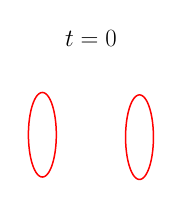
\begin{tikzpicture}[scale=0.36]

\begin{axis}[
  xmin = -6,
  xmax = 2,
  ymin = -2,
  ymax = 2,
  axis equal = true,
  hide axis,
  title = {\Huge$t=0$}
  ]

\addplot [mark=none,red,line width=1.5] table{
-4.0000e+00 1.8412e+00
-4.0563e+00 1.8329e+00
-4.1120e+00 1.8078e+00
-4.1667e+00 1.7663e+00
-4.2198e+00 1.7087e+00
-4.2707e+00 1.6356e+00
-4.3191e+00 1.5478e+00
-4.3643e+00 1.4460e+00
-4.4061e+00 1.3312e+00
-4.4439e+00 1.2046e+00
-4.4775e+00 1.0674e+00
-4.5065e+00 9.2082e-01
-4.5306e+00 7.6635e-01
-4.5496e+00 6.0546e-01
-4.5633e+00 4.3970e-01
-4.5715e+00 2.7067e-01
-4.5743e+00 1.0000e-01
-4.5715e+00 -7.0672e-02
-4.5633e+00 -2.3970e-01
-4.5496e+00 -4.0546e-01
-4.5306e+00 -5.6635e-01
-4.5065e+00 -7.2082e-01
-4.4775e+00 -8.6738e-01
-4.4439e+00 -1.0046e+00
-4.4061e+00 -1.1312e+00
-4.3643e+00 -1.2460e+00
-4.3191e+00 -1.3478e+00
-4.2707e+00 -1.4356e+00
-4.2198e+00 -1.5087e+00
-4.1667e+00 -1.5663e+00
-4.1120e+00 -1.6078e+00
-4.0563e+00 -1.6329e+00
-4.0000e+00 -1.6412e+00
-3.9437e+00 -1.6329e+00
-3.8880e+00 -1.6078e+00
-3.8333e+00 -1.5663e+00
-3.7802e+00 -1.5087e+00
-3.7293e+00 -1.4356e+00
-3.6809e+00 -1.3478e+00
-3.6357e+00 -1.2460e+00
-3.5939e+00 -1.1312e+00
-3.5561e+00 -1.0046e+00
-3.5225e+00 -8.6738e-01
-3.4935e+00 -7.2082e-01
-3.4694e+00 -5.6635e-01
-3.4504e+00 -4.0546e-01
-3.4367e+00 -2.3970e-01
-3.4285e+00 -7.0672e-02
-3.4257e+00 1.0000e-01
-3.4285e+00 2.7067e-01
-3.4367e+00 4.3970e-01
-3.4504e+00 6.0546e-01
-3.4694e+00 7.6635e-01
-3.4935e+00 9.2082e-01
-3.5225e+00 1.0674e+00
-3.5561e+00 1.2046e+00
-3.5939e+00 1.3312e+00
-3.6357e+00 1.4460e+00
-3.6809e+00 1.5478e+00
-3.7293e+00 1.6356e+00
-3.7802e+00 1.7087e+00
-3.8333e+00 1.7663e+00
-3.8880e+00 1.8078e+00
-3.9437e+00 1.8329e+00
-4.0000e+00 1.8412e+00
};

\addplot [mark=none,red,line width=1.5] table{
1.0662e-16 1.7412e+00
-5.6291e-02 1.7329e+00
-1.1204e-01 1.7078e+00
-1.6671e-01 1.6663e+00
-2.1978e-01 1.6087e+00
-2.7072e-01 1.5356e+00
-3.1907e-01 1.4478e+00
-3.6433e-01 1.3460e+00
-4.0609e-01 1.2312e+00
-4.4394e-01 1.1046e+00
-4.7751e-01 9.6738e-01
-5.0649e-01 8.2082e-01
-5.3059e-01 6.6635e-01
-5.4957e-01 5.0546e-01
-5.6327e-01 3.3970e-01
-5.7154e-01 1.7067e-01
-5.7430e-01 1.4179e-16
-5.7154e-01 -1.7067e-01
-5.6327e-01 -3.3970e-01
-5.4957e-01 -5.0546e-01
-5.3059e-01 -6.6635e-01
-5.0649e-01 -8.2082e-01
-4.7751e-01 -9.6738e-01
-4.4394e-01 -1.1046e+00
-4.0609e-01 -1.2312e+00
-3.6433e-01 -1.3460e+00
-3.1907e-01 -1.4478e+00
-2.7072e-01 -1.5356e+00
-2.1978e-01 -1.6087e+00
-1.6671e-01 -1.6663e+00
-1.1204e-01 -1.7078e+00
-5.6291e-02 -1.7329e+00
-1.7695e-16 -1.7412e+00
5.6291e-02 -1.7329e+00
1.1204e-01 -1.7078e+00
1.6671e-01 -1.6663e+00
2.1978e-01 -1.6087e+00
2.7072e-01 -1.5356e+00
3.1907e-01 -1.4478e+00
3.6433e-01 -1.3460e+00
4.0609e-01 -1.2312e+00
4.4394e-01 -1.1046e+00
4.7751e-01 -9.6738e-01
5.0649e-01 -8.2082e-01
5.3059e-01 -6.6635e-01
5.4957e-01 -5.0546e-01
5.6327e-01 -3.3970e-01
5.7154e-01 -1.7067e-01
5.7430e-01 -3.5503e-16
5.7154e-01 1.7067e-01
5.6327e-01 3.3970e-01
5.4957e-01 5.0546e-01
5.3059e-01 6.6635e-01
5.0649e-01 8.2082e-01
4.7751e-01 9.6738e-01
4.4394e-01 1.1046e+00
4.0609e-01 1.2312e+00
3.6433e-01 1.3460e+00
3.1907e-01 1.4478e+00
2.7072e-01 1.5356e+00
2.1978e-01 1.6087e+00
1.6671e-01 1.6663e+00
1.1204e-01 1.7078e+00
5.6291e-02 1.7329e+00
1.0662e-16 1.7412e+00
};

\end{axis}
\end{tikzpicture}

 &
%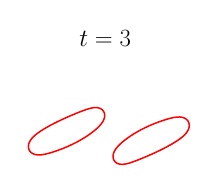
\begin{tikzpicture}[scale=0.36]

\begin{axis}[
  xmin = -6,
  xmax = 2,
  ymin = -2,
  ymax = 2,
  axis equal = true,
  hide axis,
  title = {\Huge$t=3$}
  ]

\addplot [mark=none,red,line width=1.5] table{
-2.0216e+00 8.7489e-01
-2.0233e+00 9.3267e-01
-2.0358e+00 9.9339e-01
-2.0637e+00 1.0570e+00
-2.1121e+00 1.1195e+00
-2.1842e+00 1.1728e+00
-2.2785e+00 1.2082e+00
-2.3897e+00 1.2204e+00
-2.5119e+00 1.2099e+00
-2.6416e+00 1.1811e+00
-2.7773e+00 1.1393e+00
-2.9189e+00 1.0888e+00
-3.0657e+00 1.0324e+00
-3.2171e+00 9.7161e-01
-3.3716e+00 9.0723e-01
-3.5281e+00 8.3970e-01
-3.6850e+00 7.6943e-01
-3.8409e+00 6.9686e-01
-3.9943e+00 6.2249e-01
-4.1438e+00 5.4682e-01
-4.2881e+00 4.7036e-01
-4.4256e+00 3.9354e-01
-4.5551e+00 3.1667e-01
-4.6751e+00 2.3994e-01
-4.7840e+00 1.6343e-01
-4.8804e+00 8.7178e-02
-4.9629e+00 1.1381e-02
-5.0307e+00 -6.3431e-02
-5.0831e+00 -1.3627e-01
-5.1209e+00 -2.0583e-01
-5.1454e+00 -2.7103e-01
-5.1585e+00 -3.3175e-01
-5.1622e+00 -3.8945e-01
-5.1565e+00 -4.4690e-01
-5.1396e+00 -5.0645e-01
-5.1074e+00 -5.6793e-01
-5.0556e+00 -6.2757e-01
-4.9820e+00 -6.7874e-01
-4.8877e+00 -7.1452e-01
-4.7770e+00 -7.3097e-01
-4.6543e+00 -7.2834e-01
-4.5227e+00 -7.0970e-01
-4.3840e+00 -6.7883e-01
-4.2391e+00 -6.3882e-01
-4.0890e+00 -5.9162e-01
-3.9349e+00 -5.3831e-01
-3.7781e+00 -4.7944e-01
-3.6202e+00 -4.1536e-01
-3.4628e+00 -3.4636e-01
-3.3075e+00 -2.7281e-01
-3.1557e+00 -1.9520e-01
-3.0092e+00 -1.1412e-01
-2.8691e+00 -3.0388e-02
-2.7368e+00 5.5055e-02
-2.6133e+00 1.4115e-01
-2.4997e+00 2.2684e-01
-2.3968e+00 3.1123e-01
-2.3056e+00 3.9362e-01
-2.2270e+00 4.7350e-01
-2.1618e+00 5.5041e-01
-2.1100e+00 6.2377e-01
-2.0715e+00 6.9292e-01
-2.0449e+00 7.5736e-01
-2.0288e+00 8.1744e-01
-2.0216e+00 8.7489e-01
};

\addplot [mark=none,red,line width=1.5] table{
1.4622e+00 4.8945e-01
1.4565e+00 5.4690e-01
1.4396e+00 6.0645e-01
1.4074e+00 6.6793e-01
1.3556e+00 7.2757e-01
1.2820e+00 7.7874e-01
1.1877e+00 8.1452e-01
1.0770e+00 8.3097e-01
9.5426e-01 8.2834e-01
8.2270e-01 8.0970e-01
6.8398e-01 7.7883e-01
5.3908e-01 7.3882e-01
3.8899e-01 6.9162e-01
2.3487e-01 6.3831e-01
7.8119e-02 5.7944e-01
-7.9760e-02 5.1536e-01
-2.3718e-01 4.4636e-01
-3.9253e-01 3.7281e-01
-5.4425e-01 2.9520e-01
-6.9083e-01 2.1412e-01
-8.3089e-01 1.3039e-01
-9.6319e-01 4.4945e-02
-1.0867e+00 -4.1147e-02
-1.2003e+00 -1.2684e-01
-1.3032e+00 -2.1123e-01
-1.3944e+00 -2.9362e-01
-1.4730e+00 -3.7350e-01
-1.5382e+00 -4.5041e-01
-1.5900e+00 -5.2377e-01
-1.6285e+00 -5.9292e-01
-1.6551e+00 -6.5736e-01
-1.6712e+00 -7.1744e-01
-1.6784e+00 -7.7489e-01
-1.6767e+00 -8.3267e-01
-1.6642e+00 -8.9339e-01
-1.6363e+00 -9.5703e-01
-1.5879e+00 -1.0195e+00
-1.5158e+00 -1.0728e+00
-1.4215e+00 -1.1082e+00
-1.3103e+00 -1.1204e+00
-1.1881e+00 -1.1099e+00
-1.0584e+00 -1.0811e+00
-9.2265e-01 -1.0393e+00
-7.8111e-01 -9.8879e-01
-6.3425e-01 -9.3239e-01
-4.8294e-01 -8.7161e-01
-3.2837e-01 -8.0723e-01
-1.7190e-01 -7.3970e-01
-1.5005e-02 -6.6943e-01
1.4087e-01 -5.9686e-01
2.9428e-01 -5.2249e-01
4.4381e-01 -4.4682e-01
5.8806e-01 -3.7036e-01
7.2564e-01 -2.9354e-01
8.5513e-01 -2.1667e-01
9.7508e-01 -1.3994e-01
1.0840e+00 -6.3428e-02
1.1804e+00 1.2822e-02
1.2629e+00 8.8619e-02
1.3307e+00 1.6343e-01
1.3831e+00 2.3627e-01
1.4209e+00 3.0583e-01
1.4454e+00 3.7103e-01
1.4585e+00 4.3175e-01
1.4622e+00 4.8945e-01
};

\end{axis}
\end{tikzpicture}

 &
%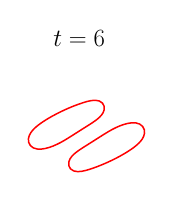
\begin{tikzpicture}[scale=0.36]

\begin{axis}[
  xmin = -6,
  xmax = 2,
  ymin = -2,
  ymax = 2,
  axis equal = true,
  hide axis,
  title = {\Huge$t=6$}
  ]

\addplot [mark=none,red,line width=1.5] table{
-1.5410e+00 5.4046e-01
-1.4923e+00 5.7219e-01
-1.4402e+00 6.0678e-01
-1.3823e+00 6.4647e-01
-1.3172e+00 6.9321e-01
-1.2451e+00 7.4900e-01
-1.1676e+00 8.1643e-01
-1.0891e+00 8.9908e-01
-1.0179e+00 1.0017e+00
-9.7044e-01 1.1277e+00
-9.7153e-01 1.2707e+00
-1.0418e+00 1.4034e+00
-1.1725e+00 1.4898e+00
-1.3324e+00 1.5193e+00
-1.4993e+00 1.5070e+00
-1.6658e+00 1.4711e+00
-1.8309e+00 1.4230e+00
-1.9938e+00 1.3681e+00
-2.1538e+00 1.3092e+00
-2.3097e+00 1.2476e+00
-2.4601e+00 1.1842e+00
-2.6040e+00 1.1199e+00
-2.7403e+00 1.0558e+00
-2.8679e+00 9.9261e-01
-2.9861e+00 9.3139e-01
-3.0943e+00 8.7295e-01
-3.1920e+00 8.1798e-01
-3.2793e+00 7.6701e-01
-3.3561e+00 7.2039e-01
-3.4233e+00 6.7817e-01
-3.4818e+00 6.4007e-01
-3.5336e+00 6.0522e-01
-3.5813e+00 5.7199e-01
-3.6284e+00 5.3794e-01
-3.6782e+00 5.0032e-01
-3.7331e+00 4.5661e-01
-3.7939e+00 4.0460e-01
-3.8601e+00 3.4210e-01
-3.9295e+00 2.6669e-01
-3.9975e+00 1.7547e-01
-4.0558e+00 6.5359e-02
-4.0903e+00 -6.4585e-02
-4.0815e+00 -2.0741e-01
-4.0137e+00 -3.4173e-01
-3.8907e+00 -4.3937e-01
-3.7351e+00 -4.8701e-01
-3.5680e+00 -4.9161e-01
-3.3995e+00 -4.6660e-01
-3.2335e+00 -4.2208e-01
-3.0718e+00 -3.6385e-01
-2.9158e+00 -2.9542e-01
-2.7663e+00 -2.1982e-01
-2.6239e+00 -1.4009e-01
-2.4888e+00 -5.9196e-02
-2.3610e+00 2.0337e-02
-2.2407e+00 9.6581e-02
-2.1285e+00 1.6817e-01
-2.0249e+00 2.3421e-01
-1.9302e+00 2.9425e-01
-1.8449e+00 3.4813e-01
-1.7688e+00 3.9601e-01
-1.7017e+00 4.3826e-01
-1.6426e+00 4.7556e-01
-1.5899e+00 5.0904e-01
-1.5410e+00 5.4046e-01
};

\addplot [mark=none,red,line width=1.5] table{
1.8128e-01 -4.7199e-01
2.2837e-01 -4.3794e-01
2.7821e-01 -4.0032e-01
3.3307e-01 -3.5661e-01
3.9388e-01 -3.0460e-01
4.6009e-01 -2.4210e-01
5.2951e-01 -1.6669e-01
5.9754e-01 -7.5465e-02
6.5584e-01 3.4641e-02
6.9030e-01 1.6458e-01
6.8152e-01 3.0741e-01
6.1369e-01 4.4173e-01
4.9073e-01 5.3937e-01
3.3515e-01 5.8701e-01
1.6796e-01 5.9161e-01
-4.8922e-04 5.6660e-01
-1.6646e-01 5.2208e-01
-3.2815e-01 4.6385e-01
-4.8423e-01 3.9542e-01
-6.3370e-01 3.1982e-01
-7.7608e-01 2.4009e-01
-9.1123e-01 1.5920e-01
-1.0390e+00 7.9663e-02
-1.1593e+00 3.4189e-03
-1.2715e+00 -6.8167e-02
-1.3751e+00 -1.3421e-01
-1.4698e+00 -1.9425e-01
-1.5551e+00 -2.4813e-01
-1.6312e+00 -2.9601e-01
-1.6983e+00 -3.3826e-01
-1.7574e+00 -3.7556e-01
-1.8101e+00 -4.0904e-01
-1.8590e+00 -4.4046e-01
-1.9077e+00 -4.7219e-01
-1.9598e+00 -5.0678e-01
-2.0177e+00 -5.4647e-01
-2.0828e+00 -5.9321e-01
-2.1549e+00 -6.4900e-01
-2.2324e+00 -7.1643e-01
-2.3109e+00 -7.9908e-01
-2.3821e+00 -9.0168e-01
-2.4296e+00 -1.0277e+00
-2.4285e+00 -1.1707e+00
-2.3582e+00 -1.3034e+00
-2.2275e+00 -1.3898e+00
-2.0676e+00 -1.4193e+00
-1.9007e+00 -1.4070e+00
-1.7342e+00 -1.3711e+00
-1.5691e+00 -1.3230e+00
-1.4062e+00 -1.2681e+00
-1.2462e+00 -1.2092e+00
-1.0903e+00 -1.1476e+00
-9.3986e-01 -1.0842e+00
-7.9598e-01 -1.0199e+00
-6.5973e-01 -9.5576e-01
-5.3209e-01 -8.9261e-01
-4.1387e-01 -8.3139e-01
-3.0569e-01 -7.7295e-01
-2.0795e-01 -7.1798e-01
-1.2075e-01 -6.6701e-01
-4.3859e-02 -6.2039e-01
2.3301e-02 -5.7817e-01
8.1850e-02 -5.4007e-01
1.3359e-01 -5.0522e-01
1.8128e-01 -4.7199e-01
};

\end{axis}
\end{tikzpicture}

 &
%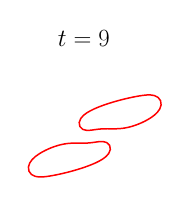
\begin{tikzpicture}[scale=0.36]

\begin{axis}[
  xmin = -6,
  xmax = 2,
  ymin = -2,
  ymax = 2,
  axis equal = true,
  hide axis,
  title = {\Huge$t=9$}
  ]

\addplot [mark=none,red,line width=1.5] table{
-4.3957e-01 3.6041e-01
-3.8178e-01 3.6751e-01
-3.1988e-01 3.7671e-01
-2.5066e-01 3.8903e-01
-1.7215e-01 4.0552e-01
-8.3497e-02 4.2740e-01
1.5384e-02 4.5571e-01
1.2394e-01 4.9146e-01
2.4132e-01 5.3538e-01
3.6627e-01 5.8815e-01
4.9734e-01 6.5032e-01
6.3253e-01 7.2278e-01
7.6930e-01 8.0693e-01
9.0353e-01 9.0552e-01
1.0280e+00 1.0229e+00
1.1288e+00 1.1646e+00
1.1818e+00 1.3307e+00
1.1588e+00 1.5019e+00
1.0562e+00 1.6376e+00
9.0703e-01 1.7131e+00
7.4599e-01 1.7389e+00
5.8841e-01 1.7366e+00
4.3855e-01 1.7211e+00
2.9763e-01 1.7002e+00
1.6642e-01 1.6772e+00
4.5633e-02 1.6539e+00
-6.4224e-02 1.6311e+00
-1.6293e-01 1.6094e+00
-2.5060e-01 1.5892e+00
-3.2778e-01 1.5707e+00
-3.9562e-01 1.5539e+00
-4.5611e-01 1.5385e+00
-5.1237e-01 1.5238e+00
-5.6854e-01 1.5087e+00
-6.2880e-01 1.4922e+00
-6.9637e-01 1.4731e+00
-7.7328e-01 1.4508e+00
-8.6058e-01 1.4246e+00
-9.5856e-01 1.3941e+00
-1.0670e+00 1.3587e+00
-1.1852e+00 1.3181e+00
-1.3122e+00 1.2715e+00
-1.4469e+00 1.2183e+00
-1.5873e+00 1.1572e+00
-1.7314e+00 1.0864e+00
-1.8751e+00 1.0023e+00
-2.0118e+00 8.9956e-01
-2.1269e+00 7.6930e-01
-2.1908e+00 6.0729e-01
-2.1627e+00 4.3764e-01
-2.0411e+00 3.1999e-01
-1.8791e+00 2.7936e-01
-1.7161e+00 2.8575e-01
-1.5599e+00 3.0741e-01
-1.4106e+00 3.2740e-01
-1.2687e+00 3.4022e-01
-1.1355e+00 3.4571e-01
-1.0125e+00 3.4645e-01
-9.0021e-01 3.4522e-01
-7.9912e-01 3.4426e-01
-7.0911e-01 3.4463e-01
-6.2971e-01 3.4665e-01
-5.5984e-01 3.5010e-01
-4.9752e-01 3.5472e-01
-4.3957e-01 3.6041e-01
};

\addplot [mark=none,red,line width=1.5] table{
-2.5876e+00 -1.4238e+00
-2.5315e+00 -1.4087e+00
-2.4712e+00 -1.3922e+00
-2.4036e+00 -1.3731e+00
-2.3267e+00 -1.3508e+00
-2.2394e+00 -1.3246e+00
-2.1414e+00 -1.2941e+00
-2.0330e+00 -1.2587e+00
-1.9148e+00 -1.2181e+00
-1.7878e+00 -1.1715e+00
-1.6531e+00 -1.1183e+00
-1.5127e+00 -1.0572e+00
-1.3686e+00 -9.8637e-01
-1.2249e+00 -9.0234e-01
-1.0882e+00 -7.9956e-01
-9.7311e-01 -6.6930e-01
-9.0918e-01 -5.0729e-01
-9.3734e-01 -3.3764e-01
-1.0589e+00 -2.1999e-01
-1.2209e+00 -1.7936e-01
-1.3839e+00 -1.8575e-01
-1.5401e+00 -2.0741e-01
-1.6894e+00 -2.2740e-01
-1.8313e+00 -2.4022e-01
-1.9645e+00 -2.4571e-01
-2.0875e+00 -2.4645e-01
-2.1998e+00 -2.4522e-01
-2.3009e+00 -2.4426e-01
-2.3909e+00 -2.4463e-01
-2.4703e+00 -2.4665e-01
-2.5402e+00 -2.5010e-01
-2.6025e+00 -2.5472e-01
-2.6604e+00 -2.6041e-01
-2.7182e+00 -2.6751e-01
-2.7801e+00 -2.7671e-01
-2.8493e+00 -2.8903e-01
-2.9279e+00 -3.0552e-01
-3.0165e+00 -3.2740e-01
-3.1154e+00 -3.5571e-01
-3.2239e+00 -3.9146e-01
-3.3413e+00 -4.3538e-01
-3.4663e+00 -4.8815e-01
-3.5973e+00 -5.5032e-01
-3.7325e+00 -6.2278e-01
-3.8693e+00 -7.0693e-01
-4.0035e+00 -8.0552e-01
-4.1280e+00 -9.2295e-01
-4.2288e+00 -1.0646e+00
-4.2818e+00 -1.2307e+00
-4.2588e+00 -1.4019e+00
-4.1562e+00 -1.5376e+00
-4.0070e+00 -1.6131e+00
-3.8460e+00 -1.6389e+00
-3.6884e+00 -1.6366e+00
-3.5386e+00 -1.6211e+00
-3.3976e+00 -1.6002e+00
-3.2664e+00 -1.5772e+00
-3.1456e+00 -1.5539e+00
-3.0358e+00 -1.5311e+00
-2.9371e+00 -1.5094e+00
-2.8494e+00 -1.4892e+00
-2.7722e+00 -1.4707e+00
-2.7044e+00 -1.4539e+00
-2.6439e+00 -1.4385e+00
-2.5876e+00 -1.4238e+00
};

\end{axis}
\end{tikzpicture}

 &
%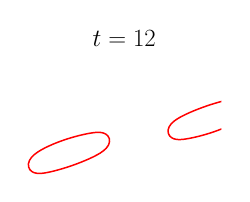
\begin{tikzpicture}[scale=0.36]

\begin{axis}[
  xmin = -6,
  xmax = 2,
  ymin = -2,
  ymax = 2,
  axis equal = true,
  hide axis,
  title = {\Huge$t=12$}
  ]

\addplot [mark=none,red,line width=1.5] table{
4.0724e-01 -9.1055e-02
4.6516e-01 -8.4515e-02
5.2711e-01 -7.5991e-02
5.9659e-01 -6.4890e-02
6.7552e-01 -5.0781e-02
7.6518e-01 -3.3150e-02
8.6573e-01 -1.1733e-02
9.7719e-01 1.3863e-02
1.0988e+00 4.3860e-02
1.2300e+00 7.8635e-02
1.3695e+00 1.1836e-01
1.5162e+00 1.6330e-01
1.6688e+00 2.1349e-01
1.8260e+00 2.6903e-01
1.9862e+00 3.2984e-01
2.1479e+00 3.9590e-01
2.3089e+00 4.6710e-01
2.4676e+00 5.4375e-01
2.6213e+00 6.2646e-01
2.7672e+00 7.1672e-01
2.9008e+00 8.1675e-01
3.0157e+00 9.2954e-01
3.1013e+00 1.0567e+00
3.1451e+00 1.1943e+00
3.1376e+00 1.3284e+00
3.0837e+00 1.4395e+00
3.0016e+00 1.5162e+00
2.9111e+00 1.5613e+00
2.8238e+00 1.5837e+00
2.7449e+00 1.5924e+00
2.6750e+00 1.5934e+00
2.6127e+00 1.5903e+00
2.5547e+00 1.5847e+00
2.4971e+00 1.5772e+00
2.4353e+00 1.5674e+00
2.3663e+00 1.5547e+00
2.2878e+00 1.5386e+00
2.1989e+00 1.5187e+00
2.0991e+00 1.4946e+00
1.9888e+00 1.4661e+00
1.8682e+00 1.4330e+00
1.7383e+00 1.3952e+00
1.5999e+00 1.3525e+00
1.4543e+00 1.3050e+00
1.3025e+00 1.2525e+00
1.1460e+00 1.1955e+00
9.8599e-01 1.1339e+00
8.2420e-01 1.0681e+00
6.6208e-01 9.9817e-01
5.0178e-01 9.2403e-01
3.4527e-01 8.4480e-01
1.9568e-01 7.5876e-01
5.7673e-02 6.6303e-01
-6.1168e-02 5.5398e-01
-1.5005e-01 4.2875e-01
-1.9434e-01 2.9128e-01
-1.8435e-01 1.5733e-01
-1.2647e-01 4.8230e-02
-4.1697e-02 -2.5554e-02
5.0197e-02 -6.7980e-02
1.3773e-01 -8.8984e-02
2.1681e-01 -9.7173e-02
2.8673e-01 -9.8374e-02
3.4924e-01 -9.5786e-02
4.0724e-01 -9.1055e-02
};

\addplot [mark=none,red,line width=1.5] table{
-5.3547e+00 -1.4847e+00
-5.2971e+00 -1.4772e+00
-5.2353e+00 -1.4674e+00
-5.1663e+00 -1.4547e+00
-5.0878e+00 -1.4386e+00
-4.9989e+00 -1.4187e+00
-4.8991e+00 -1.3946e+00
-4.7888e+00 -1.3661e+00
-4.6682e+00 -1.3330e+00
-4.5383e+00 -1.2952e+00
-4.3999e+00 -1.2525e+00
-4.2543e+00 -1.2050e+00
-4.1025e+00 -1.1525e+00
-3.9460e+00 -1.0955e+00
-3.7860e+00 -1.0339e+00
-3.6242e+00 -9.6810e-01
-3.4621e+00 -8.9817e-01
-3.3018e+00 -8.2403e-01
-3.1453e+00 -7.4480e-01
-2.9957e+00 -6.5876e-01
-2.8577e+00 -5.6303e-01
-2.7388e+00 -4.5398e-01
-2.6499e+00 -3.2875e-01
-2.6057e+00 -1.9128e-01
-2.6156e+00 -5.7335e-02
-2.6735e+00 5.1770e-02
-2.7583e+00 1.2555e-01
-2.8502e+00 1.6798e-01
-2.9377e+00 1.8898e-01
-3.0168e+00 1.9717e-01
-3.0867e+00 1.9837e-01
-3.1492e+00 1.9579e-01
-3.2072e+00 1.9105e-01
-3.2652e+00 1.8451e-01
-3.3271e+00 1.7599e-01
-3.3966e+00 1.6489e-01
-3.4755e+00 1.5078e-01
-3.5652e+00 1.3315e-01
-3.6657e+00 1.1173e-01
-3.7772e+00 8.6137e-02
-3.8988e+00 5.6140e-02
-4.0300e+00 2.1365e-02
-4.1695e+00 -1.8363e-02
-4.3162e+00 -6.3304e-02
-4.4688e+00 -1.1349e-01
-4.6260e+00 -1.6903e-01
-4.7862e+00 -2.2984e-01
-4.9479e+00 -2.9590e-01
-5.1089e+00 -3.6710e-01
-5.2676e+00 -4.4375e-01
-5.4213e+00 -5.2646e-01
-5.5672e+00 -6.1672e-01
-5.7008e+00 -7.1675e-01
-5.8157e+00 -8.2954e-01
-5.9013e+00 -9.5669e-01
-5.9451e+00 -1.0943e+00
-5.9376e+00 -1.2284e+00
-5.8837e+00 -1.3395e+00
-5.8016e+00 -1.4162e+00
-5.7111e+00 -1.4613e+00
-5.6238e+00 -1.4837e+00
-5.5449e+00 -1.4924e+00
-5.4750e+00 -1.4934e+00
-5.4127e+00 -1.4903e+00
-5.3547e+00 -1.4847e+00
};

\end{axis}
\end{tikzpicture}


%\fi
%\end{tabular}
%\begin{tabular}{m{1cm}CCCCC}
%\ifInputs
%$\nu=4$ &
%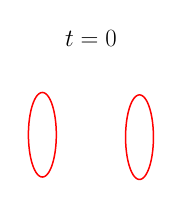
\begin{tikzpicture}[scale=0.36]

\begin{axis}[
  xmin = -6,
  xmax = 2,
  ymin = -2,
  ymax = 2,
  axis equal = true,
  hide axis,
  title = {\Huge$t=0$}
  ]

\addplot [mark=none,red,line width=1.5] table{
-4.0000e+00 1.8412e+00
-4.0563e+00 1.8329e+00
-4.1120e+00 1.8078e+00
-4.1667e+00 1.7663e+00
-4.2198e+00 1.7087e+00
-4.2707e+00 1.6356e+00
-4.3191e+00 1.5478e+00
-4.3643e+00 1.4460e+00
-4.4061e+00 1.3312e+00
-4.4439e+00 1.2046e+00
-4.4775e+00 1.0674e+00
-4.5065e+00 9.2082e-01
-4.5306e+00 7.6635e-01
-4.5496e+00 6.0546e-01
-4.5633e+00 4.3970e-01
-4.5715e+00 2.7067e-01
-4.5743e+00 1.0000e-01
-4.5715e+00 -7.0672e-02
-4.5633e+00 -2.3970e-01
-4.5496e+00 -4.0546e-01
-4.5306e+00 -5.6635e-01
-4.5065e+00 -7.2082e-01
-4.4775e+00 -8.6738e-01
-4.4439e+00 -1.0046e+00
-4.4061e+00 -1.1312e+00
-4.3643e+00 -1.2460e+00
-4.3191e+00 -1.3478e+00
-4.2707e+00 -1.4356e+00
-4.2198e+00 -1.5087e+00
-4.1667e+00 -1.5663e+00
-4.1120e+00 -1.6078e+00
-4.0563e+00 -1.6329e+00
-4.0000e+00 -1.6412e+00
-3.9437e+00 -1.6329e+00
-3.8880e+00 -1.6078e+00
-3.8333e+00 -1.5663e+00
-3.7802e+00 -1.5087e+00
-3.7293e+00 -1.4356e+00
-3.6809e+00 -1.3478e+00
-3.6357e+00 -1.2460e+00
-3.5939e+00 -1.1312e+00
-3.5561e+00 -1.0046e+00
-3.5225e+00 -8.6738e-01
-3.4935e+00 -7.2082e-01
-3.4694e+00 -5.6635e-01
-3.4504e+00 -4.0546e-01
-3.4367e+00 -2.3970e-01
-3.4285e+00 -7.0672e-02
-3.4257e+00 1.0000e-01
-3.4285e+00 2.7067e-01
-3.4367e+00 4.3970e-01
-3.4504e+00 6.0546e-01
-3.4694e+00 7.6635e-01
-3.4935e+00 9.2082e-01
-3.5225e+00 1.0674e+00
-3.5561e+00 1.2046e+00
-3.5939e+00 1.3312e+00
-3.6357e+00 1.4460e+00
-3.6809e+00 1.5478e+00
-3.7293e+00 1.6356e+00
-3.7802e+00 1.7087e+00
-3.8333e+00 1.7663e+00
-3.8880e+00 1.8078e+00
-3.9437e+00 1.8329e+00
-4.0000e+00 1.8412e+00
};

\addplot [mark=none,red,line width=1.5] table{
1.0662e-16 1.7412e+00
-5.6291e-02 1.7329e+00
-1.1204e-01 1.7078e+00
-1.6671e-01 1.6663e+00
-2.1978e-01 1.6087e+00
-2.7072e-01 1.5356e+00
-3.1907e-01 1.4478e+00
-3.6433e-01 1.3460e+00
-4.0609e-01 1.2312e+00
-4.4394e-01 1.1046e+00
-4.7751e-01 9.6738e-01
-5.0649e-01 8.2082e-01
-5.3059e-01 6.6635e-01
-5.4957e-01 5.0546e-01
-5.6327e-01 3.3970e-01
-5.7154e-01 1.7067e-01
-5.7430e-01 1.4179e-16
-5.7154e-01 -1.7067e-01
-5.6327e-01 -3.3970e-01
-5.4957e-01 -5.0546e-01
-5.3059e-01 -6.6635e-01
-5.0649e-01 -8.2082e-01
-4.7751e-01 -9.6738e-01
-4.4394e-01 -1.1046e+00
-4.0609e-01 -1.2312e+00
-3.6433e-01 -1.3460e+00
-3.1907e-01 -1.4478e+00
-2.7072e-01 -1.5356e+00
-2.1978e-01 -1.6087e+00
-1.6671e-01 -1.6663e+00
-1.1204e-01 -1.7078e+00
-5.6291e-02 -1.7329e+00
-1.7695e-16 -1.7412e+00
5.6291e-02 -1.7329e+00
1.1204e-01 -1.7078e+00
1.6671e-01 -1.6663e+00
2.1978e-01 -1.6087e+00
2.7072e-01 -1.5356e+00
3.1907e-01 -1.4478e+00
3.6433e-01 -1.3460e+00
4.0609e-01 -1.2312e+00
4.4394e-01 -1.1046e+00
4.7751e-01 -9.6738e-01
5.0649e-01 -8.2082e-01
5.3059e-01 -6.6635e-01
5.4957e-01 -5.0546e-01
5.6327e-01 -3.3970e-01
5.7154e-01 -1.7067e-01
5.7430e-01 -3.5503e-16
5.7154e-01 1.7067e-01
5.6327e-01 3.3970e-01
5.4957e-01 5.0546e-01
5.3059e-01 6.6635e-01
5.0649e-01 8.2082e-01
4.7751e-01 9.6738e-01
4.4394e-01 1.1046e+00
4.0609e-01 1.2312e+00
3.6433e-01 1.3460e+00
3.1907e-01 1.4478e+00
2.7072e-01 1.5356e+00
2.1978e-01 1.6087e+00
1.6671e-01 1.6663e+00
1.1204e-01 1.7078e+00
5.6291e-02 1.7329e+00
1.0662e-16 1.7412e+00
};

\end{axis}
\end{tikzpicture}

 &
%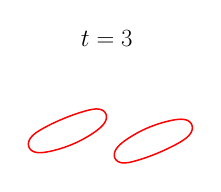
\begin{tikzpicture}[scale=0.36]

\begin{axis}[
  xmin = -6,
  xmax = 2,
  ymin = -2,
  ymax = 2,
  axis equal = true,
  hide axis,
  title = {\Huge$t=3$}
  ]

\addplot [mark=none,red,line width=1.5] table{
-2.0156e+00 8.9140e-01
-2.0309e+00 9.4675e-01
-2.0587e+00 1.0019e+00
-2.1023e+00 1.0555e+00
-2.1649e+00 1.1033e+00
-2.2469e+00 1.1394e+00
-2.3457e+00 1.1590e+00
-2.4576e+00 1.1610e+00
-2.5796e+00 1.1473e+00
-2.7099e+00 1.1215e+00
-2.8477e+00 1.0869e+00
-2.9922e+00 1.0456e+00
-3.1425e+00 9.9896e-01
-3.2972e+00 9.4748e-01
-3.4550e+00 8.9145e-01
-3.6143e+00 8.3116e-01
-3.7737e+00 7.6703e-01
-3.9318e+00 6.9967e-01
-4.0873e+00 6.2985e-01
-4.2388e+00 5.5845e-01
-4.3851e+00 4.8630e-01
-4.5250e+00 4.1402e-01
-4.6571e+00 3.4186e-01
-4.7797e+00 2.6955e-01
-4.8910e+00 1.9646e-01
-4.9887e+00 1.2185e-01
-5.0707e+00 4.5480e-02
-5.1353e+00 -3.1905e-02
-5.1816e+00 -1.0844e-01
-5.2104e+00 -1.8159e-01
-5.2239e+00 -2.4925e-01
-5.2250e+00 -3.1077e-01
-5.2159e+00 -3.6742e-01
-5.1969e+00 -4.2158e-01
-5.1659e+00 -4.7488e-01
-5.1198e+00 -5.2646e-01
-5.0561e+00 -5.7276e-01
-4.9741e+00 -6.0902e-01
-4.8759e+00 -6.3153e-01
-4.7641e+00 -6.3921e-01
-4.6415e+00 -6.3339e-01
-4.5096e+00 -6.1654e-01
-4.3698e+00 -5.9100e-01
-4.2231e+00 -5.5833e-01
-4.0706e+00 -5.1929e-01
-3.9139e+00 -4.7410e-01
-3.7545e+00 -4.2279e-01
-3.5941e+00 -3.6541e-01
-3.4344e+00 -3.0219e-01
-3.2768e+00 -2.3357e-01
-3.1231e+00 -1.6024e-01
-2.9745e+00 -8.3146e-02
-2.8322e+00 -3.4254e-03
-2.6973e+00 7.7735e-02
-2.5709e+00 1.5927e-01
-2.4540e+00 2.4044e-01
-2.3481e+00 3.2093e-01
-2.2545e+00 4.0074e-01
-2.1751e+00 4.7988e-01
-2.1114e+00 5.5795e-01
-2.0640e+00 6.3385e-01
-2.0326e+00 7.0596e-01
-2.0155e+00 7.7286e-01
-2.0105e+00 8.3423e-01
-2.0156e+00 8.9140e-01
};

\addplot [mark=none,red,line width=1.5] table{
1.5159e+00 4.6742e-01
1.4969e+00 5.2158e-01
1.4659e+00 5.7488e-01
1.4198e+00 6.2646e-01
1.3561e+00 6.7276e-01
1.2741e+00 7.0902e-01
1.1759e+00 7.3153e-01
1.0641e+00 7.3921e-01
9.4149e-01 7.3339e-01
8.0965e-01 7.1654e-01
6.6981e-01 6.9100e-01
5.2305e-01 6.5833e-01
3.7062e-01 6.1929e-01
2.1393e-01 5.7410e-01
5.4550e-02 5.2279e-01
-1.0586e-01 4.6541e-01
-2.6564e-01 4.0219e-01
-4.2317e-01 3.3357e-01
-5.7692e-01 2.6024e-01
-7.2554e-01 1.8315e-01
-8.6781e-01 1.0343e-01
-1.0027e+00 2.2265e-02
-1.1291e+00 -5.9272e-02
-1.2460e+00 -1.4044e-01
-1.3519e+00 -2.2093e-01
-1.4455e+00 -3.0074e-01
-1.5249e+00 -3.7988e-01
-1.5886e+00 -4.5795e-01
-1.6360e+00 -5.3385e-01
-1.6674e+00 -6.0596e-01
-1.6845e+00 -6.7286e-01
-1.6895e+00 -7.3423e-01
-1.6844e+00 -7.9140e-01
-1.6691e+00 -8.4675e-01
-1.6413e+00 -9.0185e-01
-1.5977e+00 -9.5551e-01
-1.5351e+00 -1.0033e+00
-1.4531e+00 -1.0394e+00
-1.3543e+00 -1.0590e+00
-1.2424e+00 -1.0610e+00
-1.1204e+00 -1.0473e+00
-9.9009e-01 -1.0215e+00
-8.5228e-01 -9.8688e-01
-7.0775e-01 -9.4561e-01
-5.5751e-01 -8.9896e-01
-4.0280e-01 -8.4748e-01
-2.4503e-01 -7.9145e-01
-8.5698e-02 -7.3116e-01
7.3733e-02 -6.6703e-01
2.3184e-01 -5.9967e-01
3.8727e-01 -5.2985e-01
5.3877e-01 -4.5845e-01
6.8509e-01 -3.8630e-01
8.2500e-01 -3.1402e-01
9.5707e-01 -2.4186e-01
1.0797e+00 -1.6955e-01
1.1910e+00 -9.6456e-02
1.2887e+00 -2.1847e-02
1.3707e+00 5.4520e-02
1.4353e+00 1.3191e-01
1.4816e+00 2.0844e-01
1.5104e+00 2.8159e-01
1.5239e+00 3.4925e-01
1.5250e+00 4.1077e-01
1.5159e+00 4.6742e-01
};

\end{axis}
\end{tikzpicture}

 &
%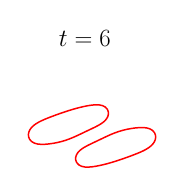
\begin{tikzpicture}[scale=0.36]

\begin{axis}[
  xmin = -6,
  xmax = 2,
  ymin = -2,
  ymax = 2,
  axis equal = true,
  hide axis,
  title = {\Huge$t=6$}
  ]

\addplot [mark=none,red,line width=1.5] table{
-1.2106e+00 6.3920e-01
-1.1683e+00 6.7850e-01
-1.1266e+00 7.2449e-01
-1.0860e+00 7.8110e-01
-1.0501e+00 8.5192e-01
-1.0270e+00 9.3903e-01
-1.0288e+00 1.0401e+00
-1.0680e+00 1.1450e+00
-1.1497e+00 1.2363e+00
-1.2667e+00 1.2987e+00
-1.4053e+00 1.3287e+00
-1.5555e+00 1.3328e+00
-1.7122e+00 1.3194e+00
-1.8734e+00 1.2947e+00
-2.0376e+00 1.2621e+00
-2.2036e+00 1.2236e+00
-2.3698e+00 1.1800e+00
-2.5350e+00 1.1324e+00
-2.6977e+00 1.0818e+00
-2.8568e+00 1.0294e+00
-3.0111e+00 9.7626e-01
-3.1594e+00 9.2348e-01
-3.3008e+00 8.7172e-01
-3.4340e+00 8.2137e-01
-3.5578e+00 7.7252e-01
-3.6714e+00 7.2509e-01
-3.7736e+00 6.7896e-01
-3.8641e+00 6.3414e-01
-3.9425e+00 5.9079e-01
-4.0094e+00 5.4914e-01
-4.0660e+00 5.0927e-01
-4.1142e+00 4.7065e-01
-4.1567e+00 4.3173e-01
-4.1962e+00 3.8969e-01
-4.2345e+00 3.4087e-01
-4.2709e+00 2.8148e-01
-4.3016e+00 2.0834e-01
-4.3193e+00 1.1999e-01
-4.3130e+00 1.9028e-02
-4.2719e+00 -8.5227e-02
-4.1913e+00 -1.7765e-01
-4.0769e+00 -2.4481e-01
-3.9401e+00 -2.8278e-01
-3.7904e+00 -2.9635e-01
-3.6331e+00 -2.9292e-01
-3.4707e+00 -2.7809e-01
-3.3049e+00 -2.5460e-01
-3.1375e+00 -2.2309e-01
-2.9704e+00 -1.8317e-01
-2.8056e+00 -1.3457e-01
-2.6449e+00 -7.7957e-02
-2.4896e+00 -1.5256e-02
-2.3405e+00 5.0800e-02
-2.1979e+00 1.1739e-01
-2.0621e+00 1.8219e-01
-1.9337e+00 2.4362e-01
-1.8135e+00 3.0085e-01
-1.7025e+00 3.5373e-01
-1.6015e+00 4.0256e-01
-1.5113e+00 4.4784e-01
-1.4322e+00 4.9007e-01
-1.3641e+00 5.2964e-01
-1.3058e+00 5.6700e-01
-1.2555e+00 6.0296e-01
-1.2106e+00 6.3920e-01
};

\addplot [mark=none,red,line width=1.5] table{
7.5671e-01 -3.3173e-01
7.9624e-01 -2.8969e-01
8.3450e-01 -2.4087e-01
8.7088e-01 -1.8148e-01
9.0163e-01 -1.0834e-01
9.1926e-01 -1.9988e-02
9.1298e-01 8.0972e-02
8.7189e-01 1.8523e-01
7.9133e-01 2.7765e-01
6.7693e-01 3.4481e-01
5.4011e-01 3.8278e-01
3.9045e-01 3.9635e-01
2.3314e-01 3.9292e-01
7.0732e-02 3.7809e-01
-9.5056e-02 3.5460e-01
-2.6249e-01 3.2309e-01
-4.2963e-01 2.8317e-01
-5.9444e-01 2.3457e-01
-7.5512e-01 1.7796e-01
-9.1036e-01 1.1526e-01
-1.0595e+00 4.9200e-02
-1.2021e+00 -1.7392e-02
-1.3379e+00 -8.2192e-02
-1.4663e+00 -1.4362e-01
-1.5865e+00 -2.0085e-01
-1.6975e+00 -2.5373e-01
-1.7985e+00 -3.0256e-01
-1.8887e+00 -3.4784e-01
-1.9678e+00 -3.9007e-01
-2.0359e+00 -4.2964e-01
-2.0942e+00 -4.6700e-01
-2.1445e+00 -5.0296e-01
-2.1894e+00 -5.3920e-01
-2.2317e+00 -5.7850e-01
-2.2734e+00 -6.2449e-01
-2.3140e+00 -6.8110e-01
-2.3499e+00 -7.5192e-01
-2.3730e+00 -8.3903e-01
-2.3712e+00 -9.4015e-01
-2.3320e+00 -1.0450e+00
-2.2503e+00 -1.1363e+00
-2.1333e+00 -1.1987e+00
-1.9947e+00 -1.2287e+00
-1.8445e+00 -1.2328e+00
-1.6878e+00 -1.2194e+00
-1.5266e+00 -1.1947e+00
-1.3624e+00 -1.1621e+00
-1.1964e+00 -1.1236e+00
-1.0302e+00 -1.0800e+00
-8.6504e-01 -1.0324e+00
-7.0232e-01 -9.8177e-01
-5.4324e-01 -9.2935e-01
-3.8895e-01 -8.7626e-01
-2.4057e-01 -8.2348e-01
-9.9226e-02 -7.7172e-01
3.3956e-02 -7.2137e-01
1.5784e-01 -6.7252e-01
2.7137e-01 -6.2509e-01
3.7364e-01 -5.7896e-01
4.6405e-01 -5.3414e-01
5.4248e-01 -4.9079e-01
6.0940e-01 -4.4914e-01
6.6599e-01 -4.0927e-01
7.1421e-01 -3.7065e-01
7.5671e-01 -3.3173e-01
};

\end{axis}
\end{tikzpicture}

 &
%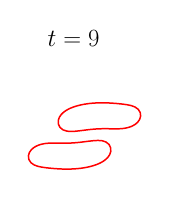
\begin{tikzpicture}[scale=0.36]

\begin{axis}[
  xmin = -6,
  xmax = 2,
  ymin = -2,
  ymax = 2,
  axis equal = true,
  hide axis,
  title = {\Huge$t=9$}
  ]

\addplot [mark=none,red,line width=1.5] table{
1.1293e-02 3.5515e-01
6.8710e-02 3.6215e-01
1.3014e-01 3.7188e-01
1.9860e-01 3.8587e-01
2.7564e-01 4.0621e-01
3.6133e-01 4.3570e-01
4.5413e-01 4.7795e-01
5.5039e-01 5.3756e-01
6.4311e-01 6.1992e-01
7.1971e-01 7.2986e-01
7.6035e-01 8.6675e-01
7.4279e-01 1.0160e+00
6.5937e-01 1.1488e+00
5.2691e-01 1.2433e+00
3.6980e-01 1.3009e+00
2.0294e-01 1.3355e+00
3.2641e-02 1.3593e+00
-1.3832e-01 1.3779e+00
-3.0814e-01 1.3931e+00
-4.7534e-01 1.4046e+00
-6.3842e-01 1.4121e+00
-7.9596e-01 1.4151e+00
-9.4656e-01 1.4137e+00
-1.0889e+00 1.4081e+00
-1.2218e+00 1.3989e+00
-1.3443e+00 1.3868e+00
-1.4556e+00 1.3724e+00
-1.5553e+00 1.3566e+00
-1.6434e+00 1.3402e+00
-1.7206e+00 1.3237e+00
-1.7879e+00 1.3075e+00
-1.8477e+00 1.2917e+00
-1.9031e+00 1.2756e+00
-1.9582e+00 1.2582e+00
-2.0169e+00 1.2380e+00
-2.0821e+00 1.2131e+00
-2.1552e+00 1.1817e+00
-2.2364e+00 1.1415e+00
-2.3243e+00 1.0899e+00
-2.4158e+00 1.0233e+00
-2.5052e+00 9.3730e-01
-2.5823e+00 8.2757e-01
-2.6305e+00 6.9290e-01
-2.6282e+00 5.4233e-01
-2.5600e+00 4.0103e-01
-2.4335e+00 2.9918e-01
-2.2747e+00 2.4762e-01
-2.1049e+00 2.3468e-01
-1.9333e+00 2.4342e-01
-1.7624e+00 2.6182e-01
-1.5934e+00 2.8315e-01
-1.4271e+00 3.0372e-01
-1.2649e+00 3.2136e-01
-1.1080e+00 3.3478e-01
-9.5775e-01 3.4344e-01
-8.1541e-01 3.4760e-01
-6.8220e-01 3.4821e-01
-5.5912e-01 3.4667e-01
-4.4687e-01 3.4446e-01
-3.4588e-01 3.4278e-01
-2.5617e-01 3.4236e-01
-1.7726e-01 3.4347e-01
-1.0798e-01 3.4605e-01
-4.6213e-02 3.4993e-01
1.1293e-02 3.5515e-01
};

\addplot [mark=none,red,line width=1.5] table{
-1.1969e+00 -1.1756e+00
-1.1418e+00 -1.1582e+00
-1.0831e+00 -1.1380e+00
-1.0179e+00 -1.1131e+00
-9.4477e-01 -1.0817e+00
-8.6361e-01 -1.0415e+00
-7.7574e-01 -9.8990e-01
-6.8421e-01 -9.2329e-01
-5.9480e-01 -8.3730e-01
-5.1770e-01 -7.2757e-01
-4.6950e-01 -5.9290e-01
-4.7182e-01 -4.4233e-01
-5.3999e-01 -3.0103e-01
-6.6646e-01 -1.9918e-01
-8.2531e-01 -1.4762e-01
-9.9505e-01 -1.3468e-01
-1.1667e+00 -1.4342e-01
-1.3376e+00 -1.6182e-01
-1.5066e+00 -1.8315e-01
-1.6729e+00 -2.0372e-01
-1.8351e+00 -2.2136e-01
-1.9920e+00 -2.3478e-01
-2.1423e+00 -2.4344e-01
-2.2846e+00 -2.4760e-01
-2.4178e+00 -2.4821e-01
-2.5409e+00 -2.4667e-01
-2.6531e+00 -2.4446e-01
-2.7541e+00 -2.4278e-01
-2.8438e+00 -2.4236e-01
-2.9227e+00 -2.4347e-01
-2.9920e+00 -2.4605e-01
-3.0538e+00 -2.4993e-01
-3.1113e+00 -2.5515e-01
-3.1687e+00 -2.6215e-01
-3.2301e+00 -2.7188e-01
-3.2986e+00 -2.8587e-01
-3.3756e+00 -3.0621e-01
-3.4613e+00 -3.3570e-01
-3.5541e+00 -3.7795e-01
-3.6504e+00 -4.3756e-01
-3.7431e+00 -5.1992e-01
-3.8197e+00 -6.2986e-01
-3.8604e+00 -7.6675e-01
-3.8428e+00 -9.1603e-01
-3.7594e+00 -1.0488e+00
-3.6269e+00 -1.1433e+00
-3.4698e+00 -1.2009e+00
-3.3029e+00 -1.2355e+00
-3.1326e+00 -1.2593e+00
-2.9617e+00 -1.2779e+00
-2.7919e+00 -1.2931e+00
-2.6247e+00 -1.3046e+00
-2.4616e+00 -1.3121e+00
-2.3040e+00 -1.3151e+00
-2.1534e+00 -1.3137e+00
-2.0111e+00 -1.3081e+00
-1.8782e+00 -1.2989e+00
-1.7557e+00 -1.2868e+00
-1.6444e+00 -1.2724e+00
-1.5447e+00 -1.2566e+00
-1.4566e+00 -1.2402e+00
-1.3794e+00 -1.2237e+00
-1.3121e+00 -1.2075e+00
-1.2523e+00 -1.1917e+00
-1.1969e+00 -1.1756e+00
};

\end{axis}
\end{tikzpicture}

 &
%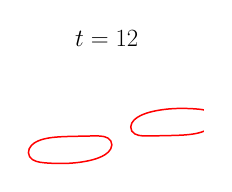
\begin{tikzpicture}[scale=0.36]

\begin{axis}[
  xmin = -6,
  xmax = 2,
  ymin = -2,
  ymax = 2,
  axis equal = true,
  hide axis,
  title = {\Huge$t=12$}
  ]

\addplot [mark=none,red,line width=1.5] table{
1.0896e+00 8.3914e-02
1.1473e+00 8.7321e-02
1.2094e+00 9.1519e-02
1.2790e+00 9.6982e-02
1.3584e+00 1.0433e-01
1.4485e+00 1.1438e-01
1.5496e+00 1.2823e-01
1.6614e+00 1.4744e-01
1.7828e+00 1.7420e-01
1.9122e+00 2.1161e-01
2.0463e+00 2.6411e-01
2.1794e+00 3.3777e-01
2.3011e+00 4.4003e-01
2.3921e+00 5.7642e-01
2.4242e+00 7.4070e-01
2.3752e+00 9.0283e-01
2.2557e+00 1.0251e+00
2.1001e+00 1.0972e+00
1.9339e+00 1.1347e+00
1.7676e+00 1.1549e+00
1.6048e+00 1.1674e+00
1.4475e+00 1.1759e+00
1.2969e+00 1.1814e+00
1.1545e+00 1.1840e+00
1.0213e+00 1.1839e+00
8.9820e-01 1.1814e+00
7.8604e-01 1.1769e+00
6.8524e-01 1.1711e+00
5.9581e-01 1.1644e+00
5.1725e-01 1.1574e+00
4.4833e-01 1.1503e+00
3.8690e-01 1.1433e+00
3.2966e-01 1.1361e+00
2.7241e-01 1.1283e+00
2.1094e-01 1.1192e+00
1.4203e-01 1.1080e+00
6.3637e-02 1.0940e+00
-2.5214e-02 1.0764e+00
-1.2476e-01 1.0542e+00
-2.3456e-01 1.0262e+00
-3.5370e-01 9.9069e-01
-4.8045e-01 9.4546e-01
-6.1215e-01 8.8727e-01
-7.4413e-01 8.1152e-01
-8.6796e-01 7.1170e-01
-9.6691e-01 5.8061e-01
-1.0112e+00 4.1904e-01
-9.6919e-01 2.5518e-01
-8.4733e-01 1.3585e-01
-6.8709e-01 7.5285e-02
-5.1822e-01 5.3156e-02
-3.5079e-01 4.8692e-02
-1.8760e-01 5.0418e-02
-3.0136e-02 5.3747e-02
1.2039e-01 5.7078e-02
2.6276e-01 6.0082e-02
3.9597e-01 6.2762e-02
5.1903e-01 6.5260e-02
6.3128e-01 6.7702e-02
7.3224e-01 7.0186e-02
8.2193e-01 7.2755e-02
9.0080e-01 7.5406e-02
9.7009e-01 7.8126e-02
1.0319e+00 8.0925e-02
1.0896e+00 8.3914e-02
};

\addplot [mark=none,red,line width=1.5] table{
-3.1297e+00 -1.0361e+00
-3.0724e+00 -1.0283e+00
-3.0109e+00 -1.0192e+00
-2.9420e+00 -1.0080e+00
-2.8636e+00 -9.9402e-01
-2.7748e+00 -9.7642e-01
-2.6752e+00 -9.5422e-01
-2.5654e+00 -9.2619e-01
-2.4463e+00 -8.9069e-01
-2.3195e+00 -8.4546e-01
-2.1879e+00 -7.8727e-01
-2.0559e+00 -7.1152e-01
-1.9320e+00 -6.1170e-01
-1.8331e+00 -4.8061e-01
-1.7888e+00 -3.1904e-01
-1.8308e+00 -1.5518e-01
-1.9527e+00 -3.5847e-02
-2.1129e+00 2.4716e-02
-2.2818e+00 4.6844e-02
-2.4492e+00 5.1308e-02
-2.6124e+00 4.9582e-02
-2.7699e+00 4.6253e-02
-2.9204e+00 4.2922e-02
-3.0628e+00 3.9918e-02
-3.1960e+00 3.7238e-02
-3.3190e+00 3.4740e-02
-3.4313e+00 3.2298e-02
-3.5322e+00 2.9814e-02
-3.6219e+00 2.7245e-02
-3.7008e+00 2.4594e-02
-3.7701e+00 2.1874e-02
-3.8319e+00 1.9075e-02
-3.8896e+00 1.6086e-02
-3.9473e+00 1.2679e-02
-4.0094e+00 8.4808e-03
-4.0790e+00 3.0180e-03
-4.1584e+00 -4.3319e-03
-4.2485e+00 -1.4377e-02
-4.3496e+00 -2.8233e-02
-4.4614e+00 -4.7442e-02
-4.5828e+00 -7.4195e-02
-4.7122e+00 -1.1161e-01
-4.8463e+00 -1.6411e-01
-4.9794e+00 -2.3777e-01
-5.1011e+00 -3.4003e-01
-5.1921e+00 -4.7642e-01
-5.2242e+00 -6.4070e-01
-5.1752e+00 -8.0283e-01
-5.0557e+00 -9.2508e-01
-4.9001e+00 -9.9721e-01
-4.7339e+00 -1.0347e+00
-4.5676e+00 -1.0549e+00
-4.4048e+00 -1.0674e+00
-4.2475e+00 -1.0759e+00
-4.0969e+00 -1.0814e+00
-3.9545e+00 -1.0840e+00
-3.8213e+00 -1.0839e+00
-3.6982e+00 -1.0814e+00
-3.5860e+00 -1.0769e+00
-3.4852e+00 -1.0711e+00
-3.3958e+00 -1.0644e+00
-3.3173e+00 -1.0574e+00
-3.2483e+00 -1.0503e+00
-3.1869e+00 -1.0433e+00
-3.1297e+00 -1.0361e+00
};

\end{axis}
\end{tikzpicture}


%\fi
%\end{tabular}
%\begin{tabular}{cc}
%\ifInputs
%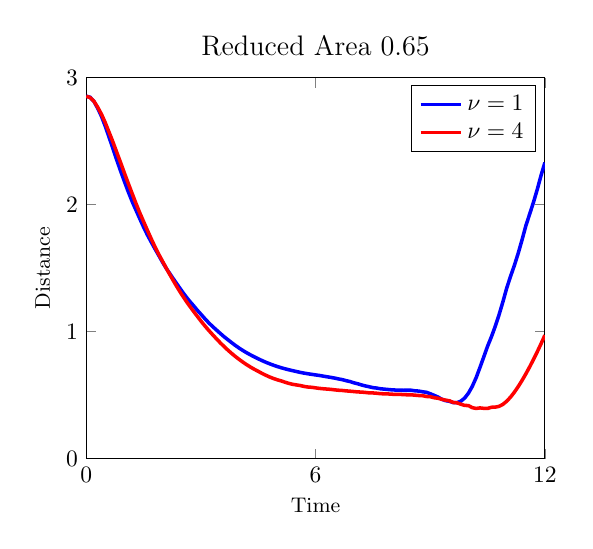
\begin{tikzpicture}[scale=0.85]

\begin{axis}[
  xmin = 0,
  xmax = 12, 
  ymin = 0,
  ymax = 3,
  xtick = {0,6,12,18,24},
  xticklabels = {$0$,$6$,$12$,$18$,$24$},
  ytick = {0,1,2,3},
  yticklabels = {$0$,$1$,$2$,$3$},
  xlabel = {Time},
  ylabel = {Distance},
  label style = {font=\small},
  legend entries = {$\nu=1$,$\nu=4$},
  title = {\large{Reduced Area 0.65}}
  ]

\addplot [mark=none,blue,line width=1.5] table{
0.0000e+00 2.8531e+00
1.0000e-01 2.8450e+00
2.0000e-01 2.8130e+00
3.0000e-01 2.7588e+00
4.0000e-01 2.6942e+00
5.0000e-01 2.6158e+00
6.0000e-01 2.5286e+00
7.0000e-01 2.4404e+00
8.0000e-01 2.3502e+00
9.0000e-01 2.2643e+00
1.0000e+00 2.1815e+00
1.1000e+00 2.1009e+00
1.2000e+00 2.0258e+00
1.3000e+00 1.9573e+00
1.4000e+00 1.8897e+00
1.5000e+00 1.8236e+00
1.6000e+00 1.7618e+00
1.7000e+00 1.7057e+00
1.8000e+00 1.6511e+00
1.9000e+00 1.5987e+00
2.0000e+00 1.5448e+00
2.1000e+00 1.4954e+00
2.2000e+00 1.4504e+00
2.3000e+00 1.4064e+00
2.4000e+00 1.3633e+00
2.5000e+00 1.3202e+00
2.6000e+00 1.2790e+00
2.7000e+00 1.2412e+00
2.8000e+00 1.2068e+00
2.9000e+00 1.1704e+00
3.0000e+00 1.1371e+00
3.1000e+00 1.1031e+00
3.2000e+00 1.0710e+00
3.3000e+00 1.0415e+00
3.4000e+00 1.0145e+00
3.5000e+00 9.8739e-01
3.6000e+00 9.6133e-01
3.7000e+00 9.3737e-01
3.8000e+00 9.1418e-01
3.9000e+00 8.9130e-01
4.0000e+00 8.7022e-01
4.1000e+00 8.5077e-01
4.2000e+00 8.3282e-01
4.3000e+00 8.1622e-01
4.4000e+00 8.0084e-01
4.5000e+00 7.8585e-01
4.6000e+00 7.7159e-01
4.7000e+00 7.5845e-01
4.8000e+00 7.4634e-01
4.9000e+00 7.3520e-01
5.0000e+00 7.2496e-01
5.1000e+00 7.1559e-01
5.2000e+00 7.0706e-01
5.3000e+00 6.9938e-01
5.4000e+00 6.9246e-01
5.5000e+00 6.8553e-01
5.6000e+00 6.7890e-01
5.7000e+00 6.7299e-01
5.8000e+00 6.6790e-01
5.9000e+00 6.6341e-01
6.0000e+00 6.5881e-01
6.1000e+00 6.5449e-01
6.2000e+00 6.4944e-01
6.3000e+00 6.4415e-01
6.4000e+00 6.3916e-01
6.5000e+00 6.3382e-01
6.6000e+00 6.2731e-01
6.7000e+00 6.2176e-01
6.8000e+00 6.1347e-01
6.9000e+00 6.0690e-01
7.0000e+00 5.9685e-01
7.1000e+00 5.8949e-01
7.2000e+00 5.8011e-01
7.3000e+00 5.7244e-01
7.4000e+00 5.6590e-01
7.5000e+00 5.5863e-01
7.6000e+00 5.5544e-01
7.7000e+00 5.4959e-01
7.8000e+00 5.4687e-01
7.9000e+00 5.4405e-01
8.0000e+00 5.4138e-01
8.1000e+00 5.3964e-01
8.2000e+00 5.3852e-01
8.3000e+00 5.3803e-01
8.4000e+00 5.3819e-01
8.5000e+00 5.3816e-01
8.6000e+00 5.3370e-01
8.7000e+00 5.3159e-01
8.8000e+00 5.2603e-01
8.9000e+00 5.2205e-01
9.0000e+00 5.1079e-01
9.1000e+00 4.9818e-01
9.2000e+00 4.8514e-01
9.3000e+00 4.6758e-01
9.4000e+00 4.5670e-01
9.5000e+00 4.5139e-01
9.6000e+00 4.4093e-01
9.7000e+00 4.4051e-01
9.8000e+00 4.5179e-01
9.9000e+00 4.7630e-01
1.0000e+01 5.1515e-01
1.0100e+01 5.6864e-01
1.0200e+01 6.3619e-01
1.0300e+01 7.1663e-01
1.0400e+01 8.0004e-01
1.0500e+01 8.8447e-01
1.0600e+01 9.5850e-01
1.0700e+01 1.0405e+00
1.0800e+01 1.1320e+00
1.0900e+01 1.2330e+00
1.1000e+01 1.3416e+00
1.1100e+01 1.4339e+00
1.1200e+01 1.5199e+00
1.1300e+01 1.6153e+00
1.1400e+01 1.7201e+00
1.1500e+01 1.8316e+00
1.1600e+01 1.9242e+00
1.1700e+01 2.0169e+00
1.1800e+01 2.1190e+00
1.1900e+01 2.2301e+00
1.2000e+01 2.3305e+00
};

\addplot [mark=none,red,line width=1.5] table{
0.0000e+00 2.8531e+00
1.0000e-01 2.8425e+00
2.0000e-01 2.8141e+00
3.0000e-01 2.7663e+00
4.0000e-01 2.7108e+00
5.0000e-01 2.6437e+00
6.0000e-01 2.5684e+00
7.0000e-01 2.4921e+00
8.0000e-01 2.4106e+00
9.0000e-01 2.3303e+00
1.0000e+00 2.2477e+00
1.1000e+00 2.1671e+00
1.2000e+00 2.0883e+00
1.3000e+00 2.0102e+00
1.4000e+00 1.9360e+00
1.5000e+00 1.8667e+00
1.6000e+00 1.7981e+00
1.7000e+00 1.7310e+00
1.8000e+00 1.6668e+00
1.9000e+00 1.6071e+00
2.0000e+00 1.5516e+00
2.1000e+00 1.4956e+00
2.2000e+00 1.4425e+00
2.3000e+00 1.3902e+00
2.4000e+00 1.3394e+00
2.5000e+00 1.2914e+00
2.6000e+00 1.2462e+00
2.7000e+00 1.2034e+00
2.8000e+00 1.1629e+00
2.9000e+00 1.1230e+00
3.0000e+00 1.0838e+00
3.1000e+00 1.0467e+00
3.2000e+00 1.0115e+00
3.3000e+00 9.7804e-01
3.4000e+00 9.4557e-01
3.5000e+00 9.1400e-01
3.6000e+00 8.8418e-01
3.7000e+00 8.5605e-01
3.8000e+00 8.2954e-01
3.9000e+00 8.0461e-01
4.0000e+00 7.8123e-01
4.1000e+00 7.5938e-01
4.2000e+00 7.3905e-01
4.3000e+00 7.2026e-01
4.4000e+00 7.0303e-01
4.5000e+00 6.8709e-01
4.6000e+00 6.7088e-01
4.7000e+00 6.5600e-01
4.8000e+00 6.4254e-01
4.9000e+00 6.3061e-01
5.0000e+00 6.2035e-01
5.1000e+00 6.1191e-01
5.2000e+00 6.0149e-01
5.3000e+00 5.9231e-01
5.4000e+00 5.8509e-01
5.5000e+00 5.8006e-01
5.6000e+00 5.7532e-01
5.7000e+00 5.6822e-01
5.8000e+00 5.6362e-01
5.9000e+00 5.6131e-01
6.0000e+00 5.5688e-01
6.1000e+00 5.5282e-01
6.2000e+00 5.4992e-01
6.3000e+00 5.4744e-01
6.4000e+00 5.4511e-01
6.5000e+00 5.4129e-01
6.6000e+00 5.3829e-01
6.7000e+00 5.3633e-01
6.8000e+00 5.3323e-01
6.9000e+00 5.3073e-01
7.0000e+00 5.2811e-01
7.1000e+00 5.2498e-01
7.2000e+00 5.2383e-01
7.3000e+00 5.2099e-01
7.4000e+00 5.1770e-01
7.5000e+00 5.1693e-01
7.6000e+00 5.1455e-01
7.7000e+00 5.1113e-01
7.8000e+00 5.1003e-01
7.9000e+00 5.0897e-01
8.0000e+00 5.0693e-01
8.1000e+00 5.0519e-01
8.2000e+00 5.0612e-01
8.3000e+00 5.0335e-01
8.4000e+00 5.0253e-01
8.5000e+00 5.0236e-01
8.6000e+00 4.9943e-01
8.7000e+00 4.9680e-01
8.8000e+00 4.9512e-01
8.9000e+00 4.8914e-01
9.0000e+00 4.8753e-01
9.1000e+00 4.7934e-01
9.2000e+00 4.7539e-01
9.3000e+00 4.6720e-01
9.4000e+00 4.6023e-01
9.5000e+00 4.5526e-01
9.6000e+00 4.4234e-01
9.7000e+00 4.3923e-01
9.8000e+00 4.2839e-01
9.9000e+00 4.1876e-01
1.0000e+01 4.1755e-01
1.0100e+01 4.0116e-01
1.0200e+01 3.9493e-01
1.0300e+01 3.9913e-01
1.0400e+01 3.9578e-01
1.0500e+01 3.9483e-01
1.0600e+01 4.0415e-01
1.0700e+01 4.0543e-01
1.0800e+01 4.1119e-01
1.0900e+01 4.2691e-01
1.1000e+01 4.5154e-01
1.1100e+01 4.8379e-01
1.1200e+01 5.2237e-01
1.1300e+01 5.6617e-01
1.1400e+01 6.1434e-01
1.1500e+01 6.6627e-01
1.1600e+01 7.2153e-01
1.1700e+01 7.7985e-01
1.1800e+01 8.4102e-01
1.1900e+01 9.0494e-01
1.2000e+01 9.7152e-01
};

\end{axis}

%\draw[gray,thin] (0,0) grid +(3,4);

\end{tikzpicture}

 &
%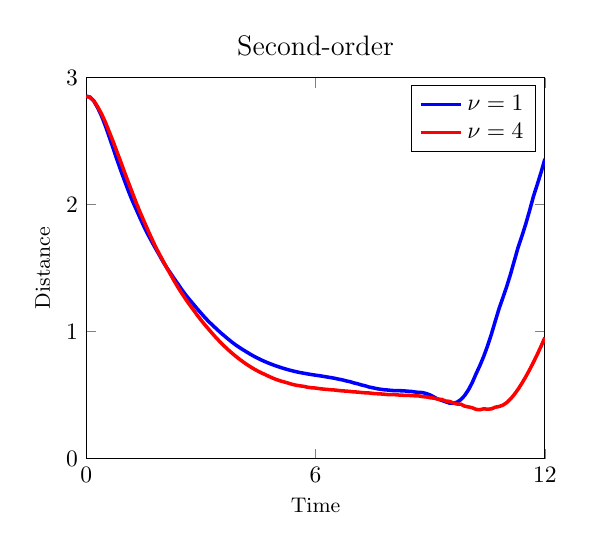
\begin{tikzpicture}[scale=0.85]

\begin{axis}[
  xmin = 0,
  xmax = 12, 
  ymin = 0,
  ymax = 3,
  xtick = {0,6,12,18,24},
  xticklabels = {$0$,$6$,$12$,$18$,$24$},
  ytick = {0,1,2,3},
  yticklabels = {$0$,$1$,$2$,$3$},
  xlabel = {Time},
  ylabel = {Distance},
  label style = {font=\small},
  legend entries = {$\nu=1$,$\nu=4$},
  title = {\large{Second-order}}
  ]

\addplot [mark=none,blue,line width=1.5] table{
0.0000e+00 2.8531e+00
1.0000e-01 2.8459e+00
2.0000e-01 2.8150e+00
3.0000e-01 2.7618e+00
4.0000e-01 2.6984e+00
5.0000e-01 2.6213e+00
6.0000e-01 2.5351e+00
7.0000e-01 2.4476e+00
8.0000e-01 2.3582e+00
9.0000e-01 2.2728e+00
1.0000e+00 2.1905e+00
1.1000e+00 2.1103e+00
1.2000e+00 2.0355e+00
1.3000e+00 1.9674e+00
1.4000e+00 1.9002e+00
1.5000e+00 1.8341e+00
1.6000e+00 1.7726e+00
1.7000e+00 1.7169e+00
1.8000e+00 1.6621e+00
1.9000e+00 1.6095e+00
2.0000e+00 1.5558e+00
2.1000e+00 1.5069e+00
2.2000e+00 1.4623e+00
2.3000e+00 1.4176e+00
2.4000e+00 1.3750e+00
2.5000e+00 1.3308e+00
2.6000e+00 1.2900e+00
2.7000e+00 1.2528e+00
2.8000e+00 1.2169e+00
2.9000e+00 1.1810e+00
3.0000e+00 1.1467e+00
3.1000e+00 1.1122e+00
3.2000e+00 1.0806e+00
3.3000e+00 1.0516e+00
3.4000e+00 1.0235e+00
3.5000e+00 9.9555e-01
3.6000e+00 9.6990e-01
3.7000e+00 9.4447e-01
3.8000e+00 9.1990e-01
3.9000e+00 8.9729e-01
4.0000e+00 8.7646e-01
4.1000e+00 8.5727e-01
4.2000e+00 8.3889e-01
4.3000e+00 8.2069e-01
4.4000e+00 8.0389e-01
4.5000e+00 7.8836e-01
4.6000e+00 7.7399e-01
4.7000e+00 7.6066e-01
4.8000e+00 7.4828e-01
4.9000e+00 7.3678e-01
5.0000e+00 7.2609e-01
5.1000e+00 7.1615e-01
5.2000e+00 7.0694e-01
5.3000e+00 6.9843e-01
5.4000e+00 6.9062e-01
5.5000e+00 6.8355e-01
5.6000e+00 6.7723e-01
5.7000e+00 6.7169e-01
5.8000e+00 6.6643e-01
5.9000e+00 6.6147e-01
6.0000e+00 6.5671e-01
6.1000e+00 6.5251e-01
6.2000e+00 6.4755e-01
6.3000e+00 6.4248e-01
6.4000e+00 6.3766e-01
6.5000e+00 6.3233e-01
6.6000e+00 6.2559e-01
6.7000e+00 6.1991e-01
6.8000e+00 6.1168e-01
6.9000e+00 6.0564e-01
7.0000e+00 5.9606e-01
7.1000e+00 5.8925e-01
7.2000e+00 5.7994e-01
7.3000e+00 5.7310e-01
7.4000e+00 5.6330e-01
7.5000e+00 5.5746e-01
7.6000e+00 5.5075e-01
7.7000e+00 5.4596e-01
7.8000e+00 5.4184e-01
7.9000e+00 5.3963e-01
8.0000e+00 5.3644e-01
8.1000e+00 5.3496e-01
8.2000e+00 5.3443e-01
8.3000e+00 5.3382e-01
8.4000e+00 5.3079e-01
8.5000e+00 5.2881e-01
8.6000e+00 5.2446e-01
8.7000e+00 5.2131e-01
8.8000e+00 5.1985e-01
8.9000e+00 5.1183e-01
9.0000e+00 5.0074e-01
9.1000e+00 4.8441e-01
9.2000e+00 4.6857e-01
9.3000e+00 4.5855e-01
9.4000e+00 4.4758e-01
9.5000e+00 4.3716e-01
9.6000e+00 4.3565e-01
9.7000e+00 4.4427e-01
9.8000e+00 4.6420e-01
9.9000e+00 4.9638e-01
1.0000e+01 5.4129e-01
1.0100e+01 5.9878e-01
1.0200e+01 6.6819e-01
1.0300e+01 7.3307e-01
1.0400e+01 8.0537e-01
1.0500e+01 8.8755e-01
1.0600e+01 9.7948e-01
1.0700e+01 1.0808e+00
1.0800e+01 1.1802e+00
1.0900e+01 1.2663e+00
1.1000e+01 1.3540e+00
1.1100e+01 1.4514e+00
1.1200e+01 1.5579e+00
1.1300e+01 1.6642e+00
1.1400e+01 1.7530e+00
1.1500e+01 1.8484e+00
1.1600e+01 1.9530e+00
1.1700e+01 2.0642e+00
1.1800e+01 2.1576e+00
1.1900e+01 2.2540e+00
1.2000e+01 2.3596e+00
};

\addplot [mark=none,red,line width=1.5] table{
0.0000e+00 2.8531e+00
1.0000e-01 2.8436e+00
2.0000e-01 2.8163e+00
3.0000e-01 2.7697e+00
4.0000e-01 2.7153e+00
5.0000e-01 2.6495e+00
6.0000e-01 2.5753e+00
7.0000e-01 2.4999e+00
8.0000e-01 2.4193e+00
9.0000e-01 2.3395e+00
1.0000e+00 2.2574e+00
1.1000e+00 2.1773e+00
1.2000e+00 2.0987e+00
1.3000e+00 2.0207e+00
1.4000e+00 1.9468e+00
1.5000e+00 1.8772e+00
1.6000e+00 1.8089e+00
1.7000e+00 1.7414e+00
1.8000e+00 1.6775e+00
1.9000e+00 1.6180e+00
2.0000e+00 1.5623e+00
2.1000e+00 1.5059e+00
2.2000e+00 1.4530e+00
2.3000e+00 1.3997e+00
2.4000e+00 1.3490e+00
2.5000e+00 1.3011e+00
2.6000e+00 1.2559e+00
2.7000e+00 1.2133e+00
2.8000e+00 1.1726e+00
2.9000e+00 1.1313e+00
3.0000e+00 1.0921e+00
3.1000e+00 1.0550e+00
3.2000e+00 1.0197e+00
3.3000e+00 9.8477e-01
3.4000e+00 9.5119e-01
3.5000e+00 9.1939e-01
3.6000e+00 8.8931e-01
3.7000e+00 8.6086e-01
3.8000e+00 8.3399e-01
3.9000e+00 8.0865e-01
4.0000e+00 7.8480e-01
4.1000e+00 7.6242e-01
4.2000e+00 7.4148e-01
4.3000e+00 7.2199e-01
4.4000e+00 7.0398e-01
4.5000e+00 6.8748e-01
4.6000e+00 6.7254e-01
4.7000e+00 6.5882e-01
4.8000e+00 6.4436e-01
4.9000e+00 6.3130e-01
5.0000e+00 6.1979e-01
5.1000e+00 6.0997e-01
5.2000e+00 6.0200e-01
5.3000e+00 5.9289e-01
5.4000e+00 5.8404e-01
5.5000e+00 5.7723e-01
5.6000e+00 5.7269e-01
5.7000e+00 5.6817e-01
5.8000e+00 5.6152e-01
5.9000e+00 5.5752e-01
6.0000e+00 5.5557e-01
6.1000e+00 5.5086e-01
6.2000e+00 5.4739e-01
6.3000e+00 5.4478e-01
6.4000e+00 5.4214e-01
6.5000e+00 5.3995e-01
6.6000e+00 5.3635e-01
6.7000e+00 5.3300e-01
6.8000e+00 5.3169e-01
6.9000e+00 5.2872e-01
7.0000e+00 5.2520e-01
7.1000e+00 5.2397e-01
7.2000e+00 5.2039e-01
7.3000e+00 5.1799e-01
7.4000e+00 5.1663e-01
7.5000e+00 5.1304e-01
7.6000e+00 5.1086e-01
7.7000e+00 5.0937e-01
7.8000e+00 5.0660e-01
7.9000e+00 5.0402e-01
8.0000e+00 5.0398e-01
8.1000e+00 5.0273e-01
8.2000e+00 4.9997e-01
8.3000e+00 4.9859e-01
8.4000e+00 4.9859e-01
8.5000e+00 4.9606e-01
8.6000e+00 4.9453e-01
8.7000e+00 4.9327e-01
8.8000e+00 4.8812e-01
8.9000e+00 4.8529e-01
9.0000e+00 4.7916e-01
9.1000e+00 4.7582e-01
9.2000e+00 4.6801e-01
9.3000e+00 4.6597e-01
9.4000e+00 4.5352e-01
9.5000e+00 4.5058e-01
9.6000e+00 4.3858e-01
9.7000e+00 4.2949e-01
9.8000e+00 4.2872e-01
9.9000e+00 4.1300e-01
1.0000e+01 4.0712e-01
1.0100e+01 4.0027e-01
1.0200e+01 3.8742e-01
1.0300e+01 3.8477e-01
1.0400e+01 3.9230e-01
1.0500e+01 3.8881e-01
1.0600e+01 3.9169e-01
1.0700e+01 4.0444e-01
1.0800e+01 4.1011e-01
1.0900e+01 4.2064e-01
1.1000e+01 4.4074e-01
1.1100e+01 4.6929e-01
1.1200e+01 5.0504e-01
1.1300e+01 5.4683e-01
1.1400e+01 5.9371e-01
1.1500e+01 6.4495e-01
1.1600e+01 7.0001e-01
1.1700e+01 7.5853e-01
1.1800e+01 8.2025e-01
1.1900e+01 8.8498e-01
1.2000e+01 9.5258e-01
};

\end{axis}

%\draw[gray,thin] (0,0) grid +(3,4);

\end{tikzpicture}


%\fi
%\end{tabular}
%\mcaption{Two vesicles of reduced Area $0.65$ are submerged in a shear
%flow.  The vesicles in the top row have no viscosity contrast and the
%vesicles in the second row have a viscosity contrast of 4.  The bottom
%plots show the distance between the vesicles for both viscosity
%contrasts with first- and second-order time stepping.  Implicit
%vesicle-vesicle interactions are used for all the simulations.  The gap
%sizes of the first- and second-order methods differ by 1.7\% for $\nu=1$
%and by 2.3\% for $\nu=4$.}{f:shear:reducedArea1} 
%\end{figure}
%
%
%\begin{figure}[htp]
%\centering
%\begin{tabular}{m{1cm}CCCCC}
%\ifInputs
%$\nu=1$ &
%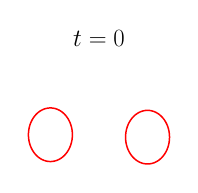
\begin{tikzpicture}[scale=0.36]

\begin{axis}[
  xmin = -6,
  xmax = 2,
  ymin = -2,
  ymax = 2,
  axis equal = true,
  hide axis,
  title = {\Huge$t=0$}
  ]

\addplot [mark=none,red,line width=1.5] table{
-4.0000e+00 1.2044e+00
-4.0888e+00 1.1991e+00
-4.1766e+00 1.1832e+00
-4.2628e+00 1.1568e+00
-4.3465e+00 1.1203e+00
-4.4268e+00 1.0740e+00
-4.5031e+00 1.0183e+00
-4.5744e+00 9.5370e-01
-4.6403e+00 8.8092e-01
-4.6999e+00 8.0062e-01
-4.7529e+00 7.1357e-01
-4.7986e+00 6.2061e-01
-4.8366e+00 5.2263e-01
-4.8665e+00 4.2059e-01
-4.8881e+00 3.1546e-01
-4.9011e+00 2.0825e-01
-4.9055e+00 1.0000e-01
-4.9011e+00 -8.2491e-03
-4.8881e+00 -1.1546e-01
-4.8665e+00 -2.2059e-01
-4.8366e+00 -3.2263e-01
-4.7986e+00 -4.2061e-01
-4.7529e+00 -5.1357e-01
-4.6999e+00 -6.0062e-01
-4.6403e+00 -6.8092e-01
-4.5744e+00 -7.5370e-01
-4.5031e+00 -8.1827e-01
-4.4268e+00 -8.7398e-01
-4.3465e+00 -9.2032e-01
-4.2628e+00 -9.5683e-01
-4.1766e+00 -9.8317e-01
-4.0888e+00 -9.9907e-01
-4.0000e+00 -1.0044e+00
-3.9112e+00 -9.9907e-01
-3.8234e+00 -9.8317e-01
-3.7372e+00 -9.5683e-01
-3.6535e+00 -9.2032e-01
-3.5732e+00 -8.7398e-01
-3.4969e+00 -8.1827e-01
-3.4256e+00 -7.5370e-01
-3.3597e+00 -6.8092e-01
-3.3001e+00 -6.0062e-01
-3.2471e+00 -5.1357e-01
-3.2014e+00 -4.2061e-01
-3.1634e+00 -3.2263e-01
-3.1335e+00 -2.2059e-01
-3.1119e+00 -1.1546e-01
-3.0989e+00 -8.2491e-03
-3.0945e+00 1.0000e-01
-3.0989e+00 2.0825e-01
-3.1119e+00 3.1546e-01
-3.1335e+00 4.2059e-01
-3.1634e+00 5.2263e-01
-3.2014e+00 6.2061e-01
-3.2471e+00 7.1357e-01
-3.3001e+00 8.0062e-01
-3.3597e+00 8.8092e-01
-3.4256e+00 9.5370e-01
-3.4969e+00 1.0183e+00
-3.5732e+00 1.0740e+00
-3.6535e+00 1.1203e+00
-3.7372e+00 1.1568e+00
-3.8234e+00 1.1832e+00
-3.9112e+00 1.1991e+00
-4.0000e+00 1.2044e+00
};

\addplot [mark=none,red,line width=1.5] table{
6.7624e-17 1.1044e+00
-8.8752e-02 1.0991e+00
-1.7665e-01 1.0832e+00
-2.6285e-01 1.0568e+00
-3.4651e-01 1.0203e+00
-4.2684e-01 9.7398e-01
-5.0306e-01 9.1827e-01
-5.7443e-01 8.5370e-01
-6.4027e-01 7.8092e-01
-6.9994e-01 7.0062e-01
-7.5288e-01 6.1357e-01
-7.9856e-01 5.2061e-01
-8.3655e-01 4.2263e-01
-8.6649e-01 3.2059e-01
-8.8808e-01 2.1546e-01
-9.0112e-01 1.0825e-01
-9.0548e-01 1.2307e-16
-9.0112e-01 -1.0825e-01
-8.8808e-01 -2.1546e-01
-8.6649e-01 -3.2059e-01
-8.3655e-01 -4.2263e-01
-7.9856e-01 -5.2061e-01
-7.5288e-01 -6.1357e-01
-6.9994e-01 -7.0062e-01
-6.4027e-01 -7.8092e-01
-5.7443e-01 -8.5370e-01
-5.0306e-01 -9.1827e-01
-4.2684e-01 -9.7398e-01
-3.4651e-01 -1.0203e+00
-2.6285e-01 -1.0568e+00
-1.7665e-01 -1.0832e+00
-8.8752e-02 -1.0991e+00
-1.7851e-16 -1.1044e+00
8.8752e-02 -1.0991e+00
1.7665e-01 -1.0832e+00
2.6285e-01 -1.0568e+00
3.4651e-01 -1.0203e+00
4.2684e-01 -9.7398e-01
5.0306e-01 -9.1827e-01
5.7443e-01 -8.5370e-01
6.4027e-01 -7.8092e-01
6.9994e-01 -7.0062e-01
7.5288e-01 -6.1357e-01
7.9856e-01 -5.2061e-01
8.3655e-01 -4.2263e-01
8.6649e-01 -3.2059e-01
8.8808e-01 -2.1546e-01
9.0112e-01 -1.0825e-01
9.0548e-01 -2.5832e-16
9.0112e-01 1.0825e-01
8.8808e-01 2.1546e-01
8.6649e-01 3.2059e-01
8.3655e-01 4.2263e-01
7.9856e-01 5.2061e-01
7.5288e-01 6.1357e-01
6.9994e-01 7.0062e-01
6.4027e-01 7.8092e-01
5.7443e-01 8.5370e-01
5.0306e-01 9.1827e-01
4.2684e-01 9.7398e-01
3.4651e-01 1.0203e+00
2.6285e-01 1.0568e+00
1.7665e-01 1.0832e+00
8.8752e-02 1.0991e+00
6.7624e-17 1.1044e+00
};

\end{axis}
\end{tikzpicture}

 &
%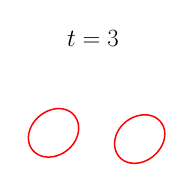
\begin{tikzpicture}[scale=0.36]

\begin{axis}[
  xmin = -6,
  xmax = 2,
  ymin = -2,
  ymax = 2,
  axis equal = true,
  hide axis,
  title = {\Huge$t=3$}
  ]

\addplot [mark=none,red,line width=1.5] table{
-2.5977e+00 4.8832e-01
-2.6136e+00 5.7651e-01
-2.6390e+00 6.6290e-01
-2.6741e+00 7.4667e-01
-2.7193e+00 8.2673e-01
-2.7749e+00 9.0180e-01
-2.8407e+00 9.7040e-01
-2.9162e+00 1.0310e+00
-3.0006e+00 1.0823e+00
-3.0927e+00 1.1232e+00
-3.1908e+00 1.1528e+00
-3.2934e+00 1.1708e+00
-3.3989e+00 1.1772e+00
-3.5058e+00 1.1723e+00
-3.6126e+00 1.1566e+00
-3.7181e+00 1.1307e+00
-3.8212e+00 1.0955e+00
-3.9209e+00 1.0515e+00
-4.0164e+00 9.9983e-01
-4.1070e+00 9.4111e-01
-4.1920e+00 8.7622e-01
-4.2709e+00 8.0594e-01
-4.3432e+00 7.3105e-01
-4.4087e+00 6.5227e-01
-4.4670e+00 5.7028e-01
-4.5179e+00 4.8570e-01
-4.5613e+00 3.9909e-01
-4.5968e+00 3.1095e-01
-4.6245e+00 2.2175e-01
-4.6441e+00 1.3188e-01
-4.6553e+00 4.1744e-02
-4.6579e+00 -4.8257e-02
-4.6515e+00 -1.3765e-01
-4.6357e+00 -2.2587e-01
-4.6101e+00 -3.1216e-01
-4.5742e+00 -3.9558e-01
-4.5279e+00 -4.7501e-01
-4.4711e+00 -5.4913e-01
-4.4041e+00 -6.1654e-01
-4.3275e+00 -6.7589e-01
-4.2424e+00 -7.2598e-01
-4.1500e+00 -7.6586e-01
-4.0517e+00 -7.9493e-01
-3.9490e+00 -8.1287e-01
-3.8435e+00 -8.1970e-01
-3.7366e+00 -8.1563e-01
-3.6297e+00 -8.0109e-01
-3.5238e+00 -7.7659e-01
-3.4202e+00 -7.4276e-01
-3.3199e+00 -7.0027e-01
-3.2237e+00 -6.4983e-01
-3.1325e+00 -5.9217e-01
-3.0469e+00 -5.2805e-01
-2.9676e+00 -4.5823e-01
-2.8951e+00 -3.8347e-01
-2.8299e+00 -3.0454e-01
-2.7721e+00 -2.2217e-01
-2.7221e+00 -1.3705e-01
-2.6801e+00 -4.9854e-02
-2.6460e+00 3.8837e-02
-2.6199e+00 1.2850e-01
-2.6019e+00 2.1867e-01
-2.5921e+00 3.0896e-01
-2.5906e+00 3.9898e-01
-2.5977e+00 4.8832e-01
};

\addplot [mark=none,red,line width=1.5] table{
9.5150e-01 2.3765e-01
9.3570e-01 3.2587e-01
9.1006e-01 4.1216e-01
8.7420e-01 4.9558e-01
8.2788e-01 5.7501e-01
7.7107e-01 6.4913e-01
7.0408e-01 7.1654e-01
6.2752e-01 7.7589e-01
5.4241e-01 8.2598e-01
4.4998e-01 8.6586e-01
3.5169e-01 8.9493e-01
2.4904e-01 9.1287e-01
1.4355e-01 9.1970e-01
3.6642e-02 9.1563e-01
-7.0337e-02 9.0109e-01
-1.7617e-01 8.7659e-01
-2.7976e-01 8.4276e-01
-3.8009e-01 8.0027e-01
-4.7628e-01 7.4983e-01
-5.6751e-01 6.9217e-01
-6.5308e-01 6.2805e-01
-7.3237e-01 5.5823e-01
-8.0486e-01 4.8347e-01
-8.7014e-01 4.0454e-01
-9.2788e-01 3.2217e-01
-9.7786e-01 2.3705e-01
-1.0199e+00 1.4985e-01
-1.0540e+00 6.1163e-02
-1.0801e+00 -2.8498e-02
-1.0981e+00 -1.1867e-01
-1.1079e+00 -2.0896e-01
-1.1094e+00 -2.9898e-01
-1.1023e+00 -3.8832e-01
-1.0864e+00 -4.7651e-01
-1.0610e+00 -5.6290e-01
-1.0259e+00 -6.4667e-01
-9.8069e-01 -7.2673e-01
-9.2511e-01 -8.0180e-01
-8.5931e-01 -8.7040e-01
-7.8377e-01 -9.3104e-01
-6.9936e-01 -9.8234e-01
-6.0735e-01 -1.0232e+00
-5.0922e-01 -1.0528e+00
-4.0659e-01 -1.0708e+00
-3.0107e-01 -1.0772e+00
-1.9420e-01 -1.0723e+00
-8.7390e-02 -1.0566e+00
1.8121e-02 -1.0307e+00
1.2122e-01 -9.9546e-01
2.2094e-01 -9.5155e-01
3.1645e-01 -8.9983e-01
4.0700e-01 -8.4111e-01
4.9198e-01 -7.7622e-01
5.7087e-01 -7.0594e-01
6.4323e-01 -6.3105e-01
7.0870e-01 -5.5227e-01
7.6701e-01 -4.7028e-01
8.1793e-01 -3.8570e-01
8.6126e-01 -2.9909e-01
8.9685e-01 -2.1095e-01
9.2452e-01 -1.2175e-01
9.4408e-01 -3.1882e-02
9.5531e-01 5.8256e-02
9.5790e-01 1.4826e-01
9.5150e-01 2.3765e-01
};

\end{axis}
\end{tikzpicture}

 &
%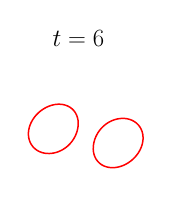
\begin{tikzpicture}[scale=0.36]

\begin{axis}[
  xmin = -6,
  xmax = 2,
  ymin = -2,
  ymax = 2,
  axis equal = true,
  hide axis,
  title = {\Huge$t=6$}
  ]

\addplot [mark=none,red,line width=1.5] table{
-2.5082e+00 -4.1872e-01
-2.4390e+00 -3.6122e-01
-2.3736e+00 -2.9869e-01
-2.3123e+00 -2.3109e-01
-2.2552e+00 -1.5840e-01
-2.2026e+00 -8.0595e-02
-2.1548e+00 2.2781e-03
-2.1124e+00 9.0108e-02
-2.0759e+00 1.8269e-01
-2.0463e+00 2.7970e-01
-2.0244e+00 3.8068e-01
-2.0115e+00 4.8492e-01
-2.0089e+00 5.9144e-01
-2.0179e+00 6.9888e-01
-2.0400e+00 8.0538e-01
-2.0762e+00 9.0861e-01
-2.1269e+00 1.0059e+00
-2.1915e+00 1.0944e+00
-2.2686e+00 1.1717e+00
-2.3559e+00 1.2358e+00
-2.4508e+00 1.2861e+00
-2.5504e+00 1.3223e+00
-2.6524e+00 1.3452e+00
-2.7545e+00 1.3558e+00
-2.8554e+00 1.3556e+00
-2.9539e+00 1.3458e+00
-3.0493e+00 1.3276e+00
-3.1412e+00 1.3021e+00
-3.2293e+00 1.2702e+00
-3.3135e+00 1.2327e+00
-3.3940e+00 1.1900e+00
-3.4709e+00 1.1424e+00
-3.5442e+00 1.0902e+00
-3.6140e+00 1.0335e+00
-3.6804e+00 9.7208e-01
-3.7433e+00 9.0594e-01
-3.8025e+00 8.3489e-01
-3.8576e+00 7.5876e-01
-3.9081e+00 6.7745e-01
-3.9531e+00 5.9093e-01
-3.9919e+00 4.9929e-01
-4.0233e+00 4.0282e-01
-4.0460e+00 3.0204e-01
-4.0588e+00 1.9779e-01
-4.0601e+00 9.1271e-02
-4.0487e+00 -1.5902e-02
-4.0236e+00 -1.2169e-01
-3.9843e+00 -2.2370e-01
-3.9308e+00 -3.1938e-01
-3.8640e+00 -4.0624e-01
-3.7857e+00 -4.8218e-01
-3.6979e+00 -5.4575e-01
-3.6031e+00 -5.9620e-01
-3.5039e+00 -6.3352e-01
-3.4024e+00 -6.5821e-01
-3.3004e+00 -6.7117e-01
-3.1995e+00 -6.7345e-01
-3.1008e+00 -6.6616e-01
-3.0050e+00 -6.5035e-01
-2.9126e+00 -6.2696e-01
-2.8239e+00 -5.9679e-01
-2.7391e+00 -5.6047e-01
-2.6582e+00 -5.1849e-01
-2.5813e+00 -4.7117e-01
-2.5082e+00 -4.1872e-01
};

\addplot [mark=none,red,line width=1.5] table{
1.4417e-01 -9.9023e-01
2.1402e-01 -9.3347e-01
2.8044e-01 -8.7208e-01
3.4335e-01 -8.0594e-01
4.0253e-01 -7.3489e-01
4.5762e-01 -6.5876e-01
5.0806e-01 -5.7745e-01
5.5313e-01 -4.9093e-01
5.9191e-01 -3.9929e-01
6.2329e-01 -3.0282e-01
6.4602e-01 -2.0204e-01
6.5875e-01 -9.7791e-02
6.6009e-01 8.7287e-03
6.4872e-01 1.1590e-01
6.2364e-01 2.2169e-01
5.8429e-01 3.2370e-01
5.3080e-01 4.1938e-01
4.6404e-01 5.0624e-01
3.8567e-01 5.8218e-01
2.9788e-01 6.4575e-01
2.0313e-01 6.9620e-01
1.0388e-01 7.3352e-01
2.3623e-03 7.5821e-01
-9.9573e-02 7.7117e-01
-2.0045e-01 7.7345e-01
-2.9919e-01 7.6616e-01
-3.9501e-01 7.5035e-01
-4.8741e-01 7.2696e-01
-5.7608e-01 6.9679e-01
-6.6088e-01 6.6047e-01
-7.4176e-01 6.1849e-01
-8.1873e-01 5.7117e-01
-8.9182e-01 5.1872e-01
-9.6105e-01 4.6122e-01
-1.0264e+00 3.9869e-01
-1.0877e+00 3.3109e-01
-1.1448e+00 2.5840e-01
-1.1974e+00 1.8060e-01
-1.2452e+00 9.7722e-02
-1.2876e+00 9.8920e-03
-1.3241e+00 -8.2690e-02
-1.3537e+00 -1.7970e-01
-1.3756e+00 -2.8068e-01
-1.3885e+00 -3.8492e-01
-1.3911e+00 -4.9144e-01
-1.3821e+00 -5.9888e-01
-1.3600e+00 -7.0538e-01
-1.3238e+00 -8.0861e-01
-1.2731e+00 -9.0588e-01
-1.2085e+00 -9.9439e-01
-1.1314e+00 -1.0717e+00
-1.0441e+00 -1.1358e+00
-9.4922e-01 -1.1861e+00
-8.4958e-01 -1.2223e+00
-7.4765e-01 -1.2452e+00
-6.4546e-01 -1.2558e+00
-5.4457e-01 -1.2556e+00
-4.4605e-01 -1.2458e+00
-3.5066e-01 -1.2276e+00
-2.5881e-01 -1.2021e+00
-1.7072e-01 -1.1702e+00
-8.6457e-02 -1.1327e+00
-5.9586e-03 -1.0900e+00
7.0878e-02 -1.0424e+00
1.4417e-01 -9.9023e-01
};

\end{axis}
\end{tikzpicture}

 &
%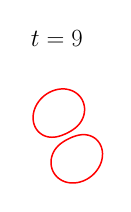
\begin{tikzpicture}[scale=0.36]

\begin{axis}[
  xmin = -6,
  xmax = 2,
  ymin = -2,
  ymax = 2,
  axis equal = true,
  hide axis,
  title = {\Huge$t=9$}
  ]

\addplot [mark=none,red,line width=1.5] table{
-2.6374e+00 1.2421e-01
-2.5592e+00 7.8773e-02
-2.4757e+00 4.2962e-02
-2.3878e+00 1.7103e-02
-2.2963e+00 1.4030e-03
-2.2022e+00 -4.0951e-03
-2.1063e+00 4.2682e-04
-2.0095e+00 1.4495e-02
-1.9123e+00 3.7313e-02
-1.8152e+00 6.7827e-02
-1.7184e+00 1.0489e-01
-1.6219e+00 1.4755e-01
-1.5261e+00 1.9525e-01
-1.4315e+00 2.4808e-01
-1.3391e+00 3.0661e-01
-1.2504e+00 3.7171e-01
-1.1671e+00 4.4413e-01
-1.0911e+00 5.2414e-01
-1.0241e+00 6.1135e-01
-9.6752e-01 7.0480e-01
-9.2231e-01 8.0310e-01
-8.8901e-01 9.0466e-01
-8.6787e-01 1.0078e+00
-8.5884e-01 1.1110e+00
-8.6169e-01 1.2127e+00
-8.7598e-01 1.3114e+00
-9.0110e-01 1.4060e+00
-9.3632e-01 1.4953e+00
-9.8080e-01 1.5785e+00
-1.0337e+00 1.6548e+00
-1.0940e+00 1.7238e+00
-1.1611e+00 1.7852e+00
-1.2340e+00 1.8387e+00
-1.3122e+00 1.8842e+00
-1.3950e+00 1.9215e+00
-1.4820e+00 1.9507e+00
-1.5725e+00 1.9715e+00
-1.6660e+00 1.9838e+00
-1.7620e+00 1.9875e+00
-1.8598e+00 1.9824e+00
-1.9587e+00 1.9684e+00
-2.0579e+00 1.9454e+00
-2.1565e+00 1.9135e+00
-2.2538e+00 1.8728e+00
-2.3487e+00 1.8234e+00
-2.4402e+00 1.7656e+00
-2.5275e+00 1.6999e+00
-2.6095e+00 1.6267e+00
-2.6854e+00 1.5466e+00
-2.7542e+00 1.4605e+00
-2.8151e+00 1.3690e+00
-2.8673e+00 1.2731e+00
-2.9103e+00 1.1738e+00
-2.9433e+00 1.0721e+00
-2.9661e+00 9.6930e-01
-2.9783e+00 8.6641e-01
-2.9798e+00 7.6469e-01
-2.9706e+00 6.6531e-01
-2.9508e+00 5.6946e-01
-2.9207e+00 4.7824e-01
-2.8809e+00 3.9270e-01
-2.8320e+00 3.1377e-01
-2.7746e+00 2.4226e-01
-2.7094e+00 1.7888e-01
-2.6374e+00 1.2421e-01
};

\addplot [mark=none,red,line width=1.5] table{
-1.8660e+00 -1.7387e+00
-1.7878e+00 -1.7842e+00
-1.7050e+00 -1.8215e+00
-1.6180e+00 -1.8507e+00
-1.5275e+00 -1.8715e+00
-1.4340e+00 -1.8838e+00
-1.3380e+00 -1.8875e+00
-1.2402e+00 -1.8824e+00
-1.1413e+00 -1.8684e+00
-1.0421e+00 -1.8454e+00
-9.4346e-01 -1.8135e+00
-8.4621e-01 -1.7728e+00
-7.5132e-01 -1.7234e+00
-6.5975e-01 -1.6656e+00
-5.7248e-01 -1.5999e+00
-4.9046e-01 -1.5267e+00
-4.1461e-01 -1.4466e+00
-3.4583e-01 -1.3605e+00
-2.8494e-01 -1.2690e+00
-2.3269e-01 -1.1731e+00
-1.8974e-01 -1.0738e+00
-1.5666e-01 -9.7215e-01
-1.3386e-01 -8.6930e-01
-1.2165e-01 -7.6641e-01
-1.2018e-01 -6.6469e-01
-1.2943e-01 -5.6531e-01
-1.4924e-01 -4.6946e-01
-1.7928e-01 -3.7824e-01
-2.1907e-01 -2.9270e-01
-2.6801e-01 -2.1377e-01
-3.2543e-01 -1.4226e-01
-3.9056e-01 -7.8876e-02
-4.6263e-01 -2.4215e-02
-5.4081e-01 2.1227e-02
-6.2429e-01 5.7038e-02
-7.1221e-01 8.2897e-02
-8.0367e-01 9.8597e-02
-8.9778e-01 1.0410e-01
-9.9366e-01 9.9573e-02
-1.0905e+00 8.5505e-02
-1.1877e+00 6.2687e-02
-1.2848e+00 3.2173e-02
-1.3816e+00 -4.8930e-03
-1.4781e+00 -4.7545e-02
-1.5739e+00 -9.5255e-02
-1.6685e+00 -1.4808e-01
-1.7609e+00 -2.0661e-01
-1.8496e+00 -2.7171e-01
-1.9329e+00 -3.4413e-01
-2.0089e+00 -4.2414e-01
-2.0759e+00 -5.1135e-01
-2.1325e+00 -6.0480e-01
-2.1777e+00 -7.0310e-01
-2.2110e+00 -8.0466e-01
-2.2321e+00 -9.0783e-01
-2.2412e+00 -1.0110e+00
-2.2383e+00 -1.1127e+00
-2.2240e+00 -1.2114e+00
-2.1989e+00 -1.3060e+00
-2.1637e+00 -1.3953e+00
-2.1192e+00 -1.4785e+00
-2.0663e+00 -1.5548e+00
-2.0060e+00 -1.6238e+00
-1.9389e+00 -1.6852e+00
-1.8660e+00 -1.7387e+00
};

\end{axis}
\end{tikzpicture}

 &
%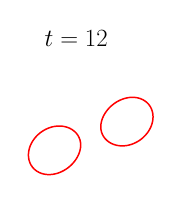
\begin{tikzpicture}[scale=0.36]

\begin{axis}[
  xmin = -6,
  xmax = 2,
  ymin = -2,
  ymax = 2,
  axis equal = true,
  hide axis,
  title = {\Huge$t=12$}
  ]

\addplot [mark=none,red,line width=1.5] table{
-6.3844e-01 1.2046e+00
-6.9949e-01 1.1364e+00
-7.5633e-01 1.0640e+00
-8.0872e-01 9.8729e-01
-8.5621e-01 9.0600e-01
-8.9812e-01 8.1999e-01
-9.3348e-01 7.2920e-01
-9.6102e-01 6.3378e-01
-9.7916e-01 5.3420e-01
-9.8610e-01 4.3135e-01
-9.7999e-01 3.2666e-01
-9.5925e-01 2.2218e-01
-9.2299e-01 1.2048e-01
-8.7127e-01 2.4308e-02
-8.0519e-01 -6.3788e-02
-7.2658e-01 -1.4181e-01
-6.3773e-01 -2.0841e-01
-5.4100e-01 -2.6284e-01
-4.3869e-01 -3.0483e-01
-3.3293e-01 -3.3454e-01
-2.2557e-01 -3.5244e-01
-1.1826e-01 -3.5920e-01
-1.2331e-02 -3.5569e-01
9.1146e-02 -3.4284e-01
1.9135e-01 -3.2158e-01
2.8770e-01 -2.9284e-01
3.7979e-01 -2.5744e-01
4.6740e-01 -2.1611e-01
5.5042e-01 -1.6947e-01
6.2882e-01 -1.1799e-01
7.0267e-01 -6.1985e-02
7.7201e-01 -1.6670e-03
8.3687e-01 6.2896e-02
8.9722e-01 1.3173e-01
9.5293e-01 2.0493e-01
1.0037e+00 2.8264e-01
1.0491e+00 3.6499e-01
1.0885e+00 4.5201e-01
1.1210e+00 5.4367e-01
1.1456e+00 6.3970e-01
1.1610e+00 7.3958e-01
1.1660e+00 8.4247e-01
1.1590e+00 9.4709e-01
1.1389e+00 1.0517e+00
1.1048e+00 1.1542e+00
1.0561e+00 1.2520e+00
9.9338e-01 1.3425e+00
9.1762e-01 1.4233e+00
8.3071e-01 1.4924e+00
7.3497e-01 1.5485e+00
6.3293e-01 1.5911e+00
5.2703e-01 1.6202e+00
4.1947e-01 1.6367e+00
3.1207e-01 1.6413e+00
2.0627e-01 1.6354e+00
1.0316e-01 1.6200e+00
3.5368e-03 1.5963e+00
-9.2089e-02 1.5653e+00
-1.8339e-01 1.5281e+00
-2.7022e-01 1.4853e+00
-3.5255e-01 1.4376e+00
-4.3043e-01 1.3854e+00
-5.0396e-01 1.3291e+00
-5.7327e-01 1.2688e+00
-6.3844e-01 1.2046e+00
};

\addplot [mark=none,red,line width=1.5] table{
-3.6369e+00 3.7104e-02
-3.6972e+00 -3.1729e-02
-3.7529e+00 -1.0493e-01
-3.8037e+00 -1.8264e-01
-3.8491e+00 -2.6499e-01
-3.8885e+00 -3.5201e-01
-3.9210e+00 -4.4367e-01
-3.9456e+00 -5.3970e-01
-3.9610e+00 -6.3958e-01
-3.9660e+00 -7.4247e-01
-3.9590e+00 -8.4709e-01
-3.9389e+00 -9.5171e-01
-3.9048e+00 -1.0542e+00
-3.8561e+00 -1.1520e+00
-3.7934e+00 -1.2425e+00
-3.7176e+00 -1.3233e+00
-3.6307e+00 -1.3924e+00
-3.5350e+00 -1.4485e+00
-3.4329e+00 -1.4911e+00
-3.3270e+00 -1.5202e+00
-3.2195e+00 -1.5367e+00
-3.1121e+00 -1.5413e+00
-3.0063e+00 -1.5354e+00
-2.9032e+00 -1.5200e+00
-2.8035e+00 -1.4963e+00
-2.7079e+00 -1.4653e+00
-2.6166e+00 -1.4281e+00
-2.5298e+00 -1.3853e+00
-2.4475e+00 -1.3376e+00
-2.3696e+00 -1.2854e+00
-2.2960e+00 -1.2291e+00
-2.2267e+00 -1.1688e+00
-2.1616e+00 -1.1046e+00
-2.1005e+00 -1.0364e+00
-2.0437e+00 -9.6401e-01
-1.9913e+00 -8.8729e-01
-1.9438e+00 -8.0600e-01
-1.9019e+00 -7.1999e-01
-1.8665e+00 -6.2920e-01
-1.8390e+00 -5.3378e-01
-1.8208e+00 -4.3420e-01
-1.8139e+00 -3.3135e-01
-1.8200e+00 -2.2666e-01
-1.8407e+00 -1.2218e-01
-1.8770e+00 -2.0478e-02
-1.9287e+00 7.5692e-02
-1.9948e+00 1.6379e-01
-2.0734e+00 2.4181e-01
-2.1623e+00 3.0841e-01
-2.2590e+00 3.6284e-01
-2.3613e+00 4.0483e-01
-2.4671e+00 4.3454e-01
-2.5744e+00 4.5244e-01
-2.6817e+00 4.5920e-01
-2.7877e+00 4.5569e-01
-2.8911e+00 4.4284e-01
-2.9914e+00 4.2158e-01
-3.0877e+00 3.9284e-01
-3.1798e+00 3.5744e-01
-3.2674e+00 3.1611e-01
-3.3504e+00 2.6947e-01
-3.4288e+00 2.1799e-01
-3.5027e+00 1.6199e-01
-3.5720e+00 1.0167e-01
-3.6369e+00 3.7104e-02
};

\end{axis}
\end{tikzpicture}


%\fi
%\end{tabular}
%\begin{tabular}{m{1cm}CCCCC}
%\ifInputs
%$\nu=4$ &
%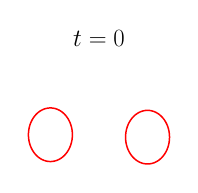
\begin{tikzpicture}[scale=0.36]

\begin{axis}[
  xmin = -6,
  xmax = 2,
  ymin = -2,
  ymax = 2,
  axis equal = true,
  hide axis,
  title = {\Huge$t=0$}
  ]

\addplot [mark=none,red,line width=1.5] table{
-4.0000e+00 1.2044e+00
-4.0888e+00 1.1991e+00
-4.1766e+00 1.1832e+00
-4.2628e+00 1.1568e+00
-4.3465e+00 1.1203e+00
-4.4268e+00 1.0740e+00
-4.5031e+00 1.0183e+00
-4.5744e+00 9.5370e-01
-4.6403e+00 8.8092e-01
-4.6999e+00 8.0062e-01
-4.7529e+00 7.1357e-01
-4.7986e+00 6.2061e-01
-4.8366e+00 5.2263e-01
-4.8665e+00 4.2059e-01
-4.8881e+00 3.1546e-01
-4.9011e+00 2.0825e-01
-4.9055e+00 1.0000e-01
-4.9011e+00 -8.2491e-03
-4.8881e+00 -1.1546e-01
-4.8665e+00 -2.2059e-01
-4.8366e+00 -3.2263e-01
-4.7986e+00 -4.2061e-01
-4.7529e+00 -5.1357e-01
-4.6999e+00 -6.0062e-01
-4.6403e+00 -6.8092e-01
-4.5744e+00 -7.5370e-01
-4.5031e+00 -8.1827e-01
-4.4268e+00 -8.7398e-01
-4.3465e+00 -9.2032e-01
-4.2628e+00 -9.5683e-01
-4.1766e+00 -9.8317e-01
-4.0888e+00 -9.9907e-01
-4.0000e+00 -1.0044e+00
-3.9112e+00 -9.9907e-01
-3.8234e+00 -9.8317e-01
-3.7372e+00 -9.5683e-01
-3.6535e+00 -9.2032e-01
-3.5732e+00 -8.7398e-01
-3.4969e+00 -8.1827e-01
-3.4256e+00 -7.5370e-01
-3.3597e+00 -6.8092e-01
-3.3001e+00 -6.0062e-01
-3.2471e+00 -5.1357e-01
-3.2014e+00 -4.2061e-01
-3.1634e+00 -3.2263e-01
-3.1335e+00 -2.2059e-01
-3.1119e+00 -1.1546e-01
-3.0989e+00 -8.2491e-03
-3.0945e+00 1.0000e-01
-3.0989e+00 2.0825e-01
-3.1119e+00 3.1546e-01
-3.1335e+00 4.2059e-01
-3.1634e+00 5.2263e-01
-3.2014e+00 6.2061e-01
-3.2471e+00 7.1357e-01
-3.3001e+00 8.0062e-01
-3.3597e+00 8.8092e-01
-3.4256e+00 9.5370e-01
-3.4969e+00 1.0183e+00
-3.5732e+00 1.0740e+00
-3.6535e+00 1.1203e+00
-3.7372e+00 1.1568e+00
-3.8234e+00 1.1832e+00
-3.9112e+00 1.1991e+00
-4.0000e+00 1.2044e+00
};

\addplot [mark=none,red,line width=1.5] table{
6.7624e-17 1.1044e+00
-8.8752e-02 1.0991e+00
-1.7665e-01 1.0832e+00
-2.6285e-01 1.0568e+00
-3.4651e-01 1.0203e+00
-4.2684e-01 9.7398e-01
-5.0306e-01 9.1827e-01
-5.7443e-01 8.5370e-01
-6.4027e-01 7.8092e-01
-6.9994e-01 7.0062e-01
-7.5288e-01 6.1357e-01
-7.9856e-01 5.2061e-01
-8.3655e-01 4.2263e-01
-8.6649e-01 3.2059e-01
-8.8808e-01 2.1546e-01
-9.0112e-01 1.0825e-01
-9.0548e-01 1.2307e-16
-9.0112e-01 -1.0825e-01
-8.8808e-01 -2.1546e-01
-8.6649e-01 -3.2059e-01
-8.3655e-01 -4.2263e-01
-7.9856e-01 -5.2061e-01
-7.5288e-01 -6.1357e-01
-6.9994e-01 -7.0062e-01
-6.4027e-01 -7.8092e-01
-5.7443e-01 -8.5370e-01
-5.0306e-01 -9.1827e-01
-4.2684e-01 -9.7398e-01
-3.4651e-01 -1.0203e+00
-2.6285e-01 -1.0568e+00
-1.7665e-01 -1.0832e+00
-8.8752e-02 -1.0991e+00
-1.7851e-16 -1.1044e+00
8.8752e-02 -1.0991e+00
1.7665e-01 -1.0832e+00
2.6285e-01 -1.0568e+00
3.4651e-01 -1.0203e+00
4.2684e-01 -9.7398e-01
5.0306e-01 -9.1827e-01
5.7443e-01 -8.5370e-01
6.4027e-01 -7.8092e-01
6.9994e-01 -7.0062e-01
7.5288e-01 -6.1357e-01
7.9856e-01 -5.2061e-01
8.3655e-01 -4.2263e-01
8.6649e-01 -3.2059e-01
8.8808e-01 -2.1546e-01
9.0112e-01 -1.0825e-01
9.0548e-01 -2.5832e-16
9.0112e-01 1.0825e-01
8.8808e-01 2.1546e-01
8.6649e-01 3.2059e-01
8.3655e-01 4.2263e-01
7.9856e-01 5.2061e-01
7.5288e-01 6.1357e-01
6.9994e-01 7.0062e-01
6.4027e-01 7.8092e-01
5.7443e-01 8.5370e-01
5.0306e-01 9.1827e-01
4.2684e-01 9.7398e-01
3.4651e-01 1.0203e+00
2.6285e-01 1.0568e+00
1.7665e-01 1.0832e+00
8.8752e-02 1.0991e+00
6.7624e-17 1.1044e+00
};

\end{axis}
\end{tikzpicture}

 &
%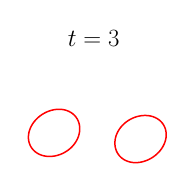
\begin{tikzpicture}[scale=0.36]

\begin{axis}[
  xmin = -6,
  xmax = 2,
  ymin = -2,
  ymax = 2,
  axis equal = true,
  hide axis,
  title = {\Huge$t=3$}
  ]

\addplot [mark=none,red,line width=1.5] table{
-2.5859e+00 4.9427e-01
-2.6062e+00 5.8147e-01
-2.6363e+00 6.6622e-01
-2.6764e+00 7.4760e-01
-2.7267e+00 8.2453e-01
-2.7870e+00 8.9578e-01
-2.8569e+00 9.6008e-01
-2.9357e+00 1.0163e+00
-3.0225e+00 1.0633e+00
-3.1160e+00 1.1004e+00
-3.2149e+00 1.1272e+00
-3.3178e+00 1.1434e+00
-3.4234e+00 1.1490e+00
-3.5302e+00 1.1443e+00
-3.6371e+00 1.1296e+00
-3.7430e+00 1.1055e+00
-3.8468e+00 1.0724e+00
-3.9475e+00 1.0309e+00
-4.0443e+00 9.8168e-01
-4.1364e+00 9.2543e-01
-4.2231e+00 8.6281e-01
-4.3037e+00 7.9452e-01
-4.3778e+00 7.2126e-01
-4.4447e+00 6.4372e-01
-4.5042e+00 5.6257e-01
-4.5558e+00 4.7845e-01
-4.5993e+00 3.9197e-01
-4.6344e+00 3.0372e-01
-4.6609e+00 2.1424e-01
-4.6786e+00 1.2407e-01
-4.6870e+00 3.3740e-02
-4.6861e+00 -5.6184e-02
-4.6755e+00 -1.4507e-01
-4.6549e+00 -2.3219e-01
-4.6241e+00 -3.1667e-01
-4.5830e+00 -3.9753e-01
-4.5316e+00 -4.7366e-01
-4.4701e+00 -5.4390e-01
-4.3992e+00 -6.0711e-01
-4.3196e+00 -6.6224e-01
-4.2324e+00 -7.0844e-01
-4.1387e+00 -7.4507e-01
-4.0397e+00 -7.7172e-01
-3.9369e+00 -7.8820e-01
-3.8314e+00 -7.9451e-01
-3.7245e+00 -7.9079e-01
-3.6174e+00 -7.7733e-01
-3.5113e+00 -7.5448e-01
-3.4071e+00 -7.2268e-01
-3.3058e+00 -6.8243e-01
-3.2085e+00 -6.3429e-01
-3.1159e+00 -5.7885e-01
-3.0288e+00 -5.1677e-01
-2.9480e+00 -4.4871e-01
-2.8741e+00 -3.7538e-01
-2.8075e+00 -2.9751e-01
-2.7488e+00 -2.1583e-01
-2.6982e+00 -1.3110e-01
-2.6560e+00 -4.3996e-02
-2.6223e+00 4.4800e-02
-2.5973e+00 1.3468e-01
-2.5810e+00 2.2509e-01
-2.5736e+00 3.1550e-01
-2.5751e+00 4.0541e-01
-2.5859e+00 4.9427e-01
};

\addplot [mark=none,red,line width=1.5] table{
9.7550e-01 2.4507e-01
9.5491e-01 3.3219e-01
9.2410e-01 4.1667e-01
8.8297e-01 4.9753e-01
8.3155e-01 5.7366e-01
7.7012e-01 6.4390e-01
6.9922e-01 7.0711e-01
6.1964e-01 7.6224e-01
5.3240e-01 8.0844e-01
4.3868e-01 8.4507e-01
3.3974e-01 8.7172e-01
2.3689e-01 8.8820e-01
1.3140e-01 8.9451e-01
2.4514e-02 8.9079e-01
-8.2575e-02 8.7733e-01
-1.8875e-01 8.5448e-01
-2.9295e-01 8.2268e-01
-3.9418e-01 7.8243e-01
-4.9152e-01 7.3429e-01
-5.8412e-01 6.7885e-01
-6.7117e-01 6.1677e-01
-7.5198e-01 5.4871e-01
-8.2593e-01 4.7538e-01
-8.9248e-01 3.9751e-01
-9.5122e-01 3.1583e-01
-1.0018e+00 2.3110e-01
-1.0440e+00 1.4400e-01
-1.0777e+00 5.5200e-02
-1.1027e+00 -3.4680e-02
-1.1190e+00 -1.2509e-01
-1.1264e+00 -2.1550e-01
-1.1249e+00 -3.0541e-01
-1.1141e+00 -3.9427e-01
-1.0938e+00 -4.8147e-01
-1.0637e+00 -5.6622e-01
-1.0236e+00 -6.4760e-01
-9.7331e-01 -7.2453e-01
-9.1303e-01 -7.9578e-01
-8.4311e-01 -8.6008e-01
-7.6426e-01 -9.1627e-01
-6.7747e-01 -9.6331e-01
-5.8396e-01 -1.0004e+00
-4.8505e-01 -1.0272e+00
-3.8216e-01 -1.0434e+00
-2.7664e-01 -1.0490e+00
-1.6980e-01 -1.0443e+00
-6.2876e-02 -1.0296e+00
4.3002e-02 -1.0055e+00
1.4679e-01 -9.7236e-01
2.4752e-01 -9.3088e-01
3.4434e-01 -8.8168e-01
4.3644e-01 -8.2543e-01
5.2311e-01 -7.6281e-01
6.0374e-01 -6.9452e-01
6.7777e-01 -6.2126e-01
7.4472e-01 -5.4372e-01
8.0418e-01 -4.6257e-01
8.5582e-01 -3.7845e-01
8.9933e-01 -2.9197e-01
9.3445e-01 -2.0372e-01
9.6094e-01 -1.1424e-01
9.7855e-01 -2.4072e-02
9.8704e-01 6.6260e-02
9.8611e-01 1.5618e-01
9.7550e-01 2.4507e-01
};

\end{axis}
\end{tikzpicture}

 &
%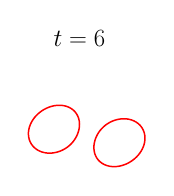
\begin{tikzpicture}[scale=0.36]

\begin{axis}[
  xmin = -6,
  xmax = 2,
  ymin = -2,
  ymax = 2,
  axis equal = true,
  hide axis,
  title = {\Huge$t=6$}
  ]

\addplot [mark=none,red,line width=1.5] table{
-2.4503e+00 -3.7535e-01
-2.3824e+00 -3.1632e-01
-2.3187e+00 -2.5231e-01
-2.2591e+00 -1.8323e-01
-2.2040e+00 -1.0904e-01
-2.1538e+00 -2.9703e-02
-2.1090e+00 5.4749e-02
-2.0703e+00 1.4419e-01
-2.0385e+00 2.3837e-01
-2.0146e+00 3.3686e-01
-2.0000e+00 4.3902e-01
-1.9961e+00 5.4384e-01
-2.0044e+00 6.4991e-01
-2.0262e+00 7.5529e-01
-2.0626e+00 8.5759e-01
-2.1137e+00 9.5407e-01
-2.1788e+00 1.0420e+00
-2.2565e+00 1.1190e+00
-2.3444e+00 1.1834e+00
-2.4399e+00 1.2345e+00
-2.5402e+00 1.2723e+00
-2.6432e+00 1.2974e+00
-2.7467e+00 1.3109e+00
-2.8494e+00 1.3138e+00
-2.9500e+00 1.3073e+00
-3.0479e+00 1.2925e+00
-3.1424e+00 1.2705e+00
-3.2333e+00 1.2420e+00
-3.3204e+00 1.2078e+00
-3.4037e+00 1.1684e+00
-3.4833e+00 1.1241e+00
-3.5592e+00 1.0752e+00
-3.6315e+00 1.0218e+00
-3.7002e+00 9.6380e-01
-3.7653e+00 9.0113e-01
-3.8267e+00 8.3361e-01
-3.8839e+00 7.6103e-01
-3.9364e+00 6.8322e-01
-3.9836e+00 6.0006e-01
-4.0245e+00 5.1156e-01
-4.0580e+00 4.1793e-01
-4.0826e+00 3.1963e-01
-4.0970e+00 2.1746e-01
-4.0997e+00 1.1262e-01
-4.0892e+00 6.7733e-03
-4.0646e+00 -9.7962e-02
-4.0254e+00 -1.9913e-01
-3.9717e+00 -2.9415e-01
-3.9046e+00 -3.8059e-01
-3.8258e+00 -4.5645e-01
-3.7375e+00 -5.2040e-01
-3.6423e+00 -5.7180e-01
-3.5423e+00 -6.1066e-01
-3.4398e+00 -6.3746e-01
-3.3365e+00 -6.5297e-01
-3.2339e+00 -6.5814e-01
-3.1331e+00 -6.5396e-01
-3.0350e+00 -6.4137e-01
-2.9400e+00 -6.2125e-01
-2.8487e+00 -5.9435e-01
-2.7611e+00 -5.6129e-01
-2.6775e+00 -5.2257e-01
-2.5978e+00 -4.7854e-01
-2.5221e+00 -4.2943e-01
-2.4503e+00 -3.7535e-01
};

\addplot [mark=none,red,line width=1.5] table{
2.3145e-01 -9.2179e-01
3.0019e-01 -8.6380e-01
3.6531e-01 -8.0113e-01
4.2665e-01 -7.3361e-01
4.8387e-01 -6.6103e-01
5.3644e-01 -5.8322e-01
5.8364e-01 -5.0006e-01
6.2454e-01 -4.1156e-01
6.5798e-01 -3.1793e-01
6.8263e-01 -2.1963e-01
6.9703e-01 -1.1746e-01
6.9968e-01 -1.2618e-02
6.8923e-01 9.3227e-02
6.6462e-01 1.9796e-01
6.2536e-01 2.9913e-01
5.7166e-01 3.9415e-01
5.0456e-01 4.8059e-01
4.2578e-01 5.5645e-01
3.3753e-01 6.2040e-01
2.4225e-01 6.7180e-01
1.4229e-01 7.1066e-01
3.9781e-02 7.3746e-01
-6.3488e-02 7.5297e-01
-1.6607e-01 7.5814e-01
-2.6685e-01 7.5396e-01
-3.6501e-01 7.4137e-01
-4.5997e-01 7.2125e-01
-5.5134e-01 6.9435e-01
-6.3889e-01 6.6129e-01
-7.2253e-01 6.2257e-01
-8.0221e-01 5.7854e-01
-8.7794e-01 5.2943e-01
-9.4973e-01 4.7535e-01
-1.0176e+00 4.1632e-01
-1.0813e+00 3.5231e-01
-1.1409e+00 2.8323e-01
-1.1960e+00 2.0904e-01
-1.2462e+00 1.2970e-01
-1.2910e+00 4.5251e-02
-1.3297e+00 -4.4188e-02
-1.3615e+00 -1.3837e-01
-1.3854e+00 -2.3686e-01
-1.4000e+00 -3.3902e-01
-1.4039e+00 -4.4384e-01
-1.3956e+00 -5.4991e-01
-1.3738e+00 -6.5529e-01
-1.3374e+00 -7.5759e-01
-1.2863e+00 -8.5407e-01
-1.2212e+00 -9.4198e-01
-1.1435e+00 -1.0190e+00
-1.0556e+00 -1.0834e+00
-9.6012e-01 -1.1345e+00
-8.5976e-01 -1.1723e+00
-7.5684e-01 -1.1974e+00
-6.5329e-01 -1.2109e+00
-5.5063e-01 -1.2138e+00
-4.4998e-01 -1.2073e+00
-3.5213e-01 -1.1925e+00
-2.5760e-01 -1.1705e+00
-1.6671e-01 -1.1420e+00
-7.9592e-02 -1.1078e+00
3.7182e-03 -1.0684e+00
8.3273e-02 -1.0241e+00
1.5916e-01 -9.7522e-01
2.3145e-01 -9.2179e-01
};

\end{axis}
\end{tikzpicture}

 &
%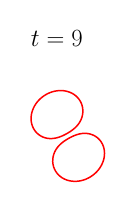
\begin{tikzpicture}[scale=0.36]

\begin{axis}[
  xmin = -6,
  xmax = 2,
  ymin = -2,
  ymax = 2,
  axis equal = true,
  hide axis,
  title = {\Huge$t=9$}
  ]

\addplot [mark=none,red,line width=1.5] table{
-2.5643e+00 1.7159e-03
-2.4789e+00 -2.7230e-02
-2.3903e+00 -4.6672e-02
-2.2994e+00 -5.6578e-02
-2.2067e+00 -5.6981e-02
-2.1130e+00 -4.8038e-02
-2.0188e+00 -3.0102e-02
-1.9247e+00 -3.7772e-03
-1.8309e+00 3.0086e-02
-1.7376e+00 7.0498e-02
-1.6448e+00 1.1655e-01
-1.5527e+00 1.6765e-01
-1.4618e+00 2.2374e-01
-1.3728e+00 2.8527e-01
-1.2872e+00 3.5308e-01
-1.2068e+00 4.2796e-01
-1.1336e+00 5.1031e-01
-1.0695e+00 5.9991e-01
-1.0162e+00 6.9589e-01
-9.7496e-01 7.9685e-01
-9.4660e-01 9.0109e-01
-9.3150e-01 1.0067e+00
-9.2964e-01 1.1119e+00
-9.4068e-01 1.2147e+00
-9.6395e-01 1.3135e+00
-9.9852e-01 1.4069e+00
-1.0433e+00 1.4936e+00
-1.0970e+00 1.5729e+00
-1.1584e+00 1.6442e+00
-1.2263e+00 1.7071e+00
-1.2997e+00 1.7617e+00
-1.3777e+00 1.8080e+00
-1.4595e+00 1.8460e+00
-1.5446e+00 1.8761e+00
-1.6326e+00 1.8982e+00
-1.7230e+00 1.9125e+00
-1.8155e+00 1.9190e+00
-1.9097e+00 1.9175e+00
-2.0051e+00 1.9080e+00
-2.1013e+00 1.8903e+00
-2.1976e+00 1.8643e+00
-2.2933e+00 1.8300e+00
-2.3877e+00 1.7872e+00
-2.4797e+00 1.7360e+00
-2.5685e+00 1.6766e+00
-2.6531e+00 1.6093e+00
-2.7324e+00 1.5344e+00
-2.8054e+00 1.4524e+00
-2.8710e+00 1.3640e+00
-2.9284e+00 1.2700e+00
-2.9765e+00 1.1714e+00
-3.0145e+00 1.0692e+00
-3.0418e+00 9.6469e-01
-3.0579e+00 8.5918e-01
-3.0624e+00 7.5409e-01
-3.0552e+00 6.5090e-01
-3.0366e+00 5.5107e-01
-3.0070e+00 4.5596e-01
-2.9671e+00 3.6682e-01
-2.9177e+00 2.8471e-01
-2.8599e+00 2.1046e-01
-2.7947e+00 1.4468e-01
-2.7231e+00 8.7806e-02
-2.6460e+00 4.0096e-02
-2.5643e+00 1.7159e-03
};

\addplot [mark=none,red,line width=1.5] table{
-1.6405e+00 -1.7460e+00
-1.5554e+00 -1.7761e+00
-1.4674e+00 -1.7982e+00
-1.3770e+00 -1.8125e+00
-1.2845e+00 -1.8190e+00
-1.1903e+00 -1.8175e+00
-1.0949e+00 -1.8080e+00
-9.9867e-01 -1.7903e+00
-9.0237e-01 -1.7643e+00
-8.0666e-01 -1.7300e+00
-7.1234e-01 -1.6872e+00
-6.2031e-01 -1.6360e+00
-5.3151e-01 -1.5766e+00
-4.4694e-01 -1.5093e+00
-3.6763e-01 -1.4344e+00
-2.9463e-01 -1.3524e+00
-2.2896e-01 -1.2640e+00
-1.7161e-01 -1.1700e+00
-1.2350e-01 -1.0714e+00
-8.5451e-02 -9.6921e-01
-5.8151e-02 -8.6469e-01
-4.2114e-02 -7.5918e-01
-3.7647e-02 -6.5409e-01
-4.4816e-02 -5.5090e-01
-6.3429e-02 -4.5107e-01
-9.3035e-02 -3.5596e-01
-1.3295e-01 -2.6682e-01
-1.8230e-01 -1.8471e-01
-2.4010e-01 -1.1046e-01
-3.0532e-01 -4.4683e-02
-3.7694e-01 1.2194e-02
-4.5401e-01 5.9904e-02
-5.3567e-01 9.8284e-02
-6.2114e-01 1.2723e-01
-7.0970e-01 1.4667e-01
-8.0064e-01 1.5658e-01
-8.9331e-01 1.5698e-01
-9.8703e-01 1.4804e-01
-1.0812e+00 1.3010e-01
-1.1753e+00 1.0378e-01
-1.2691e+00 6.9914e-02
-1.3624e+00 2.9502e-02
-1.4552e+00 -1.6548e-02
-1.5473e+00 -6.7650e-02
-1.6382e+00 -1.2374e-01
-1.7272e+00 -1.8527e-01
-1.8128e+00 -2.5308e-01
-1.8932e+00 -3.2796e-01
-1.9664e+00 -4.1031e-01
-2.0305e+00 -4.9991e-01
-2.0838e+00 -5.9589e-01
-2.1250e+00 -6.9685e-01
-2.1534e+00 -8.0109e-01
-2.1685e+00 -9.0673e-01
-2.1704e+00 -1.0119e+00
-2.1593e+00 -1.1147e+00
-2.1361e+00 -1.2135e+00
-2.1015e+00 -1.3069e+00
-2.0567e+00 -1.3936e+00
-2.0030e+00 -1.4729e+00
-1.9416e+00 -1.5442e+00
-1.8737e+00 -1.6071e+00
-1.8003e+00 -1.6617e+00
-1.7223e+00 -1.7080e+00
-1.6405e+00 -1.7460e+00
};

\end{axis}
\end{tikzpicture}

 &
%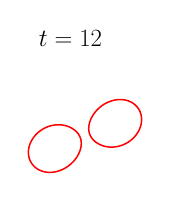
\begin{tikzpicture}[scale=0.36]

\begin{axis}[
  xmin = -6,
  xmax = 2,
  ymin = -2,
  ymax = 2,
  axis equal = true,
  hide axis,
  title = {\Huge$t=12$}
  ]

\addplot [mark=none,red,line width=1.5] table{
-1.0356e+00 9.6029e-01
-1.0855e+00 8.8378e-01
-1.1302e+00 8.0356e-01
-1.1692e+00 7.1946e-01
-1.2017e+00 6.3137e-01
-1.2267e+00 5.3928e-01
-1.2426e+00 4.4347e-01
-1.2474e+00 3.4464e-01
-1.2389e+00 2.4422e-01
-1.2150e+00 1.4442e-01
-1.1747e+00 4.8116e-02
-1.1186e+00 -4.1903e-02
-1.0487e+00 -1.2356e-01
-9.6728e-01 -1.9573e-01
-8.7677e-01 -2.5783e-01
-7.7921e-01 -3.0956e-01
-6.7637e-01 -3.5066e-01
-5.6988e-01 -3.8104e-01
-4.6127e-01 -4.0070e-01
-3.5196e-01 -4.0987e-01
-2.4328e-01 -4.0892e-01
-1.3638e-01 -3.9844e-01
-3.2259e-02 -3.7910e-01
6.8249e-02 -3.5164e-01
1.6451e-01 -3.1684e-01
2.5603e-01 -2.7544e-01
3.4250e-01 -2.2814e-01
4.2368e-01 -1.7555e-01
4.9947e-01 -1.1816e-01
5.6980e-01 -5.6370e-02
6.3467e-01 9.5559e-03
6.9400e-01 7.9454e-02
7.4772e-01 1.5328e-01
7.9561e-01 2.3102e-01
8.3735e-01 3.1274e-01
8.7242e-01 3.9842e-01
9.0015e-01 4.8799e-01
9.1965e-01 5.8122e-01
9.2990e-01 6.7763e-01
9.2976e-01 7.7643e-01
9.1811e-01 8.7647e-01
8.9391e-01 9.7620e-01
8.5646e-01 1.0737e+00
8.0553e-01 1.1668e+00
7.4145e-01 1.2532e+00
6.6519e-01 1.3309e+00
5.7831e-01 1.3980e+00
4.8273e-01 1.4533e+00
3.8062e-01 1.4961e+00
2.7411e-01 1.5263e+00
1.6522e-01 1.5442e+00
5.5735e-02 1.5504e+00
-5.2825e-02 1.5458e+00
-1.5923e-01 1.5313e+00
-2.6247e-01 1.5079e+00
-3.6181e-01 1.4765e+00
-4.5669e-01 1.4382e+00
-5.4675e-01 1.3939e+00
-6.3178e-01 1.3441e+00
-7.1167e-01 1.2897e+00
-7.8644e-01 1.2311e+00
-8.5614e-01 1.1687e+00
-9.2086e-01 1.1027e+00
-9.8067e-01 1.0332e+00
-1.0356e+00 9.6029e-01
};

\addplot [mark=none,red,line width=1.5] table{
-3.5477e+00 -5.3277e-02
-3.5956e+00 -1.3102e-01
-3.6373e+00 -2.1274e-01
-3.6724e+00 -2.9842e-01
-3.7001e+00 -3.8799e-01
-3.7196e+00 -4.8122e-01
-3.7299e+00 -5.7763e-01
-3.7298e+00 -6.7643e-01
-3.7181e+00 -7.7647e-01
-3.6939e+00 -8.7620e-01
-3.6565e+00 -9.7371e-01
-3.6055e+00 -1.0668e+00
-3.5414e+00 -1.1532e+00
-3.4652e+00 -1.2309e+00
-3.3783e+00 -1.2980e+00
-3.2827e+00 -1.3533e+00
-3.1806e+00 -1.3961e+00
-3.0741e+00 -1.4263e+00
-2.9652e+00 -1.4442e+00
-2.8557e+00 -1.4504e+00
-2.7472e+00 -1.4458e+00
-2.6408e+00 -1.4313e+00
-2.5375e+00 -1.4079e+00
-2.4382e+00 -1.3765e+00
-2.3433e+00 -1.3382e+00
-2.2532e+00 -1.2939e+00
-2.1682e+00 -1.2441e+00
-2.0883e+00 -1.1897e+00
-2.0136e+00 -1.1311e+00
-1.9439e+00 -1.0687e+00
-1.8791e+00 -1.0027e+00
-1.8193e+00 -9.3322e-01
-1.7644e+00 -8.6029e-01
-1.7145e+00 -7.8378e-01
-1.6698e+00 -7.0356e-01
-1.6308e+00 -6.1946e-01
-1.5983e+00 -5.3137e-01
-1.5733e+00 -4.3928e-01
-1.5574e+00 -3.4347e-01
-1.5526e+00 -2.4464e-01
-1.5611e+00 -1.4422e-01
-1.5850e+00 -4.4423e-02
-1.6253e+00 5.1884e-02
-1.6814e+00 1.4190e-01
-1.7513e+00 2.2356e-01
-1.8327e+00 2.9573e-01
-1.9232e+00 3.5783e-01
-2.0208e+00 4.0956e-01
-2.1236e+00 4.5066e-01
-2.2301e+00 4.8104e-01
-2.3387e+00 5.0070e-01
-2.4480e+00 5.0987e-01
-2.5567e+00 5.0892e-01
-2.6636e+00 4.9844e-01
-2.7677e+00 4.7910e-01
-2.8682e+00 4.5164e-01
-2.9645e+00 4.1684e-01
-3.0560e+00 3.7544e-01
-3.1425e+00 3.2814e-01
-3.2237e+00 2.7555e-01
-3.2995e+00 2.1816e-01
-3.3698e+00 1.5637e-01
-3.4347e+00 9.0444e-02
-3.4940e+00 2.0546e-02
-3.5477e+00 -5.3277e-02
};

\end{axis}
\end{tikzpicture}


%\fi
%\end{tabular}
%\begin{tabular}{cc}
%\ifInputs
%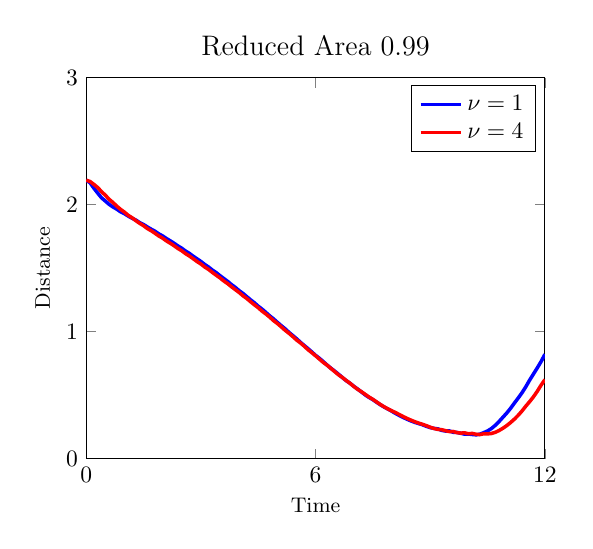
\begin{tikzpicture}[scale=0.85]

\begin{axis}[
  xmin = 0,
  xmax = 12, 
  ymin = 0,
  ymax = 3,
  xtick = {0,6,12,18,24},
  xticklabels = {$0$,$6$,$12$,$18$,$24$},
  ytick = {0,1,2,3},
  yticklabels = {$0$,$1$,$2$,$3$},
  xlabel = {Time},
  ylabel = {Distance},
  label style = {font=\small},
  legend entries = {$\nu=1$,$\nu=4$},
  title = {\large{Reduced Area 0.99}}
  ]

\addplot [mark=none,blue,line width=1.5] table{
0.0000e+00 2.1913e+00
1.0000e-01 2.1723e+00
2.0000e-01 2.1292e+00
3.0000e-01 2.0907e+00
4.0000e-01 2.0535e+00
5.0000e-01 2.0279e+00
6.0000e-01 2.0017e+00
7.0000e-01 1.9811e+00
8.0000e-01 1.9639e+00
9.0000e-01 1.9428e+00
1.0000e+00 1.9283e+00
1.1000e+00 1.9092e+00
1.2000e+00 1.8923e+00
1.3000e+00 1.8774e+00
1.4000e+00 1.8574e+00
1.5000e+00 1.8430e+00
1.6000e+00 1.8235e+00
1.7000e+00 1.8061e+00
1.8000e+00 1.7899e+00
1.9000e+00 1.7689e+00
2.0000e+00 1.7529e+00
2.1000e+00 1.7320e+00
2.2000e+00 1.7143e+00
2.3000e+00 1.6951e+00
2.4000e+00 1.6740e+00
2.5000e+00 1.6560e+00
2.6000e+00 1.6336e+00
2.7000e+00 1.6155e+00
2.8000e+00 1.5930e+00
2.9000e+00 1.5726e+00
3.0000e+00 1.5520e+00
3.1000e+00 1.5287e+00
3.2000e+00 1.5086e+00
3.3000e+00 1.4845e+00
3.4000e+00 1.4642e+00
3.5000e+00 1.4400e+00
3.6000e+00 1.4178e+00
3.7000e+00 1.3953e+00
3.8000e+00 1.3702e+00
3.9000e+00 1.3481e+00
4.0000e+00 1.3224e+00
4.1000e+00 1.3005e+00
4.2000e+00 1.2750e+00
4.3000e+00 1.2499e+00
4.4000e+00 1.2265e+00
4.5000e+00 1.1996e+00
4.6000e+00 1.1769e+00
4.7000e+00 1.1508e+00
4.8000e+00 1.1239e+00
4.9000e+00 1.1000e+00
5.0000e+00 1.0730e+00
5.1000e+00 1.0474e+00
5.2000e+00 1.0226e+00
5.3000e+00 9.9498e-01
5.4000e+00 9.6987e-01
5.5000e+00 9.4454e-01
5.6000e+00 9.1700e-01
5.7000e+00 8.9135e-01
5.8000e+00 8.6645e-01
5.9000e+00 8.4015e-01
6.0000e+00 8.1288e-01
6.1000e+00 7.8995e-01
6.2000e+00 7.6399e-01
6.3000e+00 7.3686e-01
6.4000e+00 7.1189e-01
6.5000e+00 6.8904e-01
6.6000e+00 6.6435e-01
6.7000e+00 6.3894e-01
6.8000e+00 6.1414e-01
6.9000e+00 5.9358e-01
7.0000e+00 5.6962e-01
7.1000e+00 5.4786e-01
7.2000e+00 5.2492e-01
7.3000e+00 5.0172e-01
7.4000e+00 4.8161e-01
7.5000e+00 4.6430e-01
7.6000e+00 4.4302e-01
7.7000e+00 4.2316e-01
7.8000e+00 4.0533e-01
7.9000e+00 3.8916e-01
8.0000e+00 3.7229e-01
8.1000e+00 3.5450e-01
8.2000e+00 3.3813e-01
8.3000e+00 3.2302e-01
8.4000e+00 3.0910e-01
8.5000e+00 2.9640e-01
8.6000e+00 2.8513e-01
8.7000e+00 2.7572e-01
8.8000e+00 2.6628e-01
8.9000e+00 2.5411e-01
9.0000e+00 2.4416e-01
9.1000e+00 2.3779e-01
9.2000e+00 2.3405e-01
9.3000e+00 2.2254e-01
9.4000e+00 2.1708e-01
9.5000e+00 2.1775e-01
9.6000e+00 2.0756e-01
9.7000e+00 2.0566e-01
9.8000e+00 1.9948e-01
9.9000e+00 1.9234e-01
1.0000e+01 1.9340e-01
1.0100e+01 1.8987e-01
1.0200e+01 1.8711e-01
1.0300e+01 1.9222e-01
1.0400e+01 2.0436e-01
1.0500e+01 2.1755e-01
1.0600e+01 2.3646e-01
1.0700e+01 2.6152e-01
1.0800e+01 2.9162e-01
1.0900e+01 3.2502e-01
1.1000e+01 3.5814e-01
1.1100e+01 3.9515e-01
1.1200e+01 4.3659e-01
1.1300e+01 4.7630e-01
1.1400e+01 5.1801e-01
1.1500e+01 5.6543e-01
1.1600e+01 6.1744e-01
1.1700e+01 6.6582e-01
1.1800e+01 7.1369e-01
1.1900e+01 7.6387e-01
1.2000e+01 8.2103e-01
};

\addplot [mark=none,red,line width=1.5] table{
0.0000e+00 2.1913e+00
1.0000e-01 2.1817e+00
2.0000e-01 2.1589e+00
3.0000e-01 2.1342e+00
4.0000e-01 2.1018e+00
5.0000e-01 2.0736e+00
6.0000e-01 2.0415e+00
7.0000e-01 2.0160e+00
8.0000e-01 1.9875e+00
9.0000e-01 1.9620e+00
1.0000e+00 1.9403e+00
1.1000e+00 1.9148e+00
1.2000e+00 1.8961e+00
1.3000e+00 1.8732e+00
1.4000e+00 1.8519e+00
1.5000e+00 1.8339e+00
1.6000e+00 1.8115e+00
1.7000e+00 1.7939e+00
1.8000e+00 1.7738e+00
1.9000e+00 1.7528e+00
2.0000e+00 1.7355e+00
2.1000e+00 1.7135e+00
2.2000e+00 1.6955e+00
2.3000e+00 1.6756e+00
2.4000e+00 1.6540e+00
2.5000e+00 1.6360e+00
2.6000e+00 1.6135e+00
2.7000e+00 1.5949e+00
2.8000e+00 1.5735e+00
2.9000e+00 1.5515e+00
3.0000e+00 1.5322e+00
3.1000e+00 1.5086e+00
3.2000e+00 1.4895e+00
3.3000e+00 1.4661e+00
3.4000e+00 1.4438e+00
3.5000e+00 1.4231e+00
3.6000e+00 1.3983e+00
3.7000e+00 1.3777e+00
3.8000e+00 1.3532e+00
3.9000e+00 1.3304e+00
4.0000e+00 1.3083e+00
4.1000e+00 1.2824e+00
4.2000e+00 1.2607e+00
4.3000e+00 1.2353e+00
4.4000e+00 1.2110e+00
4.5000e+00 1.1880e+00
4.6000e+00 1.1614e+00
4.7000e+00 1.1387e+00
4.8000e+00 1.1142e+00
4.9000e+00 1.0867e+00
5.0000e+00 1.0640e+00
5.1000e+00 1.0382e+00
5.2000e+00 1.0111e+00
5.3000e+00 9.8795e-01
5.4000e+00 9.6222e-01
5.5000e+00 9.3465e-01
5.6000e+00 9.1191e-01
5.7000e+00 8.8646e-01
5.8000e+00 8.5827e-01
5.9000e+00 8.3474e-01
6.0000e+00 8.0973e-01
6.1000e+00 7.8382e-01
6.2000e+00 7.5763e-01
6.3000e+00 7.3602e-01
6.4000e+00 7.1043e-01
6.5000e+00 6.8523e-01
6.6000e+00 6.5994e-01
6.7000e+00 6.3911e-01
6.8000e+00 6.1497e-01
6.9000e+00 5.9342e-01
7.0000e+00 5.6824e-01
7.1000e+00 5.4569e-01
7.2000e+00 5.2665e-01
7.3000e+00 5.0553e-01
7.4000e+00 4.8453e-01
7.5000e+00 4.6633e-01
7.6000e+00 4.4546e-01
7.7000e+00 4.2507e-01
7.8000e+00 4.0679e-01
7.9000e+00 3.9031e-01
8.0000e+00 3.7528e-01
8.1000e+00 3.6137e-01
8.2000e+00 3.4531e-01
8.3000e+00 3.2981e-01
8.4000e+00 3.1546e-01
8.5000e+00 3.0219e-01
8.6000e+00 2.9003e-01
8.7000e+00 2.7918e-01
8.8000e+00 2.6998e-01
8.9000e+00 2.5898e-01
9.0000e+00 2.4707e-01
9.1000e+00 2.3697e-01
9.2000e+00 2.2993e-01
9.3000e+00 2.2740e-01
9.4000e+00 2.1976e-01
9.5000e+00 2.1290e-01
9.6000e+00 2.1336e-01
9.7000e+00 2.0430e-01
9.8000e+00 2.0095e-01
9.9000e+00 2.0285e-01
1.0000e+01 1.9587e-01
1.0100e+01 1.9848e-01
1.0200e+01 1.9158e-01
1.0300e+01 1.8957e-01
1.0400e+01 1.9553e-01
1.0500e+01 1.9473e-01
1.0600e+01 1.9764e-01
1.0700e+01 2.0683e-01
1.0800e+01 2.2094e-01
1.0900e+01 2.3880e-01
1.1000e+01 2.5941e-01
1.1100e+01 2.8354e-01
1.1200e+01 3.1037e-01
1.1300e+01 3.4058e-01
1.1400e+01 3.7458e-01
1.1500e+01 4.1277e-01
1.1600e+01 4.4817e-01
1.1700e+01 4.8637e-01
1.1800e+01 5.2970e-01
1.1900e+01 5.7822e-01
1.2000e+01 6.2177e-01
};

\end{axis}

%\draw[gray,thin] (0,0) grid +(3,4);

\end{tikzpicture}

 &
%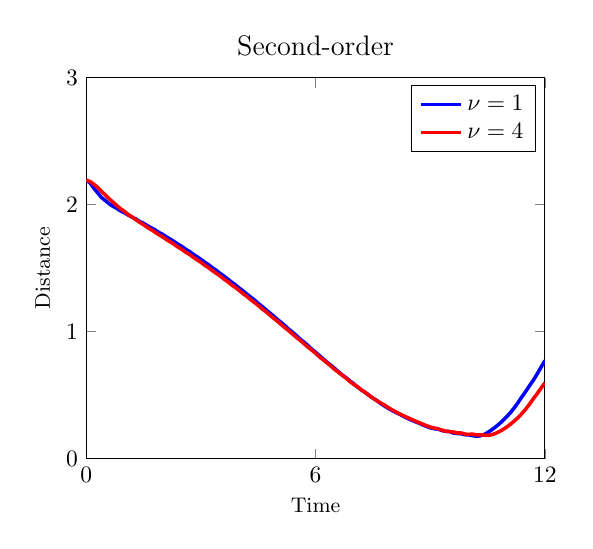
\begin{tikzpicture}[scale=0.85]

\begin{axis}[
  xmin = 0,
  xmax = 12, 
  ymin = 0,
  ymax = 3,
  xtick = {0,6,12,18,24},
  xticklabels = {$0$,$6$,$12$,$18$,$24$},
  ytick = {0,1,2,3},
  yticklabels = {$0$,$1$,$2$,$3$},
  xlabel = {Time},
  ylabel = {Distance},
  label style = {font=\small},
  legend entries = {$\nu=1$,$\nu=4$},
  title = {\large{Second-order}}
  ]

\addplot [mark=none,blue,line width=1.5] table{
0.0000e+00 2.1913e+00
1.0000e-01 2.1712e+00
2.0000e-01 2.1289e+00
3.0000e-01 2.0918e+00
4.0000e-01 2.0561e+00
5.0000e-01 2.0316e+00
6.0000e-01 2.0064e+00
7.0000e-01 1.9862e+00
8.0000e-01 1.9698e+00
9.0000e-01 1.9493e+00
1.0000e+00 1.9355e+00
1.1000e+00 1.9170e+00
1.2000e+00 1.9005e+00
1.3000e+00 1.8861e+00
1.4000e+00 1.8667e+00
1.5000e+00 1.8528e+00
1.6000e+00 1.8338e+00
1.7000e+00 1.8168e+00
1.8000e+00 1.8012e+00
1.9000e+00 1.7807e+00
2.0000e+00 1.7651e+00
2.1000e+00 1.7448e+00
2.2000e+00 1.7275e+00
2.3000e+00 1.7086e+00
2.4000e+00 1.6882e+00
2.5000e+00 1.6707e+00
2.6000e+00 1.6487e+00
2.7000e+00 1.6309e+00
2.8000e+00 1.6088e+00
2.9000e+00 1.5893e+00
3.0000e+00 1.5685e+00
3.1000e+00 1.5462e+00
3.2000e+00 1.5264e+00
3.3000e+00 1.5026e+00
3.4000e+00 1.4826e+00
3.5000e+00 1.4587e+00
3.6000e+00 1.4376e+00
3.7000e+00 1.4143e+00
3.8000e+00 1.3905e+00
3.9000e+00 1.3687e+00
4.0000e+00 1.3431e+00
4.1000e+00 1.3213e+00
4.2000e+00 1.2958e+00
4.3000e+00 1.2723e+00
4.4000e+00 1.2488e+00
4.5000e+00 1.2219e+00
4.6000e+00 1.1989e+00
4.7000e+00 1.1724e+00
4.8000e+00 1.1476e+00
4.9000e+00 1.1232e+00
5.0000e+00 1.0956e+00
5.1000e+00 1.0723e+00
5.2000e+00 1.0466e+00
5.3000e+00 1.0181e+00
5.4000e+00 9.9453e-01
5.5000e+00 9.6845e-01
5.6000e+00 9.3987e-01
5.7000e+00 9.1647e-01
5.8000e+00 8.9028e-01
5.9000e+00 8.6159e-01
6.0000e+00 8.3755e-01
6.1000e+00 8.1164e-01
6.2000e+00 7.8490e-01
6.3000e+00 7.5844e-01
6.4000e+00 7.3551e-01
6.5000e+00 7.0981e-01
6.6000e+00 6.8334e-01
6.7000e+00 6.5805e-01
6.8000e+00 6.3685e-01
6.9000e+00 6.1128e-01
7.0000e+00 5.8893e-01
7.1000e+00 5.6274e-01
7.2000e+00 5.4031e-01
7.3000e+00 5.2142e-01
7.4000e+00 4.9766e-01
7.5000e+00 4.7671e-01
7.6000e+00 4.5791e-01
7.7000e+00 4.3511e-01
7.8000e+00 4.1462e-01
7.9000e+00 3.9613e-01
8.0000e+00 3.7929e-01
8.1000e+00 3.6372e-01
8.2000e+00 3.4906e-01
8.3000e+00 3.3319e-01
8.4000e+00 3.1795e-01
8.5000e+00 3.0410e-01
8.6000e+00 2.9176e-01
8.7000e+00 2.7961e-01
8.8000e+00 2.6613e-01
8.9000e+00 2.5359e-01
9.0000e+00 2.4294e-01
9.1000e+00 2.3543e-01
9.2000e+00 2.3249e-01
9.3000e+00 2.2164e-01
9.4000e+00 2.1454e-01
9.5000e+00 2.1427e-01
9.6000e+00 2.0195e-01
9.7000e+00 1.9752e-01
9.8000e+00 1.9720e-01
9.9000e+00 1.8803e-01
1.0000e+01 1.8718e-01
1.0100e+01 1.8166e-01
1.0200e+01 1.7608e-01
1.0300e+01 1.7868e-01
1.0400e+01 1.8874e-01
1.0500e+01 2.0467e-01
1.0600e+01 2.2458e-01
1.0700e+01 2.4718e-01
1.0800e+01 2.7200e-01
1.0900e+01 2.9919e-01
1.1000e+01 3.2923e-01
1.1100e+01 3.6272e-01
1.1200e+01 4.0023e-01
1.1300e+01 4.4224e-01
1.1400e+01 4.8731e-01
1.1500e+01 5.2966e-01
1.1600e+01 5.7524e-01
1.1700e+01 6.1828e-01
1.1800e+01 6.6763e-01
1.1900e+01 7.2035e-01
1.2000e+01 7.7138e-01
};

\addplot [mark=none,red,line width=1.5] table{
0.0000e+00 2.1913e+00
1.0000e-01 2.1819e+00
2.0000e-01 2.1594e+00
3.0000e-01 2.1353e+00
4.0000e-01 2.1036e+00
5.0000e-01 2.0762e+00
6.0000e-01 2.0449e+00
7.0000e-01 2.0199e+00
8.0000e-01 1.9922e+00
9.0000e-01 1.9673e+00
1.0000e+00 1.9461e+00
1.1000e+00 1.9211e+00
1.2000e+00 1.9028e+00
1.3000e+00 1.8804e+00
1.4000e+00 1.8595e+00
1.5000e+00 1.8419e+00
1.6000e+00 1.8198e+00
1.7000e+00 1.8027e+00
1.8000e+00 1.7828e+00
1.9000e+00 1.7623e+00
2.0000e+00 1.7453e+00
2.1000e+00 1.7237e+00
2.2000e+00 1.7063e+00
2.3000e+00 1.6863e+00
2.4000e+00 1.6654e+00
2.5000e+00 1.6476e+00
2.6000e+00 1.6254e+00
2.7000e+00 1.6075e+00
2.8000e+00 1.5859e+00
2.9000e+00 1.5647e+00
3.0000e+00 1.5457e+00
3.1000e+00 1.5223e+00
3.2000e+00 1.5033e+00
3.3000e+00 1.4802e+00
3.4000e+00 1.4589e+00
3.5000e+00 1.4382e+00
3.6000e+00 1.4137e+00
3.7000e+00 1.3932e+00
3.8000e+00 1.3688e+00
3.9000e+00 1.3472e+00
4.0000e+00 1.3244e+00
4.1000e+00 1.2992e+00
4.2000e+00 1.2775e+00
4.3000e+00 1.2521e+00
4.4000e+00 1.2292e+00
4.5000e+00 1.2060e+00
4.6000e+00 1.1792e+00
4.7000e+00 1.1570e+00
4.8000e+00 1.1312e+00
4.9000e+00 1.1055e+00
5.0000e+00 1.0822e+00
5.1000e+00 1.0557e+00
5.2000e+00 1.0306e+00
5.3000e+00 1.0066e+00
5.4000e+00 9.7975e-01
5.5000e+00 9.5447e-01
5.6000e+00 9.3032e-01
5.7000e+00 9.0393e-01
5.8000e+00 8.7754e-01
5.9000e+00 8.5433e-01
6.0000e+00 8.2957e-01
6.1000e+00 8.0124e-01
6.2000e+00 7.7788e-01
6.3000e+00 7.5319e-01
6.4000e+00 7.2853e-01
6.5000e+00 7.0171e-01
6.6000e+00 6.7955e-01
6.7000e+00 6.5551e-01
6.8000e+00 6.3309e-01
6.9000e+00 6.0681e-01
7.0000e+00 5.8382e-01
7.1000e+00 5.6465e-01
7.2000e+00 5.4086e-01
7.3000e+00 5.2009e-01
7.4000e+00 4.9837e-01
7.5000e+00 4.7591e-01
7.6000e+00 4.5617e-01
7.7000e+00 4.3884e-01
7.8000e+00 4.2160e-01
7.9000e+00 4.0187e-01
8.0000e+00 3.8391e-01
8.1000e+00 3.6741e-01
8.2000e+00 3.5208e-01
8.3000e+00 3.3761e-01
8.4000e+00 3.2375e-01
8.5000e+00 3.1027e-01
8.6000e+00 2.9704e-01
8.7000e+00 2.8403e-01
8.8000e+00 2.7139e-01
8.9000e+00 2.5944e-01
9.0000e+00 2.4880e-01
9.1000e+00 2.4034e-01
9.2000e+00 2.3522e-01
9.3000e+00 2.2566e-01
9.4000e+00 2.1599e-01
9.5000e+00 2.1204e-01
9.6000e+00 2.0989e-01
9.7000e+00 2.0159e-01
9.8000e+00 2.0188e-01
9.9000e+00 1.9399e-01
1.0000e+01 1.9041e-01
1.0100e+01 1.9345e-01
1.0200e+01 1.8618e-01
1.0300e+01 1.8772e-01
1.0400e+01 1.8549e-01
1.0500e+01 1.8281e-01
1.0600e+01 1.8730e-01
1.0700e+01 1.9754e-01
1.0800e+01 2.1199e-01
1.0900e+01 2.2860e-01
1.1000e+01 2.4809e-01
1.1100e+01 2.7155e-01
1.1200e+01 2.9626e-01
1.1300e+01 3.2396e-01
1.1400e+01 3.5516e-01
1.1500e+01 3.9033e-01
1.1600e+01 4.2984e-01
1.1700e+01 4.7280e-01
1.1800e+01 5.1228e-01
1.1900e+01 5.5581e-01
1.2000e+01 5.9544e-01
};

\end{axis}


\end{tikzpicture}


%\fi
%\end{tabular}
%\mcaption{Two vesicles of reduced Area $0.99$ are submerged in a shear
%flow.  The vesicles in the top row have no viscosity contrast and the
%vesicles in the second row have a viscosity contrast of 4.  The bottom
%plots show the distance between the vesicles for both viscosity
%contrasts with first- and second-order time stepping.  Implicit
%vesicle-vesicle interactions are used for all the simulations.  The gap
%sizes of the first- and second-order methods differ by 2.2\% for $\nu=1$
%and by 1.2\% for $\nu=4$.}{f:shear:reducedArea2}
%\end{figure}

\begin{figure}[htp]
\centering
\begin{tabular}{m{1cm}CCCCC}
\ifInputs
$\nu=1$ &
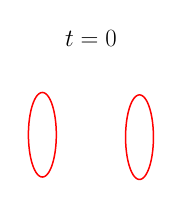
\begin{tikzpicture}[scale=0.36]

\begin{axis}[
  xmin = -6,
  xmax = 2,
  ymin = -2,
  ymax = 2,
  axis equal = true,
  hide axis,
  title = {\Huge$t=0$}
  ]

\addplot [mark=none,red,line width=1.5] table{
-4.0000e+00 1.8412e+00
-4.0563e+00 1.8329e+00
-4.1120e+00 1.8078e+00
-4.1667e+00 1.7663e+00
-4.2198e+00 1.7087e+00
-4.2707e+00 1.6356e+00
-4.3191e+00 1.5478e+00
-4.3643e+00 1.4460e+00
-4.4061e+00 1.3312e+00
-4.4439e+00 1.2046e+00
-4.4775e+00 1.0674e+00
-4.5065e+00 9.2082e-01
-4.5306e+00 7.6635e-01
-4.5496e+00 6.0546e-01
-4.5633e+00 4.3970e-01
-4.5715e+00 2.7067e-01
-4.5743e+00 1.0000e-01
-4.5715e+00 -7.0672e-02
-4.5633e+00 -2.3970e-01
-4.5496e+00 -4.0546e-01
-4.5306e+00 -5.6635e-01
-4.5065e+00 -7.2082e-01
-4.4775e+00 -8.6738e-01
-4.4439e+00 -1.0046e+00
-4.4061e+00 -1.1312e+00
-4.3643e+00 -1.2460e+00
-4.3191e+00 -1.3478e+00
-4.2707e+00 -1.4356e+00
-4.2198e+00 -1.5087e+00
-4.1667e+00 -1.5663e+00
-4.1120e+00 -1.6078e+00
-4.0563e+00 -1.6329e+00
-4.0000e+00 -1.6412e+00
-3.9437e+00 -1.6329e+00
-3.8880e+00 -1.6078e+00
-3.8333e+00 -1.5663e+00
-3.7802e+00 -1.5087e+00
-3.7293e+00 -1.4356e+00
-3.6809e+00 -1.3478e+00
-3.6357e+00 -1.2460e+00
-3.5939e+00 -1.1312e+00
-3.5561e+00 -1.0046e+00
-3.5225e+00 -8.6738e-01
-3.4935e+00 -7.2082e-01
-3.4694e+00 -5.6635e-01
-3.4504e+00 -4.0546e-01
-3.4367e+00 -2.3970e-01
-3.4285e+00 -7.0672e-02
-3.4257e+00 1.0000e-01
-3.4285e+00 2.7067e-01
-3.4367e+00 4.3970e-01
-3.4504e+00 6.0546e-01
-3.4694e+00 7.6635e-01
-3.4935e+00 9.2082e-01
-3.5225e+00 1.0674e+00
-3.5561e+00 1.2046e+00
-3.5939e+00 1.3312e+00
-3.6357e+00 1.4460e+00
-3.6809e+00 1.5478e+00
-3.7293e+00 1.6356e+00
-3.7802e+00 1.7087e+00
-3.8333e+00 1.7663e+00
-3.8880e+00 1.8078e+00
-3.9437e+00 1.8329e+00
-4.0000e+00 1.8412e+00
};

\addplot [mark=none,red,line width=1.5] table{
1.0662e-16 1.7412e+00
-5.6291e-02 1.7329e+00
-1.1204e-01 1.7078e+00
-1.6671e-01 1.6663e+00
-2.1978e-01 1.6087e+00
-2.7072e-01 1.5356e+00
-3.1907e-01 1.4478e+00
-3.6433e-01 1.3460e+00
-4.0609e-01 1.2312e+00
-4.4394e-01 1.1046e+00
-4.7751e-01 9.6738e-01
-5.0649e-01 8.2082e-01
-5.3059e-01 6.6635e-01
-5.4957e-01 5.0546e-01
-5.6327e-01 3.3970e-01
-5.7154e-01 1.7067e-01
-5.7430e-01 1.4179e-16
-5.7154e-01 -1.7067e-01
-5.6327e-01 -3.3970e-01
-5.4957e-01 -5.0546e-01
-5.3059e-01 -6.6635e-01
-5.0649e-01 -8.2082e-01
-4.7751e-01 -9.6738e-01
-4.4394e-01 -1.1046e+00
-4.0609e-01 -1.2312e+00
-3.6433e-01 -1.3460e+00
-3.1907e-01 -1.4478e+00
-2.7072e-01 -1.5356e+00
-2.1978e-01 -1.6087e+00
-1.6671e-01 -1.6663e+00
-1.1204e-01 -1.7078e+00
-5.6291e-02 -1.7329e+00
-1.7695e-16 -1.7412e+00
5.6291e-02 -1.7329e+00
1.1204e-01 -1.7078e+00
1.6671e-01 -1.6663e+00
2.1978e-01 -1.6087e+00
2.7072e-01 -1.5356e+00
3.1907e-01 -1.4478e+00
3.6433e-01 -1.3460e+00
4.0609e-01 -1.2312e+00
4.4394e-01 -1.1046e+00
4.7751e-01 -9.6738e-01
5.0649e-01 -8.2082e-01
5.3059e-01 -6.6635e-01
5.4957e-01 -5.0546e-01
5.6327e-01 -3.3970e-01
5.7154e-01 -1.7067e-01
5.7430e-01 -3.5503e-16
5.7154e-01 1.7067e-01
5.6327e-01 3.3970e-01
5.4957e-01 5.0546e-01
5.3059e-01 6.6635e-01
5.0649e-01 8.2082e-01
4.7751e-01 9.6738e-01
4.4394e-01 1.1046e+00
4.0609e-01 1.2312e+00
3.6433e-01 1.3460e+00
3.1907e-01 1.4478e+00
2.7072e-01 1.5356e+00
2.1978e-01 1.6087e+00
1.6671e-01 1.6663e+00
1.1204e-01 1.7078e+00
5.6291e-02 1.7329e+00
1.0662e-16 1.7412e+00
};

\end{axis}
\end{tikzpicture}

 &
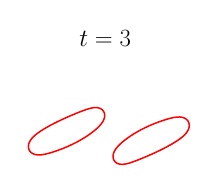
\begin{tikzpicture}[scale=0.36]

\begin{axis}[
  xmin = -6,
  xmax = 2,
  ymin = -2,
  ymax = 2,
  axis equal = true,
  hide axis,
  title = {\Huge$t=3$}
  ]

\addplot [mark=none,red,line width=1.5] table{
-2.0216e+00 8.7489e-01
-2.0233e+00 9.3267e-01
-2.0358e+00 9.9339e-01
-2.0637e+00 1.0570e+00
-2.1121e+00 1.1195e+00
-2.1842e+00 1.1728e+00
-2.2785e+00 1.2082e+00
-2.3897e+00 1.2204e+00
-2.5119e+00 1.2099e+00
-2.6416e+00 1.1811e+00
-2.7773e+00 1.1393e+00
-2.9189e+00 1.0888e+00
-3.0657e+00 1.0324e+00
-3.2171e+00 9.7161e-01
-3.3716e+00 9.0723e-01
-3.5281e+00 8.3970e-01
-3.6850e+00 7.6943e-01
-3.8409e+00 6.9686e-01
-3.9943e+00 6.2249e-01
-4.1438e+00 5.4682e-01
-4.2881e+00 4.7036e-01
-4.4256e+00 3.9354e-01
-4.5551e+00 3.1667e-01
-4.6751e+00 2.3994e-01
-4.7840e+00 1.6343e-01
-4.8804e+00 8.7178e-02
-4.9629e+00 1.1381e-02
-5.0307e+00 -6.3431e-02
-5.0831e+00 -1.3627e-01
-5.1209e+00 -2.0583e-01
-5.1454e+00 -2.7103e-01
-5.1585e+00 -3.3175e-01
-5.1622e+00 -3.8945e-01
-5.1565e+00 -4.4690e-01
-5.1396e+00 -5.0645e-01
-5.1074e+00 -5.6793e-01
-5.0556e+00 -6.2757e-01
-4.9820e+00 -6.7874e-01
-4.8877e+00 -7.1452e-01
-4.7770e+00 -7.3097e-01
-4.6543e+00 -7.2834e-01
-4.5227e+00 -7.0970e-01
-4.3840e+00 -6.7883e-01
-4.2391e+00 -6.3882e-01
-4.0890e+00 -5.9162e-01
-3.9349e+00 -5.3831e-01
-3.7781e+00 -4.7944e-01
-3.6202e+00 -4.1536e-01
-3.4628e+00 -3.4636e-01
-3.3075e+00 -2.7281e-01
-3.1557e+00 -1.9520e-01
-3.0092e+00 -1.1412e-01
-2.8691e+00 -3.0388e-02
-2.7368e+00 5.5055e-02
-2.6133e+00 1.4115e-01
-2.4997e+00 2.2684e-01
-2.3968e+00 3.1123e-01
-2.3056e+00 3.9362e-01
-2.2270e+00 4.7350e-01
-2.1618e+00 5.5041e-01
-2.1100e+00 6.2377e-01
-2.0715e+00 6.9292e-01
-2.0449e+00 7.5736e-01
-2.0288e+00 8.1744e-01
-2.0216e+00 8.7489e-01
};

\addplot [mark=none,red,line width=1.5] table{
1.4622e+00 4.8945e-01
1.4565e+00 5.4690e-01
1.4396e+00 6.0645e-01
1.4074e+00 6.6793e-01
1.3556e+00 7.2757e-01
1.2820e+00 7.7874e-01
1.1877e+00 8.1452e-01
1.0770e+00 8.3097e-01
9.5426e-01 8.2834e-01
8.2270e-01 8.0970e-01
6.8398e-01 7.7883e-01
5.3908e-01 7.3882e-01
3.8899e-01 6.9162e-01
2.3487e-01 6.3831e-01
7.8119e-02 5.7944e-01
-7.9760e-02 5.1536e-01
-2.3718e-01 4.4636e-01
-3.9253e-01 3.7281e-01
-5.4425e-01 2.9520e-01
-6.9083e-01 2.1412e-01
-8.3089e-01 1.3039e-01
-9.6319e-01 4.4945e-02
-1.0867e+00 -4.1147e-02
-1.2003e+00 -1.2684e-01
-1.3032e+00 -2.1123e-01
-1.3944e+00 -2.9362e-01
-1.4730e+00 -3.7350e-01
-1.5382e+00 -4.5041e-01
-1.5900e+00 -5.2377e-01
-1.6285e+00 -5.9292e-01
-1.6551e+00 -6.5736e-01
-1.6712e+00 -7.1744e-01
-1.6784e+00 -7.7489e-01
-1.6767e+00 -8.3267e-01
-1.6642e+00 -8.9339e-01
-1.6363e+00 -9.5703e-01
-1.5879e+00 -1.0195e+00
-1.5158e+00 -1.0728e+00
-1.4215e+00 -1.1082e+00
-1.3103e+00 -1.1204e+00
-1.1881e+00 -1.1099e+00
-1.0584e+00 -1.0811e+00
-9.2265e-01 -1.0393e+00
-7.8111e-01 -9.8879e-01
-6.3425e-01 -9.3239e-01
-4.8294e-01 -8.7161e-01
-3.2837e-01 -8.0723e-01
-1.7190e-01 -7.3970e-01
-1.5005e-02 -6.6943e-01
1.4087e-01 -5.9686e-01
2.9428e-01 -5.2249e-01
4.4381e-01 -4.4682e-01
5.8806e-01 -3.7036e-01
7.2564e-01 -2.9354e-01
8.5513e-01 -2.1667e-01
9.7508e-01 -1.3994e-01
1.0840e+00 -6.3428e-02
1.1804e+00 1.2822e-02
1.2629e+00 8.8619e-02
1.3307e+00 1.6343e-01
1.3831e+00 2.3627e-01
1.4209e+00 3.0583e-01
1.4454e+00 3.7103e-01
1.4585e+00 4.3175e-01
1.4622e+00 4.8945e-01
};

\end{axis}
\end{tikzpicture}

 &
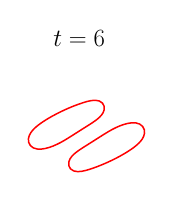
\begin{tikzpicture}[scale=0.36]

\begin{axis}[
  xmin = -6,
  xmax = 2,
  ymin = -2,
  ymax = 2,
  axis equal = true,
  hide axis,
  title = {\Huge$t=6$}
  ]

\addplot [mark=none,red,line width=1.5] table{
-1.5410e+00 5.4046e-01
-1.4923e+00 5.7219e-01
-1.4402e+00 6.0678e-01
-1.3823e+00 6.4647e-01
-1.3172e+00 6.9321e-01
-1.2451e+00 7.4900e-01
-1.1676e+00 8.1643e-01
-1.0891e+00 8.9908e-01
-1.0179e+00 1.0017e+00
-9.7044e-01 1.1277e+00
-9.7153e-01 1.2707e+00
-1.0418e+00 1.4034e+00
-1.1725e+00 1.4898e+00
-1.3324e+00 1.5193e+00
-1.4993e+00 1.5070e+00
-1.6658e+00 1.4711e+00
-1.8309e+00 1.4230e+00
-1.9938e+00 1.3681e+00
-2.1538e+00 1.3092e+00
-2.3097e+00 1.2476e+00
-2.4601e+00 1.1842e+00
-2.6040e+00 1.1199e+00
-2.7403e+00 1.0558e+00
-2.8679e+00 9.9261e-01
-2.9861e+00 9.3139e-01
-3.0943e+00 8.7295e-01
-3.1920e+00 8.1798e-01
-3.2793e+00 7.6701e-01
-3.3561e+00 7.2039e-01
-3.4233e+00 6.7817e-01
-3.4818e+00 6.4007e-01
-3.5336e+00 6.0522e-01
-3.5813e+00 5.7199e-01
-3.6284e+00 5.3794e-01
-3.6782e+00 5.0032e-01
-3.7331e+00 4.5661e-01
-3.7939e+00 4.0460e-01
-3.8601e+00 3.4210e-01
-3.9295e+00 2.6669e-01
-3.9975e+00 1.7547e-01
-4.0558e+00 6.5359e-02
-4.0903e+00 -6.4585e-02
-4.0815e+00 -2.0741e-01
-4.0137e+00 -3.4173e-01
-3.8907e+00 -4.3937e-01
-3.7351e+00 -4.8701e-01
-3.5680e+00 -4.9161e-01
-3.3995e+00 -4.6660e-01
-3.2335e+00 -4.2208e-01
-3.0718e+00 -3.6385e-01
-2.9158e+00 -2.9542e-01
-2.7663e+00 -2.1982e-01
-2.6239e+00 -1.4009e-01
-2.4888e+00 -5.9196e-02
-2.3610e+00 2.0337e-02
-2.2407e+00 9.6581e-02
-2.1285e+00 1.6817e-01
-2.0249e+00 2.3421e-01
-1.9302e+00 2.9425e-01
-1.8449e+00 3.4813e-01
-1.7688e+00 3.9601e-01
-1.7017e+00 4.3826e-01
-1.6426e+00 4.7556e-01
-1.5899e+00 5.0904e-01
-1.5410e+00 5.4046e-01
};

\addplot [mark=none,red,line width=1.5] table{
1.8128e-01 -4.7199e-01
2.2837e-01 -4.3794e-01
2.7821e-01 -4.0032e-01
3.3307e-01 -3.5661e-01
3.9388e-01 -3.0460e-01
4.6009e-01 -2.4210e-01
5.2951e-01 -1.6669e-01
5.9754e-01 -7.5465e-02
6.5584e-01 3.4641e-02
6.9030e-01 1.6458e-01
6.8152e-01 3.0741e-01
6.1369e-01 4.4173e-01
4.9073e-01 5.3937e-01
3.3515e-01 5.8701e-01
1.6796e-01 5.9161e-01
-4.8922e-04 5.6660e-01
-1.6646e-01 5.2208e-01
-3.2815e-01 4.6385e-01
-4.8423e-01 3.9542e-01
-6.3370e-01 3.1982e-01
-7.7608e-01 2.4009e-01
-9.1123e-01 1.5920e-01
-1.0390e+00 7.9663e-02
-1.1593e+00 3.4189e-03
-1.2715e+00 -6.8167e-02
-1.3751e+00 -1.3421e-01
-1.4698e+00 -1.9425e-01
-1.5551e+00 -2.4813e-01
-1.6312e+00 -2.9601e-01
-1.6983e+00 -3.3826e-01
-1.7574e+00 -3.7556e-01
-1.8101e+00 -4.0904e-01
-1.8590e+00 -4.4046e-01
-1.9077e+00 -4.7219e-01
-1.9598e+00 -5.0678e-01
-2.0177e+00 -5.4647e-01
-2.0828e+00 -5.9321e-01
-2.1549e+00 -6.4900e-01
-2.2324e+00 -7.1643e-01
-2.3109e+00 -7.9908e-01
-2.3821e+00 -9.0168e-01
-2.4296e+00 -1.0277e+00
-2.4285e+00 -1.1707e+00
-2.3582e+00 -1.3034e+00
-2.2275e+00 -1.3898e+00
-2.0676e+00 -1.4193e+00
-1.9007e+00 -1.4070e+00
-1.7342e+00 -1.3711e+00
-1.5691e+00 -1.3230e+00
-1.4062e+00 -1.2681e+00
-1.2462e+00 -1.2092e+00
-1.0903e+00 -1.1476e+00
-9.3986e-01 -1.0842e+00
-7.9598e-01 -1.0199e+00
-6.5973e-01 -9.5576e-01
-5.3209e-01 -8.9261e-01
-4.1387e-01 -8.3139e-01
-3.0569e-01 -7.7295e-01
-2.0795e-01 -7.1798e-01
-1.2075e-01 -6.6701e-01
-4.3859e-02 -6.2039e-01
2.3301e-02 -5.7817e-01
8.1850e-02 -5.4007e-01
1.3359e-01 -5.0522e-01
1.8128e-01 -4.7199e-01
};

\end{axis}
\end{tikzpicture}

 &
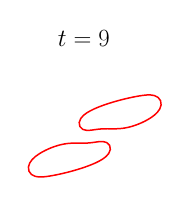
\begin{tikzpicture}[scale=0.36]

\begin{axis}[
  xmin = -6,
  xmax = 2,
  ymin = -2,
  ymax = 2,
  axis equal = true,
  hide axis,
  title = {\Huge$t=9$}
  ]

\addplot [mark=none,red,line width=1.5] table{
-4.3957e-01 3.6041e-01
-3.8178e-01 3.6751e-01
-3.1988e-01 3.7671e-01
-2.5066e-01 3.8903e-01
-1.7215e-01 4.0552e-01
-8.3497e-02 4.2740e-01
1.5384e-02 4.5571e-01
1.2394e-01 4.9146e-01
2.4132e-01 5.3538e-01
3.6627e-01 5.8815e-01
4.9734e-01 6.5032e-01
6.3253e-01 7.2278e-01
7.6930e-01 8.0693e-01
9.0353e-01 9.0552e-01
1.0280e+00 1.0229e+00
1.1288e+00 1.1646e+00
1.1818e+00 1.3307e+00
1.1588e+00 1.5019e+00
1.0562e+00 1.6376e+00
9.0703e-01 1.7131e+00
7.4599e-01 1.7389e+00
5.8841e-01 1.7366e+00
4.3855e-01 1.7211e+00
2.9763e-01 1.7002e+00
1.6642e-01 1.6772e+00
4.5633e-02 1.6539e+00
-6.4224e-02 1.6311e+00
-1.6293e-01 1.6094e+00
-2.5060e-01 1.5892e+00
-3.2778e-01 1.5707e+00
-3.9562e-01 1.5539e+00
-4.5611e-01 1.5385e+00
-5.1237e-01 1.5238e+00
-5.6854e-01 1.5087e+00
-6.2880e-01 1.4922e+00
-6.9637e-01 1.4731e+00
-7.7328e-01 1.4508e+00
-8.6058e-01 1.4246e+00
-9.5856e-01 1.3941e+00
-1.0670e+00 1.3587e+00
-1.1852e+00 1.3181e+00
-1.3122e+00 1.2715e+00
-1.4469e+00 1.2183e+00
-1.5873e+00 1.1572e+00
-1.7314e+00 1.0864e+00
-1.8751e+00 1.0023e+00
-2.0118e+00 8.9956e-01
-2.1269e+00 7.6930e-01
-2.1908e+00 6.0729e-01
-2.1627e+00 4.3764e-01
-2.0411e+00 3.1999e-01
-1.8791e+00 2.7936e-01
-1.7161e+00 2.8575e-01
-1.5599e+00 3.0741e-01
-1.4106e+00 3.2740e-01
-1.2687e+00 3.4022e-01
-1.1355e+00 3.4571e-01
-1.0125e+00 3.4645e-01
-9.0021e-01 3.4522e-01
-7.9912e-01 3.4426e-01
-7.0911e-01 3.4463e-01
-6.2971e-01 3.4665e-01
-5.5984e-01 3.5010e-01
-4.9752e-01 3.5472e-01
-4.3957e-01 3.6041e-01
};

\addplot [mark=none,red,line width=1.5] table{
-2.5876e+00 -1.4238e+00
-2.5315e+00 -1.4087e+00
-2.4712e+00 -1.3922e+00
-2.4036e+00 -1.3731e+00
-2.3267e+00 -1.3508e+00
-2.2394e+00 -1.3246e+00
-2.1414e+00 -1.2941e+00
-2.0330e+00 -1.2587e+00
-1.9148e+00 -1.2181e+00
-1.7878e+00 -1.1715e+00
-1.6531e+00 -1.1183e+00
-1.5127e+00 -1.0572e+00
-1.3686e+00 -9.8637e-01
-1.2249e+00 -9.0234e-01
-1.0882e+00 -7.9956e-01
-9.7311e-01 -6.6930e-01
-9.0918e-01 -5.0729e-01
-9.3734e-01 -3.3764e-01
-1.0589e+00 -2.1999e-01
-1.2209e+00 -1.7936e-01
-1.3839e+00 -1.8575e-01
-1.5401e+00 -2.0741e-01
-1.6894e+00 -2.2740e-01
-1.8313e+00 -2.4022e-01
-1.9645e+00 -2.4571e-01
-2.0875e+00 -2.4645e-01
-2.1998e+00 -2.4522e-01
-2.3009e+00 -2.4426e-01
-2.3909e+00 -2.4463e-01
-2.4703e+00 -2.4665e-01
-2.5402e+00 -2.5010e-01
-2.6025e+00 -2.5472e-01
-2.6604e+00 -2.6041e-01
-2.7182e+00 -2.6751e-01
-2.7801e+00 -2.7671e-01
-2.8493e+00 -2.8903e-01
-2.9279e+00 -3.0552e-01
-3.0165e+00 -3.2740e-01
-3.1154e+00 -3.5571e-01
-3.2239e+00 -3.9146e-01
-3.3413e+00 -4.3538e-01
-3.4663e+00 -4.8815e-01
-3.5973e+00 -5.5032e-01
-3.7325e+00 -6.2278e-01
-3.8693e+00 -7.0693e-01
-4.0035e+00 -8.0552e-01
-4.1280e+00 -9.2295e-01
-4.2288e+00 -1.0646e+00
-4.2818e+00 -1.2307e+00
-4.2588e+00 -1.4019e+00
-4.1562e+00 -1.5376e+00
-4.0070e+00 -1.6131e+00
-3.8460e+00 -1.6389e+00
-3.6884e+00 -1.6366e+00
-3.5386e+00 -1.6211e+00
-3.3976e+00 -1.6002e+00
-3.2664e+00 -1.5772e+00
-3.1456e+00 -1.5539e+00
-3.0358e+00 -1.5311e+00
-2.9371e+00 -1.5094e+00
-2.8494e+00 -1.4892e+00
-2.7722e+00 -1.4707e+00
-2.7044e+00 -1.4539e+00
-2.6439e+00 -1.4385e+00
-2.5876e+00 -1.4238e+00
};

\end{axis}
\end{tikzpicture}

 &
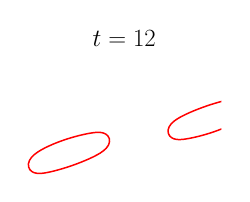
\begin{tikzpicture}[scale=0.36]

\begin{axis}[
  xmin = -6,
  xmax = 2,
  ymin = -2,
  ymax = 2,
  axis equal = true,
  hide axis,
  title = {\Huge$t=12$}
  ]

\addplot [mark=none,red,line width=1.5] table{
4.0724e-01 -9.1055e-02
4.6516e-01 -8.4515e-02
5.2711e-01 -7.5991e-02
5.9659e-01 -6.4890e-02
6.7552e-01 -5.0781e-02
7.6518e-01 -3.3150e-02
8.6573e-01 -1.1733e-02
9.7719e-01 1.3863e-02
1.0988e+00 4.3860e-02
1.2300e+00 7.8635e-02
1.3695e+00 1.1836e-01
1.5162e+00 1.6330e-01
1.6688e+00 2.1349e-01
1.8260e+00 2.6903e-01
1.9862e+00 3.2984e-01
2.1479e+00 3.9590e-01
2.3089e+00 4.6710e-01
2.4676e+00 5.4375e-01
2.6213e+00 6.2646e-01
2.7672e+00 7.1672e-01
2.9008e+00 8.1675e-01
3.0157e+00 9.2954e-01
3.1013e+00 1.0567e+00
3.1451e+00 1.1943e+00
3.1376e+00 1.3284e+00
3.0837e+00 1.4395e+00
3.0016e+00 1.5162e+00
2.9111e+00 1.5613e+00
2.8238e+00 1.5837e+00
2.7449e+00 1.5924e+00
2.6750e+00 1.5934e+00
2.6127e+00 1.5903e+00
2.5547e+00 1.5847e+00
2.4971e+00 1.5772e+00
2.4353e+00 1.5674e+00
2.3663e+00 1.5547e+00
2.2878e+00 1.5386e+00
2.1989e+00 1.5187e+00
2.0991e+00 1.4946e+00
1.9888e+00 1.4661e+00
1.8682e+00 1.4330e+00
1.7383e+00 1.3952e+00
1.5999e+00 1.3525e+00
1.4543e+00 1.3050e+00
1.3025e+00 1.2525e+00
1.1460e+00 1.1955e+00
9.8599e-01 1.1339e+00
8.2420e-01 1.0681e+00
6.6208e-01 9.9817e-01
5.0178e-01 9.2403e-01
3.4527e-01 8.4480e-01
1.9568e-01 7.5876e-01
5.7673e-02 6.6303e-01
-6.1168e-02 5.5398e-01
-1.5005e-01 4.2875e-01
-1.9434e-01 2.9128e-01
-1.8435e-01 1.5733e-01
-1.2647e-01 4.8230e-02
-4.1697e-02 -2.5554e-02
5.0197e-02 -6.7980e-02
1.3773e-01 -8.8984e-02
2.1681e-01 -9.7173e-02
2.8673e-01 -9.8374e-02
3.4924e-01 -9.5786e-02
4.0724e-01 -9.1055e-02
};

\addplot [mark=none,red,line width=1.5] table{
-5.3547e+00 -1.4847e+00
-5.2971e+00 -1.4772e+00
-5.2353e+00 -1.4674e+00
-5.1663e+00 -1.4547e+00
-5.0878e+00 -1.4386e+00
-4.9989e+00 -1.4187e+00
-4.8991e+00 -1.3946e+00
-4.7888e+00 -1.3661e+00
-4.6682e+00 -1.3330e+00
-4.5383e+00 -1.2952e+00
-4.3999e+00 -1.2525e+00
-4.2543e+00 -1.2050e+00
-4.1025e+00 -1.1525e+00
-3.9460e+00 -1.0955e+00
-3.7860e+00 -1.0339e+00
-3.6242e+00 -9.6810e-01
-3.4621e+00 -8.9817e-01
-3.3018e+00 -8.2403e-01
-3.1453e+00 -7.4480e-01
-2.9957e+00 -6.5876e-01
-2.8577e+00 -5.6303e-01
-2.7388e+00 -4.5398e-01
-2.6499e+00 -3.2875e-01
-2.6057e+00 -1.9128e-01
-2.6156e+00 -5.7335e-02
-2.6735e+00 5.1770e-02
-2.7583e+00 1.2555e-01
-2.8502e+00 1.6798e-01
-2.9377e+00 1.8898e-01
-3.0168e+00 1.9717e-01
-3.0867e+00 1.9837e-01
-3.1492e+00 1.9579e-01
-3.2072e+00 1.9105e-01
-3.2652e+00 1.8451e-01
-3.3271e+00 1.7599e-01
-3.3966e+00 1.6489e-01
-3.4755e+00 1.5078e-01
-3.5652e+00 1.3315e-01
-3.6657e+00 1.1173e-01
-3.7772e+00 8.6137e-02
-3.8988e+00 5.6140e-02
-4.0300e+00 2.1365e-02
-4.1695e+00 -1.8363e-02
-4.3162e+00 -6.3304e-02
-4.4688e+00 -1.1349e-01
-4.6260e+00 -1.6903e-01
-4.7862e+00 -2.2984e-01
-4.9479e+00 -2.9590e-01
-5.1089e+00 -3.6710e-01
-5.2676e+00 -4.4375e-01
-5.4213e+00 -5.2646e-01
-5.5672e+00 -6.1672e-01
-5.7008e+00 -7.1675e-01
-5.8157e+00 -8.2954e-01
-5.9013e+00 -9.5669e-01
-5.9451e+00 -1.0943e+00
-5.9376e+00 -1.2284e+00
-5.8837e+00 -1.3395e+00
-5.8016e+00 -1.4162e+00
-5.7111e+00 -1.4613e+00
-5.6238e+00 -1.4837e+00
-5.5449e+00 -1.4924e+00
-5.4750e+00 -1.4934e+00
-5.4127e+00 -1.4903e+00
-5.3547e+00 -1.4847e+00
};

\end{axis}
\end{tikzpicture}

 \\
$\nu=4$ &
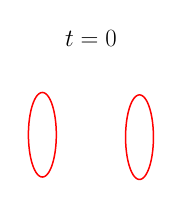
\begin{tikzpicture}[scale=0.36]

\begin{axis}[
  xmin = -6,
  xmax = 2,
  ymin = -2,
  ymax = 2,
  axis equal = true,
  hide axis,
  title = {\Huge$t=0$}
  ]

\addplot [mark=none,red,line width=1.5] table{
-4.0000e+00 1.8412e+00
-4.0563e+00 1.8329e+00
-4.1120e+00 1.8078e+00
-4.1667e+00 1.7663e+00
-4.2198e+00 1.7087e+00
-4.2707e+00 1.6356e+00
-4.3191e+00 1.5478e+00
-4.3643e+00 1.4460e+00
-4.4061e+00 1.3312e+00
-4.4439e+00 1.2046e+00
-4.4775e+00 1.0674e+00
-4.5065e+00 9.2082e-01
-4.5306e+00 7.6635e-01
-4.5496e+00 6.0546e-01
-4.5633e+00 4.3970e-01
-4.5715e+00 2.7067e-01
-4.5743e+00 1.0000e-01
-4.5715e+00 -7.0672e-02
-4.5633e+00 -2.3970e-01
-4.5496e+00 -4.0546e-01
-4.5306e+00 -5.6635e-01
-4.5065e+00 -7.2082e-01
-4.4775e+00 -8.6738e-01
-4.4439e+00 -1.0046e+00
-4.4061e+00 -1.1312e+00
-4.3643e+00 -1.2460e+00
-4.3191e+00 -1.3478e+00
-4.2707e+00 -1.4356e+00
-4.2198e+00 -1.5087e+00
-4.1667e+00 -1.5663e+00
-4.1120e+00 -1.6078e+00
-4.0563e+00 -1.6329e+00
-4.0000e+00 -1.6412e+00
-3.9437e+00 -1.6329e+00
-3.8880e+00 -1.6078e+00
-3.8333e+00 -1.5663e+00
-3.7802e+00 -1.5087e+00
-3.7293e+00 -1.4356e+00
-3.6809e+00 -1.3478e+00
-3.6357e+00 -1.2460e+00
-3.5939e+00 -1.1312e+00
-3.5561e+00 -1.0046e+00
-3.5225e+00 -8.6738e-01
-3.4935e+00 -7.2082e-01
-3.4694e+00 -5.6635e-01
-3.4504e+00 -4.0546e-01
-3.4367e+00 -2.3970e-01
-3.4285e+00 -7.0672e-02
-3.4257e+00 1.0000e-01
-3.4285e+00 2.7067e-01
-3.4367e+00 4.3970e-01
-3.4504e+00 6.0546e-01
-3.4694e+00 7.6635e-01
-3.4935e+00 9.2082e-01
-3.5225e+00 1.0674e+00
-3.5561e+00 1.2046e+00
-3.5939e+00 1.3312e+00
-3.6357e+00 1.4460e+00
-3.6809e+00 1.5478e+00
-3.7293e+00 1.6356e+00
-3.7802e+00 1.7087e+00
-3.8333e+00 1.7663e+00
-3.8880e+00 1.8078e+00
-3.9437e+00 1.8329e+00
-4.0000e+00 1.8412e+00
};

\addplot [mark=none,red,line width=1.5] table{
1.0662e-16 1.7412e+00
-5.6291e-02 1.7329e+00
-1.1204e-01 1.7078e+00
-1.6671e-01 1.6663e+00
-2.1978e-01 1.6087e+00
-2.7072e-01 1.5356e+00
-3.1907e-01 1.4478e+00
-3.6433e-01 1.3460e+00
-4.0609e-01 1.2312e+00
-4.4394e-01 1.1046e+00
-4.7751e-01 9.6738e-01
-5.0649e-01 8.2082e-01
-5.3059e-01 6.6635e-01
-5.4957e-01 5.0546e-01
-5.6327e-01 3.3970e-01
-5.7154e-01 1.7067e-01
-5.7430e-01 1.4179e-16
-5.7154e-01 -1.7067e-01
-5.6327e-01 -3.3970e-01
-5.4957e-01 -5.0546e-01
-5.3059e-01 -6.6635e-01
-5.0649e-01 -8.2082e-01
-4.7751e-01 -9.6738e-01
-4.4394e-01 -1.1046e+00
-4.0609e-01 -1.2312e+00
-3.6433e-01 -1.3460e+00
-3.1907e-01 -1.4478e+00
-2.7072e-01 -1.5356e+00
-2.1978e-01 -1.6087e+00
-1.6671e-01 -1.6663e+00
-1.1204e-01 -1.7078e+00
-5.6291e-02 -1.7329e+00
-1.7695e-16 -1.7412e+00
5.6291e-02 -1.7329e+00
1.1204e-01 -1.7078e+00
1.6671e-01 -1.6663e+00
2.1978e-01 -1.6087e+00
2.7072e-01 -1.5356e+00
3.1907e-01 -1.4478e+00
3.6433e-01 -1.3460e+00
4.0609e-01 -1.2312e+00
4.4394e-01 -1.1046e+00
4.7751e-01 -9.6738e-01
5.0649e-01 -8.2082e-01
5.3059e-01 -6.6635e-01
5.4957e-01 -5.0546e-01
5.6327e-01 -3.3970e-01
5.7154e-01 -1.7067e-01
5.7430e-01 -3.5503e-16
5.7154e-01 1.7067e-01
5.6327e-01 3.3970e-01
5.4957e-01 5.0546e-01
5.3059e-01 6.6635e-01
5.0649e-01 8.2082e-01
4.7751e-01 9.6738e-01
4.4394e-01 1.1046e+00
4.0609e-01 1.2312e+00
3.6433e-01 1.3460e+00
3.1907e-01 1.4478e+00
2.7072e-01 1.5356e+00
2.1978e-01 1.6087e+00
1.6671e-01 1.6663e+00
1.1204e-01 1.7078e+00
5.6291e-02 1.7329e+00
1.0662e-16 1.7412e+00
};

\end{axis}
\end{tikzpicture}

 &
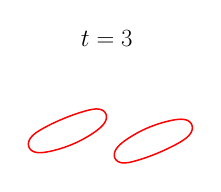
\begin{tikzpicture}[scale=0.36]

\begin{axis}[
  xmin = -6,
  xmax = 2,
  ymin = -2,
  ymax = 2,
  axis equal = true,
  hide axis,
  title = {\Huge$t=3$}
  ]

\addplot [mark=none,red,line width=1.5] table{
-2.0156e+00 8.9140e-01
-2.0309e+00 9.4675e-01
-2.0587e+00 1.0019e+00
-2.1023e+00 1.0555e+00
-2.1649e+00 1.1033e+00
-2.2469e+00 1.1394e+00
-2.3457e+00 1.1590e+00
-2.4576e+00 1.1610e+00
-2.5796e+00 1.1473e+00
-2.7099e+00 1.1215e+00
-2.8477e+00 1.0869e+00
-2.9922e+00 1.0456e+00
-3.1425e+00 9.9896e-01
-3.2972e+00 9.4748e-01
-3.4550e+00 8.9145e-01
-3.6143e+00 8.3116e-01
-3.7737e+00 7.6703e-01
-3.9318e+00 6.9967e-01
-4.0873e+00 6.2985e-01
-4.2388e+00 5.5845e-01
-4.3851e+00 4.8630e-01
-4.5250e+00 4.1402e-01
-4.6571e+00 3.4186e-01
-4.7797e+00 2.6955e-01
-4.8910e+00 1.9646e-01
-4.9887e+00 1.2185e-01
-5.0707e+00 4.5480e-02
-5.1353e+00 -3.1905e-02
-5.1816e+00 -1.0844e-01
-5.2104e+00 -1.8159e-01
-5.2239e+00 -2.4925e-01
-5.2250e+00 -3.1077e-01
-5.2159e+00 -3.6742e-01
-5.1969e+00 -4.2158e-01
-5.1659e+00 -4.7488e-01
-5.1198e+00 -5.2646e-01
-5.0561e+00 -5.7276e-01
-4.9741e+00 -6.0902e-01
-4.8759e+00 -6.3153e-01
-4.7641e+00 -6.3921e-01
-4.6415e+00 -6.3339e-01
-4.5096e+00 -6.1654e-01
-4.3698e+00 -5.9100e-01
-4.2231e+00 -5.5833e-01
-4.0706e+00 -5.1929e-01
-3.9139e+00 -4.7410e-01
-3.7545e+00 -4.2279e-01
-3.5941e+00 -3.6541e-01
-3.4344e+00 -3.0219e-01
-3.2768e+00 -2.3357e-01
-3.1231e+00 -1.6024e-01
-2.9745e+00 -8.3146e-02
-2.8322e+00 -3.4254e-03
-2.6973e+00 7.7735e-02
-2.5709e+00 1.5927e-01
-2.4540e+00 2.4044e-01
-2.3481e+00 3.2093e-01
-2.2545e+00 4.0074e-01
-2.1751e+00 4.7988e-01
-2.1114e+00 5.5795e-01
-2.0640e+00 6.3385e-01
-2.0326e+00 7.0596e-01
-2.0155e+00 7.7286e-01
-2.0105e+00 8.3423e-01
-2.0156e+00 8.9140e-01
};

\addplot [mark=none,red,line width=1.5] table{
1.5159e+00 4.6742e-01
1.4969e+00 5.2158e-01
1.4659e+00 5.7488e-01
1.4198e+00 6.2646e-01
1.3561e+00 6.7276e-01
1.2741e+00 7.0902e-01
1.1759e+00 7.3153e-01
1.0641e+00 7.3921e-01
9.4149e-01 7.3339e-01
8.0965e-01 7.1654e-01
6.6981e-01 6.9100e-01
5.2305e-01 6.5833e-01
3.7062e-01 6.1929e-01
2.1393e-01 5.7410e-01
5.4550e-02 5.2279e-01
-1.0586e-01 4.6541e-01
-2.6564e-01 4.0219e-01
-4.2317e-01 3.3357e-01
-5.7692e-01 2.6024e-01
-7.2554e-01 1.8315e-01
-8.6781e-01 1.0343e-01
-1.0027e+00 2.2265e-02
-1.1291e+00 -5.9272e-02
-1.2460e+00 -1.4044e-01
-1.3519e+00 -2.2093e-01
-1.4455e+00 -3.0074e-01
-1.5249e+00 -3.7988e-01
-1.5886e+00 -4.5795e-01
-1.6360e+00 -5.3385e-01
-1.6674e+00 -6.0596e-01
-1.6845e+00 -6.7286e-01
-1.6895e+00 -7.3423e-01
-1.6844e+00 -7.9140e-01
-1.6691e+00 -8.4675e-01
-1.6413e+00 -9.0185e-01
-1.5977e+00 -9.5551e-01
-1.5351e+00 -1.0033e+00
-1.4531e+00 -1.0394e+00
-1.3543e+00 -1.0590e+00
-1.2424e+00 -1.0610e+00
-1.1204e+00 -1.0473e+00
-9.9009e-01 -1.0215e+00
-8.5228e-01 -9.8688e-01
-7.0775e-01 -9.4561e-01
-5.5751e-01 -8.9896e-01
-4.0280e-01 -8.4748e-01
-2.4503e-01 -7.9145e-01
-8.5698e-02 -7.3116e-01
7.3733e-02 -6.6703e-01
2.3184e-01 -5.9967e-01
3.8727e-01 -5.2985e-01
5.3877e-01 -4.5845e-01
6.8509e-01 -3.8630e-01
8.2500e-01 -3.1402e-01
9.5707e-01 -2.4186e-01
1.0797e+00 -1.6955e-01
1.1910e+00 -9.6456e-02
1.2887e+00 -2.1847e-02
1.3707e+00 5.4520e-02
1.4353e+00 1.3191e-01
1.4816e+00 2.0844e-01
1.5104e+00 2.8159e-01
1.5239e+00 3.4925e-01
1.5250e+00 4.1077e-01
1.5159e+00 4.6742e-01
};

\end{axis}
\end{tikzpicture}

 &
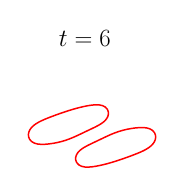
\begin{tikzpicture}[scale=0.36]

\begin{axis}[
  xmin = -6,
  xmax = 2,
  ymin = -2,
  ymax = 2,
  axis equal = true,
  hide axis,
  title = {\Huge$t=6$}
  ]

\addplot [mark=none,red,line width=1.5] table{
-1.2106e+00 6.3920e-01
-1.1683e+00 6.7850e-01
-1.1266e+00 7.2449e-01
-1.0860e+00 7.8110e-01
-1.0501e+00 8.5192e-01
-1.0270e+00 9.3903e-01
-1.0288e+00 1.0401e+00
-1.0680e+00 1.1450e+00
-1.1497e+00 1.2363e+00
-1.2667e+00 1.2987e+00
-1.4053e+00 1.3287e+00
-1.5555e+00 1.3328e+00
-1.7122e+00 1.3194e+00
-1.8734e+00 1.2947e+00
-2.0376e+00 1.2621e+00
-2.2036e+00 1.2236e+00
-2.3698e+00 1.1800e+00
-2.5350e+00 1.1324e+00
-2.6977e+00 1.0818e+00
-2.8568e+00 1.0294e+00
-3.0111e+00 9.7626e-01
-3.1594e+00 9.2348e-01
-3.3008e+00 8.7172e-01
-3.4340e+00 8.2137e-01
-3.5578e+00 7.7252e-01
-3.6714e+00 7.2509e-01
-3.7736e+00 6.7896e-01
-3.8641e+00 6.3414e-01
-3.9425e+00 5.9079e-01
-4.0094e+00 5.4914e-01
-4.0660e+00 5.0927e-01
-4.1142e+00 4.7065e-01
-4.1567e+00 4.3173e-01
-4.1962e+00 3.8969e-01
-4.2345e+00 3.4087e-01
-4.2709e+00 2.8148e-01
-4.3016e+00 2.0834e-01
-4.3193e+00 1.1999e-01
-4.3130e+00 1.9028e-02
-4.2719e+00 -8.5227e-02
-4.1913e+00 -1.7765e-01
-4.0769e+00 -2.4481e-01
-3.9401e+00 -2.8278e-01
-3.7904e+00 -2.9635e-01
-3.6331e+00 -2.9292e-01
-3.4707e+00 -2.7809e-01
-3.3049e+00 -2.5460e-01
-3.1375e+00 -2.2309e-01
-2.9704e+00 -1.8317e-01
-2.8056e+00 -1.3457e-01
-2.6449e+00 -7.7957e-02
-2.4896e+00 -1.5256e-02
-2.3405e+00 5.0800e-02
-2.1979e+00 1.1739e-01
-2.0621e+00 1.8219e-01
-1.9337e+00 2.4362e-01
-1.8135e+00 3.0085e-01
-1.7025e+00 3.5373e-01
-1.6015e+00 4.0256e-01
-1.5113e+00 4.4784e-01
-1.4322e+00 4.9007e-01
-1.3641e+00 5.2964e-01
-1.3058e+00 5.6700e-01
-1.2555e+00 6.0296e-01
-1.2106e+00 6.3920e-01
};

\addplot [mark=none,red,line width=1.5] table{
7.5671e-01 -3.3173e-01
7.9624e-01 -2.8969e-01
8.3450e-01 -2.4087e-01
8.7088e-01 -1.8148e-01
9.0163e-01 -1.0834e-01
9.1926e-01 -1.9988e-02
9.1298e-01 8.0972e-02
8.7189e-01 1.8523e-01
7.9133e-01 2.7765e-01
6.7693e-01 3.4481e-01
5.4011e-01 3.8278e-01
3.9045e-01 3.9635e-01
2.3314e-01 3.9292e-01
7.0732e-02 3.7809e-01
-9.5056e-02 3.5460e-01
-2.6249e-01 3.2309e-01
-4.2963e-01 2.8317e-01
-5.9444e-01 2.3457e-01
-7.5512e-01 1.7796e-01
-9.1036e-01 1.1526e-01
-1.0595e+00 4.9200e-02
-1.2021e+00 -1.7392e-02
-1.3379e+00 -8.2192e-02
-1.4663e+00 -1.4362e-01
-1.5865e+00 -2.0085e-01
-1.6975e+00 -2.5373e-01
-1.7985e+00 -3.0256e-01
-1.8887e+00 -3.4784e-01
-1.9678e+00 -3.9007e-01
-2.0359e+00 -4.2964e-01
-2.0942e+00 -4.6700e-01
-2.1445e+00 -5.0296e-01
-2.1894e+00 -5.3920e-01
-2.2317e+00 -5.7850e-01
-2.2734e+00 -6.2449e-01
-2.3140e+00 -6.8110e-01
-2.3499e+00 -7.5192e-01
-2.3730e+00 -8.3903e-01
-2.3712e+00 -9.4015e-01
-2.3320e+00 -1.0450e+00
-2.2503e+00 -1.1363e+00
-2.1333e+00 -1.1987e+00
-1.9947e+00 -1.2287e+00
-1.8445e+00 -1.2328e+00
-1.6878e+00 -1.2194e+00
-1.5266e+00 -1.1947e+00
-1.3624e+00 -1.1621e+00
-1.1964e+00 -1.1236e+00
-1.0302e+00 -1.0800e+00
-8.6504e-01 -1.0324e+00
-7.0232e-01 -9.8177e-01
-5.4324e-01 -9.2935e-01
-3.8895e-01 -8.7626e-01
-2.4057e-01 -8.2348e-01
-9.9226e-02 -7.7172e-01
3.3956e-02 -7.2137e-01
1.5784e-01 -6.7252e-01
2.7137e-01 -6.2509e-01
3.7364e-01 -5.7896e-01
4.6405e-01 -5.3414e-01
5.4248e-01 -4.9079e-01
6.0940e-01 -4.4914e-01
6.6599e-01 -4.0927e-01
7.1421e-01 -3.7065e-01
7.5671e-01 -3.3173e-01
};

\end{axis}
\end{tikzpicture}

 &
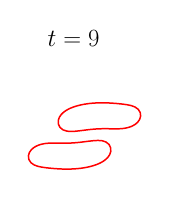
\begin{tikzpicture}[scale=0.36]

\begin{axis}[
  xmin = -6,
  xmax = 2,
  ymin = -2,
  ymax = 2,
  axis equal = true,
  hide axis,
  title = {\Huge$t=9$}
  ]

\addplot [mark=none,red,line width=1.5] table{
1.1293e-02 3.5515e-01
6.8710e-02 3.6215e-01
1.3014e-01 3.7188e-01
1.9860e-01 3.8587e-01
2.7564e-01 4.0621e-01
3.6133e-01 4.3570e-01
4.5413e-01 4.7795e-01
5.5039e-01 5.3756e-01
6.4311e-01 6.1992e-01
7.1971e-01 7.2986e-01
7.6035e-01 8.6675e-01
7.4279e-01 1.0160e+00
6.5937e-01 1.1488e+00
5.2691e-01 1.2433e+00
3.6980e-01 1.3009e+00
2.0294e-01 1.3355e+00
3.2641e-02 1.3593e+00
-1.3832e-01 1.3779e+00
-3.0814e-01 1.3931e+00
-4.7534e-01 1.4046e+00
-6.3842e-01 1.4121e+00
-7.9596e-01 1.4151e+00
-9.4656e-01 1.4137e+00
-1.0889e+00 1.4081e+00
-1.2218e+00 1.3989e+00
-1.3443e+00 1.3868e+00
-1.4556e+00 1.3724e+00
-1.5553e+00 1.3566e+00
-1.6434e+00 1.3402e+00
-1.7206e+00 1.3237e+00
-1.7879e+00 1.3075e+00
-1.8477e+00 1.2917e+00
-1.9031e+00 1.2756e+00
-1.9582e+00 1.2582e+00
-2.0169e+00 1.2380e+00
-2.0821e+00 1.2131e+00
-2.1552e+00 1.1817e+00
-2.2364e+00 1.1415e+00
-2.3243e+00 1.0899e+00
-2.4158e+00 1.0233e+00
-2.5052e+00 9.3730e-01
-2.5823e+00 8.2757e-01
-2.6305e+00 6.9290e-01
-2.6282e+00 5.4233e-01
-2.5600e+00 4.0103e-01
-2.4335e+00 2.9918e-01
-2.2747e+00 2.4762e-01
-2.1049e+00 2.3468e-01
-1.9333e+00 2.4342e-01
-1.7624e+00 2.6182e-01
-1.5934e+00 2.8315e-01
-1.4271e+00 3.0372e-01
-1.2649e+00 3.2136e-01
-1.1080e+00 3.3478e-01
-9.5775e-01 3.4344e-01
-8.1541e-01 3.4760e-01
-6.8220e-01 3.4821e-01
-5.5912e-01 3.4667e-01
-4.4687e-01 3.4446e-01
-3.4588e-01 3.4278e-01
-2.5617e-01 3.4236e-01
-1.7726e-01 3.4347e-01
-1.0798e-01 3.4605e-01
-4.6213e-02 3.4993e-01
1.1293e-02 3.5515e-01
};

\addplot [mark=none,red,line width=1.5] table{
-1.1969e+00 -1.1756e+00
-1.1418e+00 -1.1582e+00
-1.0831e+00 -1.1380e+00
-1.0179e+00 -1.1131e+00
-9.4477e-01 -1.0817e+00
-8.6361e-01 -1.0415e+00
-7.7574e-01 -9.8990e-01
-6.8421e-01 -9.2329e-01
-5.9480e-01 -8.3730e-01
-5.1770e-01 -7.2757e-01
-4.6950e-01 -5.9290e-01
-4.7182e-01 -4.4233e-01
-5.3999e-01 -3.0103e-01
-6.6646e-01 -1.9918e-01
-8.2531e-01 -1.4762e-01
-9.9505e-01 -1.3468e-01
-1.1667e+00 -1.4342e-01
-1.3376e+00 -1.6182e-01
-1.5066e+00 -1.8315e-01
-1.6729e+00 -2.0372e-01
-1.8351e+00 -2.2136e-01
-1.9920e+00 -2.3478e-01
-2.1423e+00 -2.4344e-01
-2.2846e+00 -2.4760e-01
-2.4178e+00 -2.4821e-01
-2.5409e+00 -2.4667e-01
-2.6531e+00 -2.4446e-01
-2.7541e+00 -2.4278e-01
-2.8438e+00 -2.4236e-01
-2.9227e+00 -2.4347e-01
-2.9920e+00 -2.4605e-01
-3.0538e+00 -2.4993e-01
-3.1113e+00 -2.5515e-01
-3.1687e+00 -2.6215e-01
-3.2301e+00 -2.7188e-01
-3.2986e+00 -2.8587e-01
-3.3756e+00 -3.0621e-01
-3.4613e+00 -3.3570e-01
-3.5541e+00 -3.7795e-01
-3.6504e+00 -4.3756e-01
-3.7431e+00 -5.1992e-01
-3.8197e+00 -6.2986e-01
-3.8604e+00 -7.6675e-01
-3.8428e+00 -9.1603e-01
-3.7594e+00 -1.0488e+00
-3.6269e+00 -1.1433e+00
-3.4698e+00 -1.2009e+00
-3.3029e+00 -1.2355e+00
-3.1326e+00 -1.2593e+00
-2.9617e+00 -1.2779e+00
-2.7919e+00 -1.2931e+00
-2.6247e+00 -1.3046e+00
-2.4616e+00 -1.3121e+00
-2.3040e+00 -1.3151e+00
-2.1534e+00 -1.3137e+00
-2.0111e+00 -1.3081e+00
-1.8782e+00 -1.2989e+00
-1.7557e+00 -1.2868e+00
-1.6444e+00 -1.2724e+00
-1.5447e+00 -1.2566e+00
-1.4566e+00 -1.2402e+00
-1.3794e+00 -1.2237e+00
-1.3121e+00 -1.2075e+00
-1.2523e+00 -1.1917e+00
-1.1969e+00 -1.1756e+00
};

\end{axis}
\end{tikzpicture}

 &
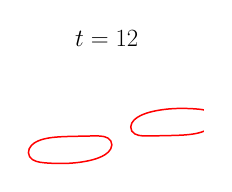
\begin{tikzpicture}[scale=0.36]

\begin{axis}[
  xmin = -6,
  xmax = 2,
  ymin = -2,
  ymax = 2,
  axis equal = true,
  hide axis,
  title = {\Huge$t=12$}
  ]

\addplot [mark=none,red,line width=1.5] table{
1.0896e+00 8.3914e-02
1.1473e+00 8.7321e-02
1.2094e+00 9.1519e-02
1.2790e+00 9.6982e-02
1.3584e+00 1.0433e-01
1.4485e+00 1.1438e-01
1.5496e+00 1.2823e-01
1.6614e+00 1.4744e-01
1.7828e+00 1.7420e-01
1.9122e+00 2.1161e-01
2.0463e+00 2.6411e-01
2.1794e+00 3.3777e-01
2.3011e+00 4.4003e-01
2.3921e+00 5.7642e-01
2.4242e+00 7.4070e-01
2.3752e+00 9.0283e-01
2.2557e+00 1.0251e+00
2.1001e+00 1.0972e+00
1.9339e+00 1.1347e+00
1.7676e+00 1.1549e+00
1.6048e+00 1.1674e+00
1.4475e+00 1.1759e+00
1.2969e+00 1.1814e+00
1.1545e+00 1.1840e+00
1.0213e+00 1.1839e+00
8.9820e-01 1.1814e+00
7.8604e-01 1.1769e+00
6.8524e-01 1.1711e+00
5.9581e-01 1.1644e+00
5.1725e-01 1.1574e+00
4.4833e-01 1.1503e+00
3.8690e-01 1.1433e+00
3.2966e-01 1.1361e+00
2.7241e-01 1.1283e+00
2.1094e-01 1.1192e+00
1.4203e-01 1.1080e+00
6.3637e-02 1.0940e+00
-2.5214e-02 1.0764e+00
-1.2476e-01 1.0542e+00
-2.3456e-01 1.0262e+00
-3.5370e-01 9.9069e-01
-4.8045e-01 9.4546e-01
-6.1215e-01 8.8727e-01
-7.4413e-01 8.1152e-01
-8.6796e-01 7.1170e-01
-9.6691e-01 5.8061e-01
-1.0112e+00 4.1904e-01
-9.6919e-01 2.5518e-01
-8.4733e-01 1.3585e-01
-6.8709e-01 7.5285e-02
-5.1822e-01 5.3156e-02
-3.5079e-01 4.8692e-02
-1.8760e-01 5.0418e-02
-3.0136e-02 5.3747e-02
1.2039e-01 5.7078e-02
2.6276e-01 6.0082e-02
3.9597e-01 6.2762e-02
5.1903e-01 6.5260e-02
6.3128e-01 6.7702e-02
7.3224e-01 7.0186e-02
8.2193e-01 7.2755e-02
9.0080e-01 7.5406e-02
9.7009e-01 7.8126e-02
1.0319e+00 8.0925e-02
1.0896e+00 8.3914e-02
};

\addplot [mark=none,red,line width=1.5] table{
-3.1297e+00 -1.0361e+00
-3.0724e+00 -1.0283e+00
-3.0109e+00 -1.0192e+00
-2.9420e+00 -1.0080e+00
-2.8636e+00 -9.9402e-01
-2.7748e+00 -9.7642e-01
-2.6752e+00 -9.5422e-01
-2.5654e+00 -9.2619e-01
-2.4463e+00 -8.9069e-01
-2.3195e+00 -8.4546e-01
-2.1879e+00 -7.8727e-01
-2.0559e+00 -7.1152e-01
-1.9320e+00 -6.1170e-01
-1.8331e+00 -4.8061e-01
-1.7888e+00 -3.1904e-01
-1.8308e+00 -1.5518e-01
-1.9527e+00 -3.5847e-02
-2.1129e+00 2.4716e-02
-2.2818e+00 4.6844e-02
-2.4492e+00 5.1308e-02
-2.6124e+00 4.9582e-02
-2.7699e+00 4.6253e-02
-2.9204e+00 4.2922e-02
-3.0628e+00 3.9918e-02
-3.1960e+00 3.7238e-02
-3.3190e+00 3.4740e-02
-3.4313e+00 3.2298e-02
-3.5322e+00 2.9814e-02
-3.6219e+00 2.7245e-02
-3.7008e+00 2.4594e-02
-3.7701e+00 2.1874e-02
-3.8319e+00 1.9075e-02
-3.8896e+00 1.6086e-02
-3.9473e+00 1.2679e-02
-4.0094e+00 8.4808e-03
-4.0790e+00 3.0180e-03
-4.1584e+00 -4.3319e-03
-4.2485e+00 -1.4377e-02
-4.3496e+00 -2.8233e-02
-4.4614e+00 -4.7442e-02
-4.5828e+00 -7.4195e-02
-4.7122e+00 -1.1161e-01
-4.8463e+00 -1.6411e-01
-4.9794e+00 -2.3777e-01
-5.1011e+00 -3.4003e-01
-5.1921e+00 -4.7642e-01
-5.2242e+00 -6.4070e-01
-5.1752e+00 -8.0283e-01
-5.0557e+00 -9.2508e-01
-4.9001e+00 -9.9721e-01
-4.7339e+00 -1.0347e+00
-4.5676e+00 -1.0549e+00
-4.4048e+00 -1.0674e+00
-4.2475e+00 -1.0759e+00
-4.0969e+00 -1.0814e+00
-3.9545e+00 -1.0840e+00
-3.8213e+00 -1.0839e+00
-3.6982e+00 -1.0814e+00
-3.5860e+00 -1.0769e+00
-3.4852e+00 -1.0711e+00
-3.3958e+00 -1.0644e+00
-3.3173e+00 -1.0574e+00
-3.2483e+00 -1.0503e+00
-3.1869e+00 -1.0433e+00
-3.1297e+00 -1.0361e+00
};

\end{axis}
\end{tikzpicture}

 \\
$\nu=1$ &
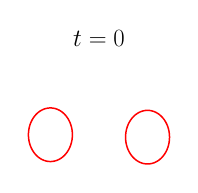
\begin{tikzpicture}[scale=0.36]

\begin{axis}[
  xmin = -6,
  xmax = 2,
  ymin = -2,
  ymax = 2,
  axis equal = true,
  hide axis,
  title = {\Huge$t=0$}
  ]

\addplot [mark=none,red,line width=1.5] table{
-4.0000e+00 1.2044e+00
-4.0888e+00 1.1991e+00
-4.1766e+00 1.1832e+00
-4.2628e+00 1.1568e+00
-4.3465e+00 1.1203e+00
-4.4268e+00 1.0740e+00
-4.5031e+00 1.0183e+00
-4.5744e+00 9.5370e-01
-4.6403e+00 8.8092e-01
-4.6999e+00 8.0062e-01
-4.7529e+00 7.1357e-01
-4.7986e+00 6.2061e-01
-4.8366e+00 5.2263e-01
-4.8665e+00 4.2059e-01
-4.8881e+00 3.1546e-01
-4.9011e+00 2.0825e-01
-4.9055e+00 1.0000e-01
-4.9011e+00 -8.2491e-03
-4.8881e+00 -1.1546e-01
-4.8665e+00 -2.2059e-01
-4.8366e+00 -3.2263e-01
-4.7986e+00 -4.2061e-01
-4.7529e+00 -5.1357e-01
-4.6999e+00 -6.0062e-01
-4.6403e+00 -6.8092e-01
-4.5744e+00 -7.5370e-01
-4.5031e+00 -8.1827e-01
-4.4268e+00 -8.7398e-01
-4.3465e+00 -9.2032e-01
-4.2628e+00 -9.5683e-01
-4.1766e+00 -9.8317e-01
-4.0888e+00 -9.9907e-01
-4.0000e+00 -1.0044e+00
-3.9112e+00 -9.9907e-01
-3.8234e+00 -9.8317e-01
-3.7372e+00 -9.5683e-01
-3.6535e+00 -9.2032e-01
-3.5732e+00 -8.7398e-01
-3.4969e+00 -8.1827e-01
-3.4256e+00 -7.5370e-01
-3.3597e+00 -6.8092e-01
-3.3001e+00 -6.0062e-01
-3.2471e+00 -5.1357e-01
-3.2014e+00 -4.2061e-01
-3.1634e+00 -3.2263e-01
-3.1335e+00 -2.2059e-01
-3.1119e+00 -1.1546e-01
-3.0989e+00 -8.2491e-03
-3.0945e+00 1.0000e-01
-3.0989e+00 2.0825e-01
-3.1119e+00 3.1546e-01
-3.1335e+00 4.2059e-01
-3.1634e+00 5.2263e-01
-3.2014e+00 6.2061e-01
-3.2471e+00 7.1357e-01
-3.3001e+00 8.0062e-01
-3.3597e+00 8.8092e-01
-3.4256e+00 9.5370e-01
-3.4969e+00 1.0183e+00
-3.5732e+00 1.0740e+00
-3.6535e+00 1.1203e+00
-3.7372e+00 1.1568e+00
-3.8234e+00 1.1832e+00
-3.9112e+00 1.1991e+00
-4.0000e+00 1.2044e+00
};

\addplot [mark=none,red,line width=1.5] table{
6.7624e-17 1.1044e+00
-8.8752e-02 1.0991e+00
-1.7665e-01 1.0832e+00
-2.6285e-01 1.0568e+00
-3.4651e-01 1.0203e+00
-4.2684e-01 9.7398e-01
-5.0306e-01 9.1827e-01
-5.7443e-01 8.5370e-01
-6.4027e-01 7.8092e-01
-6.9994e-01 7.0062e-01
-7.5288e-01 6.1357e-01
-7.9856e-01 5.2061e-01
-8.3655e-01 4.2263e-01
-8.6649e-01 3.2059e-01
-8.8808e-01 2.1546e-01
-9.0112e-01 1.0825e-01
-9.0548e-01 1.2307e-16
-9.0112e-01 -1.0825e-01
-8.8808e-01 -2.1546e-01
-8.6649e-01 -3.2059e-01
-8.3655e-01 -4.2263e-01
-7.9856e-01 -5.2061e-01
-7.5288e-01 -6.1357e-01
-6.9994e-01 -7.0062e-01
-6.4027e-01 -7.8092e-01
-5.7443e-01 -8.5370e-01
-5.0306e-01 -9.1827e-01
-4.2684e-01 -9.7398e-01
-3.4651e-01 -1.0203e+00
-2.6285e-01 -1.0568e+00
-1.7665e-01 -1.0832e+00
-8.8752e-02 -1.0991e+00
-1.7851e-16 -1.1044e+00
8.8752e-02 -1.0991e+00
1.7665e-01 -1.0832e+00
2.6285e-01 -1.0568e+00
3.4651e-01 -1.0203e+00
4.2684e-01 -9.7398e-01
5.0306e-01 -9.1827e-01
5.7443e-01 -8.5370e-01
6.4027e-01 -7.8092e-01
6.9994e-01 -7.0062e-01
7.5288e-01 -6.1357e-01
7.9856e-01 -5.2061e-01
8.3655e-01 -4.2263e-01
8.6649e-01 -3.2059e-01
8.8808e-01 -2.1546e-01
9.0112e-01 -1.0825e-01
9.0548e-01 -2.5832e-16
9.0112e-01 1.0825e-01
8.8808e-01 2.1546e-01
8.6649e-01 3.2059e-01
8.3655e-01 4.2263e-01
7.9856e-01 5.2061e-01
7.5288e-01 6.1357e-01
6.9994e-01 7.0062e-01
6.4027e-01 7.8092e-01
5.7443e-01 8.5370e-01
5.0306e-01 9.1827e-01
4.2684e-01 9.7398e-01
3.4651e-01 1.0203e+00
2.6285e-01 1.0568e+00
1.7665e-01 1.0832e+00
8.8752e-02 1.0991e+00
6.7624e-17 1.1044e+00
};

\end{axis}
\end{tikzpicture}

 &
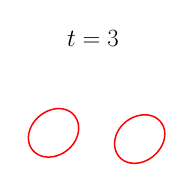
\begin{tikzpicture}[scale=0.36]

\begin{axis}[
  xmin = -6,
  xmax = 2,
  ymin = -2,
  ymax = 2,
  axis equal = true,
  hide axis,
  title = {\Huge$t=3$}
  ]

\addplot [mark=none,red,line width=1.5] table{
-2.5977e+00 4.8832e-01
-2.6136e+00 5.7651e-01
-2.6390e+00 6.6290e-01
-2.6741e+00 7.4667e-01
-2.7193e+00 8.2673e-01
-2.7749e+00 9.0180e-01
-2.8407e+00 9.7040e-01
-2.9162e+00 1.0310e+00
-3.0006e+00 1.0823e+00
-3.0927e+00 1.1232e+00
-3.1908e+00 1.1528e+00
-3.2934e+00 1.1708e+00
-3.3989e+00 1.1772e+00
-3.5058e+00 1.1723e+00
-3.6126e+00 1.1566e+00
-3.7181e+00 1.1307e+00
-3.8212e+00 1.0955e+00
-3.9209e+00 1.0515e+00
-4.0164e+00 9.9983e-01
-4.1070e+00 9.4111e-01
-4.1920e+00 8.7622e-01
-4.2709e+00 8.0594e-01
-4.3432e+00 7.3105e-01
-4.4087e+00 6.5227e-01
-4.4670e+00 5.7028e-01
-4.5179e+00 4.8570e-01
-4.5613e+00 3.9909e-01
-4.5968e+00 3.1095e-01
-4.6245e+00 2.2175e-01
-4.6441e+00 1.3188e-01
-4.6553e+00 4.1744e-02
-4.6579e+00 -4.8257e-02
-4.6515e+00 -1.3765e-01
-4.6357e+00 -2.2587e-01
-4.6101e+00 -3.1216e-01
-4.5742e+00 -3.9558e-01
-4.5279e+00 -4.7501e-01
-4.4711e+00 -5.4913e-01
-4.4041e+00 -6.1654e-01
-4.3275e+00 -6.7589e-01
-4.2424e+00 -7.2598e-01
-4.1500e+00 -7.6586e-01
-4.0517e+00 -7.9493e-01
-3.9490e+00 -8.1287e-01
-3.8435e+00 -8.1970e-01
-3.7366e+00 -8.1563e-01
-3.6297e+00 -8.0109e-01
-3.5238e+00 -7.7659e-01
-3.4202e+00 -7.4276e-01
-3.3199e+00 -7.0027e-01
-3.2237e+00 -6.4983e-01
-3.1325e+00 -5.9217e-01
-3.0469e+00 -5.2805e-01
-2.9676e+00 -4.5823e-01
-2.8951e+00 -3.8347e-01
-2.8299e+00 -3.0454e-01
-2.7721e+00 -2.2217e-01
-2.7221e+00 -1.3705e-01
-2.6801e+00 -4.9854e-02
-2.6460e+00 3.8837e-02
-2.6199e+00 1.2850e-01
-2.6019e+00 2.1867e-01
-2.5921e+00 3.0896e-01
-2.5906e+00 3.9898e-01
-2.5977e+00 4.8832e-01
};

\addplot [mark=none,red,line width=1.5] table{
9.5150e-01 2.3765e-01
9.3570e-01 3.2587e-01
9.1006e-01 4.1216e-01
8.7420e-01 4.9558e-01
8.2788e-01 5.7501e-01
7.7107e-01 6.4913e-01
7.0408e-01 7.1654e-01
6.2752e-01 7.7589e-01
5.4241e-01 8.2598e-01
4.4998e-01 8.6586e-01
3.5169e-01 8.9493e-01
2.4904e-01 9.1287e-01
1.4355e-01 9.1970e-01
3.6642e-02 9.1563e-01
-7.0337e-02 9.0109e-01
-1.7617e-01 8.7659e-01
-2.7976e-01 8.4276e-01
-3.8009e-01 8.0027e-01
-4.7628e-01 7.4983e-01
-5.6751e-01 6.9217e-01
-6.5308e-01 6.2805e-01
-7.3237e-01 5.5823e-01
-8.0486e-01 4.8347e-01
-8.7014e-01 4.0454e-01
-9.2788e-01 3.2217e-01
-9.7786e-01 2.3705e-01
-1.0199e+00 1.4985e-01
-1.0540e+00 6.1163e-02
-1.0801e+00 -2.8498e-02
-1.0981e+00 -1.1867e-01
-1.1079e+00 -2.0896e-01
-1.1094e+00 -2.9898e-01
-1.1023e+00 -3.8832e-01
-1.0864e+00 -4.7651e-01
-1.0610e+00 -5.6290e-01
-1.0259e+00 -6.4667e-01
-9.8069e-01 -7.2673e-01
-9.2511e-01 -8.0180e-01
-8.5931e-01 -8.7040e-01
-7.8377e-01 -9.3104e-01
-6.9936e-01 -9.8234e-01
-6.0735e-01 -1.0232e+00
-5.0922e-01 -1.0528e+00
-4.0659e-01 -1.0708e+00
-3.0107e-01 -1.0772e+00
-1.9420e-01 -1.0723e+00
-8.7390e-02 -1.0566e+00
1.8121e-02 -1.0307e+00
1.2122e-01 -9.9546e-01
2.2094e-01 -9.5155e-01
3.1645e-01 -8.9983e-01
4.0700e-01 -8.4111e-01
4.9198e-01 -7.7622e-01
5.7087e-01 -7.0594e-01
6.4323e-01 -6.3105e-01
7.0870e-01 -5.5227e-01
7.6701e-01 -4.7028e-01
8.1793e-01 -3.8570e-01
8.6126e-01 -2.9909e-01
8.9685e-01 -2.1095e-01
9.2452e-01 -1.2175e-01
9.4408e-01 -3.1882e-02
9.5531e-01 5.8256e-02
9.5790e-01 1.4826e-01
9.5150e-01 2.3765e-01
};

\end{axis}
\end{tikzpicture}

 &
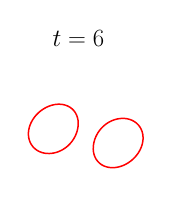
\begin{tikzpicture}[scale=0.36]

\begin{axis}[
  xmin = -6,
  xmax = 2,
  ymin = -2,
  ymax = 2,
  axis equal = true,
  hide axis,
  title = {\Huge$t=6$}
  ]

\addplot [mark=none,red,line width=1.5] table{
-2.5082e+00 -4.1872e-01
-2.4390e+00 -3.6122e-01
-2.3736e+00 -2.9869e-01
-2.3123e+00 -2.3109e-01
-2.2552e+00 -1.5840e-01
-2.2026e+00 -8.0595e-02
-2.1548e+00 2.2781e-03
-2.1124e+00 9.0108e-02
-2.0759e+00 1.8269e-01
-2.0463e+00 2.7970e-01
-2.0244e+00 3.8068e-01
-2.0115e+00 4.8492e-01
-2.0089e+00 5.9144e-01
-2.0179e+00 6.9888e-01
-2.0400e+00 8.0538e-01
-2.0762e+00 9.0861e-01
-2.1269e+00 1.0059e+00
-2.1915e+00 1.0944e+00
-2.2686e+00 1.1717e+00
-2.3559e+00 1.2358e+00
-2.4508e+00 1.2861e+00
-2.5504e+00 1.3223e+00
-2.6524e+00 1.3452e+00
-2.7545e+00 1.3558e+00
-2.8554e+00 1.3556e+00
-2.9539e+00 1.3458e+00
-3.0493e+00 1.3276e+00
-3.1412e+00 1.3021e+00
-3.2293e+00 1.2702e+00
-3.3135e+00 1.2327e+00
-3.3940e+00 1.1900e+00
-3.4709e+00 1.1424e+00
-3.5442e+00 1.0902e+00
-3.6140e+00 1.0335e+00
-3.6804e+00 9.7208e-01
-3.7433e+00 9.0594e-01
-3.8025e+00 8.3489e-01
-3.8576e+00 7.5876e-01
-3.9081e+00 6.7745e-01
-3.9531e+00 5.9093e-01
-3.9919e+00 4.9929e-01
-4.0233e+00 4.0282e-01
-4.0460e+00 3.0204e-01
-4.0588e+00 1.9779e-01
-4.0601e+00 9.1271e-02
-4.0487e+00 -1.5902e-02
-4.0236e+00 -1.2169e-01
-3.9843e+00 -2.2370e-01
-3.9308e+00 -3.1938e-01
-3.8640e+00 -4.0624e-01
-3.7857e+00 -4.8218e-01
-3.6979e+00 -5.4575e-01
-3.6031e+00 -5.9620e-01
-3.5039e+00 -6.3352e-01
-3.4024e+00 -6.5821e-01
-3.3004e+00 -6.7117e-01
-3.1995e+00 -6.7345e-01
-3.1008e+00 -6.6616e-01
-3.0050e+00 -6.5035e-01
-2.9126e+00 -6.2696e-01
-2.8239e+00 -5.9679e-01
-2.7391e+00 -5.6047e-01
-2.6582e+00 -5.1849e-01
-2.5813e+00 -4.7117e-01
-2.5082e+00 -4.1872e-01
};

\addplot [mark=none,red,line width=1.5] table{
1.4417e-01 -9.9023e-01
2.1402e-01 -9.3347e-01
2.8044e-01 -8.7208e-01
3.4335e-01 -8.0594e-01
4.0253e-01 -7.3489e-01
4.5762e-01 -6.5876e-01
5.0806e-01 -5.7745e-01
5.5313e-01 -4.9093e-01
5.9191e-01 -3.9929e-01
6.2329e-01 -3.0282e-01
6.4602e-01 -2.0204e-01
6.5875e-01 -9.7791e-02
6.6009e-01 8.7287e-03
6.4872e-01 1.1590e-01
6.2364e-01 2.2169e-01
5.8429e-01 3.2370e-01
5.3080e-01 4.1938e-01
4.6404e-01 5.0624e-01
3.8567e-01 5.8218e-01
2.9788e-01 6.4575e-01
2.0313e-01 6.9620e-01
1.0388e-01 7.3352e-01
2.3623e-03 7.5821e-01
-9.9573e-02 7.7117e-01
-2.0045e-01 7.7345e-01
-2.9919e-01 7.6616e-01
-3.9501e-01 7.5035e-01
-4.8741e-01 7.2696e-01
-5.7608e-01 6.9679e-01
-6.6088e-01 6.6047e-01
-7.4176e-01 6.1849e-01
-8.1873e-01 5.7117e-01
-8.9182e-01 5.1872e-01
-9.6105e-01 4.6122e-01
-1.0264e+00 3.9869e-01
-1.0877e+00 3.3109e-01
-1.1448e+00 2.5840e-01
-1.1974e+00 1.8060e-01
-1.2452e+00 9.7722e-02
-1.2876e+00 9.8920e-03
-1.3241e+00 -8.2690e-02
-1.3537e+00 -1.7970e-01
-1.3756e+00 -2.8068e-01
-1.3885e+00 -3.8492e-01
-1.3911e+00 -4.9144e-01
-1.3821e+00 -5.9888e-01
-1.3600e+00 -7.0538e-01
-1.3238e+00 -8.0861e-01
-1.2731e+00 -9.0588e-01
-1.2085e+00 -9.9439e-01
-1.1314e+00 -1.0717e+00
-1.0441e+00 -1.1358e+00
-9.4922e-01 -1.1861e+00
-8.4958e-01 -1.2223e+00
-7.4765e-01 -1.2452e+00
-6.4546e-01 -1.2558e+00
-5.4457e-01 -1.2556e+00
-4.4605e-01 -1.2458e+00
-3.5066e-01 -1.2276e+00
-2.5881e-01 -1.2021e+00
-1.7072e-01 -1.1702e+00
-8.6457e-02 -1.1327e+00
-5.9586e-03 -1.0900e+00
7.0878e-02 -1.0424e+00
1.4417e-01 -9.9023e-01
};

\end{axis}
\end{tikzpicture}

 &
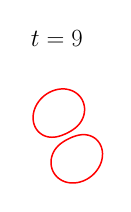
\begin{tikzpicture}[scale=0.36]

\begin{axis}[
  xmin = -6,
  xmax = 2,
  ymin = -2,
  ymax = 2,
  axis equal = true,
  hide axis,
  title = {\Huge$t=9$}
  ]

\addplot [mark=none,red,line width=1.5] table{
-2.6374e+00 1.2421e-01
-2.5592e+00 7.8773e-02
-2.4757e+00 4.2962e-02
-2.3878e+00 1.7103e-02
-2.2963e+00 1.4030e-03
-2.2022e+00 -4.0951e-03
-2.1063e+00 4.2682e-04
-2.0095e+00 1.4495e-02
-1.9123e+00 3.7313e-02
-1.8152e+00 6.7827e-02
-1.7184e+00 1.0489e-01
-1.6219e+00 1.4755e-01
-1.5261e+00 1.9525e-01
-1.4315e+00 2.4808e-01
-1.3391e+00 3.0661e-01
-1.2504e+00 3.7171e-01
-1.1671e+00 4.4413e-01
-1.0911e+00 5.2414e-01
-1.0241e+00 6.1135e-01
-9.6752e-01 7.0480e-01
-9.2231e-01 8.0310e-01
-8.8901e-01 9.0466e-01
-8.6787e-01 1.0078e+00
-8.5884e-01 1.1110e+00
-8.6169e-01 1.2127e+00
-8.7598e-01 1.3114e+00
-9.0110e-01 1.4060e+00
-9.3632e-01 1.4953e+00
-9.8080e-01 1.5785e+00
-1.0337e+00 1.6548e+00
-1.0940e+00 1.7238e+00
-1.1611e+00 1.7852e+00
-1.2340e+00 1.8387e+00
-1.3122e+00 1.8842e+00
-1.3950e+00 1.9215e+00
-1.4820e+00 1.9507e+00
-1.5725e+00 1.9715e+00
-1.6660e+00 1.9838e+00
-1.7620e+00 1.9875e+00
-1.8598e+00 1.9824e+00
-1.9587e+00 1.9684e+00
-2.0579e+00 1.9454e+00
-2.1565e+00 1.9135e+00
-2.2538e+00 1.8728e+00
-2.3487e+00 1.8234e+00
-2.4402e+00 1.7656e+00
-2.5275e+00 1.6999e+00
-2.6095e+00 1.6267e+00
-2.6854e+00 1.5466e+00
-2.7542e+00 1.4605e+00
-2.8151e+00 1.3690e+00
-2.8673e+00 1.2731e+00
-2.9103e+00 1.1738e+00
-2.9433e+00 1.0721e+00
-2.9661e+00 9.6930e-01
-2.9783e+00 8.6641e-01
-2.9798e+00 7.6469e-01
-2.9706e+00 6.6531e-01
-2.9508e+00 5.6946e-01
-2.9207e+00 4.7824e-01
-2.8809e+00 3.9270e-01
-2.8320e+00 3.1377e-01
-2.7746e+00 2.4226e-01
-2.7094e+00 1.7888e-01
-2.6374e+00 1.2421e-01
};

\addplot [mark=none,red,line width=1.5] table{
-1.8660e+00 -1.7387e+00
-1.7878e+00 -1.7842e+00
-1.7050e+00 -1.8215e+00
-1.6180e+00 -1.8507e+00
-1.5275e+00 -1.8715e+00
-1.4340e+00 -1.8838e+00
-1.3380e+00 -1.8875e+00
-1.2402e+00 -1.8824e+00
-1.1413e+00 -1.8684e+00
-1.0421e+00 -1.8454e+00
-9.4346e-01 -1.8135e+00
-8.4621e-01 -1.7728e+00
-7.5132e-01 -1.7234e+00
-6.5975e-01 -1.6656e+00
-5.7248e-01 -1.5999e+00
-4.9046e-01 -1.5267e+00
-4.1461e-01 -1.4466e+00
-3.4583e-01 -1.3605e+00
-2.8494e-01 -1.2690e+00
-2.3269e-01 -1.1731e+00
-1.8974e-01 -1.0738e+00
-1.5666e-01 -9.7215e-01
-1.3386e-01 -8.6930e-01
-1.2165e-01 -7.6641e-01
-1.2018e-01 -6.6469e-01
-1.2943e-01 -5.6531e-01
-1.4924e-01 -4.6946e-01
-1.7928e-01 -3.7824e-01
-2.1907e-01 -2.9270e-01
-2.6801e-01 -2.1377e-01
-3.2543e-01 -1.4226e-01
-3.9056e-01 -7.8876e-02
-4.6263e-01 -2.4215e-02
-5.4081e-01 2.1227e-02
-6.2429e-01 5.7038e-02
-7.1221e-01 8.2897e-02
-8.0367e-01 9.8597e-02
-8.9778e-01 1.0410e-01
-9.9366e-01 9.9573e-02
-1.0905e+00 8.5505e-02
-1.1877e+00 6.2687e-02
-1.2848e+00 3.2173e-02
-1.3816e+00 -4.8930e-03
-1.4781e+00 -4.7545e-02
-1.5739e+00 -9.5255e-02
-1.6685e+00 -1.4808e-01
-1.7609e+00 -2.0661e-01
-1.8496e+00 -2.7171e-01
-1.9329e+00 -3.4413e-01
-2.0089e+00 -4.2414e-01
-2.0759e+00 -5.1135e-01
-2.1325e+00 -6.0480e-01
-2.1777e+00 -7.0310e-01
-2.2110e+00 -8.0466e-01
-2.2321e+00 -9.0783e-01
-2.2412e+00 -1.0110e+00
-2.2383e+00 -1.1127e+00
-2.2240e+00 -1.2114e+00
-2.1989e+00 -1.3060e+00
-2.1637e+00 -1.3953e+00
-2.1192e+00 -1.4785e+00
-2.0663e+00 -1.5548e+00
-2.0060e+00 -1.6238e+00
-1.9389e+00 -1.6852e+00
-1.8660e+00 -1.7387e+00
};

\end{axis}
\end{tikzpicture}

 &
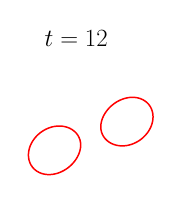
\begin{tikzpicture}[scale=0.36]

\begin{axis}[
  xmin = -6,
  xmax = 2,
  ymin = -2,
  ymax = 2,
  axis equal = true,
  hide axis,
  title = {\Huge$t=12$}
  ]

\addplot [mark=none,red,line width=1.5] table{
-6.3844e-01 1.2046e+00
-6.9949e-01 1.1364e+00
-7.5633e-01 1.0640e+00
-8.0872e-01 9.8729e-01
-8.5621e-01 9.0600e-01
-8.9812e-01 8.1999e-01
-9.3348e-01 7.2920e-01
-9.6102e-01 6.3378e-01
-9.7916e-01 5.3420e-01
-9.8610e-01 4.3135e-01
-9.7999e-01 3.2666e-01
-9.5925e-01 2.2218e-01
-9.2299e-01 1.2048e-01
-8.7127e-01 2.4308e-02
-8.0519e-01 -6.3788e-02
-7.2658e-01 -1.4181e-01
-6.3773e-01 -2.0841e-01
-5.4100e-01 -2.6284e-01
-4.3869e-01 -3.0483e-01
-3.3293e-01 -3.3454e-01
-2.2557e-01 -3.5244e-01
-1.1826e-01 -3.5920e-01
-1.2331e-02 -3.5569e-01
9.1146e-02 -3.4284e-01
1.9135e-01 -3.2158e-01
2.8770e-01 -2.9284e-01
3.7979e-01 -2.5744e-01
4.6740e-01 -2.1611e-01
5.5042e-01 -1.6947e-01
6.2882e-01 -1.1799e-01
7.0267e-01 -6.1985e-02
7.7201e-01 -1.6670e-03
8.3687e-01 6.2896e-02
8.9722e-01 1.3173e-01
9.5293e-01 2.0493e-01
1.0037e+00 2.8264e-01
1.0491e+00 3.6499e-01
1.0885e+00 4.5201e-01
1.1210e+00 5.4367e-01
1.1456e+00 6.3970e-01
1.1610e+00 7.3958e-01
1.1660e+00 8.4247e-01
1.1590e+00 9.4709e-01
1.1389e+00 1.0517e+00
1.1048e+00 1.1542e+00
1.0561e+00 1.2520e+00
9.9338e-01 1.3425e+00
9.1762e-01 1.4233e+00
8.3071e-01 1.4924e+00
7.3497e-01 1.5485e+00
6.3293e-01 1.5911e+00
5.2703e-01 1.6202e+00
4.1947e-01 1.6367e+00
3.1207e-01 1.6413e+00
2.0627e-01 1.6354e+00
1.0316e-01 1.6200e+00
3.5368e-03 1.5963e+00
-9.2089e-02 1.5653e+00
-1.8339e-01 1.5281e+00
-2.7022e-01 1.4853e+00
-3.5255e-01 1.4376e+00
-4.3043e-01 1.3854e+00
-5.0396e-01 1.3291e+00
-5.7327e-01 1.2688e+00
-6.3844e-01 1.2046e+00
};

\addplot [mark=none,red,line width=1.5] table{
-3.6369e+00 3.7104e-02
-3.6972e+00 -3.1729e-02
-3.7529e+00 -1.0493e-01
-3.8037e+00 -1.8264e-01
-3.8491e+00 -2.6499e-01
-3.8885e+00 -3.5201e-01
-3.9210e+00 -4.4367e-01
-3.9456e+00 -5.3970e-01
-3.9610e+00 -6.3958e-01
-3.9660e+00 -7.4247e-01
-3.9590e+00 -8.4709e-01
-3.9389e+00 -9.5171e-01
-3.9048e+00 -1.0542e+00
-3.8561e+00 -1.1520e+00
-3.7934e+00 -1.2425e+00
-3.7176e+00 -1.3233e+00
-3.6307e+00 -1.3924e+00
-3.5350e+00 -1.4485e+00
-3.4329e+00 -1.4911e+00
-3.3270e+00 -1.5202e+00
-3.2195e+00 -1.5367e+00
-3.1121e+00 -1.5413e+00
-3.0063e+00 -1.5354e+00
-2.9032e+00 -1.5200e+00
-2.8035e+00 -1.4963e+00
-2.7079e+00 -1.4653e+00
-2.6166e+00 -1.4281e+00
-2.5298e+00 -1.3853e+00
-2.4475e+00 -1.3376e+00
-2.3696e+00 -1.2854e+00
-2.2960e+00 -1.2291e+00
-2.2267e+00 -1.1688e+00
-2.1616e+00 -1.1046e+00
-2.1005e+00 -1.0364e+00
-2.0437e+00 -9.6401e-01
-1.9913e+00 -8.8729e-01
-1.9438e+00 -8.0600e-01
-1.9019e+00 -7.1999e-01
-1.8665e+00 -6.2920e-01
-1.8390e+00 -5.3378e-01
-1.8208e+00 -4.3420e-01
-1.8139e+00 -3.3135e-01
-1.8200e+00 -2.2666e-01
-1.8407e+00 -1.2218e-01
-1.8770e+00 -2.0478e-02
-1.9287e+00 7.5692e-02
-1.9948e+00 1.6379e-01
-2.0734e+00 2.4181e-01
-2.1623e+00 3.0841e-01
-2.2590e+00 3.6284e-01
-2.3613e+00 4.0483e-01
-2.4671e+00 4.3454e-01
-2.5744e+00 4.5244e-01
-2.6817e+00 4.5920e-01
-2.7877e+00 4.5569e-01
-2.8911e+00 4.4284e-01
-2.9914e+00 4.2158e-01
-3.0877e+00 3.9284e-01
-3.1798e+00 3.5744e-01
-3.2674e+00 3.1611e-01
-3.3504e+00 2.6947e-01
-3.4288e+00 2.1799e-01
-3.5027e+00 1.6199e-01
-3.5720e+00 1.0167e-01
-3.6369e+00 3.7104e-02
};

\end{axis}
\end{tikzpicture}

 \\
$\nu=4$ &
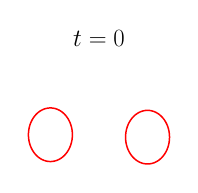
\begin{tikzpicture}[scale=0.36]

\begin{axis}[
  xmin = -6,
  xmax = 2,
  ymin = -2,
  ymax = 2,
  axis equal = true,
  hide axis,
  title = {\Huge$t=0$}
  ]

\addplot [mark=none,red,line width=1.5] table{
-4.0000e+00 1.2044e+00
-4.0888e+00 1.1991e+00
-4.1766e+00 1.1832e+00
-4.2628e+00 1.1568e+00
-4.3465e+00 1.1203e+00
-4.4268e+00 1.0740e+00
-4.5031e+00 1.0183e+00
-4.5744e+00 9.5370e-01
-4.6403e+00 8.8092e-01
-4.6999e+00 8.0062e-01
-4.7529e+00 7.1357e-01
-4.7986e+00 6.2061e-01
-4.8366e+00 5.2263e-01
-4.8665e+00 4.2059e-01
-4.8881e+00 3.1546e-01
-4.9011e+00 2.0825e-01
-4.9055e+00 1.0000e-01
-4.9011e+00 -8.2491e-03
-4.8881e+00 -1.1546e-01
-4.8665e+00 -2.2059e-01
-4.8366e+00 -3.2263e-01
-4.7986e+00 -4.2061e-01
-4.7529e+00 -5.1357e-01
-4.6999e+00 -6.0062e-01
-4.6403e+00 -6.8092e-01
-4.5744e+00 -7.5370e-01
-4.5031e+00 -8.1827e-01
-4.4268e+00 -8.7398e-01
-4.3465e+00 -9.2032e-01
-4.2628e+00 -9.5683e-01
-4.1766e+00 -9.8317e-01
-4.0888e+00 -9.9907e-01
-4.0000e+00 -1.0044e+00
-3.9112e+00 -9.9907e-01
-3.8234e+00 -9.8317e-01
-3.7372e+00 -9.5683e-01
-3.6535e+00 -9.2032e-01
-3.5732e+00 -8.7398e-01
-3.4969e+00 -8.1827e-01
-3.4256e+00 -7.5370e-01
-3.3597e+00 -6.8092e-01
-3.3001e+00 -6.0062e-01
-3.2471e+00 -5.1357e-01
-3.2014e+00 -4.2061e-01
-3.1634e+00 -3.2263e-01
-3.1335e+00 -2.2059e-01
-3.1119e+00 -1.1546e-01
-3.0989e+00 -8.2491e-03
-3.0945e+00 1.0000e-01
-3.0989e+00 2.0825e-01
-3.1119e+00 3.1546e-01
-3.1335e+00 4.2059e-01
-3.1634e+00 5.2263e-01
-3.2014e+00 6.2061e-01
-3.2471e+00 7.1357e-01
-3.3001e+00 8.0062e-01
-3.3597e+00 8.8092e-01
-3.4256e+00 9.5370e-01
-3.4969e+00 1.0183e+00
-3.5732e+00 1.0740e+00
-3.6535e+00 1.1203e+00
-3.7372e+00 1.1568e+00
-3.8234e+00 1.1832e+00
-3.9112e+00 1.1991e+00
-4.0000e+00 1.2044e+00
};

\addplot [mark=none,red,line width=1.5] table{
6.7624e-17 1.1044e+00
-8.8752e-02 1.0991e+00
-1.7665e-01 1.0832e+00
-2.6285e-01 1.0568e+00
-3.4651e-01 1.0203e+00
-4.2684e-01 9.7398e-01
-5.0306e-01 9.1827e-01
-5.7443e-01 8.5370e-01
-6.4027e-01 7.8092e-01
-6.9994e-01 7.0062e-01
-7.5288e-01 6.1357e-01
-7.9856e-01 5.2061e-01
-8.3655e-01 4.2263e-01
-8.6649e-01 3.2059e-01
-8.8808e-01 2.1546e-01
-9.0112e-01 1.0825e-01
-9.0548e-01 1.2307e-16
-9.0112e-01 -1.0825e-01
-8.8808e-01 -2.1546e-01
-8.6649e-01 -3.2059e-01
-8.3655e-01 -4.2263e-01
-7.9856e-01 -5.2061e-01
-7.5288e-01 -6.1357e-01
-6.9994e-01 -7.0062e-01
-6.4027e-01 -7.8092e-01
-5.7443e-01 -8.5370e-01
-5.0306e-01 -9.1827e-01
-4.2684e-01 -9.7398e-01
-3.4651e-01 -1.0203e+00
-2.6285e-01 -1.0568e+00
-1.7665e-01 -1.0832e+00
-8.8752e-02 -1.0991e+00
-1.7851e-16 -1.1044e+00
8.8752e-02 -1.0991e+00
1.7665e-01 -1.0832e+00
2.6285e-01 -1.0568e+00
3.4651e-01 -1.0203e+00
4.2684e-01 -9.7398e-01
5.0306e-01 -9.1827e-01
5.7443e-01 -8.5370e-01
6.4027e-01 -7.8092e-01
6.9994e-01 -7.0062e-01
7.5288e-01 -6.1357e-01
7.9856e-01 -5.2061e-01
8.3655e-01 -4.2263e-01
8.6649e-01 -3.2059e-01
8.8808e-01 -2.1546e-01
9.0112e-01 -1.0825e-01
9.0548e-01 -2.5832e-16
9.0112e-01 1.0825e-01
8.8808e-01 2.1546e-01
8.6649e-01 3.2059e-01
8.3655e-01 4.2263e-01
7.9856e-01 5.2061e-01
7.5288e-01 6.1357e-01
6.9994e-01 7.0062e-01
6.4027e-01 7.8092e-01
5.7443e-01 8.5370e-01
5.0306e-01 9.1827e-01
4.2684e-01 9.7398e-01
3.4651e-01 1.0203e+00
2.6285e-01 1.0568e+00
1.7665e-01 1.0832e+00
8.8752e-02 1.0991e+00
6.7624e-17 1.1044e+00
};

\end{axis}
\end{tikzpicture}

 &
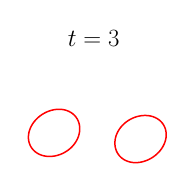
\begin{tikzpicture}[scale=0.36]

\begin{axis}[
  xmin = -6,
  xmax = 2,
  ymin = -2,
  ymax = 2,
  axis equal = true,
  hide axis,
  title = {\Huge$t=3$}
  ]

\addplot [mark=none,red,line width=1.5] table{
-2.5859e+00 4.9427e-01
-2.6062e+00 5.8147e-01
-2.6363e+00 6.6622e-01
-2.6764e+00 7.4760e-01
-2.7267e+00 8.2453e-01
-2.7870e+00 8.9578e-01
-2.8569e+00 9.6008e-01
-2.9357e+00 1.0163e+00
-3.0225e+00 1.0633e+00
-3.1160e+00 1.1004e+00
-3.2149e+00 1.1272e+00
-3.3178e+00 1.1434e+00
-3.4234e+00 1.1490e+00
-3.5302e+00 1.1443e+00
-3.6371e+00 1.1296e+00
-3.7430e+00 1.1055e+00
-3.8468e+00 1.0724e+00
-3.9475e+00 1.0309e+00
-4.0443e+00 9.8168e-01
-4.1364e+00 9.2543e-01
-4.2231e+00 8.6281e-01
-4.3037e+00 7.9452e-01
-4.3778e+00 7.2126e-01
-4.4447e+00 6.4372e-01
-4.5042e+00 5.6257e-01
-4.5558e+00 4.7845e-01
-4.5993e+00 3.9197e-01
-4.6344e+00 3.0372e-01
-4.6609e+00 2.1424e-01
-4.6786e+00 1.2407e-01
-4.6870e+00 3.3740e-02
-4.6861e+00 -5.6184e-02
-4.6755e+00 -1.4507e-01
-4.6549e+00 -2.3219e-01
-4.6241e+00 -3.1667e-01
-4.5830e+00 -3.9753e-01
-4.5316e+00 -4.7366e-01
-4.4701e+00 -5.4390e-01
-4.3992e+00 -6.0711e-01
-4.3196e+00 -6.6224e-01
-4.2324e+00 -7.0844e-01
-4.1387e+00 -7.4507e-01
-4.0397e+00 -7.7172e-01
-3.9369e+00 -7.8820e-01
-3.8314e+00 -7.9451e-01
-3.7245e+00 -7.9079e-01
-3.6174e+00 -7.7733e-01
-3.5113e+00 -7.5448e-01
-3.4071e+00 -7.2268e-01
-3.3058e+00 -6.8243e-01
-3.2085e+00 -6.3429e-01
-3.1159e+00 -5.7885e-01
-3.0288e+00 -5.1677e-01
-2.9480e+00 -4.4871e-01
-2.8741e+00 -3.7538e-01
-2.8075e+00 -2.9751e-01
-2.7488e+00 -2.1583e-01
-2.6982e+00 -1.3110e-01
-2.6560e+00 -4.3996e-02
-2.6223e+00 4.4800e-02
-2.5973e+00 1.3468e-01
-2.5810e+00 2.2509e-01
-2.5736e+00 3.1550e-01
-2.5751e+00 4.0541e-01
-2.5859e+00 4.9427e-01
};

\addplot [mark=none,red,line width=1.5] table{
9.7550e-01 2.4507e-01
9.5491e-01 3.3219e-01
9.2410e-01 4.1667e-01
8.8297e-01 4.9753e-01
8.3155e-01 5.7366e-01
7.7012e-01 6.4390e-01
6.9922e-01 7.0711e-01
6.1964e-01 7.6224e-01
5.3240e-01 8.0844e-01
4.3868e-01 8.4507e-01
3.3974e-01 8.7172e-01
2.3689e-01 8.8820e-01
1.3140e-01 8.9451e-01
2.4514e-02 8.9079e-01
-8.2575e-02 8.7733e-01
-1.8875e-01 8.5448e-01
-2.9295e-01 8.2268e-01
-3.9418e-01 7.8243e-01
-4.9152e-01 7.3429e-01
-5.8412e-01 6.7885e-01
-6.7117e-01 6.1677e-01
-7.5198e-01 5.4871e-01
-8.2593e-01 4.7538e-01
-8.9248e-01 3.9751e-01
-9.5122e-01 3.1583e-01
-1.0018e+00 2.3110e-01
-1.0440e+00 1.4400e-01
-1.0777e+00 5.5200e-02
-1.1027e+00 -3.4680e-02
-1.1190e+00 -1.2509e-01
-1.1264e+00 -2.1550e-01
-1.1249e+00 -3.0541e-01
-1.1141e+00 -3.9427e-01
-1.0938e+00 -4.8147e-01
-1.0637e+00 -5.6622e-01
-1.0236e+00 -6.4760e-01
-9.7331e-01 -7.2453e-01
-9.1303e-01 -7.9578e-01
-8.4311e-01 -8.6008e-01
-7.6426e-01 -9.1627e-01
-6.7747e-01 -9.6331e-01
-5.8396e-01 -1.0004e+00
-4.8505e-01 -1.0272e+00
-3.8216e-01 -1.0434e+00
-2.7664e-01 -1.0490e+00
-1.6980e-01 -1.0443e+00
-6.2876e-02 -1.0296e+00
4.3002e-02 -1.0055e+00
1.4679e-01 -9.7236e-01
2.4752e-01 -9.3088e-01
3.4434e-01 -8.8168e-01
4.3644e-01 -8.2543e-01
5.2311e-01 -7.6281e-01
6.0374e-01 -6.9452e-01
6.7777e-01 -6.2126e-01
7.4472e-01 -5.4372e-01
8.0418e-01 -4.6257e-01
8.5582e-01 -3.7845e-01
8.9933e-01 -2.9197e-01
9.3445e-01 -2.0372e-01
9.6094e-01 -1.1424e-01
9.7855e-01 -2.4072e-02
9.8704e-01 6.6260e-02
9.8611e-01 1.5618e-01
9.7550e-01 2.4507e-01
};

\end{axis}
\end{tikzpicture}

 &
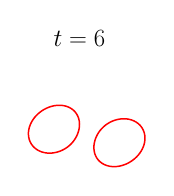
\begin{tikzpicture}[scale=0.36]

\begin{axis}[
  xmin = -6,
  xmax = 2,
  ymin = -2,
  ymax = 2,
  axis equal = true,
  hide axis,
  title = {\Huge$t=6$}
  ]

\addplot [mark=none,red,line width=1.5] table{
-2.4503e+00 -3.7535e-01
-2.3824e+00 -3.1632e-01
-2.3187e+00 -2.5231e-01
-2.2591e+00 -1.8323e-01
-2.2040e+00 -1.0904e-01
-2.1538e+00 -2.9703e-02
-2.1090e+00 5.4749e-02
-2.0703e+00 1.4419e-01
-2.0385e+00 2.3837e-01
-2.0146e+00 3.3686e-01
-2.0000e+00 4.3902e-01
-1.9961e+00 5.4384e-01
-2.0044e+00 6.4991e-01
-2.0262e+00 7.5529e-01
-2.0626e+00 8.5759e-01
-2.1137e+00 9.5407e-01
-2.1788e+00 1.0420e+00
-2.2565e+00 1.1190e+00
-2.3444e+00 1.1834e+00
-2.4399e+00 1.2345e+00
-2.5402e+00 1.2723e+00
-2.6432e+00 1.2974e+00
-2.7467e+00 1.3109e+00
-2.8494e+00 1.3138e+00
-2.9500e+00 1.3073e+00
-3.0479e+00 1.2925e+00
-3.1424e+00 1.2705e+00
-3.2333e+00 1.2420e+00
-3.3204e+00 1.2078e+00
-3.4037e+00 1.1684e+00
-3.4833e+00 1.1241e+00
-3.5592e+00 1.0752e+00
-3.6315e+00 1.0218e+00
-3.7002e+00 9.6380e-01
-3.7653e+00 9.0113e-01
-3.8267e+00 8.3361e-01
-3.8839e+00 7.6103e-01
-3.9364e+00 6.8322e-01
-3.9836e+00 6.0006e-01
-4.0245e+00 5.1156e-01
-4.0580e+00 4.1793e-01
-4.0826e+00 3.1963e-01
-4.0970e+00 2.1746e-01
-4.0997e+00 1.1262e-01
-4.0892e+00 6.7733e-03
-4.0646e+00 -9.7962e-02
-4.0254e+00 -1.9913e-01
-3.9717e+00 -2.9415e-01
-3.9046e+00 -3.8059e-01
-3.8258e+00 -4.5645e-01
-3.7375e+00 -5.2040e-01
-3.6423e+00 -5.7180e-01
-3.5423e+00 -6.1066e-01
-3.4398e+00 -6.3746e-01
-3.3365e+00 -6.5297e-01
-3.2339e+00 -6.5814e-01
-3.1331e+00 -6.5396e-01
-3.0350e+00 -6.4137e-01
-2.9400e+00 -6.2125e-01
-2.8487e+00 -5.9435e-01
-2.7611e+00 -5.6129e-01
-2.6775e+00 -5.2257e-01
-2.5978e+00 -4.7854e-01
-2.5221e+00 -4.2943e-01
-2.4503e+00 -3.7535e-01
};

\addplot [mark=none,red,line width=1.5] table{
2.3145e-01 -9.2179e-01
3.0019e-01 -8.6380e-01
3.6531e-01 -8.0113e-01
4.2665e-01 -7.3361e-01
4.8387e-01 -6.6103e-01
5.3644e-01 -5.8322e-01
5.8364e-01 -5.0006e-01
6.2454e-01 -4.1156e-01
6.5798e-01 -3.1793e-01
6.8263e-01 -2.1963e-01
6.9703e-01 -1.1746e-01
6.9968e-01 -1.2618e-02
6.8923e-01 9.3227e-02
6.6462e-01 1.9796e-01
6.2536e-01 2.9913e-01
5.7166e-01 3.9415e-01
5.0456e-01 4.8059e-01
4.2578e-01 5.5645e-01
3.3753e-01 6.2040e-01
2.4225e-01 6.7180e-01
1.4229e-01 7.1066e-01
3.9781e-02 7.3746e-01
-6.3488e-02 7.5297e-01
-1.6607e-01 7.5814e-01
-2.6685e-01 7.5396e-01
-3.6501e-01 7.4137e-01
-4.5997e-01 7.2125e-01
-5.5134e-01 6.9435e-01
-6.3889e-01 6.6129e-01
-7.2253e-01 6.2257e-01
-8.0221e-01 5.7854e-01
-8.7794e-01 5.2943e-01
-9.4973e-01 4.7535e-01
-1.0176e+00 4.1632e-01
-1.0813e+00 3.5231e-01
-1.1409e+00 2.8323e-01
-1.1960e+00 2.0904e-01
-1.2462e+00 1.2970e-01
-1.2910e+00 4.5251e-02
-1.3297e+00 -4.4188e-02
-1.3615e+00 -1.3837e-01
-1.3854e+00 -2.3686e-01
-1.4000e+00 -3.3902e-01
-1.4039e+00 -4.4384e-01
-1.3956e+00 -5.4991e-01
-1.3738e+00 -6.5529e-01
-1.3374e+00 -7.5759e-01
-1.2863e+00 -8.5407e-01
-1.2212e+00 -9.4198e-01
-1.1435e+00 -1.0190e+00
-1.0556e+00 -1.0834e+00
-9.6012e-01 -1.1345e+00
-8.5976e-01 -1.1723e+00
-7.5684e-01 -1.1974e+00
-6.5329e-01 -1.2109e+00
-5.5063e-01 -1.2138e+00
-4.4998e-01 -1.2073e+00
-3.5213e-01 -1.1925e+00
-2.5760e-01 -1.1705e+00
-1.6671e-01 -1.1420e+00
-7.9592e-02 -1.1078e+00
3.7182e-03 -1.0684e+00
8.3273e-02 -1.0241e+00
1.5916e-01 -9.7522e-01
2.3145e-01 -9.2179e-01
};

\end{axis}
\end{tikzpicture}

 &
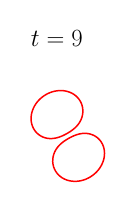
\begin{tikzpicture}[scale=0.36]

\begin{axis}[
  xmin = -6,
  xmax = 2,
  ymin = -2,
  ymax = 2,
  axis equal = true,
  hide axis,
  title = {\Huge$t=9$}
  ]

\addplot [mark=none,red,line width=1.5] table{
-2.5643e+00 1.7159e-03
-2.4789e+00 -2.7230e-02
-2.3903e+00 -4.6672e-02
-2.2994e+00 -5.6578e-02
-2.2067e+00 -5.6981e-02
-2.1130e+00 -4.8038e-02
-2.0188e+00 -3.0102e-02
-1.9247e+00 -3.7772e-03
-1.8309e+00 3.0086e-02
-1.7376e+00 7.0498e-02
-1.6448e+00 1.1655e-01
-1.5527e+00 1.6765e-01
-1.4618e+00 2.2374e-01
-1.3728e+00 2.8527e-01
-1.2872e+00 3.5308e-01
-1.2068e+00 4.2796e-01
-1.1336e+00 5.1031e-01
-1.0695e+00 5.9991e-01
-1.0162e+00 6.9589e-01
-9.7496e-01 7.9685e-01
-9.4660e-01 9.0109e-01
-9.3150e-01 1.0067e+00
-9.2964e-01 1.1119e+00
-9.4068e-01 1.2147e+00
-9.6395e-01 1.3135e+00
-9.9852e-01 1.4069e+00
-1.0433e+00 1.4936e+00
-1.0970e+00 1.5729e+00
-1.1584e+00 1.6442e+00
-1.2263e+00 1.7071e+00
-1.2997e+00 1.7617e+00
-1.3777e+00 1.8080e+00
-1.4595e+00 1.8460e+00
-1.5446e+00 1.8761e+00
-1.6326e+00 1.8982e+00
-1.7230e+00 1.9125e+00
-1.8155e+00 1.9190e+00
-1.9097e+00 1.9175e+00
-2.0051e+00 1.9080e+00
-2.1013e+00 1.8903e+00
-2.1976e+00 1.8643e+00
-2.2933e+00 1.8300e+00
-2.3877e+00 1.7872e+00
-2.4797e+00 1.7360e+00
-2.5685e+00 1.6766e+00
-2.6531e+00 1.6093e+00
-2.7324e+00 1.5344e+00
-2.8054e+00 1.4524e+00
-2.8710e+00 1.3640e+00
-2.9284e+00 1.2700e+00
-2.9765e+00 1.1714e+00
-3.0145e+00 1.0692e+00
-3.0418e+00 9.6469e-01
-3.0579e+00 8.5918e-01
-3.0624e+00 7.5409e-01
-3.0552e+00 6.5090e-01
-3.0366e+00 5.5107e-01
-3.0070e+00 4.5596e-01
-2.9671e+00 3.6682e-01
-2.9177e+00 2.8471e-01
-2.8599e+00 2.1046e-01
-2.7947e+00 1.4468e-01
-2.7231e+00 8.7806e-02
-2.6460e+00 4.0096e-02
-2.5643e+00 1.7159e-03
};

\addplot [mark=none,red,line width=1.5] table{
-1.6405e+00 -1.7460e+00
-1.5554e+00 -1.7761e+00
-1.4674e+00 -1.7982e+00
-1.3770e+00 -1.8125e+00
-1.2845e+00 -1.8190e+00
-1.1903e+00 -1.8175e+00
-1.0949e+00 -1.8080e+00
-9.9867e-01 -1.7903e+00
-9.0237e-01 -1.7643e+00
-8.0666e-01 -1.7300e+00
-7.1234e-01 -1.6872e+00
-6.2031e-01 -1.6360e+00
-5.3151e-01 -1.5766e+00
-4.4694e-01 -1.5093e+00
-3.6763e-01 -1.4344e+00
-2.9463e-01 -1.3524e+00
-2.2896e-01 -1.2640e+00
-1.7161e-01 -1.1700e+00
-1.2350e-01 -1.0714e+00
-8.5451e-02 -9.6921e-01
-5.8151e-02 -8.6469e-01
-4.2114e-02 -7.5918e-01
-3.7647e-02 -6.5409e-01
-4.4816e-02 -5.5090e-01
-6.3429e-02 -4.5107e-01
-9.3035e-02 -3.5596e-01
-1.3295e-01 -2.6682e-01
-1.8230e-01 -1.8471e-01
-2.4010e-01 -1.1046e-01
-3.0532e-01 -4.4683e-02
-3.7694e-01 1.2194e-02
-4.5401e-01 5.9904e-02
-5.3567e-01 9.8284e-02
-6.2114e-01 1.2723e-01
-7.0970e-01 1.4667e-01
-8.0064e-01 1.5658e-01
-8.9331e-01 1.5698e-01
-9.8703e-01 1.4804e-01
-1.0812e+00 1.3010e-01
-1.1753e+00 1.0378e-01
-1.2691e+00 6.9914e-02
-1.3624e+00 2.9502e-02
-1.4552e+00 -1.6548e-02
-1.5473e+00 -6.7650e-02
-1.6382e+00 -1.2374e-01
-1.7272e+00 -1.8527e-01
-1.8128e+00 -2.5308e-01
-1.8932e+00 -3.2796e-01
-1.9664e+00 -4.1031e-01
-2.0305e+00 -4.9991e-01
-2.0838e+00 -5.9589e-01
-2.1250e+00 -6.9685e-01
-2.1534e+00 -8.0109e-01
-2.1685e+00 -9.0673e-01
-2.1704e+00 -1.0119e+00
-2.1593e+00 -1.1147e+00
-2.1361e+00 -1.2135e+00
-2.1015e+00 -1.3069e+00
-2.0567e+00 -1.3936e+00
-2.0030e+00 -1.4729e+00
-1.9416e+00 -1.5442e+00
-1.8737e+00 -1.6071e+00
-1.8003e+00 -1.6617e+00
-1.7223e+00 -1.7080e+00
-1.6405e+00 -1.7460e+00
};

\end{axis}
\end{tikzpicture}

 &
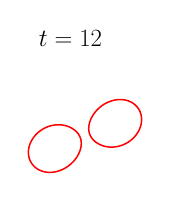
\begin{tikzpicture}[scale=0.36]

\begin{axis}[
  xmin = -6,
  xmax = 2,
  ymin = -2,
  ymax = 2,
  axis equal = true,
  hide axis,
  title = {\Huge$t=12$}
  ]

\addplot [mark=none,red,line width=1.5] table{
-1.0356e+00 9.6029e-01
-1.0855e+00 8.8378e-01
-1.1302e+00 8.0356e-01
-1.1692e+00 7.1946e-01
-1.2017e+00 6.3137e-01
-1.2267e+00 5.3928e-01
-1.2426e+00 4.4347e-01
-1.2474e+00 3.4464e-01
-1.2389e+00 2.4422e-01
-1.2150e+00 1.4442e-01
-1.1747e+00 4.8116e-02
-1.1186e+00 -4.1903e-02
-1.0487e+00 -1.2356e-01
-9.6728e-01 -1.9573e-01
-8.7677e-01 -2.5783e-01
-7.7921e-01 -3.0956e-01
-6.7637e-01 -3.5066e-01
-5.6988e-01 -3.8104e-01
-4.6127e-01 -4.0070e-01
-3.5196e-01 -4.0987e-01
-2.4328e-01 -4.0892e-01
-1.3638e-01 -3.9844e-01
-3.2259e-02 -3.7910e-01
6.8249e-02 -3.5164e-01
1.6451e-01 -3.1684e-01
2.5603e-01 -2.7544e-01
3.4250e-01 -2.2814e-01
4.2368e-01 -1.7555e-01
4.9947e-01 -1.1816e-01
5.6980e-01 -5.6370e-02
6.3467e-01 9.5559e-03
6.9400e-01 7.9454e-02
7.4772e-01 1.5328e-01
7.9561e-01 2.3102e-01
8.3735e-01 3.1274e-01
8.7242e-01 3.9842e-01
9.0015e-01 4.8799e-01
9.1965e-01 5.8122e-01
9.2990e-01 6.7763e-01
9.2976e-01 7.7643e-01
9.1811e-01 8.7647e-01
8.9391e-01 9.7620e-01
8.5646e-01 1.0737e+00
8.0553e-01 1.1668e+00
7.4145e-01 1.2532e+00
6.6519e-01 1.3309e+00
5.7831e-01 1.3980e+00
4.8273e-01 1.4533e+00
3.8062e-01 1.4961e+00
2.7411e-01 1.5263e+00
1.6522e-01 1.5442e+00
5.5735e-02 1.5504e+00
-5.2825e-02 1.5458e+00
-1.5923e-01 1.5313e+00
-2.6247e-01 1.5079e+00
-3.6181e-01 1.4765e+00
-4.5669e-01 1.4382e+00
-5.4675e-01 1.3939e+00
-6.3178e-01 1.3441e+00
-7.1167e-01 1.2897e+00
-7.8644e-01 1.2311e+00
-8.5614e-01 1.1687e+00
-9.2086e-01 1.1027e+00
-9.8067e-01 1.0332e+00
-1.0356e+00 9.6029e-01
};

\addplot [mark=none,red,line width=1.5] table{
-3.5477e+00 -5.3277e-02
-3.5956e+00 -1.3102e-01
-3.6373e+00 -2.1274e-01
-3.6724e+00 -2.9842e-01
-3.7001e+00 -3.8799e-01
-3.7196e+00 -4.8122e-01
-3.7299e+00 -5.7763e-01
-3.7298e+00 -6.7643e-01
-3.7181e+00 -7.7647e-01
-3.6939e+00 -8.7620e-01
-3.6565e+00 -9.7371e-01
-3.6055e+00 -1.0668e+00
-3.5414e+00 -1.1532e+00
-3.4652e+00 -1.2309e+00
-3.3783e+00 -1.2980e+00
-3.2827e+00 -1.3533e+00
-3.1806e+00 -1.3961e+00
-3.0741e+00 -1.4263e+00
-2.9652e+00 -1.4442e+00
-2.8557e+00 -1.4504e+00
-2.7472e+00 -1.4458e+00
-2.6408e+00 -1.4313e+00
-2.5375e+00 -1.4079e+00
-2.4382e+00 -1.3765e+00
-2.3433e+00 -1.3382e+00
-2.2532e+00 -1.2939e+00
-2.1682e+00 -1.2441e+00
-2.0883e+00 -1.1897e+00
-2.0136e+00 -1.1311e+00
-1.9439e+00 -1.0687e+00
-1.8791e+00 -1.0027e+00
-1.8193e+00 -9.3322e-01
-1.7644e+00 -8.6029e-01
-1.7145e+00 -7.8378e-01
-1.6698e+00 -7.0356e-01
-1.6308e+00 -6.1946e-01
-1.5983e+00 -5.3137e-01
-1.5733e+00 -4.3928e-01
-1.5574e+00 -3.4347e-01
-1.5526e+00 -2.4464e-01
-1.5611e+00 -1.4422e-01
-1.5850e+00 -4.4423e-02
-1.6253e+00 5.1884e-02
-1.6814e+00 1.4190e-01
-1.7513e+00 2.2356e-01
-1.8327e+00 2.9573e-01
-1.9232e+00 3.5783e-01
-2.0208e+00 4.0956e-01
-2.1236e+00 4.5066e-01
-2.2301e+00 4.8104e-01
-2.3387e+00 5.0070e-01
-2.4480e+00 5.0987e-01
-2.5567e+00 5.0892e-01
-2.6636e+00 4.9844e-01
-2.7677e+00 4.7910e-01
-2.8682e+00 4.5164e-01
-2.9645e+00 4.1684e-01
-3.0560e+00 3.7544e-01
-3.1425e+00 3.2814e-01
-3.2237e+00 2.7555e-01
-3.2995e+00 2.1816e-01
-3.3698e+00 1.5637e-01
-3.4347e+00 9.0444e-02
-3.4940e+00 2.0546e-02
-3.5477e+00 -5.3277e-02
};

\end{axis}
\end{tikzpicture}


\fi
\end{tabular}
\begin{tabular}{cc}
\ifInputs
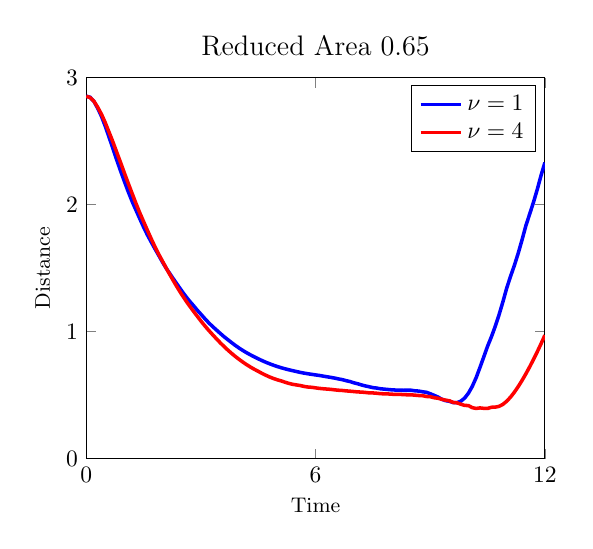
\begin{tikzpicture}[scale=0.85]

\begin{axis}[
  xmin = 0,
  xmax = 12, 
  ymin = 0,
  ymax = 3,
  xtick = {0,6,12,18,24},
  xticklabels = {$0$,$6$,$12$,$18$,$24$},
  ytick = {0,1,2,3},
  yticklabels = {$0$,$1$,$2$,$3$},
  xlabel = {Time},
  ylabel = {Distance},
  label style = {font=\small},
  legend entries = {$\nu=1$,$\nu=4$},
  title = {\large{Reduced Area 0.65}}
  ]

\addplot [mark=none,blue,line width=1.5] table{
0.0000e+00 2.8531e+00
1.0000e-01 2.8450e+00
2.0000e-01 2.8130e+00
3.0000e-01 2.7588e+00
4.0000e-01 2.6942e+00
5.0000e-01 2.6158e+00
6.0000e-01 2.5286e+00
7.0000e-01 2.4404e+00
8.0000e-01 2.3502e+00
9.0000e-01 2.2643e+00
1.0000e+00 2.1815e+00
1.1000e+00 2.1009e+00
1.2000e+00 2.0258e+00
1.3000e+00 1.9573e+00
1.4000e+00 1.8897e+00
1.5000e+00 1.8236e+00
1.6000e+00 1.7618e+00
1.7000e+00 1.7057e+00
1.8000e+00 1.6511e+00
1.9000e+00 1.5987e+00
2.0000e+00 1.5448e+00
2.1000e+00 1.4954e+00
2.2000e+00 1.4504e+00
2.3000e+00 1.4064e+00
2.4000e+00 1.3633e+00
2.5000e+00 1.3202e+00
2.6000e+00 1.2790e+00
2.7000e+00 1.2412e+00
2.8000e+00 1.2068e+00
2.9000e+00 1.1704e+00
3.0000e+00 1.1371e+00
3.1000e+00 1.1031e+00
3.2000e+00 1.0710e+00
3.3000e+00 1.0415e+00
3.4000e+00 1.0145e+00
3.5000e+00 9.8739e-01
3.6000e+00 9.6133e-01
3.7000e+00 9.3737e-01
3.8000e+00 9.1418e-01
3.9000e+00 8.9130e-01
4.0000e+00 8.7022e-01
4.1000e+00 8.5077e-01
4.2000e+00 8.3282e-01
4.3000e+00 8.1622e-01
4.4000e+00 8.0084e-01
4.5000e+00 7.8585e-01
4.6000e+00 7.7159e-01
4.7000e+00 7.5845e-01
4.8000e+00 7.4634e-01
4.9000e+00 7.3520e-01
5.0000e+00 7.2496e-01
5.1000e+00 7.1559e-01
5.2000e+00 7.0706e-01
5.3000e+00 6.9938e-01
5.4000e+00 6.9246e-01
5.5000e+00 6.8553e-01
5.6000e+00 6.7890e-01
5.7000e+00 6.7299e-01
5.8000e+00 6.6790e-01
5.9000e+00 6.6341e-01
6.0000e+00 6.5881e-01
6.1000e+00 6.5449e-01
6.2000e+00 6.4944e-01
6.3000e+00 6.4415e-01
6.4000e+00 6.3916e-01
6.5000e+00 6.3382e-01
6.6000e+00 6.2731e-01
6.7000e+00 6.2176e-01
6.8000e+00 6.1347e-01
6.9000e+00 6.0690e-01
7.0000e+00 5.9685e-01
7.1000e+00 5.8949e-01
7.2000e+00 5.8011e-01
7.3000e+00 5.7244e-01
7.4000e+00 5.6590e-01
7.5000e+00 5.5863e-01
7.6000e+00 5.5544e-01
7.7000e+00 5.4959e-01
7.8000e+00 5.4687e-01
7.9000e+00 5.4405e-01
8.0000e+00 5.4138e-01
8.1000e+00 5.3964e-01
8.2000e+00 5.3852e-01
8.3000e+00 5.3803e-01
8.4000e+00 5.3819e-01
8.5000e+00 5.3816e-01
8.6000e+00 5.3370e-01
8.7000e+00 5.3159e-01
8.8000e+00 5.2603e-01
8.9000e+00 5.2205e-01
9.0000e+00 5.1079e-01
9.1000e+00 4.9818e-01
9.2000e+00 4.8514e-01
9.3000e+00 4.6758e-01
9.4000e+00 4.5670e-01
9.5000e+00 4.5139e-01
9.6000e+00 4.4093e-01
9.7000e+00 4.4051e-01
9.8000e+00 4.5179e-01
9.9000e+00 4.7630e-01
1.0000e+01 5.1515e-01
1.0100e+01 5.6864e-01
1.0200e+01 6.3619e-01
1.0300e+01 7.1663e-01
1.0400e+01 8.0004e-01
1.0500e+01 8.8447e-01
1.0600e+01 9.5850e-01
1.0700e+01 1.0405e+00
1.0800e+01 1.1320e+00
1.0900e+01 1.2330e+00
1.1000e+01 1.3416e+00
1.1100e+01 1.4339e+00
1.1200e+01 1.5199e+00
1.1300e+01 1.6153e+00
1.1400e+01 1.7201e+00
1.1500e+01 1.8316e+00
1.1600e+01 1.9242e+00
1.1700e+01 2.0169e+00
1.1800e+01 2.1190e+00
1.1900e+01 2.2301e+00
1.2000e+01 2.3305e+00
};

\addplot [mark=none,red,line width=1.5] table{
0.0000e+00 2.8531e+00
1.0000e-01 2.8425e+00
2.0000e-01 2.8141e+00
3.0000e-01 2.7663e+00
4.0000e-01 2.7108e+00
5.0000e-01 2.6437e+00
6.0000e-01 2.5684e+00
7.0000e-01 2.4921e+00
8.0000e-01 2.4106e+00
9.0000e-01 2.3303e+00
1.0000e+00 2.2477e+00
1.1000e+00 2.1671e+00
1.2000e+00 2.0883e+00
1.3000e+00 2.0102e+00
1.4000e+00 1.9360e+00
1.5000e+00 1.8667e+00
1.6000e+00 1.7981e+00
1.7000e+00 1.7310e+00
1.8000e+00 1.6668e+00
1.9000e+00 1.6071e+00
2.0000e+00 1.5516e+00
2.1000e+00 1.4956e+00
2.2000e+00 1.4425e+00
2.3000e+00 1.3902e+00
2.4000e+00 1.3394e+00
2.5000e+00 1.2914e+00
2.6000e+00 1.2462e+00
2.7000e+00 1.2034e+00
2.8000e+00 1.1629e+00
2.9000e+00 1.1230e+00
3.0000e+00 1.0838e+00
3.1000e+00 1.0467e+00
3.2000e+00 1.0115e+00
3.3000e+00 9.7804e-01
3.4000e+00 9.4557e-01
3.5000e+00 9.1400e-01
3.6000e+00 8.8418e-01
3.7000e+00 8.5605e-01
3.8000e+00 8.2954e-01
3.9000e+00 8.0461e-01
4.0000e+00 7.8123e-01
4.1000e+00 7.5938e-01
4.2000e+00 7.3905e-01
4.3000e+00 7.2026e-01
4.4000e+00 7.0303e-01
4.5000e+00 6.8709e-01
4.6000e+00 6.7088e-01
4.7000e+00 6.5600e-01
4.8000e+00 6.4254e-01
4.9000e+00 6.3061e-01
5.0000e+00 6.2035e-01
5.1000e+00 6.1191e-01
5.2000e+00 6.0149e-01
5.3000e+00 5.9231e-01
5.4000e+00 5.8509e-01
5.5000e+00 5.8006e-01
5.6000e+00 5.7532e-01
5.7000e+00 5.6822e-01
5.8000e+00 5.6362e-01
5.9000e+00 5.6131e-01
6.0000e+00 5.5688e-01
6.1000e+00 5.5282e-01
6.2000e+00 5.4992e-01
6.3000e+00 5.4744e-01
6.4000e+00 5.4511e-01
6.5000e+00 5.4129e-01
6.6000e+00 5.3829e-01
6.7000e+00 5.3633e-01
6.8000e+00 5.3323e-01
6.9000e+00 5.3073e-01
7.0000e+00 5.2811e-01
7.1000e+00 5.2498e-01
7.2000e+00 5.2383e-01
7.3000e+00 5.2099e-01
7.4000e+00 5.1770e-01
7.5000e+00 5.1693e-01
7.6000e+00 5.1455e-01
7.7000e+00 5.1113e-01
7.8000e+00 5.1003e-01
7.9000e+00 5.0897e-01
8.0000e+00 5.0693e-01
8.1000e+00 5.0519e-01
8.2000e+00 5.0612e-01
8.3000e+00 5.0335e-01
8.4000e+00 5.0253e-01
8.5000e+00 5.0236e-01
8.6000e+00 4.9943e-01
8.7000e+00 4.9680e-01
8.8000e+00 4.9512e-01
8.9000e+00 4.8914e-01
9.0000e+00 4.8753e-01
9.1000e+00 4.7934e-01
9.2000e+00 4.7539e-01
9.3000e+00 4.6720e-01
9.4000e+00 4.6023e-01
9.5000e+00 4.5526e-01
9.6000e+00 4.4234e-01
9.7000e+00 4.3923e-01
9.8000e+00 4.2839e-01
9.9000e+00 4.1876e-01
1.0000e+01 4.1755e-01
1.0100e+01 4.0116e-01
1.0200e+01 3.9493e-01
1.0300e+01 3.9913e-01
1.0400e+01 3.9578e-01
1.0500e+01 3.9483e-01
1.0600e+01 4.0415e-01
1.0700e+01 4.0543e-01
1.0800e+01 4.1119e-01
1.0900e+01 4.2691e-01
1.1000e+01 4.5154e-01
1.1100e+01 4.8379e-01
1.1200e+01 5.2237e-01
1.1300e+01 5.6617e-01
1.1400e+01 6.1434e-01
1.1500e+01 6.6627e-01
1.1600e+01 7.2153e-01
1.1700e+01 7.7985e-01
1.1800e+01 8.4102e-01
1.1900e+01 9.0494e-01
1.2000e+01 9.7152e-01
};

\end{axis}

%\draw[gray,thin] (0,0) grid +(3,4);

\end{tikzpicture}

 &
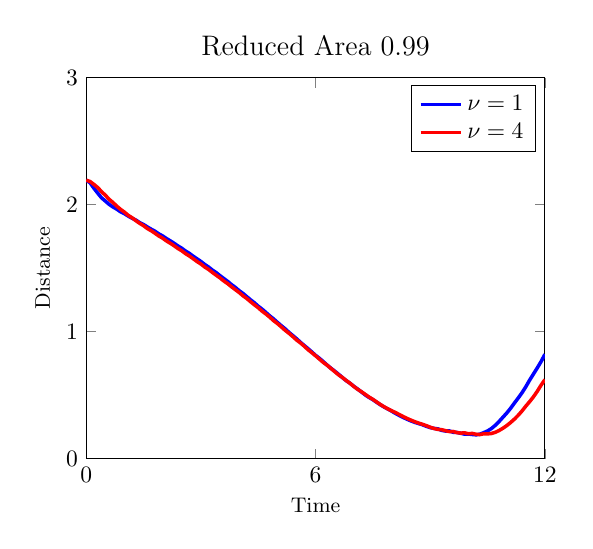
\begin{tikzpicture}[scale=0.85]

\begin{axis}[
  xmin = 0,
  xmax = 12, 
  ymin = 0,
  ymax = 3,
  xtick = {0,6,12,18,24},
  xticklabels = {$0$,$6$,$12$,$18$,$24$},
  ytick = {0,1,2,3},
  yticklabels = {$0$,$1$,$2$,$3$},
  xlabel = {Time},
  ylabel = {Distance},
  label style = {font=\small},
  legend entries = {$\nu=1$,$\nu=4$},
  title = {\large{Reduced Area 0.99}}
  ]

\addplot [mark=none,blue,line width=1.5] table{
0.0000e+00 2.1913e+00
1.0000e-01 2.1723e+00
2.0000e-01 2.1292e+00
3.0000e-01 2.0907e+00
4.0000e-01 2.0535e+00
5.0000e-01 2.0279e+00
6.0000e-01 2.0017e+00
7.0000e-01 1.9811e+00
8.0000e-01 1.9639e+00
9.0000e-01 1.9428e+00
1.0000e+00 1.9283e+00
1.1000e+00 1.9092e+00
1.2000e+00 1.8923e+00
1.3000e+00 1.8774e+00
1.4000e+00 1.8574e+00
1.5000e+00 1.8430e+00
1.6000e+00 1.8235e+00
1.7000e+00 1.8061e+00
1.8000e+00 1.7899e+00
1.9000e+00 1.7689e+00
2.0000e+00 1.7529e+00
2.1000e+00 1.7320e+00
2.2000e+00 1.7143e+00
2.3000e+00 1.6951e+00
2.4000e+00 1.6740e+00
2.5000e+00 1.6560e+00
2.6000e+00 1.6336e+00
2.7000e+00 1.6155e+00
2.8000e+00 1.5930e+00
2.9000e+00 1.5726e+00
3.0000e+00 1.5520e+00
3.1000e+00 1.5287e+00
3.2000e+00 1.5086e+00
3.3000e+00 1.4845e+00
3.4000e+00 1.4642e+00
3.5000e+00 1.4400e+00
3.6000e+00 1.4178e+00
3.7000e+00 1.3953e+00
3.8000e+00 1.3702e+00
3.9000e+00 1.3481e+00
4.0000e+00 1.3224e+00
4.1000e+00 1.3005e+00
4.2000e+00 1.2750e+00
4.3000e+00 1.2499e+00
4.4000e+00 1.2265e+00
4.5000e+00 1.1996e+00
4.6000e+00 1.1769e+00
4.7000e+00 1.1508e+00
4.8000e+00 1.1239e+00
4.9000e+00 1.1000e+00
5.0000e+00 1.0730e+00
5.1000e+00 1.0474e+00
5.2000e+00 1.0226e+00
5.3000e+00 9.9498e-01
5.4000e+00 9.6987e-01
5.5000e+00 9.4454e-01
5.6000e+00 9.1700e-01
5.7000e+00 8.9135e-01
5.8000e+00 8.6645e-01
5.9000e+00 8.4015e-01
6.0000e+00 8.1288e-01
6.1000e+00 7.8995e-01
6.2000e+00 7.6399e-01
6.3000e+00 7.3686e-01
6.4000e+00 7.1189e-01
6.5000e+00 6.8904e-01
6.6000e+00 6.6435e-01
6.7000e+00 6.3894e-01
6.8000e+00 6.1414e-01
6.9000e+00 5.9358e-01
7.0000e+00 5.6962e-01
7.1000e+00 5.4786e-01
7.2000e+00 5.2492e-01
7.3000e+00 5.0172e-01
7.4000e+00 4.8161e-01
7.5000e+00 4.6430e-01
7.6000e+00 4.4302e-01
7.7000e+00 4.2316e-01
7.8000e+00 4.0533e-01
7.9000e+00 3.8916e-01
8.0000e+00 3.7229e-01
8.1000e+00 3.5450e-01
8.2000e+00 3.3813e-01
8.3000e+00 3.2302e-01
8.4000e+00 3.0910e-01
8.5000e+00 2.9640e-01
8.6000e+00 2.8513e-01
8.7000e+00 2.7572e-01
8.8000e+00 2.6628e-01
8.9000e+00 2.5411e-01
9.0000e+00 2.4416e-01
9.1000e+00 2.3779e-01
9.2000e+00 2.3405e-01
9.3000e+00 2.2254e-01
9.4000e+00 2.1708e-01
9.5000e+00 2.1775e-01
9.6000e+00 2.0756e-01
9.7000e+00 2.0566e-01
9.8000e+00 1.9948e-01
9.9000e+00 1.9234e-01
1.0000e+01 1.9340e-01
1.0100e+01 1.8987e-01
1.0200e+01 1.8711e-01
1.0300e+01 1.9222e-01
1.0400e+01 2.0436e-01
1.0500e+01 2.1755e-01
1.0600e+01 2.3646e-01
1.0700e+01 2.6152e-01
1.0800e+01 2.9162e-01
1.0900e+01 3.2502e-01
1.1000e+01 3.5814e-01
1.1100e+01 3.9515e-01
1.1200e+01 4.3659e-01
1.1300e+01 4.7630e-01
1.1400e+01 5.1801e-01
1.1500e+01 5.6543e-01
1.1600e+01 6.1744e-01
1.1700e+01 6.6582e-01
1.1800e+01 7.1369e-01
1.1900e+01 7.6387e-01
1.2000e+01 8.2103e-01
};

\addplot [mark=none,red,line width=1.5] table{
0.0000e+00 2.1913e+00
1.0000e-01 2.1817e+00
2.0000e-01 2.1589e+00
3.0000e-01 2.1342e+00
4.0000e-01 2.1018e+00
5.0000e-01 2.0736e+00
6.0000e-01 2.0415e+00
7.0000e-01 2.0160e+00
8.0000e-01 1.9875e+00
9.0000e-01 1.9620e+00
1.0000e+00 1.9403e+00
1.1000e+00 1.9148e+00
1.2000e+00 1.8961e+00
1.3000e+00 1.8732e+00
1.4000e+00 1.8519e+00
1.5000e+00 1.8339e+00
1.6000e+00 1.8115e+00
1.7000e+00 1.7939e+00
1.8000e+00 1.7738e+00
1.9000e+00 1.7528e+00
2.0000e+00 1.7355e+00
2.1000e+00 1.7135e+00
2.2000e+00 1.6955e+00
2.3000e+00 1.6756e+00
2.4000e+00 1.6540e+00
2.5000e+00 1.6360e+00
2.6000e+00 1.6135e+00
2.7000e+00 1.5949e+00
2.8000e+00 1.5735e+00
2.9000e+00 1.5515e+00
3.0000e+00 1.5322e+00
3.1000e+00 1.5086e+00
3.2000e+00 1.4895e+00
3.3000e+00 1.4661e+00
3.4000e+00 1.4438e+00
3.5000e+00 1.4231e+00
3.6000e+00 1.3983e+00
3.7000e+00 1.3777e+00
3.8000e+00 1.3532e+00
3.9000e+00 1.3304e+00
4.0000e+00 1.3083e+00
4.1000e+00 1.2824e+00
4.2000e+00 1.2607e+00
4.3000e+00 1.2353e+00
4.4000e+00 1.2110e+00
4.5000e+00 1.1880e+00
4.6000e+00 1.1614e+00
4.7000e+00 1.1387e+00
4.8000e+00 1.1142e+00
4.9000e+00 1.0867e+00
5.0000e+00 1.0640e+00
5.1000e+00 1.0382e+00
5.2000e+00 1.0111e+00
5.3000e+00 9.8795e-01
5.4000e+00 9.6222e-01
5.5000e+00 9.3465e-01
5.6000e+00 9.1191e-01
5.7000e+00 8.8646e-01
5.8000e+00 8.5827e-01
5.9000e+00 8.3474e-01
6.0000e+00 8.0973e-01
6.1000e+00 7.8382e-01
6.2000e+00 7.5763e-01
6.3000e+00 7.3602e-01
6.4000e+00 7.1043e-01
6.5000e+00 6.8523e-01
6.6000e+00 6.5994e-01
6.7000e+00 6.3911e-01
6.8000e+00 6.1497e-01
6.9000e+00 5.9342e-01
7.0000e+00 5.6824e-01
7.1000e+00 5.4569e-01
7.2000e+00 5.2665e-01
7.3000e+00 5.0553e-01
7.4000e+00 4.8453e-01
7.5000e+00 4.6633e-01
7.6000e+00 4.4546e-01
7.7000e+00 4.2507e-01
7.8000e+00 4.0679e-01
7.9000e+00 3.9031e-01
8.0000e+00 3.7528e-01
8.1000e+00 3.6137e-01
8.2000e+00 3.4531e-01
8.3000e+00 3.2981e-01
8.4000e+00 3.1546e-01
8.5000e+00 3.0219e-01
8.6000e+00 2.9003e-01
8.7000e+00 2.7918e-01
8.8000e+00 2.6998e-01
8.9000e+00 2.5898e-01
9.0000e+00 2.4707e-01
9.1000e+00 2.3697e-01
9.2000e+00 2.2993e-01
9.3000e+00 2.2740e-01
9.4000e+00 2.1976e-01
9.5000e+00 2.1290e-01
9.6000e+00 2.1336e-01
9.7000e+00 2.0430e-01
9.8000e+00 2.0095e-01
9.9000e+00 2.0285e-01
1.0000e+01 1.9587e-01
1.0100e+01 1.9848e-01
1.0200e+01 1.9158e-01
1.0300e+01 1.8957e-01
1.0400e+01 1.9553e-01
1.0500e+01 1.9473e-01
1.0600e+01 1.9764e-01
1.0700e+01 2.0683e-01
1.0800e+01 2.2094e-01
1.0900e+01 2.3880e-01
1.1000e+01 2.5941e-01
1.1100e+01 2.8354e-01
1.1200e+01 3.1037e-01
1.1300e+01 3.4058e-01
1.1400e+01 3.7458e-01
1.1500e+01 4.1277e-01
1.1600e+01 4.4817e-01
1.1700e+01 4.8637e-01
1.1800e+01 5.2970e-01
1.1900e+01 5.7822e-01
1.2000e+01 6.2177e-01
};

\end{axis}

%\draw[gray,thin] (0,0) grid +(3,4);

\end{tikzpicture}


\fi
\end{tabular}
\mcaption{Two vesicles are submerged in a shear flow.  In the first and
second rows, the vesicles have reduced area 0.65, and in the third and
fourth rows, the vesicles have reduced area 0.99.  Each simulation is
done with viscosity contrasts $\nu=1$ and $\nu=4$.  The bottom plots
show the distance between the vesicles for both reduced areas and both
viscosity contrasts.  Comparing semi-implicit inter-vesicle interactions
with both first- and second-order time stepping, the distance between
the vesicles never differ by more than 2.2\% for both reduced areas and
both viscosity contrasts.}{f:shear:reducedAreas} 
\end{figure}

We now do a convergence study for both values of the reduced area and
viscosity contrast.  We vary the number of points per vesicle, the
number of time steps, and the time integrator.  We report the errors in
area and length at the time horizon $t=12$ in Tables~\ref{t:shear:RA65}
and~\ref{t:shear:RA99}.  First, we see that first- and second-order
convergence is achieved for all combinations of reduced area and
viscosity contrast.  Second, semi-implicit inter-vesicle interactions
do not improve the accuracy of first-order time stepping, but, we will
see later that this time integrator is more stable.

\begin{table}[htp]
\centering
\begin{tabular}{ccc|cc|cc} 
Time & & & \multicolumn{2}{c|}{$\nu=1$} & \multicolumn{2}{c}{$\nu=4$} \\
Integrator   & $N$ & $\Delta t$ & $e_{A}$   & $e_{L}$   & 
$e_{A}$   & $e_{L}$ \\ 
\hline

Explicit (1) & 32  & 0.04       & $6.73e-2$ & $5.21e-2$ &
$4.07e-2$ & $2.41e-2$ \\ 

Explicit (1) & 64  & 0.02       & $3.36e-2$ & $2.62e-2$ &
$2.02e-2$ & $1.20e-2$ \\ 

Explicit (1) & 128 & 0.01       & $1.68e-2$ & $1.31e-2$ &
$1.01e-2$ & $5.99e-2$ \\ 
\hline

Implicit (1) & 32  & 0.04       & $6.73e-2$ & $5.21e-2$ &
$4.06e-2$ & $2.40e-2$ \\ 

Implicit (1) & 64  & 0.02       & $3.36e-2$ & $2.62e-2$ &
$2.02e-2$ & $1.20e-2$ \\ 

Implicit (1) & 128 & 0.01       & $1.68e-2$ & $1.31e-2$ &
$1.02-2$ & $5.98e-3$ \\ 
\hline

Implicit (2) & 32  & 0.04       & $1.59e-4$ & $3.21e-4$ &
$2.69e-5$ & $6.33e-5$ \\ 

Implicit (2) & 64  & 0.02       & $3.87e-6$ & $6.52e-5$ &
$3.78e-6$ & $1.20e-5$ \\ 

Implicit (2) & 128 & 0.01       & $2.79e-7$ & $1.47e-5$ &
$3.85e-7$ & $2.28e-6$ 
\end{tabular}
\mcaption{The errors in area and length at $t=12$ for different time
integrators applied to two vesicles of reduced area $0.65$ in a shear
flow.  The parenthetic values are the time stepping order.  Results are
presented for no viscosity contrast and a viscosity contrast of
4.}{t:shear:RA65}

\begin{tabular}{ccc|cc|cc} 
Time & & & \multicolumn{2}{c|}{$\nu=1$} & \multicolumn{2}{c}{$\nu=4$} \\
Integrator   & $N$ & $\Delta t$ & $e_{A}$   & $e_{L}$   & 
$e_{A}$   & $e_{L}$ \\ 
\hline

Explicit (1) & 32  & 0.04       & $1.05e-1$ & $5.48e-2$ &
$9.67e-2$ & $4.94e-2$ \\ 

Explicit (1) & 64  & 0.02       & $5.15e-2$ & $2.70e-2$ &
$4.78e-2$ & $2.45e-2$ \\ 

Explicit (1) & 128 & 0.01       & $2.55e-2$ & $1.34e-2$ &
$2.37e-2$ & $1.22e-2$ \\ 
\hline

Implicit (1) & 32  & 0.04       & $1.05e-1$ & $5.48e-2$ &
$9.69e-2$ & $4.93e-2$ \\ 

Implicit (1) & 64  & 0.02       & $5.16e-2$ & $2.70e-2$ &
$4.77e-2$ & $2.45e-2$ \\ 

Implicit (1) & 128 & 0.01       & $2.55e-2$ & $1.34e-2$ &
$2.36e-2$ & $1.22e-2$ \\ 
\hline

Implicit (2) & 32  & 0.04       & $2.40e-5$ & $1.13e-4$ &
$5.85e-5$ & $4.68e-5$ \\ 

Implicit (2) & 64  & 0.02       & $1.65e-6$ & $1.50e-5$ &
$7.05e-6$ & $5.86e-6$ \\ 

Implicit (2) & 128 & 0.01       & $1.56e-7$ & $1.92e-6$ &
$8.62e-7$ & $7.26e-7$ 

\end{tabular}

\mcaption{The errors in area and length at $t=12$ for different time
integrators applied to two vesicles of reduced area $0.99$ in a shear
flow.  The parenthetic values are the time stepping order.  Results are
presented for no viscosity contrast and a viscosity contrast of
4.}{t:shear:RA99}
\end{table}

%%%%%%%%%%%%%%%%%%%%%%%%%%%%%%%%%%%%%%%%%%%%%%%%%%%%%%%%%%%%%%%%%%%%%%%%%%%
\subsection{Taylor-Green Flow}
\label{s:taylorGreen}
We consider the Taylor-Green flow $\uu = (\sin x \cos y,-\cos x \sin
y)$ with 9 vesicles each with $N=64$ points of reduced area 0.65 placed
inside the periodic cell $(0,2\pi)^{2}$ (left plot of
Figure~\ref{f:taylorGreen:collision}).  We consider first-order IMEX
Euler with both semi-implicit and explicit inter-vesicle interactions.
We find the largest time step of both methods so that the vesicles do
not cross before a time horizon of $T = 1$.  With explicit
interactions, the vesicles cross if $74$ time steps are taken but not
if $75$ time steps are taken.  However, with semi-implicit
interactions, the simulation successfully completes even with one time
step.  Of course the error is too large and a time step size this large
is unreasonable.

\begin{figure}[htp]
\begin{center}
  \begin{tabular}{ccc}
    \ifInputs
    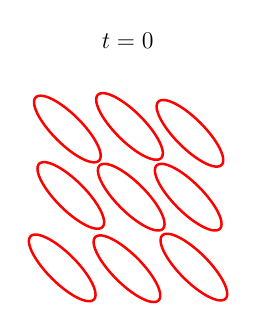
\begin{tikzpicture}[scale=0.6]

\begin{axis}[
  xmin = 0,
  xmax = 3.14,
  ymin = 0,
  ymax = 3.14,
  axis equal = true,
  hide axis,
  title = {\Large$t=0$}
  ]

\addplot [mark=none,red,line width=1.5] table{
1.1748e+00 3.9602e-01
1.1849e+00 4.0974e-01
1.1914e+00 4.2689e-01
1.1942e+00 4.4729e-01
1.1933e+00 4.7076e-01
1.1886e+00 4.9707e-01
1.1802e+00 5.2596e-01
1.1682e+00 5.5716e-01
1.1527e+00 5.9036e-01
1.1339e+00 6.2524e-01
1.1119e+00 6.6148e-01
1.0870e+00 6.9872e-01
1.0593e+00 7.3660e-01
1.0292e+00 7.7476e-01
9.9695e-01 8.1282e-01
9.6284e-01 8.5043e-01
9.2723e-01 8.8723e-01
8.9043e-01 9.2284e-01
8.5282e-01 9.5695e-01
8.1476e-01 9.8920e-01
7.7660e-01 1.0193e+00
7.3872e-01 1.0470e+00
7.0148e-01 1.0719e+00
6.6524e-01 1.0939e+00
6.3036e-01 1.1127e+00
5.9716e-01 1.1282e+00
5.6596e-01 1.1402e+00
5.3707e-01 1.1486e+00
5.1076e-01 1.1533e+00
4.8729e-01 1.1542e+00
4.6689e-01 1.1514e+00
4.4974e-01 1.1449e+00
4.3602e-01 1.1348e+00
4.2586e-01 1.1211e+00
4.1935e-01 1.1039e+00
4.1656e-01 1.0835e+00
4.1752e-01 1.0600e+00
4.2221e-01 1.0337e+00
4.3059e-01 1.0048e+00
4.4258e-01 9.7364e-01
4.5807e-01 9.4044e-01
4.7690e-01 9.0555e-01
4.9889e-01 8.6932e-01
5.2383e-01 8.3208e-01
5.5149e-01 7.9420e-01
5.8159e-01 7.5604e-01
6.1385e-01 7.1797e-01
6.4795e-01 6.8036e-01
6.8357e-01 6.4357e-01
7.2036e-01 6.0795e-01
7.5797e-01 5.7385e-01
7.9604e-01 5.4159e-01
8.3420e-01 5.1149e-01
8.7208e-01 4.8383e-01
9.0932e-01 4.5889e-01
9.4555e-01 4.3690e-01
9.8044e-01 4.1807e-01
1.0136e+00 4.0258e-01
1.0448e+00 3.9059e-01
1.0737e+00 3.8221e-01
1.1000e+00 3.7752e-01
1.1235e+00 3.7656e-01
1.1439e+00 3.7935e-01
1.1611e+00 3.8586e-01
1.1748e+00 3.9602e-01
};

\addplot [mark=none,red,line width=1.5] table{
1.9302e+00 3.8602e-01
1.9403e+00 3.9974e-01
1.9468e+00 4.1689e-01
1.9496e+00 4.3729e-01
1.9487e+00 4.6076e-01
1.9440e+00 4.8707e-01
1.9356e+00 5.1596e-01
1.9236e+00 5.4716e-01
1.9081e+00 5.8036e-01
1.8893e+00 6.1524e-01
1.8673e+00 6.5148e-01
1.8424e+00 6.8872e-01
1.8147e+00 7.2660e-01
1.7846e+00 7.6476e-01
1.7523e+00 8.0282e-01
1.7182e+00 8.4043e-01
1.6826e+00 8.7723e-01
1.6458e+00 9.1284e-01
1.6082e+00 9.4695e-01
1.5702e+00 9.7920e-01
1.5320e+00 1.0093e+00
1.4941e+00 1.0370e+00
1.4569e+00 1.0619e+00
1.4206e+00 1.0839e+00
1.3858e+00 1.1027e+00
1.3526e+00 1.1182e+00
1.3214e+00 1.1302e+00
1.2925e+00 1.1386e+00
1.2662e+00 1.1433e+00
1.2427e+00 1.1442e+00
1.2223e+00 1.1414e+00
1.2051e+00 1.1349e+00
1.1914e+00 1.1248e+00
1.1813e+00 1.1111e+00
1.1748e+00 1.0939e+00
1.1720e+00 1.0735e+00
1.1729e+00 1.0500e+00
1.1776e+00 1.0237e+00
1.1860e+00 9.9484e-01
1.1980e+00 9.6364e-01
1.2135e+00 9.3044e-01
1.2323e+00 8.9555e-01
1.2543e+00 8.5932e-01
1.2792e+00 8.2208e-01
1.3069e+00 7.8420e-01
1.3370e+00 7.4604e-01
1.3692e+00 7.0797e-01
1.4034e+00 6.7036e-01
1.4390e+00 6.3357e-01
1.4758e+00 5.9795e-01
1.5134e+00 5.6385e-01
1.5514e+00 5.3159e-01
1.5896e+00 5.0149e-01
1.6275e+00 4.7383e-01
1.6647e+00 4.4889e-01
1.7010e+00 4.2690e-01
1.7358e+00 4.0807e-01
1.7690e+00 3.9258e-01
1.8002e+00 3.8059e-01
1.8291e+00 3.7221e-01
1.8554e+00 3.6752e-01
1.8789e+00 3.6656e-01
1.8993e+00 3.6935e-01
1.9165e+00 3.7586e-01
1.9302e+00 3.8602e-01
};

\addplot [mark=none,red,line width=1.5] table{
2.7116e+00 4.0502e-01
2.7217e+00 4.1874e-01
2.7282e+00 4.3589e-01
2.7310e+00 4.5629e-01
2.7301e+00 4.7976e-01
2.7254e+00 5.0607e-01
2.7170e+00 5.3496e-01
2.7050e+00 5.6616e-01
2.6895e+00 5.9936e-01
2.6707e+00 6.3424e-01
2.6487e+00 6.7048e-01
2.6238e+00 7.0772e-01
2.5961e+00 7.4560e-01
2.5660e+00 7.8376e-01
2.5337e+00 8.2182e-01
2.4996e+00 8.5943e-01
2.4640e+00 8.9623e-01
2.4272e+00 9.3184e-01
2.3896e+00 9.6595e-01
2.3516e+00 9.9820e-01
2.3134e+00 1.0283e+00
2.2755e+00 1.0560e+00
2.2383e+00 1.0809e+00
2.2020e+00 1.1029e+00
2.1672e+00 1.1217e+00
2.1340e+00 1.1372e+00
2.1028e+00 1.1492e+00
2.0739e+00 1.1576e+00
2.0476e+00 1.1623e+00
2.0241e+00 1.1632e+00
2.0037e+00 1.1604e+00
1.9865e+00 1.1539e+00
1.9728e+00 1.1438e+00
1.9627e+00 1.1301e+00
1.9562e+00 1.1129e+00
1.9534e+00 1.0925e+00
1.9543e+00 1.0690e+00
1.9590e+00 1.0427e+00
1.9674e+00 1.0138e+00
1.9794e+00 9.8264e-01
1.9949e+00 9.4944e-01
2.0137e+00 9.1455e-01
2.0357e+00 8.7832e-01
2.0606e+00 8.4108e-01
2.0883e+00 8.0320e-01
2.1184e+00 7.6504e-01
2.1506e+00 7.2697e-01
2.1847e+00 6.8936e-01
2.2204e+00 6.5257e-01
2.2572e+00 6.1695e-01
2.2948e+00 5.8285e-01
2.3328e+00 5.5059e-01
2.3710e+00 5.2049e-01
2.4089e+00 4.9283e-01
2.4461e+00 4.6789e-01
2.4823e+00 4.4590e-01
2.5172e+00 4.2707e-01
2.5504e+00 4.1158e-01
2.5816e+00 3.9959e-01
2.6105e+00 3.9121e-01
2.6368e+00 3.8652e-01
2.6603e+00 3.8556e-01
2.6807e+00 3.8835e-01
2.6978e+00 3.9486e-01
2.7116e+00 4.0502e-01
};

\addplot [mark=none,red,line width=1.5] table{
1.2748e+00 1.2414e+00
1.2849e+00 1.2551e+00
1.2914e+00 1.2723e+00
1.2942e+00 1.2927e+00
1.2933e+00 1.3162e+00
1.2886e+00 1.3425e+00
1.2802e+00 1.3714e+00
1.2682e+00 1.4026e+00
1.2527e+00 1.4358e+00
1.2339e+00 1.4706e+00
1.2119e+00 1.5069e+00
1.1870e+00 1.5441e+00
1.1593e+00 1.5820e+00
1.1292e+00 1.6202e+00
1.0969e+00 1.6582e+00
1.0628e+00 1.6958e+00
1.0272e+00 1.7326e+00
9.9043e-01 1.7682e+00
9.5282e-01 1.8023e+00
9.1476e-01 1.8346e+00
8.7660e-01 1.8647e+00
8.3872e-01 1.8924e+00
8.0148e-01 1.9173e+00
7.6524e-01 1.9393e+00
7.3036e-01 1.9581e+00
6.9716e-01 1.9736e+00
6.6596e-01 1.9856e+00
6.3707e-01 1.9940e+00
6.1076e-01 1.9987e+00
5.8729e-01 1.9996e+00
5.6689e-01 1.9968e+00
5.4974e-01 1.9903e+00
5.3602e-01 1.9802e+00
5.2586e-01 1.9665e+00
5.1935e-01 1.9493e+00
5.1656e-01 1.9289e+00
5.1752e-01 1.9054e+00
5.2221e-01 1.8791e+00
5.3059e-01 1.8502e+00
5.4258e-01 1.8190e+00
5.5807e-01 1.7858e+00
5.7690e-01 1.7510e+00
5.9889e-01 1.7147e+00
6.2383e-01 1.6775e+00
6.5149e-01 1.6396e+00
6.8159e-01 1.6014e+00
7.1385e-01 1.5634e+00
7.4795e-01 1.5258e+00
7.8357e-01 1.4890e+00
8.2036e-01 1.4534e+00
8.5797e-01 1.4192e+00
8.9604e-01 1.3870e+00
9.3420e-01 1.3569e+00
9.7208e-01 1.3292e+00
1.0093e+00 1.3043e+00
1.0456e+00 1.2823e+00
1.0804e+00 1.2635e+00
1.1136e+00 1.2480e+00
1.1448e+00 1.2360e+00
1.1737e+00 1.2276e+00
1.2000e+00 1.2229e+00
1.2235e+00 1.2220e+00
1.2439e+00 1.2248e+00
1.2611e+00 1.2313e+00
1.2748e+00 1.2414e+00
};

\addplot [mark=none,red,line width=1.5] table{
1.9802e+00 1.2214e+00
1.9903e+00 1.2351e+00
1.9968e+00 1.2523e+00
1.9996e+00 1.2727e+00
1.9987e+00 1.2962e+00
1.9940e+00 1.3225e+00
1.9856e+00 1.3514e+00
1.9736e+00 1.3826e+00
1.9581e+00 1.4158e+00
1.9393e+00 1.4506e+00
1.9173e+00 1.4869e+00
1.8924e+00 1.5241e+00
1.8647e+00 1.5620e+00
1.8346e+00 1.6002e+00
1.8023e+00 1.6382e+00
1.7682e+00 1.6758e+00
1.7326e+00 1.7126e+00
1.6958e+00 1.7482e+00
1.6582e+00 1.7823e+00
1.6202e+00 1.8146e+00
1.5820e+00 1.8447e+00
1.5441e+00 1.8724e+00
1.5069e+00 1.8973e+00
1.4706e+00 1.9193e+00
1.4358e+00 1.9381e+00
1.4026e+00 1.9536e+00
1.3714e+00 1.9656e+00
1.3425e+00 1.9740e+00
1.3162e+00 1.9787e+00
1.2927e+00 1.9796e+00
1.2723e+00 1.9768e+00
1.2551e+00 1.9703e+00
1.2414e+00 1.9602e+00
1.2313e+00 1.9465e+00
1.2248e+00 1.9293e+00
1.2220e+00 1.9089e+00
1.2229e+00 1.8854e+00
1.2276e+00 1.8591e+00
1.2360e+00 1.8302e+00
1.2480e+00 1.7990e+00
1.2635e+00 1.7658e+00
1.2823e+00 1.7310e+00
1.3043e+00 1.6947e+00
1.3292e+00 1.6575e+00
1.3569e+00 1.6196e+00
1.3870e+00 1.5814e+00
1.4192e+00 1.5434e+00
1.4534e+00 1.5058e+00
1.4890e+00 1.4690e+00
1.5258e+00 1.4334e+00
1.5634e+00 1.3992e+00
1.6014e+00 1.3670e+00
1.6396e+00 1.3369e+00
1.6775e+00 1.3092e+00
1.7147e+00 1.2843e+00
1.7510e+00 1.2623e+00
1.7858e+00 1.2435e+00
1.8190e+00 1.2280e+00
1.8502e+00 1.2160e+00
1.8791e+00 1.2076e+00
1.9054e+00 1.2029e+00
1.9289e+00 1.2020e+00
1.9493e+00 1.2048e+00
1.9665e+00 1.2113e+00
1.9802e+00 1.2214e+00
};

\addplot [mark=none,red,line width=1.5] table{
2.6456e+00 1.2214e+00
2.6557e+00 1.2351e+00
2.6622e+00 1.2523e+00
2.6650e+00 1.2727e+00
2.6641e+00 1.2962e+00
2.6594e+00 1.3225e+00
2.6510e+00 1.3514e+00
2.6390e+00 1.3826e+00
2.6235e+00 1.4158e+00
2.6047e+00 1.4506e+00
2.5827e+00 1.4869e+00
2.5578e+00 1.5241e+00
2.5301e+00 1.5620e+00
2.5000e+00 1.6002e+00
2.4677e+00 1.6382e+00
2.4336e+00 1.6758e+00
2.3980e+00 1.7126e+00
2.3612e+00 1.7482e+00
2.3236e+00 1.7823e+00
2.2856e+00 1.8146e+00
2.2474e+00 1.8447e+00
2.2095e+00 1.8724e+00
2.1723e+00 1.8973e+00
2.1360e+00 1.9193e+00
2.1012e+00 1.9381e+00
2.0680e+00 1.9536e+00
2.0368e+00 1.9656e+00
2.0079e+00 1.9740e+00
1.9816e+00 1.9787e+00
1.9581e+00 1.9796e+00
1.9377e+00 1.9768e+00
1.9205e+00 1.9703e+00
1.9068e+00 1.9602e+00
1.8967e+00 1.9465e+00
1.8902e+00 1.9293e+00
1.8874e+00 1.9089e+00
1.8883e+00 1.8854e+00
1.8930e+00 1.8591e+00
1.9014e+00 1.8302e+00
1.9134e+00 1.7990e+00
1.9289e+00 1.7658e+00
1.9477e+00 1.7310e+00
1.9697e+00 1.6947e+00
1.9946e+00 1.6575e+00
2.0223e+00 1.6196e+00
2.0524e+00 1.5814e+00
2.0846e+00 1.5434e+00
2.1187e+00 1.5058e+00
2.1544e+00 1.4690e+00
2.1912e+00 1.4334e+00
2.2288e+00 1.3992e+00
2.2668e+00 1.3670e+00
2.3050e+00 1.3369e+00
2.3429e+00 1.3092e+00
2.3801e+00 1.2843e+00
2.4163e+00 1.2623e+00
2.4512e+00 1.2435e+00
2.4844e+00 1.2280e+00
2.5156e+00 1.2160e+00
2.5445e+00 1.2076e+00
2.5708e+00 1.2029e+00
2.5943e+00 1.2020e+00
2.6147e+00 1.2048e+00
2.6318e+00 1.2113e+00
2.6456e+00 1.2214e+00
};

\addplot [mark=none,red,line width=1.5] table{
1.2348e+00 2.0168e+00
1.2449e+00 2.0305e+00
1.2514e+00 2.0477e+00
1.2542e+00 2.0681e+00
1.2533e+00 2.0916e+00
1.2486e+00 2.1179e+00
1.2402e+00 2.1468e+00
1.2282e+00 2.1780e+00
1.2127e+00 2.2112e+00
1.1939e+00 2.2460e+00
1.1719e+00 2.2823e+00
1.1470e+00 2.3195e+00
1.1193e+00 2.3574e+00
1.0892e+00 2.3956e+00
1.0569e+00 2.4336e+00
1.0228e+00 2.4712e+00
9.8723e-01 2.5080e+00
9.5043e-01 2.5436e+00
9.1282e-01 2.5777e+00
8.7476e-01 2.6100e+00
8.3660e-01 2.6401e+00
7.9872e-01 2.6678e+00
7.6148e-01 2.6927e+00
7.2524e-01 2.7147e+00
6.9036e-01 2.7335e+00
6.5716e-01 2.7490e+00
6.2596e-01 2.7610e+00
5.9707e-01 2.7694e+00
5.7076e-01 2.7741e+00
5.4729e-01 2.7750e+00
5.2689e-01 2.7722e+00
5.0974e-01 2.7657e+00
4.9602e-01 2.7556e+00
4.8586e-01 2.7418e+00
4.7935e-01 2.7247e+00
4.7656e-01 2.7043e+00
4.7752e-01 2.6808e+00
4.8221e-01 2.6545e+00
4.9059e-01 2.6256e+00
5.0258e-01 2.5944e+00
5.1807e-01 2.5612e+00
5.3690e-01 2.5263e+00
5.5889e-01 2.4901e+00
5.8383e-01 2.4529e+00
6.1149e-01 2.4150e+00
6.4159e-01 2.3768e+00
6.7385e-01 2.3388e+00
7.0795e-01 2.3012e+00
7.4357e-01 2.2644e+00
7.8036e-01 2.2287e+00
8.1797e-01 2.1946e+00
8.5604e-01 2.1624e+00
8.9420e-01 2.1323e+00
9.3208e-01 2.1046e+00
9.6932e-01 2.0797e+00
1.0056e+00 2.0577e+00
1.0404e+00 2.0389e+00
1.0736e+00 2.0234e+00
1.1048e+00 2.0114e+00
1.1337e+00 2.0030e+00
1.1600e+00 1.9983e+00
1.1835e+00 1.9974e+00
1.2039e+00 2.0002e+00
1.2211e+00 2.0067e+00
1.2348e+00 2.0168e+00
};

\addplot [mark=none,red,line width=1.5] table{
1.9602e+00 2.0468e+00
1.9703e+00 2.0605e+00
1.9768e+00 2.0777e+00
1.9796e+00 2.0981e+00
1.9787e+00 2.1216e+00
1.9740e+00 2.1479e+00
1.9656e+00 2.1768e+00
1.9536e+00 2.2080e+00
1.9381e+00 2.2412e+00
1.9193e+00 2.2760e+00
1.8973e+00 2.3123e+00
1.8724e+00 2.3495e+00
1.8447e+00 2.3874e+00
1.8146e+00 2.4256e+00
1.7823e+00 2.4636e+00
1.7482e+00 2.5012e+00
1.7126e+00 2.5380e+00
1.6758e+00 2.5736e+00
1.6382e+00 2.6077e+00
1.6002e+00 2.6400e+00
1.5620e+00 2.6701e+00
1.5241e+00 2.6978e+00
1.4869e+00 2.7227e+00
1.4506e+00 2.7447e+00
1.4158e+00 2.7635e+00
1.3826e+00 2.7790e+00
1.3514e+00 2.7910e+00
1.3225e+00 2.7994e+00
1.2962e+00 2.8041e+00
1.2727e+00 2.8050e+00
1.2523e+00 2.8022e+00
1.2351e+00 2.7957e+00
1.2214e+00 2.7856e+00
1.2113e+00 2.7718e+00
1.2048e+00 2.7547e+00
1.2020e+00 2.7343e+00
1.2029e+00 2.7108e+00
1.2076e+00 2.6845e+00
1.2160e+00 2.6556e+00
1.2280e+00 2.6244e+00
1.2435e+00 2.5912e+00
1.2623e+00 2.5563e+00
1.2843e+00 2.5201e+00
1.3092e+00 2.4829e+00
1.3369e+00 2.4450e+00
1.3670e+00 2.4068e+00
1.3992e+00 2.3688e+00
1.4334e+00 2.3312e+00
1.4690e+00 2.2944e+00
1.5058e+00 2.2587e+00
1.5434e+00 2.2246e+00
1.5814e+00 2.1924e+00
1.6196e+00 2.1623e+00
1.6575e+00 2.1346e+00
1.6947e+00 2.1097e+00
1.7310e+00 2.0877e+00
1.7658e+00 2.0689e+00
1.7990e+00 2.0534e+00
1.8302e+00 2.0414e+00
1.8591e+00 2.0330e+00
1.8854e+00 2.0283e+00
1.9089e+00 2.0274e+00
1.9293e+00 2.0302e+00
1.9465e+00 2.0367e+00
1.9602e+00 2.0468e+00
};

\addplot [mark=none,red,line width=1.5] table{
2.6656e+00 1.9668e+00
2.6757e+00 1.9805e+00
2.6822e+00 1.9977e+00
2.6850e+00 2.0181e+00
2.6841e+00 2.0416e+00
2.6794e+00 2.0679e+00
2.6710e+00 2.0968e+00
2.6590e+00 2.1280e+00
2.6435e+00 2.1612e+00
2.6247e+00 2.1960e+00
2.6027e+00 2.2323e+00
2.5778e+00 2.2695e+00
2.5501e+00 2.3074e+00
2.5200e+00 2.3456e+00
2.4877e+00 2.3836e+00
2.4536e+00 2.4212e+00
2.4180e+00 2.4580e+00
2.3812e+00 2.4936e+00
2.3436e+00 2.5277e+00
2.3056e+00 2.5600e+00
2.2674e+00 2.5901e+00
2.2295e+00 2.6178e+00
2.1923e+00 2.6427e+00
2.1560e+00 2.6647e+00
2.1212e+00 2.6835e+00
2.0880e+00 2.6990e+00
2.0568e+00 2.7110e+00
2.0279e+00 2.7194e+00
2.0016e+00 2.7241e+00
1.9781e+00 2.7250e+00
1.9577e+00 2.7222e+00
1.9405e+00 2.7157e+00
1.9268e+00 2.7056e+00
1.9167e+00 2.6918e+00
1.9102e+00 2.6747e+00
1.9074e+00 2.6543e+00
1.9083e+00 2.6308e+00
1.9130e+00 2.6045e+00
1.9214e+00 2.5756e+00
1.9334e+00 2.5444e+00
1.9489e+00 2.5112e+00
1.9677e+00 2.4763e+00
1.9897e+00 2.4401e+00
2.0146e+00 2.4029e+00
2.0423e+00 2.3650e+00
2.0724e+00 2.3268e+00
2.1046e+00 2.2888e+00
2.1387e+00 2.2512e+00
2.1744e+00 2.2144e+00
2.2112e+00 2.1787e+00
2.2488e+00 2.1446e+00
2.2868e+00 2.1124e+00
2.3250e+00 2.0823e+00
2.3629e+00 2.0546e+00
2.4001e+00 2.0297e+00
2.4363e+00 2.0077e+00
2.4712e+00 1.9889e+00
2.5044e+00 1.9734e+00
2.5356e+00 1.9614e+00
2.5645e+00 1.9530e+00
2.5908e+00 1.9483e+00
2.6143e+00 1.9474e+00
2.6347e+00 1.9502e+00
2.6518e+00 1.9567e+00
2.6656e+00 1.9668e+00
};


\end{axis}

%\draw[gray,thin] (0,0) grid +(3,4);

\end{tikzpicture}

 &
    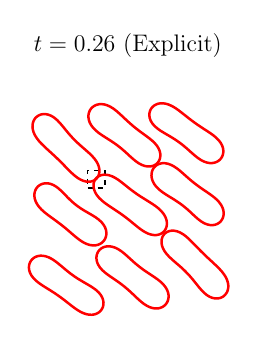
\begin{tikzpicture}[scale=0.6]

\begin{axis}[
  xmin = 0,
  xmax = 3.14,
  ymin = 0,
  ymax = 3.14,
  axis equal = true,
  hide axis,
  title = {\Large$t=0.26$ (Explicit)}
  ]

\addplot [mark=none,black,line width=1.0,dashed] table{
  1.1 1.8
  1.3 1.8
  1.3 2.0
  1.1 2.0
  1.1 1.8
};

\addplot [mark=none,red,line width=1.5] table{
1.2484e+00 3.5939e-01
1.2596e+00 3.7238e-01
1.2697e+00 3.8794e-01
1.2783e+00 4.0701e-01
1.2843e+00 4.3005e-01
1.2861e+00 4.5688e-01
1.2822e+00 4.8673e-01
1.2714e+00 5.1832e-01
1.2530e+00 5.5006e-01
1.2274e+00 5.8058e-01
1.1956e+00 6.0907e-01
1.1588e+00 6.3552e-01
1.1185e+00 6.6058e-01
1.0761e+00 6.8522e-01
1.0326e+00 7.1045e-01
9.8899e-01 7.3701e-01
9.4611e-01 7.6529e-01
9.0450e-01 7.9526e-01
8.6447e-01 8.2651e-01
8.2602e-01 8.5834e-01
7.8889e-01 8.8977e-01
7.5266e-01 9.1964e-01
7.1684e-01 9.4672e-01
6.8116e-01 9.6976e-01
6.4573e-01 9.8769e-01
6.1110e-01 9.9979e-01
5.7817e-01 1.0059e+00
5.4796e-01 1.0065e+00
5.2128e-01 1.0025e+00
4.9860e-01 9.9509e-01
4.7992e-01 9.8562e-01
4.6472e-01 9.7497e-01
4.5210e-01 9.6334e-01
4.4111e-01 9.5018e-01
4.3126e-01 9.3449e-01
4.2291e-01 9.1535e-01
4.1715e-01 8.9230e-01
4.1545e-01 8.6548e-01
4.1928e-01 8.3561e-01
4.2980e-01 8.0390e-01
4.4752e-01 7.7180e-01
4.7217e-01 7.4060e-01
5.0288e-01 7.1106e-01
5.3844e-01 6.8324e-01
5.7754e-01 6.5667e-01
6.1896e-01 6.3055e-01
6.6163e-01 6.0409e-01
7.0465e-01 5.7670e-01
7.4730e-01 5.4809e-01
7.8906e-01 5.1832e-01
8.2964e-01 4.8776e-01
8.6897e-01 4.5703e-01
9.0719e-01 4.2700e-01
9.4459e-01 3.9867e-01
9.8146e-01 3.7313e-01
1.0180e+00 3.5147e-01
1.0539e+00 3.3466e-01
1.0888e+00 3.2334e-01
1.1218e+00 3.1765e-01
1.1521e+00 3.1722e-01
1.1787e+00 3.2117e-01
1.2015e+00 3.2834e-01
1.2202e+00 3.3756e-01
1.2356e+00 3.4798e-01
1.2484e+00 3.5939e-01
};

\addplot [mark=none,red,line width=1.5] table{
2.0184e+00 4.4666e-01
2.0278e+00 4.6103e-01
2.0358e+00 4.7771e-01
2.0420e+00 4.9757e-01
2.0456e+00 5.2100e-01
2.0452e+00 5.4782e-01
2.0396e+00 5.7740e-01
2.0278e+00 6.0866e-01
2.0094e+00 6.4038e-01
1.9845e+00 6.7144e-01
1.9539e+00 7.0114e-01
1.9186e+00 7.2938e-01
1.8800e+00 7.5660e-01
1.8391e+00 7.8360e-01
1.7972e+00 8.1120e-01
1.7552e+00 8.4008e-01
1.7140e+00 8.7058e-01
1.6740e+00 9.0263e-01
1.6355e+00 9.3579e-01
1.5985e+00 9.6929e-01
1.5626e+00 1.0021e+00
1.5272e+00 1.0330e+00
1.4918e+00 1.0607e+00
1.4560e+00 1.0838e+00
1.4202e+00 1.1012e+00
1.3851e+00 1.1121e+00
1.3519e+00 1.1166e+00
1.3216e+00 1.1151e+00
1.2951e+00 1.1089e+00
1.2730e+00 1.0994e+00
1.2552e+00 1.0879e+00
1.2412e+00 1.0755e+00
1.2299e+00 1.0624e+00
1.2206e+00 1.0481e+00
1.2127e+00 1.0314e+00
1.2066e+00 1.0115e+00
1.2035e+00 9.8796e-01
1.2046e+00 9.6114e-01
1.2112e+00 9.3179e-01
1.2242e+00 9.0104e-01
1.2440e+00 8.7015e-01
1.2701e+00 8.4010e-01
1.3017e+00 8.1137e-01
1.3375e+00 7.8377e-01
1.3762e+00 7.5666e-01
1.4167e+00 7.2920e-01
1.4579e+00 7.0064e-01
1.4989e+00 6.7049e-01
1.5391e+00 6.3863e-01
1.5780e+00 6.0527e-01
1.6154e+00 5.7100e-01
1.6516e+00 5.3663e-01
1.6870e+00 5.0324e-01
1.7221e+00 4.7204e-01
1.7574e+00 4.4436e-01
1.7931e+00 4.2150e-01
1.8290e+00 4.0456e-01
1.8642e+00 3.9419e-01
1.8976e+00 3.9043e-01
1.9278e+00 3.9256e-01
1.9541e+00 3.9937e-01
1.9759e+00 4.0933e-01
1.9934e+00 4.2105e-01
2.0073e+00 4.3355e-01
2.0184e+00 4.4666e-01
};

\addplot [mark=none,red,line width=1.5] table{
2.7136e+00 5.5896e-01
2.7231e+00 5.7318e-01
2.7314e+00 5.8973e-01
2.7380e+00 6.0946e-01
2.7422e+00 6.3281e-01
2.7429e+00 6.5966e-01
2.7388e+00 6.8953e-01
2.7293e+00 7.2159e-01
2.7140e+00 7.5490e-01
2.6931e+00 7.8861e-01
2.6671e+00 8.2221e-01
2.6370e+00 8.5552e-01
2.6037e+00 8.8871e-01
2.5683e+00 9.2207e-01
2.5316e+00 9.5594e-01
2.4944e+00 9.9053e-01
2.4573e+00 1.0259e+00
2.4209e+00 1.0619e+00
2.3853e+00 1.0981e+00
2.3506e+00 1.1341e+00
2.3167e+00 1.1689e+00
2.2831e+00 1.2018e+00
2.2493e+00 1.2315e+00
2.2153e+00 1.2569e+00
2.1809e+00 1.2770e+00
2.1468e+00 1.2907e+00
2.1141e+00 1.2979e+00
2.0839e+00 1.2990e+00
2.0573e+00 1.2949e+00
2.0349e+00 1.2870e+00
2.0166e+00 1.2766e+00
2.0021e+00 1.2649e+00
1.9904e+00 1.2522e+00
1.9808e+00 1.2381e+00
1.9727e+00 1.2215e+00
1.9665e+00 1.2017e+00
1.9631e+00 1.1783e+00
1.9639e+00 1.1514e+00
1.9697e+00 1.1219e+00
1.9815e+00 1.0907e+00
1.9994e+00 1.0587e+00
2.0231e+00 1.0268e+00
2.0517e+00 9.9543e-01
2.0843e+00 9.6444e-01
2.1197e+00 9.3341e-01
2.1567e+00 9.0169e-01
2.1943e+00 8.6872e-01
2.2314e+00 8.3408e-01
2.2675e+00 7.9770e-01
2.3019e+00 7.5980e-01
2.3347e+00 7.2093e-01
2.3660e+00 6.8193e-01
2.3965e+00 6.4386e-01
2.4270e+00 6.0796e-01
2.4584e+00 5.7565e-01
2.4910e+00 5.4838e-01
2.5247e+00 5.2746e-01
2.5587e+00 5.1377e-01
2.5916e+00 5.0743e-01
2.6218e+00 5.0774e-01
2.6483e+00 5.1333e-01
2.6704e+00 5.2254e-01
2.6881e+00 5.3380e-01
2.7022e+00 5.4603e-01
2.7136e+00 5.5896e-01
};

\addplot [mark=none,red,line width=1.5] table{
1.2873e+00 1.1774e+00
1.2975e+00 1.1912e+00
1.3065e+00 1.2073e+00
1.3140e+00 1.2268e+00
1.3188e+00 1.2501e+00
1.3197e+00 1.2770e+00
1.3151e+00 1.3068e+00
1.3040e+00 1.3383e+00
1.2857e+00 1.3700e+00
1.2603e+00 1.4007e+00
1.2288e+00 1.4294e+00
1.1922e+00 1.4559e+00
1.1519e+00 1.4810e+00
1.1094e+00 1.5055e+00
1.0659e+00 1.5307e+00
1.0226e+00 1.5577e+00
9.8042e-01 1.5870e+00
9.4023e-01 1.6188e+00
9.0239e-01 1.6526e+00
8.6682e-01 1.6877e+00
8.3297e-01 1.7227e+00
8.0000e-01 1.7563e+00
7.6697e-01 1.7869e+00
7.3329e-01 1.8129e+00
6.9898e-01 1.8329e+00
6.6475e-01 1.8460e+00
6.3184e-01 1.8521e+00
6.0160e-01 1.8517e+00
5.7509e-01 1.8463e+00
5.5287e-01 1.8373e+00
5.3491e-01 1.8263e+00
5.2064e-01 1.8143e+00
5.0910e-01 1.8016e+00
4.9931e-01 1.7875e+00
4.9084e-01 1.7711e+00
4.8400e-01 1.7514e+00
4.7973e-01 1.7281e+00
4.7928e-01 1.7012e+00
4.8390e-01 1.6715e+00
4.9451e-01 1.6398e+00
5.1156e-01 1.6073e+00
5.3488e-01 1.5751e+00
5.6378e-01 1.5439e+00
5.9726e-01 1.5138e+00
6.3421e-01 1.4845e+00
6.7351e-01 1.4555e+00
7.1413e-01 1.4262e+00
7.5520e-01 1.3961e+00
7.9598e-01 1.3650e+00
8.3595e-01 1.3330e+00
8.7483e-01 1.3003e+00
9.1261e-01 1.2677e+00
9.4952e-01 1.2360e+00
9.8596e-01 1.2064e+00
1.0223e+00 1.1800e+00
1.0587e+00 1.1580e+00
1.0949e+00 1.1414e+00
1.1302e+00 1.1310e+00
1.1635e+00 1.1267e+00
1.1938e+00 1.1279e+00
1.2203e+00 1.1336e+00
1.2426e+00 1.1425e+00
1.2608e+00 1.1533e+00
1.2754e+00 1.1650e+00
1.2873e+00 1.1774e+00
};

\addplot [mark=none,red,line width=1.5] table{
1.9984e+00 1.2975e+00
2.0080e+00 1.3117e+00
2.0161e+00 1.3282e+00
2.0225e+00 1.3480e+00
2.0261e+00 1.3714e+00
2.0256e+00 1.3982e+00
2.0201e+00 1.4278e+00
2.0084e+00 1.4591e+00
1.9902e+00 1.4909e+00
1.9657e+00 1.5222e+00
1.9355e+00 1.5522e+00
1.9006e+00 1.5806e+00
1.8619e+00 1.6078e+00
1.8207e+00 1.6342e+00
1.7780e+00 1.6606e+00
1.7347e+00 1.6876e+00
1.6916e+00 1.7156e+00
1.6495e+00 1.7449e+00
1.6087e+00 1.7752e+00
1.5694e+00 1.8060e+00
1.5316e+00 1.8365e+00
1.4948e+00 1.8657e+00
1.4586e+00 1.8923e+00
1.4228e+00 1.9151e+00
1.3874e+00 1.9330e+00
1.3527e+00 1.9452e+00
1.3198e+00 1.9513e+00
1.2896e+00 1.9519e+00
1.2630e+00 1.9477e+00
1.2406e+00 1.9399e+00
1.2223e+00 1.9297e+00
1.2077e+00 1.9182e+00
1.1960e+00 1.9055e+00
1.1864e+00 1.8913e+00
1.1785e+00 1.8747e+00
1.1725e+00 1.8548e+00
1.1696e+00 1.8314e+00
1.1708e+00 1.8046e+00
1.1774e+00 1.7752e+00
1.1900e+00 1.7443e+00
1.2091e+00 1.7130e+00
1.2342e+00 1.6822e+00
1.2647e+00 1.6525e+00
1.2997e+00 1.6241e+00
1.3381e+00 1.5965e+00
1.3787e+00 1.5693e+00
1.4207e+00 1.5417e+00
1.4630e+00 1.5134e+00
1.5051e+00 1.4840e+00
1.5463e+00 1.4535e+00
1.5863e+00 1.4222e+00
1.6250e+00 1.3907e+00
1.6625e+00 1.3597e+00
1.6992e+00 1.3304e+00
1.7355e+00 1.3040e+00
1.7715e+00 1.2816e+00
1.8073e+00 1.2643e+00
1.8423e+00 1.2529e+00
1.8754e+00 1.2477e+00
1.9057e+00 1.2482e+00
1.9321e+00 1.2534e+00
1.9544e+00 1.2620e+00
1.9725e+00 1.2728e+00
1.9868e+00 1.2847e+00
1.9984e+00 1.2975e+00
};

\addplot [mark=none,red,line width=1.5] table{
2.6562e+00 1.4101e+00
2.6665e+00 1.4237e+00
2.6756e+00 1.4399e+00
2.6831e+00 1.4593e+00
2.6879e+00 1.4826e+00
2.6889e+00 1.5094e+00
2.6846e+00 1.5393e+00
2.6740e+00 1.5710e+00
2.6567e+00 1.6033e+00
2.6329e+00 1.6351e+00
2.6033e+00 1.6657e+00
2.5690e+00 1.6949e+00
2.5311e+00 1.7230e+00
2.4908e+00 1.7508e+00
2.4493e+00 1.7789e+00
2.4075e+00 1.8079e+00
2.3661e+00 1.8383e+00
2.3258e+00 1.8699e+00
2.2869e+00 1.9026e+00
2.2495e+00 1.9356e+00
2.2132e+00 1.9680e+00
2.1776e+00 1.9987e+00
2.1423e+00 2.0265e+00
2.1068e+00 2.0501e+00
2.0714e+00 2.0683e+00
2.0366e+00 2.0804e+00
2.0036e+00 2.0862e+00
1.9734e+00 2.0863e+00
1.9468e+00 2.0816e+00
1.9242e+00 2.0734e+00
1.9058e+00 2.0630e+00
1.8910e+00 2.0515e+00
1.8790e+00 2.0391e+00
1.8688e+00 2.0254e+00
1.8598e+00 2.0093e+00
1.8523e+00 1.9898e+00
1.8473e+00 1.9666e+00
1.8461e+00 1.9397e+00
1.8500e+00 1.9098e+00
1.8601e+00 1.8780e+00
1.8770e+00 1.8455e+00
1.9007e+00 1.8136e+00
1.9305e+00 1.7833e+00
1.9654e+00 1.7548e+00
2.0043e+00 1.7278e+00
2.0457e+00 1.7018e+00
2.0886e+00 1.6756e+00
2.1318e+00 1.6484e+00
2.1744e+00 1.6197e+00
2.2155e+00 1.5891e+00
2.2548e+00 1.5569e+00
2.2920e+00 1.5237e+00
2.3275e+00 1.4904e+00
2.3620e+00 1.4585e+00
2.3961e+00 1.4291e+00
2.4304e+00 1.4039e+00
2.4649e+00 1.3842e+00
2.4990e+00 1.3709e+00
2.5318e+00 1.3642e+00
2.5620e+00 1.3637e+00
2.5886e+00 1.3681e+00
2.6111e+00 1.3762e+00
2.6295e+00 1.3864e+00
2.6442e+00 1.3978e+00
2.6562e+00 1.4101e+00
};

\addplot [mark=none,red,line width=1.5] table{
1.2108e+00 1.9141e+00
1.2207e+00 1.9281e+00
1.2288e+00 1.9446e+00
1.2351e+00 1.9644e+00
1.2385e+00 1.9878e+00
1.2378e+00 2.0146e+00
1.2321e+00 2.0442e+00
1.2207e+00 2.0755e+00
1.2032e+00 2.1077e+00
1.1800e+00 2.1400e+00
1.1518e+00 2.1718e+00
1.1197e+00 2.2031e+00
1.0845e+00 2.2345e+00
1.0477e+00 2.2663e+00
1.0101e+00 2.2993e+00
9.7274e-01 2.3337e+00
9.3638e-01 2.3698e+00
9.0155e-01 2.4073e+00
8.6838e-01 2.4458e+00
8.3671e-01 2.4845e+00
8.0592e-01 2.5224e+00
7.7523e-01 2.5581e+00
7.4382e-01 2.5904e+00
7.1122e-01 2.6177e+00
6.7755e-01 2.6387e+00
6.4366e-01 2.6527e+00
6.1087e-01 2.6594e+00
5.8067e-01 2.6594e+00
5.5415e-01 2.6543e+00
5.3193e-01 2.6454e+00
5.1396e-01 2.6345e+00
4.9968e-01 2.6226e+00
4.8810e-01 2.6099e+00
4.7828e-01 2.5958e+00
4.6971e-01 2.5794e+00
4.6271e-01 2.5598e+00
4.5812e-01 2.5365e+00
4.5712e-01 2.5096e+00
4.6081e-01 2.4797e+00
4.7003e-01 2.4476e+00
4.8514e-01 2.4142e+00
5.0599e-01 2.3804e+00
5.3196e-01 2.3468e+00
5.6218e-01 2.3136e+00
5.9563e-01 2.2806e+00
6.3131e-01 2.2474e+00
6.6827e-01 2.2138e+00
7.0572e-01 2.1795e+00
7.4299e-01 2.1444e+00
7.7964e-01 2.1086e+00
8.1539e-01 2.0725e+00
8.5020e-01 2.0367e+00
8.8426e-01 2.0020e+00
9.1795e-01 1.9692e+00
9.5165e-01 1.9395e+00
9.8566e-01 1.9140e+00
1.0199e+00 1.8937e+00
1.0537e+00 1.8796e+00
1.0863e+00 1.8718e+00
1.1164e+00 1.8701e+00
1.1431e+00 1.8734e+00
1.1657e+00 1.8806e+00
1.1842e+00 1.8903e+00
1.1990e+00 1.9016e+00
1.2108e+00 1.9141e+00
};

\addplot [mark=none,red,line width=1.5] table{
1.9228e+00 2.0974e+00
1.9323e+00 2.1116e+00
1.9403e+00 2.1282e+00
1.9465e+00 2.1481e+00
1.9497e+00 2.1715e+00
1.9487e+00 2.1984e+00
1.9422e+00 2.2278e+00
1.9295e+00 2.2586e+00
1.9101e+00 2.2898e+00
1.8846e+00 2.3203e+00
1.8538e+00 2.3497e+00
1.8189e+00 2.3783e+00
1.7811e+00 2.4066e+00
1.7415e+00 2.4353e+00
1.7012e+00 2.4651e+00
1.6610e+00 2.4962e+00
1.6214e+00 2.5288e+00
1.5829e+00 2.5626e+00
1.5455e+00 2.5970e+00
1.5092e+00 2.6312e+00
1.4736e+00 2.6643e+00
1.4382e+00 2.6952e+00
1.4026e+00 2.7225e+00
1.3667e+00 2.7451e+00
1.3308e+00 2.7619e+00
1.2956e+00 2.7723e+00
1.2623e+00 2.7762e+00
1.2320e+00 2.7744e+00
1.2057e+00 2.7680e+00
1.1837e+00 2.7585e+00
1.1659e+00 2.7472e+00
1.1518e+00 2.7351e+00
1.1403e+00 2.7223e+00
1.1305e+00 2.7082e+00
1.1220e+00 2.6918e+00
1.1150e+00 2.6722e+00
1.1106e+00 2.6488e+00
1.1101e+00 2.6220e+00
1.1147e+00 2.5922e+00
1.1256e+00 2.5606e+00
1.1431e+00 2.5284e+00
1.1673e+00 2.4969e+00
1.1975e+00 2.4668e+00
1.2326e+00 2.4384e+00
1.2714e+00 2.4113e+00
1.3126e+00 2.3849e+00
1.3551e+00 2.3581e+00
1.3978e+00 2.3302e+00
1.4398e+00 2.3006e+00
1.4804e+00 2.2694e+00
1.5193e+00 2.2367e+00
1.5565e+00 2.2034e+00
1.5922e+00 2.1704e+00
1.6272e+00 2.1390e+00
1.6619e+00 2.1104e+00
1.6968e+00 2.0860e+00
1.7318e+00 2.0672e+00
1.7664e+00 2.0545e+00
1.7994e+00 2.0484e+00
1.8296e+00 2.0483e+00
1.8562e+00 2.0531e+00
1.8786e+00 2.0616e+00
1.8969e+00 2.0725e+00
1.9113e+00 2.0845e+00
1.9228e+00 2.0974e+00
};

\addplot [mark=none,red,line width=1.5] table{
2.6498e+00 2.1330e+00
2.6605e+00 2.1464e+00
2.6701e+00 2.1622e+00
2.6782e+00 2.1815e+00
2.6836e+00 2.2046e+00
2.6851e+00 2.2314e+00
2.6812e+00 2.2613e+00
2.6707e+00 2.2930e+00
2.6532e+00 2.3253e+00
2.6289e+00 2.3567e+00
2.5987e+00 2.3867e+00
2.5637e+00 2.4151e+00
2.5251e+00 2.4424e+00
2.4842e+00 2.4693e+00
2.4421e+00 2.4965e+00
2.3995e+00 2.5246e+00
2.3574e+00 2.5539e+00
2.3160e+00 2.5842e+00
2.2758e+00 2.6152e+00
2.2367e+00 2.6462e+00
2.1986e+00 2.6765e+00
2.1613e+00 2.7049e+00
2.1245e+00 2.7305e+00
2.0880e+00 2.7521e+00
2.0520e+00 2.7688e+00
2.0170e+00 2.7800e+00
1.9839e+00 2.7854e+00
1.9537e+00 2.7856e+00
1.9270e+00 2.7815e+00
1.9044e+00 2.7741e+00
1.8857e+00 2.7647e+00
1.8705e+00 2.7541e+00
1.8578e+00 2.7425e+00
1.8467e+00 2.7294e+00
1.8368e+00 2.7137e+00
1.8284e+00 2.6946e+00
1.8227e+00 2.6715e+00
1.8212e+00 2.6446e+00
1.8254e+00 2.6148e+00
1.8366e+00 2.5834e+00
1.8553e+00 2.5518e+00
1.8811e+00 2.5215e+00
1.9131e+00 2.4932e+00
1.9500e+00 2.4668e+00
1.9902e+00 2.4418e+00
2.0326e+00 2.4170e+00
2.0760e+00 2.3915e+00
2.1193e+00 2.3645e+00
2.1617e+00 2.3356e+00
2.2028e+00 2.3049e+00
2.2420e+00 2.2727e+00
2.2796e+00 2.2398e+00
2.3158e+00 2.2073e+00
2.3513e+00 2.1764e+00
2.3864e+00 2.1485e+00
2.4217e+00 2.1248e+00
2.4569e+00 2.1065e+00
2.4915e+00 2.0943e+00
2.5245e+00 2.0883e+00
2.5547e+00 2.0881e+00
2.5813e+00 2.0925e+00
2.6039e+00 2.1003e+00
2.6224e+00 2.1102e+00
2.6374e+00 2.1211e+00
2.6498e+00 2.1330e+00
};

\end{axis}

%\draw[gray,thin] (0,0) grid +(3,4);

\end{tikzpicture}

 &
    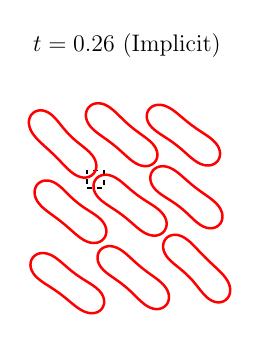
\begin{tikzpicture}[scale=0.6]

\begin{axis}[
  xmin = 0,
  xmax = 3.14,
  ymin = 0,
  ymax = 3.14,
  axis equal = true,
  hide axis,
  title = {\Large$t=0.26$ (Implicit)}
  ]

\addplot [mark=none,black,line width=1.0,dashed] table{
  1.1 1.8
  1.3 1.8
  1.3 2.0
  1.1 2.0
  1.1 1.8
};

\addplot [mark=none,red,line width=1.5] table{
1.2661e+00 3.7690e-01
1.2773e+00 3.8990e-01
1.2874e+00 4.0548e-01
1.2959e+00 4.2457e-01
1.3019e+00 4.4760e-01
1.3037e+00 4.7443e-01
1.2998e+00 5.0429e-01
1.2891e+00 5.3594e-01
1.2711e+00 5.6787e-01
1.2460e+00 5.9878e-01
1.2148e+00 6.2792e-01
1.1788e+00 6.5529e-01
1.1394e+00 6.8152e-01
1.0978e+00 7.0749e-01
1.0553e+00 7.3412e-01
1.0126e+00 7.6205e-01
9.7065e-01 7.9157e-01
9.2987e-01 8.2262e-01
8.9055e-01 8.5476e-01
8.5271e-01 8.8730e-01
8.1607e-01 9.1929e-01
7.8021e-01 9.4962e-01
7.4467e-01 9.7705e-01
7.0918e-01 1.0004e+00
6.7387e-01 1.0185e+00
6.3932e-01 1.0308e+00
6.0643e-01 1.0371e+00
5.7623e-01 1.0378e+00
5.4954e-01 1.0339e+00
5.2683e-01 1.0266e+00
5.0811e-01 1.0172e+00
4.9287e-01 1.0066e+00
4.8021e-01 9.9507e-01
4.6915e-01 9.8196e-01
4.5923e-01 9.6631e-01
4.5079e-01 9.4721e-01
4.4491e-01 9.2418e-01
4.4305e-01 8.9737e-01
4.4670e-01 8.6747e-01
4.5700e-01 8.3569e-01
4.7446e-01 8.0345e-01
4.9884e-01 7.7204e-01
5.2926e-01 7.4221e-01
5.6450e-01 7.1403e-01
6.0325e-01 6.8699e-01
6.4428e-01 6.6031e-01
6.8650e-01 6.3319e-01
7.2899e-01 6.0504e-01
7.7101e-01 5.7557e-01
8.1206e-01 5.4487e-01
8.5186e-01 5.1331e-01
8.9035e-01 4.8155e-01
9.2772e-01 4.5045e-01
9.6431e-01 4.2107e-01
1.0005e+00 3.9451e-01
1.0364e+00 3.7192e-01
1.0719e+00 3.5427e-01
1.1066e+00 3.4224e-01
1.1395e+00 3.3602e-01
1.1697e+00 3.3520e-01
1.1964e+00 3.3890e-01
1.2191e+00 3.4593e-01
1.2379e+00 3.5509e-01
1.2533e+00 3.6548e-01
1.2661e+00 3.7690e-01
};

\addplot [mark=none,red,line width=1.5] table{
2.0316e+00 4.3609e-01
2.0412e+00 4.5027e-01
2.0495e+00 4.6680e-01
2.0561e+00 4.8657e-01
2.0600e+00 5.0996e-01
2.0600e+00 5.3680e-01
2.0547e+00 5.6643e-01
2.0433e+00 5.9784e-01
2.0253e+00 6.2982e-01
2.0010e+00 6.6134e-01
1.9712e+00 6.9178e-01
1.9369e+00 7.2108e-01
1.8994e+00 7.4968e-01
1.8597e+00 7.7825e-01
1.8190e+00 8.0750e-01
1.7782e+00 8.3789e-01
1.7380e+00 8.6964e-01
1.6987e+00 9.0260e-01
1.6608e+00 9.3631e-01
1.6240e+00 9.7006e-01
1.5881e+00 1.0029e+00
1.5527e+00 1.0337e+00
1.5173e+00 1.0613e+00
1.4816e+00 1.0843e+00
1.4460e+00 1.1018e+00
1.4111e+00 1.1131e+00
1.3780e+00 1.1180e+00
1.3477e+00 1.1171e+00
1.3212e+00 1.1115e+00
1.2990e+00 1.1026e+00
1.2810e+00 1.0918e+00
1.2666e+00 1.0799e+00
1.2550e+00 1.0673e+00
1.2451e+00 1.0533e+00
1.2366e+00 1.0368e+00
1.2299e+00 1.0171e+00
1.2261e+00 9.9364e-01
1.2265e+00 9.6681e-01
1.2324e+00 9.3731e-01
1.2449e+00 9.0631e-01
1.2642e+00 8.7510e-01
1.2899e+00 8.4471e-01
1.3212e+00 8.1564e-01
1.3567e+00 7.8770e-01
1.3952e+00 7.6024e-01
1.4354e+00 7.3240e-01
1.4762e+00 7.0342e-01
1.5169e+00 6.7282e-01
1.5566e+00 6.4047e-01
1.5951e+00 6.0661e-01
1.6320e+00 5.7177e-01
1.6676e+00 5.3678e-01
1.7023e+00 5.0267e-01
1.7366e+00 4.7064e-01
1.7712e+00 4.4200e-01
1.8062e+00 4.1806e-01
1.8416e+00 3.9995e-01
1.8764e+00 3.8841e-01
1.9095e+00 3.8352e-01
1.9398e+00 3.8465e-01
1.9662e+00 3.9061e-01
1.9882e+00 3.9990e-01
2.0060e+00 4.1111e-01
2.0202e+00 4.2325e-01
2.0316e+00 4.3609e-01
};

\addplot [mark=none,red,line width=1.5] table{
2.7465e+00 5.1482e-01
2.7559e+00 5.2916e-01
2.7639e+00 5.4579e-01
2.7703e+00 5.6560e-01
2.7743e+00 5.8898e-01
2.7746e+00 6.1583e-01
2.7702e+00 6.4563e-01
2.7603e+00 6.7757e-01
2.7446e+00 7.1072e-01
2.7234e+00 7.4424e-01
2.6971e+00 7.7764e-01
2.6668e+00 8.1078e-01
2.6334e+00 8.4385e-01
2.5979e+00 8.7720e-01
2.5613e+00 9.1117e-01
2.5243e+00 9.4599e-01
2.4876e+00 9.8168e-01
2.4515e+00 1.0181e+00
2.4164e+00 1.0547e+00
2.3820e+00 1.0910e+00
2.3483e+00 1.1260e+00
2.3146e+00 1.1588e+00
2.2807e+00 1.1882e+00
2.2462e+00 1.2130e+00
2.2113e+00 1.2320e+00
2.1768e+00 1.2446e+00
2.1438e+00 1.2504e+00
2.1136e+00 1.2502e+00
2.0871e+00 1.2450e+00
2.0649e+00 1.2364e+00
2.0468e+00 1.2256e+00
2.0325e+00 1.2138e+00
2.0208e+00 1.2011e+00
2.0110e+00 1.1871e+00
2.0026e+00 1.1706e+00
1.9959e+00 1.1509e+00
1.9919e+00 1.1275e+00
1.9921e+00 1.1007e+00
1.9975e+00 1.0710e+00
2.0091e+00 1.0397e+00
2.0271e+00 1.0078e+00
2.0514e+00 9.7630e-01
2.0809e+00 9.4560e-01
2.1145e+00 9.1560e-01
2.1509e+00 8.8571e-01
2.1889e+00 8.5512e-01
2.2273e+00 8.2310e-01
2.2651e+00 7.8917e-01
2.3016e+00 7.5321e-01
2.3363e+00 7.1551e-01
2.3691e+00 6.7665e-01
2.4002e+00 6.3754e-01
2.4305e+00 5.9929e-01
2.4608e+00 5.6319e-01
2.4919e+00 5.3068e-01
2.5244e+00 5.0326e-01
2.5581e+00 4.8226e-01
2.5921e+00 4.6857e-01
2.6250e+00 4.6231e-01
2.6552e+00 4.6277e-01
2.6816e+00 4.6854e-01
2.7037e+00 4.7795e-01
2.7213e+00 4.8938e-01
2.7353e+00 5.0176e-01
2.7465e+00 5.1482e-01
};

\addplot [mark=none,red,line width=1.5] table{
1.2983e+00 1.2051e+00
1.3084e+00 1.2190e+00
1.3172e+00 1.2353e+00
1.3243e+00 1.2550e+00
1.3286e+00 1.2783e+00
1.3288e+00 1.3052e+00
1.3234e+00 1.3348e+00
1.3114e+00 1.3660e+00
1.2923e+00 1.3973e+00
1.2665e+00 1.4277e+00
1.2350e+00 1.4564e+00
1.1988e+00 1.4836e+00
1.1595e+00 1.5099e+00
1.1182e+00 1.5363e+00
1.0762e+00 1.5636e+00
1.0343e+00 1.5927e+00
9.9350e-01 1.6237e+00
9.5423e-01 1.6566e+00
9.1677e-01 1.6909e+00
8.8103e-01 1.7257e+00
8.4659e-01 1.7601e+00
8.1278e-01 1.7928e+00
7.7890e-01 1.8224e+00
7.4452e-01 1.8474e+00
7.0971e-01 1.8665e+00
6.7520e-01 1.8790e+00
6.4219e-01 1.8845e+00
6.1195e-01 1.8839e+00
5.8550e-01 1.8782e+00
5.6337e-01 1.8690e+00
5.4553e-01 1.8578e+00
5.3137e-01 1.8457e+00
5.1996e-01 1.8328e+00
5.1033e-01 1.8186e+00
5.0206e-01 1.8021e+00
4.9550e-01 1.7824e+00
4.9159e-01 1.7590e+00
4.9161e-01 1.7321e+00
4.9677e-01 1.7025e+00
5.0798e-01 1.6710e+00
5.2563e-01 1.6389e+00
5.4949e-01 1.6071e+00
5.7883e-01 1.5762e+00
6.1261e-01 1.5465e+00
6.4968e-01 1.5173e+00
6.8895e-01 1.4883e+00
7.2940e-01 1.4588e+00
7.7015e-01 1.4283e+00
8.1053e-01 1.3967e+00
8.5006e-01 1.3641e+00
8.8849e-01 1.3309e+00
9.2586e-01 1.2979e+00
9.6240e-01 1.2658e+00
9.9852e-01 1.2358e+00
1.0346e+00 1.2091e+00
1.0707e+00 1.1868e+00
1.1067e+00 1.1700e+00
1.1418e+00 1.1593e+00
1.1750e+00 1.1548e+00
1.2053e+00 1.1558e+00
1.2317e+00 1.1615e+00
1.2540e+00 1.1703e+00
1.2720e+00 1.1810e+00
1.2865e+00 1.1927e+00
1.2983e+00 1.2051e+00
};

\addplot [mark=none,red,line width=1.5] table{
2.0046e+00 1.2941e+00
2.0142e+00 1.3083e+00
2.0224e+00 1.3249e+00
2.0288e+00 1.3447e+00
2.0325e+00 1.3681e+00
2.0320e+00 1.3950e+00
2.0261e+00 1.4245e+00
2.0138e+00 1.4555e+00
1.9947e+00 1.4868e+00
1.9691e+00 1.5173e+00
1.9378e+00 1.5462e+00
1.9020e+00 1.5737e+00
1.8628e+00 1.6003e+00
1.8216e+00 1.6266e+00
1.7793e+00 1.6537e+00
1.7369e+00 1.6820e+00
1.6951e+00 1.7117e+00
1.6544e+00 1.7429e+00
1.6151e+00 1.7751e+00
1.5773e+00 1.8076e+00
1.5405e+00 1.8395e+00
1.5045e+00 1.8696e+00
1.4686e+00 1.8966e+00
1.4327e+00 1.9192e+00
1.3969e+00 1.9364e+00
1.3619e+00 1.9473e+00
1.3287e+00 1.9519e+00
1.2984e+00 1.9507e+00
1.2720e+00 1.9448e+00
1.2500e+00 1.9355e+00
1.2321e+00 1.9244e+00
1.2180e+00 1.9123e+00
1.2066e+00 1.8994e+00
1.1970e+00 1.8852e+00
1.1888e+00 1.8686e+00
1.1825e+00 1.8488e+00
1.1790e+00 1.8253e+00
1.1798e+00 1.7985e+00
1.1860e+00 1.7691e+00
1.1987e+00 1.7382e+00
1.2181e+00 1.7071e+00
1.2440e+00 1.6768e+00
1.2754e+00 1.6479e+00
1.3112e+00 1.6204e+00
1.3502e+00 1.5936e+00
1.3911e+00 1.5668e+00
1.4330e+00 1.5392e+00
1.4750e+00 1.5104e+00
1.5164e+00 1.4800e+00
1.5566e+00 1.4483e+00
1.5956e+00 1.4157e+00
1.6333e+00 1.3830e+00
1.6699e+00 1.3511e+00
1.7061e+00 1.3211e+00
1.7421e+00 1.2943e+00
1.7782e+00 1.2720e+00
1.8142e+00 1.2553e+00
1.8494e+00 1.2448e+00
1.8827e+00 1.2406e+00
1.9129e+00 1.2422e+00
1.9393e+00 1.2484e+00
1.9613e+00 1.2578e+00
1.9791e+00 1.2691e+00
1.9932e+00 1.2812e+00
2.0046e+00 1.2941e+00
};

\addplot [mark=none,red,line width=1.5] table{
2.6548e+00 1.3770e+00
2.6647e+00 1.3911e+00
2.6731e+00 1.4075e+00
2.6799e+00 1.4272e+00
2.6840e+00 1.4506e+00
2.6842e+00 1.4774e+00
2.6791e+00 1.5071e+00
2.6678e+00 1.5385e+00
2.6500e+00 1.5706e+00
2.6258e+00 1.6021e+00
2.5960e+00 1.6325e+00
2.5618e+00 1.6618e+00
2.5241e+00 1.6903e+00
2.4843e+00 1.7186e+00
2.4433e+00 1.7474e+00
2.4020e+00 1.7772e+00
2.3612e+00 1.8083e+00
2.3214e+00 1.8405e+00
2.2827e+00 1.8734e+00
2.2453e+00 1.9065e+00
2.2089e+00 1.9387e+00
2.1730e+00 1.9689e+00
2.1371e+00 1.9959e+00
2.1011e+00 2.0185e+00
2.0653e+00 2.0356e+00
2.0303e+00 2.0465e+00
1.9971e+00 2.0512e+00
1.9668e+00 2.0503e+00
1.9403e+00 2.0447e+00
1.9181e+00 2.0360e+00
1.9000e+00 2.0253e+00
1.8855e+00 2.0137e+00
1.8736e+00 2.0013e+00
1.8634e+00 1.9874e+00
1.8546e+00 1.9712e+00
1.8473e+00 1.9516e+00
1.8428e+00 1.9283e+00
1.8423e+00 1.9014e+00
1.8473e+00 1.8717e+00
1.8588e+00 1.8404e+00
1.8774e+00 1.8088e+00
1.9027e+00 1.7781e+00
1.9339e+00 1.7490e+00
1.9698e+00 1.7216e+00
2.0091e+00 1.6952e+00
2.0504e+00 1.6689e+00
2.0927e+00 1.6419e+00
2.1349e+00 1.6134e+00
2.1763e+00 1.5831e+00
2.2163e+00 1.5510e+00
2.2545e+00 1.5175e+00
2.2910e+00 1.4835e+00
2.3261e+00 1.4498e+00
2.3605e+00 1.4179e+00
2.3949e+00 1.3889e+00
2.4295e+00 1.3642e+00
2.4644e+00 1.3453e+00
2.4989e+00 1.3328e+00
2.5319e+00 1.3270e+00
2.5622e+00 1.3274e+00
2.5887e+00 1.3328e+00
2.6109e+00 1.3416e+00
2.6289e+00 1.3525e+00
2.6432e+00 1.3644e+00
2.6548e+00 1.3770e+00
};

\addplot [mark=none,red,line width=1.5] table{
1.1824e+00 1.9681e+00
1.1923e+00 1.9821e+00
1.2009e+00 1.9985e+00
1.2077e+00 2.0182e+00
1.2117e+00 2.0416e+00
1.2118e+00 2.0685e+00
1.2065e+00 2.0981e+00
1.1951e+00 2.1295e+00
1.1772e+00 2.1615e+00
1.1530e+00 2.1930e+00
1.1235e+00 2.2237e+00
1.0898e+00 2.2536e+00
1.0531e+00 2.2832e+00
1.0148e+00 2.3135e+00
9.7606e-01 2.3451e+00
9.3781e-01 2.3785e+00
9.0088e-01 2.4140e+00
8.6576e-01 2.4513e+00
8.3256e-01 2.4897e+00
8.0100e-01 2.5285e+00
7.7042e-01 2.5665e+00
7.3993e-01 2.6025e+00
7.0866e-01 2.6348e+00
6.7609e-01 2.6622e+00
6.4237e-01 2.6831e+00
6.0838e-01 2.6969e+00
5.7553e-01 2.7032e+00
5.4530e-01 2.7029e+00
5.1887e-01 2.6972e+00
4.9681e-01 2.6880e+00
4.7907e-01 2.6766e+00
4.6506e-01 2.6644e+00
4.5378e-01 2.6514e+00
4.4430e-01 2.6371e+00
4.3615e-01 2.6205e+00
4.2963e-01 2.6007e+00
4.2561e-01 2.5773e+00
4.2524e-01 2.5505e+00
4.2959e-01 2.5207e+00
4.3945e-01 2.4887e+00
4.5518e-01 2.4556e+00
4.7658e-01 2.4222e+00
5.0301e-01 2.3889e+00
5.3358e-01 2.3560e+00
5.6727e-01 2.3232e+00
6.0306e-01 2.2902e+00
6.4002e-01 2.2566e+00
6.7736e-01 2.2221e+00
7.1444e-01 2.1868e+00
7.5081e-01 2.1508e+00
7.8626e-01 2.1144e+00
8.2080e-01 2.0783e+00
8.5472e-01 2.0434e+00
8.8845e-01 2.0107e+00
9.2246e-01 1.9814e+00
9.5699e-01 1.9566e+00
9.9185e-01 1.9376e+00
1.0263e+00 1.9250e+00
1.0593e+00 1.9191e+00
1.0895e+00 1.9193e+00
1.1160e+00 1.9244e+00
1.1383e+00 1.9331e+00
1.1563e+00 1.9437e+00
1.1707e+00 1.9555e+00
1.1824e+00 1.9681e+00
};

\addplot [mark=none,red,line width=1.5] table{
1.8957e+00 2.1009e+00
1.9057e+00 2.1149e+00
1.9142e+00 2.1312e+00
1.9210e+00 2.1510e+00
1.9249e+00 2.1744e+00
1.9244e+00 2.2012e+00
1.9183e+00 2.2307e+00
1.9056e+00 2.2616e+00
1.8861e+00 2.2926e+00
1.8602e+00 2.3229e+00
1.8289e+00 2.3520e+00
1.7936e+00 2.3802e+00
1.7555e+00 2.4081e+00
1.7158e+00 2.4366e+00
1.6755e+00 2.4663e+00
1.6353e+00 2.4975e+00
1.5960e+00 2.5304e+00
1.5578e+00 2.5645e+00
1.5210e+00 2.5995e+00
1.4853e+00 2.6344e+00
1.4505e+00 2.6683e+00
1.4159e+00 2.7001e+00
1.3811e+00 2.7285e+00
1.3459e+00 2.7522e+00
1.3106e+00 2.7701e+00
1.2757e+00 2.7816e+00
1.2426e+00 2.7865e+00
1.2123e+00 2.7854e+00
1.1859e+00 2.7795e+00
1.1638e+00 2.7704e+00
1.1459e+00 2.7593e+00
1.1317e+00 2.7473e+00
1.1201e+00 2.7346e+00
1.1103e+00 2.7205e+00
1.1018e+00 2.7040e+00
1.0950e+00 2.6843e+00
1.0908e+00 2.6610e+00
1.0906e+00 2.6341e+00
1.0955e+00 2.6044e+00
1.1065e+00 2.5729e+00
1.1242e+00 2.5408e+00
1.1482e+00 2.5091e+00
1.1779e+00 2.4785e+00
1.2122e+00 2.4492e+00
1.2498e+00 2.4206e+00
1.2896e+00 2.3923e+00
1.3305e+00 2.3633e+00
1.3716e+00 2.3333e+00
1.4122e+00 2.3019e+00
1.4517e+00 2.2693e+00
1.4899e+00 2.2359e+00
1.5268e+00 2.2023e+00
1.5628e+00 2.1696e+00
1.5982e+00 2.1387e+00
1.6335e+00 2.1110e+00
1.6689e+00 2.0876e+00
1.7043e+00 2.0696e+00
1.7390e+00 2.0578e+00
1.7721e+00 2.0523e+00
1.8023e+00 2.0526e+00
1.8289e+00 2.0577e+00
1.8512e+00 2.0662e+00
1.8694e+00 2.0768e+00
1.8839e+00 2.0884e+00
1.8957e+00 2.1009e+00
};

\addplot [mark=none,red,line width=1.5] table{
2.6207e+00 2.1042e+00
2.6315e+00 2.1175e+00
2.6412e+00 2.1333e+00
2.6493e+00 2.1525e+00
2.6549e+00 2.1756e+00
2.6565e+00 2.2024e+00
2.6526e+00 2.2323e+00
2.6422e+00 2.2640e+00
2.6247e+00 2.2962e+00
2.6004e+00 2.3277e+00
2.5701e+00 2.3577e+00
2.5351e+00 2.3861e+00
2.4966e+00 2.4135e+00
2.4559e+00 2.4406e+00
2.4140e+00 2.4682e+00
2.3719e+00 2.4968e+00
2.3302e+00 2.5267e+00
2.2894e+00 2.5578e+00
2.2499e+00 2.5897e+00
2.2117e+00 2.6218e+00
2.1745e+00 2.6531e+00
2.1380e+00 2.6827e+00
2.1020e+00 2.7093e+00
2.0661e+00 2.7320e+00
2.0305e+00 2.7496e+00
1.9959e+00 2.7616e+00
1.9629e+00 2.7677e+00
1.9327e+00 2.7684e+00
1.9061e+00 2.7646e+00
1.8833e+00 2.7574e+00
1.8646e+00 2.7481e+00
1.8494e+00 2.7375e+00
1.8367e+00 2.7260e+00
1.8256e+00 2.7129e+00
1.8158e+00 2.6972e+00
1.8074e+00 2.6780e+00
1.8018e+00 2.6548e+00
1.8005e+00 2.6280e+00
1.8048e+00 2.5982e+00
1.8160e+00 2.5668e+00
1.8346e+00 2.5351e+00
1.8600e+00 2.5045e+00
1.8914e+00 2.4755e+00
1.9274e+00 2.4481e+00
1.9666e+00 2.4215e+00
2.0077e+00 2.3949e+00
2.0497e+00 2.3675e+00
2.0917e+00 2.3388e+00
2.1331e+00 2.3084e+00
2.1733e+00 2.2767e+00
2.2122e+00 2.2439e+00
2.2496e+00 2.2109e+00
2.2859e+00 2.1785e+00
2.3215e+00 2.1478e+00
2.3568e+00 2.1202e+00
2.3922e+00 2.0967e+00
2.4275e+00 2.0785e+00
2.4621e+00 2.0664e+00
2.4951e+00 2.0603e+00
2.5253e+00 2.0600e+00
2.5519e+00 2.0642e+00
2.5746e+00 2.0718e+00
2.5931e+00 2.0815e+00
2.6082e+00 2.0924e+00
2.6207e+00 2.1042e+00
};

\end{axis}

%\draw[gray,thin] (0,0) grid +(3,4);

\end{tikzpicture}

 \\
    &
    \begin{tikzpicture}[scale=0.6]

\begin{axis}[
  xmin = 1.1,
  xmax = 1.3,
  ymin = 1.8,
  ymax = 2.0,
  axis equal = true,
  hide axis,
  ]

\addplot [mark=none,red,line width=1.5] table{
1.2484e+00 3.5939e-01
1.2596e+00 3.7238e-01
1.2697e+00 3.8794e-01
1.2783e+00 4.0701e-01
1.2843e+00 4.3005e-01
1.2861e+00 4.5688e-01
1.2822e+00 4.8673e-01
1.2714e+00 5.1832e-01
1.2530e+00 5.5006e-01
1.2274e+00 5.8058e-01
1.1956e+00 6.0907e-01
1.1588e+00 6.3552e-01
1.1185e+00 6.6058e-01
1.0761e+00 6.8522e-01
1.0326e+00 7.1045e-01
9.8899e-01 7.3701e-01
9.4611e-01 7.6529e-01
9.0450e-01 7.9526e-01
8.6447e-01 8.2651e-01
8.2602e-01 8.5834e-01
7.8889e-01 8.8977e-01
7.5266e-01 9.1964e-01
7.1684e-01 9.4672e-01
6.8116e-01 9.6976e-01
6.4573e-01 9.8769e-01
6.1110e-01 9.9979e-01
5.7817e-01 1.0059e+00
5.4796e-01 1.0065e+00
5.2128e-01 1.0025e+00
4.9860e-01 9.9509e-01
4.7992e-01 9.8562e-01
4.6472e-01 9.7497e-01
4.5210e-01 9.6334e-01
4.4111e-01 9.5018e-01
4.3126e-01 9.3449e-01
4.2291e-01 9.1535e-01
4.1715e-01 8.9230e-01
4.1545e-01 8.6548e-01
4.1928e-01 8.3561e-01
4.2980e-01 8.0390e-01
4.4752e-01 7.7180e-01
4.7217e-01 7.4060e-01
5.0288e-01 7.1106e-01
5.3844e-01 6.8324e-01
5.7754e-01 6.5667e-01
6.1896e-01 6.3055e-01
6.6163e-01 6.0409e-01
7.0465e-01 5.7670e-01
7.4730e-01 5.4809e-01
7.8906e-01 5.1832e-01
8.2964e-01 4.8776e-01
8.6897e-01 4.5703e-01
9.0719e-01 4.2700e-01
9.4459e-01 3.9867e-01
9.8146e-01 3.7313e-01
1.0180e+00 3.5147e-01
1.0539e+00 3.3466e-01
1.0888e+00 3.2334e-01
1.1218e+00 3.1765e-01
1.1521e+00 3.1722e-01
1.1787e+00 3.2117e-01
1.2015e+00 3.2834e-01
1.2202e+00 3.3756e-01
1.2356e+00 3.4798e-01
1.2484e+00 3.5939e-01
};

\addplot [mark=none,red,line width=1.5] table{
2.0184e+00 4.4666e-01
2.0278e+00 4.6103e-01
2.0358e+00 4.7771e-01
2.0420e+00 4.9757e-01
2.0456e+00 5.2100e-01
2.0452e+00 5.4782e-01
2.0396e+00 5.7740e-01
2.0278e+00 6.0866e-01
2.0094e+00 6.4038e-01
1.9845e+00 6.7144e-01
1.9539e+00 7.0114e-01
1.9186e+00 7.2938e-01
1.8800e+00 7.5660e-01
1.8391e+00 7.8360e-01
1.7972e+00 8.1120e-01
1.7552e+00 8.4008e-01
1.7140e+00 8.7058e-01
1.6740e+00 9.0263e-01
1.6355e+00 9.3579e-01
1.5985e+00 9.6929e-01
1.5626e+00 1.0021e+00
1.5272e+00 1.0330e+00
1.4918e+00 1.0607e+00
1.4560e+00 1.0838e+00
1.4202e+00 1.1012e+00
1.3851e+00 1.1121e+00
1.3519e+00 1.1166e+00
1.3216e+00 1.1151e+00
1.2951e+00 1.1089e+00
1.2730e+00 1.0994e+00
1.2552e+00 1.0879e+00
1.2412e+00 1.0755e+00
1.2299e+00 1.0624e+00
1.2206e+00 1.0481e+00
1.2127e+00 1.0314e+00
1.2066e+00 1.0115e+00
1.2035e+00 9.8796e-01
1.2046e+00 9.6114e-01
1.2112e+00 9.3179e-01
1.2242e+00 9.0104e-01
1.2440e+00 8.7015e-01
1.2701e+00 8.4010e-01
1.3017e+00 8.1137e-01
1.3375e+00 7.8377e-01
1.3762e+00 7.5666e-01
1.4167e+00 7.2920e-01
1.4579e+00 7.0064e-01
1.4989e+00 6.7049e-01
1.5391e+00 6.3863e-01
1.5780e+00 6.0527e-01
1.6154e+00 5.7100e-01
1.6516e+00 5.3663e-01
1.6870e+00 5.0324e-01
1.7221e+00 4.7204e-01
1.7574e+00 4.4436e-01
1.7931e+00 4.2150e-01
1.8290e+00 4.0456e-01
1.8642e+00 3.9419e-01
1.8976e+00 3.9043e-01
1.9278e+00 3.9256e-01
1.9541e+00 3.9937e-01
1.9759e+00 4.0933e-01
1.9934e+00 4.2105e-01
2.0073e+00 4.3355e-01
2.0184e+00 4.4666e-01
};

\addplot [mark=none,red,line width=1.5] table{
2.7136e+00 5.5896e-01
2.7231e+00 5.7318e-01
2.7314e+00 5.8973e-01
2.7380e+00 6.0946e-01
2.7422e+00 6.3281e-01
2.7429e+00 6.5966e-01
2.7388e+00 6.8953e-01
2.7293e+00 7.2159e-01
2.7140e+00 7.5490e-01
2.6931e+00 7.8861e-01
2.6671e+00 8.2221e-01
2.6370e+00 8.5552e-01
2.6037e+00 8.8871e-01
2.5683e+00 9.2207e-01
2.5316e+00 9.5594e-01
2.4944e+00 9.9053e-01
2.4573e+00 1.0259e+00
2.4209e+00 1.0619e+00
2.3853e+00 1.0981e+00
2.3506e+00 1.1341e+00
2.3167e+00 1.1689e+00
2.2831e+00 1.2018e+00
2.2493e+00 1.2315e+00
2.2153e+00 1.2569e+00
2.1809e+00 1.2770e+00
2.1468e+00 1.2907e+00
2.1141e+00 1.2979e+00
2.0839e+00 1.2990e+00
2.0573e+00 1.2949e+00
2.0349e+00 1.2870e+00
2.0166e+00 1.2766e+00
2.0021e+00 1.2649e+00
1.9904e+00 1.2522e+00
1.9808e+00 1.2381e+00
1.9727e+00 1.2215e+00
1.9665e+00 1.2017e+00
1.9631e+00 1.1783e+00
1.9639e+00 1.1514e+00
1.9697e+00 1.1219e+00
1.9815e+00 1.0907e+00
1.9994e+00 1.0587e+00
2.0231e+00 1.0268e+00
2.0517e+00 9.9543e-01
2.0843e+00 9.6444e-01
2.1197e+00 9.3341e-01
2.1567e+00 9.0169e-01
2.1943e+00 8.6872e-01
2.2314e+00 8.3408e-01
2.2675e+00 7.9770e-01
2.3019e+00 7.5980e-01
2.3347e+00 7.2093e-01
2.3660e+00 6.8193e-01
2.3965e+00 6.4386e-01
2.4270e+00 6.0796e-01
2.4584e+00 5.7565e-01
2.4910e+00 5.4838e-01
2.5247e+00 5.2746e-01
2.5587e+00 5.1377e-01
2.5916e+00 5.0743e-01
2.6218e+00 5.0774e-01
2.6483e+00 5.1333e-01
2.6704e+00 5.2254e-01
2.6881e+00 5.3380e-01
2.7022e+00 5.4603e-01
2.7136e+00 5.5896e-01
};

\addplot [mark=none,red,line width=1.5] table{
1.2873e+00 1.1774e+00
1.2975e+00 1.1912e+00
1.3065e+00 1.2073e+00
1.3140e+00 1.2268e+00
1.3188e+00 1.2501e+00
1.3197e+00 1.2770e+00
1.3151e+00 1.3068e+00
1.3040e+00 1.3383e+00
1.2857e+00 1.3700e+00
1.2603e+00 1.4007e+00
1.2288e+00 1.4294e+00
1.1922e+00 1.4559e+00
1.1519e+00 1.4810e+00
1.1094e+00 1.5055e+00
1.0659e+00 1.5307e+00
1.0226e+00 1.5577e+00
9.8042e-01 1.5870e+00
9.4023e-01 1.6188e+00
9.0239e-01 1.6526e+00
8.6682e-01 1.6877e+00
8.3297e-01 1.7227e+00
8.0000e-01 1.7563e+00
7.6697e-01 1.7869e+00
7.3329e-01 1.8129e+00
6.9898e-01 1.8329e+00
6.6475e-01 1.8460e+00
6.3184e-01 1.8521e+00
6.0160e-01 1.8517e+00
5.7509e-01 1.8463e+00
5.5287e-01 1.8373e+00
5.3491e-01 1.8263e+00
5.2064e-01 1.8143e+00
5.0910e-01 1.8016e+00
4.9931e-01 1.7875e+00
4.9084e-01 1.7711e+00
4.8400e-01 1.7514e+00
4.7973e-01 1.7281e+00
4.7928e-01 1.7012e+00
4.8390e-01 1.6715e+00
4.9451e-01 1.6398e+00
5.1156e-01 1.6073e+00
5.3488e-01 1.5751e+00
5.6378e-01 1.5439e+00
5.9726e-01 1.5138e+00
6.3421e-01 1.4845e+00
6.7351e-01 1.4555e+00
7.1413e-01 1.4262e+00
7.5520e-01 1.3961e+00
7.9598e-01 1.3650e+00
8.3595e-01 1.3330e+00
8.7483e-01 1.3003e+00
9.1261e-01 1.2677e+00
9.4952e-01 1.2360e+00
9.8596e-01 1.2064e+00
1.0223e+00 1.1800e+00
1.0587e+00 1.1580e+00
1.0949e+00 1.1414e+00
1.1302e+00 1.1310e+00
1.1635e+00 1.1267e+00
1.1938e+00 1.1279e+00
1.2203e+00 1.1336e+00
1.2426e+00 1.1425e+00
1.2608e+00 1.1533e+00
1.2754e+00 1.1650e+00
1.2873e+00 1.1774e+00
};

\addplot [mark=none,red,line width=1.5] table{
1.9984e+00 1.2975e+00
2.0080e+00 1.3117e+00
2.0161e+00 1.3282e+00
2.0225e+00 1.3480e+00
2.0261e+00 1.3714e+00
2.0256e+00 1.3982e+00
2.0201e+00 1.4278e+00
2.0084e+00 1.4591e+00
1.9902e+00 1.4909e+00
1.9657e+00 1.5222e+00
1.9355e+00 1.5522e+00
1.9006e+00 1.5806e+00
1.8619e+00 1.6078e+00
1.8207e+00 1.6342e+00
1.7780e+00 1.6606e+00
1.7347e+00 1.6876e+00
1.6916e+00 1.7156e+00
1.6495e+00 1.7449e+00
1.6087e+00 1.7752e+00
1.5694e+00 1.8060e+00
1.5316e+00 1.8365e+00
1.4948e+00 1.8657e+00
1.4586e+00 1.8923e+00
1.4228e+00 1.9151e+00
1.3874e+00 1.9330e+00
1.3527e+00 1.9452e+00
1.3198e+00 1.9513e+00
1.2896e+00 1.9519e+00
1.2630e+00 1.9477e+00
1.2406e+00 1.9399e+00
1.2223e+00 1.9297e+00
1.2077e+00 1.9182e+00
1.1960e+00 1.9055e+00
1.1864e+00 1.8913e+00
1.1785e+00 1.8747e+00
1.1725e+00 1.8548e+00
1.1696e+00 1.8314e+00
1.1708e+00 1.8046e+00
1.1774e+00 1.7752e+00
1.1900e+00 1.7443e+00
1.2091e+00 1.7130e+00
1.2342e+00 1.6822e+00
1.2647e+00 1.6525e+00
1.2997e+00 1.6241e+00
1.3381e+00 1.5965e+00
1.3787e+00 1.5693e+00
1.4207e+00 1.5417e+00
1.4630e+00 1.5134e+00
1.5051e+00 1.4840e+00
1.5463e+00 1.4535e+00
1.5863e+00 1.4222e+00
1.6250e+00 1.3907e+00
1.6625e+00 1.3597e+00
1.6992e+00 1.3304e+00
1.7355e+00 1.3040e+00
1.7715e+00 1.2816e+00
1.8073e+00 1.2643e+00
1.8423e+00 1.2529e+00
1.8754e+00 1.2477e+00
1.9057e+00 1.2482e+00
1.9321e+00 1.2534e+00
1.9544e+00 1.2620e+00
1.9725e+00 1.2728e+00
1.9868e+00 1.2847e+00
1.9984e+00 1.2975e+00
};

\addplot [mark=none,red,line width=1.5] table{
2.6562e+00 1.4101e+00
2.6665e+00 1.4237e+00
2.6756e+00 1.4399e+00
2.6831e+00 1.4593e+00
2.6879e+00 1.4826e+00
2.6889e+00 1.5094e+00
2.6846e+00 1.5393e+00
2.6740e+00 1.5710e+00
2.6567e+00 1.6033e+00
2.6329e+00 1.6351e+00
2.6033e+00 1.6657e+00
2.5690e+00 1.6949e+00
2.5311e+00 1.7230e+00
2.4908e+00 1.7508e+00
2.4493e+00 1.7789e+00
2.4075e+00 1.8079e+00
2.3661e+00 1.8383e+00
2.3258e+00 1.8699e+00
2.2869e+00 1.9026e+00
2.2495e+00 1.9356e+00
2.2132e+00 1.9680e+00
2.1776e+00 1.9987e+00
2.1423e+00 2.0265e+00
2.1068e+00 2.0501e+00
2.0714e+00 2.0683e+00
2.0366e+00 2.0804e+00
2.0036e+00 2.0862e+00
1.9734e+00 2.0863e+00
1.9468e+00 2.0816e+00
1.9242e+00 2.0734e+00
1.9058e+00 2.0630e+00
1.8910e+00 2.0515e+00
1.8790e+00 2.0391e+00
1.8688e+00 2.0254e+00
1.8598e+00 2.0093e+00
1.8523e+00 1.9898e+00
1.8473e+00 1.9666e+00
1.8461e+00 1.9397e+00
1.8500e+00 1.9098e+00
1.8601e+00 1.8780e+00
1.8770e+00 1.8455e+00
1.9007e+00 1.8136e+00
1.9305e+00 1.7833e+00
1.9654e+00 1.7548e+00
2.0043e+00 1.7278e+00
2.0457e+00 1.7018e+00
2.0886e+00 1.6756e+00
2.1318e+00 1.6484e+00
2.1744e+00 1.6197e+00
2.2155e+00 1.5891e+00
2.2548e+00 1.5569e+00
2.2920e+00 1.5237e+00
2.3275e+00 1.4904e+00
2.3620e+00 1.4585e+00
2.3961e+00 1.4291e+00
2.4304e+00 1.4039e+00
2.4649e+00 1.3842e+00
2.4990e+00 1.3709e+00
2.5318e+00 1.3642e+00
2.5620e+00 1.3637e+00
2.5886e+00 1.3681e+00
2.6111e+00 1.3762e+00
2.6295e+00 1.3864e+00
2.6442e+00 1.3978e+00
2.6562e+00 1.4101e+00
};

\addplot [mark=none,red,line width=1.5] table{
1.2108e+00 1.9141e+00
1.2207e+00 1.9281e+00
1.2288e+00 1.9446e+00
1.2351e+00 1.9644e+00
1.2385e+00 1.9878e+00
1.2378e+00 2.0146e+00
1.2321e+00 2.0442e+00
1.2207e+00 2.0755e+00
1.2032e+00 2.1077e+00
1.1800e+00 2.1400e+00
1.1518e+00 2.1718e+00
1.1197e+00 2.2031e+00
1.0845e+00 2.2345e+00
1.0477e+00 2.2663e+00
1.0101e+00 2.2993e+00
9.7274e-01 2.3337e+00
9.3638e-01 2.3698e+00
9.0155e-01 2.4073e+00
8.6838e-01 2.4458e+00
8.3671e-01 2.4845e+00
8.0592e-01 2.5224e+00
7.7523e-01 2.5581e+00
7.4382e-01 2.5904e+00
7.1122e-01 2.6177e+00
6.7755e-01 2.6387e+00
6.4366e-01 2.6527e+00
6.1087e-01 2.6594e+00
5.8067e-01 2.6594e+00
5.5415e-01 2.6543e+00
5.3193e-01 2.6454e+00
5.1396e-01 2.6345e+00
4.9968e-01 2.6226e+00
4.8810e-01 2.6099e+00
4.7828e-01 2.5958e+00
4.6971e-01 2.5794e+00
4.6271e-01 2.5598e+00
4.5812e-01 2.5365e+00
4.5712e-01 2.5096e+00
4.6081e-01 2.4797e+00
4.7003e-01 2.4476e+00
4.8514e-01 2.4142e+00
5.0599e-01 2.3804e+00
5.3196e-01 2.3468e+00
5.6218e-01 2.3136e+00
5.9563e-01 2.2806e+00
6.3131e-01 2.2474e+00
6.6827e-01 2.2138e+00
7.0572e-01 2.1795e+00
7.4299e-01 2.1444e+00
7.7964e-01 2.1086e+00
8.1539e-01 2.0725e+00
8.5020e-01 2.0367e+00
8.8426e-01 2.0020e+00
9.1795e-01 1.9692e+00
9.5165e-01 1.9395e+00
9.8566e-01 1.9140e+00
1.0199e+00 1.8937e+00
1.0537e+00 1.8796e+00
1.0863e+00 1.8718e+00
1.1164e+00 1.8701e+00
1.1431e+00 1.8734e+00
1.1657e+00 1.8806e+00
1.1842e+00 1.8903e+00
1.1990e+00 1.9016e+00
1.2108e+00 1.9141e+00
};

\addplot [mark=none,red,line width=1.5] table{
1.9228e+00 2.0974e+00
1.9323e+00 2.1116e+00
1.9403e+00 2.1282e+00
1.9465e+00 2.1481e+00
1.9497e+00 2.1715e+00
1.9487e+00 2.1984e+00
1.9422e+00 2.2278e+00
1.9295e+00 2.2586e+00
1.9101e+00 2.2898e+00
1.8846e+00 2.3203e+00
1.8538e+00 2.3497e+00
1.8189e+00 2.3783e+00
1.7811e+00 2.4066e+00
1.7415e+00 2.4353e+00
1.7012e+00 2.4651e+00
1.6610e+00 2.4962e+00
1.6214e+00 2.5288e+00
1.5829e+00 2.5626e+00
1.5455e+00 2.5970e+00
1.5092e+00 2.6312e+00
1.4736e+00 2.6643e+00
1.4382e+00 2.6952e+00
1.4026e+00 2.7225e+00
1.3667e+00 2.7451e+00
1.3308e+00 2.7619e+00
1.2956e+00 2.7723e+00
1.2623e+00 2.7762e+00
1.2320e+00 2.7744e+00
1.2057e+00 2.7680e+00
1.1837e+00 2.7585e+00
1.1659e+00 2.7472e+00
1.1518e+00 2.7351e+00
1.1403e+00 2.7223e+00
1.1305e+00 2.7082e+00
1.1220e+00 2.6918e+00
1.1150e+00 2.6722e+00
1.1106e+00 2.6488e+00
1.1101e+00 2.6220e+00
1.1147e+00 2.5922e+00
1.1256e+00 2.5606e+00
1.1431e+00 2.5284e+00
1.1673e+00 2.4969e+00
1.1975e+00 2.4668e+00
1.2326e+00 2.4384e+00
1.2714e+00 2.4113e+00
1.3126e+00 2.3849e+00
1.3551e+00 2.3581e+00
1.3978e+00 2.3302e+00
1.4398e+00 2.3006e+00
1.4804e+00 2.2694e+00
1.5193e+00 2.2367e+00
1.5565e+00 2.2034e+00
1.5922e+00 2.1704e+00
1.6272e+00 2.1390e+00
1.6619e+00 2.1104e+00
1.6968e+00 2.0860e+00
1.7318e+00 2.0672e+00
1.7664e+00 2.0545e+00
1.7994e+00 2.0484e+00
1.8296e+00 2.0483e+00
1.8562e+00 2.0531e+00
1.8786e+00 2.0616e+00
1.8969e+00 2.0725e+00
1.9113e+00 2.0845e+00
1.9228e+00 2.0974e+00
};

\addplot [mark=none,red,line width=1.5] table{
2.6498e+00 2.1330e+00
2.6605e+00 2.1464e+00
2.6701e+00 2.1622e+00
2.6782e+00 2.1815e+00
2.6836e+00 2.2046e+00
2.6851e+00 2.2314e+00
2.6812e+00 2.2613e+00
2.6707e+00 2.2930e+00
2.6532e+00 2.3253e+00
2.6289e+00 2.3567e+00
2.5987e+00 2.3867e+00
2.5637e+00 2.4151e+00
2.5251e+00 2.4424e+00
2.4842e+00 2.4693e+00
2.4421e+00 2.4965e+00
2.3995e+00 2.5246e+00
2.3574e+00 2.5539e+00
2.3160e+00 2.5842e+00
2.2758e+00 2.6152e+00
2.2367e+00 2.6462e+00
2.1986e+00 2.6765e+00
2.1613e+00 2.7049e+00
2.1245e+00 2.7305e+00
2.0880e+00 2.7521e+00
2.0520e+00 2.7688e+00
2.0170e+00 2.7800e+00
1.9839e+00 2.7854e+00
1.9537e+00 2.7856e+00
1.9270e+00 2.7815e+00
1.9044e+00 2.7741e+00
1.8857e+00 2.7647e+00
1.8705e+00 2.7541e+00
1.8578e+00 2.7425e+00
1.8467e+00 2.7294e+00
1.8368e+00 2.7137e+00
1.8284e+00 2.6946e+00
1.8227e+00 2.6715e+00
1.8212e+00 2.6446e+00
1.8254e+00 2.6148e+00
1.8366e+00 2.5834e+00
1.8553e+00 2.5518e+00
1.8811e+00 2.5215e+00
1.9131e+00 2.4932e+00
1.9500e+00 2.4668e+00
1.9902e+00 2.4418e+00
2.0326e+00 2.4170e+00
2.0760e+00 2.3915e+00
2.1193e+00 2.3645e+00
2.1617e+00 2.3356e+00
2.2028e+00 2.3049e+00
2.2420e+00 2.2727e+00
2.2796e+00 2.2398e+00
2.3158e+00 2.2073e+00
2.3513e+00 2.1764e+00
2.3864e+00 2.1485e+00
2.4217e+00 2.1248e+00
2.4569e+00 2.1065e+00
2.4915e+00 2.0943e+00
2.5245e+00 2.0883e+00
2.5547e+00 2.0881e+00
2.5813e+00 2.0925e+00
2.6039e+00 2.1003e+00
2.6224e+00 2.1102e+00
2.6374e+00 2.1211e+00
2.6498e+00 2.1330e+00
};

\end{axis}

%\draw[gray,thin] (0,0) grid +(3,4);

\end{tikzpicture}

 &
    \begin{tikzpicture}[scale=0.6]

\begin{axis}[
  xmin = 1.1,
  xmax = 1.3,
  ymin = 1.8,
  ymax = 2.0,
  axis equal = true,
  hide axis,
  ]

\addplot [mark=none,red,line width=1.5] table{
1.2661e+00 3.7690e-01
1.2773e+00 3.8990e-01
1.2874e+00 4.0548e-01
1.2959e+00 4.2457e-01
1.3019e+00 4.4760e-01
1.3037e+00 4.7443e-01
1.2998e+00 5.0429e-01
1.2891e+00 5.3594e-01
1.2711e+00 5.6787e-01
1.2460e+00 5.9878e-01
1.2148e+00 6.2792e-01
1.1788e+00 6.5529e-01
1.1394e+00 6.8152e-01
1.0978e+00 7.0749e-01
1.0553e+00 7.3412e-01
1.0126e+00 7.6205e-01
9.7065e-01 7.9157e-01
9.2987e-01 8.2262e-01
8.9055e-01 8.5476e-01
8.5271e-01 8.8730e-01
8.1607e-01 9.1929e-01
7.8021e-01 9.4962e-01
7.4467e-01 9.7705e-01
7.0918e-01 1.0004e+00
6.7387e-01 1.0185e+00
6.3932e-01 1.0308e+00
6.0643e-01 1.0371e+00
5.7623e-01 1.0378e+00
5.4954e-01 1.0339e+00
5.2683e-01 1.0266e+00
5.0811e-01 1.0172e+00
4.9287e-01 1.0066e+00
4.8021e-01 9.9507e-01
4.6915e-01 9.8196e-01
4.5923e-01 9.6631e-01
4.5079e-01 9.4721e-01
4.4491e-01 9.2418e-01
4.4305e-01 8.9737e-01
4.4670e-01 8.6747e-01
4.5700e-01 8.3569e-01
4.7446e-01 8.0345e-01
4.9884e-01 7.7204e-01
5.2926e-01 7.4221e-01
5.6450e-01 7.1403e-01
6.0325e-01 6.8699e-01
6.4428e-01 6.6031e-01
6.8650e-01 6.3319e-01
7.2899e-01 6.0504e-01
7.7101e-01 5.7557e-01
8.1206e-01 5.4487e-01
8.5186e-01 5.1331e-01
8.9035e-01 4.8155e-01
9.2772e-01 4.5045e-01
9.6431e-01 4.2107e-01
1.0005e+00 3.9451e-01
1.0364e+00 3.7192e-01
1.0719e+00 3.5427e-01
1.1066e+00 3.4224e-01
1.1395e+00 3.3602e-01
1.1697e+00 3.3520e-01
1.1964e+00 3.3890e-01
1.2191e+00 3.4593e-01
1.2379e+00 3.5509e-01
1.2533e+00 3.6548e-01
1.2661e+00 3.7690e-01
};

\addplot [mark=none,red,line width=1.5] table{
2.0316e+00 4.3609e-01
2.0412e+00 4.5027e-01
2.0495e+00 4.6680e-01
2.0561e+00 4.8657e-01
2.0600e+00 5.0996e-01
2.0600e+00 5.3680e-01
2.0547e+00 5.6643e-01
2.0433e+00 5.9784e-01
2.0253e+00 6.2982e-01
2.0010e+00 6.6134e-01
1.9712e+00 6.9178e-01
1.9369e+00 7.2108e-01
1.8994e+00 7.4968e-01
1.8597e+00 7.7825e-01
1.8190e+00 8.0750e-01
1.7782e+00 8.3789e-01
1.7380e+00 8.6964e-01
1.6987e+00 9.0260e-01
1.6608e+00 9.3631e-01
1.6240e+00 9.7006e-01
1.5881e+00 1.0029e+00
1.5527e+00 1.0337e+00
1.5173e+00 1.0613e+00
1.4816e+00 1.0843e+00
1.4460e+00 1.1018e+00
1.4111e+00 1.1131e+00
1.3780e+00 1.1180e+00
1.3477e+00 1.1171e+00
1.3212e+00 1.1115e+00
1.2990e+00 1.1026e+00
1.2810e+00 1.0918e+00
1.2666e+00 1.0799e+00
1.2550e+00 1.0673e+00
1.2451e+00 1.0533e+00
1.2366e+00 1.0368e+00
1.2299e+00 1.0171e+00
1.2261e+00 9.9364e-01
1.2265e+00 9.6681e-01
1.2324e+00 9.3731e-01
1.2449e+00 9.0631e-01
1.2642e+00 8.7510e-01
1.2899e+00 8.4471e-01
1.3212e+00 8.1564e-01
1.3567e+00 7.8770e-01
1.3952e+00 7.6024e-01
1.4354e+00 7.3240e-01
1.4762e+00 7.0342e-01
1.5169e+00 6.7282e-01
1.5566e+00 6.4047e-01
1.5951e+00 6.0661e-01
1.6320e+00 5.7177e-01
1.6676e+00 5.3678e-01
1.7023e+00 5.0267e-01
1.7366e+00 4.7064e-01
1.7712e+00 4.4200e-01
1.8062e+00 4.1806e-01
1.8416e+00 3.9995e-01
1.8764e+00 3.8841e-01
1.9095e+00 3.8352e-01
1.9398e+00 3.8465e-01
1.9662e+00 3.9061e-01
1.9882e+00 3.9990e-01
2.0060e+00 4.1111e-01
2.0202e+00 4.2325e-01
2.0316e+00 4.3609e-01
};

\addplot [mark=none,red,line width=1.5] table{
2.7465e+00 5.1482e-01
2.7559e+00 5.2916e-01
2.7639e+00 5.4579e-01
2.7703e+00 5.6560e-01
2.7743e+00 5.8898e-01
2.7746e+00 6.1583e-01
2.7702e+00 6.4563e-01
2.7603e+00 6.7757e-01
2.7446e+00 7.1072e-01
2.7234e+00 7.4424e-01
2.6971e+00 7.7764e-01
2.6668e+00 8.1078e-01
2.6334e+00 8.4385e-01
2.5979e+00 8.7720e-01
2.5613e+00 9.1117e-01
2.5243e+00 9.4599e-01
2.4876e+00 9.8168e-01
2.4515e+00 1.0181e+00
2.4164e+00 1.0547e+00
2.3820e+00 1.0910e+00
2.3483e+00 1.1260e+00
2.3146e+00 1.1588e+00
2.2807e+00 1.1882e+00
2.2462e+00 1.2130e+00
2.2113e+00 1.2320e+00
2.1768e+00 1.2446e+00
2.1438e+00 1.2504e+00
2.1136e+00 1.2502e+00
2.0871e+00 1.2450e+00
2.0649e+00 1.2364e+00
2.0468e+00 1.2256e+00
2.0325e+00 1.2138e+00
2.0208e+00 1.2011e+00
2.0110e+00 1.1871e+00
2.0026e+00 1.1706e+00
1.9959e+00 1.1509e+00
1.9919e+00 1.1275e+00
1.9921e+00 1.1007e+00
1.9975e+00 1.0710e+00
2.0091e+00 1.0397e+00
2.0271e+00 1.0078e+00
2.0514e+00 9.7630e-01
2.0809e+00 9.4560e-01
2.1145e+00 9.1560e-01
2.1509e+00 8.8571e-01
2.1889e+00 8.5512e-01
2.2273e+00 8.2310e-01
2.2651e+00 7.8917e-01
2.3016e+00 7.5321e-01
2.3363e+00 7.1551e-01
2.3691e+00 6.7665e-01
2.4002e+00 6.3754e-01
2.4305e+00 5.9929e-01
2.4608e+00 5.6319e-01
2.4919e+00 5.3068e-01
2.5244e+00 5.0326e-01
2.5581e+00 4.8226e-01
2.5921e+00 4.6857e-01
2.6250e+00 4.6231e-01
2.6552e+00 4.6277e-01
2.6816e+00 4.6854e-01
2.7037e+00 4.7795e-01
2.7213e+00 4.8938e-01
2.7353e+00 5.0176e-01
2.7465e+00 5.1482e-01
};

\addplot [mark=none,red,line width=1.5] table{
1.2983e+00 1.2051e+00
1.3084e+00 1.2190e+00
1.3172e+00 1.2353e+00
1.3243e+00 1.2550e+00
1.3286e+00 1.2783e+00
1.3288e+00 1.3052e+00
1.3234e+00 1.3348e+00
1.3114e+00 1.3660e+00
1.2923e+00 1.3973e+00
1.2665e+00 1.4277e+00
1.2350e+00 1.4564e+00
1.1988e+00 1.4836e+00
1.1595e+00 1.5099e+00
1.1182e+00 1.5363e+00
1.0762e+00 1.5636e+00
1.0343e+00 1.5927e+00
9.9350e-01 1.6237e+00
9.5423e-01 1.6566e+00
9.1677e-01 1.6909e+00
8.8103e-01 1.7257e+00
8.4659e-01 1.7601e+00
8.1278e-01 1.7928e+00
7.7890e-01 1.8224e+00
7.4452e-01 1.8474e+00
7.0971e-01 1.8665e+00
6.7520e-01 1.8790e+00
6.4219e-01 1.8845e+00
6.1195e-01 1.8839e+00
5.8550e-01 1.8782e+00
5.6337e-01 1.8690e+00
5.4553e-01 1.8578e+00
5.3137e-01 1.8457e+00
5.1996e-01 1.8328e+00
5.1033e-01 1.8186e+00
5.0206e-01 1.8021e+00
4.9550e-01 1.7824e+00
4.9159e-01 1.7590e+00
4.9161e-01 1.7321e+00
4.9677e-01 1.7025e+00
5.0798e-01 1.6710e+00
5.2563e-01 1.6389e+00
5.4949e-01 1.6071e+00
5.7883e-01 1.5762e+00
6.1261e-01 1.5465e+00
6.4968e-01 1.5173e+00
6.8895e-01 1.4883e+00
7.2940e-01 1.4588e+00
7.7015e-01 1.4283e+00
8.1053e-01 1.3967e+00
8.5006e-01 1.3641e+00
8.8849e-01 1.3309e+00
9.2586e-01 1.2979e+00
9.6240e-01 1.2658e+00
9.9852e-01 1.2358e+00
1.0346e+00 1.2091e+00
1.0707e+00 1.1868e+00
1.1067e+00 1.1700e+00
1.1418e+00 1.1593e+00
1.1750e+00 1.1548e+00
1.2053e+00 1.1558e+00
1.2317e+00 1.1615e+00
1.2540e+00 1.1703e+00
1.2720e+00 1.1810e+00
1.2865e+00 1.1927e+00
1.2983e+00 1.2051e+00
};

\addplot [mark=none,red,line width=1.5] table{
2.0046e+00 1.2941e+00
2.0142e+00 1.3083e+00
2.0224e+00 1.3249e+00
2.0288e+00 1.3447e+00
2.0325e+00 1.3681e+00
2.0320e+00 1.3950e+00
2.0261e+00 1.4245e+00
2.0138e+00 1.4555e+00
1.9947e+00 1.4868e+00
1.9691e+00 1.5173e+00
1.9378e+00 1.5462e+00
1.9020e+00 1.5737e+00
1.8628e+00 1.6003e+00
1.8216e+00 1.6266e+00
1.7793e+00 1.6537e+00
1.7369e+00 1.6820e+00
1.6951e+00 1.7117e+00
1.6544e+00 1.7429e+00
1.6151e+00 1.7751e+00
1.5773e+00 1.8076e+00
1.5405e+00 1.8395e+00
1.5045e+00 1.8696e+00
1.4686e+00 1.8966e+00
1.4327e+00 1.9192e+00
1.3969e+00 1.9364e+00
1.3619e+00 1.9473e+00
1.3287e+00 1.9519e+00
1.2984e+00 1.9507e+00
1.2720e+00 1.9448e+00
1.2500e+00 1.9355e+00
1.2321e+00 1.9244e+00
1.2180e+00 1.9123e+00
1.2066e+00 1.8994e+00
1.1970e+00 1.8852e+00
1.1888e+00 1.8686e+00
1.1825e+00 1.8488e+00
1.1790e+00 1.8253e+00
1.1798e+00 1.7985e+00
1.1860e+00 1.7691e+00
1.1987e+00 1.7382e+00
1.2181e+00 1.7071e+00
1.2440e+00 1.6768e+00
1.2754e+00 1.6479e+00
1.3112e+00 1.6204e+00
1.3502e+00 1.5936e+00
1.3911e+00 1.5668e+00
1.4330e+00 1.5392e+00
1.4750e+00 1.5104e+00
1.5164e+00 1.4800e+00
1.5566e+00 1.4483e+00
1.5956e+00 1.4157e+00
1.6333e+00 1.3830e+00
1.6699e+00 1.3511e+00
1.7061e+00 1.3211e+00
1.7421e+00 1.2943e+00
1.7782e+00 1.2720e+00
1.8142e+00 1.2553e+00
1.8494e+00 1.2448e+00
1.8827e+00 1.2406e+00
1.9129e+00 1.2422e+00
1.9393e+00 1.2484e+00
1.9613e+00 1.2578e+00
1.9791e+00 1.2691e+00
1.9932e+00 1.2812e+00
2.0046e+00 1.2941e+00
};

\addplot [mark=none,red,line width=1.5] table{
2.6548e+00 1.3770e+00
2.6647e+00 1.3911e+00
2.6731e+00 1.4075e+00
2.6799e+00 1.4272e+00
2.6840e+00 1.4506e+00
2.6842e+00 1.4774e+00
2.6791e+00 1.5071e+00
2.6678e+00 1.5385e+00
2.6500e+00 1.5706e+00
2.6258e+00 1.6021e+00
2.5960e+00 1.6325e+00
2.5618e+00 1.6618e+00
2.5241e+00 1.6903e+00
2.4843e+00 1.7186e+00
2.4433e+00 1.7474e+00
2.4020e+00 1.7772e+00
2.3612e+00 1.8083e+00
2.3214e+00 1.8405e+00
2.2827e+00 1.8734e+00
2.2453e+00 1.9065e+00
2.2089e+00 1.9387e+00
2.1730e+00 1.9689e+00
2.1371e+00 1.9959e+00
2.1011e+00 2.0185e+00
2.0653e+00 2.0356e+00
2.0303e+00 2.0465e+00
1.9971e+00 2.0512e+00
1.9668e+00 2.0503e+00
1.9403e+00 2.0447e+00
1.9181e+00 2.0360e+00
1.9000e+00 2.0253e+00
1.8855e+00 2.0137e+00
1.8736e+00 2.0013e+00
1.8634e+00 1.9874e+00
1.8546e+00 1.9712e+00
1.8473e+00 1.9516e+00
1.8428e+00 1.9283e+00
1.8423e+00 1.9014e+00
1.8473e+00 1.8717e+00
1.8588e+00 1.8404e+00
1.8774e+00 1.8088e+00
1.9027e+00 1.7781e+00
1.9339e+00 1.7490e+00
1.9698e+00 1.7216e+00
2.0091e+00 1.6952e+00
2.0504e+00 1.6689e+00
2.0927e+00 1.6419e+00
2.1349e+00 1.6134e+00
2.1763e+00 1.5831e+00
2.2163e+00 1.5510e+00
2.2545e+00 1.5175e+00
2.2910e+00 1.4835e+00
2.3261e+00 1.4498e+00
2.3605e+00 1.4179e+00
2.3949e+00 1.3889e+00
2.4295e+00 1.3642e+00
2.4644e+00 1.3453e+00
2.4989e+00 1.3328e+00
2.5319e+00 1.3270e+00
2.5622e+00 1.3274e+00
2.5887e+00 1.3328e+00
2.6109e+00 1.3416e+00
2.6289e+00 1.3525e+00
2.6432e+00 1.3644e+00
2.6548e+00 1.3770e+00
};

\addplot [mark=none,red,line width=1.5] table{
1.1824e+00 1.9681e+00
1.1923e+00 1.9821e+00
1.2009e+00 1.9985e+00
1.2077e+00 2.0182e+00
1.2117e+00 2.0416e+00
1.2118e+00 2.0685e+00
1.2065e+00 2.0981e+00
1.1951e+00 2.1295e+00
1.1772e+00 2.1615e+00
1.1530e+00 2.1930e+00
1.1235e+00 2.2237e+00
1.0898e+00 2.2536e+00
1.0531e+00 2.2832e+00
1.0148e+00 2.3135e+00
9.7606e-01 2.3451e+00
9.3781e-01 2.3785e+00
9.0088e-01 2.4140e+00
8.6576e-01 2.4513e+00
8.3256e-01 2.4897e+00
8.0100e-01 2.5285e+00
7.7042e-01 2.5665e+00
7.3993e-01 2.6025e+00
7.0866e-01 2.6348e+00
6.7609e-01 2.6622e+00
6.4237e-01 2.6831e+00
6.0838e-01 2.6969e+00
5.7553e-01 2.7032e+00
5.4530e-01 2.7029e+00
5.1887e-01 2.6972e+00
4.9681e-01 2.6880e+00
4.7907e-01 2.6766e+00
4.6506e-01 2.6644e+00
4.5378e-01 2.6514e+00
4.4430e-01 2.6371e+00
4.3615e-01 2.6205e+00
4.2963e-01 2.6007e+00
4.2561e-01 2.5773e+00
4.2524e-01 2.5505e+00
4.2959e-01 2.5207e+00
4.3945e-01 2.4887e+00
4.5518e-01 2.4556e+00
4.7658e-01 2.4222e+00
5.0301e-01 2.3889e+00
5.3358e-01 2.3560e+00
5.6727e-01 2.3232e+00
6.0306e-01 2.2902e+00
6.4002e-01 2.2566e+00
6.7736e-01 2.2221e+00
7.1444e-01 2.1868e+00
7.5081e-01 2.1508e+00
7.8626e-01 2.1144e+00
8.2080e-01 2.0783e+00
8.5472e-01 2.0434e+00
8.8845e-01 2.0107e+00
9.2246e-01 1.9814e+00
9.5699e-01 1.9566e+00
9.9185e-01 1.9376e+00
1.0263e+00 1.9250e+00
1.0593e+00 1.9191e+00
1.0895e+00 1.9193e+00
1.1160e+00 1.9244e+00
1.1383e+00 1.9331e+00
1.1563e+00 1.9437e+00
1.1707e+00 1.9555e+00
1.1824e+00 1.9681e+00
};

\addplot [mark=none,red,line width=1.5] table{
1.8957e+00 2.1009e+00
1.9057e+00 2.1149e+00
1.9142e+00 2.1312e+00
1.9210e+00 2.1510e+00
1.9249e+00 2.1744e+00
1.9244e+00 2.2012e+00
1.9183e+00 2.2307e+00
1.9056e+00 2.2616e+00
1.8861e+00 2.2926e+00
1.8602e+00 2.3229e+00
1.8289e+00 2.3520e+00
1.7936e+00 2.3802e+00
1.7555e+00 2.4081e+00
1.7158e+00 2.4366e+00
1.6755e+00 2.4663e+00
1.6353e+00 2.4975e+00
1.5960e+00 2.5304e+00
1.5578e+00 2.5645e+00
1.5210e+00 2.5995e+00
1.4853e+00 2.6344e+00
1.4505e+00 2.6683e+00
1.4159e+00 2.7001e+00
1.3811e+00 2.7285e+00
1.3459e+00 2.7522e+00
1.3106e+00 2.7701e+00
1.2757e+00 2.7816e+00
1.2426e+00 2.7865e+00
1.2123e+00 2.7854e+00
1.1859e+00 2.7795e+00
1.1638e+00 2.7704e+00
1.1459e+00 2.7593e+00
1.1317e+00 2.7473e+00
1.1201e+00 2.7346e+00
1.1103e+00 2.7205e+00
1.1018e+00 2.7040e+00
1.0950e+00 2.6843e+00
1.0908e+00 2.6610e+00
1.0906e+00 2.6341e+00
1.0955e+00 2.6044e+00
1.1065e+00 2.5729e+00
1.1242e+00 2.5408e+00
1.1482e+00 2.5091e+00
1.1779e+00 2.4785e+00
1.2122e+00 2.4492e+00
1.2498e+00 2.4206e+00
1.2896e+00 2.3923e+00
1.3305e+00 2.3633e+00
1.3716e+00 2.3333e+00
1.4122e+00 2.3019e+00
1.4517e+00 2.2693e+00
1.4899e+00 2.2359e+00
1.5268e+00 2.2023e+00
1.5628e+00 2.1696e+00
1.5982e+00 2.1387e+00
1.6335e+00 2.1110e+00
1.6689e+00 2.0876e+00
1.7043e+00 2.0696e+00
1.7390e+00 2.0578e+00
1.7721e+00 2.0523e+00
1.8023e+00 2.0526e+00
1.8289e+00 2.0577e+00
1.8512e+00 2.0662e+00
1.8694e+00 2.0768e+00
1.8839e+00 2.0884e+00
1.8957e+00 2.1009e+00
};

\addplot [mark=none,red,line width=1.5] table{
2.6207e+00 2.1042e+00
2.6315e+00 2.1175e+00
2.6412e+00 2.1333e+00
2.6493e+00 2.1525e+00
2.6549e+00 2.1756e+00
2.6565e+00 2.2024e+00
2.6526e+00 2.2323e+00
2.6422e+00 2.2640e+00
2.6247e+00 2.2962e+00
2.6004e+00 2.3277e+00
2.5701e+00 2.3577e+00
2.5351e+00 2.3861e+00
2.4966e+00 2.4135e+00
2.4559e+00 2.4406e+00
2.4140e+00 2.4682e+00
2.3719e+00 2.4968e+00
2.3302e+00 2.5267e+00
2.2894e+00 2.5578e+00
2.2499e+00 2.5897e+00
2.2117e+00 2.6218e+00
2.1745e+00 2.6531e+00
2.1380e+00 2.6827e+00
2.1020e+00 2.7093e+00
2.0661e+00 2.7320e+00
2.0305e+00 2.7496e+00
1.9959e+00 2.7616e+00
1.9629e+00 2.7677e+00
1.9327e+00 2.7684e+00
1.9061e+00 2.7646e+00
1.8833e+00 2.7574e+00
1.8646e+00 2.7481e+00
1.8494e+00 2.7375e+00
1.8367e+00 2.7260e+00
1.8256e+00 2.7129e+00
1.8158e+00 2.6972e+00
1.8074e+00 2.6780e+00
1.8018e+00 2.6548e+00
1.8005e+00 2.6280e+00
1.8048e+00 2.5982e+00
1.8160e+00 2.5668e+00
1.8346e+00 2.5351e+00
1.8600e+00 2.5045e+00
1.8914e+00 2.4755e+00
1.9274e+00 2.4481e+00
1.9666e+00 2.4215e+00
2.0077e+00 2.3949e+00
2.0497e+00 2.3675e+00
2.0917e+00 2.3388e+00
2.1331e+00 2.3084e+00
2.1733e+00 2.2767e+00
2.2122e+00 2.2439e+00
2.2496e+00 2.2109e+00
2.2859e+00 2.1785e+00
2.3215e+00 2.1478e+00
2.3568e+00 2.1202e+00
2.3922e+00 2.0967e+00
2.4275e+00 2.0785e+00
2.4621e+00 2.0664e+00
2.4951e+00 2.0603e+00
2.5253e+00 2.0600e+00
2.5519e+00 2.0642e+00
2.5746e+00 2.0718e+00
2.5931e+00 2.0815e+00
2.6082e+00 2.0924e+00
2.6207e+00 2.1042e+00
};

\end{axis}

%\draw[gray,thin] (0,0) grid +(3,4);

\end{tikzpicture}


    \fi
  \end{tabular}
\end{center}
\mcaption{We compare first-order time stepping with explicit and
semi-implicit inter-vesicle interactions for a time step size of 0.02
and 64 points per vesicle with the initial configuration in the
left-most plot.  With explicit interactions (middle plot), the vesicles
cross after only 13 time steps.  However, with semi-implicit
interactions (right plot), the vesicles do not cross.  The bottom plots
show magnifications of the region where the explicit solver first
crosses.}{f:taylorGreen:collision}
\end{figure}

For this example, we found that using explicit interactions with 75
time steps requires approximately the same amount of CPU time as using
semi-implicit interactions with 30 time steps.  Therefore, if one
permits the error to be approximately 2.5 times larger, using
semi-implicit inter-vesicle interactions is justified.

We do a convergence study for first- and second-order time stepping
with semi-implicit inter-vesicle interactions.  If these interactions
are treated explicitly, the coarsest simulation results in the vesicles
crossing.  We achieve the desired first-order convergence, but
second-order convergence is not achieved at these resolutions.
However, we ran the simulation with $\Delta t = 3.13e-4$ and $\Delta t
= 1.56e-4$ and this is where second-order convergence is first
observed; the error in area reduced by $4.67$ and the error in length
reduced by $3.96$.

We have also observed a qualitative difference in the
behaviour of the errors of first- and second-order time stepping.  The
errors of the first-order methods continue to grow throughout the
simulation, while for second-order time stepping, the errors
plateau.  Thus, given a fixed time step size, second-order time stepping
can simulate longer time horizons than first-order time stepping.  We
demonstrate this behaviour in the bottom plot of
Figure~\ref{f:taylorGreen:summary} where we plot the errors in area and
length for the first- and second-order time stepping.  Snapshots of the
simulation are in the top plots of Figure~\ref{f:taylorGreen:summary}.

\begin{table}[htp]
\begin{center}
\begin{tabular}{cc|cc|cc}
& & \multicolumn{2}{c|}{First-order} & \multicolumn{2}{c}{Second-order} \\
$N$ & $\Delta t$ & $e_{A}$ & $e_{L}$ & $e_{A}$ & $e_{L}$ \\
\hline
32  & $2e-2$ & $5.24e-2$ & $3.03e-2$ & $5.25e-4$ & $3.98e-3$ \\
64  & $1e-2$ & $2.77e-2$ & $1.64e-2$ & $2.08e-4$ & $1.96e-3$ \\
128 & $5e-3$ & $1.43e-2$ & $8.68e-3$ & $7.76e-5$ & $9.42e-4$ \\
256 &$2.5e-3$& $7.24e-3$ & $4.53e-3$ & $2.73e-5$ & $4.20e-4$ \\
%128 &$1.25e-3$ & $     $ & $       $ & $8.98e-6$ & $1.69e-4$ \\
%256 &$6.125e-3$ & $    $ & $       $ & $2.59e-6$ & $5.91e-5$
\end{tabular}
\mcaption{The errors in area and length at $t=5$ for a Taylor-Green
flow.  All runs were done with semi-implicit inter-vesicle interactions
since explicit interactions with $N=32$ and $\Delta t = 2e-2$ results
in crossing vesicles.}{t:taylorGreen:convergence} 
\end{center}
\end{table}

\begin{figure}[htp]
\begin{center}
  \begin{tabular}{cccccc}
    \ifInputs
    \begin{tikzpicture}[scale=0.32]

\begin{axis}[
  xmin = 0,
  xmax = 3.14,
  ymin = 0,
  ymax = 3.14,
  axis equal = true,
  hide axis,
  title = {\Huge$t=0$}
  ]

\addplot [mark=none,red,line width=1.5] table{
1.1748e+00 3.9602e-01
1.1849e+00 4.0974e-01
1.1914e+00 4.2689e-01
1.1942e+00 4.4729e-01
1.1933e+00 4.7076e-01
1.1886e+00 4.9707e-01
1.1802e+00 5.2596e-01
1.1682e+00 5.5716e-01
1.1527e+00 5.9036e-01
1.1339e+00 6.2524e-01
1.1119e+00 6.6148e-01
1.0870e+00 6.9872e-01
1.0593e+00 7.3660e-01
1.0292e+00 7.7476e-01
9.9695e-01 8.1282e-01
9.6284e-01 8.5043e-01
9.2723e-01 8.8723e-01
8.9043e-01 9.2284e-01
8.5282e-01 9.5695e-01
8.1476e-01 9.8920e-01
7.7660e-01 1.0193e+00
7.3872e-01 1.0470e+00
7.0148e-01 1.0719e+00
6.6524e-01 1.0939e+00
6.3036e-01 1.1127e+00
5.9716e-01 1.1282e+00
5.6596e-01 1.1402e+00
5.3707e-01 1.1486e+00
5.1076e-01 1.1533e+00
4.8729e-01 1.1542e+00
4.6689e-01 1.1514e+00
4.4974e-01 1.1449e+00
4.3602e-01 1.1348e+00
4.2586e-01 1.1211e+00
4.1935e-01 1.1039e+00
4.1656e-01 1.0835e+00
4.1752e-01 1.0600e+00
4.2221e-01 1.0337e+00
4.3059e-01 1.0048e+00
4.4258e-01 9.7364e-01
4.5807e-01 9.4044e-01
4.7690e-01 9.0555e-01
4.9889e-01 8.6932e-01
5.2383e-01 8.3208e-01
5.5149e-01 7.9420e-01
5.8159e-01 7.5604e-01
6.1385e-01 7.1797e-01
6.4795e-01 6.8036e-01
6.8357e-01 6.4357e-01
7.2036e-01 6.0795e-01
7.5797e-01 5.7385e-01
7.9604e-01 5.4159e-01
8.3420e-01 5.1149e-01
8.7208e-01 4.8383e-01
9.0932e-01 4.5889e-01
9.4555e-01 4.3690e-01
9.8044e-01 4.1807e-01
1.0136e+00 4.0258e-01
1.0448e+00 3.9059e-01
1.0737e+00 3.8221e-01
1.1000e+00 3.7752e-01
1.1235e+00 3.7656e-01
1.1439e+00 3.7935e-01
1.1611e+00 3.8586e-01
1.1748e+00 3.9602e-01
};

\addplot [mark=none,red,line width=1.5] table{
1.9302e+00 3.8602e-01
1.9403e+00 3.9974e-01
1.9468e+00 4.1689e-01
1.9496e+00 4.3729e-01
1.9487e+00 4.6076e-01
1.9440e+00 4.8707e-01
1.9356e+00 5.1596e-01
1.9236e+00 5.4716e-01
1.9081e+00 5.8036e-01
1.8893e+00 6.1524e-01
1.8673e+00 6.5148e-01
1.8424e+00 6.8872e-01
1.8147e+00 7.2660e-01
1.7846e+00 7.6476e-01
1.7523e+00 8.0282e-01
1.7182e+00 8.4043e-01
1.6826e+00 8.7723e-01
1.6458e+00 9.1284e-01
1.6082e+00 9.4695e-01
1.5702e+00 9.7920e-01
1.5320e+00 1.0093e+00
1.4941e+00 1.0370e+00
1.4569e+00 1.0619e+00
1.4206e+00 1.0839e+00
1.3858e+00 1.1027e+00
1.3526e+00 1.1182e+00
1.3214e+00 1.1302e+00
1.2925e+00 1.1386e+00
1.2662e+00 1.1433e+00
1.2427e+00 1.1442e+00
1.2223e+00 1.1414e+00
1.2051e+00 1.1349e+00
1.1914e+00 1.1248e+00
1.1813e+00 1.1111e+00
1.1748e+00 1.0939e+00
1.1720e+00 1.0735e+00
1.1729e+00 1.0500e+00
1.1776e+00 1.0237e+00
1.1860e+00 9.9484e-01
1.1980e+00 9.6364e-01
1.2135e+00 9.3044e-01
1.2323e+00 8.9555e-01
1.2543e+00 8.5932e-01
1.2792e+00 8.2208e-01
1.3069e+00 7.8420e-01
1.3370e+00 7.4604e-01
1.3692e+00 7.0797e-01
1.4034e+00 6.7036e-01
1.4390e+00 6.3357e-01
1.4758e+00 5.9795e-01
1.5134e+00 5.6385e-01
1.5514e+00 5.3159e-01
1.5896e+00 5.0149e-01
1.6275e+00 4.7383e-01
1.6647e+00 4.4889e-01
1.7010e+00 4.2690e-01
1.7358e+00 4.0807e-01
1.7690e+00 3.9258e-01
1.8002e+00 3.8059e-01
1.8291e+00 3.7221e-01
1.8554e+00 3.6752e-01
1.8789e+00 3.6656e-01
1.8993e+00 3.6935e-01
1.9165e+00 3.7586e-01
1.9302e+00 3.8602e-01
};

\addplot [mark=none,red,line width=1.5] table{
2.7116e+00 4.0502e-01
2.7217e+00 4.1874e-01
2.7282e+00 4.3589e-01
2.7310e+00 4.5629e-01
2.7301e+00 4.7976e-01
2.7254e+00 5.0607e-01
2.7170e+00 5.3496e-01
2.7050e+00 5.6616e-01
2.6895e+00 5.9936e-01
2.6707e+00 6.3424e-01
2.6487e+00 6.7048e-01
2.6238e+00 7.0772e-01
2.5961e+00 7.4560e-01
2.5660e+00 7.8376e-01
2.5337e+00 8.2182e-01
2.4996e+00 8.5943e-01
2.4640e+00 8.9623e-01
2.4272e+00 9.3184e-01
2.3896e+00 9.6595e-01
2.3516e+00 9.9820e-01
2.3134e+00 1.0283e+00
2.2755e+00 1.0560e+00
2.2383e+00 1.0809e+00
2.2020e+00 1.1029e+00
2.1672e+00 1.1217e+00
2.1340e+00 1.1372e+00
2.1028e+00 1.1492e+00
2.0739e+00 1.1576e+00
2.0476e+00 1.1623e+00
2.0241e+00 1.1632e+00
2.0037e+00 1.1604e+00
1.9865e+00 1.1539e+00
1.9728e+00 1.1438e+00
1.9627e+00 1.1301e+00
1.9562e+00 1.1129e+00
1.9534e+00 1.0925e+00
1.9543e+00 1.0690e+00
1.9590e+00 1.0427e+00
1.9674e+00 1.0138e+00
1.9794e+00 9.8264e-01
1.9949e+00 9.4944e-01
2.0137e+00 9.1455e-01
2.0357e+00 8.7832e-01
2.0606e+00 8.4108e-01
2.0883e+00 8.0320e-01
2.1184e+00 7.6504e-01
2.1506e+00 7.2697e-01
2.1847e+00 6.8936e-01
2.2204e+00 6.5257e-01
2.2572e+00 6.1695e-01
2.2948e+00 5.8285e-01
2.3328e+00 5.5059e-01
2.3710e+00 5.2049e-01
2.4089e+00 4.9283e-01
2.4461e+00 4.6789e-01
2.4823e+00 4.4590e-01
2.5172e+00 4.2707e-01
2.5504e+00 4.1158e-01
2.5816e+00 3.9959e-01
2.6105e+00 3.9121e-01
2.6368e+00 3.8652e-01
2.6603e+00 3.8556e-01
2.6807e+00 3.8835e-01
2.6978e+00 3.9486e-01
2.7116e+00 4.0502e-01
};

\addplot [mark=none,red,line width=1.5] table{
1.2748e+00 1.2414e+00
1.2849e+00 1.2551e+00
1.2914e+00 1.2723e+00
1.2942e+00 1.2927e+00
1.2933e+00 1.3162e+00
1.2886e+00 1.3425e+00
1.2802e+00 1.3714e+00
1.2682e+00 1.4026e+00
1.2527e+00 1.4358e+00
1.2339e+00 1.4706e+00
1.2119e+00 1.5069e+00
1.1870e+00 1.5441e+00
1.1593e+00 1.5820e+00
1.1292e+00 1.6202e+00
1.0969e+00 1.6582e+00
1.0628e+00 1.6958e+00
1.0272e+00 1.7326e+00
9.9043e-01 1.7682e+00
9.5282e-01 1.8023e+00
9.1476e-01 1.8346e+00
8.7660e-01 1.8647e+00
8.3872e-01 1.8924e+00
8.0148e-01 1.9173e+00
7.6524e-01 1.9393e+00
7.3036e-01 1.9581e+00
6.9716e-01 1.9736e+00
6.6596e-01 1.9856e+00
6.3707e-01 1.9940e+00
6.1076e-01 1.9987e+00
5.8729e-01 1.9996e+00
5.6689e-01 1.9968e+00
5.4974e-01 1.9903e+00
5.3602e-01 1.9802e+00
5.2586e-01 1.9665e+00
5.1935e-01 1.9493e+00
5.1656e-01 1.9289e+00
5.1752e-01 1.9054e+00
5.2221e-01 1.8791e+00
5.3059e-01 1.8502e+00
5.4258e-01 1.8190e+00
5.5807e-01 1.7858e+00
5.7690e-01 1.7510e+00
5.9889e-01 1.7147e+00
6.2383e-01 1.6775e+00
6.5149e-01 1.6396e+00
6.8159e-01 1.6014e+00
7.1385e-01 1.5634e+00
7.4795e-01 1.5258e+00
7.8357e-01 1.4890e+00
8.2036e-01 1.4534e+00
8.5797e-01 1.4192e+00
8.9604e-01 1.3870e+00
9.3420e-01 1.3569e+00
9.7208e-01 1.3292e+00
1.0093e+00 1.3043e+00
1.0456e+00 1.2823e+00
1.0804e+00 1.2635e+00
1.1136e+00 1.2480e+00
1.1448e+00 1.2360e+00
1.1737e+00 1.2276e+00
1.2000e+00 1.2229e+00
1.2235e+00 1.2220e+00
1.2439e+00 1.2248e+00
1.2611e+00 1.2313e+00
1.2748e+00 1.2414e+00
};

\addplot [mark=none,red,line width=1.5] table{
1.9802e+00 1.2214e+00
1.9903e+00 1.2351e+00
1.9968e+00 1.2523e+00
1.9996e+00 1.2727e+00
1.9987e+00 1.2962e+00
1.9940e+00 1.3225e+00
1.9856e+00 1.3514e+00
1.9736e+00 1.3826e+00
1.9581e+00 1.4158e+00
1.9393e+00 1.4506e+00
1.9173e+00 1.4869e+00
1.8924e+00 1.5241e+00
1.8647e+00 1.5620e+00
1.8346e+00 1.6002e+00
1.8023e+00 1.6382e+00
1.7682e+00 1.6758e+00
1.7326e+00 1.7126e+00
1.6958e+00 1.7482e+00
1.6582e+00 1.7823e+00
1.6202e+00 1.8146e+00
1.5820e+00 1.8447e+00
1.5441e+00 1.8724e+00
1.5069e+00 1.8973e+00
1.4706e+00 1.9193e+00
1.4358e+00 1.9381e+00
1.4026e+00 1.9536e+00
1.3714e+00 1.9656e+00
1.3425e+00 1.9740e+00
1.3162e+00 1.9787e+00
1.2927e+00 1.9796e+00
1.2723e+00 1.9768e+00
1.2551e+00 1.9703e+00
1.2414e+00 1.9602e+00
1.2313e+00 1.9465e+00
1.2248e+00 1.9293e+00
1.2220e+00 1.9089e+00
1.2229e+00 1.8854e+00
1.2276e+00 1.8591e+00
1.2360e+00 1.8302e+00
1.2480e+00 1.7990e+00
1.2635e+00 1.7658e+00
1.2823e+00 1.7310e+00
1.3043e+00 1.6947e+00
1.3292e+00 1.6575e+00
1.3569e+00 1.6196e+00
1.3870e+00 1.5814e+00
1.4192e+00 1.5434e+00
1.4534e+00 1.5058e+00
1.4890e+00 1.4690e+00
1.5258e+00 1.4334e+00
1.5634e+00 1.3992e+00
1.6014e+00 1.3670e+00
1.6396e+00 1.3369e+00
1.6775e+00 1.3092e+00
1.7147e+00 1.2843e+00
1.7510e+00 1.2623e+00
1.7858e+00 1.2435e+00
1.8190e+00 1.2280e+00
1.8502e+00 1.2160e+00
1.8791e+00 1.2076e+00
1.9054e+00 1.2029e+00
1.9289e+00 1.2020e+00
1.9493e+00 1.2048e+00
1.9665e+00 1.2113e+00
1.9802e+00 1.2214e+00
};

\addplot [mark=none,red,line width=1.5] table{
2.6456e+00 1.2214e+00
2.6557e+00 1.2351e+00
2.6622e+00 1.2523e+00
2.6650e+00 1.2727e+00
2.6641e+00 1.2962e+00
2.6594e+00 1.3225e+00
2.6510e+00 1.3514e+00
2.6390e+00 1.3826e+00
2.6235e+00 1.4158e+00
2.6047e+00 1.4506e+00
2.5827e+00 1.4869e+00
2.5578e+00 1.5241e+00
2.5301e+00 1.5620e+00
2.5000e+00 1.6002e+00
2.4677e+00 1.6382e+00
2.4336e+00 1.6758e+00
2.3980e+00 1.7126e+00
2.3612e+00 1.7482e+00
2.3236e+00 1.7823e+00
2.2856e+00 1.8146e+00
2.2474e+00 1.8447e+00
2.2095e+00 1.8724e+00
2.1723e+00 1.8973e+00
2.1360e+00 1.9193e+00
2.1012e+00 1.9381e+00
2.0680e+00 1.9536e+00
2.0368e+00 1.9656e+00
2.0079e+00 1.9740e+00
1.9816e+00 1.9787e+00
1.9581e+00 1.9796e+00
1.9377e+00 1.9768e+00
1.9205e+00 1.9703e+00
1.9068e+00 1.9602e+00
1.8967e+00 1.9465e+00
1.8902e+00 1.9293e+00
1.8874e+00 1.9089e+00
1.8883e+00 1.8854e+00
1.8930e+00 1.8591e+00
1.9014e+00 1.8302e+00
1.9134e+00 1.7990e+00
1.9289e+00 1.7658e+00
1.9477e+00 1.7310e+00
1.9697e+00 1.6947e+00
1.9946e+00 1.6575e+00
2.0223e+00 1.6196e+00
2.0524e+00 1.5814e+00
2.0846e+00 1.5434e+00
2.1187e+00 1.5058e+00
2.1544e+00 1.4690e+00
2.1912e+00 1.4334e+00
2.2288e+00 1.3992e+00
2.2668e+00 1.3670e+00
2.3050e+00 1.3369e+00
2.3429e+00 1.3092e+00
2.3801e+00 1.2843e+00
2.4163e+00 1.2623e+00
2.4512e+00 1.2435e+00
2.4844e+00 1.2280e+00
2.5156e+00 1.2160e+00
2.5445e+00 1.2076e+00
2.5708e+00 1.2029e+00
2.5943e+00 1.2020e+00
2.6147e+00 1.2048e+00
2.6318e+00 1.2113e+00
2.6456e+00 1.2214e+00
};

\addplot [mark=none,red,line width=1.5] table{
1.2348e+00 2.0168e+00
1.2449e+00 2.0305e+00
1.2514e+00 2.0477e+00
1.2542e+00 2.0681e+00
1.2533e+00 2.0916e+00
1.2486e+00 2.1179e+00
1.2402e+00 2.1468e+00
1.2282e+00 2.1780e+00
1.2127e+00 2.2112e+00
1.1939e+00 2.2460e+00
1.1719e+00 2.2823e+00
1.1470e+00 2.3195e+00
1.1193e+00 2.3574e+00
1.0892e+00 2.3956e+00
1.0569e+00 2.4336e+00
1.0228e+00 2.4712e+00
9.8723e-01 2.5080e+00
9.5043e-01 2.5436e+00
9.1282e-01 2.5777e+00
8.7476e-01 2.6100e+00
8.3660e-01 2.6401e+00
7.9872e-01 2.6678e+00
7.6148e-01 2.6927e+00
7.2524e-01 2.7147e+00
6.9036e-01 2.7335e+00
6.5716e-01 2.7490e+00
6.2596e-01 2.7610e+00
5.9707e-01 2.7694e+00
5.7076e-01 2.7741e+00
5.4729e-01 2.7750e+00
5.2689e-01 2.7722e+00
5.0974e-01 2.7657e+00
4.9602e-01 2.7556e+00
4.8586e-01 2.7418e+00
4.7935e-01 2.7247e+00
4.7656e-01 2.7043e+00
4.7752e-01 2.6808e+00
4.8221e-01 2.6545e+00
4.9059e-01 2.6256e+00
5.0258e-01 2.5944e+00
5.1807e-01 2.5612e+00
5.3690e-01 2.5263e+00
5.5889e-01 2.4901e+00
5.8383e-01 2.4529e+00
6.1149e-01 2.4150e+00
6.4159e-01 2.3768e+00
6.7385e-01 2.3388e+00
7.0795e-01 2.3012e+00
7.4357e-01 2.2644e+00
7.8036e-01 2.2287e+00
8.1797e-01 2.1946e+00
8.5604e-01 2.1624e+00
8.9420e-01 2.1323e+00
9.3208e-01 2.1046e+00
9.6932e-01 2.0797e+00
1.0056e+00 2.0577e+00
1.0404e+00 2.0389e+00
1.0736e+00 2.0234e+00
1.1048e+00 2.0114e+00
1.1337e+00 2.0030e+00
1.1600e+00 1.9983e+00
1.1835e+00 1.9974e+00
1.2039e+00 2.0002e+00
1.2211e+00 2.0067e+00
1.2348e+00 2.0168e+00
};

\addplot [mark=none,red,line width=1.5] table{
1.9602e+00 2.0468e+00
1.9703e+00 2.0605e+00
1.9768e+00 2.0777e+00
1.9796e+00 2.0981e+00
1.9787e+00 2.1216e+00
1.9740e+00 2.1479e+00
1.9656e+00 2.1768e+00
1.9536e+00 2.2080e+00
1.9381e+00 2.2412e+00
1.9193e+00 2.2760e+00
1.8973e+00 2.3123e+00
1.8724e+00 2.3495e+00
1.8447e+00 2.3874e+00
1.8146e+00 2.4256e+00
1.7823e+00 2.4636e+00
1.7482e+00 2.5012e+00
1.7126e+00 2.5380e+00
1.6758e+00 2.5736e+00
1.6382e+00 2.6077e+00
1.6002e+00 2.6400e+00
1.5620e+00 2.6701e+00
1.5241e+00 2.6978e+00
1.4869e+00 2.7227e+00
1.4506e+00 2.7447e+00
1.4158e+00 2.7635e+00
1.3826e+00 2.7790e+00
1.3514e+00 2.7910e+00
1.3225e+00 2.7994e+00
1.2962e+00 2.8041e+00
1.2727e+00 2.8050e+00
1.2523e+00 2.8022e+00
1.2351e+00 2.7957e+00
1.2214e+00 2.7856e+00
1.2113e+00 2.7718e+00
1.2048e+00 2.7547e+00
1.2020e+00 2.7343e+00
1.2029e+00 2.7108e+00
1.2076e+00 2.6845e+00
1.2160e+00 2.6556e+00
1.2280e+00 2.6244e+00
1.2435e+00 2.5912e+00
1.2623e+00 2.5563e+00
1.2843e+00 2.5201e+00
1.3092e+00 2.4829e+00
1.3369e+00 2.4450e+00
1.3670e+00 2.4068e+00
1.3992e+00 2.3688e+00
1.4334e+00 2.3312e+00
1.4690e+00 2.2944e+00
1.5058e+00 2.2587e+00
1.5434e+00 2.2246e+00
1.5814e+00 2.1924e+00
1.6196e+00 2.1623e+00
1.6575e+00 2.1346e+00
1.6947e+00 2.1097e+00
1.7310e+00 2.0877e+00
1.7658e+00 2.0689e+00
1.7990e+00 2.0534e+00
1.8302e+00 2.0414e+00
1.8591e+00 2.0330e+00
1.8854e+00 2.0283e+00
1.9089e+00 2.0274e+00
1.9293e+00 2.0302e+00
1.9465e+00 2.0367e+00
1.9602e+00 2.0468e+00
};

\addplot [mark=none,red,line width=1.5] table{
2.6656e+00 1.9668e+00
2.6757e+00 1.9805e+00
2.6822e+00 1.9977e+00
2.6850e+00 2.0181e+00
2.6841e+00 2.0416e+00
2.6794e+00 2.0679e+00
2.6710e+00 2.0968e+00
2.6590e+00 2.1280e+00
2.6435e+00 2.1612e+00
2.6247e+00 2.1960e+00
2.6027e+00 2.2323e+00
2.5778e+00 2.2695e+00
2.5501e+00 2.3074e+00
2.5200e+00 2.3456e+00
2.4877e+00 2.3836e+00
2.4536e+00 2.4212e+00
2.4180e+00 2.4580e+00
2.3812e+00 2.4936e+00
2.3436e+00 2.5277e+00
2.3056e+00 2.5600e+00
2.2674e+00 2.5901e+00
2.2295e+00 2.6178e+00
2.1923e+00 2.6427e+00
2.1560e+00 2.6647e+00
2.1212e+00 2.6835e+00
2.0880e+00 2.6990e+00
2.0568e+00 2.7110e+00
2.0279e+00 2.7194e+00
2.0016e+00 2.7241e+00
1.9781e+00 2.7250e+00
1.9577e+00 2.7222e+00
1.9405e+00 2.7157e+00
1.9268e+00 2.7056e+00
1.9167e+00 2.6918e+00
1.9102e+00 2.6747e+00
1.9074e+00 2.6543e+00
1.9083e+00 2.6308e+00
1.9130e+00 2.6045e+00
1.9214e+00 2.5756e+00
1.9334e+00 2.5444e+00
1.9489e+00 2.5112e+00
1.9677e+00 2.4763e+00
1.9897e+00 2.4401e+00
2.0146e+00 2.4029e+00
2.0423e+00 2.3650e+00
2.0724e+00 2.3268e+00
2.1046e+00 2.2888e+00
2.1387e+00 2.2512e+00
2.1744e+00 2.2144e+00
2.2112e+00 2.1787e+00
2.2488e+00 2.1446e+00
2.2868e+00 2.1124e+00
2.3250e+00 2.0823e+00
2.3629e+00 2.0546e+00
2.4001e+00 2.0297e+00
2.4363e+00 2.0077e+00
2.4712e+00 1.9889e+00
2.5044e+00 1.9734e+00
2.5356e+00 1.9614e+00
2.5645e+00 1.9530e+00
2.5908e+00 1.9483e+00
2.6143e+00 1.9474e+00
2.6347e+00 1.9502e+00
2.6518e+00 1.9567e+00
2.6656e+00 1.9668e+00
};

\end{axis}

%\draw[gray,thin] (0,0) grid +(3,4);

\end{tikzpicture}

 &
    \begin{tikzpicture}[scale=0.32]

\begin{axis}[
  xmin = 0,
  xmax = 3.14,
  ymin = 0,
  ymax = 3.14,
  axis equal = true,
  hide axis,
  title = {\Huge$t=10$}
  ]

\addplot [mark=none,red,line width=1.5] table{
5.7939e-01 6.0719e-01
5.9270e-01 5.9634e-01
6.0697e-01 5.8447e-01
6.2293e-01 5.7096e-01
6.4094e-01 5.5554e-01
6.6129e-01 5.3810e-01
6.8433e-01 5.1872e-01
7.1044e-01 4.9773e-01
7.4003e-01 4.7595e-01
7.7359e-01 4.5470e-01
8.1159e-01 4.3589e-01
8.5424e-01 4.2221e-01
9.0076e-01 4.1707e-01
9.4869e-01 4.2412e-01
9.9326e-01 4.4605e-01
1.0280e+00 4.8267e-01
1.0471e+00 5.2988e-01
1.0480e+00 5.8082e-01
1.0326e+00 6.2900e-01
1.0054e+00 6.7072e-01
9.7129e-01 7.0523e-01
9.3400e-01 7.3366e-01
8.9616e-01 7.5770e-01
8.5943e-01 7.7892e-01
8.2481e-01 7.9840e-01
7.9296e-01 8.1673e-01
7.6430e-01 8.3407e-01
7.3897e-01 8.5035e-01
7.1684e-01 8.6545e-01
6.9761e-01 8.7932e-01
6.8095e-01 8.9192e-01
6.6636e-01 9.0340e-01
6.5304e-01 9.1423e-01
6.3987e-01 9.2524e-01
6.2578e-01 9.3731e-01
6.1006e-01 9.5106e-01
5.9234e-01 9.6680e-01
5.7234e-01 9.8462e-01
5.4971e-01 1.0045e+00
5.2403e-01 1.0260e+00
4.9486e-01 1.0483e+00
4.6166e-01 1.0701e+00
4.2389e-01 1.0894e+00
3.8134e-01 1.1033e+00
3.3482e-01 1.1085e+00
2.8692e-01 1.1012e+00
2.4248e-01 1.0790e+00
2.0788e-01 1.0423e+00
1.8879e-01 9.9507e-01
1.8759e-01 9.4413e-01
2.0249e-01 8.9579e-01
2.2912e-01 8.5371e-01
2.6274e-01 8.1867e-01
2.9955e-01 7.8963e-01
3.3697e-01 7.6495e-01
3.7336e-01 7.4316e-01
4.0770e-01 7.2321e-01
4.3935e-01 7.0453e-01
4.6789e-01 6.8698e-01
4.9316e-01 6.7061e-01
5.1529e-01 6.5551e-01
5.3455e-01 6.4171e-01
5.5128e-01 6.2922e-01
5.6595e-01 6.1787e-01
5.7939e-01 6.0719e-01
};

\addplot [mark=none,red,line width=1.5] table{
1.7627e+00 3.7627e-01
1.7736e+00 3.8958e-01
1.7848e+00 4.0430e-01
1.7971e+00 4.2119e-01
1.8106e+00 4.4064e-01
1.8256e+00 4.6288e-01
1.8422e+00 4.8800e-01
1.8607e+00 5.1592e-01
1.8814e+00 5.4631e-01
1.9044e+00 5.7868e-01
1.9299e+00 6.1257e-01
1.9579e+00 6.4759e-01
1.9881e+00 6.8353e-01
2.0197e+00 7.2043e-01
2.0517e+00 7.5869e-01
2.0827e+00 7.9895e-01
2.1105e+00 8.4193e-01
2.1326e+00 8.8804e-01
2.1463e+00 9.3685e-01
2.1487e+00 9.8657e-01
2.1380e+00 1.0338e+00
2.1145e+00 1.0742e+00
2.0810e+00 1.1037e+00
2.0422e+00 1.1205e+00
2.0029e+00 1.1251e+00
1.9666e+00 1.1200e+00
1.9352e+00 1.1084e+00
1.9092e+00 1.0932e+00
1.8880e+00 1.0768e+00
1.8709e+00 1.0603e+00
1.8570e+00 1.0447e+00
1.8455e+00 1.0301e+00
1.8355e+00 1.0161e+00
1.8260e+00 1.0018e+00
1.8163e+00 9.8598e-01
1.8058e+00 9.6788e-01
1.7944e+00 9.4708e-01
1.7818e+00 9.2341e-01
1.7678e+00 8.9679e-01
1.7518e+00 8.6735e-01
1.7334e+00 8.3553e-01
1.7121e+00 8.0197e-01
1.6875e+00 7.6740e-01
1.6594e+00 7.3246e-01
1.6280e+00 6.9763e-01
1.5940e+00 6.6294e-01
1.5585e+00 6.2788e-01
1.5232e+00 5.9133e-01
1.4906e+00 5.5187e-01
1.4637e+00 5.0836e-01
1.4462e+00 4.6084e-01
1.4415e+00 4.1132e-01
1.4517e+00 3.6400e-01
1.4757e+00 3.2399e-01
1.5100e+00 2.9535e-01
1.5492e+00 2.7955e-01
1.5886e+00 2.7544e-01
1.6249e+00 2.8034e-01
1.6566e+00 2.9113e-01
1.6832e+00 3.0509e-01
1.7053e+00 3.2025e-01
1.7236e+00 3.3539e-01
1.7387e+00 3.4981e-01
1.7515e+00 3.6332e-01
1.7627e+00 3.7627e-01
};

\addplot [mark=none,red,line width=1.5] table{
2.5363e+00 7.0615e-01
2.5502e+00 7.1624e-01
2.5638e+00 7.2885e-01
2.5772e+00 7.4480e-01
2.5900e+00 7.6473e-01
2.6013e+00 7.8896e-01
2.6105e+00 8.1763e-01
2.6167e+00 8.5053e-01
2.6196e+00 8.8715e-01
2.6193e+00 9.2686e-01
2.6164e+00 9.6917e-01
2.6117e+00 1.0138e+00
2.6064e+00 1.0604e+00
2.6014e+00 1.1087e+00
2.5978e+00 1.1585e+00
2.5960e+00 1.2092e+00
2.5962e+00 1.2604e+00
2.5980e+00 1.3116e+00
2.6003e+00 1.3623e+00
2.6016e+00 1.4122e+00
2.6004e+00 1.4608e+00
2.5950e+00 1.5074e+00
2.5841e+00 1.5508e+00
2.5671e+00 1.5897e+00
2.5446e+00 1.6223e+00
2.5178e+00 1.6474e+00
2.4891e+00 1.6645e+00
2.4606e+00 1.6741e+00
2.4340e+00 1.6774e+00
2.4104e+00 1.6761e+00
2.3900e+00 1.6717e+00
2.3726e+00 1.6653e+00
2.3573e+00 1.6575e+00
2.3430e+00 1.6479e+00
2.3290e+00 1.6359e+00
2.3149e+00 1.6205e+00
2.3014e+00 1.6011e+00
2.2892e+00 1.5773e+00
2.2793e+00 1.5489e+00
2.2726e+00 1.5161e+00
2.2697e+00 1.4795e+00
2.2707e+00 1.4399e+00
2.2750e+00 1.3977e+00
2.2818e+00 1.3534e+00
2.2898e+00 1.3072e+00
2.2977e+00 1.2592e+00
2.3043e+00 1.2097e+00
2.3087e+00 1.1592e+00
2.3106e+00 1.1080e+00
2.3101e+00 1.0568e+00
2.3081e+00 1.0060e+00
2.3060e+00 9.5619e-01
2.3056e+00 9.0758e-01
2.3087e+00 8.6079e-01
2.3170e+00 8.1676e-01
2.3314e+00 7.7691e-01
2.3519e+00 7.4297e-01
2.3773e+00 7.1650e-01
2.4053e+00 6.9834e-01
2.4336e+00 6.8816e-01
2.4601e+00 6.8465e-01
2.4838e+00 6.8611e-01
2.5041e+00 6.9091e-01
2.5213e+00 6.9779e-01
2.5363e+00 7.0615e-01
};

\addplot [mark=none,red,line width=1.5] table{
1.7604e+00 1.0769e+00
1.7605e+00 1.0940e+00
1.7583e+00 1.1124e+00
1.7528e+00 1.1326e+00
1.7432e+00 1.1543e+00
1.7283e+00 1.1765e+00
1.7074e+00 1.1981e+00
1.6802e+00 1.2176e+00
1.6470e+00 1.2334e+00
1.6089e+00 1.2445e+00
1.5670e+00 1.2509e+00
1.5223e+00 1.2532e+00
1.4754e+00 1.2526e+00
1.4268e+00 1.2506e+00
1.3769e+00 1.2489e+00
1.3261e+00 1.2487e+00
1.2750e+00 1.2511e+00
1.2240e+00 1.2562e+00
1.1738e+00 1.2637e+00
1.1247e+00 1.2726e+00
1.0769e+00 1.2814e+00
1.0306e+00 1.2887e+00
9.8595e-01 1.2927e+00
9.4354e-01 1.2923e+00
9.0425e-01 1.2867e+00
8.6919e-01 1.2758e+00
8.3946e-01 1.2605e+00
8.1567e-01 1.2421e+00
7.9777e-01 1.2222e+00
7.8515e-01 1.2021e+00
7.7695e-01 1.1829e+00
7.7218e-01 1.1650e+00
7.7000e-01 1.1479e+00
7.6999e-01 1.1308e+00
7.7241e-01 1.1124e+00
7.7806e-01 1.0923e+00
7.8794e-01 1.0708e+00
8.0304e-01 1.0487e+00
8.2411e-01 1.0273e+00
8.5140e-01 1.0079e+00
8.8446e-01 9.9196e-01
9.2239e-01 9.8025e-01
9.6413e-01 9.7283e-01
1.0088e+00 9.6908e-01
1.0557e+00 9.6794e-01
1.1043e+00 9.6808e-01
1.1542e+00 9.6815e-01
1.2050e+00 9.6701e-01
1.2561e+00 9.6390e-01
1.3070e+00 9.5861e-01
1.3573e+00 9.5150e-01
1.4065e+00 9.4348e-01
1.4545e+00 9.3580e-01
1.5011e+00 9.2993e-01
1.5458e+00 9.2731e-01
1.5882e+00 9.2908e-01
1.6273e+00 9.3588e-01
1.6621e+00 9.4768e-01
1.6915e+00 9.6365e-01
1.7150e+00 9.8242e-01
1.7327e+00 1.0025e+00
1.7452e+00 1.0227e+00
1.7533e+00 1.0419e+00
1.7581e+00 1.0598e+00
1.7604e+00 1.0769e+00
};

\addplot [mark=none,red,line width=1.5] table{
1.9958e+00 1.7415e+00
1.9825e+00 1.7523e+00
1.9670e+00 1.7623e+00
1.9484e+00 1.7716e+00
1.9261e+00 1.7797e+00
1.9001e+00 1.7858e+00
1.8702e+00 1.7892e+00
1.8367e+00 1.7896e+00
1.8001e+00 1.7867e+00
1.7609e+00 1.7808e+00
1.7193e+00 1.7728e+00
1.6754e+00 1.7635e+00
1.6295e+00 1.7541e+00
1.5816e+00 1.7457e+00
1.5321e+00 1.7391e+00
1.4815e+00 1.7348e+00
1.4304e+00 1.7325e+00
1.3792e+00 1.7315e+00
1.3284e+00 1.7303e+00
1.2786e+00 1.7273e+00
1.2305e+00 1.7206e+00
1.1852e+00 1.7086e+00
1.1443e+00 1.6903e+00
1.1097e+00 1.6658e+00
1.0833e+00 1.6363e+00
1.0658e+00 1.6041e+00
1.0573e+00 1.5718e+00
1.0563e+00 1.5417e+00
1.0610e+00 1.5154e+00
1.0692e+00 1.4932e+00
1.0795e+00 1.4751e+00
1.0908e+00 1.4603e+00
1.1027e+00 1.4480e+00
1.1160e+00 1.4371e+00
1.1314e+00 1.4269e+00
1.1499e+00 1.4174e+00
1.1721e+00 1.4092e+00
1.1981e+00 1.4030e+00
1.2280e+00 1.3993e+00
1.2614e+00 1.3989e+00
1.2980e+00 1.4019e+00
1.3372e+00 1.4080e+00
1.3787e+00 1.4166e+00
1.4225e+00 1.4265e+00
1.4683e+00 1.4366e+00
1.5160e+00 1.4458e+00
1.5653e+00 1.4531e+00
1.6159e+00 1.4581e+00
1.6670e+00 1.4608e+00
1.7182e+00 1.4620e+00
1.7690e+00 1.4630e+00
1.8188e+00 1.4656e+00
1.8670e+00 1.4717e+00
1.9125e+00 1.4830e+00
1.9537e+00 1.5005e+00
1.9886e+00 1.5245e+00
2.0155e+00 1.5536e+00
2.0332e+00 1.5857e+00
2.0419e+00 1.6180e+00
2.0428e+00 1.6481e+00
2.0381e+00 1.6744e+00
2.0297e+00 1.6965e+00
2.0193e+00 1.7146e+00
2.0079e+00 1.7293e+00
1.9958e+00 1.7415e+00
};

\addplot [mark=none,red,line width=1.5] table{
2.3974e+00 1.9707e+00
2.4034e+00 1.9868e+00
2.4074e+00 2.0049e+00
2.4090e+00 2.0257e+00
2.4070e+00 2.0493e+00
2.3998e+00 2.0751e+00
2.3861e+00 2.1018e+00
2.3650e+00 2.1278e+00
2.3364e+00 2.1508e+00
2.3012e+00 2.1691e+00
2.2608e+00 2.1819e+00
2.2167e+00 2.1895e+00
2.1699e+00 2.1927e+00
2.1213e+00 2.1933e+00
2.0714e+00 2.1928e+00
2.0206e+00 2.1928e+00
1.9694e+00 2.1944e+00
1.9184e+00 2.1984e+00
1.8680e+00 2.2048e+00
1.8188e+00 2.2129e+00
1.7710e+00 2.2219e+00
1.7249e+00 2.2304e+00
1.6805e+00 2.2371e+00
1.6383e+00 2.2407e+00
1.5986e+00 2.2403e+00
1.5621e+00 2.2357e+00
1.5298e+00 2.2269e+00
1.5022e+00 2.2148e+00
1.4796e+00 2.2005e+00
1.4617e+00 2.1850e+00
1.4479e+00 2.1693e+00
1.4376e+00 2.1538e+00
1.4300e+00 2.1384e+00
1.4242e+00 2.1223e+00
1.4202e+00 2.1042e+00
1.4187e+00 2.0834e+00
1.4208e+00 2.0598e+00
1.4279e+00 2.0340e+00
1.4414e+00 2.0071e+00
1.4621e+00 1.9808e+00
1.4902e+00 1.9573e+00
1.5250e+00 1.9383e+00
1.5651e+00 1.9248e+00
1.6092e+00 1.9167e+00
1.6560e+00 1.9132e+00
1.7046e+00 1.9128e+00
1.7545e+00 1.9138e+00
1.8052e+00 1.9145e+00
1.8564e+00 1.9137e+00
1.9076e+00 1.9106e+00
1.9580e+00 1.9050e+00
2.0073e+00 1.8974e+00
2.0552e+00 1.8889e+00
2.1014e+00 1.8807e+00
2.1457e+00 1.8741e+00
2.1880e+00 1.8705e+00
2.2277e+00 1.8707e+00
2.2642e+00 1.8751e+00
2.2966e+00 1.8835e+00
2.3243e+00 1.8953e+00
2.3471e+00 1.9093e+00
2.3652e+00 1.9246e+00
2.3791e+00 1.9401e+00
2.3896e+00 1.9555e+00
2.3974e+00 1.9707e+00
};

\addplot [mark=none,red,line width=1.5] table{
8.5406e-01 1.5347e+00
8.6628e-01 1.5467e+00
8.7801e-01 1.5610e+00
8.8937e-01 1.5785e+00
8.9993e-01 1.5996e+00
9.0902e-01 1.6248e+00
9.1594e-01 1.6541e+00
9.2011e-01 1.6873e+00
9.2131e-01 1.7239e+00
9.1972e-01 1.7636e+00
9.1597e-01 1.8058e+00
9.1101e-01 1.8504e+00
9.0594e-01 1.8970e+00
9.0186e-01 1.9455e+00
8.9967e-01 1.9953e+00
8.9984e-01 2.0461e+00
9.0229e-01 2.0972e+00
9.0637e-01 2.1483e+00
9.1081e-01 2.1989e+00
9.1392e-01 2.2487e+00
9.1373e-01 2.2972e+00
9.0829e-01 2.3438e+00
8.9613e-01 2.3869e+00
8.7676e-01 2.4245e+00
8.5101e-01 2.4547e+00
8.2106e-01 2.4758e+00
7.8981e-01 2.4877e+00
7.6000e-01 2.4914e+00
7.3337e-01 2.4889e+00
7.1063e-01 2.4823e+00
6.9178e-01 2.4733e+00
6.7628e-01 2.4631e+00
6.6318e-01 2.4520e+00
6.5135e-01 2.4396e+00
6.4005e-01 2.4249e+00
6.2920e-01 2.4071e+00
6.1919e-01 2.3856e+00
6.1061e-01 2.3603e+00
6.0405e-01 2.3309e+00
5.9994e-01 2.2977e+00
5.9840e-01 2.2610e+00
5.9917e-01 2.2212e+00
6.0162e-01 2.1789e+00
6.0487e-01 2.1342e+00
6.0793e-01 2.0874e+00
6.0988e-01 2.0388e+00
6.1004e-01 1.9889e+00
6.0813e-01 1.9382e+00
6.0442e-01 1.8871e+00
5.9974e-01 1.8361e+00
5.9542e-01 1.7855e+00
5.9317e-01 1.7357e+00
5.9488e-01 1.6871e+00
6.0225e-01 1.6408e+00
6.1642e-01 1.5984e+00
6.3753e-01 1.5616e+00
6.6447e-01 1.5326e+00
6.9505e-01 1.5124e+00
7.2650e-01 1.5010e+00
7.5634e-01 1.4974e+00
7.8298e-01 1.4996e+00
8.0579e-01 1.5058e+00
8.2483e-01 1.5143e+00
8.4061e-01 1.5240e+00
8.5406e-01 1.5347e+00
};

\addplot [mark=none,red,line width=1.5] table{
1.3688e+00 2.1596e+00
1.3795e+00 2.1730e+00
1.3907e+00 2.1879e+00
1.4027e+00 2.2049e+00
1.4160e+00 2.2246e+00
1.4307e+00 2.2470e+00
1.4472e+00 2.2722e+00
1.4658e+00 2.2999e+00
1.4872e+00 2.3298e+00
1.5117e+00 2.3611e+00
1.5397e+00 2.3929e+00
1.5714e+00 2.4246e+00
1.6066e+00 2.4557e+00
1.6445e+00 2.4861e+00
1.6841e+00 2.5165e+00
1.7236e+00 2.5483e+00
1.7609e+00 2.5833e+00
1.7928e+00 2.6233e+00
1.8154e+00 2.6686e+00
1.8247e+00 2.7175e+00
1.8184e+00 2.7654e+00
1.7971e+00 2.8070e+00
1.7648e+00 2.8378e+00
1.7267e+00 2.8562e+00
1.6877e+00 2.8631e+00
1.6511e+00 2.8611e+00
1.6186e+00 2.8532e+00
1.5907e+00 2.8418e+00
1.5672e+00 2.8290e+00
1.5475e+00 2.8159e+00
1.5308e+00 2.8032e+00
1.5166e+00 2.7913e+00
1.5039e+00 2.7797e+00
1.4916e+00 2.7678e+00
1.4786e+00 2.7545e+00
1.4643e+00 2.7393e+00
1.4485e+00 2.7217e+00
1.4309e+00 2.7015e+00
1.4112e+00 2.6787e+00
1.3893e+00 2.6533e+00
1.3650e+00 2.6258e+00
1.3381e+00 2.5965e+00
1.3087e+00 2.5660e+00
1.2768e+00 2.5345e+00
1.2428e+00 2.5022e+00
1.2074e+00 2.4689e+00
1.1717e+00 2.4340e+00
1.1372e+00 2.3968e+00
1.1058e+00 2.3563e+00
1.0801e+00 2.3121e+00
1.0628e+00 2.2644e+00
1.0570e+00 2.2150e+00
1.0644e+00 2.1672e+00
1.0849e+00 2.1252e+00
1.1161e+00 2.0933e+00
1.1535e+00 2.0735e+00
1.1924e+00 2.0657e+00
1.2290e+00 2.0678e+00
1.2613e+00 2.0767e+00
1.2885e+00 2.0894e+00
1.3110e+00 2.1039e+00
1.3295e+00 2.1188e+00
1.3448e+00 2.1331e+00
1.3576e+00 2.1466e+00
1.3688e+00 2.1596e+00
};

\addplot [mark=none,red,line width=1.5] table{
2.4699e+00 2.2532e+00
2.4847e+00 2.2445e+00
2.5007e+00 2.2351e+00
2.5188e+00 2.2245e+00
2.5393e+00 2.2128e+00
2.5628e+00 2.2000e+00
2.5897e+00 2.1864e+00
2.6204e+00 2.1729e+00
2.6551e+00 2.1607e+00
2.6938e+00 2.1519e+00
2.7360e+00 2.1488e+00
2.7804e+00 2.1546e+00
2.8237e+00 2.1722e+00
2.8610e+00 2.2031e+00
2.8860e+00 2.2459e+00
2.8941e+00 2.2957e+00
2.8841e+00 2.3457e+00
2.8588e+00 2.3900e+00
2.8232e+00 2.4260e+00
2.7819e+00 2.4540e+00
2.7384e+00 2.4757e+00
2.6949e+00 2.4932e+00
2.6527e+00 2.5084e+00
2.6127e+00 2.5224e+00
2.5754e+00 2.5360e+00
2.5411e+00 2.5493e+00
2.5103e+00 2.5624e+00
2.4829e+00 2.5749e+00
2.4588e+00 2.5866e+00
2.4377e+00 2.5974e+00
2.4193e+00 2.6072e+00
2.4030e+00 2.6161e+00
2.3880e+00 2.6245e+00
2.3731e+00 2.6330e+00
2.3570e+00 2.6422e+00
2.3388e+00 2.6526e+00
2.3182e+00 2.6642e+00
2.2946e+00 2.6771e+00
2.2678e+00 2.6908e+00
2.2373e+00 2.7046e+00
2.2029e+00 2.7173e+00
2.1644e+00 2.7270e+00
2.1222e+00 2.7311e+00
2.0777e+00 2.7264e+00
2.0341e+00 2.7096e+00
1.9966e+00 2.6791e+00
1.9716e+00 2.6362e+00
1.9642e+00 2.5863e+00
1.9750e+00 2.5365e+00
2.0010e+00 2.4925e+00
2.0370e+00 2.4569e+00
2.0785e+00 2.4292e+00
2.1220e+00 2.4076e+00
2.1655e+00 2.3900e+00
2.2076e+00 2.3745e+00
2.2474e+00 2.3599e+00
2.2845e+00 2.3457e+00
2.3184e+00 2.3316e+00
2.3490e+00 2.3179e+00
2.3761e+00 2.3048e+00
2.3999e+00 2.2925e+00
2.4207e+00 2.2812e+00
2.4390e+00 2.2710e+00
2.4551e+00 2.2618e+00
2.4699e+00 2.2532e+00
};

\end{axis}

%\draw[gray,thin] (0,0) grid +(3,4);

\end{tikzpicture}

 &
    \begin{tikzpicture}[scale=0.32]

\begin{axis}[
  xmin = 0,
  xmax = 3.14,
  ymin = 0,
  ymax = 3.14,
  axis equal = true,
  hide axis,
  title = {\Huge$t=20$}
  ]

\addplot [mark=none,red,line width=1.5] table{
1.0011e-01 1.2328e+00
1.0782e-01 1.2175e+00
1.1732e-01 1.2015e+00
1.2926e-01 1.1844e+00
1.4409e-01 1.1659e+00
1.6216e-01 1.1461e+00
1.8367e-01 1.1250e+00
2.0862e-01 1.1027e+00
2.3666e-01 1.0789e+00
2.6725e-01 1.0536e+00
2.9973e-01 1.0263e+00
3.3341e-01 9.9665e-01
3.6763e-01 9.6457e-01
4.0191e-01 9.3011e-01
4.3606e-01 8.9372e-01
4.7027e-01 8.5621e-01
5.0514e-01 8.1870e-01
5.4149e-01 7.8264e-01
5.8017e-01 7.4978e-01
6.2169e-01 7.2216e-01
6.6584e-01 7.0199e-01
7.1142e-01 6.9127e-01
7.5614e-01 6.9127e-01
7.9707e-01 7.0196e-01
8.3138e-01 7.2174e-01
8.5720e-01 7.4774e-01
8.7411e-01 7.7656e-01
8.8312e-01 8.0523e-01
8.8601e-01 8.3184e-01
8.8466e-01 8.5548e-01
8.8061e-01 8.7597e-01
8.7498e-01 8.9365e-01
8.6822e-01 9.0942e-01
8.6015e-01 9.2457e-01
8.5013e-01 9.4018e-01
8.3748e-01 9.5679e-01
8.2167e-01 9.7443e-01
8.0234e-01 9.9296e-01
7.7926e-01 1.0123e+00
7.5245e-01 1.0324e+00
7.2229e-01 1.0534e+00
6.8941e-01 1.0757e+00
6.5455e-01 1.0998e+00
6.1857e-01 1.1266e+00
5.8242e-01 1.1565e+00
5.4693e-01 1.1897e+00
5.1267e-01 1.2260e+00
4.7963e-01 1.2645e+00
4.4721e-01 1.3042e+00
4.1421e-01 1.3433e+00
3.7913e-01 1.3800e+00
3.4074e-01 1.4118e+00
2.9867e-01 1.4360e+00
2.5400e-01 1.4500e+00
2.0935e-01 1.4519e+00
1.6829e-01 1.4419e+00
1.3415e-01 1.4219e+00
1.0891e-01 1.3953e+00
9.2820e-02 1.3660e+00
8.4594e-02 1.3371e+00
8.2274e-02 1.3105e+00
8.3941e-02 1.2868e+00
8.8060e-02 1.2664e+00
9.3592e-02 1.2487e+00
1.0011e-01 1.2328e+00
};

\addplot [mark=none,red,line width=1.5] table{
2.1221e+00 3.8071e-01
2.1335e+00 3.9355e-01
2.1448e+00 4.0825e-01
2.1564e+00 4.2563e-01
2.1682e+00 4.4619e-01
2.1800e+00 4.7021e-01
2.1918e+00 4.9789e-01
2.2037e+00 5.2923e-01
2.2157e+00 5.6396e-01
2.2283e+00 6.0163e-01
2.2421e+00 6.4176e-01
2.2576e+00 6.8384e-01
2.2752e+00 7.2731e-01
2.2952e+00 7.7163e-01
2.3172e+00 8.1641e-01
2.3405e+00 8.6151e-01
2.3639e+00 9.0706e-01
2.3858e+00 9.5336e-01
2.4040e+00 1.0007e+00
2.4165e+00 1.0490e+00
2.4209e+00 1.0973e+00
2.4155e+00 1.1438e+00
2.4000e+00 1.1857e+00
2.3752e+00 1.2200e+00
2.3439e+00 1.2443e+00
2.3099e+00 1.2580e+00
2.2768e+00 1.2621e+00
2.2469e+00 1.2588e+00
2.2213e+00 1.2508e+00
2.2001e+00 1.2402e+00
2.1828e+00 1.2284e+00
2.1687e+00 1.2163e+00
2.1567e+00 1.2040e+00
2.1457e+00 1.1908e+00
2.1349e+00 1.1757e+00
2.1240e+00 1.1579e+00
2.1131e+00 1.1369e+00
2.1022e+00 1.1123e+00
2.0916e+00 1.0842e+00
2.0812e+00 1.0523e+00
2.0706e+00 1.0171e+00
2.0594e+00 9.7900e-01
2.0469e+00 9.3846e-01
2.0323e+00 8.9606e-01
2.0150e+00 8.5244e-01
1.9949e+00 8.0821e-01
1.9721e+00 7.6383e-01
1.9474e+00 7.1946e-01
1.9222e+00 6.7489e-01
1.8982e+00 6.2964e-01
1.8778e+00 5.8318e-01
1.8633e+00 5.3546e-01
1.8574e+00 4.8729e-01
1.8619e+00 4.4070e-01
1.8774e+00 3.9876e-01
1.9024e+00 3.6469e-01
1.9339e+00 3.4077e-01
1.9681e+00 3.2754e-01
2.0013e+00 3.2377e-01
2.0312e+00 3.2711e-01
2.0568e+00 3.3503e-01
2.0780e+00 3.4548e-01
2.0955e+00 3.5698e-01
2.1098e+00 3.6874e-01
2.1221e+00 3.8071e-01
};

\addplot [mark=none,red,line width=1.5] table{
2.6227e+00 1.0071e+00
2.6398e+00 1.0055e+00
2.6583e+00 1.0062e+00
2.6788e+00 1.0103e+00
2.7009e+00 1.0187e+00
2.7235e+00 1.0329e+00
2.7451e+00 1.0538e+00
2.7634e+00 1.0818e+00
2.7764e+00 1.1161e+00
2.7824e+00 1.1553e+00
2.7810e+00 1.1976e+00
2.7729e+00 1.2417e+00
2.7593e+00 1.2866e+00
2.7418e+00 1.3319e+00
2.7223e+00 1.3778e+00
2.7022e+00 1.4245e+00
2.6831e+00 1.4720e+00
2.6657e+00 1.5201e+00
2.6505e+00 1.5686e+00
2.6373e+00 1.6167e+00
2.6254e+00 1.6638e+00
2.6139e+00 1.7093e+00
2.6017e+00 1.7525e+00
2.5879e+00 1.7926e+00
2.5719e+00 1.8289e+00
2.5536e+00 1.8608e+00
2.5335e+00 1.8876e+00
2.5124e+00 1.9091e+00
2.4912e+00 1.9255e+00
2.4708e+00 1.9373e+00
2.4515e+00 1.9454e+00
2.4336e+00 1.9505e+00
2.4167e+00 1.9534e+00
2.3996e+00 1.9544e+00
2.3811e+00 1.9532e+00
2.3607e+00 1.9492e+00
2.3385e+00 1.9411e+00
2.3153e+00 1.9277e+00
2.2926e+00 1.9080e+00
2.2726e+00 1.8812e+00
2.2575e+00 1.8479e+00
2.2493e+00 1.8091e+00
2.2490e+00 1.7667e+00
2.2565e+00 1.7226e+00
2.2709e+00 1.6780e+00
2.2904e+00 1.6334e+00
2.3131e+00 1.5890e+00
2.3371e+00 1.5443e+00
2.3608e+00 1.4989e+00
2.3827e+00 1.4526e+00
2.4021e+00 1.4057e+00
2.4186e+00 1.3586e+00
2.4325e+00 1.3120e+00
2.4445e+00 1.2667e+00
2.4559e+00 1.2233e+00
2.4676e+00 1.1825e+00
2.4807e+00 1.1450e+00
2.4957e+00 1.1115e+00
2.5128e+00 1.0827e+00
2.5314e+00 1.0590e+00
2.5507e+00 1.0405e+00
2.5700e+00 1.0268e+00
2.5885e+00 1.0171e+00
2.6060e+00 1.0108e+00
2.6227e+00 1.0071e+00
};

\addplot [mark=none,red,line width=1.5] table{
2.0954e+00 1.3368e+00
2.0931e+00 1.3538e+00
2.0885e+00 1.3718e+00
2.0806e+00 1.3911e+00
2.0683e+00 1.4114e+00
2.0504e+00 1.4313e+00
2.0261e+00 1.4490e+00
1.9953e+00 1.4619e+00
1.9591e+00 1.4676e+00
1.9196e+00 1.4641e+00
1.8794e+00 1.4508e+00
1.8406e+00 1.4285e+00
1.8043e+00 1.3988e+00
1.7707e+00 1.3637e+00
1.7391e+00 1.3251e+00
1.7083e+00 1.2847e+00
1.6771e+00 1.2441e+00
1.6447e+00 1.2045e+00
1.6106e+00 1.1669e+00
1.5752e+00 1.1317e+00
1.5392e+00 1.0991e+00
1.5033e+00 1.0688e+00
1.4688e+00 1.0402e+00
1.4366e+00 1.0126e+00
1.4077e+00 9.8534e-01
1.3829e+00 9.5827e-01
1.3627e+00 9.3158e-01
1.3472e+00 9.0575e-01
1.3363e+00 8.8129e-01
1.3293e+00 8.5864e-01
1.3255e+00 8.3808e-01
1.3242e+00 8.1956e-01
1.3249e+00 8.0241e-01
1.3275e+00 7.8545e-01
1.3324e+00 7.6757e-01
1.3405e+00 7.4838e-01
1.3531e+00 7.2833e-01
1.3711e+00 7.0857e-01
1.3955e+00 6.9093e-01
1.4262e+00 6.7777e-01
1.4623e+00 6.7154e-01
1.5019e+00 6.7408e-01
1.5425e+00 6.8606e-01
1.5821e+00 7.0696e-01
1.6194e+00 7.3537e-01
1.6540e+00 7.6943e-01
1.6866e+00 8.0725e-01
1.7180e+00 8.4711e-01
1.7494e+00 8.8754e-01
1.7817e+00 9.2732e-01
1.8152e+00 9.6551e-01
1.8497e+00 1.0015e+00
1.8847e+00 1.0352e+00
1.9195e+00 1.0667e+00
1.9530e+00 1.0965e+00
1.9843e+00 1.1252e+00
2.0125e+00 1.1532e+00
2.0368e+00 1.1807e+00
2.0567e+00 1.2077e+00
2.0720e+00 1.2336e+00
2.0831e+00 1.2580e+00
2.0903e+00 1.2806e+00
2.0943e+00 1.3011e+00
2.0958e+00 1.3196e+00
2.0954e+00 1.3368e+00
};

\addplot [mark=none,red,line width=1.5] table{
1.6480e+00 1.9532e+00
1.6337e+00 1.9437e+00
1.6191e+00 1.9324e+00
1.6036e+00 1.9185e+00
1.5872e+00 1.9015e+00
1.5700e+00 1.8810e+00
1.5521e+00 1.8567e+00
1.5337e+00 1.8288e+00
1.5147e+00 1.7974e+00
1.4946e+00 1.7632e+00
1.4731e+00 1.7266e+00
1.4496e+00 1.6884e+00
1.4236e+00 1.6494e+00
1.3948e+00 1.6103e+00
1.3635e+00 1.5714e+00
1.3303e+00 1.5329e+00
1.2965e+00 1.4945e+00
1.2634e+00 1.4554e+00
1.2332e+00 1.4147e+00
1.2081e+00 1.3715e+00
1.1908e+00 1.3262e+00
1.1837e+00 1.2799e+00
1.1880e+00 1.2354e+00
1.2034e+00 1.1961e+00
1.2276e+00 1.1648e+00
1.2571e+00 1.1430e+00
1.2882e+00 1.1306e+00
1.3179e+00 1.1260e+00
1.3446e+00 1.1270e+00
1.3678e+00 1.1316e+00
1.3876e+00 1.1383e+00
1.4044e+00 1.1461e+00
1.4193e+00 1.1546e+00
1.4335e+00 1.1644e+00
1.4479e+00 1.1759e+00
1.4631e+00 1.1901e+00
1.4792e+00 1.2074e+00
1.4960e+00 1.2283e+00
1.5134e+00 1.2528e+00
1.5314e+00 1.2811e+00
1.5501e+00 1.3126e+00
1.5698e+00 1.3471e+00
1.5912e+00 1.3837e+00
1.6148e+00 1.4218e+00
1.6412e+00 1.4606e+00
1.6705e+00 1.4994e+00
1.7024e+00 1.5377e+00
1.7363e+00 1.5755e+00
1.7710e+00 1.6132e+00
1.8047e+00 1.6517e+00
1.8355e+00 1.6920e+00
1.8609e+00 1.7350e+00
1.8782e+00 1.7803e+00
1.8851e+00 1.8266e+00
1.8804e+00 1.8710e+00
1.8647e+00 1.9103e+00
1.8403e+00 1.9415e+00
1.8107e+00 1.9631e+00
1.7797e+00 1.9756e+00
1.7500e+00 1.9804e+00
1.7232e+00 1.9797e+00
1.7000e+00 1.9754e+00
1.6801e+00 1.9690e+00
1.6631e+00 1.9615e+00
1.6480e+00 1.9532e+00
};

\addplot [mark=none,red,line width=1.5] table{
1.8554e+00 2.2983e+00
1.8590e+00 2.3150e+00
1.8608e+00 2.3335e+00
1.8602e+00 2.3543e+00
1.8559e+00 2.3776e+00
1.8464e+00 2.4027e+00
1.8302e+00 2.4279e+00
1.8061e+00 2.4511e+00
1.7742e+00 2.4691e+00
1.7359e+00 2.4790e+00
1.6935e+00 2.4791e+00
1.6500e+00 2.4689e+00
1.6073e+00 2.4496e+00
1.5667e+00 2.4230e+00
1.5282e+00 2.3912e+00
1.4913e+00 2.3563e+00
1.4550e+00 2.3202e+00
1.4184e+00 2.2844e+00
1.3811e+00 2.2500e+00
1.3430e+00 2.2177e+00
1.3045e+00 2.1880e+00
1.2664e+00 2.1607e+00
1.2294e+00 2.1354e+00
1.1944e+00 2.1114e+00
1.1621e+00 2.0882e+00
1.1333e+00 2.0654e+00
1.1085e+00 2.0429e+00
1.0879e+00 2.0209e+00
1.0714e+00 1.9998e+00
1.0587e+00 1.9797e+00
1.0493e+00 1.9611e+00
1.0425e+00 1.9437e+00
1.0378e+00 1.9272e+00
1.0347e+00 1.9104e+00
1.0332e+00 1.8919e+00
1.0341e+00 1.8711e+00
1.0386e+00 1.8478e+00
1.0482e+00 1.8228e+00
1.0643e+00 1.7974e+00
1.0881e+00 1.7740e+00
1.1198e+00 1.7556e+00
1.1579e+00 1.7451e+00
1.2002e+00 1.7447e+00
1.2438e+00 1.7547e+00
1.2864e+00 1.7744e+00
1.3266e+00 1.8016e+00
1.3643e+00 1.8343e+00
1.4003e+00 1.8701e+00
1.4355e+00 1.9073e+00
1.4711e+00 1.9441e+00
1.5076e+00 1.9794e+00
1.5451e+00 2.0123e+00
1.5832e+00 2.0425e+00
1.6213e+00 2.0699e+00
1.6584e+00 2.0950e+00
1.6937e+00 2.1185e+00
1.7264e+00 2.1411e+00
1.7558e+00 2.1632e+00
1.7813e+00 2.1849e+00
1.8025e+00 2.2062e+00
1.8197e+00 2.2268e+00
1.8330e+00 2.2464e+00
1.8430e+00 2.2648e+00
1.8503e+00 2.2819e+00
1.8554e+00 2.2983e+00
};

\addplot [mark=none,red,line width=1.5] table{
8.9722e-01 1.2036e+00
9.1317e-01 1.2099e+00
9.2938e-01 1.2188e+00
9.4603e-01 1.2312e+00
9.6248e-01 1.2482e+00
9.7749e-01 1.2703e+00
9.8939e-01 1.2979e+00
9.9642e-01 1.3306e+00
9.9710e-01 1.3673e+00
9.9073e-01 1.4064e+00
9.7750e-01 1.4466e+00
9.5834e-01 1.4871e+00
9.3469e-01 1.5276e+00
9.0821e-01 1.5684e+00
8.8059e-01 1.6100e+00
8.5340e-01 1.6528e+00
8.2797e-01 1.6973e+00
8.0518e-01 1.7431e+00
7.8534e-01 1.7899e+00
7.6810e-01 1.8367e+00
7.5257e-01 1.8828e+00
7.3746e-01 1.9272e+00
7.2142e-01 1.9690e+00
7.0329e-01 2.0074e+00
6.8241e-01 2.0411e+00
6.5884e-01 2.0693e+00
6.3341e-01 2.0910e+00
6.0747e-01 2.1062e+00
5.8233e-01 2.1154e+00
5.5902e-01 2.1196e+00
5.3815e-01 2.1199e+00
5.1975e-01 2.1175e+00
5.0320e-01 2.1130e+00
4.8738e-01 2.1064e+00
4.7142e-01 2.0970e+00
4.5519e-01 2.0839e+00
4.3941e-01 2.0662e+00
4.2529e-01 2.0435e+00
4.1429e-01 2.0155e+00
4.0793e-01 1.9827e+00
4.0735e-01 1.9460e+00
4.1297e-01 1.9067e+00
4.2449e-01 1.8659e+00
4.4100e-01 1.8242e+00
4.6125e-01 1.7819e+00
4.8380e-01 1.7389e+00
5.0728e-01 1.6948e+00
5.3047e-01 1.6497e+00
5.5247e-01 1.6034e+00
5.7284e-01 1.5564e+00
5.9163e-01 1.5093e+00
6.0935e-01 1.4626e+00
6.2685e-01 1.4173e+00
6.4513e-01 1.3741e+00
6.6506e-01 1.3339e+00
6.8722e-01 1.2978e+00
7.1173e-01 1.2665e+00
7.3813e-01 1.2410e+00
7.6543e-01 1.2216e+00
7.9241e-01 1.2083e+00
8.1797e-01 1.2004e+00
8.4135e-01 1.1970e+00
8.6220e-01 1.1969e+00
8.8060e-01 1.1993e+00
8.9722e-01 1.2036e+00
};

\addplot [mark=none,red,line width=1.5] table{
1.0018e+00 2.0419e+00
1.0141e+00 2.0538e+00
1.0267e+00 2.0674e+00
1.0398e+00 2.0836e+00
1.0536e+00 2.1029e+00
1.0681e+00 2.1254e+00
1.0833e+00 2.1514e+00
1.0993e+00 2.1808e+00
1.1165e+00 2.2133e+00
1.1353e+00 2.2482e+00
1.1564e+00 2.2850e+00
1.1804e+00 2.3230e+00
1.2075e+00 2.3612e+00
1.2378e+00 2.3992e+00
1.2708e+00 2.4367e+00
1.3053e+00 2.4739e+00
1.3399e+00 2.5116e+00
1.3726e+00 2.5511e+00
1.4008e+00 2.5932e+00
1.4218e+00 2.6384e+00
1.4324e+00 2.6858e+00
1.4307e+00 2.7325e+00
1.4165e+00 2.7748e+00
1.3916e+00 2.8090e+00
1.3599e+00 2.8326e+00
1.3256e+00 2.8457e+00
1.2924e+00 2.8496e+00
1.2625e+00 2.8468e+00
1.2366e+00 2.8398e+00
1.2148e+00 2.8305e+00
1.1966e+00 2.8203e+00
1.1813e+00 2.8098e+00
1.1679e+00 2.7991e+00
1.1551e+00 2.7876e+00
1.1421e+00 2.7744e+00
1.1282e+00 2.7588e+00
1.1135e+00 2.7403e+00
1.0977e+00 2.7186e+00
1.0810e+00 2.6936e+00
1.0630e+00 2.6653e+00
1.0437e+00 2.6340e+00
1.0227e+00 2.6003e+00
9.9962e-01 2.5647e+00
9.7406e-01 2.5279e+00
9.4594e-01 2.4903e+00
9.1545e-01 2.4525e+00
8.8318e-01 2.4144e+00
8.5014e-01 2.3759e+00
8.1775e-01 2.3362e+00
7.8782e-01 2.2947e+00
7.6261e-01 2.2506e+00
7.4462e-01 2.2042e+00
7.3635e-01 2.1564e+00
7.3952e-01 2.1097e+00
7.5436e-01 2.0675e+00
7.7912e-01 2.0333e+00
8.1050e-01 2.0091e+00
8.4451e-01 1.9954e+00
8.7766e-01 1.9909e+00
9.0762e-01 1.9933e+00
9.3351e-01 2.0002e+00
9.5530e-01 2.0096e+00
9.7344e-01 2.0200e+00
9.8859e-01 2.0308e+00
1.0018e+00 2.0419e+00
};

\addplot [mark=none,red,line width=1.5] table{
2.1258e+00 2.3170e+00
2.1411e+00 2.3091e+00
2.1578e+00 2.3011e+00
2.1768e+00 2.2925e+00
2.1986e+00 2.2831e+00
2.2233e+00 2.2728e+00
2.2511e+00 2.2612e+00
2.2819e+00 2.2480e+00
2.3153e+00 2.2327e+00
2.3509e+00 2.2150e+00
2.3881e+00 2.1946e+00
2.4264e+00 2.1713e+00
2.4655e+00 2.1454e+00
2.5053e+00 2.1176e+00
2.5463e+00 2.0891e+00
2.5890e+00 2.0616e+00
2.6342e+00 2.0376e+00
2.6822e+00 2.0200e+00
2.7323e+00 2.0119e+00
2.7818e+00 2.0161e+00
2.8269e+00 2.0339e+00
2.8626e+00 2.0639e+00
2.8856e+00 2.1022e+00
2.8948e+00 2.1435e+00
2.8920e+00 2.1830e+00
2.8805e+00 2.2178e+00
2.8639e+00 2.2468e+00
2.8450e+00 2.2702e+00
2.8258e+00 2.2889e+00
2.8074e+00 2.3038e+00
2.7903e+00 2.3158e+00
2.7746e+00 2.3257e+00
2.7598e+00 2.3343e+00
2.7447e+00 2.3425e+00
2.7281e+00 2.3509e+00
2.7093e+00 2.3600e+00
2.6878e+00 2.3699e+00
2.6633e+00 2.3810e+00
2.6359e+00 2.3933e+00
2.6055e+00 2.4074e+00
2.5724e+00 2.4234e+00
2.5372e+00 2.4417e+00
2.5003e+00 2.4626e+00
2.4620e+00 2.4861e+00
2.4228e+00 2.5118e+00
2.3825e+00 2.5389e+00
2.3409e+00 2.5665e+00
2.2974e+00 2.5927e+00
2.2515e+00 2.6153e+00
2.2030e+00 2.6317e+00
2.1528e+00 2.6388e+00
2.1033e+00 2.6340e+00
2.0584e+00 2.6160e+00
2.0226e+00 2.5860e+00
1.9995e+00 2.5478e+00
1.9900e+00 2.5066e+00
1.9926e+00 2.4671e+00
2.0040e+00 2.4322e+00
2.0207e+00 2.4032e+00
2.0397e+00 2.3799e+00
2.0591e+00 2.3614e+00
2.0777e+00 2.3467e+00
2.0949e+00 2.3350e+00
2.1108e+00 2.3253e+00
2.1258e+00 2.3170e+00
};

\end{axis}

%\draw[gray,thin] (0,0) grid +(3,4);

\end{tikzpicture}

 &
    \begin{tikzpicture}[scale=0.32]

\begin{axis}[
  xmin = 0,
  xmax = 3.14,
  ymin = 0,
  ymax = 3.14,
  axis equal = true,
  hide axis,
  title = {\Huge$t=30$}
  ]

\addplot [mark=none,red,line width=1.5] table{
3.8310e-01 2.1732e+00
3.8121e-01 2.1903e+00
3.7838e-01 2.2086e+00
3.7403e-01 2.2291e+00
3.6738e-01 2.2518e+00
3.5730e-01 2.2766e+00
3.4237e-01 2.3027e+00
3.2095e-01 2.3284e+00
2.9184e-01 2.3507e+00
2.5510e-01 2.3655e+00
2.1296e-01 2.3684e+00
1.6994e-01 2.3565e+00
1.3159e-01 2.3299e+00
1.0221e-01 2.2914e+00
8.3477e-02 2.2453e+00
7.4542e-02 2.1954e+00
7.3156e-02 2.1442e+00
7.6686e-02 2.0931e+00
8.2753e-02 2.0427e+00
8.9462e-02 1.9933e+00
9.5517e-02 1.9450e+00
1.0017e-01 1.8983e+00
1.0319e-01 1.8536e+00
1.0473e-01 1.8112e+00
1.0518e-01 1.7715e+00
1.0504e-01 1.7348e+00
1.0480e-01 1.7013e+00
1.0481e-01 1.6711e+00
1.0528e-01 1.6444e+00
1.0629e-01 1.6207e+00
1.0782e-01 1.5998e+00
1.0980e-01 1.5814e+00
1.1226e-01 1.5644e+00
1.1541e-01 1.5475e+00
1.1971e-01 1.5295e+00
1.2577e-01 1.5095e+00
1.3443e-01 1.4874e+00
1.4669e-01 1.4636e+00
1.6384e-01 1.4389e+00
1.8719e-01 1.4150e+00
2.1759e-01 1.3944e+00
2.5480e-01 1.3809e+00
2.9697e-01 1.3780e+00
3.4036e-01 1.3885e+00
3.8004e-01 1.4131e+00
4.1143e-01 1.4500e+00
4.3191e-01 1.4954e+00
4.4142e-01 1.5451e+00
4.4183e-01 1.5963e+00
4.3592e-01 1.6472e+00
4.2648e-01 1.6970e+00
4.1587e-01 1.7458e+00
4.0585e-01 1.7934e+00
3.9752e-01 1.8395e+00
3.9143e-01 1.8840e+00
3.8756e-01 1.9262e+00
3.8559e-01 1.9659e+00
3.8496e-01 2.0026e+00
3.8510e-01 2.0361e+00
3.8548e-01 2.0662e+00
3.8575e-01 2.0930e+00
3.8570e-01 2.1167e+00
3.8525e-01 2.1376e+00
3.8439e-01 2.1561e+00
3.8310e-01 2.1732e+00
};

\addplot [mark=none,red,line width=1.5] table{
2.2776e+00 3.4423e-01
2.2947e+00 3.4599e-01
2.3127e+00 3.5021e-01
2.3322e+00 3.5760e-01
2.3530e+00 3.6907e-01
2.3742e+00 3.8537e-01
2.3950e+00 4.0709e-01
2.4144e+00 4.3435e-01
2.4316e+00 4.6683e-01
2.4461e+00 5.0378e-01
2.4583e+00 5.4443e-01
2.4687e+00 5.8803e-01
2.4784e+00 6.3393e-01
2.4884e+00 6.8149e-01
2.4997e+00 7.3009e-01
2.5129e+00 7.7911e-01
2.5282e+00 8.2800e-01
2.5451e+00 8.7633e-01
2.5629e+00 9.2390e-01
2.5803e+00 9.7067e-01
2.5958e+00 1.0167e+00
2.6079e+00 1.0620e+00
2.6150e+00 1.1063e+00
2.6162e+00 1.1486e+00
2.6108e+00 1.1880e+00
2.5993e+00 1.2228e+00
2.5828e+00 1.2519e+00
2.5630e+00 1.2745e+00
2.5417e+00 1.2908e+00
2.5206e+00 1.3016e+00
2.5007e+00 1.3079e+00
2.4823e+00 1.3109e+00
2.4652e+00 1.3113e+00
2.4481e+00 1.3095e+00
2.4301e+00 1.3053e+00
2.4106e+00 1.2978e+00
2.3899e+00 1.2861e+00
2.3690e+00 1.2694e+00
2.3486e+00 1.2473e+00
2.3300e+00 1.2195e+00
2.3139e+00 1.1864e+00
2.3007e+00 1.1490e+00
2.2900e+00 1.1079e+00
2.2811e+00 1.0640e+00
2.2726e+00 1.0178e+00
2.2633e+00 9.7013e-01
2.2522e+00 9.2149e-01
2.2386e+00 8.7257e-01
2.2225e+00 8.2398e-01
2.2043e+00 7.7610e-01
2.1851e+00 7.2910e-01
2.1663e+00 6.8288e-01
2.1494e+00 6.3730e-01
2.1362e+00 5.9229e-01
2.1281e+00 5.4822e-01
2.1264e+00 5.0588e-01
2.1314e+00 4.6654e-01
2.1429e+00 4.3170e-01
2.1596e+00 4.0273e-01
2.1796e+00 3.8029e-01
2.2010e+00 3.6417e-01
2.2222e+00 3.5357e-01
2.2421e+00 3.4742e-01
2.2605e+00 3.4459e-01
2.2776e+00 3.4423e-01
};

\addplot [mark=none,red,line width=1.5] table{
2.6903e+00 1.1274e+00
2.7022e+00 1.1151e+00
2.7162e+00 1.1029e+00
2.7332e+00 1.0909e+00
2.7542e+00 1.0799e+00
2.7796e+00 1.0714e+00
2.8094e+00 1.0676e+00
2.8426e+00 1.0712e+00
2.8767e+00 1.0846e+00
2.9079e+00 1.1089e+00
2.9322e+00 1.1435e+00
2.9466e+00 1.1858e+00
2.9500e+00 1.2325e+00
2.9432e+00 1.2805e+00
2.9281e+00 1.3281e+00
2.9073e+00 1.3743e+00
2.8830e+00 1.4194e+00
2.8573e+00 1.4637e+00
2.8318e+00 1.5077e+00
2.8075e+00 1.5513e+00
2.7851e+00 1.5944e+00
2.7647e+00 1.6366e+00
2.7460e+00 1.6774e+00
2.7287e+00 1.7161e+00
2.7122e+00 1.7523e+00
2.6962e+00 1.7854e+00
2.6805e+00 1.8150e+00
2.6652e+00 1.8409e+00
2.6504e+00 1.8632e+00
2.6361e+00 1.8821e+00
2.6225e+00 1.8980e+00
2.6095e+00 1.9113e+00
2.5968e+00 1.9229e+00
2.5834e+00 1.9335e+00
2.5681e+00 1.9440e+00
2.5499e+00 1.9541e+00
2.5281e+00 1.9634e+00
2.5023e+00 1.9704e+00
2.4724e+00 1.9733e+00
2.4392e+00 1.9698e+00
2.4047e+00 1.9574e+00
2.3725e+00 1.9345e+00
2.3466e+00 1.9011e+00
2.3308e+00 1.8593e+00
2.3271e+00 1.8127e+00
2.3354e+00 1.7649e+00
2.3535e+00 1.7184e+00
2.3786e+00 1.6743e+00
2.4078e+00 1.6323e+00
2.4387e+00 1.5915e+00
2.4693e+00 1.5509e+00
2.4980e+00 1.5102e+00
2.5240e+00 1.4690e+00
2.5466e+00 1.4280e+00
2.5661e+00 1.3876e+00
2.5827e+00 1.3486e+00
2.5973e+00 1.3116e+00
2.6104e+00 1.2773e+00
2.6227e+00 1.2461e+00
2.6345e+00 1.2184e+00
2.6460e+00 1.1942e+00
2.6574e+00 1.1734e+00
2.6685e+00 1.1557e+00
2.6793e+00 1.1406e+00
2.6903e+00 1.1274e+00
};

\addplot [mark=none,red,line width=1.5] table{
2.2516e+00 1.7100e+00
2.2427e+00 1.7246e+00
2.2312e+00 1.7393e+00
2.2163e+00 1.7539e+00
2.1970e+00 1.7677e+00
2.1728e+00 1.7791e+00
2.1435e+00 1.7860e+00
2.1101e+00 1.7863e+00
2.0745e+00 1.7777e+00
2.0394e+00 1.7593e+00
2.0075e+00 1.7315e+00
1.9806e+00 1.6957e+00
1.9594e+00 1.6538e+00
1.9433e+00 1.6080e+00
1.9308e+00 1.5597e+00
1.9201e+00 1.5101e+00
1.9094e+00 1.4600e+00
1.8976e+00 1.4102e+00
1.8839e+00 1.3613e+00
1.8682e+00 1.3139e+00
1.8511e+00 1.2684e+00
1.8335e+00 1.2249e+00
1.8165e+00 1.1835e+00
1.8011e+00 1.1439e+00
1.7883e+00 1.1063e+00
1.7788e+00 1.0708e+00
1.7729e+00 1.0378e+00
1.7705e+00 1.0078e+00
1.7711e+00 9.8106e-01
1.7743e+00 9.5755e-01
1.7792e+00 9.3724e-01
1.7855e+00 9.1976e-01
1.7928e+00 9.0425e-01
1.8017e+00 8.8959e-01
1.8131e+00 8.7492e-01
1.8279e+00 8.6021e-01
1.8470e+00 8.4627e-01
1.8711e+00 8.3464e-01
1.9002e+00 8.2742e-01
1.9337e+00 8.2706e-01
1.9693e+00 8.3570e-01
2.0042e+00 8.5442e-01
2.0356e+00 8.8282e-01
2.0615e+00 9.1930e-01
2.0814e+00 9.6173e-01
2.0960e+00 1.0081e+00
2.1071e+00 1.0567e+00
2.1165e+00 1.1066e+00
2.1262e+00 1.1569e+00
2.1375e+00 1.2068e+00
2.1512e+00 1.2557e+00
2.1673e+00 1.3030e+00
2.1852e+00 1.3482e+00
2.2039e+00 1.3912e+00
2.2221e+00 1.4321e+00
2.2387e+00 1.4712e+00
2.2527e+00 1.5084e+00
2.2633e+00 1.5436e+00
2.2701e+00 1.5764e+00
2.2731e+00 1.6063e+00
2.2729e+00 1.6331e+00
2.2700e+00 1.6566e+00
2.2652e+00 1.6770e+00
2.2590e+00 1.6945e+00
2.2516e+00 1.7100e+00
};

\addplot [mark=none,red,line width=1.5] table{
1.5265e+00 1.7389e+00
1.5228e+00 1.7221e+00
1.5192e+00 1.7040e+00
1.5154e+00 1.6835e+00
1.5112e+00 1.6602e+00
1.5066e+00 1.6338e+00
1.5012e+00 1.6042e+00
1.4946e+00 1.5714e+00
1.4863e+00 1.5356e+00
1.4761e+00 1.4973e+00
1.4636e+00 1.4568e+00
1.4489e+00 1.4144e+00
1.4322e+00 1.3706e+00
1.4148e+00 1.3252e+00
1.3980e+00 1.2782e+00
1.3842e+00 1.2294e+00
1.3761e+00 1.1788e+00
1.3768e+00 1.1277e+00
1.3890e+00 1.0786e+00
1.4139e+00 1.0355e+00
1.4500e+00 1.0033e+00
1.4931e+00 9.8524e-01
1.5376e+00 9.8216e-01
1.5787e+00 9.9194e-01
1.6135e+00 1.0109e+00
1.6412e+00 1.0350e+00
1.6621e+00 1.0612e+00
1.6775e+00 1.0870e+00
1.6887e+00 1.1113e+00
1.6969e+00 1.1335e+00
1.7031e+00 1.1535e+00
1.7077e+00 1.1714e+00
1.7115e+00 1.1882e+00
1.7149e+00 1.2050e+00
1.7181e+00 1.2232e+00
1.7214e+00 1.2438e+00
1.7249e+00 1.2672e+00
1.7288e+00 1.2937e+00
1.7333e+00 1.3234e+00
1.7389e+00 1.3564e+00
1.7460e+00 1.3924e+00
1.7551e+00 1.4310e+00
1.7668e+00 1.4718e+00
1.7810e+00 1.5143e+00
1.7975e+00 1.5582e+00
1.8154e+00 1.6034e+00
1.8331e+00 1.6501e+00
1.8483e+00 1.6985e+00
1.8579e+00 1.7488e+00
1.8588e+00 1.7999e+00
1.8479e+00 1.8493e+00
1.8237e+00 1.8928e+00
1.7880e+00 1.9253e+00
1.7449e+00 1.9433e+00
1.7003e+00 1.9461e+00
1.6593e+00 1.9359e+00
1.6247e+00 1.9166e+00
1.5973e+00 1.8921e+00
1.5766e+00 1.8658e+00
1.5613e+00 1.8399e+00
1.5500e+00 1.8156e+00
1.5417e+00 1.7934e+00
1.5354e+00 1.7735e+00
1.5305e+00 1.7556e+00
1.5265e+00 1.7389e+00
};

\addplot [mark=none,red,line width=1.5] table{
1.5545e+00 2.1892e+00
1.5480e+00 2.2051e+00
1.5392e+00 2.2214e+00
1.5271e+00 2.2384e+00
1.5106e+00 2.2554e+00
1.4889e+00 2.2711e+00
1.4616e+00 2.2835e+00
1.4288e+00 2.2899e+00
1.3922e+00 2.2880e+00
1.3545e+00 2.2759e+00
1.3187e+00 2.2532e+00
1.2875e+00 2.2212e+00
1.2619e+00 2.1819e+00
1.2420e+00 2.1376e+00
1.2264e+00 2.0903e+00
1.2130e+00 2.0413e+00
1.1999e+00 1.9918e+00
1.1854e+00 1.9427e+00
1.1685e+00 1.8948e+00
1.1489e+00 1.8489e+00
1.1271e+00 1.8055e+00
1.1040e+00 1.7646e+00
1.0810e+00 1.7262e+00
1.0592e+00 1.6898e+00
1.0398e+00 1.6551e+00
1.0238e+00 1.6220e+00
1.0118e+00 1.5907e+00
1.0037e+00 1.5617e+00
9.9942e-01 1.5353e+00
9.9824e-01 1.5116e+00
9.9951e-01 1.4907e+00
1.0026e+00 1.4724e+00
1.0072e+00 1.4558e+00
1.0135e+00 1.4399e+00
1.0223e+00 1.4235e+00
1.0345e+00 1.4066e+00
1.0511e+00 1.3897e+00
1.0730e+00 1.3743e+00
1.1006e+00 1.3624e+00
1.1334e+00 1.3564e+00
1.1700e+00 1.3586e+00
1.2078e+00 1.3706e+00
1.2440e+00 1.3925e+00
1.2765e+00 1.4232e+00
1.3043e+00 1.4610e+00
1.3273e+00 1.5038e+00
1.3466e+00 1.5498e+00
1.3636e+00 1.5976e+00
1.3799e+00 1.6462e+00
1.3967e+00 1.6946e+00
1.4148e+00 1.7420e+00
1.4344e+00 1.7879e+00
1.4551e+00 1.8319e+00
1.4762e+00 1.8737e+00
1.4968e+00 1.9136e+00
1.5158e+00 1.9515e+00
1.5324e+00 1.9877e+00
1.5458e+00 2.0219e+00
1.5556e+00 2.0539e+00
1.5618e+00 2.0833e+00
1.5647e+00 2.1100e+00
1.5649e+00 2.1337e+00
1.5629e+00 2.1545e+00
1.5594e+00 2.1727e+00
1.5545e+00 2.1892e+00
};

\addplot [mark=none,red,line width=1.5] table{
9.4426e-01 7.4297e-01
9.6094e-01 7.3901e-01
9.7929e-01 7.3674e-01
1.0001e+00 7.3682e-01
1.0234e+00 7.4041e-01
1.0488e+00 7.4900e-01
1.0747e+00 7.6413e-01
1.0991e+00 7.8697e-01
1.1190e+00 8.1769e-01
1.1317e+00 8.5520e-01
1.1352e+00 8.9736e-01
1.1292e+00 9.4171e-01
1.1146e+00 9.8622e-01
1.0931e+00 1.0298e+00
1.0672e+00 1.0724e+00
1.0389e+00 1.1146e+00
1.0104e+00 1.1572e+00
9.8333e-01 1.2006e+00
9.5885e-01 1.2451e+00
9.3763e-01 1.2902e+00
9.1960e-01 1.3354e+00
9.0416e-01 1.3797e+00
8.9027e-01 1.4223e+00
8.7680e-01 1.4625e+00
8.6276e-01 1.4997e+00
8.4751e-01 1.5331e+00
8.3091e-01 1.5622e+00
8.1330e-01 1.5866e+00
7.9520e-01 1.6063e+00
7.7720e-01 1.6217e+00
7.5983e-01 1.6334e+00
7.4333e-01 1.6418e+00
7.2730e-01 1.6480e+00
7.1070e-01 1.6523e+00
6.9233e-01 1.6548e+00
6.7147e-01 1.6547e+00
6.4812e-01 1.6509e+00
6.2295e-01 1.6418e+00
5.9735e-01 1.6261e+00
5.7352e-01 1.6026e+00
5.5414e-01 1.5715e+00
5.4173e-01 1.5339e+00
5.3781e-01 1.4917e+00
5.4270e-01 1.4472e+00
5.5548e-01 1.4021e+00
5.7446e-01 1.3574e+00
5.9757e-01 1.3132e+00
6.2279e-01 1.2691e+00
6.4833e-01 1.2247e+00
6.7278e-01 1.1797e+00
6.9524e-01 1.1342e+00
7.1535e-01 1.0885e+00
7.3333e-01 1.0434e+00
7.4980e-01 9.9945e-01
7.6561e-01 9.5750e-01
7.8161e-01 9.1821e-01
7.9845e-01 8.8224e-01
8.1642e-01 8.5020e-01
8.3541e-01 8.2259e-01
8.5493e-01 7.9968e-01
8.7440e-01 7.8132e-01
8.9330e-01 7.6710e-01
9.1121e-01 7.5642e-01
9.2804e-01 7.4861e-01
9.4426e-01 7.4297e-01
};

\addplot [mark=none,red,line width=1.5] table{
8.2471e-01 1.7187e+00
8.4179e-01 1.7200e+00
8.5991e-01 1.7239e+00
8.7954e-01 1.7309e+00
9.0046e-01 1.7421e+00
9.2194e-01 1.7581e+00
9.4306e-01 1.7795e+00
9.6285e-01 1.8064e+00
9.8052e-01 1.8386e+00
9.9577e-01 1.8752e+00
1.0089e+00 1.9156e+00
1.0208e+00 1.9588e+00
1.0326e+00 2.0042e+00
1.0453e+00 2.0511e+00
1.0600e+00 2.0988e+00
1.0772e+00 2.1466e+00
1.0969e+00 2.1939e+00
1.1183e+00 2.2404e+00
1.1405e+00 2.2861e+00
1.1619e+00 2.3311e+00
1.1809e+00 2.3759e+00
1.1958e+00 2.4203e+00
1.2052e+00 2.4641e+00
1.2080e+00 2.5064e+00
1.2036e+00 2.5458e+00
1.1927e+00 2.5808e+00
1.1765e+00 2.6101e+00
1.1569e+00 2.6329e+00
1.1359e+00 2.6495e+00
1.1150e+00 2.6607e+00
1.0953e+00 2.6675e+00
1.0770e+00 2.6710e+00
1.0599e+00 2.6720e+00
1.0428e+00 2.6710e+00
1.0246e+00 2.6677e+00
1.0047e+00 2.6612e+00
9.8345e-01 2.6509e+00
9.6138e-01 2.6357e+00
9.3943e-01 2.6152e+00
9.1862e-01 2.5889e+00
8.9988e-01 2.5574e+00
8.8369e-01 2.5211e+00
8.6992e-01 2.4810e+00
8.5791e-01 2.4378e+00
8.4667e-01 2.3922e+00
8.3506e-01 2.3450e+00
8.2206e-01 2.2969e+00
8.0697e-01 2.2484e+00
7.8958e-01 2.2002e+00
7.7020e-01 2.1528e+00
7.4971e-01 2.1064e+00
7.2934e-01 2.0608e+00
7.1067e-01 2.0159e+00
6.9536e-01 1.9716e+00
6.8503e-01 1.9280e+00
6.8097e-01 1.8858e+00
6.8390e-01 1.8462e+00
6.9359e-01 1.8108e+00
7.0889e-01 1.7811e+00
7.2789e-01 1.7578e+00
7.4862e-01 1.7409e+00
7.6944e-01 1.7295e+00
7.8925e-01 1.7228e+00
8.0754e-01 1.7194e+00
8.2471e-01 1.7187e+00
};

\addplot [mark=none,red,line width=1.5] table{
2.3590e+00 2.3893e+00
2.3475e+00 2.3765e+00
2.3370e+00 2.3612e+00
2.3277e+00 2.3426e+00
2.3208e+00 2.3199e+00
2.3176e+00 2.2934e+00
2.3199e+00 2.2634e+00
2.3292e+00 2.2313e+00
2.3464e+00 2.1988e+00
2.3711e+00 2.1678e+00
2.4026e+00 2.1395e+00
2.4395e+00 2.1140e+00
2.4802e+00 2.0907e+00
2.5233e+00 2.0683e+00
2.5676e+00 2.0453e+00
2.6118e+00 2.0202e+00
2.6547e+00 1.9923e+00
2.6956e+00 1.9615e+00
2.7340e+00 1.9283e+00
2.7702e+00 1.8940e+00
2.8049e+00 1.8598e+00
2.8388e+00 1.8274e+00
2.8728e+00 1.7982e+00
2.9073e+00 1.7736e+00
2.9421e+00 1.7546e+00
2.9766e+00 1.7419e+00
3.0095e+00 1.7357e+00
3.0395e+00 1.7352e+00
3.0660e+00 1.7392e+00
3.0885e+00 1.7466e+00
3.1071e+00 1.7559e+00
3.1223e+00 1.7665e+00
3.1351e+00 1.7780e+00
3.1463e+00 1.7909e+00
3.1566e+00 1.8064e+00
3.1654e+00 1.8253e+00
3.1720e+00 1.8481e+00
3.1749e+00 1.8747e+00
3.1725e+00 1.9047e+00
3.1636e+00 1.9369e+00
3.1476e+00 1.9699e+00
3.1244e+00 2.0021e+00
3.0951e+00 2.0327e+00
3.0606e+00 2.0614e+00
3.0224e+00 2.0886e+00
2.9818e+00 2.1153e+00
2.9398e+00 2.1423e+00
2.8976e+00 2.1705e+00
2.8559e+00 2.2002e+00
2.8153e+00 2.2314e+00
2.7759e+00 2.2635e+00
2.7377e+00 2.2956e+00
2.7004e+00 2.3267e+00
2.6634e+00 2.3556e+00
2.6266e+00 2.3811e+00
2.5898e+00 2.4022e+00
2.5534e+00 2.4181e+00
2.5181e+00 2.4282e+00
2.4850e+00 2.4328e+00
2.4549e+00 2.4322e+00
2.4285e+00 2.4277e+00
2.4060e+00 2.4202e+00
2.3873e+00 2.4109e+00
2.3719e+00 2.4005e+00
2.3590e+00 2.3893e+00
};

\end{axis}

%\draw[gray,thin] (0,0) grid +(3,4);

\end{tikzpicture}

 &
    \begin{tikzpicture}[scale=0.32]

\begin{axis}[
  xmin = 0,
  xmax = 3.14,
  ymin = 0,
  ymax = 3.14,
  axis equal = true,
  hide axis,
  title = {\Huge$t=40$}
  ]

\addplot [mark=none,red,line width=1.5] table{
8.4500e-01 2.5592e+00
8.6063e-01 2.5663e+00
8.7727e-01 2.5746e+00
8.9570e-01 2.5844e+00
9.1635e-01 2.5961e+00
9.3945e-01 2.6097e+00
9.6536e-01 2.6250e+00
9.9433e-01 2.6418e+00
1.0266e+00 2.6594e+00
1.0622e+00 2.6770e+00
1.1012e+00 2.6937e+00
1.1434e+00 2.7089e+00
1.1884e+00 2.7222e+00
1.2355e+00 2.7340e+00
1.2841e+00 2.7453e+00
1.3332e+00 2.7582e+00
1.3816e+00 2.7749e+00
1.4271e+00 2.7982e+00
1.4667e+00 2.8299e+00
1.4961e+00 2.8700e+00
1.5115e+00 2.9159e+00
1.5109e+00 2.9626e+00
1.4954e+00 3.0044e+00
1.4690e+00 3.0374e+00
1.4365e+00 3.0600e+00
1.4022e+00 3.0731e+00
1.3692e+00 3.0787e+00
1.3391e+00 3.0791e+00
1.3125e+00 3.0763e+00
1.2892e+00 3.0718e+00
1.2690e+00 3.0666e+00
1.2513e+00 3.0610e+00
1.2351e+00 3.0553e+00
1.2191e+00 3.0492e+00
1.2019e+00 3.0421e+00
1.1827e+00 3.0338e+00
1.1611e+00 3.0241e+00
1.1367e+00 3.0131e+00
1.1092e+00 3.0007e+00
1.0785e+00 2.9875e+00
1.0444e+00 2.9738e+00
1.0070e+00 2.9603e+00
9.6655e-01 2.9475e+00
9.2335e-01 2.9356e+00
8.7784e-01 2.9242e+00
8.3062e-01 2.9126e+00
7.8250e-01 2.8994e+00
7.3452e-01 2.8828e+00
6.8830e-01 2.8609e+00
6.4608e-01 2.8320e+00
6.1084e-01 2.7956e+00
5.8575e-01 2.7526e+00
5.7346e-01 2.7057e+00
5.7510e-01 2.6590e+00
5.8974e-01 2.6168e+00
6.1451e-01 2.5826e+00
6.4553e-01 2.5579e+00
6.7890e-01 2.5427e+00
7.1156e-01 2.5355e+00
7.4160e-01 2.5340e+00
7.6827e-01 2.5364e+00
7.9151e-01 2.5409e+00
8.1161e-01 2.5466e+00
8.2910e-01 2.5527e+00
8.4500e-01 2.5592e+00
};

\addplot [mark=none,red,line width=1.5] table{
1.7461e+00 5.2150e-01
1.7530e+00 5.0579e-01
1.7624e+00 4.8980e-01
1.7752e+00 4.7341e-01
1.7926e+00 4.5734e-01
1.8153e+00 4.4310e-01
1.8435e+00 4.3272e-01
1.8766e+00 4.2869e-01
1.9130e+00 4.3320e-01
1.9500e+00 4.4749e-01
1.9850e+00 4.7137e-01
2.0161e+00 5.0353e-01
2.0429e+00 5.4200e-01
2.0658e+00 5.8485e-01
2.0862e+00 6.3038e-01
2.1056e+00 6.7731e-01
2.1255e+00 7.2449e-01
2.1468e+00 7.7106e-01
2.1700e+00 8.1622e-01
2.1948e+00 8.5952e-01
2.2206e+00 9.0070e-01
2.2463e+00 9.3993e-01
2.2709e+00 9.7746e-01
2.2930e+00 1.0136e+00
2.3119e+00 1.0486e+00
2.3267e+00 1.0822e+00
2.3372e+00 1.1140e+00
2.3435e+00 1.1434e+00
2.3461e+00 1.1701e+00
2.3458e+00 1.1939e+00
2.3432e+00 1.2146e+00
2.3390e+00 1.2327e+00
2.3335e+00 1.2490e+00
2.3264e+00 1.2646e+00
2.3168e+00 1.2805e+00
2.3038e+00 1.2969e+00
2.2865e+00 1.3130e+00
2.2639e+00 1.3274e+00
2.2358e+00 1.3381e+00
2.2027e+00 1.3427e+00
2.1663e+00 1.3387e+00
2.1291e+00 1.3250e+00
2.0938e+00 1.3015e+00
2.0625e+00 1.2695e+00
2.0360e+00 1.2309e+00
2.0137e+00 1.1877e+00
1.9946e+00 1.1416e+00
1.9769e+00 1.0941e+00
1.9589e+00 1.0461e+00
1.9395e+00 9.9870e-01
1.9181e+00 9.5269e-01
1.8945e+00 9.0872e-01
1.8694e+00 8.6706e-01
1.8439e+00 8.2772e-01
1.8191e+00 7.9038e-01
1.7961e+00 7.5471e-01
1.7761e+00 7.2038e-01
1.7599e+00 6.8744e-01
1.7479e+00 6.5616e-01
1.7401e+00 6.2710e-01
1.7362e+00 6.0059e-01
1.7355e+00 5.7691e-01
1.7373e+00 5.5608e-01
1.7410e+00 5.3789e-01
1.7461e+00 5.2150e-01
};

\addplot [mark=none,red,line width=1.5] table{
2.3693e+00 1.1228e+00
2.3679e+00 1.1058e+00
2.3661e+00 1.0873e+00
2.3641e+00 1.0665e+00
2.3616e+00 1.0429e+00
2.3590e+00 1.0163e+00
2.3563e+00 9.8628e-01
2.3543e+00 9.5289e-01
2.3537e+00 9.1611e-01
2.3561e+00 8.7652e-01
2.3633e+00 8.3470e-01
2.3777e+00 7.9235e-01
2.4016e+00 7.5213e-01
2.4367e+00 7.1877e-01
2.4818e+00 6.9790e-01
2.5321e+00 6.9482e-01
2.5804e+00 7.1093e-01
2.6199e+00 7.4323e-01
2.6474e+00 7.8564e-01
2.6637e+00 8.3277e-01
2.6713e+00 8.8069e-01
2.6731e+00 9.2760e-01
2.6717e+00 9.7236e-01
2.6689e+00 1.0147e+00
2.6660e+00 1.0543e+00
2.6635e+00 1.0911e+00
2.6619e+00 1.1245e+00
2.6612e+00 1.1547e+00
2.6611e+00 1.1814e+00
2.6615e+00 1.2051e+00
2.6623e+00 1.2260e+00
2.6633e+00 1.2446e+00
2.6644e+00 1.2617e+00
2.6658e+00 1.2788e+00
2.6674e+00 1.2972e+00
2.6693e+00 1.3180e+00
2.6717e+00 1.3415e+00
2.6743e+00 1.3682e+00
2.6769e+00 1.3982e+00
2.6790e+00 1.4316e+00
2.6795e+00 1.4683e+00
2.6770e+00 1.5079e+00
2.6694e+00 1.5496e+00
2.6543e+00 1.5918e+00
2.6293e+00 1.6313e+00
2.5934e+00 1.6638e+00
2.5479e+00 1.6836e+00
2.4975e+00 1.6865e+00
2.4490e+00 1.6709e+00
2.4087e+00 1.6397e+00
2.3799e+00 1.5980e+00
2.3628e+00 1.5513e+00
2.3551e+00 1.5033e+00
2.3539e+00 1.4564e+00
2.3564e+00 1.4116e+00
2.3606e+00 1.3695e+00
2.3650e+00 1.3299e+00
2.3686e+00 1.2934e+00
2.3711e+00 1.2600e+00
2.3724e+00 1.2299e+00
2.3727e+00 1.2031e+00
2.3724e+00 1.1794e+00
2.3716e+00 1.1585e+00
2.3705e+00 1.1400e+00
2.3693e+00 1.1228e+00
};

\addplot [mark=none,red,line width=1.5] table{
2.3188e+00 2.2039e+00
2.3109e+00 2.2191e+00
2.3004e+00 2.2345e+00
2.2865e+00 2.2501e+00
2.2682e+00 2.2651e+00
2.2449e+00 2.2782e+00
2.2163e+00 2.2875e+00
2.1830e+00 2.2905e+00
2.1467e+00 2.2853e+00
2.1099e+00 2.2705e+00
2.0753e+00 2.2462e+00
2.0448e+00 2.2134e+00
2.0196e+00 2.1739e+00
1.9995e+00 2.1296e+00
1.9835e+00 2.0824e+00
1.9701e+00 2.0334e+00
1.9574e+00 1.9838e+00
1.9442e+00 1.9343e+00
1.9295e+00 1.8857e+00
1.9130e+00 1.8386e+00
1.8950e+00 1.7935e+00
1.8761e+00 1.7505e+00
1.8574e+00 1.7098e+00
1.8399e+00 1.6711e+00
1.8246e+00 1.6345e+00
1.8123e+00 1.5998e+00
1.8035e+00 1.5675e+00
1.7983e+00 1.5379e+00
1.7964e+00 1.5112e+00
1.7972e+00 1.4875e+00
1.8001e+00 1.4668e+00
1.8046e+00 1.4488e+00
1.8105e+00 1.4326e+00
1.8180e+00 1.4172e+00
1.8279e+00 1.4016e+00
1.8414e+00 1.3856e+00
1.8592e+00 1.3701e+00
1.8823e+00 1.3566e+00
1.9108e+00 1.3471e+00
1.9441e+00 1.3443e+00
1.9803e+00 1.3503e+00
2.0165e+00 1.3664e+00
2.0499e+00 1.3924e+00
2.0785e+00 1.4268e+00
2.1015e+00 1.4676e+00
2.1193e+00 1.5128e+00
2.1334e+00 1.5607e+00
2.1457e+00 1.6100e+00
2.1580e+00 1.6597e+00
2.1717e+00 1.7090e+00
2.1877e+00 1.7572e+00
2.2061e+00 1.8036e+00
2.2264e+00 1.8477e+00
2.2476e+00 1.8896e+00
2.2686e+00 1.9292e+00
2.2880e+00 1.9669e+00
2.3048e+00 2.0029e+00
2.3181e+00 2.0372e+00
2.3275e+00 2.0694e+00
2.3328e+00 2.0990e+00
2.3346e+00 2.1257e+00
2.3335e+00 2.1494e+00
2.3301e+00 2.1700e+00
2.3251e+00 2.1879e+00
2.3188e+00 2.2039e+00
};

\addplot [mark=none,red,line width=1.5] table{
1.4087e+00 1.5355e+00
1.4048e+00 1.5188e+00
1.4003e+00 1.5008e+00
1.3948e+00 1.4808e+00
1.3882e+00 1.4580e+00
1.3803e+00 1.4325e+00
1.3711e+00 1.4038e+00
1.3609e+00 1.3719e+00
1.3503e+00 1.3368e+00
1.3405e+00 1.2983e+00
1.3333e+00 1.2565e+00
1.3312e+00 1.2118e+00
1.3372e+00 1.1654e+00
1.3543e+00 1.1200e+00
1.3844e+00 1.0805e+00
1.4266e+00 1.0526e+00
1.4763e+00 1.0415e+00
1.5267e+00 1.0489e+00
1.5713e+00 1.0726e+00
1.6065e+00 1.1078e+00
1.6316e+00 1.1493e+00
1.6482e+00 1.1932e+00
1.6587e+00 1.2367e+00
1.6653e+00 1.2786e+00
1.6698e+00 1.3181e+00
1.6734e+00 1.3547e+00
1.6768e+00 1.3880e+00
1.6802e+00 1.4179e+00
1.6838e+00 1.4445e+00
1.6875e+00 1.4679e+00
1.6911e+00 1.4884e+00
1.6948e+00 1.5066e+00
1.6985e+00 1.5234e+00
1.7024e+00 1.5401e+00
1.7070e+00 1.5580e+00
1.7125e+00 1.5781e+00
1.7192e+00 1.6008e+00
1.7271e+00 1.6264e+00
1.7363e+00 1.6550e+00
1.7464e+00 1.6869e+00
1.7568e+00 1.7221e+00
1.7664e+00 1.7606e+00
1.7733e+00 1.8025e+00
1.7750e+00 1.8472e+00
1.7686e+00 1.8936e+00
1.7511e+00 1.9388e+00
1.7207e+00 1.9781e+00
1.6785e+00 2.0059e+00
1.6288e+00 2.0170e+00
1.5784e+00 2.0098e+00
1.5336e+00 1.9864e+00
1.4982e+00 1.9514e+00
1.4729e+00 1.9100e+00
1.4563e+00 1.8662e+00
1.4459e+00 1.8226e+00
1.4396e+00 1.7807e+00
1.4354e+00 1.7412e+00
1.4322e+00 1.7045e+00
1.4292e+00 1.6711e+00
1.4261e+00 1.6412e+00
1.4228e+00 1.6146e+00
1.4193e+00 1.5912e+00
1.4158e+00 1.5706e+00
1.4123e+00 1.5523e+00
1.4087e+00 1.5355e+00
};

\addplot [mark=none,red,line width=1.5] table{
1.1884e+00 1.7590e+00
1.1720e+00 1.7639e+00
1.1537e+00 1.7667e+00
1.1328e+00 1.7669e+00
1.1094e+00 1.7631e+00
1.0842e+00 1.7542e+00
1.0583e+00 1.7389e+00
1.0335e+00 1.7166e+00
1.0115e+00 1.6872e+00
9.9377e-01 1.6517e+00
9.8091e-01 1.6113e+00
9.7257e-01 1.5673e+00
9.6768e-01 1.5206e+00
9.6471e-01 1.4721e+00
9.6198e-01 1.4223e+00
9.5798e-01 1.3717e+00
9.5159e-01 1.3209e+00
9.4234e-01 1.2705e+00
9.3047e-01 1.2211e+00
9.1684e-01 1.1731e+00
9.0278e-01 1.1266e+00
8.8985e-01 1.0815e+00
8.7964e-01 1.0379e+00
8.7352e-01 9.9590e-01
8.7244e-01 9.5620e-01
8.7671e-01 9.1971e-01
8.8591e-01 8.8751e-01
8.9891e-01 8.6038e-01
9.1434e-01 8.3852e-01
9.3090e-01 8.2157e-01
9.4756e-01 8.0893e-01
9.6374e-01 7.9978e-01
9.7962e-01 7.9324e-01
9.9614e-01 7.8866e-01
1.0145e+00 7.8597e-01
1.0353e+00 7.8579e-01
1.0588e+00 7.8919e-01
1.0843e+00 7.9741e-01
1.1107e+00 8.1162e-01
1.1367e+00 8.3265e-01
1.1605e+00 8.6062e-01
1.1804e+00 8.9490e-01
1.1957e+00 9.3441e-01
1.2064e+00 9.7794e-01
1.2131e+00 1.0244e+00
1.2171e+00 1.0728e+00
1.2200e+00 1.1226e+00
1.2231e+00 1.1733e+00
1.2276e+00 1.2243e+00
1.2341e+00 1.2751e+00
1.2429e+00 1.3251e+00
1.2533e+00 1.3739e+00
1.2646e+00 1.4212e+00
1.2752e+00 1.4669e+00
1.2839e+00 1.5108e+00
1.2894e+00 1.5529e+00
1.2905e+00 1.5926e+00
1.2868e+00 1.6292e+00
1.2786e+00 1.6616e+00
1.2666e+00 1.6892e+00
1.2521e+00 1.7117e+00
1.2362e+00 1.7293e+00
1.2200e+00 1.7425e+00
1.2041e+00 1.7521e+00
1.1884e+00 1.7590e+00
};

\addplot [mark=none,red,line width=1.5] table{
3.6091e-01 8.6018e-01
3.7041e-01 8.4590e-01
3.8061e-01 8.3046e-01
3.9209e-01 8.1309e-01
4.0523e-01 7.9342e-01
4.2042e-01 7.7136e-01
4.3814e-01 7.4702e-01
4.5900e-01 7.2085e-01
4.8374e-01 6.9376e-01
5.1320e-01 6.6721e-01
5.4816e-01 6.4327e-01
5.8894e-01 6.2483e-01
6.3478e-01 6.1539e-01
6.8310e-01 6.1862e-01
7.2924e-01 6.3703e-01
7.6706e-01 6.7050e-01
7.9104e-01 7.1545e-01
7.9850e-01 7.6588e-01
7.9052e-01 8.1585e-01
7.7068e-01 8.6153e-01
7.4330e-01 9.0164e-01
7.1210e-01 9.3665e-01
6.7983e-01 9.6776e-01
6.4833e-01 9.9618e-01
6.1880e-01 1.0227e+00
5.9197e-01 1.0479e+00
5.6826e-01 1.0715e+00
5.4776e-01 1.0936e+00
5.3025e-01 1.1139e+00
5.1537e-01 1.1323e+00
5.0273e-01 1.1490e+00
4.9185e-01 1.1640e+00
4.8207e-01 1.1781e+00
4.7252e-01 1.1924e+00
4.6241e-01 1.2079e+00
4.5122e-01 1.2256e+00
4.3865e-01 1.2456e+00
4.2439e-01 1.2683e+00
4.0802e-01 1.2936e+00
3.8892e-01 1.3211e+00
3.6630e-01 1.3501e+00
3.3913e-01 1.3790e+00
3.0632e-01 1.4058e+00
2.6709e-01 1.4274e+00
2.2193e-01 1.4395e+00
1.7355e-01 1.4380e+00
1.2736e-01 1.4198e+00
9.0240e-02 1.3856e+00
6.7837e-02 1.3399e+00
6.2112e-02 1.2892e+00
7.1176e-02 1.2394e+00
9.1005e-02 1.1937e+00
1.1738e-01 1.1529e+00
1.4685e-01 1.1164e+00
1.7697e-01 1.0832e+00
2.0610e-01 1.0524e+00
2.3325e-01 1.0234e+00
2.5784e-01 9.9605e-01
2.7959e-01 9.7055e-01
2.9850e-01 9.4711e-01
3.1477e-01 9.2585e-01
3.2875e-01 9.0676e-01
3.4079e-01 8.8971e-01
3.5130e-01 8.7442e-01
3.6091e-01 8.6018e-01
};

\addplot [mark=none,red,line width=1.5] table{
5.1394e-01 1.2123e+00
5.2641e-01 1.2005e+00
5.4127e-01 1.1895e+00
5.5948e-01 1.1793e+00
5.8168e-01 1.1710e+00
6.0801e-01 1.1662e+00
6.3806e-01 1.1667e+00
6.7055e-01 1.1745e+00
7.0331e-01 1.1909e+00
7.3366e-01 1.2164e+00
7.5925e-01 1.2501e+00
7.7862e-01 1.2905e+00
7.9152e-01 1.3355e+00
7.9879e-01 1.3836e+00
8.0201e-01 1.4333e+00
8.0303e-01 1.4841e+00
8.0363e-01 1.5353e+00
8.0524e-01 1.5865e+00
8.0873e-01 1.6372e+00
8.1438e-01 1.6867e+00
8.2189e-01 1.7348e+00
8.3046e-01 1.7809e+00
8.3909e-01 1.8249e+00
8.4667e-01 1.8666e+00
8.5224e-01 1.9059e+00
8.5508e-01 1.9426e+00
8.5485e-01 1.9761e+00
8.5164e-01 2.0060e+00
8.4590e-01 2.0321e+00
8.3823e-01 2.0546e+00
8.2928e-01 2.0735e+00
8.1954e-01 2.0893e+00
8.0903e-01 2.1028e+00
7.9711e-01 2.1152e+00
7.8273e-01 2.1269e+00
7.6490e-01 2.1377e+00
7.4296e-01 2.1465e+00
7.1672e-01 2.1517e+00
6.8668e-01 2.1511e+00
6.5435e-01 2.1426e+00
6.2228e-01 2.1248e+00
5.9332e-01 2.0978e+00
5.6978e-01 2.0626e+00
5.5275e-01 2.0212e+00
5.4207e-01 1.9755e+00
5.3651e-01 1.9273e+00
5.3429e-01 1.8774e+00
5.3346e-01 1.8267e+00
5.3226e-01 1.7755e+00
5.2934e-01 1.7243e+00
5.2395e-01 1.6739e+00
5.1599e-01 1.6246e+00
5.0600e-01 1.5770e+00
4.9494e-01 1.5314e+00
4.8406e-01 1.4879e+00
4.7462e-01 1.4466e+00
4.6773e-01 1.4074e+00
4.6417e-01 1.3709e+00
4.6426e-01 1.3374e+00
4.6778e-01 1.3075e+00
4.7415e-01 1.2815e+00
4.8258e-01 1.2593e+00
4.9233e-01 1.2407e+00
5.0279e-01 1.2254e+00
5.1394e-01 1.2123e+00
};

\addplot [mark=none,red,line width=1.5] table{
2.5174e+00 1.4743e-01
2.5321e+00 1.5645e-01
2.5479e+00 1.6616e-01
2.5657e+00 1.7711e-01
2.5857e+00 1.8967e-01
2.6082e+00 2.0420e-01
2.6331e+00 2.2121e-01
2.6599e+00 2.4130e-01
2.6878e+00 2.6518e-01
2.7156e+00 2.9362e-01
2.7412e+00 3.2734e-01
2.7624e+00 3.6678e-01
2.7761e+00 4.1156e-01
2.7790e+00 4.5996e-01
2.7682e+00 5.0850e-01
2.7426e+00 5.5206e-01
2.7036e+00 5.8490e-01
2.6558e+00 6.0260e-01
2.6053e+00 6.0384e-01
2.5573e+00 5.9071e-01
2.5147e+00 5.6739e-01
2.4781e+00 5.3821e-01
2.4462e+00 5.0664e-01
2.4179e+00 4.7505e-01
2.3920e+00 4.4495e-01
2.3678e+00 4.1728e-01
2.3452e+00 3.9261e-01
2.3241e+00 3.7113e-01
2.3046e+00 3.5272e-01
2.2868e+00 3.3706e-01
2.2707e+00 3.2379e-01
2.2561e+00 3.1241e-01
2.2422e+00 3.0224e-01
2.2282e+00 2.9238e-01
2.2127e+00 2.8207e-01
2.1951e+00 2.7084e-01
2.1748e+00 2.5849e-01
2.1518e+00 2.4489e-01
2.1257e+00 2.2977e-01
2.0969e+00 2.1267e-01
2.0660e+00 1.9287e-01
2.0340e+00 1.6929e-01
2.0029e+00 1.4054e-01
1.9753e+00 1.0528e-01
1.9552e+00 6.3021e-02
1.9474e+00 1.5243e-02
1.9559e+00 -3.3652e-02
1.9821e+00 -7.6782e-02
2.0229e+00 -1.0719e-01
2.0720e+00 -1.2103e-01
2.1225e+00 -1.1883e-01
2.1701e+00 -1.0418e-01
2.2131e+00 -8.1562e-02
2.2516e+00 -5.4831e-02
2.2866e+00 -2.6799e-02
2.3190e+00 6.4731e-04
2.3492e+00 2.6363e-02
2.3776e+00 4.9687e-02
2.4040e+00 7.0321e-02
2.4282e+00 8.8243e-02
2.4501e+00 1.0368e-01
2.4697e+00 1.1694e-01
2.4872e+00 1.2836e-01
2.5029e+00 1.3833e-01
2.5174e+00 1.4743e-01
};

\end{axis}

%\draw[gray,thin] (0,0) grid +(3,4);

\end{tikzpicture}

 &
    \begin{tikzpicture}[scale=0.32]

\begin{axis}[
  xmin = 0,
  xmax = 3.14,
  ymin = 0,
  ymax = 3.14,
  axis equal = true,
  hide axis,
  title = {\Huge$t=50$}
  ]

\addplot [mark=none,red,line width=1.5] table{
3.0051e+00 2.6277e+00
2.9968e+00 2.6427e+00
2.9869e+00 2.6585e+00
2.9748e+00 2.6755e+00
2.9595e+00 2.6936e+00
2.9403e+00 2.7123e+00
2.9163e+00 2.7304e+00
2.8868e+00 2.7462e+00
2.8518e+00 2.7571e+00
2.8123e+00 2.7602e+00
2.7707e+00 2.7526e+00
2.7308e+00 2.7324e+00
2.6975e+00 2.6996e+00
2.6752e+00 2.6566e+00
2.6662e+00 2.6077e+00
2.6705e+00 2.5572e+00
2.6855e+00 2.5084e+00
2.7080e+00 2.4624e+00
2.7348e+00 2.4193e+00
2.7630e+00 2.3781e+00
2.7905e+00 2.3380e+00
2.8160e+00 2.2987e+00
2.8386e+00 2.2599e+00
2.8580e+00 2.2222e+00
2.8743e+00 2.1860e+00
2.8880e+00 2.1519e+00
2.8996e+00 2.1205e+00
2.9096e+00 2.0921e+00
2.9184e+00 2.0668e+00
2.9265e+00 2.0445e+00
2.9340e+00 2.0250e+00
2.9410e+00 2.0078e+00
2.9480e+00 1.9921e+00
2.9555e+00 1.9767e+00
2.9642e+00 1.9603e+00
2.9751e+00 1.9425e+00
2.9888e+00 1.9232e+00
3.0064e+00 1.9029e+00
3.0287e+00 1.8828e+00
3.0569e+00 1.8647e+00
3.0911e+00 1.8515e+00
3.1304e+00 1.8466e+00
3.1721e+00 1.8534e+00
3.2116e+00 1.8741e+00
3.2436e+00 1.9082e+00
3.2634e+00 1.9523e+00
3.2694e+00 2.0017e+00
3.2626e+00 2.0519e+00
3.2462e+00 2.1004e+00
3.2236e+00 2.1463e+00
3.1980e+00 2.1902e+00
3.1720e+00 2.2328e+00
3.1475e+00 2.2747e+00
3.1254e+00 2.3161e+00
3.1064e+00 2.3567e+00
3.0903e+00 2.3960e+00
3.0768e+00 2.4333e+00
3.0652e+00 2.4682e+00
3.0549e+00 2.5001e+00
3.0456e+00 2.5287e+00
3.0368e+00 2.5540e+00
3.0285e+00 2.5762e+00
3.0205e+00 2.5955e+00
3.0128e+00 2.6124e+00
3.0051e+00 2.6277e+00
};

\addplot [mark=none,red,line width=1.5] table{
2.0045e+00 9.5639e-01
2.0094e+00 9.3996e-01
2.0161e+00 9.2268e-01
2.0256e+00 9.0409e-01
2.0388e+00 8.8442e-01
2.0568e+00 8.6468e-01
2.0808e+00 8.4655e-01
2.1112e+00 8.3271e-01
2.1473e+00 8.2641e-01
2.1867e+00 8.3077e-01
2.2255e+00 8.4747e-01
2.2597e+00 8.7623e-01
2.2863e+00 9.1476e-01
2.3040e+00 9.5994e-01
2.3137e+00 1.0088e+00
2.3175e+00 1.0594e+00
2.3178e+00 1.1106e+00
2.3168e+00 1.1619e+00
2.3164e+00 1.2126e+00
2.3178e+00 1.2625e+00
2.3215e+00 1.3109e+00
2.3275e+00 1.3575e+00
2.3351e+00 1.4017e+00
2.3437e+00 1.4432e+00
2.3522e+00 1.4820e+00
2.3599e+00 1.5180e+00
2.3662e+00 1.5508e+00
2.3707e+00 1.5806e+00
2.3733e+00 1.6073e+00
2.3741e+00 1.6311e+00
2.3734e+00 1.6520e+00
2.3714e+00 1.6705e+00
2.3684e+00 1.6873e+00
2.3640e+00 1.7040e+00
2.3577e+00 1.7214e+00
2.3486e+00 1.7402e+00
2.3355e+00 1.7599e+00
2.3173e+00 1.7796e+00
2.2930e+00 1.7973e+00
2.2623e+00 1.8106e+00
2.2261e+00 1.8160e+00
2.1868e+00 1.8111e+00
2.1480e+00 1.7942e+00
2.1133e+00 1.7660e+00
2.0854e+00 1.7284e+00
2.0653e+00 1.6842e+00
2.0525e+00 1.6360e+00
2.0454e+00 1.5858e+00
2.0421e+00 1.5347e+00
2.0406e+00 1.4835e+00
2.0394e+00 1.4327e+00
2.0372e+00 1.3829e+00
2.0336e+00 1.3344e+00
2.0284e+00 1.2878e+00
2.0222e+00 1.2434e+00
2.0154e+00 1.2015e+00
2.0088e+00 1.1623e+00
2.0032e+00 1.1260e+00
1.9989e+00 1.0928e+00
1.9963e+00 1.0628e+00
1.9954e+00 1.0360e+00
1.9960e+00 1.0123e+00
1.9979e+00 9.9149e-01
2.0007e+00 9.7315e-01
2.0045e+00 9.5639e-01
};

\addplot [mark=none,red,line width=1.5] table{
2.4058e+00 1.5251e+00
2.4094e+00 1.5084e+00
2.4133e+00 1.4902e+00
2.4178e+00 1.4699e+00
2.4226e+00 1.4467e+00
2.4278e+00 1.4204e+00
2.4330e+00 1.3907e+00
2.4378e+00 1.3576e+00
2.4417e+00 1.3210e+00
2.4444e+00 1.2815e+00
2.4454e+00 1.2390e+00
2.4451e+00 1.1942e+00
2.4439e+00 1.1473e+00
2.4432e+00 1.0987e+00
2.4451e+00 1.0488e+00
2.4521e+00 9.9862e-01
2.4675e+00 9.4980e-01
2.4936e+00 9.0599e-01
2.5311e+00 8.7200e-01
2.5770e+00 8.5319e-01
2.6253e+00 8.5212e-01
2.6693e+00 8.6769e-01
2.7045e+00 8.9516e-01
2.7295e+00 9.2934e-01
2.7455e+00 9.6563e-01
2.7544e+00 1.0013e+00
2.7585e+00 1.0345e+00
2.7595e+00 1.0647e+00
2.7588e+00 1.0914e+00
2.7572e+00 1.1151e+00
2.7551e+00 1.1358e+00
2.7530e+00 1.1543e+00
2.7508e+00 1.1713e+00
2.7486e+00 1.1884e+00
2.7460e+00 1.2067e+00
2.7432e+00 1.2274e+00
2.7400e+00 1.2508e+00
2.7366e+00 1.2774e+00
2.7333e+00 1.3073e+00
2.7303e+00 1.3407e+00
2.7278e+00 1.3772e+00
2.7262e+00 1.4169e+00
2.7254e+00 1.4593e+00
2.7252e+00 1.5042e+00
2.7247e+00 1.5510e+00
2.7228e+00 1.5997e+00
2.7174e+00 1.6492e+00
2.7063e+00 1.6988e+00
2.6871e+00 1.7461e+00
2.6579e+00 1.7880e+00
2.6188e+00 1.8201e+00
2.5725e+00 1.8382e+00
2.5242e+00 1.8397e+00
2.4796e+00 1.8257e+00
2.4434e+00 1.7995e+00
2.4173e+00 1.7663e+00
2.4009e+00 1.7301e+00
2.3923e+00 1.6945e+00
2.3893e+00 1.6611e+00
2.3897e+00 1.6310e+00
2.3921e+00 1.6043e+00
2.3953e+00 1.5808e+00
2.3988e+00 1.5602e+00
2.4023e+00 1.5420e+00
2.4058e+00 1.5251e+00
};

\addplot [mark=none,red,line width=1.5] table{
2.2417e+00 2.6467e+00
2.2306e+00 2.6598e+00
2.2170e+00 2.6725e+00
2.1999e+00 2.6846e+00
2.1787e+00 2.6951e+00
2.1530e+00 2.7027e+00
2.1231e+00 2.7053e+00
2.0899e+00 2.7011e+00
2.0555e+00 2.6885e+00
2.0223e+00 2.6668e+00
1.9927e+00 2.6365e+00
1.9682e+00 2.5990e+00
1.9492e+00 2.5561e+00
1.9350e+00 2.5097e+00
1.9243e+00 2.4609e+00
1.9151e+00 2.4110e+00
1.9058e+00 2.3607e+00
1.8949e+00 2.3106e+00
1.8818e+00 2.2616e+00
1.8663e+00 2.2141e+00
1.8492e+00 2.1686e+00
1.8314e+00 2.1252e+00
1.8143e+00 2.0838e+00
1.7989e+00 2.0442e+00
1.7866e+00 2.0065e+00
1.7779e+00 1.9708e+00
1.7733e+00 1.9376e+00
1.7726e+00 1.9075e+00
1.7752e+00 1.8809e+00
1.7804e+00 1.8577e+00
1.7874e+00 1.8380e+00
1.7956e+00 1.8214e+00
1.8048e+00 1.8069e+00
1.8156e+00 1.7936e+00
1.8289e+00 1.7806e+00
1.8457e+00 1.7683e+00
1.8668e+00 1.7575e+00
1.8924e+00 1.7498e+00
1.9223e+00 1.7473e+00
1.9554e+00 1.7521e+00
1.9895e+00 1.7656e+00
2.0219e+00 1.7884e+00
2.0504e+00 1.8197e+00
2.0736e+00 1.8580e+00
2.0913e+00 1.9015e+00
2.1043e+00 1.9483e+00
2.1144e+00 1.9971e+00
2.1233e+00 2.0471e+00
2.1329e+00 2.0974e+00
2.1445e+00 2.1473e+00
2.1588e+00 2.1960e+00
2.1757e+00 2.2430e+00
2.1944e+00 2.2878e+00
2.2137e+00 2.3306e+00
2.2323e+00 2.3714e+00
2.2487e+00 2.4105e+00
2.2618e+00 2.4480e+00
2.2709e+00 2.4836e+00
2.2755e+00 2.5168e+00
2.2760e+00 2.5469e+00
2.2730e+00 2.5735e+00
2.2673e+00 2.5965e+00
2.2599e+00 2.6161e+00
2.2513e+00 2.6325e+00
2.2417e+00 2.6467e+00
};

\addplot [mark=none,red,line width=1.5] table{
1.4072e+00 1.4838e+00
1.4063e+00 1.4667e+00
1.4052e+00 1.4482e+00
1.4042e+00 1.4274e+00
1.4032e+00 1.4038e+00
1.4025e+00 1.3770e+00
1.4028e+00 1.3469e+00
1.4050e+00 1.3135e+00
1.4106e+00 1.2772e+00
1.4214e+00 1.2391e+00
1.4397e+00 1.2009e+00
1.4676e+00 1.1660e+00
1.5058e+00 1.1391e+00
1.5523e+00 1.1256e+00
1.6017e+00 1.1293e+00
1.6474e+00 1.1509e+00
1.6836e+00 1.1868e+00
1.7078e+00 1.2318e+00
1.7206e+00 1.2808e+00
1.7246e+00 1.3305e+00
1.7228e+00 1.3791e+00
1.7179e+00 1.4257e+00
1.7120e+00 1.4702e+00
1.7064e+00 1.5122e+00
1.7020e+00 1.5517e+00
1.6991e+00 1.5883e+00
1.6976e+00 1.6218e+00
1.6973e+00 1.6519e+00
1.6979e+00 1.6787e+00
1.6990e+00 1.7024e+00
1.7003e+00 1.7232e+00
1.7017e+00 1.7417e+00
1.7032e+00 1.7588e+00
1.7049e+00 1.7759e+00
1.7066e+00 1.7943e+00
1.7086e+00 1.8150e+00
1.7106e+00 1.8386e+00
1.7123e+00 1.8653e+00
1.7131e+00 1.8954e+00
1.7120e+00 1.9289e+00
1.7073e+00 1.9652e+00
1.6971e+00 2.0035e+00
1.6789e+00 2.0418e+00
1.6508e+00 2.0766e+00
1.6124e+00 2.1032e+00
1.5659e+00 2.1163e+00
1.5164e+00 2.1122e+00
1.4706e+00 2.0908e+00
1.4340e+00 2.0554e+00
1.4087e+00 2.0110e+00
1.3944e+00 1.9624e+00
1.3886e+00 1.9129e+00
1.3886e+00 1.8643e+00
1.3919e+00 1.8175e+00
1.3965e+00 1.7729e+00
1.4012e+00 1.7307e+00
1.4050e+00 1.6912e+00
1.4077e+00 1.6545e+00
1.4094e+00 1.6210e+00
1.4100e+00 1.5909e+00
1.4100e+00 1.5641e+00
1.4096e+00 1.5404e+00
1.4089e+00 1.5195e+00
1.4080e+00 1.5010e+00
1.4072e+00 1.4838e+00
};

\addplot [mark=none,red,line width=1.5] table{
1.1617e+00 1.5217e+00
1.1453e+00 1.5166e+00
1.1281e+00 1.5097e+00
1.1095e+00 1.5003e+00
1.0893e+00 1.4880e+00
1.0677e+00 1.4722e+00
1.0447e+00 1.4526e+00
1.0207e+00 1.4293e+00
9.9546e-01 1.4026e+00
9.6898e-01 1.3730e+00
9.4077e-01 1.3413e+00
9.1028e-01 1.3085e+00
8.7699e-01 1.2754e+00
8.4066e-01 1.2431e+00
8.0142e-01 1.2123e+00
7.5985e-01 1.1832e+00
7.1688e-01 1.1553e+00
6.7383e-01 1.1276e+00
6.3229e-01 1.0984e+00
5.9437e-01 1.0660e+00
5.6265e-01 1.0293e+00
5.4006e-01 9.8826e-01
5.2903e-01 9.4494e-01
5.3051e-01 9.0269e-01
5.4328e-01 8.6521e-01
5.6435e-01 8.3521e-01
5.8992e-01 8.1365e-01
6.1665e-01 7.9988e-01
6.4231e-01 7.9231e-01
6.6581e-01 7.8923e-01
6.8673e-01 7.8919e-01
7.0522e-01 7.9110e-01
7.2209e-01 7.9436e-01
7.3863e-01 7.9892e-01
7.5607e-01 8.0517e-01
7.7516e-01 8.1364e-01
7.9604e-01 8.2484e-01
8.1869e-01 8.3918e-01
8.4299e-01 8.5694e-01
8.6887e-01 8.7819e-01
8.9621e-01 9.0271e-01
9.2507e-01 9.2997e-01
9.5567e-01 9.5934e-01
9.8834e-01 9.9005e-01
1.0233e+00 1.0213e+00
1.0606e+00 1.0525e+00
1.1000e+00 1.0831e+00
1.1409e+00 1.1132e+00
1.1824e+00 1.1433e+00
1.2232e+00 1.1742e+00
1.2618e+00 1.2071e+00
1.2963e+00 1.2431e+00
1.3245e+00 1.2827e+00
1.3440e+00 1.3252e+00
1.3530e+00 1.3690e+00
1.3509e+00 1.4113e+00
1.3384e+00 1.4489e+00
1.3181e+00 1.4794e+00
1.2932e+00 1.5017e+00
1.2669e+00 1.5162e+00
1.2413e+00 1.5242e+00
1.2179e+00 1.5275e+00
1.1970e+00 1.5275e+00
1.1785e+00 1.5253e+00
1.1617e+00 1.5217e+00
};

\addplot [mark=none,red,line width=1.5] table{
3.1913e-01 2.6645e+00
3.0986e-01 2.6501e+00
3.0121e-01 2.6338e+00
2.9307e-01 2.6146e+00
2.8569e-01 2.5921e+00
2.7941e-01 2.5661e+00
2.7454e-01 2.5364e+00
2.7120e-01 2.5031e+00
2.6925e-01 2.4665e+00
2.6830e-01 2.4268e+00
2.6766e-01 2.3844e+00
2.6656e-01 2.3396e+00
2.6420e-01 2.2927e+00
2.6001e-01 2.2443e+00
2.5371e-01 2.1948e+00
2.4551e-01 2.1447e+00
2.3614e-01 2.0943e+00
2.2689e-01 2.0440e+00
2.1949e-01 1.9937e+00
2.1601e-01 1.9440e+00
2.1858e-01 1.8955e+00
2.2895e-01 1.8498e+00
2.4788e-01 1.8093e+00
2.7466e-01 1.7766e+00
3.0696e-01 1.7536e+00
3.4144e-01 1.7412e+00
3.7474e-01 1.7384e+00
4.0445e-01 1.7429e+00
4.2952e-01 1.7522e+00
4.4995e-01 1.7642e+00
4.6624e-01 1.7773e+00
4.7922e-01 1.7906e+00
4.8992e-01 1.8040e+00
4.9936e-01 1.8183e+00
5.0819e-01 1.8346e+00
5.1652e-01 1.8538e+00
5.2408e-01 1.8762e+00
5.3053e-01 1.9022e+00
5.3555e-01 1.9319e+00
5.3905e-01 1.9652e+00
5.4115e-01 2.0018e+00
5.4227e-01 2.0416e+00
5.4308e-01 2.0840e+00
5.4436e-01 2.1288e+00
5.4683e-01 2.1756e+00
5.5106e-01 2.2241e+00
5.5724e-01 2.2736e+00
5.6512e-01 2.3237e+00
5.7396e-01 2.3742e+00
5.8254e-01 2.4247e+00
5.8922e-01 2.4750e+00
5.9208e-01 2.5248e+00
5.8911e-01 2.5733e+00
5.7866e-01 2.6189e+00
5.5987e-01 2.6595e+00
5.3336e-01 2.6925e+00
5.0125e-01 2.7157e+00
4.6684e-01 2.7283e+00
4.3353e-01 2.7311e+00
4.0385e-01 2.7265e+00
3.7887e-01 2.7169e+00
3.5861e-01 2.7048e+00
3.4250e-01 2.6915e+00
3.2968e-01 2.6781e+00
3.1913e-01 2.6645e+00
};

\addplot [mark=none,red,line width=1.5] table{
4.2921e-01 1.5565e+00
4.2167e-01 1.5411e+00
4.1425e-01 1.5241e+00
4.0697e-01 1.5046e+00
4.0031e-01 1.4818e+00
3.9523e-01 1.4555e+00
3.9317e-01 1.4255e+00
3.9611e-01 1.3922e+00
4.0635e-01 1.3570e+00
4.2601e-01 1.3226e+00
4.5614e-01 1.2929e+00
4.9583e-01 1.2725e+00
5.4194e-01 1.2649e+00
5.8985e-01 1.2720e+00
6.3508e-01 1.2927e+00
6.7458e-01 1.3244e+00
7.0723e-01 1.3638e+00
7.3349e-01 1.4077e+00
7.5480e-01 1.4538e+00
7.7289e-01 1.5003e+00
7.8936e-01 1.5460e+00
8.0537e-01 1.5901e+00
8.2158e-01 1.6319e+00
8.3817e-01 1.6710e+00
8.5494e-01 1.7070e+00
8.7147e-01 1.7398e+00
8.8723e-01 1.7693e+00
9.0177e-01 1.7957e+00
9.1481e-01 1.8191e+00
9.2627e-01 1.8399e+00
9.3617e-01 1.8583e+00
9.4471e-01 1.8748e+00
9.5230e-01 1.8902e+00
9.5951e-01 1.9058e+00
9.6676e-01 1.9228e+00
9.7409e-01 1.9424e+00
9.8111e-01 1.9650e+00
9.8697e-01 1.9911e+00
9.9036e-01 2.0210e+00
9.8928e-01 2.0545e+00
9.8125e-01 2.0903e+00
9.6373e-01 2.1258e+00
9.3509e-01 2.1568e+00
8.9589e-01 2.1782e+00
8.4972e-01 2.1849e+00
8.0236e-01 2.1751e+00
7.5936e-01 2.1501e+00
7.2388e-01 2.1140e+00
6.9617e-01 2.0710e+00
6.7450e-01 2.0246e+00
6.5635e-01 1.9772e+00
6.3942e-01 1.9303e+00
6.2206e-01 1.8849e+00
6.0344e-01 1.8418e+00
5.8349e-01 1.8017e+00
5.6269e-01 1.7647e+00
5.4174e-01 1.7309e+00
5.2144e-01 1.7003e+00
5.0251e-01 1.6726e+00
4.8546e-01 1.6478e+00
4.7047e-01 1.6256e+00
4.5757e-01 1.6056e+00
4.4660e-01 1.5878e+00
4.3731e-01 1.5717e+00
4.2921e-01 1.5565e+00
};

\addplot [mark=none,red,line width=1.5] table{
2.7825e-01 4.8833e-01
2.8498e-01 4.7258e-01
2.9444e-01 4.5659e-01
3.0733e-01 4.4023e-01
3.2452e-01 4.2389e-01
3.4637e-01 4.0850e-01
3.7327e-01 3.9495e-01
4.0495e-01 3.8422e-01
4.4098e-01 3.7685e-01
4.8047e-01 3.7301e-01
5.2291e-01 3.7222e-01
5.6768e-01 3.7373e-01
6.1455e-01 3.7644e-01
6.6304e-01 3.7933e-01
7.1295e-01 3.8137e-01
7.6368e-01 3.8193e-01
8.1491e-01 3.8065e-01
8.6600e-01 3.7780e-01
9.1667e-01 3.7401e-01
9.6641e-01 3.7043e-01
1.0150e+00 3.6842e-01
1.0619e+00 3.6951e-01
1.1064e+00 3.7500e-01
1.1473e+00 3.8585e-01
1.1835e+00 4.0217e-01
1.2134e+00 4.2332e-01
1.2364e+00 4.4765e-01
1.2521e+00 4.7326e-01
1.2615e+00 4.9830e-01
1.2657e+00 5.2161e-01
1.2661e+00 5.4245e-01
1.2637e+00 5.6085e-01
1.2594e+00 5.7742e-01
1.2530e+00 5.9339e-01
1.2441e+00 6.0964e-01
1.2317e+00 6.2649e-01
1.2151e+00 6.4339e-01
1.1937e+00 6.5953e-01
1.1673e+00 6.7378e-01
1.1358e+00 6.8511e-01
1.0999e+00 6.9262e-01
1.0603e+00 6.9606e-01
1.0179e+00 6.9566e-01
9.7314e-01 6.9230e-01
9.2655e-01 6.8705e-01
8.7825e-01 6.8129e-01
8.2864e-01 6.7624e-01
7.7794e-01 6.7300e-01
7.2678e-01 6.7214e-01
6.7555e-01 6.7378e-01
6.2494e-01 6.7730e-01
5.7518e-01 6.8163e-01
5.2674e-01 6.8516e-01
4.7982e-01 6.8621e-01
4.3515e-01 6.8308e-01
3.9358e-01 6.7463e-01
3.5662e-01 6.6033e-01
3.2558e-01 6.4076e-01
3.0172e-01 6.1736e-01
2.8518e-01 5.9226e-01
2.7544e-01 5.6734e-01
2.7110e-01 5.4407e-01
2.7093e-01 5.2319e-01
2.7351e-01 5.0484e-01
2.7825e-01 4.8833e-01
};

\end{axis}

%\draw[gray,thin] (0,0) grid +(3,4);

\end{tikzpicture}


    \fi
  \end{tabular}
  \begin{tabular}{cc}
    \ifInputs
    \begin{tikzpicture}[scale=0.85]

\begin{axis}[
  xmin = 0,
  xmax = 20, 
  ymin = 0,
  ymax = 1e-1,
  xtick = {0,5,10,15,20},
  xticklabels = {$0$,$5$,$10$,$15$,$20$},
  ytick = {0,2e-2,4e-2,6e-2,8e-2,1e-1},
  yticklabels = {$0$,$2e-2$,$4e-2$,$6e-2$,$8e-2$,$1e-1$},
  xlabel = {Time},
  ylabel = {Errors},
  label style = {font=\small},
  legend entries = {Area,Length},
  title = {\large{First-order}}
  ]

\addplot [mark=none,blue,line width=1.5] table{
0.0000e+00 0.0000e+00
2.0000e-01 1.1120e-03
4.0000e-01 2.3884e-03
6.0000e-01 3.5882e-03
8.0000e-01 4.7393e-03
1.0000e+00 5.8620e-03
1.2000e+00 6.9516e-03
1.4000e+00 7.9846e-03
1.6000e+00 8.9464e-03
1.8000e+00 9.8621e-03
2.0000e+00 1.0798e-02
2.2000e+00 1.1814e-02
2.4000e+00 1.2912e-02
2.6000e+00 1.4049e-02
2.8000e+00 1.5178e-02
3.0000e+00 1.6282e-02
3.2000e+00 1.7373e-02
3.4000e+00 1.8475e-02
3.6000e+00 1.9608e-02
3.8000e+00 2.0781e-02
4.0000e+00 2.1990e-02
4.2000e+00 2.3215e-02
4.4000e+00 2.4427e-02
4.6000e+00 2.5596e-02
4.8000e+00 2.6689e-02
5.0000e+00 2.7690e-02
5.2000e+00 2.8607e-02
5.4000e+00 2.9478e-02
5.6000e+00 3.0358e-02
5.8000e+00 3.1294e-02
6.0000e+00 3.2323e-02
6.2000e+00 3.3461e-02
6.4000e+00 3.4704e-02
6.6000e+00 3.6025e-02
6.8000e+00 3.7374e-02
7.0000e+00 3.8686e-02
7.2000e+00 3.9897e-02
7.4000e+00 4.0975e-02
7.6000e+00 4.1928e-02
7.8000e+00 4.2794e-02
8.0000e+00 4.3618e-02
8.2000e+00 4.4445e-02
8.4000e+00 4.5323e-02
8.6000e+00 4.6292e-02
8.8000e+00 4.7380e-02
9.0000e+00 4.8585e-02
9.2000e+00 4.9869e-02
9.4000e+00 5.1154e-02
9.6000e+00 5.2364e-02
9.8000e+00 5.3466e-02
1.0000e+01 5.4479e-02
1.0200e+01 5.5435e-02
1.0400e+01 5.6357e-02
1.0600e+01 5.7265e-02
1.0800e+01 5.8188e-02
1.1000e+01 5.9161e-02
1.1200e+01 6.0224e-02
1.1400e+01 6.1402e-02
1.1600e+01 6.2682e-02
1.1800e+01 6.3999e-02
1.2000e+01 6.5259e-02
1.2200e+01 6.6413e-02
1.2400e+01 6.7479e-02
1.2600e+01 6.8513e-02
1.2800e+01 6.9558e-02
1.3000e+01 7.0627e-02
1.3200e+01 7.1716e-02
1.3400e+01 7.2832e-02
1.3600e+01 7.3998e-02
1.3800e+01 7.5222e-02
1.4000e+01 7.6488e-02
1.4200e+01 7.7742e-02
1.4400e+01 7.8928e-02
1.4600e+01 8.0021e-02
1.4800e+01 8.1055e-02
1.5000e+01 8.2097e-02
1.5200e+01 8.3214e-02
1.5400e+01 8.4428e-02
1.5600e+01 8.5687e-02
1.5800e+01 8.6917e-02
1.6000e+01 8.8081e-02
1.6200e+01 8.9184e-02
1.6400e+01 9.0239e-02
1.6600e+01 9.1250e-02
1.6800e+01 9.2218e-02
1.7000e+01 9.3161e-02
1.7200e+01 9.4116e-02
1.7400e+01 9.5135e-02
1.7600e+01 9.6268e-02
1.7800e+01 9.7534e-02
1.8000e+01 9.8870e-02
};

\addplot [mark=none,red,line width=1.5] table{
0.0000e+00 0.0000e+00
2.0000e-01 3.0570e-03
4.0000e-01 3.6759e-03
6.0000e-01 4.2403e-03
8.0000e-01 4.7763e-03
1.0000e+00 5.2975e-03
1.2000e+00 5.8049e-03
1.4000e+00 6.2917e-03
1.6000e+00 6.7570e-03
1.8000e+00 7.2196e-03
2.0000e+00 7.7131e-03
2.2000e+00 8.2594e-03
2.4000e+00 8.8445e-03
2.6000e+00 9.4324e-03
2.8000e+00 9.9983e-03
3.0000e+00 1.0540e-02
3.2000e+00 1.1071e-02
3.4000e+00 1.1606e-02
3.6000e+00 1.2159e-02
3.8000e+00 1.2739e-02
4.0000e+00 1.3349e-02
4.2000e+00 1.3987e-02
4.4000e+00 1.4642e-02
4.6000e+00 1.5283e-02
4.8000e+00 1.5868e-02
5.0000e+00 1.6376e-02
5.2000e+00 1.6819e-02
5.4000e+00 1.7225e-02
5.6000e+00 1.7628e-02
5.8000e+00 1.8053e-02
6.0000e+00 1.8520e-02
6.2000e+00 1.9041e-02
6.4000e+00 1.9619e-02
6.6000e+00 2.0250e-02
6.8000e+00 2.0919e-02
7.0000e+00 2.1592e-02
7.2000e+00 2.2220e-02
7.4000e+00 2.2768e-02
7.6000e+00 2.3238e-02
7.8000e+00 2.3651e-02
8.0000e+00 2.4029e-02
8.2000e+00 2.4397e-02
8.4000e+00 2.4779e-02
8.6000e+00 2.5199e-02
8.8000e+00 2.5672e-02
9.0000e+00 2.6203e-02
9.2000e+00 2.6787e-02
9.4000e+00 2.7399e-02
9.6000e+00 2.8002e-02
9.8000e+00 2.8568e-02
1.0000e+01 2.9088e-02
1.0200e+01 2.9563e-02
1.0400e+01 3.0001e-02
1.0600e+01 3.0415e-02
1.0800e+01 3.0823e-02
1.1000e+01 3.1245e-02
1.1200e+01 3.1704e-02
1.1400e+01 3.2216e-02
1.1600e+01 3.2786e-02
1.1800e+01 3.3396e-02
1.2000e+01 3.4016e-02
1.2200e+01 3.4616e-02
1.2400e+01 3.5185e-02
1.2600e+01 3.5724e-02
1.2800e+01 3.6240e-02
1.3000e+01 3.6739e-02
1.3200e+01 3.7228e-02
1.3400e+01 3.7723e-02
1.3600e+01 3.8237e-02
1.3800e+01 3.8783e-02
1.4000e+01 3.9361e-02
1.4200e+01 3.9956e-02
1.4400e+01 4.0546e-02
1.4600e+01 4.1115e-02
1.4800e+01 4.1662e-02
1.5000e+01 4.2200e-02
1.5200e+01 4.2749e-02
1.5400e+01 4.3315e-02
1.5600e+01 4.3886e-02
1.5800e+01 4.4442e-02
1.6000e+01 4.4973e-02
1.6200e+01 4.5487e-02
1.6400e+01 4.5992e-02
1.6600e+01 4.6493e-02
1.6800e+01 4.6984e-02
1.7000e+01 4.7466e-02
1.7200e+01 4.7945e-02
1.7400e+01 4.8440e-02
1.7600e+01 4.8973e-02
1.7800e+01 4.9553e-02
1.8000e+01 5.0157e-02
};

\end{axis}

%\draw[gray,thin] (0,0) grid +(3,4);

\end{tikzpicture}

 & 
    \begin{tikzpicture}[scale=0.85]

\begin{axis}[
  xmin = 0,
  xmax = 50, 
  ymin = 0,
  ymax = 2e-3,
  xtick = {0,10,20,30,40,50},
  xticklabels = {$0$,$10$,$20$,$30$,$40$,$50$},
  ytick = {0,1e-3,2e-3},
  yticklabels = {$0$,$1e-3$,$2e-3$},
  xlabel = {Time},
  ylabel = {Errors},
  label style = {font=\small},
  legend entries = {Area,Length},
  title = {\large{Second-order}}
  ]

\addplot [mark=none,blue,line width=1.5] table{
0.0000e+00 0.0000e+00
5.0000e-01 2.0827e-04
1.0000e+00 2.0806e-04
1.5000e+00 2.0795e-04
2.0000e+00 2.0779e-04
2.5000e+00 2.0754e-04
3.0000e+00 2.0737e-04
3.5000e+00 2.0701e-04
4.0000e+00 2.0663e-04
4.5000e+00 2.0626e-04
5.0000e+00 2.0610e-04
5.5000e+00 2.0611e-04
6.0000e+00 2.0611e-04
6.5000e+00 2.0573e-04
7.0000e+00 2.0538e-04
7.5000e+00 2.0519e-04
8.0000e+00 2.0510e-04
8.5000e+00 2.0497e-04
9.0000e+00 2.0474e-04
9.5000e+00 2.0442e-04
1.0000e+01 2.0417e-04
1.0500e+01 2.0396e-04
1.1000e+01 2.0382e-04
1.1500e+01 2.0364e-04
1.2000e+01 2.0333e-04
1.2500e+01 2.0302e-04
1.3000e+01 2.0279e-04
1.3500e+01 2.0279e-04
1.4000e+01 2.0269e-04
1.4500e+01 2.0246e-04
1.5000e+01 2.0202e-04
1.5500e+01 2.0188e-04
1.6000e+01 2.0177e-04
1.6500e+01 2.0171e-04
1.7000e+01 2.0154e-04
1.7500e+01 2.0131e-04
1.8000e+01 2.0111e-04
1.8500e+01 2.0100e-04
1.9000e+01 2.0107e-04
1.9500e+01 2.0092e-04
2.0000e+01 2.0066e-04
2.0500e+01 2.0047e-04
2.1000e+01 2.0036e-04
2.1500e+01 2.0038e-04
2.2000e+01 2.0010e-04
2.2500e+01 1.9979e-04
2.3000e+01 1.9958e-04
2.3500e+01 1.9954e-04
2.4000e+01 1.9951e-04
2.4500e+01 1.9920e-04
2.5000e+01 1.9885e-04
2.5500e+01 1.9859e-04
2.6000e+01 1.9843e-04
2.6500e+01 1.9836e-04
2.7000e+01 1.9794e-04
2.7500e+01 1.9774e-04
2.8000e+01 1.9741e-04
2.8500e+01 1.9704e-04
2.9000e+01 1.9692e-04
2.9500e+01 1.9685e-04
3.0000e+01 1.9672e-04
3.0500e+01 1.9662e-04
3.1000e+01 1.9645e-04
3.1500e+01 1.9642e-04
3.2000e+01 1.9659e-04
3.2500e+01 1.9663e-04
3.3000e+01 1.9662e-04
3.3500e+01 1.9657e-04
3.4000e+01 1.9667e-04
3.4500e+01 1.9716e-04
3.5000e+01 1.9749e-04
3.5500e+01 1.9757e-04
3.6000e+01 1.9754e-04
3.6500e+01 1.9754e-04
3.7000e+01 1.9778e-04
3.7500e+01 1.9848e-04
3.8000e+01 1.9898e-04
3.8500e+01 1.9908e-04
3.9000e+01 1.9914e-04
3.9500e+01 1.9917e-04
4.0000e+01 1.9925e-04
4.0500e+01 1.9972e-04
4.1000e+01 2.0041e-04
4.1500e+01 2.0064e-04
4.2000e+01 2.0082e-04
4.2500e+01 2.0104e-04
4.3000e+01 2.0119e-04
4.3500e+01 2.0177e-04
4.4000e+01 2.0255e-04
4.4500e+01 2.0286e-04
4.5000e+01 2.0281e-04
4.5500e+01 2.0273e-04
4.6000e+01 2.0274e-04
4.6500e+01 2.0295e-04
4.7000e+01 2.0344e-04
4.7500e+01 2.0373e-04
4.8000e+01 2.0382e-04
4.8500e+01 2.0380e-04
4.9000e+01 2.0379e-04
4.9500e+01 2.0374e-04
5.0000e+01 2.0394e-04
};

\addplot [mark=none,red,line width=1.5] table{
0.0000e+00 0.0000e+00
5.0000e-01 1.9365e-03
1.0000e+00 1.9366e-03
1.5000e+00 1.9367e-03
2.0000e+00 1.9368e-03
2.5000e+00 1.9369e-03
3.0000e+00 1.9371e-03
3.5000e+00 1.9373e-03
4.0000e+00 1.9375e-03
4.5000e+00 1.9377e-03
5.0000e+00 1.9378e-03
5.5000e+00 1.9378e-03
6.0000e+00 1.9378e-03
6.5000e+00 1.9380e-03
7.0000e+00 1.9382e-03
7.5000e+00 1.9383e-03
8.0000e+00 1.9384e-03
8.5000e+00 1.9385e-03
9.0000e+00 1.9386e-03
9.5000e+00 1.9388e-03
1.0000e+01 1.9390e-03
1.0500e+01 1.9391e-03
1.1000e+01 1.9392e-03
1.1500e+01 1.9393e-03
1.2000e+01 1.9395e-03
1.2500e+01 1.9397e-03
1.3000e+01 1.9398e-03
1.3500e+01 1.9399e-03
1.4000e+01 1.9400e-03
1.4500e+01 1.9401e-03
1.5000e+01 1.9404e-03
1.5500e+01 1.9405e-03
1.6000e+01 1.9406e-03
1.6500e+01 1.9406e-03
1.7000e+01 1.9407e-03
1.7500e+01 1.9409e-03
1.8000e+01 1.9410e-03
1.8500e+01 1.9411e-03
1.9000e+01 1.9410e-03
1.9500e+01 1.9411e-03
2.0000e+01 1.9413e-03
2.0500e+01 1.9414e-03
2.1000e+01 1.9415e-03
2.1500e+01 1.9415e-03
2.2000e+01 1.9416e-03
2.2500e+01 1.9418e-03
2.3000e+01 1.9420e-03
2.3500e+01 1.9420e-03
2.4000e+01 1.9420e-03
2.4500e+01 1.9423e-03
2.5000e+01 1.9425e-03
2.5500e+01 1.9427e-03
2.6000e+01 1.9427e-03
2.6500e+01 1.9428e-03
2.7000e+01 1.9430e-03
2.7500e+01 1.9432e-03
2.8000e+01 1.9434e-03
2.8500e+01 1.9435e-03
2.9000e+01 1.9436e-03
2.9500e+01 1.9437e-03
3.0000e+01 1.9438e-03
3.0500e+01 1.9438e-03
3.1000e+01 1.9439e-03
3.1500e+01 1.9440e-03
3.2000e+01 1.9440e-03
3.2500e+01 1.9441e-03
3.3000e+01 1.9442e-03
3.3500e+01 1.9443e-03
3.4000e+01 1.9444e-03
3.4500e+01 1.9445e-03
3.5000e+01 1.9446e-03
3.5500e+01 1.9446e-03
3.6000e+01 1.9448e-03
3.6500e+01 1.9449e-03
3.7000e+01 1.9450e-03
3.7500e+01 1.9450e-03
3.8000e+01 1.9450e-03
3.8500e+01 1.9451e-03
3.9000e+01 1.9452e-03
3.9500e+01 1.9454e-03
4.0000e+01 1.9455e-03
4.0500e+01 1.9456e-03
4.1000e+01 1.9456e-03
4.1500e+01 1.9457e-03
4.2000e+01 1.9457e-03
4.2500e+01 1.9456e-03
4.3000e+01 1.9457e-03
4.3500e+01 1.9459e-03
4.4000e+01 1.9460e-03
4.4500e+01 1.9460e-03
4.5000e+01 1.9461e-03
4.5500e+01 1.9463e-03
4.6000e+01 1.9465e-03
4.6500e+01 1.9467e-03
4.7000e+01 1.9468e-03
4.7500e+01 1.9469e-03
4.8000e+01 1.9470e-03
4.8500e+01 1.9471e-03
4.9000e+01 1.9472e-03
4.9500e+01 1.9473e-03
5.0000e+01 1.9474e-03
};


\end{axis}


\end{tikzpicture}

 
    \fi
  \end{tabular}
\end{center}
\mcaption{The top plots show several snapshots of a Taylor-Green
simulation with a long time horizon using second-order time stepping.
In the bottom plots are the errors in area and length for the first- and
the second-order time integrators.  Notice that the errors for the
first-order method continue to grow and the simulation stops near $t=20$
(the simulation is stopped when a 10\% error has been incurred), whereas
the errors for the second-order method plateau and the simulation is
able to run much longer.}{f:taylorGreen:summary} 
\end{figure}



%%%%%%%%%%%%%%%%%%%%%%%%%%%%%%%%%%%%%%%%%%%%%%%%%%%%%%%%%%%%%%%%%%%%%%%%%%%
\subsection{Extensional Flow}
We consider two vesicles with reduced area $0.65$ symmetrically placed
around the origin (top plots of Figure~\ref{f:extensional:summary}).
The background velocity is given by $\uu = (-x,y)$.  We first run the
simulation with and without near-singular integration.  We compute the
distance between the vesicles, and the errors in area and length
(bottom plots of Figure~\ref{f:extensional:summary}).  We see that when
$t \approx 5$, the simulation without near-singular integration begins
to introduce large errors in the area of the vesicles.  This indicates
that the approximation of the single-layer potential is not adequate.
Then, around $t \approx 12$, the vesicles are too close for the
$N$-point trapezoid rule and the simulations fails.  This agrees with
our error estimate from Appendix~\ref{A:AppendixA}  since for this
simulation, an arclength term is approximately 0.24.  However, with
near-singular integration, the simulation successfully runs to
completion.

\begin{figure}[htp]
\begin{center}
  \begin{tabular}{ccccc}
  \ifInputs
  \begin{tikzpicture}[scale=0.40]

\begin{axis}[
  xmin = -1.8,
  xmax = 1.8,
  ymin = -1.8,
  ymax = 1.8,
  axis equal = true,
  hide axis,
  title = {\Huge$t=0$}
  ]

\addplot [mark=none,red,line width=1.5] table{
-1.2000e+00 1.7412e+00
-1.3120e+00 1.7078e+00
-1.4198e+00 1.6087e+00
-1.5191e+00 1.4478e+00
-1.6061e+00 1.2312e+00
-1.6775e+00 9.6738e-01
-1.7306e+00 6.6635e-01
-1.7633e+00 3.3970e-01
-1.7743e+00 1.4179e-16
-1.7633e+00 -3.3970e-01
-1.7306e+00 -6.6635e-01
-1.6775e+00 -9.6738e-01
-1.6061e+00 -1.2312e+00
-1.5191e+00 -1.4478e+00
-1.4198e+00 -1.6087e+00
-1.3120e+00 -1.7078e+00
-1.2000e+00 -1.7412e+00
-1.0880e+00 -1.7078e+00
-9.8022e-01 -1.6087e+00
-8.8093e-01 -1.4478e+00
-7.9391e-01 -1.2312e+00
-7.2249e-01 -9.6738e-01
-6.6941e-01 -6.6635e-01
-6.3673e-01 -3.3970e-01
-6.2570e-01 -3.5503e-16
-6.3673e-01 3.3970e-01
-6.6941e-01 6.6635e-01
-7.2249e-01 9.6738e-01
-7.9391e-01 1.2312e+00
-8.8093e-01 1.4478e+00
-9.8022e-01 1.6087e+00
-1.0880e+00 1.7078e+00
-1.2000e+00 1.7412e+00
};

\addplot [mark=none,red,line width=1.5] table{
1.2000e+00 1.7412e+00
1.0880e+00 1.7078e+00
9.8022e-01 1.6087e+00
8.8093e-01 1.4478e+00
7.9391e-01 1.2312e+00
7.2249e-01 9.6738e-01
6.6941e-01 6.6635e-01
6.3673e-01 3.3970e-01
6.2570e-01 1.4179e-16
6.3673e-01 -3.3970e-01
6.6941e-01 -6.6635e-01
7.2249e-01 -9.6738e-01
7.9391e-01 -1.2312e+00
8.8093e-01 -1.4478e+00
9.8022e-01 -1.6087e+00
1.0880e+00 -1.7078e+00
1.2000e+00 -1.7412e+00
1.3120e+00 -1.7078e+00
1.4198e+00 -1.6087e+00
1.5191e+00 -1.4478e+00
1.6061e+00 -1.2312e+00
1.6775e+00 -9.6738e-01
1.7306e+00 -6.6635e-01
1.7633e+00 -3.3970e-01
1.7743e+00 -3.5503e-16
1.7633e+00 3.3970e-01
1.7306e+00 6.6635e-01
1.6775e+00 9.6738e-01
1.6061e+00 1.2312e+00
1.5191e+00 1.4478e+00
1.4198e+00 1.6087e+00
1.3120e+00 1.7078e+00
1.2000e+00 1.7412e+00
};

\end{axis}

%\draw[gray,thin] (0,0) grid +(3,4);

\end{tikzpicture}

 &
  \begin{tikzpicture}[scale=0.40]

\begin{axis}[
  xmin = -1.8,
  xmax = 1.8,
  ymin = -1.8,
  ymax = 1.8,
  axis equal = true,
  hide axis,
  title = {\Huge$t=1$}
  ]

\addplot [mark=none,red,line width=1.5] table{
-8.3599e-01 1.6923e+00
-9.4876e-01 1.6578e+00
-1.0689e+00 1.5736e+00
-1.1886e+00 1.4273e+00
-1.2967e+00 1.2205e+00
-1.3873e+00 9.6267e-01
-1.4562e+00 6.6489e-01
-1.4994e+00 3.3951e-01
-1.5142e+00 -1.4447e-13
-1.4994e+00 -3.3951e-01
-1.4562e+00 -6.6489e-01
-1.3873e+00 -9.6267e-01
-1.2967e+00 -1.2205e+00
-1.1886e+00 -1.4273e+00
-1.0689e+00 -1.5736e+00
-9.4876e-01 -1.6578e+00
-8.3599e-01 -1.6923e+00
-7.1824e-01 -1.6862e+00
-5.8762e-01 -1.6207e+00
-4.7393e-01 -1.4710e+00
-4.1146e-01 -1.2468e+00
-3.9726e-01 -9.7380e-01
-4.0707e-01 -6.6804e-01
-4.2047e-01 -3.3989e-01
-4.2610e-01 -1.3518e-13
-4.2047e-01 3.3989e-01
-4.0707e-01 6.6804e-01
-3.9726e-01 9.7380e-01
-4.1146e-01 1.2468e+00
-4.7393e-01 1.4710e+00
-5.8762e-01 1.6207e+00
-7.1824e-01 1.6862e+00
-8.3599e-01 1.6923e+00
};

\addplot [mark=none,red,line width=1.5] table{
8.3599e-01 1.6923e+00
7.1824e-01 1.6862e+00
5.8762e-01 1.6207e+00
4.7393e-01 1.4710e+00
4.1146e-01 1.2468e+00
3.9726e-01 9.7380e-01
4.0707e-01 6.6804e-01
4.2047e-01 3.3989e-01
4.2610e-01 -2.5794e-13
4.2047e-01 -3.3989e-01
4.0707e-01 -6.6804e-01
3.9726e-01 -9.7380e-01
4.1146e-01 -1.2468e+00
4.7393e-01 -1.4710e+00
5.8762e-01 -1.6207e+00
7.1824e-01 -1.6862e+00
8.3599e-01 -1.6923e+00
9.4876e-01 -1.6578e+00
1.0689e+00 -1.5736e+00
1.1886e+00 -1.4273e+00
1.2967e+00 -1.2205e+00
1.3873e+00 -9.6267e-01
1.4562e+00 -6.6489e-01
1.4994e+00 -3.3951e-01
1.5142e+00 -2.7884e-14
1.4994e+00 3.3951e-01
1.4562e+00 6.6489e-01
1.3873e+00 9.6267e-01
1.2967e+00 1.2205e+00
1.1886e+00 1.4273e+00
1.0689e+00 1.5736e+00
9.4876e-01 1.6578e+00
8.3599e-01 1.6923e+00
};

\end{axis}

%\draw[gray,thin] (0,0) grid +(3,4);

\end{tikzpicture}

 &
  \begin{tikzpicture}[scale=0.40]

\begin{axis}[
  xmin = -1.8,
  xmax = 1.8,
  ymin = -1.8,
  ymax = 1.8,
  axis equal = true,
  hide axis,
  title = {\Huge$t=5$}
  ]

\addplot [mark=none,red,line width=1.5] table{
-6.0188e-01 1.6622e+00
-6.3899e-01 1.6550e+00
-6.7650e-01 1.6441e+00
-7.1509e-01 1.6288e+00
-7.5512e-01 1.6086e+00
-7.9656e-01 1.5827e+00
-8.3911e-01 1.5505e+00
-8.8228e-01 1.5115e+00
-9.2551e-01 1.4655e+00
-9.6825e-01 1.4125e+00
-1.0100e+00 1.3526e+00
-1.0503e+00 1.2859e+00
-1.0889e+00 1.2129e+00
-1.1254e+00 1.1339e+00
-1.1596e+00 1.0493e+00
-1.1913e+00 9.5956e-01
-1.2202e+00 8.6511e-01
-1.2462e+00 7.6643e-01
-1.2690e+00 6.6400e-01
-1.2886e+00 5.5835e-01
-1.3048e+00 4.4997e-01
-1.3175e+00 3.3941e-01
-1.3266e+00 2.2719e-01
-1.3321e+00 1.1387e-01
-1.3339e+00 -5.5197e-13
-1.3321e+00 -1.1387e-01
-1.3266e+00 -2.2719e-01
-1.3175e+00 -3.3941e-01
-1.3048e+00 -4.4997e-01
-1.2886e+00 -5.5835e-01
-1.2690e+00 -6.6400e-01
-1.2462e+00 -7.6643e-01
-1.2202e+00 -8.6511e-01
-1.1913e+00 -9.5956e-01
-1.1596e+00 -1.0493e+00
-1.1254e+00 -1.1339e+00
-1.0889e+00 -1.2129e+00
-1.0503e+00 -1.2859e+00
-1.0100e+00 -1.3526e+00
-9.6825e-01 -1.4125e+00
-9.2551e-01 -1.4655e+00
-8.8228e-01 -1.5115e+00
-8.3911e-01 -1.5505e+00
-7.9656e-01 -1.5827e+00
-7.5512e-01 -1.6086e+00
-7.1509e-01 -1.6288e+00
-6.7650e-01 -1.6441e+00
-6.3899e-01 -1.6550e+00
-6.0188e-01 -1.6622e+00
-5.6425e-01 -1.6657e+00
-5.2518e-01 -1.6653e+00
-4.8399e-01 -1.6603e+00
-4.4047e-01 -1.6496e+00
-3.9502e-01 -1.6317e+00
-3.4873e-01 -1.6052e+00
-3.0332e-01 -1.5689e+00
-2.6098e-01 -1.5222e+00
-2.2404e-01 -1.4651e+00
-1.9453e-01 -1.3983e+00
-1.7381e-01 -1.3232e+00
-1.6222e-01 -1.2415e+00
-1.5912e-01 -1.1546e+00
-1.6306e-01 -1.0634e+00
-1.7224e-01 -9.6869e-01
-1.8482e-01 -8.7072e-01
-1.9916e-01 -7.6969e-01
-2.1388e-01 -6.6578e-01
-2.2791e-01 -5.5924e-01
-2.4039e-01 -4.5037e-01
-2.5070e-01 -3.3956e-01
-2.5838e-01 -2.2723e-01
-2.6311e-01 -1.1388e-01
-2.6471e-01 -4.9031e-13
-2.6311e-01 1.1388e-01
-2.5838e-01 2.2723e-01
-2.5070e-01 3.3956e-01
-2.4039e-01 4.5037e-01
-2.2791e-01 5.5924e-01
-2.1388e-01 6.6578e-01
-1.9916e-01 7.6969e-01
-1.8482e-01 8.7072e-01
-1.7224e-01 9.6869e-01
-1.6306e-01 1.0634e+00
-1.5912e-01 1.1546e+00
-1.6222e-01 1.2415e+00
-1.7381e-01 1.3232e+00
-1.9453e-01 1.3983e+00
-2.2404e-01 1.4651e+00
-2.6098e-01 1.5222e+00
-3.0332e-01 1.5689e+00
-3.4873e-01 1.6052e+00
-3.9502e-01 1.6317e+00
-4.4047e-01 1.6496e+00
-4.8399e-01 1.6603e+00
-5.2518e-01 1.6653e+00
-5.6425e-01 1.6657e+00
-6.0188e-01 1.6622e+00
};

\addplot [mark=none,red,line width=1.5] table{
6.0188e-01 1.6622e+00
5.6425e-01 1.6657e+00
5.2518e-01 1.6653e+00
4.8399e-01 1.6603e+00
4.4047e-01 1.6496e+00
3.9502e-01 1.6317e+00
3.4873e-01 1.6052e+00
3.0332e-01 1.5689e+00
2.6098e-01 1.5222e+00
2.2404e-01 1.4651e+00
1.9453e-01 1.3983e+00
1.7381e-01 1.3232e+00
1.6222e-01 1.2415e+00
1.5912e-01 1.1546e+00
1.6306e-01 1.0634e+00
1.7224e-01 9.6869e-01
1.8482e-01 8.7072e-01
1.9916e-01 7.6969e-01
2.1388e-01 6.6578e-01
2.2791e-01 5.5924e-01
2.4039e-01 4.5037e-01
2.5070e-01 3.3956e-01
2.5838e-01 2.2723e-01
2.6311e-01 1.1388e-01
2.6471e-01 -3.0230e-13
2.6311e-01 -1.1388e-01
2.5838e-01 -2.2723e-01
2.5070e-01 -3.3956e-01
2.4039e-01 -4.5037e-01
2.2791e-01 -5.5924e-01
2.1388e-01 -6.6578e-01
1.9916e-01 -7.6969e-01
1.8482e-01 -8.7072e-01
1.7224e-01 -9.6869e-01
1.6306e-01 -1.0634e+00
1.5912e-01 -1.1546e+00
1.6222e-01 -1.2415e+00
1.7381e-01 -1.3232e+00
1.9453e-01 -1.3983e+00
2.2404e-01 -1.4651e+00
2.6098e-01 -1.5222e+00
3.0332e-01 -1.5689e+00
3.4873e-01 -1.6052e+00
3.9502e-01 -1.6317e+00
4.4047e-01 -1.6496e+00
4.8399e-01 -1.6603e+00
5.2518e-01 -1.6653e+00
5.6425e-01 -1.6657e+00
6.0188e-01 -1.6622e+00
6.3899e-01 -1.6550e+00
6.7650e-01 -1.6441e+00
7.1509e-01 -1.6288e+00
7.5512e-01 -1.6086e+00
7.9656e-01 -1.5827e+00
8.3911e-01 -1.5505e+00
8.8228e-01 -1.5115e+00
9.2551e-01 -1.4655e+00
9.6825e-01 -1.4125e+00
1.0100e+00 -1.3526e+00
1.0503e+00 -1.2859e+00
1.0889e+00 -1.2129e+00
1.1254e+00 -1.1339e+00
1.1596e+00 -1.0493e+00
1.1913e+00 -9.5956e-01
1.2202e+00 -8.6511e-01
1.2462e+00 -7.6643e-01
1.2690e+00 -6.6400e-01
1.2886e+00 -5.5835e-01
1.3048e+00 -4.4997e-01
1.3175e+00 -3.3941e-01
1.3266e+00 -2.2719e-01
1.3321e+00 -1.1387e-01
1.3339e+00 -1.9961e-13
1.3321e+00 1.1387e-01
1.3266e+00 2.2719e-01
1.3175e+00 3.3941e-01
1.3048e+00 4.4997e-01
1.2886e+00 5.5835e-01
1.2690e+00 6.6400e-01
1.2462e+00 7.6643e-01
1.2202e+00 8.6511e-01
1.1913e+00 9.5956e-01
1.1596e+00 1.0493e+00
1.1254e+00 1.1339e+00
1.0889e+00 1.2129e+00
1.0503e+00 1.2859e+00
1.0100e+00 1.3526e+00
9.6825e-01 1.4125e+00
9.2551e-01 1.4655e+00
8.8228e-01 1.5115e+00
8.3911e-01 1.5505e+00
7.9656e-01 1.5827e+00
7.5512e-01 1.6086e+00
7.1509e-01 1.6288e+00
6.7650e-01 1.6441e+00
6.3899e-01 1.6550e+00
6.0188e-01 1.6622e+00
};

\end{axis}


\end{tikzpicture}

 &
  \begin{tikzpicture}[scale=0.40]

\begin{axis}[
  xmin = -1.8,
  xmax = 1.8,
  ymin = -1.8,
  ymax = 1.8,
  axis equal = true,
  hide axis,
  title = {\Huge$t=12$}
  ]

\addplot [mark=none,red,line width=1.5] table{
-5.3142e-01 1.6542e+00
-6.4609e-01 1.6216e+00
-7.7012e-01 1.5449e+00
-9.0267e-01 1.4090e+00
-1.0251e+00 1.2111e+00
-1.1311e+00 9.5881e-01
-1.2097e+00 6.6381e-01
-1.2605e+00 3.3938e-01
-1.2763e+00 -6.5711e-11
-1.2605e+00 -3.3938e-01
-1.2097e+00 -6.6381e-01
-1.1311e+00 -9.5881e-01
-1.0251e+00 -1.2111e+00
-9.0267e-01 -1.4090e+00
-7.7012e-01 -1.5449e+00
-6.4609e-01 -1.6216e+00
-5.3142e-01 -1.6542e+00
-4.1448e-01 -1.6529e+00
-2.7686e-01 -1.6000e+00
-1.5014e-01 -1.4626e+00
-8.6429e-02 -1.2396e+00
-1.0469e-01 -9.6690e-01
-1.5377e-01 -6.6520e-01
-1.9683e-01 -3.3947e-01
-2.1116e-01 1.4599e-10
-1.9683e-01 3.3947e-01
-1.5377e-01 6.6520e-01
-1.0469e-01 9.6690e-01
-8.6429e-02 1.2396e+00
-1.5014e-01 1.4626e+00
-2.7686e-01 1.6000e+00
-4.1448e-01 1.6529e+00
-5.3142e-01 1.6542e+00
};

\addplot [mark=none,red,line width=1.5] table{
5.3142e-01 1.6542e+00
4.1448e-01 1.6529e+00
2.7686e-01 1.6000e+00
1.5014e-01 1.4626e+00
8.6429e-02 1.2396e+00
1.0469e-01 9.6690e-01
1.5377e-01 6.6520e-01
1.9683e-01 3.3947e-01
2.1116e-01 3.7048e-10
1.9683e-01 -3.3947e-01
1.5377e-01 -6.6520e-01
1.0469e-01 -9.6690e-01
8.6429e-02 -1.2396e+00
1.5014e-01 -1.4626e+00
2.7686e-01 -1.6000e+00
4.1448e-01 -1.6529e+00
5.3142e-01 -1.6542e+00
6.4609e-01 -1.6216e+00
7.7012e-01 -1.5449e+00
9.0267e-01 -1.4090e+00
1.0251e+00 -1.2111e+00
1.1311e+00 -9.5881e-01
1.2097e+00 -6.6381e-01
1.2605e+00 -3.3938e-01
1.2763e+00 5.7387e-10
1.2605e+00 3.3938e-01
1.2097e+00 6.6381e-01
1.1311e+00 9.5881e-01
1.0251e+00 1.2111e+00
9.0267e-01 1.4090e+00
7.7012e-01 1.5449e+00
6.4609e-01 1.6216e+00
5.3142e-01 1.6542e+00
};

\end{axis}

%\draw[gray,thin] (0,0) grid +(3,4);

\end{tikzpicture}

 &
  \begin{tikzpicture}[scale=0.40]

\begin{axis}[
  xmin = -1.8,
  xmax = 1.8,
  ymin = -1.8,
  ymax = 1.8,
  axis equal = true,
  hide axis,
  title = {\Huge$t=24$}
  ]

\addplot [mark=none,red,line width=1.5] table{
-5.0194e-01 1.6512e+00
-5.3909e-01 1.6442e+00
-5.7669e-01 1.6336e+00
-6.1548e-01 1.6188e+00
-6.5582e-01 1.5993e+00
-6.9775e-01 1.5741e+00
-7.4095e-01 1.5428e+00
-7.8496e-01 1.5048e+00
-8.2920e-01 1.4598e+00
-8.7307e-01 1.4077e+00
-9.1604e-01 1.3486e+00
-9.5764e-01 1.2827e+00
-9.9747e-01 1.2104e+00
-1.0352e+00 1.1320e+00
-1.0706e+00 1.0479e+00
-1.1033e+00 9.5849e-01
-1.1332e+00 8.6435e-01
-1.1600e+00 7.6590e-01
-1.1836e+00 6.6365e-01
-1.2038e+00 5.5811e-01
-1.2205e+00 4.4982e-01
-1.2336e+00 3.3930e-01
-1.2430e+00 2.2711e-01
-1.2487e+00 1.1380e-01
-1.2506e+00 -6.9370e-05
-1.2487e+00 -1.1394e-01
-1.2430e+00 -2.2725e-01
-1.2336e+00 -3.3944e-01
-1.2205e+00 -4.4996e-01
-1.2038e+00 -5.5825e-01
-1.1836e+00 -6.6379e-01
-1.1600e+00 -7.6604e-01
-1.1332e+00 -8.6449e-01
-1.1033e+00 -9.5863e-01
-1.0706e+00 -1.0480e+00
-1.0352e+00 -1.1321e+00
-9.9747e-01 -1.2105e+00
-9.5764e-01 -1.2829e+00
-9.1604e-01 -1.3487e+00
-8.7307e-01 -1.4078e+00
-8.2919e-01 -1.4599e+00
-7.8496e-01 -1.5049e+00
-7.4095e-01 -1.5429e+00
-6.9775e-01 -1.5743e+00
-6.5582e-01 -1.5994e+00
-6.1548e-01 -1.6190e+00
-5.7669e-01 -1.6337e+00
-5.3908e-01 -1.6443e+00
-5.0194e-01 -1.6513e+00
-4.6431e-01 -1.6548e+00
-4.2524e-01 -1.6547e+00
-3.8400e-01 -1.6502e+00
-3.4029e-01 -1.6402e+00
-2.9443e-01 -1.6233e+00
-2.4739e-01 -1.5982e+00
-2.0083e-01 -1.5634e+00
-1.5697e-01 -1.5181e+00
-1.1841e-01 -1.4620e+00
-8.7681e-02 -1.3958e+00
-6.6776e-02 -1.3209e+00
-5.6484e-02 -1.2390e+00
-5.6128e-02 -1.1520e+00
-6.3728e-02 -1.0611e+00
-7.6812e-02 -9.6681e-01
-9.3003e-02 -8.6936e-01
-1.1040e-01 -7.6882e-01
-1.2755e-01 -6.6528e-01
-1.4341e-01 -5.5900e-01
-1.5722e-01 -4.5029e-01
-1.6845e-01 -3.3957e-01
-1.7671e-01 -2.2728e-01
-1.8176e-01 -1.1394e-01
-1.8346e-01 -6.7945e-05
-1.8176e-01 1.1381e-01
-1.7671e-01 2.2715e-01
-1.6845e-01 3.3943e-01
-1.5722e-01 4.5016e-01
-1.4341e-01 5.5887e-01
-1.2755e-01 6.6515e-01
-1.1040e-01 7.6868e-01
-9.3004e-02 8.6923e-01
-7.6814e-02 9.6667e-01
-6.3730e-02 1.0609e+00
-5.6129e-02 1.1519e+00
-5.6486e-02 1.2389e+00
-6.6778e-02 1.3207e+00
-8.7683e-02 1.3957e+00
-1.1841e-01 1.4619e+00
-1.5697e-01 1.5180e+00
-2.0083e-01 1.5633e+00
-2.4739e-01 1.5981e+00
-2.9444e-01 1.6232e+00
-3.4029e-01 1.6400e+00
-3.8400e-01 1.6500e+00
-4.2524e-01 1.6546e+00
-4.6432e-01 1.6547e+00
-5.0194e-01 1.6512e+00
};

\addplot [mark=none,red,line width=1.5] table{
5.0194e-01 1.6512e+00
4.6431e-01 1.6547e+00
4.2524e-01 1.6546e+00
3.8400e-01 1.6500e+00
3.4029e-01 1.6400e+00
2.9443e-01 1.6232e+00
2.4739e-01 1.5981e+00
2.0083e-01 1.5633e+00
1.5697e-01 1.5180e+00
1.1841e-01 1.4619e+00
8.7681e-02 1.3957e+00
6.6776e-02 1.3207e+00
5.6484e-02 1.2389e+00
5.6128e-02 1.1519e+00
6.3728e-02 1.0609e+00
7.6812e-02 9.6667e-01
9.3003e-02 8.6923e-01
1.1040e-01 7.6868e-01
1.2755e-01 6.6515e-01
1.4341e-01 5.5887e-01
1.5722e-01 4.5016e-01
1.6845e-01 3.3943e-01
1.7671e-01 2.2715e-01
1.8176e-01 1.1381e-01
1.8346e-01 -6.6706e-05
1.8176e-01 -1.1394e-01
1.7671e-01 -2.2728e-01
1.6845e-01 -3.3957e-01
1.5722e-01 -4.5029e-01
1.4341e-01 -5.5900e-01
1.2755e-01 -6.6528e-01
1.1040e-01 -7.6881e-01
9.3004e-02 -8.6936e-01
7.6814e-02 -9.6680e-01
6.3730e-02 -1.0611e+00
5.6129e-02 -1.1520e+00
5.6486e-02 -1.2390e+00
6.6778e-02 -1.3209e+00
8.7683e-02 -1.3958e+00
1.1841e-01 -1.4620e+00
1.5697e-01 -1.5181e+00
2.0083e-01 -1.5634e+00
2.4739e-01 -1.5982e+00
2.9444e-01 -1.6233e+00
3.4029e-01 -1.6402e+00
3.8400e-01 -1.6502e+00
4.2524e-01 -1.6547e+00
4.6432e-01 -1.6548e+00
5.0194e-01 -1.6513e+00
5.3909e-01 -1.6443e+00
5.7669e-01 -1.6337e+00
6.1548e-01 -1.6190e+00
6.5582e-01 -1.5994e+00
6.9775e-01 -1.5743e+00
7.4095e-01 -1.5429e+00
7.8496e-01 -1.5049e+00
8.2920e-01 -1.4599e+00
8.7307e-01 -1.4078e+00
9.1604e-01 -1.3487e+00
9.5764e-01 -1.2829e+00
9.9747e-01 -1.2105e+00
1.0352e+00 -1.1321e+00
1.0706e+00 -1.0480e+00
1.1033e+00 -9.5863e-01
1.1332e+00 -8.6448e-01
1.1600e+00 -7.6603e-01
1.1836e+00 -6.6379e-01
1.2038e+00 -5.5825e-01
1.2205e+00 -4.4995e-01
1.2336e+00 -3.3944e-01
1.2430e+00 -2.2725e-01
1.2487e+00 -1.1394e-01
1.2506e+00 -6.5281e-05
1.2487e+00 1.1381e-01
1.2430e+00 2.2712e-01
1.2336e+00 3.3931e-01
1.2205e+00 4.4982e-01
1.2038e+00 5.5812e-01
1.1836e+00 6.6365e-01
1.1600e+00 7.6590e-01
1.1332e+00 8.6435e-01
1.1033e+00 9.5850e-01
1.0706e+00 1.0479e+00
1.0352e+00 1.1320e+00
9.9747e-01 1.2104e+00
9.5764e-01 1.2827e+00
9.1604e-01 1.3486e+00
8.7307e-01 1.4077e+00
8.2919e-01 1.4598e+00
7.8496e-01 1.5048e+00
7.4095e-01 1.5428e+00
6.9775e-01 1.5741e+00
6.5582e-01 1.5993e+00
6.1548e-01 1.6189e+00
5.7669e-01 1.6336e+00
5.3908e-01 1.6442e+00
5.0194e-01 1.6512e+00
};

\end{axis}


\end{tikzpicture}

 
  \fi
  \end{tabular}
  \begin{tabular}{cc}
  \ifInputs
  \begin{tikzpicture}[scale=0.88]

\begin{axis}[
  xmin = 0,
  xmax = 24, 
  ymin = 0,
  ymax = 1.25,
  xtick = {0,6,12,18,24},
  xticklabels = {$0$,$6$,$12$,$18$,$24$},
  ytick = {0, 0.25,0.5,0.75,1,1.25},
  yticklabels = {$0$, $0.25$,$0.5$,$0.75$,$1$,$1.25$},
  xlabel = {Time},
  ylabel = {Distance},
  label style = {font=\small},
  legend entries = {Near-Singular,No Near-Singular},
%  title = {\large{Gap Size}}
  ]

\addplot [mark=none,blue,line width=1.5] table{
0.0000e+00 1.2514e+00
1.0000e-01 1.1577e+00
2.0000e-01 1.1095e+00
3.0000e-01 1.0661e+00
4.0000e-01 1.0267e+00
5.0000e-01 9.9063e-01
6.0000e-01 9.4994e-01
7.0000e-01 9.1032e-01
8.0000e-01 8.6761e-01
9.0000e-01 8.2922e-01
1.0000e+00 7.9453e-01
1.1000e+00 7.6301e-01
1.2000e+00 7.3426e-01
1.3000e+00 7.0791e-01
1.4000e+00 6.8368e-01
1.5000e+00 6.6131e-01
1.6000e+00 6.4061e-01
1.7000e+00 6.2139e-01
1.8000e+00 6.0350e-01
1.9000e+00 5.8680e-01
2.0000e+00 5.7118e-01
2.1000e+00 5.5654e-01
2.2000e+00 5.4279e-01
2.3000e+00 5.2904e-01
2.4000e+00 5.1555e-01
2.5000e+00 5.0280e-01
2.6000e+00 4.9075e-01
2.7000e+00 4.7934e-01
2.8000e+00 4.6850e-01
2.9000e+00 4.5822e-01
3.0000e+00 4.4843e-01
3.1000e+00 4.3911e-01
3.2000e+00 4.3022e-01
3.3000e+00 4.2174e-01
3.4000e+00 4.1363e-01
3.5000e+00 4.0587e-01
3.6000e+00 3.9844e-01
3.7000e+00 3.9132e-01
3.8000e+00 3.8449e-01
3.9000e+00 3.7794e-01
4.0000e+00 3.7163e-01
4.1000e+00 3.6557e-01
4.2000e+00 3.5973e-01
4.3000e+00 3.5411e-01
4.4000e+00 3.4869e-01
4.5000e+00 3.4347e-01
4.6000e+00 3.3842e-01
4.7000e+00 3.3354e-01
4.8000e+00 3.2883e-01
4.9000e+00 3.2427e-01
5.0000e+00 3.1986e-01
5.1000e+00 3.1559e-01
5.2000e+00 3.1145e-01
5.3000e+00 3.0744e-01
5.4000e+00 3.0355e-01
5.5000e+00 2.9977e-01
5.6000e+00 2.9610e-01
5.7000e+00 2.9254e-01
5.8000e+00 2.8908e-01
5.9000e+00 2.8572e-01
6.0000e+00 2.8244e-01
6.1000e+00 2.7926e-01
6.2000e+00 2.7616e-01
6.3000e+00 2.7314e-01
6.4000e+00 2.7019e-01
6.5000e+00 2.6732e-01
6.6000e+00 2.6453e-01
6.7000e+00 2.6180e-01
6.8000e+00 2.5914e-01
6.9000e+00 2.5654e-01
7.0000e+00 2.5400e-01
7.1000e+00 2.5152e-01
7.2000e+00 2.4910e-01
7.3000e+00 2.4673e-01
7.4000e+00 2.4442e-01
7.5000e+00 2.4215e-01
7.6000e+00 2.3994e-01
7.7000e+00 2.3778e-01
7.8000e+00 2.3565e-01
7.9000e+00 2.3357e-01
8.0000e+00 2.3154e-01
8.1000e+00 2.2954e-01
8.2000e+00 2.2758e-01
8.3000e+00 2.2566e-01
8.4000e+00 2.2378e-01
8.5000e+00 2.2193e-01
8.6000e+00 2.2012e-01
8.7000e+00 2.1835e-01
8.8000e+00 2.1660e-01
8.9000e+00 2.1489e-01
9.0000e+00 2.1321e-01
9.1000e+00 2.1156e-01
9.2000e+00 2.0993e-01
9.3000e+00 2.0832e-01
9.4000e+00 2.0674e-01
9.5000e+00 2.0518e-01
9.6000e+00 2.0365e-01
9.7000e+00 2.0213e-01
9.8000e+00 2.0065e-01
9.9000e+00 1.9918e-01
1.0000e+01 1.9774e-01
1.0100e+01 1.9632e-01
1.0200e+01 1.9492e-01
1.0300e+01 1.9354e-01
1.0400e+01 1.9218e-01
1.0500e+01 1.9084e-01
1.0600e+01 1.8952e-01
1.0700e+01 1.8822e-01
1.0800e+01 1.8694e-01
1.0900e+01 1.8568e-01
1.1000e+01 1.8443e-01
1.1100e+01 1.8320e-01
1.1200e+01 1.8199e-01
1.1300e+01 1.8080e-01
1.1400e+01 1.7962e-01
1.1500e+01 1.7845e-01
1.1600e+01 1.7730e-01
1.1700e+01 1.7617e-01
1.1800e+01 1.7505e-01
1.1900e+01 1.7395e-01
1.2000e+01 1.7286e-01
1.2100e+01 1.7178e-01
1.2200e+01 1.7072e-01
1.2300e+01 1.6967e-01
1.2400e+01 1.6863e-01
1.2500e+01 1.6761e-01
1.2600e+01 1.6659e-01
1.2700e+01 1.6559e-01
1.2800e+01 1.6460e-01
1.2900e+01 1.6363e-01
1.3000e+01 1.6266e-01
1.3100e+01 1.6171e-01
1.3200e+01 1.6076e-01
1.3300e+01 1.5983e-01
1.3400e+01 1.5891e-01
1.3500e+01 1.5800e-01
1.3600e+01 1.5710e-01
1.3700e+01 1.5620e-01
1.3800e+01 1.5532e-01
1.3900e+01 1.5445e-01
1.4000e+01 1.5359e-01
1.4100e+01 1.5273e-01
1.4200e+01 1.5189e-01
1.4300e+01 1.5105e-01
1.4400e+01 1.5022e-01
1.4500e+01 1.4940e-01
1.4600e+01 1.4859e-01
1.4700e+01 1.4779e-01
1.4800e+01 1.4700e-01
1.4900e+01 1.4621e-01
1.5000e+01 1.4543e-01
1.5100e+01 1.4466e-01
1.5200e+01 1.4390e-01
1.5300e+01 1.4314e-01
1.5400e+01 1.4239e-01
1.5500e+01 1.4165e-01
1.5600e+01 1.4091e-01
1.5700e+01 1.4019e-01
1.5800e+01 1.3947e-01
1.5900e+01 1.3875e-01
1.6000e+01 1.3804e-01
1.6100e+01 1.3734e-01
1.6200e+01 1.3665e-01
1.6300e+01 1.3596e-01
1.6400e+01 1.3528e-01
1.6500e+01 1.3461e-01
1.6600e+01 1.3395e-01
1.6700e+01 1.3329e-01
1.6800e+01 1.3264e-01
1.6900e+01 1.3199e-01
1.7000e+01 1.3134e-01
1.7100e+01 1.3070e-01
1.7200e+01 1.3007e-01
1.7300e+01 1.2944e-01
1.7400e+01 1.2882e-01
1.7500e+01 1.2820e-01
1.7600e+01 1.2758e-01
1.7700e+01 1.2697e-01
1.7800e+01 1.2637e-01
1.7900e+01 1.2577e-01
1.8000e+01 1.2517e-01
1.8100e+01 1.2458e-01
1.8200e+01 1.2399e-01
1.8300e+01 1.2341e-01
1.8400e+01 1.2283e-01
1.8500e+01 1.2226e-01
1.8600e+01 1.2169e-01
1.8700e+01 1.2113e-01
1.8800e+01 1.2057e-01
1.8900e+01 1.2001e-01
1.9000e+01 1.1946e-01
1.9100e+01 1.1891e-01
1.9200e+01 1.1837e-01
1.9300e+01 1.1783e-01
1.9400e+01 1.1729e-01
1.9500e+01 1.1676e-01
1.9600e+01 1.1623e-01
1.9700e+01 1.1571e-01
1.9800e+01 1.1519e-01
1.9900e+01 1.1467e-01
2.0000e+01 1.1416e-01
2.0100e+01 1.1365e-01
2.0200e+01 1.1314e-01
2.0300e+01 1.1264e-01
2.0400e+01 1.1214e-01
2.0500e+01 1.1164e-01
2.0600e+01 1.1115e-01
2.0700e+01 1.1066e-01
2.0800e+01 1.1018e-01
2.0900e+01 1.0969e-01
2.1000e+01 1.0922e-01
2.1100e+01 1.0874e-01
2.1200e+01 1.0827e-01
2.1300e+01 1.0780e-01
2.1400e+01 1.0733e-01
2.1500e+01 1.0687e-01
2.1600e+01 1.0641e-01
2.1700e+01 1.0595e-01
2.1800e+01 1.0550e-01
2.1900e+01 1.0504e-01
2.2000e+01 1.0460e-01
2.2100e+01 1.0415e-01
2.2200e+01 1.0371e-01
2.2300e+01 1.0327e-01
2.2400e+01 1.0283e-01
2.2500e+01 1.0239e-01
2.2600e+01 1.0196e-01
2.2700e+01 1.0153e-01
2.2800e+01 1.0111e-01
2.2900e+01 1.0068e-01
2.3000e+01 1.0026e-01
2.3100e+01 9.9842e-02
2.3200e+01 9.9426e-02
2.3300e+01 9.9012e-02
2.3400e+01 9.8600e-02
2.3500e+01 9.8191e-02
2.3600e+01 9.7784e-02
2.3700e+01 9.7378e-02
2.3800e+01 9.6973e-02
2.3900e+01 9.6570e-02
2.4000e+01 9.6169e-02
};

\addplot [mark=none,blue,line width=1.5,dashed] table{
0.0000e+00 1.2514e+00
1.0000e-01 1.1577e+00
2.0000e-01 1.1095e+00
3.0000e-01 1.0661e+00
4.0000e-01 1.0267e+00
5.0000e-01 9.9062e-01
6.0000e-01 9.4993e-01
7.0000e-01 9.1031e-01
8.0000e-01 8.6761e-01
9.0000e-01 8.2922e-01
1.0000e+00 7.9453e-01
1.1000e+00 7.6301e-01
1.2000e+00 7.3425e-01
1.3000e+00 7.0791e-01
1.4000e+00 6.8367e-01
1.5000e+00 6.6131e-01
1.6000e+00 6.4061e-01
1.7000e+00 6.2139e-01
1.8000e+00 6.0349e-01
1.9000e+00 5.8680e-01
2.0000e+00 5.7118e-01
2.1000e+00 5.5654e-01
2.2000e+00 5.4279e-01
2.3000e+00 5.2903e-01
2.4000e+00 5.1553e-01
2.5000e+00 5.0279e-01
2.6000e+00 4.9073e-01
2.7000e+00 4.7931e-01
2.8000e+00 4.6847e-01
2.9000e+00 4.5818e-01
3.0000e+00 4.4838e-01
3.1000e+00 4.3905e-01
3.2000e+00 4.3015e-01
3.3000e+00 4.2166e-01
3.4000e+00 4.1354e-01
3.5000e+00 4.0576e-01
3.6000e+00 3.9832e-01
3.7000e+00 3.9118e-01
3.8000e+00 3.8433e-01
3.9000e+00 3.7775e-01
4.0000e+00 3.7142e-01
4.1000e+00 3.6533e-01
4.2000e+00 3.5946e-01
4.3000e+00 3.5380e-01
4.4000e+00 3.4834e-01
4.5000e+00 3.4308e-01
4.6000e+00 3.3798e-01
4.7000e+00 3.3306e-01
4.8000e+00 3.2830e-01
4.9000e+00 3.2368e-01
5.0000e+00 3.1921e-01
5.1000e+00 3.1487e-01
5.2000e+00 3.1067e-01
5.3000e+00 3.0658e-01
5.4000e+00 3.0261e-01
5.5000e+00 2.9875e-01
5.6000e+00 2.9500e-01
5.7000e+00 2.9134e-01
5.8000e+00 2.8778e-01
5.9000e+00 2.8431e-01
6.0000e+00 2.8092e-01
6.1000e+00 2.7762e-01
6.2000e+00 2.7439e-01
6.3000e+00 2.7124e-01
6.4000e+00 2.6816e-01
6.5000e+00 2.6514e-01
6.6000e+00 2.6219e-01
6.7000e+00 2.5930e-01
6.8000e+00 2.5647e-01
6.9000e+00 2.5369e-01
7.0000e+00 2.5096e-01
7.1000e+00 2.4829e-01
7.2000e+00 2.4566e-01
7.3000e+00 2.4308e-01
7.4000e+00 2.4054e-01
7.5000e+00 2.3803e-01
7.6000e+00 2.3557e-01
7.7000e+00 2.3314e-01
7.8000e+00 2.3075e-01
7.9000e+00 2.2838e-01
8.0000e+00 2.2605e-01
8.1000e+00 2.2374e-01
8.2000e+00 2.2146e-01
8.3000e+00 2.1920e-01
8.4000e+00 2.1696e-01
8.5000e+00 2.1474e-01
8.6000e+00 2.1254e-01
8.7000e+00 2.1035e-01
8.8000e+00 2.0818e-01
8.9000e+00 2.0601e-01
9.0000e+00 2.0386e-01
9.1000e+00 2.0170e-01
9.2000e+00 1.9956e-01
9.3000e+00 1.9741e-01
9.4000e+00 1.9526e-01
9.5000e+00 1.9310e-01
9.6000e+00 1.9093e-01
9.7000e+00 1.8875e-01
9.8000e+00 1.8656e-01
9.9000e+00 1.8434e-01
1.0000e+01 1.8210e-01
1.0100e+01 1.7982e-01
1.0200e+01 1.7751e-01
1.0300e+01 1.7515e-01
1.0400e+01 1.7274e-01
1.0500e+01 1.7027e-01
1.0600e+01 1.6772e-01
1.0700e+01 1.6508e-01
1.0800e+01 1.6234e-01
1.0900e+01 1.5948e-01
1.1000e+01 1.5647e-01
1.1100e+01 1.5328e-01
1.1200e+01 1.4987e-01
1.1300e+01 1.4619e-01
1.1400e+01 1.4216e-01
1.1500e+01 1.3769e-01
1.1600e+01 1.3263e-01
1.1700e+01 1.2674e-01
1.1800e+01 1.1965e-01
1.1900e+01 1.1067e-01
1.2000e+01 9.8336e-02
1.2100e+01 7.8676e-02
1.2200e+01 3.1894e-02
1.2300e+01 1.4081e-01
1.2400e+01 1.5261e-01
1.2500e+01 1.4267e-01
1.2600e+01 1.3352e-01
1.2700e+01 1.2770e-01
1.2800e+01 1.2487e-01
1.2900e+01 1.2381e-01
1.3000e+01 1.2351e-01
1.3100e+01 1.2349e-01
1.3200e+01 1.2361e-01
1.3300e+01 1.2388e-01
1.3400e+01 1.2427e-01
1.3500e+01 1.2469e-01
1.3600e+01 1.2499e-01
1.3700e+01 1.2486e-01
1.3800e+01 1.2390e-01
};

\end{axis}

%\draw[gray,thin] (0,0) grid +(3,4);

\end{tikzpicture}

 &
  \begin{tikzpicture}[scale=0.88]

\begin{axis}[
  xmin = 0,
  xmax = 24, 
  ymin = 0,
  ymax = 8e-4,
  xtick = {0,6,12,18,24},
  xticklabels = {$0$,$6$,$12$,$18$,$24$},
  ytick = {0,2e-4,4e-4,6e-4,8e-4},
  yticklabels = {$0$,$2e-4$,$4e-4$,$6e-4$,$8e-4$},
  xlabel = {Time},
  ylabel = {Errors},
  label style = {font=\small},
  legend entries = {Area,Area,Length,Length},
%  title = {\large{Errors in Area and Length}}
  ]

\addplot [mark=none,blue,line width=1.5] table{
0.0000e+00 0.0000e+00
1.0000e-01 2.4914e-05
2.0000e-01 3.9223e-05
3.0000e-01 4.7110e-05
4.0000e-01 5.1727e-05
5.0000e-01 5.4566e-05
6.0000e-01 5.6395e-05
7.0000e-01 5.7624e-05
8.0000e-01 5.8483e-05
9.0000e-01 5.9105e-05
1.0000e+00 5.9570e-05
1.1000e+00 5.9928e-05
1.2000e+00 6.0212e-05
1.3000e+00 6.0442e-05
1.4000e+00 6.0634e-05
1.5000e+00 6.0798e-05
1.6000e+00 6.0942e-05
1.7000e+00 6.1070e-05
1.8000e+00 6.1187e-05
1.9000e+00 6.1297e-05
2.0000e+00 6.1401e-05
2.1000e+00 6.1502e-05
2.2000e+00 6.1600e-05
2.3000e+00 6.1698e-05
2.4000e+00 6.1796e-05
2.5000e+00 6.1895e-05
2.6000e+00 6.1995e-05
2.7000e+00 6.2097e-05
2.8000e+00 6.2201e-05
2.9000e+00 6.2306e-05
3.0000e+00 6.2414e-05
3.1000e+00 6.2524e-05
3.2000e+00 6.2636e-05
3.3000e+00 6.2749e-05
3.4000e+00 6.2864e-05
3.5000e+00 6.2981e-05
3.6000e+00 6.3099e-05
3.7000e+00 6.3217e-05
3.8000e+00 6.3337e-05
3.9000e+00 6.3456e-05
4.0000e+00 6.3576e-05
4.1000e+00 6.3695e-05
4.2000e+00 6.3813e-05
4.3000e+00 6.3930e-05
4.4000e+00 6.4046e-05
4.5000e+00 6.4161e-05
4.6000e+00 6.4273e-05
4.7000e+00 6.4383e-05
4.8000e+00 6.4490e-05
4.9000e+00 6.4595e-05
5.0000e+00 6.4696e-05
5.1000e+00 6.4794e-05
5.2000e+00 6.4889e-05
5.3000e+00 6.4979e-05
5.4000e+00 6.5066e-05
5.5000e+00 6.5148e-05
5.6000e+00 6.5226e-05
5.7000e+00 6.5300e-05
5.8000e+00 6.5369e-05
5.9000e+00 6.5433e-05
6.0000e+00 6.5493e-05
6.1000e+00 6.5547e-05
6.2000e+00 6.5597e-05
6.3000e+00 6.5642e-05
6.4000e+00 6.5682e-05
6.5000e+00 6.5716e-05
6.6000e+00 6.5746e-05
6.7000e+00 6.5772e-05
6.8000e+00 6.5792e-05
6.9000e+00 6.5808e-05
7.0000e+00 6.5819e-05
7.1000e+00 6.5825e-05
7.2000e+00 6.5827e-05
7.3000e+00 6.5825e-05
7.4000e+00 6.5819e-05
7.5000e+00 6.6078e-05
7.6000e+00 6.7523e-05
7.7000e+00 6.9148e-05
7.8000e+00 7.0954e-05
7.9000e+00 7.2945e-05
8.0000e+00 7.5126e-05
8.1000e+00 7.7503e-05
8.2000e+00 8.0078e-05
8.3000e+00 8.2858e-05
8.4000e+00 8.5845e-05
8.5000e+00 8.9043e-05
8.6000e+00 9.2456e-05
8.7000e+00 9.6087e-05
8.8000e+00 9.9938e-05
8.9000e+00 1.0401e-04
9.0000e+00 1.0832e-04
9.1000e+00 1.1285e-04
9.2000e+00 1.1323e-04
9.3000e+00 1.1053e-04
9.4000e+00 1.0758e-04
9.5000e+00 1.0438e-04
9.6000e+00 1.0094e-04
9.7000e+00 9.7259e-05
9.8000e+00 9.3346e-05
9.9000e+00 8.9202e-05
1.0000e+01 8.4833e-05
1.0100e+01 8.0243e-05
1.0200e+01 7.5436e-05
1.0300e+01 7.0416e-05
1.0400e+01 6.5188e-05
1.0500e+01 5.9756e-05
1.0600e+01 5.4123e-05
1.0700e+01 4.8294e-05
1.0800e+01 4.2272e-05
1.0900e+01 3.6062e-05
1.1000e+01 2.9667e-05
1.1100e+01 2.3091e-05
1.1200e+01 1.6337e-05
1.1300e+01 9.4092e-06
1.1400e+01 2.3111e-06
1.1500e+01 4.9540e-06
1.1600e+01 1.2383e-05
1.1700e+01 1.9972e-05
1.1800e+01 2.7718e-05
1.1900e+01 3.5618e-05
1.2000e+01 4.3669e-05
1.2100e+01 5.1867e-05
1.2200e+01 6.0211e-05
1.2300e+01 6.8696e-05
1.2400e+01 7.7320e-05
1.2500e+01 8.6080e-05
1.2600e+01 9.4974e-05
1.2700e+01 1.0400e-04
1.2800e+01 1.1315e-04
1.2900e+01 1.2243e-04
1.3000e+01 1.3183e-04
1.3100e+01 1.4135e-04
1.3200e+01 1.5099e-04
1.3300e+01 1.6075e-04
1.3400e+01 1.7062e-04
1.3500e+01 1.8060e-04
1.3600e+01 1.9069e-04
1.3700e+01 2.0088e-04
1.3800e+01 2.1118e-04
1.3900e+01 2.2159e-04
1.4000e+01 2.3209e-04
1.4100e+01 2.4270e-04
1.4200e+01 2.5340e-04
1.4300e+01 2.6419e-04
1.4400e+01 2.7508e-04
1.4500e+01 2.8606e-04
1.4600e+01 2.9713e-04
1.4700e+01 3.0829e-04
1.4800e+01 3.1953e-04
1.4900e+01 3.3086e-04
1.5000e+01 3.4228e-04
1.5100e+01 3.5377e-04
1.5200e+01 3.6535e-04
1.5300e+01 3.7700e-04
1.5400e+01 3.8873e-04
1.5500e+01 4.0054e-04
1.5600e+01 4.1242e-04
1.5700e+01 4.2437e-04
1.5800e+01 4.3640e-04
1.5900e+01 4.4849e-04
1.6000e+01 4.6066e-04
1.6100e+01 4.7290e-04
1.6200e+01 4.8520e-04
1.6300e+01 4.9757e-04
1.6400e+01 5.1000e-04
1.6500e+01 5.1348e-04
1.6600e+01 5.1671e-04
1.6700e+01 5.1972e-04
1.6800e+01 5.2252e-04
1.6900e+01 5.2513e-04
1.7000e+01 5.2753e-04
1.7100e+01 5.2974e-04
1.7200e+01 5.3176e-04
1.7300e+01 5.3358e-04
1.7400e+01 5.3522e-04
1.7500e+01 5.3666e-04
1.7600e+01 5.3790e-04
1.7700e+01 5.3896e-04
1.7800e+01 5.3983e-04
1.7900e+01 5.4051e-04
1.8000e+01 5.4100e-04
1.8100e+01 5.4131e-04
1.8200e+01 5.4142e-04
1.8300e+01 5.4135e-04
1.8400e+01 5.4110e-04
1.8500e+01 5.4066e-04
1.8600e+01 5.4004e-04
1.8700e+01 5.3924e-04
1.8800e+01 5.3825e-04
1.8900e+01 5.3709e-04
1.9000e+01 5.3574e-04
1.9100e+01 5.3422e-04
1.9200e+01 5.3252e-04
1.9300e+01 5.3064e-04
1.9400e+01 5.2859e-04
1.9500e+01 5.2636e-04
1.9600e+01 5.2396e-04
1.9700e+01 5.2139e-04
1.9800e+01 5.1864e-04
1.9900e+01 5.1573e-04
2.0000e+01 5.1264e-04
2.0100e+01 5.0939e-04
2.0200e+01 5.0597e-04
2.0300e+01 5.0238e-04
2.0400e+01 4.9863e-04
2.0500e+01 4.9471e-04
2.0600e+01 4.9063e-04
2.0700e+01 4.8639e-04
2.0800e+01 4.8198e-04
2.0900e+01 4.7742e-04
2.1000e+01 4.7270e-04
2.1100e+01 4.6782e-04
2.1200e+01 4.6278e-04
2.1300e+01 4.5758e-04
2.1400e+01 4.5223e-04
2.1500e+01 4.4673e-04
2.1600e+01 4.4107e-04
2.1700e+01 4.3526e-04
2.1800e+01 4.2931e-04
2.1900e+01 4.2320e-04
2.2000e+01 4.1694e-04
2.2100e+01 4.1053e-04
2.2200e+01 4.0398e-04
2.2300e+01 3.9728e-04
2.2400e+01 3.9044e-04
2.2500e+01 3.8345e-04
2.2600e+01 3.7632e-04
2.2700e+01 3.6905e-04
2.2800e+01 3.6164e-04
2.2900e+01 3.5409e-04
2.3000e+01 3.4639e-04
2.3100e+01 3.3857e-04
2.3200e+01 3.3060e-04
2.3300e+01 3.2250e-04
2.3400e+01 3.1426e-04
2.3500e+01 3.0589e-04
2.3600e+01 2.9823e-04
2.3700e+01 2.9104e-04
2.3800e+01 2.8375e-04
2.3900e+01 2.7635e-04
2.4000e+01 2.6886e-04
};


\addplot [mark=none,blue,line width=1.5,dashed] table{
0.0000e+00 0.0000e+00
1.0000e-01 2.4914e-05
2.0000e-01 3.9222e-05
3.0000e-01 4.7109e-05
4.0000e-01 5.1726e-05
5.0000e-01 5.4566e-05
6.0000e-01 5.6394e-05
7.0000e-01 5.7622e-05
8.0000e-01 5.8481e-05
9.0000e-01 5.9101e-05
1.0000e+00 5.9564e-05
1.1000e+00 5.9919e-05
1.2000e+00 6.0197e-05
1.3000e+00 6.0419e-05
1.4000e+00 6.0597e-05
1.5000e+00 6.0740e-05
1.6000e+00 6.0851e-05
1.7000e+00 6.0932e-05
1.8000e+00 6.0982e-05
1.9000e+00 6.0997e-05
2.0000e+00 6.0973e-05
2.1000e+00 6.0902e-05
2.2000e+00 6.0773e-05
2.3000e+00 6.0576e-05
2.4000e+00 6.0297e-05
2.5000e+00 5.9920e-05
2.6000e+00 5.9427e-05
2.7000e+00 5.8798e-05
2.8000e+00 5.8012e-05
2.9000e+00 5.7043e-05
3.0000e+00 5.5867e-05
3.1000e+00 5.4454e-05
3.2000e+00 5.2775e-05
3.3000e+00 5.0798e-05
3.4000e+00 4.8489e-05
3.5000e+00 4.5812e-05
3.6000e+00 4.2730e-05
3.7000e+00 3.9205e-05
3.8000e+00 3.5197e-05
3.9000e+00 3.0662e-05
4.0000e+00 2.5559e-05
4.1000e+00 1.9843e-05
4.2000e+00 1.3469e-05
4.3000e+00 6.3889e-06
4.4000e+00 1.4444e-06
4.5000e+00 1.0080e-05
4.6000e+00 1.9567e-05
4.7000e+00 2.9957e-05
4.8000e+00 4.1302e-05
4.9000e+00 5.3653e-05
5.0000e+00 6.7065e-05
5.1000e+00 8.1592e-05
5.2000e+00 9.7288e-05
5.3000e+00 1.1421e-04
5.4000e+00 1.3241e-04
5.5000e+00 1.5196e-04
5.6000e+00 1.7290e-04
5.7000e+00 1.9529e-04
5.8000e+00 2.1921e-04
5.9000e+00 2.4470e-04
6.0000e+00 2.7183e-04
6.1000e+00 3.0067e-04
6.2000e+00 3.3127e-04
6.3000e+00 3.6370e-04
6.4000e+00 3.9803e-04
6.5000e+00 4.3433e-04
6.6000e+00 4.7267e-04
6.7000e+00 5.1311e-04
6.8000e+00 5.5573e-04
6.9000e+00 6.0061e-04
7.0000e+00 6.4782e-04
7.1000e+00 6.9744e-04
7.2000e+00 7.4956e-04
7.3000e+00 8.0425e-04
7.4000e+00 8.6161e-04
7.5000e+00 9.2172e-04
7.6000e+00 9.8468e-04
7.7000e+00 1.0506e-03
7.8000e+00 1.1195e-03
7.9000e+00 1.1917e-03
8.0000e+00 1.2670e-03
8.1000e+00 1.3458e-03
8.2000e+00 1.4281e-03
8.3000e+00 1.5140e-03
8.4000e+00 1.6037e-03
8.5000e+00 1.6973e-03
8.6000e+00 1.7949e-03
8.7000e+00 1.8969e-03
8.8000e+00 2.0032e-03
8.9000e+00 2.1141e-03
9.0000e+00 2.2299e-03
9.1000e+00 2.3506e-03
9.2000e+00 2.4766e-03
9.3000e+00 2.6082e-03
9.4000e+00 2.7455e-03
9.5000e+00 2.8889e-03
9.6000e+00 3.0388e-03
9.7000e+00 3.1954e-03
9.8000e+00 3.3593e-03
9.9000e+00 3.5308e-03
1.0000e+01 3.7104e-03
1.0100e+01 3.8988e-03
1.0200e+01 4.0966e-03
1.0300e+01 4.3044e-03
1.0400e+01 4.5232e-03
1.0500e+01 4.7539e-03
1.0600e+01 4.9976e-03
1.0700e+01 5.2557e-03
1.0800e+01 5.5298e-03
1.0900e+01 5.8218e-03
1.1000e+01 6.1340e-03
1.1100e+01 6.4694e-03
1.1200e+01 6.8317e-03
1.1300e+01 7.2258e-03
1.1400e+01 7.6581e-03
1.1500e+01 8.1377e-03
1.1600e+01 8.6774e-03
1.1700e+01 9.2970e-03
1.1800e+01 1.0029e-02
1.1900e+01 1.0932e-02
1.2000e+01 1.2130e-02
1.2100e+01 1.3971e-02
1.2200e+01 1.8339e-02
%1.2300e+01 2.8705e-02
%1.2400e+01 1.9997e-02
%1.2500e+01 1.3312e-02
%1.2600e+01 7.5890e-03
%1.2700e+01 2.1315e-03
%1.2800e+01 3.4687e-03
%1.2900e+01 9.4671e-03
%1.3000e+01 1.6003e-02
%1.3100e+01 2.3154e-02
%1.3200e+01 3.0988e-02
%1.3300e+01 3.9601e-02
%1.3400e+01 4.9121e-02
%1.3500e+01 5.9711e-02
%1.3600e+01 7.1572e-02
%1.3700e+01 8.4924e-02
%1.3800e+01 1.0000e-01
};

\addplot [mark=none,red,line width=1.5] table{
0.0000e+00 0.0000e+00
1.0000e-01 1.6735e-04
2.0000e-01 2.3108e-04
3.0000e-01 2.6658e-04
4.0000e-01 2.8828e-04
5.0000e-01 3.0224e-04
6.0000e-01 3.1158e-04
7.0000e-01 3.1808e-04
8.0000e-01 3.2274e-04
9.0000e-01 3.2619e-04
1.0000e+00 3.2881e-04
1.1000e+00 3.3084e-04
1.2000e+00 3.3246e-04
1.3000e+00 3.3376e-04
1.4000e+00 3.3482e-04
1.5000e+00 3.3571e-04
1.6000e+00 3.3645e-04
1.7000e+00 3.3708e-04
1.8000e+00 3.3761e-04
1.9000e+00 3.3808e-04
2.0000e+00 3.3848e-04
2.1000e+00 3.3883e-04
2.2000e+00 3.3913e-04
2.3000e+00 3.3940e-04
2.4000e+00 3.3964e-04
2.5000e+00 3.3985e-04
2.6000e+00 3.4004e-04
2.7000e+00 3.4021e-04
2.8000e+00 3.4036e-04
2.9000e+00 3.4050e-04
3.0000e+00 3.4062e-04
3.1000e+00 3.4073e-04
3.2000e+00 3.4083e-04
3.3000e+00 3.4092e-04
3.4000e+00 3.4101e-04
3.5000e+00 3.4108e-04
3.6000e+00 3.4115e-04
3.7000e+00 3.4121e-04
3.8000e+00 3.4127e-04
3.9000e+00 3.4132e-04
4.0000e+00 3.4137e-04
4.1000e+00 3.4142e-04
4.2000e+00 3.4146e-04
4.3000e+00 3.4150e-04
4.4000e+00 3.4153e-04
4.5000e+00 3.4156e-04
4.6000e+00 3.4159e-04
4.7000e+00 3.4162e-04
4.8000e+00 3.4165e-04
4.9000e+00 3.4167e-04
5.0000e+00 3.4170e-04
5.1000e+00 3.4172e-04
5.2000e+00 3.4174e-04
5.3000e+00 3.4175e-04
5.4000e+00 3.4177e-04
5.5000e+00 3.4179e-04
5.6000e+00 3.4180e-04
5.7000e+00 3.4182e-04
5.8000e+00 3.4183e-04
5.9000e+00 3.4184e-04
6.0000e+00 3.4185e-04
6.1000e+00 3.4187e-04
6.2000e+00 3.4188e-04
6.3000e+00 3.4189e-04
6.4000e+00 3.4189e-04
6.5000e+00 3.4190e-04
6.6000e+00 3.4191e-04
6.7000e+00 3.4192e-04
6.8000e+00 3.4193e-04
6.9000e+00 3.4193e-04
7.0000e+00 3.4194e-04
7.1000e+00 3.4195e-04
7.2000e+00 3.4195e-04
7.3000e+00 3.4196e-04
7.4000e+00 3.4196e-04
7.5000e+00 3.4197e-04
7.6000e+00 3.4197e-04
7.7000e+00 3.4198e-04
7.8000e+00 3.4198e-04
7.9000e+00 3.4199e-04
8.0000e+00 3.4199e-04
8.1000e+00 3.4199e-04
8.2000e+00 3.4200e-04
8.3000e+00 3.4200e-04
8.4000e+00 3.4200e-04
8.5000e+00 3.4201e-04
8.6000e+00 3.4201e-04
8.7000e+00 3.4201e-04
8.8000e+00 3.4202e-04
8.9000e+00 3.4202e-04
9.0000e+00 3.4202e-04
9.1000e+00 3.4202e-04
9.2000e+00 3.4203e-04
9.3000e+00 3.4203e-04
9.4000e+00 3.4203e-04
9.5000e+00 3.4203e-04
9.6000e+00 3.4204e-04
9.7000e+00 3.4204e-04
9.8000e+00 3.4204e-04
9.9000e+00 3.4204e-04
1.0000e+01 3.4204e-04
1.0100e+01 3.4205e-04
1.0200e+01 3.4205e-04
1.0300e+01 3.4205e-04
1.0400e+01 3.4205e-04
1.0500e+01 3.4205e-04
1.0600e+01 3.4205e-04
1.0700e+01 3.4206e-04
1.0800e+01 3.4206e-04
1.0900e+01 3.4206e-04
1.1000e+01 3.4206e-04
1.1100e+01 3.4206e-04
1.1200e+01 3.4206e-04
1.1300e+01 3.4207e-04
1.1400e+01 3.4207e-04
1.1500e+01 3.4207e-04
1.1600e+01 3.4207e-04
1.1700e+01 3.4207e-04
1.1800e+01 3.4207e-04
1.1900e+01 3.4207e-04
1.2000e+01 3.4207e-04
1.2100e+01 3.4208e-04
1.2200e+01 3.4208e-04
1.2300e+01 3.4208e-04
1.2400e+01 3.4208e-04
1.2500e+01 3.4208e-04
1.2600e+01 3.4208e-04
1.2700e+01 3.4208e-04
1.2800e+01 3.4208e-04
1.2900e+01 3.4208e-04
1.3000e+01 3.4208e-04
1.3100e+01 3.4209e-04
1.3200e+01 3.4209e-04
1.3300e+01 3.4209e-04
1.3400e+01 3.4209e-04
1.3500e+01 3.4209e-04
1.3600e+01 3.4209e-04
1.3700e+01 3.4209e-04
1.3800e+01 3.4209e-04
1.3900e+01 3.4209e-04
1.4000e+01 3.4209e-04
1.4100e+01 3.4209e-04
1.4200e+01 3.4209e-04
1.4300e+01 3.4209e-04
1.4400e+01 3.4210e-04
1.4500e+01 3.4210e-04
1.4600e+01 3.4210e-04
1.4700e+01 3.4210e-04
1.4800e+01 3.4210e-04
1.4900e+01 3.4210e-04
1.5000e+01 3.4210e-04
1.5100e+01 3.4210e-04
1.5200e+01 3.4210e-04
1.5300e+01 3.4210e-04
1.5400e+01 3.4210e-04
1.5500e+01 3.4210e-04
1.5600e+01 3.4210e-04
1.5700e+01 3.4210e-04
1.5800e+01 3.4210e-04
1.5900e+01 3.4210e-04
1.6000e+01 3.4210e-04
1.6100e+01 3.4211e-04
1.6200e+01 3.4211e-04
1.6300e+01 3.4211e-04
1.6400e+01 3.4211e-04
1.6500e+01 3.4211e-04
1.6600e+01 3.4211e-04
1.6700e+01 3.4211e-04
1.6800e+01 3.4211e-04
1.6900e+01 3.4211e-04
1.7000e+01 3.4211e-04
1.7100e+01 3.4211e-04
1.7200e+01 3.4211e-04
1.7300e+01 3.4211e-04
1.7400e+01 3.4211e-04
1.7500e+01 3.4211e-04
1.7600e+01 3.4211e-04
1.7700e+01 3.4211e-04
1.7800e+01 3.4211e-04
1.7900e+01 3.4211e-04
1.8000e+01 3.4211e-04
1.8100e+01 3.4211e-04
1.8200e+01 3.4211e-04
1.8300e+01 3.4211e-04
1.8400e+01 3.4211e-04
1.8500e+01 3.4211e-04
1.8600e+01 3.4211e-04
1.8700e+01 3.4211e-04
1.8800e+01 3.4211e-04
1.8900e+01 3.4211e-04
1.9000e+01 3.4212e-04
1.9100e+01 3.4212e-04
1.9200e+01 3.4212e-04
1.9300e+01 3.4212e-04
1.9400e+01 3.4212e-04
1.9500e+01 3.4212e-04
1.9600e+01 3.4212e-04
1.9700e+01 3.4212e-04
1.9800e+01 3.4212e-04
1.9900e+01 3.4212e-04
2.0000e+01 3.4212e-04
2.0100e+01 3.4212e-04
2.0200e+01 3.4212e-04
2.0300e+01 3.4212e-04
2.0400e+01 3.4212e-04
2.0500e+01 3.4212e-04
2.0600e+01 3.4212e-04
2.0700e+01 3.4212e-04
2.0800e+01 3.4212e-04
2.0900e+01 3.4212e-04
2.1000e+01 3.4212e-04
2.1100e+01 3.4212e-04
2.1200e+01 3.4212e-04
2.1300e+01 3.4212e-04
2.1400e+01 3.4212e-04
2.1500e+01 3.4212e-04
2.1600e+01 3.4212e-04
2.1700e+01 3.4212e-04
2.1800e+01 3.4212e-04
2.1900e+01 3.4212e-04
2.2000e+01 3.4212e-04
2.2100e+01 3.4212e-04
2.2200e+01 3.4212e-04
2.2300e+01 3.4212e-04
2.2400e+01 3.4212e-04
2.2500e+01 3.4212e-04
2.2600e+01 3.4212e-04
2.2700e+01 3.4212e-04
2.2800e+01 3.4212e-04
2.2900e+01 3.4212e-04
2.3000e+01 3.4212e-04
2.3100e+01 3.4212e-04
2.3200e+01 3.4212e-04
2.3300e+01 3.4212e-04
2.3400e+01 3.4212e-04
2.3500e+01 3.4212e-04
2.3600e+01 3.4212e-04
2.3700e+01 3.4212e-04
2.3800e+01 3.4212e-04
2.3900e+01 3.4212e-04
2.4000e+01 3.4212e-04
};

\addplot [mark=none,red,line width=1.5,dashed] table{
0.0000e+00 0.0000e+00
1.0000e-01 1.6735e-04
2.0000e-01 2.3108e-04
3.0000e-01 2.6658e-04
4.0000e-01 2.8828e-04
5.0000e-01 3.0224e-04
6.0000e-01 3.1158e-04
7.0000e-01 3.1808e-04
8.0000e-01 3.2274e-04
9.0000e-01 3.2619e-04
1.0000e+00 3.2881e-04
1.1000e+00 3.3084e-04
1.2000e+00 3.3246e-04
1.3000e+00 3.3376e-04
1.4000e+00 3.3482e-04
1.5000e+00 3.3571e-04
1.6000e+00 3.3645e-04
1.7000e+00 3.3708e-04
1.8000e+00 3.3761e-04
1.9000e+00 3.3808e-04
2.0000e+00 3.3848e-04
2.1000e+00 3.3883e-04
2.2000e+00 3.3913e-04
2.3000e+00 3.3940e-04
2.4000e+00 3.3964e-04
2.5000e+00 3.3986e-04
2.6000e+00 3.4004e-04
2.7000e+00 3.4021e-04
2.8000e+00 3.4037e-04
2.9000e+00 3.4050e-04
3.0000e+00 3.4062e-04
3.1000e+00 3.4074e-04
3.2000e+00 3.4084e-04
3.3000e+00 3.4093e-04
3.4000e+00 3.4101e-04
3.5000e+00 3.4109e-04
3.6000e+00 3.4116e-04
3.7000e+00 3.4122e-04
3.8000e+00 3.4128e-04
3.9000e+00 3.4134e-04
4.0000e+00 3.4139e-04
4.1000e+00 3.4143e-04
4.2000e+00 3.4148e-04
4.3000e+00 3.4151e-04
4.4000e+00 3.4155e-04
4.5000e+00 3.4159e-04
4.6000e+00 3.4162e-04
4.7000e+00 3.4165e-04
4.8000e+00 3.4168e-04
4.9000e+00 3.4170e-04
5.0000e+00 3.4173e-04
5.1000e+00 3.4175e-04
5.2000e+00 3.4177e-04
5.3000e+00 3.4179e-04
5.4000e+00 3.4181e-04
5.5000e+00 3.4183e-04
5.6000e+00 3.4185e-04
5.7000e+00 3.4187e-04
5.8000e+00 3.4188e-04
5.9000e+00 3.4190e-04
6.0000e+00 3.4192e-04
6.1000e+00 3.4193e-04
6.2000e+00 3.4194e-04
6.3000e+00 3.4196e-04
6.4000e+00 3.4197e-04
6.5000e+00 3.4198e-04
6.6000e+00 3.4200e-04
6.7000e+00 3.4201e-04
6.8000e+00 3.4202e-04
6.9000e+00 3.4203e-04
7.0000e+00 3.4204e-04
7.1000e+00 3.4205e-04
7.2000e+00 3.4207e-04
7.3000e+00 3.4208e-04
7.4000e+00 3.4209e-04
7.5000e+00 3.4210e-04
7.6000e+00 3.4211e-04
7.7000e+00 3.4212e-04
7.8000e+00 3.4213e-04
7.9000e+00 3.4214e-04
8.0000e+00 3.4216e-04
8.1000e+00 3.4217e-04
8.2000e+00 3.4218e-04
8.3000e+00 3.4219e-04
8.4000e+00 3.4220e-04
8.5000e+00 3.4222e-04
8.6000e+00 3.4223e-04
8.7000e+00 3.4224e-04
8.8000e+00 3.4226e-04
8.9000e+00 3.4227e-04
9.0000e+00 3.4229e-04
9.1000e+00 3.4230e-04
9.2000e+00 3.4232e-04
9.3000e+00 3.4234e-04
9.4000e+00 3.4236e-04
9.5000e+00 3.4238e-04
9.6000e+00 3.4240e-04
9.7000e+00 3.4242e-04
9.8000e+00 3.4245e-04
9.9000e+00 3.4247e-04
1.0000e+01 3.4250e-04
1.0100e+01 3.4253e-04
1.0200e+01 3.4257e-04
1.0300e+01 3.4261e-04
1.0400e+01 3.4265e-04
1.0500e+01 3.4270e-04
1.0600e+01 3.4275e-04
1.0700e+01 3.4281e-04
1.0800e+01 3.4288e-04
1.0900e+01 3.4296e-04
1.1000e+01 3.4306e-04
1.1100e+01 3.4318e-04
1.1200e+01 3.4332e-04
1.1300e+01 3.4349e-04
1.1400e+01 3.4372e-04
1.1500e+01 3.4402e-04
1.1600e+01 3.4443e-04
1.1700e+01 3.4502e-04
1.1800e+01 3.4596e-04
1.1900e+01 3.4760e-04
1.2000e+01 3.5102e-04
1.2100e+01 3.6107e-04
1.2200e+01 4.3832e-04
1.2300e+01 1.8381e-03
1.2400e+01 2.0704e-03
1.2500e+01 2.1183e-03
1.2600e+01 2.1291e-03
1.2700e+01 2.1362e-03
1.2800e+01 2.1443e-03
1.2900e+01 2.1539e-03
1.3000e+01 2.1649e-03
1.3100e+01 2.1777e-03
1.3200e+01 2.1927e-03
1.3300e+01 2.2111e-03
1.3400e+01 2.2340e-03
1.3500e+01 2.2630e-03
1.3600e+01 2.3001e-03
1.3700e+01 2.3465e-03
1.3800e+01 2.4029e-03
};

\end{axis}


\end{tikzpicture}


  \fi
  \end{tabular}
\end{center}
\mcaption{Top: Two vesicles discretized with $N=32$ points at several
time steps using near-singular integration.  Bottom left: The distance
between the two vesicles both with (solid) and without (dashed)
near-singular integration.  Bottom right: The error in area (blue) and
length (red) with (solid) and without (dashed) near-singular
integration.}{f:extensional:summary} 
\end{figure}

We report the errors in area and length at $t=24$ in
Table~\ref{t:extensional:convergence}.  Also reported is the error in
the distance between the vesicles at $t=24$, for which we take the
``true'' distance from an overrefined simulation.  As before, we
achieve first-order convergence and there is little difference between
the accuracy when comparing explicit and semi-implicit inter-vesicle
interactions.  We also achieve second-order convergence, but it
requires a finer time step size when compared to the first-order
methods before the asymptotic rate is achieved.

In Table~\ref{t:extensional:convergence}, we also list the required CPU
time per time step relative to the smallest simulation.  When the
number of points is doubled from 32 to 64, the amount of work per time
step goes up by less than a factor of two.  The increase in CPU time
when $N$ is doubled from 64 to 128 is attributed to extra work required
by near-singular integration since, to simplify the implementation, we
only work with powers of 2.  Therefore, we upsample 64 to 256, but 128
is upsampled to 4096.  We also see that semi-implicit inter-vesicle
interactions are computationally not much more expensive.  This is
because a lot of work is spent precomputing the block-diagonal
preconditioner which is done once per time step for all the time
integrators.

\begin{table}[htp] 
\begin{centering} 
\begin{tabular}{ccccccc} 
Integrator & $N$ &   $\Delta t$ & $e_{A}$ & $e_{L}$ & $e_{\mathrm{gap}}$ & CPU Time \\ \hline
Explicit (1) & $32$  & $0.04$ & $1.99e-4$ & $6.53e-4$ & $1.97e-1$ & --- \\  
Explicit (1) & $64$  & $0.02$ & $6.34e-5$ & $3.42e-4$ & $3.73e-3$ & $1.15$ \\ 
Explicit (1) & $128$ & $0.01$ & $3.13e-5$ & $1.78e-4$ & $1.16e-3$ & $2.83$ \\ 
\hline
Implicit (1) & $32$  & $0.04$ & $2.12e-4$ & $6.64e-4$ & $1.92e-1$ & $2.65$ \\  
Implicit (1) & $64$  & $0.02$ & $6.43e-5$ & $3.46e-4$ & $2.23e-3$ & $2.72$ \\ 
Implicit (1) & $128$ & $0.01$ & $3.15e-5$ & $1.79e-4$ & $4.35e-4$ & $7.40$ \\ 
\hline
Implicit (2) & $32$  & $0.04$ & $3.26e-4$ & $1.38e-4$ & $3.96e-2$ & $2.43$ \\  
Implicit (2) & $64$  & $0.02$ & $4.14e-6$ & $4.45e-5$ & $8.32e-2$ & $2.89$ \\ 
Implicit (2) & $128$ & $0.01$ & $5.08e-7$ & $1.27e-5$ & $2.69e-2$ & $8.13$ \\
Implicit (2) & $128$ & $0.005$& $1.02e-7$ & $3.13e-6$ & $1.27e-4$ & $7.70$ \\
\end{tabular}
\mcaption{The errors in area, length, and the error in the gap size at
$t=24$, and the CPU time per time step for the extensional flow.  The
parenthetic values are the order of the time integrator.  The error in
the gap size is found by computing a ``true'' solution with $N=256$ points per
vesicle and a time step size so that the error in area is $9.0e-9$ and
in length is $7.3e-11$.  The CPU times are relative to the simulation
with $N=32$, $\Delta t = 0.04$ which took approximately
$2.62e-1$ seconds per time step.}{t:extensional:convergence}
\end{centering}
\end{table}



%%%%%%%%%%%%%%%%%%%%%%%%%%%%%%%%%%%%%%%%%%%%%%%%%%%%%%%%%%%%%%%%%%%%%%%%%%%
\subsection{Stenosis}

We consider a single vesicle of reduced area $0.65$ in a constricted
tube.  The solid wall is parameterized as $\xx(\theta) =
10r(\theta)\cos(\theta)$ and $y(\theta) =
3r(\theta)\sin(\theta)\eta(\theta)$, where $r(\theta) =
(\cos(\theta)^{8} + \sin(\theta)^{8})^{-1/8}$, and
\begin{align*}
  \eta(\theta) = \left\{
    \begin{array}{cl}
      \frac{1-0.6\cos(x)}{1.6} & |x(\theta)| \leq \pi, \\
      1 & |x(\theta)| > \pi.
    \end{array}
  \right.
\end{align*}
For this geometry, the error of the trapezoid rule is $\bigO(10^{-4})$
with $N_{\mathrm{wall}}=256$ points and is $\bigO(10^{-6})$ with
$N_{\mathrm{wall}}=512$ points.  We impose a Gaussian-shaped boundary
condition at the intake and outake of the tube which is plotted along
with the geometry in Figure~\ref{f:stenosis:snaps}.  The vesicle's
initial height is $2.3$ times larger than the size of the constriction.
We report a convergence study for second-order time stepping in
Table~\ref{t:stenosis:errors} and we exceed the expected rate of
convergence.  We note that for this example, $N_{\mathrm{wall}}$ can not
be less than 256.  If it is, the Lagrange interpolation points required
by near-singular integration for wall-to-vesicle interactions are on
both sides of the solid wall.  Since the double-layer potential has a
jump across the solid wall, this creates a discontinuity in the velocity
field and the method becomes unstable.

This example is ideally situated for adaptive time stepping.  As the
vesicle passes through the constriction, large jumps in the errors are
committed.  In the simulation with $\Delta t = 5.0e-3$, the error in
length jumps by four orders of magnitude, and the error in area jumps
by three orders of magnitude near $t=3$.  These jumps are less severe
in the simulation with $\Delta t = 2.5e-3$, which has a jump of one
order of magnitude in length and two orders of magnitude in area.

\begin{figure}[htp] 
\centering 
\begin{tabular}{ccc}
\ifInputs
\begin{tikzpicture}[scale=0.5]

\begin{axis}[
  xmin = -11,
  xmax = 11,
  ymin = -3.2,
  ymax = 3.2,
  scale only axis,
  axis equal image,
  hide axis,
  title = {\Huge$t=0$}
  ]

\addplot [mark=none,black,line width=1.5] table{
1.0000e+01 0.0000e+00
1.0000e+01 3.6817e-02
1.0000e+01 7.3646e-02
1.0000e+01 1.1050e-01
1.0000e+01 1.4738e-01
1.0000e+01 1.8431e-01
1.0000e+01 2.2129e-01
1.0000e+01 2.5834e-01
1.0000e+01 2.9547e-01
1.0000e+01 3.3269e-01
1.0000e+01 3.7001e-01
1.0000e+01 4.0745e-01
1.0000e+01 4.4501e-01
1.0000e+01 4.8270e-01
1.0000e+01 5.2055e-01
1.0000e+01 5.5856e-01
1.0000e+01 5.9674e-01
1.0000e+01 6.3510e-01
1.0000e+01 6.7367e-01
1.0000e+01 7.1245e-01
1.0000e+01 7.5146e-01
1.0000e+01 7.9071e-01
1.0000e+01 8.3021e-01
9.9999e+00 8.6998e-01
9.9999e+00 9.1003e-01
9.9999e+00 9.5038e-01
9.9998e+00 9.9105e-01
9.9998e+00 1.0320e+00
9.9997e+00 1.0734e+00
9.9995e+00 1.1151e+00
9.9994e+00 1.1572e+00
9.9992e+00 1.1996e+00
9.9989e+00 1.2425e+00
9.9986e+00 1.2858e+00
9.9981e+00 1.3296e+00
9.9976e+00 1.3738e+00
9.9969e+00 1.4185e+00
9.9960e+00 1.4636e+00
9.9949e+00 1.5093e+00
9.9935e+00 1.5555e+00
9.9917e+00 1.6022e+00
9.9895e+00 1.6495e+00
9.9868e+00 1.6972e+00
9.9835e+00 1.7456e+00
9.9794e+00 1.7944e+00
9.9743e+00 1.8438e+00
9.9681e+00 1.8937e+00
9.9606e+00 1.9440e+00
9.9514e+00 1.9948e+00
9.9403e+00 2.0459e+00
9.9268e+00 2.0974e+00
9.9106e+00 2.1490e+00
9.8911e+00 2.2007e+00
9.8678e+00 2.2524e+00
9.8402e+00 2.3038e+00
9.8074e+00 2.3548e+00
9.7688e+00 2.4051e+00
9.7237e+00 2.4545e+00
9.6713e+00 2.5028e+00
9.6109e+00 2.5495e+00
9.5418e+00 2.5944e+00
9.4634e+00 2.6373e+00
9.3755e+00 2.6779e+00
9.2777e+00 2.7158e+00
9.1700e+00 2.7510e+00
9.0527e+00 2.7833e+00
8.9262e+00 2.8126e+00
8.7911e+00 2.8390e+00
8.6481e+00 2.8625e+00
8.4983e+00 2.8833e+00
8.3425e+00 2.9014e+00
8.1818e+00 2.9171e+00
8.0171e+00 2.9306e+00
7.8493e+00 2.9422e+00
7.6793e+00 2.9520e+00
7.5079e+00 2.9604e+00
7.3358e+00 2.9673e+00
7.1634e+00 2.9732e+00
6.9912e+00 2.9780e+00
6.8198e+00 2.9821e+00
6.6493e+00 2.9854e+00
6.4801e+00 2.9882e+00
6.3123e+00 2.9904e+00
6.1460e+00 2.9923e+00
5.9814e+00 2.9938e+00
5.8185e+00 2.9950e+00
5.6575e+00 2.9960e+00
5.4982e+00 2.9969e+00
5.3407e+00 2.9975e+00
5.1850e+00 2.9980e+00
5.0310e+00 2.9985e+00
4.8787e+00 2.9988e+00
4.7282e+00 2.9991e+00
4.5792e+00 2.9993e+00
4.4319e+00 2.9994e+00
4.2860e+00 2.9996e+00
4.1417e+00 2.9997e+00
3.9988e+00 2.9998e+00
3.8572e+00 2.9998e+00
3.7169e+00 2.9999e+00
3.5779e+00 2.9999e+00
3.4401e+00 2.9999e+00
3.3035e+00 2.9999e+00
3.1679e+00 3.0000e+00
3.0334e+00 2.9934e+00
2.8999e+00 2.9673e+00
2.7674e+00 2.9221e+00
2.6357e+00 2.8591e+00
2.5049e+00 2.7795e+00
2.3748e+00 2.6852e+00
2.2456e+00 2.5778e+00
2.1170e+00 2.4594e+00
1.9891e+00 2.3320e+00
1.8619e+00 2.1978e+00
1.7352e+00 2.0591e+00
1.6090e+00 1.9180e+00
1.4834e+00 1.7768e+00
1.3582e+00 1.6376e+00
1.2334e+00 1.5026e+00
1.1090e+00 1.3737e+00
9.8491e-01 1.2529e+00
8.6115e-01 1.1420e+00
7.3764e-01 1.0424e+00
6.1436e-01 9.5572e-01
4.9127e-01 8.8305e-01
3.6832e-01 8.2545e-01
2.4549e-01 7.8373e-01
1.2272e-01 7.5846e-01
6.1232e-16 7.5000e-01
-1.2272e-01 7.5846e-01
-2.4549e-01 7.8373e-01
-3.6832e-01 8.2545e-01
-4.9127e-01 8.8305e-01
-6.1436e-01 9.5572e-01
-7.3764e-01 1.0424e+00
-8.6115e-01 1.1420e+00
-9.8491e-01 1.2529e+00
-1.1090e+00 1.3737e+00
-1.2334e+00 1.5026e+00
-1.3582e+00 1.6376e+00
-1.4834e+00 1.7768e+00
-1.6090e+00 1.9180e+00
-1.7352e+00 2.0591e+00
-1.8619e+00 2.1978e+00
-1.9891e+00 2.3320e+00
-2.1170e+00 2.4594e+00
-2.2456e+00 2.5778e+00
-2.3748e+00 2.6852e+00
-2.5049e+00 2.7795e+00
-2.6357e+00 2.8591e+00
-2.7674e+00 2.9221e+00
-2.8999e+00 2.9673e+00
-3.0334e+00 2.9934e+00
-3.1679e+00 3.0000e+00
-3.3035e+00 2.9999e+00
-3.4401e+00 2.9999e+00
-3.5779e+00 2.9999e+00
-3.7169e+00 2.9999e+00
-3.8572e+00 2.9998e+00
-3.9988e+00 2.9998e+00
-4.1417e+00 2.9997e+00
-4.2860e+00 2.9996e+00
-4.4319e+00 2.9994e+00
-4.5792e+00 2.9993e+00
-4.7282e+00 2.9991e+00
-4.8787e+00 2.9988e+00
-5.0310e+00 2.9985e+00
-5.1850e+00 2.9980e+00
-5.3407e+00 2.9975e+00
-5.4982e+00 2.9969e+00
-5.6575e+00 2.9960e+00
-5.8185e+00 2.9950e+00
-5.9814e+00 2.9938e+00
-6.1460e+00 2.9923e+00
-6.3123e+00 2.9904e+00
-6.4801e+00 2.9882e+00
-6.6493e+00 2.9854e+00
-6.8198e+00 2.9821e+00
-6.9912e+00 2.9780e+00
-7.1634e+00 2.9732e+00
-7.3358e+00 2.9673e+00
-7.5079e+00 2.9604e+00
-7.6793e+00 2.9520e+00
-7.8493e+00 2.9422e+00
-8.0171e+00 2.9306e+00
-8.1818e+00 2.9171e+00
-8.3425e+00 2.9014e+00
-8.4983e+00 2.8833e+00
-8.6481e+00 2.8625e+00
-8.7911e+00 2.8390e+00
-8.9262e+00 2.8126e+00
-9.0527e+00 2.7833e+00
-9.1700e+00 2.7510e+00
-9.2777e+00 2.7158e+00
-9.3755e+00 2.6779e+00
-9.4634e+00 2.6373e+00
-9.5418e+00 2.5944e+00
-9.6109e+00 2.5495e+00
-9.6713e+00 2.5028e+00
-9.7237e+00 2.4545e+00
-9.7688e+00 2.4051e+00
-9.8074e+00 2.3548e+00
-9.8402e+00 2.3038e+00
-9.8678e+00 2.2524e+00
-9.8911e+00 2.2007e+00
-9.9106e+00 2.1490e+00
-9.9268e+00 2.0974e+00
-9.9403e+00 2.0459e+00
-9.9514e+00 1.9948e+00
-9.9606e+00 1.9440e+00
-9.9681e+00 1.8937e+00
-9.9743e+00 1.8438e+00
-9.9794e+00 1.7944e+00
-9.9835e+00 1.7456e+00
-9.9868e+00 1.6972e+00
-9.9895e+00 1.6495e+00
-9.9917e+00 1.6022e+00
-9.9935e+00 1.5555e+00
-9.9949e+00 1.5093e+00
-9.9960e+00 1.4636e+00
-9.9969e+00 1.4185e+00
-9.9976e+00 1.3738e+00
-9.9981e+00 1.3296e+00
-9.9986e+00 1.2858e+00
-9.9989e+00 1.2425e+00
-9.9992e+00 1.1996e+00
-9.9994e+00 1.1572e+00
-9.9995e+00 1.1151e+00
-9.9997e+00 1.0734e+00
-9.9998e+00 1.0320e+00
-9.9998e+00 9.9105e-01
-9.9999e+00 9.5038e-01
-9.9999e+00 9.1003e-01
-9.9999e+00 8.6998e-01
-1.0000e+01 8.3021e-01
-1.0000e+01 7.9071e-01
-1.0000e+01 7.5146e-01
-1.0000e+01 7.1245e-01
-1.0000e+01 6.7367e-01
-1.0000e+01 6.3510e-01
-1.0000e+01 5.9674e-01
-1.0000e+01 5.5856e-01
-1.0000e+01 5.2055e-01
-1.0000e+01 4.8270e-01
-1.0000e+01 4.4501e-01
-1.0000e+01 4.0745e-01
-1.0000e+01 3.7001e-01
-1.0000e+01 3.3269e-01
-1.0000e+01 2.9547e-01
-1.0000e+01 2.5834e-01
-1.0000e+01 2.2129e-01
-1.0000e+01 1.8431e-01
-1.0000e+01 1.4738e-01
-1.0000e+01 1.1050e-01
-1.0000e+01 7.3646e-02
-1.0000e+01 3.6817e-02
-1.0000e+01 3.6739e-16
-1.0000e+01 -3.6817e-02
-1.0000e+01 -7.3646e-02
-1.0000e+01 -1.1050e-01
-1.0000e+01 -1.4738e-01
-1.0000e+01 -1.8431e-01
-1.0000e+01 -2.2129e-01
-1.0000e+01 -2.5834e-01
-1.0000e+01 -2.9547e-01
-1.0000e+01 -3.3269e-01
-1.0000e+01 -3.7001e-01
-1.0000e+01 -4.0745e-01
-1.0000e+01 -4.4501e-01
-1.0000e+01 -4.8270e-01
-1.0000e+01 -5.2055e-01
-1.0000e+01 -5.5856e-01
-1.0000e+01 -5.9674e-01
-1.0000e+01 -6.3510e-01
-1.0000e+01 -6.7367e-01
-1.0000e+01 -7.1245e-01
-1.0000e+01 -7.5146e-01
-1.0000e+01 -7.9071e-01
-1.0000e+01 -8.3021e-01
-9.9999e+00 -8.6998e-01
-9.9999e+00 -9.1003e-01
-9.9999e+00 -9.5038e-01
-9.9998e+00 -9.9105e-01
-9.9998e+00 -1.0320e+00
-9.9997e+00 -1.0734e+00
-9.9995e+00 -1.1151e+00
-9.9994e+00 -1.1572e+00
-9.9992e+00 -1.1996e+00
-9.9989e+00 -1.2425e+00
-9.9986e+00 -1.2858e+00
-9.9981e+00 -1.3296e+00
-9.9976e+00 -1.3738e+00
-9.9969e+00 -1.4185e+00
-9.9960e+00 -1.4636e+00
-9.9949e+00 -1.5093e+00
-9.9935e+00 -1.5555e+00
-9.9917e+00 -1.6022e+00
-9.9895e+00 -1.6495e+00
-9.9868e+00 -1.6972e+00
-9.9835e+00 -1.7456e+00
-9.9794e+00 -1.7944e+00
-9.9743e+00 -1.8438e+00
-9.9681e+00 -1.8937e+00
-9.9606e+00 -1.9440e+00
-9.9514e+00 -1.9948e+00
-9.9403e+00 -2.0459e+00
-9.9268e+00 -2.0974e+00
-9.9106e+00 -2.1490e+00
-9.8911e+00 -2.2007e+00
-9.8678e+00 -2.2524e+00
-9.8402e+00 -2.3038e+00
-9.8074e+00 -2.3548e+00
-9.7688e+00 -2.4051e+00
-9.7237e+00 -2.4545e+00
-9.6713e+00 -2.5028e+00
-9.6109e+00 -2.5495e+00
-9.5418e+00 -2.5944e+00
-9.4634e+00 -2.6373e+00
-9.3755e+00 -2.6779e+00
-9.2777e+00 -2.7158e+00
-9.1700e+00 -2.7510e+00
-9.0527e+00 -2.7833e+00
-8.9262e+00 -2.8126e+00
-8.7911e+00 -2.8390e+00
-8.6481e+00 -2.8625e+00
-8.4983e+00 -2.8833e+00
-8.3425e+00 -2.9014e+00
-8.1818e+00 -2.9171e+00
-8.0171e+00 -2.9306e+00
-7.8493e+00 -2.9422e+00
-7.6793e+00 -2.9520e+00
-7.5079e+00 -2.9604e+00
-7.3358e+00 -2.9673e+00
-7.1634e+00 -2.9732e+00
-6.9912e+00 -2.9780e+00
-6.8198e+00 -2.9821e+00
-6.6493e+00 -2.9854e+00
-6.4801e+00 -2.9882e+00
-6.3123e+00 -2.9904e+00
-6.1460e+00 -2.9923e+00
-5.9814e+00 -2.9938e+00
-5.8185e+00 -2.9950e+00
-5.6575e+00 -2.9960e+00
-5.4982e+00 -2.9969e+00
-5.3407e+00 -2.9975e+00
-5.1850e+00 -2.9980e+00
-5.0310e+00 -2.9985e+00
-4.8787e+00 -2.9988e+00
-4.7282e+00 -2.9991e+00
-4.5792e+00 -2.9993e+00
-4.4319e+00 -2.9994e+00
-4.2860e+00 -2.9996e+00
-4.1417e+00 -2.9997e+00
-3.9988e+00 -2.9998e+00
-3.8572e+00 -2.9998e+00
-3.7169e+00 -2.9999e+00
-3.5779e+00 -2.9999e+00
-3.4401e+00 -2.9999e+00
-3.3035e+00 -2.9999e+00
-3.1679e+00 -3.0000e+00
-3.0334e+00 -2.9934e+00
-2.8999e+00 -2.9673e+00
-2.7674e+00 -2.9221e+00
-2.6357e+00 -2.8591e+00
-2.5049e+00 -2.7795e+00
-2.3748e+00 -2.6852e+00
-2.2456e+00 -2.5778e+00
-2.1170e+00 -2.4594e+00
-1.9891e+00 -2.3320e+00
-1.8619e+00 -2.1978e+00
-1.7352e+00 -2.0591e+00
-1.6090e+00 -1.9180e+00
-1.4834e+00 -1.7768e+00
-1.3582e+00 -1.6376e+00
-1.2334e+00 -1.5026e+00
-1.1090e+00 -1.3737e+00
-9.8491e-01 -1.2529e+00
-8.6115e-01 -1.1420e+00
-7.3764e-01 -1.0424e+00
-6.1436e-01 -9.5572e-01
-4.9127e-01 -8.8305e-01
-3.6832e-01 -8.2545e-01
-2.4549e-01 -7.8373e-01
-1.2272e-01 -7.5846e-01
-1.8370e-15 -7.5000e-01
1.2272e-01 -7.5846e-01
2.4549e-01 -7.8373e-01
3.6832e-01 -8.2545e-01
4.9127e-01 -8.8305e-01
6.1436e-01 -9.5572e-01
7.3764e-01 -1.0424e+00
8.6115e-01 -1.1420e+00
9.8491e-01 -1.2529e+00
1.1090e+00 -1.3737e+00
1.2334e+00 -1.5026e+00
1.3582e+00 -1.6376e+00
1.4834e+00 -1.7768e+00
1.6090e+00 -1.9180e+00
1.7352e+00 -2.0591e+00
1.8619e+00 -2.1978e+00
1.9891e+00 -2.3320e+00
2.1170e+00 -2.4594e+00
2.2456e+00 -2.5778e+00
2.3748e+00 -2.6852e+00
2.5049e+00 -2.7795e+00
2.6357e+00 -2.8591e+00
2.7674e+00 -2.9221e+00
2.8999e+00 -2.9673e+00
3.0334e+00 -2.9934e+00
3.1679e+00 -3.0000e+00
3.3035e+00 -2.9999e+00
3.4401e+00 -2.9999e+00
3.5779e+00 -2.9999e+00
3.7169e+00 -2.9999e+00
3.8572e+00 -2.9998e+00
3.9988e+00 -2.9998e+00
4.1417e+00 -2.9997e+00
4.2860e+00 -2.9996e+00
4.4319e+00 -2.9994e+00
4.5792e+00 -2.9993e+00
4.7282e+00 -2.9991e+00
4.8787e+00 -2.9988e+00
5.0310e+00 -2.9985e+00
5.1850e+00 -2.9980e+00
5.3407e+00 -2.9975e+00
5.4982e+00 -2.9969e+00
5.6575e+00 -2.9960e+00
5.8185e+00 -2.9950e+00
5.9814e+00 -2.9938e+00
6.1460e+00 -2.9923e+00
6.3123e+00 -2.9904e+00
6.4801e+00 -2.9882e+00
6.6493e+00 -2.9854e+00
6.8198e+00 -2.9821e+00
6.9912e+00 -2.9780e+00
7.1634e+00 -2.9732e+00
7.3358e+00 -2.9673e+00
7.5079e+00 -2.9604e+00
7.6793e+00 -2.9520e+00
7.8493e+00 -2.9422e+00
8.0171e+00 -2.9306e+00
8.1818e+00 -2.9171e+00
8.3425e+00 -2.9014e+00
8.4983e+00 -2.8833e+00
8.6481e+00 -2.8625e+00
8.7911e+00 -2.8390e+00
8.9262e+00 -2.8126e+00
9.0527e+00 -2.7833e+00
9.1700e+00 -2.7510e+00
9.2777e+00 -2.7158e+00
9.3755e+00 -2.6779e+00
9.4634e+00 -2.6373e+00
9.5418e+00 -2.5944e+00
9.6109e+00 -2.5495e+00
9.6713e+00 -2.5028e+00
9.7237e+00 -2.4545e+00
9.7688e+00 -2.4051e+00
9.8074e+00 -2.3548e+00
9.8402e+00 -2.3038e+00
9.8678e+00 -2.2524e+00
9.8911e+00 -2.2007e+00
9.9106e+00 -2.1490e+00
9.9268e+00 -2.0974e+00
9.9403e+00 -2.0459e+00
9.9514e+00 -1.9948e+00
9.9606e+00 -1.9440e+00
9.9681e+00 -1.8937e+00
9.9743e+00 -1.8438e+00
9.9794e+00 -1.7944e+00
9.9835e+00 -1.7456e+00
9.9868e+00 -1.6972e+00
9.9895e+00 -1.6495e+00
9.9917e+00 -1.6022e+00
9.9935e+00 -1.5555e+00
9.9949e+00 -1.5093e+00
9.9960e+00 -1.4636e+00
9.9969e+00 -1.4185e+00
9.9976e+00 -1.3738e+00
9.9981e+00 -1.3296e+00
9.9986e+00 -1.2858e+00
9.9989e+00 -1.2425e+00
9.9992e+00 -1.1996e+00
9.9994e+00 -1.1572e+00
9.9995e+00 -1.1151e+00
9.9997e+00 -1.0734e+00
9.9998e+00 -1.0320e+00
9.9998e+00 -9.9105e-01
9.9999e+00 -9.5038e-01
9.9999e+00 -9.1003e-01
9.9999e+00 -8.6998e-01
1.0000e+01 -8.3021e-01
1.0000e+01 -7.9071e-01
1.0000e+01 -7.5146e-01
1.0000e+01 -7.1245e-01
1.0000e+01 -6.7367e-01
1.0000e+01 -6.3510e-01
1.0000e+01 -5.9674e-01
1.0000e+01 -5.5856e-01
1.0000e+01 -5.2055e-01
1.0000e+01 -4.8270e-01
1.0000e+01 -4.4501e-01
1.0000e+01 -4.0745e-01
1.0000e+01 -3.7001e-01
1.0000e+01 -3.3269e-01
1.0000e+01 -2.9547e-01
1.0000e+01 -2.5834e-01
1.0000e+01 -2.2129e-01
1.0000e+01 -1.8431e-01
1.0000e+01 -1.4738e-01
1.0000e+01 -1.1050e-01
1.0000e+01 -7.3646e-02
1.0000e+01 -3.6817e-02
1.0000e+01 0.0000e+00
};


\addplot [mark=none,red,line width=1.5] table{
-4.0211e+00 2.6111e+00
-4.0423e+00 2.6087e+00
-4.0634e+00 2.6048e+00
-4.0844e+00 2.5993e+00
-4.1055e+00 2.5922e+00
-4.1264e+00 2.5836e+00
-4.1473e+00 2.5734e+00
-4.1681e+00 2.5617e+00
-4.1887e+00 2.5484e+00
-4.2093e+00 2.5336e+00
-4.2298e+00 2.5173e+00
-4.2501e+00 2.4994e+00
-4.2702e+00 2.4800e+00
-4.2902e+00 2.4592e+00
-4.3100e+00 2.4369e+00
-4.3297e+00 2.4131e+00
-4.3491e+00 2.3878e+00
-4.3683e+00 2.3611e+00
-4.3873e+00 2.3330e+00
-4.4061e+00 2.3035e+00
-4.4246e+00 2.2726e+00
-4.4429e+00 2.2403e+00
-4.4609e+00 2.2066e+00
-4.4786e+00 2.1717e+00
-4.4960e+00 2.1354e+00
-4.5132e+00 2.0979e+00
-4.5300e+00 2.0591e+00
-4.5465e+00 2.0190e+00
-4.5627e+00 1.9777e+00
-4.5785e+00 1.9353e+00
-4.5940e+00 1.8916e+00
-4.6091e+00 1.8469e+00
-4.6239e+00 1.8010e+00
-4.6383e+00 1.7540e+00
-4.6523e+00 1.7060e+00
-4.6659e+00 1.6570e+00
-4.6791e+00 1.6069e+00
-4.6919e+00 1.5559e+00
-4.7043e+00 1.5039e+00
-4.7163e+00 1.4511e+00
-4.7278e+00 1.3973e+00
-4.7389e+00 1.3428e+00
-4.7495e+00 1.2874e+00
-4.7597e+00 1.2312e+00
-4.7695e+00 1.1743e+00
-4.7787e+00 1.1167e+00
-4.7875e+00 1.0584e+00
-4.7959e+00 9.9952e-01
-4.8037e+00 9.4000e-01
-4.8111e+00 8.7991e-01
-4.8180e+00 8.1929e-01
-4.8244e+00 7.5818e-01
-4.8302e+00 6.9662e-01
-4.8356e+00 6.3463e-01
-4.8405e+00 5.7226e-01
-4.8449e+00 5.0955e-01
-4.8488e+00 4.4653e-01
-4.8521e+00 3.8324e-01
-4.8550e+00 3.1972e-01
-4.8573e+00 2.5601e-01
-4.8591e+00 1.9214e-01
-4.8604e+00 1.2816e-01
-4.8612e+00 6.4098e-02
-4.8615e+00 2.1268e-16
-4.8612e+00 -6.4098e-02
-4.8604e+00 -1.2816e-01
-4.8591e+00 -1.9214e-01
-4.8573e+00 -2.5601e-01
-4.8550e+00 -3.1972e-01
-4.8521e+00 -3.8324e-01
-4.8488e+00 -4.4653e-01
-4.8449e+00 -5.0955e-01
-4.8405e+00 -5.7226e-01
-4.8356e+00 -6.3463e-01
-4.8302e+00 -6.9662e-01
-4.8244e+00 -7.5818e-01
-4.8180e+00 -8.1929e-01
-4.8111e+00 -8.7991e-01
-4.8037e+00 -9.4000e-01
-4.7959e+00 -9.9952e-01
-4.7875e+00 -1.0584e+00
-4.7787e+00 -1.1167e+00
-4.7695e+00 -1.1743e+00
-4.7597e+00 -1.2312e+00
-4.7495e+00 -1.2874e+00
-4.7389e+00 -1.3428e+00
-4.7278e+00 -1.3973e+00
-4.7163e+00 -1.4511e+00
-4.7043e+00 -1.5039e+00
-4.6919e+00 -1.5559e+00
-4.6791e+00 -1.6069e+00
-4.6659e+00 -1.6570e+00
-4.6523e+00 -1.7060e+00
-4.6383e+00 -1.7540e+00
-4.6239e+00 -1.8010e+00
-4.6091e+00 -1.8469e+00
-4.5940e+00 -1.8916e+00
-4.5785e+00 -1.9353e+00
-4.5627e+00 -1.9777e+00
-4.5465e+00 -2.0190e+00
-4.5300e+00 -2.0591e+00
-4.5132e+00 -2.0979e+00
-4.4960e+00 -2.1354e+00
-4.4786e+00 -2.1717e+00
-4.4609e+00 -2.2066e+00
-4.4429e+00 -2.2403e+00
-4.4246e+00 -2.2726e+00
-4.4061e+00 -2.3035e+00
-4.3873e+00 -2.3330e+00
-4.3683e+00 -2.3611e+00
-4.3491e+00 -2.3878e+00
-4.3297e+00 -2.4131e+00
-4.3100e+00 -2.4369e+00
-4.2902e+00 -2.4592e+00
-4.2702e+00 -2.4800e+00
-4.2501e+00 -2.4994e+00
-4.2298e+00 -2.5173e+00
-4.2093e+00 -2.5336e+00
-4.1887e+00 -2.5484e+00
-4.1681e+00 -2.5617e+00
-4.1473e+00 -2.5734e+00
-4.1264e+00 -2.5836e+00
-4.1055e+00 -2.5922e+00
-4.0844e+00 -2.5993e+00
-4.0634e+00 -2.6048e+00
-4.0423e+00 -2.6087e+00
-4.0211e+00 -2.6111e+00
-4.0000e+00 -2.6119e+00
-3.9789e+00 -2.6111e+00
-3.9577e+00 -2.6087e+00
-3.9366e+00 -2.6048e+00
-3.9156e+00 -2.5993e+00
-3.8945e+00 -2.5922e+00
-3.8736e+00 -2.5836e+00
-3.8527e+00 -2.5734e+00
-3.8319e+00 -2.5617e+00
-3.8113e+00 -2.5484e+00
-3.7907e+00 -2.5336e+00
-3.7702e+00 -2.5173e+00
-3.7499e+00 -2.4994e+00
-3.7298e+00 -2.4800e+00
-3.7098e+00 -2.4592e+00
-3.6900e+00 -2.4369e+00
-3.6703e+00 -2.4131e+00
-3.6509e+00 -2.3878e+00
-3.6317e+00 -2.3611e+00
-3.6127e+00 -2.3330e+00
-3.5939e+00 -2.3035e+00
-3.5754e+00 -2.2726e+00
-3.5571e+00 -2.2403e+00
-3.5391e+00 -2.2066e+00
-3.5214e+00 -2.1717e+00
-3.5040e+00 -2.1354e+00
-3.4868e+00 -2.0979e+00
-3.4700e+00 -2.0591e+00
-3.4535e+00 -2.0190e+00
-3.4373e+00 -1.9777e+00
-3.4215e+00 -1.9353e+00
-3.4060e+00 -1.8916e+00
-3.3909e+00 -1.8469e+00
-3.3761e+00 -1.8010e+00
-3.3617e+00 -1.7540e+00
-3.3477e+00 -1.7060e+00
-3.3341e+00 -1.6570e+00
-3.3209e+00 -1.6069e+00
-3.3081e+00 -1.5559e+00
-3.2957e+00 -1.5039e+00
-3.2837e+00 -1.4511e+00
-3.2722e+00 -1.3973e+00
-3.2611e+00 -1.3428e+00
-3.2505e+00 -1.2874e+00
-3.2403e+00 -1.2312e+00
-3.2305e+00 -1.1743e+00
-3.2213e+00 -1.1167e+00
-3.2125e+00 -1.0584e+00
-3.2041e+00 -9.9952e-01
-3.1963e+00 -9.4000e-01
-3.1889e+00 -8.7991e-01
-3.1820e+00 -8.1929e-01
-3.1756e+00 -7.5818e-01
-3.1698e+00 -6.9662e-01
-3.1644e+00 -6.3463e-01
-3.1595e+00 -5.7226e-01
-3.1551e+00 -5.0955e-01
-3.1512e+00 -4.4653e-01
-3.1479e+00 -3.8324e-01
-3.1450e+00 -3.1972e-01
-3.1427e+00 -2.5601e-01
-3.1409e+00 -1.9214e-01
-3.1396e+00 -1.2816e-01
-3.1388e+00 -6.4098e-02
-3.1385e+00 -5.3254e-16
-3.1388e+00 6.4098e-02
-3.1396e+00 1.2816e-01
-3.1409e+00 1.9214e-01
-3.1427e+00 2.5601e-01
-3.1450e+00 3.1972e-01
-3.1479e+00 3.8324e-01
-3.1512e+00 4.4653e-01
-3.1551e+00 5.0955e-01
-3.1595e+00 5.7226e-01
-3.1644e+00 6.3463e-01
-3.1698e+00 6.9662e-01
-3.1756e+00 7.5818e-01
-3.1820e+00 8.1929e-01
-3.1889e+00 8.7991e-01
-3.1963e+00 9.4000e-01
-3.2041e+00 9.9952e-01
-3.2125e+00 1.0584e+00
-3.2213e+00 1.1167e+00
-3.2305e+00 1.1743e+00
-3.2403e+00 1.2312e+00
-3.2505e+00 1.2874e+00
-3.2611e+00 1.3428e+00
-3.2722e+00 1.3973e+00
-3.2837e+00 1.4511e+00
-3.2957e+00 1.5039e+00
-3.3081e+00 1.5559e+00
-3.3209e+00 1.6069e+00
-3.3341e+00 1.6570e+00
-3.3477e+00 1.7060e+00
-3.3617e+00 1.7540e+00
-3.3761e+00 1.8010e+00
-3.3909e+00 1.8469e+00
-3.4060e+00 1.8916e+00
-3.4215e+00 1.9353e+00
-3.4373e+00 1.9777e+00
-3.4535e+00 2.0190e+00
-3.4700e+00 2.0591e+00
-3.4868e+00 2.0979e+00
-3.5040e+00 2.1354e+00
-3.5214e+00 2.1717e+00
-3.5391e+00 2.2066e+00
-3.5571e+00 2.2403e+00
-3.5754e+00 2.2726e+00
-3.5939e+00 2.3035e+00
-3.6127e+00 2.3330e+00
-3.6317e+00 2.3611e+00
-3.6509e+00 2.3878e+00
-3.6703e+00 2.4131e+00
-3.6900e+00 2.4369e+00
-3.7098e+00 2.4592e+00
-3.7298e+00 2.4800e+00
-3.7499e+00 2.4994e+00
-3.7702e+00 2.5173e+00
-3.7907e+00 2.5336e+00
-3.8113e+00 2.5484e+00
-3.8319e+00 2.5617e+00
-3.8527e+00 2.5734e+00
-3.8736e+00 2.5836e+00
-3.8945e+00 2.5922e+00
-3.9156e+00 2.5993e+00
-3.9366e+00 2.6048e+00
-3.9577e+00 2.6087e+00
-3.9789e+00 2.6111e+00
-4.0000e+00 2.6119e+00
-4.0211e+00 2.6111e+00
};


\foreach \y in {-2.0,-1.5,...,2.0}
\addplot[color=blue,line width = 1.0pt,solid,->]
plot coordinates{
  (-10,\y)
  (-10+exp(9/(\y*\y-9))/exp(-1),\y)
};

\foreach \y in {-2.0,-1.5,...,2.0}
\addplot[color=blue,line width = 1.0pt,solid,->]
plot coordinates{
  (10,\y)
  (10+exp(9/(\y*\y-9))/exp(-1),\y)
};


\end{axis}

\end{tikzpicture}



 &
\begin{tikzpicture}[scale=0.5]

\begin{axis}[
  xmin = -11,
  xmax = 11,
  ymin = -3.2,
  ymax = 3.2,
  scale only axis,
  axis equal image,
  hide axis,
  title = {\Huge$t=1$}
  ]

\addplot [mark=none,black,line width=1.5] table{
1.0000e+01 0.0000e+00
1.0000e+01 3.6817e-02
1.0000e+01 7.3646e-02
1.0000e+01 1.1050e-01
1.0000e+01 1.4738e-01
1.0000e+01 1.8431e-01
1.0000e+01 2.2129e-01
1.0000e+01 2.5834e-01
1.0000e+01 2.9547e-01
1.0000e+01 3.3269e-01
1.0000e+01 3.7001e-01
1.0000e+01 4.0745e-01
1.0000e+01 4.4501e-01
1.0000e+01 4.8270e-01
1.0000e+01 5.2055e-01
1.0000e+01 5.5856e-01
1.0000e+01 5.9674e-01
1.0000e+01 6.3510e-01
1.0000e+01 6.7367e-01
1.0000e+01 7.1245e-01
1.0000e+01 7.5146e-01
1.0000e+01 7.9071e-01
1.0000e+01 8.3021e-01
9.9999e+00 8.6998e-01
9.9999e+00 9.1003e-01
9.9999e+00 9.5038e-01
9.9998e+00 9.9105e-01
9.9998e+00 1.0320e+00
9.9997e+00 1.0734e+00
9.9995e+00 1.1151e+00
9.9994e+00 1.1572e+00
9.9992e+00 1.1996e+00
9.9989e+00 1.2425e+00
9.9986e+00 1.2858e+00
9.9981e+00 1.3296e+00
9.9976e+00 1.3738e+00
9.9969e+00 1.4185e+00
9.9960e+00 1.4636e+00
9.9949e+00 1.5093e+00
9.9935e+00 1.5555e+00
9.9917e+00 1.6022e+00
9.9895e+00 1.6495e+00
9.9868e+00 1.6972e+00
9.9835e+00 1.7456e+00
9.9794e+00 1.7944e+00
9.9743e+00 1.8438e+00
9.9681e+00 1.8937e+00
9.9606e+00 1.9440e+00
9.9514e+00 1.9948e+00
9.9403e+00 2.0459e+00
9.9268e+00 2.0974e+00
9.9106e+00 2.1490e+00
9.8911e+00 2.2007e+00
9.8678e+00 2.2524e+00
9.8402e+00 2.3038e+00
9.8074e+00 2.3548e+00
9.7688e+00 2.4051e+00
9.7237e+00 2.4545e+00
9.6713e+00 2.5028e+00
9.6109e+00 2.5495e+00
9.5418e+00 2.5944e+00
9.4634e+00 2.6373e+00
9.3755e+00 2.6779e+00
9.2777e+00 2.7158e+00
9.1700e+00 2.7510e+00
9.0527e+00 2.7833e+00
8.9262e+00 2.8126e+00
8.7911e+00 2.8390e+00
8.6481e+00 2.8625e+00
8.4983e+00 2.8833e+00
8.3425e+00 2.9014e+00
8.1818e+00 2.9171e+00
8.0171e+00 2.9306e+00
7.8493e+00 2.9422e+00
7.6793e+00 2.9520e+00
7.5079e+00 2.9604e+00
7.3358e+00 2.9673e+00
7.1634e+00 2.9732e+00
6.9912e+00 2.9780e+00
6.8198e+00 2.9821e+00
6.6493e+00 2.9854e+00
6.4801e+00 2.9882e+00
6.3123e+00 2.9904e+00
6.1460e+00 2.9923e+00
5.9814e+00 2.9938e+00
5.8185e+00 2.9950e+00
5.6575e+00 2.9960e+00
5.4982e+00 2.9969e+00
5.3407e+00 2.9975e+00
5.1850e+00 2.9980e+00
5.0310e+00 2.9985e+00
4.8787e+00 2.9988e+00
4.7282e+00 2.9991e+00
4.5792e+00 2.9993e+00
4.4319e+00 2.9994e+00
4.2860e+00 2.9996e+00
4.1417e+00 2.9997e+00
3.9988e+00 2.9998e+00
3.8572e+00 2.9998e+00
3.7169e+00 2.9999e+00
3.5779e+00 2.9999e+00
3.4401e+00 2.9999e+00
3.3035e+00 2.9999e+00
3.1679e+00 3.0000e+00
3.0334e+00 2.9934e+00
2.8999e+00 2.9673e+00
2.7674e+00 2.9221e+00
2.6357e+00 2.8591e+00
2.5049e+00 2.7795e+00
2.3748e+00 2.6852e+00
2.2456e+00 2.5778e+00
2.1170e+00 2.4594e+00
1.9891e+00 2.3320e+00
1.8619e+00 2.1978e+00
1.7352e+00 2.0591e+00
1.6090e+00 1.9180e+00
1.4834e+00 1.7768e+00
1.3582e+00 1.6376e+00
1.2334e+00 1.5026e+00
1.1090e+00 1.3737e+00
9.8491e-01 1.2529e+00
8.6115e-01 1.1420e+00
7.3764e-01 1.0424e+00
6.1436e-01 9.5572e-01
4.9127e-01 8.8305e-01
3.6832e-01 8.2545e-01
2.4549e-01 7.8373e-01
1.2272e-01 7.5846e-01
6.1232e-16 7.5000e-01
-1.2272e-01 7.5846e-01
-2.4549e-01 7.8373e-01
-3.6832e-01 8.2545e-01
-4.9127e-01 8.8305e-01
-6.1436e-01 9.5572e-01
-7.3764e-01 1.0424e+00
-8.6115e-01 1.1420e+00
-9.8491e-01 1.2529e+00
-1.1090e+00 1.3737e+00
-1.2334e+00 1.5026e+00
-1.3582e+00 1.6376e+00
-1.4834e+00 1.7768e+00
-1.6090e+00 1.9180e+00
-1.7352e+00 2.0591e+00
-1.8619e+00 2.1978e+00
-1.9891e+00 2.3320e+00
-2.1170e+00 2.4594e+00
-2.2456e+00 2.5778e+00
-2.3748e+00 2.6852e+00
-2.5049e+00 2.7795e+00
-2.6357e+00 2.8591e+00
-2.7674e+00 2.9221e+00
-2.8999e+00 2.9673e+00
-3.0334e+00 2.9934e+00
-3.1679e+00 3.0000e+00
-3.3035e+00 2.9999e+00
-3.4401e+00 2.9999e+00
-3.5779e+00 2.9999e+00
-3.7169e+00 2.9999e+00
-3.8572e+00 2.9998e+00
-3.9988e+00 2.9998e+00
-4.1417e+00 2.9997e+00
-4.2860e+00 2.9996e+00
-4.4319e+00 2.9994e+00
-4.5792e+00 2.9993e+00
-4.7282e+00 2.9991e+00
-4.8787e+00 2.9988e+00
-5.0310e+00 2.9985e+00
-5.1850e+00 2.9980e+00
-5.3407e+00 2.9975e+00
-5.4982e+00 2.9969e+00
-5.6575e+00 2.9960e+00
-5.8185e+00 2.9950e+00
-5.9814e+00 2.9938e+00
-6.1460e+00 2.9923e+00
-6.3123e+00 2.9904e+00
-6.4801e+00 2.9882e+00
-6.6493e+00 2.9854e+00
-6.8198e+00 2.9821e+00
-6.9912e+00 2.9780e+00
-7.1634e+00 2.9732e+00
-7.3358e+00 2.9673e+00
-7.5079e+00 2.9604e+00
-7.6793e+00 2.9520e+00
-7.8493e+00 2.9422e+00
-8.0171e+00 2.9306e+00
-8.1818e+00 2.9171e+00
-8.3425e+00 2.9014e+00
-8.4983e+00 2.8833e+00
-8.6481e+00 2.8625e+00
-8.7911e+00 2.8390e+00
-8.9262e+00 2.8126e+00
-9.0527e+00 2.7833e+00
-9.1700e+00 2.7510e+00
-9.2777e+00 2.7158e+00
-9.3755e+00 2.6779e+00
-9.4634e+00 2.6373e+00
-9.5418e+00 2.5944e+00
-9.6109e+00 2.5495e+00
-9.6713e+00 2.5028e+00
-9.7237e+00 2.4545e+00
-9.7688e+00 2.4051e+00
-9.8074e+00 2.3548e+00
-9.8402e+00 2.3038e+00
-9.8678e+00 2.2524e+00
-9.8911e+00 2.2007e+00
-9.9106e+00 2.1490e+00
-9.9268e+00 2.0974e+00
-9.9403e+00 2.0459e+00
-9.9514e+00 1.9948e+00
-9.9606e+00 1.9440e+00
-9.9681e+00 1.8937e+00
-9.9743e+00 1.8438e+00
-9.9794e+00 1.7944e+00
-9.9835e+00 1.7456e+00
-9.9868e+00 1.6972e+00
-9.9895e+00 1.6495e+00
-9.9917e+00 1.6022e+00
-9.9935e+00 1.5555e+00
-9.9949e+00 1.5093e+00
-9.9960e+00 1.4636e+00
-9.9969e+00 1.4185e+00
-9.9976e+00 1.3738e+00
-9.9981e+00 1.3296e+00
-9.9986e+00 1.2858e+00
-9.9989e+00 1.2425e+00
-9.9992e+00 1.1996e+00
-9.9994e+00 1.1572e+00
-9.9995e+00 1.1151e+00
-9.9997e+00 1.0734e+00
-9.9998e+00 1.0320e+00
-9.9998e+00 9.9105e-01
-9.9999e+00 9.5038e-01
-9.9999e+00 9.1003e-01
-9.9999e+00 8.6998e-01
-1.0000e+01 8.3021e-01
-1.0000e+01 7.9071e-01
-1.0000e+01 7.5146e-01
-1.0000e+01 7.1245e-01
-1.0000e+01 6.7367e-01
-1.0000e+01 6.3510e-01
-1.0000e+01 5.9674e-01
-1.0000e+01 5.5856e-01
-1.0000e+01 5.2055e-01
-1.0000e+01 4.8270e-01
-1.0000e+01 4.4501e-01
-1.0000e+01 4.0745e-01
-1.0000e+01 3.7001e-01
-1.0000e+01 3.3269e-01
-1.0000e+01 2.9547e-01
-1.0000e+01 2.5834e-01
-1.0000e+01 2.2129e-01
-1.0000e+01 1.8431e-01
-1.0000e+01 1.4738e-01
-1.0000e+01 1.1050e-01
-1.0000e+01 7.3646e-02
-1.0000e+01 3.6817e-02
-1.0000e+01 3.6739e-16
-1.0000e+01 -3.6817e-02
-1.0000e+01 -7.3646e-02
-1.0000e+01 -1.1050e-01
-1.0000e+01 -1.4738e-01
-1.0000e+01 -1.8431e-01
-1.0000e+01 -2.2129e-01
-1.0000e+01 -2.5834e-01
-1.0000e+01 -2.9547e-01
-1.0000e+01 -3.3269e-01
-1.0000e+01 -3.7001e-01
-1.0000e+01 -4.0745e-01
-1.0000e+01 -4.4501e-01
-1.0000e+01 -4.8270e-01
-1.0000e+01 -5.2055e-01
-1.0000e+01 -5.5856e-01
-1.0000e+01 -5.9674e-01
-1.0000e+01 -6.3510e-01
-1.0000e+01 -6.7367e-01
-1.0000e+01 -7.1245e-01
-1.0000e+01 -7.5146e-01
-1.0000e+01 -7.9071e-01
-1.0000e+01 -8.3021e-01
-9.9999e+00 -8.6998e-01
-9.9999e+00 -9.1003e-01
-9.9999e+00 -9.5038e-01
-9.9998e+00 -9.9105e-01
-9.9998e+00 -1.0320e+00
-9.9997e+00 -1.0734e+00
-9.9995e+00 -1.1151e+00
-9.9994e+00 -1.1572e+00
-9.9992e+00 -1.1996e+00
-9.9989e+00 -1.2425e+00
-9.9986e+00 -1.2858e+00
-9.9981e+00 -1.3296e+00
-9.9976e+00 -1.3738e+00
-9.9969e+00 -1.4185e+00
-9.9960e+00 -1.4636e+00
-9.9949e+00 -1.5093e+00
-9.9935e+00 -1.5555e+00
-9.9917e+00 -1.6022e+00
-9.9895e+00 -1.6495e+00
-9.9868e+00 -1.6972e+00
-9.9835e+00 -1.7456e+00
-9.9794e+00 -1.7944e+00
-9.9743e+00 -1.8438e+00
-9.9681e+00 -1.8937e+00
-9.9606e+00 -1.9440e+00
-9.9514e+00 -1.9948e+00
-9.9403e+00 -2.0459e+00
-9.9268e+00 -2.0974e+00
-9.9106e+00 -2.1490e+00
-9.8911e+00 -2.2007e+00
-9.8678e+00 -2.2524e+00
-9.8402e+00 -2.3038e+00
-9.8074e+00 -2.3548e+00
-9.7688e+00 -2.4051e+00
-9.7237e+00 -2.4545e+00
-9.6713e+00 -2.5028e+00
-9.6109e+00 -2.5495e+00
-9.5418e+00 -2.5944e+00
-9.4634e+00 -2.6373e+00
-9.3755e+00 -2.6779e+00
-9.2777e+00 -2.7158e+00
-9.1700e+00 -2.7510e+00
-9.0527e+00 -2.7833e+00
-8.9262e+00 -2.8126e+00
-8.7911e+00 -2.8390e+00
-8.6481e+00 -2.8625e+00
-8.4983e+00 -2.8833e+00
-8.3425e+00 -2.9014e+00
-8.1818e+00 -2.9171e+00
-8.0171e+00 -2.9306e+00
-7.8493e+00 -2.9422e+00
-7.6793e+00 -2.9520e+00
-7.5079e+00 -2.9604e+00
-7.3358e+00 -2.9673e+00
-7.1634e+00 -2.9732e+00
-6.9912e+00 -2.9780e+00
-6.8198e+00 -2.9821e+00
-6.6493e+00 -2.9854e+00
-6.4801e+00 -2.9882e+00
-6.3123e+00 -2.9904e+00
-6.1460e+00 -2.9923e+00
-5.9814e+00 -2.9938e+00
-5.8185e+00 -2.9950e+00
-5.6575e+00 -2.9960e+00
-5.4982e+00 -2.9969e+00
-5.3407e+00 -2.9975e+00
-5.1850e+00 -2.9980e+00
-5.0310e+00 -2.9985e+00
-4.8787e+00 -2.9988e+00
-4.7282e+00 -2.9991e+00
-4.5792e+00 -2.9993e+00
-4.4319e+00 -2.9994e+00
-4.2860e+00 -2.9996e+00
-4.1417e+00 -2.9997e+00
-3.9988e+00 -2.9998e+00
-3.8572e+00 -2.9998e+00
-3.7169e+00 -2.9999e+00
-3.5779e+00 -2.9999e+00
-3.4401e+00 -2.9999e+00
-3.3035e+00 -2.9999e+00
-3.1679e+00 -3.0000e+00
-3.0334e+00 -2.9934e+00
-2.8999e+00 -2.9673e+00
-2.7674e+00 -2.9221e+00
-2.6357e+00 -2.8591e+00
-2.5049e+00 -2.7795e+00
-2.3748e+00 -2.6852e+00
-2.2456e+00 -2.5778e+00
-2.1170e+00 -2.4594e+00
-1.9891e+00 -2.3320e+00
-1.8619e+00 -2.1978e+00
-1.7352e+00 -2.0591e+00
-1.6090e+00 -1.9180e+00
-1.4834e+00 -1.7768e+00
-1.3582e+00 -1.6376e+00
-1.2334e+00 -1.5026e+00
-1.1090e+00 -1.3737e+00
-9.8491e-01 -1.2529e+00
-8.6115e-01 -1.1420e+00
-7.3764e-01 -1.0424e+00
-6.1436e-01 -9.5572e-01
-4.9127e-01 -8.8305e-01
-3.6832e-01 -8.2545e-01
-2.4549e-01 -7.8373e-01
-1.2272e-01 -7.5846e-01
-1.8370e-15 -7.5000e-01
1.2272e-01 -7.5846e-01
2.4549e-01 -7.8373e-01
3.6832e-01 -8.2545e-01
4.9127e-01 -8.8305e-01
6.1436e-01 -9.5572e-01
7.3764e-01 -1.0424e+00
8.6115e-01 -1.1420e+00
9.8491e-01 -1.2529e+00
1.1090e+00 -1.3737e+00
1.2334e+00 -1.5026e+00
1.3582e+00 -1.6376e+00
1.4834e+00 -1.7768e+00
1.6090e+00 -1.9180e+00
1.7352e+00 -2.0591e+00
1.8619e+00 -2.1978e+00
1.9891e+00 -2.3320e+00
2.1170e+00 -2.4594e+00
2.2456e+00 -2.5778e+00
2.3748e+00 -2.6852e+00
2.5049e+00 -2.7795e+00
2.6357e+00 -2.8591e+00
2.7674e+00 -2.9221e+00
2.8999e+00 -2.9673e+00
3.0334e+00 -2.9934e+00
3.1679e+00 -3.0000e+00
3.3035e+00 -2.9999e+00
3.4401e+00 -2.9999e+00
3.5779e+00 -2.9999e+00
3.7169e+00 -2.9999e+00
3.8572e+00 -2.9998e+00
3.9988e+00 -2.9998e+00
4.1417e+00 -2.9997e+00
4.2860e+00 -2.9996e+00
4.4319e+00 -2.9994e+00
4.5792e+00 -2.9993e+00
4.7282e+00 -2.9991e+00
4.8787e+00 -2.9988e+00
5.0310e+00 -2.9985e+00
5.1850e+00 -2.9980e+00
5.3407e+00 -2.9975e+00
5.4982e+00 -2.9969e+00
5.6575e+00 -2.9960e+00
5.8185e+00 -2.9950e+00
5.9814e+00 -2.9938e+00
6.1460e+00 -2.9923e+00
6.3123e+00 -2.9904e+00
6.4801e+00 -2.9882e+00
6.6493e+00 -2.9854e+00
6.8198e+00 -2.9821e+00
6.9912e+00 -2.9780e+00
7.1634e+00 -2.9732e+00
7.3358e+00 -2.9673e+00
7.5079e+00 -2.9604e+00
7.6793e+00 -2.9520e+00
7.8493e+00 -2.9422e+00
8.0171e+00 -2.9306e+00
8.1818e+00 -2.9171e+00
8.3425e+00 -2.9014e+00
8.4983e+00 -2.8833e+00
8.6481e+00 -2.8625e+00
8.7911e+00 -2.8390e+00
8.9262e+00 -2.8126e+00
9.0527e+00 -2.7833e+00
9.1700e+00 -2.7510e+00
9.2777e+00 -2.7158e+00
9.3755e+00 -2.6779e+00
9.4634e+00 -2.6373e+00
9.5418e+00 -2.5944e+00
9.6109e+00 -2.5495e+00
9.6713e+00 -2.5028e+00
9.7237e+00 -2.4545e+00
9.7688e+00 -2.4051e+00
9.8074e+00 -2.3548e+00
9.8402e+00 -2.3038e+00
9.8678e+00 -2.2524e+00
9.8911e+00 -2.2007e+00
9.9106e+00 -2.1490e+00
9.9268e+00 -2.0974e+00
9.9403e+00 -2.0459e+00
9.9514e+00 -1.9948e+00
9.9606e+00 -1.9440e+00
9.9681e+00 -1.8937e+00
9.9743e+00 -1.8438e+00
9.9794e+00 -1.7944e+00
9.9835e+00 -1.7456e+00
9.9868e+00 -1.6972e+00
9.9895e+00 -1.6495e+00
9.9917e+00 -1.6022e+00
9.9935e+00 -1.5555e+00
9.9949e+00 -1.5093e+00
9.9960e+00 -1.4636e+00
9.9969e+00 -1.4185e+00
9.9976e+00 -1.3738e+00
9.9981e+00 -1.3296e+00
9.9986e+00 -1.2858e+00
9.9989e+00 -1.2425e+00
9.9992e+00 -1.1996e+00
9.9994e+00 -1.1572e+00
9.9995e+00 -1.1151e+00
9.9997e+00 -1.0734e+00
9.9998e+00 -1.0320e+00
9.9998e+00 -9.9105e-01
9.9999e+00 -9.5038e-01
9.9999e+00 -9.1003e-01
9.9999e+00 -8.6998e-01
1.0000e+01 -8.3021e-01
1.0000e+01 -7.9071e-01
1.0000e+01 -7.5146e-01
1.0000e+01 -7.1245e-01
1.0000e+01 -6.7367e-01
1.0000e+01 -6.3510e-01
1.0000e+01 -5.9674e-01
1.0000e+01 -5.5856e-01
1.0000e+01 -5.2055e-01
1.0000e+01 -4.8270e-01
1.0000e+01 -4.4501e-01
1.0000e+01 -4.0745e-01
1.0000e+01 -3.7001e-01
1.0000e+01 -3.3269e-01
1.0000e+01 -2.9547e-01
1.0000e+01 -2.5834e-01
1.0000e+01 -2.2129e-01
1.0000e+01 -1.8431e-01
1.0000e+01 -1.4738e-01
1.0000e+01 -1.1050e-01
1.0000e+01 -7.3646e-02
1.0000e+01 -3.6817e-02
1.0000e+01 0.0000e+00
};


\addplot [mark=none,red,line width=1.5] table{
-3.5084e+00 2.4268e+00
-3.5276e+00 2.4359e+00
-3.5474e+00 2.4442e+00
-3.5678e+00 2.4517e+00
-3.5890e+00 2.4583e+00
-3.6110e+00 2.4639e+00
-3.6338e+00 2.4684e+00
-3.6574e+00 2.4716e+00
-3.6819e+00 2.4733e+00
-3.7073e+00 2.4733e+00
-3.7334e+00 2.4714e+00
-3.7601e+00 2.4673e+00
-3.7873e+00 2.4610e+00
-3.8148e+00 2.4521e+00
-3.8423e+00 2.4405e+00
-3.8695e+00 2.4260e+00
-3.8962e+00 2.4086e+00
-3.9221e+00 2.3883e+00
-3.9468e+00 2.3650e+00
-3.9700e+00 2.3389e+00
-3.9917e+00 2.3101e+00
-4.0115e+00 2.2788e+00
-4.0294e+00 2.2451e+00
-4.0453e+00 2.2093e+00
-4.0591e+00 2.1715e+00
-4.0710e+00 2.1320e+00
-4.0810e+00 2.0909e+00
-4.0892e+00 2.0483e+00
-4.0958e+00 2.0045e+00
-4.1008e+00 1.9595e+00
-4.1044e+00 1.9133e+00
-4.1067e+00 1.8661e+00
-4.1079e+00 1.8179e+00
-4.1081e+00 1.7688e+00
-4.1074e+00 1.7188e+00
-4.1059e+00 1.6679e+00
-4.1036e+00 1.6162e+00
-4.1008e+00 1.5637e+00
-4.0974e+00 1.5104e+00
-4.0936e+00 1.4563e+00
-4.0893e+00 1.4015e+00
-4.0846e+00 1.3460e+00
-4.0795e+00 1.2898e+00
-4.0742e+00 1.2330e+00
-4.0686e+00 1.1756e+00
-4.0628e+00 1.1175e+00
-4.0569e+00 1.0589e+00
-4.0508e+00 9.9967e-01
-4.0447e+00 9.3995e-01
-4.0385e+00 8.7973e-01
-4.0324e+00 8.1903e-01
-4.0264e+00 7.5788e-01
-4.0205e+00 6.9631e-01
-4.0149e+00 6.3435e-01
-4.0095e+00 5.7202e-01
-4.0045e+00 5.0935e-01
-3.9999e+00 4.4638e-01
-3.9958e+00 3.8314e-01
-3.9922e+00 3.1966e-01
-3.9892e+00 2.5597e-01
-3.9868e+00 1.9213e-01
-3.9850e+00 1.2815e-01
-3.9840e+00 6.4098e-02
-3.9836e+00 -4.5559e-12
-3.9840e+00 -6.4098e-02
-3.9850e+00 -1.2815e-01
-3.9868e+00 -1.9213e-01
-3.9892e+00 -2.5597e-01
-3.9922e+00 -3.1966e-01
-3.9958e+00 -3.8314e-01
-3.9999e+00 -4.4638e-01
-4.0045e+00 -5.0935e-01
-4.0095e+00 -5.7202e-01
-4.0149e+00 -6.3435e-01
-4.0205e+00 -6.9631e-01
-4.0264e+00 -7.5788e-01
-4.0324e+00 -8.1903e-01
-4.0385e+00 -8.7973e-01
-4.0447e+00 -9.3995e-01
-4.0508e+00 -9.9967e-01
-4.0569e+00 -1.0589e+00
-4.0628e+00 -1.1175e+00
-4.0686e+00 -1.1756e+00
-4.0742e+00 -1.2330e+00
-4.0795e+00 -1.2898e+00
-4.0846e+00 -1.3460e+00
-4.0893e+00 -1.4015e+00
-4.0936e+00 -1.4563e+00
-4.0974e+00 -1.5104e+00
-4.1008e+00 -1.5637e+00
-4.1036e+00 -1.6162e+00
-4.1059e+00 -1.6679e+00
-4.1074e+00 -1.7188e+00
-4.1081e+00 -1.7688e+00
-4.1079e+00 -1.8179e+00
-4.1067e+00 -1.8661e+00
-4.1044e+00 -1.9133e+00
-4.1008e+00 -1.9595e+00
-4.0958e+00 -2.0045e+00
-4.0892e+00 -2.0483e+00
-4.0810e+00 -2.0909e+00
-4.0710e+00 -2.1320e+00
-4.0591e+00 -2.1715e+00
-4.0453e+00 -2.2093e+00
-4.0294e+00 -2.2451e+00
-4.0115e+00 -2.2788e+00
-3.9917e+00 -2.3101e+00
-3.9700e+00 -2.3389e+00
-3.9468e+00 -2.3650e+00
-3.9221e+00 -2.3883e+00
-3.8962e+00 -2.4086e+00
-3.8695e+00 -2.4260e+00
-3.8423e+00 -2.4405e+00
-3.8148e+00 -2.4521e+00
-3.7873e+00 -2.4610e+00
-3.7601e+00 -2.4673e+00
-3.7334e+00 -2.4714e+00
-3.7073e+00 -2.4733e+00
-3.6819e+00 -2.4733e+00
-3.6574e+00 -2.4716e+00
-3.6338e+00 -2.4684e+00
-3.6110e+00 -2.4639e+00
-3.5890e+00 -2.4583e+00
-3.5678e+00 -2.4517e+00
-3.5474e+00 -2.4442e+00
-3.5276e+00 -2.4359e+00
-3.5084e+00 -2.4268e+00
-3.4897e+00 -2.4170e+00
-3.4713e+00 -2.4064e+00
-3.4533e+00 -2.3952e+00
-3.4355e+00 -2.3832e+00
-3.4178e+00 -2.3705e+00
-3.4002e+00 -2.3569e+00
-3.3827e+00 -2.3426e+00
-3.3651e+00 -2.3274e+00
-3.3474e+00 -2.3113e+00
-3.3297e+00 -2.2943e+00
-3.3118e+00 -2.2764e+00
-3.2938e+00 -2.2574e+00
-3.2756e+00 -2.2374e+00
-3.2571e+00 -2.2164e+00
-3.2385e+00 -2.1944e+00
-3.2196e+00 -2.1712e+00
-3.2004e+00 -2.1471e+00
-3.1810e+00 -2.1218e+00
-3.1613e+00 -2.0955e+00
-3.1412e+00 -2.0681e+00
-3.1209e+00 -2.0396e+00
-3.1002e+00 -2.0101e+00
-3.0791e+00 -1.9796e+00
-3.0577e+00 -1.9481e+00
-3.0358e+00 -1.9155e+00
-3.0135e+00 -1.8820e+00
-2.9908e+00 -1.8475e+00
-2.9677e+00 -1.8121e+00
-2.9440e+00 -1.7758e+00
-2.9199e+00 -1.7387e+00
-2.8952e+00 -1.7006e+00
-2.8701e+00 -1.6617e+00
-2.8444e+00 -1.6221e+00
-2.8182e+00 -1.5816e+00
-2.7914e+00 -1.5404e+00
-2.7641e+00 -1.4985e+00
-2.7362e+00 -1.4560e+00
-2.7078e+00 -1.4127e+00
-2.6788e+00 -1.3688e+00
-2.6492e+00 -1.3243e+00
-2.6191e+00 -1.2793e+00
-2.5885e+00 -1.2337e+00
-2.5573e+00 -1.1875e+00
-2.5256e+00 -1.1408e+00
-2.4935e+00 -1.0937e+00
-2.4609e+00 -1.0460e+00
-2.4280e+00 -9.9787e-01
-2.3947e+00 -9.4923e-01
-2.3611e+00 -9.0010e-01
-2.3273e+00 -8.5046e-01
-2.2935e+00 -8.0027e-01
-2.2597e+00 -7.4950e-01
-2.2260e+00 -6.9808e-01
-2.1928e+00 -6.4594e-01
-2.1601e+00 -5.9299e-01
-2.1283e+00 -5.3912e-01
-2.0977e+00 -4.8420e-01
-2.0687e+00 -4.2811e-01
-2.0418e+00 -3.7072e-01
-2.0176e+00 -3.1196e-01
-1.9965e+00 -2.5179e-01
-1.9793e+00 -1.9027e-01
-1.9665e+00 -1.2758e-01
-1.9586e+00 -6.4025e-02
-1.9559e+00 4.4313e-12
-1.9586e+00 6.4025e-02
-1.9665e+00 1.2758e-01
-1.9793e+00 1.9027e-01
-1.9965e+00 2.5179e-01
-2.0176e+00 3.1196e-01
-2.0418e+00 3.7072e-01
-2.0687e+00 4.2811e-01
-2.0977e+00 4.8420e-01
-2.1283e+00 5.3912e-01
-2.1601e+00 5.9299e-01
-2.1928e+00 6.4594e-01
-2.2260e+00 6.9808e-01
-2.2597e+00 7.4950e-01
-2.2935e+00 8.0027e-01
-2.3273e+00 8.5046e-01
-2.3611e+00 9.0010e-01
-2.3947e+00 9.4923e-01
-2.4280e+00 9.9787e-01
-2.4609e+00 1.0460e+00
-2.4935e+00 1.0937e+00
-2.5256e+00 1.1408e+00
-2.5573e+00 1.1875e+00
-2.5885e+00 1.2337e+00
-2.6191e+00 1.2793e+00
-2.6492e+00 1.3243e+00
-2.6788e+00 1.3688e+00
-2.7078e+00 1.4127e+00
-2.7362e+00 1.4560e+00
-2.7641e+00 1.4985e+00
-2.7914e+00 1.5404e+00
-2.8182e+00 1.5816e+00
-2.8444e+00 1.6221e+00
-2.8701e+00 1.6617e+00
-2.8952e+00 1.7006e+00
-2.9199e+00 1.7387e+00
-2.9440e+00 1.7758e+00
-2.9677e+00 1.8121e+00
-2.9908e+00 1.8475e+00
-3.0135e+00 1.8820e+00
-3.0358e+00 1.9155e+00
-3.0577e+00 1.9481e+00
-3.0791e+00 1.9796e+00
-3.1002e+00 2.0101e+00
-3.1209e+00 2.0396e+00
-3.1412e+00 2.0681e+00
-3.1613e+00 2.0955e+00
-3.1810e+00 2.1218e+00
-3.2004e+00 2.1471e+00
-3.2196e+00 2.1712e+00
-3.2385e+00 2.1944e+00
-3.2571e+00 2.2164e+00
-3.2756e+00 2.2374e+00
-3.2938e+00 2.2574e+00
-3.3118e+00 2.2764e+00
-3.3297e+00 2.2943e+00
-3.3474e+00 2.3113e+00
-3.3651e+00 2.3274e+00
-3.3827e+00 2.3426e+00
-3.4002e+00 2.3569e+00
-3.4178e+00 2.3705e+00
-3.4355e+00 2.3832e+00
-3.4533e+00 2.3952e+00
-3.4713e+00 2.4064e+00
-3.4897e+00 2.4170e+00
-3.5084e+00 2.4268e+00
};

\foreach \y in {-2.0,-1.5,...,2.0}
\addplot[color=blue,line width = 1.0pt,solid,->]
plot coordinates{
  (-10,\y)
  (-10+exp(9/(\y*\y-9))/exp(-1),\y)
};

\foreach \y in {-2.0,-1.5,...,2.0}
\addplot[color=blue,line width = 1.0pt,solid,->]
plot coordinates{
  (10,\y)
  (10+exp(9/(\y*\y-9))/exp(-1),\y)
};

\end{axis}

\end{tikzpicture}



 &
\begin{tikzpicture}[scale=0.5]

\begin{axis}[
  xmin = -11,
  xmax = 11,
  ymin = -3.2,
  ymax = 3.2,
  scale only axis,
  axis equal image,
  hide axis,
  title = {\Huge$t=2$}
  ]

\addplot [mark=none,black,line width=1.5] table{
1.0000e+01 0.0000e+00
1.0000e+01 3.6817e-02
1.0000e+01 7.3646e-02
1.0000e+01 1.1050e-01
1.0000e+01 1.4738e-01
1.0000e+01 1.8431e-01
1.0000e+01 2.2129e-01
1.0000e+01 2.5834e-01
1.0000e+01 2.9547e-01
1.0000e+01 3.3269e-01
1.0000e+01 3.7001e-01
1.0000e+01 4.0745e-01
1.0000e+01 4.4501e-01
1.0000e+01 4.8270e-01
1.0000e+01 5.2055e-01
1.0000e+01 5.5856e-01
1.0000e+01 5.9674e-01
1.0000e+01 6.3510e-01
1.0000e+01 6.7367e-01
1.0000e+01 7.1245e-01
1.0000e+01 7.5146e-01
1.0000e+01 7.9071e-01
1.0000e+01 8.3021e-01
9.9999e+00 8.6998e-01
9.9999e+00 9.1003e-01
9.9999e+00 9.5038e-01
9.9998e+00 9.9105e-01
9.9998e+00 1.0320e+00
9.9997e+00 1.0734e+00
9.9995e+00 1.1151e+00
9.9994e+00 1.1572e+00
9.9992e+00 1.1996e+00
9.9989e+00 1.2425e+00
9.9986e+00 1.2858e+00
9.9981e+00 1.3296e+00
9.9976e+00 1.3738e+00
9.9969e+00 1.4185e+00
9.9960e+00 1.4636e+00
9.9949e+00 1.5093e+00
9.9935e+00 1.5555e+00
9.9917e+00 1.6022e+00
9.9895e+00 1.6495e+00
9.9868e+00 1.6972e+00
9.9835e+00 1.7456e+00
9.9794e+00 1.7944e+00
9.9743e+00 1.8438e+00
9.9681e+00 1.8937e+00
9.9606e+00 1.9440e+00
9.9514e+00 1.9948e+00
9.9403e+00 2.0459e+00
9.9268e+00 2.0974e+00
9.9106e+00 2.1490e+00
9.8911e+00 2.2007e+00
9.8678e+00 2.2524e+00
9.8402e+00 2.3038e+00
9.8074e+00 2.3548e+00
9.7688e+00 2.4051e+00
9.7237e+00 2.4545e+00
9.6713e+00 2.5028e+00
9.6109e+00 2.5495e+00
9.5418e+00 2.5944e+00
9.4634e+00 2.6373e+00
9.3755e+00 2.6779e+00
9.2777e+00 2.7158e+00
9.1700e+00 2.7510e+00
9.0527e+00 2.7833e+00
8.9262e+00 2.8126e+00
8.7911e+00 2.8390e+00
8.6481e+00 2.8625e+00
8.4983e+00 2.8833e+00
8.3425e+00 2.9014e+00
8.1818e+00 2.9171e+00
8.0171e+00 2.9306e+00
7.8493e+00 2.9422e+00
7.6793e+00 2.9520e+00
7.5079e+00 2.9604e+00
7.3358e+00 2.9673e+00
7.1634e+00 2.9732e+00
6.9912e+00 2.9780e+00
6.8198e+00 2.9821e+00
6.6493e+00 2.9854e+00
6.4801e+00 2.9882e+00
6.3123e+00 2.9904e+00
6.1460e+00 2.9923e+00
5.9814e+00 2.9938e+00
5.8185e+00 2.9950e+00
5.6575e+00 2.9960e+00
5.4982e+00 2.9969e+00
5.3407e+00 2.9975e+00
5.1850e+00 2.9980e+00
5.0310e+00 2.9985e+00
4.8787e+00 2.9988e+00
4.7282e+00 2.9991e+00
4.5792e+00 2.9993e+00
4.4319e+00 2.9994e+00
4.2860e+00 2.9996e+00
4.1417e+00 2.9997e+00
3.9988e+00 2.9998e+00
3.8572e+00 2.9998e+00
3.7169e+00 2.9999e+00
3.5779e+00 2.9999e+00
3.4401e+00 2.9999e+00
3.3035e+00 2.9999e+00
3.1679e+00 3.0000e+00
3.0334e+00 2.9934e+00
2.8999e+00 2.9673e+00
2.7674e+00 2.9221e+00
2.6357e+00 2.8591e+00
2.5049e+00 2.7795e+00
2.3748e+00 2.6852e+00
2.2456e+00 2.5778e+00
2.1170e+00 2.4594e+00
1.9891e+00 2.3320e+00
1.8619e+00 2.1978e+00
1.7352e+00 2.0591e+00
1.6090e+00 1.9180e+00
1.4834e+00 1.7768e+00
1.3582e+00 1.6376e+00
1.2334e+00 1.5026e+00
1.1090e+00 1.3737e+00
9.8491e-01 1.2529e+00
8.6115e-01 1.1420e+00
7.3764e-01 1.0424e+00
6.1436e-01 9.5572e-01
4.9127e-01 8.8305e-01
3.6832e-01 8.2545e-01
2.4549e-01 7.8373e-01
1.2272e-01 7.5846e-01
6.1232e-16 7.5000e-01
-1.2272e-01 7.5846e-01
-2.4549e-01 7.8373e-01
-3.6832e-01 8.2545e-01
-4.9127e-01 8.8305e-01
-6.1436e-01 9.5572e-01
-7.3764e-01 1.0424e+00
-8.6115e-01 1.1420e+00
-9.8491e-01 1.2529e+00
-1.1090e+00 1.3737e+00
-1.2334e+00 1.5026e+00
-1.3582e+00 1.6376e+00
-1.4834e+00 1.7768e+00
-1.6090e+00 1.9180e+00
-1.7352e+00 2.0591e+00
-1.8619e+00 2.1978e+00
-1.9891e+00 2.3320e+00
-2.1170e+00 2.4594e+00
-2.2456e+00 2.5778e+00
-2.3748e+00 2.6852e+00
-2.5049e+00 2.7795e+00
-2.6357e+00 2.8591e+00
-2.7674e+00 2.9221e+00
-2.8999e+00 2.9673e+00
-3.0334e+00 2.9934e+00
-3.1679e+00 3.0000e+00
-3.3035e+00 2.9999e+00
-3.4401e+00 2.9999e+00
-3.5779e+00 2.9999e+00
-3.7169e+00 2.9999e+00
-3.8572e+00 2.9998e+00
-3.9988e+00 2.9998e+00
-4.1417e+00 2.9997e+00
-4.2860e+00 2.9996e+00
-4.4319e+00 2.9994e+00
-4.5792e+00 2.9993e+00
-4.7282e+00 2.9991e+00
-4.8787e+00 2.9988e+00
-5.0310e+00 2.9985e+00
-5.1850e+00 2.9980e+00
-5.3407e+00 2.9975e+00
-5.4982e+00 2.9969e+00
-5.6575e+00 2.9960e+00
-5.8185e+00 2.9950e+00
-5.9814e+00 2.9938e+00
-6.1460e+00 2.9923e+00
-6.3123e+00 2.9904e+00
-6.4801e+00 2.9882e+00
-6.6493e+00 2.9854e+00
-6.8198e+00 2.9821e+00
-6.9912e+00 2.9780e+00
-7.1634e+00 2.9732e+00
-7.3358e+00 2.9673e+00
-7.5079e+00 2.9604e+00
-7.6793e+00 2.9520e+00
-7.8493e+00 2.9422e+00
-8.0171e+00 2.9306e+00
-8.1818e+00 2.9171e+00
-8.3425e+00 2.9014e+00
-8.4983e+00 2.8833e+00
-8.6481e+00 2.8625e+00
-8.7911e+00 2.8390e+00
-8.9262e+00 2.8126e+00
-9.0527e+00 2.7833e+00
-9.1700e+00 2.7510e+00
-9.2777e+00 2.7158e+00
-9.3755e+00 2.6779e+00
-9.4634e+00 2.6373e+00
-9.5418e+00 2.5944e+00
-9.6109e+00 2.5495e+00
-9.6713e+00 2.5028e+00
-9.7237e+00 2.4545e+00
-9.7688e+00 2.4051e+00
-9.8074e+00 2.3548e+00
-9.8402e+00 2.3038e+00
-9.8678e+00 2.2524e+00
-9.8911e+00 2.2007e+00
-9.9106e+00 2.1490e+00
-9.9268e+00 2.0974e+00
-9.9403e+00 2.0459e+00
-9.9514e+00 1.9948e+00
-9.9606e+00 1.9440e+00
-9.9681e+00 1.8937e+00
-9.9743e+00 1.8438e+00
-9.9794e+00 1.7944e+00
-9.9835e+00 1.7456e+00
-9.9868e+00 1.6972e+00
-9.9895e+00 1.6495e+00
-9.9917e+00 1.6022e+00
-9.9935e+00 1.5555e+00
-9.9949e+00 1.5093e+00
-9.9960e+00 1.4636e+00
-9.9969e+00 1.4185e+00
-9.9976e+00 1.3738e+00
-9.9981e+00 1.3296e+00
-9.9986e+00 1.2858e+00
-9.9989e+00 1.2425e+00
-9.9992e+00 1.1996e+00
-9.9994e+00 1.1572e+00
-9.9995e+00 1.1151e+00
-9.9997e+00 1.0734e+00
-9.9998e+00 1.0320e+00
-9.9998e+00 9.9105e-01
-9.9999e+00 9.5038e-01
-9.9999e+00 9.1003e-01
-9.9999e+00 8.6998e-01
-1.0000e+01 8.3021e-01
-1.0000e+01 7.9071e-01
-1.0000e+01 7.5146e-01
-1.0000e+01 7.1245e-01
-1.0000e+01 6.7367e-01
-1.0000e+01 6.3510e-01
-1.0000e+01 5.9674e-01
-1.0000e+01 5.5856e-01
-1.0000e+01 5.2055e-01
-1.0000e+01 4.8270e-01
-1.0000e+01 4.4501e-01
-1.0000e+01 4.0745e-01
-1.0000e+01 3.7001e-01
-1.0000e+01 3.3269e-01
-1.0000e+01 2.9547e-01
-1.0000e+01 2.5834e-01
-1.0000e+01 2.2129e-01
-1.0000e+01 1.8431e-01
-1.0000e+01 1.4738e-01
-1.0000e+01 1.1050e-01
-1.0000e+01 7.3646e-02
-1.0000e+01 3.6817e-02
-1.0000e+01 3.6739e-16
-1.0000e+01 -3.6817e-02
-1.0000e+01 -7.3646e-02
-1.0000e+01 -1.1050e-01
-1.0000e+01 -1.4738e-01
-1.0000e+01 -1.8431e-01
-1.0000e+01 -2.2129e-01
-1.0000e+01 -2.5834e-01
-1.0000e+01 -2.9547e-01
-1.0000e+01 -3.3269e-01
-1.0000e+01 -3.7001e-01
-1.0000e+01 -4.0745e-01
-1.0000e+01 -4.4501e-01
-1.0000e+01 -4.8270e-01
-1.0000e+01 -5.2055e-01
-1.0000e+01 -5.5856e-01
-1.0000e+01 -5.9674e-01
-1.0000e+01 -6.3510e-01
-1.0000e+01 -6.7367e-01
-1.0000e+01 -7.1245e-01
-1.0000e+01 -7.5146e-01
-1.0000e+01 -7.9071e-01
-1.0000e+01 -8.3021e-01
-9.9999e+00 -8.6998e-01
-9.9999e+00 -9.1003e-01
-9.9999e+00 -9.5038e-01
-9.9998e+00 -9.9105e-01
-9.9998e+00 -1.0320e+00
-9.9997e+00 -1.0734e+00
-9.9995e+00 -1.1151e+00
-9.9994e+00 -1.1572e+00
-9.9992e+00 -1.1996e+00
-9.9989e+00 -1.2425e+00
-9.9986e+00 -1.2858e+00
-9.9981e+00 -1.3296e+00
-9.9976e+00 -1.3738e+00
-9.9969e+00 -1.4185e+00
-9.9960e+00 -1.4636e+00
-9.9949e+00 -1.5093e+00
-9.9935e+00 -1.5555e+00
-9.9917e+00 -1.6022e+00
-9.9895e+00 -1.6495e+00
-9.9868e+00 -1.6972e+00
-9.9835e+00 -1.7456e+00
-9.9794e+00 -1.7944e+00
-9.9743e+00 -1.8438e+00
-9.9681e+00 -1.8937e+00
-9.9606e+00 -1.9440e+00
-9.9514e+00 -1.9948e+00
-9.9403e+00 -2.0459e+00
-9.9268e+00 -2.0974e+00
-9.9106e+00 -2.1490e+00
-9.8911e+00 -2.2007e+00
-9.8678e+00 -2.2524e+00
-9.8402e+00 -2.3038e+00
-9.8074e+00 -2.3548e+00
-9.7688e+00 -2.4051e+00
-9.7237e+00 -2.4545e+00
-9.6713e+00 -2.5028e+00
-9.6109e+00 -2.5495e+00
-9.5418e+00 -2.5944e+00
-9.4634e+00 -2.6373e+00
-9.3755e+00 -2.6779e+00
-9.2777e+00 -2.7158e+00
-9.1700e+00 -2.7510e+00
-9.0527e+00 -2.7833e+00
-8.9262e+00 -2.8126e+00
-8.7911e+00 -2.8390e+00
-8.6481e+00 -2.8625e+00
-8.4983e+00 -2.8833e+00
-8.3425e+00 -2.9014e+00
-8.1818e+00 -2.9171e+00
-8.0171e+00 -2.9306e+00
-7.8493e+00 -2.9422e+00
-7.6793e+00 -2.9520e+00
-7.5079e+00 -2.9604e+00
-7.3358e+00 -2.9673e+00
-7.1634e+00 -2.9732e+00
-6.9912e+00 -2.9780e+00
-6.8198e+00 -2.9821e+00
-6.6493e+00 -2.9854e+00
-6.4801e+00 -2.9882e+00
-6.3123e+00 -2.9904e+00
-6.1460e+00 -2.9923e+00
-5.9814e+00 -2.9938e+00
-5.8185e+00 -2.9950e+00
-5.6575e+00 -2.9960e+00
-5.4982e+00 -2.9969e+00
-5.3407e+00 -2.9975e+00
-5.1850e+00 -2.9980e+00
-5.0310e+00 -2.9985e+00
-4.8787e+00 -2.9988e+00
-4.7282e+00 -2.9991e+00
-4.5792e+00 -2.9993e+00
-4.4319e+00 -2.9994e+00
-4.2860e+00 -2.9996e+00
-4.1417e+00 -2.9997e+00
-3.9988e+00 -2.9998e+00
-3.8572e+00 -2.9998e+00
-3.7169e+00 -2.9999e+00
-3.5779e+00 -2.9999e+00
-3.4401e+00 -2.9999e+00
-3.3035e+00 -2.9999e+00
-3.1679e+00 -3.0000e+00
-3.0334e+00 -2.9934e+00
-2.8999e+00 -2.9673e+00
-2.7674e+00 -2.9221e+00
-2.6357e+00 -2.8591e+00
-2.5049e+00 -2.7795e+00
-2.3748e+00 -2.6852e+00
-2.2456e+00 -2.5778e+00
-2.1170e+00 -2.4594e+00
-1.9891e+00 -2.3320e+00
-1.8619e+00 -2.1978e+00
-1.7352e+00 -2.0591e+00
-1.6090e+00 -1.9180e+00
-1.4834e+00 -1.7768e+00
-1.3582e+00 -1.6376e+00
-1.2334e+00 -1.5026e+00
-1.1090e+00 -1.3737e+00
-9.8491e-01 -1.2529e+00
-8.6115e-01 -1.1420e+00
-7.3764e-01 -1.0424e+00
-6.1436e-01 -9.5572e-01
-4.9127e-01 -8.8305e-01
-3.6832e-01 -8.2545e-01
-2.4549e-01 -7.8373e-01
-1.2272e-01 -7.5846e-01
-1.8370e-15 -7.5000e-01
1.2272e-01 -7.5846e-01
2.4549e-01 -7.8373e-01
3.6832e-01 -8.2545e-01
4.9127e-01 -8.8305e-01
6.1436e-01 -9.5572e-01
7.3764e-01 -1.0424e+00
8.6115e-01 -1.1420e+00
9.8491e-01 -1.2529e+00
1.1090e+00 -1.3737e+00
1.2334e+00 -1.5026e+00
1.3582e+00 -1.6376e+00
1.4834e+00 -1.7768e+00
1.6090e+00 -1.9180e+00
1.7352e+00 -2.0591e+00
1.8619e+00 -2.1978e+00
1.9891e+00 -2.3320e+00
2.1170e+00 -2.4594e+00
2.2456e+00 -2.5778e+00
2.3748e+00 -2.6852e+00
2.5049e+00 -2.7795e+00
2.6357e+00 -2.8591e+00
2.7674e+00 -2.9221e+00
2.8999e+00 -2.9673e+00
3.0334e+00 -2.9934e+00
3.1679e+00 -3.0000e+00
3.3035e+00 -2.9999e+00
3.4401e+00 -2.9999e+00
3.5779e+00 -2.9999e+00
3.7169e+00 -2.9999e+00
3.8572e+00 -2.9998e+00
3.9988e+00 -2.9998e+00
4.1417e+00 -2.9997e+00
4.2860e+00 -2.9996e+00
4.4319e+00 -2.9994e+00
4.5792e+00 -2.9993e+00
4.7282e+00 -2.9991e+00
4.8787e+00 -2.9988e+00
5.0310e+00 -2.9985e+00
5.1850e+00 -2.9980e+00
5.3407e+00 -2.9975e+00
5.4982e+00 -2.9969e+00
5.6575e+00 -2.9960e+00
5.8185e+00 -2.9950e+00
5.9814e+00 -2.9938e+00
6.1460e+00 -2.9923e+00
6.3123e+00 -2.9904e+00
6.4801e+00 -2.9882e+00
6.6493e+00 -2.9854e+00
6.8198e+00 -2.9821e+00
6.9912e+00 -2.9780e+00
7.1634e+00 -2.9732e+00
7.3358e+00 -2.9673e+00
7.5079e+00 -2.9604e+00
7.6793e+00 -2.9520e+00
7.8493e+00 -2.9422e+00
8.0171e+00 -2.9306e+00
8.1818e+00 -2.9171e+00
8.3425e+00 -2.9014e+00
8.4983e+00 -2.8833e+00
8.6481e+00 -2.8625e+00
8.7911e+00 -2.8390e+00
8.9262e+00 -2.8126e+00
9.0527e+00 -2.7833e+00
9.1700e+00 -2.7510e+00
9.2777e+00 -2.7158e+00
9.3755e+00 -2.6779e+00
9.4634e+00 -2.6373e+00
9.5418e+00 -2.5944e+00
9.6109e+00 -2.5495e+00
9.6713e+00 -2.5028e+00
9.7237e+00 -2.4545e+00
9.7688e+00 -2.4051e+00
9.8074e+00 -2.3548e+00
9.8402e+00 -2.3038e+00
9.8678e+00 -2.2524e+00
9.8911e+00 -2.2007e+00
9.9106e+00 -2.1490e+00
9.9268e+00 -2.0974e+00
9.9403e+00 -2.0459e+00
9.9514e+00 -1.9948e+00
9.9606e+00 -1.9440e+00
9.9681e+00 -1.8937e+00
9.9743e+00 -1.8438e+00
9.9794e+00 -1.7944e+00
9.9835e+00 -1.7456e+00
9.9868e+00 -1.6972e+00
9.9895e+00 -1.6495e+00
9.9917e+00 -1.6022e+00
9.9935e+00 -1.5555e+00
9.9949e+00 -1.5093e+00
9.9960e+00 -1.4636e+00
9.9969e+00 -1.4185e+00
9.9976e+00 -1.3738e+00
9.9981e+00 -1.3296e+00
9.9986e+00 -1.2858e+00
9.9989e+00 -1.2425e+00
9.9992e+00 -1.1996e+00
9.9994e+00 -1.1572e+00
9.9995e+00 -1.1151e+00
9.9997e+00 -1.0734e+00
9.9998e+00 -1.0320e+00
9.9998e+00 -9.9105e-01
9.9999e+00 -9.5038e-01
9.9999e+00 -9.1003e-01
9.9999e+00 -8.6998e-01
1.0000e+01 -8.3021e-01
1.0000e+01 -7.9071e-01
1.0000e+01 -7.5146e-01
1.0000e+01 -7.1245e-01
1.0000e+01 -6.7367e-01
1.0000e+01 -6.3510e-01
1.0000e+01 -5.9674e-01
1.0000e+01 -5.5856e-01
1.0000e+01 -5.2055e-01
1.0000e+01 -4.8270e-01
1.0000e+01 -4.4501e-01
1.0000e+01 -4.0745e-01
1.0000e+01 -3.7001e-01
1.0000e+01 -3.3269e-01
1.0000e+01 -2.9547e-01
1.0000e+01 -2.5834e-01
1.0000e+01 -2.2129e-01
1.0000e+01 -1.8431e-01
1.0000e+01 -1.4738e-01
1.0000e+01 -1.1050e-01
1.0000e+01 -7.3646e-02
1.0000e+01 -3.6817e-02
1.0000e+01 0.0000e+00
};


\addplot [mark=none,red,line width=1.5] table{
-2.6188e+00 1.7733e+00
-2.6330e+00 1.7891e+00
-2.6475e+00 1.8050e+00
-2.6623e+00 1.8210e+00
-2.6775e+00 1.8371e+00
-2.6933e+00 1.8534e+00
-2.7096e+00 1.8698e+00
-2.7267e+00 1.8865e+00
-2.7446e+00 1.9034e+00
-2.7634e+00 1.9205e+00
-2.7831e+00 1.9376e+00
-2.8040e+00 1.9547e+00
-2.8262e+00 1.9718e+00
-2.8497e+00 1.9886e+00
-2.8747e+00 2.0050e+00
-2.9012e+00 2.0206e+00
-2.9295e+00 2.0353e+00
-2.9596e+00 2.0486e+00
-2.9915e+00 2.0602e+00
-3.0252e+00 2.0694e+00
-3.0606e+00 2.0759e+00
-3.0976e+00 2.0791e+00
-3.1357e+00 2.0783e+00
-3.1745e+00 2.0731e+00
-3.2135e+00 2.0630e+00
-3.2518e+00 2.0478e+00
-3.2888e+00 2.0274e+00
-3.3238e+00 2.0019e+00
-3.3562e+00 1.9717e+00
-3.3854e+00 1.9371e+00
-3.4112e+00 1.8986e+00
-3.4334e+00 1.8569e+00
-3.4520e+00 1.8125e+00
-3.4672e+00 1.7658e+00
-3.4793e+00 1.7173e+00
-3.4885e+00 1.6672e+00
-3.4951e+00 1.6159e+00
-3.4995e+00 1.5635e+00
-3.5019e+00 1.5101e+00
-3.5026e+00 1.4559e+00
-3.5018e+00 1.4010e+00
-3.4998e+00 1.3453e+00
-3.4966e+00 1.2890e+00
-3.4926e+00 1.2321e+00
-3.4878e+00 1.1745e+00
-3.4824e+00 1.1164e+00
-3.4764e+00 1.0578e+00
-3.4700e+00 9.9865e-01
-3.4633e+00 9.3898e-01
-3.4565e+00 8.7884e-01
-3.4495e+00 8.1824e-01
-3.4425e+00 7.5719e-01
-3.4356e+00 6.9573e-01
-3.4289e+00 6.3387e-01
-3.4224e+00 5.7165e-01
-3.4164e+00 5.0907e-01
-3.4108e+00 4.4618e-01
-3.4057e+00 3.8301e-01
-3.4013e+00 3.1958e-01
-3.3976e+00 2.5593e-01
-3.3947e+00 1.9211e-01
-3.3925e+00 1.2815e-01
-3.3912e+00 6.4097e-02
-3.3908e+00 -3.8977e-12
-3.3912e+00 -6.4097e-02
-3.3925e+00 -1.2815e-01
-3.3947e+00 -1.9211e-01
-3.3976e+00 -2.5593e-01
-3.4013e+00 -3.1958e-01
-3.4057e+00 -3.8301e-01
-3.4108e+00 -4.4618e-01
-3.4164e+00 -5.0907e-01
-3.4224e+00 -5.7165e-01
-3.4289e+00 -6.3387e-01
-3.4356e+00 -6.9573e-01
-3.4425e+00 -7.5719e-01
-3.4495e+00 -8.1824e-01
-3.4565e+00 -8.7884e-01
-3.4633e+00 -9.3898e-01
-3.4700e+00 -9.9865e-01
-3.4764e+00 -1.0578e+00
-3.4824e+00 -1.1164e+00
-3.4878e+00 -1.1745e+00
-3.4926e+00 -1.2321e+00
-3.4966e+00 -1.2890e+00
-3.4998e+00 -1.3453e+00
-3.5018e+00 -1.4010e+00
-3.5026e+00 -1.4559e+00
-3.5019e+00 -1.5101e+00
-3.4995e+00 -1.5635e+00
-3.4951e+00 -1.6159e+00
-3.4885e+00 -1.6672e+00
-3.4793e+00 -1.7173e+00
-3.4672e+00 -1.7658e+00
-3.4520e+00 -1.8125e+00
-3.4334e+00 -1.8569e+00
-3.4112e+00 -1.8986e+00
-3.3854e+00 -1.9371e+00
-3.3562e+00 -1.9717e+00
-3.3238e+00 -2.0019e+00
-3.2888e+00 -2.0274e+00
-3.2518e+00 -2.0478e+00
-3.2135e+00 -2.0630e+00
-3.1745e+00 -2.0731e+00
-3.1357e+00 -2.0783e+00
-3.0976e+00 -2.0791e+00
-3.0606e+00 -2.0759e+00
-3.0252e+00 -2.0694e+00
-2.9915e+00 -2.0602e+00
-2.9596e+00 -2.0486e+00
-2.9295e+00 -2.0353e+00
-2.9012e+00 -2.0206e+00
-2.8747e+00 -2.0050e+00
-2.8497e+00 -1.9886e+00
-2.8262e+00 -1.9718e+00
-2.8040e+00 -1.9547e+00
-2.7831e+00 -1.9376e+00
-2.7634e+00 -1.9205e+00
-2.7446e+00 -1.9034e+00
-2.7267e+00 -1.8865e+00
-2.7096e+00 -1.8698e+00
-2.6933e+00 -1.8534e+00
-2.6775e+00 -1.8371e+00
-2.6623e+00 -1.8210e+00
-2.6475e+00 -1.8050e+00
-2.6330e+00 -1.7891e+00
-2.6188e+00 -1.7733e+00
-2.6047e+00 -1.7575e+00
-2.5907e+00 -1.7416e+00
-2.5768e+00 -1.7256e+00
-2.5627e+00 -1.7094e+00
-2.5485e+00 -1.6929e+00
-2.5341e+00 -1.6761e+00
-2.5193e+00 -1.6588e+00
-2.5042e+00 -1.6412e+00
-2.4887e+00 -1.6230e+00
-2.4728e+00 -1.6043e+00
-2.4563e+00 -1.5851e+00
-2.4392e+00 -1.5652e+00
-2.4216e+00 -1.5447e+00
-2.4032e+00 -1.5236e+00
-2.3842e+00 -1.5019e+00
-2.3644e+00 -1.4795e+00
-2.3439e+00 -1.4565e+00
-2.3225e+00 -1.4329e+00
-2.3003e+00 -1.4086e+00
-2.2772e+00 -1.3837e+00
-2.2532e+00 -1.3583e+00
-2.2283e+00 -1.3323e+00
-2.2024e+00 -1.3057e+00
-2.1754e+00 -1.2787e+00
-2.1475e+00 -1.2513e+00
-2.1184e+00 -1.2234e+00
-2.0883e+00 -1.1951e+00
-2.0571e+00 -1.1666e+00
-2.0248e+00 -1.1377e+00
-1.9913e+00 -1.1087e+00
-1.9567e+00 -1.0794e+00
-1.9209e+00 -1.0500e+00
-1.8840e+00 -1.0206e+00
-1.8458e+00 -9.9112e-01
-1.8065e+00 -9.6168e-01
-1.7660e+00 -9.3232e-01
-1.7244e+00 -9.0309e-01
-1.6815e+00 -8.7403e-01
-1.6375e+00 -8.4520e-01
-1.5924e+00 -8.1664e-01
-1.5461e+00 -7.8838e-01
-1.4988e+00 -7.6047e-01
-1.4504e+00 -7.3292e-01
-1.4010e+00 -7.0577e-01
-1.3506e+00 -6.7903e-01
-1.2992e+00 -6.5271e-01
-1.2469e+00 -6.2680e-01
-1.1938e+00 -6.0128e-01
-1.1398e+00 -5.7612e-01
-1.0852e+00 -5.5126e-01
-1.0299e+00 -5.2661e-01
-9.7407e-01 -5.0205e-01
-9.1778e-01 -4.7740e-01
-8.6120e-01 -4.5244e-01
-8.0448e-01 -4.2685e-01
-7.4787e-01 -4.0023e-01
-6.9167e-01 -3.7205e-01
-6.3636e-01 -3.4162e-01
-5.8259e-01 -3.0809e-01
-5.3137e-01 -2.7046e-01
-4.8414e-01 -2.2768e-01
-4.4296e-01 -1.7891e-01
-4.1042e-01 -1.2391e-01
-3.8934e-01 -6.3539e-02
-3.8201e-01 3.2008e-12
-3.8934e-01 6.3539e-02
-4.1042e-01 1.2391e-01
-4.4296e-01 1.7891e-01
-4.8414e-01 2.2768e-01
-5.3137e-01 2.7046e-01
-5.8259e-01 3.0809e-01
-6.3636e-01 3.4162e-01
-6.9167e-01 3.7205e-01
-7.4787e-01 4.0023e-01
-8.0448e-01 4.2685e-01
-8.6120e-01 4.5244e-01
-9.1778e-01 4.7740e-01
-9.7407e-01 5.0205e-01
-1.0299e+00 5.2661e-01
-1.0852e+00 5.5126e-01
-1.1398e+00 5.7612e-01
-1.1938e+00 6.0128e-01
-1.2469e+00 6.2680e-01
-1.2992e+00 6.5271e-01
-1.3506e+00 6.7903e-01
-1.4010e+00 7.0577e-01
-1.4504e+00 7.3292e-01
-1.4988e+00 7.6047e-01
-1.5461e+00 7.8838e-01
-1.5924e+00 8.1664e-01
-1.6375e+00 8.4520e-01
-1.6815e+00 8.7403e-01
-1.7244e+00 9.0309e-01
-1.7660e+00 9.3232e-01
-1.8065e+00 9.6168e-01
-1.8458e+00 9.9112e-01
-1.8840e+00 1.0206e+00
-1.9209e+00 1.0500e+00
-1.9567e+00 1.0794e+00
-1.9913e+00 1.1087e+00
-2.0248e+00 1.1377e+00
-2.0571e+00 1.1666e+00
-2.0883e+00 1.1951e+00
-2.1184e+00 1.2234e+00
-2.1475e+00 1.2513e+00
-2.1754e+00 1.2787e+00
-2.2024e+00 1.3057e+00
-2.2283e+00 1.3323e+00
-2.2532e+00 1.3583e+00
-2.2772e+00 1.3837e+00
-2.3003e+00 1.4086e+00
-2.3225e+00 1.4329e+00
-2.3439e+00 1.4565e+00
-2.3644e+00 1.4795e+00
-2.3842e+00 1.5019e+00
-2.4032e+00 1.5236e+00
-2.4216e+00 1.5447e+00
-2.4392e+00 1.5652e+00
-2.4563e+00 1.5851e+00
-2.4728e+00 1.6043e+00
-2.4887e+00 1.6230e+00
-2.5042e+00 1.6412e+00
-2.5193e+00 1.6588e+00
-2.5341e+00 1.6761e+00
-2.5485e+00 1.6929e+00
-2.5627e+00 1.7094e+00
-2.5768e+00 1.7256e+00
-2.5907e+00 1.7416e+00
-2.6047e+00 1.7575e+00
-2.6188e+00 1.7733e+00
};

\foreach \y in {-2.0,-1.5,...,2.0}
\addplot[color=blue,line width = 1.0pt,solid,->]
plot coordinates{
  (-10,\y)
  (-10+exp(9/(\y*\y-9))/exp(-1),\y)
};

\foreach \y in {-2.0,-1.5,...,2.0}
\addplot[color=blue,line width = 1.0pt,solid,->]
plot coordinates{
  (10,\y)
  (10+exp(9/(\y*\y-9))/exp(-1),\y)
};

\end{axis}

\end{tikzpicture}



 \\
\begin{tikzpicture}[scale=0.5]

\begin{axis}[
  xmin = -11,
  xmax = 11,
  ymin = -3.2,
  ymax = 3.2,
  scale only axis,
  axis equal image,
  hide axis,
  title = {\Huge$t=3$}
  ]

\addplot [mark=none,black,line width=1.5] table{
1.0000e+01 0.0000e+00
1.0000e+01 3.6817e-02
1.0000e+01 7.3646e-02
1.0000e+01 1.1050e-01
1.0000e+01 1.4738e-01
1.0000e+01 1.8431e-01
1.0000e+01 2.2129e-01
1.0000e+01 2.5834e-01
1.0000e+01 2.9547e-01
1.0000e+01 3.3269e-01
1.0000e+01 3.7001e-01
1.0000e+01 4.0745e-01
1.0000e+01 4.4501e-01
1.0000e+01 4.8270e-01
1.0000e+01 5.2055e-01
1.0000e+01 5.5856e-01
1.0000e+01 5.9674e-01
1.0000e+01 6.3510e-01
1.0000e+01 6.7367e-01
1.0000e+01 7.1245e-01
1.0000e+01 7.5146e-01
1.0000e+01 7.9071e-01
1.0000e+01 8.3021e-01
9.9999e+00 8.6998e-01
9.9999e+00 9.1003e-01
9.9999e+00 9.5038e-01
9.9998e+00 9.9105e-01
9.9998e+00 1.0320e+00
9.9997e+00 1.0734e+00
9.9995e+00 1.1151e+00
9.9994e+00 1.1572e+00
9.9992e+00 1.1996e+00
9.9989e+00 1.2425e+00
9.9986e+00 1.2858e+00
9.9981e+00 1.3296e+00
9.9976e+00 1.3738e+00
9.9969e+00 1.4185e+00
9.9960e+00 1.4636e+00
9.9949e+00 1.5093e+00
9.9935e+00 1.5555e+00
9.9917e+00 1.6022e+00
9.9895e+00 1.6495e+00
9.9868e+00 1.6972e+00
9.9835e+00 1.7456e+00
9.9794e+00 1.7944e+00
9.9743e+00 1.8438e+00
9.9681e+00 1.8937e+00
9.9606e+00 1.9440e+00
9.9514e+00 1.9948e+00
9.9403e+00 2.0459e+00
9.9268e+00 2.0974e+00
9.9106e+00 2.1490e+00
9.8911e+00 2.2007e+00
9.8678e+00 2.2524e+00
9.8402e+00 2.3038e+00
9.8074e+00 2.3548e+00
9.7688e+00 2.4051e+00
9.7237e+00 2.4545e+00
9.6713e+00 2.5028e+00
9.6109e+00 2.5495e+00
9.5418e+00 2.5944e+00
9.4634e+00 2.6373e+00
9.3755e+00 2.6779e+00
9.2777e+00 2.7158e+00
9.1700e+00 2.7510e+00
9.0527e+00 2.7833e+00
8.9262e+00 2.8126e+00
8.7911e+00 2.8390e+00
8.6481e+00 2.8625e+00
8.4983e+00 2.8833e+00
8.3425e+00 2.9014e+00
8.1818e+00 2.9171e+00
8.0171e+00 2.9306e+00
7.8493e+00 2.9422e+00
7.6793e+00 2.9520e+00
7.5079e+00 2.9604e+00
7.3358e+00 2.9673e+00
7.1634e+00 2.9732e+00
6.9912e+00 2.9780e+00
6.8198e+00 2.9821e+00
6.6493e+00 2.9854e+00
6.4801e+00 2.9882e+00
6.3123e+00 2.9904e+00
6.1460e+00 2.9923e+00
5.9814e+00 2.9938e+00
5.8185e+00 2.9950e+00
5.6575e+00 2.9960e+00
5.4982e+00 2.9969e+00
5.3407e+00 2.9975e+00
5.1850e+00 2.9980e+00
5.0310e+00 2.9985e+00
4.8787e+00 2.9988e+00
4.7282e+00 2.9991e+00
4.5792e+00 2.9993e+00
4.4319e+00 2.9994e+00
4.2860e+00 2.9996e+00
4.1417e+00 2.9997e+00
3.9988e+00 2.9998e+00
3.8572e+00 2.9998e+00
3.7169e+00 2.9999e+00
3.5779e+00 2.9999e+00
3.4401e+00 2.9999e+00
3.3035e+00 2.9999e+00
3.1679e+00 3.0000e+00
3.0334e+00 2.9934e+00
2.8999e+00 2.9673e+00
2.7674e+00 2.9221e+00
2.6357e+00 2.8591e+00
2.5049e+00 2.7795e+00
2.3748e+00 2.6852e+00
2.2456e+00 2.5778e+00
2.1170e+00 2.4594e+00
1.9891e+00 2.3320e+00
1.8619e+00 2.1978e+00
1.7352e+00 2.0591e+00
1.6090e+00 1.9180e+00
1.4834e+00 1.7768e+00
1.3582e+00 1.6376e+00
1.2334e+00 1.5026e+00
1.1090e+00 1.3737e+00
9.8491e-01 1.2529e+00
8.6115e-01 1.1420e+00
7.3764e-01 1.0424e+00
6.1436e-01 9.5572e-01
4.9127e-01 8.8305e-01
3.6832e-01 8.2545e-01
2.4549e-01 7.8373e-01
1.2272e-01 7.5846e-01
6.1232e-16 7.5000e-01
-1.2272e-01 7.5846e-01
-2.4549e-01 7.8373e-01
-3.6832e-01 8.2545e-01
-4.9127e-01 8.8305e-01
-6.1436e-01 9.5572e-01
-7.3764e-01 1.0424e+00
-8.6115e-01 1.1420e+00
-9.8491e-01 1.2529e+00
-1.1090e+00 1.3737e+00
-1.2334e+00 1.5026e+00
-1.3582e+00 1.6376e+00
-1.4834e+00 1.7768e+00
-1.6090e+00 1.9180e+00
-1.7352e+00 2.0591e+00
-1.8619e+00 2.1978e+00
-1.9891e+00 2.3320e+00
-2.1170e+00 2.4594e+00
-2.2456e+00 2.5778e+00
-2.3748e+00 2.6852e+00
-2.5049e+00 2.7795e+00
-2.6357e+00 2.8591e+00
-2.7674e+00 2.9221e+00
-2.8999e+00 2.9673e+00
-3.0334e+00 2.9934e+00
-3.1679e+00 3.0000e+00
-3.3035e+00 2.9999e+00
-3.4401e+00 2.9999e+00
-3.5779e+00 2.9999e+00
-3.7169e+00 2.9999e+00
-3.8572e+00 2.9998e+00
-3.9988e+00 2.9998e+00
-4.1417e+00 2.9997e+00
-4.2860e+00 2.9996e+00
-4.4319e+00 2.9994e+00
-4.5792e+00 2.9993e+00
-4.7282e+00 2.9991e+00
-4.8787e+00 2.9988e+00
-5.0310e+00 2.9985e+00
-5.1850e+00 2.9980e+00
-5.3407e+00 2.9975e+00
-5.4982e+00 2.9969e+00
-5.6575e+00 2.9960e+00
-5.8185e+00 2.9950e+00
-5.9814e+00 2.9938e+00
-6.1460e+00 2.9923e+00
-6.3123e+00 2.9904e+00
-6.4801e+00 2.9882e+00
-6.6493e+00 2.9854e+00
-6.8198e+00 2.9821e+00
-6.9912e+00 2.9780e+00
-7.1634e+00 2.9732e+00
-7.3358e+00 2.9673e+00
-7.5079e+00 2.9604e+00
-7.6793e+00 2.9520e+00
-7.8493e+00 2.9422e+00
-8.0171e+00 2.9306e+00
-8.1818e+00 2.9171e+00
-8.3425e+00 2.9014e+00
-8.4983e+00 2.8833e+00
-8.6481e+00 2.8625e+00
-8.7911e+00 2.8390e+00
-8.9262e+00 2.8126e+00
-9.0527e+00 2.7833e+00
-9.1700e+00 2.7510e+00
-9.2777e+00 2.7158e+00
-9.3755e+00 2.6779e+00
-9.4634e+00 2.6373e+00
-9.5418e+00 2.5944e+00
-9.6109e+00 2.5495e+00
-9.6713e+00 2.5028e+00
-9.7237e+00 2.4545e+00
-9.7688e+00 2.4051e+00
-9.8074e+00 2.3548e+00
-9.8402e+00 2.3038e+00
-9.8678e+00 2.2524e+00
-9.8911e+00 2.2007e+00
-9.9106e+00 2.1490e+00
-9.9268e+00 2.0974e+00
-9.9403e+00 2.0459e+00
-9.9514e+00 1.9948e+00
-9.9606e+00 1.9440e+00
-9.9681e+00 1.8937e+00
-9.9743e+00 1.8438e+00
-9.9794e+00 1.7944e+00
-9.9835e+00 1.7456e+00
-9.9868e+00 1.6972e+00
-9.9895e+00 1.6495e+00
-9.9917e+00 1.6022e+00
-9.9935e+00 1.5555e+00
-9.9949e+00 1.5093e+00
-9.9960e+00 1.4636e+00
-9.9969e+00 1.4185e+00
-9.9976e+00 1.3738e+00
-9.9981e+00 1.3296e+00
-9.9986e+00 1.2858e+00
-9.9989e+00 1.2425e+00
-9.9992e+00 1.1996e+00
-9.9994e+00 1.1572e+00
-9.9995e+00 1.1151e+00
-9.9997e+00 1.0734e+00
-9.9998e+00 1.0320e+00
-9.9998e+00 9.9105e-01
-9.9999e+00 9.5038e-01
-9.9999e+00 9.1003e-01
-9.9999e+00 8.6998e-01
-1.0000e+01 8.3021e-01
-1.0000e+01 7.9071e-01
-1.0000e+01 7.5146e-01
-1.0000e+01 7.1245e-01
-1.0000e+01 6.7367e-01
-1.0000e+01 6.3510e-01
-1.0000e+01 5.9674e-01
-1.0000e+01 5.5856e-01
-1.0000e+01 5.2055e-01
-1.0000e+01 4.8270e-01
-1.0000e+01 4.4501e-01
-1.0000e+01 4.0745e-01
-1.0000e+01 3.7001e-01
-1.0000e+01 3.3269e-01
-1.0000e+01 2.9547e-01
-1.0000e+01 2.5834e-01
-1.0000e+01 2.2129e-01
-1.0000e+01 1.8431e-01
-1.0000e+01 1.4738e-01
-1.0000e+01 1.1050e-01
-1.0000e+01 7.3646e-02
-1.0000e+01 3.6817e-02
-1.0000e+01 3.6739e-16
-1.0000e+01 -3.6817e-02
-1.0000e+01 -7.3646e-02
-1.0000e+01 -1.1050e-01
-1.0000e+01 -1.4738e-01
-1.0000e+01 -1.8431e-01
-1.0000e+01 -2.2129e-01
-1.0000e+01 -2.5834e-01
-1.0000e+01 -2.9547e-01
-1.0000e+01 -3.3269e-01
-1.0000e+01 -3.7001e-01
-1.0000e+01 -4.0745e-01
-1.0000e+01 -4.4501e-01
-1.0000e+01 -4.8270e-01
-1.0000e+01 -5.2055e-01
-1.0000e+01 -5.5856e-01
-1.0000e+01 -5.9674e-01
-1.0000e+01 -6.3510e-01
-1.0000e+01 -6.7367e-01
-1.0000e+01 -7.1245e-01
-1.0000e+01 -7.5146e-01
-1.0000e+01 -7.9071e-01
-1.0000e+01 -8.3021e-01
-9.9999e+00 -8.6998e-01
-9.9999e+00 -9.1003e-01
-9.9999e+00 -9.5038e-01
-9.9998e+00 -9.9105e-01
-9.9998e+00 -1.0320e+00
-9.9997e+00 -1.0734e+00
-9.9995e+00 -1.1151e+00
-9.9994e+00 -1.1572e+00
-9.9992e+00 -1.1996e+00
-9.9989e+00 -1.2425e+00
-9.9986e+00 -1.2858e+00
-9.9981e+00 -1.3296e+00
-9.9976e+00 -1.3738e+00
-9.9969e+00 -1.4185e+00
-9.9960e+00 -1.4636e+00
-9.9949e+00 -1.5093e+00
-9.9935e+00 -1.5555e+00
-9.9917e+00 -1.6022e+00
-9.9895e+00 -1.6495e+00
-9.9868e+00 -1.6972e+00
-9.9835e+00 -1.7456e+00
-9.9794e+00 -1.7944e+00
-9.9743e+00 -1.8438e+00
-9.9681e+00 -1.8937e+00
-9.9606e+00 -1.9440e+00
-9.9514e+00 -1.9948e+00
-9.9403e+00 -2.0459e+00
-9.9268e+00 -2.0974e+00
-9.9106e+00 -2.1490e+00
-9.8911e+00 -2.2007e+00
-9.8678e+00 -2.2524e+00
-9.8402e+00 -2.3038e+00
-9.8074e+00 -2.3548e+00
-9.7688e+00 -2.4051e+00
-9.7237e+00 -2.4545e+00
-9.6713e+00 -2.5028e+00
-9.6109e+00 -2.5495e+00
-9.5418e+00 -2.5944e+00
-9.4634e+00 -2.6373e+00
-9.3755e+00 -2.6779e+00
-9.2777e+00 -2.7158e+00
-9.1700e+00 -2.7510e+00
-9.0527e+00 -2.7833e+00
-8.9262e+00 -2.8126e+00
-8.7911e+00 -2.8390e+00
-8.6481e+00 -2.8625e+00
-8.4983e+00 -2.8833e+00
-8.3425e+00 -2.9014e+00
-8.1818e+00 -2.9171e+00
-8.0171e+00 -2.9306e+00
-7.8493e+00 -2.9422e+00
-7.6793e+00 -2.9520e+00
-7.5079e+00 -2.9604e+00
-7.3358e+00 -2.9673e+00
-7.1634e+00 -2.9732e+00
-6.9912e+00 -2.9780e+00
-6.8198e+00 -2.9821e+00
-6.6493e+00 -2.9854e+00
-6.4801e+00 -2.9882e+00
-6.3123e+00 -2.9904e+00
-6.1460e+00 -2.9923e+00
-5.9814e+00 -2.9938e+00
-5.8185e+00 -2.9950e+00
-5.6575e+00 -2.9960e+00
-5.4982e+00 -2.9969e+00
-5.3407e+00 -2.9975e+00
-5.1850e+00 -2.9980e+00
-5.0310e+00 -2.9985e+00
-4.8787e+00 -2.9988e+00
-4.7282e+00 -2.9991e+00
-4.5792e+00 -2.9993e+00
-4.4319e+00 -2.9994e+00
-4.2860e+00 -2.9996e+00
-4.1417e+00 -2.9997e+00
-3.9988e+00 -2.9998e+00
-3.8572e+00 -2.9998e+00
-3.7169e+00 -2.9999e+00
-3.5779e+00 -2.9999e+00
-3.4401e+00 -2.9999e+00
-3.3035e+00 -2.9999e+00
-3.1679e+00 -3.0000e+00
-3.0334e+00 -2.9934e+00
-2.8999e+00 -2.9673e+00
-2.7674e+00 -2.9221e+00
-2.6357e+00 -2.8591e+00
-2.5049e+00 -2.7795e+00
-2.3748e+00 -2.6852e+00
-2.2456e+00 -2.5778e+00
-2.1170e+00 -2.4594e+00
-1.9891e+00 -2.3320e+00
-1.8619e+00 -2.1978e+00
-1.7352e+00 -2.0591e+00
-1.6090e+00 -1.9180e+00
-1.4834e+00 -1.7768e+00
-1.3582e+00 -1.6376e+00
-1.2334e+00 -1.5026e+00
-1.1090e+00 -1.3737e+00
-9.8491e-01 -1.2529e+00
-8.6115e-01 -1.1420e+00
-7.3764e-01 -1.0424e+00
-6.1436e-01 -9.5572e-01
-4.9127e-01 -8.8305e-01
-3.6832e-01 -8.2545e-01
-2.4549e-01 -7.8373e-01
-1.2272e-01 -7.5846e-01
-1.8370e-15 -7.5000e-01
1.2272e-01 -7.5846e-01
2.4549e-01 -7.8373e-01
3.6832e-01 -8.2545e-01
4.9127e-01 -8.8305e-01
6.1436e-01 -9.5572e-01
7.3764e-01 -1.0424e+00
8.6115e-01 -1.1420e+00
9.8491e-01 -1.2529e+00
1.1090e+00 -1.3737e+00
1.2334e+00 -1.5026e+00
1.3582e+00 -1.6376e+00
1.4834e+00 -1.7768e+00
1.6090e+00 -1.9180e+00
1.7352e+00 -2.0591e+00
1.8619e+00 -2.1978e+00
1.9891e+00 -2.3320e+00
2.1170e+00 -2.4594e+00
2.2456e+00 -2.5778e+00
2.3748e+00 -2.6852e+00
2.5049e+00 -2.7795e+00
2.6357e+00 -2.8591e+00
2.7674e+00 -2.9221e+00
2.8999e+00 -2.9673e+00
3.0334e+00 -2.9934e+00
3.1679e+00 -3.0000e+00
3.3035e+00 -2.9999e+00
3.4401e+00 -2.9999e+00
3.5779e+00 -2.9999e+00
3.7169e+00 -2.9999e+00
3.8572e+00 -2.9998e+00
3.9988e+00 -2.9998e+00
4.1417e+00 -2.9997e+00
4.2860e+00 -2.9996e+00
4.4319e+00 -2.9994e+00
4.5792e+00 -2.9993e+00
4.7282e+00 -2.9991e+00
4.8787e+00 -2.9988e+00
5.0310e+00 -2.9985e+00
5.1850e+00 -2.9980e+00
5.3407e+00 -2.9975e+00
5.4982e+00 -2.9969e+00
5.6575e+00 -2.9960e+00
5.8185e+00 -2.9950e+00
5.9814e+00 -2.9938e+00
6.1460e+00 -2.9923e+00
6.3123e+00 -2.9904e+00
6.4801e+00 -2.9882e+00
6.6493e+00 -2.9854e+00
6.8198e+00 -2.9821e+00
6.9912e+00 -2.9780e+00
7.1634e+00 -2.9732e+00
7.3358e+00 -2.9673e+00
7.5079e+00 -2.9604e+00
7.6793e+00 -2.9520e+00
7.8493e+00 -2.9422e+00
8.0171e+00 -2.9306e+00
8.1818e+00 -2.9171e+00
8.3425e+00 -2.9014e+00
8.4983e+00 -2.8833e+00
8.6481e+00 -2.8625e+00
8.7911e+00 -2.8390e+00
8.9262e+00 -2.8126e+00
9.0527e+00 -2.7833e+00
9.1700e+00 -2.7510e+00
9.2777e+00 -2.7158e+00
9.3755e+00 -2.6779e+00
9.4634e+00 -2.6373e+00
9.5418e+00 -2.5944e+00
9.6109e+00 -2.5495e+00
9.6713e+00 -2.5028e+00
9.7237e+00 -2.4545e+00
9.7688e+00 -2.4051e+00
9.8074e+00 -2.3548e+00
9.8402e+00 -2.3038e+00
9.8678e+00 -2.2524e+00
9.8911e+00 -2.2007e+00
9.9106e+00 -2.1490e+00
9.9268e+00 -2.0974e+00
9.9403e+00 -2.0459e+00
9.9514e+00 -1.9948e+00
9.9606e+00 -1.9440e+00
9.9681e+00 -1.8937e+00
9.9743e+00 -1.8438e+00
9.9794e+00 -1.7944e+00
9.9835e+00 -1.7456e+00
9.9868e+00 -1.6972e+00
9.9895e+00 -1.6495e+00
9.9917e+00 -1.6022e+00
9.9935e+00 -1.5555e+00
9.9949e+00 -1.5093e+00
9.9960e+00 -1.4636e+00
9.9969e+00 -1.4185e+00
9.9976e+00 -1.3738e+00
9.9981e+00 -1.3296e+00
9.9986e+00 -1.2858e+00
9.9989e+00 -1.2425e+00
9.9992e+00 -1.1996e+00
9.9994e+00 -1.1572e+00
9.9995e+00 -1.1151e+00
9.9997e+00 -1.0734e+00
9.9998e+00 -1.0320e+00
9.9998e+00 -9.9105e-01
9.9999e+00 -9.5038e-01
9.9999e+00 -9.1003e-01
9.9999e+00 -8.6998e-01
1.0000e+01 -8.3021e-01
1.0000e+01 -7.9071e-01
1.0000e+01 -7.5146e-01
1.0000e+01 -7.1245e-01
1.0000e+01 -6.7367e-01
1.0000e+01 -6.3510e-01
1.0000e+01 -5.9674e-01
1.0000e+01 -5.5856e-01
1.0000e+01 -5.2055e-01
1.0000e+01 -4.8270e-01
1.0000e+01 -4.4501e-01
1.0000e+01 -4.0745e-01
1.0000e+01 -3.7001e-01
1.0000e+01 -3.3269e-01
1.0000e+01 -2.9547e-01
1.0000e+01 -2.5834e-01
1.0000e+01 -2.2129e-01
1.0000e+01 -1.8431e-01
1.0000e+01 -1.4738e-01
1.0000e+01 -1.1050e-01
1.0000e+01 -7.3646e-02
1.0000e+01 -3.6817e-02
1.0000e+01 0.0000e+00
};


\addplot [mark=none,red,line width=1.5] table{
-8.6712e-01 7.5275e-01
-8.8649e-01 7.6153e-01
-9.0602e-01 7.7045e-01
-9.2580e-01 7.7956e-01
-9.4592e-01 7.8887e-01
-9.6646e-01 7.9844e-01
-9.8751e-01 8.0826e-01
-1.0091e+00 8.1838e-01
-1.0314e+00 8.2880e-01
-1.0544e+00 8.3953e-01
-1.0781e+00 8.5057e-01
-1.1026e+00 8.6193e-01
-1.1280e+00 8.7359e-01
-1.1543e+00 8.8554e-01
-1.1816e+00 8.9776e-01
-1.2098e+00 9.1020e-01
-1.2391e+00 9.2284e-01
-1.2694e+00 9.3563e-01
-1.3008e+00 9.4850e-01
-1.3333e+00 9.6140e-01
-1.3670e+00 9.7424e-01
-1.4018e+00 9.8696e-01
-1.4379e+00 9.9945e-01
-1.4751e+00 1.0116e+00
-1.5136e+00 1.0233e+00
-1.5533e+00 1.0345e+00
-1.5943e+00 1.0450e+00
-1.6365e+00 1.0547e+00
-1.6800e+00 1.0635e+00
-1.7247e+00 1.0711e+00
-1.7705e+00 1.0775e+00
-1.8175e+00 1.0826e+00
-1.8656e+00 1.0861e+00
-1.9147e+00 1.0879e+00
-1.9647e+00 1.0878e+00
-2.0155e+00 1.0858e+00
-2.0671e+00 1.0816e+00
-2.1193e+00 1.0752e+00
-2.1720e+00 1.0663e+00
-2.2250e+00 1.0549e+00
-2.2781e+00 1.0409e+00
-2.3312e+00 1.0242e+00
-2.3841e+00 1.0046e+00
-2.4366e+00 9.8217e-01
-2.4884e+00 9.5681e-01
-2.5394e+00 9.2850e-01
-2.5894e+00 8.9722e-01
-2.6381e+00 8.6299e-01
-2.6852e+00 8.2583e-01
-2.7306e+00 7.8580e-01
-2.7740e+00 7.4298e-01
-2.8153e+00 6.9744e-01
-2.8541e+00 6.4932e-01
-2.8903e+00 5.9874e-01
-2.9237e+00 5.4586e-01
-2.9542e+00 4.9086e-01
-2.9814e+00 4.3392e-01
-3.0054e+00 3.7525e-01
-3.0259e+00 3.1507e-01
-3.0428e+00 2.5362e-01
-3.0561e+00 1.9113e-01
-3.0656e+00 1.2786e-01
-3.0714e+00 6.4061e-02
-3.0733e+00 -3.6227e-11
-3.0714e+00 -6.4061e-02
-3.0656e+00 -1.2786e-01
-3.0561e+00 -1.9113e-01
-3.0428e+00 -2.5362e-01
-3.0259e+00 -3.1507e-01
-3.0054e+00 -3.7525e-01
-2.9814e+00 -4.3392e-01
-2.9542e+00 -4.9086e-01
-2.9237e+00 -5.4586e-01
-2.8903e+00 -5.9874e-01
-2.8541e+00 -6.4932e-01
-2.8153e+00 -6.9744e-01
-2.7740e+00 -7.4298e-01
-2.7306e+00 -7.8580e-01
-2.6852e+00 -8.2583e-01
-2.6381e+00 -8.6299e-01
-2.5894e+00 -8.9722e-01
-2.5394e+00 -9.2850e-01
-2.4884e+00 -9.5681e-01
-2.4366e+00 -9.8217e-01
-2.3841e+00 -1.0046e+00
-2.3312e+00 -1.0242e+00
-2.2781e+00 -1.0409e+00
-2.2250e+00 -1.0549e+00
-2.1720e+00 -1.0663e+00
-2.1193e+00 -1.0752e+00
-2.0671e+00 -1.0816e+00
-2.0155e+00 -1.0858e+00
-1.9647e+00 -1.0878e+00
-1.9147e+00 -1.0879e+00
-1.8656e+00 -1.0861e+00
-1.8175e+00 -1.0826e+00
-1.7705e+00 -1.0775e+00
-1.7247e+00 -1.0711e+00
-1.6800e+00 -1.0635e+00
-1.6365e+00 -1.0547e+00
-1.5943e+00 -1.0450e+00
-1.5533e+00 -1.0345e+00
-1.5136e+00 -1.0233e+00
-1.4751e+00 -1.0116e+00
-1.4379e+00 -9.9945e-01
-1.4018e+00 -9.8696e-01
-1.3670e+00 -9.7424e-01
-1.3333e+00 -9.6140e-01
-1.3008e+00 -9.4850e-01
-1.2694e+00 -9.3563e-01
-1.2391e+00 -9.2284e-01
-1.2098e+00 -9.1020e-01
-1.1816e+00 -8.9776e-01
-1.1543e+00 -8.8554e-01
-1.1280e+00 -8.7359e-01
-1.1026e+00 -8.6193e-01
-1.0781e+00 -8.5057e-01
-1.0544e+00 -8.3953e-01
-1.0314e+00 -8.2880e-01
-1.0091e+00 -8.1838e-01
-9.8751e-01 -8.0826e-01
-9.6646e-01 -7.9844e-01
-9.4592e-01 -7.8887e-01
-9.2580e-01 -7.7956e-01
-9.0602e-01 -7.7045e-01
-8.8649e-01 -7.6153e-01
-8.6712e-01 -7.5275e-01
-8.4781e-01 -7.4409e-01
-8.2847e-01 -7.3552e-01
-8.0899e-01 -7.2699e-01
-7.8927e-01 -7.1849e-01
-7.6923e-01 -7.0998e-01
-7.4876e-01 -7.0145e-01
-7.2778e-01 -6.9288e-01
-7.0621e-01 -6.8427e-01
-6.8396e-01 -6.7561e-01
-6.6097e-01 -6.6691e-01
-6.3717e-01 -6.5818e-01
-6.1249e-01 -6.4946e-01
-5.8689e-01 -6.4076e-01
-5.6030e-01 -6.3214e-01
-5.3269e-01 -6.2363e-01
-5.0402e-01 -6.1530e-01
-4.7424e-01 -6.0722e-01
-4.4333e-01 -5.9945e-01
-4.1127e-01 -5.9210e-01
-3.7804e-01 -5.8524e-01
-3.4362e-01 -5.7898e-01
-3.0801e-01 -5.7343e-01
-2.7123e-01 -5.6871e-01
-2.3327e-01 -5.6494e-01
-1.9417e-01 -5.6224e-01
-1.5397e-01 -5.6074e-01
-1.1269e-01 -5.6056e-01
-7.0406e-02 -5.6182e-01
-2.7175e-02 -5.6462e-01
1.6931e-02 -5.6905e-01
6.1834e-02 -5.7517e-01
1.0746e-01 -5.8301e-01
1.5374e-01 -5.9255e-01
2.0062e-01 -6.0374e-01
2.4807e-01 -6.1644e-01
2.9609e-01 -6.3045e-01
3.4472e-01 -6.4551e-01
3.9403e-01 -6.6123e-01
4.4415e-01 -6.7718e-01
4.9522e-01 -6.9282e-01
5.4737e-01 -7.0758e-01
6.0070e-01 -7.2082e-01
6.5526e-01 -7.3195e-01
7.1102e-01 -7.4036e-01
7.6785e-01 -7.4554e-01
8.2555e-01 -7.4705e-01
8.8383e-01 -7.4453e-01
9.4236e-01 -7.3770e-01
1.0008e+00 -7.2635e-01
1.0586e+00 -7.1037e-01
1.1155e+00 -6.8970e-01
1.1710e+00 -6.6432e-01
1.2245e+00 -6.3431e-01
1.2758e+00 -5.9977e-01
1.3244e+00 -5.6087e-01
1.3697e+00 -5.1782e-01
1.4115e+00 -4.7089e-01
1.4494e+00 -4.2037e-01
1.4829e+00 -3.6663e-01
1.5119e+00 -3.1003e-01
1.5360e+00 -2.5102e-01
1.5549e+00 -1.9003e-01
1.5686e+00 -1.2753e-01
1.5769e+00 -6.4020e-02
1.5796e+00 -3.3318e-11
1.5769e+00 6.4020e-02
1.5686e+00 1.2753e-01
1.5549e+00 1.9003e-01
1.5360e+00 2.5102e-01
1.5119e+00 3.1003e-01
1.4829e+00 3.6663e-01
1.4494e+00 4.2037e-01
1.4115e+00 4.7089e-01
1.3697e+00 5.1782e-01
1.3244e+00 5.6087e-01
1.2758e+00 5.9977e-01
1.2245e+00 6.3431e-01
1.1710e+00 6.6432e-01
1.1155e+00 6.8970e-01
1.0586e+00 7.1037e-01
1.0008e+00 7.2635e-01
9.4236e-01 7.3770e-01
8.8383e-01 7.4453e-01
8.2555e-01 7.4705e-01
7.6785e-01 7.4554e-01
7.1102e-01 7.4036e-01
6.5526e-01 7.3195e-01
6.0070e-01 7.2082e-01
5.4737e-01 7.0758e-01
4.9522e-01 6.9282e-01
4.4415e-01 6.7718e-01
3.9403e-01 6.6123e-01
3.4472e-01 6.4551e-01
2.9609e-01 6.3045e-01
2.4807e-01 6.1644e-01
2.0062e-01 6.0374e-01
1.5374e-01 5.9255e-01
1.0746e-01 5.8301e-01
6.1834e-02 5.7517e-01
1.6931e-02 5.6905e-01
-2.7175e-02 5.6462e-01
-7.0406e-02 5.6182e-01
-1.1269e-01 5.6056e-01
-1.5397e-01 5.6074e-01
-1.9417e-01 5.6224e-01
-2.3327e-01 5.6494e-01
-2.7123e-01 5.6871e-01
-3.0801e-01 5.7343e-01
-3.4362e-01 5.7898e-01
-3.7804e-01 5.8524e-01
-4.1127e-01 5.9210e-01
-4.4333e-01 5.9945e-01
-4.7424e-01 6.0722e-01
-5.0402e-01 6.1530e-01
-5.3269e-01 6.2363e-01
-5.6030e-01 6.3214e-01
-5.8689e-01 6.4076e-01
-6.1249e-01 6.4946e-01
-6.3717e-01 6.5818e-01
-6.6097e-01 6.6691e-01
-6.8396e-01 6.7561e-01
-7.0621e-01 6.8427e-01
-7.2778e-01 6.9288e-01
-7.4876e-01 7.0145e-01
-7.6923e-01 7.0998e-01
-7.8927e-01 7.1849e-01
-8.0899e-01 7.2699e-01
-8.2847e-01 7.3552e-01
-8.4781e-01 7.4409e-01
-8.6712e-01 7.5275e-01
};

\foreach \y in {-2.0,-1.5,...,2.0}
\addplot[color=blue,line width = 1.0pt,solid,->]
plot coordinates{
  (-10,\y)
  (-10+exp(9/(\y*\y-9))/exp(-1),\y)
};

\foreach \y in {-2.0,-1.5,...,2.0}
\addplot[color=blue,line width = 1.0pt,solid,->]
plot coordinates{
  (10,\y)
  (10+exp(9/(\y*\y-9))/exp(-1),\y)
};

\end{axis}

\end{tikzpicture}



 &
\begin{tikzpicture}[scale=0.5]

\begin{axis}[
  xmin = -11,
  xmax = 11,
  ymin = -3.2,
  ymax = 3.2,
  scale only axis,
  axis equal image,
  hide axis,
  title = {\Huge$t=4$}
  ]

\addplot [mark=none,black,line width=1.5] table{
1.0000e+01 0.0000e+00
1.0000e+01 3.6817e-02
1.0000e+01 7.3646e-02
1.0000e+01 1.1050e-01
1.0000e+01 1.4738e-01
1.0000e+01 1.8431e-01
1.0000e+01 2.2129e-01
1.0000e+01 2.5834e-01
1.0000e+01 2.9547e-01
1.0000e+01 3.3269e-01
1.0000e+01 3.7001e-01
1.0000e+01 4.0745e-01
1.0000e+01 4.4501e-01
1.0000e+01 4.8270e-01
1.0000e+01 5.2055e-01
1.0000e+01 5.5856e-01
1.0000e+01 5.9674e-01
1.0000e+01 6.3510e-01
1.0000e+01 6.7367e-01
1.0000e+01 7.1245e-01
1.0000e+01 7.5146e-01
1.0000e+01 7.9071e-01
1.0000e+01 8.3021e-01
9.9999e+00 8.6998e-01
9.9999e+00 9.1003e-01
9.9999e+00 9.5038e-01
9.9998e+00 9.9105e-01
9.9998e+00 1.0320e+00
9.9997e+00 1.0734e+00
9.9995e+00 1.1151e+00
9.9994e+00 1.1572e+00
9.9992e+00 1.1996e+00
9.9989e+00 1.2425e+00
9.9986e+00 1.2858e+00
9.9981e+00 1.3296e+00
9.9976e+00 1.3738e+00
9.9969e+00 1.4185e+00
9.9960e+00 1.4636e+00
9.9949e+00 1.5093e+00
9.9935e+00 1.5555e+00
9.9917e+00 1.6022e+00
9.9895e+00 1.6495e+00
9.9868e+00 1.6972e+00
9.9835e+00 1.7456e+00
9.9794e+00 1.7944e+00
9.9743e+00 1.8438e+00
9.9681e+00 1.8937e+00
9.9606e+00 1.9440e+00
9.9514e+00 1.9948e+00
9.9403e+00 2.0459e+00
9.9268e+00 2.0974e+00
9.9106e+00 2.1490e+00
9.8911e+00 2.2007e+00
9.8678e+00 2.2524e+00
9.8402e+00 2.3038e+00
9.8074e+00 2.3548e+00
9.7688e+00 2.4051e+00
9.7237e+00 2.4545e+00
9.6713e+00 2.5028e+00
9.6109e+00 2.5495e+00
9.5418e+00 2.5944e+00
9.4634e+00 2.6373e+00
9.3755e+00 2.6779e+00
9.2777e+00 2.7158e+00
9.1700e+00 2.7510e+00
9.0527e+00 2.7833e+00
8.9262e+00 2.8126e+00
8.7911e+00 2.8390e+00
8.6481e+00 2.8625e+00
8.4983e+00 2.8833e+00
8.3425e+00 2.9014e+00
8.1818e+00 2.9171e+00
8.0171e+00 2.9306e+00
7.8493e+00 2.9422e+00
7.6793e+00 2.9520e+00
7.5079e+00 2.9604e+00
7.3358e+00 2.9673e+00
7.1634e+00 2.9732e+00
6.9912e+00 2.9780e+00
6.8198e+00 2.9821e+00
6.6493e+00 2.9854e+00
6.4801e+00 2.9882e+00
6.3123e+00 2.9904e+00
6.1460e+00 2.9923e+00
5.9814e+00 2.9938e+00
5.8185e+00 2.9950e+00
5.6575e+00 2.9960e+00
5.4982e+00 2.9969e+00
5.3407e+00 2.9975e+00
5.1850e+00 2.9980e+00
5.0310e+00 2.9985e+00
4.8787e+00 2.9988e+00
4.7282e+00 2.9991e+00
4.5792e+00 2.9993e+00
4.4319e+00 2.9994e+00
4.2860e+00 2.9996e+00
4.1417e+00 2.9997e+00
3.9988e+00 2.9998e+00
3.8572e+00 2.9998e+00
3.7169e+00 2.9999e+00
3.5779e+00 2.9999e+00
3.4401e+00 2.9999e+00
3.3035e+00 2.9999e+00
3.1679e+00 3.0000e+00
3.0334e+00 2.9934e+00
2.8999e+00 2.9673e+00
2.7674e+00 2.9221e+00
2.6357e+00 2.8591e+00
2.5049e+00 2.7795e+00
2.3748e+00 2.6852e+00
2.2456e+00 2.5778e+00
2.1170e+00 2.4594e+00
1.9891e+00 2.3320e+00
1.8619e+00 2.1978e+00
1.7352e+00 2.0591e+00
1.6090e+00 1.9180e+00
1.4834e+00 1.7768e+00
1.3582e+00 1.6376e+00
1.2334e+00 1.5026e+00
1.1090e+00 1.3737e+00
9.8491e-01 1.2529e+00
8.6115e-01 1.1420e+00
7.3764e-01 1.0424e+00
6.1436e-01 9.5572e-01
4.9127e-01 8.8305e-01
3.6832e-01 8.2545e-01
2.4549e-01 7.8373e-01
1.2272e-01 7.5846e-01
6.1232e-16 7.5000e-01
-1.2272e-01 7.5846e-01
-2.4549e-01 7.8373e-01
-3.6832e-01 8.2545e-01
-4.9127e-01 8.8305e-01
-6.1436e-01 9.5572e-01
-7.3764e-01 1.0424e+00
-8.6115e-01 1.1420e+00
-9.8491e-01 1.2529e+00
-1.1090e+00 1.3737e+00
-1.2334e+00 1.5026e+00
-1.3582e+00 1.6376e+00
-1.4834e+00 1.7768e+00
-1.6090e+00 1.9180e+00
-1.7352e+00 2.0591e+00
-1.8619e+00 2.1978e+00
-1.9891e+00 2.3320e+00
-2.1170e+00 2.4594e+00
-2.2456e+00 2.5778e+00
-2.3748e+00 2.6852e+00
-2.5049e+00 2.7795e+00
-2.6357e+00 2.8591e+00
-2.7674e+00 2.9221e+00
-2.8999e+00 2.9673e+00
-3.0334e+00 2.9934e+00
-3.1679e+00 3.0000e+00
-3.3035e+00 2.9999e+00
-3.4401e+00 2.9999e+00
-3.5779e+00 2.9999e+00
-3.7169e+00 2.9999e+00
-3.8572e+00 2.9998e+00
-3.9988e+00 2.9998e+00
-4.1417e+00 2.9997e+00
-4.2860e+00 2.9996e+00
-4.4319e+00 2.9994e+00
-4.5792e+00 2.9993e+00
-4.7282e+00 2.9991e+00
-4.8787e+00 2.9988e+00
-5.0310e+00 2.9985e+00
-5.1850e+00 2.9980e+00
-5.3407e+00 2.9975e+00
-5.4982e+00 2.9969e+00
-5.6575e+00 2.9960e+00
-5.8185e+00 2.9950e+00
-5.9814e+00 2.9938e+00
-6.1460e+00 2.9923e+00
-6.3123e+00 2.9904e+00
-6.4801e+00 2.9882e+00
-6.6493e+00 2.9854e+00
-6.8198e+00 2.9821e+00
-6.9912e+00 2.9780e+00
-7.1634e+00 2.9732e+00
-7.3358e+00 2.9673e+00
-7.5079e+00 2.9604e+00
-7.6793e+00 2.9520e+00
-7.8493e+00 2.9422e+00
-8.0171e+00 2.9306e+00
-8.1818e+00 2.9171e+00
-8.3425e+00 2.9014e+00
-8.4983e+00 2.8833e+00
-8.6481e+00 2.8625e+00
-8.7911e+00 2.8390e+00
-8.9262e+00 2.8126e+00
-9.0527e+00 2.7833e+00
-9.1700e+00 2.7510e+00
-9.2777e+00 2.7158e+00
-9.3755e+00 2.6779e+00
-9.4634e+00 2.6373e+00
-9.5418e+00 2.5944e+00
-9.6109e+00 2.5495e+00
-9.6713e+00 2.5028e+00
-9.7237e+00 2.4545e+00
-9.7688e+00 2.4051e+00
-9.8074e+00 2.3548e+00
-9.8402e+00 2.3038e+00
-9.8678e+00 2.2524e+00
-9.8911e+00 2.2007e+00
-9.9106e+00 2.1490e+00
-9.9268e+00 2.0974e+00
-9.9403e+00 2.0459e+00
-9.9514e+00 1.9948e+00
-9.9606e+00 1.9440e+00
-9.9681e+00 1.8937e+00
-9.9743e+00 1.8438e+00
-9.9794e+00 1.7944e+00
-9.9835e+00 1.7456e+00
-9.9868e+00 1.6972e+00
-9.9895e+00 1.6495e+00
-9.9917e+00 1.6022e+00
-9.9935e+00 1.5555e+00
-9.9949e+00 1.5093e+00
-9.9960e+00 1.4636e+00
-9.9969e+00 1.4185e+00
-9.9976e+00 1.3738e+00
-9.9981e+00 1.3296e+00
-9.9986e+00 1.2858e+00
-9.9989e+00 1.2425e+00
-9.9992e+00 1.1996e+00
-9.9994e+00 1.1572e+00
-9.9995e+00 1.1151e+00
-9.9997e+00 1.0734e+00
-9.9998e+00 1.0320e+00
-9.9998e+00 9.9105e-01
-9.9999e+00 9.5038e-01
-9.9999e+00 9.1003e-01
-9.9999e+00 8.6998e-01
-1.0000e+01 8.3021e-01
-1.0000e+01 7.9071e-01
-1.0000e+01 7.5146e-01
-1.0000e+01 7.1245e-01
-1.0000e+01 6.7367e-01
-1.0000e+01 6.3510e-01
-1.0000e+01 5.9674e-01
-1.0000e+01 5.5856e-01
-1.0000e+01 5.2055e-01
-1.0000e+01 4.8270e-01
-1.0000e+01 4.4501e-01
-1.0000e+01 4.0745e-01
-1.0000e+01 3.7001e-01
-1.0000e+01 3.3269e-01
-1.0000e+01 2.9547e-01
-1.0000e+01 2.5834e-01
-1.0000e+01 2.2129e-01
-1.0000e+01 1.8431e-01
-1.0000e+01 1.4738e-01
-1.0000e+01 1.1050e-01
-1.0000e+01 7.3646e-02
-1.0000e+01 3.6817e-02
-1.0000e+01 3.6739e-16
-1.0000e+01 -3.6817e-02
-1.0000e+01 -7.3646e-02
-1.0000e+01 -1.1050e-01
-1.0000e+01 -1.4738e-01
-1.0000e+01 -1.8431e-01
-1.0000e+01 -2.2129e-01
-1.0000e+01 -2.5834e-01
-1.0000e+01 -2.9547e-01
-1.0000e+01 -3.3269e-01
-1.0000e+01 -3.7001e-01
-1.0000e+01 -4.0745e-01
-1.0000e+01 -4.4501e-01
-1.0000e+01 -4.8270e-01
-1.0000e+01 -5.2055e-01
-1.0000e+01 -5.5856e-01
-1.0000e+01 -5.9674e-01
-1.0000e+01 -6.3510e-01
-1.0000e+01 -6.7367e-01
-1.0000e+01 -7.1245e-01
-1.0000e+01 -7.5146e-01
-1.0000e+01 -7.9071e-01
-1.0000e+01 -8.3021e-01
-9.9999e+00 -8.6998e-01
-9.9999e+00 -9.1003e-01
-9.9999e+00 -9.5038e-01
-9.9998e+00 -9.9105e-01
-9.9998e+00 -1.0320e+00
-9.9997e+00 -1.0734e+00
-9.9995e+00 -1.1151e+00
-9.9994e+00 -1.1572e+00
-9.9992e+00 -1.1996e+00
-9.9989e+00 -1.2425e+00
-9.9986e+00 -1.2858e+00
-9.9981e+00 -1.3296e+00
-9.9976e+00 -1.3738e+00
-9.9969e+00 -1.4185e+00
-9.9960e+00 -1.4636e+00
-9.9949e+00 -1.5093e+00
-9.9935e+00 -1.5555e+00
-9.9917e+00 -1.6022e+00
-9.9895e+00 -1.6495e+00
-9.9868e+00 -1.6972e+00
-9.9835e+00 -1.7456e+00
-9.9794e+00 -1.7944e+00
-9.9743e+00 -1.8438e+00
-9.9681e+00 -1.8937e+00
-9.9606e+00 -1.9440e+00
-9.9514e+00 -1.9948e+00
-9.9403e+00 -2.0459e+00
-9.9268e+00 -2.0974e+00
-9.9106e+00 -2.1490e+00
-9.8911e+00 -2.2007e+00
-9.8678e+00 -2.2524e+00
-9.8402e+00 -2.3038e+00
-9.8074e+00 -2.3548e+00
-9.7688e+00 -2.4051e+00
-9.7237e+00 -2.4545e+00
-9.6713e+00 -2.5028e+00
-9.6109e+00 -2.5495e+00
-9.5418e+00 -2.5944e+00
-9.4634e+00 -2.6373e+00
-9.3755e+00 -2.6779e+00
-9.2777e+00 -2.7158e+00
-9.1700e+00 -2.7510e+00
-9.0527e+00 -2.7833e+00
-8.9262e+00 -2.8126e+00
-8.7911e+00 -2.8390e+00
-8.6481e+00 -2.8625e+00
-8.4983e+00 -2.8833e+00
-8.3425e+00 -2.9014e+00
-8.1818e+00 -2.9171e+00
-8.0171e+00 -2.9306e+00
-7.8493e+00 -2.9422e+00
-7.6793e+00 -2.9520e+00
-7.5079e+00 -2.9604e+00
-7.3358e+00 -2.9673e+00
-7.1634e+00 -2.9732e+00
-6.9912e+00 -2.9780e+00
-6.8198e+00 -2.9821e+00
-6.6493e+00 -2.9854e+00
-6.4801e+00 -2.9882e+00
-6.3123e+00 -2.9904e+00
-6.1460e+00 -2.9923e+00
-5.9814e+00 -2.9938e+00
-5.8185e+00 -2.9950e+00
-5.6575e+00 -2.9960e+00
-5.4982e+00 -2.9969e+00
-5.3407e+00 -2.9975e+00
-5.1850e+00 -2.9980e+00
-5.0310e+00 -2.9985e+00
-4.8787e+00 -2.9988e+00
-4.7282e+00 -2.9991e+00
-4.5792e+00 -2.9993e+00
-4.4319e+00 -2.9994e+00
-4.2860e+00 -2.9996e+00
-4.1417e+00 -2.9997e+00
-3.9988e+00 -2.9998e+00
-3.8572e+00 -2.9998e+00
-3.7169e+00 -2.9999e+00
-3.5779e+00 -2.9999e+00
-3.4401e+00 -2.9999e+00
-3.3035e+00 -2.9999e+00
-3.1679e+00 -3.0000e+00
-3.0334e+00 -2.9934e+00
-2.8999e+00 -2.9673e+00
-2.7674e+00 -2.9221e+00
-2.6357e+00 -2.8591e+00
-2.5049e+00 -2.7795e+00
-2.3748e+00 -2.6852e+00
-2.2456e+00 -2.5778e+00
-2.1170e+00 -2.4594e+00
-1.9891e+00 -2.3320e+00
-1.8619e+00 -2.1978e+00
-1.7352e+00 -2.0591e+00
-1.6090e+00 -1.9180e+00
-1.4834e+00 -1.7768e+00
-1.3582e+00 -1.6376e+00
-1.2334e+00 -1.5026e+00
-1.1090e+00 -1.3737e+00
-9.8491e-01 -1.2529e+00
-8.6115e-01 -1.1420e+00
-7.3764e-01 -1.0424e+00
-6.1436e-01 -9.5572e-01
-4.9127e-01 -8.8305e-01
-3.6832e-01 -8.2545e-01
-2.4549e-01 -7.8373e-01
-1.2272e-01 -7.5846e-01
-1.8370e-15 -7.5000e-01
1.2272e-01 -7.5846e-01
2.4549e-01 -7.8373e-01
3.6832e-01 -8.2545e-01
4.9127e-01 -8.8305e-01
6.1436e-01 -9.5572e-01
7.3764e-01 -1.0424e+00
8.6115e-01 -1.1420e+00
9.8491e-01 -1.2529e+00
1.1090e+00 -1.3737e+00
1.2334e+00 -1.5026e+00
1.3582e+00 -1.6376e+00
1.4834e+00 -1.7768e+00
1.6090e+00 -1.9180e+00
1.7352e+00 -2.0591e+00
1.8619e+00 -2.1978e+00
1.9891e+00 -2.3320e+00
2.1170e+00 -2.4594e+00
2.2456e+00 -2.5778e+00
2.3748e+00 -2.6852e+00
2.5049e+00 -2.7795e+00
2.6357e+00 -2.8591e+00
2.7674e+00 -2.9221e+00
2.8999e+00 -2.9673e+00
3.0334e+00 -2.9934e+00
3.1679e+00 -3.0000e+00
3.3035e+00 -2.9999e+00
3.4401e+00 -2.9999e+00
3.5779e+00 -2.9999e+00
3.7169e+00 -2.9999e+00
3.8572e+00 -2.9998e+00
3.9988e+00 -2.9998e+00
4.1417e+00 -2.9997e+00
4.2860e+00 -2.9996e+00
4.4319e+00 -2.9994e+00
4.5792e+00 -2.9993e+00
4.7282e+00 -2.9991e+00
4.8787e+00 -2.9988e+00
5.0310e+00 -2.9985e+00
5.1850e+00 -2.9980e+00
5.3407e+00 -2.9975e+00
5.4982e+00 -2.9969e+00
5.6575e+00 -2.9960e+00
5.8185e+00 -2.9950e+00
5.9814e+00 -2.9938e+00
6.1460e+00 -2.9923e+00
6.3123e+00 -2.9904e+00
6.4801e+00 -2.9882e+00
6.6493e+00 -2.9854e+00
6.8198e+00 -2.9821e+00
6.9912e+00 -2.9780e+00
7.1634e+00 -2.9732e+00
7.3358e+00 -2.9673e+00
7.5079e+00 -2.9604e+00
7.6793e+00 -2.9520e+00
7.8493e+00 -2.9422e+00
8.0171e+00 -2.9306e+00
8.1818e+00 -2.9171e+00
8.3425e+00 -2.9014e+00
8.4983e+00 -2.8833e+00
8.6481e+00 -2.8625e+00
8.7911e+00 -2.8390e+00
8.9262e+00 -2.8126e+00
9.0527e+00 -2.7833e+00
9.1700e+00 -2.7510e+00
9.2777e+00 -2.7158e+00
9.3755e+00 -2.6779e+00
9.4634e+00 -2.6373e+00
9.5418e+00 -2.5944e+00
9.6109e+00 -2.5495e+00
9.6713e+00 -2.5028e+00
9.7237e+00 -2.4545e+00
9.7688e+00 -2.4051e+00
9.8074e+00 -2.3548e+00
9.8402e+00 -2.3038e+00
9.8678e+00 -2.2524e+00
9.8911e+00 -2.2007e+00
9.9106e+00 -2.1490e+00
9.9268e+00 -2.0974e+00
9.9403e+00 -2.0459e+00
9.9514e+00 -1.9948e+00
9.9606e+00 -1.9440e+00
9.9681e+00 -1.8937e+00
9.9743e+00 -1.8438e+00
9.9794e+00 -1.7944e+00
9.9835e+00 -1.7456e+00
9.9868e+00 -1.6972e+00
9.9895e+00 -1.6495e+00
9.9917e+00 -1.6022e+00
9.9935e+00 -1.5555e+00
9.9949e+00 -1.5093e+00
9.9960e+00 -1.4636e+00
9.9969e+00 -1.4185e+00
9.9976e+00 -1.3738e+00
9.9981e+00 -1.3296e+00
9.9986e+00 -1.2858e+00
9.9989e+00 -1.2425e+00
9.9992e+00 -1.1996e+00
9.9994e+00 -1.1572e+00
9.9995e+00 -1.1151e+00
9.9997e+00 -1.0734e+00
9.9998e+00 -1.0320e+00
9.9998e+00 -9.9105e-01
9.9999e+00 -9.5038e-01
9.9999e+00 -9.1003e-01
9.9999e+00 -8.6998e-01
1.0000e+01 -8.3021e-01
1.0000e+01 -7.9071e-01
1.0000e+01 -7.5146e-01
1.0000e+01 -7.1245e-01
1.0000e+01 -6.7367e-01
1.0000e+01 -6.3510e-01
1.0000e+01 -5.9674e-01
1.0000e+01 -5.5856e-01
1.0000e+01 -5.2055e-01
1.0000e+01 -4.8270e-01
1.0000e+01 -4.4501e-01
1.0000e+01 -4.0745e-01
1.0000e+01 -3.7001e-01
1.0000e+01 -3.3269e-01
1.0000e+01 -2.9547e-01
1.0000e+01 -2.5834e-01
1.0000e+01 -2.2129e-01
1.0000e+01 -1.8431e-01
1.0000e+01 -1.4738e-01
1.0000e+01 -1.1050e-01
1.0000e+01 -7.3646e-02
1.0000e+01 -3.6817e-02
1.0000e+01 0.0000e+00
};


\addplot [mark=none,red,line width=1.5] table{
7.0054e-01 8.5068e-01
6.8462e-01 8.3658e-01
6.6842e-01 8.2249e-01
6.5183e-01 8.0839e-01
6.3473e-01 7.9427e-01
6.1703e-01 7.8012e-01
5.9860e-01 7.6598e-01
5.7936e-01 7.5186e-01
5.5918e-01 7.3781e-01
5.3799e-01 7.2390e-01
5.1570e-01 7.1019e-01
4.9222e-01 6.9677e-01
4.6751e-01 6.8372e-01
4.4151e-01 6.7112e-01
4.1419e-01 6.5906e-01
3.8554e-01 6.4761e-01
3.5556e-01 6.3681e-01
3.2425e-01 6.2672e-01
2.9163e-01 6.1736e-01
2.5773e-01 6.0876e-01
2.2256e-01 6.0090e-01
1.8616e-01 5.9380e-01
1.4855e-01 5.8744e-01
1.0977e-01 5.8178e-01
6.9841e-02 5.7678e-01
2.8804e-02 5.7234e-01
-1.3311e-02 5.6834e-01
-5.6474e-02 5.6460e-01
-1.0065e-01 5.6094e-01
-1.4582e-01 5.5716e-01
-1.9193e-01 5.5310e-01
-2.3898e-01 5.4868e-01
-2.8695e-01 5.4393e-01
-3.3582e-01 5.3903e-01
-3.8562e-01 5.3429e-01
-4.3636e-01 5.3014e-01
-4.8803e-01 5.2709e-01
-5.4060e-01 5.2564e-01
-5.9400e-01 5.2624e-01
-6.4811e-01 5.2926e-01
-7.0277e-01 5.3489e-01
-7.5784e-01 5.4316e-01
-8.1320e-01 5.5392e-01
-8.6879e-01 5.6684e-01
-9.2465e-01 5.8141e-01
-9.8090e-01 5.9690e-01
-1.0378e+00 6.1242e-01
-1.0955e+00 6.2678e-01
-1.1544e+00 6.3855e-01
-1.2144e+00 6.4596e-01
-1.2754e+00 6.4697e-01
-1.3363e+00 6.3945e-01
-1.3954e+00 6.2151e-01
-1.4501e+00 5.9208e-01
-1.4974e+00 5.5138e-01
-1.5350e+00 5.0110e-01
-1.5615e+00 4.4392e-01
-1.5775e+00 3.8266e-01
-1.5847e+00 3.1952e-01
-1.5856e+00 2.5579e-01
-1.5829e+00 1.9195e-01
-1.5791e+00 1.2807e-01
-1.5760e+00 6.4085e-02
-1.5748e+00 -7.6450e-11
-1.5760e+00 -6.4085e-02
-1.5791e+00 -1.2807e-01
-1.5829e+00 -1.9195e-01
-1.5856e+00 -2.5579e-01
-1.5847e+00 -3.1952e-01
-1.5775e+00 -3.8266e-01
-1.5615e+00 -4.4392e-01
-1.5350e+00 -5.0110e-01
-1.4974e+00 -5.5138e-01
-1.4501e+00 -5.9208e-01
-1.3954e+00 -6.2151e-01
-1.3363e+00 -6.3945e-01
-1.2754e+00 -6.4697e-01
-1.2144e+00 -6.4596e-01
-1.1544e+00 -6.3855e-01
-1.0955e+00 -6.2678e-01
-1.0378e+00 -6.1242e-01
-9.8090e-01 -5.9690e-01
-9.2465e-01 -5.8141e-01
-8.6879e-01 -5.6684e-01
-8.1320e-01 -5.5392e-01
-7.5784e-01 -5.4316e-01
-7.0277e-01 -5.3489e-01
-6.4811e-01 -5.2926e-01
-5.9400e-01 -5.2624e-01
-5.4060e-01 -5.2564e-01
-4.8803e-01 -5.2709e-01
-4.3636e-01 -5.3014e-01
-3.8562e-01 -5.3429e-01
-3.3582e-01 -5.3903e-01
-2.8695e-01 -5.4393e-01
-2.3898e-01 -5.4868e-01
-1.9193e-01 -5.5310e-01
-1.4582e-01 -5.5716e-01
-1.0065e-01 -5.6094e-01
-5.6474e-02 -5.6460e-01
-1.3311e-02 -5.6834e-01
2.8804e-02 -5.7234e-01
6.9841e-02 -5.7678e-01
1.0977e-01 -5.8178e-01
1.4855e-01 -5.8744e-01
1.8616e-01 -5.9380e-01
2.2256e-01 -6.0090e-01
2.5773e-01 -6.0876e-01
2.9163e-01 -6.1736e-01
3.2425e-01 -6.2672e-01
3.5556e-01 -6.3681e-01
3.8554e-01 -6.4761e-01
4.1419e-01 -6.5906e-01
4.4151e-01 -6.7112e-01
4.6751e-01 -6.8372e-01
4.9222e-01 -6.9677e-01
5.1570e-01 -7.1019e-01
5.3799e-01 -7.2390e-01
5.5918e-01 -7.3781e-01
5.7936e-01 -7.5186e-01
5.9860e-01 -7.6598e-01
6.1703e-01 -7.8012e-01
6.3473e-01 -7.9427e-01
6.5183e-01 -8.0839e-01
6.6842e-01 -8.2249e-01
6.8462e-01 -8.3658e-01
7.0054e-01 -8.5068e-01
7.1628e-01 -8.6481e-01
7.3196e-01 -8.7903e-01
7.4767e-01 -8.9336e-01
7.6351e-01 -9.0786e-01
7.7958e-01 -9.2255e-01
7.9598e-01 -9.3747e-01
8.1280e-01 -9.5266e-01
8.3012e-01 -9.6814e-01
8.4802e-01 -9.8393e-01
8.6660e-01 -1.0000e+00
8.8593e-01 -1.0164e+00
9.0608e-01 -1.0331e+00
9.2715e-01 -1.0501e+00
9.4920e-01 -1.0673e+00
9.7232e-01 -1.0846e+00
9.9660e-01 -1.1020e+00
1.0221e+00 -1.1193e+00
1.0489e+00 -1.1365e+00
1.0772e+00 -1.1534e+00
1.1069e+00 -1.1698e+00
1.1381e+00 -1.1857e+00
1.1708e+00 -1.2007e+00
1.2051e+00 -1.2147e+00
1.2411e+00 -1.2275e+00
1.2785e+00 -1.2390e+00
1.3175e+00 -1.2490e+00
1.3579e+00 -1.2573e+00
1.3997e+00 -1.2638e+00
1.4428e+00 -1.2684e+00
1.4871e+00 -1.2710e+00
1.5324e+00 -1.2715e+00
1.5786e+00 -1.2699e+00
1.6257e+00 -1.2662e+00
1.6736e+00 -1.2602e+00
1.7220e+00 -1.2520e+00
1.7709e+00 -1.2415e+00
1.8202e+00 -1.2287e+00
1.8697e+00 -1.2137e+00
1.9193e+00 -1.1963e+00
1.9690e+00 -1.1766e+00
2.0185e+00 -1.1546e+00
2.0678e+00 -1.1303e+00
2.1167e+00 -1.1036e+00
2.1650e+00 -1.0746e+00
2.2127e+00 -1.0433e+00
2.2596e+00 -1.0096e+00
2.3056e+00 -9.7365e-01
2.3504e+00 -9.3537e-01
2.3939e+00 -8.9480e-01
2.4360e+00 -8.5200e-01
2.4765e+00 -8.0699e-01
2.5152e+00 -7.5984e-01
2.5519e+00 -7.1061e-01
2.5865e+00 -6.5937e-01
2.6189e+00 -6.0621e-01
2.6487e+00 -5.5125e-01
2.6760e+00 -4.9460e-01
2.7004e+00 -4.3640e-01
2.7220e+00 -3.7679e-01
2.7404e+00 -3.1596e-01
2.7557e+00 -2.5407e-01
2.7677e+00 -1.9132e-01
2.7763e+00 -1.2791e-01
2.7815e+00 -6.4068e-02
2.7833e+00 -7.1926e-11
2.7815e+00 6.4068e-02
2.7763e+00 1.2791e-01
2.7677e+00 1.9132e-01
2.7557e+00 2.5407e-01
2.7404e+00 3.1596e-01
2.7220e+00 3.7679e-01
2.7004e+00 4.3640e-01
2.6760e+00 4.9460e-01
2.6487e+00 5.5125e-01
2.6189e+00 6.0621e-01
2.5865e+00 6.5937e-01
2.5519e+00 7.1061e-01
2.5152e+00 7.5984e-01
2.4765e+00 8.0699e-01
2.4360e+00 8.5200e-01
2.3939e+00 8.9480e-01
2.3504e+00 9.3537e-01
2.3056e+00 9.7365e-01
2.2596e+00 1.0096e+00
2.2127e+00 1.0433e+00
2.1650e+00 1.0746e+00
2.1167e+00 1.1036e+00
2.0678e+00 1.1303e+00
2.0185e+00 1.1546e+00
1.9690e+00 1.1766e+00
1.9193e+00 1.1963e+00
1.8697e+00 1.2137e+00
1.8202e+00 1.2287e+00
1.7709e+00 1.2415e+00
1.7220e+00 1.2520e+00
1.6736e+00 1.2602e+00
1.6257e+00 1.2662e+00
1.5786e+00 1.2699e+00
1.5324e+00 1.2715e+00
1.4871e+00 1.2710e+00
1.4428e+00 1.2684e+00
1.3997e+00 1.2638e+00
1.3579e+00 1.2573e+00
1.3175e+00 1.2490e+00
1.2785e+00 1.2390e+00
1.2411e+00 1.2275e+00
1.2051e+00 1.2147e+00
1.1708e+00 1.2007e+00
1.1381e+00 1.1857e+00
1.1069e+00 1.1698e+00
1.0772e+00 1.1534e+00
1.0489e+00 1.1365e+00
1.0221e+00 1.1193e+00
9.9660e-01 1.1020e+00
9.7232e-01 1.0846e+00
9.4920e-01 1.0673e+00
9.2715e-01 1.0501e+00
9.0608e-01 1.0331e+00
8.8593e-01 1.0164e+00
8.6660e-01 1.0000e+00
8.4802e-01 9.8393e-01
8.3012e-01 9.6814e-01
8.1280e-01 9.5266e-01
7.9598e-01 9.3747e-01
7.7958e-01 9.2255e-01
7.6351e-01 9.0786e-01
7.4767e-01 8.9336e-01
7.3196e-01 8.7903e-01
7.1628e-01 8.6481e-01
7.0054e-01 8.5068e-01
};

\foreach \y in {-2.0,-1.5,...,2.0}
\addplot[color=blue,line width = 1.0pt,solid,->]
plot coordinates{
  (-10,\y)
  (-10+exp(9/(\y*\y-9))/exp(-1),\y)
};

\foreach \y in {-2.0,-1.5,...,2.0}
\addplot[color=blue,line width = 1.0pt,solid,->]
plot coordinates{
  (10,\y)
  (10+exp(9/(\y*\y-9))/exp(-1),\y)
};

\end{axis}

\end{tikzpicture}



 &
\begin{tikzpicture}[scale=0.5]

\begin{axis}[
  xmin = -11,
  xmax = 11,
  ymin = -3.2,
  ymax = 3.2,
  scale only axis,
  axis equal image,
  hide axis,
  title = {\Huge$t=5$}
  ]

\addplot [mark=none,black,line width=1.5] table{
1.0000e+01 0.0000e+00
1.0000e+01 3.6817e-02
1.0000e+01 7.3646e-02
1.0000e+01 1.1050e-01
1.0000e+01 1.4738e-01
1.0000e+01 1.8431e-01
1.0000e+01 2.2129e-01
1.0000e+01 2.5834e-01
1.0000e+01 2.9547e-01
1.0000e+01 3.3269e-01
1.0000e+01 3.7001e-01
1.0000e+01 4.0745e-01
1.0000e+01 4.4501e-01
1.0000e+01 4.8270e-01
1.0000e+01 5.2055e-01
1.0000e+01 5.5856e-01
1.0000e+01 5.9674e-01
1.0000e+01 6.3510e-01
1.0000e+01 6.7367e-01
1.0000e+01 7.1245e-01
1.0000e+01 7.5146e-01
1.0000e+01 7.9071e-01
1.0000e+01 8.3021e-01
9.9999e+00 8.6998e-01
9.9999e+00 9.1003e-01
9.9999e+00 9.5038e-01
9.9998e+00 9.9105e-01
9.9998e+00 1.0320e+00
9.9997e+00 1.0734e+00
9.9995e+00 1.1151e+00
9.9994e+00 1.1572e+00
9.9992e+00 1.1996e+00
9.9989e+00 1.2425e+00
9.9986e+00 1.2858e+00
9.9981e+00 1.3296e+00
9.9976e+00 1.3738e+00
9.9969e+00 1.4185e+00
9.9960e+00 1.4636e+00
9.9949e+00 1.5093e+00
9.9935e+00 1.5555e+00
9.9917e+00 1.6022e+00
9.9895e+00 1.6495e+00
9.9868e+00 1.6972e+00
9.9835e+00 1.7456e+00
9.9794e+00 1.7944e+00
9.9743e+00 1.8438e+00
9.9681e+00 1.8937e+00
9.9606e+00 1.9440e+00
9.9514e+00 1.9948e+00
9.9403e+00 2.0459e+00
9.9268e+00 2.0974e+00
9.9106e+00 2.1490e+00
9.8911e+00 2.2007e+00
9.8678e+00 2.2524e+00
9.8402e+00 2.3038e+00
9.8074e+00 2.3548e+00
9.7688e+00 2.4051e+00
9.7237e+00 2.4545e+00
9.6713e+00 2.5028e+00
9.6109e+00 2.5495e+00
9.5418e+00 2.5944e+00
9.4634e+00 2.6373e+00
9.3755e+00 2.6779e+00
9.2777e+00 2.7158e+00
9.1700e+00 2.7510e+00
9.0527e+00 2.7833e+00
8.9262e+00 2.8126e+00
8.7911e+00 2.8390e+00
8.6481e+00 2.8625e+00
8.4983e+00 2.8833e+00
8.3425e+00 2.9014e+00
8.1818e+00 2.9171e+00
8.0171e+00 2.9306e+00
7.8493e+00 2.9422e+00
7.6793e+00 2.9520e+00
7.5079e+00 2.9604e+00
7.3358e+00 2.9673e+00
7.1634e+00 2.9732e+00
6.9912e+00 2.9780e+00
6.8198e+00 2.9821e+00
6.6493e+00 2.9854e+00
6.4801e+00 2.9882e+00
6.3123e+00 2.9904e+00
6.1460e+00 2.9923e+00
5.9814e+00 2.9938e+00
5.8185e+00 2.9950e+00
5.6575e+00 2.9960e+00
5.4982e+00 2.9969e+00
5.3407e+00 2.9975e+00
5.1850e+00 2.9980e+00
5.0310e+00 2.9985e+00
4.8787e+00 2.9988e+00
4.7282e+00 2.9991e+00
4.5792e+00 2.9993e+00
4.4319e+00 2.9994e+00
4.2860e+00 2.9996e+00
4.1417e+00 2.9997e+00
3.9988e+00 2.9998e+00
3.8572e+00 2.9998e+00
3.7169e+00 2.9999e+00
3.5779e+00 2.9999e+00
3.4401e+00 2.9999e+00
3.3035e+00 2.9999e+00
3.1679e+00 3.0000e+00
3.0334e+00 2.9934e+00
2.8999e+00 2.9673e+00
2.7674e+00 2.9221e+00
2.6357e+00 2.8591e+00
2.5049e+00 2.7795e+00
2.3748e+00 2.6852e+00
2.2456e+00 2.5778e+00
2.1170e+00 2.4594e+00
1.9891e+00 2.3320e+00
1.8619e+00 2.1978e+00
1.7352e+00 2.0591e+00
1.6090e+00 1.9180e+00
1.4834e+00 1.7768e+00
1.3582e+00 1.6376e+00
1.2334e+00 1.5026e+00
1.1090e+00 1.3737e+00
9.8491e-01 1.2529e+00
8.6115e-01 1.1420e+00
7.3764e-01 1.0424e+00
6.1436e-01 9.5572e-01
4.9127e-01 8.8305e-01
3.6832e-01 8.2545e-01
2.4549e-01 7.8373e-01
1.2272e-01 7.5846e-01
6.1232e-16 7.5000e-01
-1.2272e-01 7.5846e-01
-2.4549e-01 7.8373e-01
-3.6832e-01 8.2545e-01
-4.9127e-01 8.8305e-01
-6.1436e-01 9.5572e-01
-7.3764e-01 1.0424e+00
-8.6115e-01 1.1420e+00
-9.8491e-01 1.2529e+00
-1.1090e+00 1.3737e+00
-1.2334e+00 1.5026e+00
-1.3582e+00 1.6376e+00
-1.4834e+00 1.7768e+00
-1.6090e+00 1.9180e+00
-1.7352e+00 2.0591e+00
-1.8619e+00 2.1978e+00
-1.9891e+00 2.3320e+00
-2.1170e+00 2.4594e+00
-2.2456e+00 2.5778e+00
-2.3748e+00 2.6852e+00
-2.5049e+00 2.7795e+00
-2.6357e+00 2.8591e+00
-2.7674e+00 2.9221e+00
-2.8999e+00 2.9673e+00
-3.0334e+00 2.9934e+00
-3.1679e+00 3.0000e+00
-3.3035e+00 2.9999e+00
-3.4401e+00 2.9999e+00
-3.5779e+00 2.9999e+00
-3.7169e+00 2.9999e+00
-3.8572e+00 2.9998e+00
-3.9988e+00 2.9998e+00
-4.1417e+00 2.9997e+00
-4.2860e+00 2.9996e+00
-4.4319e+00 2.9994e+00
-4.5792e+00 2.9993e+00
-4.7282e+00 2.9991e+00
-4.8787e+00 2.9988e+00
-5.0310e+00 2.9985e+00
-5.1850e+00 2.9980e+00
-5.3407e+00 2.9975e+00
-5.4982e+00 2.9969e+00
-5.6575e+00 2.9960e+00
-5.8185e+00 2.9950e+00
-5.9814e+00 2.9938e+00
-6.1460e+00 2.9923e+00
-6.3123e+00 2.9904e+00
-6.4801e+00 2.9882e+00
-6.6493e+00 2.9854e+00
-6.8198e+00 2.9821e+00
-6.9912e+00 2.9780e+00
-7.1634e+00 2.9732e+00
-7.3358e+00 2.9673e+00
-7.5079e+00 2.9604e+00
-7.6793e+00 2.9520e+00
-7.8493e+00 2.9422e+00
-8.0171e+00 2.9306e+00
-8.1818e+00 2.9171e+00
-8.3425e+00 2.9014e+00
-8.4983e+00 2.8833e+00
-8.6481e+00 2.8625e+00
-8.7911e+00 2.8390e+00
-8.9262e+00 2.8126e+00
-9.0527e+00 2.7833e+00
-9.1700e+00 2.7510e+00
-9.2777e+00 2.7158e+00
-9.3755e+00 2.6779e+00
-9.4634e+00 2.6373e+00
-9.5418e+00 2.5944e+00
-9.6109e+00 2.5495e+00
-9.6713e+00 2.5028e+00
-9.7237e+00 2.4545e+00
-9.7688e+00 2.4051e+00
-9.8074e+00 2.3548e+00
-9.8402e+00 2.3038e+00
-9.8678e+00 2.2524e+00
-9.8911e+00 2.2007e+00
-9.9106e+00 2.1490e+00
-9.9268e+00 2.0974e+00
-9.9403e+00 2.0459e+00
-9.9514e+00 1.9948e+00
-9.9606e+00 1.9440e+00
-9.9681e+00 1.8937e+00
-9.9743e+00 1.8438e+00
-9.9794e+00 1.7944e+00
-9.9835e+00 1.7456e+00
-9.9868e+00 1.6972e+00
-9.9895e+00 1.6495e+00
-9.9917e+00 1.6022e+00
-9.9935e+00 1.5555e+00
-9.9949e+00 1.5093e+00
-9.9960e+00 1.4636e+00
-9.9969e+00 1.4185e+00
-9.9976e+00 1.3738e+00
-9.9981e+00 1.3296e+00
-9.9986e+00 1.2858e+00
-9.9989e+00 1.2425e+00
-9.9992e+00 1.1996e+00
-9.9994e+00 1.1572e+00
-9.9995e+00 1.1151e+00
-9.9997e+00 1.0734e+00
-9.9998e+00 1.0320e+00
-9.9998e+00 9.9105e-01
-9.9999e+00 9.5038e-01
-9.9999e+00 9.1003e-01
-9.9999e+00 8.6998e-01
-1.0000e+01 8.3021e-01
-1.0000e+01 7.9071e-01
-1.0000e+01 7.5146e-01
-1.0000e+01 7.1245e-01
-1.0000e+01 6.7367e-01
-1.0000e+01 6.3510e-01
-1.0000e+01 5.9674e-01
-1.0000e+01 5.5856e-01
-1.0000e+01 5.2055e-01
-1.0000e+01 4.8270e-01
-1.0000e+01 4.4501e-01
-1.0000e+01 4.0745e-01
-1.0000e+01 3.7001e-01
-1.0000e+01 3.3269e-01
-1.0000e+01 2.9547e-01
-1.0000e+01 2.5834e-01
-1.0000e+01 2.2129e-01
-1.0000e+01 1.8431e-01
-1.0000e+01 1.4738e-01
-1.0000e+01 1.1050e-01
-1.0000e+01 7.3646e-02
-1.0000e+01 3.6817e-02
-1.0000e+01 3.6739e-16
-1.0000e+01 -3.6817e-02
-1.0000e+01 -7.3646e-02
-1.0000e+01 -1.1050e-01
-1.0000e+01 -1.4738e-01
-1.0000e+01 -1.8431e-01
-1.0000e+01 -2.2129e-01
-1.0000e+01 -2.5834e-01
-1.0000e+01 -2.9547e-01
-1.0000e+01 -3.3269e-01
-1.0000e+01 -3.7001e-01
-1.0000e+01 -4.0745e-01
-1.0000e+01 -4.4501e-01
-1.0000e+01 -4.8270e-01
-1.0000e+01 -5.2055e-01
-1.0000e+01 -5.5856e-01
-1.0000e+01 -5.9674e-01
-1.0000e+01 -6.3510e-01
-1.0000e+01 -6.7367e-01
-1.0000e+01 -7.1245e-01
-1.0000e+01 -7.5146e-01
-1.0000e+01 -7.9071e-01
-1.0000e+01 -8.3021e-01
-9.9999e+00 -8.6998e-01
-9.9999e+00 -9.1003e-01
-9.9999e+00 -9.5038e-01
-9.9998e+00 -9.9105e-01
-9.9998e+00 -1.0320e+00
-9.9997e+00 -1.0734e+00
-9.9995e+00 -1.1151e+00
-9.9994e+00 -1.1572e+00
-9.9992e+00 -1.1996e+00
-9.9989e+00 -1.2425e+00
-9.9986e+00 -1.2858e+00
-9.9981e+00 -1.3296e+00
-9.9976e+00 -1.3738e+00
-9.9969e+00 -1.4185e+00
-9.9960e+00 -1.4636e+00
-9.9949e+00 -1.5093e+00
-9.9935e+00 -1.5555e+00
-9.9917e+00 -1.6022e+00
-9.9895e+00 -1.6495e+00
-9.9868e+00 -1.6972e+00
-9.9835e+00 -1.7456e+00
-9.9794e+00 -1.7944e+00
-9.9743e+00 -1.8438e+00
-9.9681e+00 -1.8937e+00
-9.9606e+00 -1.9440e+00
-9.9514e+00 -1.9948e+00
-9.9403e+00 -2.0459e+00
-9.9268e+00 -2.0974e+00
-9.9106e+00 -2.1490e+00
-9.8911e+00 -2.2007e+00
-9.8678e+00 -2.2524e+00
-9.8402e+00 -2.3038e+00
-9.8074e+00 -2.3548e+00
-9.7688e+00 -2.4051e+00
-9.7237e+00 -2.4545e+00
-9.6713e+00 -2.5028e+00
-9.6109e+00 -2.5495e+00
-9.5418e+00 -2.5944e+00
-9.4634e+00 -2.6373e+00
-9.3755e+00 -2.6779e+00
-9.2777e+00 -2.7158e+00
-9.1700e+00 -2.7510e+00
-9.0527e+00 -2.7833e+00
-8.9262e+00 -2.8126e+00
-8.7911e+00 -2.8390e+00
-8.6481e+00 -2.8625e+00
-8.4983e+00 -2.8833e+00
-8.3425e+00 -2.9014e+00
-8.1818e+00 -2.9171e+00
-8.0171e+00 -2.9306e+00
-7.8493e+00 -2.9422e+00
-7.6793e+00 -2.9520e+00
-7.5079e+00 -2.9604e+00
-7.3358e+00 -2.9673e+00
-7.1634e+00 -2.9732e+00
-6.9912e+00 -2.9780e+00
-6.8198e+00 -2.9821e+00
-6.6493e+00 -2.9854e+00
-6.4801e+00 -2.9882e+00
-6.3123e+00 -2.9904e+00
-6.1460e+00 -2.9923e+00
-5.9814e+00 -2.9938e+00
-5.8185e+00 -2.9950e+00
-5.6575e+00 -2.9960e+00
-5.4982e+00 -2.9969e+00
-5.3407e+00 -2.9975e+00
-5.1850e+00 -2.9980e+00
-5.0310e+00 -2.9985e+00
-4.8787e+00 -2.9988e+00
-4.7282e+00 -2.9991e+00
-4.5792e+00 -2.9993e+00
-4.4319e+00 -2.9994e+00
-4.2860e+00 -2.9996e+00
-4.1417e+00 -2.9997e+00
-3.9988e+00 -2.9998e+00
-3.8572e+00 -2.9998e+00
-3.7169e+00 -2.9999e+00
-3.5779e+00 -2.9999e+00
-3.4401e+00 -2.9999e+00
-3.3035e+00 -2.9999e+00
-3.1679e+00 -3.0000e+00
-3.0334e+00 -2.9934e+00
-2.8999e+00 -2.9673e+00
-2.7674e+00 -2.9221e+00
-2.6357e+00 -2.8591e+00
-2.5049e+00 -2.7795e+00
-2.3748e+00 -2.6852e+00
-2.2456e+00 -2.5778e+00
-2.1170e+00 -2.4594e+00
-1.9891e+00 -2.3320e+00
-1.8619e+00 -2.1978e+00
-1.7352e+00 -2.0591e+00
-1.6090e+00 -1.9180e+00
-1.4834e+00 -1.7768e+00
-1.3582e+00 -1.6376e+00
-1.2334e+00 -1.5026e+00
-1.1090e+00 -1.3737e+00
-9.8491e-01 -1.2529e+00
-8.6115e-01 -1.1420e+00
-7.3764e-01 -1.0424e+00
-6.1436e-01 -9.5572e-01
-4.9127e-01 -8.8305e-01
-3.6832e-01 -8.2545e-01
-2.4549e-01 -7.8373e-01
-1.2272e-01 -7.5846e-01
-1.8370e-15 -7.5000e-01
1.2272e-01 -7.5846e-01
2.4549e-01 -7.8373e-01
3.6832e-01 -8.2545e-01
4.9127e-01 -8.8305e-01
6.1436e-01 -9.5572e-01
7.3764e-01 -1.0424e+00
8.6115e-01 -1.1420e+00
9.8491e-01 -1.2529e+00
1.1090e+00 -1.3737e+00
1.2334e+00 -1.5026e+00
1.3582e+00 -1.6376e+00
1.4834e+00 -1.7768e+00
1.6090e+00 -1.9180e+00
1.7352e+00 -2.0591e+00
1.8619e+00 -2.1978e+00
1.9891e+00 -2.3320e+00
2.1170e+00 -2.4594e+00
2.2456e+00 -2.5778e+00
2.3748e+00 -2.6852e+00
2.5049e+00 -2.7795e+00
2.6357e+00 -2.8591e+00
2.7674e+00 -2.9221e+00
2.8999e+00 -2.9673e+00
3.0334e+00 -2.9934e+00
3.1679e+00 -3.0000e+00
3.3035e+00 -2.9999e+00
3.4401e+00 -2.9999e+00
3.5779e+00 -2.9999e+00
3.7169e+00 -2.9999e+00
3.8572e+00 -2.9998e+00
3.9988e+00 -2.9998e+00
4.1417e+00 -2.9997e+00
4.2860e+00 -2.9996e+00
4.4319e+00 -2.9994e+00
4.5792e+00 -2.9993e+00
4.7282e+00 -2.9991e+00
4.8787e+00 -2.9988e+00
5.0310e+00 -2.9985e+00
5.1850e+00 -2.9980e+00
5.3407e+00 -2.9975e+00
5.4982e+00 -2.9969e+00
5.6575e+00 -2.9960e+00
5.8185e+00 -2.9950e+00
5.9814e+00 -2.9938e+00
6.1460e+00 -2.9923e+00
6.3123e+00 -2.9904e+00
6.4801e+00 -2.9882e+00
6.6493e+00 -2.9854e+00
6.8198e+00 -2.9821e+00
6.9912e+00 -2.9780e+00
7.1634e+00 -2.9732e+00
7.3358e+00 -2.9673e+00
7.5079e+00 -2.9604e+00
7.6793e+00 -2.9520e+00
7.8493e+00 -2.9422e+00
8.0171e+00 -2.9306e+00
8.1818e+00 -2.9171e+00
8.3425e+00 -2.9014e+00
8.4983e+00 -2.8833e+00
8.6481e+00 -2.8625e+00
8.7911e+00 -2.8390e+00
8.9262e+00 -2.8126e+00
9.0527e+00 -2.7833e+00
9.1700e+00 -2.7510e+00
9.2777e+00 -2.7158e+00
9.3755e+00 -2.6779e+00
9.4634e+00 -2.6373e+00
9.5418e+00 -2.5944e+00
9.6109e+00 -2.5495e+00
9.6713e+00 -2.5028e+00
9.7237e+00 -2.4545e+00
9.7688e+00 -2.4051e+00
9.8074e+00 -2.3548e+00
9.8402e+00 -2.3038e+00
9.8678e+00 -2.2524e+00
9.8911e+00 -2.2007e+00
9.9106e+00 -2.1490e+00
9.9268e+00 -2.0974e+00
9.9403e+00 -2.0459e+00
9.9514e+00 -1.9948e+00
9.9606e+00 -1.9440e+00
9.9681e+00 -1.8937e+00
9.9743e+00 -1.8438e+00
9.9794e+00 -1.7944e+00
9.9835e+00 -1.7456e+00
9.9868e+00 -1.6972e+00
9.9895e+00 -1.6495e+00
9.9917e+00 -1.6022e+00
9.9935e+00 -1.5555e+00
9.9949e+00 -1.5093e+00
9.9960e+00 -1.4636e+00
9.9969e+00 -1.4185e+00
9.9976e+00 -1.3738e+00
9.9981e+00 -1.3296e+00
9.9986e+00 -1.2858e+00
9.9989e+00 -1.2425e+00
9.9992e+00 -1.1996e+00
9.9994e+00 -1.1572e+00
9.9995e+00 -1.1151e+00
9.9997e+00 -1.0734e+00
9.9998e+00 -1.0320e+00
9.9998e+00 -9.9105e-01
9.9999e+00 -9.5038e-01
9.9999e+00 -9.1003e-01
9.9999e+00 -8.6998e-01
1.0000e+01 -8.3021e-01
1.0000e+01 -7.9071e-01
1.0000e+01 -7.5146e-01
1.0000e+01 -7.1245e-01
1.0000e+01 -6.7367e-01
1.0000e+01 -6.3510e-01
1.0000e+01 -5.9674e-01
1.0000e+01 -5.5856e-01
1.0000e+01 -5.2055e-01
1.0000e+01 -4.8270e-01
1.0000e+01 -4.4501e-01
1.0000e+01 -4.0745e-01
1.0000e+01 -3.7001e-01
1.0000e+01 -3.3269e-01
1.0000e+01 -2.9547e-01
1.0000e+01 -2.5834e-01
1.0000e+01 -2.2129e-01
1.0000e+01 -1.8431e-01
1.0000e+01 -1.4738e-01
1.0000e+01 -1.1050e-01
1.0000e+01 -7.3646e-02
1.0000e+01 -3.6817e-02
1.0000e+01 0.0000e+00
};


\addplot [mark=none,red,line width=1.5] table{
1.6497e+00 1.6305e+00
1.6297e+00 1.6235e+00
1.6096e+00 1.6158e+00
1.5895e+00 1.6075e+00
1.5692e+00 1.5985e+00
1.5488e+00 1.5886e+00
1.5282e+00 1.5780e+00
1.5073e+00 1.5664e+00
1.4861e+00 1.5539e+00
1.4646e+00 1.5405e+00
1.4428e+00 1.5260e+00
1.4206e+00 1.5105e+00
1.3981e+00 1.4941e+00
1.3751e+00 1.4765e+00
1.3517e+00 1.4580e+00
1.3279e+00 1.4383e+00
1.3039e+00 1.4174e+00
1.2797e+00 1.3951e+00
1.2556e+00 1.3712e+00
1.2322e+00 1.3452e+00
1.2101e+00 1.3167e+00
1.1903e+00 1.2854e+00
1.1739e+00 1.2510e+00
1.1623e+00 1.2136e+00
1.1566e+00 1.1738e+00
1.1576e+00 1.1326e+00
1.1656e+00 1.0911e+00
1.1801e+00 1.0503e+00
1.2003e+00 1.0109e+00
1.2249e+00 9.7282e-01
1.2526e+00 9.3574e-01
1.2821e+00 8.9881e-01
1.3119e+00 8.6095e-01
1.3403e+00 8.2093e-01
1.3653e+00 7.7762e-01
1.3840e+00 7.3033e-01
1.3927e+00 6.7942e-01
1.3874e+00 6.2730e-01
1.3650e+00 5.7912e-01
1.3258e+00 5.4226e-01
1.2745e+00 5.2340e-01
1.2191e+00 5.2481e-01
1.1662e+00 5.4370e-01
1.1183e+00 5.7468e-01
1.0747e+00 6.1245e-01
1.0325e+00 6.5272e-01
9.8829e-01 6.9169e-01
9.3904e-01 7.2494e-01
8.8324e-01 7.4656e-01
8.2312e-01 7.4919e-01
7.6691e-01 7.2688e-01
7.2703e-01 6.8093e-01
7.1172e-01 6.2150e-01
7.1957e-01 5.6006e-01
7.4365e-01 5.0245e-01
7.7711e-01 4.4927e-01
8.1502e-01 3.9878e-01
8.5402e-01 3.4883e-01
8.9159e-01 2.9754e-01
9.2564e-01 2.4366e-01
9.5431e-01 1.8660e-01
9.7602e-01 1.2644e-01
9.8956e-01 6.3879e-02
9.9416e-01 1.5008e-09
9.8956e-01 -6.3879e-02
9.7602e-01 -1.2644e-01
9.5431e-01 -1.8660e-01
9.2564e-01 -2.4366e-01
8.9159e-01 -2.9754e-01
8.5402e-01 -3.4883e-01
8.1502e-01 -3.9878e-01
7.7711e-01 -4.4927e-01
7.4365e-01 -5.0245e-01
7.1957e-01 -5.6006e-01
7.1172e-01 -6.2150e-01
7.2703e-01 -6.8093e-01
7.6691e-01 -7.2688e-01
8.2312e-01 -7.4919e-01
8.8324e-01 -7.4656e-01
9.3904e-01 -7.2494e-01
9.8829e-01 -6.9169e-01
1.0325e+00 -6.5272e-01
1.0747e+00 -6.1245e-01
1.1183e+00 -5.7468e-01
1.1662e+00 -5.4370e-01
1.2191e+00 -5.2481e-01
1.2745e+00 -5.2340e-01
1.3258e+00 -5.4226e-01
1.3650e+00 -5.7912e-01
1.3874e+00 -6.2730e-01
1.3927e+00 -6.7942e-01
1.3840e+00 -7.3033e-01
1.3653e+00 -7.7762e-01
1.3403e+00 -8.2093e-01
1.3119e+00 -8.6095e-01
1.2821e+00 -8.9881e-01
1.2526e+00 -9.3574e-01
1.2249e+00 -9.7282e-01
1.2003e+00 -1.0109e+00
1.1801e+00 -1.0503e+00
1.1656e+00 -1.0911e+00
1.1576e+00 -1.1326e+00
1.1566e+00 -1.1738e+00
1.1623e+00 -1.2136e+00
1.1739e+00 -1.2510e+00
1.1903e+00 -1.2854e+00
1.2101e+00 -1.3167e+00
1.2322e+00 -1.3452e+00
1.2556e+00 -1.3712e+00
1.2797e+00 -1.3951e+00
1.3039e+00 -1.4174e+00
1.3279e+00 -1.4383e+00
1.3517e+00 -1.4580e+00
1.3751e+00 -1.4765e+00
1.3981e+00 -1.4941e+00
1.4206e+00 -1.5105e+00
1.4428e+00 -1.5260e+00
1.4646e+00 -1.5405e+00
1.4861e+00 -1.5539e+00
1.5073e+00 -1.5664e+00
1.5282e+00 -1.5780e+00
1.5488e+00 -1.5886e+00
1.5692e+00 -1.5985e+00
1.5895e+00 -1.6075e+00
1.6096e+00 -1.6158e+00
1.6297e+00 -1.6235e+00
1.6497e+00 -1.6305e+00
1.6699e+00 -1.6369e+00
1.6902e+00 -1.6428e+00
1.7108e+00 -1.6482e+00
1.7317e+00 -1.6531e+00
1.7530e+00 -1.6575e+00
1.7748e+00 -1.6615e+00
1.7972e+00 -1.6649e+00
1.8203e+00 -1.6679e+00
1.8440e+00 -1.6704e+00
1.8685e+00 -1.6724e+00
1.8938e+00 -1.6738e+00
1.9200e+00 -1.6747e+00
1.9470e+00 -1.6749e+00
1.9750e+00 -1.6745e+00
2.0038e+00 -1.6735e+00
2.0336e+00 -1.6717e+00
2.0644e+00 -1.6692e+00
2.0961e+00 -1.6658e+00
2.1287e+00 -1.6617e+00
2.1623e+00 -1.6566e+00
2.1967e+00 -1.6506e+00
2.2321e+00 -1.6437e+00
2.2683e+00 -1.6357e+00
2.3054e+00 -1.6267e+00
2.3432e+00 -1.6165e+00
2.3818e+00 -1.6052e+00
2.4212e+00 -1.5927e+00
2.4612e+00 -1.5790e+00
2.5018e+00 -1.5639e+00
2.5430e+00 -1.5476e+00
2.5847e+00 -1.5298e+00
2.6268e+00 -1.5106e+00
2.6693e+00 -1.4899e+00
2.7121e+00 -1.4678e+00
2.7551e+00 -1.4440e+00
2.7983e+00 -1.4187e+00
2.8415e+00 -1.3918e+00
2.8846e+00 -1.3632e+00
2.9277e+00 -1.3330e+00
2.9705e+00 -1.3010e+00
3.0129e+00 -1.2674e+00
3.0550e+00 -1.2320e+00
3.0965e+00 -1.1948e+00
3.1373e+00 -1.1559e+00
3.1774e+00 -1.1153e+00
3.2166e+00 -1.0729e+00
3.2548e+00 -1.0288e+00
3.2918e+00 -9.8299e-01
3.3277e+00 -9.3549e-01
3.3621e+00 -8.8633e-01
3.3951e+00 -8.3557e-01
3.4265e+00 -7.8324e-01
3.4561e+00 -7.2942e-01
3.4839e+00 -6.7416e-01
3.5097e+00 -6.1755e-01
3.5334e+00 -5.5967e-01
3.5549e+00 -5.0061e-01
3.5742e+00 -4.4049e-01
3.5911e+00 -3.7940e-01
3.6055e+00 -3.1748e-01
3.6174e+00 -2.5486e-01
3.6268e+00 -1.9165e-01
3.6334e+00 -1.2801e-01
3.6375e+00 -6.4080e-02
3.6388e+00 -4.3871e-08
3.6375e+00 6.4080e-02
3.6334e+00 1.2801e-01
3.6268e+00 1.9165e-01
3.6174e+00 2.5486e-01
3.6055e+00 3.1748e-01
3.5911e+00 3.7940e-01
3.5742e+00 4.4048e-01
3.5549e+00 5.0061e-01
3.5334e+00 5.5967e-01
3.5097e+00 6.1755e-01
3.4839e+00 6.7416e-01
3.4561e+00 7.2942e-01
3.4265e+00 7.8324e-01
3.3951e+00 8.3557e-01
3.3621e+00 8.8633e-01
3.3277e+00 9.3549e-01
3.2918e+00 9.8299e-01
3.2548e+00 1.0288e+00
3.2166e+00 1.0729e+00
3.1774e+00 1.1153e+00
3.1373e+00 1.1559e+00
3.0965e+00 1.1948e+00
3.0550e+00 1.2320e+00
3.0129e+00 1.2674e+00
2.9705e+00 1.3010e+00
2.9277e+00 1.3330e+00
2.8846e+00 1.3632e+00
2.8415e+00 1.3918e+00
2.7983e+00 1.4187e+00
2.7551e+00 1.4440e+00
2.7121e+00 1.4678e+00
2.6693e+00 1.4899e+00
2.6268e+00 1.5106e+00
2.5847e+00 1.5298e+00
2.5430e+00 1.5476e+00
2.5018e+00 1.5639e+00
2.4612e+00 1.5790e+00
2.4212e+00 1.5927e+00
2.3818e+00 1.6052e+00
2.3432e+00 1.6165e+00
2.3054e+00 1.6267e+00
2.2683e+00 1.6357e+00
2.2321e+00 1.6437e+00
2.1967e+00 1.6506e+00
2.1623e+00 1.6566e+00
2.1287e+00 1.6617e+00
2.0961e+00 1.6658e+00
2.0644e+00 1.6692e+00
2.0336e+00 1.6717e+00
2.0038e+00 1.6735e+00
1.9750e+00 1.6745e+00
1.9470e+00 1.6749e+00
1.9200e+00 1.6747e+00
1.8938e+00 1.6738e+00
1.8685e+00 1.6724e+00
1.8440e+00 1.6704e+00
1.8203e+00 1.6679e+00
1.7972e+00 1.6649e+00
1.7748e+00 1.6615e+00
1.7530e+00 1.6575e+00
1.7317e+00 1.6531e+00
1.7108e+00 1.6482e+00
1.6902e+00 1.6428e+00
1.6699e+00 1.6369e+00
1.6497e+00 1.6305e+00
};

\foreach \y in {-2.0,-1.5,...,2.0}
\addplot[color=blue,line width = 1.0pt,solid,->]
plot coordinates{
  (-10,\y)
  (-10+exp(9/(\y*\y-9))/exp(-1),\y)
};

\foreach \y in {-2.0,-1.5,...,2.0}
\addplot[color=blue,line width = 1.0pt,solid,->]
plot coordinates{
  (10,\y)
  (10+exp(9/(\y*\y-9))/exp(-1),\y)
};

\end{axis}

\end{tikzpicture}



 \\
\begin{tikzpicture}[scale=0.5]

\begin{axis}[
  xmin = -11,
  xmax = 11,
  ymin = -3.2,
  ymax = 3.2,
  scale only axis,
  axis equal image,
  hide axis,
  title = {\Huge$t=6$}
  ]

\addplot [mark=none,black,line width=1.5] table{
1.0000e+01 0.0000e+00
1.0000e+01 3.6817e-02
1.0000e+01 7.3646e-02
1.0000e+01 1.1050e-01
1.0000e+01 1.4738e-01
1.0000e+01 1.8431e-01
1.0000e+01 2.2129e-01
1.0000e+01 2.5834e-01
1.0000e+01 2.9547e-01
1.0000e+01 3.3269e-01
1.0000e+01 3.7001e-01
1.0000e+01 4.0745e-01
1.0000e+01 4.4501e-01
1.0000e+01 4.8270e-01
1.0000e+01 5.2055e-01
1.0000e+01 5.5856e-01
1.0000e+01 5.9674e-01
1.0000e+01 6.3510e-01
1.0000e+01 6.7367e-01
1.0000e+01 7.1245e-01
1.0000e+01 7.5146e-01
1.0000e+01 7.9071e-01
1.0000e+01 8.3021e-01
9.9999e+00 8.6998e-01
9.9999e+00 9.1003e-01
9.9999e+00 9.5038e-01
9.9998e+00 9.9105e-01
9.9998e+00 1.0320e+00
9.9997e+00 1.0734e+00
9.9995e+00 1.1151e+00
9.9994e+00 1.1572e+00
9.9992e+00 1.1996e+00
9.9989e+00 1.2425e+00
9.9986e+00 1.2858e+00
9.9981e+00 1.3296e+00
9.9976e+00 1.3738e+00
9.9969e+00 1.4185e+00
9.9960e+00 1.4636e+00
9.9949e+00 1.5093e+00
9.9935e+00 1.5555e+00
9.9917e+00 1.6022e+00
9.9895e+00 1.6495e+00
9.9868e+00 1.6972e+00
9.9835e+00 1.7456e+00
9.9794e+00 1.7944e+00
9.9743e+00 1.8438e+00
9.9681e+00 1.8937e+00
9.9606e+00 1.9440e+00
9.9514e+00 1.9948e+00
9.9403e+00 2.0459e+00
9.9268e+00 2.0974e+00
9.9106e+00 2.1490e+00
9.8911e+00 2.2007e+00
9.8678e+00 2.2524e+00
9.8402e+00 2.3038e+00
9.8074e+00 2.3548e+00
9.7688e+00 2.4051e+00
9.7237e+00 2.4545e+00
9.6713e+00 2.5028e+00
9.6109e+00 2.5495e+00
9.5418e+00 2.5944e+00
9.4634e+00 2.6373e+00
9.3755e+00 2.6779e+00
9.2777e+00 2.7158e+00
9.1700e+00 2.7510e+00
9.0527e+00 2.7833e+00
8.9262e+00 2.8126e+00
8.7911e+00 2.8390e+00
8.6481e+00 2.8625e+00
8.4983e+00 2.8833e+00
8.3425e+00 2.9014e+00
8.1818e+00 2.9171e+00
8.0171e+00 2.9306e+00
7.8493e+00 2.9422e+00
7.6793e+00 2.9520e+00
7.5079e+00 2.9604e+00
7.3358e+00 2.9673e+00
7.1634e+00 2.9732e+00
6.9912e+00 2.9780e+00
6.8198e+00 2.9821e+00
6.6493e+00 2.9854e+00
6.4801e+00 2.9882e+00
6.3123e+00 2.9904e+00
6.1460e+00 2.9923e+00
5.9814e+00 2.9938e+00
5.8185e+00 2.9950e+00
5.6575e+00 2.9960e+00
5.4982e+00 2.9969e+00
5.3407e+00 2.9975e+00
5.1850e+00 2.9980e+00
5.0310e+00 2.9985e+00
4.8787e+00 2.9988e+00
4.7282e+00 2.9991e+00
4.5792e+00 2.9993e+00
4.4319e+00 2.9994e+00
4.2860e+00 2.9996e+00
4.1417e+00 2.9997e+00
3.9988e+00 2.9998e+00
3.8572e+00 2.9998e+00
3.7169e+00 2.9999e+00
3.5779e+00 2.9999e+00
3.4401e+00 2.9999e+00
3.3035e+00 2.9999e+00
3.1679e+00 3.0000e+00
3.0334e+00 2.9934e+00
2.8999e+00 2.9673e+00
2.7674e+00 2.9221e+00
2.6357e+00 2.8591e+00
2.5049e+00 2.7795e+00
2.3748e+00 2.6852e+00
2.2456e+00 2.5778e+00
2.1170e+00 2.4594e+00
1.9891e+00 2.3320e+00
1.8619e+00 2.1978e+00
1.7352e+00 2.0591e+00
1.6090e+00 1.9180e+00
1.4834e+00 1.7768e+00
1.3582e+00 1.6376e+00
1.2334e+00 1.5026e+00
1.1090e+00 1.3737e+00
9.8491e-01 1.2529e+00
8.6115e-01 1.1420e+00
7.3764e-01 1.0424e+00
6.1436e-01 9.5572e-01
4.9127e-01 8.8305e-01
3.6832e-01 8.2545e-01
2.4549e-01 7.8373e-01
1.2272e-01 7.5846e-01
6.1232e-16 7.5000e-01
-1.2272e-01 7.5846e-01
-2.4549e-01 7.8373e-01
-3.6832e-01 8.2545e-01
-4.9127e-01 8.8305e-01
-6.1436e-01 9.5572e-01
-7.3764e-01 1.0424e+00
-8.6115e-01 1.1420e+00
-9.8491e-01 1.2529e+00
-1.1090e+00 1.3737e+00
-1.2334e+00 1.5026e+00
-1.3582e+00 1.6376e+00
-1.4834e+00 1.7768e+00
-1.6090e+00 1.9180e+00
-1.7352e+00 2.0591e+00
-1.8619e+00 2.1978e+00
-1.9891e+00 2.3320e+00
-2.1170e+00 2.4594e+00
-2.2456e+00 2.5778e+00
-2.3748e+00 2.6852e+00
-2.5049e+00 2.7795e+00
-2.6357e+00 2.8591e+00
-2.7674e+00 2.9221e+00
-2.8999e+00 2.9673e+00
-3.0334e+00 2.9934e+00
-3.1679e+00 3.0000e+00
-3.3035e+00 2.9999e+00
-3.4401e+00 2.9999e+00
-3.5779e+00 2.9999e+00
-3.7169e+00 2.9999e+00
-3.8572e+00 2.9998e+00
-3.9988e+00 2.9998e+00
-4.1417e+00 2.9997e+00
-4.2860e+00 2.9996e+00
-4.4319e+00 2.9994e+00
-4.5792e+00 2.9993e+00
-4.7282e+00 2.9991e+00
-4.8787e+00 2.9988e+00
-5.0310e+00 2.9985e+00
-5.1850e+00 2.9980e+00
-5.3407e+00 2.9975e+00
-5.4982e+00 2.9969e+00
-5.6575e+00 2.9960e+00
-5.8185e+00 2.9950e+00
-5.9814e+00 2.9938e+00
-6.1460e+00 2.9923e+00
-6.3123e+00 2.9904e+00
-6.4801e+00 2.9882e+00
-6.6493e+00 2.9854e+00
-6.8198e+00 2.9821e+00
-6.9912e+00 2.9780e+00
-7.1634e+00 2.9732e+00
-7.3358e+00 2.9673e+00
-7.5079e+00 2.9604e+00
-7.6793e+00 2.9520e+00
-7.8493e+00 2.9422e+00
-8.0171e+00 2.9306e+00
-8.1818e+00 2.9171e+00
-8.3425e+00 2.9014e+00
-8.4983e+00 2.8833e+00
-8.6481e+00 2.8625e+00
-8.7911e+00 2.8390e+00
-8.9262e+00 2.8126e+00
-9.0527e+00 2.7833e+00
-9.1700e+00 2.7510e+00
-9.2777e+00 2.7158e+00
-9.3755e+00 2.6779e+00
-9.4634e+00 2.6373e+00
-9.5418e+00 2.5944e+00
-9.6109e+00 2.5495e+00
-9.6713e+00 2.5028e+00
-9.7237e+00 2.4545e+00
-9.7688e+00 2.4051e+00
-9.8074e+00 2.3548e+00
-9.8402e+00 2.3038e+00
-9.8678e+00 2.2524e+00
-9.8911e+00 2.2007e+00
-9.9106e+00 2.1490e+00
-9.9268e+00 2.0974e+00
-9.9403e+00 2.0459e+00
-9.9514e+00 1.9948e+00
-9.9606e+00 1.9440e+00
-9.9681e+00 1.8937e+00
-9.9743e+00 1.8438e+00
-9.9794e+00 1.7944e+00
-9.9835e+00 1.7456e+00
-9.9868e+00 1.6972e+00
-9.9895e+00 1.6495e+00
-9.9917e+00 1.6022e+00
-9.9935e+00 1.5555e+00
-9.9949e+00 1.5093e+00
-9.9960e+00 1.4636e+00
-9.9969e+00 1.4185e+00
-9.9976e+00 1.3738e+00
-9.9981e+00 1.3296e+00
-9.9986e+00 1.2858e+00
-9.9989e+00 1.2425e+00
-9.9992e+00 1.1996e+00
-9.9994e+00 1.1572e+00
-9.9995e+00 1.1151e+00
-9.9997e+00 1.0734e+00
-9.9998e+00 1.0320e+00
-9.9998e+00 9.9105e-01
-9.9999e+00 9.5038e-01
-9.9999e+00 9.1003e-01
-9.9999e+00 8.6998e-01
-1.0000e+01 8.3021e-01
-1.0000e+01 7.9071e-01
-1.0000e+01 7.5146e-01
-1.0000e+01 7.1245e-01
-1.0000e+01 6.7367e-01
-1.0000e+01 6.3510e-01
-1.0000e+01 5.9674e-01
-1.0000e+01 5.5856e-01
-1.0000e+01 5.2055e-01
-1.0000e+01 4.8270e-01
-1.0000e+01 4.4501e-01
-1.0000e+01 4.0745e-01
-1.0000e+01 3.7001e-01
-1.0000e+01 3.3269e-01
-1.0000e+01 2.9547e-01
-1.0000e+01 2.5834e-01
-1.0000e+01 2.2129e-01
-1.0000e+01 1.8431e-01
-1.0000e+01 1.4738e-01
-1.0000e+01 1.1050e-01
-1.0000e+01 7.3646e-02
-1.0000e+01 3.6817e-02
-1.0000e+01 3.6739e-16
-1.0000e+01 -3.6817e-02
-1.0000e+01 -7.3646e-02
-1.0000e+01 -1.1050e-01
-1.0000e+01 -1.4738e-01
-1.0000e+01 -1.8431e-01
-1.0000e+01 -2.2129e-01
-1.0000e+01 -2.5834e-01
-1.0000e+01 -2.9547e-01
-1.0000e+01 -3.3269e-01
-1.0000e+01 -3.7001e-01
-1.0000e+01 -4.0745e-01
-1.0000e+01 -4.4501e-01
-1.0000e+01 -4.8270e-01
-1.0000e+01 -5.2055e-01
-1.0000e+01 -5.5856e-01
-1.0000e+01 -5.9674e-01
-1.0000e+01 -6.3510e-01
-1.0000e+01 -6.7367e-01
-1.0000e+01 -7.1245e-01
-1.0000e+01 -7.5146e-01
-1.0000e+01 -7.9071e-01
-1.0000e+01 -8.3021e-01
-9.9999e+00 -8.6998e-01
-9.9999e+00 -9.1003e-01
-9.9999e+00 -9.5038e-01
-9.9998e+00 -9.9105e-01
-9.9998e+00 -1.0320e+00
-9.9997e+00 -1.0734e+00
-9.9995e+00 -1.1151e+00
-9.9994e+00 -1.1572e+00
-9.9992e+00 -1.1996e+00
-9.9989e+00 -1.2425e+00
-9.9986e+00 -1.2858e+00
-9.9981e+00 -1.3296e+00
-9.9976e+00 -1.3738e+00
-9.9969e+00 -1.4185e+00
-9.9960e+00 -1.4636e+00
-9.9949e+00 -1.5093e+00
-9.9935e+00 -1.5555e+00
-9.9917e+00 -1.6022e+00
-9.9895e+00 -1.6495e+00
-9.9868e+00 -1.6972e+00
-9.9835e+00 -1.7456e+00
-9.9794e+00 -1.7944e+00
-9.9743e+00 -1.8438e+00
-9.9681e+00 -1.8937e+00
-9.9606e+00 -1.9440e+00
-9.9514e+00 -1.9948e+00
-9.9403e+00 -2.0459e+00
-9.9268e+00 -2.0974e+00
-9.9106e+00 -2.1490e+00
-9.8911e+00 -2.2007e+00
-9.8678e+00 -2.2524e+00
-9.8402e+00 -2.3038e+00
-9.8074e+00 -2.3548e+00
-9.7688e+00 -2.4051e+00
-9.7237e+00 -2.4545e+00
-9.6713e+00 -2.5028e+00
-9.6109e+00 -2.5495e+00
-9.5418e+00 -2.5944e+00
-9.4634e+00 -2.6373e+00
-9.3755e+00 -2.6779e+00
-9.2777e+00 -2.7158e+00
-9.1700e+00 -2.7510e+00
-9.0527e+00 -2.7833e+00
-8.9262e+00 -2.8126e+00
-8.7911e+00 -2.8390e+00
-8.6481e+00 -2.8625e+00
-8.4983e+00 -2.8833e+00
-8.3425e+00 -2.9014e+00
-8.1818e+00 -2.9171e+00
-8.0171e+00 -2.9306e+00
-7.8493e+00 -2.9422e+00
-7.6793e+00 -2.9520e+00
-7.5079e+00 -2.9604e+00
-7.3358e+00 -2.9673e+00
-7.1634e+00 -2.9732e+00
-6.9912e+00 -2.9780e+00
-6.8198e+00 -2.9821e+00
-6.6493e+00 -2.9854e+00
-6.4801e+00 -2.9882e+00
-6.3123e+00 -2.9904e+00
-6.1460e+00 -2.9923e+00
-5.9814e+00 -2.9938e+00
-5.8185e+00 -2.9950e+00
-5.6575e+00 -2.9960e+00
-5.4982e+00 -2.9969e+00
-5.3407e+00 -2.9975e+00
-5.1850e+00 -2.9980e+00
-5.0310e+00 -2.9985e+00
-4.8787e+00 -2.9988e+00
-4.7282e+00 -2.9991e+00
-4.5792e+00 -2.9993e+00
-4.4319e+00 -2.9994e+00
-4.2860e+00 -2.9996e+00
-4.1417e+00 -2.9997e+00
-3.9988e+00 -2.9998e+00
-3.8572e+00 -2.9998e+00
-3.7169e+00 -2.9999e+00
-3.5779e+00 -2.9999e+00
-3.4401e+00 -2.9999e+00
-3.3035e+00 -2.9999e+00
-3.1679e+00 -3.0000e+00
-3.0334e+00 -2.9934e+00
-2.8999e+00 -2.9673e+00
-2.7674e+00 -2.9221e+00
-2.6357e+00 -2.8591e+00
-2.5049e+00 -2.7795e+00
-2.3748e+00 -2.6852e+00
-2.2456e+00 -2.5778e+00
-2.1170e+00 -2.4594e+00
-1.9891e+00 -2.3320e+00
-1.8619e+00 -2.1978e+00
-1.7352e+00 -2.0591e+00
-1.6090e+00 -1.9180e+00
-1.4834e+00 -1.7768e+00
-1.3582e+00 -1.6376e+00
-1.2334e+00 -1.5026e+00
-1.1090e+00 -1.3737e+00
-9.8491e-01 -1.2529e+00
-8.6115e-01 -1.1420e+00
-7.3764e-01 -1.0424e+00
-6.1436e-01 -9.5572e-01
-4.9127e-01 -8.8305e-01
-3.6832e-01 -8.2545e-01
-2.4549e-01 -7.8373e-01
-1.2272e-01 -7.5846e-01
-1.8370e-15 -7.5000e-01
1.2272e-01 -7.5846e-01
2.4549e-01 -7.8373e-01
3.6832e-01 -8.2545e-01
4.9127e-01 -8.8305e-01
6.1436e-01 -9.5572e-01
7.3764e-01 -1.0424e+00
8.6115e-01 -1.1420e+00
9.8491e-01 -1.2529e+00
1.1090e+00 -1.3737e+00
1.2334e+00 -1.5026e+00
1.3582e+00 -1.6376e+00
1.4834e+00 -1.7768e+00
1.6090e+00 -1.9180e+00
1.7352e+00 -2.0591e+00
1.8619e+00 -2.1978e+00
1.9891e+00 -2.3320e+00
2.1170e+00 -2.4594e+00
2.2456e+00 -2.5778e+00
2.3748e+00 -2.6852e+00
2.5049e+00 -2.7795e+00
2.6357e+00 -2.8591e+00
2.7674e+00 -2.9221e+00
2.8999e+00 -2.9673e+00
3.0334e+00 -2.9934e+00
3.1679e+00 -3.0000e+00
3.3035e+00 -2.9999e+00
3.4401e+00 -2.9999e+00
3.5779e+00 -2.9999e+00
3.7169e+00 -2.9999e+00
3.8572e+00 -2.9998e+00
3.9988e+00 -2.9998e+00
4.1417e+00 -2.9997e+00
4.2860e+00 -2.9996e+00
4.4319e+00 -2.9994e+00
4.5792e+00 -2.9993e+00
4.7282e+00 -2.9991e+00
4.8787e+00 -2.9988e+00
5.0310e+00 -2.9985e+00
5.1850e+00 -2.9980e+00
5.3407e+00 -2.9975e+00
5.4982e+00 -2.9969e+00
5.6575e+00 -2.9960e+00
5.8185e+00 -2.9950e+00
5.9814e+00 -2.9938e+00
6.1460e+00 -2.9923e+00
6.3123e+00 -2.9904e+00
6.4801e+00 -2.9882e+00
6.6493e+00 -2.9854e+00
6.8198e+00 -2.9821e+00
6.9912e+00 -2.9780e+00
7.1634e+00 -2.9732e+00
7.3358e+00 -2.9673e+00
7.5079e+00 -2.9604e+00
7.6793e+00 -2.9520e+00
7.8493e+00 -2.9422e+00
8.0171e+00 -2.9306e+00
8.1818e+00 -2.9171e+00
8.3425e+00 -2.9014e+00
8.4983e+00 -2.8833e+00
8.6481e+00 -2.8625e+00
8.7911e+00 -2.8390e+00
8.9262e+00 -2.8126e+00
9.0527e+00 -2.7833e+00
9.1700e+00 -2.7510e+00
9.2777e+00 -2.7158e+00
9.3755e+00 -2.6779e+00
9.4634e+00 -2.6373e+00
9.5418e+00 -2.5944e+00
9.6109e+00 -2.5495e+00
9.6713e+00 -2.5028e+00
9.7237e+00 -2.4545e+00
9.7688e+00 -2.4051e+00
9.8074e+00 -2.3548e+00
9.8402e+00 -2.3038e+00
9.8678e+00 -2.2524e+00
9.8911e+00 -2.2007e+00
9.9106e+00 -2.1490e+00
9.9268e+00 -2.0974e+00
9.9403e+00 -2.0459e+00
9.9514e+00 -1.9948e+00
9.9606e+00 -1.9440e+00
9.9681e+00 -1.8937e+00
9.9743e+00 -1.8438e+00
9.9794e+00 -1.7944e+00
9.9835e+00 -1.7456e+00
9.9868e+00 -1.6972e+00
9.9895e+00 -1.6495e+00
9.9917e+00 -1.6022e+00
9.9935e+00 -1.5555e+00
9.9949e+00 -1.5093e+00
9.9960e+00 -1.4636e+00
9.9969e+00 -1.4185e+00
9.9976e+00 -1.3738e+00
9.9981e+00 -1.3296e+00
9.9986e+00 -1.2858e+00
9.9989e+00 -1.2425e+00
9.9992e+00 -1.1996e+00
9.9994e+00 -1.1572e+00
9.9995e+00 -1.1151e+00
9.9997e+00 -1.0734e+00
9.9998e+00 -1.0320e+00
9.9998e+00 -9.9105e-01
9.9999e+00 -9.5038e-01
9.9999e+00 -9.1003e-01
9.9999e+00 -8.6998e-01
1.0000e+01 -8.3021e-01
1.0000e+01 -7.9071e-01
1.0000e+01 -7.5146e-01
1.0000e+01 -7.1245e-01
1.0000e+01 -6.7367e-01
1.0000e+01 -6.3510e-01
1.0000e+01 -5.9674e-01
1.0000e+01 -5.5856e-01
1.0000e+01 -5.2055e-01
1.0000e+01 -4.8270e-01
1.0000e+01 -4.4501e-01
1.0000e+01 -4.0745e-01
1.0000e+01 -3.7001e-01
1.0000e+01 -3.3269e-01
1.0000e+01 -2.9547e-01
1.0000e+01 -2.5834e-01
1.0000e+01 -2.2129e-01
1.0000e+01 -1.8431e-01
1.0000e+01 -1.4738e-01
1.0000e+01 -1.1050e-01
1.0000e+01 -7.3646e-02
1.0000e+01 -3.6817e-02
1.0000e+01 0.0000e+00
};


\addplot [mark=none,red,line width=1.5] table{
2.5161e+00 1.9325e+00
2.4951e+00 1.9359e+00
2.4739e+00 1.9393e+00
2.4523e+00 1.9425e+00
2.4304e+00 1.9456e+00
2.4079e+00 1.9487e+00
2.3849e+00 1.9516e+00
2.3612e+00 1.9545e+00
2.3368e+00 1.9573e+00
2.3116e+00 1.9600e+00
2.2855e+00 1.9627e+00
2.2586e+00 1.9652e+00
2.2307e+00 1.9676e+00
2.2019e+00 1.9699e+00
2.1722e+00 1.9720e+00
2.1414e+00 1.9739e+00
2.1095e+00 1.9755e+00
2.0767e+00 1.9767e+00
2.0427e+00 1.9775e+00
2.0078e+00 1.9775e+00
1.9717e+00 1.9766e+00
1.9347e+00 1.9741e+00
1.8969e+00 1.9696e+00
1.8584e+00 1.9619e+00
1.8200e+00 1.9499e+00
1.7829e+00 1.9320e+00
1.7491e+00 1.9067e+00
1.7217e+00 1.8733e+00
1.7039e+00 1.8329e+00
1.6980e+00 1.7881e+00
1.7041e+00 1.7423e+00
1.7203e+00 1.6980e+00
1.7443e+00 1.6563e+00
1.7737e+00 1.6169e+00
1.8063e+00 1.5790e+00
1.8407e+00 1.5415e+00
1.8754e+00 1.5030e+00
1.9092e+00 1.4628e+00
1.9413e+00 1.4201e+00
1.9708e+00 1.3746e+00
1.9972e+00 1.3265e+00
2.0204e+00 1.2758e+00
2.0405e+00 1.2232e+00
2.0583e+00 1.1689e+00
2.0744e+00 1.1135e+00
2.0900e+00 1.0573e+00
2.1058e+00 1.0005e+00
2.1228e+00 9.4347e-01
2.1416e+00 8.8644e-01
2.1624e+00 8.2959e-01
2.1852e+00 7.7303e-01
2.2099e+00 7.1678e-01
2.2361e+00 6.6071e-01
2.2630e+00 6.0462e-01
2.2901e+00 5.4823e-01
2.3166e+00 4.9124e-01
2.3419e+00 4.3338e-01
2.3653e+00 3.7447e-01
2.3861e+00 3.1441e-01
2.4039e+00 2.5319e-01
2.4181e+00 1.9092e-01
2.4286e+00 1.2779e-01
2.4349e+00 6.4051e-02
2.4371e+00 -4.4795e-07
2.4349e+00 -6.4052e-02
2.4286e+00 -1.2779e-01
2.4181e+00 -1.9092e-01
2.4039e+00 -2.5319e-01
2.3861e+00 -3.1441e-01
2.3653e+00 -3.7447e-01
2.3419e+00 -4.3338e-01
2.3166e+00 -4.9124e-01
2.2901e+00 -5.4823e-01
2.2630e+00 -6.0462e-01
2.2361e+00 -6.6071e-01
2.2099e+00 -7.1678e-01
2.1852e+00 -7.7303e-01
2.1624e+00 -8.2959e-01
2.1416e+00 -8.8644e-01
2.1228e+00 -9.4347e-01
2.1058e+00 -1.0005e+00
2.0900e+00 -1.0573e+00
2.0744e+00 -1.1135e+00
2.0583e+00 -1.1689e+00
2.0405e+00 -1.2232e+00
2.0204e+00 -1.2758e+00
1.9972e+00 -1.3265e+00
1.9708e+00 -1.3746e+00
1.9413e+00 -1.4201e+00
1.9092e+00 -1.4628e+00
1.8754e+00 -1.5030e+00
1.8407e+00 -1.5415e+00
1.8063e+00 -1.5790e+00
1.7737e+00 -1.6169e+00
1.7443e+00 -1.6563e+00
1.7203e+00 -1.6980e+00
1.7041e+00 -1.7423e+00
1.6980e+00 -1.7881e+00
1.7039e+00 -1.8329e+00
1.7217e+00 -1.8733e+00
1.7491e+00 -1.9067e+00
1.7829e+00 -1.9320e+00
1.8201e+00 -1.9499e+00
1.8584e+00 -1.9619e+00
1.8969e+00 -1.9696e+00
1.9347e+00 -1.9741e+00
1.9717e+00 -1.9766e+00
2.0078e+00 -1.9775e+00
2.0427e+00 -1.9775e+00
2.0767e+00 -1.9767e+00
2.1095e+00 -1.9755e+00
2.1414e+00 -1.9739e+00
2.1722e+00 -1.9720e+00
2.2019e+00 -1.9699e+00
2.2307e+00 -1.9676e+00
2.2586e+00 -1.9652e+00
2.2855e+00 -1.9627e+00
2.3116e+00 -1.9601e+00
2.3368e+00 -1.9573e+00
2.3612e+00 -1.9545e+00
2.3849e+00 -1.9516e+00
2.4079e+00 -1.9487e+00
2.4304e+00 -1.9456e+00
2.4523e+00 -1.9425e+00
2.4739e+00 -1.9393e+00
2.4951e+00 -1.9359e+00
2.5161e+00 -1.9325e+00
2.5369e+00 -1.9289e+00
2.5577e+00 -1.9252e+00
2.5787e+00 -1.9214e+00
2.5997e+00 -1.9173e+00
2.6211e+00 -1.9130e+00
2.6428e+00 -1.9084e+00
2.6649e+00 -1.9036e+00
2.6876e+00 -1.8985e+00
2.7108e+00 -1.8930e+00
2.7347e+00 -1.8871e+00
2.7592e+00 -1.8808e+00
2.7845e+00 -1.8741e+00
2.8106e+00 -1.8669e+00
2.8374e+00 -1.8591e+00
2.8651e+00 -1.8508e+00
2.8936e+00 -1.8419e+00
2.9229e+00 -1.8323e+00
2.9531e+00 -1.8220e+00
2.9841e+00 -1.8110e+00
3.0159e+00 -1.7992e+00
3.0486e+00 -1.7866e+00
3.0820e+00 -1.7731e+00
3.1162e+00 -1.7588e+00
3.1511e+00 -1.7435e+00
3.1868e+00 -1.7272e+00
3.2231e+00 -1.7098e+00
3.2600e+00 -1.6914e+00
3.2975e+00 -1.6719e+00
3.3356e+00 -1.6512e+00
3.3742e+00 -1.6293e+00
3.4132e+00 -1.6062e+00
3.4525e+00 -1.5819e+00
3.4922e+00 -1.5562e+00
3.5321e+00 -1.5291e+00
3.5722e+00 -1.5007e+00
3.6123e+00 -1.4709e+00
3.6525e+00 -1.4397e+00
3.6926e+00 -1.4070e+00
3.7326e+00 -1.3728e+00
3.7723e+00 -1.3370e+00
3.8117e+00 -1.2998e+00
3.8506e+00 -1.2611e+00
3.8890e+00 -1.2207e+00
3.9268e+00 -1.1789e+00
3.9639e+00 -1.1355e+00
4.0001e+00 -1.0905e+00
4.0354e+00 -1.0440e+00
4.0695e+00 -9.9601e-01
4.1026e+00 -9.4652e-01
4.1343e+00 -8.9556e-01
4.1647e+00 -8.4318e-01
4.1935e+00 -7.8942e-01
4.2207e+00 -7.3434e-01
4.2462e+00 -6.7800e-01
4.2699e+00 -6.2047e-01
4.2917e+00 -5.6182e-01
4.3114e+00 -5.0214e-01
4.3291e+00 -4.4152e-01
4.3445e+00 -3.8006e-01
4.3577e+00 -3.1787e-01
4.3686e+00 -2.5505e-01
4.3772e+00 -1.9174e-01
4.3833e+00 -1.2804e-01
4.3870e+00 -6.4082e-02
4.3882e+00 8.7663e-07
4.3870e+00 6.4084e-02
4.3833e+00 1.2804e-01
4.3772e+00 1.9174e-01
4.3686e+00 2.5505e-01
4.3577e+00 3.1787e-01
4.3445e+00 3.8006e-01
4.3291e+00 4.4152e-01
4.3114e+00 5.0214e-01
4.2917e+00 5.6182e-01
4.2699e+00 6.2047e-01
4.2462e+00 6.7801e-01
4.2207e+00 7.3435e-01
4.1935e+00 7.8943e-01
4.1647e+00 8.4318e-01
4.1343e+00 8.9556e-01
4.1026e+00 9.4652e-01
4.0695e+00 9.9601e-01
4.0354e+00 1.0440e+00
4.0001e+00 1.0905e+00
3.9639e+00 1.1355e+00
3.9268e+00 1.1789e+00
3.8890e+00 1.2207e+00
3.8506e+00 1.2611e+00
3.8117e+00 1.2998e+00
3.7723e+00 1.3370e+00
3.7326e+00 1.3728e+00
3.6926e+00 1.4070e+00
3.6525e+00 1.4397e+00
3.6123e+00 1.4709e+00
3.5722e+00 1.5007e+00
3.5321e+00 1.5291e+00
3.4922e+00 1.5562e+00
3.4525e+00 1.5819e+00
3.4132e+00 1.6062e+00
3.3742e+00 1.6293e+00
3.3356e+00 1.6512e+00
3.2975e+00 1.6719e+00
3.2600e+00 1.6914e+00
3.2231e+00 1.7098e+00
3.1868e+00 1.7272e+00
3.1511e+00 1.7435e+00
3.1162e+00 1.7588e+00
3.0820e+00 1.7731e+00
3.0486e+00 1.7866e+00
3.0159e+00 1.7992e+00
2.9841e+00 1.8110e+00
2.9531e+00 1.8220e+00
2.9229e+00 1.8323e+00
2.8936e+00 1.8419e+00
2.8651e+00 1.8508e+00
2.8374e+00 1.8591e+00
2.8106e+00 1.8669e+00
2.7845e+00 1.8741e+00
2.7592e+00 1.8808e+00
2.7347e+00 1.8871e+00
2.7108e+00 1.8930e+00
2.6876e+00 1.8985e+00
2.6649e+00 1.9036e+00
2.6428e+00 1.9084e+00
2.6211e+00 1.9130e+00
2.5997e+00 1.9173e+00
2.5787e+00 1.9214e+00
2.5577e+00 1.9252e+00
2.5369e+00 1.9289e+00
2.5161e+00 1.9325e+00
};

\foreach \y in {-2.0,-1.5,...,2.0}
\addplot[color=blue,line width = 1.0pt,solid,->]
plot coordinates{
  (-10,\y)
  (-10+exp(9/(\y*\y-9))/exp(-1),\y)
};

\foreach \y in {-2.0,-1.5,...,2.0}
\addplot[color=blue,line width = 1.0pt,solid,->]
plot coordinates{
  (10,\y)
  (10+exp(9/(\y*\y-9))/exp(-1),\y)
};

\end{axis}

\end{tikzpicture}



 &
\begin{tikzpicture}[scale=0.5]

\begin{axis}[
  xmin = -11,
  xmax = 11,
  ymin = -3.2,
  ymax = 3.2,
  scale only axis,
  axis equal image,
  hide axis,
  title = {\Huge$t=7$}
  ]

\addplot [mark=none,black,line width=1.5] table{
1.0000e+01 0.0000e+00
1.0000e+01 3.6817e-02
1.0000e+01 7.3646e-02
1.0000e+01 1.1050e-01
1.0000e+01 1.4738e-01
1.0000e+01 1.8431e-01
1.0000e+01 2.2129e-01
1.0000e+01 2.5834e-01
1.0000e+01 2.9547e-01
1.0000e+01 3.3269e-01
1.0000e+01 3.7001e-01
1.0000e+01 4.0745e-01
1.0000e+01 4.4501e-01
1.0000e+01 4.8270e-01
1.0000e+01 5.2055e-01
1.0000e+01 5.5856e-01
1.0000e+01 5.9674e-01
1.0000e+01 6.3510e-01
1.0000e+01 6.7367e-01
1.0000e+01 7.1245e-01
1.0000e+01 7.5146e-01
1.0000e+01 7.9071e-01
1.0000e+01 8.3021e-01
9.9999e+00 8.6998e-01
9.9999e+00 9.1003e-01
9.9999e+00 9.5038e-01
9.9998e+00 9.9105e-01
9.9998e+00 1.0320e+00
9.9997e+00 1.0734e+00
9.9995e+00 1.1151e+00
9.9994e+00 1.1572e+00
9.9992e+00 1.1996e+00
9.9989e+00 1.2425e+00
9.9986e+00 1.2858e+00
9.9981e+00 1.3296e+00
9.9976e+00 1.3738e+00
9.9969e+00 1.4185e+00
9.9960e+00 1.4636e+00
9.9949e+00 1.5093e+00
9.9935e+00 1.5555e+00
9.9917e+00 1.6022e+00
9.9895e+00 1.6495e+00
9.9868e+00 1.6972e+00
9.9835e+00 1.7456e+00
9.9794e+00 1.7944e+00
9.9743e+00 1.8438e+00
9.9681e+00 1.8937e+00
9.9606e+00 1.9440e+00
9.9514e+00 1.9948e+00
9.9403e+00 2.0459e+00
9.9268e+00 2.0974e+00
9.9106e+00 2.1490e+00
9.8911e+00 2.2007e+00
9.8678e+00 2.2524e+00
9.8402e+00 2.3038e+00
9.8074e+00 2.3548e+00
9.7688e+00 2.4051e+00
9.7237e+00 2.4545e+00
9.6713e+00 2.5028e+00
9.6109e+00 2.5495e+00
9.5418e+00 2.5944e+00
9.4634e+00 2.6373e+00
9.3755e+00 2.6779e+00
9.2777e+00 2.7158e+00
9.1700e+00 2.7510e+00
9.0527e+00 2.7833e+00
8.9262e+00 2.8126e+00
8.7911e+00 2.8390e+00
8.6481e+00 2.8625e+00
8.4983e+00 2.8833e+00
8.3425e+00 2.9014e+00
8.1818e+00 2.9171e+00
8.0171e+00 2.9306e+00
7.8493e+00 2.9422e+00
7.6793e+00 2.9520e+00
7.5079e+00 2.9604e+00
7.3358e+00 2.9673e+00
7.1634e+00 2.9732e+00
6.9912e+00 2.9780e+00
6.8198e+00 2.9821e+00
6.6493e+00 2.9854e+00
6.4801e+00 2.9882e+00
6.3123e+00 2.9904e+00
6.1460e+00 2.9923e+00
5.9814e+00 2.9938e+00
5.8185e+00 2.9950e+00
5.6575e+00 2.9960e+00
5.4982e+00 2.9969e+00
5.3407e+00 2.9975e+00
5.1850e+00 2.9980e+00
5.0310e+00 2.9985e+00
4.8787e+00 2.9988e+00
4.7282e+00 2.9991e+00
4.5792e+00 2.9993e+00
4.4319e+00 2.9994e+00
4.2860e+00 2.9996e+00
4.1417e+00 2.9997e+00
3.9988e+00 2.9998e+00
3.8572e+00 2.9998e+00
3.7169e+00 2.9999e+00
3.5779e+00 2.9999e+00
3.4401e+00 2.9999e+00
3.3035e+00 2.9999e+00
3.1679e+00 3.0000e+00
3.0334e+00 2.9934e+00
2.8999e+00 2.9673e+00
2.7674e+00 2.9221e+00
2.6357e+00 2.8591e+00
2.5049e+00 2.7795e+00
2.3748e+00 2.6852e+00
2.2456e+00 2.5778e+00
2.1170e+00 2.4594e+00
1.9891e+00 2.3320e+00
1.8619e+00 2.1978e+00
1.7352e+00 2.0591e+00
1.6090e+00 1.9180e+00
1.4834e+00 1.7768e+00
1.3582e+00 1.6376e+00
1.2334e+00 1.5026e+00
1.1090e+00 1.3737e+00
9.8491e-01 1.2529e+00
8.6115e-01 1.1420e+00
7.3764e-01 1.0424e+00
6.1436e-01 9.5572e-01
4.9127e-01 8.8305e-01
3.6832e-01 8.2545e-01
2.4549e-01 7.8373e-01
1.2272e-01 7.5846e-01
6.1232e-16 7.5000e-01
-1.2272e-01 7.5846e-01
-2.4549e-01 7.8373e-01
-3.6832e-01 8.2545e-01
-4.9127e-01 8.8305e-01
-6.1436e-01 9.5572e-01
-7.3764e-01 1.0424e+00
-8.6115e-01 1.1420e+00
-9.8491e-01 1.2529e+00
-1.1090e+00 1.3737e+00
-1.2334e+00 1.5026e+00
-1.3582e+00 1.6376e+00
-1.4834e+00 1.7768e+00
-1.6090e+00 1.9180e+00
-1.7352e+00 2.0591e+00
-1.8619e+00 2.1978e+00
-1.9891e+00 2.3320e+00
-2.1170e+00 2.4594e+00
-2.2456e+00 2.5778e+00
-2.3748e+00 2.6852e+00
-2.5049e+00 2.7795e+00
-2.6357e+00 2.8591e+00
-2.7674e+00 2.9221e+00
-2.8999e+00 2.9673e+00
-3.0334e+00 2.9934e+00
-3.1679e+00 3.0000e+00
-3.3035e+00 2.9999e+00
-3.4401e+00 2.9999e+00
-3.5779e+00 2.9999e+00
-3.7169e+00 2.9999e+00
-3.8572e+00 2.9998e+00
-3.9988e+00 2.9998e+00
-4.1417e+00 2.9997e+00
-4.2860e+00 2.9996e+00
-4.4319e+00 2.9994e+00
-4.5792e+00 2.9993e+00
-4.7282e+00 2.9991e+00
-4.8787e+00 2.9988e+00
-5.0310e+00 2.9985e+00
-5.1850e+00 2.9980e+00
-5.3407e+00 2.9975e+00
-5.4982e+00 2.9969e+00
-5.6575e+00 2.9960e+00
-5.8185e+00 2.9950e+00
-5.9814e+00 2.9938e+00
-6.1460e+00 2.9923e+00
-6.3123e+00 2.9904e+00
-6.4801e+00 2.9882e+00
-6.6493e+00 2.9854e+00
-6.8198e+00 2.9821e+00
-6.9912e+00 2.9780e+00
-7.1634e+00 2.9732e+00
-7.3358e+00 2.9673e+00
-7.5079e+00 2.9604e+00
-7.6793e+00 2.9520e+00
-7.8493e+00 2.9422e+00
-8.0171e+00 2.9306e+00
-8.1818e+00 2.9171e+00
-8.3425e+00 2.9014e+00
-8.4983e+00 2.8833e+00
-8.6481e+00 2.8625e+00
-8.7911e+00 2.8390e+00
-8.9262e+00 2.8126e+00
-9.0527e+00 2.7833e+00
-9.1700e+00 2.7510e+00
-9.2777e+00 2.7158e+00
-9.3755e+00 2.6779e+00
-9.4634e+00 2.6373e+00
-9.5418e+00 2.5944e+00
-9.6109e+00 2.5495e+00
-9.6713e+00 2.5028e+00
-9.7237e+00 2.4545e+00
-9.7688e+00 2.4051e+00
-9.8074e+00 2.3548e+00
-9.8402e+00 2.3038e+00
-9.8678e+00 2.2524e+00
-9.8911e+00 2.2007e+00
-9.9106e+00 2.1490e+00
-9.9268e+00 2.0974e+00
-9.9403e+00 2.0459e+00
-9.9514e+00 1.9948e+00
-9.9606e+00 1.9440e+00
-9.9681e+00 1.8937e+00
-9.9743e+00 1.8438e+00
-9.9794e+00 1.7944e+00
-9.9835e+00 1.7456e+00
-9.9868e+00 1.6972e+00
-9.9895e+00 1.6495e+00
-9.9917e+00 1.6022e+00
-9.9935e+00 1.5555e+00
-9.9949e+00 1.5093e+00
-9.9960e+00 1.4636e+00
-9.9969e+00 1.4185e+00
-9.9976e+00 1.3738e+00
-9.9981e+00 1.3296e+00
-9.9986e+00 1.2858e+00
-9.9989e+00 1.2425e+00
-9.9992e+00 1.1996e+00
-9.9994e+00 1.1572e+00
-9.9995e+00 1.1151e+00
-9.9997e+00 1.0734e+00
-9.9998e+00 1.0320e+00
-9.9998e+00 9.9105e-01
-9.9999e+00 9.5038e-01
-9.9999e+00 9.1003e-01
-9.9999e+00 8.6998e-01
-1.0000e+01 8.3021e-01
-1.0000e+01 7.9071e-01
-1.0000e+01 7.5146e-01
-1.0000e+01 7.1245e-01
-1.0000e+01 6.7367e-01
-1.0000e+01 6.3510e-01
-1.0000e+01 5.9674e-01
-1.0000e+01 5.5856e-01
-1.0000e+01 5.2055e-01
-1.0000e+01 4.8270e-01
-1.0000e+01 4.4501e-01
-1.0000e+01 4.0745e-01
-1.0000e+01 3.7001e-01
-1.0000e+01 3.3269e-01
-1.0000e+01 2.9547e-01
-1.0000e+01 2.5834e-01
-1.0000e+01 2.2129e-01
-1.0000e+01 1.8431e-01
-1.0000e+01 1.4738e-01
-1.0000e+01 1.1050e-01
-1.0000e+01 7.3646e-02
-1.0000e+01 3.6817e-02
-1.0000e+01 3.6739e-16
-1.0000e+01 -3.6817e-02
-1.0000e+01 -7.3646e-02
-1.0000e+01 -1.1050e-01
-1.0000e+01 -1.4738e-01
-1.0000e+01 -1.8431e-01
-1.0000e+01 -2.2129e-01
-1.0000e+01 -2.5834e-01
-1.0000e+01 -2.9547e-01
-1.0000e+01 -3.3269e-01
-1.0000e+01 -3.7001e-01
-1.0000e+01 -4.0745e-01
-1.0000e+01 -4.4501e-01
-1.0000e+01 -4.8270e-01
-1.0000e+01 -5.2055e-01
-1.0000e+01 -5.5856e-01
-1.0000e+01 -5.9674e-01
-1.0000e+01 -6.3510e-01
-1.0000e+01 -6.7367e-01
-1.0000e+01 -7.1245e-01
-1.0000e+01 -7.5146e-01
-1.0000e+01 -7.9071e-01
-1.0000e+01 -8.3021e-01
-9.9999e+00 -8.6998e-01
-9.9999e+00 -9.1003e-01
-9.9999e+00 -9.5038e-01
-9.9998e+00 -9.9105e-01
-9.9998e+00 -1.0320e+00
-9.9997e+00 -1.0734e+00
-9.9995e+00 -1.1151e+00
-9.9994e+00 -1.1572e+00
-9.9992e+00 -1.1996e+00
-9.9989e+00 -1.2425e+00
-9.9986e+00 -1.2858e+00
-9.9981e+00 -1.3296e+00
-9.9976e+00 -1.3738e+00
-9.9969e+00 -1.4185e+00
-9.9960e+00 -1.4636e+00
-9.9949e+00 -1.5093e+00
-9.9935e+00 -1.5555e+00
-9.9917e+00 -1.6022e+00
-9.9895e+00 -1.6495e+00
-9.9868e+00 -1.6972e+00
-9.9835e+00 -1.7456e+00
-9.9794e+00 -1.7944e+00
-9.9743e+00 -1.8438e+00
-9.9681e+00 -1.8937e+00
-9.9606e+00 -1.9440e+00
-9.9514e+00 -1.9948e+00
-9.9403e+00 -2.0459e+00
-9.9268e+00 -2.0974e+00
-9.9106e+00 -2.1490e+00
-9.8911e+00 -2.2007e+00
-9.8678e+00 -2.2524e+00
-9.8402e+00 -2.3038e+00
-9.8074e+00 -2.3548e+00
-9.7688e+00 -2.4051e+00
-9.7237e+00 -2.4545e+00
-9.6713e+00 -2.5028e+00
-9.6109e+00 -2.5495e+00
-9.5418e+00 -2.5944e+00
-9.4634e+00 -2.6373e+00
-9.3755e+00 -2.6779e+00
-9.2777e+00 -2.7158e+00
-9.1700e+00 -2.7510e+00
-9.0527e+00 -2.7833e+00
-8.9262e+00 -2.8126e+00
-8.7911e+00 -2.8390e+00
-8.6481e+00 -2.8625e+00
-8.4983e+00 -2.8833e+00
-8.3425e+00 -2.9014e+00
-8.1818e+00 -2.9171e+00
-8.0171e+00 -2.9306e+00
-7.8493e+00 -2.9422e+00
-7.6793e+00 -2.9520e+00
-7.5079e+00 -2.9604e+00
-7.3358e+00 -2.9673e+00
-7.1634e+00 -2.9732e+00
-6.9912e+00 -2.9780e+00
-6.8198e+00 -2.9821e+00
-6.6493e+00 -2.9854e+00
-6.4801e+00 -2.9882e+00
-6.3123e+00 -2.9904e+00
-6.1460e+00 -2.9923e+00
-5.9814e+00 -2.9938e+00
-5.8185e+00 -2.9950e+00
-5.6575e+00 -2.9960e+00
-5.4982e+00 -2.9969e+00
-5.3407e+00 -2.9975e+00
-5.1850e+00 -2.9980e+00
-5.0310e+00 -2.9985e+00
-4.8787e+00 -2.9988e+00
-4.7282e+00 -2.9991e+00
-4.5792e+00 -2.9993e+00
-4.4319e+00 -2.9994e+00
-4.2860e+00 -2.9996e+00
-4.1417e+00 -2.9997e+00
-3.9988e+00 -2.9998e+00
-3.8572e+00 -2.9998e+00
-3.7169e+00 -2.9999e+00
-3.5779e+00 -2.9999e+00
-3.4401e+00 -2.9999e+00
-3.3035e+00 -2.9999e+00
-3.1679e+00 -3.0000e+00
-3.0334e+00 -2.9934e+00
-2.8999e+00 -2.9673e+00
-2.7674e+00 -2.9221e+00
-2.6357e+00 -2.8591e+00
-2.5049e+00 -2.7795e+00
-2.3748e+00 -2.6852e+00
-2.2456e+00 -2.5778e+00
-2.1170e+00 -2.4594e+00
-1.9891e+00 -2.3320e+00
-1.8619e+00 -2.1978e+00
-1.7352e+00 -2.0591e+00
-1.6090e+00 -1.9180e+00
-1.4834e+00 -1.7768e+00
-1.3582e+00 -1.6376e+00
-1.2334e+00 -1.5026e+00
-1.1090e+00 -1.3737e+00
-9.8491e-01 -1.2529e+00
-8.6115e-01 -1.1420e+00
-7.3764e-01 -1.0424e+00
-6.1436e-01 -9.5572e-01
-4.9127e-01 -8.8305e-01
-3.6832e-01 -8.2545e-01
-2.4549e-01 -7.8373e-01
-1.2272e-01 -7.5846e-01
-1.8370e-15 -7.5000e-01
1.2272e-01 -7.5846e-01
2.4549e-01 -7.8373e-01
3.6832e-01 -8.2545e-01
4.9127e-01 -8.8305e-01
6.1436e-01 -9.5572e-01
7.3764e-01 -1.0424e+00
8.6115e-01 -1.1420e+00
9.8491e-01 -1.2529e+00
1.1090e+00 -1.3737e+00
1.2334e+00 -1.5026e+00
1.3582e+00 -1.6376e+00
1.4834e+00 -1.7768e+00
1.6090e+00 -1.9180e+00
1.7352e+00 -2.0591e+00
1.8619e+00 -2.1978e+00
1.9891e+00 -2.3320e+00
2.1170e+00 -2.4594e+00
2.2456e+00 -2.5778e+00
2.3748e+00 -2.6852e+00
2.5049e+00 -2.7795e+00
2.6357e+00 -2.8591e+00
2.7674e+00 -2.9221e+00
2.8999e+00 -2.9673e+00
3.0334e+00 -2.9934e+00
3.1679e+00 -3.0000e+00
3.3035e+00 -2.9999e+00
3.4401e+00 -2.9999e+00
3.5779e+00 -2.9999e+00
3.7169e+00 -2.9999e+00
3.8572e+00 -2.9998e+00
3.9988e+00 -2.9998e+00
4.1417e+00 -2.9997e+00
4.2860e+00 -2.9996e+00
4.4319e+00 -2.9994e+00
4.5792e+00 -2.9993e+00
4.7282e+00 -2.9991e+00
4.8787e+00 -2.9988e+00
5.0310e+00 -2.9985e+00
5.1850e+00 -2.9980e+00
5.3407e+00 -2.9975e+00
5.4982e+00 -2.9969e+00
5.6575e+00 -2.9960e+00
5.8185e+00 -2.9950e+00
5.9814e+00 -2.9938e+00
6.1460e+00 -2.9923e+00
6.3123e+00 -2.9904e+00
6.4801e+00 -2.9882e+00
6.6493e+00 -2.9854e+00
6.8198e+00 -2.9821e+00
6.9912e+00 -2.9780e+00
7.1634e+00 -2.9732e+00
7.3358e+00 -2.9673e+00
7.5079e+00 -2.9604e+00
7.6793e+00 -2.9520e+00
7.8493e+00 -2.9422e+00
8.0171e+00 -2.9306e+00
8.1818e+00 -2.9171e+00
8.3425e+00 -2.9014e+00
8.4983e+00 -2.8833e+00
8.6481e+00 -2.8625e+00
8.7911e+00 -2.8390e+00
8.9262e+00 -2.8126e+00
9.0527e+00 -2.7833e+00
9.1700e+00 -2.7510e+00
9.2777e+00 -2.7158e+00
9.3755e+00 -2.6779e+00
9.4634e+00 -2.6373e+00
9.5418e+00 -2.5944e+00
9.6109e+00 -2.5495e+00
9.6713e+00 -2.5028e+00
9.7237e+00 -2.4545e+00
9.7688e+00 -2.4051e+00
9.8074e+00 -2.3548e+00
9.8402e+00 -2.3038e+00
9.8678e+00 -2.2524e+00
9.8911e+00 -2.2007e+00
9.9106e+00 -2.1490e+00
9.9268e+00 -2.0974e+00
9.9403e+00 -2.0459e+00
9.9514e+00 -1.9948e+00
9.9606e+00 -1.9440e+00
9.9681e+00 -1.8937e+00
9.9743e+00 -1.8438e+00
9.9794e+00 -1.7944e+00
9.9835e+00 -1.7456e+00
9.9868e+00 -1.6972e+00
9.9895e+00 -1.6495e+00
9.9917e+00 -1.6022e+00
9.9935e+00 -1.5555e+00
9.9949e+00 -1.5093e+00
9.9960e+00 -1.4636e+00
9.9969e+00 -1.4185e+00
9.9976e+00 -1.3738e+00
9.9981e+00 -1.3296e+00
9.9986e+00 -1.2858e+00
9.9989e+00 -1.2425e+00
9.9992e+00 -1.1996e+00
9.9994e+00 -1.1572e+00
9.9995e+00 -1.1151e+00
9.9997e+00 -1.0734e+00
9.9998e+00 -1.0320e+00
9.9998e+00 -9.9105e-01
9.9999e+00 -9.5038e-01
9.9999e+00 -9.1003e-01
9.9999e+00 -8.6998e-01
1.0000e+01 -8.3021e-01
1.0000e+01 -7.9071e-01
1.0000e+01 -7.5146e-01
1.0000e+01 -7.1245e-01
1.0000e+01 -6.7367e-01
1.0000e+01 -6.3510e-01
1.0000e+01 -5.9674e-01
1.0000e+01 -5.5856e-01
1.0000e+01 -5.2055e-01
1.0000e+01 -4.8270e-01
1.0000e+01 -4.4501e-01
1.0000e+01 -4.0745e-01
1.0000e+01 -3.7001e-01
1.0000e+01 -3.3269e-01
1.0000e+01 -2.9547e-01
1.0000e+01 -2.5834e-01
1.0000e+01 -2.2129e-01
1.0000e+01 -1.8431e-01
1.0000e+01 -1.4738e-01
1.0000e+01 -1.1050e-01
1.0000e+01 -7.3646e-02
1.0000e+01 -3.6817e-02
1.0000e+01 0.0000e+00
};


\addplot [mark=none,red,line width=1.5] table{
3.3160e+00 2.0866e+00
3.2962e+00 2.0943e+00
3.2761e+00 2.1018e+00
3.2556e+00 2.1092e+00
3.2347e+00 2.1165e+00
3.2132e+00 2.1237e+00
3.1911e+00 2.1308e+00
3.1682e+00 2.1378e+00
3.1446e+00 2.1445e+00
3.1201e+00 2.1510e+00
3.0946e+00 2.1571e+00
3.0682e+00 2.1627e+00
3.0407e+00 2.1676e+00
3.0121e+00 2.1718e+00
2.9824e+00 2.1748e+00
2.9516e+00 2.1764e+00
2.9197e+00 2.1764e+00
2.8869e+00 2.1742e+00
2.8533e+00 2.1694e+00
2.8192e+00 2.1614e+00
2.7851e+00 2.1499e+00
2.7515e+00 2.1342e+00
2.7192e+00 2.1140e+00
2.6890e+00 2.0891e+00
2.6620e+00 2.0593e+00
2.6390e+00 2.0251e+00
2.6209e+00 1.9869e+00
2.6084e+00 1.9455e+00
2.6015e+00 1.9017e+00
2.6004e+00 1.8564e+00
2.6045e+00 1.8103e+00
2.6135e+00 1.7639e+00
2.6266e+00 1.7176e+00
2.6432e+00 1.6713e+00
2.6625e+00 1.6252e+00
2.6841e+00 1.5791e+00
2.7074e+00 1.5329e+00
2.7319e+00 1.4864e+00
2.7572e+00 1.4393e+00
2.7831e+00 1.3917e+00
2.8091e+00 1.3433e+00
2.8351e+00 1.2940e+00
2.8608e+00 1.2438e+00
2.8862e+00 1.1927e+00
2.9109e+00 1.1406e+00
2.9351e+00 1.0874e+00
2.9584e+00 1.0333e+00
2.9809e+00 9.7823e-01
3.0024e+00 9.2218e-01
3.0229e+00 8.6521e-01
3.0423e+00 8.0737e-01
3.0605e+00 7.4868e-01
3.0774e+00 6.8922e-01
3.0932e+00 6.2901e-01
3.1075e+00 5.6813e-01
3.1205e+00 5.0662e-01
3.1321e+00 4.4455e-01
3.1422e+00 3.8199e-01
3.1508e+00 3.1899e-01
3.1579e+00 2.5563e-01
3.1635e+00 1.9198e-01
3.1674e+00 1.2811e-01
3.1698e+00 6.4092e-02
3.1706e+00 -1.2723e-08
3.1698e+00 -6.4092e-02
3.1674e+00 -1.2811e-01
3.1635e+00 -1.9198e-01
3.1579e+00 -2.5563e-01
3.1508e+00 -3.1899e-01
3.1422e+00 -3.8199e-01
3.1321e+00 -4.4455e-01
3.1205e+00 -5.0662e-01
3.1075e+00 -5.6813e-01
3.0932e+00 -6.2901e-01
3.0774e+00 -6.8922e-01
3.0605e+00 -7.4868e-01
3.0423e+00 -8.0737e-01
3.0229e+00 -8.6521e-01
3.0024e+00 -9.2218e-01
2.9809e+00 -9.7823e-01
2.9584e+00 -1.0333e+00
2.9351e+00 -1.0874e+00
2.9109e+00 -1.1406e+00
2.8862e+00 -1.1927e+00
2.8608e+00 -1.2438e+00
2.8351e+00 -1.2940e+00
2.8091e+00 -1.3433e+00
2.7831e+00 -1.3917e+00
2.7572e+00 -1.4393e+00
2.7319e+00 -1.4864e+00
2.7074e+00 -1.5329e+00
2.6841e+00 -1.5791e+00
2.6625e+00 -1.6252e+00
2.6432e+00 -1.6713e+00
2.6266e+00 -1.7176e+00
2.6135e+00 -1.7639e+00
2.6045e+00 -1.8103e+00
2.6004e+00 -1.8564e+00
2.6015e+00 -1.9017e+00
2.6084e+00 -1.9455e+00
2.6209e+00 -1.9869e+00
2.6390e+00 -2.0251e+00
2.6620e+00 -2.0593e+00
2.6890e+00 -2.0891e+00
2.7192e+00 -2.1140e+00
2.7515e+00 -2.1342e+00
2.7851e+00 -2.1499e+00
2.8192e+00 -2.1614e+00
2.8533e+00 -2.1694e+00
2.8869e+00 -2.1742e+00
2.9197e+00 -2.1764e+00
2.9516e+00 -2.1764e+00
2.9824e+00 -2.1748e+00
3.0121e+00 -2.1718e+00
3.0407e+00 -2.1676e+00
3.0682e+00 -2.1627e+00
3.0946e+00 -2.1571e+00
3.1201e+00 -2.1510e+00
3.1446e+00 -2.1445e+00
3.1682e+00 -2.1378e+00
3.1911e+00 -2.1308e+00
3.2132e+00 -2.1237e+00
3.2347e+00 -2.1165e+00
3.2556e+00 -2.1092e+00
3.2761e+00 -2.1018e+00
3.2962e+00 -2.0943e+00
3.3161e+00 -2.0866e+00
3.3357e+00 -2.0789e+00
3.3554e+00 -2.0710e+00
3.3751e+00 -2.0630e+00
3.3949e+00 -2.0547e+00
3.4149e+00 -2.0461e+00
3.4352e+00 -2.0373e+00
3.4560e+00 -2.0282e+00
3.4772e+00 -2.0187e+00
3.4989e+00 -2.0088e+00
3.5212e+00 -1.9985e+00
3.5442e+00 -1.9877e+00
3.5678e+00 -1.9765e+00
3.5921e+00 -1.9647e+00
3.6172e+00 -1.9523e+00
3.6431e+00 -1.9394e+00
3.6697e+00 -1.9259e+00
3.6971e+00 -1.9117e+00
3.7253e+00 -1.8969e+00
3.7543e+00 -1.8814e+00
3.7841e+00 -1.8651e+00
3.8147e+00 -1.8481e+00
3.8460e+00 -1.8304e+00
3.8781e+00 -1.8118e+00
3.9110e+00 -1.7924e+00
3.9445e+00 -1.7721e+00
3.9787e+00 -1.7510e+00
4.0136e+00 -1.7289e+00
4.0491e+00 -1.7058e+00
4.0851e+00 -1.6818e+00
4.1217e+00 -1.6567e+00
4.1587e+00 -1.6306e+00
4.1962e+00 -1.6033e+00
4.2340e+00 -1.5750e+00
4.2721e+00 -1.5455e+00
4.3104e+00 -1.5148e+00
4.3490e+00 -1.4829e+00
4.3876e+00 -1.4498e+00
4.4262e+00 -1.4153e+00
4.4648e+00 -1.3796e+00
4.5033e+00 -1.3425e+00
4.5415e+00 -1.3041e+00
4.5794e+00 -1.2643e+00
4.6168e+00 -1.2231e+00
4.6538e+00 -1.1805e+00
4.6901e+00 -1.1364e+00
4.7257e+00 -1.0910e+00
4.7605e+00 -1.0441e+00
4.7943e+00 -9.9584e-01
4.8270e+00 -9.4615e-01
4.8585e+00 -8.9507e-01
4.8888e+00 -8.4263e-01
4.9176e+00 -7.8886e-01
4.9449e+00 -7.3381e-01
4.9705e+00 -6.7752e-01
4.9943e+00 -6.2006e-01
5.0163e+00 -5.6148e-01
5.0363e+00 -5.0188e-01
5.0542e+00 -4.4133e-01
5.0699e+00 -3.7993e-01
5.0833e+00 -3.1779e-01
5.0944e+00 -2.5501e-01
5.1031e+00 -1.9172e-01
5.1094e+00 -1.2803e-01
5.1131e+00 -6.4081e-02
5.1144e+00 1.3571e-06
5.1131e+00 6.4084e-02
5.1094e+00 1.2803e-01
5.1031e+00 1.9172e-01
5.0944e+00 2.5501e-01
5.0833e+00 3.1779e-01
5.0699e+00 3.7993e-01
5.0542e+00 4.4133e-01
5.0363e+00 5.0188e-01
5.0163e+00 5.6149e-01
4.9943e+00 6.2006e-01
4.9705e+00 6.7752e-01
4.9449e+00 7.3381e-01
4.9176e+00 7.8887e-01
4.8888e+00 8.4263e-01
4.8585e+00 8.9507e-01
4.8270e+00 9.4615e-01
4.7943e+00 9.9584e-01
4.7605e+00 1.0441e+00
4.7257e+00 1.0910e+00
4.6901e+00 1.1364e+00
4.6538e+00 1.1805e+00
4.6168e+00 1.2231e+00
4.5794e+00 1.2643e+00
4.5415e+00 1.3041e+00
4.5033e+00 1.3425e+00
4.4648e+00 1.3796e+00
4.4262e+00 1.4153e+00
4.3876e+00 1.4498e+00
4.3490e+00 1.4829e+00
4.3104e+00 1.5148e+00
4.2721e+00 1.5455e+00
4.2340e+00 1.5750e+00
4.1961e+00 1.6033e+00
4.1587e+00 1.6306e+00
4.1217e+00 1.6567e+00
4.0851e+00 1.6818e+00
4.0491e+00 1.7058e+00
4.0136e+00 1.7289e+00
3.9787e+00 1.7510e+00
3.9445e+00 1.7721e+00
3.9110e+00 1.7924e+00
3.8781e+00 1.8118e+00
3.8460e+00 1.8304e+00
3.8147e+00 1.8481e+00
3.7841e+00 1.8651e+00
3.7543e+00 1.8814e+00
3.7253e+00 1.8969e+00
3.6971e+00 1.9117e+00
3.6697e+00 1.9259e+00
3.6431e+00 1.9394e+00
3.6172e+00 1.9523e+00
3.5921e+00 1.9647e+00
3.5678e+00 1.9765e+00
3.5442e+00 1.9877e+00
3.5212e+00 1.9985e+00
3.4989e+00 2.0088e+00
3.4772e+00 2.0187e+00
3.4560e+00 2.0282e+00
3.4352e+00 2.0373e+00
3.4149e+00 2.0461e+00
3.3949e+00 2.0547e+00
3.3751e+00 2.0630e+00
3.3554e+00 2.0710e+00
3.3357e+00 2.0789e+00
3.3160e+00 2.0866e+00
};

\foreach \y in {-2.0,-1.5,...,2.0}
\addplot[color=blue,line width = 1.0pt,solid,->]
plot coordinates{
  (-10,\y)
  (-10+exp(9/(\y*\y-9))/exp(-1),\y)
};

\foreach \y in {-2.0,-1.5,...,2.0}
\addplot[color=blue,line width = 1.0pt,solid,->]
plot coordinates{
  (10,\y)
  (10+exp(9/(\y*\y-9))/exp(-1),\y)
};

\end{axis}

\end{tikzpicture}



 &
\begin{tikzpicture}[scale=0.5]

\begin{axis}[
  xmin = -11,
  xmax = 11,
  ymin = -3.2,
  ymax = 3.2,
  scale only axis,
  axis equal image,
  hide axis,
  title = {\Huge$t=8$}
  ]

\addplot [mark=none,black,line width=1.5] table{
1.0000e+01 0.0000e+00
1.0000e+01 3.6817e-02
1.0000e+01 7.3646e-02
1.0000e+01 1.1050e-01
1.0000e+01 1.4738e-01
1.0000e+01 1.8431e-01
1.0000e+01 2.2129e-01
1.0000e+01 2.5834e-01
1.0000e+01 2.9547e-01
1.0000e+01 3.3269e-01
1.0000e+01 3.7001e-01
1.0000e+01 4.0745e-01
1.0000e+01 4.4501e-01
1.0000e+01 4.8270e-01
1.0000e+01 5.2055e-01
1.0000e+01 5.5856e-01
1.0000e+01 5.9674e-01
1.0000e+01 6.3510e-01
1.0000e+01 6.7367e-01
1.0000e+01 7.1245e-01
1.0000e+01 7.5146e-01
1.0000e+01 7.9071e-01
1.0000e+01 8.3021e-01
9.9999e+00 8.6998e-01
9.9999e+00 9.1003e-01
9.9999e+00 9.5038e-01
9.9998e+00 9.9105e-01
9.9998e+00 1.0320e+00
9.9997e+00 1.0734e+00
9.9995e+00 1.1151e+00
9.9994e+00 1.1572e+00
9.9992e+00 1.1996e+00
9.9989e+00 1.2425e+00
9.9986e+00 1.2858e+00
9.9981e+00 1.3296e+00
9.9976e+00 1.3738e+00
9.9969e+00 1.4185e+00
9.9960e+00 1.4636e+00
9.9949e+00 1.5093e+00
9.9935e+00 1.5555e+00
9.9917e+00 1.6022e+00
9.9895e+00 1.6495e+00
9.9868e+00 1.6972e+00
9.9835e+00 1.7456e+00
9.9794e+00 1.7944e+00
9.9743e+00 1.8438e+00
9.9681e+00 1.8937e+00
9.9606e+00 1.9440e+00
9.9514e+00 1.9948e+00
9.9403e+00 2.0459e+00
9.9268e+00 2.0974e+00
9.9106e+00 2.1490e+00
9.8911e+00 2.2007e+00
9.8678e+00 2.2524e+00
9.8402e+00 2.3038e+00
9.8074e+00 2.3548e+00
9.7688e+00 2.4051e+00
9.7237e+00 2.4545e+00
9.6713e+00 2.5028e+00
9.6109e+00 2.5495e+00
9.5418e+00 2.5944e+00
9.4634e+00 2.6373e+00
9.3755e+00 2.6779e+00
9.2777e+00 2.7158e+00
9.1700e+00 2.7510e+00
9.0527e+00 2.7833e+00
8.9262e+00 2.8126e+00
8.7911e+00 2.8390e+00
8.6481e+00 2.8625e+00
8.4983e+00 2.8833e+00
8.3425e+00 2.9014e+00
8.1818e+00 2.9171e+00
8.0171e+00 2.9306e+00
7.8493e+00 2.9422e+00
7.6793e+00 2.9520e+00
7.5079e+00 2.9604e+00
7.3358e+00 2.9673e+00
7.1634e+00 2.9732e+00
6.9912e+00 2.9780e+00
6.8198e+00 2.9821e+00
6.6493e+00 2.9854e+00
6.4801e+00 2.9882e+00
6.3123e+00 2.9904e+00
6.1460e+00 2.9923e+00
5.9814e+00 2.9938e+00
5.8185e+00 2.9950e+00
5.6575e+00 2.9960e+00
5.4982e+00 2.9969e+00
5.3407e+00 2.9975e+00
5.1850e+00 2.9980e+00
5.0310e+00 2.9985e+00
4.8787e+00 2.9988e+00
4.7282e+00 2.9991e+00
4.5792e+00 2.9993e+00
4.4319e+00 2.9994e+00
4.2860e+00 2.9996e+00
4.1417e+00 2.9997e+00
3.9988e+00 2.9998e+00
3.8572e+00 2.9998e+00
3.7169e+00 2.9999e+00
3.5779e+00 2.9999e+00
3.4401e+00 2.9999e+00
3.3035e+00 2.9999e+00
3.1679e+00 3.0000e+00
3.0334e+00 2.9934e+00
2.8999e+00 2.9673e+00
2.7674e+00 2.9221e+00
2.6357e+00 2.8591e+00
2.5049e+00 2.7795e+00
2.3748e+00 2.6852e+00
2.2456e+00 2.5778e+00
2.1170e+00 2.4594e+00
1.9891e+00 2.3320e+00
1.8619e+00 2.1978e+00
1.7352e+00 2.0591e+00
1.6090e+00 1.9180e+00
1.4834e+00 1.7768e+00
1.3582e+00 1.6376e+00
1.2334e+00 1.5026e+00
1.1090e+00 1.3737e+00
9.8491e-01 1.2529e+00
8.6115e-01 1.1420e+00
7.3764e-01 1.0424e+00
6.1436e-01 9.5572e-01
4.9127e-01 8.8305e-01
3.6832e-01 8.2545e-01
2.4549e-01 7.8373e-01
1.2272e-01 7.5846e-01
6.1232e-16 7.5000e-01
-1.2272e-01 7.5846e-01
-2.4549e-01 7.8373e-01
-3.6832e-01 8.2545e-01
-4.9127e-01 8.8305e-01
-6.1436e-01 9.5572e-01
-7.3764e-01 1.0424e+00
-8.6115e-01 1.1420e+00
-9.8491e-01 1.2529e+00
-1.1090e+00 1.3737e+00
-1.2334e+00 1.5026e+00
-1.3582e+00 1.6376e+00
-1.4834e+00 1.7768e+00
-1.6090e+00 1.9180e+00
-1.7352e+00 2.0591e+00
-1.8619e+00 2.1978e+00
-1.9891e+00 2.3320e+00
-2.1170e+00 2.4594e+00
-2.2456e+00 2.5778e+00
-2.3748e+00 2.6852e+00
-2.5049e+00 2.7795e+00
-2.6357e+00 2.8591e+00
-2.7674e+00 2.9221e+00
-2.8999e+00 2.9673e+00
-3.0334e+00 2.9934e+00
-3.1679e+00 3.0000e+00
-3.3035e+00 2.9999e+00
-3.4401e+00 2.9999e+00
-3.5779e+00 2.9999e+00
-3.7169e+00 2.9999e+00
-3.8572e+00 2.9998e+00
-3.9988e+00 2.9998e+00
-4.1417e+00 2.9997e+00
-4.2860e+00 2.9996e+00
-4.4319e+00 2.9994e+00
-4.5792e+00 2.9993e+00
-4.7282e+00 2.9991e+00
-4.8787e+00 2.9988e+00
-5.0310e+00 2.9985e+00
-5.1850e+00 2.9980e+00
-5.3407e+00 2.9975e+00
-5.4982e+00 2.9969e+00
-5.6575e+00 2.9960e+00
-5.8185e+00 2.9950e+00
-5.9814e+00 2.9938e+00
-6.1460e+00 2.9923e+00
-6.3123e+00 2.9904e+00
-6.4801e+00 2.9882e+00
-6.6493e+00 2.9854e+00
-6.8198e+00 2.9821e+00
-6.9912e+00 2.9780e+00
-7.1634e+00 2.9732e+00
-7.3358e+00 2.9673e+00
-7.5079e+00 2.9604e+00
-7.6793e+00 2.9520e+00
-7.8493e+00 2.9422e+00
-8.0171e+00 2.9306e+00
-8.1818e+00 2.9171e+00
-8.3425e+00 2.9014e+00
-8.4983e+00 2.8833e+00
-8.6481e+00 2.8625e+00
-8.7911e+00 2.8390e+00
-8.9262e+00 2.8126e+00
-9.0527e+00 2.7833e+00
-9.1700e+00 2.7510e+00
-9.2777e+00 2.7158e+00
-9.3755e+00 2.6779e+00
-9.4634e+00 2.6373e+00
-9.5418e+00 2.5944e+00
-9.6109e+00 2.5495e+00
-9.6713e+00 2.5028e+00
-9.7237e+00 2.4545e+00
-9.7688e+00 2.4051e+00
-9.8074e+00 2.3548e+00
-9.8402e+00 2.3038e+00
-9.8678e+00 2.2524e+00
-9.8911e+00 2.2007e+00
-9.9106e+00 2.1490e+00
-9.9268e+00 2.0974e+00
-9.9403e+00 2.0459e+00
-9.9514e+00 1.9948e+00
-9.9606e+00 1.9440e+00
-9.9681e+00 1.8937e+00
-9.9743e+00 1.8438e+00
-9.9794e+00 1.7944e+00
-9.9835e+00 1.7456e+00
-9.9868e+00 1.6972e+00
-9.9895e+00 1.6495e+00
-9.9917e+00 1.6022e+00
-9.9935e+00 1.5555e+00
-9.9949e+00 1.5093e+00
-9.9960e+00 1.4636e+00
-9.9969e+00 1.4185e+00
-9.9976e+00 1.3738e+00
-9.9981e+00 1.3296e+00
-9.9986e+00 1.2858e+00
-9.9989e+00 1.2425e+00
-9.9992e+00 1.1996e+00
-9.9994e+00 1.1572e+00
-9.9995e+00 1.1151e+00
-9.9997e+00 1.0734e+00
-9.9998e+00 1.0320e+00
-9.9998e+00 9.9105e-01
-9.9999e+00 9.5038e-01
-9.9999e+00 9.1003e-01
-9.9999e+00 8.6998e-01
-1.0000e+01 8.3021e-01
-1.0000e+01 7.9071e-01
-1.0000e+01 7.5146e-01
-1.0000e+01 7.1245e-01
-1.0000e+01 6.7367e-01
-1.0000e+01 6.3510e-01
-1.0000e+01 5.9674e-01
-1.0000e+01 5.5856e-01
-1.0000e+01 5.2055e-01
-1.0000e+01 4.8270e-01
-1.0000e+01 4.4501e-01
-1.0000e+01 4.0745e-01
-1.0000e+01 3.7001e-01
-1.0000e+01 3.3269e-01
-1.0000e+01 2.9547e-01
-1.0000e+01 2.5834e-01
-1.0000e+01 2.2129e-01
-1.0000e+01 1.8431e-01
-1.0000e+01 1.4738e-01
-1.0000e+01 1.1050e-01
-1.0000e+01 7.3646e-02
-1.0000e+01 3.6817e-02
-1.0000e+01 3.6739e-16
-1.0000e+01 -3.6817e-02
-1.0000e+01 -7.3646e-02
-1.0000e+01 -1.1050e-01
-1.0000e+01 -1.4738e-01
-1.0000e+01 -1.8431e-01
-1.0000e+01 -2.2129e-01
-1.0000e+01 -2.5834e-01
-1.0000e+01 -2.9547e-01
-1.0000e+01 -3.3269e-01
-1.0000e+01 -3.7001e-01
-1.0000e+01 -4.0745e-01
-1.0000e+01 -4.4501e-01
-1.0000e+01 -4.8270e-01
-1.0000e+01 -5.2055e-01
-1.0000e+01 -5.5856e-01
-1.0000e+01 -5.9674e-01
-1.0000e+01 -6.3510e-01
-1.0000e+01 -6.7367e-01
-1.0000e+01 -7.1245e-01
-1.0000e+01 -7.5146e-01
-1.0000e+01 -7.9071e-01
-1.0000e+01 -8.3021e-01
-9.9999e+00 -8.6998e-01
-9.9999e+00 -9.1003e-01
-9.9999e+00 -9.5038e-01
-9.9998e+00 -9.9105e-01
-9.9998e+00 -1.0320e+00
-9.9997e+00 -1.0734e+00
-9.9995e+00 -1.1151e+00
-9.9994e+00 -1.1572e+00
-9.9992e+00 -1.1996e+00
-9.9989e+00 -1.2425e+00
-9.9986e+00 -1.2858e+00
-9.9981e+00 -1.3296e+00
-9.9976e+00 -1.3738e+00
-9.9969e+00 -1.4185e+00
-9.9960e+00 -1.4636e+00
-9.9949e+00 -1.5093e+00
-9.9935e+00 -1.5555e+00
-9.9917e+00 -1.6022e+00
-9.9895e+00 -1.6495e+00
-9.9868e+00 -1.6972e+00
-9.9835e+00 -1.7456e+00
-9.9794e+00 -1.7944e+00
-9.9743e+00 -1.8438e+00
-9.9681e+00 -1.8937e+00
-9.9606e+00 -1.9440e+00
-9.9514e+00 -1.9948e+00
-9.9403e+00 -2.0459e+00
-9.9268e+00 -2.0974e+00
-9.9106e+00 -2.1490e+00
-9.8911e+00 -2.2007e+00
-9.8678e+00 -2.2524e+00
-9.8402e+00 -2.3038e+00
-9.8074e+00 -2.3548e+00
-9.7688e+00 -2.4051e+00
-9.7237e+00 -2.4545e+00
-9.6713e+00 -2.5028e+00
-9.6109e+00 -2.5495e+00
-9.5418e+00 -2.5944e+00
-9.4634e+00 -2.6373e+00
-9.3755e+00 -2.6779e+00
-9.2777e+00 -2.7158e+00
-9.1700e+00 -2.7510e+00
-9.0527e+00 -2.7833e+00
-8.9262e+00 -2.8126e+00
-8.7911e+00 -2.8390e+00
-8.6481e+00 -2.8625e+00
-8.4983e+00 -2.8833e+00
-8.3425e+00 -2.9014e+00
-8.1818e+00 -2.9171e+00
-8.0171e+00 -2.9306e+00
-7.8493e+00 -2.9422e+00
-7.6793e+00 -2.9520e+00
-7.5079e+00 -2.9604e+00
-7.3358e+00 -2.9673e+00
-7.1634e+00 -2.9732e+00
-6.9912e+00 -2.9780e+00
-6.8198e+00 -2.9821e+00
-6.6493e+00 -2.9854e+00
-6.4801e+00 -2.9882e+00
-6.3123e+00 -2.9904e+00
-6.1460e+00 -2.9923e+00
-5.9814e+00 -2.9938e+00
-5.8185e+00 -2.9950e+00
-5.6575e+00 -2.9960e+00
-5.4982e+00 -2.9969e+00
-5.3407e+00 -2.9975e+00
-5.1850e+00 -2.9980e+00
-5.0310e+00 -2.9985e+00
-4.8787e+00 -2.9988e+00
-4.7282e+00 -2.9991e+00
-4.5792e+00 -2.9993e+00
-4.4319e+00 -2.9994e+00
-4.2860e+00 -2.9996e+00
-4.1417e+00 -2.9997e+00
-3.9988e+00 -2.9998e+00
-3.8572e+00 -2.9998e+00
-3.7169e+00 -2.9999e+00
-3.5779e+00 -2.9999e+00
-3.4401e+00 -2.9999e+00
-3.3035e+00 -2.9999e+00
-3.1679e+00 -3.0000e+00
-3.0334e+00 -2.9934e+00
-2.8999e+00 -2.9673e+00
-2.7674e+00 -2.9221e+00
-2.6357e+00 -2.8591e+00
-2.5049e+00 -2.7795e+00
-2.3748e+00 -2.6852e+00
-2.2456e+00 -2.5778e+00
-2.1170e+00 -2.4594e+00
-1.9891e+00 -2.3320e+00
-1.8619e+00 -2.1978e+00
-1.7352e+00 -2.0591e+00
-1.6090e+00 -1.9180e+00
-1.4834e+00 -1.7768e+00
-1.3582e+00 -1.6376e+00
-1.2334e+00 -1.5026e+00
-1.1090e+00 -1.3737e+00
-9.8491e-01 -1.2529e+00
-8.6115e-01 -1.1420e+00
-7.3764e-01 -1.0424e+00
-6.1436e-01 -9.5572e-01
-4.9127e-01 -8.8305e-01
-3.6832e-01 -8.2545e-01
-2.4549e-01 -7.8373e-01
-1.2272e-01 -7.5846e-01
-1.8370e-15 -7.5000e-01
1.2272e-01 -7.5846e-01
2.4549e-01 -7.8373e-01
3.6832e-01 -8.2545e-01
4.9127e-01 -8.8305e-01
6.1436e-01 -9.5572e-01
7.3764e-01 -1.0424e+00
8.6115e-01 -1.1420e+00
9.8491e-01 -1.2529e+00
1.1090e+00 -1.3737e+00
1.2334e+00 -1.5026e+00
1.3582e+00 -1.6376e+00
1.4834e+00 -1.7768e+00
1.6090e+00 -1.9180e+00
1.7352e+00 -2.0591e+00
1.8619e+00 -2.1978e+00
1.9891e+00 -2.3320e+00
2.1170e+00 -2.4594e+00
2.2456e+00 -2.5778e+00
2.3748e+00 -2.6852e+00
2.5049e+00 -2.7795e+00
2.6357e+00 -2.8591e+00
2.7674e+00 -2.9221e+00
2.8999e+00 -2.9673e+00
3.0334e+00 -2.9934e+00
3.1679e+00 -3.0000e+00
3.3035e+00 -2.9999e+00
3.4401e+00 -2.9999e+00
3.5779e+00 -2.9999e+00
3.7169e+00 -2.9999e+00
3.8572e+00 -2.9998e+00
3.9988e+00 -2.9998e+00
4.1417e+00 -2.9997e+00
4.2860e+00 -2.9996e+00
4.4319e+00 -2.9994e+00
4.5792e+00 -2.9993e+00
4.7282e+00 -2.9991e+00
4.8787e+00 -2.9988e+00
5.0310e+00 -2.9985e+00
5.1850e+00 -2.9980e+00
5.3407e+00 -2.9975e+00
5.4982e+00 -2.9969e+00
5.6575e+00 -2.9960e+00
5.8185e+00 -2.9950e+00
5.9814e+00 -2.9938e+00
6.1460e+00 -2.9923e+00
6.3123e+00 -2.9904e+00
6.4801e+00 -2.9882e+00
6.6493e+00 -2.9854e+00
6.8198e+00 -2.9821e+00
6.9912e+00 -2.9780e+00
7.1634e+00 -2.9732e+00
7.3358e+00 -2.9673e+00
7.5079e+00 -2.9604e+00
7.6793e+00 -2.9520e+00
7.8493e+00 -2.9422e+00
8.0171e+00 -2.9306e+00
8.1818e+00 -2.9171e+00
8.3425e+00 -2.9014e+00
8.4983e+00 -2.8833e+00
8.6481e+00 -2.8625e+00
8.7911e+00 -2.8390e+00
8.9262e+00 -2.8126e+00
9.0527e+00 -2.7833e+00
9.1700e+00 -2.7510e+00
9.2777e+00 -2.7158e+00
9.3755e+00 -2.6779e+00
9.4634e+00 -2.6373e+00
9.5418e+00 -2.5944e+00
9.6109e+00 -2.5495e+00
9.6713e+00 -2.5028e+00
9.7237e+00 -2.4545e+00
9.7688e+00 -2.4051e+00
9.8074e+00 -2.3548e+00
9.8402e+00 -2.3038e+00
9.8678e+00 -2.2524e+00
9.8911e+00 -2.2007e+00
9.9106e+00 -2.1490e+00
9.9268e+00 -2.0974e+00
9.9403e+00 -2.0459e+00
9.9514e+00 -1.9948e+00
9.9606e+00 -1.9440e+00
9.9681e+00 -1.8937e+00
9.9743e+00 -1.8438e+00
9.9794e+00 -1.7944e+00
9.9835e+00 -1.7456e+00
9.9868e+00 -1.6972e+00
9.9895e+00 -1.6495e+00
9.9917e+00 -1.6022e+00
9.9935e+00 -1.5555e+00
9.9949e+00 -1.5093e+00
9.9960e+00 -1.4636e+00
9.9969e+00 -1.4185e+00
9.9976e+00 -1.3738e+00
9.9981e+00 -1.3296e+00
9.9986e+00 -1.2858e+00
9.9989e+00 -1.2425e+00
9.9992e+00 -1.1996e+00
9.9994e+00 -1.1572e+00
9.9995e+00 -1.1151e+00
9.9997e+00 -1.0734e+00
9.9998e+00 -1.0320e+00
9.9998e+00 -9.9105e-01
9.9999e+00 -9.5038e-01
9.9999e+00 -9.1003e-01
9.9999e+00 -8.6998e-01
1.0000e+01 -8.3021e-01
1.0000e+01 -7.9071e-01
1.0000e+01 -7.5146e-01
1.0000e+01 -7.1245e-01
1.0000e+01 -6.7367e-01
1.0000e+01 -6.3510e-01
1.0000e+01 -5.9674e-01
1.0000e+01 -5.5856e-01
1.0000e+01 -5.2055e-01
1.0000e+01 -4.8270e-01
1.0000e+01 -4.4501e-01
1.0000e+01 -4.0745e-01
1.0000e+01 -3.7001e-01
1.0000e+01 -3.3269e-01
1.0000e+01 -2.9547e-01
1.0000e+01 -2.5834e-01
1.0000e+01 -2.2129e-01
1.0000e+01 -1.8431e-01
1.0000e+01 -1.4738e-01
1.0000e+01 -1.1050e-01
1.0000e+01 -7.3646e-02
1.0000e+01 -3.6817e-02
1.0000e+01 0.0000e+00
};


\addplot [mark=none,red,line width=1.5] table{
4.0617e+00 2.0959e+00
4.0423e+00 2.1045e+00
4.0225e+00 2.1128e+00
4.0023e+00 2.1211e+00
3.9817e+00 2.1292e+00
3.9605e+00 2.1371e+00
3.9386e+00 2.1449e+00
3.9159e+00 2.1524e+00
3.8924e+00 2.1596e+00
3.8680e+00 2.1664e+00
3.8426e+00 2.1727e+00
3.8161e+00 2.1783e+00
3.7886e+00 2.1830e+00
3.7599e+00 2.1867e+00
3.7302e+00 2.1891e+00
3.6993e+00 2.1898e+00
3.6675e+00 2.1885e+00
3.6348e+00 2.1848e+00
3.6015e+00 2.1784e+00
3.5679e+00 2.1687e+00
3.5344e+00 2.1554e+00
3.5017e+00 2.1380e+00
3.4703e+00 2.1164e+00
3.4410e+00 2.0905e+00
3.4146e+00 2.0601e+00
3.3918e+00 2.0257e+00
3.3734e+00 1.9877e+00
3.3598e+00 1.9466e+00
3.3513e+00 1.9031e+00
3.3479e+00 1.8579e+00
3.3495e+00 1.8117e+00
3.3556e+00 1.7648e+00
3.3660e+00 1.7178e+00
3.3799e+00 1.6707e+00
3.3970e+00 1.6237e+00
3.4166e+00 1.5767e+00
3.4384e+00 1.5297e+00
3.4617e+00 1.4826e+00
3.4862e+00 1.4351e+00
3.5116e+00 1.3872e+00
3.5375e+00 1.3388e+00
3.5636e+00 1.2896e+00
3.5898e+00 1.2396e+00
3.6157e+00 1.1888e+00
3.6412e+00 1.1370e+00
3.6661e+00 1.0842e+00
3.6904e+00 1.0305e+00
3.7138e+00 9.7579e-01
3.7362e+00 9.2011e-01
3.7576e+00 8.6349e-01
3.7779e+00 8.0596e-01
3.7970e+00 7.4756e-01
3.8148e+00 6.8834e-01
3.8313e+00 6.2834e-01
3.8464e+00 5.6763e-01
3.8601e+00 5.0627e-01
3.8722e+00 4.4432e-01
3.8829e+00 3.8184e-01
3.8919e+00 3.1890e-01
3.8994e+00 2.5559e-01
3.9052e+00 1.9196e-01
3.9094e+00 1.2811e-01
3.9119e+00 6.4092e-02
3.9128e+00 1.4537e-07
3.9119e+00 -6.4092e-02
3.9094e+00 -1.2811e-01
3.9052e+00 -1.9196e-01
3.8994e+00 -2.5559e-01
3.8919e+00 -3.1890e-01
3.8829e+00 -3.8184e-01
3.8722e+00 -4.4431e-01
3.8601e+00 -5.0627e-01
3.8464e+00 -5.6763e-01
3.8313e+00 -6.2834e-01
3.8148e+00 -6.8834e-01
3.7970e+00 -7.4756e-01
3.7779e+00 -8.0596e-01
3.7576e+00 -8.6349e-01
3.7362e+00 -9.2011e-01
3.7138e+00 -9.7579e-01
3.6904e+00 -1.0305e+00
3.6661e+00 -1.0842e+00
3.6412e+00 -1.1370e+00
3.6157e+00 -1.1888e+00
3.5898e+00 -1.2396e+00
3.5636e+00 -1.2896e+00
3.5375e+00 -1.3388e+00
3.5116e+00 -1.3872e+00
3.4862e+00 -1.4351e+00
3.4617e+00 -1.4826e+00
3.4384e+00 -1.5297e+00
3.4167e+00 -1.5767e+00
3.3970e+00 -1.6237e+00
3.3799e+00 -1.6707e+00
3.3660e+00 -1.7178e+00
3.3556e+00 -1.7648e+00
3.3495e+00 -1.8117e+00
3.3479e+00 -1.8579e+00
3.3513e+00 -1.9031e+00
3.3598e+00 -1.9466e+00
3.3734e+00 -1.9877e+00
3.3918e+00 -2.0257e+00
3.4146e+00 -2.0601e+00
3.4410e+00 -2.0905e+00
3.4703e+00 -2.1164e+00
3.5017e+00 -2.1380e+00
3.5344e+00 -2.1554e+00
3.5679e+00 -2.1687e+00
3.6015e+00 -2.1784e+00
3.6348e+00 -2.1848e+00
3.6675e+00 -2.1885e+00
3.6993e+00 -2.1898e+00
3.7302e+00 -2.1891e+00
3.7599e+00 -2.1867e+00
3.7886e+00 -2.1830e+00
3.8161e+00 -2.1783e+00
3.8426e+00 -2.1727e+00
3.8680e+00 -2.1664e+00
3.8924e+00 -2.1596e+00
3.9159e+00 -2.1524e+00
3.9386e+00 -2.1449e+00
3.9605e+00 -2.1371e+00
3.9817e+00 -2.1292e+00
4.0023e+00 -2.1211e+00
4.0225e+00 -2.1128e+00
4.0423e+00 -2.1045e+00
4.0617e+00 -2.0959e+00
4.0810e+00 -2.0872e+00
4.1002e+00 -2.0784e+00
4.1195e+00 -2.0693e+00
4.1388e+00 -2.0599e+00
4.1583e+00 -2.0503e+00
4.1782e+00 -2.0404e+00
4.1983e+00 -2.0301e+00
4.2190e+00 -2.0194e+00
4.2401e+00 -2.0083e+00
4.2618e+00 -1.9967e+00
4.2841e+00 -1.9846e+00
4.3070e+00 -1.9721e+00
4.3307e+00 -1.9590e+00
4.3551e+00 -1.9453e+00
4.3802e+00 -1.9310e+00
4.4061e+00 -1.9162e+00
4.4328e+00 -1.9007e+00
4.4602e+00 -1.8845e+00
4.4885e+00 -1.8677e+00
4.5176e+00 -1.8502e+00
4.5475e+00 -1.8320e+00
4.5782e+00 -1.8131e+00
4.6096e+00 -1.7935e+00
4.6418e+00 -1.7731e+00
4.6748e+00 -1.7519e+00
4.7085e+00 -1.7298e+00
4.7429e+00 -1.7070e+00
4.7779e+00 -1.6833e+00
4.8136e+00 -1.6587e+00
4.8499e+00 -1.6333e+00
4.8867e+00 -1.6068e+00
4.9240e+00 -1.5794e+00
4.9618e+00 -1.5511e+00
5.0000e+00 -1.5216e+00
5.0385e+00 -1.4912e+00
5.0773e+00 -1.4596e+00
5.1163e+00 -1.4269e+00
5.1555e+00 -1.3931e+00
5.1947e+00 -1.3580e+00
5.2339e+00 -1.3217e+00
5.2730e+00 -1.2842e+00
5.3120e+00 -1.2454e+00
5.3506e+00 -1.2053e+00
5.3888e+00 -1.1639e+00
5.4266e+00 -1.1211e+00
5.4638e+00 -1.0769e+00
5.5002e+00 -1.0313e+00
5.5358e+00 -9.8436e-01
5.5704e+00 -9.3597e-01
5.6040e+00 -8.8618e-01
5.6363e+00 -8.3499e-01
5.6672e+00 -7.8241e-01
5.6966e+00 -7.2848e-01
5.7244e+00 -6.7321e-01
5.7504e+00 -6.1668e-01
5.7744e+00 -5.5892e-01
5.7963e+00 -5.0001e-01
5.8161e+00 -4.4003e-01
5.8334e+00 -3.7909e-01
5.8484e+00 -3.1729e-01
5.8607e+00 -2.5475e-01
5.8705e+00 -1.9161e-01
5.8774e+00 -1.2800e-01
5.8817e+00 -6.4077e-02
5.8831e+00 1.6302e-06
5.8817e+00 6.4080e-02
5.8774e+00 1.2800e-01
5.8705e+00 1.9161e-01
5.8607e+00 2.5475e-01
5.8484e+00 3.1729e-01
5.8334e+00 3.7909e-01
5.8161e+00 4.4004e-01
5.7963e+00 5.0001e-01
5.7744e+00 5.5892e-01
5.7504e+00 6.1668e-01
5.7244e+00 6.7322e-01
5.6966e+00 7.2848e-01
5.6672e+00 7.8241e-01
5.6363e+00 8.3499e-01
5.6040e+00 8.8619e-01
5.5704e+00 9.3598e-01
5.5358e+00 9.8436e-01
5.5002e+00 1.0313e+00
5.4637e+00 1.0769e+00
5.4266e+00 1.1211e+00
5.3888e+00 1.1639e+00
5.3506e+00 1.2053e+00
5.3119e+00 1.2454e+00
5.2730e+00 1.2842e+00
5.2339e+00 1.3217e+00
5.1947e+00 1.3580e+00
5.1555e+00 1.3931e+00
5.1163e+00 1.4269e+00
5.0773e+00 1.4596e+00
5.0385e+00 1.4912e+00
5.0000e+00 1.5216e+00
4.9618e+00 1.5511e+00
4.9240e+00 1.5794e+00
4.8867e+00 1.6068e+00
4.8499e+00 1.6333e+00
4.8136e+00 1.6587e+00
4.7779e+00 1.6833e+00
4.7429e+00 1.7070e+00
4.7085e+00 1.7298e+00
4.6748e+00 1.7519e+00
4.6418e+00 1.7731e+00
4.6096e+00 1.7935e+00
4.5782e+00 1.8131e+00
4.5475e+00 1.8320e+00
4.5176e+00 1.8502e+00
4.4885e+00 1.8677e+00
4.4602e+00 1.8845e+00
4.4328e+00 1.9007e+00
4.4061e+00 1.9162e+00
4.3802e+00 1.9310e+00
4.3551e+00 1.9453e+00
4.3307e+00 1.9590e+00
4.3070e+00 1.9721e+00
4.2841e+00 1.9846e+00
4.2618e+00 1.9967e+00
4.2401e+00 2.0083e+00
4.2190e+00 2.0194e+00
4.1983e+00 2.0301e+00
4.1781e+00 2.0404e+00
4.1583e+00 2.0503e+00
4.1388e+00 2.0599e+00
4.1195e+00 2.0693e+00
4.1002e+00 2.0784e+00
4.0810e+00 2.0872e+00
4.0617e+00 2.0959e+00
};

\foreach \y in {-2.0,-1.5,...,2.0}
\addplot[color=blue,line width = 1.0pt,solid,->]
plot coordinates{
  (-10,\y)
  (-10+exp(9/(\y*\y-9))/exp(-1),\y)
};

\foreach \y in {-2.0,-1.5,...,2.0}
\addplot[color=blue,line width = 1.0pt,solid,->]
plot coordinates{
  (10,\y)
  (10+exp(9/(\y*\y-9))/exp(-1),\y)
};

\end{axis}

\end{tikzpicture}




\fi
\end{tabular} 
\mcaption{Snapshots of a single vesicle in a constricted tube.  The
boundary condition on the solid wall (plotted in blue) at the inlet and
outlet is Gaussian-shaped, and on the remainder of the solid wall is
zero.  The vesicle is initially $2.3$ times larger than the size of the
constriction.  Results from~\cite{rah:vee:bir} were only able to
simulate vesicles that were $1.12$ times larger than the
constriction.}{f:stenosis:snaps}
\end{figure}

%These runs are in Bryan's aug122013 directory
\begin{table}[htp] 
\begin{centering} 
  \begin{tabular}{cccccc} 
    $N$ & $N_{\mathrm{wall}}$ & $\Delta t$ & 
      $e_{A}$ & $e_{L}$ \\ \hline 
    128 & 256 & $5.0e-3$ & $6.55e-4$ & $1.17e-2$ \\ 
    256 & 512 & $2.5e-3$ & $9.59e-7$ & $1.05e-6$  
  \end{tabular} 
  \mcaption{The errors in area and length at $t=8$ for the second-order
  stenosis flow.}{t:stenosis:errors}
  \end{centering}
\end{table}

We also report the minimum distance, and the time when the minimum
distance occurs, between the vesicle and the solid wall in
Table~\ref{t:stenosis:gapSize}.  In order to focus the error on the time
step size, we take a fine spatial resolution of $N=256$ and
$N_{\mathrm{wall}}=512$.  We report the minimum over time of the
distance 
\begin{align*}
  d(\gamma,\Gamma) = \inf_{\xx \in \gamma, \yy \in \Gamma} \|\xx - \yy\|
\end{align*}
rather than the error since an exact solution is not available.  The
time integrators predict different locations, $t_{\min}$, where the
minimum occurs, but they both are converging.  For the first-order
results, if we compare the minimum distances with the distance of the
most accurate second-order simulation at $t=5.26$, which is $9.6369e-2$,
then we see that first-order convergence has been achieved.  Without a
much more accurate numerical solution, we are unable to compute
convergence rates for the second-order results.  However, it appears
that we have resolved the distance up to at least three digits of
accuracy.

\begin{table}[htp] 
  \begin{centering} 
  \begin{tabular}{c|cc|cc} 
  & \multicolumn{2}{c|}{First-order} &
    \multicolumn{2}{c}{Second-order} \\
    $\Delta t$ & $t_{\min}$ & $d(\Gamma,\gamma)$ &  
      $t_{\min}$ & $d(\Gamma,\gamma)$  \\ \hline
    $1.0e-2$ & $4.37$ & $1.0318e-1$ & $4.34$ & $1.0196e-1$ \\
    $5.0e-3$ & $4.41$ & $1.0262e-1$ & $4.39$ & $9.8055e-2$ \\
    $2.5e-3$ & $4.42$ & $1.0143e-1$ & $5.77$ & $9.5809e-2$ \\
    $1.3e-3$ & $5.26$ & $9.9541e-2$ & $5.77$ & $9.5804e-2$ \\
    $6.3e-4$ & $5.26$ & $9.7938e-2$ & $5.77$ & $9.5803e-2$ \\ 
    $3.1e-4$ & $5.26$ & $9.7137e-2$ & $5.77$ & $9.5802e-2$ 
  \end{tabular}
 \mcaption{The minimum distance, $d(\Gamma,\gamma)$, between the vesicle
 and the solid wall, and the time, $t_{\min}$, when this distance is
 achieved.  Rather than forming an overrefined ''true" solution, we
 report the actual distances.}{t:stenosis:gapSize}
 \end{centering}
\end{table}



%%%%%%%%%%%%%%%%%%%%%%%%%%%%%%%%%%%%%%%%%%%%%%%%%%%%%%%%%%%%%%%%%%%%%%%%%%%
\subsection{Couette Apparatus}
\label{s:couette}
Here we consider two simulations of a Couette apparatus with different
volume fractions.  We first consider a Couette apparatus where the
inner boundary, which is slightly off-centered, is rotating with
constant angular velocity and the outer boundary is fixed.  We randomly
place 42 vesicles of reduced area 0.65 inside the apparatus which
corresponds to a volume fraction of 20\%.  Each vesicle is discretized
with 64 points, each solid wall with 64 points, the time step size is
$0.01$, and the time horizon is $T=30$.  Snapshots of the simulation
are in the top plots of Figure~\ref{f:couetteLow}.  Using first-order
time stepping with explicit inter-vesicle interactions, the error in
area is $1.70e-2$ and the error in length is $7.94e-2$ at $t=30$.
Semi-implicit inter-vesicle interactions are not required for this time
step size.  The simulation took a little less than 6 hours, or about
7.1 seconds per time step.

We repeat this experiment with second-order time stepping which
requires semi-implicit inter-vesicle interactions.  The simulation took
about 83 hours, or about 100 seconds per time step.  The errors in area
and length at $t=30$ are $2.95e-3$ and $7.13e-4$.  To achieve a similar
accuracy with first-order time stepping, a time step size 11 times
smaller would be required which would require more than 83 hours of CPU
time due to the double-layer potentials.  Moreover, the errors in area
and length for second-order time stepping have plateaued while for
first-order time stepping, they continue to grow (bottom plots of
Figure~\ref{f:couetteLow}).  Again, this means that with second-order
time stepping, we can take much longer time horizons without requiring
a smaller time step size.

\begin{figure}[htp]
\begin{center}
  \begin{tabular}{c@{\,}c@{\,}c@{\,}c@{\,}c@{\,}c@{\,}}
    \ifInputs
    \begin{tikzpicture}[scale=0.35]

\begin{axis}[
  xmin = -21,
  xmax = 21,
  ymin = -21,
  ymax = 21,
  scale only axis,
  axis equal image,
  hide axis,
  title = {\Huge$t=0$}
  ]

\addplot [mark=none,black,line width=1.5] table{
2.0000e+01 0.0000e+00
1.9904e+01 1.9603e+00
1.9616e+01 3.9018e+00
1.9139e+01 5.8057e+00
1.8478e+01 7.6537e+00
1.7638e+01 9.4279e+00
1.6629e+01 1.1111e+01
1.5460e+01 1.2688e+01
1.4142e+01 1.4142e+01
1.2688e+01 1.5460e+01
1.1111e+01 1.6629e+01
9.4279e+00 1.7638e+01
7.6537e+00 1.8478e+01
5.8057e+00 1.9139e+01
3.9018e+00 1.9616e+01
1.9603e+00 1.9904e+01
1.2246e-15 2.0000e+01
-1.9603e+00 1.9904e+01
-3.9018e+00 1.9616e+01
-5.8057e+00 1.9139e+01
-7.6537e+00 1.8478e+01
-9.4279e+00 1.7638e+01
-1.1111e+01 1.6629e+01
-1.2688e+01 1.5460e+01
-1.4142e+01 1.4142e+01
-1.5460e+01 1.2688e+01
-1.6629e+01 1.1111e+01
-1.7638e+01 9.4279e+00
-1.8478e+01 7.6537e+00
-1.9139e+01 5.8057e+00
-1.9616e+01 3.9018e+00
-1.9904e+01 1.9603e+00
-2.0000e+01 2.4493e-15
-1.9904e+01 -1.9603e+00
-1.9616e+01 -3.9018e+00
-1.9139e+01 -5.8057e+00
-1.8478e+01 -7.6537e+00
-1.7638e+01 -9.4279e+00
-1.6629e+01 -1.1111e+01
-1.5460e+01 -1.2688e+01
-1.4142e+01 -1.4142e+01
-1.2688e+01 -1.5460e+01
-1.1111e+01 -1.6629e+01
-9.4279e+00 -1.7638e+01
-7.6537e+00 -1.8478e+01
-5.8057e+00 -1.9139e+01
-3.9018e+00 -1.9616e+01
-1.9603e+00 -1.9904e+01
-3.6739e-15 -2.0000e+01
1.9603e+00 -1.9904e+01
3.9018e+00 -1.9616e+01
5.8057e+00 -1.9139e+01
7.6537e+00 -1.8478e+01
9.4279e+00 -1.7638e+01
1.1111e+01 -1.6629e+01
1.2688e+01 -1.5460e+01
1.4142e+01 -1.4142e+01
1.5460e+01 -1.2688e+01
1.6629e+01 -1.1111e+01
1.7638e+01 -9.4279e+00
1.8478e+01 -7.6537e+00
1.9139e+01 -5.8057e+00
1.9616e+01 -3.9018e+00
1.9904e+01 -1.9603e+00
2.0000e+01 0.0000e+00
};

\addplot [mark=none,black,line width=1.5] table{
5.0000e+00 0.0000e+00
4.9518e+00 -9.8017e-01
4.8079e+00 -1.9509e+00
4.5694e+00 -2.9028e+00
4.2388e+00 -3.8268e+00
3.8192e+00 -4.7140e+00
3.3147e+00 -5.5557e+00
2.7301e+00 -6.3439e+00
2.0711e+00 -7.0711e+00
1.3439e+00 -7.7301e+00
5.5570e-01 -8.3147e+00
-2.8603e-01 -8.8192e+00
-1.1732e+00 -9.2388e+00
-2.0972e+00 -9.5694e+00
-3.0491e+00 -9.8079e+00
-4.0198e+00 -9.9518e+00
-5.0000e+00 -1.0000e+01
-5.9802e+00 -9.9518e+00
-6.9509e+00 -9.8079e+00
-7.9028e+00 -9.5694e+00
-8.8268e+00 -9.2388e+00
-9.7140e+00 -8.8192e+00
-1.0556e+01 -8.3147e+00
-1.1344e+01 -7.7301e+00
-1.2071e+01 -7.0711e+00
-1.2730e+01 -6.3439e+00
-1.3315e+01 -5.5557e+00
-1.3819e+01 -4.7140e+00
-1.4239e+01 -3.8268e+00
-1.4569e+01 -2.9028e+00
-1.4808e+01 -1.9509e+00
-1.4952e+01 -9.8017e-01
-1.5000e+01 -1.2246e-15
-1.4952e+01 9.8017e-01
-1.4808e+01 1.9509e+00
-1.4569e+01 2.9028e+00
-1.4239e+01 3.8268e+00
-1.3819e+01 4.7140e+00
-1.3315e+01 5.5557e+00
-1.2730e+01 6.3439e+00
-1.2071e+01 7.0711e+00
-1.1344e+01 7.7301e+00
-1.0556e+01 8.3147e+00
-9.7140e+00 8.8192e+00
-8.8268e+00 9.2388e+00
-7.9028e+00 9.5694e+00
-6.9509e+00 9.8079e+00
-5.9802e+00 9.9518e+00
-5.0000e+00 1.0000e+01
-4.0198e+00 9.9518e+00
-3.0491e+00 9.8079e+00
-2.0972e+00 9.5694e+00
-1.1732e+00 9.2388e+00
-2.8603e-01 8.8192e+00
5.5570e-01 8.3147e+00
1.3439e+00 7.7301e+00
2.0711e+00 7.0711e+00
2.7301e+00 6.3439e+00
3.3147e+00 5.5557e+00
3.8192e+00 4.7140e+00
4.2388e+00 3.8268e+00
4.5694e+00 2.9028e+00
4.8079e+00 1.9509e+00
4.9518e+00 9.8017e-01
5.0000e+00 0.0000e+00
};

\addplot [mark=none,red,line width=1.5] table{
1.6974e+01 4.9857e+00
1.7020e+01 5.0202e+00
1.7096e+01 5.0464e+00
1.7195e+01 5.0770e+00
1.7307e+01 5.1217e+00
1.7423e+01 5.1855e+00
1.7534e+01 5.2706e+00
1.7634e+01 5.3763e+00
1.7717e+01 5.5004e+00
1.7778e+01 5.6394e+00
1.7814e+01 5.7889e+00
1.7823e+01 5.9437e+00
1.7803e+01 6.0986e+00
1.7755e+01 6.2479e+00
1.7680e+01 6.3864e+00
1.7581e+01 6.5090e+00
1.7461e+01 6.6113e+00
1.7324e+01 6.6898e+00
1.7175e+01 6.7416e+00
1.7020e+01 6.7651e+00
1.6863e+01 6.7597e+00
1.6711e+01 6.7259e+00
1.6568e+01 6.6654e+00
1.6439e+01 6.5811e+00
1.6329e+01 6.4766e+00
1.6240e+01 6.3566e+00
1.6175e+01 6.2267e+00
1.6132e+01 6.0930e+00
1.6111e+01 5.9622e+00
1.6107e+01 5.8415e+00
1.6112e+01 5.7380e+00
1.6113e+01 5.6578e+00
1.6096e+01 5.6031e+00
1.6050e+01 5.5685e+00
1.5975e+01 5.5423e+00
1.5876e+01 5.5117e+00
1.5763e+01 5.4671e+00
1.5647e+01 5.4032e+00
1.5536e+01 5.3182e+00
1.5436e+01 5.2125e+00
1.5353e+01 5.0884e+00
1.5292e+01 4.9493e+00
1.5256e+01 4.7999e+00
1.5247e+01 4.6450e+00
1.5267e+01 4.4901e+00
1.5315e+01 4.3408e+00
1.5390e+01 4.2023e+00
1.5489e+01 4.0797e+00
1.5609e+01 3.9774e+00
1.5746e+01 3.8990e+00
1.5895e+01 3.8472e+00
1.6050e+01 3.8237e+00
1.6207e+01 3.8291e+00
1.6360e+01 3.8629e+00
1.6502e+01 3.9233e+00
1.6631e+01 4.0077e+00
1.6741e+01 4.1122e+00
1.6830e+01 4.2321e+00
1.6895e+01 4.3620e+00
1.6938e+01 4.4957e+00
1.6959e+01 4.6265e+00
1.6963e+01 4.7473e+00
1.6958e+01 4.8508e+00
1.6957e+01 4.9309e+00
1.6974e+01 4.9857e+00
};

\addplot [mark=none,red,line width=1.5] table{
7.1263e+00 1.0846e+01
7.0710e+00 1.0861e+01
7.0040e+00 1.0905e+01
6.9194e+00 1.0965e+01
6.8155e+00 1.1027e+01
6.6941e+00 1.1079e+01
6.5587e+00 1.1116e+01
6.4140e+00 1.1131e+01
6.2651e+00 1.1121e+01
6.1176e+00 1.1084e+01
5.9773e+00 1.1022e+01
5.8493e+00 1.0934e+01
5.7387e+00 1.0824e+01
5.6496e+00 1.0695e+01
5.5854e+00 1.0551e+01
5.5488e+00 1.0398e+01
5.5409e+00 1.0240e+01
5.5623e+00 1.0084e+01
5.6121e+00 9.9342e+00
5.6884e+00 9.7966e+00
5.7883e+00 9.6757e+00
5.9080e+00 9.5755e+00
6.0430e+00 9.4992e+00
6.1883e+00 9.4488e+00
6.3383e+00 9.4253e+00
6.4875e+00 9.4281e+00
6.6304e+00 9.4553e+00
6.7622e+00 9.5033e+00
6.8786e+00 9.5666e+00
6.9767e+00 9.6371e+00
7.0559e+00 9.7038e+00
7.1188e+00 9.7536e+00
7.1726e+00 9.7734e+00
7.2278e+00 9.7583e+00
7.2948e+00 9.7142e+00
7.3794e+00 9.6544e+00
7.4833e+00 9.5927e+00
7.6047e+00 9.5397e+00
7.7401e+00 9.5032e+00
7.8849e+00 9.4884e+00
8.0337e+00 9.4985e+00
8.1812e+00 9.5349e+00
8.3215e+00 9.5976e+00
8.4495e+00 9.6852e+00
8.5601e+00 9.7954e+00
8.6492e+00 9.9244e+00
8.7134e+00 1.0068e+01
8.7501e+00 1.0221e+01
8.7579e+00 1.0379e+01
8.7365e+00 1.0535e+01
8.6867e+00 1.0685e+01
8.6105e+00 1.0823e+01
8.5106e+00 1.0944e+01
8.3908e+00 1.1044e+01
8.2558e+00 1.1120e+01
8.1105e+00 1.1170e+01
7.9605e+00 1.1194e+01
7.8113e+00 1.1191e+01
7.6684e+00 1.1164e+01
7.5366e+00 1.1116e+01
7.4202e+00 1.1053e+01
7.3221e+00 1.0982e+01
7.2429e+00 1.0915e+01
7.1800e+00 1.0866e+01
7.1263e+00 1.0846e+01
};

\addplot [mark=none,red,line width=1.5] table{
8.3038e+00 -7.1509e+00
8.3037e+00 -7.0936e+00
8.3283e+00 -7.0173e+00
8.3634e+00 -6.9198e+00
8.3952e+00 -6.8033e+00
8.4140e+00 -6.6721e+00
8.4131e+00 -6.5319e+00
8.3888e+00 -6.3884e+00
8.3394e+00 -6.2476e+00
8.2651e+00 -6.1152e+00
8.1673e+00 -5.9966e+00
8.0487e+00 -5.8966e+00
7.9130e+00 -5.8193e+00
7.7649e+00 -5.7678e+00
7.6093e+00 -5.7442e+00
7.4518e+00 -5.7497e+00
7.2978e+00 -5.7842e+00
7.1528e+00 -5.8464e+00
7.0218e+00 -5.9342e+00
6.9095e+00 -6.0444e+00
6.8196e+00 -6.1729e+00
6.7549e+00 -6.3150e+00
6.7173e+00 -6.4655e+00
6.7074e+00 -6.6189e+00
6.7247e+00 -6.7697e+00
6.7671e+00 -6.9128e+00
6.8315e+00 -7.0434e+00
6.9129e+00 -7.1576e+00
7.0048e+00 -7.2529e+00
7.0989e+00 -7.3287e+00
7.1844e+00 -7.3872e+00
7.2490e+00 -7.4346e+00
7.2825e+00 -7.4811e+00
7.2826e+00 -7.5385e+00
7.2579e+00 -7.6148e+00
7.2229e+00 -7.7123e+00
7.1911e+00 -7.8288e+00
7.1723e+00 -7.9599e+00
7.1732e+00 -8.1001e+00
7.1975e+00 -8.2436e+00
7.2469e+00 -8.3845e+00
7.3212e+00 -8.5169e+00
7.4190e+00 -8.6355e+00
7.5376e+00 -8.7354e+00
7.6732e+00 -8.8128e+00
7.8214e+00 -8.8643e+00
7.9770e+00 -8.8878e+00
8.1345e+00 -8.8823e+00
8.2885e+00 -8.8479e+00
8.4335e+00 -8.7856e+00
8.5645e+00 -8.6978e+00
8.6768e+00 -8.5876e+00
8.7667e+00 -8.4592e+00
8.8314e+00 -8.3171e+00
8.8690e+00 -8.1666e+00
8.8788e+00 -8.0132e+00
8.8616e+00 -7.8623e+00
8.8191e+00 -7.7192e+00
8.7548e+00 -7.5887e+00
8.6734e+00 -7.4745e+00
8.5815e+00 -7.3792e+00
8.4874e+00 -7.3034e+00
8.4019e+00 -7.2448e+00
8.3373e+00 -7.1974e+00
8.3038e+00 -7.1509e+00
};

\addplot [mark=none,red,line width=1.5] table{
1.0828e+01 1.1313e+01
1.0885e+01 1.1318e+01
1.0963e+01 1.1300e+01
1.1063e+01 1.1273e+01
1.1182e+01 1.1251e+01
1.1314e+01 1.1243e+01
1.1454e+01 1.1256e+01
1.1595e+01 1.1292e+01
1.1731e+01 1.1353e+01
1.1857e+01 1.1438e+01
1.1967e+01 1.1546e+01
1.2056e+01 1.1672e+01
1.2122e+01 1.1814e+01
1.2161e+01 1.1966e+01
1.2172e+01 1.2123e+01
1.2153e+01 1.2279e+01
1.2106e+01 1.2430e+01
1.2031e+01 1.2569e+01
1.1933e+01 1.2692e+01
1.1814e+01 1.2795e+01
1.1678e+01 1.2874e+01
1.1531e+01 1.2926e+01
1.1378e+01 1.2951e+01
1.1224e+01 1.2948e+01
1.1076e+01 1.2918e+01
1.0937e+01 1.2864e+01
1.0812e+01 1.2789e+01
1.0705e+01 1.2698e+01
1.0618e+01 1.2599e+01
1.0550e+01 1.2499e+01
1.0499e+01 1.2409e+01
1.0457e+01 1.2340e+01
1.0413e+01 1.2303e+01
1.0356e+01 1.2298e+01
1.0278e+01 1.2316e+01
1.0178e+01 1.2343e+01
1.0059e+01 1.2365e+01
9.9270e+00 1.2373e+01
9.7874e+00 1.2360e+01
9.6464e+00 1.2324e+01
9.5102e+00 1.2263e+01
9.3845e+00 1.2178e+01
9.2745e+00 1.2070e+01
9.1848e+00 1.1944e+01
9.1192e+00 1.1802e+01
9.0802e+00 1.1650e+01
9.0698e+00 1.1493e+01
9.0885e+00 1.1337e+01
9.1357e+00 1.1186e+01
9.2099e+00 1.1047e+01
9.3083e+00 1.0924e+01
9.4275e+00 1.0821e+01
9.5631e+00 1.0742e+01
9.7101e+00 1.0690e+01
9.8632e+00 1.0665e+01
1.0017e+01 1.0668e+01
1.0166e+01 1.0698e+01
1.0305e+01 1.0752e+01
1.0430e+01 1.0827e+01
1.0537e+01 1.0918e+01
1.0624e+01 1.1017e+01
1.0691e+01 1.1117e+01
1.0743e+01 1.1207e+01
1.0784e+01 1.1276e+01
1.0828e+01 1.1313e+01
};

\addplot [mark=none,red,line width=1.5] table{
7.4682e+00 5.7461e+00
7.5239e+00 5.7597e+00
7.6039e+00 5.7535e+00
7.7068e+00 5.7423e+00
7.8276e+00 5.7386e+00
7.9594e+00 5.7511e+00
8.0956e+00 5.7848e+00
8.2294e+00 5.8420e+00
8.3548e+00 5.9230e+00
8.4661e+00 6.0262e+00
8.5585e+00 6.1491e+00
8.6279e+00 6.2878e+00
8.6713e+00 6.4378e+00
8.6867e+00 6.5939e+00
8.6732e+00 6.7506e+00
8.6310e+00 6.9025e+00
8.5614e+00 7.0442e+00
8.4670e+00 7.1706e+00
8.3509e+00 7.2773e+00
8.2175e+00 7.3607e+00
8.0715e+00 7.4181e+00
7.9183e+00 7.4477e+00
7.7631e+00 7.4490e+00
7.6117e+00 7.4227e+00
7.4691e+00 7.3706e+00
7.3399e+00 7.2958e+00
7.2281e+00 7.2027e+00
7.1361e+00 7.0968e+00
7.0649e+00 6.9851e+00
7.0133e+00 6.8759e+00
6.9764e+00 6.7791e+00
6.9454e+00 6.7052e+00
6.9080e+00 6.6617e+00
6.8523e+00 6.6482e+00
6.7724e+00 6.6543e+00
6.6694e+00 6.6655e+00
6.5486e+00 6.6692e+00
6.4168e+00 6.6567e+00
6.2806e+00 6.6230e+00
6.1468e+00 6.5658e+00
6.0215e+00 6.4849e+00
5.9101e+00 6.3816e+00
5.8178e+00 6.2587e+00
5.7483e+00 6.1200e+00
5.7049e+00 5.9701e+00
5.6895e+00 5.8140e+00
5.7030e+00 5.6572e+00
5.7452e+00 5.5053e+00
5.8148e+00 5.3637e+00
5.9093e+00 5.2373e+00
6.0253e+00 5.1305e+00
6.1587e+00 5.0471e+00
6.3047e+00 4.9898e+00
6.4580e+00 4.9602e+00
6.6131e+00 4.9589e+00
6.7645e+00 4.9852e+00
6.9072e+00 5.0373e+00
7.0363e+00 5.1120e+00
7.1482e+00 5.2051e+00
7.2401e+00 5.3110e+00
7.3113e+00 5.4227e+00
7.3630e+00 5.5319e+00
7.3999e+00 5.6287e+00
7.4308e+00 5.7027e+00
7.4682e+00 5.7461e+00
};

\addplot [mark=none,red,line width=1.5] table{
9.5144e+00 -9.7761e+00
9.4948e+00 -9.8300e+00
9.4455e+00 -9.8932e+00
9.3791e+00 -9.9728e+00
9.3092e+00 -1.0071e+01
9.2467e+00 -1.0188e+01
9.1994e+00 -1.0320e+01
9.1730e+00 -1.0463e+01
9.1710e+00 -1.0612e+01
9.1954e+00 -1.0762e+01
9.2466e+00 -1.0907e+01
9.3237e+00 -1.1042e+01
9.4246e+00 -1.1161e+01
9.5460e+00 -1.1260e+01
9.6841e+00 -1.1336e+01
9.8340e+00 -1.1385e+01
9.9904e+00 -1.1405e+01
1.0148e+01 -1.1396e+01
1.0301e+01 -1.1359e+01
1.0444e+01 -1.1294e+01
1.0573e+01 -1.1204e+01
1.0682e+01 -1.1093e+01
1.0769e+01 -1.0964e+01
1.0831e+01 -1.0824e+01
1.0867e+01 -1.0676e+01
1.0876e+01 -1.0527e+01
1.0860e+01 -1.0382e+01
1.0823e+01 -1.0247e+01
1.0769e+01 -1.0126e+01
1.0707e+01 -1.0022e+01
1.0647e+01 -9.9382e+00
1.0602e+01 -9.8715e+00
1.0587e+01 -9.8163e+00
1.0607e+01 -9.7624e+00
1.0656e+01 -9.6992e+00
1.0722e+01 -9.6196e+00
1.0792e+01 -9.5211e+00
1.0855e+01 -9.4044e+00
1.0902e+01 -9.2724e+00
1.0928e+01 -9.1292e+00
1.0930e+01 -8.9800e+00
1.0906e+01 -8.8301e+00
1.0855e+01 -8.6852e+00
1.0778e+01 -8.5506e+00
1.0677e+01 -8.4314e+00
1.0555e+01 -8.3322e+00
1.0417e+01 -8.2567e+00
1.0267e+01 -8.2078e+00
1.0111e+01 -8.1874e+00
9.9534e+00 -8.1961e+00
9.8002e+00 -8.2336e+00
9.6569e+00 -8.2986e+00
9.5284e+00 -8.3884e+00
9.4189e+00 -8.4997e+00
9.3320e+00 -8.6282e+00
9.2701e+00 -8.7689e+00
9.2345e+00 -8.9165e+00
9.2253e+00 -9.0655e+00
9.2409e+00 -9.2101e+00
9.2782e+00 -9.3453e+00
9.3319e+00 -9.4664e+00
9.3942e+00 -9.5699e+00
9.4544e+00 -9.6542e+00
9.4989e+00 -9.7209e+00
9.5144e+00 -9.7761e+00
};

\addplot [mark=none,red,line width=1.5] table{
8.4823e+00 1.5772e+01
8.4854e+00 1.5829e+01
8.5144e+00 1.5904e+01
8.5549e+00 1.5999e+01
8.5934e+00 1.6114e+01
8.6195e+00 1.6244e+01
8.6266e+00 1.6384e+01
8.6106e+00 1.6528e+01
8.5693e+00 1.6672e+01
8.5026e+00 1.6808e+01
8.4117e+00 1.6932e+01
8.2990e+00 1.7039e+01
8.1680e+00 1.7124e+01
8.0231e+00 1.7183e+01
7.8691e+00 1.7216e+01
7.7115e+00 1.7219e+01
7.5557e+00 1.7194e+01
7.4074e+00 1.7140e+01
7.2717e+00 1.7060e+01
7.1533e+00 1.6956e+01
7.0562e+00 1.6833e+01
6.9835e+00 1.6695e+01
6.9374e+00 1.6547e+01
6.9188e+00 1.6394e+01
6.9275e+00 1.6242e+01
6.9617e+00 1.6097e+01
7.0185e+00 1.5963e+01
7.0933e+00 1.5844e+01
7.1796e+00 1.5744e+01
7.2692e+00 1.5663e+01
7.3512e+00 1.5600e+01
7.4131e+00 1.5549e+01
7.4439e+00 1.5500e+01
7.4407e+00 1.5443e+01
7.4117e+00 1.5368e+01
7.3712e+00 1.5273e+01
7.3328e+00 1.5158e+01
7.3066e+00 1.5029e+01
7.2995e+00 1.4889e+01
7.3156e+00 1.4744e+01
7.3568e+00 1.4601e+01
7.4235e+00 1.4464e+01
7.5144e+00 1.4340e+01
7.6271e+00 1.4234e+01
7.7581e+00 1.4149e+01
7.9031e+00 1.4089e+01
8.0571e+00 1.4056e+01
8.2147e+00 1.4053e+01
8.3704e+00 1.4079e+01
8.5187e+00 1.4132e+01
8.6544e+00 1.4213e+01
8.7729e+00 1.4316e+01
8.8700e+00 1.4439e+01
8.9426e+00 1.4578e+01
8.9887e+00 1.4726e+01
9.0073e+00 1.4878e+01
8.9987e+00 1.5030e+01
8.9644e+00 1.5175e+01
8.9076e+00 1.5309e+01
8.8329e+00 1.5428e+01
8.7465e+00 1.5528e+01
8.6569e+00 1.5609e+01
8.5749e+00 1.5673e+01
8.5131e+00 1.5724e+01
8.4823e+00 1.5772e+01
};

\addplot [mark=none,red,line width=1.5] table{
2.2060e+00 -1.4888e+01
2.2604e+00 -1.4870e+01
2.3406e+00 -1.4869e+01
2.4441e+00 -1.4872e+01
2.5647e+00 -1.4865e+01
2.6951e+00 -1.4842e+01
2.8279e+00 -1.4797e+01
2.9565e+00 -1.4729e+01
3.0747e+00 -1.4637e+01
3.1770e+00 -1.4525e+01
3.2588e+00 -1.4395e+01
3.3164e+00 -1.4251e+01
3.3471e+00 -1.4098e+01
3.3494e+00 -1.3941e+01
3.3228e+00 -1.3786e+01
3.2680e+00 -1.3638e+01
3.1869e+00 -1.3503e+01
3.0822e+00 -1.3385e+01
2.9577e+00 -1.3288e+01
2.8177e+00 -1.3216e+01
2.6675e+00 -1.3171e+01
2.5123e+00 -1.3155e+01
2.3576e+00 -1.3166e+01
2.2089e+00 -1.3205e+01
2.0711e+00 -1.3269e+01
1.9486e+00 -1.3354e+01
1.8449e+00 -1.3456e+01
1.7621e+00 -1.3570e+01
1.7006e+00 -1.3687e+01
1.6582e+00 -1.3800e+01
1.6295e+00 -1.3900e+01
1.6049e+00 -1.3976e+01
1.5713e+00 -1.4022e+01
1.5169e+00 -1.4040e+01
1.4367e+00 -1.4041e+01
1.3331e+00 -1.4038e+01
1.2125e+00 -1.4045e+01
1.0821e+00 -1.4068e+01
9.4930e-01 -1.4113e+01
8.2073e-01 -1.4181e+01
7.0257e-01 -1.4273e+01
6.0029e-01 -1.4385e+01
5.1849e-01 -1.4515e+01
4.6089e-01 -1.4659e+01
4.3015e-01 -1.4812e+01
4.2785e-01 -1.4969e+01
4.5444e-01 -1.5124e+01
5.0920e-01 -1.5272e+01
5.9034e-01 -1.5407e+01
6.9504e-01 -1.5525e+01
8.1958e-01 -1.5622e+01
9.5950e-01 -1.5694e+01
1.1098e+00 -1.5739e+01
1.2650e+00 -1.5755e+01
1.4197e+00 -1.5744e+01
1.5684e+00 -1.5705e+01
1.7062e+00 -1.5641e+01
1.8286e+00 -1.5556e+01
1.9323e+00 -1.5454e+01
2.0151e+00 -1.5340e+01
2.0766e+00 -1.5223e+01
2.1190e+00 -1.5110e+01
2.1477e+00 -1.5011e+01
2.1723e+00 -1.4934e+01
2.2060e+00 -1.4888e+01
};

\addplot [mark=none,red,line width=1.5] table{
-9.7141e+00 1.3092e+01
-9.6600e+00 1.3073e+01
-9.5963e+00 1.3025e+01
-9.5161e+00 1.2959e+01
-9.4168e+00 1.2890e+01
-9.2994e+00 1.2829e+01
-9.1669e+00 1.2783e+01
-9.0235e+00 1.2758e+01
-8.8743e+00 1.2758e+01
-8.7247e+00 1.2784e+01
-8.5803e+00 1.2836e+01
-8.4465e+00 1.2915e+01
-8.3284e+00 1.3017e+01
-8.2305e+00 1.3139e+01
-8.1564e+00 1.3278e+01
-8.1091e+00 1.3429e+01
-8.0903e+00 1.3585e+01
-8.1007e+00 1.3743e+01
-8.1398e+00 1.3896e+01
-8.2063e+00 1.4038e+01
-8.2975e+00 1.4166e+01
-8.4099e+00 1.4274e+01
-8.5393e+00 1.4360e+01
-8.6806e+00 1.4420e+01
-8.8286e+00 1.4454e+01
-8.9777e+00 1.4462e+01
-9.1222e+00 1.4445e+01
-9.2570e+00 1.4406e+01
-9.3775e+00 1.4351e+01
-9.4803e+00 1.4287e+01
-9.5640e+00 1.4226e+01
-9.6302e+00 1.4181e+01
-9.6852e+00 1.4165e+01
-9.7393e+00 1.4184e+01
-9.8030e+00 1.4233e+01
-9.8833e+00 1.4298e+01
-9.9825e+00 1.4367e+01
-1.0100e+01 1.4429e+01
-1.0232e+01 1.4474e+01
-1.0376e+01 1.4499e+01
-1.0525e+01 1.4500e+01
-1.0675e+01 1.4474e+01
-1.0819e+01 1.4421e+01
-1.0953e+01 1.4343e+01
-1.1071e+01 1.4240e+01
-1.1169e+01 1.4118e+01
-1.1243e+01 1.3979e+01
-1.1290e+01 1.3829e+01
-1.1309e+01 1.3672e+01
-1.1299e+01 1.3515e+01
-1.1260e+01 1.3362e+01
-1.1193e+01 1.3219e+01
-1.1102e+01 1.3092e+01
-1.0989e+01 1.2983e+01
-1.0860e+01 1.2898e+01
-1.0719e+01 1.2837e+01
-1.0571e+01 1.2803e+01
-1.0422e+01 1.2796e+01
-1.0277e+01 1.2813e+01
-1.0142e+01 1.2852e+01
-1.0022e+01 1.2906e+01
-9.9190e+00 1.2970e+01
-9.8354e+00 1.3031e+01
-9.7691e+00 1.3076e+01
-9.7141e+00 1.3092e+01
};

\addplot [mark=none,red,line width=1.5] table{
1.3056e+01 -1.0028e+01
1.3048e+01 -9.9714e+00
1.3063e+01 -9.8926e+00
1.3085e+01 -9.7913e+00
1.3101e+01 -9.6716e+00
1.3102e+01 -9.5392e+00
1.3083e+01 -9.4003e+00
1.3040e+01 -9.2612e+00
1.2973e+01 -9.1281e+00
1.2882e+01 -9.0066e+00
1.2769e+01 -8.9019e+00
1.2638e+01 -8.8183e+00
1.2494e+01 -8.7595e+00
1.2340e+01 -8.7279e+00
1.2183e+01 -8.7250e+00
1.2027e+01 -8.7511e+00
1.1879e+01 -8.8054e+00
1.1744e+01 -8.8862e+00
1.1625e+01 -8.9904e+00
1.1528e+01 -9.1144e+00
1.1456e+01 -9.2536e+00
1.1411e+01 -9.4030e+00
1.1393e+01 -9.5571e+00
1.1404e+01 -9.7105e+00
1.1440e+01 -9.8577e+00
1.1501e+01 -9.9940e+00
1.1582e+01 -1.0115e+01
1.1678e+01 -1.0217e+01
1.1782e+01 -1.0300e+01
1.1885e+01 -1.0363e+01
1.1977e+01 -1.0410e+01
1.2048e+01 -1.0448e+01
1.2087e+01 -1.0490e+01
1.2094e+01 -1.0547e+01
1.2080e+01 -1.0625e+01
1.2058e+01 -1.0727e+01
1.2042e+01 -1.0846e+01
1.2041e+01 -1.0979e+01
1.2060e+01 -1.1118e+01
1.2103e+01 -1.1257e+01
1.2170e+01 -1.1390e+01
1.2261e+01 -1.1511e+01
1.2374e+01 -1.1616e+01
1.2504e+01 -1.1700e+01
1.2649e+01 -1.1759e+01
1.2803e+01 -1.1790e+01
1.2960e+01 -1.1793e+01
1.3115e+01 -1.1767e+01
1.3264e+01 -1.1713e+01
1.3399e+01 -1.1632e+01
1.3517e+01 -1.1528e+01
1.3614e+01 -1.1404e+01
1.3687e+01 -1.1264e+01
1.3732e+01 -1.1115e+01
1.3750e+01 -1.0961e+01
1.3739e+01 -1.0808e+01
1.3702e+01 -1.0660e+01
1.3641e+01 -1.0524e+01
1.3561e+01 -1.0403e+01
1.3465e+01 -1.0301e+01
1.3361e+01 -1.0218e+01
1.3258e+01 -1.0155e+01
1.3166e+01 -1.0108e+01
1.3095e+01 -1.0070e+01
1.3056e+01 -1.0028e+01
};

\addplot [mark=none,red,line width=1.5] table{
-6.0043e+00 -1.2673e+01
-5.9498e+00 -1.2691e+01
-5.8852e+00 -1.2738e+01
-5.8036e+00 -1.2802e+01
-5.7030e+00 -1.2869e+01
-5.5844e+00 -1.2928e+01
-5.4510e+00 -1.2971e+01
-5.3071e+00 -1.2993e+01
-5.1579e+00 -1.2990e+01
-5.0089e+00 -1.2961e+01
-4.8656e+00 -1.2906e+01
-4.7334e+00 -1.2825e+01
-4.6174e+00 -1.2720e+01
-4.5219e+00 -1.2596e+01
-4.4507e+00 -1.2455e+01
-4.4064e+00 -1.2304e+01
-4.3907e+00 -1.2147e+01
-4.4043e+00 -1.1990e+01
-4.4465e+00 -1.1838e+01
-4.5158e+00 -1.1697e+01
-4.6095e+00 -1.1571e+01
-4.7241e+00 -1.1465e+01
-4.8552e+00 -1.1382e+01
-4.9977e+00 -1.1324e+01
-5.1464e+00 -1.1293e+01
-5.2955e+00 -1.1289e+01
-5.4397e+00 -1.1309e+01
-5.5737e+00 -1.1350e+01
-5.6930e+00 -1.1408e+01
-5.7946e+00 -1.1473e+01
-5.8770e+00 -1.1536e+01
-5.9423e+00 -1.1582e+01
-5.9970e+00 -1.1600e+01
-6.0515e+00 -1.1582e+01
-6.1161e+00 -1.1534e+01
-6.1977e+00 -1.1470e+01
-6.2983e+00 -1.1404e+01
-6.4169e+00 -1.1345e+01
-6.5503e+00 -1.1301e+01
-6.6942e+00 -1.1279e+01
-6.8434e+00 -1.1282e+01
-6.9924e+00 -1.1311e+01
-7.1357e+00 -1.1367e+01
-7.2679e+00 -1.1448e+01
-7.3839e+00 -1.1552e+01
-7.4794e+00 -1.1677e+01
-7.5506e+00 -1.1817e+01
-7.5949e+00 -1.1968e+01
-7.6106e+00 -1.2125e+01
-7.5970e+00 -1.2282e+01
-7.5548e+00 -1.2434e+01
-7.4855e+00 -1.2576e+01
-7.3918e+00 -1.2701e+01
-7.2772e+00 -1.2807e+01
-7.1461e+00 -1.2890e+01
-7.0036e+00 -1.2948e+01
-6.8549e+00 -1.2979e+01
-6.7058e+00 -1.2984e+01
-6.5616e+00 -1.2964e+01
-6.4276e+00 -1.2922e+01
-6.3083e+00 -1.2865e+01
-6.2067e+00 -1.2799e+01
-6.1243e+00 -1.2737e+01
-6.0590e+00 -1.2690e+01
-6.0043e+00 -1.2673e+01
};

\addplot [mark=none,red,line width=1.5] table{
1.2722e+01 3.5755e+00
1.2689e+01 3.5290e+00
1.2624e+01 3.4815e+00
1.2539e+01 3.4230e+00
1.2445e+01 3.3471e+00
1.2353e+01 3.2518e+00
1.2272e+01 3.1376e+00
1.2207e+01 3.0070e+00
1.2165e+01 2.8639e+00
1.2148e+01 2.7131e+00
1.2158e+01 2.5596e+00
1.2195e+01 2.4092e+00
1.2260e+01 2.2671e+00
1.2350e+01 2.1386e+00
1.2462e+01 2.0285e+00
1.2593e+01 1.9407e+00
1.2738e+01 1.8785e+00
1.2892e+01 1.8441e+00
1.3050e+01 1.8387e+00
1.3205e+01 1.8623e+00
1.3354e+01 1.9139e+00
1.3489e+01 1.9912e+00
1.3608e+01 2.0913e+00
1.3705e+01 2.2099e+00
1.3780e+01 2.3423e+00
1.3829e+01 2.4831e+00
1.3853e+01 2.6267e+00
1.3854e+01 2.7669e+00
1.3835e+01 2.8980e+00
1.3803e+01 3.0145e+00
1.3768e+01 3.1120e+00
1.3744e+01 3.1883e+00
1.3744e+01 3.2456e+00
1.3777e+01 3.2922e+00
1.3842e+01 3.3396e+00
1.3927e+01 3.3981e+00
1.4021e+01 3.4740e+00
1.4113e+01 3.5693e+00
1.4195e+01 3.6836e+00
1.4259e+01 3.8141e+00
1.4301e+01 3.9572e+00
1.4319e+01 4.1081e+00
1.4309e+01 4.2615e+00
1.4271e+01 4.4120e+00
1.4206e+01 4.5540e+00
1.4116e+01 4.6825e+00
1.4004e+01 4.7926e+00
1.3873e+01 4.8804e+00
1.3728e+01 4.9426e+00
1.3574e+01 4.9770e+00
1.3416e+01 4.9824e+00
1.3261e+01 4.9588e+00
1.3113e+01 4.9073e+00
1.2977e+01 4.8299e+00
1.2859e+01 4.7299e+00
1.2761e+01 4.6112e+00
1.2687e+01 4.4788e+00
1.2637e+01 4.3380e+00
1.2613e+01 4.1945e+00
1.2612e+01 4.0542e+00
1.2631e+01 3.9231e+00
1.2663e+01 3.8066e+00
1.2698e+01 3.7091e+00
1.2723e+01 3.6329e+00
1.2722e+01 3.5755e+00
};

\addplot [mark=none,red,line width=1.5] table{
9.6605e+00 -4.5603e+00
9.6219e+00 -4.6028e+00
9.5523e+00 -4.6426e+00
9.4608e+00 -4.6910e+00
9.3588e+00 -4.7557e+00
9.2566e+00 -4.8400e+00
9.1628e+00 -4.9443e+00
9.0841e+00 -5.0667e+00
9.0258e+00 -5.2041e+00
8.9916e+00 -5.3520e+00
8.9840e+00 -5.5056e+00
9.0043e+00 -5.6593e+00
9.0525e+00 -5.8078e+00
9.1273e+00 -5.9457e+00
9.2265e+00 -6.0678e+00
9.3466e+00 -6.1699e+00
9.4837e+00 -6.2482e+00
9.6328e+00 -6.2998e+00
9.7887e+00 -6.3231e+00
9.9460e+00 -6.3173e+00
1.0099e+01 -6.2829e+00
1.0242e+01 -6.2214e+00
1.0372e+01 -6.1354e+00
1.0482e+01 -6.0287e+00
1.0571e+01 -5.9056e+00
1.0636e+01 -5.7712e+00
1.0676e+01 -5.6314e+00
1.0693e+01 -5.4921e+00
1.0689e+01 -5.3597e+00
1.0671e+01 -5.2404e+00
1.0647e+01 -5.1395e+00
1.0631e+01 -5.0610e+00
1.0638e+01 -5.0040e+00
1.0676e+01 -4.9616e+00
1.0746e+01 -4.9218e+00
1.0838e+01 -4.8733e+00
1.0940e+01 -4.8086e+00
1.1042e+01 -4.7243e+00
1.1136e+01 -4.6200e+00
1.1214e+01 -4.4976e+00
1.1273e+01 -4.3603e+00
1.1307e+01 -4.2123e+00
1.1314e+01 -4.0588e+00
1.1294e+01 -3.9050e+00
1.1246e+01 -3.7565e+00
1.1171e+01 -3.6187e+00
1.1072e+01 -3.4965e+00
1.0952e+01 -3.3944e+00
1.0815e+01 -3.3162e+00
1.0666e+01 -3.2645e+00
1.0510e+01 -3.2413e+00
1.0352e+01 -3.2471e+00
1.0199e+01 -3.2815e+00
1.0056e+01 -3.3430e+00
9.9267e+00 -3.4289e+00
9.8161e+00 -3.5356e+00
9.7273e+00 -3.6588e+00
9.6623e+00 -3.7931e+00
9.6219e+00 -3.9329e+00
9.6052e+00 -4.0722e+00
9.6090e+00 -4.2046e+00
9.6274e+00 -4.3240e+00
9.6512e+00 -4.4248e+00
9.6671e+00 -4.5034e+00
9.6605e+00 -4.5603e+00
};

\addplot [mark=none,red,line width=1.5] table{
3.7751e+00 -9.0390e+00
3.7201e+00 -9.0555e+00
3.6400e+00 -9.0537e+00
3.5366e+00 -9.0480e+00
3.4158e+00 -9.0508e+00
3.2848e+00 -9.0703e+00
3.1507e+00 -9.1113e+00
3.0201e+00 -9.1756e+00
2.8993e+00 -9.2631e+00
2.7936e+00 -9.3722e+00
2.7080e+00 -9.4999e+00
2.6461e+00 -9.6421e+00
2.6107e+00 -9.7941e+00
2.6037e+00 -9.9508e+00
2.6256e+00 -1.0107e+01
2.6759e+00 -1.0256e+01
2.7530e+00 -1.0394e+01
2.8541e+00 -1.0515e+01
2.9756e+00 -1.0615e+01
3.1133e+00 -1.0691e+01
3.2622e+00 -1.0741e+01
3.4168e+00 -1.0762e+01
3.5718e+00 -1.0755e+01
3.7216e+00 -1.0721e+01
3.8612e+00 -1.0661e+01
3.9862e+00 -1.0580e+01
4.0929e+00 -1.0481e+01
4.1791e+00 -1.0370e+01
4.2441e+00 -1.0255e+01
4.2899e+00 -1.0143e+01
4.3215e+00 -1.0044e+01
4.3485e+00 -9.9687e+00
4.3835e+00 -9.9233e+00
4.4384e+00 -9.9068e+00
4.5186e+00 -9.9086e+00
4.6220e+00 -9.9143e+00
4.7428e+00 -9.9115e+00
4.8738e+00 -9.8920e+00
5.0079e+00 -9.8510e+00
5.1385e+00 -9.7867e+00
5.2593e+00 -9.6992e+00
5.3649e+00 -9.5901e+00
5.4506e+00 -9.4624e+00
5.5125e+00 -9.3202e+00
5.5478e+00 -9.1682e+00
5.5548e+00 -9.0115e+00
5.5329e+00 -8.8557e+00
5.4826e+00 -8.7062e+00
5.4056e+00 -8.5685e+00
5.3045e+00 -8.4474e+00
5.1829e+00 -8.3470e+00
5.0452e+00 -8.2709e+00
4.8964e+00 -8.2214e+00
4.7417e+00 -8.2001e+00
4.5868e+00 -8.2071e+00
4.4369e+00 -8.2415e+00
4.2973e+00 -8.3011e+00
4.1724e+00 -8.3827e+00
4.0656e+00 -8.4817e+00
3.9795e+00 -8.5923e+00
3.9144e+00 -8.7077e+00
3.8687e+00 -8.8195e+00
3.8370e+00 -8.9181e+00
3.8101e+00 -8.9936e+00
3.7751e+00 -9.0390e+00
};

\addplot [mark=none,red,line width=1.5] table{
-1.6656e+01 -4.5443e+00
-1.6602e+01 -4.5652e+00
-1.6540e+01 -4.6161e+00
-1.6463e+01 -4.6844e+00
-1.6366e+01 -4.7567e+00
-1.6251e+01 -4.8221e+00
-1.6120e+01 -4.8726e+00
-1.5977e+01 -4.9026e+00
-1.5828e+01 -4.9082e+00
-1.5678e+01 -4.8875e+00
-1.5532e+01 -4.8398e+00
-1.5395e+01 -4.7661e+00
-1.5274e+01 -4.6682e+00
-1.5171e+01 -4.5492e+00
-1.5093e+01 -4.4130e+00
-1.5040e+01 -4.2644e+00
-1.5016e+01 -4.1085e+00
-1.5021e+01 -3.9507e+00
-1.5054e+01 -3.7968e+00
-1.5116e+01 -3.6519e+00
-1.5202e+01 -3.5212e+00
-1.5311e+01 -3.4090e+00
-1.5437e+01 -3.3189e+00
-1.5576e+01 -3.2536e+00
-1.5723e+01 -3.2144e+00
-1.5872e+01 -3.2015e+00
-1.6017e+01 -3.2136e+00
-1.6153e+01 -3.2475e+00
-1.6275e+01 -3.2982e+00
-1.6380e+01 -3.3580e+00
-1.6466e+01 -3.4161e+00
-1.6534e+01 -3.4589e+00
-1.6589e+01 -3.4731e+00
-1.6643e+01 -3.4522e+00
-1.6705e+01 -3.4013e+00
-1.6783e+01 -3.3330e+00
-1.6879e+01 -3.2607e+00
-1.6994e+01 -3.1953e+00
-1.7125e+01 -3.1448e+00
-1.7268e+01 -3.1148e+00
-1.7417e+01 -3.1092e+00
-1.7567e+01 -3.1299e+00
-1.7713e+01 -3.1776e+00
-1.7850e+01 -3.2513e+00
-1.7972e+01 -3.3492e+00
-1.8074e+01 -3.4682e+00
-1.8153e+01 -3.6044e+00
-1.8205e+01 -3.7530e+00
-1.8229e+01 -3.9089e+00
-1.8225e+01 -4.0666e+00
-1.8191e+01 -4.2206e+00
-1.8129e+01 -4.3655e+00
-1.8043e+01 -4.4962e+00
-1.7934e+01 -4.6084e+00
-1.7808e+01 -4.6985e+00
-1.7669e+01 -4.7638e+00
-1.7522e+01 -4.8030e+00
-1.7373e+01 -4.8159e+00
-1.7228e+01 -4.8038e+00
-1.7092e+01 -4.7699e+00
-1.6970e+01 -4.7192e+00
-1.6865e+01 -4.6594e+00
-1.6779e+01 -4.6013e+00
-1.6711e+01 -4.5585e+00
-1.6656e+01 -4.5443e+00
};

\addplot [mark=none,red,line width=1.5] table{
1.2457e+01 -2.4577e+00
1.2443e+01 -2.4022e+00
1.2448e+01 -2.3222e+00
1.2458e+01 -2.2191e+00
1.2460e+01 -2.0983e+00
1.2446e+01 -1.9666e+00
1.2411e+01 -1.8309e+00
1.2352e+01 -1.6978e+00
1.2269e+01 -1.5734e+00
1.2165e+01 -1.4634e+00
1.2041e+01 -1.3725e+00
1.1901e+01 -1.3048e+00
1.1751e+01 -1.2632e+00
1.1594e+01 -1.2498e+00
1.1438e+01 -1.2652e+00
1.1286e+01 -1.3093e+00
1.1146e+01 -1.3806e+00
1.1020e+01 -1.4766e+00
1.0915e+01 -1.5940e+00
1.0833e+01 -1.7284e+00
1.0778e+01 -1.8751e+00
1.0750e+01 -2.0287e+00
1.0751e+01 -2.1838e+00
1.0779e+01 -2.3349e+00
1.0833e+01 -2.4769e+00
1.0909e+01 -2.6051e+00
1.1004e+01 -2.7158e+00
1.1111e+01 -2.8065e+00
1.1223e+01 -2.8762e+00
1.1333e+01 -2.9266e+00
1.1430e+01 -2.9623e+00
1.1505e+01 -2.9923e+00
1.1548e+01 -3.0292e+00
1.1563e+01 -3.0847e+00
1.1558e+01 -3.1647e+00
1.1548e+01 -3.2678e+00
1.1545e+01 -3.3886e+00
1.1559e+01 -3.5203e+00
1.1595e+01 -3.6560e+00
1.1654e+01 -3.7891e+00
1.1736e+01 -3.9135e+00
1.1841e+01 -4.0235e+00
1.1965e+01 -4.1144e+00
1.2104e+01 -4.1821e+00
1.2255e+01 -4.2237e+00
1.2411e+01 -4.2371e+00
1.2568e+01 -4.2217e+00
1.2719e+01 -4.1776e+00
1.2860e+01 -4.1063e+00
1.2985e+01 -4.0103e+00
1.3090e+01 -3.8929e+00
1.3172e+01 -3.7585e+00
1.3228e+01 -3.6118e+00
1.3255e+01 -3.4582e+00
1.3255e+01 -3.3031e+00
1.3227e+01 -3.1520e+00
1.3173e+01 -3.0100e+00
1.3096e+01 -2.8818e+00
1.3002e+01 -2.7711e+00
1.2895e+01 -2.6804e+00
1.2782e+01 -2.6107e+00
1.2673e+01 -2.5603e+00
1.2575e+01 -2.5246e+00
1.2501e+01 -2.4946e+00
1.2457e+01 -2.4577e+00
};

\addplot [mark=none,red,line width=1.5] table{
-1.2399e+01 -9.8730e+00
-1.2345e+01 -9.8536e+00
-1.2265e+01 -9.8512e+00
-1.2161e+01 -9.8513e+00
-1.2041e+01 -9.8420e+00
-1.1911e+01 -9.8155e+00
-1.1779e+01 -9.7674e+00
-1.1652e+01 -9.6962e+00
-1.1536e+01 -9.6023e+00
-1.1436e+01 -9.4877e+00
-1.1358e+01 -9.3557e+00
-1.1304e+01 -9.2103e+00
-1.1276e+01 -9.0566e+00
-1.1278e+01 -8.8997e+00
-1.1308e+01 -8.7453e+00
-1.1366e+01 -8.5988e+00
-1.1451e+01 -8.4654e+00
-1.1558e+01 -8.3499e+00
-1.1685e+01 -8.2562e+00
-1.1826e+01 -8.1875e+00
-1.1978e+01 -8.1461e+00
-1.2133e+01 -8.1331e+00
-1.2288e+01 -8.1484e+00
-1.2435e+01 -8.1908e+00
-1.2572e+01 -8.2579e+00
-1.2692e+01 -8.3460e+00
-1.2793e+01 -8.4506e+00
-1.2873e+01 -8.5657e+00
-1.2932e+01 -8.6844e+00
-1.2972e+01 -8.7985e+00
-1.2998e+01 -8.8987e+00
-1.3021e+01 -8.9755e+00
-1.3054e+01 -9.0227e+00
-1.3108e+01 -9.0421e+00
-1.3188e+01 -9.0446e+00
-1.3291e+01 -9.0445e+00
-1.3412e+01 -9.0537e+00
-1.3541e+01 -9.0803e+00
-1.3673e+01 -9.1283e+00
-1.3800e+01 -9.1995e+00
-1.3916e+01 -9.2935e+00
-1.4016e+01 -9.4081e+00
-1.4094e+01 -9.5401e+00
-1.4149e+01 -9.6854e+00
-1.4176e+01 -9.8392e+00
-1.4174e+01 -9.9960e+00
-1.4144e+01 -1.0150e+01
-1.4086e+01 -1.0297e+01
-1.4002e+01 -1.0430e+01
-1.3894e+01 -1.0546e+01
-1.3767e+01 -1.0640e+01
-1.3626e+01 -1.0708e+01
-1.3474e+01 -1.0750e+01
-1.3319e+01 -1.0763e+01
-1.3165e+01 -1.0747e+01
-1.3017e+01 -1.0705e+01
-1.2881e+01 -1.0638e+01
-1.2760e+01 -1.0550e+01
-1.2659e+01 -1.0445e+01
-1.2579e+01 -1.0330e+01
-1.2520e+01 -1.0211e+01
-1.2480e+01 -1.0097e+01
-1.2454e+01 -9.9971e+00
-1.2431e+01 -9.9203e+00
-1.2399e+01 -9.8730e+00
};

\addplot [mark=none,red,line width=1.5] table{
-3.8937e+00 -1.7497e+01
-3.8381e+00 -1.7511e+01
-3.7703e+00 -1.7554e+01
-3.6844e+00 -1.7612e+01
-3.5794e+00 -1.7671e+01
-3.4570e+00 -1.7722e+01
-3.3208e+00 -1.7756e+01
-3.1758e+00 -1.7767e+01
-3.0271e+00 -1.7754e+01
-2.8805e+00 -1.7715e+01
-2.7414e+00 -1.7650e+01
-2.6153e+00 -1.7559e+01
-2.5068e+00 -1.7447e+01
-2.4204e+00 -1.7316e+01
-2.3592e+00 -1.7171e+01
-2.3256e+00 -1.7017e+01
-2.3209e+00 -1.6859e+01
-2.3455e+00 -1.6704e+01
-2.3982e+00 -1.6555e+01
-2.4773e+00 -1.6419e+01
-2.5796e+00 -1.6300e+01
-2.7013e+00 -1.6202e+01
-2.8379e+00 -1.6129e+01
-2.9841e+00 -1.6081e+01
-3.1346e+00 -1.6061e+01
-3.2837e+00 -1.6067e+01
-3.4261e+00 -1.6097e+01
-3.5568e+00 -1.6147e+01
-3.6719e+00 -1.6213e+01
-3.7686e+00 -1.6285e+01
-3.8464e+00 -1.6354e+01
-3.9083e+00 -1.6405e+01
-3.9617e+00 -1.6426e+01
-4.0172e+00 -1.6412e+01
-4.0851e+00 -1.6369e+01
-4.1709e+00 -1.6311e+01
-4.2760e+00 -1.6251e+01
-4.3984e+00 -1.6201e+01
-4.5345e+00 -1.6167e+01
-4.6796e+00 -1.6155e+01
-4.8282e+00 -1.6168e+01
-4.9749e+00 -1.6208e+01
-5.1139e+00 -1.6273e+01
-5.2401e+00 -1.6363e+01
-5.3485e+00 -1.6476e+01
-5.4350e+00 -1.6607e+01
-5.4962e+00 -1.6751e+01
-5.5298e+00 -1.6906e+01
-5.5344e+00 -1.7063e+01
-5.5099e+00 -1.7219e+01
-5.4571e+00 -1.7368e+01
-5.3781e+00 -1.7504e+01
-5.2757e+00 -1.7623e+01
-5.1540e+00 -1.7720e+01
-5.0175e+00 -1.7794e+01
-4.8712e+00 -1.7841e+01
-4.7208e+00 -1.7862e+01
-4.5717e+00 -1.7856e+01
-4.4293e+00 -1.7826e+01
-4.2985e+00 -1.7775e+01
-4.1834e+00 -1.7710e+01
-4.0868e+00 -1.7637e+01
-4.0090e+00 -1.7569e+01
-3.9471e+00 -1.7518e+01
-3.8937e+00 -1.7497e+01
};

\addplot [mark=none,red,line width=1.5] table{
1.7256e+01 -4.0165e-01
1.7242e+01 -4.5729e-01
1.7200e+01 -5.2531e-01
1.7142e+01 -6.1138e-01
1.7083e+01 -7.1668e-01
1.7033e+01 -8.3933e-01
1.7000e+01 -9.7558e-01
1.6988e+01 -1.1207e+00
1.7002e+01 -1.2693e+00
1.7042e+01 -1.4158e+00
1.7108e+01 -1.5546e+00
1.7199e+01 -1.6803e+00
1.7312e+01 -1.7883e+00
1.7443e+01 -1.8742e+00
1.7588e+01 -1.9348e+00
1.7742e+01 -1.9678e+00
1.7900e+01 -1.9717e+00
1.8056e+01 -1.9466e+00
1.8204e+01 -1.8932e+00
1.8340e+01 -1.8136e+00
1.8458e+01 -1.7107e+00
1.8556e+01 -1.5886e+00
1.8629e+01 -1.4517e+00
1.8675e+01 -1.3053e+00
1.8695e+01 -1.1548e+00
1.8689e+01 -1.0057e+00
1.8658e+01 -8.6342e-01
1.8607e+01 -7.3288e-01
1.8541e+01 -6.1808e-01
1.8468e+01 -5.2171e-01
1.8399e+01 -4.4418e-01
1.8348e+01 -3.8250e-01
1.8327e+01 -3.2922e-01
1.8341e+01 -2.7358e-01
1.8383e+01 -2.0557e-01
1.8441e+01 -1.1950e-01
1.8500e+01 -1.4188e-02
1.8550e+01 1.0845e-01
1.8583e+01 2.4471e-01
1.8595e+01 3.8982e-01
1.8581e+01 5.3841e-01
1.8541e+01 6.8490e-01
1.8475e+01 8.2369e-01
1.8384e+01 9.4947e-01
1.8271e+01 1.0574e+00
1.8140e+01 1.1433e+00
1.7995e+01 1.2040e+00
1.7841e+01 1.2369e+00
1.7683e+01 1.2409e+00
1.7527e+01 1.2157e+00
1.7379e+01 1.1623e+00
1.7243e+01 1.0827e+00
1.7125e+01 9.7986e-01
1.7027e+01 8.5772e-01
1.6954e+01 7.2086e-01
1.6908e+01 5.7444e-01
1.6888e+01 4.2390e-01
1.6894e+01 2.7482e-01
1.6925e+01 1.3255e-01
1.6976e+01 2.0026e-03
1.7042e+01 -1.1279e-01
1.7115e+01 -2.0917e-01
1.7184e+01 -2.8669e-01
1.7235e+01 -3.4837e-01
1.7256e+01 -4.0165e-01
};

\addplot [mark=none,red,line width=1.5] table{
-6.8567e+00 1.5609e+01
-6.8287e+00 1.5559e+01
-6.8131e+00 1.5481e+01
-6.7962e+00 1.5378e+01
-6.7673e+00 1.5261e+01
-6.7198e+00 1.5137e+01
-6.6507e+00 1.5015e+01
-6.5596e+00 1.4902e+01
-6.4479e+00 1.4803e+01
-6.3184e+00 1.4724e+01
-6.1752e+00 1.4668e+01
-6.0230e+00 1.4638e+01
-5.8669e+00 1.4637e+01
-5.7124e+00 1.4664e+01
-5.5651e+00 1.4719e+01
-5.4301e+00 1.4801e+01
-5.3124e+00 1.4906e+01
-5.2161e+00 1.5031e+01
-5.1445e+00 1.5171e+01
-5.1001e+00 1.5322e+01
-5.0841e+00 1.5478e+01
-5.0969e+00 1.5634e+01
-5.1373e+00 1.5783e+01
-5.2035e+00 1.5922e+01
-5.2920e+00 1.6046e+01
-5.3988e+00 1.6150e+01
-5.5185e+00 1.6232e+01
-5.6453e+00 1.6293e+01
-5.7720e+00 1.6331e+01
-5.8911e+00 1.6351e+01
-5.9942e+00 1.6361e+01
-6.0738e+00 1.6371e+01
-6.1257e+00 1.6395e+01
-6.1537e+00 1.6445e+01
-6.1693e+00 1.6524e+01
-6.1862e+00 1.6626e+01
-6.2152e+00 1.6743e+01
-6.2627e+00 1.6867e+01
-6.3318e+00 1.6989e+01
-6.4229e+00 1.7102e+01
-6.5346e+00 1.7201e+01
-6.6640e+00 1.7281e+01
-6.8072e+00 1.7337e+01
-6.9595e+00 1.7366e+01
-7.1156e+00 1.7368e+01
-7.2701e+00 1.7341e+01
-7.4174e+00 1.7285e+01
-7.5523e+00 1.7204e+01
-7.6700e+00 1.7099e+01
-7.7664e+00 1.6974e+01
-7.8379e+00 1.6833e+01
-7.8824e+00 1.6682e+01
-7.8983e+00 1.6526e+01
-7.8856e+00 1.6371e+01
-7.8451e+00 1.6221e+01
-7.7790e+00 1.6082e+01
-7.6904e+00 1.5959e+01
-7.5837e+00 1.5855e+01
-7.4639e+00 1.5772e+01
-7.3372e+00 1.5712e+01
-7.2104e+00 1.5673e+01
-7.0914e+00 1.5653e+01
-6.9882e+00 1.5643e+01
-6.9087e+00 1.5634e+01
-6.8567e+00 1.5609e+01
};

\addplot [mark=none,red,line width=1.5] table{
3.0596e+00 -1.8143e+01
3.1156e+00 -1.8155e+01
3.1848e+00 -1.8196e+01
3.2724e+00 -1.8251e+01
3.3794e+00 -1.8307e+01
3.5034e+00 -1.8354e+01
3.6405e+00 -1.8383e+01
3.7859e+00 -1.8390e+01
3.9340e+00 -1.8372e+01
4.0793e+00 -1.8328e+01
4.2162e+00 -1.8258e+01
4.3394e+00 -1.8164e+01
4.4441e+00 -1.8048e+01
4.5263e+00 -1.7915e+01
4.5828e+00 -1.7768e+01
4.6114e+00 -1.7613e+01
4.6110e+00 -1.7455e+01
4.5814e+00 -1.7300e+01
4.5239e+00 -1.7153e+01
4.4405e+00 -1.7020e+01
4.3344e+00 -1.6904e+01
4.2095e+00 -1.6811e+01
4.0707e+00 -1.6741e+01
3.9230e+00 -1.6699e+01
3.7720e+00 -1.6683e+01
3.6231e+00 -1.6694e+01
3.4818e+00 -1.6728e+01
3.3527e+00 -1.6783e+01
3.2398e+00 -1.6853e+01
3.1455e+00 -1.6928e+01
3.0700e+00 -1.6999e+01
3.0098e+00 -1.7052e+01
2.9571e+00 -1.7075e+01
2.9011e+00 -1.7062e+01
2.8319e+00 -1.7022e+01
2.7443e+00 -1.6967e+01
2.6373e+00 -1.6910e+01
2.5133e+00 -1.6864e+01
2.3762e+00 -1.6835e+01
2.2308e+00 -1.6827e+01
2.0827e+00 -1.6845e+01
1.9374e+00 -1.6889e+01
1.8005e+00 -1.6959e+01
1.6773e+00 -1.7054e+01
1.5726e+00 -1.7169e+01
1.4904e+00 -1.7303e+01
1.4339e+00 -1.7450e+01
1.4053e+00 -1.7605e+01
1.4057e+00 -1.7763e+01
1.4353e+00 -1.7918e+01
1.4928e+00 -1.8064e+01
1.5762e+00 -1.8198e+01
1.6823e+00 -1.8313e+01
1.8071e+00 -1.8407e+01
1.9460e+00 -1.8476e+01
2.0937e+00 -1.8519e+01
2.2447e+00 -1.8534e+01
2.3936e+00 -1.8524e+01
2.5349e+00 -1.8489e+01
2.6640e+00 -1.8434e+01
2.7769e+00 -1.8365e+01
2.8711e+00 -1.8289e+01
2.9467e+00 -1.8219e+01
3.0069e+00 -1.8166e+01
3.0596e+00 -1.8143e+01
};

\addplot [mark=none,red,line width=1.5] table{
-5.3395e+00 1.2796e+01
-5.3168e+00 1.2849e+01
-5.2638e+00 1.2909e+01
-5.1928e+00 1.2984e+01
-5.1172e+00 1.3078e+01
-5.0478e+00 1.3191e+01
-4.9928e+00 1.3320e+01
-4.9579e+00 1.3461e+01
-4.9471e+00 1.3610e+01
-4.9626e+00 1.3761e+01
-5.0051e+00 1.3909e+01
-5.0741e+00 1.4048e+01
-5.1677e+00 1.4173e+01
-5.2831e+00 1.4279e+01
-5.4164e+00 1.4363e+01
-5.5631e+00 1.4420e+01
-5.7181e+00 1.4450e+01
-5.8759e+00 1.4451e+01
-6.0310e+00 1.4422e+01
-6.1779e+00 1.4366e+01
-6.3115e+00 1.4284e+01
-6.4274e+00 1.4179e+01
-6.5218e+00 1.4056e+01
-6.5920e+00 1.3920e+01
-6.6362e+00 1.3774e+01
-6.6542e+00 1.3626e+01
-6.6472e+00 1.3481e+01
-6.6180e+00 1.3344e+01
-6.5716e+00 1.3220e+01
-6.5155e+00 1.3113e+01
-6.4604e+00 1.3025e+01
-6.4200e+00 1.2956e+01
-6.4078e+00 1.2900e+01
-6.4306e+00 1.2847e+01
-6.4836e+00 1.2787e+01
-6.5545e+00 1.2711e+01
-6.6301e+00 1.2617e+01
-6.6995e+00 1.2504e+01
-6.7545e+00 1.2375e+01
-6.7894e+00 1.2234e+01
-6.8002e+00 1.2085e+01
-6.7847e+00 1.1934e+01
-6.7422e+00 1.1786e+01
-6.6732e+00 1.1647e+01
-6.5796e+00 1.1523e+01
-6.4643e+00 1.1416e+01
-6.3309e+00 1.1333e+01
-6.1842e+00 1.1275e+01
-6.0292e+00 1.1245e+01
-5.8714e+00 1.1245e+01
-5.7164e+00 1.1273e+01
-5.5694e+00 1.1329e+01
-5.4358e+00 1.1411e+01
-5.3199e+00 1.1516e+01
-5.2255e+00 1.1639e+01
-5.1553e+00 1.1776e+01
-5.1111e+00 1.1921e+01
-5.0931e+00 1.2069e+01
-5.1001e+00 1.2215e+01
-5.1293e+00 1.2352e+01
-5.1757e+00 1.2476e+01
-5.2318e+00 1.2583e+01
-5.2869e+00 1.2671e+01
-5.3273e+00 1.2740e+01
-5.3395e+00 1.2796e+01
};

\addplot [mark=none,red,line width=1.5] table{
-1.0888e+01 -1.3703e+01
-1.0832e+01 -1.3713e+01
-1.0761e+01 -1.3750e+01
-1.0671e+01 -1.3801e+01
-1.0561e+01 -1.3853e+01
-1.0435e+01 -1.3894e+01
-1.0297e+01 -1.3917e+01
-1.0151e+01 -1.3918e+01
-1.0004e+01 -1.3893e+01
-9.8611e+00 -1.3843e+01
-9.7274e+00 -1.3767e+01
-9.6086e+00 -1.3667e+01
-9.5092e+00 -1.3547e+01
-9.4330e+00 -1.3409e+01
-9.3831e+00 -1.3260e+01
-9.3615e+00 -1.3104e+01
-9.3690e+00 -1.2946e+01
-9.4054e+00 -1.2793e+01
-9.4695e+00 -1.2649e+01
-9.5588e+00 -1.2519e+01
-9.6699e+00 -1.2409e+01
-9.7988e+00 -1.2321e+01
-9.9406e+00 -1.2258e+01
-1.0090e+01 -1.2222e+01
-1.0242e+01 -1.2213e+01
-1.0390e+01 -1.2230e+01
-1.0530e+01 -1.2271e+01
-1.0656e+01 -1.2332e+01
-1.0766e+01 -1.2406e+01
-1.0856e+01 -1.2486e+01
-1.0929e+01 -1.2560e+01
-1.0987e+01 -1.2615e+01
-1.1038e+01 -1.2640e+01
-1.1095e+01 -1.2631e+01
-1.1166e+01 -1.2593e+01
-1.1256e+01 -1.2542e+01
-1.1365e+01 -1.2491e+01
-1.1491e+01 -1.2450e+01
-1.1629e+01 -1.2426e+01
-1.1775e+01 -1.2426e+01
-1.1922e+01 -1.2450e+01
-1.2065e+01 -1.2501e+01
-1.2199e+01 -1.2577e+01
-1.2318e+01 -1.2676e+01
-1.2417e+01 -1.2797e+01
-1.2493e+01 -1.2934e+01
-1.2543e+01 -1.3083e+01
-1.2565e+01 -1.3239e+01
-1.2557e+01 -1.3397e+01
-1.2521e+01 -1.3550e+01
-1.2457e+01 -1.3694e+01
-1.2368e+01 -1.3824e+01
-1.2256e+01 -1.3935e+01
-1.2127e+01 -1.4023e+01
-1.1986e+01 -1.4086e+01
-1.1836e+01 -1.4122e+01
-1.1685e+01 -1.4131e+01
-1.1536e+01 -1.4113e+01
-1.1397e+01 -1.4072e+01
-1.1270e+01 -1.4012e+01
-1.1161e+01 -1.3937e+01
-1.1070e+01 -1.3858e+01
-1.0997e+01 -1.3784e+01
-1.0940e+01 -1.3728e+01
-1.0888e+01 -1.3703e+01
};

\addplot [mark=none,blue,line width=1.5] table{
-2.3481e+00 -1.2305e+01
-2.3643e+00 -1.2250e+01
-2.3620e+00 -1.2170e+01
-2.3558e+00 -1.2067e+01
-2.3580e+00 -1.1946e+01
-2.3769e+00 -1.1815e+01
-2.4171e+00 -1.1681e+01
-2.4808e+00 -1.1550e+01
-2.5677e+00 -1.1428e+01
-2.6763e+00 -1.1322e+01
-2.8035e+00 -1.1236e+01
-2.9454e+00 -1.1173e+01
-3.0973e+00 -1.1137e+01
-3.2539e+00 -1.1129e+01
-3.4099e+00 -1.1151e+01
-3.5595e+00 -1.1200e+01
-3.6976e+00 -1.1276e+01
-3.8193e+00 -1.1377e+01
-3.9203e+00 -1.1498e+01
-3.9971e+00 -1.1635e+01
-4.0473e+00 -1.1784e+01
-4.0694e+00 -1.1938e+01
-4.0632e+00 -1.2093e+01
-4.0296e+00 -1.2243e+01
-3.9706e+00 -1.2383e+01
-3.8897e+00 -1.2509e+01
-3.7912e+00 -1.2616e+01
-3.6810e+00 -1.2703e+01
-3.5660e+00 -1.2768e+01
-3.4544e+00 -1.2815e+01
-3.3559e+00 -1.2847e+01
-3.2806e+00 -1.2874e+01
-3.2353e+00 -1.2909e+01
-3.2191e+00 -1.2964e+01
-3.2214e+00 -1.3044e+01
-3.2276e+00 -1.3148e+01
-3.2254e+00 -1.3269e+01
-3.2065e+00 -1.3400e+01
-3.1663e+00 -1.3534e+01
-3.1026e+00 -1.3665e+01
-3.0157e+00 -1.3786e+01
-2.9071e+00 -1.3892e+01
-2.7799e+00 -1.3979e+01
-2.6380e+00 -1.4041e+01
-2.4861e+00 -1.4077e+01
-2.3295e+00 -1.4085e+01
-2.1736e+00 -1.4064e+01
-2.0239e+00 -1.4015e+01
-1.8858e+00 -1.3938e+01
-1.7641e+00 -1.3838e+01
-1.6631e+00 -1.3717e+01
-1.5863e+00 -1.3579e+01
-1.5361e+00 -1.3431e+01
-1.5140e+00 -1.3276e+01
-1.5202e+00 -1.3121e+01
-1.5538e+00 -1.2971e+01
-1.6128e+00 -1.2831e+01
-1.6937e+00 -1.2706e+01
-1.7922e+00 -1.2599e+01
-1.9024e+00 -1.2512e+01
-2.0174e+00 -1.2446e+01
-2.1290e+00 -1.2400e+01
-2.2275e+00 -1.2368e+01
-2.3028e+00 -1.2341e+01
-2.3481e+00 -1.2305e+01
};

\addplot [mark=none,red,line width=1.5] table{
3.1008e-01 -1.0774e+01
2.9637e-01 -1.0829e+01
2.5407e-01 -1.0897e+01
1.9663e-01 -1.0984e+01
1.3767e-01 -1.1089e+01
8.7933e-02 -1.1212e+01
5.5046e-02 -1.1348e+01
4.4095e-02 -1.1493e+01
5.8112e-02 -1.1642e+01
9.8416e-02 -1.1788e+01
1.6484e-01 -1.1927e+01
2.5588e-01 -1.2052e+01
3.6891e-01 -1.2160e+01
5.0031e-01 -1.2246e+01
6.4564e-01 -1.2306e+01
7.9988e-01 -1.2339e+01
9.5765e-01 -1.2342e+01
1.1134e+00 -1.2317e+01
1.2616e+00 -1.2263e+01
1.3971e+00 -1.2183e+01
1.5153e+00 -1.2080e+01
1.6123e+00 -1.1958e+01
1.6850e+00 -1.1821e+01
1.7315e+00 -1.1674e+01
1.7510e+00 -1.1524e+01
1.7443e+00 -1.1374e+01
1.7132e+00 -1.1232e+01
1.6617e+00 -1.1102e+01
1.5954e+00 -1.0987e+01
1.5223e+00 -1.0891e+01
1.4535e+00 -1.0814e+01
1.4021e+00 -1.0752e+01
1.3808e+00 -1.0699e+01
1.3945e+00 -1.0643e+01
1.4368e+00 -1.0575e+01
1.4942e+00 -1.0489e+01
1.5532e+00 -1.0383e+01
1.6029e+00 -1.0261e+01
1.6358e+00 -1.0124e+01
1.6468e+00 -9.9792e+00
1.6328e+00 -9.8306e+00
1.5925e+00 -9.6842e+00
1.5260e+00 -9.5456e+00
1.4350e+00 -9.4200e+00
1.3220e+00 -9.3123e+00
1.1906e+00 -9.2267e+00
1.0452e+00 -9.1664e+00
8.9098e-01 -9.1338e+00
7.3322e-01 -9.1302e+00
5.7749e-01 -9.1557e+00
4.2927e-01 -9.2094e+00
2.9374e-01 -9.2893e+00
1.7553e-01 -9.3924e+00
7.8571e-02 -9.5148e+00
5.8735e-03 -9.6518e+00
-4.0620e-02 -9.7983e+00
-6.0174e-02 -9.9489e+00
-5.3396e-02 -1.0098e+01
-2.2368e-02 -1.0240e+01
2.9158e-02 -1.0371e+01
9.5484e-02 -1.0485e+01
1.6853e-01 -1.0581e+01
2.3740e-01 -1.0659e+01
2.8876e-01 -1.0720e+01
3.1008e-01 -1.0774e+01
};

\addplot [mark=none,red,line width=1.5] table{
7.0926e+00 -1.4010e+01
7.0358e+00 -1.4003e+01
6.9634e+00 -1.3968e+01
6.8714e+00 -1.3920e+01
6.7600e+00 -1.3874e+01
6.6325e+00 -1.3838e+01
6.4934e+00 -1.3820e+01
6.3480e+00 -1.3825e+01
6.2019e+00 -1.3856e+01
6.0608e+00 -1.3912e+01
5.9304e+00 -1.3993e+01
5.8157e+00 -1.4098e+01
5.7212e+00 -1.4222e+01
5.6506e+00 -1.4362e+01
5.6068e+00 -1.4513e+01
5.5915e+00 -1.4670e+01
5.6054e+00 -1.4827e+01
5.6480e+00 -1.4979e+01
5.7178e+00 -1.5121e+01
5.8123e+00 -1.5246e+01
5.9278e+00 -1.5353e+01
6.0602e+00 -1.5435e+01
6.2044e+00 -1.5492e+01
6.3552e+00 -1.5522e+01
6.5070e+00 -1.5525e+01
6.6544e+00 -1.5502e+01
6.7923e+00 -1.5455e+01
6.9162e+00 -1.5390e+01
7.0228e+00 -1.5311e+01
7.1103e+00 -1.5228e+01
7.1796e+00 -1.5151e+01
7.2351e+00 -1.5093e+01
7.2856e+00 -1.5066e+01
7.3425e+00 -1.5073e+01
7.4148e+00 -1.5108e+01
7.5069e+00 -1.5155e+01
7.6182e+00 -1.5202e+01
7.7457e+00 -1.5238e+01
7.8848e+00 -1.5256e+01
8.0303e+00 -1.5250e+01
8.1764e+00 -1.5220e+01
8.3174e+00 -1.5164e+01
8.4478e+00 -1.5082e+01
8.5626e+00 -1.4978e+01
8.6571e+00 -1.4854e+01
8.7276e+00 -1.4714e+01
8.7714e+00 -1.4563e+01
8.7867e+00 -1.4406e+01
8.7728e+00 -1.4248e+01
8.7302e+00 -1.4096e+01
8.6604e+00 -1.3955e+01
8.5660e+00 -1.3829e+01
8.4504e+00 -1.3723e+01
8.3181e+00 -1.3640e+01
8.1739e+00 -1.3583e+01
8.0231e+00 -1.3553e+01
7.8713e+00 -1.3551e+01
7.7238e+00 -1.3574e+01
7.5860e+00 -1.3620e+01
7.4620e+00 -1.3686e+01
7.3555e+00 -1.3765e+01
7.2679e+00 -1.3848e+01
7.1987e+00 -1.3925e+01
7.1432e+00 -1.3983e+01
7.0926e+00 -1.4010e+01
};

\addplot [mark=none,red,line width=1.5] table{
-1.6266e+01 6.1307e+00
-1.6281e+01 6.0755e+00
-1.6326e+01 6.0088e+00
-1.6386e+01 5.9245e+00
-1.6449e+01 5.8211e+00
-1.6502e+01 5.7001e+00
-1.6540e+01 5.5649e+00
-1.6556e+01 5.4202e+00
-1.6546e+01 5.2713e+00
-1.6511e+01 5.1236e+00
-1.6449e+01 4.9829e+00
-1.6362e+01 4.8543e+00
-1.6253e+01 4.7430e+00
-1.6124e+01 4.6530e+00
-1.5981e+01 4.5879e+00
-1.5828e+01 4.5503e+00
-1.5671e+01 4.5414e+00
-1.5514e+01 4.5618e+00
-1.5364e+01 4.6105e+00
-1.5226e+01 4.6859e+00
-1.5105e+01 4.7850e+00
-1.5004e+01 4.9041e+00
-1.4926e+01 5.0386e+00
-1.4875e+01 5.1835e+00
-1.4851e+01 5.3334e+00
-1.4852e+01 5.4826e+00
-1.4879e+01 5.6257e+00
-1.4926e+01 5.7578e+00
-1.4988e+01 5.8746e+00
-1.5058e+01 5.9732e+00
-1.5124e+01 6.0528e+00
-1.5174e+01 6.1160e+00
-1.5193e+01 6.1699e+00
-1.5178e+01 6.2251e+00
-1.5133e+01 6.2918e+00
-1.5073e+01 6.3760e+00
-1.5010e+01 6.4795e+00
-1.4957e+01 6.6005e+00
-1.4919e+01 6.7357e+00
-1.4904e+01 6.8804e+00
-1.4913e+01 7.0293e+00
-1.4948e+01 7.1770e+00
-1.5010e+01 7.3177e+00
-1.5097e+01 7.4463e+00
-1.5206e+01 7.5576e+00
-1.5335e+01 7.6476e+00
-1.5478e+01 7.7126e+00
-1.5631e+01 7.7503e+00
-1.5788e+01 7.7592e+00
-1.5945e+01 7.7388e+00
-1.6095e+01 7.6900e+00
-1.6233e+01 7.6147e+00
-1.6355e+01 7.5156e+00
-1.6455e+01 7.3965e+00
-1.6533e+01 7.2620e+00
-1.6584e+01 7.1170e+00
-1.6609e+01 6.9672e+00
-1.6607e+01 6.8180e+00
-1.6580e+01 6.6748e+00
-1.6533e+01 6.5428e+00
-1.6471e+01 6.4260e+00
-1.6401e+01 6.3274e+00
-1.6335e+01 6.2478e+00
-1.6285e+01 6.1846e+00
-1.6266e+01 6.1307e+00
};

\addplot [mark=none,red,line width=1.5] table{
1.1603e+01 8.9067e+00
1.1587e+01 8.9616e+00
1.1589e+01 9.0417e+00
1.1594e+01 9.1452e+00
1.1591e+01 9.2659e+00
1.1571e+01 9.3969e+00
1.1530e+01 9.5309e+00
1.1465e+01 9.6614e+00
1.1377e+01 9.7820e+00
1.1268e+01 9.8874e+00
1.1140e+01 9.9728e+00
1.0998e+01 1.0034e+01
1.0846e+01 1.0069e+01
1.0689e+01 1.0076e+01
1.0533e+01 1.0054e+01
1.0384e+01 1.0003e+01
1.0246e+01 9.9257e+00
1.0126e+01 9.8244e+00
1.0025e+01 9.7026e+00
9.9496e+00 9.5647e+00
9.9005e+00 9.4157e+00
9.8795e+00 9.2610e+00
9.8868e+00 9.1061e+00
9.9216e+00 8.9564e+00
9.9816e+00 8.8169e+00
1.0063e+01 8.6921e+00
1.0163e+01 8.5856e+00
1.0273e+01 8.4997e+00
1.0389e+01 8.4349e+00
1.0501e+01 8.3894e+00
1.0600e+01 8.3580e+00
1.0675e+01 8.3312e+00
1.0721e+01 8.2963e+00
1.0737e+01 8.2414e+00
1.0736e+01 8.1612e+00
1.0730e+01 8.0578e+00
1.0733e+01 7.9370e+00
1.0753e+01 7.8061e+00
1.0794e+01 7.6720e+00
1.0859e+01 7.5416e+00
1.0947e+01 7.4210e+00
1.1056e+01 7.3156e+00
1.1184e+01 7.2302e+00
1.1326e+01 7.1686e+00
1.1478e+01 7.1336e+00
1.1635e+01 7.1270e+00
1.1791e+01 7.1493e+00
1.1940e+01 7.1999e+00
1.2078e+01 7.2772e+00
1.2199e+01 7.3786e+00
1.2299e+01 7.5004e+00
1.2375e+01 7.6383e+00
1.2424e+01 7.7872e+00
1.2445e+01 7.9419e+00
1.2437e+01 8.0969e+00
1.2403e+01 8.2466e+00
1.2343e+01 8.3861e+00
1.2261e+01 8.5109e+00
1.2162e+01 8.6174e+00
1.2051e+01 8.7033e+00
1.1935e+01 8.7681e+00
1.1823e+01 8.8136e+00
1.1725e+01 8.8450e+00
1.1649e+01 8.8718e+00
1.1603e+01 8.9067e+00
};

\addplot [mark=none,red,line width=1.5] table{
1.5467e+01 -6.1244e+00
1.5410e+01 -6.1250e+00
1.5333e+01 -6.1011e+00
1.5235e+01 -6.0670e+00
1.5119e+01 -6.0362e+00
1.4987e+01 -6.0187e+00
1.4847e+01 -6.0209e+00
1.4704e+01 -6.0465e+00
1.4563e+01 -6.0971e+00
1.4432e+01 -6.1727e+00
1.4314e+01 -6.2716e+00
1.4215e+01 -6.3911e+00
1.4139e+01 -6.5275e+00
1.4089e+01 -6.6761e+00
1.4067e+01 -6.8319e+00
1.4074e+01 -6.9894e+00
1.4110e+01 -7.1430e+00
1.4173e+01 -7.2875e+00
1.4262e+01 -7.4176e+00
1.4374e+01 -7.5289e+00
1.4503e+01 -7.6176e+00
1.4646e+01 -7.6810e+00
1.4796e+01 -7.7172e+00
1.4950e+01 -7.7256e+00
1.5101e+01 -7.7069e+00
1.5243e+01 -7.6632e+00
1.5373e+01 -7.5976e+00
1.5487e+01 -7.5152e+00
1.5581e+01 -7.4223e+00
1.5656e+01 -7.3276e+00
1.5714e+01 -7.2416e+00
1.5761e+01 -7.1765e+00
1.5807e+01 -7.1425e+00
1.5864e+01 -7.1419e+00
1.5941e+01 -7.1659e+00
1.6038e+01 -7.2000e+00
1.6155e+01 -7.2308e+00
1.6287e+01 -7.2483e+00
1.6427e+01 -7.2461e+00
1.6570e+01 -7.2205e+00
1.6710e+01 -7.1698e+00
1.6842e+01 -7.0943e+00
1.6960e+01 -6.9953e+00
1.7059e+01 -6.8758e+00
1.7135e+01 -6.7395e+00
1.7185e+01 -6.5909e+00
1.7207e+01 -6.4351e+00
1.7200e+01 -6.2776e+00
1.7164e+01 -6.1239e+00
1.7101e+01 -5.9795e+00
1.7011e+01 -5.8494e+00
1.6900e+01 -5.7381e+00
1.6771e+01 -5.6493e+00
1.6628e+01 -5.5860e+00
1.6477e+01 -5.5498e+00
1.6324e+01 -5.5414e+00
1.6173e+01 -5.5600e+00
1.6031e+01 -5.6038e+00
1.5901e+01 -5.6693e+00
1.5787e+01 -5.7518e+00
1.5693e+01 -5.8446e+00
1.5618e+01 -5.9394e+00
1.5560e+01 -6.0254e+00
1.5513e+01 -6.0905e+00
1.5467e+01 -6.1244e+00
};

\addplot [mark=none,red,line width=1.5] table{
1.2790e-01 -1.3211e+01
1.3802e-01 -1.3155e+01
1.7586e-01 -1.3084e+01
2.2765e-01 -1.2994e+01
2.7972e-01 -1.2885e+01
3.2149e-01 -1.2760e+01
3.4556e-01 -1.2622e+01
3.4718e-01 -1.2476e+01
3.2366e-01 -1.2329e+01
2.7405e-01 -1.2185e+01
1.9887e-01 -1.2051e+01
9.9956e-02 -1.1932e+01
-1.9751e-02 -1.1831e+01
-1.5637e-01 -1.1754e+01
-3.0527e-01 -1.1703e+01
-4.6129e-01 -1.1681e+01
-6.1896e-01 -1.1687e+01
-7.7273e-01 -1.1723e+01
-9.1720e-01 -1.1786e+01
-1.0473e+00 -1.1874e+01
-1.1587e+00 -1.1985e+01
-1.2476e+00 -1.2113e+01
-1.3113e+00 -1.2255e+01
-1.3483e+00 -1.2404e+01
-1.3582e+00 -1.2555e+01
-1.3419e+00 -1.2704e+01
-1.3018e+00 -1.2844e+01
-1.2420e+00 -1.2970e+01
-1.1684e+00 -1.3081e+01
-1.0894e+00 -1.3172e+01
-1.0157e+00 -1.3245e+01
-9.6049e-01 -1.3303e+01
-9.3579e-01 -1.3355e+01
-9.4591e-01 -1.3411e+01
-9.8375e-01 -1.3482e+01
-1.0355e+00 -1.3571e+01
-1.0876e+00 -1.3680e+01
-1.1294e+00 -1.3806e+01
-1.1534e+00 -1.3944e+01
-1.1551e+00 -1.4090e+01
-1.1315e+00 -1.4237e+01
-1.0819e+00 -1.4381e+01
-1.0068e+00 -1.4515e+01
-9.0784e-01 -1.4634e+01
-7.8814e-01 -1.4734e+01
-6.5152e-01 -1.4811e+01
-5.0262e-01 -1.4862e+01
-3.4660e-01 -1.4885e+01
-1.8893e-01 -1.4878e+01
-3.5157e-02 -1.4843e+01
1.0931e-01 -1.4780e+01
2.3944e-01 -1.4691e+01
3.5079e-01 -1.4581e+01
4.3970e-01 -1.4453e+01
5.0345e-01 -1.4311e+01
5.4045e-01 -1.4162e+01
5.5031e-01 -1.4011e+01
5.3398e-01 -1.3862e+01
4.9389e-01 -1.3722e+01
4.3410e-01 -1.3595e+01
3.6056e-01 -1.3485e+01
2.8149e-01 -1.3394e+01
2.0780e-01 -1.3321e+01
1.5260e-01 -1.3263e+01
1.2790e-01 -1.3211e+01
};

\addplot [mark=none,red,line width=1.5] table{
7.9800e+00 -7.8087e-02
7.9725e+00 -1.3495e-01
7.9381e+00 -2.0735e-01
7.8907e+00 -2.9943e-01
7.8438e+00 -4.1079e-01
7.8081e+00 -5.3833e-01
7.7907e+00 -6.7748e-01
7.7960e+00 -8.2292e-01
7.8265e+00 -9.6900e-01
7.8829e+00 -1.1100e+00
7.9644e+00 -1.2403e+00
8.0689e+00 -1.3550e+00
8.1932e+00 -1.4493e+00
8.3334e+00 -1.5198e+00
8.4845e+00 -1.5635e+00
8.6415e+00 -1.5786e+00
8.7986e+00 -1.5646e+00
8.9505e+00 -1.5219e+00
9.0918e+00 -1.4519e+00
9.2176e+00 -1.3574e+00
9.3236e+00 -1.2417e+00
9.4062e+00 -1.1093e+00
9.4632e+00 -9.6503e-01
9.4930e+00 -8.1423e-01
9.4956e+00 -6.6241e-01
9.4723e+00 -5.1502e-01
9.4255e+00 -3.7718e-01
9.3598e+00 -2.5332e-01
9.2811e+00 -1.4680e-01
9.1977e+00 -5.9340e-02
9.1206e+00 9.8598e-03
9.0627e+00 6.5302e-02
9.0356e+00 1.1582e-01
9.0430e+00 1.7268e-01
9.0774e+00 2.4508e-01
9.1249e+00 3.3716e-01
9.1717e+00 4.4852e-01
9.2074e+00 5.7606e-01
9.2249e+00 7.1521e-01
9.2196e+00 8.6065e-01
9.1891e+00 1.0067e+00
9.1327e+00 1.1477e+00
9.0512e+00 1.2781e+00
8.9467e+00 1.3927e+00
8.8223e+00 1.4871e+00
8.6822e+00 1.5575e+00
8.5310e+00 1.6012e+00
8.3741e+00 1.6164e+00
8.2169e+00 1.6023e+00
8.0650e+00 1.5596e+00
7.9237e+00 1.4896e+00
7.7980e+00 1.3951e+00
7.6920e+00 1.2795e+00
7.6093e+00 1.1470e+00
7.5524e+00 1.0028e+00
7.5225e+00 8.5196e-01
7.5199e+00 7.0014e-01
7.5433e+00 5.5275e-01
7.5900e+00 4.1491e-01
7.6558e+00 2.9105e-01
7.7345e+00 1.8453e-01
7.8178e+00 9.7070e-02
7.8949e+00 2.7870e-02
7.9528e+00 -2.7572e-02
7.9800e+00 -7.8087e-02
};

\addplot [mark=none,red,line width=1.5] table{
-1.6702e+01 5.5954e-01
-1.6656e+01 5.9432e-01
-1.6580e+01 6.2087e-01
-1.6482e+01 6.5202e-01
-1.6370e+01 6.9722e-01
-1.6254e+01 7.6168e-01
-1.6143e+01 8.4728e-01
-1.6043e+01 9.5349e-01
-1.5961e+01 1.0780e+00
-1.5901e+01 1.2174e+00
-1.5866e+01 1.3670e+00
-1.5858e+01 1.5219e+00
-1.5878e+01 1.6767e+00
-1.5927e+01 1.8258e+00
-1.6002e+01 1.9638e+00
-1.6102e+01 2.0859e+00
-1.6223e+01 2.1877e+00
-1.6360e+01 2.2654e+00
-1.6509e+01 2.3164e+00
-1.6665e+01 2.3391e+00
-1.6822e+01 2.3329e+00
-1.6974e+01 2.2984e+00
-1.7117e+01 2.2372e+00
-1.7245e+01 2.1522e+00
-1.7354e+01 2.0471e+00
-1.7442e+01 1.9267e+00
-1.7507e+01 1.7965e+00
-1.7549e+01 1.6626e+00
-1.7569e+01 1.5317e+00
-1.7573e+01 1.4109e+00
-1.7567e+01 1.3074e+00
-1.7566e+01 1.2273e+00
-1.7583e+01 1.1724e+00
-1.7628e+01 1.1377e+00
-1.7704e+01 1.1111e+00
-1.7803e+01 1.0800e+00
-1.7915e+01 1.0348e+00
-1.8030e+01 9.7031e-01
-1.8142e+01 8.8471e-01
-1.8241e+01 7.7850e-01
-1.8323e+01 6.5396e-01
-1.8384e+01 5.1464e-01
-1.8419e+01 3.6498e-01
-1.8427e+01 2.1007e-01
-1.8406e+01 5.5311e-02
-1.8357e+01 -9.3781e-02
-1.8282e+01 -2.3186e-01
-1.8182e+01 -3.5395e-01
-1.8062e+01 -4.5567e-01
-1.7924e+01 -5.3340e-01
-1.7775e+01 -5.8445e-01
-1.7619e+01 -6.0715e-01
-1.7463e+01 -6.0094e-01
-1.7310e+01 -5.6639e-01
-1.7168e+01 -5.0521e-01
-1.7040e+01 -4.2019e-01
-1.6930e+01 -3.1513e-01
-1.6842e+01 -1.9473e-01
-1.6777e+01 -6.4493e-02
-1.6735e+01 6.9432e-02
-1.6715e+01 2.0033e-01
-1.6712e+01 3.2109e-01
-1.6717e+01 4.2454e-01
-1.6718e+01 5.0470e-01
-1.6702e+01 5.5954e-01
};

\addplot [mark=none,red,line width=1.5] table{
-7.4056e+00 -1.5430e+01
-7.4541e+00 -1.5461e+01
-7.5318e+00 -1.5481e+01
-7.6330e+00 -1.5503e+01
-7.7486e+00 -1.5538e+01
-7.8696e+00 -1.5592e+01
-7.9879e+00 -1.5667e+01
-8.0965e+00 -1.5764e+01
-8.1895e+00 -1.5881e+01
-8.2621e+00 -1.6014e+01
-8.3105e+00 -1.6160e+01
-8.3320e+00 -1.6313e+01
-8.3254e+00 -1.6469e+01
-8.2902e+00 -1.6622e+01
-8.2274e+00 -1.6767e+01
-8.1389e+00 -1.6897e+01
-8.0279e+00 -1.7009e+01
-7.8980e+00 -1.7099e+01
-7.7540e+00 -1.7163e+01
-7.6010e+00 -1.7199e+01
-7.4443e+00 -1.7207e+01
-7.2896e+00 -1.7186e+01
-7.1422e+00 -1.7138e+01
-7.0070e+00 -1.7065e+01
-6.8884e+00 -1.6970e+01
-6.7899e+00 -1.6858e+01
-6.7135e+00 -1.6734e+01
-6.6601e+00 -1.6605e+01
-6.6283e+00 -1.6476e+01
-6.6142e+00 -1.6356e+01
-6.6101e+00 -1.6252e+01
-6.6043e+00 -1.6173e+01
-6.5827e+00 -1.6119e+01
-6.5342e+00 -1.6089e+01
-6.4565e+00 -1.6069e+01
-6.3553e+00 -1.6047e+01
-6.2397e+00 -1.6012e+01
-6.1187e+00 -1.5958e+01
-6.0004e+00 -1.5883e+01
-5.8918e+00 -1.5786e+01
-5.7988e+00 -1.5669e+01
-5.7263e+00 -1.5536e+01
-5.6779e+00 -1.5390e+01
-5.6563e+00 -1.5236e+01
-5.6630e+00 -1.5080e+01
-5.6981e+00 -1.4927e+01
-5.7610e+00 -1.4783e+01
-5.8494e+00 -1.4653e+01
-5.9605e+00 -1.4541e+01
-6.0903e+00 -1.4451e+01
-6.2343e+00 -1.4387e+01
-6.3874e+00 -1.4350e+01
-6.5440e+00 -1.4342e+01
-6.6987e+00 -1.4363e+01
-6.8462e+00 -1.4411e+01
-6.9813e+00 -1.4485e+01
-7.0999e+00 -1.4579e+01
-7.1985e+00 -1.4692e+01
-7.2748e+00 -1.4815e+01
-7.3282e+00 -1.4945e+01
-7.3600e+00 -1.5074e+01
-7.3742e+00 -1.5194e+01
-7.3783e+00 -1.5297e+01
-7.3840e+00 -1.5377e+01
-7.4056e+00 -1.5430e+01
};

\addplot [mark=none,red,line width=1.5] table{
1.5518e+01 9.0823e-01
1.5516e+01 9.6552e-01
1.5537e+01 1.0428e+00
1.5568e+01 1.1416e+00
1.5595e+01 1.2594e+00
1.5608e+01 1.3911e+00
1.5602e+01 1.5312e+00
1.5572e+01 1.6736e+00
1.5516e+01 1.8123e+00
1.5437e+01 1.9415e+00
1.5334e+01 2.0559e+00
1.5211e+01 2.1509e+00
1.5073e+01 2.2225e+00
1.4922e+01 2.2678e+00
1.4766e+01 2.2849e+00
1.4609e+01 2.2729e+00
1.4456e+01 2.2321e+00
1.4314e+01 2.1639e+00
1.4187e+01 2.0707e+00
1.4079e+01 1.9560e+00
1.3995e+01 1.8239e+00
1.3936e+01 1.6792e+00
1.3905e+01 1.5273e+00
1.3901e+01 1.3736e+00
1.3925e+01 1.2236e+00
1.3973e+01 1.0824e+00
1.4043e+01 9.5465e-01
1.4129e+01 8.4392e-01
1.4225e+01 7.5250e-01
1.4322e+01 6.8065e-01
1.4410e+01 6.2572e-01
1.4476e+01 5.8104e-01
1.4512e+01 5.3594e-01
1.4514e+01 4.7865e-01
1.4493e+01 4.0141e-01
1.4462e+01 3.0255e-01
1.4435e+01 1.8480e-01
1.4421e+01 5.3024e-02
1.4428e+01 -8.7058e-02
1.4458e+01 -2.2943e-01
1.4513e+01 -3.6809e-01
1.4593e+01 -4.9729e-01
1.4696e+01 -6.1172e-01
1.4818e+01 -7.0670e-01
1.4957e+01 -7.7833e-01
1.5107e+01 -8.2366e-01
1.5264e+01 -8.4073e-01
1.5421e+01 -8.2873e-01
1.5573e+01 -7.8793e-01
1.5716e+01 -7.1972e-01
1.5843e+01 -6.2656e-01
1.5950e+01 -5.1182e-01
1.6035e+01 -3.7971e-01
1.6094e+01 -2.3505e-01
1.6125e+01 -8.3140e-02
1.6129e+01 7.0551e-02
1.6105e+01 2.2056e-01
1.6057e+01 3.6174e-01
1.5987e+01 4.8952e-01
1.5901e+01 6.0025e-01
1.5805e+01 6.9167e-01
1.5708e+01 7.6352e-01
1.5620e+01 8.1845e-01
1.5554e+01 8.6313e-01
1.5518e+01 9.0823e-01
};

\addplot [mark=none,red,line width=1.5] table{
4.2566e+00 -1.1795e+01
4.2009e+00 -1.1781e+01
4.1326e+00 -1.1739e+01
4.0463e+00 -1.1682e+01
3.9406e+00 -1.1623e+01
3.8177e+00 -1.1574e+01
3.6813e+00 -1.1542e+01
3.5362e+00 -1.1531e+01
3.3876e+00 -1.1546e+01
3.2414e+00 -1.1586e+01
3.1029e+00 -1.1653e+01
2.9776e+00 -1.1745e+01
2.8703e+00 -1.1858e+01
2.7850e+00 -1.1990e+01
2.7251e+00 -1.2135e+01
2.6930e+00 -1.2289e+01
2.6899e+00 -1.2447e+01
2.7158e+00 -1.2603e+01
2.7700e+00 -1.2751e+01
2.8503e+00 -1.2886e+01
2.9538e+00 -1.3004e+01
3.0764e+00 -1.3101e+01
3.2136e+00 -1.3173e+01
3.3603e+00 -1.3219e+01
3.5109e+00 -1.3238e+01
3.6600e+00 -1.3231e+01
3.8021e+00 -1.3199e+01
3.9324e+00 -1.3148e+01
4.0468e+00 -1.3081e+01
4.1428e+00 -1.3008e+01
4.2200e+00 -1.2938e+01
4.2814e+00 -1.2887e+01
4.3346e+00 -1.2865e+01
4.3903e+00 -1.2879e+01
4.4585e+00 -1.2921e+01
4.5449e+00 -1.2978e+01
4.6505e+00 -1.3037e+01
4.7734e+00 -1.3086e+01
4.9098e+00 -1.3119e+01
5.0550e+00 -1.3129e+01
5.2035e+00 -1.3115e+01
5.3498e+00 -1.3074e+01
5.4882e+00 -1.3007e+01
5.6135e+00 -1.2916e+01
5.7209e+00 -1.2802e+01
5.8061e+00 -1.2671e+01
5.8660e+00 -1.2525e+01
5.8981e+00 -1.2371e+01
5.9013e+00 -1.2213e+01
5.8753e+00 -1.2058e+01
5.8211e+00 -1.1910e+01
5.7408e+00 -1.1774e+01
5.6374e+00 -1.1656e+01
5.5147e+00 -1.1560e+01
5.3775e+00 -1.1487e+01
5.2308e+00 -1.1441e+01
5.0802e+00 -1.1422e+01
4.9312e+00 -1.1429e+01
4.7891e+00 -1.1461e+01
4.6588e+00 -1.1513e+01
4.5443e+00 -1.1580e+01
4.4483e+00 -1.1653e+01
4.3712e+00 -1.1722e+01
4.3097e+00 -1.1773e+01
4.2566e+00 -1.1795e+01
};

\addplot [mark=none,red,line width=1.5] table{
-3.0865e+00 1.4143e+01
-3.1251e+00 1.4185e+01
-3.1582e+00 1.4258e+01
-3.1978e+00 1.4354e+01
-3.2525e+00 1.4461e+01
-3.3267e+00 1.4571e+01
-3.4216e+00 1.4674e+01
-3.5361e+00 1.4764e+01
-3.6673e+00 1.4835e+01
-3.8113e+00 1.4884e+01
-3.9634e+00 1.4906e+01
-4.1185e+00 1.4900e+01
-4.2708e+00 1.4866e+01
-4.4152e+00 1.4805e+01
-4.5462e+00 1.4717e+01
-4.6592e+00 1.4608e+01
-4.7500e+00 1.4478e+01
-4.8156e+00 1.4335e+01
-4.8535e+00 1.4182e+01
-4.8626e+00 1.4025e+01
-4.8428e+00 1.3869e+01
-4.7952e+00 1.3721e+01
-4.7219e+00 1.3584e+01
-4.6261e+00 1.3464e+01
-4.5120e+00 1.3364e+01
-4.3844e+00 1.3286e+01
-4.2490e+00 1.3233e+01
-4.1120e+00 1.3203e+01
-3.9798e+00 1.3194e+01
-3.8592e+00 1.3201e+01
-3.7566e+00 1.3215e+01
-3.6769e+00 1.3224e+01
-3.6208e+00 1.3212e+01
-3.5822e+00 1.3169e+01
-3.5492e+00 1.3096e+01
-3.5096e+00 1.3001e+01
-3.4548e+00 1.2893e+01
-3.3806e+00 1.2783e+01
-3.2857e+00 1.2680e+01
-3.1712e+00 1.2590e+01
-3.0400e+00 1.2519e+01
-2.8960e+00 1.2471e+01
-2.7439e+00 1.2449e+01
-2.5889e+00 1.2454e+01
-2.4365e+00 1.2488e+01
-2.2922e+00 1.2550e+01
-2.1611e+00 1.2637e+01
-2.0482e+00 1.2747e+01
-1.9573e+00 1.2876e+01
-1.8917e+00 1.3019e+01
-1.8538e+00 1.3172e+01
-1.8447e+00 1.3329e+01
-1.8645e+00 1.3485e+01
-1.9121e+00 1.3634e+01
-1.9854e+00 1.3770e+01
-2.0812e+00 1.3891e+01
-2.1954e+00 1.3991e+01
-2.3229e+00 1.4068e+01
-2.4583e+00 1.4122e+01
-2.5954e+00 1.4151e+01
-2.7275e+00 1.4160e+01
-2.8481e+00 1.4153e+01
-2.9507e+00 1.4139e+01
-3.0305e+00 1.4131e+01
-3.0865e+00 1.4143e+01
};

\addplot [mark=none,red,line width=1.5] table{
1.5798e+00 1.4263e+01
1.6325e+00 1.4241e+01
1.6929e+00 1.4188e+01
1.7687e+00 1.4117e+01
1.8632e+00 1.4042e+01
1.9762e+00 1.3973e+01
2.1054e+00 1.3919e+01
2.2469e+00 1.3884e+01
2.3958e+00 1.3874e+01
2.5468e+00 1.3890e+01
2.6943e+00 1.3933e+01
2.8330e+00 1.4003e+01
2.9575e+00 1.4097e+01
3.0633e+00 1.4213e+01
3.1464e+00 1.4346e+01
3.2035e+00 1.4493e+01
3.2326e+00 1.4648e+01
3.2326e+00 1.4806e+01
3.2036e+00 1.4961e+01
3.1467e+00 1.5108e+01
3.0641e+00 1.5241e+01
2.9591e+00 1.5357e+01
2.8356e+00 1.5451e+01
2.6986e+00 1.5520e+01
2.5531e+00 1.5564e+01
2.4049e+00 1.5581e+01
2.2596e+00 1.5574e+01
2.1225e+00 1.5544e+01
1.9987e+00 1.5497e+01
1.8919e+00 1.5441e+01
1.8044e+00 1.5385e+01
1.7353e+00 1.5344e+01
1.6793e+00 1.5332e+01
1.6266e+00 1.5355e+01
1.5663e+00 1.5407e+01
1.4905e+00 1.5478e+01
1.3960e+00 1.5553e+01
1.2829e+00 1.5622e+01
1.1537e+00 1.5677e+01
1.0123e+00 1.5711e+01
8.6338e-01 1.5721e+01
7.1239e-01 1.5705e+01
5.6483e-01 1.5662e+01
4.2616e-01 1.5593e+01
3.0160e-01 1.5498e+01
1.9582e-01 1.5383e+01
1.1279e-01 1.5249e+01
5.5656e-02 1.5102e+01
2.6541e-02 1.4947e+01
2.6516e-02 1.4789e+01
5.5539e-02 1.4634e+01
1.1245e-01 1.4487e+01
1.9504e-01 1.4354e+01
3.0008e-01 1.4239e+01
4.2352e-01 1.4145e+01
5.6060e-01 1.4075e+01
7.0602e-01 1.4031e+01
8.5422e-01 1.4014e+01
9.9957e-01 1.4022e+01
1.1366e+00 1.4051e+01
1.2605e+00 1.4098e+01
1.3673e+00 1.4155e+01
1.4548e+00 1.4210e+01
1.5238e+00 1.4251e+01
1.5798e+00 1.4263e+01
};

\addplot [mark=none,red,line width=1.5] table{
7.1194e+00 -1.9897e+00
7.0809e+00 -1.9472e+00
7.0482e+00 -1.8740e+00
7.0090e+00 -1.7781e+00
6.9546e+00 -1.6702e+00
6.8808e+00 -1.5603e+00
6.7862e+00 -1.4567e+00
6.6721e+00 -1.3664e+00
6.5412e+00 -1.2948e+00
6.3974e+00 -1.2462e+00
6.2453e+00 -1.2236e+00
6.0903e+00 -1.2287e+00
5.9378e+00 -1.2620e+00
5.7932e+00 -1.3229e+00
5.6619e+00 -1.4095e+00
5.5485e+00 -1.5191e+00
5.4571e+00 -1.6478e+00
5.3911e+00 -1.7911e+00
5.3526e+00 -1.9439e+00
5.3429e+00 -2.1010e+00
5.3621e+00 -2.2566e+00
5.4092e+00 -2.4055e+00
5.4820e+00 -2.5425e+00
5.5773e+00 -2.6630e+00
5.6911e+00 -2.7636e+00
5.8184e+00 -2.8414e+00
5.9536e+00 -2.8954e+00
6.0905e+00 -2.9257e+00
6.2227e+00 -2.9350e+00
6.3433e+00 -2.9283e+00
6.4460e+00 -2.9146e+00
6.5257e+00 -2.9065e+00
6.5818e+00 -2.9187e+00
6.6202e+00 -2.9612e+00
6.6529e+00 -3.0344e+00
6.6922e+00 -3.1303e+00
6.7465e+00 -3.2382e+00
6.8204e+00 -3.3481e+00
6.9149e+00 -3.4517e+00
7.0290e+00 -3.5421e+00
7.1599e+00 -3.6136e+00
7.3038e+00 -3.6622e+00
7.4559e+00 -3.6848e+00
7.6109e+00 -3.6797e+00
7.7634e+00 -3.6464e+00
7.9079e+00 -3.5855e+00
8.0393e+00 -3.4989e+00
8.1527e+00 -3.3893e+00
8.2440e+00 -3.2607e+00
8.3101e+00 -3.1173e+00
8.3486e+00 -2.9645e+00
8.3583e+00 -2.8074e+00
8.3391e+00 -2.6518e+00
8.2920e+00 -2.5029e+00
8.2192e+00 -2.3659e+00
8.1238e+00 -2.2454e+00
8.0100e+00 -2.1448e+00
7.8827e+00 -2.0670e+00
7.7475e+00 -2.0130e+00
7.6106e+00 -1.9827e+00
7.4785e+00 -1.9734e+00
7.3579e+00 -1.9801e+00
7.2552e+00 -1.9938e+00
7.1754e+00 -2.0019e+00
7.1194e+00 -1.9897e+00
};

\addplot [mark=none,red,line width=1.5] table{
1.1101e+01 -1.2901e+01
1.1071e+01 -1.2852e+01
1.1052e+01 -1.2774e+01
1.1030e+01 -1.2673e+01
1.0996e+01 -1.2557e+01
1.0943e+01 -1.2436e+01
1.0868e+01 -1.2317e+01
1.0772e+01 -1.2208e+01
1.0656e+01 -1.2114e+01
1.0523e+01 -1.2040e+01
1.0378e+01 -1.1991e+01
1.0224e+01 -1.1969e+01
1.0068e+01 -1.1974e+01
9.9151e+00 -1.2008e+01
9.7704e+00 -1.2070e+01
9.6393e+00 -1.2158e+01
9.5265e+00 -1.2268e+01
9.4360e+00 -1.2398e+01
9.3709e+00 -1.2541e+01
9.3334e+00 -1.2694e+01
9.3246e+00 -1.2851e+01
9.3445e+00 -1.3005e+01
9.3917e+00 -1.3153e+01
9.4641e+00 -1.3289e+01
9.5582e+00 -1.3408e+01
9.6696e+00 -1.3507e+01
9.7930e+00 -1.3584e+01
9.9223e+00 -1.3639e+01
1.0051e+01 -1.3671e+01
1.0171e+01 -1.3686e+01
1.0274e+01 -1.3691e+01
1.0354e+01 -1.3697e+01
1.0407e+01 -1.3719e+01
1.0437e+01 -1.3768e+01
1.0456e+01 -1.3846e+01
1.0478e+01 -1.3947e+01
1.0512e+01 -1.4063e+01
1.0565e+01 -1.4184e+01
1.0640e+01 -1.4303e+01
1.0736e+01 -1.4412e+01
1.0852e+01 -1.4506e+01
1.0985e+01 -1.4579e+01
1.1131e+01 -1.4629e+01
1.1284e+01 -1.4651e+01
1.1440e+01 -1.4645e+01
1.1593e+01 -1.4611e+01
1.1738e+01 -1.4549e+01
1.1869e+01 -1.4462e+01
1.1982e+01 -1.4351e+01
1.2072e+01 -1.4222e+01
1.2137e+01 -1.4079e+01
1.2175e+01 -1.3926e+01
1.2184e+01 -1.3769e+01
1.2164e+01 -1.3614e+01
1.2117e+01 -1.3467e+01
1.2044e+01 -1.3331e+01
1.1950e+01 -1.3212e+01
1.1839e+01 -1.3113e+01
1.1715e+01 -1.3035e+01
1.1586e+01 -1.2981e+01
1.1458e+01 -1.2949e+01
1.1338e+01 -1.2934e+01
1.1234e+01 -1.2929e+01
1.1154e+01 -1.2923e+01
1.1101e+01 -1.2901e+01
};

\addplot [mark=none,red,line width=1.5] table{
8.0810e+00 3.8036e+00
8.0380e+00 3.8415e+00
7.9972e+00 3.9105e+00
7.9473e+00 4.0013e+00
7.8811e+00 4.1023e+00
7.7952e+00 4.2032e+00
7.6896e+00 4.2954e+00
7.5659e+00 4.3722e+00
7.4277e+00 4.4285e+00
7.2793e+00 4.4604e+00
7.1256e+00 4.4656e+00
6.9722e+00 4.4430e+00
6.8244e+00 4.3925e+00
6.6878e+00 4.3156e+00
6.5671e+00 4.2146e+00
6.4669e+00 4.0929e+00
6.3907e+00 3.9547e+00
6.3414e+00 3.8048e+00
6.3205e+00 3.6486e+00
6.3287e+00 3.4914e+00
6.3654e+00 3.3390e+00
6.4291e+00 3.1964e+00
6.5170e+00 3.0686e+00
6.6254e+00 2.9596e+00
6.7499e+00 2.8727e+00
6.8852e+00 2.8098e+00
7.0256e+00 2.7715e+00
7.1651e+00 2.7569e+00
7.2974e+00 2.7627e+00
7.4165e+00 2.7830e+00
7.5169e+00 2.8083e+00
7.5953e+00 2.8254e+00
7.6523e+00 2.8197e+00
7.6954e+00 2.7818e+00
7.7362e+00 2.7128e+00
7.7861e+00 2.6220e+00
7.8523e+00 2.5209e+00
7.9381e+00 2.4201e+00
8.0438e+00 2.3279e+00
8.1674e+00 2.2511e+00
8.3057e+00 2.1948e+00
8.4541e+00 2.1629e+00
8.6077e+00 2.1576e+00
8.7612e+00 2.1803e+00
8.9089e+00 2.2307e+00
9.0456e+00 2.3077e+00
9.1663e+00 2.4086e+00
9.2665e+00 2.5303e+00
9.3426e+00 2.6686e+00
9.3920e+00 2.8184e+00
9.4129e+00 2.9747e+00
9.4047e+00 3.1318e+00
9.3680e+00 3.2843e+00
9.3043e+00 3.4269e+00
9.2164e+00 3.5547e+00
9.1080e+00 3.6636e+00
8.9835e+00 3.7506e+00
8.8482e+00 3.8135e+00
8.7078e+00 3.8518e+00
8.5683e+00 3.8664e+00
8.4360e+00 3.8606e+00
8.3169e+00 3.8403e+00
8.2164e+00 3.8150e+00
8.1381e+00 3.7979e+00
8.0810e+00 3.8036e+00
};

\addplot [mark=none,red,line width=1.5] table{
1.1244e+01 3.4915e+00
1.1236e+01 3.5483e+00
1.1250e+01 3.6272e+00
1.1272e+01 3.7286e+00
1.1287e+01 3.8484e+00
1.1288e+01 3.9808e+00
1.1268e+01 4.1196e+00
1.1224e+01 4.2584e+00
1.1156e+01 4.3912e+00
1.1064e+01 4.5121e+00
1.0951e+01 4.6161e+00
1.0819e+01 4.6989e+00
1.0675e+01 4.7569e+00
1.0521e+01 4.7876e+00
1.0363e+01 4.7896e+00
1.0208e+01 4.7625e+00
1.0060e+01 4.7073e+00
9.9252e+00 4.6257e+00
9.8075e+00 4.5207e+00
9.7114e+00 4.3962e+00
9.6399e+00 4.2566e+00
9.5954e+00 4.1070e+00
9.5788e+00 3.9527e+00
9.5901e+00 3.7994e+00
9.6279e+00 3.6524e+00
9.6895e+00 3.5165e+00
9.7712e+00 3.3960e+00
9.8675e+00 3.2940e+00
9.9716e+00 3.2122e+00
1.0075e+01 3.1500e+00
1.0168e+01 3.1038e+00
1.0238e+01 3.0657e+00
1.0278e+01 3.0242e+00
1.0286e+01 2.9674e+00
1.0272e+01 2.8885e+00
1.0251e+01 2.7871e+00
1.0235e+01 2.6673e+00
1.0235e+01 2.5349e+00
1.0255e+01 2.3961e+00
1.0298e+01 2.2573e+00
1.0367e+01 2.1246e+00
1.0458e+01 2.0036e+00
1.0572e+01 1.8996e+00
1.0703e+01 1.8168e+00
1.0848e+01 1.7588e+00
1.1002e+01 1.7281e+00
1.1159e+01 1.7262e+00
1.1314e+01 1.7532e+00
1.1462e+01 1.8085e+00
1.1597e+01 1.8900e+00
1.1715e+01 1.9950e+00
1.1811e+01 2.1195e+00
1.1882e+01 2.2591e+00
1.1927e+01 2.4088e+00
1.1944e+01 2.5630e+00
1.1932e+01 2.7163e+00
1.1894e+01 2.8634e+00
1.1833e+01 2.9992e+00
1.1751e+01 3.1197e+00
1.1655e+01 3.2217e+00
1.1551e+01 3.3035e+00
1.1447e+01 3.3657e+00
1.1354e+01 3.4119e+00
1.1284e+01 3.4500e+00
1.1244e+01 3.4915e+00
};

\addplot [mark=none,red,line width=1.5] table{
1.5096e+01 -9.7067e+00
1.5153e+01 -9.7096e+00
1.5228e+01 -9.7382e+00
1.5323e+01 -9.7782e+00
1.5438e+01 -9.8160e+00
1.5568e+01 -9.8415e+00
1.5708e+01 -9.8479e+00
1.5853e+01 -9.8311e+00
1.5996e+01 -9.7891e+00
1.6132e+01 -9.7217e+00
1.6255e+01 -9.6301e+00
1.6361e+01 -9.5169e+00
1.6446e+01 -9.3854e+00
1.6505e+01 -9.2401e+00
1.6536e+01 -9.0860e+00
1.6539e+01 -8.9284e+00
1.6513e+01 -8.7728e+00
1.6458e+01 -8.6247e+00
1.6377e+01 -8.4894e+00
1.6273e+01 -8.3716e+00
1.6149e+01 -8.2751e+00
1.6011e+01 -8.2032e+00
1.5862e+01 -8.1579e+00
1.5709e+01 -8.1401e+00
1.5558e+01 -8.1495e+00
1.5413e+01 -8.1845e+00
1.5279e+01 -8.2420e+00
1.5161e+01 -8.3173e+00
1.5061e+01 -8.4042e+00
1.4980e+01 -8.4942e+00
1.4918e+01 -8.5766e+00
1.4867e+01 -8.6387e+00
1.4819e+01 -8.6697e+00
1.4761e+01 -8.6669e+00
1.4686e+01 -8.6383e+00
1.4591e+01 -8.5983e+00
1.4476e+01 -8.5604e+00
1.4346e+01 -8.5349e+00
1.4206e+01 -8.5286e+00
1.4062e+01 -8.5454e+00
1.3918e+01 -8.5874e+00
1.3782e+01 -8.6548e+00
1.3659e+01 -8.7463e+00
1.3553e+01 -8.8596e+00
1.3469e+01 -8.9910e+00
1.3409e+01 -9.1363e+00
1.3378e+01 -9.2905e+00
1.3375e+01 -9.4481e+00
1.3402e+01 -9.6037e+00
1.3456e+01 -9.7517e+00
1.3537e+01 -9.8870e+00
1.3641e+01 -1.0005e+01
1.3765e+01 -1.0101e+01
1.3904e+01 -1.0173e+01
1.4052e+01 -1.0219e+01
1.4205e+01 -1.0236e+01
1.4356e+01 -1.0227e+01
1.4501e+01 -1.0192e+01
1.4635e+01 -1.0134e+01
1.4753e+01 -1.0059e+01
1.4853e+01 -9.9722e+00
1.4934e+01 -9.8822e+00
1.4997e+01 -9.7999e+00
1.5047e+01 -9.7378e+00
1.5096e+01 -9.7067e+00
};

\end{axis}

\end{tikzpicture}



 &
    \begin{tikzpicture}[scale=0.35]

\begin{axis}[
  xmin = -21,
  xmax = 21,
  ymin = -21,
  ymax = 21,
  scale only axis,
  axis equal image,
  hide axis,
  title = {\Huge$t=6$}
  ]

\addplot [mark=none,black,line width=1.5] table{
2.0000e+01 0.0000e+00
1.9904e+01 1.9603e+00
1.9616e+01 3.9018e+00
1.9139e+01 5.8057e+00
1.8478e+01 7.6537e+00
1.7638e+01 9.4279e+00
1.6629e+01 1.1111e+01
1.5460e+01 1.2688e+01
1.4142e+01 1.4142e+01
1.2688e+01 1.5460e+01
1.1111e+01 1.6629e+01
9.4279e+00 1.7638e+01
7.6537e+00 1.8478e+01
5.8057e+00 1.9139e+01
3.9018e+00 1.9616e+01
1.9603e+00 1.9904e+01
1.2246e-15 2.0000e+01
-1.9603e+00 1.9904e+01
-3.9018e+00 1.9616e+01
-5.8057e+00 1.9139e+01
-7.6537e+00 1.8478e+01
-9.4279e+00 1.7638e+01
-1.1111e+01 1.6629e+01
-1.2688e+01 1.5460e+01
-1.4142e+01 1.4142e+01
-1.5460e+01 1.2688e+01
-1.6629e+01 1.1111e+01
-1.7638e+01 9.4279e+00
-1.8478e+01 7.6537e+00
-1.9139e+01 5.8057e+00
-1.9616e+01 3.9018e+00
-1.9904e+01 1.9603e+00
-2.0000e+01 2.4493e-15
-1.9904e+01 -1.9603e+00
-1.9616e+01 -3.9018e+00
-1.9139e+01 -5.8057e+00
-1.8478e+01 -7.6537e+00
-1.7638e+01 -9.4279e+00
-1.6629e+01 -1.1111e+01
-1.5460e+01 -1.2688e+01
-1.4142e+01 -1.4142e+01
-1.2688e+01 -1.5460e+01
-1.1111e+01 -1.6629e+01
-9.4279e+00 -1.7638e+01
-7.6537e+00 -1.8478e+01
-5.8057e+00 -1.9139e+01
-3.9018e+00 -1.9616e+01
-1.9603e+00 -1.9904e+01
-3.6739e-15 -2.0000e+01
1.9603e+00 -1.9904e+01
3.9018e+00 -1.9616e+01
5.8057e+00 -1.9139e+01
7.6537e+00 -1.8478e+01
9.4279e+00 -1.7638e+01
1.1111e+01 -1.6629e+01
1.2688e+01 -1.5460e+01
1.4142e+01 -1.4142e+01
1.5460e+01 -1.2688e+01
1.6629e+01 -1.1111e+01
1.7638e+01 -9.4279e+00
1.8478e+01 -7.6537e+00
1.9139e+01 -5.8057e+00
1.9616e+01 -3.9018e+00
1.9904e+01 -1.9603e+00
2.0000e+01 0.0000e+00
};

\addplot [mark=none,black,line width=1.5] table{
5.0000e+00 0.0000e+00
4.9518e+00 -9.8017e-01
4.8079e+00 -1.9509e+00
4.5694e+00 -2.9028e+00
4.2388e+00 -3.8268e+00
3.8192e+00 -4.7140e+00
3.3147e+00 -5.5557e+00
2.7301e+00 -6.3439e+00
2.0711e+00 -7.0711e+00
1.3439e+00 -7.7301e+00
5.5570e-01 -8.3147e+00
-2.8603e-01 -8.8192e+00
-1.1732e+00 -9.2388e+00
-2.0972e+00 -9.5694e+00
-3.0491e+00 -9.8079e+00
-4.0198e+00 -9.9518e+00
-5.0000e+00 -1.0000e+01
-5.9802e+00 -9.9518e+00
-6.9509e+00 -9.8079e+00
-7.9028e+00 -9.5694e+00
-8.8268e+00 -9.2388e+00
-9.7140e+00 -8.8192e+00
-1.0556e+01 -8.3147e+00
-1.1344e+01 -7.7301e+00
-1.2071e+01 -7.0711e+00
-1.2730e+01 -6.3439e+00
-1.3315e+01 -5.5557e+00
-1.3819e+01 -4.7140e+00
-1.4239e+01 -3.8268e+00
-1.4569e+01 -2.9028e+00
-1.4808e+01 -1.9509e+00
-1.4952e+01 -9.8017e-01
-1.5000e+01 -1.2246e-15
-1.4952e+01 9.8017e-01
-1.4808e+01 1.9509e+00
-1.4569e+01 2.9028e+00
-1.4239e+01 3.8268e+00
-1.3819e+01 4.7140e+00
-1.3315e+01 5.5557e+00
-1.2730e+01 6.3439e+00
-1.2071e+01 7.0711e+00
-1.1344e+01 7.7301e+00
-1.0556e+01 8.3147e+00
-9.7140e+00 8.8192e+00
-8.8268e+00 9.2388e+00
-7.9028e+00 9.5694e+00
-6.9509e+00 9.8079e+00
-5.9802e+00 9.9518e+00
-5.0000e+00 1.0000e+01
-4.0198e+00 9.9518e+00
-3.0491e+00 9.8079e+00
-2.0972e+00 9.5694e+00
-1.1732e+00 9.2388e+00
-2.8603e-01 8.8192e+00
5.5570e-01 8.3147e+00
1.3439e+00 7.7301e+00
2.0711e+00 7.0711e+00
2.7301e+00 6.3439e+00
3.3147e+00 5.5557e+00
3.8192e+00 4.7140e+00
4.2388e+00 3.8268e+00
4.5694e+00 2.9028e+00
4.8079e+00 1.9509e+00
4.9518e+00 9.8017e-01
5.0000e+00 0.0000e+00
};

\addplot [mark=none,red,line width=1.5] table{
1.7375e+01 4.0947e+00
1.7404e+01 4.1454e+00
1.7445e+01 4.2153e+00
1.7500e+01 4.3035e+00
1.7566e+01 4.4052e+00
1.7640e+01 4.5151e+00
1.7719e+01 4.6313e+00
1.7800e+01 4.7527e+00
1.7878e+01 4.8802e+00
1.7949e+01 5.0142e+00
1.8010e+01 5.1556e+00
1.8056e+01 5.3039e+00
1.8083e+01 5.4579e+00
1.8086e+01 5.6147e+00
1.8061e+01 5.7701e+00
1.8004e+01 5.9170e+00
1.7914e+01 6.0465e+00
1.7793e+01 6.1478e+00
1.7649e+01 6.2114e+00
1.7494e+01 6.2312e+00
1.7339e+01 6.2069e+00
1.7196e+01 6.1434e+00
1.7073e+01 6.0494e+00
1.6971e+01 5.9342e+00
1.6889e+01 5.8067e+00
1.6820e+01 5.6738e+00
1.6759e+01 5.5415e+00
1.6699e+01 5.4146e+00
1.6635e+01 5.2986e+00
1.6566e+01 5.1987e+00
1.6498e+01 5.1204e+00
1.6439e+01 5.0652e+00
1.6393e+01 5.0292e+00
1.6344e+01 4.9966e+00
1.6273e+01 4.9572e+00
1.6178e+01 4.9163e+00
1.6062e+01 4.8802e+00
1.5933e+01 4.8496e+00
1.5796e+01 4.8180e+00
1.5658e+01 4.7734e+00
1.5527e+01 4.7022e+00
1.5419e+01 4.5962e+00
1.5350e+01 4.4590e+00
1.5331e+01 4.3055e+00
1.5357e+01 4.1517e+00
1.5418e+01 4.0072e+00
1.5502e+01 3.8741e+00
1.5602e+01 3.7513e+00
1.5711e+01 3.6372e+00
1.5828e+01 3.5315e+00
1.5954e+01 3.4358e+00
1.6089e+01 3.3544e+00
1.6233e+01 3.2928e+00
1.6385e+01 3.2581e+00
1.6540e+01 3.2558e+00
1.6691e+01 3.2883e+00
1.6828e+01 3.3529e+00
1.6947e+01 3.4430e+00
1.7047e+01 3.5491e+00
1.7129e+01 3.6628e+00
1.7199e+01 3.7758e+00
1.7258e+01 3.8815e+00
1.7307e+01 3.9726e+00
1.7347e+01 4.0438e+00
1.7375e+01 4.0947e+00
};

\addplot [mark=none,red,line width=1.5] table{
1.8871e+00 1.6278e+01
1.8421e+00 1.6315e+01
1.7757e+00 1.6362e+01
1.6863e+00 1.6415e+01
1.5767e+00 1.6467e+01
1.4528e+00 1.6515e+01
1.3181e+00 1.6555e+01
1.1761e+00 1.6588e+01
1.0286e+00 1.6613e+01
8.7756e-01 1.6630e+01
7.2365e-01 1.6640e+01
5.6829e-01 1.6642e+01
4.1158e-01 1.6639e+01
2.5463e-01 1.6628e+01
9.7348e-02 1.6612e+01
-5.9311e-02 1.6590e+01
-2.1549e-01 1.6561e+01
-3.7031e-01 1.6527e+01
-5.2390e-01 1.6486e+01
-6.7528e-01 1.6439e+01
-8.2440e-01 1.6385e+01
-9.6980e-01 1.6325e+01
-1.1108e+00 1.6257e+01
-1.2453e+00 1.6180e+01
-1.3713e+00 1.6092e+01
-1.4836e+00 1.5992e+01
-1.5746e+00 1.5877e+01
-1.6317e+00 1.5748e+01
-1.6442e+00 1.5615e+01
-1.6116e+00 1.5498e+01
-1.5531e+00 1.5412e+01
-1.4921e+00 1.5358e+01
-1.4429e+00 1.5327e+01
-1.3905e+00 1.5300e+01
-1.3144e+00 1.5272e+01
-1.2137e+00 1.5246e+01
-1.0941e+00 1.5224e+01
-9.6215e-01 1.5208e+01
-8.2209e-01 1.5194e+01
-6.7660e-01 1.5181e+01
-5.2738e-01 1.5169e+01
-3.7544e-01 1.5157e+01
-2.2153e-01 1.5145e+01
-6.6029e-02 1.5136e+01
9.0580e-02 1.5129e+01
2.4811e-01 1.5126e+01
4.0611e-01 1.5126e+01
5.6447e-01 1.5130e+01
7.2278e-01 1.5138e+01
8.8095e-01 1.5150e+01
1.0386e+00 1.5168e+01
1.1953e+00 1.5190e+01
1.3504e+00 1.5220e+01
1.5028e+00 1.5259e+01
1.6504e+00 1.5310e+01
1.7896e+00 1.5377e+01
1.9143e+00 1.5465e+01
2.0150e+00 1.5576e+01
2.0805e+00 1.5707e+01
2.1036e+00 1.5846e+01
2.0865e+00 1.5977e+01
2.0410e+00 1.6090e+01
1.9836e+00 1.6177e+01
1.9298e+00 1.6238e+01
1.8871e+00 1.6278e+01
};

\addplot [mark=none,red,line width=1.5] table{
7.7603e+00 6.6209e+00
7.8179e+00 6.6330e+00
7.8934e+00 6.6639e+00
7.9757e+00 6.7278e+00
8.0375e+00 6.8321e+00
8.0553e+00 6.9631e+00
8.0289e+00 7.1012e+00
7.9750e+00 7.2365e+00
7.9098e+00 7.3714e+00
7.8434e+00 7.5082e+00
7.7783e+00 7.6483e+00
7.7117e+00 7.7888e+00
7.6360e+00 7.9263e+00
7.5456e+00 8.0552e+00
7.4391e+00 8.1723e+00
7.3196e+00 8.2760e+00
7.1900e+00 8.3679e+00
7.0539e+00 8.4491e+00
6.9126e+00 8.5222e+00
6.7683e+00 8.5880e+00
6.6217e+00 8.6486e+00
6.4742e+00 8.7046e+00
6.3260e+00 8.7576e+00
6.1782e+00 8.8077e+00
6.0311e+00 8.8559e+00
5.8859e+00 8.9011e+00
5.7438e+00 8.9428e+00
5.6060e+00 8.9790e+00
5.4739e+00 9.0079e+00
5.3517e+00 9.0259e+00
5.2460e+00 9.0324e+00
5.1637e+00 9.0288e+00
5.1050e+00 9.0208e+00
5.0479e+00 9.0069e+00
4.9713e+00 8.9774e+00
4.8841e+00 8.9196e+00
4.8059e+00 8.8263e+00
4.7606e+00 8.7014e+00
4.7574e+00 8.5611e+00
4.7928e+00 8.4194e+00
4.8544e+00 8.2833e+00
4.9337e+00 8.1530e+00
5.0243e+00 8.0285e+00
5.1245e+00 7.9091e+00
5.2321e+00 7.7955e+00
5.3472e+00 7.6876e+00
5.4684e+00 7.5866e+00
5.5959e+00 7.4922e+00
5.7281e+00 7.4049e+00
5.8649e+00 7.3240e+00
6.0045e+00 7.2494e+00
6.1468e+00 7.1795e+00
6.2900e+00 7.1138e+00
6.4343e+00 7.0506e+00
6.5779e+00 6.9896e+00
6.7210e+00 6.9296e+00
6.8621e+00 6.8709e+00
7.0015e+00 6.8134e+00
7.1375e+00 6.7587e+00
7.2703e+00 6.7083e+00
7.3971e+00 6.6659e+00
7.5159e+00 6.6349e+00
7.6195e+00 6.6187e+00
7.7018e+00 6.6157e+00
7.7603e+00 6.6209e+00
};

\addplot [mark=none,red,line width=1.5] table{
9.4443e+00 1.2526e+01
9.5006e+00 1.2510e+01
9.5786e+00 1.2488e+01
9.6781e+00 1.2459e+01
9.7940e+00 1.2423e+01
9.9210e+00 1.2385e+01
1.0056e+01 1.2347e+01
1.0198e+01 1.2313e+01
1.0345e+01 1.2288e+01
1.0497e+01 1.2279e+01
1.0650e+01 1.2292e+01
1.0800e+01 1.2334e+01
1.0937e+01 1.2409e+01
1.1050e+01 1.2517e+01
1.1131e+01 1.2652e+01
1.1172e+01 1.2804e+01
1.1172e+01 1.2962e+01
1.1134e+01 1.3115e+01
1.1066e+01 1.3257e+01
1.0973e+01 1.3385e+01
1.0864e+01 1.3497e+01
1.0742e+01 1.3595e+01
1.0612e+01 1.3680e+01
1.0477e+01 1.3753e+01
1.0338e+01 1.3815e+01
1.0198e+01 1.3867e+01
1.0058e+01 1.3910e+01
9.9218e+00 1.3944e+01
9.7916e+00 1.3971e+01
9.6717e+00 1.3990e+01
9.5685e+00 1.4002e+01
9.4876e+00 1.4010e+01
9.4293e+00 1.4014e+01
9.3710e+00 1.4017e+01
9.2899e+00 1.4019e+01
9.1862e+00 1.4019e+01
9.0651e+00 1.4016e+01
8.9329e+00 1.4007e+01
8.7931e+00 1.3992e+01
8.6490e+00 1.3970e+01
8.5022e+00 1.3942e+01
8.3543e+00 1.3906e+01
8.2065e+00 1.3862e+01
8.0605e+00 1.3809e+01
7.9184e+00 1.3743e+01
7.7847e+00 1.3661e+01
7.6671e+00 1.3556e+01
7.5804e+00 1.3425e+01
7.5435e+00 1.3272e+01
7.5708e+00 1.3117e+01
7.6563e+00 1.2986e+01
7.7802e+00 1.2889e+01
7.9227e+00 1.2824e+01
8.0729e+00 1.2780e+01
8.2251e+00 1.2750e+01
8.3774e+00 1.2726e+01
8.5279e+00 1.2704e+01
8.6760e+00 1.2683e+01
8.8200e+00 1.2661e+01
8.9587e+00 1.2637e+01
9.0891e+00 1.2611e+01
9.2078e+00 1.2585e+01
9.3090e+00 1.2561e+01
9.3878e+00 1.2541e+01
9.4443e+00 1.2526e+01
};

\addplot [mark=none,red,line width=1.5] table{
-1.3372e+01 9.0512e+00
-1.3363e+01 9.1089e+00
-1.3350e+01 9.1891e+00
-1.3334e+01 9.2916e+00
-1.3315e+01 9.4117e+00
-1.3293e+01 9.5428e+00
-1.3266e+01 9.6814e+00
-1.3235e+01 9.8243e+00
-1.3199e+01 9.9701e+00
-1.3158e+01 1.0117e+01
-1.3110e+01 1.0264e+01
-1.3057e+01 1.0411e+01
-1.3000e+01 1.0557e+01
-1.2939e+01 1.0702e+01
-1.2876e+01 1.0847e+01
-1.2815e+01 1.0994e+01
-1.2763e+01 1.1145e+01
-1.2731e+01 1.1300e+01
-1.2729e+01 1.1458e+01
-1.2768e+01 1.1611e+01
-1.2851e+01 1.1744e+01
-1.2971e+01 1.1843e+01
-1.3116e+01 1.1898e+01
-1.3269e+01 1.1911e+01
-1.3419e+01 1.1887e+01
-1.3560e+01 1.1837e+01
-1.3689e+01 1.1768e+01
-1.3806e+01 1.1687e+01
-1.3908e+01 1.1601e+01
-1.3995e+01 1.1515e+01
-1.4066e+01 1.1438e+01
-1.4118e+01 1.1375e+01
-1.4154e+01 1.1328e+01
-1.4189e+01 1.1281e+01
-1.4235e+01 1.1215e+01
-1.4291e+01 1.1127e+01
-1.4352e+01 1.1022e+01
-1.4413e+01 1.0904e+01
-1.4471e+01 1.0776e+01
-1.4525e+01 1.0640e+01
-1.4572e+01 1.0498e+01
-1.4611e+01 1.0350e+01
-1.4642e+01 1.0199e+01
-1.4663e+01 1.0045e+01
-1.4674e+01 9.8886e+00
-1.4675e+01 9.7313e+00
-1.4666e+01 9.5735e+00
-1.4646e+01 9.4164e+00
-1.4615e+01 9.2608e+00
-1.4574e+01 9.1078e+00
-1.4521e+01 8.9584e+00
-1.4456e+01 8.8146e+00
-1.4376e+01 8.6790e+00
-1.4279e+01 8.5562e+00
-1.4162e+01 8.4536e+00
-1.4025e+01 8.3828e+00
-1.3875e+01 8.3579e+00
-1.3729e+01 8.3877e+00
-1.3607e+01 8.4660e+00
-1.3517e+01 8.5748e+00
-1.3458e+01 8.6944e+00
-1.3421e+01 8.8109e+00
-1.3397e+01 8.9129e+00
-1.3382e+01 8.9933e+00
-1.3372e+01 9.0512e+00
};

\addplot [mark=none,red,line width=1.5] table{
1.1218e+01 -3.6061e+00
1.1205e+01 -3.6631e+00
1.1190e+01 -3.7432e+00
1.1178e+01 -3.8464e+00
1.1171e+01 -3.9677e+00
1.1175e+01 -4.1005e+00
1.1191e+01 -4.2404e+00
1.1219e+01 -4.3834e+00
1.1260e+01 -4.5274e+00
1.1312e+01 -4.6706e+00
1.1371e+01 -4.8127e+00
1.1437e+01 -4.9536e+00
1.1506e+01 -5.0941e+00
1.1577e+01 -5.2345e+00
1.1649e+01 -5.3754e+00
1.1720e+01 -5.5168e+00
1.1791e+01 -5.6587e+00
1.1861e+01 -5.8005e+00
1.1933e+01 -5.9418e+00
1.2007e+01 -6.0811e+00
1.2088e+01 -6.2165e+00
1.2180e+01 -6.3438e+00
1.2288e+01 -6.4556e+00
1.2418e+01 -6.5382e+00
1.2566e+01 -6.5735e+00
1.2712e+01 -6.5485e+00
1.2834e+01 -6.4700e+00
1.2920e+01 -6.3594e+00
1.2975e+01 -6.2384e+00
1.3006e+01 -6.1212e+00
1.3023e+01 -6.0187e+00
1.3031e+01 -5.9379e+00
1.3034e+01 -5.8796e+00
1.3037e+01 -5.8212e+00
1.3038e+01 -5.7399e+00
1.3036e+01 -5.6360e+00
1.3030e+01 -5.5149e+00
1.3019e+01 -5.3826e+00
1.3003e+01 -5.2429e+00
1.2983e+01 -5.0986e+00
1.2957e+01 -4.9512e+00
1.2927e+01 -4.8022e+00
1.2892e+01 -4.6521e+00
1.2853e+01 -4.5016e+00
1.2811e+01 -4.3510e+00
1.2765e+01 -4.2007e+00
1.2716e+01 -4.0506e+00
1.2664e+01 -3.9012e+00
1.2609e+01 -3.7525e+00
1.2550e+01 -3.6054e+00
1.2485e+01 -3.4610e+00
1.2411e+01 -3.3216e+00
1.2323e+01 -3.1912e+00
1.2216e+01 -3.0770e+00
1.2087e+01 -2.9891e+00
1.1942e+01 -2.9397e+00
1.1790e+01 -2.9365e+00
1.1647e+01 -2.9790e+00
1.1524e+01 -3.0572e+00
1.1426e+01 -3.1577e+00
1.1351e+01 -3.2672e+00
1.1296e+01 -3.3754e+00
1.1258e+01 -3.4721e+00
1.1233e+01 -3.5496e+00
1.1218e+01 -3.6061e+00
};

\addplot [mark=none,red,line width=1.5] table{
8.5177e+00 1.5884e+01
8.5111e+00 1.5943e+01
8.5030e+00 1.6023e+01
8.4961e+00 1.6127e+01
8.4935e+00 1.6248e+01
8.4963e+00 1.6380e+01
8.5012e+00 1.6521e+01
8.5007e+00 1.6667e+01
8.4844e+00 1.6815e+01
8.4422e+00 1.6961e+01
8.3679e+00 1.7095e+01
8.2619e+00 1.7208e+01
8.1312e+00 1.7294e+01
7.9847e+00 1.7350e+01
7.8303e+00 1.7380e+01
7.6727e+00 1.7390e+01
7.5150e+00 1.7381e+01
7.3592e+00 1.7355e+01
7.2085e+00 1.7308e+01
7.0682e+00 1.7237e+01
6.9465e+00 1.7138e+01
6.8540e+00 1.7012e+01
6.8001e+00 1.6867e+01
6.7887e+00 1.6714e+01
6.8149e+00 1.6564e+01
6.8661e+00 1.6424e+01
6.9269e+00 1.6291e+01
6.9821e+00 1.6162e+01
7.0199e+00 1.6035e+01
7.0342e+00 1.5915e+01
7.0278e+00 1.5812e+01
7.0102e+00 1.5733e+01
6.9910e+00 1.5677e+01
6.9668e+00 1.5624e+01
6.9259e+00 1.5554e+01
6.8637e+00 1.5471e+01
6.7811e+00 1.5382e+01
6.6842e+00 1.5292e+01
6.5809e+00 1.5196e+01
6.4818e+00 1.5090e+01
6.4010e+00 1.4964e+01
6.3580e+00 1.4819e+01
6.3724e+00 1.4666e+01
6.4504e+00 1.4533e+01
6.5771e+00 1.4443e+01
6.7282e+00 1.4402e+01
6.8855e+00 1.4402e+01
7.0408e+00 1.4431e+01
7.1921e+00 1.4477e+01
7.3402e+00 1.4532e+01
7.4865e+00 1.4592e+01
7.6319e+00 1.4653e+01
7.7767e+00 1.4714e+01
7.9199e+00 1.4777e+01
8.0595e+00 1.4845e+01
8.1919e+00 1.4924e+01
8.3115e+00 1.5018e+01
8.4109e+00 1.5130e+01
8.4833e+00 1.5256e+01
8.5260e+00 1.5390e+01
8.5428e+00 1.5521e+01
8.5422e+00 1.5643e+01
8.5339e+00 1.5746e+01
8.5247e+00 1.5827e+01
8.5177e+00 1.5884e+01
};

\addplot [mark=none,red,line width=1.5] table{
8.1438e+00 -7.0746e+00
8.1563e+00 -7.1332e+00
8.1761e+00 -7.2121e+00
8.2035e+00 -7.3141e+00
8.2408e+00 -7.4299e+00
8.2872e+00 -7.5560e+00
8.3459e+00 -7.6840e+00
8.4175e+00 -7.8125e+00
8.5068e+00 -7.9326e+00
8.6156e+00 -8.0398e+00
8.7475e+00 -8.1194e+00
8.8972e+00 -8.1600e+00
9.0529e+00 -8.1462e+00
9.1944e+00 -8.0806e+00
9.3090e+00 -7.9714e+00
9.3923e+00 -7.8381e+00
9.4511e+00 -7.6897e+00
9.4915e+00 -7.5367e+00
9.5207e+00 -7.3791e+00
9.5403e+00 -7.2218e+00
9.5523e+00 -7.0623e+00
9.5550e+00 -6.9048e+00
9.5502e+00 -6.7467e+00
9.5381e+00 -6.5921e+00
9.5227e+00 -6.4384e+00
9.5051e+00 -6.2895e+00
9.4891e+00 -6.1424e+00
9.4750e+00 -6.0020e+00
9.4657e+00 -5.8674e+00
9.4600e+00 -5.7459e+00
9.4588e+00 -5.6402e+00
9.4592e+00 -5.5592e+00
9.4609e+00 -5.4994e+00
9.4625e+00 -5.4414e+00
9.4661e+00 -5.3586e+00
9.4697e+00 -5.2551e+00
9.4713e+00 -5.1322e+00
9.4631e+00 -5.0002e+00
9.4377e+00 -4.8606e+00
9.3851e+00 -4.7248e+00
9.3013e+00 -4.5994e+00
9.1849e+00 -4.5013e+00
9.0434e+00 -4.4393e+00
8.8879e+00 -4.4269e+00
8.7360e+00 -4.4621e+00
8.5994e+00 -4.5416e+00
8.4851e+00 -4.6492e+00
8.3903e+00 -4.7774e+00
8.3127e+00 -4.9148e+00
8.2475e+00 -5.0610e+00
8.1941e+00 -5.2097e+00
8.1497e+00 -5.3632e+00
8.1150e+00 -5.5167e+00
8.0879e+00 -5.6731e+00
8.0692e+00 -5.8278e+00
8.0570e+00 -5.9838e+00
8.0521e+00 -6.1365e+00
8.0524e+00 -6.2887e+00
8.0587e+00 -6.4351e+00
8.0689e+00 -6.5780e+00
8.0833e+00 -6.7107e+00
8.0995e+00 -6.8333e+00
8.1168e+00 -6.9360e+00
8.1315e+00 -7.0177e+00
8.1438e+00 -7.0746e+00
};

\addplot [mark=none,red,line width=1.5] table{
-1.7613e+01 -6.0755e+00
-1.7595e+01 -6.1319e+00
-1.7563e+01 -6.2083e+00
-1.7515e+01 -6.3036e+00
-1.7452e+01 -6.4120e+00
-1.7375e+01 -6.5273e+00
-1.7289e+01 -6.6456e+00
-1.7195e+01 -6.7644e+00
-1.7094e+01 -6.8827e+00
-1.6988e+01 -7.0000e+00
-1.6878e+01 -7.1149e+00
-1.6765e+01 -7.2265e+00
-1.6648e+01 -7.3351e+00
-1.6528e+01 -7.4406e+00
-1.6404e+01 -7.5424e+00
-1.6276e+01 -7.6400e+00
-1.6144e+01 -7.7326e+00
-1.6008e+01 -7.8196e+00
-1.5868e+01 -7.8998e+00
-1.5724e+01 -7.9725e+00
-1.5576e+01 -8.0364e+00
-1.5425e+01 -8.0902e+00
-1.5271e+01 -8.1322e+00
-1.5116e+01 -8.1606e+00
-1.4960e+01 -8.1728e+00
-1.4807e+01 -8.1657e+00
-1.4662e+01 -8.1355e+00
-1.4530e+01 -8.0786e+00
-1.4424e+01 -7.9955e+00
-1.4353e+01 -7.8952e+00
-1.4319e+01 -7.7961e+00
-1.4310e+01 -7.7145e+00
-1.4314e+01 -7.6553e+00
-1.4324e+01 -7.5971e+00
-1.4349e+01 -7.5183e+00
-1.4394e+01 -7.4227e+00
-1.4460e+01 -7.3173e+00
-1.4543e+01 -7.2091e+00
-1.4640e+01 -7.1011e+00
-1.4745e+01 -6.9955e+00
-1.4858e+01 -6.8919e+00
-1.4975e+01 -6.7908e+00
-1.5097e+01 -6.6915e+00
-1.5223e+01 -6.5946e+00
-1.5351e+01 -6.4994e+00
-1.5481e+01 -6.4065e+00
-1.5613e+01 -6.3153e+00
-1.5748e+01 -6.2263e+00
-1.5884e+01 -6.1393e+00
-1.6022e+01 -6.0550e+00
-1.6162e+01 -5.9731e+00
-1.6303e+01 -5.8948e+00
-1.6446e+01 -5.8201e+00
-1.6591e+01 -5.7506e+00
-1.6738e+01 -5.6874e+00
-1.6887e+01 -5.6332e+00
-1.7038e+01 -5.5916e+00
-1.7191e+01 -5.5699e+00
-1.7340e+01 -5.5781e+00
-1.7475e+01 -5.6284e+00
-1.7575e+01 -5.7202e+00
-1.7625e+01 -5.8325e+00
-1.7635e+01 -5.9366e+00
-1.7626e+01 -6.0181e+00
-1.7613e+01 -6.0755e+00
};

\addplot [mark=none,red,line width=1.5] table{
1.3492e+01 -9.8458e+00
1.3487e+01 -9.7876e+00
1.3481e+01 -9.7066e+00
1.3472e+01 -9.6033e+00
1.3462e+01 -9.4825e+00
1.3450e+01 -9.3505e+00
1.3439e+01 -9.2104e+00
1.3428e+01 -9.0651e+00
1.3418e+01 -8.9159e+00
1.3409e+01 -8.7641e+00
1.3399e+01 -8.6104e+00
1.3383e+01 -8.4557e+00
1.3360e+01 -8.3008e+00
1.3326e+01 -8.1475e+00
1.3274e+01 -7.9985e+00
1.3199e+01 -7.8597e+00
1.3093e+01 -7.7424e+00
1.2956e+01 -7.6669e+00
1.2799e+01 -7.6559e+00
1.2655e+01 -7.7155e+00
1.2543e+01 -7.8255e+00
1.2465e+01 -7.9609e+00
1.2409e+01 -8.1057e+00
1.2365e+01 -8.2531e+00
1.2324e+01 -8.3997e+00
1.2285e+01 -8.5441e+00
1.2245e+01 -8.6843e+00
1.2205e+01 -8.8193e+00
1.2165e+01 -8.9462e+00
1.2128e+01 -9.0619e+00
1.2097e+01 -9.1609e+00
1.2072e+01 -9.2384e+00
1.2054e+01 -9.2940e+00
1.2037e+01 -9.3498e+00
1.2013e+01 -9.4276e+00
1.1984e+01 -9.5273e+00
1.1953e+01 -9.6445e+00
1.1924e+01 -9.7737e+00
1.1899e+01 -9.9121e+00
1.1883e+01 -1.0057e+01
1.1879e+01 -1.0206e+01
1.1890e+01 -1.0358e+01
1.1918e+01 -1.0509e+01
1.1964e+01 -1.0658e+01
1.2030e+01 -1.0799e+01
1.2116e+01 -1.0931e+01
1.2219e+01 -1.1050e+01
1.2339e+01 -1.1152e+01
1.2475e+01 -1.1234e+01
1.2623e+01 -1.1289e+01
1.2779e+01 -1.1312e+01
1.2935e+01 -1.1298e+01
1.3084e+01 -1.1247e+01
1.3214e+01 -1.1161e+01
1.3320e+01 -1.1048e+01
1.3399e+01 -1.0916e+01
1.3453e+01 -1.0774e+01
1.3486e+01 -1.0628e+01
1.3503e+01 -1.0483e+01
1.3510e+01 -1.0343e+01
1.3510e+01 -1.0210e+01
1.3506e+01 -1.0089e+01
1.3501e+01 -9.9851e+00
1.3496e+01 -9.9041e+00
1.3492e+01 -9.8458e+00
};

\addplot [mark=none,red,line width=1.5] table{
6.0277e+00 4.3701e+00
6.0662e+00 4.3258e+00
6.1202e+00 4.2642e+00
6.1895e+00 4.1857e+00
6.2713e+00 4.0943e+00
6.3616e+00 3.9950e+00
6.4583e+00 3.8907e+00
6.5598e+00 3.7839e+00
6.6659e+00 3.6760e+00
6.7760e+00 3.5685e+00
6.8908e+00 3.4629e+00
7.0106e+00 3.3611e+00
7.1374e+00 3.2657e+00
7.2729e+00 3.1818e+00
7.4203e+00 3.1190e+00
7.5788e+00 3.0965e+00
7.7315e+00 3.1415e+00
7.8382e+00 3.2582e+00
7.8830e+00 3.4104e+00
7.8908e+00 3.5691e+00
7.8851e+00 3.7275e+00
7.8763e+00 3.8850e+00
7.8682e+00 4.0416e+00
7.8611e+00 4.1973e+00
7.8496e+00 4.3511e+00
7.8230e+00 4.5005e+00
7.7758e+00 4.6403e+00
7.7122e+00 4.7675e+00
7.6404e+00 4.8805e+00
7.5670e+00 4.9784e+00
7.4997e+00 5.0584e+00
7.4444e+00 5.1188e+00
7.4033e+00 5.1611e+00
7.3611e+00 5.2025e+00
7.3007e+00 5.2587e+00
7.2208e+00 5.3280e+00
7.1242e+00 5.4052e+00
7.0150e+00 5.4850e+00
6.8961e+00 5.5644e+00
6.7697e+00 5.6414e+00
6.6370e+00 5.7154e+00
6.4995e+00 5.7853e+00
6.3576e+00 5.8512e+00
6.2121e+00 5.9121e+00
6.0630e+00 5.9675e+00
5.9106e+00 6.0157e+00
5.7546e+00 6.0541e+00
5.5952e+00 6.0775e+00
5.4339e+00 6.0758e+00
5.2795e+00 6.0319e+00
5.1575e+00 5.9297e+00
5.1031e+00 5.7819e+00
5.1190e+00 5.6253e+00
5.1775e+00 5.4796e+00
5.2558e+00 5.3445e+00
5.3426e+00 5.2162e+00
5.4331e+00 5.0930e+00
5.5248e+00 4.9740e+00
5.6160e+00 4.8597e+00
5.7053e+00 4.7504e+00
5.7904e+00 4.6482e+00
5.8687e+00 4.5552e+00
5.9363e+00 4.4761e+00
5.9893e+00 4.4144e+00
6.0277e+00 4.3701e+00
};

\addplot [mark=none,red,line width=1.5] table{
1.1890e+01 8.2454e+00
1.1835e+01 8.2639e+00
1.1757e+01 8.2880e+00
1.1657e+01 8.3125e+00
1.1536e+01 8.3298e+00
1.1404e+01 8.3260e+00
1.1269e+01 8.2868e+00
1.1153e+01 8.1993e+00
1.1082e+01 8.0689e+00
1.1071e+01 7.9173e+00
1.1113e+01 7.7696e+00
1.1190e+01 7.6341e+00
1.1285e+01 7.5100e+00
1.1388e+01 7.3908e+00
1.1493e+01 7.2736e+00
1.1599e+01 7.1553e+00
1.1703e+01 7.0364e+00
1.1807e+01 6.9162e+00
1.1911e+01 6.7968e+00
1.2016e+01 6.6781e+00
1.2122e+01 6.5623e+00
1.2231e+01 6.4491e+00
1.2343e+01 6.3405e+00
1.2457e+01 6.2360e+00
1.2574e+01 6.1376e+00
1.2694e+01 6.0451e+00
1.2814e+01 5.9611e+00
1.2935e+01 5.8860e+00
1.3052e+01 5.8226e+00
1.3164e+01 5.7716e+00
1.3262e+01 5.7352e+00
1.3340e+01 5.7114e+00
1.3397e+01 5.6980e+00
1.3455e+01 5.6870e+00
1.3536e+01 5.6779e+00
1.3640e+01 5.6763e+00
1.3760e+01 5.6922e+00
1.3886e+01 5.7332e+00
1.4006e+01 5.8063e+00
1.4107e+01 5.9111e+00
1.4178e+01 6.0427e+00
1.4214e+01 6.1902e+00
1.4214e+01 6.3443e+00
1.4185e+01 6.4967e+00
1.4132e+01 6.6440e+00
1.4060e+01 6.7835e+00
1.3974e+01 6.9157e+00
1.3876e+01 7.0397e+00
1.3769e+01 7.1569e+00
1.3656e+01 7.2666e+00
1.3536e+01 7.3702e+00
1.3411e+01 7.4670e+00
1.3283e+01 7.5583e+00
1.3152e+01 7.6434e+00
1.3018e+01 7.7238e+00
1.2884e+01 7.7987e+00
1.2748e+01 7.8696e+00
1.2614e+01 7.9359e+00
1.2481e+01 7.9986e+00
1.2352e+01 8.0566e+00
1.2230e+01 8.1102e+00
1.2118e+01 8.1571e+00
1.2021e+01 8.1963e+00
1.1946e+01 8.2251e+00
1.1890e+01 8.2454e+00
};

\addplot [mark=none,red,line width=1.5] table{
8.5073e+00 8.3073e+00
8.4487e+00 8.3144e+00
8.3669e+00 8.3157e+00
8.2634e+00 8.2988e+00
8.1539e+00 8.2448e+00
8.0699e+00 8.1416e+00
8.0445e+00 8.0034e+00
8.0800e+00 7.8620e+00
8.1504e+00 7.7294e+00
8.2302e+00 7.5994e+00
8.3049e+00 7.4642e+00
8.3675e+00 7.3219e+00
8.4190e+00 7.1739e+00
8.4657e+00 7.0239e+00
8.5178e+00 6.8749e+00
8.5827e+00 6.7309e+00
8.6628e+00 6.5941e+00
8.7556e+00 6.4659e+00
8.8582e+00 6.3449e+00
8.9674e+00 6.2307e+00
9.0817e+00 6.1217e+00
9.1993e+00 6.0178e+00
9.3197e+00 5.9184e+00
9.4418e+00 5.8237e+00
9.5653e+00 5.7336e+00
9.6896e+00 5.6493e+00
9.8142e+00 5.5717e+00
9.9380e+00 5.5034e+00
1.0059e+01 5.4469e+00
1.0174e+01 5.4058e+00
1.0275e+01 5.3812e+00
1.0356e+01 5.3712e+00
1.0415e+01 5.3696e+00
1.0474e+01 5.3739e+00
1.0554e+01 5.3896e+00
1.0651e+01 5.4281e+00
1.0751e+01 5.4979e+00
1.0836e+01 5.6010e+00
1.0894e+01 5.7304e+00
1.0915e+01 5.8753e+00
1.0902e+01 6.0244e+00
1.0863e+01 6.1718e+00
1.0806e+01 6.3149e+00
1.0737e+01 6.4542e+00
1.0659e+01 6.5898e+00
1.0575e+01 6.7227e+00
1.0486e+01 6.8525e+00
1.0392e+01 6.9799e+00
1.0294e+01 7.1041e+00
1.0192e+01 7.2253e+00
1.0085e+01 7.3423e+00
9.9736e+00 7.4550e+00
9.8577e+00 7.5622e+00
9.7374e+00 7.6637e+00
9.6142e+00 7.7589e+00
9.4880e+00 7.8482e+00
9.3604e+00 7.9312e+00
9.2315e+00 8.0085e+00
9.1035e+00 8.0791e+00
8.9773e+00 8.1429e+00
8.8561e+00 8.1980e+00
8.7428e+00 8.2431e+00
8.6441e+00 8.2757e+00
8.5649e+00 8.2963e+00
8.5073e+00 8.3073e+00
};

\addplot [mark=none,red,line width=1.5] table{
-2.3148e-01 1.2936e+01
-2.8164e-01 1.2903e+01
-3.4799e-01 1.2856e+01
-4.3381e-01 1.2794e+01
-5.2979e-01 1.2717e+01
-6.3360e-01 1.2628e+01
-7.3611e-01 1.2530e+01
-8.3673e-01 1.2421e+01
-9.2613e-01 1.2299e+01
-9.9867e-01 1.2164e+01
-1.0330e+00 1.2013e+01
-1.0091e+00 1.1860e+01
-9.1260e-01 1.1738e+01
-7.7047e-01 1.1675e+01
-6.1209e-01 1.1667e+01
-4.5600e-01 1.1687e+01
-2.9885e-01 1.1716e+01
-1.4357e-01 1.1745e+01
1.4226e-02 1.1773e+01
1.7050e-01 1.1797e+01
3.2905e-01 1.1817e+01
4.8545e-01 1.1832e+01
6.4306e-01 1.1841e+01
7.9717e-01 1.1843e+01
9.5111e-01 1.1837e+01
1.1002e+00 1.1825e+01
1.2471e+00 1.1806e+01
1.3861e+00 1.1782e+01
1.5186e+00 1.1756e+01
1.6376e+00 1.1733e+01
1.7419e+00 1.1717e+01
1.8223e+00 1.1708e+01
1.8824e+00 1.1706e+01
1.9407e+00 1.1707e+01
2.0240e+00 1.1715e+01
2.1257e+00 1.1740e+01
2.2399e+00 1.1790e+01
2.3487e+00 1.1867e+01
2.4450e+00 1.1973e+01
2.5138e+00 1.2102e+01
2.5526e+00 1.2248e+01
2.5533e+00 1.2401e+01
2.5216e+00 1.2552e+01
2.4573e+00 1.2694e+01
2.3703e+00 1.2824e+01
2.2614e+00 1.2939e+01
2.1397e+00 1.3039e+01
2.0042e+00 1.3122e+01
1.8626e+00 1.3191e+01
1.7125e+00 1.3246e+01
1.5605e+00 1.3287e+01
1.4035e+00 1.3315e+01
1.2473e+00 1.3332e+01
1.0888e+00 1.3338e+01
9.3354e-01 1.3333e+01
7.7818e-01 1.3318e+01
6.2844e-01 1.3294e+01
4.8087e-01 1.3260e+01
3.4155e-01 1.3218e+01
2.0786e-01 1.3169e+01
8.6960e-02 1.3115e+01
-2.2710e-02 1.3060e+01
-1.1232e-01 1.3009e+01
-1.8303e-01 1.2967e+01
-2.3148e-01 1.2936e+01
};

\addplot [mark=none,red,line width=1.5] table{
4.4942e+00 -7.8459e+00
4.4787e+00 -7.9028e+00
4.4579e+00 -7.9823e+00
4.4326e+00 -8.0844e+00
4.4054e+00 -8.2043e+00
4.3792e+00 -8.3359e+00
4.3563e+00 -8.4762e+00
4.3395e+00 -8.6223e+00
4.3320e+00 -8.7731e+00
4.3384e+00 -8.9264e+00
4.3650e+00 -9.0797e+00
4.4195e+00 -9.2265e+00
4.5088e+00 -9.3563e+00
4.6336e+00 -9.4530e+00
4.7837e+00 -9.5027e+00
4.9421e+00 -9.5017e+00
5.0945e+00 -9.4576e+00
5.2342e+00 -9.3815e+00
5.3598e+00 -9.2835e+00
5.4719e+00 -9.1701e+00
5.5714e+00 -9.0461e+00
5.6592e+00 -8.9144e+00
5.7362e+00 -8.7774e+00
5.8032e+00 -8.6368e+00
5.8608e+00 -8.4941e+00
5.9096e+00 -8.3508e+00
5.9503e+00 -8.2087e+00
5.9836e+00 -8.0695e+00
6.0099e+00 -7.9366e+00
6.0299e+00 -7.8136e+00
6.0442e+00 -7.7077e+00
6.0534e+00 -7.6248e+00
6.0591e+00 -7.5655e+00
6.0640e+00 -7.5065e+00
6.0696e+00 -7.4244e+00
6.0747e+00 -7.3190e+00
6.0781e+00 -7.1958e+00
6.0783e+00 -7.0610e+00
6.0747e+00 -6.9182e+00
6.0666e+00 -6.7704e+00
6.0531e+00 -6.6191e+00
6.0328e+00 -6.4658e+00
6.0036e+00 -6.3118e+00
5.9613e+00 -6.1595e+00
5.8988e+00 -6.0131e+00
5.8055e+00 -5.8839e+00
5.6735e+00 -5.7955e+00
5.5164e+00 -5.7791e+00
5.3701e+00 -5.8393e+00
5.2546e+00 -5.9488e+00
5.1641e+00 -6.0799e+00
5.0879e+00 -6.2198e+00
5.0198e+00 -6.3631e+00
4.9566e+00 -6.5078e+00
4.8972e+00 -6.6528e+00
4.8408e+00 -6.7977e+00
4.7871e+00 -6.9416e+00
4.7359e+00 -7.0840e+00
4.6875e+00 -7.2236e+00
4.6421e+00 -7.3592e+00
4.6006e+00 -7.4880e+00
4.5637e+00 -7.6067e+00
4.5332e+00 -7.7089e+00
4.5102e+00 -7.7888e+00
4.4942e+00 -7.8459e+00
};

\addplot [mark=none,red,line width=1.5] table{
1.3613e+01 3.1848e+00
1.3611e+01 3.2431e+00
1.3604e+01 3.3242e+00
1.3587e+01 3.4266e+00
1.3560e+01 3.5449e+00
1.3521e+01 3.6719e+00
1.3472e+01 3.8040e+00
1.3414e+01 3.9376e+00
1.3347e+01 4.0716e+00
1.3272e+01 4.2038e+00
1.3189e+01 4.3338e+00
1.3099e+01 4.4601e+00
1.3001e+01 4.5827e+00
1.2898e+01 4.7010e+00
1.2789e+01 4.8155e+00
1.2676e+01 4.9263e+00
1.2560e+01 5.0348e+00
1.2443e+01 5.1415e+00
1.2326e+01 5.2484e+00
1.2210e+01 5.3559e+00
1.2096e+01 5.4651e+00
1.1983e+01 5.5739e+00
1.1867e+01 5.6789e+00
1.1743e+01 5.7713e+00
1.1605e+01 5.8381e+00
1.1457e+01 5.8603e+00
1.1316e+01 5.8239e+00
1.1209e+01 5.7327e+00
1.1151e+01 5.6135e+00
1.1133e+01 5.4932e+00
1.1136e+01 5.3892e+00
1.1145e+01 5.3081e+00
1.1153e+01 5.2503e+00
1.1162e+01 5.1925e+00
1.1175e+01 5.1123e+00
1.1192e+01 5.0095e+00
1.1212e+01 4.8896e+00
1.1236e+01 4.7587e+00
1.1268e+01 4.6210e+00
1.1310e+01 4.4805e+00
1.1363e+01 4.3397e+00
1.1427e+01 4.2006e+00
1.1500e+01 4.0642e+00
1.1581e+01 3.9307e+00
1.1668e+01 3.7999e+00
1.1760e+01 3.6715e+00
1.1855e+01 3.5451e+00
1.1953e+01 3.4208e+00
1.2054e+01 3.2986e+00
1.2158e+01 3.1791e+00
1.2266e+01 3.0631e+00
1.2378e+01 2.9517e+00
1.2496e+01 2.8473e+00
1.2622e+01 2.7528e+00
1.2756e+01 2.6732e+00
1.2899e+01 2.6151e+00
1.3049e+01 2.5865e+00
1.3198e+01 2.5950e+00
1.3336e+01 2.6439e+00
1.3448e+01 2.7277e+00
1.3529e+01 2.8332e+00
1.3578e+01 2.9442e+00
1.3602e+01 3.0454e+00
1.3611e+01 3.1263e+00
1.3613e+01 3.1848e+00
};

\addplot [mark=none,red,line width=1.5] table{
6.9263e+00 -1.8635e+00
6.9392e+00 -1.9210e+00
6.9583e+00 -2.0006e+00
6.9847e+00 -2.1020e+00
7.0186e+00 -2.2198e+00
7.0602e+00 -2.3472e+00
7.1103e+00 -2.4801e+00
7.1702e+00 -2.6147e+00
7.2417e+00 -2.7479e+00
7.3269e+00 -2.8760e+00
7.4285e+00 -2.9944e+00
7.5481e+00 -3.0966e+00
7.6864e+00 -3.1739e+00
7.8395e+00 -3.2155e+00
7.9981e+00 -3.2117e+00
8.1476e+00 -3.1589e+00
8.2742e+00 -3.0626e+00
8.3700e+00 -2.9349e+00
8.4349e+00 -2.7884e+00
8.4727e+00 -2.6328e+00
8.4890e+00 -2.4739e+00
8.4883e+00 -2.3148e+00
8.4751e+00 -2.1573e+00
8.4525e+00 -2.0022e+00
8.4233e+00 -1.8500e+00
8.3894e+00 -1.7014e+00
8.3526e+00 -1.5572e+00
8.3142e+00 -1.4186e+00
8.2761e+00 -1.2879e+00
8.2397e+00 -1.1684e+00
8.2076e+00 -1.0664e+00
8.1820e+00 -9.8716e-01
8.1634e+00 -9.3062e-01
8.1447e+00 -8.7462e-01
8.1183e+00 -7.9693e-01
8.0835e+00 -6.9793e-01
8.0414e+00 -5.8259e-01
7.9930e+00 -4.5741e-01
7.9383e+00 -3.2593e-01
7.8764e+00 -1.9183e-01
7.8060e+00 -5.7349e-02
7.7250e+00 7.4183e-02
7.6312e+00 1.9967e-01
7.5219e+00 3.1373e-01
7.3946e+00 4.0906e-01
7.2485e+00 4.7246e-01
7.0898e+00 4.8546e-01
6.9404e+00 4.3164e-01
6.8293e+00 3.1835e-01
6.7657e+00 1.7232e-01
6.7366e+00 1.5483e-02
6.7271e+00 -1.4388e-01
6.7280e+00 -3.0291e-01
6.7350e+00 -4.6122e-01
6.7460e+00 -6.1798e-01
6.7600e+00 -7.7323e-01
6.7762e+00 -9.2614e-01
6.7942e+00 -1.0765e+00
6.8137e+00 -1.2229e+00
6.8344e+00 -1.3642e+00
6.8558e+00 -1.4976e+00
6.8773e+00 -1.6198e+00
6.8972e+00 -1.7243e+00
6.9137e+00 -1.8056e+00
6.9263e+00 -1.8635e+00
};

\addplot [mark=none,red,line width=1.5] table{
2.2960e+00 -1.7754e+01
2.3433e+00 -1.7720e+01
2.4071e+00 -1.7669e+01
2.4855e+00 -1.7601e+01
2.5727e+00 -1.7517e+01
2.6624e+00 -1.7418e+01
2.7510e+00 -1.7309e+01
2.8355e+00 -1.7190e+01
2.9145e+00 -1.7063e+01
2.9866e+00 -1.6929e+01
3.0514e+00 -1.6789e+01
3.1083e+00 -1.6645e+01
3.1574e+00 -1.6496e+01
3.1986e+00 -1.6345e+01
3.2322e+00 -1.6191e+01
3.2581e+00 -1.6035e+01
3.2765e+00 -1.5878e+01
3.2870e+00 -1.5720e+01
3.2891e+00 -1.5561e+01
3.2815e+00 -1.5404e+01
3.2627e+00 -1.5248e+01
3.2299e+00 -1.5095e+01
3.1800e+00 -1.4947e+01
3.1091e+00 -1.4811e+01
3.0152e+00 -1.4691e+01
2.8992e+00 -1.4597e+01
2.7672e+00 -1.4536e+01
2.6293e+00 -1.4510e+01
2.4972e+00 -1.4518e+01
2.3808e+00 -1.4551e+01
2.2879e+00 -1.4597e+01
2.2211e+00 -1.4643e+01
2.1768e+00 -1.4681e+01
2.1358e+00 -1.4722e+01
2.0846e+00 -1.4786e+01
2.0293e+00 -1.4874e+01
1.9783e+00 -1.4984e+01
1.9373e+00 -1.5111e+01
1.9063e+00 -1.5248e+01
1.8829e+00 -1.5393e+01
1.8627e+00 -1.5541e+01
1.8422e+00 -1.5692e+01
1.8185e+00 -1.5844e+01
1.7897e+00 -1.5997e+01
1.7543e+00 -1.6149e+01
1.7118e+00 -1.6301e+01
1.6620e+00 -1.6450e+01
1.6051e+00 -1.6598e+01
1.5420e+00 -1.6743e+01
1.4747e+00 -1.6886e+01
1.4061e+00 -1.7029e+01
1.3416e+00 -1.7173e+01
1.2891e+00 -1.7322e+01
1.2605e+00 -1.7475e+01
1.2695e+00 -1.7630e+01
1.3267e+00 -1.7772e+01
1.4299e+00 -1.7883e+01
1.5635e+00 -1.7949e+01
1.7071e+00 -1.7971e+01
1.8469e+00 -1.7958e+01
1.9747e+00 -1.7923e+01
2.0866e+00 -1.7877e+01
2.1784e+00 -1.7829e+01
2.2476e+00 -1.7787e+01
2.2960e+00 -1.7754e+01
};

\addplot [mark=none,red,line width=1.5] table{
1.6884e+01 -1.7571e+00
1.6863e+01 -1.8114e+00
1.6833e+01 -1.8868e+00
1.6794e+01 -1.9832e+00
1.6751e+01 -2.0964e+00
1.6709e+01 -2.2218e+00
1.6672e+01 -2.3575e+00
1.6648e+01 -2.5010e+00
1.6642e+01 -2.6503e+00
1.6659e+01 -2.8011e+00
1.6705e+01 -2.9480e+00
1.6779e+01 -3.0842e+00
1.6880e+01 -3.2027e+00
1.7005e+01 -3.2973e+00
1.7148e+01 -3.3639e+00
1.7301e+01 -3.4003e+00
1.7459e+01 -3.4064e+00
1.7615e+01 -3.3831e+00
1.7764e+01 -3.3321e+00
1.7902e+01 -3.2552e+00
1.8022e+01 -3.1551e+00
1.8122e+01 -3.0350e+00
1.8198e+01 -2.8998e+00
1.8250e+01 -2.7547e+00
1.8278e+01 -2.6056e+00
1.8288e+01 -2.4565e+00
1.8286e+01 -2.3109e+00
1.8278e+01 -2.1705e+00
1.8271e+01 -2.0382e+00
1.8267e+01 -1.9171e+00
1.8270e+01 -1.8134e+00
1.8275e+01 -1.7324e+00
1.8282e+01 -1.6744e+00
1.8291e+01 -1.6168e+00
1.8307e+01 -1.5372e+00
1.8334e+01 -1.4370e+00
1.8372e+01 -1.3222e+00
1.8422e+01 -1.1994e+00
1.8479e+01 -1.0709e+00
1.8538e+01 -9.3755e-01
1.8590e+01 -7.9752e-01
1.8627e+01 -6.5016e-01
1.8638e+01 -4.9673e-01
1.8613e+01 -3.4385e-01
1.8546e+01 -2.0294e-01
1.8439e+01 -8.8714e-02
1.8302e+01 -1.3070e-02
1.8147e+01 1.8143e-02
1.7990e+01 6.7736e-03
1.7840e+01 -4.1270e-02
1.7702e+01 -1.1807e-01
1.7579e+01 -2.1679e-01
1.7472e+01 -3.3137e-01
1.7380e+01 -4.5758e-01
1.7302e+01 -5.9157e-01
1.7236e+01 -7.3069e-01
1.7180e+01 -8.7208e-01
1.7132e+01 -1.0137e+00
1.7088e+01 -1.1528e+00
1.7047e+01 -1.2874e+00
1.7007e+01 -1.4139e+00
1.6969e+01 -1.5288e+00
1.6934e+01 -1.6266e+00
1.6905e+01 -1.7026e+00
1.6884e+01 -1.7571e+00
};

\addplot [mark=none,red,line width=1.5] table{
-1.6507e+01 9.0456e+00
-1.6525e+01 8.9898e+00
-1.6549e+01 8.9122e+00
-1.6579e+01 8.8129e+00
-1.6613e+01 8.6960e+00
-1.6648e+01 8.5677e+00
-1.6684e+01 8.4310e+00
-1.6720e+01 8.2891e+00
-1.6755e+01 8.1428e+00
-1.6789e+01 7.9935e+00
-1.6821e+01 7.8414e+00
-1.6850e+01 7.6873e+00
-1.6877e+01 7.5308e+00
-1.6898e+01 7.3728e+00
-1.6914e+01 7.2135e+00
-1.6923e+01 7.0540e+00
-1.6925e+01 6.8942e+00
-1.6916e+01 6.7348e+00
-1.6897e+01 6.5762e+00
-1.6864e+01 6.4202e+00
-1.6815e+01 6.2686e+00
-1.6747e+01 6.1254e+00
-1.6657e+01 5.9959e+00
-1.6543e+01 5.8893e+00
-1.6408e+01 5.8161e+00
-1.6259e+01 5.7864e+00
-1.6113e+01 5.8012e+00
-1.5979e+01 5.8531e+00
-1.5866e+01 5.9275e+00
-1.5775e+01 6.0110e+00
-1.5706e+01 6.0899e+00
-1.5657e+01 6.1557e+00
-1.5624e+01 6.2043e+00
-1.5593e+01 6.2542e+00
-1.5554e+01 6.3249e+00
-1.5507e+01 6.4177e+00
-1.5459e+01 6.5290e+00
-1.5414e+01 6.6541e+00
-1.5374e+01 6.7894e+00
-1.5342e+01 6.9321e+00
-1.5318e+01 7.0802e+00
-1.5304e+01 7.2322e+00
-1.5300e+01 7.3868e+00
-1.5306e+01 7.5429e+00
-1.5322e+01 7.6993e+00
-1.5347e+01 7.8557e+00
-1.5379e+01 8.0111e+00
-1.5417e+01 8.1659e+00
-1.5459e+01 8.3197e+00
-1.5503e+01 8.4733e+00
-1.5548e+01 8.6264e+00
-1.5593e+01 8.7796e+00
-1.5638e+01 8.9324e+00
-1.5685e+01 9.0845e+00
-1.5737e+01 9.2341e+00
-1.5801e+01 9.3775e+00
-1.5893e+01 9.5025e+00
-1.6023e+01 9.5794e+00
-1.6169e+01 9.5736e+00
-1.6287e+01 9.4952e+00
-1.6367e+01 9.3865e+00
-1.6422e+01 9.2760e+00
-1.6461e+01 9.1785e+00
-1.6488e+01 9.1014e+00
-1.6507e+01 9.0456e+00
};

\addplot [mark=none,red,line width=1.5] table{
4.6709e+00 -1.7451e+01
4.7082e+00 -1.7496e+01
4.7658e+00 -1.7553e+01
4.8489e+00 -1.7615e+01
4.9574e+00 -1.7668e+01
5.0862e+00 -1.7699e+01
5.2265e+00 -1.7697e+01
5.3672e+00 -1.7660e+01
5.4985e+00 -1.7589e+01
5.6141e+00 -1.7490e+01
5.7118e+00 -1.7371e+01
5.7919e+00 -1.7238e+01
5.8567e+00 -1.7096e+01
5.9085e+00 -1.6948e+01
5.9496e+00 -1.6796e+01
5.9817e+00 -1.6641e+01
6.0061e+00 -1.6485e+01
6.0230e+00 -1.6328e+01
6.0326e+00 -1.6170e+01
6.0341e+00 -1.6012e+01
6.0270e+00 -1.5855e+01
6.0104e+00 -1.5699e+01
5.9839e+00 -1.5546e+01
5.9478e+00 -1.5396e+01
5.9029e+00 -1.5251e+01
5.8508e+00 -1.5110e+01
5.7938e+00 -1.4976e+01
5.7346e+00 -1.4848e+01
5.6762e+00 -1.4728e+01
5.6212e+00 -1.4620e+01
5.5729e+00 -1.4528e+01
5.5338e+00 -1.4457e+01
5.5047e+00 -1.4406e+01
5.4744e+00 -1.4356e+01
5.4296e+00 -1.4288e+01
5.3663e+00 -1.4206e+01
5.2804e+00 -1.4120e+01
5.1689e+00 -1.4049e+01
5.0335e+00 -1.4013e+01
4.8898e+00 -1.4032e+01
4.7622e+00 -1.4108e+01
4.6692e+00 -1.4228e+01
4.6137e+00 -1.4371e+01
4.5877e+00 -1.4524e+01
4.5798e+00 -1.4680e+01
4.5804e+00 -1.4838e+01
4.5827e+00 -1.4995e+01
4.5825e+00 -1.5153e+01
4.5781e+00 -1.5311e+01
4.5692e+00 -1.5469e+01
4.5563e+00 -1.5627e+01
4.5403e+00 -1.5784e+01
4.5223e+00 -1.5940e+01
4.5040e+00 -1.6096e+01
4.4867e+00 -1.6251e+01
4.4725e+00 -1.6404e+01
4.4633e+00 -1.6557e+01
4.4613e+00 -1.6707e+01
4.4682e+00 -1.6853e+01
4.4859e+00 -1.6993e+01
4.5145e+00 -1.7123e+01
4.5528e+00 -1.7239e+01
4.5960e+00 -1.7333e+01
4.6372e+00 -1.7403e+01
4.6709e+00 -1.7451e+01
};

\addplot [mark=none,red,line width=1.5] table{
-9.7277e+00 -1.2532e+01
-9.6684e+00 -1.2528e+01
-9.5867e+00 -1.2522e+01
-9.4820e+00 -1.2511e+01
-9.3604e+00 -1.2494e+01
-9.2276e+00 -1.2471e+01
-9.0881e+00 -1.2442e+01
-8.9443e+00 -1.2407e+01
-8.7985e+00 -1.2364e+01
-8.6516e+00 -1.2315e+01
-8.5054e+00 -1.2258e+01
-8.3604e+00 -1.2194e+01
-8.2186e+00 -1.2122e+01
-8.0807e+00 -1.2040e+01
-7.9501e+00 -1.1946e+01
-7.8312e+00 -1.1836e+01
-7.7357e+00 -1.1706e+01
-7.6847e+00 -1.1554e+01
-7.7070e+00 -1.1396e+01
-7.8035e+00 -1.1270e+01
-7.9425e+00 -1.1193e+01
-8.0953e+00 -1.1150e+01
-8.2518e+00 -1.1124e+01
-8.4082e+00 -1.1107e+01
-8.5640e+00 -1.1095e+01
-8.7173e+00 -1.1086e+01
-8.8679e+00 -1.1078e+01
-9.0135e+00 -1.1073e+01
-9.1509e+00 -1.1069e+01
-9.2757e+00 -1.1066e+01
-9.3827e+00 -1.1065e+01
-9.4658e+00 -1.1064e+01
-9.5257e+00 -1.1064e+01
-9.5848e+00 -1.1064e+01
-9.6674e+00 -1.1064e+01
-9.7726e+00 -1.1065e+01
-9.8960e+00 -1.1068e+01
-1.0031e+01 -1.1073e+01
-1.0174e+01 -1.1081e+01
-1.0321e+01 -1.1092e+01
-1.0473e+01 -1.1108e+01
-1.0626e+01 -1.1130e+01
-1.0780e+01 -1.1159e+01
-1.0933e+01 -1.1197e+01
-1.1084e+01 -1.1249e+01
-1.1228e+01 -1.1317e+01
-1.1359e+01 -1.1409e+01
-1.1464e+01 -1.1529e+01
-1.1525e+01 -1.1677e+01
-1.1527e+01 -1.1836e+01
-1.1471e+01 -1.1985e+01
-1.1373e+01 -1.2110e+01
-1.1251e+01 -1.2211e+01
-1.1115e+01 -1.2292e+01
-1.0972e+01 -1.2357e+01
-1.0825e+01 -1.2410e+01
-1.0676e+01 -1.2452e+01
-1.0527e+01 -1.2484e+01
-1.0381e+01 -1.2508e+01
-1.0238e+01 -1.2524e+01
-1.0102e+01 -1.2533e+01
-9.9770e+00 -1.2537e+01
-9.8704e+00 -1.2537e+01
-9.7870e+00 -1.2535e+01
-9.7277e+00 -1.2532e+01
};

\addplot [mark=none,red,line width=1.5] table{
-2.3930e+00 -1.6390e+01
-2.3750e+00 -1.6446e+01
-2.3425e+00 -1.6521e+01
-2.2880e+00 -1.6610e+01
-2.2066e+00 -1.6701e+01
-2.0987e+00 -1.6778e+01
-1.9685e+00 -1.6831e+01
-1.8244e+00 -1.6852e+01
-1.6757e+00 -1.6839e+01
-1.5311e+00 -1.6793e+01
-1.3965e+00 -1.6718e+01
-1.2758e+00 -1.6621e+01
-1.1689e+00 -1.6506e+01
-1.0741e+00 -1.6381e+01
-9.8808e-01 -1.6248e+01
-9.0801e-01 -1.6111e+01
-8.3100e-01 -1.5972e+01
-7.5540e-01 -1.5832e+01
-6.7952e-01 -1.5693e+01
-6.0267e-01 -1.5554e+01
-5.2387e-01 -1.5416e+01
-4.4294e-01 -1.5281e+01
-3.5951e-01 -1.5148e+01
-2.7432e-01 -1.5017e+01
-1.8826e-01 -1.4889e+01
-1.0353e-01 -1.4764e+01
-2.2753e-02 -1.4642e+01
4.9672e-02 -1.4520e+01
1.0905e-01 -1.4400e+01
1.5033e-01 -1.4284e+01
1.7204e-01 -1.4181e+01
1.7749e-01 -1.4099e+01
1.7450e-01 -1.4040e+01
1.6486e-01 -1.3982e+01
1.4014e-01 -1.3904e+01
8.8165e-02 -1.3813e+01
1.3865e-03 -1.3727e+01
-1.1756e-01 -1.3667e+01
-2.5623e-01 -1.3644e+01
-4.0166e-01 -1.3656e+01
-5.4582e-01 -1.3696e+01
-6.8574e-01 -1.3756e+01
-8.2035e-01 -1.3832e+01
-9.4972e-01 -1.3919e+01
-1.0739e+00 -1.4015e+01
-1.1933e+00 -1.4118e+01
-1.3083e+00 -1.4227e+01
-1.4195e+00 -1.4340e+01
-1.5269e+00 -1.4457e+01
-1.6311e+00 -1.4577e+01
-1.7320e+00 -1.4699e+01
-1.8296e+00 -1.4825e+01
-1.9234e+00 -1.4952e+01
-2.0128e+00 -1.5082e+01
-2.0968e+00 -1.5214e+01
-2.1745e+00 -1.5348e+01
-2.2446e+00 -1.5483e+01
-2.3057e+00 -1.5621e+01
-2.3557e+00 -1.5758e+01
-2.3929e+00 -1.5895e+01
-2.4156e+00 -1.6026e+01
-2.4235e+00 -1.6148e+01
-2.4187e+00 -1.6253e+01
-2.4066e+00 -1.6333e+01
-2.3930e+00 -1.6390e+01
};

\addplot [mark=none,blue,line width=1.5] table{
1.0072e+01 2.2231e+00
1.0061e+01 2.2803e+00
1.0043e+01 2.3599e+00
1.0018e+01 2.4598e+00
9.9820e+00 2.5764e+00
9.9380e+00 2.7017e+00
9.8857e+00 2.8334e+00
9.8267e+00 2.9670e+00
9.7610e+00 3.1025e+00
9.6900e+00 3.2369e+00
9.6135e+00 3.3715e+00
9.5323e+00 3.5038e+00
9.4458e+00 3.6356e+00
9.3548e+00 3.7642e+00
9.2588e+00 3.8911e+00
9.1585e+00 4.0136e+00
9.0532e+00 4.1332e+00
8.9433e+00 4.2473e+00
8.8276e+00 4.3567e+00
8.7054e+00 4.4572e+00
8.5740e+00 4.5463e+00
8.4304e+00 4.6111e+00
8.2751e+00 4.6320e+00
8.1316e+00 4.5767e+00
8.0520e+00 4.4491e+00
8.0544e+00 4.2990e+00
8.0961e+00 4.1590e+00
8.1427e+00 4.0241e+00
8.1778e+00 3.8948e+00
8.1985e+00 3.7730e+00
8.2051e+00 3.6687e+00
8.2037e+00 3.5864e+00
8.1985e+00 3.5283e+00
8.1908e+00 3.4698e+00
8.1754e+00 3.3906e+00
8.1515e+00 3.2893e+00
8.1225e+00 3.1714e+00
8.1019e+00 3.0393e+00
8.1016e+00 2.8983e+00
8.1273e+00 2.7537e+00
8.1736e+00 2.6112e+00
8.2352e+00 2.4710e+00
8.3066e+00 2.3342e+00
8.3858e+00 2.1991e+00
8.4706e+00 2.0669e+00
8.5609e+00 1.9362e+00
8.6553e+00 1.8088e+00
8.7546e+00 1.6835e+00
8.8580e+00 1.5626e+00
8.9673e+00 1.4455e+00
9.0831e+00 1.3365e+00
9.2093e+00 1.2392e+00
9.3489e+00 1.1660e+00
9.5024e+00 1.1318e+00
9.6567e+00 1.1513e+00
9.7957e+00 1.2195e+00
9.9078e+00 1.3238e+00
9.9915e+00 1.4487e+00
1.0048e+01 1.5845e+00
1.0081e+01 1.7223e+00
1.0096e+01 1.8562e+00
1.0097e+01 1.9787e+00
1.0090e+01 2.0836e+00
1.0081e+01 2.1646e+00
1.0072e+01 2.2231e+00
};

\addplot [mark=none,red,line width=1.5] table{
-1.0157e+00 1.1418e+01
-1.0665e+00 1.1391e+01
-1.1423e+00 1.1354e+01
-1.2273e+00 1.1294e+01
-1.3260e+00 1.1218e+01
-1.4155e+00 1.1118e+01
-1.4983e+00 1.1002e+01
-1.5461e+00 1.0861e+01
-1.5514e+00 1.0712e+01
-1.4889e+00 1.0570e+01
-1.3830e+00 1.0463e+01
-1.2437e+00 1.0385e+01
-1.0993e+00 1.0333e+01
-9.4349e-01 1.0291e+01
-7.9176e-01 1.0261e+01
-6.3234e-01 1.0231e+01
-4.7876e-01 1.0209e+01
-3.1840e-01 1.0184e+01
-1.6443e-01 1.0166e+01
-4.1112e-03 1.0146e+01
1.4942e-01 1.0133e+01
3.0890e-01 1.0118e+01
4.6111e-01 1.0111e+01
6.1867e-01 1.0105e+01
7.6806e-01 1.0107e+01
9.2145e-01 1.0111e+01
1.0645e+00 1.0126e+01
1.2082e+00 1.0143e+01
1.3368e+00 1.0171e+01
1.4592e+00 1.0200e+01
1.5564e+00 1.0235e+01
1.6365e+00 1.0263e+01
1.6871e+00 1.0289e+01
1.7428e+00 1.0313e+01
1.8106e+00 1.0356e+01
1.9002e+00 1.0413e+01
1.9898e+00 1.0494e+01
2.0804e+00 1.0593e+01
2.1486e+00 1.0718e+01
2.1955e+00 1.0855e+01
2.1982e+00 1.1007e+01
2.1633e+00 1.1153e+01
2.0790e+00 1.1286e+01
1.9652e+00 1.1387e+01
1.8215e+00 1.1459e+01
1.6720e+00 1.1497e+01
1.5118e+00 1.1520e+01
1.3564e+00 1.1528e+01
1.1942e+00 1.1535e+01
1.0375e+00 1.1535e+01
8.7412e-01 1.1537e+01
7.1726e-01 1.1535e+01
5.5507e-01 1.1535e+01
4.0044e-01 1.1531e+01
2.4073e-01 1.1530e+01
8.8336e-02 1.1524e+01
-6.8943e-02 1.1521e+01
-2.1789e-01 1.1515e+01
-3.6983e-01 1.1513e+01
-5.1065e-01 1.1507e+01
-6.5013e-01 1.1501e+01
-7.7150e-01 1.1485e+01
-8.7995e-01 1.1465e+01
-9.5684e-01 1.1438e+01
-1.0157e+00 1.1418e+01
};

\addplot [mark=none,red,line width=1.5] table{
8.5338e+00 -1.2200e+01
8.4903e+00 -1.2161e+01
8.4421e+00 -1.2096e+01
8.4015e+00 -1.2001e+01
8.3767e+00 -1.1882e+01
8.3614e+00 -1.1750e+01
8.3339e+00 -1.1612e+01
8.2675e+00 -1.1483e+01
8.1475e+00 -1.1397e+01
7.9978e+00 -1.1388e+01
7.8619e+00 -1.1458e+01
7.7622e+00 -1.1576e+01
7.6936e+00 -1.1716e+01
7.6428e+00 -1.1865e+01
7.5981e+00 -1.2016e+01
7.5519e+00 -1.2167e+01
7.4994e+00 -1.2317e+01
7.4391e+00 -1.2463e+01
7.3710e+00 -1.2606e+01
7.2976e+00 -1.2745e+01
7.2225e+00 -1.2884e+01
7.1518e+00 -1.3024e+01
7.0932e+00 -1.3168e+01
7.0564e+00 -1.3317e+01
7.0515e+00 -1.3469e+01
7.0864e+00 -1.3615e+01
7.1612e+00 -1.3739e+01
7.2667e+00 -1.3832e+01
7.3863e+00 -1.3889e+01
7.5041e+00 -1.3917e+01
7.6071e+00 -1.3929e+01
7.6881e+00 -1.3935e+01
7.7464e+00 -1.3939e+01
7.8046e+00 -1.3944e+01
7.8852e+00 -1.3953e+01
7.9868e+00 -1.3974e+01
8.1019e+00 -1.4012e+01
8.2213e+00 -1.4069e+01
8.3414e+00 -1.4142e+01
8.4646e+00 -1.4220e+01
8.5984e+00 -1.4287e+01
8.7462e+00 -1.4320e+01
8.8978e+00 -1.4300e+01
9.0301e+00 -1.4221e+01
9.1250e+00 -1.4097e+01
9.1832e+00 -1.3952e+01
9.2182e+00 -1.3798e+01
9.2449e+00 -1.3642e+01
9.2745e+00 -1.3487e+01
9.3124e+00 -1.3333e+01
9.3595e+00 -1.3182e+01
9.4120e+00 -1.3034e+01
9.4635e+00 -1.2885e+01
9.5036e+00 -1.2733e+01
9.5191e+00 -1.2579e+01
9.4940e+00 -1.2428e+01
9.4170e+00 -1.2298e+01
9.2935e+00 -1.2215e+01
9.1503e+00 -1.2193e+01
9.0115e+00 -1.2214e+01
8.8830e+00 -1.2247e+01
8.7633e+00 -1.2265e+01
8.6602e+00 -1.2257e+01
8.5837e+00 -1.2231e+01
8.5338e+00 -1.2200e+01
};

\addplot [mark=none,red,line width=1.5] table{
-3.6619e+00 -1.2743e+01
-3.7144e+00 -1.2770e+01
-3.7874e+00 -1.2809e+01
-3.8800e+00 -1.2860e+01
-3.9870e+00 -1.2922e+01
-4.1021e+00 -1.2992e+01
-4.2219e+00 -1.3069e+01
-4.3434e+00 -1.3153e+01
-4.4648e+00 -1.3243e+01
-4.5845e+00 -1.3339e+01
-4.7008e+00 -1.3442e+01
-4.8119e+00 -1.3552e+01
-4.9156e+00 -1.3671e+01
-5.0088e+00 -1.3799e+01
-5.0871e+00 -1.3938e+01
-5.1442e+00 -1.4087e+01
-5.1713e+00 -1.4244e+01
-5.1589e+00 -1.4403e+01
-5.1003e+00 -1.4551e+01
-4.9979e+00 -1.4672e+01
-4.8635e+00 -1.4755e+01
-4.7121e+00 -1.4800e+01
-4.5555e+00 -1.4812e+01
-4.4002e+00 -1.4798e+01
-4.2497e+00 -1.4766e+01
-4.1057e+00 -1.4720e+01
-3.9694e+00 -1.4663e+01
-3.8418e+00 -1.4600e+01
-3.7246e+00 -1.4534e+01
-3.6199e+00 -1.4468e+01
-3.5320e+00 -1.4409e+01
-3.4645e+00 -1.4361e+01
-3.4167e+00 -1.4326e+01
-3.3694e+00 -1.4291e+01
-3.3039e+00 -1.4240e+01
-3.2211e+00 -1.4175e+01
-3.1257e+00 -1.4096e+01
-3.0230e+00 -1.4009e+01
-2.9154e+00 -1.3915e+01
-2.8053e+00 -1.3817e+01
-2.6932e+00 -1.3716e+01
-2.5803e+00 -1.3611e+01
-2.4669e+00 -1.3505e+01
-2.3540e+00 -1.3395e+01
-2.2425e+00 -1.3283e+01
-2.1343e+00 -1.3166e+01
-2.0325e+00 -1.3042e+01
-1.9436e+00 -1.2909e+01
-1.8795e+00 -1.2761e+01
-1.8609e+00 -1.2603e+01
-1.9087e+00 -1.2451e+01
-2.0219e+00 -1.2341e+01
-2.1709e+00 -1.2287e+01
-2.3291e+00 -1.2279e+01
-2.4855e+00 -1.2298e+01
-2.6382e+00 -1.2332e+01
-2.7865e+00 -1.2375e+01
-2.9306e+00 -1.2423e+01
-3.0694e+00 -1.2474e+01
-3.2021e+00 -1.2528e+01
-3.3262e+00 -1.2581e+01
-3.4390e+00 -1.2633e+01
-3.5348e+00 -1.2679e+01
-3.6090e+00 -1.2716e+01
-3.6619e+00 -1.2743e+01
};

\addplot [mark=none,red,line width=1.5] table{
1.0332e+01 1.1301e+01
1.0297e+01 1.1348e+01
1.0244e+01 1.1410e+01
1.0169e+01 1.1481e+01
1.0073e+01 1.1556e+01
9.9606e+00 1.1626e+01
9.8361e+00 1.1692e+01
9.7032e+00 1.1753e+01
9.5645e+00 1.1809e+01
9.4220e+00 1.1862e+01
9.2769e+00 1.1914e+01
9.1302e+00 1.1965e+01
8.9825e+00 1.2016e+01
8.8342e+00 1.2068e+01
8.6854e+00 1.2120e+01
8.5365e+00 1.2173e+01
8.3872e+00 1.2226e+01
8.2375e+00 1.2277e+01
8.0869e+00 1.2326e+01
7.9351e+00 1.2369e+01
7.7816e+00 1.2404e+01
7.6265e+00 1.2426e+01
7.4708e+00 1.2428e+01
7.3185e+00 1.2403e+01
7.1774e+00 1.2346e+01
7.0613e+00 1.2252e+01
6.9880e+00 1.2127e+01
6.9694e+00 1.1988e+01
6.9994e+00 1.1860e+01
7.0582e+00 1.1754e+01
7.1240e+00 1.1674e+01
7.1817e+00 1.1617e+01
7.2253e+00 1.1578e+01
7.2702e+00 1.1540e+01
7.3339e+00 1.1490e+01
7.4166e+00 1.1427e+01
7.5137e+00 1.1353e+01
7.6193e+00 1.1273e+01
7.7300e+00 1.1185e+01
7.8430e+00 1.1093e+01
7.9579e+00 1.0997e+01
8.0743e+00 1.0899e+01
8.1936e+00 1.0802e+01
8.3167e+00 1.0707e+01
8.4451e+00 1.0617e+01
8.5791e+00 1.0535e+01
8.7190e+00 1.0462e+01
8.8641e+00 1.0400e+01
9.0137e+00 1.0348e+01
9.1668e+00 1.0308e+01
9.3225e+00 1.0280e+01
9.4795e+00 1.0266e+01
9.6368e+00 1.0266e+01
9.7923e+00 1.0284e+01
9.9434e+00 1.0321e+01
1.0086e+01 1.0381e+01
1.0213e+01 1.0464e+01
1.0319e+01 1.0570e+01
1.0395e+01 1.0694e+01
1.0438e+01 1.0828e+01
1.0448e+01 1.0960e+01
1.0431e+01 1.1080e+01
1.0398e+01 1.1178e+01
1.0362e+01 1.1251e+01
1.0332e+01 1.1301e+01
};

\addplot [mark=none,red,line width=1.5] table{
1.5061e+01 -5.8333e+00
1.5029e+01 -5.7848e+00
1.4984e+01 -5.7167e+00
1.4927e+01 -5.6301e+00
1.4854e+01 -5.5333e+00
1.4760e+01 -5.4408e+00
1.4638e+01 -5.3719e+00
1.4494e+01 -5.3519e+00
1.4353e+01 -5.3975e+00
1.4245e+01 -5.5022e+00
1.4182e+01 -5.6421e+00
1.4158e+01 -5.7954e+00
1.4160e+01 -5.9517e+00
1.4174e+01 -6.1082e+00
1.4193e+01 -6.2647e+00
1.4213e+01 -6.4215e+00
1.4230e+01 -6.5786e+00
1.4246e+01 -6.7359e+00
1.4263e+01 -6.8929e+00
1.4286e+01 -7.0489e+00
1.4319e+01 -7.2025e+00
1.4367e+01 -7.3515e+00
1.4433e+01 -7.4920e+00
1.4520e+01 -7.6191e+00
1.4627e+01 -7.7266e+00
1.4752e+01 -7.8091e+00
1.4887e+01 -7.8635e+00
1.5025e+01 -7.8907e+00
1.5157e+01 -7.8951e+00
1.5278e+01 -7.8839e+00
1.5380e+01 -7.8653e+00
1.5459e+01 -7.8464e+00
1.5515e+01 -7.8311e+00
1.5571e+01 -7.8148e+00
1.5649e+01 -7.7908e+00
1.5747e+01 -7.7591e+00
1.5863e+01 -7.7219e+00
1.5989e+01 -7.6819e+00
1.6123e+01 -7.6401e+00
1.6262e+01 -7.5960e+00
1.6403e+01 -7.5466e+00
1.6543e+01 -7.4880e+00
1.6679e+01 -7.4150e+00
1.6804e+01 -7.3231e+00
1.6911e+01 -7.2094e+00
1.6990e+01 -7.0740e+00
1.7031e+01 -6.9223e+00
1.7026e+01 -6.7651e+00
1.6975e+01 -6.6163e+00
1.6881e+01 -6.4893e+00
1.6757e+01 -6.3923e+00
1.6614e+01 -6.3268e+00
1.6462e+01 -6.2892e+00
1.6306e+01 -6.2727e+00
1.6151e+01 -6.2691e+00
1.5997e+01 -6.2697e+00
1.5845e+01 -6.2662e+00
1.5697e+01 -6.2508e+00
1.5555e+01 -6.2181e+00
1.5424e+01 -6.1660e+00
1.5311e+01 -6.0976e+00
1.5217e+01 -6.0200e+00
1.5146e+01 -5.9444e+00
1.5096e+01 -5.8807e+00
1.5061e+01 -5.8333e+00
};

\addplot [mark=none,red,line width=1.5] table{
1.0369e+01 -2.8295e+00
1.0424e+01 -2.8080e+00
1.0495e+01 -2.7693e+00
1.0576e+01 -2.7032e+00
1.0655e+01 -2.6124e+00
1.0725e+01 -2.4992e+00
1.0784e+01 -2.3721e+00
1.0830e+01 -2.2331e+00
1.0865e+01 -2.0883e+00
1.0888e+01 -1.9371e+00
1.0903e+01 -1.7841e+00
1.0907e+01 -1.6277e+00
1.0903e+01 -1.4716e+00
1.0890e+01 -1.3135e+00
1.0868e+01 -1.1567e+00
1.0839e+01 -9.9932e-01
1.0801e+01 -8.4487e-01
1.0755e+01 -6.9091e-01
1.0702e+01 -5.4087e-01
1.0641e+01 -3.9232e-01
1.0572e+01 -2.4883e-01
1.0497e+01 -1.0818e-01
1.0415e+01 2.5867e-02
1.0327e+01 1.5554e-01
1.0233e+01 2.7740e-01
1.0135e+01 3.9375e-01
1.0032e+01 5.0009e-01
9.9255e+00 5.9697e-01
9.8186e+00 6.7824e-01
9.7132e+00 7.4274e-01
9.6167e+00 7.8357e-01
9.5369e+00 8.0439e-01
9.4783e+00 8.0946e-01
9.4196e+00 8.0763e-01
9.3405e+00 7.8871e-01
9.2482e+00 7.4190e-01
9.1606e+00 6.5751e-01
9.0937e+00 5.4361e-01
9.0534e+00 4.0796e-01
9.0381e+00 2.6337e-01
9.0425e+00 1.1275e-01
9.0613e+00 -3.7854e-02
9.0903e+00 -1.9031e-01
9.1260e+00 -3.4118e-01
9.1663e+00 -4.9356e-01
9.2093e+00 -6.4461e-01
9.2538e+00 -7.9760e-01
9.2986e+00 -9.4955e-01
9.3433e+00 -1.1035e+00
9.3869e+00 -1.2562e+00
9.4296e+00 -1.4107e+00
9.4711e+00 -1.5638e+00
9.5118e+00 -1.7181e+00
9.5523e+00 -1.8703e+00
9.5940e+00 -2.0228e+00
9.6385e+00 -2.1714e+00
9.6885e+00 -2.3179e+00
9.7476e+00 -2.4567e+00
9.8201e+00 -2.5863e+00
9.9092e+00 -2.6967e+00
1.0014e+01 -2.7818e+00
1.0126e+01 -2.8309e+00
1.0230e+01 -2.8483e+00
1.0312e+01 -2.8421e+00
1.0369e+01 -2.8295e+00
};

\addplot [mark=none,red,line width=1.5] table{
-3.1014e+00 1.3489e+01
-3.1448e+00 1.3448e+01
-3.2039e+00 1.3390e+01
-3.2763e+00 1.3312e+01
-3.3563e+00 1.3218e+01
-3.4371e+00 1.3109e+01
-3.5143e+00 1.2989e+01
-3.5833e+00 1.2859e+01
-3.6402e+00 1.2720e+01
-3.6787e+00 1.2572e+01
-3.6911e+00 1.2417e+01
-3.6674e+00 1.2264e+01
-3.6010e+00 1.2122e+01
-3.4935e+00 1.2007e+01
-3.3570e+00 1.1929e+01
-3.2048e+00 1.1884e+01
-3.0469e+00 1.1869e+01
-2.8882e+00 1.1876e+01
-2.7317e+00 1.1902e+01
-2.5790e+00 1.1945e+01
-2.4315e+00 1.2001e+01
-2.2901e+00 1.2072e+01
-2.1563e+00 1.2153e+01
-2.0303e+00 1.2245e+01
-1.9128e+00 1.2344e+01
-1.8034e+00 1.2448e+01
-1.7017e+00 1.2554e+01
-1.6065e+00 1.2660e+01
-1.5179e+00 1.2760e+01
-1.4364e+00 1.2852e+01
-1.3658e+00 1.2930e+01
-1.3096e+00 1.2989e+01
-1.2686e+00 1.3032e+01
-1.2269e+00 1.3074e+01
-1.1677e+00 1.3131e+01
-1.0900e+00 1.3202e+01
-9.9643e-01 1.3282e+01
-8.9085e-01 1.3365e+01
-7.7606e-01 1.3449e+01
-6.5563e-01 1.3534e+01
-5.3430e-01 1.3624e+01
-4.2363e-01 1.3730e+01
-3.4987e-01 1.3865e+01
-3.5583e-01 1.4018e+01
-4.5130e-01 1.4140e+01
-5.9470e-01 1.4202e+01
-7.5103e-01 1.4224e+01
-9.0948e-01 1.4226e+01
-1.0681e+00 1.4218e+01
-1.2265e+00 1.4206e+01
-1.3846e+00 1.4190e+01
-1.5420e+00 1.4170e+01
-1.6984e+00 1.4144e+01
-1.8530e+00 1.4113e+01
-2.0051e+00 1.4075e+01
-2.1539e+00 1.4030e+01
-2.2986e+00 1.3978e+01
-2.4383e+00 1.3919e+01
-2.5715e+00 1.3855e+01
-2.6963e+00 1.3786e+01
-2.8102e+00 1.3715e+01
-2.9106e+00 1.3644e+01
-2.9938e+00 1.3580e+01
-3.0569e+00 1.3528e+01
-3.1014e+00 1.3489e+01
};

\addplot [mark=none,red,line width=1.5] table{
7.2532e-01 -1.2820e+01
7.8368e-01 -1.2825e+01
8.6489e-01 -1.2824e+01
9.6768e-01 -1.2812e+01
1.0864e+00 -1.2784e+01
1.2127e+00 -1.2743e+01
1.3426e+00 -1.2688e+01
1.4726e+00 -1.2621e+01
1.6025e+00 -1.2543e+01
1.7304e+00 -1.2455e+01
1.8552e+00 -1.2360e+01
1.9755e+00 -1.2257e+01
2.0914e+00 -1.2149e+01
2.2025e+00 -1.2035e+01
2.3094e+00 -1.1917e+01
2.4116e+00 -1.1795e+01
2.5096e+00 -1.1669e+01
2.6029e+00 -1.1539e+01
2.6919e+00 -1.1406e+01
2.7758e+00 -1.1270e+01
2.8548e+00 -1.1131e+01
2.9276e+00 -1.0989e+01
2.9941e+00 -1.0845e+01
3.0521e+00 -1.0698e+01
3.1001e+00 -1.0549e+01
3.1341e+00 -1.0399e+01
3.1500e+00 -1.0249e+01
3.1407e+00 -1.0104e+01
3.1015e+00 -9.9719e+00
3.0334e+00 -9.8662e+00
2.9525e+00 -9.7975e+00
2.8780e+00 -9.7624e+00
2.8209e+00 -9.7478e+00
2.7622e+00 -9.7422e+00
2.6812e+00 -9.7476e+00
2.5803e+00 -9.7732e+00
2.4686e+00 -9.8222e+00
2.3537e+00 -9.8910e+00
2.2389e+00 -9.9732e+00
2.1247e+00 -1.0065e+01
2.0105e+00 -1.0163e+01
1.8964e+00 -1.0267e+01
1.7830e+00 -1.0375e+01
1.6708e+00 -1.0486e+01
1.5599e+00 -1.0598e+01
1.4499e+00 -1.0712e+01
1.3409e+00 -1.0828e+01
1.2326e+00 -1.0944e+01
1.1251e+00 -1.1061e+01
1.0183e+00 -1.1179e+01
9.1255e-01 -1.1299e+01
8.0838e-01 -1.1420e+01
7.0690e-01 -1.1544e+01
6.0971e-01 -1.1670e+01
5.1948e-01 -1.1801e+01
4.3988e-01 -1.1937e+01
3.7610e-01 -1.2079e+01
3.3475e-01 -1.2226e+01
3.2334e-01 -1.2375e+01
3.4838e-01 -1.2518e+01
4.1030e-01 -1.2640e+01
4.9783e-01 -1.2729e+01
5.8957e-01 -1.2783e+01
6.6741e-01 -1.2809e+01
7.2532e-01 -1.2820e+01
};

\addplot [mark=none,red,line width=1.5] table{
1.6775e-01 -1.5250e+01
1.4349e-01 -1.5303e+01
1.0943e-01 -1.5377e+01
6.5247e-02 -1.5471e+01
1.2299e-02 -1.5580e+01
-4.7433e-02 -1.5699e+01
-1.1312e-01 -1.5823e+01
-1.8367e-01 -1.5951e+01
-2.5854e-01 -1.6080e+01
-3.3654e-01 -1.6211e+01
-4.1659e-01 -1.6343e+01
-4.9659e-01 -1.6476e+01
-5.7394e-01 -1.6612e+01
-6.4437e-01 -1.6753e+01
-7.0237e-01 -1.6900e+01
-7.4046e-01 -1.7053e+01
-7.5079e-01 -1.7211e+01
-7.2630e-01 -1.7367e+01
-6.6396e-01 -1.7512e+01
-5.6580e-01 -1.7635e+01
-4.3934e-01 -1.7727e+01
-2.9449e-01 -1.7785e+01
-1.4136e-01 -1.7810e+01
1.2332e-02 -1.7803e+01
1.6078e-01 -1.7771e+01
3.0032e-01 -1.7718e+01
4.2785e-01 -1.7647e+01
5.4125e-01 -1.7564e+01
6.3824e-01 -1.7473e+01
7.1774e-01 -1.7381e+01
7.7866e-01 -1.7297e+01
8.2189e-01 -1.7227e+01
8.5066e-01 -1.7176e+01
8.7770e-01 -1.7125e+01
9.1279e-01 -1.7051e+01
9.5409e-01 -1.6956e+01
9.9837e-01 -1.6843e+01
1.0433e+00 -1.6718e+01
1.0884e+00 -1.6585e+01
1.1334e+00 -1.6447e+01
1.1786e+00 -1.6304e+01
1.2238e+00 -1.6159e+01
1.2689e+00 -1.6011e+01
1.3135e+00 -1.5862e+01
1.3568e+00 -1.5711e+01
1.3975e+00 -1.5559e+01
1.4333e+00 -1.5405e+01
1.4605e+00 -1.5249e+01
1.4739e+00 -1.5092e+01
1.4665e+00 -1.4934e+01
1.4309e+00 -1.4780e+01
1.3614e+00 -1.4638e+01
1.2570e+00 -1.4521e+01
1.1232e+00 -1.4441e+01
9.7204e-01 -1.4408e+01
8.1943e-01 -1.4424e+01
6.7991e-01 -1.4483e+01
5.6175e-01 -1.4574e+01
4.6583e-01 -1.4684e+01
3.8816e-01 -1.4802e+01
3.2407e-01 -1.4918e+01
2.7022e-01 -1.5028e+01
2.2601e-01 -1.5122e+01
1.9205e-01 -1.5197e+01
1.6775e-01 -1.5250e+01
};

\addplot [mark=none,red,line width=1.5] table{
1.6371e+01 5.2049e-01
1.6355e+01 5.7674e-01
1.6332e+01 6.5472e-01
1.6301e+01 7.5382e-01
1.6263e+01 8.6906e-01
1.6219e+01 9.9449e-01
1.6172e+01 1.1271e+00
1.6123e+01 1.2641e+00
1.6071e+01 1.4048e+00
1.6020e+01 1.5477e+00
1.5967e+01 1.6926e+00
1.5914e+01 1.8385e+00
1.5858e+01 1.9849e+00
1.5798e+01 2.1301e+00
1.5730e+01 2.2726e+00
1.5651e+01 2.4089e+00
1.5554e+01 2.5342e+00
1.5437e+01 2.6409e+00
1.5300e+01 2.7187e+00
1.5147e+01 2.7551e+00
1.4992e+01 2.7393e+00
1.4853e+01 2.6682e+00
1.4751e+01 2.5525e+00
1.4692e+01 2.4108e+00
1.4670e+01 2.2606e+00
1.4672e+01 2.1111e+00
1.4685e+01 1.9660e+00
1.4702e+01 1.8263e+00
1.4716e+01 1.6944e+00
1.4726e+01 1.5735e+00
1.4732e+01 1.4698e+00
1.4736e+01 1.3886e+00
1.4737e+01 1.3301e+00
1.4739e+01 1.2717e+00
1.4740e+01 1.1903e+00
1.4741e+01 1.0864e+00
1.4744e+01 9.6496e-01
1.4749e+01 8.3222e-01
1.4758e+01 6.9176e-01
1.4774e+01 5.4677e-01
1.4798e+01 3.9905e-01
1.4831e+01 2.5061e-01
1.4874e+01 1.0272e-01
1.4928e+01 -4.2919e-02
1.4993e+01 -1.8497e-01
1.5071e+01 -3.2140e-01
1.5163e+01 -4.5008e-01
1.5268e+01 -5.6771e-01
1.5388e+01 -6.7027e-01
1.5523e+01 -7.5208e-01
1.5671e+01 -8.0666e-01
1.5827e+01 -8.2706e-01
1.5983e+01 -8.0848e-01
1.6128e+01 -7.4992e-01
1.6251e+01 -6.5601e-01
1.6346e+01 -5.3523e-01
1.6411e+01 -3.9803e-01
1.6448e+01 -2.5333e-01
1.6463e+01 -1.0839e-01
1.6461e+01 3.2194e-02
1.6447e+01 1.6411e-01
1.6427e+01 2.8368e-01
1.6405e+01 3.8516e-01
1.6386e+01 4.6403e-01
1.6371e+01 5.2049e-01
};

\addplot [mark=none,red,line width=1.5] table{
1.1129e+01 -5.9758e+00
1.1110e+01 -5.9204e+00
1.1082e+01 -5.8442e+00
1.1045e+01 -5.7471e+00
1.0998e+01 -5.6346e+00
1.0943e+01 -5.5126e+00
1.0878e+01 -5.3859e+00
1.0801e+01 -5.2594e+00
1.0710e+01 -5.1388e+00
1.0598e+01 -5.0328e+00
1.0463e+01 -4.9566e+00
1.0309e+01 -4.9320e+00
1.0160e+01 -4.9769e+00
1.0047e+01 -5.0849e+00
9.9817e+00 -5.2286e+00
9.9533e+00 -5.3843e+00
9.9435e+00 -5.5428e+00
9.9397e+00 -5.7014e+00
9.9346e+00 -5.8600e+00
9.9253e+00 -6.0179e+00
9.9108e+00 -6.1752e+00
9.8920e+00 -6.3313e+00
9.8702e+00 -6.4863e+00
9.8480e+00 -6.6398e+00
9.8277e+00 -6.7920e+00
9.8113e+00 -6.9422e+00
9.7994e+00 -7.0895e+00
9.7914e+00 -7.2318e+00
9.7859e+00 -7.3665e+00
9.7822e+00 -7.4891e+00
9.7801e+00 -7.5938e+00
9.7796e+00 -7.6752e+00
9.7802e+00 -7.7339e+00
9.7819e+00 -7.7923e+00
9.7865e+00 -7.8735e+00
9.7979e+00 -7.9769e+00
9.8210e+00 -8.0970e+00
9.8620e+00 -8.2246e+00
9.9253e+00 -8.3518e+00
1.0014e+01 -8.4686e+00
1.0129e+01 -8.5657e+00
1.0266e+01 -8.6318e+00
1.0418e+01 -8.6582e+00
1.0572e+01 -8.6400e+00
1.0717e+01 -8.5815e+00
1.0845e+01 -8.4906e+00
1.0955e+01 -8.3775e+00
1.1047e+01 -8.2492e+00
1.1124e+01 -8.1114e+00
1.1189e+01 -7.9666e+00
1.1241e+01 -7.8178e+00
1.1283e+01 -7.6654e+00
1.1315e+01 -7.5112e+00
1.1337e+01 -7.3555e+00
1.1348e+01 -7.1999e+00
1.1348e+01 -7.0448e+00
1.1340e+01 -6.8923e+00
1.1322e+01 -6.7426e+00
1.1298e+01 -6.5978e+00
1.1269e+01 -6.4584e+00
1.1236e+01 -6.3277e+00
1.1203e+01 -6.2091e+00
1.1173e+01 -6.1090e+00
1.1148e+01 -6.0312e+00
1.1129e+01 -5.9758e+00
};

\addplot [mark=none,red,line width=1.5] table{
-1.6829e+01 -8.6757e-01
-1.6834e+01 -8.0851e-01
-1.6844e+01 -7.2576e-01
-1.6861e+01 -6.2100e-01
-1.6885e+01 -4.9788e-01
-1.6916e+01 -3.6444e-01
-1.6953e+01 -2.2349e-01
-1.6995e+01 -8.0184e-02
-1.7042e+01 6.5531e-02
-1.7092e+01 2.1148e-01
-1.7146e+01 3.5908e-01
-1.7203e+01 5.0616e-01
-1.7264e+01 6.5380e-01
-1.7328e+01 7.9995e-01
-1.7396e+01 9.4583e-01
-1.7468e+01 1.0894e+00
-1.7544e+01 1.2319e+00
-1.7624e+01 1.3710e+00
-1.7711e+01 1.5074e+00
-1.7805e+01 1.6381e+00
-1.7908e+01 1.7623e+00
-1.8022e+01 1.8741e+00
-1.8152e+01 1.9666e+00
-1.8298e+01 2.0233e+00
-1.8452e+01 2.0241e+00
-1.8588e+01 1.9573e+00
-1.8682e+01 1.8436e+00
-1.8735e+01 1.7108e+00
-1.8761e+01 1.5790e+00
-1.8771e+01 1.4561e+00
-1.8774e+01 1.3515e+00
-1.8772e+01 1.2690e+00
-1.8769e+01 1.2102e+00
-1.8765e+01 1.1506e+00
-1.8758e+01 1.0688e+00
-1.8747e+01 9.6335e-01
-1.8731e+01 8.4049e-01
-1.8710e+01 7.0558e-01
-1.8685e+01 5.6433e-01
-1.8655e+01 4.1868e-01
-1.8623e+01 2.7077e-01
-1.8586e+01 1.2042e-01
-1.8545e+01 -3.0405e-02
-1.8500e+01 -1.8194e-01
-1.8451e+01 -3.3245e-01
-1.8396e+01 -4.8242e-01
-1.8335e+01 -6.3011e-01
-1.8268e+01 -7.7588e-01
-1.8193e+01 -9.1769e-01
-1.8109e+01 -1.0554e+00
-1.8016e+01 -1.1863e+00
-1.7913e+01 -1.3093e+00
-1.7798e+01 -1.4201e+00
-1.7670e+01 -1.5155e+00
-1.7529e+01 -1.5879e+00
-1.7378e+01 -1.6293e+00
-1.7224e+01 -1.6280e+00
-1.7081e+01 -1.5780e+00
-1.6968e+01 -1.4837e+00
-1.6892e+01 -1.3637e+00
-1.6849e+01 -1.2360e+00
-1.6829e+01 -1.1149e+00
-1.6824e+01 -1.0094e+00
-1.6825e+01 -9.2732e-01
-1.6829e+01 -8.6757e-01
};

\addplot [mark=none,red,line width=1.5] table{
-1.0000e+01 1.3725e+01
-9.9847e+00 1.3668e+01
-9.9487e+00 1.3595e+01
-9.8798e+00 1.3517e+01
-9.7754e+00 1.3455e+01
-9.6461e+00 1.3426e+01
-9.5056e+00 1.3428e+01
-9.3619e+00 1.3453e+01
-9.2177e+00 1.3493e+01
-9.0738e+00 1.3542e+01
-8.9306e+00 1.3600e+01
-8.7887e+00 1.3663e+01
-8.6485e+00 1.3733e+01
-8.5108e+00 1.3810e+01
-8.3761e+00 1.3892e+01
-8.2449e+00 1.3980e+01
-8.1172e+00 1.4074e+01
-7.9934e+00 1.4173e+01
-7.8731e+00 1.4276e+01
-7.7563e+00 1.4382e+01
-7.6428e+00 1.4492e+01
-7.5329e+00 1.4603e+01
-7.4268e+00 1.4718e+01
-7.3254e+00 1.4835e+01
-7.2296e+00 1.4954e+01
-7.1413e+00 1.5076e+01
-7.0627e+00 1.5200e+01
-6.9972e+00 1.5325e+01
-6.9482e+00 1.5449e+01
-6.9193e+00 1.5568e+01
-6.9102e+00 1.5672e+01
-6.9158e+00 1.5753e+01
-6.9276e+00 1.5811e+01
-6.9464e+00 1.5866e+01
-6.9841e+00 1.5939e+01
-7.0512e+00 1.6018e+01
-7.1508e+00 1.6087e+01
-7.2761e+00 1.6130e+01
-7.4158e+00 1.6143e+01
-7.5608e+00 1.6128e+01
-7.7059e+00 1.6093e+01
-7.8492e+00 1.6042e+01
-7.9901e+00 1.5980e+01
-8.1283e+00 1.5909e+01
-8.2639e+00 1.5831e+01
-8.3969e+00 1.5747e+01
-8.5273e+00 1.5658e+01
-8.6550e+00 1.5564e+01
-8.7800e+00 1.5467e+01
-8.9022e+00 1.5366e+01
-9.0215e+00 1.5262e+01
-9.1376e+00 1.5154e+01
-9.2504e+00 1.5044e+01
-9.3596e+00 1.4931e+01
-9.4647e+00 1.4816e+01
-9.5650e+00 1.4697e+01
-9.6598e+00 1.4577e+01
-9.7477e+00 1.4455e+01
-9.8274e+00 1.4331e+01
-9.8964e+00 1.4207e+01
-9.9517e+00 1.4085e+01
-9.9892e+00 1.3968e+01
-1.0007e+01 1.3865e+01
-1.0008e+01 1.3783e+01
-1.0000e+01 1.3725e+01
};

\addplot [mark=none,red,line width=1.5] table{
-1.1399e+01 9.6211e+00
-1.1373e+01 9.6742e+00
-1.1338e+01 9.7480e+00
-1.1296e+01 9.8443e+00
-1.1251e+01 9.9577e+00
-1.1206e+01 1.0084e+01
-1.1167e+01 1.0220e+01
-1.1134e+01 1.0363e+01
-1.1112e+01 1.0512e+01
-1.1103e+01 1.0665e+01
-1.1111e+01 1.0819e+01
-1.1138e+01 1.0974e+01
-1.1190e+01 1.1122e+01
-1.1268e+01 1.1260e+01
-1.1376e+01 1.1376e+01
-1.1509e+01 1.1463e+01
-1.1660e+01 1.1513e+01
-1.1819e+01 1.1522e+01
-1.1978e+01 1.1492e+01
-1.2124e+01 1.1426e+01
-1.2252e+01 1.1330e+01
-1.2357e+01 1.1211e+01
-1.2440e+01 1.1075e+01
-1.2504e+01 1.0932e+01
-1.2556e+01 1.0786e+01
-1.2600e+01 1.0640e+01
-1.2641e+01 1.0497e+01
-1.2679e+01 1.0358e+01
-1.2715e+01 1.0226e+01
-1.2749e+01 1.0105e+01
-1.2778e+01 1.0001e+01
-1.2802e+01 9.9213e+00
-1.2819e+01 9.8637e+00
-1.2836e+01 9.8072e+00
-1.2861e+01 9.7280e+00
-1.2892e+01 9.6278e+00
-1.2931e+01 9.5103e+00
-1.2975e+01 9.3831e+00
-1.3023e+01 9.2481e+00
-1.3073e+01 9.1091e+00
-1.3125e+01 8.9656e+00
-1.3174e+01 8.8192e+00
-1.3216e+01 8.6675e+00
-1.3238e+01 8.5114e+00
-1.3229e+01 8.3526e+00
-1.3178e+01 8.2022e+00
-1.3082e+01 8.0747e+00
-1.2946e+01 7.9928e+00
-1.2789e+01 7.9728e+00
-1.2635e+01 8.0136e+00
-1.2498e+01 8.0941e+00
-1.2376e+01 8.1975e+00
-1.2267e+01 8.3117e+00
-1.2165e+01 8.4328e+00
-1.2069e+01 8.5565e+00
-1.1976e+01 8.6825e+00
-1.1888e+01 8.8081e+00
-1.1803e+01 8.9339e+00
-1.1722e+01 9.0574e+00
-1.1646e+01 9.1787e+00
-1.1577e+01 9.2941e+00
-1.1515e+01 9.4019e+00
-1.1464e+01 9.4948e+00
-1.1425e+01 9.5685e+00
-1.1399e+01 9.6211e+00
};

\addplot [mark=none,red,line width=1.5] table{
1.1582e+01 -1.2466e+01
1.1566e+01 -1.2410e+01
1.1545e+01 -1.2331e+01
1.1517e+01 -1.2232e+01
1.1483e+01 -1.2115e+01
1.1446e+01 -1.1988e+01
1.1403e+01 -1.1854e+01
1.1354e+01 -1.1717e+01
1.1296e+01 -1.1579e+01
1.1224e+01 -1.1445e+01
1.1134e+01 -1.1320e+01
1.1021e+01 -1.1214e+01
1.0883e+01 -1.1140e+01
1.0728e+01 -1.1118e+01
1.0576e+01 -1.1155e+01
1.0449e+01 -1.1247e+01
1.0357e+01 -1.1376e+01
1.0299e+01 -1.1522e+01
1.0265e+01 -1.1676e+01
1.0249e+01 -1.1833e+01
1.0243e+01 -1.1990e+01
1.0243e+01 -1.2147e+01
1.0246e+01 -1.2302e+01
1.0251e+01 -1.2456e+01
1.0255e+01 -1.2608e+01
1.0260e+01 -1.2758e+01
1.0264e+01 -1.2904e+01
1.0269e+01 -1.3044e+01
1.0276e+01 -1.3177e+01
1.0284e+01 -1.3298e+01
1.0293e+01 -1.3402e+01
1.0301e+01 -1.3483e+01
1.0308e+01 -1.3541e+01
1.0316e+01 -1.3599e+01
1.0329e+01 -1.3679e+01
1.0349e+01 -1.3781e+01
1.0377e+01 -1.3898e+01
1.0415e+01 -1.4025e+01
1.0465e+01 -1.4157e+01
1.0529e+01 -1.4288e+01
1.0609e+01 -1.4414e+01
1.0706e+01 -1.4530e+01
1.0823e+01 -1.4631e+01
1.0957e+01 -1.4708e+01
1.1106e+01 -1.4755e+01
1.1262e+01 -1.4764e+01
1.1416e+01 -1.4733e+01
1.1557e+01 -1.4663e+01
1.1676e+01 -1.4559e+01
1.1768e+01 -1.4431e+01
1.1833e+01 -1.4288e+01
1.1873e+01 -1.4135e+01
1.1891e+01 -1.3980e+01
1.1893e+01 -1.3823e+01
1.1880e+01 -1.3668e+01
1.1858e+01 -1.3516e+01
1.1828e+01 -1.3367e+01
1.1793e+01 -1.3221e+01
1.1756e+01 -1.3080e+01
1.1719e+01 -1.2945e+01
1.1682e+01 -1.2817e+01
1.1649e+01 -1.2700e+01
1.1620e+01 -1.2600e+01
1.1598e+01 -1.2522e+01
1.1582e+01 -1.2466e+01
};

\addplot [mark=none,red,line width=1.5] table{
-4.2240e+00 1.4749e+01
-4.2651e+00 1.4790e+01
-4.3310e+00 1.4838e+01
-4.4243e+00 1.4884e+01
-4.5418e+00 1.4916e+01
-4.6736e+00 1.4931e+01
-4.8148e+00 1.4928e+01
-4.9594e+00 1.4911e+01
-5.1065e+00 1.4882e+01
-5.2532e+00 1.4842e+01
-5.3996e+00 1.4792e+01
-5.5436e+00 1.4734e+01
-5.6859e+00 1.4666e+01
-5.8245e+00 1.4591e+01
-5.9608e+00 1.4510e+01
-6.0934e+00 1.4423e+01
-6.2239e+00 1.4332e+01
-6.3517e+00 1.4238e+01
-6.4788e+00 1.4143e+01
-6.6046e+00 1.4047e+01
-6.7311e+00 1.3951e+01
-6.8570e+00 1.3856e+01
-6.9835e+00 1.3762e+01
-7.1081e+00 1.3668e+01
-7.2307e+00 1.3572e+01
-7.3453e+00 1.3472e+01
-7.4465e+00 1.3364e+01
-7.5225e+00 1.3244e+01
-7.5620e+00 1.3116e+01
-7.5549e+00 1.2994e+01
-7.5123e+00 1.2898e+01
-7.4573e+00 1.2837e+01
-7.4101e+00 1.2802e+01
-7.3575e+00 1.2776e+01
-7.2802e+00 1.2750e+01
-7.1767e+00 1.2734e+01
-7.0551e+00 1.2730e+01
-6.9216e+00 1.2737e+01
-6.7814e+00 1.2750e+01
-6.6358e+00 1.2767e+01
-6.4875e+00 1.2787e+01
-6.3365e+00 1.2810e+01
-6.1847e+00 1.2837e+01
-6.0318e+00 1.2868e+01
-5.8793e+00 1.2904e+01
-5.7268e+00 1.2944e+01
-5.5760e+00 1.2991e+01
-5.4265e+00 1.3043e+01
-5.2799e+00 1.3103e+01
-5.1362e+00 1.3171e+01
-4.9973e+00 1.3248e+01
-4.8637e+00 1.3334e+01
-4.7375e+00 1.3428e+01
-4.6185e+00 1.3532e+01
-4.5085e+00 1.3642e+01
-4.4073e+00 1.3760e+01
-4.3169e+00 1.3883e+01
-4.2381e+00 1.4011e+01
-4.1748e+00 1.4142e+01
-4.1307e+00 1.4277e+01
-4.1117e+00 1.4409e+01
-4.1193e+00 1.4530e+01
-4.1494e+00 1.4631e+01
-4.1880e+00 1.4703e+01
-4.2240e+00 1.4749e+01
};

\addplot [mark=none,red,line width=1.5] table{
7.3422e+00 9.7682e+00
7.3955e+00 9.7930e+00
7.4626e+00 9.8395e+00
7.5308e+00 9.9182e+00
7.5756e+00 1.0031e+01
7.5771e+00 1.0163e+01
7.5333e+00 1.0297e+01
7.4558e+00 1.0420e+01
7.3574e+00 1.0533e+01
7.2477e+00 1.0638e+01
7.1317e+00 1.0740e+01
7.0127e+00 1.0840e+01
6.8920e+00 1.0940e+01
6.7707e+00 1.1040e+01
6.6487e+00 1.1140e+01
6.5256e+00 1.1239e+01
6.4004e+00 1.1337e+01
6.2724e+00 1.1430e+01
6.1406e+00 1.1519e+01
6.0049e+00 1.1601e+01
5.8651e+00 1.1675e+01
5.7217e+00 1.1739e+01
5.5752e+00 1.1794e+01
5.4267e+00 1.1839e+01
5.2770e+00 1.1872e+01
5.1278e+00 1.1892e+01
4.9810e+00 1.1901e+01
4.8395e+00 1.1898e+01
4.7068e+00 1.1883e+01
4.5874e+00 1.1858e+01
4.4873e+00 1.1827e+01
4.4118e+00 1.1796e+01
4.3593e+00 1.1769e+01
4.3092e+00 1.1738e+01
4.2441e+00 1.1688e+01
4.1727e+00 1.1611e+01
4.1118e+00 1.1505e+01
4.0818e+00 1.1375e+01
4.0928e+00 1.1235e+01
4.1440e+00 1.1098e+01
4.2240e+00 1.0972e+01
4.3236e+00 1.0856e+01
4.4351e+00 1.0750e+01
4.5554e+00 1.0650e+01
4.6818e+00 1.0558e+01
4.8137e+00 1.0471e+01
4.9498e+00 1.0390e+01
5.0900e+00 1.0315e+01
5.2330e+00 1.0246e+01
5.3790e+00 1.0183e+01
5.5263e+00 1.0125e+01
5.6753e+00 1.0071e+01
5.8246e+00 1.0021e+01
5.9744e+00 9.9741e+00
6.1236e+00 9.9293e+00
6.2723e+00 9.8865e+00
6.4195e+00 9.8463e+00
6.5652e+00 9.8090e+00
6.7078e+00 9.7762e+00
6.8470e+00 9.7498e+00
6.9794e+00 9.7325e+00
7.1017e+00 9.7270e+00
7.2060e+00 9.7341e+00
7.2864e+00 9.7498e+00
7.3422e+00 9.7682e+00
};

\addplot [mark=none,red,line width=1.5] table{
1.4934e+01 -1.0532e+01
1.4984e+01 -1.0502e+01
1.5055e+01 -1.0463e+01
1.5149e+01 -1.0418e+01
1.5261e+01 -1.0373e+01
1.5387e+01 -1.0331e+01
1.5522e+01 -1.0293e+01
1.5663e+01 -1.0254e+01
1.5805e+01 -1.0208e+01
1.5945e+01 -1.0149e+01
1.6078e+01 -1.0072e+01
1.6197e+01 -9.9723e+00
1.6297e+01 -9.8519e+00
1.6372e+01 -9.7143e+00
1.6422e+01 -9.5651e+00
1.6448e+01 -9.4094e+00
1.6451e+01 -9.2515e+00
1.6432e+01 -9.0948e+00
1.6388e+01 -8.9431e+00
1.6318e+01 -8.8026e+00
1.6217e+01 -8.6827e+00
1.6088e+01 -8.5953e+00
1.5940e+01 -8.5507e+00
1.5786e+01 -8.5525e+00
1.5640e+01 -8.5948e+00
1.5508e+01 -8.6645e+00
1.5388e+01 -8.7465e+00
1.5272e+01 -8.8262e+00
1.5157e+01 -8.8911e+00
1.5043e+01 -8.9323e+00
1.4941e+01 -8.9484e+00
1.4860e+01 -8.9464e+00
1.4802e+01 -8.9371e+00
1.4746e+01 -8.9212e+00
1.4671e+01 -8.8896e+00
1.4582e+01 -8.8362e+00
1.4486e+01 -8.7623e+00
1.4384e+01 -8.6773e+00
1.4269e+01 -8.5969e+00
1.4134e+01 -8.5438e+00
1.3986e+01 -8.5439e+00
1.3851e+01 -8.6116e+00
1.3761e+01 -8.7347e+00
1.3723e+01 -8.8848e+00
1.3727e+01 -9.0410e+00
1.3754e+01 -9.1958e+00
1.3787e+01 -9.3500e+00
1.3815e+01 -9.5054e+00
1.3831e+01 -9.6626e+00
1.3833e+01 -9.8206e+00
1.3824e+01 -9.9783e+00
1.3811e+01 -1.0135e+01
1.3806e+01 -1.0293e+01
1.3822e+01 -1.0448e+01
1.3871e+01 -1.0595e+01
1.3961e+01 -1.0720e+01
1.4086e+01 -1.0805e+01
1.4231e+01 -1.0841e+01
1.4376e+01 -1.0832e+01
1.4509e+01 -1.0789e+01
1.4627e+01 -1.0729e+01
1.4730e+01 -1.0665e+01
1.4817e+01 -1.0607e+01
1.4885e+01 -1.0563e+01
1.4934e+01 -1.0532e+01
};

\end{axis}

\end{tikzpicture}
 &
    \begin{tikzpicture}[scale=0.35]

\begin{axis}[
  xmin = -21,
  xmax = 21,
  ymin = -21,
  ymax = 21,
  scale only axis,
  axis equal image,
  hide axis,
  title = {\Huge$t=12$}
  ]

\addplot [mark=none,black,line width=1.5] table{
2.0000e+01 0.0000e+00
1.9904e+01 1.9603e+00
1.9616e+01 3.9018e+00
1.9139e+01 5.8057e+00
1.8478e+01 7.6537e+00
1.7638e+01 9.4279e+00
1.6629e+01 1.1111e+01
1.5460e+01 1.2688e+01
1.4142e+01 1.4142e+01
1.2688e+01 1.5460e+01
1.1111e+01 1.6629e+01
9.4279e+00 1.7638e+01
7.6537e+00 1.8478e+01
5.8057e+00 1.9139e+01
3.9018e+00 1.9616e+01
1.9603e+00 1.9904e+01
1.2246e-15 2.0000e+01
-1.9603e+00 1.9904e+01
-3.9018e+00 1.9616e+01
-5.8057e+00 1.9139e+01
-7.6537e+00 1.8478e+01
-9.4279e+00 1.7638e+01
-1.1111e+01 1.6629e+01
-1.2688e+01 1.5460e+01
-1.4142e+01 1.4142e+01
-1.5460e+01 1.2688e+01
-1.6629e+01 1.1111e+01
-1.7638e+01 9.4279e+00
-1.8478e+01 7.6537e+00
-1.9139e+01 5.8057e+00
-1.9616e+01 3.9018e+00
-1.9904e+01 1.9603e+00
-2.0000e+01 2.4493e-15
-1.9904e+01 -1.9603e+00
-1.9616e+01 -3.9018e+00
-1.9139e+01 -5.8057e+00
-1.8478e+01 -7.6537e+00
-1.7638e+01 -9.4279e+00
-1.6629e+01 -1.1111e+01
-1.5460e+01 -1.2688e+01
-1.4142e+01 -1.4142e+01
-1.2688e+01 -1.5460e+01
-1.1111e+01 -1.6629e+01
-9.4279e+00 -1.7638e+01
-7.6537e+00 -1.8478e+01
-5.8057e+00 -1.9139e+01
-3.9018e+00 -1.9616e+01
-1.9603e+00 -1.9904e+01
-3.6739e-15 -2.0000e+01
1.9603e+00 -1.9904e+01
3.9018e+00 -1.9616e+01
5.8057e+00 -1.9139e+01
7.6537e+00 -1.8478e+01
9.4279e+00 -1.7638e+01
1.1111e+01 -1.6629e+01
1.2688e+01 -1.5460e+01
1.4142e+01 -1.4142e+01
1.5460e+01 -1.2688e+01
1.6629e+01 -1.1111e+01
1.7638e+01 -9.4279e+00
1.8478e+01 -7.6537e+00
1.9139e+01 -5.8057e+00
1.9616e+01 -3.9018e+00
1.9904e+01 -1.9603e+00
2.0000e+01 0.0000e+00
};

\addplot [mark=none,black,line width=1.5] table{
5.0000e+00 0.0000e+00
4.9518e+00 -9.8017e-01
4.8079e+00 -1.9509e+00
4.5694e+00 -2.9028e+00
4.2388e+00 -3.8268e+00
3.8192e+00 -4.7140e+00
3.3147e+00 -5.5557e+00
2.7301e+00 -6.3439e+00
2.0711e+00 -7.0711e+00
1.3439e+00 -7.7301e+00
5.5570e-01 -8.3147e+00
-2.8603e-01 -8.8192e+00
-1.1732e+00 -9.2388e+00
-2.0972e+00 -9.5694e+00
-3.0491e+00 -9.8079e+00
-4.0198e+00 -9.9518e+00
-5.0000e+00 -1.0000e+01
-5.9802e+00 -9.9518e+00
-6.9509e+00 -9.8079e+00
-7.9028e+00 -9.5694e+00
-8.8268e+00 -9.2388e+00
-9.7140e+00 -8.8192e+00
-1.0556e+01 -8.3147e+00
-1.1344e+01 -7.7301e+00
-1.2071e+01 -7.0711e+00
-1.2730e+01 -6.3439e+00
-1.3315e+01 -5.5557e+00
-1.3819e+01 -4.7140e+00
-1.4239e+01 -3.8268e+00
-1.4569e+01 -2.9028e+00
-1.4808e+01 -1.9509e+00
-1.4952e+01 -9.8017e-01
-1.5000e+01 -1.2246e-15
-1.4952e+01 9.8017e-01
-1.4808e+01 1.9509e+00
-1.4569e+01 2.9028e+00
-1.4239e+01 3.8268e+00
-1.3819e+01 4.7140e+00
-1.3315e+01 5.5557e+00
-1.2730e+01 6.3439e+00
-1.2071e+01 7.0711e+00
-1.1344e+01 7.7301e+00
-1.0556e+01 8.3147e+00
-9.7140e+00 8.8192e+00
-8.8268e+00 9.2388e+00
-7.9028e+00 9.5694e+00
-6.9509e+00 9.8079e+00
-5.9802e+00 9.9518e+00
-5.0000e+00 1.0000e+01
-4.0198e+00 9.9518e+00
-3.0491e+00 9.8079e+00
-2.0972e+00 9.5694e+00
-1.1732e+00 9.2388e+00
-2.8603e-01 8.8192e+00
5.5570e-01 8.3147e+00
1.3439e+00 7.7301e+00
2.0711e+00 7.0711e+00
2.7301e+00 6.3439e+00
3.3147e+00 5.5557e+00
3.8192e+00 4.7140e+00
4.2388e+00 3.8268e+00
4.5694e+00 2.9028e+00
4.8079e+00 1.9509e+00
4.9518e+00 9.8017e-01
5.0000e+00 0.0000e+00
};

\addplot [mark=none,red,line width=1.5] table{
1.7374e+01 3.5479e+00
1.7418e+01 3.5861e+00
1.7478e+01 3.6410e+00
1.7552e+01 3.7134e+00
1.7636e+01 3.8005e+00
1.7726e+01 3.8981e+00
1.7819e+01 4.0038e+00
1.7912e+01 4.1159e+00
1.8003e+01 4.2344e+00
1.8089e+01 4.3599e+00
1.8165e+01 4.4937e+00
1.8225e+01 4.6366e+00
1.8262e+01 4.7884e+00
1.8267e+01 4.9450e+00
1.8232e+01 5.0982e+00
1.8154e+01 5.2346e+00
1.8037e+01 5.3395e+00
1.7892e+01 5.4012e+00
1.7735e+01 5.4171e+00
1.7580e+01 5.3918e+00
1.7434e+01 5.3352e+00
1.7298e+01 5.2574e+00
1.7172e+01 5.1678e+00
1.7050e+01 5.0736e+00
1.6929e+01 4.9812e+00
1.6806e+01 4.8957e+00
1.6681e+01 4.8214e+00
1.6554e+01 4.7613e+00
1.6429e+01 4.7169e+00
1.6311e+01 4.6875e+00
1.6209e+01 4.6706e+00
1.6128e+01 4.6624e+00
1.6070e+01 4.6589e+00
1.6011e+01 4.6572e+00
1.5930e+01 4.6571e+00
1.5827e+01 4.6597e+00
1.5705e+01 4.6636e+00
1.5573e+01 4.6641e+00
1.5433e+01 4.6534e+00
1.5291e+01 4.6213e+00
1.5156e+01 4.5580e+00
1.5042e+01 4.4581e+00
1.4965e+01 4.3256e+00
1.4935e+01 4.1737e+00
1.4954e+01 4.0190e+00
1.5014e+01 3.8744e+00
1.5106e+01 3.7467e+00
1.5220e+01 3.6374e+00
1.5348e+01 3.5447e+00
1.5485e+01 3.4655e+00
1.5627e+01 3.3970e+00
1.5773e+01 3.3375e+00
1.5922e+01 3.2865e+00
1.6072e+01 3.2449e+00
1.6225e+01 3.2142e+00
1.6378e+01 3.1968e+00
1.6530e+01 3.1946e+00
1.6678e+01 3.2091e+00
1.6821e+01 3.2400e+00
1.6954e+01 3.2855e+00
1.7074e+01 3.3415e+00
1.7179e+01 3.4027e+00
1.7264e+01 3.4614e+00
1.7329e+01 3.5108e+00
1.7374e+01 3.5479e+00
};

\addplot [mark=none,red,line width=1.5] table{
-8.4426e+00 1.4446e+01
-8.4125e+00 1.4497e+01
-8.3705e+00 1.4567e+01
-8.3162e+00 1.4656e+01
-8.2525e+00 1.4760e+01
-8.1826e+00 1.4873e+01
-8.1094e+00 1.4994e+01
-8.0363e+00 1.5121e+01
-7.9677e+00 1.5254e+01
-7.9106e+00 1.5396e+01
-7.8768e+00 1.5547e+01
-7.8828e+00 1.5703e+01
-7.9441e+00 1.5846e+01
-8.0597e+00 1.5952e+01
-8.2085e+00 1.6002e+01
-8.3664e+00 1.6004e+01
-8.5212e+00 1.5969e+01
-8.6694e+00 1.5913e+01
-8.8112e+00 1.5841e+01
-8.9473e+00 1.5760e+01
-9.0783e+00 1.5671e+01
-9.2044e+00 1.5576e+01
-9.3256e+00 1.5477e+01
-9.4418e+00 1.5374e+01
-9.5531e+00 1.5268e+01
-9.6591e+00 1.5161e+01
-9.7590e+00 1.5053e+01
-9.8519e+00 1.4945e+01
-9.9364e+00 1.4841e+01
-1.0011e+01 1.4744e+01
-1.0072e+01 1.4658e+01
-1.0118e+01 1.4590e+01
-1.0150e+01 1.4541e+01
-1.0182e+01 1.4491e+01
-1.0224e+01 1.4420e+01
-1.0275e+01 1.4329e+01
-1.0330e+01 1.4219e+01
-1.0385e+01 1.4097e+01
-1.0435e+01 1.3964e+01
-1.0478e+01 1.3823e+01
-1.0510e+01 1.3676e+01
-1.0526e+01 1.3524e+01
-1.0524e+01 1.3369e+01
-1.0495e+01 1.3215e+01
-1.0433e+01 1.3071e+01
-1.0332e+01 1.2950e+01
-1.0197e+01 1.2868e+01
-1.0042e+01 1.2838e+01
-9.8850e+00 1.2855e+01
-9.7354e+00 1.2908e+01
-9.5964e+00 1.2984e+01
-9.4673e+00 1.3076e+01
-9.3469e+00 1.3179e+01
-9.2340e+00 1.3289e+01
-9.1284e+00 1.3404e+01
-9.0294e+00 1.3524e+01
-8.9372e+00 1.3646e+01
-8.8513e+00 1.3770e+01
-8.7716e+00 1.3893e+01
-8.6973e+00 1.4014e+01
-8.6290e+00 1.4129e+01
-8.5670e+00 1.4235e+01
-8.5141e+00 1.4325e+01
-8.4725e+00 1.4396e+01
-8.4426e+00 1.4446e+01
};

\addplot [mark=none,red,line width=1.5] table{
-6.9169e+00 1.3661e+01
-6.8626e+00 1.3685e+01
-6.7865e+00 1.3715e+01
-6.6875e+00 1.3750e+01
-6.5704e+00 1.3786e+01
-6.4401e+00 1.3818e+01
-6.3006e+00 1.3843e+01
-6.1547e+00 1.3862e+01
-6.0046e+00 1.3873e+01
-5.8515e+00 1.3882e+01
-5.6967e+00 1.3894e+01
-5.5415e+00 1.3917e+01
-5.3889e+00 1.3958e+01
-5.2426e+00 1.4020e+01
-5.1062e+00 1.4102e+01
-4.9823e+00 1.4203e+01
-4.8738e+00 1.4320e+01
-4.7833e+00 1.4452e+01
-4.7153e+00 1.4596e+01
-4.6748e+00 1.4750e+01
-4.6676e+00 1.4909e+01
-4.6978e+00 1.5064e+01
-4.7648e+00 1.5207e+01
-4.8622e+00 1.5329e+01
-4.9813e+00 1.5428e+01
-5.1132e+00 1.5504e+01
-5.2510e+00 1.5558e+01
-5.3891e+00 1.5594e+01
-5.5229e+00 1.5615e+01
-5.6465e+00 1.5622e+01
-5.7526e+00 1.5621e+01
-5.8349e+00 1.5615e+01
-5.8939e+00 1.5608e+01
-5.9522e+00 1.5600e+01
-6.0332e+00 1.5585e+01
-6.1354e+00 1.5560e+01
-6.2531e+00 1.5524e+01
-6.3784e+00 1.5477e+01
-6.5075e+00 1.5417e+01
-6.6360e+00 1.5345e+01
-6.7622e+00 1.5262e+01
-6.8833e+00 1.5167e+01
-6.9993e+00 1.5063e+01
-7.1093e+00 1.4951e+01
-7.2149e+00 1.4833e+01
-7.3166e+00 1.4709e+01
-7.4160e+00 1.4583e+01
-7.5127e+00 1.4455e+01
-7.6080e+00 1.4326e+01
-7.7009e+00 1.4196e+01
-7.7913e+00 1.4064e+01
-7.8757e+00 1.3928e+01
-7.9493e+00 1.3786e+01
-7.9977e+00 1.3636e+01
-7.9960e+00 1.3479e+01
-7.9156e+00 1.3348e+01
-7.7756e+00 1.3291e+01
-7.6263e+00 1.3309e+01
-7.4900e+00 1.3364e+01
-7.3642e+00 1.3430e+01
-7.2470e+00 1.3495e+01
-7.1387e+00 1.3554e+01
-7.0450e+00 1.3602e+01
-6.9706e+00 1.3637e+01
-6.9169e+00 1.3661e+01
};

\addplot [mark=none,red,line width=1.5] table{
8.2619e+00 1.3694e+01
8.2955e+00 1.3646e+01
8.3445e+00 1.3582e+01
8.4119e+00 1.3503e+01
8.4967e+00 1.3416e+01
8.5970e+00 1.3329e+01
8.7108e+00 1.3247e+01
8.8359e+00 1.3172e+01
8.9705e+00 1.3107e+01
9.1127e+00 1.3053e+01
9.2609e+00 1.3011e+01
9.4137e+00 1.2982e+01
9.5695e+00 1.2968e+01
9.7267e+00 1.2970e+01
9.8833e+00 1.2989e+01
1.0036e+01 1.3028e+01
1.0182e+01 1.3090e+01
1.0315e+01 1.3175e+01
1.0429e+01 1.3284e+01
1.0516e+01 1.3416e+01
1.0569e+01 1.3563e+01
1.0585e+01 1.3719e+01
1.0562e+01 1.3872e+01
1.0506e+01 1.4015e+01
1.0424e+01 1.4143e+01
1.0324e+01 1.4254e+01
1.0213e+01 1.4348e+01
1.0097e+01 1.4428e+01
9.9825e+00 1.4495e+01
9.8748e+00 1.4551e+01
9.7809e+00 1.4596e+01
9.7068e+00 1.4629e+01
9.6532e+00 1.4653e+01
9.5995e+00 1.4676e+01
9.5245e+00 1.4707e+01
9.4285e+00 1.4746e+01
9.3160e+00 1.4791e+01
9.1930e+00 1.4840e+01
9.0628e+00 1.4894e+01
8.9289e+00 1.4951e+01
8.7926e+00 1.5013e+01
8.6563e+00 1.5080e+01
8.5202e+00 1.5153e+01
8.3853e+00 1.5230e+01
8.2495e+00 1.5309e+01
8.1105e+00 1.5383e+01
7.9642e+00 1.5442e+01
7.8097e+00 1.5474e+01
7.6521e+00 1.5463e+01
7.5089e+00 1.5398e+01
7.4063e+00 1.5280e+01
7.3685e+00 1.5128e+01
7.3976e+00 1.4975e+01
7.4746e+00 1.4839e+01
7.5750e+00 1.4720e+01
7.6815e+00 1.4609e+01
7.7826e+00 1.4495e+01
7.8729e+00 1.4376e+01
7.9507e+00 1.4253e+01
8.0187e+00 1.4129e+01
8.0797e+00 1.4011e+01
8.1364e+00 1.3903e+01
8.1874e+00 1.3813e+01
8.2299e+00 1.3743e+01
8.2619e+00 1.3694e+01
};

\addplot [mark=none,red,line width=1.5] table{
-1.4328e+01 -1.1583e+01
-1.4307e+01 -1.1640e+01
-1.4270e+01 -1.1716e+01
-1.4211e+01 -1.1805e+01
-1.4131e+01 -1.1900e+01
-1.4032e+01 -1.1994e+01
-1.3921e+01 -1.2084e+01
-1.3798e+01 -1.2169e+01
-1.3667e+01 -1.2249e+01
-1.3529e+01 -1.2323e+01
-1.3387e+01 -1.2390e+01
-1.3240e+01 -1.2451e+01
-1.3090e+01 -1.2506e+01
-1.2937e+01 -1.2553e+01
-1.2781e+01 -1.2593e+01
-1.2623e+01 -1.2625e+01
-1.2464e+01 -1.2650e+01
-1.2303e+01 -1.2665e+01
-1.2143e+01 -1.2671e+01
-1.1983e+01 -1.2667e+01
-1.1824e+01 -1.2652e+01
-1.1668e+01 -1.2627e+01
-1.1514e+01 -1.2591e+01
-1.1365e+01 -1.2542e+01
-1.1223e+01 -1.2483e+01
-1.1088e+01 -1.2411e+01
-1.0964e+01 -1.2328e+01
-1.0853e+01 -1.2236e+01
-1.0761e+01 -1.2136e+01
-1.0688e+01 -1.2034e+01
-1.0641e+01 -1.1939e+01
-1.0614e+01 -1.1859e+01
-1.0603e+01 -1.1801e+01
-1.0599e+01 -1.1741e+01
-1.0607e+01 -1.1659e+01
-1.0639e+01 -1.1559e+01
-1.0710e+01 -1.1458e+01
-1.0816e+01 -1.1375e+01
-1.0947e+01 -1.1318e+01
-1.1093e+01 -1.1286e+01
-1.1245e+01 -1.1271e+01
-1.1401e+01 -1.1266e+01
-1.1560e+01 -1.1265e+01
-1.1720e+01 -1.1264e+01
-1.1881e+01 -1.1263e+01
-1.2042e+01 -1.1258e+01
-1.2205e+01 -1.1249e+01
-1.2367e+01 -1.1234e+01
-1.2529e+01 -1.1214e+01
-1.2689e+01 -1.1189e+01
-1.2849e+01 -1.1157e+01
-1.3008e+01 -1.1120e+01
-1.3165e+01 -1.1080e+01
-1.3320e+01 -1.1038e+01
-1.3476e+01 -1.1000e+01
-1.3632e+01 -1.0972e+01
-1.3788e+01 -1.0962e+01
-1.3941e+01 -1.0978e+01
-1.4084e+01 -1.1027e+01
-1.4204e+01 -1.1108e+01
-1.4291e+01 -1.1215e+01
-1.4338e+01 -1.1332e+01
-1.4351e+01 -1.1440e+01
-1.4342e+01 -1.1524e+01
-1.4328e+01 -1.1583e+01
};

\addplot [mark=none,red,line width=1.5] table{
1.3165e+01 -2.1893e-01
1.3107e+01 -2.2504e-01
1.3029e+01 -2.4793e-01
1.2940e+01 -3.0182e-01
1.2862e+01 -3.9422e-01
1.2814e+01 -5.1799e-01
1.2804e+01 -6.5809e-01
1.2822e+01 -8.0287e-01
1.2856e+01 -9.4866e-01
1.2896e+01 -1.0956e+00
1.2935e+01 -1.2449e+00
1.2969e+01 -1.3967e+00
1.2996e+01 -1.5511e+00
1.3015e+01 -1.7073e+00
1.3026e+01 -1.8650e+00
1.3028e+01 -2.0233e+00
1.3021e+01 -2.1818e+00
1.3008e+01 -2.3397e+00
1.2989e+01 -2.4971e+00
1.2970e+01 -2.6541e+00
1.2957e+01 -2.8112e+00
1.2956e+01 -2.9680e+00
1.2974e+01 -3.1230e+00
1.3015e+01 -3.2720e+00
1.3079e+01 -3.4105e+00
1.3165e+01 -3.5331e+00
1.3269e+01 -3.6351e+00
1.3387e+01 -3.7117e+00
1.3511e+01 -3.7604e+00
1.3631e+01 -3.7816e+00
1.3734e+01 -3.7814e+00
1.3815e+01 -3.7691e+00
1.3871e+01 -3.7542e+00
1.3926e+01 -3.7342e+00
1.4000e+01 -3.6989e+00
1.4087e+01 -3.6422e+00
1.4178e+01 -3.5624e+00
1.4264e+01 -3.4616e+00
1.4341e+01 -3.3438e+00
1.4405e+01 -3.2128e+00
1.4457e+01 -3.0724e+00
1.4495e+01 -2.9253e+00
1.4522e+01 -2.7736e+00
1.4538e+01 -2.6189e+00
1.4543e+01 -2.4625e+00
1.4538e+01 -2.3053e+00
1.4523e+01 -2.1481e+00
1.4500e+01 -1.9916e+00
1.4467e+01 -1.8366e+00
1.4425e+01 -1.6836e+00
1.4375e+01 -1.5333e+00
1.4317e+01 -1.3863e+00
1.4251e+01 -1.2432e+00
1.4178e+01 -1.1043e+00
1.4098e+01 -9.7040e-01
1.4012e+01 -8.4203e-01
1.3921e+01 -7.2001e-01
1.3824e+01 -6.0536e-01
1.3722e+01 -4.9990e-01
1.3617e+01 -4.0625e-01
1.3509e+01 -3.2829e-01
1.3402e+01 -2.7036e-01
1.3304e+01 -2.3541e-01
1.3224e+01 -2.2090e-01
1.3165e+01 -2.1893e-01
};

\addplot [mark=none,red,line width=1.5] table{
8.1122e+00 1.6169e+01
8.1595e+00 1.6203e+01
8.2203e+00 1.6257e+01
8.2879e+00 1.6336e+01
8.3501e+00 1.6440e+01
8.3946e+00 1.6564e+01
8.4133e+00 1.6703e+01
8.4020e+00 1.6848e+01
8.3604e+00 1.6992e+01
8.2909e+00 1.7127e+01
8.1974e+00 1.7249e+01
8.0843e+00 1.7355e+01
7.9559e+00 1.7444e+01
7.8160e+00 1.7516e+01
7.6681e+00 1.7569e+01
7.5146e+00 1.7606e+01
7.3580e+00 1.7627e+01
7.2000e+00 1.7633e+01
7.0423e+00 1.7624e+01
6.8862e+00 1.7602e+01
6.7327e+00 1.7568e+01
6.5828e+00 1.7523e+01
6.4370e+00 1.7469e+01
6.2956e+00 1.7407e+01
6.1587e+00 1.7340e+01
6.0261e+00 1.7270e+01
5.8981e+00 1.7200e+01
5.7750e+00 1.7132e+01
5.6586e+00 1.7067e+01
5.5518e+00 1.7010e+01
5.4599e+00 1.6961e+01
5.3879e+00 1.6924e+01
5.3361e+00 1.6897e+01
5.2845e+00 1.6869e+01
5.2131e+00 1.6830e+01
5.1238e+00 1.6778e+01
5.0237e+00 1.6709e+01
4.9251e+00 1.6620e+01
4.8431e+00 1.6506e+01
4.7994e+00 1.6368e+01
4.8151e+00 1.6220e+01
4.8961e+00 1.6093e+01
5.0242e+00 1.6008e+01
5.1744e+00 1.5969e+01
5.3305e+00 1.5961e+01
5.4876e+00 1.5969e+01
5.6447e+00 1.5983e+01
5.8023e+00 1.5996e+01
5.9602e+00 1.6005e+01
6.1185e+00 1.6009e+01
6.2765e+00 1.6008e+01
6.4342e+00 1.6004e+01
6.5912e+00 1.5998e+01
6.7477e+00 1.5992e+01
6.9030e+00 1.5987e+01
7.0573e+00 1.5983e+01
7.2096e+00 1.5982e+01
7.3594e+00 1.5986e+01
7.5052e+00 1.5994e+01
7.6452e+00 1.6009e+01
7.7759e+00 1.6032e+01
7.8930e+00 1.6064e+01
7.9899e+00 1.6101e+01
8.0625e+00 1.6138e+01
8.1122e+00 1.6169e+01
};

\addplot [mark=none,red,line width=1.5] table{
9.3720e+00 4.3737e+00
9.3800e+00 4.3153e+00
9.3953e+00 4.2342e+00
9.4177e+00 4.1319e+00
9.4487e+00 4.0130e+00
9.4855e+00 3.8846e+00
9.5296e+00 3.7495e+00
9.5793e+00 3.6119e+00
9.6370e+00 3.4725e+00
9.7008e+00 3.3339e+00
9.7724e+00 3.1960e+00
9.8495e+00 3.0605e+00
9.9332e+00 2.9266e+00
1.0021e+01 2.7953e+00
1.0114e+01 2.6655e+00
1.0210e+01 2.5380e+00
1.0309e+01 2.4119e+00
1.0411e+01 2.2882e+00
1.0517e+01 2.1663e+00
1.0625e+01 2.0476e+00
1.0737e+01 1.9324e+00
1.0855e+01 1.8245e+00
1.0980e+01 1.7275e+00
1.1116e+01 1.6503e+00
1.1263e+01 1.6042e+00
1.1414e+01 1.6046e+00
1.1551e+01 1.6564e+00
1.1657e+01 1.7506e+00
1.1726e+01 1.8653e+00
1.1763e+01 1.9823e+00
1.1779e+01 2.0857e+00
1.1782e+01 2.1678e+00
1.1782e+01 2.2265e+00
1.1778e+01 2.2856e+00
1.1770e+01 2.3669e+00
1.1753e+01 2.4704e+00
1.1728e+01 2.5896e+00
1.1693e+01 2.7185e+00
1.1650e+01 2.8528e+00
1.1598e+01 2.9904e+00
1.1539e+01 3.1288e+00
1.1472e+01 3.2671e+00
1.1400e+01 3.4041e+00
1.1320e+01 3.5397e+00
1.1235e+01 3.6727e+00
1.1145e+01 3.8035e+00
1.1051e+01 3.9315e+00
1.0952e+01 4.0571e+00
1.0850e+01 4.1799e+00
1.0744e+01 4.3004e+00
1.0636e+01 4.4180e+00
1.0524e+01 4.5331e+00
1.0410e+01 4.6439e+00
1.0290e+01 4.7488e+00
1.0164e+01 4.8433e+00
1.0028e+01 4.9210e+00
9.8819e+00 4.9707e+00
9.7302e+00 4.9799e+00
9.5889e+00 4.9387e+00
9.4762e+00 4.8518e+00
9.4056e+00 4.7378e+00
9.3717e+00 4.6198e+00
9.3634e+00 4.5147e+00
9.3657e+00 4.4327e+00
9.3720e+00 4.3737e+00
};

\addplot [mark=none,red,line width=1.5] table{
2.8956e+00 -8.9358e+00
2.8545e+00 -8.9799e+00
2.7987e+00 -9.0424e+00
2.7285e+00 -9.1247e+00
2.6482e+00 -9.2237e+00
2.5624e+00 -9.3349e+00
2.4747e+00 -9.4547e+00
2.3874e+00 -9.5809e+00
2.3020e+00 -9.7126e+00
2.2197e+00 -9.8496e+00
2.1427e+00 -9.9905e+00
2.0722e+00 -1.0135e+01
2.0086e+00 -1.0283e+01
1.9512e+00 -1.0434e+01
1.8992e+00 -1.0587e+01
1.8507e+00 -1.0742e+01
1.8049e+00 -1.0898e+01
1.7610e+00 -1.1055e+01
1.7197e+00 -1.1212e+01
1.6823e+00 -1.1370e+01
1.6519e+00 -1.1529e+01
1.6335e+00 -1.1690e+01
1.6352e+00 -1.1850e+01
1.6684e+00 -1.2006e+01
1.7441e+00 -1.2142e+01
1.8622e+00 -1.2239e+01
2.0049e+00 -1.2281e+01
2.1482e+00 -1.2273e+01
2.2774e+00 -1.2232e+01
2.3874e+00 -1.2175e+01
2.4757e+00 -1.2117e+01
2.5412e+00 -1.2066e+01
2.5869e+00 -1.2027e+01
2.6311e+00 -1.1987e+01
2.6907e+00 -1.1928e+01
2.7633e+00 -1.1850e+01
2.8441e+00 -1.1753e+01
2.9269e+00 -1.1642e+01
3.0087e+00 -1.1520e+01
3.0869e+00 -1.1391e+01
3.1613e+00 -1.1255e+01
3.2314e+00 -1.1115e+01
3.2978e+00 -1.0970e+01
3.3601e+00 -1.0822e+01
3.4193e+00 -1.0672e+01
3.4751e+00 -1.0520e+01
3.5281e+00 -1.0366e+01
3.5779e+00 -1.0211e+01
3.6248e+00 -1.0054e+01
3.6680e+00 -9.8960e+00
3.7073e+00 -9.7368e+00
3.7410e+00 -9.5768e+00
3.7677e+00 -9.4155e+00
3.7836e+00 -9.2538e+00
3.7839e+00 -9.0920e+00
3.7591e+00 -8.9339e+00
3.6977e+00 -8.7886e+00
3.5907e+00 -8.6777e+00
3.4502e+00 -8.6264e+00
3.3060e+00 -8.6396e+00
3.1806e+00 -8.6943e+00
3.0778e+00 -8.7657e+00
2.9973e+00 -8.8351e+00
2.9374e+00 -8.8929e+00
2.8956e+00 -8.9358e+00
};

\addplot [mark=none,red,line width=1.5] table{
1.3012e+01 -9.3793e+00
1.3004e+01 -9.3214e+00
1.2995e+01 -9.2407e+00
1.2985e+01 -9.1375e+00
1.2976e+01 -9.0166e+00
1.2971e+01 -8.8842e+00
1.2966e+01 -8.7436e+00
1.2962e+01 -8.5981e+00
1.2954e+01 -8.4487e+00
1.2942e+01 -8.2972e+00
1.2925e+01 -8.1440e+00
1.2903e+01 -7.9900e+00
1.2878e+01 -7.8354e+00
1.2848e+01 -7.6809e+00
1.2813e+01 -7.5269e+00
1.2770e+01 -7.3748e+00
1.2716e+01 -7.2262e+00
1.2644e+01 -7.0853e+00
1.2550e+01 -6.9587e+00
1.2429e+01 -6.8578e+00
1.2285e+01 -6.7965e+00
1.2129e+01 -6.7872e+00
1.1981e+01 -6.8314e+00
1.1855e+01 -6.9198e+00
1.1758e+01 -7.0364e+00
1.1687e+01 -7.1677e+00
1.1635e+01 -7.3039e+00
1.1596e+01 -7.4394e+00
1.1567e+01 -7.5690e+00
1.1545e+01 -7.6886e+00
1.1529e+01 -7.7913e+00
1.1518e+01 -7.8720e+00
1.1511e+01 -7.9300e+00
1.1505e+01 -7.9881e+00
1.1498e+01 -8.0690e+00
1.1490e+01 -8.1726e+00
1.1485e+01 -8.2937e+00
1.1482e+01 -8.4263e+00
1.1485e+01 -8.5668e+00
1.1493e+01 -8.7123e+00
1.1507e+01 -8.8612e+00
1.1526e+01 -9.0120e+00
1.1552e+01 -9.1638e+00
1.1585e+01 -9.3157e+00
1.1626e+01 -9.4669e+00
1.1674e+01 -9.6164e+00
1.1732e+01 -9.7631e+00
1.1801e+01 -9.9052e+00
1.1883e+01 -1.0041e+01
1.1979e+01 -1.0166e+01
1.2091e+01 -1.0277e+01
1.2220e+01 -1.0368e+01
1.2363e+01 -1.0432e+01
1.2517e+01 -1.0459e+01
1.2671e+01 -1.0442e+01
1.2811e+01 -1.0381e+01
1.2925e+01 -1.0280e+01
1.3003e+01 -1.0153e+01
1.3045e+01 -1.0014e+01
1.3059e+01 -9.8739e+00
1.3056e+01 -9.7413e+00
1.3044e+01 -9.6205e+00
1.3031e+01 -9.5176e+00
1.3020e+01 -9.4371e+00
1.3012e+01 -9.3793e+00
};

\addplot [mark=none,red,line width=1.5] table{
-1.4325e+01 9.9212e+00
-1.4367e+01 9.8794e+00
-1.4426e+01 9.8202e+00
-1.4499e+01 9.7429e+00
-1.4583e+01 9.6505e+00
-1.4672e+01 9.5472e+00
-1.4765e+01 9.4355e+00
-1.4857e+01 9.3176e+00
-1.4950e+01 9.1946e+00
-1.5042e+01 9.0674e+00
-1.5131e+01 8.9366e+00
-1.5219e+01 8.8026e+00
-1.5303e+01 8.6654e+00
-1.5383e+01 8.5247e+00
-1.5458e+01 8.3801e+00
-1.5525e+01 8.2312e+00
-1.5581e+01 8.0773e+00
-1.5619e+01 7.9182e+00
-1.5630e+01 7.7554e+00
-1.5599e+01 7.5958e+00
-1.5517e+01 7.4573e+00
-1.5387e+01 7.3657e+00
-1.5232e+01 7.3340e+00
-1.5076e+01 7.3537e+00
-1.4929e+01 7.4067e+00
-1.4793e+01 7.4784e+00
-1.4667e+01 7.5593e+00
-1.4551e+01 7.6440e+00
-1.4444e+01 7.7283e+00
-1.4349e+01 7.8083e+00
-1.4270e+01 7.8789e+00
-1.4208e+01 7.9355e+00
-1.4165e+01 7.9769e+00
-1.4122e+01 8.0189e+00
-1.4063e+01 8.0784e+00
-1.3988e+01 8.1560e+00
-1.3902e+01 8.2485e+00
-1.3811e+01 8.3515e+00
-1.3716e+01 8.4625e+00
-1.3621e+01 8.5793e+00
-1.3526e+01 8.7009e+00
-1.3432e+01 8.8261e+00
-1.3340e+01 8.9548e+00
-1.3251e+01 9.0867e+00
-1.3164e+01 9.2222e+00
-1.3081e+01 9.3611e+00
-1.3004e+01 9.5043e+00
-1.2935e+01 9.6520e+00
-1.2879e+01 9.8053e+00
-1.2841e+01 9.9642e+00
-1.2834e+01 1.0127e+01
-1.2869e+01 1.0285e+01
-1.2958e+01 1.0419e+01
-1.3093e+01 1.0505e+01
-1.3249e+01 1.0533e+01
-1.3405e+01 1.0515e+01
-1.3553e+01 1.0467e+01
-1.3690e+01 1.0402e+01
-1.3819e+01 1.0327e+01
-1.3938e+01 1.0247e+01
-1.4046e+01 1.0166e+01
-1.4141e+01 1.0088e+01
-1.4221e+01 1.0018e+01
-1.4282e+01 9.9622e+00
-1.4325e+01 9.9212e+00
};

\addplot [mark=none,red,line width=1.5] table{
1.2297e+01 1.0209e+01
1.2244e+01 1.0232e+01
1.2169e+01 1.0265e+01
1.2073e+01 1.0303e+01
1.1959e+01 1.0345e+01
1.1833e+01 1.0385e+01
1.1696e+01 1.0421e+01
1.1552e+01 1.0447e+01
1.1402e+01 1.0460e+01
1.1250e+01 1.0449e+01
1.1101e+01 1.0408e+01
1.0969e+01 1.0325e+01
1.0874e+01 1.0202e+01
1.0834e+01 1.0050e+01
1.0853e+01 9.8944e+00
1.0920e+01 9.7508e+00
1.1017e+01 9.6265e+00
1.1132e+01 9.5167e+00
1.1254e+01 9.4170e+00
1.1380e+01 9.3201e+00
1.1504e+01 9.2237e+00
1.1626e+01 9.1238e+00
1.1743e+01 9.0211e+00
1.1855e+01 8.9134e+00
1.1960e+01 8.8029e+00
1.2059e+01 8.6889e+00
1.2152e+01 8.5749e+00
1.2238e+01 8.4617e+00
1.2318e+01 8.3547e+00
1.2392e+01 8.2564e+00
1.2456e+01 8.1742e+00
1.2509e+01 8.1108e+00
1.2547e+01 8.0671e+00
1.2588e+01 8.0240e+00
1.2646e+01 7.9677e+00
1.2726e+01 7.9006e+00
1.2826e+01 7.8330e+00
1.2945e+01 7.7737e+00
1.3080e+01 7.7326e+00
1.3225e+01 7.7160e+00
1.3374e+01 7.7308e+00
1.3518e+01 7.7790e+00
1.3648e+01 7.8619e+00
1.3755e+01 7.9744e+00
1.3832e+01 8.1108e+00
1.3876e+01 8.2610e+00
1.3889e+01 8.4184e+00
1.3874e+01 8.5753e+00
1.3836e+01 8.7291e+00
1.3778e+01 8.8762e+00
1.3706e+01 9.0172e+00
1.3622e+01 9.1504e+00
1.3528e+01 9.2771e+00
1.3426e+01 9.3962e+00
1.3319e+01 9.5091e+00
1.3207e+01 9.6146e+00
1.3091e+01 9.7142e+00
1.2973e+01 9.8064e+00
1.2853e+01 9.8921e+00
1.2736e+01 9.9695e+00
1.2621e+01 1.0039e+01
1.2516e+01 1.0099e+01
1.2423e+01 1.0147e+01
1.2350e+01 1.0183e+01
1.2297e+01 1.0209e+01
};

\addplot [mark=none,red,line width=1.5] table{
5.5593e+00 1.3186e+01
5.5004e+00 1.3194e+01
5.4194e+00 1.3204e+01
5.3149e+00 1.3219e+01
5.1936e+00 1.3239e+01
5.0603e+00 1.3263e+01
4.9205e+00 1.3291e+01
4.7758e+00 1.3325e+01
4.6293e+00 1.3362e+01
4.4807e+00 1.3403e+01
4.3308e+00 1.3443e+01
4.1775e+00 1.3478e+01
4.0211e+00 1.3496e+01
3.8634e+00 1.3480e+01
3.7218e+00 1.3411e+01
3.6260e+00 1.3285e+01
3.6009e+00 1.3129e+01
3.6375e+00 1.2976e+01
3.7136e+00 1.2836e+01
3.8090e+00 1.2710e+01
3.9150e+00 1.2592e+01
4.0256e+00 1.2481e+01
4.1405e+00 1.2374e+01
4.2579e+00 1.2274e+01
4.3786e+00 1.2179e+01
4.5009e+00 1.2092e+01
4.6247e+00 1.2012e+01
4.7470e+00 1.1941e+01
4.8660e+00 1.1880e+01
4.9763e+00 1.1828e+01
5.0731e+00 1.1787e+01
5.1491e+00 1.1758e+01
5.2050e+00 1.1738e+01
5.2606e+00 1.1720e+01
5.3394e+00 1.1696e+01
5.4404e+00 1.1669e+01
5.5607e+00 1.1643e+01
5.6930e+00 1.1620e+01
5.8351e+00 1.1604e+01
5.9817e+00 1.1596e+01
6.1329e+00 1.1598e+01
6.2849e+00 1.1611e+01
6.4381e+00 1.1636e+01
6.5885e+00 1.1676e+01
6.7353e+00 1.1733e+01
6.8725e+00 1.1809e+01
6.9963e+00 1.1908e+01
7.0965e+00 1.2030e+01
7.1655e+00 1.2172e+01
7.1930e+00 1.2328e+01
7.1769e+00 1.2485e+01
7.1178e+00 1.2632e+01
7.0252e+00 1.2759e+01
6.9070e+00 1.2864e+01
6.7742e+00 1.2944e+01
6.6319e+00 1.3005e+01
6.4866e+00 1.3050e+01
6.3398e+00 1.3083e+01
6.1959e+00 1.3108e+01
6.0555e+00 1.3128e+01
5.9236e+00 1.3144e+01
5.8021e+00 1.3158e+01
5.6989e+00 1.3170e+01
5.6173e+00 1.3179e+01
5.5593e+00 1.3186e+01
};

\addplot [mark=none,red,line width=1.5] table{
-1.6365e+01 5.5213e+00
-1.6425e+01 5.5280e+00
-1.6507e+01 5.5254e+00
-1.6609e+01 5.4977e+00
-1.6715e+01 5.4347e+00
-1.6806e+01 5.3335e+00
-1.6870e+01 5.2057e+00
-1.6906e+01 5.0617e+00
-1.6923e+01 4.9113e+00
-1.6930e+01 4.7567e+00
-1.6932e+01 4.6011e+00
-1.6933e+01 4.4434e+00
-1.6934e+01 4.2855e+00
-1.6936e+01 4.1258e+00
-1.6940e+01 3.9660e+00
-1.6947e+01 3.8041e+00
-1.6956e+01 3.6419e+00
-1.6969e+01 3.4787e+00
-1.6985e+01 3.3178e+00
-1.7007e+01 3.1577e+00
-1.7032e+01 2.9982e+00
-1.7061e+01 2.8377e+00
-1.7084e+01 2.6790e+00
-1.7092e+01 2.5199e+00
-1.7070e+01 2.3654e+00
-1.7019e+01 2.2206e+00
-1.6941e+01 2.0935e+00
-1.6846e+01 1.9860e+00
-1.6739e+01 1.9025e+00
-1.6632e+01 1.8425e+00
-1.6533e+01 1.8068e+00
-1.6452e+01 1.7890e+00
-1.6393e+01 1.7834e+00
-1.6333e+01 1.7829e+00
-1.6251e+01 1.7934e+00
-1.6149e+01 1.8236e+00
-1.6040e+01 1.8835e+00
-1.5939e+01 1.9728e+00
-1.5854e+01 2.0878e+00
-1.5787e+01 2.2192e+00
-1.5736e+01 2.3623e+00
-1.5699e+01 2.5114e+00
-1.5670e+01 2.6654e+00
-1.5649e+01 2.8210e+00
-1.5631e+01 2.9789e+00
-1.5618e+01 3.1368e+00
-1.5607e+01 3.2960e+00
-1.5600e+01 3.4548e+00
-1.5595e+01 3.6148e+00
-1.5594e+01 3.7741e+00
-1.5596e+01 3.9343e+00
-1.5604e+01 4.0931e+00
-1.5617e+01 4.2518e+00
-1.5638e+01 4.4083e+00
-1.5665e+01 4.5632e+00
-1.5703e+01 4.7138e+00
-1.5750e+01 4.8603e+00
-1.5808e+01 4.9992e+00
-1.5877e+01 5.1295e+00
-1.5958e+01 5.2461e+00
-1.6047e+01 5.3463e+00
-1.6142e+01 5.4237e+00
-1.6232e+01 5.4771e+00
-1.6308e+01 5.5067e+00
-1.6365e+01 5.5213e+00
};

\addplot [mark=none,red,line width=1.5] table{
8.2299e-01 1.2386e+01
7.6336e-01 1.2382e+01
6.8025e-01 1.2376e+01
5.7393e-01 1.2367e+01
4.4967e-01 1.2356e+01
3.1420e-01 1.2343e+01
1.7085e-01 1.2328e+01
2.2774e-02 1.2311e+01
-1.2890e-01 1.2290e+01
-2.8237e-01 1.2265e+01
-4.3684e-01 1.2232e+01
-5.8996e-01 1.2189e+01
-7.3865e-01 1.2128e+01
-8.7494e-01 1.2043e+01
-9.8367e-01 1.1924e+01
-1.0381e+00 1.1773e+01
-1.0161e+00 1.1615e+01
-9.2532e-01 1.1483e+01
-7.9632e-01 1.1387e+01
-6.5113e-01 1.1317e+01
-5.0028e-01 1.1262e+01
-3.4707e-01 1.1215e+01
-1.9357e-01 1.1174e+01
-4.0182e-02 1.1138e+01
1.1184e-01 1.1105e+01
2.6219e-01 1.1076e+01
4.0924e-01 1.1050e+01
5.5205e-01 1.1027e+01
6.8752e-01 1.1006e+01
8.1235e-01 1.0989e+01
9.1952e-01 1.0976e+01
1.0033e+00 1.0966e+01
1.0631e+00 1.0960e+01
1.1228e+00 1.0954e+01
1.2057e+00 1.0947e+01
1.3121e+00 1.0938e+01
1.4365e+00 1.0931e+01
1.5729e+00 1.0925e+01
1.7174e+00 1.0924e+01
1.8672e+00 1.0927e+01
2.0205e+00 1.0938e+01
2.1754e+00 1.0959e+01
2.3297e+00 1.0995e+01
2.4793e+00 1.1051e+01
2.6171e+00 1.1133e+01
2.7309e+00 1.1247e+01
2.8050e+00 1.1389e+01
2.8279e+00 1.1549e+01
2.8000e+00 1.1708e+01
2.7313e+00 1.1854e+01
2.6335e+00 1.1982e+01
2.5155e+00 1.2092e+01
2.3831e+00 1.2184e+01
2.2406e+00 1.2256e+01
2.0916e+00 1.2312e+01
1.9389e+00 1.2352e+01
1.7852e+00 1.2379e+01
1.6325e+00 1.2395e+01
1.4828e+00 1.2403e+01
1.3380e+00 1.2405e+01
1.2009e+00 1.2404e+01
1.0751e+00 1.2399e+01
9.6715e-01 1.2394e+01
8.8305e-01 1.2390e+01
8.2299e-01 1.2386e+01
};

\addplot [mark=none,red,line width=1.5] table{
1.1378e+01 6.9466e+00
1.1437e+01 6.9408e+00
1.1518e+01 6.9394e+00
1.1622e+01 6.9483e+00
1.1740e+01 6.9777e+00
1.1859e+01 7.0348e+00
1.1967e+01 7.1254e+00
1.2047e+01 7.2467e+00
1.2088e+01 7.3902e+00
1.2088e+01 7.5418e+00
1.2049e+01 7.6911e+00
1.1982e+01 7.8311e+00
1.1896e+01 7.9622e+00
1.1798e+01 8.0851e+00
1.1693e+01 8.2034e+00
1.1585e+01 8.3184e+00
1.1475e+01 8.4328e+00
1.1365e+01 8.5465e+00
1.1255e+01 8.6614e+00
1.1147e+01 8.7768e+00
1.1041e+01 8.8939e+00
1.0937e+01 9.0112e+00
1.0833e+01 9.1289e+00
1.0730e+01 9.2446e+00
1.0625e+01 9.3571e+00
1.0518e+01 9.4626e+00
1.0407e+01 9.5593e+00
1.0292e+01 9.6432e+00
1.0178e+01 9.7131e+00
1.0068e+01 9.7666e+00
9.9706e+00 9.8045e+00
9.8923e+00 9.8275e+00
9.8349e+00 9.8407e+00
9.7771e+00 9.8499e+00
9.6956e+00 9.8571e+00
9.5914e+00 9.8530e+00
9.4721e+00 9.8278e+00
9.3524e+00 9.7695e+00
9.2497e+00 9.6730e+00
9.1847e+00 9.5420e+00
9.1671e+00 9.3934e+00
9.1936e+00 9.2425e+00
9.2498e+00 9.0985e+00
9.3232e+00 8.9601e+00
9.4037e+00 8.8253e+00
9.4867e+00 8.6906e+00
9.5686e+00 8.5556e+00
9.6501e+00 8.4192e+00
9.7310e+00 8.2832e+00
9.8141e+00 8.1477e+00
9.9002e+00 8.0152e+00
9.9918e+00 7.8858e+00
1.0089e+01 7.7619e+00
1.0193e+01 7.6433e+00
1.0302e+01 7.5318e+00
1.0416e+01 7.4272e+00
1.0534e+01 7.3311e+00
1.0657e+01 7.2432e+00
1.0780e+01 7.1655e+00
1.0905e+01 7.0981e+00
1.1026e+01 7.0431e+00
1.1140e+01 7.0006e+00
1.1240e+01 6.9721e+00
1.1320e+01 6.9550e+00
1.1378e+01 6.9466e+00
};

\addplot [mark=none,red,line width=1.5] table{
-7.5512e+00 1.2797e+01
-7.6066e+00 1.2774e+01
-7.6829e+00 1.2741e+01
-7.7790e+00 1.2695e+01
-7.8888e+00 1.2636e+01
-8.0049e+00 1.2564e+01
-8.1235e+00 1.2482e+01
-8.2413e+00 1.2390e+01
-8.3569e+00 1.2288e+01
-8.4685e+00 1.2179e+01
-8.5748e+00 1.2061e+01
-8.6735e+00 1.1935e+01
-8.7624e+00 1.1801e+01
-8.8372e+00 1.1658e+01
-8.8924e+00 1.1505e+01
-8.9184e+00 1.1345e+01
-8.9018e+00 1.1183e+01
-8.8281e+00 1.1039e+01
-8.7006e+00 1.0940e+01
-8.5444e+00 1.0899e+01
-8.3835e+00 1.0904e+01
-8.2261e+00 1.0936e+01
-8.0736e+00 1.0983e+01
-7.9249e+00 1.1038e+01
-7.7802e+00 1.1097e+01
-7.6391e+00 1.1159e+01
-7.5025e+00 1.1222e+01
-7.3709e+00 1.1284e+01
-7.2469e+00 1.1344e+01
-7.1334e+00 1.1400e+01
-7.0366e+00 1.1449e+01
-6.9612e+00 1.1487e+01
-6.9077e+00 1.1515e+01
-6.8545e+00 1.1543e+01
-6.7809e+00 1.1581e+01
-6.6872e+00 1.1632e+01
-6.5784e+00 1.1692e+01
-6.4604e+00 1.1760e+01
-6.3368e+00 1.1834e+01
-6.2109e+00 1.1915e+01
-6.0847e+00 1.2002e+01
-5.9602e+00 1.2096e+01
-5.8393e+00 1.2197e+01
-5.7246e+00 1.2308e+01
-5.6196e+00 1.2430e+01
-5.5300e+00 1.2565e+01
-5.4651e+00 1.2713e+01
-5.4402e+00 1.2874e+01
-5.4726e+00 1.3033e+01
-5.5681e+00 1.3163e+01
-5.7084e+00 1.3243e+01
-5.8672e+00 1.3275e+01
-6.0286e+00 1.3271e+01
-6.1876e+00 1.3247e+01
-6.3429e+00 1.3210e+01
-6.4948e+00 1.3166e+01
-6.6433e+00 1.3119e+01
-6.7885e+00 1.3069e+01
-6.9298e+00 1.3020e+01
-7.0663e+00 1.2972e+01
-7.1957e+00 1.2927e+01
-7.3145e+00 1.2885e+01
-7.4161e+00 1.2848e+01
-7.4951e+00 1.2818e+01
-7.5512e+00 1.2797e+01
};

\addplot [mark=none,red,line width=1.5] table{
4.3439e+00 -1.7790e+01
4.3975e+00 -1.7766e+01
4.4701e+00 -1.7730e+01
4.5598e+00 -1.7678e+01
4.6601e+00 -1.7609e+01
4.7640e+00 -1.7526e+01
4.8677e+00 -1.7431e+01
4.9683e+00 -1.7325e+01
5.0641e+00 -1.7210e+01
5.1540e+00 -1.7087e+01
5.2371e+00 -1.6958e+01
5.3128e+00 -1.6822e+01
5.3804e+00 -1.6681e+01
5.4395e+00 -1.6535e+01
5.4898e+00 -1.6386e+01
5.5312e+00 -1.6233e+01
5.5639e+00 -1.6079e+01
5.5881e+00 -1.5922e+01
5.6043e+00 -1.5765e+01
5.6126e+00 -1.5607e+01
5.6126e+00 -1.5450e+01
5.6036e+00 -1.5293e+01
5.5842e+00 -1.5139e+01
5.5518e+00 -1.4988e+01
5.5030e+00 -1.4844e+01
5.4330e+00 -1.4712e+01
5.3382e+00 -1.4601e+01
5.2199e+00 -1.4526e+01
5.0910e+00 -1.4498e+01
4.9713e+00 -1.4514e+01
4.8770e+00 -1.4556e+01
4.8116e+00 -1.4604e+01
4.7694e+00 -1.4645e+01
4.7311e+00 -1.4689e+01
4.6834e+00 -1.4755e+01
4.6304e+00 -1.4844e+01
4.5761e+00 -1.4953e+01
4.5224e+00 -1.5075e+01
4.4682e+00 -1.5206e+01
4.4122e+00 -1.5341e+01
4.3527e+00 -1.5478e+01
4.2889e+00 -1.5617e+01
4.2198e+00 -1.5755e+01
4.1451e+00 -1.5891e+01
4.0646e+00 -1.6025e+01
3.9786e+00 -1.6157e+01
3.8873e+00 -1.6285e+01
3.7921e+00 -1.6412e+01
3.6943e+00 -1.6536e+01
3.5974e+00 -1.6662e+01
3.5058e+00 -1.6791e+01
3.4266e+00 -1.6927e+01
3.3685e+00 -1.7073e+01
3.3410e+00 -1.7227e+01
3.3501e+00 -1.7382e+01
3.3983e+00 -1.7528e+01
3.4818e+00 -1.7655e+01
3.5933e+00 -1.7754e+01
3.7221e+00 -1.7822e+01
3.8578e+00 -1.7858e+01
3.9899e+00 -1.7867e+01
4.1105e+00 -1.7856e+01
4.2118e+00 -1.7835e+01
4.2893e+00 -1.7811e+01
4.3439e+00 -1.7790e+01
};

\addplot [mark=none,red,line width=1.5] table{
1.6973e+01 -2.5907e+00
1.6961e+01 -2.6477e+00
1.6943e+01 -2.7269e+00
1.6920e+01 -2.8281e+00
1.6893e+01 -2.9463e+00
1.6865e+01 -3.0757e+00
1.6836e+01 -3.2134e+00
1.6812e+01 -3.3569e+00
1.6794e+01 -3.5054e+00
1.6788e+01 -3.6572e+00
1.6799e+01 -3.8107e+00
1.6834e+01 -3.9617e+00
1.6899e+01 -4.1039e+00
1.6995e+01 -4.2278e+00
1.7120e+01 -4.3232e+00
1.7266e+01 -4.3809e+00
1.7423e+01 -4.3966e+00
1.7578e+01 -4.3705e+00
1.7723e+01 -4.3076e+00
1.7850e+01 -4.2150e+00
1.7958e+01 -4.1009e+00
1.8046e+01 -3.9717e+00
1.8116e+01 -3.8335e+00
1.8172e+01 -3.6899e+00
1.8215e+01 -3.5444e+00
1.8250e+01 -3.3990e+00
1.8279e+01 -3.2562e+00
1.8303e+01 -3.1177e+00
1.8324e+01 -2.9869e+00
1.8343e+01 -2.8672e+00
1.8360e+01 -2.7648e+00
1.8373e+01 -2.6847e+00
1.8383e+01 -2.6271e+00
1.8393e+01 -2.5696e+00
1.8407e+01 -2.4896e+00
1.8425e+01 -2.3876e+00
1.8447e+01 -2.2685e+00
1.8472e+01 -2.1383e+00
1.8497e+01 -2.0000e+00
1.8520e+01 -1.8561e+00
1.8538e+01 -1.7076e+00
1.8545e+01 -1.5558e+00
1.8537e+01 -1.4021e+00
1.8506e+01 -1.2499e+00
1.8447e+01 -1.1053e+00
1.8356e+01 -9.7782e-01
1.8234e+01 -8.7855e-01
1.8089e+01 -8.1793e-01
1.7933e+01 -8.0155e-01
1.7777e+01 -8.2940e-01
1.7635e+01 -8.9597e-01
1.7511e+01 -9.9330e-01
1.7409e+01 -1.1124e+00
1.7328e+01 -1.2457e+00
1.7263e+01 -1.3870e+00
1.7212e+01 -1.5323e+00
1.7171e+01 -1.6786e+00
1.7136e+01 -1.8239e+00
1.7105e+01 -1.9663e+00
1.7076e+01 -2.1041e+00
1.7049e+01 -2.2340e+00
1.7025e+01 -2.3527e+00
1.7003e+01 -2.4542e+00
1.6986e+01 -2.5336e+00
1.6973e+01 -2.5907e+00
};

\addplot [mark=none,red,line width=1.5] table{
-6.4702e+00 -1.3521e+01
-6.5221e+00 -1.3494e+01
-6.5965e+00 -1.3454e+01
-6.6900e+00 -1.3409e+01
-6.8067e+00 -1.3365e+01
-6.9377e+00 -1.3342e+01
-7.0812e+00 -1.3344e+01
-7.2242e+00 -1.3374e+01
-7.3678e+00 -1.3425e+01
-7.5045e+00 -1.3493e+01
-7.6383e+00 -1.3574e+01
-7.7628e+00 -1.3670e+01
-7.8812e+00 -1.3777e+01
-7.9856e+00 -1.3898e+01
-8.0769e+00 -1.4031e+01
-8.1440e+00 -1.4178e+01
-8.1848e+00 -1.4333e+01
-8.1855e+00 -1.4494e+01
-8.1453e+00 -1.4648e+01
-8.0598e+00 -1.4784e+01
-7.9438e+00 -1.4892e+01
-7.8045e+00 -1.4971e+01
-7.6574e+00 -1.5025e+01
-7.5034e+00 -1.5061e+01
-7.3514e+00 -1.5082e+01
-7.1980e+00 -1.5094e+01
-7.0505e+00 -1.5096e+01
-6.9051e+00 -1.5093e+01
-6.7703e+00 -1.5084e+01
-6.6453e+00 -1.5072e+01
-6.5415e+00 -1.5059e+01
-6.4587e+00 -1.5047e+01
-6.4015e+00 -1.5037e+01
-6.3422e+00 -1.5027e+01
-6.2633e+00 -1.5010e+01
-6.1602e+00 -1.4989e+01
-6.0431e+00 -1.4958e+01
-5.9133e+00 -1.4923e+01
-5.7797e+00 -1.4879e+01
-5.6406e+00 -1.4829e+01
-5.5028e+00 -1.4771e+01
-5.3631e+00 -1.4706e+01
-5.2274e+00 -1.4633e+01
-5.0922e+00 -1.4552e+01
-4.9637e+00 -1.4462e+01
-4.8387e+00 -1.4363e+01
-4.7254e+00 -1.4251e+01
-4.6250e+00 -1.4126e+01
-4.5556e+00 -1.3981e+01
-4.5380e+00 -1.3823e+01
-4.6069e+00 -1.3679e+01
-4.7442e+00 -1.3602e+01
-4.9049e+00 -1.3594e+01
-5.0620e+00 -1.3617e+01
-5.2201e+00 -1.3644e+01
-5.3754e+00 -1.3666e+01
-5.5323e+00 -1.3681e+01
-5.6850e+00 -1.3688e+01
-5.8368e+00 -1.3686e+01
-5.9810e+00 -1.3674e+01
-6.1179e+00 -1.3651e+01
-6.2380e+00 -1.3619e+01
-6.3399e+00 -1.3581e+01
-6.4151e+00 -1.3548e+01
-6.4702e+00 -1.3521e+01
};

\addplot [mark=none,red,line width=1.5] table{
6.4055e+00 -1.6209e+01
6.4331e+00 -1.6261e+01
6.4791e+00 -1.6328e+01
6.5515e+00 -1.6402e+01
6.6536e+00 -1.6466e+01
6.7807e+00 -1.6502e+01
6.9208e+00 -1.6499e+01
7.0588e+00 -1.6453e+01
7.1837e+00 -1.6371e+01
7.2904e+00 -1.6263e+01
7.3790e+00 -1.6137e+01
7.4516e+00 -1.5999e+01
7.5113e+00 -1.5855e+01
7.5604e+00 -1.5706e+01
7.6013e+00 -1.5553e+01
7.6355e+00 -1.5399e+01
7.6647e+00 -1.5244e+01
7.6897e+00 -1.5088e+01
7.7118e+00 -1.4932e+01
7.7314e+00 -1.4775e+01
7.7495e+00 -1.4619e+01
7.7664e+00 -1.4463e+01
7.7826e+00 -1.4308e+01
7.7981e+00 -1.4155e+01
7.8128e+00 -1.4003e+01
7.8259e+00 -1.3854e+01
7.8365e+00 -1.3708e+01
7.8427e+00 -1.3567e+01
7.8422e+00 -1.3434e+01
7.8327e+00 -1.3313e+01
7.8147e+00 -1.3211e+01
7.7919e+00 -1.3133e+01
7.7698e+00 -1.3079e+01
7.7422e+00 -1.3027e+01
7.6945e+00 -1.2961e+01
7.6174e+00 -1.2892e+01
7.5085e+00 -1.2840e+01
7.3772e+00 -1.2824e+01
7.2399e+00 -1.2852e+01
7.1104e+00 -1.2919e+01
6.9935e+00 -1.3012e+01
6.8879e+00 -1.3122e+01
6.7897e+00 -1.3241e+01
6.6961e+00 -1.3365e+01
6.6056e+00 -1.3493e+01
6.5189e+00 -1.3624e+01
6.4381e+00 -1.3759e+01
6.3665e+00 -1.3900e+01
6.3076e+00 -1.4047e+01
6.2644e+00 -1.4199e+01
6.2378e+00 -1.4355e+01
6.2265e+00 -1.4512e+01
6.2271e+00 -1.4669e+01
6.2355e+00 -1.4826e+01
6.2476e+00 -1.4981e+01
6.2604e+00 -1.5136e+01
6.2720e+00 -1.5288e+01
6.2820e+00 -1.5437e+01
6.2909e+00 -1.5583e+01
6.3006e+00 -1.5724e+01
6.3137e+00 -1.5857e+01
6.3324e+00 -1.5977e+01
6.3564e+00 -1.6078e+01
6.3823e+00 -1.6156e+01
6.4055e+00 -1.6209e+01
};

\addplot [mark=none,red,line width=1.5] table{
7.3630e+00 -3.6005e+00
7.3708e+00 -3.6600e+00
7.3822e+00 -3.7420e+00
7.3986e+00 -3.8471e+00
7.4200e+00 -3.9692e+00
7.4472e+00 -4.1025e+00
7.4811e+00 -4.2424e+00
7.5235e+00 -4.3859e+00
7.5766e+00 -4.5295e+00
7.6443e+00 -4.6702e+00
7.7311e+00 -4.8018e+00
7.8426e+00 -4.9154e+00
7.9806e+00 -4.9956e+00
8.1379e+00 -5.0258e+00
8.2957e+00 -4.9966e+00
8.4351e+00 -4.9160e+00
8.5474e+00 -4.7996e+00
8.6346e+00 -4.6631e+00
8.7009e+00 -4.5148e+00
8.7508e+00 -4.3607e+00
8.7867e+00 -4.2027e+00
8.8112e+00 -4.0434e+00
8.8251e+00 -3.8830e+00
8.8302e+00 -3.7234e+00
8.8269e+00 -3.5649e+00
8.8165e+00 -3.4095e+00
8.7997e+00 -3.2575e+00
8.7777e+00 -3.1116e+00
8.7517e+00 -2.9749e+00
8.7240e+00 -2.8517e+00
8.6969e+00 -2.7468e+00
8.6739e+00 -2.6659e+00
8.6560e+00 -2.6079e+00
8.6375e+00 -2.5510e+00
8.6100e+00 -2.4720e+00
8.5721e+00 -2.3726e+00
8.5235e+00 -2.2574e+00
8.4656e+00 -2.1341e+00
8.3987e+00 -2.0054e+00
8.3246e+00 -1.8753e+00
8.2440e+00 -1.7437e+00
8.1583e+00 -1.6129e+00
8.0663e+00 -1.4833e+00
7.9649e+00 -1.3599e+00
7.8469e+00 -1.2506e+00
7.7053e+00 -1.1756e+00
7.5459e+00 -1.1643e+00
7.4044e+00 -1.2374e+00
7.3160e+00 -1.3707e+00
7.2769e+00 -1.5270e+00
7.2640e+00 -1.6873e+00
7.2619e+00 -1.8482e+00
7.2636e+00 -2.0081e+00
7.2671e+00 -2.1679e+00
7.2717e+00 -2.3263e+00
7.2776e+00 -2.4841e+00
7.2844e+00 -2.6396e+00
7.2926e+00 -2.7932e+00
7.3018e+00 -2.9427e+00
7.3122e+00 -3.0877e+00
7.3233e+00 -3.2244e+00
7.3351e+00 -3.3502e+00
7.3461e+00 -3.4573e+00
7.3557e+00 -3.5410e+00
7.3630e+00 -3.6005e+00
};

\addplot [mark=none,red,line width=1.5] table{
5.3553e+00 -1.0341e+01
5.3359e+00 -1.0396e+01
5.3100e+00 -1.0474e+01
5.2782e+00 -1.0574e+01
5.2429e+00 -1.0691e+01
5.2062e+00 -1.0820e+01
5.1693e+00 -1.0957e+01
5.1327e+00 -1.1099e+01
5.0969e+00 -1.1246e+01
5.0623e+00 -1.1395e+01
5.0291e+00 -1.1547e+01
4.9977e+00 -1.1701e+01
4.9689e+00 -1.1856e+01
4.9431e+00 -1.2013e+01
4.9220e+00 -1.2172e+01
4.9074e+00 -1.2331e+01
4.9029e+00 -1.2492e+01
4.9146e+00 -1.2652e+01
4.9529e+00 -1.2807e+01
5.0302e+00 -1.2946e+01
5.1523e+00 -1.3046e+01
5.3043e+00 -1.3086e+01
5.4598e+00 -1.3066e+01
5.6023e+00 -1.3003e+01
5.7288e+00 -1.2915e+01
5.8409e+00 -1.2814e+01
5.9410e+00 -1.2706e+01
6.0302e+00 -1.2596e+01
6.1089e+00 -1.2488e+01
6.1762e+00 -1.2385e+01
6.2306e+00 -1.2294e+01
6.2707e+00 -1.2222e+01
6.2985e+00 -1.2170e+01
6.3251e+00 -1.2118e+01
6.3607e+00 -1.2044e+01
6.4034e+00 -1.1947e+01
6.4495e+00 -1.1833e+01
6.4949e+00 -1.1707e+01
6.5378e+00 -1.1572e+01
6.5765e+00 -1.1430e+01
6.6108e+00 -1.1283e+01
6.6398e+00 -1.1132e+01
6.6638e+00 -1.0978e+01
6.6820e+00 -1.0821e+01
6.6947e+00 -1.0663e+01
6.7008e+00 -1.0504e+01
6.6999e+00 -1.0344e+01
6.6902e+00 -1.0184e+01
6.6696e+00 -1.0025e+01
6.6342e+00 -9.8688e+00
6.5791e+00 -9.7184e+00
6.4972e+00 -9.5813e+00
6.3838e+00 -9.4702e+00
6.2410e+00 -9.4037e+00
6.0853e+00 -9.3954e+00
5.9383e+00 -9.4429e+00
5.8129e+00 -9.5296e+00
5.7095e+00 -9.6387e+00
5.6244e+00 -9.7579e+00
5.5531e+00 -9.8802e+00
5.4933e+00 -9.9997e+00
5.4436e+00 -1.0112e+01
5.4043e+00 -1.0209e+01
5.3752e+00 -1.0286e+01
5.3553e+00 -1.0341e+01
};

\addplot [mark=none,blue,line width=1.5] table{
1.0609e+00 1.3343e+01
1.1205e+00 1.3347e+01
1.2013e+00 1.3353e+01
1.3064e+00 1.3360e+01
1.4280e+00 1.3371e+01
1.5629e+00 1.3383e+01
1.7042e+00 1.3400e+01
1.8516e+00 1.3422e+01
1.9994e+00 1.3454e+01
2.1470e+00 1.3501e+01
2.2860e+00 1.3570e+01
2.4083e+00 1.3669e+01
2.4928e+00 1.3802e+01
2.5231e+00 1.3957e+01
2.4911e+00 1.4112e+01
2.4122e+00 1.4249e+01
2.3011e+00 1.4364e+01
2.1736e+00 1.4457e+01
2.0341e+00 1.4535e+01
1.8895e+00 1.4599e+01
1.7390e+00 1.4653e+01
1.5870e+00 1.4695e+01
1.4318e+00 1.4729e+01
1.2777e+00 1.4753e+01
1.1228e+00 1.4770e+01
9.7068e-01 1.4778e+01
8.2074e-01 1.4780e+01
6.7815e-01 1.4773e+01
5.4216e-01 1.4763e+01
4.1954e-01 1.4747e+01
3.1385e-01 1.4730e+01
2.3316e-01 1.4714e+01
1.7410e-01 1.4702e+01
1.1716e-01 1.4688e+01
3.6768e-02 1.4668e+01
-6.3441e-02 1.4638e+01
-1.8158e-01 1.4600e+01
-3.0768e-01 1.4553e+01
-4.4098e-01 1.4499e+01
-5.7480e-01 1.4435e+01
-7.1044e-01 1.4364e+01
-8.4181e-01 1.4283e+01
-9.6909e-01 1.4191e+01
-1.0841e+00 1.4084e+01
-1.1824e+00 1.3959e+01
-1.2471e+00 1.3814e+01
-1.2635e+00 1.3656e+01
-1.2155e+00 1.3503e+01
-1.1135e+00 1.3382e+01
-9.7535e-01 1.3300e+01
-8.2358e-01 1.3253e+01
-6.6507e-01 1.3230e+01
-5.0741e-01 1.3223e+01
-3.4856e-01 1.3225e+01
-1.9245e-01 1.3235e+01
-3.5982e-02 1.3246e+01
1.1671e-01 1.3261e+01
2.6823e-01 1.3275e+01
4.1426e-01 1.3289e+01
5.5732e-01 1.3302e+01
6.9114e-01 1.3314e+01
8.1507e-01 1.3324e+01
9.1945e-01 1.3332e+01
1.0026e+00 1.3338e+01
1.0609e+00 1.3343e+01
};

\addplot [mark=none,red,line width=1.5] table{
-1.5003e+01 -6.8242e+00
-1.5052e+01 -6.7879e+00
-1.5116e+01 -6.7332e+00
-1.5203e+01 -6.6680e+00
-1.5301e+01 -6.5883e+00
-1.5414e+01 -6.5059e+00
-1.5529e+01 -6.4159e+00
-1.5654e+01 -6.3285e+00
-1.5780e+01 -6.2375e+00
-1.5913e+01 -6.1518e+00
-1.6048e+01 -6.0654e+00
-1.6191e+01 -5.9889e+00
-1.6338e+01 -5.9190e+00
-1.6496e+01 -5.8713e+00
-1.6656e+01 -5.8521e+00
-1.6817e+01 -5.8892e+00
-1.6942e+01 -5.9880e+00
-1.7006e+01 -6.1381e+00
-1.7003e+01 -6.2971e+00
-1.6964e+01 -6.4543e+00
-1.6900e+01 -6.6001e+00
-1.6829e+01 -6.7437e+00
-1.6748e+01 -6.8786e+00
-1.6666e+01 -7.0128e+00
-1.6577e+01 -7.1385e+00
-1.6489e+01 -7.2634e+00
-1.6397e+01 -7.3790e+00
-1.6308e+01 -7.4923e+00
-1.6218e+01 -7.5937e+00
-1.6136e+01 -7.6885e+00
-1.6061e+01 -7.7647e+00
-1.6005e+01 -7.8266e+00
-1.5960e+01 -7.8669e+00
-1.5919e+01 -7.9102e+00
-1.5857e+01 -7.9650e+00
-1.5780e+01 -8.0377e+00
-1.5683e+01 -8.1158e+00
-1.5578e+01 -8.2013e+00
-1.5458e+01 -8.2829e+00
-1.5334e+01 -8.3650e+00
-1.5198e+01 -8.4377e+00
-1.5058e+01 -8.5058e+00
-1.4907e+01 -8.5596e+00
-1.4755e+01 -8.6038e+00
-1.4593e+01 -8.6281e+00
-1.4432e+01 -8.6366e+00
-1.4268e+01 -8.6185e+00
-1.4113e+01 -8.5768e+00
-1.3967e+01 -8.4989e+00
-1.3852e+01 -8.3874e+00
-1.3782e+01 -8.2382e+00
-1.3781e+01 -8.0784e+00
-1.3834e+01 -7.9253e+00
-1.3926e+01 -7.7950e+00
-1.4030e+01 -7.6748e+00
-1.4145e+01 -7.5658e+00
-1.4258e+01 -7.4571e+00
-1.4376e+01 -7.3554e+00
-1.4488e+01 -7.2536e+00
-1.4601e+01 -7.1598e+00
-1.4705e+01 -7.0682e+00
-1.4806e+01 -6.9883e+00
-1.4888e+01 -6.9167e+00
-1.4957e+01 -6.8645e+00
-1.5003e+01 -6.8242e+00
};

\addplot [mark=none,red,line width=1.5] table{
9.9619e+00 -9.6263e+00
9.9554e+00 -9.5682e+00
9.9461e+00 -9.4874e+00
9.9335e+00 -9.3844e+00
9.9174e+00 -9.2641e+00
9.8966e+00 -9.1329e+00
9.8690e+00 -8.9947e+00
9.8306e+00 -8.8539e+00
9.7763e+00 -8.7143e+00
9.6995e+00 -8.5830e+00
9.5942e+00 -8.4707e+00
9.4591e+00 -8.3948e+00
9.3048e+00 -8.3735e+00
9.1540e+00 -8.4148e+00
9.0272e+00 -8.5075e+00
8.9299e+00 -8.6318e+00
8.8563e+00 -8.7717e+00
8.7976e+00 -8.9188e+00
8.7479e+00 -9.0689e+00
8.7040e+00 -9.2207e+00
8.6648e+00 -9.3732e+00
8.6303e+00 -9.5261e+00
8.6010e+00 -9.6790e+00
8.5772e+00 -9.8316e+00
8.5590e+00 -9.9830e+00
8.5461e+00 -1.0132e+01
8.5382e+00 -1.0278e+01
8.5348e+00 -1.0419e+01
8.5351e+00 -1.0552e+01
8.5385e+00 -1.0674e+01
8.5437e+00 -1.0778e+01
8.5494e+00 -1.0859e+01
8.5545e+00 -1.0917e+01
8.5603e+00 -1.0976e+01
8.5698e+00 -1.1057e+01
8.5846e+00 -1.1159e+01
8.6063e+00 -1.1279e+01
8.6364e+00 -1.1408e+01
8.6773e+00 -1.1543e+01
8.7321e+00 -1.1678e+01
8.8045e+00 -1.1809e+01
8.8985e+00 -1.1928e+01
9.0166e+00 -1.2026e+01
9.1569e+00 -1.2092e+01
9.3113e+00 -1.2114e+01
9.4656e+00 -1.2087e+01
9.6055e+00 -1.2015e+01
9.7217e+00 -1.1908e+01
9.8122e+00 -1.1779e+01
9.8798e+00 -1.1636e+01
9.9292e+00 -1.1486e+01
9.9649e+00 -1.1332e+01
9.9908e+00 -1.1177e+01
1.0009e+01 -1.1021e+01
1.0021e+01 -1.0866e+01
1.0028e+01 -1.0712e+01
1.0029e+01 -1.0560e+01
1.0026e+01 -1.0410e+01
1.0020e+01 -1.0264e+01
1.0010e+01 -1.0123e+01
9.9990e+00 -9.9902e+00
9.9874e+00 -9.8690e+00
9.9769e+00 -9.7655e+00
9.9682e+00 -9.6845e+00
9.9619e+00 -9.6263e+00
};

\addplot [mark=none,red,line width=1.5] table{
8.8768e+00 1.0525e+00
8.8460e+00 1.1038e+00
8.8018e+00 1.1747e+00
8.7429e+00 1.2640e+00
8.6711e+00 1.3660e+00
8.5885e+00 1.4741e+00
8.4961e+00 1.5841e+00
8.3939e+00 1.6918e+00
8.2805e+00 1.7932e+00
8.1541e+00 1.8818e+00
8.0127e+00 1.9479e+00
7.8582e+00 1.9759e+00
7.7031e+00 1.9481e+00
7.5730e+00 1.8584e+00
7.4896e+00 1.7234e+00
7.4524e+00 1.5682e+00
7.4472e+00 1.4082e+00
7.4605e+00 1.2485e+00
7.4844e+00 1.0900e+00
7.5148e+00 9.3270e-01
7.5497e+00 7.7645e-01
7.5882e+00 6.2125e-01
7.6294e+00 4.6764e-01
7.6730e+00 3.1600e-01
7.7185e+00 1.6712e-01
7.7659e+00 2.1551e-02
7.8149e+00 -1.1944e-01
7.8655e+00 -2.5446e-01
7.9168e+00 -3.8071e-01
7.9675e+00 -4.9481e-01
8.0141e+00 -5.9110e-01
8.0526e+00 -6.6504e-01
8.0814e+00 -7.1730e-01
8.1112e+00 -7.6894e-01
8.1545e+00 -8.4010e-01
8.2125e+00 -9.2953e-01
8.2834e+00 -1.0317e+00
8.3641e+00 -1.1407e+00
8.4531e+00 -1.2533e+00
8.5498e+00 -1.3659e+00
8.6565e+00 -1.4745e+00
8.7770e+00 -1.5713e+00
8.9157e+00 -1.6434e+00
9.0705e+00 -1.6706e+00
9.2240e+00 -1.6343e+00
9.3474e+00 -1.5349e+00
9.4254e+00 -1.3957e+00
9.4639e+00 -1.2399e+00
9.4764e+00 -1.0795e+00
9.4732e+00 -9.1848e-01
9.4604e+00 -7.5815e-01
9.4405e+00 -5.9846e-01
9.4152e+00 -4.3985e-01
9.3848e+00 -2.8238e-01
9.3497e+00 -1.2691e-01
9.3099e+00 2.6208e-02
9.2656e+00 1.7592e-01
9.2170e+00 3.2168e-01
9.1647e+00 4.6198e-01
9.1095e+00 5.9569e-01
9.0531e+00 7.2014e-01
8.9978e+00 8.3256e-01
8.9477e+00 9.2751e-01
8.9069e+00 1.0007e+00
8.8768e+00 1.0525e+00
};

\addplot [mark=none,red,line width=1.5] table{
6.9987e+00 1.3739e+01
7.0534e+00 1.3760e+01
7.1263e+00 1.3796e+01
7.2110e+00 1.3857e+01
7.2930e+00 1.3946e+01
7.3535e+00 1.4065e+01
7.3773e+00 1.4203e+01
7.3569e+00 1.4347e+01
7.2962e+00 1.4484e+01
7.2046e+00 1.4605e+01
7.0923e+00 1.4710e+01
6.9663e+00 1.4801e+01
6.8314e+00 1.4880e+01
6.6904e+00 1.4949e+01
6.5451e+00 1.5011e+01
6.3966e+00 1.5065e+01
6.2459e+00 1.5113e+01
6.0933e+00 1.5156e+01
5.9397e+00 1.5194e+01
5.7852e+00 1.5228e+01
5.6304e+00 1.5257e+01
5.4754e+00 1.5282e+01
5.3208e+00 1.5303e+01
5.1667e+00 1.5317e+01
5.0141e+00 1.5325e+01
4.8638e+00 1.5323e+01
4.7178e+00 1.5312e+01
4.5782e+00 1.5290e+01
4.4485e+00 1.5260e+01
4.3327e+00 1.5222e+01
4.2363e+00 1.5182e+01
4.1633e+00 1.5146e+01
4.1123e+00 1.5117e+01
4.0627e+00 1.5085e+01
3.9967e+00 1.5037e+01
3.9182e+00 1.4969e+01
3.8370e+00 1.4878e+01
3.7656e+00 1.4765e+01
3.7160e+00 1.4633e+01
3.7014e+00 1.4488e+01
3.7312e+00 1.4342e+01
3.8067e+00 1.4210e+01
3.9186e+00 1.4105e+01
4.0540e+00 1.4029e+01
4.2018e+00 1.3977e+01
4.3555e+00 1.3943e+01
4.5116e+00 1.3920e+01
4.6691e+00 1.3903e+01
4.8269e+00 1.3890e+01
4.9849e+00 1.3878e+01
5.1425e+00 1.3865e+01
5.2999e+00 1.3852e+01
5.4564e+00 1.3836e+01
5.6121e+00 1.3818e+01
5.7665e+00 1.3797e+01
5.9195e+00 1.3775e+01
6.0703e+00 1.3752e+01
6.2188e+00 1.3730e+01
6.3639e+00 1.3711e+01
6.5044e+00 1.3697e+01
6.6374e+00 1.3690e+01
6.7591e+00 1.3694e+01
6.8627e+00 1.3706e+01
6.9424e+00 1.3722e+01
6.9987e+00 1.3739e+01
};

\addplot [mark=none,red,line width=1.5] table{
1.4607e+01 -6.2650e+00
1.4568e+01 -6.2216e+00
1.4513e+01 -6.1611e+00
1.4443e+01 -6.0844e+00
1.4360e+01 -5.9964e+00
1.4264e+01 -5.9044e+00
1.4156e+01 -5.8152e+00
1.4032e+01 -5.7385e+00
1.3892e+01 -5.6857e+00
1.3741e+01 -5.6716e+00
1.3592e+01 -5.7074e+00
1.3464e+01 -5.7945e+00
1.3373e+01 -5.9209e+00
1.3324e+01 -6.0698e+00
1.3311e+01 -6.2266e+00
1.3327e+01 -6.3838e+00
1.3362e+01 -6.5378e+00
1.3411e+01 -6.6882e+00
1.3470e+01 -6.8346e+00
1.3536e+01 -6.9778e+00
1.3608e+01 -7.1173e+00
1.3686e+01 -7.2533e+00
1.3768e+01 -7.3850e+00
1.3856e+01 -7.5120e+00
1.3948e+01 -7.6332e+00
1.4044e+01 -7.7479e+00
1.4143e+01 -7.8549e+00
1.4244e+01 -7.9533e+00
1.4343e+01 -8.0416e+00
1.4436e+01 -8.1185e+00
1.4519e+01 -8.1813e+00
1.4585e+01 -8.2284e+00
1.4634e+01 -8.2612e+00
1.4683e+01 -8.2930e+00
1.4752e+01 -8.3354e+00
1.4842e+01 -8.3866e+00
1.4951e+01 -8.4412e+00
1.5072e+01 -8.4937e+00
1.5205e+01 -8.5393e+00
1.5347e+01 -8.5729e+00
1.5496e+01 -8.5892e+00
1.5647e+01 -8.5825e+00
1.5797e+01 -8.5473e+00
1.5936e+01 -8.4792e+00
1.6054e+01 -8.3775e+00
1.6140e+01 -8.2465e+00
1.6185e+01 -8.0959e+00
1.6187e+01 -7.9384e+00
1.6149e+01 -7.7852e+00
1.6080e+01 -7.6431e+00
1.5989e+01 -7.5144e+00
1.5883e+01 -7.3982e+00
1.5767e+01 -7.2918e+00
1.5647e+01 -7.1921e+00
1.5524e+01 -7.0963e+00
1.5402e+01 -7.0021e+00
1.5283e+01 -6.9081e+00
1.5167e+01 -6.8133e+00
1.5057e+01 -6.7180e+00
1.4953e+01 -6.6230e+00
1.4858e+01 -6.5305e+00
1.4773e+01 -6.4438e+00
1.4701e+01 -6.3682e+00
1.4646e+01 -6.3084e+00
1.4607e+01 -6.2650e+00
};

\addplot [mark=none,red,line width=1.5] table{
6.8636e+00 8.3164e+00
6.9133e+00 8.2866e+00
6.9834e+00 8.2433e+00
7.0728e+00 8.1910e+00
7.1786e+00 8.1286e+00
7.2939e+00 8.0634e+00
7.4174e+00 7.9931e+00
7.5451e+00 7.9232e+00
7.6775e+00 7.8504e+00
7.8123e+00 7.7797e+00
7.9510e+00 7.7084e+00
8.0924e+00 7.6429e+00
8.2392e+00 7.5829e+00
8.3912e+00 7.5393e+00
8.5502e+00 7.5198e+00
8.7075e+00 7.5452e+00
8.8450e+00 7.6252e+00
8.9328e+00 7.7585e+00
8.9591e+00 7.9146e+00
8.9332e+00 8.0732e+00
8.8762e+00 8.2211e+00
8.8016e+00 8.3628e+00
8.7198e+00 8.4965e+00
8.6334e+00 8.6279e+00
8.5456e+00 8.7535e+00
8.4548e+00 8.8770e+00
8.3631e+00 8.9928e+00
8.2696e+00 9.1028e+00
8.1779e+00 9.2005e+00
8.0893e+00 9.2878e+00
8.0112e+00 9.3574e+00
7.9475e+00 9.4113e+00
7.9014e+00 9.4469e+00
7.8540e+00 9.4834e+00
7.7876e+00 9.5298e+00
7.6998e+00 9.5882e+00
7.5951e+00 9.6498e+00
7.4764e+00 9.7136e+00
7.3478e+00 9.7728e+00
7.2105e+00 9.8290e+00
7.0677e+00 9.8773e+00
6.9197e+00 9.9207e+00
6.7687e+00 9.9548e+00
6.6140e+00 9.9830e+00
6.4574e+00 1.0000e+01
6.2981e+00 1.0008e+01
6.1386e+00 9.9992e+00
5.9809e+00 9.9692e+00
5.8342e+00 9.9043e+00
5.7141e+00 9.7995e+00
5.6455e+00 9.6551e+00
5.6405e+00 9.4973e+00
5.6906e+00 9.3456e+00
5.7739e+00 9.2120e+00
5.8753e+00 9.0902e+00
5.9845e+00 8.9799e+00
6.0984e+00 8.8745e+00
6.2136e+00 8.7771e+00
6.3297e+00 8.6837e+00
6.4435e+00 8.5987e+00
6.5537e+00 8.5193e+00
6.6554e+00 8.4508e+00
6.7441e+00 8.3919e+00
6.8132e+00 8.3487e+00
6.8636e+00 8.3164e+00
};

\addplot [mark=none,red,line width=1.5] table{
-1.8262e+01 5.7423e+00
-1.8294e+01 5.6928e+00
-1.8334e+01 5.6197e+00
-1.8378e+01 5.5237e+00
-1.8422e+01 5.4070e+00
-1.8462e+01 5.2780e+00
-1.8496e+01 5.1388e+00
-1.8526e+01 4.9948e+00
-1.8551e+01 4.8452e+00
-1.8572e+01 4.6939e+00
-1.8590e+01 4.5391e+00
-1.8604e+01 4.3838e+00
-1.8615e+01 4.2259e+00
-1.8622e+01 4.0680e+00
-1.8626e+01 3.9079e+00
-1.8624e+01 3.7485e+00
-1.8616e+01 3.5876e+00
-1.8601e+01 3.4278e+00
-1.8577e+01 3.2679e+00
-1.8543e+01 3.1120e+00
-1.8498e+01 2.9588e+00
-1.8438e+01 2.8117e+00
-1.8363e+01 2.6712e+00
-1.8271e+01 2.5438e+00
-1.8162e+01 2.4323e+00
-1.8037e+01 2.3456e+00
-1.7900e+01 2.2883e+00
-1.7758e+01 2.2688e+00
-1.7624e+01 2.2857e+00
-1.7511e+01 2.3348e+00
-1.7428e+01 2.3984e+00
-1.7374e+01 2.4613e+00
-1.7342e+01 2.5107e+00
-1.7316e+01 2.5646e+00
-1.7289e+01 2.6421e+00
-1.7267e+01 2.7461e+00
-1.7255e+01 2.8683e+00
-1.7248e+01 3.0035e+00
-1.7246e+01 3.1455e+00
-1.7245e+01 3.2935e+00
-1.7244e+01 3.4442e+00
-1.7244e+01 3.5985e+00
-1.7243e+01 3.7536e+00
-1.7241e+01 3.9109e+00
-1.7237e+01 4.0680e+00
-1.7231e+01 4.2269e+00
-1.7221e+01 4.3854e+00
-1.7208e+01 4.5449e+00
-1.7191e+01 4.7033e+00
-1.7171e+01 4.8625e+00
-1.7153e+01 5.0208e+00
-1.7143e+01 5.1806e+00
-1.7151e+01 5.3393e+00
-1.7183e+01 5.4950e+00
-1.7244e+01 5.6401e+00
-1.7331e+01 5.7707e+00
-1.7441e+01 5.8796e+00
-1.7569e+01 5.9620e+00
-1.7711e+01 6.0081e+00
-1.7854e+01 6.0138e+00
-1.7985e+01 5.9799e+00
-1.8092e+01 5.9206e+00
-1.8172e+01 5.8517e+00
-1.8226e+01 5.7906e+00
-1.8262e+01 5.7423e+00
};

\addplot [mark=none,red,line width=1.5] table{
5.4766e+00 6.1330e+00
5.5100e+00 6.0842e+00
5.5575e+00 6.0175e+00
5.6198e+00 5.9336e+00
5.6949e+00 5.8363e+00
5.7786e+00 5.7313e+00
5.8688e+00 5.6213e+00
5.9637e+00 5.5085e+00
6.0634e+00 5.3927e+00
6.1665e+00 5.2754e+00
6.2724e+00 5.1571e+00
6.3799e+00 5.0396e+00
6.4891e+00 4.9226e+00
6.5997e+00 4.8071e+00
6.7123e+00 4.6926e+00
6.8269e+00 4.5803e+00
6.9443e+00 4.4702e+00
7.0650e+00 4.3637e+00
7.1904e+00 4.2617e+00
7.3212e+00 4.1672e+00
7.4592e+00 4.0833e+00
7.6054e+00 4.0163e+00
7.7600e+00 3.9741e+00
7.9186e+00 3.9683e+00
8.0703e+00 4.0080e+00
8.1976e+00 4.0947e+00
8.2868e+00 4.2156e+00
8.3354e+00 4.3530e+00
8.3514e+00 4.4906e+00
8.3453e+00 4.6171e+00
8.3283e+00 4.7227e+00
8.3089e+00 4.8034e+00
8.2922e+00 4.8605e+00
8.2733e+00 4.9168e+00
8.2441e+00 4.9935e+00
8.2016e+00 5.0897e+00
8.1456e+00 5.1995e+00
8.0770e+00 5.3162e+00
7.9978e+00 5.4348e+00
7.9089e+00 5.5529e+00
7.8109e+00 5.6697e+00
7.7046e+00 5.7841e+00
7.5914e+00 5.8947e+00
7.4726e+00 6.0008e+00
7.3492e+00 6.1021e+00
7.2216e+00 6.1990e+00
7.0904e+00 6.2914e+00
6.9560e+00 6.3796e+00
6.8187e+00 6.4636e+00
6.6785e+00 6.5436e+00
6.5356e+00 6.6191e+00
6.3898e+00 6.6898e+00
6.2413e+00 6.7545e+00
6.0899e+00 6.8115e+00
5.9354e+00 6.8571e+00
5.7780e+00 6.8851e+00
5.6203e+00 6.8844e+00
5.4725e+00 6.8395e+00
5.3593e+00 6.7413e+00
5.3068e+00 6.6063e+00
5.3135e+00 6.4687e+00
5.3533e+00 6.3491e+00
5.4016e+00 6.2537e+00
5.4442e+00 6.1828e+00
5.4766e+00 6.1330e+00
};

\addplot [mark=none,red,line width=1.5] table{
3.9146e+00 -1.3830e+01
3.8599e+00 -1.3851e+01
3.7852e+00 -1.3883e+01
3.6914e+00 -1.3929e+01
3.5844e+00 -1.3987e+01
3.4699e+00 -1.4056e+01
3.3517e+00 -1.4132e+01
3.2323e+00 -1.4217e+01
3.1135e+00 -1.4308e+01
2.9964e+00 -1.4406e+01
2.8822e+00 -1.4509e+01
2.7714e+00 -1.4619e+01
2.6650e+00 -1.4733e+01
2.5634e+00 -1.4854e+01
2.4674e+00 -1.4979e+01
2.3776e+00 -1.5110e+01
2.2951e+00 -1.5244e+01
2.2204e+00 -1.5384e+01
2.1548e+00 -1.5528e+01
2.0997e+00 -1.5676e+01
2.0567e+00 -1.5827e+01
2.0277e+00 -1.5982e+01
2.0153e+00 -1.6136e+01
2.0219e+00 -1.6291e+01
2.0504e+00 -1.6440e+01
2.1024e+00 -1.6581e+01
2.1784e+00 -1.6705e+01
2.2753e+00 -1.6807e+01
2.3859e+00 -1.6881e+01
2.4994e+00 -1.6925e+01
2.6023e+00 -1.6942e+01
2.6838e+00 -1.6942e+01
2.7420e+00 -1.6935e+01
2.7989e+00 -1.6922e+01
2.8758e+00 -1.6895e+01
2.9679e+00 -1.6848e+01
3.0660e+00 -1.6776e+01
3.1605e+00 -1.6684e+01
3.2486e+00 -1.6574e+01
3.3298e+00 -1.6453e+01
3.4072e+00 -1.6325e+01
3.4825e+00 -1.6193e+01
3.5583e+00 -1.6058e+01
3.6351e+00 -1.5923e+01
3.7143e+00 -1.5787e+01
3.7954e+00 -1.5653e+01
3.8794e+00 -1.5518e+01
3.9653e+00 -1.5385e+01
4.0537e+00 -1.5254e+01
4.1434e+00 -1.5123e+01
4.2344e+00 -1.4993e+01
4.3247e+00 -1.4864e+01
4.4128e+00 -1.4732e+01
4.4941e+00 -1.4598e+01
4.5630e+00 -1.4458e+01
4.6097e+00 -1.4311e+01
4.6238e+00 -1.4158e+01
4.5942e+00 -1.4012e+01
4.5169e+00 -1.3888e+01
4.4021e+00 -1.3806e+01
4.2740e+00 -1.3771e+01
4.1520e+00 -1.3771e+01
4.0490e+00 -1.3789e+01
3.9700e+00 -1.3811e+01
3.9146e+00 -1.3830e+01
};

\addplot [mark=none,red,line width=1.5] table{
1.6691e+01 7.3801e-01
1.6674e+01 7.9378e-01
1.6647e+01 8.7057e-01
1.6609e+01 9.6719e-01
1.6560e+01 1.0782e+00
1.6502e+01 1.1974e+00
1.6435e+01 1.3216e+00
1.6363e+01 1.4479e+00
1.6285e+01 1.5756e+00
1.6202e+01 1.7033e+00
1.6116e+01 1.8308e+00
1.6026e+01 1.9575e+00
1.5933e+01 2.0835e+00
1.5837e+01 2.2082e+00
1.5739e+01 2.3318e+00
1.5638e+01 2.4535e+00
1.5534e+01 2.5728e+00
1.5425e+01 2.6878e+00
1.5310e+01 2.7964e+00
1.5186e+01 2.8941e+00
1.5051e+01 2.9748e+00
1.4905e+01 3.0291e+00
1.4751e+01 3.0466e+00
1.4600e+01 3.0178e+00
1.4469e+01 2.9421e+00
1.4372e+01 2.8287e+00
1.4315e+01 2.6949e+00
1.4294e+01 2.5561e+00
1.4299e+01 2.4236e+00
1.4319e+01 2.3039e+00
1.4345e+01 2.2033e+00
1.4369e+01 2.1257e+00
1.4388e+01 2.0705e+00
1.4409e+01 2.0157e+00
1.4439e+01 1.9401e+00
1.4479e+01 1.8443e+00
1.4529e+01 1.7335e+00
1.4586e+01 1.6135e+00
1.4649e+01 1.4873e+00
1.4716e+01 1.3578e+00
1.4787e+01 1.2263e+00
1.4862e+01 1.0940e+00
1.4941e+01 9.6159e-01
1.5023e+01 8.2969e-01
1.5109e+01 6.9852e-01
1.5197e+01 5.6862e-01
1.5289e+01 4.4027e-01
1.5384e+01 3.1432e-01
1.5484e+01 1.9175e-01
1.5591e+01 7.4626e-02
1.5705e+01 -3.4090e-02
1.5831e+01 -1.2933e-01
1.5969e+01 -2.0404e-01
1.6119e+01 -2.4874e-01
1.6274e+01 -2.5427e-01
1.6422e+01 -2.1509e-01
1.6550e+01 -1.3393e-01
1.6647e+01 -2.0814e-02
1.6710e+01 1.1027e-01
1.6742e+01 2.4697e-01
1.6750e+01 3.7929e-01
1.6742e+01 5.0020e-01
1.6725e+01 6.0261e-01
1.6707e+01 6.8170e-01
1.6691e+01 7.3801e-01
};

\addplot [mark=none,red,line width=1.5] table{
1.2509e+01 -1.9768e+00
1.2504e+01 -1.9183e+00
1.2497e+01 -1.8375e+00
1.2488e+01 -1.7339e+00
1.2477e+01 -1.6126e+00
1.2467e+01 -1.4789e+00
1.2457e+01 -1.3368e+00
1.2449e+01 -1.1890e+00
1.2442e+01 -1.0374e+00
1.2436e+01 -8.8294e-01
1.2427e+01 -7.2697e-01
1.2411e+01 -5.7032e-01
1.2384e+01 -4.1455e-01
1.2342e+01 -2.6134e-01
1.2284e+01 -1.1282e-01
1.2211e+01 2.9802e-02
1.2126e+01 1.6515e-01
1.2028e+01 2.9235e-01
1.1918e+01 4.0892e-01
1.1796e+01 5.1068e-01
1.1658e+01 5.8968e-01
1.1507e+01 6.3379e-01
1.1351e+01 6.2867e-01
1.1207e+01 5.6894e-01
1.1095e+01 4.6445e-01
1.1018e+01 3.3392e-01
1.0972e+01 1.9315e-01
1.0947e+01 5.2292e-02
1.0936e+01 -8.2376e-02
1.0934e+01 -2.0533e-01
1.0935e+01 -3.1020e-01
1.0938e+01 -3.9167e-01
1.0940e+01 -4.5035e-01
1.0943e+01 -5.0870e-01
1.0949e+01 -5.8997e-01
1.0956e+01 -6.9367e-01
1.0967e+01 -8.1568e-01
1.0980e+01 -9.4921e-01
1.0995e+01 -1.0908e+00
1.1014e+01 -1.2365e+00
1.1035e+01 -1.3857e+00
1.1060e+01 -1.5366e+00
1.1089e+01 -1.6890e+00
1.1124e+01 -1.8413e+00
1.1164e+01 -1.9935e+00
1.1212e+01 -2.1440e+00
1.1267e+01 -2.2927e+00
1.1331e+01 -2.4378e+00
1.1405e+01 -2.5786e+00
1.1490e+01 -2.7122e+00
1.1590e+01 -2.8359e+00
1.1706e+01 -2.9432e+00
1.1841e+01 -3.0254e+00
1.1992e+01 -3.0690e+00
1.2148e+01 -3.0620e+00
1.2289e+01 -2.9999e+00
1.2399e+01 -2.8939e+00
1.2470e+01 -2.7617e+00
1.2509e+01 -2.6203e+00
1.2526e+01 -2.4788e+00
1.2529e+01 -2.3442e+00
1.2526e+01 -2.2211e+00
1.2519e+01 -2.1166e+00
1.2514e+01 -2.0351e+00
1.2509e+01 -1.9768e+00
};

\addplot [mark=none,red,line width=1.5] table{
-5.4691e-01 -1.2955e+01
-4.9086e-01 -1.2934e+01
-4.1279e-01 -1.2901e+01
-3.1620e-01 -1.2854e+01
-2.0460e-01 -1.2793e+01
-8.7283e-02 -1.2719e+01
3.3564e-02 -1.2634e+01
1.5180e-01 -1.2540e+01
2.6821e-01 -1.2437e+01
3.7933e-01 -1.2328e+01
4.8704e-01 -1.2210e+01
5.8776e-01 -1.2086e+01
6.8317e-01 -1.1955e+01
7.7012e-01 -1.1819e+01
8.5114e-01 -1.1678e+01
9.2428e-01 -1.1533e+01
9.9323e-01 -1.1385e+01
1.0569e+00 -1.1236e+01
1.1192e+00 -1.1084e+01
1.1783e+00 -1.0933e+01
1.2369e+00 -1.0780e+01
1.2909e+00 -1.0628e+01
1.3388e+00 -1.0473e+01
1.3691e+00 -1.0317e+01
1.3667e+00 -1.0158e+01
1.3039e+00 -1.0017e+01
1.1797e+00 -9.9333e+00
1.0343e+00 -9.9321e+00
9.0683e-01 -9.9808e+00
7.9914e-01 -1.0047e+01
7.1268e-01 -1.0109e+01
6.4528e-01 -1.0160e+01
5.9810e-01 -1.0197e+01
5.4983e-01 -1.0235e+01
4.8433e-01 -1.0286e+01
3.9924e-01 -1.0354e+01
3.0063e-01 -1.0432e+01
1.9154e-01 -1.0519e+01
7.7753e-02 -1.0610e+01
-4.0353e-02 -1.0705e+01
-1.5976e-01 -1.0801e+01
-2.8175e-01 -1.0901e+01
-4.0336e-01 -1.1002e+01
-5.2588e-01 -1.1106e+01
-6.4647e-01 -1.1211e+01
-7.6659e-01 -1.1320e+01
-8.8333e-01 -1.1430e+01
-9.9796e-01 -1.1546e+01
-1.1071e+00 -1.1664e+01
-1.2114e+00 -1.1789e+01
-1.3064e+00 -1.1920e+01
-1.3912e+00 -1.2058e+01
-1.4588e+00 -1.2204e+01
-1.5052e+00 -1.2358e+01
-1.5198e+00 -1.2515e+01
-1.4962e+00 -1.2671e+01
-1.4278e+00 -1.2811e+01
-1.3215e+00 -1.2920e+01
-1.1895e+00 -1.2991e+01
-1.0498e+00 -1.3025e+01
-9.1314e-01 -1.3031e+01
-7.8964e-01 -1.3019e+01
-6.8460e-01 -1.2997e+01
-6.0468e-01 -1.2974e+01
-5.4691e-01 -1.2955e+01
};

\addplot [mark=none,red,line width=1.5] table{
-1.8083e+01 5.4999e-01
-1.8140e+01 5.7004e-01
-1.8221e+01 5.8793e-01
-1.8327e+01 5.9058e-01
-1.8446e+01 5.6037e-01
-1.8558e+01 4.8581e-01
-1.8641e+01 3.7094e-01
-1.8688e+01 2.3158e-01
-1.8706e+01 8.1553e-02
-1.8705e+01 -7.2312e-02
-1.8691e+01 -2.2778e-01
-1.8669e+01 -3.8393e-01
-1.8642e+01 -5.4057e-01
-1.8608e+01 -6.9741e-01
-1.8571e+01 -8.5414e-01
-1.8530e+01 -1.0099e+00
-1.8485e+01 -1.1647e+00
-1.8436e+01 -1.3186e+00
-1.8383e+01 -1.4719e+00
-1.8326e+01 -1.6238e+00
-1.8264e+01 -1.7737e+00
-1.8196e+01 -1.9210e+00
-1.8124e+01 -2.0646e+00
-1.8046e+01 -2.2028e+00
-1.7962e+01 -2.3348e+00
-1.7873e+01 -2.4597e+00
-1.7778e+01 -2.5758e+00
-1.7679e+01 -2.6809e+00
-1.7578e+01 -2.7723e+00
-1.7479e+01 -2.8470e+00
-1.7388e+01 -2.9026e+00
-1.7314e+01 -2.9390e+00
-1.7258e+01 -2.9607e+00
-1.7201e+01 -2.9779e+00
-1.7119e+01 -2.9932e+00
-1.7013e+01 -2.9949e+00
-1.6893e+01 -2.9676e+00
-1.6778e+01 -2.8990e+00
-1.6688e+01 -2.7902e+00
-1.6633e+01 -2.6538e+00
-1.6612e+01 -2.5048e+00
-1.6614e+01 -2.3512e+00
-1.6633e+01 -2.1969e+00
-1.6663e+01 -2.0427e+00
-1.6700e+01 -1.8893e+00
-1.6744e+01 -1.7364e+00
-1.6792e+01 -1.5844e+00
-1.6844e+01 -1.4330e+00
-1.6898e+01 -1.2823e+00
-1.6956e+01 -1.1322e+00
-1.7015e+01 -9.8329e-01
-1.7077e+01 -8.3543e-01
-1.7142e+01 -6.8921e-01
-1.7209e+01 -5.4466e-01
-1.7279e+01 -4.0257e-01
-1.7352e+01 -2.6335e-01
-1.7429e+01 -1.2834e-01
-1.7510e+01 1.4176e-03
-1.7596e+01 1.2379e-01
-1.7685e+01 2.3675e-01
-1.7778e+01 3.3674e-01
-1.7871e+01 4.2022e-01
-1.7957e+01 4.8311e-01
-1.8029e+01 5.2498e-01
-1.8083e+01 5.4999e-01
};

\addplot [mark=none,red,line width=1.5] table{
-4.3063e+00 -1.3357e+01
-4.2494e+00 -1.3340e+01
-4.1707e+00 -1.3313e+01
-4.0736e+00 -1.3272e+01
-3.9623e+00 -1.3216e+01
-3.8453e+00 -1.3148e+01
-3.7244e+00 -1.3071e+01
-3.6045e+00 -1.2983e+01
-3.4851e+00 -1.2888e+01
-3.3703e+00 -1.2784e+01
-3.2596e+00 -1.2672e+01
-3.1579e+00 -1.2550e+01
-3.0667e+00 -1.2418e+01
-2.9946e+00 -1.2274e+01
-2.9491e+00 -1.2119e+01
-2.9470e+00 -1.1957e+01
-3.0013e+00 -1.1806e+01
-3.1152e+00 -1.1691e+01
-3.2650e+00 -1.1629e+01
-3.4277e+00 -1.1613e+01
-3.5897e+00 -1.1623e+01
-3.7507e+00 -1.1645e+01
-3.9083e+00 -1.1674e+01
-4.0652e+00 -1.1705e+01
-4.2187e+00 -1.1739e+01
-4.3697e+00 -1.1773e+01
-4.5152e+00 -1.1806e+01
-4.6567e+00 -1.1839e+01
-4.7898e+00 -1.1871e+01
-4.9130e+00 -1.1900e+01
-5.0177e+00 -1.1926e+01
-5.1001e+00 -1.1946e+01
-5.1581e+00 -1.1961e+01
-5.2166e+00 -1.1976e+01
-5.2967e+00 -1.1997e+01
-5.4000e+00 -1.2025e+01
-5.5194e+00 -1.2059e+01
-5.6502e+00 -1.2098e+01
-5.7869e+00 -1.2143e+01
-5.9280e+00 -1.2194e+01
-6.0697e+00 -1.2253e+01
-6.2110e+00 -1.2321e+01
-6.3475e+00 -1.2402e+01
-6.4763e+00 -1.2497e+01
-6.5880e+00 -1.2613e+01
-6.6698e+00 -1.2752e+01
-6.6970e+00 -1.2910e+01
-6.6487e+00 -1.3063e+01
-6.5307e+00 -1.3172e+01
-6.3802e+00 -1.3229e+01
-6.2199e+00 -1.3255e+01
-6.0588e+00 -1.3265e+01
-5.8969e+00 -1.3268e+01
-5.7362e+00 -1.3269e+01
-5.5755e+00 -1.3269e+01
-5.4169e+00 -1.3271e+01
-5.2595e+00 -1.3279e+01
-5.1063e+00 -1.3294e+01
-4.9573e+00 -1.3318e+01
-4.8156e+00 -1.3348e+01
-4.6804e+00 -1.3373e+01
-4.5560e+00 -1.3385e+01
-4.4479e+00 -1.3382e+01
-4.3653e+00 -1.3370e+01
-4.3063e+00 -1.3357e+01
};

\addplot [mark=none,red,line width=1.5] table{
1.1827e+01 -1.2151e+01
1.1822e+01 -1.2093e+01
1.1814e+01 -1.2012e+01
1.1805e+01 -1.1908e+01
1.1793e+01 -1.1788e+01
1.1779e+01 -1.1656e+01
1.1762e+01 -1.1516e+01
1.1739e+01 -1.1372e+01
1.1707e+01 -1.1226e+01
1.1664e+01 -1.1080e+01
1.1605e+01 -1.0938e+01
1.1524e+01 -1.0805e+01
1.1418e+01 -1.0691e+01
1.1285e+01 -1.0608e+01
1.1132e+01 -1.0575e+01
1.0977e+01 -1.0602e+01
1.0844e+01 -1.0686e+01
1.0746e+01 -1.0810e+01
1.0682e+01 -1.0954e+01
1.0641e+01 -1.1106e+01
1.0612e+01 -1.1260e+01
1.0588e+01 -1.1415e+01
1.0564e+01 -1.1568e+01
1.0538e+01 -1.1720e+01
1.0508e+01 -1.1869e+01
1.0477e+01 -1.2016e+01
1.0446e+01 -1.2159e+01
1.0418e+01 -1.2297e+01
1.0395e+01 -1.2428e+01
1.0377e+01 -1.2548e+01
1.0365e+01 -1.2651e+01
1.0358e+01 -1.2732e+01
1.0355e+01 -1.2790e+01
1.0353e+01 -1.2849e+01
1.0353e+01 -1.2930e+01
1.0356e+01 -1.3034e+01
1.0366e+01 -1.3154e+01
1.0385e+01 -1.3286e+01
1.0413e+01 -1.3423e+01
1.0454e+01 -1.3563e+01
1.0508e+01 -1.3702e+01
1.0578e+01 -1.3838e+01
1.0664e+01 -1.3965e+01
1.0770e+01 -1.4079e+01
1.0895e+01 -1.4172e+01
1.1037e+01 -1.4237e+01
1.1192e+01 -1.4265e+01
1.1349e+01 -1.4251e+01
1.1496e+01 -1.4194e+01
1.1623e+01 -1.4101e+01
1.1725e+01 -1.3981e+01
1.1801e+01 -1.3843e+01
1.1852e+01 -1.3695e+01
1.1885e+01 -1.3542e+01
1.1902e+01 -1.3387e+01
1.1908e+01 -1.3234e+01
1.1905e+01 -1.3082e+01
1.1898e+01 -1.2932e+01
1.1887e+01 -1.2787e+01
1.1874e+01 -1.2646e+01
1.1862e+01 -1.2514e+01
1.1850e+01 -1.2393e+01
1.1840e+01 -1.2290e+01
1.1832e+01 -1.2209e+01
1.1827e+01 -1.2151e+01
};

\addplot [mark=none,red,line width=1.5] table{
-1.0081e+01 -1.0402e+01
-1.0053e+01 -1.0350e+01
-1.0025e+01 -1.0272e+01
-1.0011e+01 -1.0167e+01
-1.0033e+01 -1.0046e+01
-1.0096e+01 -9.9278e+00
-1.0196e+01 -9.8259e+00
-1.0318e+01 -9.7428e+00
-1.0453e+01 -9.6736e+00
-1.0596e+01 -9.6140e+00
-1.0744e+01 -9.5602e+00
-1.0894e+01 -9.5106e+00
-1.1048e+01 -9.4638e+00
-1.1202e+01 -9.4198e+00
-1.1358e+01 -9.3782e+00
-1.1514e+01 -9.3393e+00
-1.1671e+01 -9.3032e+00
-1.1829e+01 -9.2708e+00
-1.1988e+01 -9.2426e+00
-1.2146e+01 -9.2195e+00
-1.2306e+01 -9.2021e+00
-1.2465e+01 -9.1916e+00
-1.2624e+01 -9.1889e+00
-1.2781e+01 -9.1954e+00
-1.2937e+01 -9.2121e+00
-1.3088e+01 -9.2404e+00
-1.3232e+01 -9.2808e+00
-1.3364e+01 -9.3339e+00
-1.3484e+01 -9.3982e+00
-1.3584e+01 -9.4710e+00
-1.3661e+01 -9.5444e+00
-1.3713e+01 -9.6089e+00
-1.3746e+01 -9.6588e+00
-1.3773e+01 -9.7115e+00
-1.3801e+01 -9.7889e+00
-1.3819e+01 -9.8927e+00
-1.3811e+01 -1.0015e+01
-1.3766e+01 -1.0141e+01
-1.3684e+01 -1.0257e+01
-1.3571e+01 -1.0352e+01
-1.3437e+01 -1.0423e+01
-1.3291e+01 -1.0474e+01
-1.3139e+01 -1.0511e+01
-1.2983e+01 -1.0537e+01
-1.2826e+01 -1.0558e+01
-1.2666e+01 -1.0575e+01
-1.2507e+01 -1.0590e+01
-1.2346e+01 -1.0605e+01
-1.2187e+01 -1.0620e+01
-1.2026e+01 -1.0637e+01
-1.1866e+01 -1.0655e+01
-1.1706e+01 -1.0674e+01
-1.1547e+01 -1.0696e+01
-1.1388e+01 -1.0718e+01
-1.1231e+01 -1.0740e+01
-1.1074e+01 -1.0758e+01
-1.0919e+01 -1.0768e+01
-1.0765e+01 -1.0765e+01
-1.0618e+01 -1.0745e+01
-1.0479e+01 -1.0706e+01
-1.0355e+01 -1.0650e+01
-1.0250e+01 -1.0583e+01
-1.0170e+01 -1.0514e+01
-1.0115e+01 -1.0451e+01
-1.0081e+01 -1.0402e+01
};

\addplot [mark=none,red,line width=1.5] table{
-2.3342e+00 1.4701e+01
-2.2777e+00 1.4718e+01
-2.2000e+00 1.4744e+01
-2.1014e+00 1.4780e+01
-1.9882e+00 1.4826e+01
-1.8662e+00 1.4881e+01
-1.7396e+00 1.4945e+01
-1.6105e+00 1.5015e+01
-1.4807e+00 1.5091e+01
-1.3505e+00 1.5171e+01
-1.2210e+00 1.5256e+01
-1.0925e+00 1.5345e+01
-9.6711e-01 1.5441e+01
-8.4771e-01 1.5545e+01
-7.4121e-01 1.5663e+01
-6.5929e-01 1.5799e+01
-6.2146e-01 1.5953e+01
-6.4569e-01 1.6109e+01
-7.3306e-01 1.6241e+01
-8.6270e-01 1.6331e+01
-1.0122e+00 1.6382e+01
-1.1679e+00 1.6405e+01
-1.3244e+00 1.6410e+01
-1.4793e+00 1.6403e+01
-1.6320e+00 1.6388e+01
-1.7812e+00 1.6365e+01
-1.9260e+00 1.6338e+01
-2.0643e+00 1.6308e+01
-2.1942e+00 1.6276e+01
-2.3122e+00 1.6244e+01
-2.4132e+00 1.6216e+01
-2.4918e+00 1.6193e+01
-2.5486e+00 1.6176e+01
-2.6051e+00 1.6159e+01
-2.6842e+00 1.6136e+01
-2.7849e+00 1.6106e+01
-2.9033e+00 1.6073e+01
-3.0327e+00 1.6038e+01
-3.1709e+00 1.6005e+01
-3.3145e+00 1.5975e+01
-3.4627e+00 1.5946e+01
-3.6129e+00 1.5915e+01
-3.7639e+00 1.5876e+01
-3.9109e+00 1.5820e+01
-4.0484e+00 1.5741e+01
-4.1662e+00 1.5635e+01
-4.2535e+00 1.5501e+01
-4.2966e+00 1.5348e+01
-4.2867e+00 1.5189e+01
-4.2241e+00 1.5042e+01
-4.1232e+00 1.4920e+01
-3.9985e+00 1.4822e+01
-3.8615e+00 1.4744e+01
-3.7166e+00 1.4682e+01
-3.5674e+00 1.4636e+01
-3.4154e+00 1.4604e+01
-3.2637e+00 1.4587e+01
-3.1131e+00 1.4582e+01
-2.9666e+00 1.4587e+01
-2.8253e+00 1.4599e+01
-2.6930e+00 1.4618e+01
-2.5724e+00 1.4641e+01
-2.4703e+00 1.4664e+01
-2.3908e+00 1.4685e+01
-2.3342e+00 1.4701e+01
};

\addplot [mark=none,red,line width=1.5] table{
1.4362e+01 -1.1063e+01
1.4421e+01 -1.1058e+01
1.4501e+01 -1.1047e+01
1.4603e+01 -1.1029e+01
1.4722e+01 -1.1002e+01
1.4850e+01 -1.0968e+01
1.4984e+01 -1.0927e+01
1.5123e+01 -1.0882e+01
1.5263e+01 -1.0831e+01
1.5404e+01 -1.0775e+01
1.5544e+01 -1.0711e+01
1.5680e+01 -1.0636e+01
1.5809e+01 -1.0546e+01
1.5922e+01 -1.0438e+01
1.6012e+01 -1.0309e+01
1.6067e+01 -1.0161e+01
1.6078e+01 -1.0004e+01
1.6039e+01 -9.8518e+00
1.5954e+01 -9.7190e+00
1.5836e+01 -9.6162e+00
1.5696e+01 -9.5457e+00
1.5545e+01 -9.5033e+00
1.5391e+01 -9.4812e+00
1.5238e+01 -9.4698e+00
1.5086e+01 -9.4601e+00
1.4937e+01 -9.4442e+00
1.4794e+01 -9.4168e+00
1.4660e+01 -9.3749e+00
1.4539e+01 -9.3199e+00
1.4436e+01 -9.2562e+00
1.4354e+01 -9.1925e+00
1.4295e+01 -9.1374e+00
1.4254e+01 -9.0955e+00
1.4215e+01 -9.0520e+00
1.4163e+01 -8.9893e+00
1.4100e+01 -8.9070e+00
1.4027e+01 -8.8100e+00
1.3944e+01 -8.7071e+00
1.3844e+01 -8.6085e+00
1.3721e+01 -8.5305e+00
1.3577e+01 -8.4944e+00
1.3429e+01 -8.5227e+00
1.3311e+01 -8.6193e+00
1.3250e+01 -8.7608e+00
1.3242e+01 -8.9165e+00
1.3268e+01 -9.0715e+00
1.3306e+01 -9.2246e+00
1.3339e+01 -9.3790e+00
1.3360e+01 -9.5356e+00
1.3366e+01 -9.6935e+00
1.3359e+01 -9.8513e+00
1.3348e+01 -1.0009e+01
1.3342e+01 -1.0166e+01
1.3352e+01 -1.0322e+01
1.3384e+01 -1.0474e+01
1.3443e+01 -1.0617e+01
1.3526e+01 -1.0744e+01
1.3629e+01 -1.0852e+01
1.3747e+01 -1.0937e+01
1.3874e+01 -1.0998e+01
1.4000e+01 -1.1038e+01
1.4119e+01 -1.1059e+01
1.4223e+01 -1.1066e+01
1.4304e+01 -1.1066e+01
1.4362e+01 -1.1063e+01
};

\end{axis}

\end{tikzpicture}
 &
    \begin{tikzpicture}[scale=0.35]

\begin{axis}[
  xmin = -21,
  xmax = 21,
  ymin = -21,
  ymax = 21,
  scale only axis,
  axis equal image,
  hide axis,
  title = {\Huge$t=18$}
  ]

\addplot [mark=none,black,line width=1.5] table{
2.0000e+01 0.0000e+00
1.9904e+01 1.9603e+00
1.9616e+01 3.9018e+00
1.9139e+01 5.8057e+00
1.8478e+01 7.6537e+00
1.7638e+01 9.4279e+00
1.6629e+01 1.1111e+01
1.5460e+01 1.2688e+01
1.4142e+01 1.4142e+01
1.2688e+01 1.5460e+01
1.1111e+01 1.6629e+01
9.4279e+00 1.7638e+01
7.6537e+00 1.8478e+01
5.8057e+00 1.9139e+01
3.9018e+00 1.9616e+01
1.9603e+00 1.9904e+01
1.2246e-15 2.0000e+01
-1.9603e+00 1.9904e+01
-3.9018e+00 1.9616e+01
-5.8057e+00 1.9139e+01
-7.6537e+00 1.8478e+01
-9.4279e+00 1.7638e+01
-1.1111e+01 1.6629e+01
-1.2688e+01 1.5460e+01
-1.4142e+01 1.4142e+01
-1.5460e+01 1.2688e+01
-1.6629e+01 1.1111e+01
-1.7638e+01 9.4279e+00
-1.8478e+01 7.6537e+00
-1.9139e+01 5.8057e+00
-1.9616e+01 3.9018e+00
-1.9904e+01 1.9603e+00
-2.0000e+01 2.4493e-15
-1.9904e+01 -1.9603e+00
-1.9616e+01 -3.9018e+00
-1.9139e+01 -5.8057e+00
-1.8478e+01 -7.6537e+00
-1.7638e+01 -9.4279e+00
-1.6629e+01 -1.1111e+01
-1.5460e+01 -1.2688e+01
-1.4142e+01 -1.4142e+01
-1.2688e+01 -1.5460e+01
-1.1111e+01 -1.6629e+01
-9.4279e+00 -1.7638e+01
-7.6537e+00 -1.8478e+01
-5.8057e+00 -1.9139e+01
-3.9018e+00 -1.9616e+01
-1.9603e+00 -1.9904e+01
-3.6739e-15 -2.0000e+01
1.9603e+00 -1.9904e+01
3.9018e+00 -1.9616e+01
5.8057e+00 -1.9139e+01
7.6537e+00 -1.8478e+01
9.4279e+00 -1.7638e+01
1.1111e+01 -1.6629e+01
1.2688e+01 -1.5460e+01
1.4142e+01 -1.4142e+01
1.5460e+01 -1.2688e+01
1.6629e+01 -1.1111e+01
1.7638e+01 -9.4279e+00
1.8478e+01 -7.6537e+00
1.9139e+01 -5.8057e+00
1.9616e+01 -3.9018e+00
1.9904e+01 -1.9603e+00
2.0000e+01 0.0000e+00
};

\addplot [mark=none,black,line width=1.5] table{
5.0000e+00 0.0000e+00
4.9518e+00 -9.8017e-01
4.8079e+00 -1.9509e+00
4.5694e+00 -2.9028e+00
4.2388e+00 -3.8268e+00
3.8192e+00 -4.7140e+00
3.3147e+00 -5.5557e+00
2.7301e+00 -6.3439e+00
2.0711e+00 -7.0711e+00
1.3439e+00 -7.7301e+00
5.5570e-01 -8.3147e+00
-2.8603e-01 -8.8192e+00
-1.1732e+00 -9.2388e+00
-2.0972e+00 -9.5694e+00
-3.0491e+00 -9.8079e+00
-4.0198e+00 -9.9518e+00
-5.0000e+00 -1.0000e+01
-5.9802e+00 -9.9518e+00
-6.9509e+00 -9.8079e+00
-7.9028e+00 -9.5694e+00
-8.8268e+00 -9.2388e+00
-9.7140e+00 -8.8192e+00
-1.0556e+01 -8.3147e+00
-1.1344e+01 -7.7301e+00
-1.2071e+01 -7.0711e+00
-1.2730e+01 -6.3439e+00
-1.3315e+01 -5.5557e+00
-1.3819e+01 -4.7140e+00
-1.4239e+01 -3.8268e+00
-1.4569e+01 -2.9028e+00
-1.4808e+01 -1.9509e+00
-1.4952e+01 -9.8017e-01
-1.5000e+01 -1.2246e-15
-1.4952e+01 9.8017e-01
-1.4808e+01 1.9509e+00
-1.4569e+01 2.9028e+00
-1.4239e+01 3.8268e+00
-1.3819e+01 4.7140e+00
-1.3315e+01 5.5557e+00
-1.2730e+01 6.3439e+00
-1.2071e+01 7.0711e+00
-1.1344e+01 7.7301e+00
-1.0556e+01 8.3147e+00
-9.7140e+00 8.8192e+00
-8.8268e+00 9.2388e+00
-7.9028e+00 9.5694e+00
-6.9509e+00 9.8079e+00
-5.9802e+00 9.9518e+00
-5.0000e+00 1.0000e+01
-4.0198e+00 9.9518e+00
-3.0491e+00 9.8079e+00
-2.0972e+00 9.5694e+00
-1.1732e+00 9.2388e+00
-2.8603e-01 8.8192e+00
5.5570e-01 8.3147e+00
1.3439e+00 7.7301e+00
2.0711e+00 7.0711e+00
2.7301e+00 6.3439e+00
3.3147e+00 5.5557e+00
3.8192e+00 4.7140e+00
4.2388e+00 3.8268e+00
4.5694e+00 2.9028e+00
4.8079e+00 1.9509e+00
4.9518e+00 9.8017e-01
5.0000e+00 0.0000e+00
};

\addplot [mark=none,red,line width=1.5] table{
1.7630e+01 2.6444e+00
1.7677e+01 2.6788e+00
1.7741e+01 2.7291e+00
1.7819e+01 2.7972e+00
1.7907e+01 2.8815e+00
1.7997e+01 2.9787e+00
1.8087e+01 3.0865e+00
1.8175e+01 3.2029e+00
1.8258e+01 3.3269e+00
1.8335e+01 3.4578e+00
1.8403e+01 3.5959e+00
1.8458e+01 3.7412e+00
1.8493e+01 3.8934e+00
1.8502e+01 4.0499e+00
1.8474e+01 4.2046e+00
1.8402e+01 4.3449e+00
1.8289e+01 4.4543e+00
1.8146e+01 4.5182e+00
1.7989e+01 4.5319e+00
1.7835e+01 4.5014e+00
1.7691e+01 4.4389e+00
1.7558e+01 4.3565e+00
1.7433e+01 4.2650e+00
1.7310e+01 4.1721e+00
1.7185e+01 4.0847e+00
1.7057e+01 4.0079e+00
1.6925e+01 3.9459e+00
1.6792e+01 3.9007e+00
1.6663e+01 3.8723e+00
1.6542e+01 3.8581e+00
1.6439e+01 3.8540e+00
1.6357e+01 3.8550e+00
1.6299e+01 3.8576e+00
1.6241e+01 3.8613e+00
1.6160e+01 3.8677e+00
1.6056e+01 3.8764e+00
1.5935e+01 3.8845e+00
1.5803e+01 3.8860e+00
1.5663e+01 3.8737e+00
1.5522e+01 3.8389e+00
1.5387e+01 3.7740e+00
1.5273e+01 3.6747e+00
1.5193e+01 3.5438e+00
1.5160e+01 3.3926e+00
1.5178e+01 3.2379e+00
1.5240e+01 3.0941e+00
1.5335e+01 2.9685e+00
1.5451e+01 2.8612e+00
1.5579e+01 2.7693e+00
1.5716e+01 2.6894e+00
1.5857e+01 2.6190e+00
1.6002e+01 2.5565e+00
1.6149e+01 2.5018e+00
1.6298e+01 2.4553e+00
1.6449e+01 2.4186e+00
1.6601e+01 2.3931e+00
1.6753e+01 2.3807e+00
1.6902e+01 2.3827e+00
1.7047e+01 2.3995e+00
1.7184e+01 2.4300e+00
1.7310e+01 2.4718e+00
1.7421e+01 2.5204e+00
1.7513e+01 2.5692e+00
1.7582e+01 2.6117e+00
1.7630e+01 2.6444e+00
};

\addplot [mark=none,red,line width=1.5] table{
-1.8415e+01 -1.3276e+00
-1.8388e+01 -1.3805e+00
-1.8348e+01 -1.4533e+00
-1.8294e+01 -1.5444e+00
-1.8225e+01 -1.6482e+00
-1.8144e+01 -1.7568e+00
-1.8049e+01 -1.8656e+00
-1.7941e+01 -1.9686e+00
-1.7820e+01 -2.0616e+00
-1.7684e+01 -2.1371e+00
-1.7535e+01 -2.1870e+00
-1.7377e+01 -2.1992e+00
-1.7223e+01 -2.1630e+00
-1.7091e+01 -2.0747e+00
-1.6997e+01 -1.9466e+00
-1.6944e+01 -1.7962e+00
-1.6922e+01 -1.6381e+00
-1.6924e+01 -1.4781e+00
-1.6942e+01 -1.3195e+00
-1.6971e+01 -1.1623e+00
-1.7008e+01 -1.0072e+00
-1.7052e+01 -8.5393e-01
-1.7102e+01 -7.0334e-01
-1.7155e+01 -5.5500e-01
-1.7211e+01 -4.0992e-01
-1.7269e+01 -2.6796e-01
-1.7329e+01 -1.3098e-01
-1.7389e+01 3.4969e-04
-1.7448e+01 1.2304e-01
-1.7503e+01 2.3472e-01
-1.7553e+01 3.2945e-01
-1.7592e+01 4.0322e-01
-1.7621e+01 4.5563e-01
-1.7651e+01 5.0794e-01
-1.7693e+01 5.7995e-01
-1.7748e+01 6.7139e-01
-1.7815e+01 7.7648e-01
-1.7891e+01 8.8936e-01
-1.7978e+01 1.0053e+00
-1.8074e+01 1.1204e+00
-1.8182e+01 1.2297e+00
-1.8305e+01 1.3269e+00
-1.8445e+01 1.3999e+00
-1.8602e+01 1.4289e+00
-1.8756e+01 1.3911e+00
-1.8874e+01 1.2870e+00
-1.8943e+01 1.1441e+00
-1.8973e+01 9.8764e-01
-1.8980e+01 8.2762e-01
-1.8972e+01 6.6758e-01
-1.8954e+01 5.0830e-01
-1.8931e+01 3.5016e-01
-1.8902e+01 1.9284e-01
-1.8869e+01 3.6735e-02
-1.8834e+01 -1.1819e-01
-1.8795e+01 -2.7141e-01
-1.8754e+01 -4.2267e-01
-1.8710e+01 -5.7096e-01
-1.8665e+01 -7.1507e-01
-1.8617e+01 -8.5301e-01
-1.8569e+01 -9.8240e-01
-1.8521e+01 -1.0994e+00
-1.8478e+01 -1.1982e+00
-1.8442e+01 -1.2739e+00
-1.8415e+01 -1.3276e+00
};

\addplot [mark=none,red,line width=1.5] table{
-1.6584e+01 -6.9005e+00
-1.6549e+01 -6.9488e+00
-1.6499e+01 -7.0150e+00
-1.6432e+01 -7.0974e+00
-1.6351e+01 -7.1912e+00
-1.6258e+01 -7.2902e+00
-1.6156e+01 -7.3919e+00
-1.6046e+01 -7.4932e+00
-1.5930e+01 -7.5933e+00
-1.5808e+01 -7.6907e+00
-1.5681e+01 -7.7853e+00
-1.5550e+01 -7.8756e+00
-1.5414e+01 -7.9617e+00
-1.5274e+01 -8.0422e+00
-1.5130e+01 -8.1171e+00
-1.4983e+01 -8.1850e+00
-1.4832e+01 -8.2457e+00
-1.4679e+01 -8.2978e+00
-1.4522e+01 -8.3408e+00
-1.4363e+01 -8.3732e+00
-1.4203e+01 -8.3938e+00
-1.4041e+01 -8.4003e+00
-1.3881e+01 -8.3902e+00
-1.3725e+01 -8.3586e+00
-1.3579e+01 -8.2993e+00
-1.3457e+01 -8.2048e+00
-1.3380e+01 -8.0771e+00
-1.3363e+01 -7.9346e+00
-1.3397e+01 -7.8034e+00
-1.3459e+01 -7.6952e+00
-1.3526e+01 -7.6118e+00
-1.3583e+01 -7.5510e+00
-1.3626e+01 -7.5095e+00
-1.3670e+01 -7.4691e+00
-1.3732e+01 -7.4147e+00
-1.3814e+01 -7.3469e+00
-1.3912e+01 -7.2701e+00
-1.4021e+01 -7.1880e+00
-1.4138e+01 -7.1027e+00
-1.4260e+01 -7.0154e+00
-1.4387e+01 -6.9268e+00
-1.4517e+01 -6.8374e+00
-1.4651e+01 -6.7477e+00
-1.4786e+01 -6.6583e+00
-1.4924e+01 -6.5693e+00
-1.5064e+01 -6.4813e+00
-1.5204e+01 -6.3960e+00
-1.5346e+01 -6.3138e+00
-1.5488e+01 -6.2350e+00
-1.5634e+01 -6.1601e+00
-1.5782e+01 -6.0907e+00
-1.5932e+01 -6.0287e+00
-1.6087e+01 -5.9772e+00
-1.6245e+01 -5.9413e+00
-1.6406e+01 -5.9297e+00
-1.6563e+01 -5.9557e+00
-1.6700e+01 -6.0322e+00
-1.6791e+01 -6.1565e+00
-1.6823e+01 -6.3030e+00
-1.6808e+01 -6.4461e+00
-1.6767e+01 -6.5756e+00
-1.6714e+01 -6.6882e+00
-1.6662e+01 -6.7809e+00
-1.6618e+01 -6.8511e+00
-1.6584e+01 -6.9005e+00
};

\addplot [mark=none,red,line width=1.5] table{
6.3562e+00 1.4320e+01
6.4125e+00 1.4303e+01
6.4911e+00 1.4283e+01
6.5927e+00 1.4261e+01
6.7122e+00 1.4241e+01
6.8439e+00 1.4224e+01
6.9839e+00 1.4211e+01
7.1296e+00 1.4202e+01
7.2791e+00 1.4197e+01
7.4313e+00 1.4196e+01
7.5854e+00 1.4197e+01
7.7410e+00 1.4200e+01
7.8975e+00 1.4205e+01
8.0548e+00 1.4210e+01
8.2125e+00 1.4217e+01
8.3705e+00 1.4226e+01
8.5284e+00 1.4238e+01
8.6859e+00 1.4255e+01
8.8419e+00 1.4281e+01
8.9947e+00 1.4321e+01
9.1402e+00 1.4380e+01
9.2709e+00 1.4466e+01
9.3745e+00 1.4581e+01
9.4375e+00 1.4721e+01
9.4515e+00 1.4872e+01
9.4187e+00 1.5017e+01
9.3498e+00 1.5145e+01
9.2581e+00 1.5252e+01
9.1558e+00 1.5337e+01
9.0534e+00 1.5401e+01
8.9607e+00 1.5449e+01
8.8861e+00 1.5481e+01
8.8314e+00 1.5502e+01
8.7762e+00 1.5520e+01
8.6984e+00 1.5544e+01
8.5979e+00 1.5569e+01
8.4790e+00 1.5593e+01
8.3479e+00 1.5613e+01
8.2080e+00 1.5628e+01
8.0626e+00 1.5637e+01
7.9130e+00 1.5642e+01
7.7609e+00 1.5643e+01
7.6065e+00 1.5640e+01
7.4510e+00 1.5636e+01
7.2942e+00 1.5630e+01
7.1370e+00 1.5623e+01
6.9791e+00 1.5614e+01
6.8213e+00 1.5603e+01
6.6634e+00 1.5588e+01
6.5065e+00 1.5566e+01
6.3512e+00 1.5534e+01
6.2002e+00 1.5488e+01
6.0568e+00 1.5422e+01
5.9281e+00 1.5333e+01
5.8233e+00 1.5218e+01
5.7546e+00 1.5081e+01
5.7318e+00 1.4931e+01
5.7579e+00 1.4784e+01
5.8243e+00 1.4655e+01
5.9178e+00 1.4549e+01
6.0232e+00 1.4468e+01
6.1291e+00 1.4408e+01
6.2241e+00 1.4366e+01
6.3006e+00 1.4338e+01
6.3562e+00 1.4320e+01
};

\addplot [mark=none,red,line width=1.5] table{
1.6406e+00 -1.1908e+01
1.6045e+00 -1.1957e+01
1.5543e+00 -1.2026e+01
1.4918e+00 -1.2115e+01
1.4193e+00 -1.2218e+01
1.3417e+00 -1.2331e+01
1.2593e+00 -1.2451e+01
1.1749e+00 -1.2576e+01
1.0884e+00 -1.2704e+01
1.0023e+00 -1.2835e+01
9.1657e-01 -1.2969e+01
8.3383e-01 -1.3105e+01
7.5456e-01 -1.3245e+01
6.8238e-01 -1.3389e+01
6.1908e-01 -1.3538e+01
5.7043e-01 -1.3692e+01
5.4203e-01 -1.3852e+01
5.4542e-01 -1.4013e+01
5.9121e-01 -1.4168e+01
6.8709e-01 -1.4296e+01
8.2292e-01 -1.4378e+01
9.7900e-01 -1.4406e+01
1.1354e+00 -1.4389e+01
1.2848e+00 -1.4341e+01
1.4238e+00 -1.4273e+01
1.5539e+00 -1.4193e+01
1.6742e+00 -1.4105e+01
1.7858e+00 -1.4013e+01
1.8864e+00 -1.3920e+01
1.9756e+00 -1.3832e+01
2.0489e+00 -1.3754e+01
2.1051e+00 -1.3691e+01
2.1440e+00 -1.3645e+01
2.1826e+00 -1.3599e+01
2.2343e+00 -1.3534e+01
2.2992e+00 -1.3449e+01
2.3719e+00 -1.3347e+01
2.4488e+00 -1.3234e+01
2.5263e+00 -1.3111e+01
2.6034e+00 -1.2980e+01
2.6781e+00 -1.2844e+01
2.7501e+00 -1.2703e+01
2.8177e+00 -1.2558e+01
2.8815e+00 -1.2410e+01
2.9401e+00 -1.2259e+01
2.9937e+00 -1.2104e+01
3.0403e+00 -1.1947e+01
3.0792e+00 -1.1786e+01
3.1060e+00 -1.1624e+01
3.1153e+00 -1.1459e+01
3.0935e+00 -1.1295e+01
3.0235e+00 -1.1147e+01
2.8972e+00 -1.1046e+01
2.7398e+00 -1.1015e+01
2.5826e+00 -1.1046e+01
2.4389e+00 -1.1114e+01
2.3073e+00 -1.1200e+01
2.1865e+00 -1.1297e+01
2.0746e+00 -1.1399e+01
1.9724e+00 -1.1503e+01
1.8793e+00 -1.1607e+01
1.7978e+00 -1.1705e+01
1.7295e+00 -1.1790e+01
1.6777e+00 -1.1858e+01
1.6406e+00 -1.1908e+01
};

\addplot [mark=none,red,line width=1.5] table{
1.3271e+01 1.6134e+00
1.3245e+01 1.6660e+00
1.3207e+01 1.7384e+00
1.3156e+01 1.8294e+00
1.3090e+01 1.9325e+00
1.3009e+01 2.0390e+00
1.2911e+01 2.1407e+00
1.2792e+01 2.2270e+00
1.2654e+01 2.2845e+00
1.2502e+01 2.2968e+00
1.2355e+01 2.2530e+00
1.2233e+01 2.1561e+00
1.2151e+01 2.0231e+00
1.2106e+01 1.8724e+00
1.2087e+01 1.7155e+00
1.2085e+01 1.5569e+00
1.2092e+01 1.3982e+00
1.2105e+01 1.2399e+00
1.2122e+01 1.0821e+00
1.2143e+01 9.2510e-01
1.2168e+01 7.6927e-01
1.2197e+01 6.1487e-01
1.2230e+01 4.6242e-01
1.2268e+01 3.1241e-01
1.2311e+01 1.6573e-01
1.2358e+01 2.3123e-02
1.2409e+01 -1.1412e-01
1.2462e+01 -2.4461e-01
1.2518e+01 -3.6582e-01
1.2572e+01 -4.7463e-01
1.2622e+01 -5.6607e-01
1.2664e+01 -6.3624e-01
1.2695e+01 -6.8593e-01
1.2727e+01 -7.3483e-01
1.2774e+01 -8.0151e-01
1.2838e+01 -8.8374e-01
1.2919e+01 -9.7482e-01
1.3016e+01 -1.0661e+00
1.3129e+01 -1.1502e+00
1.3258e+01 -1.2181e+00
1.3401e+01 -1.2606e+00
1.3553e+01 -1.2672e+00
1.3703e+01 -1.2312e+00
1.3836e+01 -1.1516e+00
1.3941e+01 -1.0361e+00
1.4012e+01 -8.9592e-01
1.4050e+01 -7.4301e-01
1.4061e+01 -5.8512e-01
1.4050e+01 -4.2710e-01
1.4024e+01 -2.7067e-01
1.3986e+01 -1.1686e-01
1.3940e+01 3.4532e-02
1.3889e+01 1.8335e-01
1.3833e+01 3.3012e-01
1.3774e+01 4.7460e-01
1.3714e+01 6.1715e-01
1.3654e+01 7.5726e-01
1.3594e+01 8.9496e-01
1.3535e+01 1.0290e+00
1.3478e+01 1.1584e+00
1.3425e+01 1.2803e+00
1.3375e+01 1.3917e+00
1.3332e+01 1.4866e+00
1.3297e+01 1.5606e+00
1.3271e+01 1.6134e+00
};

\addplot [mark=none,red,line width=1.5] table{
7.2440e+00 1.6256e+01
7.2991e+00 1.6276e+01
7.3750e+00 1.6305e+01
7.4711e+00 1.6345e+01
7.5812e+00 1.6395e+01
7.6978e+00 1.6459e+01
7.8145e+00 1.6537e+01
7.9233e+00 1.6634e+01
8.0146e+00 1.6752e+01
8.0759e+00 1.6891e+01
8.0953e+00 1.7043e+01
8.0658e+00 1.7195e+01
7.9900e+00 1.7331e+01
7.8779e+00 1.7441e+01
7.7423e+00 1.7520e+01
7.5932e+00 1.7572e+01
7.4378e+00 1.7600e+01
7.2800e+00 1.7609e+01
7.1221e+00 1.7603e+01
6.9654e+00 1.7585e+01
6.8106e+00 1.7558e+01
6.6576e+00 1.7524e+01
6.5065e+00 1.7487e+01
6.3570e+00 1.7449e+01
6.2089e+00 1.7413e+01
6.0623e+00 1.7382e+01
5.9181e+00 1.7358e+01
5.7779e+00 1.7343e+01
5.6452e+00 1.7335e+01
5.5238e+00 1.7334e+01
5.4199e+00 1.7334e+01
5.3386e+00 1.7335e+01
5.2800e+00 1.7335e+01
5.2215e+00 1.7335e+01
5.1402e+00 1.7331e+01
5.0370e+00 1.7320e+01
4.9182e+00 1.7294e+01
4.7940e+00 1.7248e+01
4.6743e+00 1.7174e+01
4.5710e+00 1.7071e+01
4.4946e+00 1.6943e+01
4.4547e+00 1.6796e+01
4.4569e+00 1.6642e+01
4.5023e+00 1.6493e+01
4.5851e+00 1.6361e+01
4.6961e+00 1.6250e+01
4.8253e+00 1.6159e+01
4.9659e+00 1.6087e+01
5.1131e+00 1.6029e+01
5.2649e+00 1.5984e+01
5.4196e+00 1.5951e+01
5.5762e+00 1.5931e+01
5.7332e+00 1.5923e+01
5.8898e+00 1.5928e+01
6.0445e+00 1.5943e+01
6.1970e+00 1.5967e+01
6.3463e+00 1.5998e+01
6.4922e+00 1.6032e+01
6.6335e+00 1.6069e+01
6.7692e+00 1.6107e+01
6.8967e+00 1.6144e+01
7.0128e+00 1.6180e+01
7.1117e+00 1.6211e+01
7.1888e+00 1.6237e+01
7.2440e+00 1.6256e+01
};

\addplot [mark=none,red,line width=1.5] table{
6.9109e+00 1.1384e+01
6.8562e+00 1.1410e+01
6.7815e+00 1.1443e+01
6.6824e+00 1.1483e+01
6.5657e+00 1.1519e+01
6.4328e+00 1.1547e+01
6.2913e+00 1.1554e+01
6.1445e+00 1.1534e+01
6.0060e+00 1.1475e+01
5.8878e+00 1.1378e+01
5.8097e+00 1.1244e+01
5.7787e+00 1.1092e+01
5.7958e+00 1.0935e+01
5.8466e+00 1.0786e+01
5.9226e+00 1.0644e+01
6.0122e+00 1.0513e+01
6.1140e+00 1.0388e+01
6.2225e+00 1.0271e+01
6.3403e+00 1.0159e+01
6.4637e+00 1.0058e+01
6.5952e+00 9.9635e+00
6.7300e+00 9.8796e+00
6.8698e+00 9.8025e+00
7.0100e+00 9.7346e+00
7.1524e+00 9.6717e+00
7.2925e+00 9.6164e+00
7.4323e+00 9.5649e+00
7.5668e+00 9.5203e+00
7.6963e+00 9.4796e+00
7.8139e+00 9.4469e+00
7.9166e+00 9.4195e+00
7.9958e+00 9.4012e+00
8.0544e+00 9.3875e+00
8.1116e+00 9.3763e+00
8.1933e+00 9.3604e+00
8.2963e+00 9.3451e+00
8.4189e+00 9.3306e+00
8.5517e+00 9.3246e+00
8.6943e+00 9.3287e+00
8.8387e+00 9.3526e+00
8.9825e+00 9.4006e+00
9.1111e+00 9.4838e+00
9.2124e+00 9.6013e+00
9.2661e+00 9.7486e+00
9.2682e+00 9.9052e+00
9.2196e+00 1.0057e+01
9.1362e+00 1.0191e+01
9.0264e+00 1.0308e+01
8.9032e+00 1.0408e+01
8.7687e+00 1.0497e+01
8.6303e+00 1.0575e+01
8.4866e+00 1.0649e+01
8.3430e+00 1.0716e+01
8.1971e+00 1.0782e+01
8.0532e+00 1.0844e+01
7.9085e+00 1.0907e+01
7.7676e+00 1.0968e+01
7.6277e+00 1.1031e+01
7.4938e+00 1.1093e+01
7.3636e+00 1.1156e+01
7.2432e+00 1.1216e+01
7.1318e+00 1.1273e+01
7.0383e+00 1.1320e+01
6.9635e+00 1.1358e+01
6.9109e+00 1.1384e+01
};

\addplot [mark=none,red,line width=1.5] table{
7.6369e+00 7.7867e+00
7.5837e+00 7.8161e+00
7.5093e+00 7.8559e+00
7.4122e+00 7.9056e+00
7.2969e+00 7.9620e+00
7.1683e+00 8.0214e+00
7.0313e+00 8.0813e+00
6.8879e+00 8.1401e+00
6.7397e+00 8.1967e+00
6.5869e+00 8.2504e+00
6.4313e+00 8.2996e+00
6.2736e+00 8.3432e+00
6.1139e+00 8.3792e+00
5.9510e+00 8.4048e+00
5.7858e+00 8.4140e+00
5.6210e+00 8.3965e+00
5.4682e+00 8.3369e+00
5.3496e+00 8.2256e+00
5.2908e+00 8.0740e+00
5.2944e+00 7.9109e+00
5.3439e+00 7.7553e+00
5.4218e+00 7.6128e+00
5.5181e+00 7.4829e+00
5.6267e+00 7.3654e+00
5.7442e+00 7.2598e+00
5.8670e+00 7.1656e+00
5.9925e+00 7.0815e+00
6.1172e+00 7.0068e+00
6.2374e+00 6.9408e+00
6.3481e+00 6.8834e+00
6.4438e+00 6.8358e+00
6.5189e+00 6.7993e+00
6.5734e+00 6.7731e+00
6.6278e+00 6.7473e+00
6.7040e+00 6.7113e+00
6.8014e+00 6.6655e+00
6.9163e+00 6.6117e+00
7.0421e+00 6.5525e+00
7.1757e+00 6.4893e+00
7.3132e+00 6.4240e+00
7.4544e+00 6.3569e+00
7.5977e+00 6.2893e+00
7.7439e+00 6.2222e+00
7.8923e+00 6.1582e+00
8.0447e+00 6.1000e+00
8.2014e+00 6.0539e+00
8.3636e+00 6.0289e+00
8.5269e+00 6.0400e+00
8.6780e+00 6.1029e+00
8.7898e+00 6.2217e+00
8.8422e+00 6.3762e+00
8.8363e+00 6.5396e+00
8.7896e+00 6.6958e+00
8.7163e+00 6.8413e+00
8.6269e+00 6.9760e+00
8.5259e+00 7.1010e+00
8.4178e+00 7.2164e+00
8.3042e+00 7.3231e+00
8.1884e+00 7.4208e+00
8.0718e+00 7.5099e+00
7.9588e+00 7.5894e+00
7.8531e+00 7.6584e+00
7.7618e+00 7.7145e+00
7.6893e+00 7.7570e+00
7.6369e+00 7.7867e+00
};

\addplot [mark=none,red,line width=1.5] table{
1.3433e+01 -8.9187e+00
1.3449e+01 -8.8626e+00
1.3469e+01 -8.7840e+00
1.3491e+01 -8.6825e+00
1.3510e+01 -8.5629e+00
1.3525e+01 -8.4311e+00
1.3534e+01 -8.2909e+00
1.3537e+01 -8.1452e+00
1.3533e+01 -7.9957e+00
1.3524e+01 -7.8438e+00
1.3510e+01 -7.6903e+00
1.3492e+01 -7.5359e+00
1.3470e+01 -7.3808e+00
1.3443e+01 -7.2257e+00
1.3412e+01 -7.0707e+00
1.3377e+01 -6.9165e+00
1.3336e+01 -6.7637e+00
1.3287e+01 -6.6131e+00
1.3228e+01 -6.4664e+00
1.3155e+01 -6.3264e+00
1.3064e+01 -6.1976e+00
1.2954e+01 -6.0866e+00
1.2824e+01 -6.0021e+00
1.2678e+01 -5.9540e+00
1.2526e+01 -5.9502e+00
1.2383e+01 -5.9936e+00
1.2265e+01 -6.0775e+00
1.2178e+01 -6.1881e+00
1.2123e+01 -6.3087e+00
1.2091e+01 -6.4261e+00
1.2076e+01 -6.5290e+00
1.2070e+01 -6.6101e+00
1.2067e+01 -6.6686e+00
1.2066e+01 -6.7270e+00
1.2067e+01 -6.8084e+00
1.2070e+01 -6.9122e+00
1.2075e+01 -7.0335e+00
1.2080e+01 -7.1660e+00
1.2086e+01 -7.3066e+00
1.2090e+01 -7.4523e+00
1.2092e+01 -7.6019e+00
1.2091e+01 -7.7540e+00
1.2087e+01 -7.9081e+00
1.2080e+01 -8.0634e+00
1.2072e+01 -8.2198e+00
1.2063e+01 -8.3767e+00
1.2057e+01 -8.5344e+00
1.2055e+01 -8.6923e+00
1.2063e+01 -8.8504e+00
1.2086e+01 -9.0068e+00
1.2130e+01 -9.1588e+00
1.2198e+01 -9.3007e+00
1.2293e+01 -9.4256e+00
1.2414e+01 -9.5245e+00
1.2555e+01 -9.5899e+00
1.2706e+01 -9.6156e+00
1.2857e+01 -9.6003e+00
1.2997e+01 -9.5468e+00
1.3116e+01 -9.4639e+00
1.3213e+01 -9.3621e+00
1.3289e+01 -9.2530e+00
1.3346e+01 -9.1458e+00
1.3387e+01 -9.0505e+00
1.3415e+01 -8.9742e+00
1.3433e+01 -8.9187e+00
};

\addplot [mark=none,red,line width=1.5] table{
-7.5316e+00 -1.1826e+01
-7.5926e+00 -1.1828e+01
-7.6774e+00 -1.1831e+01
-7.7861e+00 -1.1837e+01
-7.9130e+00 -1.1847e+01
-8.0520e+00 -1.1861e+01
-8.1986e+00 -1.1880e+01
-8.3503e+00 -1.1903e+01
-8.5048e+00 -1.1932e+01
-8.6610e+00 -1.1967e+01
-8.8170e+00 -1.2010e+01
-8.9717e+00 -1.2061e+01
-9.1237e+00 -1.2122e+01
-9.2724e+00 -1.2192e+01
-9.4175e+00 -1.2271e+01
-9.5599e+00 -1.2356e+01
-9.6994e+00 -1.2445e+01
-9.8358e+00 -1.2538e+01
-9.9672e+00 -1.2637e+01
-1.0091e+01 -1.2746e+01
-1.0201e+01 -1.2866e+01
-1.0289e+01 -1.3002e+01
-1.0342e+01 -1.3154e+01
-1.0343e+01 -1.3314e+01
-1.0282e+01 -1.3459e+01
-1.0169e+01 -1.3566e+01
-1.0030e+01 -1.3624e+01
-9.8850e+00 -1.3642e+01
-9.7473e+00 -1.3636e+01
-9.6229e+00 -1.3618e+01
-9.5171e+00 -1.3597e+01
-9.4350e+00 -1.3578e+01
-9.3758e+00 -1.3563e+01
-9.3168e+00 -1.3548e+01
-9.2342e+00 -1.3526e+01
-9.1290e+00 -1.3497e+01
-9.0056e+00 -1.3463e+01
-8.8711e+00 -1.3425e+01
-8.7284e+00 -1.3386e+01
-8.5807e+00 -1.3347e+01
-8.4286e+00 -1.3308e+01
-8.2742e+00 -1.3271e+01
-8.1170e+00 -1.3236e+01
-7.9580e+00 -1.3205e+01
-7.7967e+00 -1.3178e+01
-7.6344e+00 -1.3154e+01
-7.4709e+00 -1.3130e+01
-7.3081e+00 -1.3102e+01
-7.1476e+00 -1.3060e+01
-6.9945e+00 -1.2998e+01
-6.8537e+00 -1.2912e+01
-6.7310e+00 -1.2802e+01
-6.6303e+00 -1.2673e+01
-6.5594e+00 -1.2526e+01
-6.5283e+00 -1.2368e+01
-6.5498e+00 -1.2210e+01
-6.6255e+00 -1.2072e+01
-6.7421e+00 -1.1970e+01
-6.8777e+00 -1.1904e+01
-7.0182e+00 -1.1865e+01
-7.1538e+00 -1.1843e+01
-7.2792e+00 -1.1832e+01
-7.3866e+00 -1.1827e+01
-7.4711e+00 -1.1826e+01
-7.5316e+00 -1.1826e+01
};

\addplot [mark=none,red,line width=1.5] table{
1.2788e+01 1.0592e+01
1.2745e+01 1.0631e+01
1.2685e+01 1.0686e+01
1.2609e+01 1.0756e+01
1.2521e+01 1.0840e+01
1.2425e+01 1.0932e+01
1.2324e+01 1.1031e+01
1.2220e+01 1.1133e+01
1.2111e+01 1.1237e+01
1.1996e+01 1.1338e+01
1.1873e+01 1.1433e+01
1.1739e+01 1.1512e+01
1.1592e+01 1.1568e+01
1.1436e+01 1.1589e+01
1.1280e+01 1.1567e+01
1.1139e+01 1.1496e+01
1.1031e+01 1.1381e+01
1.0970e+01 1.1234e+01
1.0958e+01 1.1077e+01
1.0984e+01 1.0920e+01
1.1033e+01 1.0771e+01
1.1096e+01 1.0627e+01
1.1166e+01 1.0488e+01
1.1240e+01 1.0351e+01
1.1316e+01 1.0219e+01
1.1394e+01 1.0089e+01
1.1473e+01 9.9654e+00
1.1553e+01 9.8475e+00
1.1632e+01 9.7394e+00
1.1707e+01 9.6421e+00
1.1773e+01 9.5614e+00
1.1826e+01 9.4988e+00
1.1865e+01 9.4553e+00
1.1905e+01 9.4115e+00
1.1961e+01 9.3528e+00
1.2035e+01 9.2789e+00
1.2123e+01 9.1961e+00
1.2223e+01 9.1080e+00
1.2332e+01 9.0195e+00
1.2450e+01 8.9321e+00
1.2575e+01 8.8496e+00
1.2707e+01 8.7731e+00
1.2846e+01 8.7072e+00
1.2993e+01 8.6545e+00
1.3146e+01 8.6223e+00
1.3304e+01 8.6160e+00
1.3459e+01 8.6448e+00
1.3601e+01 8.7122e+00
1.3718e+01 8.8191e+00
1.3797e+01 8.9556e+00
1.3832e+01 9.1096e+00
1.3828e+01 9.2668e+00
1.3790e+01 9.4199e+00
1.3729e+01 9.5633e+00
1.3649e+01 9.6977e+00
1.3559e+01 9.8224e+00
1.3462e+01 9.9401e+00
1.3360e+01 1.0050e+01
1.3257e+01 1.0155e+01
1.3156e+01 1.0253e+01
1.3059e+01 1.0345e+01
1.2969e+01 1.0427e+01
1.2892e+01 1.0497e+01
1.2832e+01 1.0552e+01
1.2788e+01 1.0592e+01
};

\addplot [mark=none,red,line width=1.5] table{
-1.9510e+00 1.6726e+01
-2.0107e+00 1.6728e+01
-2.0924e+00 1.6727e+01
-2.1982e+00 1.6720e+01
-2.3205e+00 1.6707e+01
-2.4549e+00 1.6687e+01
-2.5954e+00 1.6661e+01
-2.7408e+00 1.6630e+01
-2.8874e+00 1.6593e+01
-3.0359e+00 1.6550e+01
-3.1836e+00 1.6503e+01
-3.3320e+00 1.6450e+01
-3.4784e+00 1.6392e+01
-3.6244e+00 1.6329e+01
-3.7675e+00 1.6260e+01
-3.9091e+00 1.6185e+01
-4.0467e+00 1.6105e+01
-4.1815e+00 1.6018e+01
-4.3109e+00 1.5925e+01
-4.4357e+00 1.5826e+01
-4.5525e+00 1.5719e+01
-4.6613e+00 1.5604e+01
-4.7577e+00 1.5481e+01
-4.8392e+00 1.5348e+01
-4.8977e+00 1.5206e+01
-4.9261e+00 1.5058e+01
-4.9139e+00 1.4912e+01
-4.8599e+00 1.4782e+01
-4.7717e+00 1.4681e+01
-4.6695e+00 1.4616e+01
-4.5710e+00 1.4579e+01
-4.4915e+00 1.4562e+01
-4.4325e+00 1.4555e+01
-4.3741e+00 1.4552e+01
-4.2915e+00 1.4552e+01
-4.1873e+00 1.4560e+01
-4.0649e+00 1.4576e+01
-3.9331e+00 1.4602e+01
-3.7937e+00 1.4635e+01
-3.6523e+00 1.4676e+01
-3.5083e+00 1.4723e+01
-3.3653e+00 1.4777e+01
-3.2219e+00 1.4837e+01
-3.0817e+00 1.4905e+01
-2.9430e+00 1.4981e+01
-2.8087e+00 1.5063e+01
-2.6761e+00 1.5150e+01
-2.5470e+00 1.5242e+01
-2.4178e+00 1.5335e+01
-2.2899e+00 1.5429e+01
-2.1603e+00 1.5522e+01
-2.0312e+00 1.5615e+01
-1.9009e+00 1.5706e+01
-1.7736e+00 1.5800e+01
-1.6509e+00 1.5899e+01
-1.5422e+00 1.6010e+01
-1.4570e+00 1.6137e+01
-1.4150e+00 1.6281e+01
-1.4286e+00 1.6427e+01
-1.4978e+00 1.6550e+01
-1.5991e+00 1.6635e+01
-1.7104e+00 1.6686e+01
-1.8111e+00 1.6711e+01
-1.8927e+00 1.6722e+01
-1.9510e+00 1.6726e+01
};

\addplot [mark=none,red,line width=1.5] table{
8.9634e-01 -1.1043e+01
9.1093e-01 -1.0984e+01
9.2739e-01 -1.0901e+01
9.3082e-01 -1.0792e+01
9.0715e-01 -1.0666e+01
8.3144e-01 -1.0548e+01
7.0624e-01 -1.0471e+01
5.5287e-01 -1.0456e+01
4.0095e-01 -1.0490e+01
2.5279e-01 -1.0552e+01
1.1121e-01 -1.0628e+01
-2.8793e-02 -1.0712e+01
-1.6284e-01 -1.0798e+01
-2.9776e-01 -1.0888e+01
-4.3051e-01 -1.0981e+01
-5.6559e-01 -1.1076e+01
-6.9856e-01 -1.1173e+01
-8.3344e-01 -1.1271e+01
-9.6450e-01 -1.1369e+01
-1.0961e+00 -1.1468e+01
-1.2255e+00 -1.1567e+01
-1.3565e+00 -1.1667e+01
-1.4829e+00 -1.1767e+01
-1.6084e+00 -1.1868e+01
-1.7278e+00 -1.1970e+01
-1.8444e+00 -1.2073e+01
-1.9519e+00 -1.2178e+01
-2.0521e+00 -1.2284e+01
-2.1373e+00 -1.2390e+01
-2.2082e+00 -1.2493e+01
-2.2570e+00 -1.2587e+01
-2.2881e+00 -1.2665e+01
-2.3024e+00 -1.2724e+01
-2.3122e+00 -1.2784e+01
-2.3100e+00 -1.2868e+01
-2.2831e+00 -1.2973e+01
-2.2109e+00 -1.3076e+01
-2.0975e+00 -1.3151e+01
-1.9560e+00 -1.3187e+01
-1.8069e+00 -1.3190e+01
-1.6527e+00 -1.3172e+01
-1.4996e+00 -1.3143e+01
-1.3435e+00 -1.3107e+01
-1.1888e+00 -1.3068e+01
-1.0311e+00 -1.3029e+01
-8.7503e-01 -1.2990e+01
-7.1761e-01 -1.2947e+01
-5.6590e-01 -1.2892e+01
-4.1936e-01 -1.2820e+01
-2.8519e-01 -1.2730e+01
-1.5936e-01 -1.2626e+01
-4.4850e-02 -1.2512e+01
6.4430e-02 -1.2392e+01
1.6560e-01 -1.2268e+01
2.6397e-01 -1.2142e+01
3.5572e-01 -1.2014e+01
4.4539e-01 -1.1886e+01
5.2864e-01 -1.1759e+01
6.0924e-01 -1.1632e+01
6.8175e-01 -1.1508e+01
7.4864e-01 -1.1388e+01
8.0339e-01 -1.1277e+01
8.4775e-01 -1.1179e+01
8.7654e-01 -1.1101e+01
8.9634e-01 -1.1043e+01
};

\addplot [mark=none,red,line width=1.5] table{
-1.6496e+01 4.8998e+00
-1.6489e+01 4.9600e+00
-1.6481e+01 5.0441e+00
-1.6471e+01 5.1518e+00
-1.6462e+01 5.2778e+00
-1.6455e+01 5.4155e+00
-1.6452e+01 5.5614e+00
-1.6453e+01 5.7124e+00
-1.6460e+01 5.8673e+00
-1.6476e+01 6.0241e+00
-1.6504e+01 6.1818e+00
-1.6548e+01 6.3372e+00
-1.6615e+01 6.4854e+00
-1.6715e+01 6.6144e+00
-1.6852e+01 6.7026e+00
-1.7013e+01 6.7228e+00
-1.7166e+01 6.6698e+00
-1.7291e+01 6.5652e+00
-1.7389e+01 6.4344e+00
-1.7468e+01 6.2913e+00
-1.7535e+01 6.1428e+00
-1.7593e+01 5.9915e+00
-1.7645e+01 5.8394e+00
-1.7692e+01 5.6871e+00
-1.7736e+01 5.5358e+00
-1.7776e+01 5.3862e+00
-1.7813e+01 5.2397e+00
-1.7847e+01 5.0976e+00
-1.7878e+01 4.9627e+00
-1.7906e+01 4.8384e+00
-1.7928e+01 4.7316e+00
-1.7945e+01 4.6481e+00
-1.7956e+01 4.5883e+00
-1.7967e+01 4.5288e+00
-1.7982e+01 4.4459e+00
-1.7999e+01 4.3393e+00
-1.8017e+01 4.2144e+00
-1.8032e+01 4.0772e+00
-1.8043e+01 3.9314e+00
-1.8048e+01 3.7799e+00
-1.8042e+01 3.6243e+00
-1.8024e+01 3.4671e+00
-1.7989e+01 3.3106e+00
-1.7932e+01 3.1592e+00
-1.7849e+01 3.0197e+00
-1.7734e+01 2.9038e+00
-1.7590e+01 2.8271e+00
-1.7428e+01 2.8052e+00
-1.7270e+01 2.8426e+00
-1.7132e+01 2.9293e+00
-1.7020e+01 3.0481e+00
-1.6931e+01 3.1845e+00
-1.6858e+01 3.3300e+00
-1.6798e+01 3.4802e+00
-1.6746e+01 3.6327e+00
-1.6701e+01 3.7861e+00
-1.6662e+01 3.9391e+00
-1.6628e+01 4.0907e+00
-1.6597e+01 4.2392e+00
-1.6571e+01 4.3833e+00
-1.6548e+01 4.5200e+00
-1.6529e+01 4.6460e+00
-1.6514e+01 4.7545e+00
-1.6503e+01 4.8392e+00
-1.6496e+01 4.8998e+00
};

\addplot [mark=none,red,line width=1.5] table{
8.9311e+00 1.1341e+01
8.9833e+00 1.1314e+01
9.0553e+00 1.1276e+01
9.1475e+00 1.1227e+01
9.2550e+00 1.1170e+01
9.3740e+00 1.1110e+01
9.5019e+00 1.1050e+01
9.6385e+00 1.0997e+01
9.7829e+00 1.0956e+01
9.9343e+00 1.0935e+01
1.0088e+01 1.0942e+01
1.0239e+01 1.0983e+01
1.0374e+01 1.1062e+01
1.0482e+01 1.1176e+01
1.0552e+01 1.1318e+01
1.0580e+01 1.1473e+01
1.0567e+01 1.1631e+01
1.0523e+01 1.1783e+01
1.0456e+01 1.1927e+01
1.0370e+01 1.2060e+01
1.0272e+01 1.2183e+01
1.0163e+01 1.2296e+01
1.0045e+01 1.2400e+01
9.9218e+00 1.2493e+01
9.7932e+00 1.2578e+01
9.6619e+00 1.2652e+01
9.5293e+00 1.2716e+01
9.3983e+00 1.2771e+01
9.2720e+00 1.2816e+01
9.1552e+00 1.2852e+01
9.0538e+00 1.2879e+01
8.9742e+00 1.2897e+01
8.9165e+00 1.2909e+01
8.8590e+00 1.2920e+01
8.7782e+00 1.2934e+01
8.6748e+00 1.2949e+01
8.5532e+00 1.2962e+01
8.4201e+00 1.2973e+01
8.2781e+00 1.2979e+01
8.1311e+00 1.2980e+01
7.9798e+00 1.2975e+01
7.8267e+00 1.2963e+01
7.6723e+00 1.2941e+01
7.5196e+00 1.2906e+01
7.3711e+00 1.2852e+01
7.2346e+00 1.2773e+01
7.1227e+00 1.2661e+01
7.0571e+00 1.2517e+01
7.0544e+00 1.2360e+01
7.1151e+00 1.2214e+01
7.2198e+00 1.2096e+01
7.3494e+00 1.2005e+01
7.4898e+00 1.1933e+01
7.6354e+00 1.1873e+01
7.7819e+00 1.1819e+01
7.9281e+00 1.1767e+01
8.0719e+00 1.1715e+01
8.2130e+00 1.1663e+01
8.3491e+00 1.1610e+01
8.4797e+00 1.1555e+01
8.6015e+00 1.1502e+01
8.7122e+00 1.1450e+01
8.8059e+00 1.1404e+01
8.8791e+00 1.1368e+01
8.9311e+00 1.1341e+01
};

\addplot [mark=none,red,line width=1.5] table{
-1.0673e+01 -1.1277e+01
-1.0734e+01 -1.1274e+01
-1.0818e+01 -1.1269e+01
-1.0927e+01 -1.1264e+01
-1.1053e+01 -1.1259e+01
-1.1191e+01 -1.1253e+01
-1.1338e+01 -1.1248e+01
-1.1490e+01 -1.1244e+01
-1.1647e+01 -1.1242e+01
-1.1806e+01 -1.1242e+01
-1.1967e+01 -1.1245e+01
-1.2130e+01 -1.1251e+01
-1.2293e+01 -1.1263e+01
-1.2457e+01 -1.1280e+01
-1.2620e+01 -1.1304e+01
-1.2782e+01 -1.1338e+01
-1.2940e+01 -1.1384e+01
-1.3093e+01 -1.1448e+01
-1.3233e+01 -1.1536e+01
-1.3348e+01 -1.1654e+01
-1.3420e+01 -1.1801e+01
-1.3431e+01 -1.1964e+01
-1.3382e+01 -1.2118e+01
-1.3289e+01 -1.2249e+01
-1.3173e+01 -1.2357e+01
-1.3044e+01 -1.2445e+01
-1.2909e+01 -1.2519e+01
-1.2775e+01 -1.2579e+01
-1.2643e+01 -1.2628e+01
-1.2521e+01 -1.2666e+01
-1.2414e+01 -1.2693e+01
-1.2330e+01 -1.2712e+01
-1.2270e+01 -1.2723e+01
-1.2210e+01 -1.2733e+01
-1.2126e+01 -1.2744e+01
-1.2019e+01 -1.2755e+01
-1.1892e+01 -1.2762e+01
-1.1754e+01 -1.2763e+01
-1.1608e+01 -1.2755e+01
-1.1457e+01 -1.2737e+01
-1.1304e+01 -1.2708e+01
-1.1150e+01 -1.2668e+01
-1.0998e+01 -1.2616e+01
-1.0849e+01 -1.2554e+01
-1.0702e+01 -1.2482e+01
-1.0558e+01 -1.2402e+01
-1.0414e+01 -1.2319e+01
-1.0271e+01 -1.2235e+01
-1.0126e+01 -1.2152e+01
-9.9790e+00 -1.2072e+01
-9.8298e+00 -1.1995e+01
-9.6823e+00 -1.1916e+01
-9.5461e+00 -1.1819e+01
-9.4512e+00 -1.1684e+01
-9.4499e+00 -1.1524e+01
-9.5508e+00 -1.1401e+01
-9.6972e+00 -1.1342e+01
-9.8518e+00 -1.1319e+01
-1.0003e+01 -1.1308e+01
-1.0150e+01 -1.1301e+01
-1.0289e+01 -1.1295e+01
-1.0417e+01 -1.1289e+01
-1.0526e+01 -1.1284e+01
-1.0612e+01 -1.1280e+01
-1.0673e+01 -1.1277e+01
};

\addplot [mark=none,red,line width=1.5] table{
5.0795e+00 -1.7216e+01
5.1335e+00 -1.7239e+01
5.2117e+00 -1.7261e+01
5.3149e+00 -1.7272e+01
5.4360e+00 -1.7264e+01
5.5647e+00 -1.7231e+01
5.6935e+00 -1.7175e+01
5.8173e+00 -1.7097e+01
5.9342e+00 -1.7004e+01
6.0436e+00 -1.6898e+01
6.1463e+00 -1.6784e+01
6.2430e+00 -1.6662e+01
6.3345e+00 -1.6535e+01
6.4217e+00 -1.6404e+01
6.5050e+00 -1.6270e+01
6.5849e+00 -1.6134e+01
6.6617e+00 -1.5995e+01
6.7356e+00 -1.5855e+01
6.8064e+00 -1.5714e+01
6.8738e+00 -1.5571e+01
6.9374e+00 -1.5427e+01
6.9963e+00 -1.5282e+01
7.0495e+00 -1.5135e+01
7.0962e+00 -1.4988e+01
7.1351e+00 -1.4841e+01
7.1644e+00 -1.4694e+01
7.1810e+00 -1.4549e+01
7.1788e+00 -1.4408e+01
7.1510e+00 -1.4279e+01
7.0942e+00 -1.4172e+01
7.0186e+00 -1.4101e+01
6.9448e+00 -1.4068e+01
6.8871e+00 -1.4059e+01
6.8288e+00 -1.4062e+01
6.7517e+00 -1.4088e+01
6.6664e+00 -1.4147e+01
6.5857e+00 -1.4238e+01
6.5108e+00 -1.4348e+01
6.4291e+00 -1.4463e+01
6.3285e+00 -1.4569e+01
6.2038e+00 -1.4652e+01
6.0614e+00 -1.4705e+01
5.9102e+00 -1.4737e+01
5.7573e+00 -1.4766e+01
5.6073e+00 -1.4811e+01
5.4682e+00 -1.4884e+01
5.3457e+00 -1.4984e+01
5.2417e+00 -1.5103e+01
5.1531e+00 -1.5234e+01
5.0769e+00 -1.5373e+01
5.0094e+00 -1.5516e+01
4.9491e+00 -1.5662e+01
4.8943e+00 -1.5810e+01
4.8456e+00 -1.5959e+01
4.8032e+00 -1.6109e+01
4.7692e+00 -1.6259e+01
4.7457e+00 -1.6410e+01
4.7365e+00 -1.6559e+01
4.7448e+00 -1.6705e+01
4.7740e+00 -1.6842e+01
4.8239e+00 -1.6965e+01
4.8905e+00 -1.7066e+01
4.9629e+00 -1.7140e+01
5.0284e+00 -1.7188e+01
5.0795e+00 -1.7216e+01
};

\addplot [mark=none,red,line width=1.5] table{
1.6612e+01 -3.3654e+00
1.6583e+01 -3.4162e+00
1.6542e+01 -3.4864e+00
1.6489e+01 -3.5757e+00
1.6429e+01 -3.6812e+00
1.6370e+01 -3.7994e+00
1.6317e+01 -3.9299e+00
1.6281e+01 -4.0708e+00
1.6267e+01 -4.2195e+00
1.6281e+01 -4.3706e+00
1.6324e+01 -4.5181e+00
1.6397e+01 -4.6553e+00
1.6494e+01 -4.7772e+00
1.6614e+01 -4.8790e+00
1.6750e+01 -4.9571e+00
1.6900e+01 -5.0079e+00
1.7056e+01 -5.0285e+00
1.7213e+01 -5.0167e+00
1.7365e+01 -4.9724e+00
1.7503e+01 -4.8975e+00
1.7623e+01 -4.7962e+00
1.7720e+01 -4.6740e+00
1.7794e+01 -4.5375e+00
1.7845e+01 -4.3925e+00
1.7879e+01 -4.2443e+00
1.7900e+01 -4.0963e+00
1.7913e+01 -3.9513e+00
1.7925e+01 -3.8112e+00
1.7939e+01 -3.6794e+00
1.7956e+01 -3.5594e+00
1.7976e+01 -3.4576e+00
1.7994e+01 -3.3786e+00
1.8010e+01 -3.3223e+00
1.8027e+01 -3.2664e+00
1.8053e+01 -3.1895e+00
1.8090e+01 -3.0927e+00
1.8138e+01 -2.9813e+00
1.8193e+01 -2.8608e+00
1.8251e+01 -2.7330e+00
1.8306e+01 -2.5982e+00
1.8351e+01 -2.4555e+00
1.8376e+01 -2.3057e+00
1.8372e+01 -2.1519e+00
1.8332e+01 -2.0021e+00
1.8255e+01 -1.8666e+00
1.8144e+01 -1.7563e+00
1.8007e+01 -1.6788e+00
1.7855e+01 -1.6378e+00
1.7697e+01 -1.6332e+00
1.7542e+01 -1.6631e+00
1.7397e+01 -1.7244e+00
1.7267e+01 -1.8135e+00
1.7158e+01 -1.9254e+00
1.7070e+01 -2.0544e+00
1.7003e+01 -2.1944e+00
1.6953e+01 -2.3401e+00
1.6914e+01 -2.4872e+00
1.6881e+01 -2.6330e+00
1.6847e+01 -2.7748e+00
1.6810e+01 -2.9103e+00
1.6767e+01 -3.0359e+00
1.6721e+01 -3.1482e+00
1.6677e+01 -3.2421e+00
1.6640e+01 -3.3142e+00
1.6612e+01 -3.3654e+00
};

\addplot [mark=none,red,line width=1.5] table{
7.7419e+00 -5.6919e+00
7.7310e+00 -5.6330e+00
7.7153e+00 -5.5489e+00
7.6911e+00 -5.4452e+00
7.6585e+00 -5.3228e+00
7.6135e+00 -5.1945e+00
7.5545e+00 -5.0618e+00
7.4746e+00 -4.9370e+00
7.3697e+00 -4.8258e+00
7.2353e+00 -4.7503e+00
7.0816e+00 -4.7253e+00
6.9287e+00 -4.7656e+00
6.7986e+00 -4.8553e+00
6.6946e+00 -4.9795e+00
6.6135e+00 -5.1176e+00
6.5475e+00 -5.2665e+00
6.4943e+00 -5.4175e+00
6.4504e+00 -5.5744e+00
6.4169e+00 -5.7311e+00
6.3919e+00 -5.8919e+00
6.3766e+00 -6.0508e+00
6.3686e+00 -6.2123e+00
6.3683e+00 -6.3703e+00
6.3727e+00 -6.5294e+00
6.3819e+00 -6.6838e+00
6.3927e+00 -6.8379e+00
6.4060e+00 -6.9860e+00
6.4192e+00 -7.1318e+00
6.4336e+00 -7.2672e+00
6.4468e+00 -7.3930e+00
6.4598e+00 -7.4978e+00
6.4698e+00 -7.5816e+00
6.4783e+00 -7.6395e+00
6.4863e+00 -7.6996e+00
6.4994e+00 -7.7799e+00
6.5172e+00 -7.8846e+00
6.5429e+00 -8.0038e+00
6.5768e+00 -8.1351e+00
6.6248e+00 -8.2685e+00
6.6913e+00 -8.4015e+00
6.7864e+00 -8.5184e+00
6.9133e+00 -8.6046e+00
7.0655e+00 -8.6326e+00
7.2166e+00 -8.5969e+00
7.3466e+00 -8.5063e+00
7.4490e+00 -8.3863e+00
7.5304e+00 -8.2472e+00
7.5950e+00 -8.1012e+00
7.6484e+00 -7.9472e+00
7.6912e+00 -7.7918e+00
7.7268e+00 -7.6315e+00
7.7544e+00 -7.4719e+00
7.7767e+00 -7.3092e+00
7.7926e+00 -7.1484e+00
7.8044e+00 -6.9853e+00
7.8108e+00 -6.8256e+00
7.8138e+00 -6.6663e+00
7.8122e+00 -6.5122e+00
7.8079e+00 -6.3588e+00
7.7995e+00 -6.2123e+00
7.7892e+00 -6.0717e+00
7.7761e+00 -5.9459e+00
7.7634e+00 -5.8365e+00
7.7510e+00 -5.7535e+00
7.7419e+00 -5.6919e+00
};

\addplot [mark=none,red,line width=1.5] table{
7.5478e+00 -1.4812e+01
7.5629e+00 -1.4868e+01
7.5913e+00 -1.4944e+01
7.6411e+00 -1.5035e+01
7.7190e+00 -1.5128e+01
7.8261e+00 -1.5206e+01
7.9574e+00 -1.5255e+01
8.1024e+00 -1.5268e+01
8.2495e+00 -1.5243e+01
8.3892e+00 -1.5183e+01
8.5160e+00 -1.5096e+01
8.6278e+00 -1.4988e+01
8.7249e+00 -1.4865e+01
8.8084e+00 -1.4732e+01
8.8799e+00 -1.4592e+01
8.9405e+00 -1.4446e+01
8.9917e+00 -1.4297e+01
9.0342e+00 -1.4144e+01
9.0689e+00 -1.3990e+01
9.0964e+00 -1.3835e+01
9.1173e+00 -1.3679e+01
9.1321e+00 -1.3523e+01
9.1413e+00 -1.3368e+01
9.1454e+00 -1.3213e+01
9.1447e+00 -1.3061e+01
9.1396e+00 -1.2911e+01
9.1303e+00 -1.2765e+01
9.1168e+00 -1.2624e+01
9.0996e+00 -1.2492e+01
9.0792e+00 -1.2372e+01
9.0576e+00 -1.2271e+01
9.0373e+00 -1.2192e+01
9.0208e+00 -1.2136e+01
9.0022e+00 -1.2080e+01
8.9726e+00 -1.2005e+01
8.9274e+00 -1.1911e+01
8.8622e+00 -1.1809e+01
8.7728e+00 -1.1711e+01
8.6567e+00 -1.1631e+01
8.5175e+00 -1.1589e+01
8.3688e+00 -1.1598e+01
8.2304e+00 -1.1660e+01
8.1172e+00 -1.1764e+01
8.0324e+00 -1.1894e+01
7.9707e+00 -1.2038e+01
7.9244e+00 -1.2188e+01
7.8868e+00 -1.2341e+01
7.8534e+00 -1.2496e+01
7.8217e+00 -1.2651e+01
7.7902e+00 -1.2806e+01
7.7586e+00 -1.2961e+01
7.7270e+00 -1.3116e+01
7.6958e+00 -1.3270e+01
7.6657e+00 -1.3424e+01
7.6373e+00 -1.3577e+01
7.6113e+00 -1.3730e+01
7.5881e+00 -1.3880e+01
7.5677e+00 -1.4029e+01
7.5502e+00 -1.4174e+01
7.5360e+00 -1.4315e+01
7.5264e+00 -1.4448e+01
7.5232e+00 -1.4570e+01
7.5273e+00 -1.4674e+01
7.5368e+00 -1.4754e+01
7.5478e+00 -1.4812e+01
};

\addplot [mark=none,red,line width=1.5] table{
-4.1802e+00 1.2990e+01
-4.2364e+00 1.2966e+01
-4.3135e+00 1.2932e+01
-4.4107e+00 1.2885e+01
-4.5219e+00 1.2826e+01
-4.6401e+00 1.2754e+01
-4.7605e+00 1.2670e+01
-4.8783e+00 1.2574e+01
-4.9888e+00 1.2464e+01
-5.0845e+00 1.2338e+01
-5.1530e+00 1.2193e+01
-5.1725e+00 1.2033e+01
-5.1214e+00 1.1882e+01
-5.0042e+00 1.1771e+01
-4.8536e+00 1.1714e+01
-4.6928e+00 1.1691e+01
-4.5301e+00 1.1687e+01
-4.3670e+00 1.1692e+01
-4.2042e+00 1.1702e+01
-4.0416e+00 1.1715e+01
-3.8797e+00 1.1730e+01
-3.7181e+00 1.1747e+01
-3.5575e+00 1.1764e+01
-3.3977e+00 1.1782e+01
-3.2396e+00 1.1801e+01
-3.0835e+00 1.1819e+01
-2.9309e+00 1.1837e+01
-2.7829e+00 1.1856e+01
-2.6438e+00 1.1873e+01
-2.5171e+00 1.1890e+01
-2.4090e+00 1.1905e+01
-2.3244e+00 1.1917e+01
-2.2640e+00 1.1926e+01
-2.2038e+00 1.1935e+01
-2.1204e+00 1.1948e+01
-2.0137e+00 1.1966e+01
-1.8892e+00 1.1989e+01
-1.7535e+00 1.2019e+01
-1.6116e+00 1.2059e+01
-1.4697e+00 1.2117e+01
-1.3404e+00 1.2206e+01
-1.2533e+00 1.2338e+01
-1.2475e+00 1.2496e+01
-1.3198e+00 1.2639e+01
-1.4284e+00 1.2758e+01
-1.5478e+00 1.2866e+01
-1.6740e+00 1.2968e+01
-1.8112e+00 1.3055e+01
-1.9591e+00 1.3123e+01
-2.1142e+00 1.3173e+01
-2.2728e+00 1.3210e+01
-2.4332e+00 1.3236e+01
-2.5944e+00 1.3252e+01
-2.7558e+00 1.3259e+01
-2.9165e+00 1.3258e+01
-3.0761e+00 1.3249e+01
-3.2335e+00 1.3233e+01
-3.3879e+00 1.3210e+01
-3.5376e+00 1.3182e+01
-3.6814e+00 1.3149e+01
-3.8164e+00 1.3114e+01
-3.9391e+00 1.3077e+01
-4.0430e+00 1.3042e+01
-4.1233e+00 1.3012e+01
-4.1802e+00 1.2990e+01
};

\addplot [mark=none,red,line width=1.5] table{
1.0600e+01 -1.8803e+00
1.0580e+01 -1.8243e+00
1.0552e+01 -1.7466e+00
1.0514e+01 -1.6480e+00
1.0465e+01 -1.5344e+00
1.0403e+01 -1.4140e+00
1.0323e+01 -1.2950e+00
1.0219e+01 -1.1903e+00
1.0084e+01 -1.1212e+00
9.9315e+00 -1.1144e+00
9.7921e+00 -1.1811e+00
9.6930e+00 -1.3021e+00
9.6331e+00 -1.4485e+00
9.5965e+00 -1.6036e+00
9.5690e+00 -1.7612e+00
9.5434e+00 -1.9195e+00
9.5170e+00 -2.0779e+00
9.4900e+00 -2.2365e+00
9.4632e+00 -2.3947e+00
9.4377e+00 -2.5526e+00
9.4140e+00 -2.7102e+00
9.3928e+00 -2.8677e+00
9.3744e+00 -3.0250e+00
9.3596e+00 -3.1815e+00
9.3491e+00 -3.3362e+00
9.3440e+00 -3.4884e+00
9.3452e+00 -3.6365e+00
9.3535e+00 -3.7791e+00
9.3690e+00 -3.9134e+00
9.3905e+00 -4.0355e+00
9.4152e+00 -4.1389e+00
9.4388e+00 -4.2185e+00
9.4580e+00 -4.2748e+00
9.4794e+00 -4.3303e+00
9.5127e+00 -4.4063e+00
9.5618e+00 -4.5004e+00
9.6286e+00 -4.6048e+00
9.7141e+00 -4.7094e+00
9.8200e+00 -4.8056e+00
9.9466e+00 -4.8822e+00
1.0091e+01 -4.9267e+00
1.0245e+01 -4.9257e+00
1.0392e+01 -4.8742e+00
1.0518e+01 -4.7793e+00
1.0617e+01 -4.6561e+00
1.0695e+01 -4.5170e+00
1.0756e+01 -4.3693e+00
1.0804e+01 -4.2162e+00
1.0841e+01 -4.0600e+00
1.0867e+01 -3.9014e+00
1.0885e+01 -3.7420e+00
1.0894e+01 -3.5819e+00
1.0895e+01 -3.4223e+00
1.0889e+01 -3.2633e+00
1.0876e+01 -3.1060e+00
1.0858e+01 -2.9507e+00
1.0835e+01 -2.7983e+00
1.0808e+01 -2.6489e+00
1.0777e+01 -2.5042e+00
1.0743e+01 -2.3652e+00
1.0709e+01 -2.2349e+00
1.0675e+01 -2.1162e+00
1.0644e+01 -2.0151e+00
1.0618e+01 -1.9364e+00
1.0600e+01 -1.8803e+00
};

\addplot [mark=none,blue,line width=1.5] table{
-1.0761e+01 1.2400e+01
-1.0714e+01 1.2434e+01
-1.0647e+01 1.2482e+01
-1.0560e+01 1.2540e+01
-1.0456e+01 1.2607e+01
-1.0341e+01 1.2677e+01
-1.0218e+01 1.2753e+01
-1.0093e+01 1.2832e+01
-9.9657e+00 1.2916e+01
-9.8397e+00 1.3005e+01
-9.7147e+00 1.3100e+01
-9.5925e+00 1.3199e+01
-9.4728e+00 1.3304e+01
-9.3574e+00 1.3413e+01
-9.2458e+00 1.3527e+01
-9.1399e+00 1.3646e+01
-9.0395e+00 1.3772e+01
-8.9469e+00 1.3901e+01
-8.8627e+00 1.4037e+01
-8.7903e+00 1.4179e+01
-8.7316e+00 1.4328e+01
-8.6922e+00 1.4482e+01
-8.6760e+00 1.4640e+01
-8.6904e+00 1.4795e+01
-8.7387e+00 1.4943e+01
-8.8233e+00 1.5070e+01
-8.9361e+00 1.5168e+01
-9.0662e+00 1.5228e+01
-9.1987e+00 1.5256e+01
-9.3232e+00 1.5257e+01
-9.4284e+00 1.5244e+01
-9.5096e+00 1.5225e+01
-9.5664e+00 1.5208e+01
-9.6227e+00 1.5188e+01
-9.6984e+00 1.5157e+01
-9.7933e+00 1.5111e+01
-9.9004e+00 1.5050e+01
-1.0014e+01 1.4975e+01
-1.0128e+01 1.4890e+01
-1.0242e+01 1.4794e+01
-1.0354e+01 1.4690e+01
-1.0462e+01 1.4578e+01
-1.0565e+01 1.4460e+01
-1.0663e+01 1.4336e+01
-1.0756e+01 1.4207e+01
-1.0842e+01 1.4072e+01
-1.0921e+01 1.3933e+01
-1.0993e+01 1.3788e+01
-1.1056e+01 1.3640e+01
-1.1112e+01 1.3489e+01
-1.1163e+01 1.3337e+01
-1.1214e+01 1.3184e+01
-1.1266e+01 1.3033e+01
-1.1322e+01 1.2884e+01
-1.1379e+01 1.2736e+01
-1.1428e+01 1.2587e+01
-1.1453e+01 1.2434e+01
-1.1427e+01 1.2284e+01
-1.1330e+01 1.2174e+01
-1.1192e+01 1.2144e+01
-1.1063e+01 1.2183e+01
-1.0958e+01 1.2248e+01
-1.0873e+01 1.2313e+01
-1.0809e+01 1.2363e+01
-1.0761e+01 1.2400e+01
};

\addplot [mark=none,red,line width=1.5] table{
5.3586e+00 -8.0726e+00
5.3609e+00 -8.0135e+00
5.3738e+00 -7.9262e+00
5.3775e+00 -7.8188e+00
5.3893e+00 -7.6886e+00
5.3894e+00 -7.5499e+00
5.3960e+00 -7.3985e+00
5.3902e+00 -7.2462e+00
5.3900e+00 -7.0862e+00
5.3758e+00 -6.9277e+00
5.3642e+00 -6.7631e+00
5.3323e+00 -6.6025e+00
5.2903e+00 -6.4411e+00
5.2043e+00 -6.2984e+00
5.0769e+00 -6.1979e+00
4.9096e+00 -6.1926e+00
4.7727e+00 -6.2717e+00
4.6621e+00 -6.3985e+00
4.5817e+00 -6.5364e+00
4.5015e+00 -6.6829e+00
4.4354e+00 -6.8270e+00
4.3628e+00 -6.9752e+00
4.3017e+00 -7.1190e+00
4.2332e+00 -7.2656e+00
4.1757e+00 -7.4066e+00
4.1106e+00 -7.5493e+00
4.0569e+00 -7.6850e+00
3.9964e+00 -7.8204e+00
3.9489e+00 -7.9450e+00
3.8972e+00 -8.0636e+00
3.8621e+00 -8.1620e+00
3.8269e+00 -8.2426e+00
3.8101e+00 -8.2970e+00
3.7844e+00 -8.3552e+00
3.7603e+00 -8.4318e+00
3.7199e+00 -8.5348e+00
3.6847e+00 -8.6519e+00
3.6392e+00 -8.7850e+00
3.6045e+00 -8.9236e+00
3.5647e+00 -9.0729e+00
3.5411e+00 -9.2240e+00
3.5192e+00 -9.3836e+00
3.5239e+00 -9.5426e+00
3.5473e+00 -9.7044e+00
3.6221e+00 -9.8496e+00
3.7374e+00 -9.9614e+00
3.8973e+00 -1.0009e+01
4.0553e+00 -1.0001e+01
4.2149e+00 -9.9466e+00
4.3541e+00 -9.8699e+00
4.4923e+00 -9.7721e+00
4.6113e+00 -9.6661e+00
4.7299e+00 -9.5471e+00
4.8295e+00 -9.4249e+00
4.9289e+00 -9.2925e+00
5.0095e+00 -9.1588e+00
5.0897e+00 -9.0170e+00
5.1505e+00 -8.8765e+00
5.2104e+00 -8.7316e+00
5.2511e+00 -8.5925e+00
5.2915e+00 -8.4549e+00
5.3140e+00 -8.3308e+00
5.3380e+00 -8.2196e+00
5.3460e+00 -8.1360e+00
5.3586e+00 -8.0726e+00
};

\addplot [mark=none,red,line width=1.5] table{
1.1299e+01 -7.7741e+00
1.1302e+01 -7.7157e+00
1.1305e+01 -7.6344e+00
1.1308e+01 -7.5306e+00
1.1313e+01 -7.4092e+00
1.1317e+01 -7.2764e+00
1.1324e+01 -7.1355e+00
1.1332e+01 -6.9896e+00
1.1342e+01 -6.8400e+00
1.1354e+01 -6.6880e+00
1.1366e+01 -6.5338e+00
1.1375e+01 -6.3781e+00
1.1376e+01 -6.2209e+00
1.1361e+01 -6.0638e+00
1.1324e+01 -5.9098e+00
1.1258e+01 -5.7658e+00
1.1161e+01 -5.6407e+00
1.1033e+01 -5.5465e+00
1.0884e+01 -5.4942e+00
1.0726e+01 -5.4918e+00
1.0575e+01 -5.5384e+00
1.0445e+01 -5.6246e+00
1.0336e+01 -5.7365e+00
1.0248e+01 -5.8632e+00
1.0175e+01 -5.9973e+00
1.0114e+01 -6.1348e+00
1.0064e+01 -6.2723e+00
1.0023e+01 -6.4075e+00
9.9908e+00 -6.5366e+00
9.9655e+00 -6.6557e+00
9.9469e+00 -6.7582e+00
9.9340e+00 -6.8387e+00
9.9257e+00 -6.8967e+00
9.9180e+00 -6.9548e+00
9.9084e+00 -7.0356e+00
9.8978e+00 -7.1390e+00
9.8876e+00 -7.2600e+00
9.8791e+00 -7.3925e+00
9.8730e+00 -7.5331e+00
9.8700e+00 -7.6789e+00
9.8708e+00 -7.8286e+00
9.8763e+00 -7.9808e+00
9.8875e+00 -8.1346e+00
9.9058e+00 -8.2891e+00
9.9334e+00 -8.4435e+00
9.9727e+00 -8.5960e+00
1.0027e+01 -8.7446e+00
1.0101e+01 -8.8850e+00
1.0197e+01 -9.0109e+00
1.0319e+01 -9.1124e+00
1.0463e+01 -9.1769e+00
1.0620e+01 -9.1928e+00
1.0772e+01 -9.1570e+00
1.0906e+01 -9.0767e+00
1.1015e+01 -8.9655e+00
1.1098e+01 -8.8357e+00
1.1159e+01 -8.6965e+00
1.1204e+01 -8.5535e+00
1.1236e+01 -8.4108e+00
1.1259e+01 -8.2714e+00
1.1274e+01 -8.1391e+00
1.1285e+01 -8.0178e+00
1.1292e+01 -7.9139e+00
1.1296e+01 -7.8326e+00
1.1299e+01 -7.7741e+00
};

\addplot [mark=none,red,line width=1.5] table{
2.3644e+00 1.3408e+01
2.3518e+00 1.3467e+01
2.3229e+00 1.3545e+01
2.2682e+00 1.3637e+01
2.1850e+00 1.3730e+01
2.0770e+00 1.3812e+01
1.9502e+00 1.3880e+01
1.8105e+00 1.3931e+01
1.6622e+00 1.3965e+01
1.5087e+00 1.3983e+01
1.3522e+00 1.3986e+01
1.1947e+00 1.3975e+01
1.0372e+00 1.3953e+01
8.8042e-01 1.3922e+01
7.2452e-01 1.3884e+01
5.6940e-01 1.3841e+01
4.1478e-01 1.3796e+01
2.6047e-01 1.3749e+01
1.0611e-01 1.3702e+01
-4.8619e-02 1.3658e+01
-2.0418e-01 1.3616e+01
-3.6061e-01 1.3578e+01
-5.1782e-01 1.3548e+01
-6.7507e-01 1.3526e+01
-8.3158e-01 1.3513e+01
-9.8595e-01 1.3505e+01
-1.1369e+00 1.3493e+01
-1.2797e+00 1.3462e+01
-1.3993e+00 1.3393e+01
-1.4648e+00 1.3287e+01
-1.4627e+00 1.3180e+01
-1.4241e+00 1.3106e+01
-1.3836e+00 1.3062e+01
-1.3372e+00 1.3024e+01
-1.2680e+00 1.2977e+01
-1.1790e+00 1.2918e+01
-1.0816e+00 1.2840e+01
-9.8610e-01 1.2743e+01
-8.8949e-01 1.2636e+01
-7.8032e-01 1.2535e+01
-6.5221e-01 1.2452e+01
-5.0891e-01 1.2392e+01
-3.5671e-01 1.2351e+01
-1.9990e-01 1.2326e+01
-4.0528e-02 1.2310e+01
1.2026e-01 1.2304e+01
2.8195e-01 1.2305e+01
4.4386e-01 1.2313e+01
6.0552e-01 1.2328e+01
7.6624e-01 1.2349e+01
9.2585e-01 1.2376e+01
1.0840e+00 1.2409e+01
1.2407e+00 1.2449e+01
1.3952e+00 1.2495e+01
1.5467e+00 1.2547e+01
1.6941e+00 1.2606e+01
1.8360e+00 1.2674e+01
1.9698e+00 1.2751e+01
2.0924e+00 1.2839e+01
2.1986e+00 1.2938e+01
2.2822e+00 1.3047e+01
2.3377e+00 1.3160e+01
2.3644e+00 1.3264e+01
2.3695e+00 1.3348e+01
2.3644e+00 1.3408e+01
};

\addplot [mark=none,red,line width=1.5] table{
2.4189e+00 1.5746e+01
2.4750e+00 1.5729e+01
2.5536e+00 1.5707e+01
2.6550e+00 1.5682e+01
2.7748e+00 1.5659e+01
2.9070e+00 1.5642e+01
3.0481e+00 1.5633e+01
3.1945e+00 1.5636e+01
3.3436e+00 1.5654e+01
3.4918e+00 1.5690e+01
3.6348e+00 1.5748e+01
3.7663e+00 1.5832e+01
3.8783e+00 1.5941e+01
3.9608e+00 1.6075e+01
4.0056e+00 1.6226e+01
4.0077e+00 1.6384e+01
3.9693e+00 1.6537e+01
3.8968e+00 1.6678e+01
3.7993e+00 1.6803e+01
3.6840e+00 1.6911e+01
3.5568e+00 1.7004e+01
3.4214e+00 1.7083e+01
3.2808e+00 1.7151e+01
3.1367e+00 1.7207e+01
2.9913e+00 1.7254e+01
2.8458e+00 1.7292e+01
2.7025e+00 1.7323e+01
2.5631e+00 1.7346e+01
2.4309e+00 1.7364e+01
2.3096e+00 1.7375e+01
2.2055e+00 1.7383e+01
2.1240e+00 1.7387e+01
2.0653e+00 1.7389e+01
2.0065e+00 1.7390e+01
1.9248e+00 1.7390e+01
1.8203e+00 1.7389e+01
1.6983e+00 1.7384e+01
1.5651e+00 1.7376e+01
1.4243e+00 1.7363e+01
1.2789e+00 1.7345e+01
1.1303e+00 1.7322e+01
9.8035e-01 1.7292e+01
8.3009e-01 1.7254e+01
6.8218e-01 1.7204e+01
5.4160e-01 1.7133e+01
4.2070e-01 1.7031e+01
3.4313e-01 1.6894e+01
3.3846e-01 1.6737e+01
4.1198e-01 1.6598e+01
5.3613e-01 1.6501e+01
6.8082e-01 1.6437e+01
8.3151e-01 1.6390e+01
9.8251e-01 1.6345e+01
1.1318e+00 1.6297e+01
1.2779e+00 1.6242e+01
1.4206e+00 1.6182e+01
1.5595e+00 1.6119e+01
1.6950e+00 1.6053e+01
1.8267e+00 1.5989e+01
1.9545e+00 1.5929e+01
2.0761e+00 1.5875e+01
2.1887e+00 1.5828e+01
2.2861e+00 1.5791e+01
2.3631e+00 1.5764e+01
2.4189e+00 1.5746e+01
};

\addplot [mark=none,red,line width=1.5] table{
1.4943e+01 -5.7987e+00
1.4905e+01 -5.7539e+00
1.4852e+01 -5.6928e+00
1.4780e+01 -5.6175e+00
1.4692e+01 -5.5345e+00
1.4588e+01 -5.4522e+00
1.4468e+01 -5.3783e+00
1.4334e+01 -5.3221e+00
1.4187e+01 -5.2934e+00
1.4036e+01 -5.3028e+00
1.3892e+01 -5.3569e+00
1.3773e+01 -5.4555e+00
1.3691e+01 -5.5884e+00
1.3653e+01 -5.7404e+00
1.3654e+01 -5.8977e+00
1.3684e+01 -6.0527e+00
1.3735e+01 -6.2024e+00
1.3797e+01 -6.3477e+00
1.3866e+01 -6.4900e+00
1.3937e+01 -6.6309e+00
1.4007e+01 -6.7714e+00
1.4076e+01 -6.9122e+00
1.4141e+01 -7.0532e+00
1.4203e+01 -7.1943e+00
1.4262e+01 -7.3347e+00
1.4317e+01 -7.4738e+00
1.4370e+01 -7.6098e+00
1.4421e+01 -7.7412e+00
1.4470e+01 -7.8645e+00
1.4517e+01 -7.9765e+00
1.4559e+01 -8.0711e+00
1.4595e+01 -8.1440e+00
1.4622e+01 -8.1957e+00
1.4651e+01 -8.2465e+00
1.4695e+01 -8.3153e+00
1.4756e+01 -8.3993e+00
1.4837e+01 -8.4893e+00
1.4939e+01 -8.5741e+00
1.5061e+01 -8.6423e+00
1.5201e+01 -8.6827e+00
1.5350e+01 -8.6868e+00
1.5497e+01 -8.6505e+00
1.5632e+01 -8.5759e+00
1.5744e+01 -8.4692e+00
1.5830e+01 -8.3391e+00
1.5889e+01 -8.1935e+00
1.5922e+01 -8.0395e+00
1.5932e+01 -7.8819e+00
1.5922e+01 -7.7242e+00
1.5896e+01 -7.5682e+00
1.5858e+01 -7.4151e+00
1.5808e+01 -7.2654e+00
1.5751e+01 -7.1191e+00
1.5687e+01 -6.9763e+00
1.5618e+01 -6.8370e+00
1.5545e+01 -6.7012e+00
1.5470e+01 -6.5692e+00
1.5393e+01 -6.4411e+00
1.5315e+01 -6.3177e+00
1.5237e+01 -6.2002e+00
1.5162e+01 -6.0906e+00
1.5092e+01 -5.9918e+00
1.5030e+01 -5.9085e+00
1.4980e+01 -5.8443e+00
1.4943e+01 -5.7987e+00
};

\addplot [mark=none,red,line width=1.5] table{
-2.2183e+00 1.4036e+01
-2.1619e+00 1.4017e+01
-2.0831e+00 1.3998e+01
-1.9789e+00 1.3984e+01
-1.8575e+00 1.3979e+01
-1.7233e+00 1.3983e+01
-1.5831e+00 1.3996e+01
-1.4374e+00 1.4018e+01
-1.2901e+00 1.4045e+01
-1.1399e+00 1.4080e+01
-9.8992e-01 1.4118e+01
-8.3828e-01 1.4161e+01
-6.8757e-01 1.4206e+01
-5.3503e-01 1.4253e+01
-3.8291e-01 1.4301e+01
-2.2892e-01 1.4348e+01
-7.5491e-02 1.4394e+01
7.9823e-02 1.4437e+01
2.3451e-01 1.4479e+01
3.9061e-01 1.4520e+01
5.4486e-01 1.4562e+01
6.9812e-01 1.4610e+01
8.4525e-01 1.4667e+01
9.8371e-01 1.4742e+01
1.1022e+00 1.4840e+01
1.1881e+00 1.4966e+01
1.2223e+00 1.5110e+01
1.2018e+00 1.5252e+01
1.1377e+00 1.5370e+01
1.0543e+00 1.5460e+01
9.6944e-01 1.5524e+01
8.9940e-01 1.5567e+01
8.4632e-01 1.5594e+01
7.9370e-01 1.5619e+01
7.1777e-01 1.5651e+01
6.2068e-01 1.5689e+01
5.0416e-01 1.5728e+01
3.7646e-01 1.5767e+01
2.3793e-01 1.5803e+01
9.3885e-02 1.5833e+01
-5.6805e-02 1.5854e+01
-2.0948e-01 1.5864e+01
-3.6561e-01 1.5862e+01
-5.2087e-01 1.5846e+01
-6.7662e-01 1.5815e+01
-8.2837e-01 1.5770e+01
-9.7742e-01 1.5709e+01
-1.1198e+00 1.5636e+01
-1.2583e+00 1.5553e+01
-1.3913e+00 1.5463e+01
-1.5235e+00 1.5370e+01
-1.6534e+00 1.5277e+01
-1.7845e+00 1.5183e+01
-1.9138e+00 1.5091e+01
-2.0432e+00 1.4998e+01
-2.1676e+00 1.4903e+01
-2.2854e+00 1.4801e+01
-2.3860e+00 1.4687e+01
-2.4607e+00 1.4558e+01
-2.4923e+00 1.4419e+01
-2.4759e+00 1.4285e+01
-2.4170e+00 1.4177e+01
-2.3422e+00 1.4103e+01
-2.2715e+00 1.4060e+01
-2.2183e+00 1.4036e+01
};

\addplot [mark=none,red,line width=1.5] table{
-6.8064e+00 -1.3642e+01
-6.8417e+00 -1.3593e+01
-6.9043e+00 -1.3535e+01
-6.9983e+00 -1.3482e+01
-7.1216e+00 -1.3451e+01
-7.2592e+00 -1.3448e+01
-7.4045e+00 -1.3469e+01
-7.5505e+00 -1.3506e+01
-7.6996e+00 -1.3549e+01
-7.8487e+00 -1.3596e+01
-8.0009e+00 -1.3643e+01
-8.1532e+00 -1.3689e+01
-8.3087e+00 -1.3734e+01
-8.4646e+00 -1.3776e+01
-8.6234e+00 -1.3815e+01
-8.7823e+00 -1.3850e+01
-8.9439e+00 -1.3880e+01
-9.1056e+00 -1.3906e+01
-9.2694e+00 -1.3925e+01
-9.4311e+00 -1.3939e+01
-9.5936e+00 -1.3949e+01
-9.7543e+00 -1.3959e+01
-9.9150e+00 -1.3978e+01
-1.0069e+01 -1.4016e+01
-1.0214e+01 -1.4080e+01
-1.0335e+01 -1.4175e+01
-1.0426e+01 -1.4295e+01
-1.0475e+01 -1.4431e+01
-1.0481e+01 -1.4568e+01
-1.0448e+01 -1.4690e+01
-1.0397e+01 -1.4784e+01
-1.0343e+01 -1.4850e+01
-1.0300e+01 -1.4893e+01
-1.0252e+01 -1.4932e+01
-1.0183e+01 -1.4980e+01
-1.0087e+01 -1.5033e+01
-9.9718e+00 -1.5085e+01
-9.8401e+00 -1.5131e+01
-9.6995e+00 -1.5170e+01
-9.5508e+00 -1.5202e+01
-9.3986e+00 -1.5226e+01
-9.2422e+00 -1.5242e+01
-9.0853e+00 -1.5251e+01
-8.9258e+00 -1.5252e+01
-8.7666e+00 -1.5246e+01
-8.6057e+00 -1.5232e+01
-8.4463e+00 -1.5210e+01
-8.2868e+00 -1.5180e+01
-8.1303e+00 -1.5141e+01
-7.9752e+00 -1.5094e+01
-7.8246e+00 -1.5038e+01
-7.6767e+00 -1.4973e+01
-7.5349e+00 -1.4899e+01
-7.3979e+00 -1.4816e+01
-7.2693e+00 -1.4724e+01
-7.1481e+00 -1.4623e+01
-7.0381e+00 -1.4513e+01
-6.9393e+00 -1.4395e+01
-6.8570e+00 -1.4269e+01
-6.7930e+00 -1.4138e+01
-6.7539e+00 -1.4007e+01
-6.7404e+00 -1.3882e+01
-6.7524e+00 -1.3776e+01
-6.7776e+00 -1.3696e+01
-6.8064e+00 -1.3642e+01
};

\addplot [mark=none,red,line width=1.5] table{
-1.1953e+01 1.1102e+01
-1.2004e+01 1.1070e+01
-1.2073e+01 1.1025e+01
-1.2160e+01 1.0964e+01
-1.2260e+01 1.0889e+01
-1.2367e+01 1.0805e+01
-1.2479e+01 1.0715e+01
-1.2594e+01 1.0620e+01
-1.2714e+01 1.0520e+01
-1.2835e+01 1.0418e+01
-1.2957e+01 1.0313e+01
-1.3077e+01 1.0205e+01
-1.3195e+01 1.0093e+01
-1.3307e+01 9.9757e+00
-1.3414e+01 9.8520e+00
-1.3511e+01 9.7219e+00
-1.3601e+01 9.5849e+00
-1.3680e+01 9.4421e+00
-1.3749e+01 9.2933e+00
-1.3807e+01 9.1401e+00
-1.3855e+01 8.9828e+00
-1.3889e+01 8.8231e+00
-1.3910e+01 8.6614e+00
-1.3914e+01 8.4999e+00
-1.3900e+01 8.3403e+00
-1.3861e+01 8.1878e+00
-1.3792e+01 8.0502e+00
-1.3690e+01 7.9424e+00
-1.3564e+01 7.8807e+00
-1.3436e+01 7.8696e+00
-1.3331e+01 7.8915e+00
-1.3253e+01 7.9240e+00
-1.3201e+01 7.9533e+00
-1.3151e+01 7.9865e+00
-1.3085e+01 8.0369e+00
-1.3006e+01 8.1073e+00
-1.2917e+01 8.1950e+00
-1.2824e+01 8.2954e+00
-1.2729e+01 8.4041e+00
-1.2633e+01 8.5189e+00
-1.2535e+01 8.6384e+00
-1.2436e+01 8.7618e+00
-1.2337e+01 8.8871e+00
-1.2237e+01 9.0136e+00
-1.2138e+01 9.1406e+00
-1.2039e+01 9.2684e+00
-1.1940e+01 9.3970e+00
-1.1843e+01 9.5270e+00
-1.1748e+01 9.6586e+00
-1.1655e+01 9.7926e+00
-1.1566e+01 9.9292e+00
-1.1481e+01 1.0069e+01
-1.1404e+01 1.0213e+01
-1.1335e+01 1.0362e+01
-1.1279e+01 1.0515e+01
-1.1241e+01 1.0673e+01
-1.1230e+01 1.0833e+01
-1.1258e+01 1.0987e+01
-1.1337e+01 1.1119e+01
-1.1459e+01 1.1201e+01
-1.1597e+01 1.1224e+01
-1.1723e+01 1.1205e+01
-1.1825e+01 1.1168e+01
-1.1900e+01 1.1131e+01
-1.1953e+01 1.1102e+01
};

\addplot [mark=none,red,line width=1.5] table{
7.4441e+00 -1.1691e+01
7.4544e+00 -1.1634e+01
7.4667e+00 -1.1552e+01
7.4759e+00 -1.1449e+01
7.4771e+00 -1.1326e+01
7.4621e+00 -1.1193e+01
7.4252e+00 -1.1057e+01
7.3577e+00 -1.0927e+01
7.2554e+00 -1.0817e+01
7.1194e+00 -1.0749e+01
6.9666e+00 -1.0737e+01
6.8172e+00 -1.0781e+01
6.6848e+00 -1.0863e+01
6.5678e+00 -1.0969e+01
6.4627e+00 -1.1086e+01
6.3640e+00 -1.1211e+01
6.2706e+00 -1.1338e+01
6.1803e+00 -1.1469e+01
6.0941e+00 -1.1601e+01
6.0110e+00 -1.1736e+01
5.9327e+00 -1.1872e+01
5.8584e+00 -1.2011e+01
5.7898e+00 -1.2150e+01
5.7261e+00 -1.2291e+01
5.6689e+00 -1.2432e+01
5.6170e+00 -1.2573e+01
5.5722e+00 -1.2712e+01
5.5332e+00 -1.2848e+01
5.5016e+00 -1.2978e+01
5.4762e+00 -1.3098e+01
5.4586e+00 -1.3200e+01
5.4466e+00 -1.3282e+01
5.4400e+00 -1.3340e+01
5.4341e+00 -1.3398e+01
5.4290e+00 -1.3479e+01
5.4263e+00 -1.3584e+01
5.4319e+00 -1.3706e+01
5.4498e+00 -1.3838e+01
5.4885e+00 -1.3973e+01
5.5553e+00 -1.4104e+01
5.6585e+00 -1.4212e+01
5.7944e+00 -1.4279e+01
5.9479e+00 -1.4291e+01
6.0985e+00 -1.4255e+01
6.2385e+00 -1.4184e+01
6.3662e+00 -1.4092e+01
6.4845e+00 -1.3986e+01
6.5921e+00 -1.3871e+01
6.6890e+00 -1.3745e+01
6.7740e+00 -1.3612e+01
6.8497e+00 -1.3472e+01
6.9169e+00 -1.3329e+01
6.9783e+00 -1.3183e+01
7.0341e+00 -1.3037e+01
7.0866e+00 -1.2889e+01
7.1357e+00 -1.2743e+01
7.1832e+00 -1.2597e+01
7.2284e+00 -1.2453e+01
7.2726e+00 -1.2313e+01
7.3140e+00 -1.2177e+01
7.3528e+00 -1.2049e+01
7.3861e+00 -1.1931e+01
7.4131e+00 -1.1829e+01
7.4316e+00 -1.1750e+01
7.4441e+00 -1.1691e+01
};

\addplot [mark=none,red,line width=1.5] table{
1.6666e+01 -1.3612e-01
1.6674e+01 -7.8166e-02
1.6679e+01 2.9945e-03
1.6678e+01 1.0683e-01
1.6667e+01 2.2768e-01
1.6644e+01 3.5840e-01
1.6610e+01 4.9496e-01
1.6566e+01 6.3383e-01
1.6512e+01 7.7360e-01
1.6451e+01 9.1269e-01
1.6382e+01 1.0507e+00
1.6308e+01 1.1869e+00
1.6227e+01 1.3210e+00
1.6141e+01 1.4525e+00
1.6050e+01 1.5814e+00
1.5953e+01 1.7068e+00
1.5852e+01 1.8287e+00
1.5746e+01 1.9462e+00
1.5635e+01 2.0589e+00
1.5519e+01 2.1657e+00
1.5397e+01 2.2653e+00
1.5269e+01 2.3556e+00
1.5135e+01 2.4337e+00
1.4993e+01 2.4947e+00
1.4846e+01 2.5323e+00
1.4697e+01 2.5383e+00
1.4555e+01 2.5062e+00
1.4434e+01 2.4350e+00
1.4348e+01 2.3349e+00
1.4300e+01 2.2237e+00
1.4284e+01 2.1213e+00
1.4286e+01 2.0400e+00
1.4293e+01 1.9821e+00
1.4306e+01 1.9250e+00
1.4330e+01 1.8472e+00
1.4369e+01 1.7509e+00
1.4422e+01 1.6418e+00
1.4487e+01 1.5256e+00
1.4558e+01 1.4042e+00
1.4633e+01 1.2787e+00
1.4707e+01 1.1490e+00
1.4781e+01 1.0157e+00
1.4851e+01 8.7866e-01
1.4918e+01 7.3842e-01
1.4981e+01 5.9525e-01
1.5041e+01 4.4989e-01
1.5098e+01 3.0286e-01
1.5155e+01 1.5519e-01
1.5212e+01 7.7794e-03
1.5274e+01 -1.3773e-01
1.5344e+01 -2.7937e-01
1.5427e+01 -4.1368e-01
1.5526e+01 -5.3603e-01
1.5643e+01 -6.3971e-01
1.5777e+01 -7.1737e-01
1.5924e+01 -7.6150e-01
1.6076e+01 -7.6777e-01
1.6222e+01 -7.3565e-01
1.6352e+01 -6.7027e-01
1.6459e+01 -5.8002e-01
1.6542e+01 -4.7603e-01
1.6599e+01 -3.6941e-01
1.6635e+01 -2.7219e-01
1.6656e+01 -1.9359e-01
1.6666e+01 -1.3612e-01
};

\addplot [mark=none,red,line width=1.5] table{
1.1934e+01 3.6842e+00
1.1989e+01 3.6631e+00
1.2068e+01 3.6417e+00
1.2171e+01 3.6302e+00
1.2293e+01 3.6433e+00
1.2417e+01 3.6936e+00
1.2526e+01 3.7845e+00
1.2606e+01 3.9087e+00
1.2652e+01 4.0533e+00
1.2667e+01 4.2070e+00
1.2658e+01 4.3630e+00
1.2632e+01 4.5182e+00
1.2592e+01 4.6714e+00
1.2542e+01 4.8224e+00
1.2484e+01 4.9710e+00
1.2419e+01 5.1171e+00
1.2347e+01 5.2605e+00
1.2270e+01 5.4009e+00
1.2187e+01 5.5383e+00
1.2100e+01 5.6721e+00
1.2009e+01 5.8026e+00
1.1915e+01 5.9298e+00
1.1817e+01 6.0538e+00
1.1717e+01 6.1740e+00
1.1615e+01 6.2903e+00
1.1511e+01 6.4019e+00
1.1406e+01 6.5079e+00
1.1301e+01 6.6066e+00
1.1199e+01 6.6955e+00
1.1101e+01 6.7713e+00
1.1013e+01 6.8305e+00
1.0943e+01 6.8717e+00
1.0890e+01 6.8980e+00
1.0836e+01 6.9209e+00
1.0758e+01 6.9461e+00
1.0655e+01 6.9642e+00
1.0532e+01 6.9606e+00
1.0405e+01 6.9199e+00
1.0291e+01 6.8352e+00
1.0211e+01 6.7121e+00
1.0174e+01 6.5666e+00
1.0175e+01 6.4135e+00
1.0205e+01 6.2614e+00
1.0253e+01 6.1121e+00
1.0310e+01 5.9654e+00
1.0373e+01 5.8203e+00
1.0440e+01 5.6765e+00
1.0510e+01 5.5338e+00
1.0583e+01 5.3923e+00
1.0657e+01 5.2520e+00
1.0735e+01 5.1131e+00
1.0814e+01 4.9755e+00
1.0895e+01 4.8398e+00
1.0979e+01 4.7058e+00
1.1065e+01 4.5745e+00
1.1153e+01 4.4460e+00
1.1244e+01 4.3214e+00
1.1337e+01 4.2016e+00
1.1432e+01 4.0882e+00
1.1529e+01 3.9829e+00
1.1627e+01 3.8890e+00
1.1723e+01 3.8101e+00
1.1810e+01 3.7501e+00
1.1881e+01 3.7093e+00
1.1934e+01 3.6842e+00
};

\addplot [mark=none,red,line width=1.5] table{
1.3511e+00 9.8890e+00
1.4040e+00 9.8623e+00
1.4815e+00 9.8246e+00
1.5782e+00 9.7789e+00
1.6956e+00 9.7249e+00
1.8221e+00 9.6681e+00
1.9594e+00 9.6075e+00
2.0983e+00 9.5470e+00
2.2430e+00 9.4847e+00
2.3871e+00 9.4233e+00
2.5365e+00 9.3603e+00
2.6847e+00 9.2985e+00
2.8375e+00 9.2359e+00
2.9885e+00 9.1752e+00
3.1439e+00 9.1146e+00
3.2974e+00 9.0569e+00
3.4552e+00 9.0004e+00
3.6111e+00 8.9485e+00
3.7714e+00 8.8999e+00
3.9303e+00 8.8591e+00
4.0942e+00 8.8273e+00
4.2568e+00 8.8143e+00
4.4205e+00 8.8304e+00
4.5666e+00 8.8952e+00
4.6748e+00 9.0120e+00
4.7190e+00 9.1624e+00
4.7122e+00 9.3148e+00
4.6688e+00 9.4574e+00
4.6112e+00 9.5834e+00
4.5445e+00 9.6935e+00
4.4836e+00 9.7820e+00
4.4297e+00 9.8496e+00
4.3916e+00 9.8959e+00
4.3490e+00 9.9423e+00
4.2911e+00 1.0003e+01
4.2101e+00 1.0079e+01
4.1134e+00 1.0162e+01
3.9992e+00 1.0248e+01
3.8765e+00 1.0331e+01
3.7425e+00 1.0409e+01
3.6041e+00 1.0480e+01
3.4568e+00 1.0545e+01
3.3072e+00 1.0601e+01
3.1509e+00 1.0651e+01
2.9942e+00 1.0692e+01
2.8323e+00 1.0727e+01
2.6713e+00 1.0753e+01
2.5062e+00 1.0774e+01
2.3429e+00 1.0786e+01
2.1765e+00 1.0793e+01
2.0130e+00 1.0792e+01
1.8472e+00 1.0787e+01
1.6851e+00 1.0773e+01
1.5219e+00 1.0753e+01
1.3643e+00 1.0720e+01
1.2096e+00 1.0673e+01
1.0710e+00 1.0598e+01
9.6196e-01 1.0487e+01
9.1984e-01 1.0343e+01
9.5175e-01 1.0203e+01
1.0356e+00 1.0093e+01
1.1317e+00 1.0015e+01
1.2239e+00 9.9577e+00
1.2960e+00 9.9176e+00
1.3511e+00 9.8890e+00
};

\addplot [mark=none,red,line width=1.5] table{
-1.1403e+00 -1.3513e+01
-1.1962e+00 -1.3536e+01
-1.2749e+00 -1.3564e+01
-1.3779e+00 -1.3593e+01
-1.5003e+00 -1.3617e+01
-1.6364e+00 -1.3629e+01
-1.7812e+00 -1.3626e+01
-1.9303e+00 -1.3605e+01
-2.0803e+00 -1.3568e+01
-2.2320e+00 -1.3527e+01
-2.3881e+00 -1.3497e+01
-2.5484e+00 -1.3494e+01
-2.7071e+00 -1.3523e+01
-2.8593e+00 -1.3580e+01
-3.0030e+00 -1.3656e+01
-3.1380e+00 -1.3746e+01
-3.2642e+00 -1.3847e+01
-3.3817e+00 -1.3959e+01
-3.4891e+00 -1.4081e+01
-3.5841e+00 -1.4214e+01
-3.6628e+00 -1.4357e+01
-3.7203e+00 -1.4509e+01
-3.7502e+00 -1.4668e+01
-3.7462e+00 -1.4827e+01
-3.7041e+00 -1.4978e+01
-3.6248e+00 -1.5109e+01
-3.5156e+00 -1.5212e+01
-3.3894e+00 -1.5282e+01
-3.2592e+00 -1.5323e+01
-3.1362e+00 -1.5341e+01
-3.0297e+00 -1.5346e+01
-2.9465e+00 -1.5343e+01
-2.8867e+00 -1.5338e+01
-2.8274e+00 -1.5332e+01
-2.7449e+00 -1.5319e+01
-2.6406e+00 -1.5300e+01
-2.5195e+00 -1.5271e+01
-2.3889e+00 -1.5235e+01
-2.2516e+00 -1.5191e+01
-2.1113e+00 -1.5142e+01
-1.9687e+00 -1.5086e+01
-1.8257e+00 -1.5025e+01
-1.6824e+00 -1.4960e+01
-1.5402e+00 -1.4890e+01
-1.3991e+00 -1.4815e+01
-1.2604e+00 -1.4736e+01
-1.1239e+00 -1.4651e+01
-9.9109e-01 -1.4561e+01
-8.6208e-01 -1.4464e+01
-7.3886e-01 -1.4360e+01
-6.2216e-01 -1.4249e+01
-5.1485e-01 -1.4130e+01
-4.1893e-01 -1.4001e+01
-3.3969e-01 -1.3862e+01
-2.8368e-01 -1.3712e+01
-2.6456e-01 -1.3556e+01
-2.9966e-01 -1.3404e+01
-4.0093e-01 -1.3291e+01
-5.4330e-01 -1.3251e+01
-6.8471e-01 -1.3279e+01
-8.0797e-01 -1.3337e+01
-9.1693e-01 -1.3399e+01
-1.0106e+00 -1.3451e+01
-1.0856e+00 -1.3489e+01
-1.1403e+00 -1.3513e+01
};

\addplot [mark=none,red,line width=1.5] table{
6.3585e+00 4.1179e+00
6.3995e+00 4.0738e+00
6.4567e+00 4.0124e+00
6.5308e+00 3.9351e+00
6.6186e+00 3.8455e+00
6.7167e+00 3.7501e+00
6.8231e+00 3.6514e+00
6.9371e+00 3.5538e+00
7.0586e+00 3.4591e+00
7.1886e+00 3.3717e+00
7.3277e+00 3.2951e+00
7.4768e+00 3.2362e+00
7.6346e+00 3.2022e+00
7.7968e+00 3.2042e+00
7.9523e+00 3.2503e+00
8.0854e+00 3.3439e+00
8.1810e+00 3.4756e+00
8.2336e+00 3.6312e+00
8.2471e+00 3.7952e+00
8.2295e+00 3.9599e+00
8.1881e+00 4.1192e+00
8.1283e+00 4.2722e+00
8.0538e+00 4.4166e+00
7.9670e+00 4.5532e+00
7.8703e+00 4.6798e+00
7.7664e+00 4.7969e+00
7.6581e+00 4.9032e+00
7.5477e+00 5.0002e+00
7.4387e+00 5.0868e+00
7.3358e+00 5.1631e+00
7.2456e+00 5.2256e+00
7.1745e+00 5.2736e+00
7.1233e+00 5.3068e+00
7.0722e+00 5.3398e+00
7.0005e+00 5.3845e+00
6.9085e+00 5.4414e+00
6.8000e+00 5.5062e+00
6.6809e+00 5.5765e+00
6.5538e+00 5.6494e+00
6.4216e+00 5.7246e+00
6.2848e+00 5.8000e+00
6.1447e+00 5.8755e+00
6.0010e+00 5.9488e+00
5.8538e+00 6.0184e+00
5.7017e+00 6.0795e+00
5.5434e+00 6.1245e+00
5.3787e+00 6.1358e+00
5.2223e+00 6.0865e+00
5.1177e+00 5.9612e+00
5.1013e+00 5.7991e+00
5.1509e+00 5.6427e+00
5.2311e+00 5.4996e+00
5.3231e+00 5.3638e+00
5.4203e+00 5.2326e+00
5.5193e+00 5.1043e+00
5.6195e+00 4.9791e+00
5.7197e+00 4.8560e+00
5.8195e+00 4.7361e+00
5.9176e+00 4.6194e+00
6.0132e+00 4.5079e+00
6.1040e+00 4.4027e+00
6.1881e+00 4.3074e+00
6.2606e+00 4.2258e+00
6.3177e+00 4.1629e+00
6.3585e+00 4.1179e+00
};

\addplot [mark=none,red,line width=1.5] table{
1.1788e+01 -1.1932e+01
1.1788e+01 -1.1874e+01
1.1791e+01 -1.1793e+01
1.1795e+01 -1.1689e+01
1.1802e+01 -1.1568e+01
1.1811e+01 -1.1435e+01
1.1820e+01 -1.1295e+01
1.1825e+01 -1.1149e+01
1.1824e+01 -1.0999e+01
1.1810e+01 -1.0848e+01
1.1779e+01 -1.0697e+01
1.1728e+01 -1.0550e+01
1.1656e+01 -1.0411e+01
1.1562e+01 -1.0285e+01
1.1448e+01 -1.0176e+01
1.1316e+01 -1.0088e+01
1.1171e+01 -1.0027e+01
1.1015e+01 -1.0001e+01
1.0858e+01 -1.0016e+01
1.0713e+01 -1.0076e+01
1.0590e+01 -1.0174e+01
1.0494e+01 -1.0297e+01
1.0422e+01 -1.0435e+01
1.0371e+01 -1.0580e+01
1.0337e+01 -1.0729e+01
1.0317e+01 -1.0877e+01
1.0308e+01 -1.1023e+01
1.0307e+01 -1.1164e+01
1.0313e+01 -1.1297e+01
1.0324e+01 -1.1418e+01
1.0335e+01 -1.1521e+01
1.0346e+01 -1.1602e+01
1.0354e+01 -1.1660e+01
1.0363e+01 -1.1717e+01
1.0377e+01 -1.1797e+01
1.0394e+01 -1.1900e+01
1.0416e+01 -1.2019e+01
1.0441e+01 -1.2149e+01
1.0468e+01 -1.2287e+01
1.0497e+01 -1.2430e+01
1.0528e+01 -1.2576e+01
1.0561e+01 -1.2725e+01
1.0597e+01 -1.2874e+01
1.0640e+01 -1.3023e+01
1.0693e+01 -1.3171e+01
1.0760e+01 -1.3313e+01
1.0847e+01 -1.3444e+01
1.0959e+01 -1.3555e+01
1.1097e+01 -1.3633e+01
1.1251e+01 -1.3663e+01
1.1406e+01 -1.3639e+01
1.1545e+01 -1.3565e+01
1.1654e+01 -1.3452e+01
1.1731e+01 -1.3316e+01
1.1780e+01 -1.3169e+01
1.1806e+01 -1.3017e+01
1.1817e+01 -1.2866e+01
1.1818e+01 -1.2716e+01
1.1813e+01 -1.2570e+01
1.1805e+01 -1.2430e+01
1.1798e+01 -1.2297e+01
1.1792e+01 -1.2176e+01
1.1789e+01 -1.2072e+01
1.1788e+01 -1.1991e+01
1.1788e+01 -1.1932e+01
};

\addplot [mark=none,red,line width=1.5] table{
7.6208e+00 -1.3838e+00
7.6570e+00 -1.4327e+00
7.7119e+00 -1.4954e+00
7.7928e+00 -1.5670e+00
7.9017e+00 -1.6283e+00
8.0356e+00 -1.6580e+00
8.1780e+00 -1.6343e+00
8.3060e+00 -1.5563e+00
8.4041e+00 -1.4371e+00
8.4740e+00 -1.2966e+00
8.5224e+00 -1.1440e+00
8.5563e+00 -9.8618e-01
8.5780e+00 -8.2396e-01
8.5902e+00 -6.6133e-01
8.5928e+00 -4.9735e-01
8.5872e+00 -3.3442e-01
8.5730e+00 -1.7095e-01
8.5517e+00 -9.4782e-03
8.5229e+00 1.5174e-01
8.4877e+00 3.1043e-01
8.4458e+00 4.6836e-01
8.3983e+00 6.2308e-01
8.3449e+00 7.7607e-01
8.2867e+00 9.2490e-01
8.2232e+00 1.0712e+00
8.1558e+00 1.2115e+00
8.0848e+00 1.3459e+00
8.0116e+00 1.4712e+00
7.9370e+00 1.5875e+00
7.8640e+00 1.6897e+00
7.7966e+00 1.7753e+00
7.7414e+00 1.8384e+00
7.6995e+00 1.8830e+00
7.6566e+00 1.9246e+00
7.5932e+00 1.9807e+00
7.5070e+00 2.0441e+00
7.3972e+00 2.1062e+00
7.2675e+00 2.1496e+00
7.1225e+00 2.1596e+00
6.9789e+00 2.1161e+00
6.8627e+00 2.0163e+00
6.7959e+00 1.8745e+00
6.7742e+00 1.7180e+00
6.7814e+00 1.5573e+00
6.8021e+00 1.3980e+00
6.8298e+00 1.2382e+00
6.8604e+00 1.0798e+00
6.8939e+00 9.2032e-01
6.9287e+00 7.6205e-01
6.9655e+00 6.0248e-01
7.0030e+00 4.4417e-01
7.0420e+00 2.8497e-01
7.0815e+00 1.2753e-01
7.1225e+00 -3.0341e-02
7.1639e+00 -1.8581e-01
7.2071e+00 -3.4077e-01
7.2510e+00 -4.9209e-01
7.2970e+00 -6.4138e-01
7.3441e+00 -7.8477e-01
7.3937e+00 -9.2280e-01
7.4442e+00 -1.0501e+00
7.4959e+00 -1.1655e+00
7.5449e+00 -1.2608e+00
7.5878e+00 -1.3340e+00
7.6208e+00 -1.3838e+00
};

\addplot [mark=none,red,line width=1.5] table{
-1.3608e+01 1.0868e+01
-1.3555e+01 1.0894e+01
-1.3484e+01 1.0936e+01
-1.3398e+01 1.0996e+01
-1.3301e+01 1.1072e+01
-1.3199e+01 1.1159e+01
-1.3093e+01 1.1253e+01
-1.2984e+01 1.1352e+01
-1.2873e+01 1.1453e+01
-1.2759e+01 1.1556e+01
-1.2643e+01 1.1659e+01
-1.2525e+01 1.1763e+01
-1.2408e+01 1.1868e+01
-1.2291e+01 1.1976e+01
-1.2176e+01 1.2086e+01
-1.2066e+01 1.2202e+01
-1.1964e+01 1.2325e+01
-1.1871e+01 1.2455e+01
-1.1789e+01 1.2591e+01
-1.1718e+01 1.2734e+01
-1.1658e+01 1.2881e+01
-1.1608e+01 1.3031e+01
-1.1569e+01 1.3184e+01
-1.1545e+01 1.3338e+01
-1.1541e+01 1.3492e+01
-1.1564e+01 1.3641e+01
-1.1616e+01 1.3779e+01
-1.1699e+01 1.3894e+01
-1.1804e+01 1.3978e+01
-1.1917e+01 1.4024e+01
-1.2021e+01 1.4040e+01
-1.2103e+01 1.4038e+01
-1.2161e+01 1.4029e+01
-1.2218e+01 1.4015e+01
-1.2296e+01 1.3987e+01
-1.2391e+01 1.3942e+01
-1.2496e+01 1.3878e+01
-1.2605e+01 1.3799e+01
-1.2714e+01 1.3708e+01
-1.2822e+01 1.3608e+01
-1.2929e+01 1.3502e+01
-1.3034e+01 1.3389e+01
-1.3138e+01 1.3273e+01
-1.3240e+01 1.3153e+01
-1.3340e+01 1.3030e+01
-1.3438e+01 1.2904e+01
-1.3535e+01 1.2776e+01
-1.3628e+01 1.2646e+01
-1.3718e+01 1.2512e+01
-1.3803e+01 1.2377e+01
-1.3884e+01 1.2239e+01
-1.3958e+01 1.2098e+01
-1.4025e+01 1.1954e+01
-1.4084e+01 1.1807e+01
-1.4132e+01 1.1657e+01
-1.4167e+01 1.1505e+01
-1.4185e+01 1.1352e+01
-1.4180e+01 1.1201e+01
-1.4144e+01 1.1058e+01
-1.4070e+01 1.0937e+01
-1.3964e+01 1.0856e+01
-1.3847e+01 1.0823e+01
-1.3742e+01 1.0827e+01
-1.3663e+01 1.0847e+01
-1.3608e+01 1.0868e+01
};

\addplot [mark=none,red,line width=1.5] table{
1.3905e+01 -1.1316e+01
1.3960e+01 -1.1334e+01
1.4039e+01 -1.1354e+01
1.4141e+01 -1.1374e+01
1.4261e+01 -1.1388e+01
1.4394e+01 -1.1394e+01
1.4534e+01 -1.1389e+01
1.4679e+01 -1.1375e+01
1.4827e+01 -1.1350e+01
1.4975e+01 -1.1317e+01
1.5123e+01 -1.1274e+01
1.5269e+01 -1.1222e+01
1.5412e+01 -1.1158e+01
1.5547e+01 -1.1079e+01
1.5672e+01 -1.0982e+01
1.5775e+01 -1.0863e+01
1.5848e+01 -1.0724e+01
1.5878e+01 -1.0569e+01
1.5858e+01 -1.0413e+01
1.5787e+01 -1.0273e+01
1.5677e+01 -1.0162e+01
1.5541e+01 -1.0084e+01
1.5394e+01 -1.0035e+01
1.5243e+01 -1.0003e+01
1.5094e+01 -9.9763e+00
1.4948e+01 -9.9430e+00
1.4811e+01 -9.8938e+00
1.4689e+01 -9.8239e+00
1.4590e+01 -9.7357e+00
1.4519e+01 -9.6378e+00
1.4474e+01 -9.5441e+00
1.4450e+01 -9.4666e+00
1.4438e+01 -9.4094e+00
1.4429e+01 -9.3516e+00
1.4422e+01 -9.2707e+00
1.4417e+01 -9.1670e+00
1.4409e+01 -9.0460e+00
1.4386e+01 -8.9155e+00
1.4332e+01 -8.7861e+00
1.4234e+01 -8.6796e+00
1.4097e+01 -8.6240e+00
1.3947e+01 -8.6393e+00
1.3817e+01 -8.7199e+00
1.3722e+01 -8.8425e+00
1.3657e+01 -8.9845e+00
1.3605e+01 -9.1328e+00
1.3550e+01 -9.2808e+00
1.3486e+01 -9.4251e+00
1.3411e+01 -9.5642e+00
1.3330e+01 -9.7004e+00
1.3252e+01 -9.8375e+00
1.3185e+01 -9.9802e+00
1.3137e+01 -1.0130e+01
1.3114e+01 -1.0285e+01
1.3118e+01 -1.0440e+01
1.3151e+01 -1.0591e+01
1.3207e+01 -1.0732e+01
1.3283e+01 -1.0860e+01
1.3374e+01 -1.0974e+01
1.3475e+01 -1.1072e+01
1.3579e+01 -1.1154e+01
1.3682e+01 -1.1218e+01
1.3775e+01 -1.1265e+01
1.3850e+01 -1.1296e+01
1.3905e+01 -1.1316e+01
};

\end{axis}

\end{tikzpicture}
 &
    \begin{tikzpicture}[scale=0.35]

\begin{axis}[
  xmin = -21,
  xmax = 21,
  ymin = -21,
  ymax = 21,
  scale only axis,
  axis equal image,
  hide axis,
  title = {\Huge$t=24$}
  ]

\addplot [mark=none,black,line width=1.5] table{
2.0000e+01 0.0000e+00
1.9904e+01 1.9603e+00
1.9616e+01 3.9018e+00
1.9139e+01 5.8057e+00
1.8478e+01 7.6537e+00
1.7638e+01 9.4279e+00
1.6629e+01 1.1111e+01
1.5460e+01 1.2688e+01
1.4142e+01 1.4142e+01
1.2688e+01 1.5460e+01
1.1111e+01 1.6629e+01
9.4279e+00 1.7638e+01
7.6537e+00 1.8478e+01
5.8057e+00 1.9139e+01
3.9018e+00 1.9616e+01
1.9603e+00 1.9904e+01
1.2246e-15 2.0000e+01
-1.9603e+00 1.9904e+01
-3.9018e+00 1.9616e+01
-5.8057e+00 1.9139e+01
-7.6537e+00 1.8478e+01
-9.4279e+00 1.7638e+01
-1.1111e+01 1.6629e+01
-1.2688e+01 1.5460e+01
-1.4142e+01 1.4142e+01
-1.5460e+01 1.2688e+01
-1.6629e+01 1.1111e+01
-1.7638e+01 9.4279e+00
-1.8478e+01 7.6537e+00
-1.9139e+01 5.8057e+00
-1.9616e+01 3.9018e+00
-1.9904e+01 1.9603e+00
-2.0000e+01 2.4493e-15
-1.9904e+01 -1.9603e+00
-1.9616e+01 -3.9018e+00
-1.9139e+01 -5.8057e+00
-1.8478e+01 -7.6537e+00
-1.7638e+01 -9.4279e+00
-1.6629e+01 -1.1111e+01
-1.5460e+01 -1.2688e+01
-1.4142e+01 -1.4142e+01
-1.2688e+01 -1.5460e+01
-1.1111e+01 -1.6629e+01
-9.4279e+00 -1.7638e+01
-7.6537e+00 -1.8478e+01
-5.8057e+00 -1.9139e+01
-3.9018e+00 -1.9616e+01
-1.9603e+00 -1.9904e+01
-3.6739e-15 -2.0000e+01
1.9603e+00 -1.9904e+01
3.9018e+00 -1.9616e+01
5.8057e+00 -1.9139e+01
7.6537e+00 -1.8478e+01
9.4279e+00 -1.7638e+01
1.1111e+01 -1.6629e+01
1.2688e+01 -1.5460e+01
1.4142e+01 -1.4142e+01
1.5460e+01 -1.2688e+01
1.6629e+01 -1.1111e+01
1.7638e+01 -9.4279e+00
1.8478e+01 -7.6537e+00
1.9139e+01 -5.8057e+00
1.9616e+01 -3.9018e+00
1.9904e+01 -1.9603e+00
2.0000e+01 0.0000e+00
};

\addplot [mark=none,black,line width=1.5] table{
5.0000e+00 0.0000e+00
4.9518e+00 -9.8017e-01
4.8079e+00 -1.9509e+00
4.5694e+00 -2.9028e+00
4.2388e+00 -3.8268e+00
3.8192e+00 -4.7140e+00
3.3147e+00 -5.5557e+00
2.7301e+00 -6.3439e+00
2.0711e+00 -7.0711e+00
1.3439e+00 -7.7301e+00
5.5570e-01 -8.3147e+00
-2.8603e-01 -8.8192e+00
-1.1732e+00 -9.2388e+00
-2.0972e+00 -9.5694e+00
-3.0491e+00 -9.8079e+00
-4.0198e+00 -9.9518e+00
-5.0000e+00 -1.0000e+01
-5.9802e+00 -9.9518e+00
-6.9509e+00 -9.8079e+00
-7.9028e+00 -9.5694e+00
-8.8268e+00 -9.2388e+00
-9.7140e+00 -8.8192e+00
-1.0556e+01 -8.3147e+00
-1.1344e+01 -7.7301e+00
-1.2071e+01 -7.0711e+00
-1.2730e+01 -6.3439e+00
-1.3315e+01 -5.5557e+00
-1.3819e+01 -4.7140e+00
-1.4239e+01 -3.8268e+00
-1.4569e+01 -2.9028e+00
-1.4808e+01 -1.9509e+00
-1.4952e+01 -9.8017e-01
-1.5000e+01 -1.2246e-15
-1.4952e+01 9.8017e-01
-1.4808e+01 1.9509e+00
-1.4569e+01 2.9028e+00
-1.4239e+01 3.8268e+00
-1.3819e+01 4.7140e+00
-1.3315e+01 5.5557e+00
-1.2730e+01 6.3439e+00
-1.2071e+01 7.0711e+00
-1.1344e+01 7.7301e+00
-1.0556e+01 8.3147e+00
-9.7140e+00 8.8192e+00
-8.8268e+00 9.2388e+00
-7.9028e+00 9.5694e+00
-6.9509e+00 9.8079e+00
-5.9802e+00 9.9518e+00
-5.0000e+00 1.0000e+01
-4.0198e+00 9.9518e+00
-3.0491e+00 9.8079e+00
-2.0972e+00 9.5694e+00
-1.1732e+00 9.2388e+00
-2.8603e-01 8.8192e+00
5.5570e-01 8.3147e+00
1.3439e+00 7.7301e+00
2.0711e+00 7.0711e+00
2.7301e+00 6.3439e+00
3.3147e+00 5.5557e+00
3.8192e+00 4.7140e+00
4.2388e+00 3.8268e+00
4.5694e+00 2.9028e+00
4.8079e+00 1.9509e+00
4.9518e+00 9.8017e-01
5.0000e+00 0.0000e+00
};

\addplot [mark=none,red,line width=1.5] table{
1.7853e+01 1.5909e+00
1.7900e+01 1.6256e+00
1.7963e+01 1.6768e+00
1.8040e+01 1.7461e+00
1.8125e+01 1.8320e+00
1.8214e+01 1.9305e+00
1.8304e+01 2.0390e+00
1.8392e+01 2.1548e+00
1.8478e+01 2.2769e+00
1.8561e+01 2.4044e+00
1.8638e+01 2.5379e+00
1.8704e+01 2.6781e+00
1.8754e+01 2.8263e+00
1.8778e+01 2.9813e+00
1.8765e+01 3.1380e+00
1.8706e+01 3.2837e+00
1.8601e+01 3.4011e+00
1.8461e+01 3.4731e+00
1.8306e+01 3.4941e+00
1.8150e+01 3.4693e+00
1.8004e+01 3.4118e+00
1.7868e+01 3.3351e+00
1.7738e+01 3.2508e+00
1.7608e+01 3.1681e+00
1.7475e+01 3.0946e+00
1.7337e+01 3.0361e+00
1.7197e+01 2.9965e+00
1.7058e+01 2.9768e+00
1.6925e+01 2.9753e+00
1.6804e+01 2.9873e+00
1.6702e+01 3.0065e+00
1.6624e+01 3.0261e+00
1.6567e+01 3.0422e+00
1.6512e+01 3.0595e+00
1.6434e+01 3.0850e+00
1.6336e+01 3.1177e+00
1.6220e+01 3.1531e+00
1.6091e+01 3.1819e+00
1.5950e+01 3.1927e+00
1.5807e+01 3.1714e+00
1.5673e+01 3.1067e+00
1.5570e+01 2.9961e+00
1.5516e+01 2.8526e+00
1.5517e+01 2.6978e+00
1.5563e+01 2.5487e+00
1.5639e+01 2.4114e+00
1.5732e+01 2.2846e+00
1.5835e+01 2.1642e+00
1.5942e+01 2.0479e+00
1.6052e+01 1.9344e+00
1.6166e+01 1.8250e+00
1.6285e+01 1.7212e+00
1.6409e+01 1.6256e+00
1.6541e+01 1.5407e+00
1.6679e+01 1.4694e+00
1.6823e+01 1.4143e+00
1.6970e+01 1.3777e+00
1.7119e+01 1.3609e+00
1.7264e+01 1.3639e+00
1.7403e+01 1.3854e+00
1.7531e+01 1.4217e+00
1.7643e+01 1.4675e+00
1.7735e+01 1.5155e+00
1.7804e+01 1.5579e+00
1.7853e+01 1.5909e+00
};

\addplot [mark=none,red,line width=1.5] table{
-3.5663e+00 -1.2874e+01
-3.6127e+00 -1.2913e+01
-3.6758e+00 -1.2968e+01
-3.7528e+00 -1.3042e+01
-3.8367e+00 -1.3135e+01
-3.9171e+00 -1.3245e+01
-3.9846e+00 -1.3373e+01
-4.0272e+00 -1.3516e+01
-4.0344e+00 -1.3670e+01
-3.9970e+00 -1.3821e+01
-3.9140e+00 -1.3954e+01
-3.7922e+00 -1.4056e+01
-3.6457e+00 -1.4119e+01
-3.4871e+00 -1.4146e+01
-3.3259e+00 -1.4143e+01
-3.1656e+00 -1.4120e+01
-3.0083e+00 -1.4082e+01
-2.8537e+00 -1.4033e+01
-2.7025e+00 -1.3975e+01
-2.5541e+00 -1.3910e+01
-2.4090e+00 -1.3839e+01
-2.2670e+00 -1.3762e+01
-2.1290e+00 -1.3680e+01
-1.9949e+00 -1.3593e+01
-1.8654e+00 -1.3504e+01
-1.7405e+00 -1.3411e+01
-1.6219e+00 -1.3317e+01
-1.5099e+00 -1.3224e+01
-1.4068e+00 -1.3132e+01
-1.3144e+00 -1.3046e+01
-1.2372e+00 -1.2971e+01
-1.1778e+00 -1.2910e+01
-1.1361e+00 -1.2867e+01
-1.0948e+00 -1.2822e+01
-1.0386e+00 -1.2760e+01
-9.6860e-01 -1.2678e+01
-8.9030e-01 -1.2579e+01
-8.0969e-01 -1.2468e+01
-7.3272e-01 -1.2344e+01
-6.6659e-01 -1.2208e+01
-6.2261e-01 -1.2060e+01
-6.1821e-01 -1.1903e+01
-6.7441e-01 -1.1755e+01
-7.9473e-01 -1.1651e+01
-9.5076e-01 -1.1614e+01
-1.1115e+00 -1.1630e+01
-1.2676e+00 -1.1674e+01
-1.4202e+00 -1.1731e+01
-1.5713e+00 -1.1794e+01
-1.7214e+00 -1.1859e+01
-1.8707e+00 -1.1925e+01
-2.0188e+00 -1.1993e+01
-2.1662e+00 -1.2062e+01
-2.3122e+00 -1.2133e+01
-2.4570e+00 -1.2205e+01
-2.5998e+00 -1.2278e+01
-2.7404e+00 -1.2352e+01
-2.8778e+00 -1.2427e+01
-3.0108e+00 -1.2503e+01
-3.1375e+00 -1.2579e+01
-3.2558e+00 -1.2653e+01
-3.3620e+00 -1.2724e+01
-3.4510e+00 -1.2787e+01
-3.5186e+00 -1.2837e+01
-3.5663e+00 -1.2874e+01
};

\addplot [mark=none,red,line width=1.5] table{
1.8548e+00 -1.0740e+01
1.8120e+00 -1.0782e+01
1.7523e+00 -1.0841e+01
1.6770e+00 -1.0917e+01
1.5897e+00 -1.1007e+01
1.4964e+00 -1.1107e+01
1.3994e+00 -1.1215e+01
1.3027e+00 -1.1330e+01
1.2078e+00 -1.1451e+01
1.1180e+00 -1.1579e+01
1.0355e+00 -1.1715e+01
9.6548e-01 -1.1859e+01
9.1333e-01 -1.2012e+01
8.8910e-01 -1.2171e+01
9.0365e-01 -1.2333e+01
9.6897e-01 -1.2481e+01
1.0850e+00 -1.2593e+01
1.2363e+00 -1.2651e+01
1.3978e+00 -1.2652e+01
1.5551e+00 -1.2612e+01
1.7033e+00 -1.2548e+01
1.8448e+00 -1.2469e+01
1.9810e+00 -1.2384e+01
2.1148e+00 -1.2297e+01
2.2461e+00 -1.2209e+01
2.3755e+00 -1.2123e+01
2.5010e+00 -1.2039e+01
2.6221e+00 -1.1957e+01
2.7353e+00 -1.1878e+01
2.8375e+00 -1.1803e+01
2.9225e+00 -1.1736e+01
2.9874e+00 -1.1681e+01
3.0324e+00 -1.1641e+01
3.0767e+00 -1.1600e+01
3.1360e+00 -1.1540e+01
3.2088e+00 -1.1460e+01
3.2879e+00 -1.1362e+01
3.3673e+00 -1.1249e+01
3.4417e+00 -1.1122e+01
3.5077e+00 -1.0985e+01
3.5624e+00 -1.0838e+01
3.6056e+00 -1.0684e+01
3.6384e+00 -1.0525e+01
3.6641e+00 -1.0363e+01
3.6842e+00 -1.0199e+01
3.6976e+00 -1.0033e+01
3.6969e+00 -9.8671e+00
3.6685e+00 -9.7051e+00
3.5922e+00 -9.5606e+00
3.4593e+00 -9.4674e+00
3.2975e+00 -9.4591e+00
3.1485e+00 -9.5236e+00
3.0206e+00 -9.6246e+00
2.9040e+00 -9.7375e+00
2.7897e+00 -9.8521e+00
2.6756e+00 -9.9645e+00
2.5608e+00 -1.0075e+01
2.4470e+00 -1.0182e+01
2.3355e+00 -1.0286e+01
2.2287e+00 -1.0385e+01
2.1280e+00 -1.0480e+01
2.0367e+00 -1.0566e+01
1.9586e+00 -1.0640e+01
1.8982e+00 -1.0698e+01
1.8548e+00 -1.0740e+01
};

\addplot [mark=none,red,line width=1.5] table{
6.2210e+00 1.5189e+01
6.2768e+00 1.5171e+01
6.3542e+00 1.5147e+01
6.4536e+00 1.5116e+01
6.5698e+00 1.5082e+01
6.6974e+00 1.5045e+01
6.8329e+00 1.5007e+01
6.9742e+00 1.4970e+01
7.1198e+00 1.4936e+01
7.2690e+00 1.4905e+01
7.4209e+00 1.4879e+01
7.5752e+00 1.4858e+01
7.7311e+00 1.4844e+01
7.8884e+00 1.4835e+01
8.0462e+00 1.4833e+01
8.2045e+00 1.4839e+01
8.3621e+00 1.4854e+01
8.5186e+00 1.4878e+01
8.6721e+00 1.4916e+01
8.8203e+00 1.4970e+01
8.9586e+00 1.5045e+01
9.0804e+00 1.5143e+01
9.1762e+00 1.5265e+01
9.2371e+00 1.5407e+01
9.2575e+00 1.5557e+01
9.2385e+00 1.5705e+01
9.1866e+00 1.5841e+01
9.1115e+00 1.5960e+01
9.0230e+00 1.6059e+01
8.9310e+00 1.6138e+01
8.8456e+00 1.6197e+01
8.7756e+00 1.6239e+01
8.7235e+00 1.6265e+01
8.6707e+00 1.6290e+01
8.5954e+00 1.6321e+01
8.4974e+00 1.6354e+01
8.3801e+00 1.6385e+01
8.2500e+00 1.6410e+01
8.1102e+00 1.6426e+01
7.9647e+00 1.6433e+01
7.8150e+00 1.6430e+01
7.6634e+00 1.6417e+01
7.5104e+00 1.6397e+01
7.3573e+00 1.6370e+01
7.2033e+00 1.6339e+01
7.0493e+00 1.6307e+01
6.8939e+00 1.6277e+01
6.7377e+00 1.6252e+01
6.5801e+00 1.6234e+01
6.4222e+00 1.6222e+01
6.2638e+00 1.6213e+01
6.1063e+00 1.6201e+01
5.9506e+00 1.6175e+01
5.8030e+00 1.6123e+01
5.6755e+00 1.6034e+01
5.5880e+00 1.5908e+01
5.5574e+00 1.5760e+01
5.5881e+00 1.5614e+01
5.6652e+00 1.5491e+01
5.7692e+00 1.5396e+01
5.8819e+00 1.5326e+01
5.9921e+00 1.5274e+01
6.0888e+00 1.5235e+01
6.1657e+00 1.5208e+01
6.2210e+00 1.5189e+01
};

\addplot [mark=none,red,line width=1.5] table{
9.8469e+00 -1.1534e+00
9.8239e+00 -1.0962e+00
9.7887e+00 -1.0176e+00
9.7372e+00 -9.2118e-01
9.6660e+00 -8.1553e-01
9.5715e+00 -7.1512e-01
9.4486e+00 -6.3566e-01
9.3008e+00 -6.0535e-01
9.1538e+00 -6.5014e-01
9.0499e+00 -7.6663e-01
9.0012e+00 -9.1695e-01
8.9857e+00 -1.0764e+00
8.9804e+00 -1.2367e+00
8.9733e+00 -1.3983e+00
8.9590e+00 -1.5593e+00
8.9353e+00 -1.7202e+00
8.9004e+00 -1.8787e+00
8.8543e+00 -2.0346e+00
8.7985e+00 -2.1860e+00
8.7379e+00 -2.3355e+00
8.6802e+00 -2.4850e+00
8.6344e+00 -2.6383e+00
8.6056e+00 -2.7943e+00
8.5951e+00 -2.9522e+00
8.6006e+00 -3.1080e+00
8.6193e+00 -3.2611e+00
8.6486e+00 -3.4082e+00
8.6865e+00 -3.5488e+00
8.7304e+00 -3.6789e+00
8.7778e+00 -3.7961e+00
8.8237e+00 -3.8936e+00
8.8635e+00 -3.9684e+00
8.8939e+00 -4.0205e+00
8.9262e+00 -4.0719e+00
8.9741e+00 -4.1403e+00
9.0413e+00 -4.2243e+00
9.1291e+00 -4.3140e+00
9.2380e+00 -4.3988e+00
9.3680e+00 -4.4653e+00
9.5158e+00 -4.4996e+00
9.6712e+00 -4.4883e+00
9.8175e+00 -4.4282e+00
9.9410e+00 -4.3270e+00
1.0038e+01 -4.1985e+00
1.0109e+01 -4.0526e+00
1.0159e+01 -3.8972e+00
1.0192e+01 -3.7359e+00
1.0210e+01 -3.5723e+00
1.0216e+01 -3.4071e+00
1.0212e+01 -3.2418e+00
1.0201e+01 -3.0761e+00
1.0184e+01 -2.9117e+00
1.0164e+01 -2.7483e+00
1.0142e+01 -2.5868e+00
1.0119e+01 -2.4263e+00
1.0094e+01 -2.2678e+00
1.0069e+01 -2.1109e+00
1.0044e+01 -1.9569e+00
1.0017e+01 -1.8062e+00
9.9878e+00 -1.6613e+00
9.9574e+00 -1.5242e+00
9.9258e+00 -1.3999e+00
9.8951e+00 -1.2938e+00
9.8681e+00 -1.2120e+00
9.8469e+00 -1.1534e+00
};

\addplot [mark=none,red,line width=1.5] table{
1.3421e+01 3.4571e+00
1.3397e+01 3.5108e+00
1.3363e+01 3.5854e+00
1.3321e+01 3.6811e+00
1.3272e+01 3.7930e+00
1.3219e+01 3.9161e+00
1.3165e+01 4.0471e+00
1.3110e+01 4.1836e+00
1.3054e+01 4.3237e+00
1.2996e+01 4.4655e+00
1.2931e+01 4.6064e+00
1.2855e+01 4.7431e+00
1.2764e+01 4.8710e+00
1.2653e+01 4.9839e+00
1.2523e+01 5.0745e+00
1.2376e+01 5.1353e+00
1.2219e+01 5.1585e+00
1.2061e+01 5.1371e+00
1.1919e+01 5.0674e+00
1.1809e+01 4.9541e+00
1.1742e+01 4.8118e+00
1.1713e+01 4.6574e+00
1.1713e+01 4.5012e+00
1.1726e+01 4.3469e+00
1.1745e+01 4.1951e+00
1.1765e+01 4.0462e+00
1.1786e+01 3.9011e+00
1.1807e+01 3.7615e+00
1.1830e+01 3.6301e+00
1.1854e+01 3.5107e+00
1.1877e+01 3.4090e+00
1.1898e+01 3.3302e+00
1.1914e+01 3.2738e+00
1.1932e+01 3.2179e+00
1.1958e+01 3.1404e+00
1.1995e+01 3.0429e+00
1.2042e+01 2.9306e+00
1.2099e+01 2.8105e+00
1.2166e+01 2.6860e+00
1.2241e+01 2.5606e+00
1.2325e+01 2.4358e+00
1.2416e+01 2.3137e+00
1.2515e+01 2.1949e+00
1.2622e+01 2.0814e+00
1.2737e+01 1.9743e+00
1.2861e+01 1.8767e+00
1.2995e+01 1.7919e+00
1.3140e+01 1.7270e+00
1.3294e+01 1.6906e+00
1.3453e+01 1.6945e+00
1.3602e+01 1.7468e+00
1.3724e+01 1.8469e+00
1.3804e+01 1.9817e+00
1.3841e+01 2.1340e+00
1.3841e+01 2.2896e+00
1.3816e+01 2.4422e+00
1.3776e+01 2.5893e+00
1.3727e+01 2.7314e+00
1.3674e+01 2.8679e+00
1.3621e+01 2.9987e+00
1.3569e+01 3.1213e+00
1.3520e+01 3.2333e+00
1.3478e+01 3.3287e+00
1.3445e+01 3.4035e+00
1.3421e+01 3.4571e+00
};

\addplot [mark=none,red,line width=1.5] table{
6.3943e+00 1.6636e+01
6.4513e+00 1.6649e+01
6.5299e+00 1.6670e+01
6.6292e+00 1.6700e+01
6.7426e+00 1.6743e+01
6.8615e+00 1.6802e+01
6.9781e+00 1.6880e+01
7.0831e+00 1.6981e+01
7.1663e+00 1.7105e+01
7.2168e+00 1.7248e+01
7.2256e+00 1.7401e+01
7.1888e+00 1.7552e+01
7.1095e+00 1.7686e+01
6.9965e+00 1.7795e+01
6.8611e+00 1.7875e+01
6.7128e+00 1.7928e+01
6.5581e+00 1.7961e+01
6.4008e+00 1.7976e+01
6.2428e+00 1.7980e+01
6.0851e+00 1.7977e+01
5.9281e+00 1.7968e+01
5.7720e+00 1.7956e+01
5.6170e+00 1.7943e+01
5.4634e+00 1.7929e+01
5.3118e+00 1.7913e+01
5.1626e+00 1.7898e+01
5.0173e+00 1.7882e+01
4.8773e+00 1.7865e+01
4.7455e+00 1.7847e+01
4.6254e+00 1.7830e+01
4.5228e+00 1.7813e+01
4.4428e+00 1.7798e+01
4.3854e+00 1.7786e+01
4.3283e+00 1.7773e+01
4.2493e+00 1.7753e+01
4.1496e+00 1.7724e+01
4.0352e+00 1.7682e+01
3.9147e+00 1.7627e+01
3.7950e+00 1.7552e+01
3.6854e+00 1.7456e+01
3.5961e+00 1.7336e+01
3.5404e+00 1.7195e+01
3.5301e+00 1.7041e+01
3.5711e+00 1.6892e+01
3.6582e+00 1.6762e+01
3.7789e+00 1.6662e+01
3.9191e+00 1.6590e+01
4.0697e+00 1.6541e+01
4.2246e+00 1.6509e+01
4.3816e+00 1.6487e+01
4.5390e+00 1.6473e+01
4.6968e+00 1.6464e+01
4.8540e+00 1.6459e+01
5.0107e+00 1.6458e+01
5.1662e+00 1.6462e+01
5.3204e+00 1.6471e+01
5.4722e+00 1.6484e+01
5.6212e+00 1.6501e+01
5.7658e+00 1.6522e+01
5.9050e+00 1.6544e+01
6.0360e+00 1.6566e+01
6.1555e+00 1.6587e+01
6.2575e+00 1.6607e+01
6.3373e+00 1.6623e+01
6.3943e+00 1.6636e+01
};

\addplot [mark=none,red,line width=1.5] table{
4.9644e+00 1.4686e+01
4.9088e+00 1.4708e+01
4.8318e+00 1.4737e+01
4.7323e+00 1.4775e+01
4.6159e+00 1.4815e+01
4.4874e+00 1.4858e+01
4.3510e+00 1.4899e+01
4.2085e+00 1.4940e+01
4.0621e+00 1.4977e+01
3.9121e+00 1.5014e+01
3.7598e+00 1.5046e+01
3.6048e+00 1.5076e+01
3.4485e+00 1.5102e+01
3.2901e+00 1.5124e+01
3.1309e+00 1.5140e+01
2.9700e+00 1.5148e+01
2.8089e+00 1.5143e+01
2.6487e+00 1.5119e+01
2.4956e+00 1.5067e+01
2.3595e+00 1.4980e+01
2.2584e+00 1.4855e+01
2.2099e+00 1.4704e+01
2.2227e+00 1.4546e+01
2.2867e+00 1.4404e+01
2.3844e+00 1.4283e+01
2.4986e+00 1.4184e+01
2.6196e+00 1.4098e+01
2.7404e+00 1.4023e+01
2.8571e+00 1.3954e+01
2.9646e+00 1.3895e+01
3.0579e+00 1.3845e+01
3.1309e+00 1.3808e+01
3.1842e+00 1.3781e+01
3.2372e+00 1.3756e+01
3.3121e+00 1.3720e+01
3.4077e+00 1.3677e+01
3.5209e+00 1.3629e+01
3.6453e+00 1.3580e+01
3.7792e+00 1.3531e+01
3.9191e+00 1.3487e+01
4.0650e+00 1.3444e+01
4.2143e+00 1.3408e+01
4.3677e+00 1.3376e+01
4.5230e+00 1.3352e+01
4.6811e+00 1.3333e+01
4.8399e+00 1.3324e+01
5.0004e+00 1.3323e+01
5.1603e+00 1.3333e+01
5.3199e+00 1.3354e+01
5.4761e+00 1.3392e+01
5.6270e+00 1.3449e+01
5.7639e+00 1.3532e+01
5.8746e+00 1.3647e+01
5.9374e+00 1.3793e+01
5.9385e+00 1.3950e+01
5.8814e+00 1.4096e+01
5.7870e+00 1.4217e+01
5.6721e+00 1.4318e+01
5.5496e+00 1.4401e+01
5.4249e+00 1.4473e+01
5.3046e+00 1.4535e+01
5.1923e+00 1.4588e+01
5.0957e+00 1.4631e+01
5.0192e+00 1.4664e+01
4.9644e+00 1.4686e+01
};

\addplot [mark=none,red,line width=1.5] table{
-7.0043e-01 1.4874e+01
-6.5633e-01 1.4916e+01
-6.0078e-01 1.4981e+01
-5.4431e-01 1.5074e+01
-5.0647e-01 1.5197e+01
-5.1178e-01 1.5338e+01
-5.7181e-01 1.5475e+01
-6.8026e-01 1.5585e+01
-8.1904e-01 1.5661e+01
-9.7416e-01 1.5708e+01
-1.1355e+00 1.5733e+01
-1.2990e+00 1.5743e+01
-1.4629e+00 1.5742e+01
-1.6278e+00 1.5735e+01
-1.7930e+00 1.5722e+01
-1.9583e+00 1.5705e+01
-2.1221e+00 1.5685e+01
-2.2851e+00 1.5664e+01
-2.4479e+00 1.5641e+01
-2.6112e+00 1.5617e+01
-2.7736e+00 1.5590e+01
-2.9354e+00 1.5562e+01
-3.0953e+00 1.5530e+01
-3.2533e+00 1.5495e+01
-3.4076e+00 1.5454e+01
-3.5575e+00 1.5407e+01
-3.7006e+00 1.5354e+01
-3.8348e+00 1.5292e+01
-3.9559e+00 1.5225e+01
-4.0605e+00 1.5155e+01
-4.1440e+00 1.5087e+01
-4.2049e+00 1.5029e+01
-4.2457e+00 1.4984e+01
-4.2838e+00 1.4936e+01
-4.3309e+00 1.4866e+01
-4.3796e+00 1.4769e+01
-4.4149e+00 1.4646e+01
-4.4184e+00 1.4506e+01
-4.3742e+00 1.4364e+01
-4.2796e+00 1.4245e+01
-4.1479e+00 1.4161e+01
-3.9969e+00 1.4112e+01
-3.8376e+00 1.4088e+01
-3.6754e+00 1.4083e+01
-3.5123e+00 1.4089e+01
-3.3493e+00 1.4105e+01
-3.1864e+00 1.4127e+01
-3.0241e+00 1.4154e+01
-2.8619e+00 1.4183e+01
-2.7002e+00 1.4216e+01
-2.5386e+00 1.4250e+01
-2.3775e+00 1.4285e+01
-2.2167e+00 1.4321e+01
-2.0566e+00 1.4359e+01
-1.8976e+00 1.4397e+01
-1.7406e+00 1.4437e+01
-1.5861e+00 1.4478e+01
-1.4356e+00 1.4523e+01
-1.2900e+00 1.4570e+01
-1.1514e+00 1.4621e+01
-1.0229e+00 1.4675e+01
-9.0943e-01 1.4732e+01
-8.1640e-01 1.4787e+01
-7.4759e-01 1.4836e+01
-7.0043e-01 1.4874e+01
};

\addplot [mark=none,red,line width=1.5] table{
1.2921e+01 -8.3308e+00
1.2969e+01 -8.2971e+00
1.3027e+01 -8.2413e+00
1.3089e+01 -8.1579e+00
1.3144e+01 -8.0500e+00
1.3186e+01 -7.9244e+00
1.3217e+01 -7.7872e+00
1.3236e+01 -7.6427e+00
1.3247e+01 -7.4937e+00
1.3251e+01 -7.3415e+00
1.3250e+01 -7.1874e+00
1.3245e+01 -7.0318e+00
1.3238e+01 -6.8754e+00
1.3231e+01 -6.7181e+00
1.3223e+01 -6.5604e+00
1.3217e+01 -6.4022e+00
1.3212e+01 -6.2440e+00
1.3210e+01 -6.0856e+00
1.3208e+01 -5.9273e+00
1.3204e+01 -5.7693e+00
1.3195e+01 -5.6121e+00
1.3176e+01 -5.4563e+00
1.3146e+01 -5.3037e+00
1.3100e+01 -5.1562e+00
1.3038e+01 -5.0172e+00
1.2956e+01 -4.8913e+00
1.2856e+01 -4.7855e+00
1.2738e+01 -4.7087e+00
1.2611e+01 -4.6688e+00
1.2490e+01 -4.6674e+00
1.2389e+01 -4.6939e+00
1.2316e+01 -4.7309e+00
1.2269e+01 -4.7649e+00
1.2225e+01 -4.8039e+00
1.2171e+01 -4.8650e+00
1.2113e+01 -4.9508e+00
1.2057e+01 -5.0584e+00
1.2006e+01 -5.1808e+00
1.1959e+01 -5.3136e+00
1.1916e+01 -5.4530e+00
1.1876e+01 -5.5974e+00
1.1840e+01 -5.7452e+00
1.1808e+01 -5.8962e+00
1.1782e+01 -6.0495e+00
1.1763e+01 -6.2050e+00
1.1751e+01 -6.3619e+00
1.1748e+01 -6.5198e+00
1.1753e+01 -6.6778e+00
1.1765e+01 -6.8357e+00
1.1785e+01 -6.9926e+00
1.1812e+01 -7.1485e+00
1.1846e+01 -7.3026e+00
1.1887e+01 -7.4546e+00
1.1936e+01 -7.6034e+00
1.1992e+01 -7.7484e+00
1.2059e+01 -7.8875e+00
1.2137e+01 -8.0187e+00
1.2227e+01 -8.1380e+00
1.2330e+01 -8.2411e+00
1.2446e+01 -8.3212e+00
1.2568e+01 -8.3726e+00
1.2688e+01 -8.3914e+00
1.2792e+01 -8.3824e+00
1.2869e+01 -8.3575e+00
1.2921e+01 -8.3308e+00
};

\addplot [mark=none,red,line width=1.5] table{
7.5313e+00 -5.7345e+00
7.5257e+00 -5.6737e+00
7.5155e+00 -5.5886e+00
7.4969e+00 -5.4810e+00
7.4669e+00 -5.3562e+00
7.4207e+00 -5.2239e+00
7.3534e+00 -5.0914e+00
7.2570e+00 -4.9718e+00
7.1269e+00 -4.8836e+00
6.9705e+00 -4.8546e+00
6.8159e+00 -4.8978e+00
6.6887e+00 -4.9991e+00
6.5920e+00 -5.1307e+00
6.5151e+00 -5.2767e+00
6.4495e+00 -5.4280e+00
6.3901e+00 -5.5830e+00
6.3350e+00 -5.7389e+00
6.2829e+00 -5.8962e+00
6.2338e+00 -6.0533e+00
6.1871e+00 -6.2113e+00
6.1434e+00 -6.3687e+00
6.1028e+00 -6.5265e+00
6.0666e+00 -6.6836e+00
6.0355e+00 -6.8416e+00
6.0115e+00 -6.9988e+00
5.9958e+00 -7.1554e+00
5.9891e+00 -7.3081e+00
5.9891e+00 -7.4559e+00
5.9933e+00 -7.5945e+00
5.9987e+00 -7.7217e+00
6.0042e+00 -7.8302e+00
6.0087e+00 -7.9157e+00
6.0125e+00 -7.9768e+00
6.0166e+00 -8.0385e+00
6.0239e+00 -8.1239e+00
6.0365e+00 -8.2332e+00
6.0594e+00 -8.3592e+00
6.0988e+00 -8.4941e+00
6.1636e+00 -8.6274e+00
6.2615e+00 -8.7455e+00
6.3950e+00 -8.8273e+00
6.5514e+00 -8.8513e+00
6.7059e+00 -8.8090e+00
6.8369e+00 -8.7144e+00
6.9404e+00 -8.5877e+00
7.0216e+00 -8.4450e+00
7.0881e+00 -8.2936e+00
7.1445e+00 -8.1381e+00
7.1941e+00 -7.9796e+00
7.2385e+00 -7.8202e+00
7.2793e+00 -7.6598e+00
7.3169e+00 -7.4996e+00
7.3524e+00 -7.3392e+00
7.3854e+00 -7.1794e+00
7.4166e+00 -7.0199e+00
7.4452e+00 -6.8618e+00
7.4712e+00 -6.7050e+00
7.4937e+00 -6.5507e+00
7.5124e+00 -6.3996e+00
7.5263e+00 -6.2538e+00
7.5353e+00 -6.1154e+00
7.5389e+00 -5.9890e+00
7.5385e+00 -5.8803e+00
7.5351e+00 -5.7958e+00
7.5313e+00 -5.7345e+00
};

\addplot [mark=none,red,line width=1.5] table{
1.3423e+01 1.0390e+01
1.3383e+01 1.0433e+01
1.3327e+01 1.0492e+01
1.3254e+01 1.0565e+01
1.3168e+01 1.0651e+01
1.3071e+01 1.0742e+01
1.2967e+01 1.0837e+01
1.2857e+01 1.0933e+01
1.2742e+01 1.1031e+01
1.2622e+01 1.1126e+01
1.2499e+01 1.1221e+01
1.2373e+01 1.1312e+01
1.2242e+01 1.1400e+01
1.2108e+01 1.1483e+01
1.1969e+01 1.1560e+01
1.1824e+01 1.1623e+01
1.1671e+01 1.1667e+01
1.1513e+01 1.1675e+01
1.1360e+01 1.1634e+01
1.1238e+01 1.1535e+01
1.1169e+01 1.1394e+01
1.1155e+01 1.1238e+01
1.1184e+01 1.1085e+01
1.1238e+01 1.0940e+01
1.1306e+01 1.0803e+01
1.1382e+01 1.0672e+01
1.1459e+01 1.0547e+01
1.1537e+01 1.0428e+01
1.1611e+01 1.0316e+01
1.1679e+01 1.0215e+01
1.1738e+01 1.0128e+01
1.1785e+01 1.0061e+01
1.1819e+01 1.0013e+01
1.1852e+01 9.9643e+00
1.1900e+01 9.8981e+00
1.1961e+01 9.8136e+00
1.2033e+01 9.7165e+00
1.2114e+01 9.6108e+00
1.2202e+01 9.5010e+00
1.2297e+01 9.3891e+00
1.2397e+01 9.2780e+00
1.2504e+01 9.1688e+00
1.2617e+01 9.0641e+00
1.2738e+01 8.9649e+00
1.2866e+01 8.8749e+00
1.3003e+01 8.7967e+00
1.3149e+01 8.7360e+00
1.3302e+01 8.6977e+00
1.3461e+01 8.6897e+00
1.3616e+01 8.7172e+00
1.3759e+01 8.7843e+00
1.3878e+01 8.8877e+00
1.3963e+01 9.0203e+00
1.4009e+01 9.1694e+00
1.4019e+01 9.3247e+00
1.3998e+01 9.4771e+00
1.3953e+01 9.6231e+00
1.3892e+01 9.7598e+00
1.3819e+01 9.8876e+00
1.3741e+01 1.0005e+01
1.3661e+01 1.0112e+01
1.3585e+01 1.0207e+01
1.3517e+01 1.0286e+01
1.3463e+01 1.0347e+01
1.3423e+01 1.0390e+01
};

\addplot [mark=none,red,line width=1.5] table{
-1.1585e+01 1.4081e+01
-1.1575e+01 1.4137e+01
-1.1563e+01 1.4222e+01
-1.1562e+01 1.4326e+01
-1.1577e+01 1.4451e+01
-1.1629e+01 1.4574e+01
-1.1722e+01 1.4684e+01
-1.1858e+01 1.4744e+01
-1.2007e+01 1.4752e+01
-1.2156e+01 1.4705e+01
-1.2288e+01 1.4629e+01
-1.2413e+01 1.4529e+01
-1.2525e+01 1.4421e+01
-1.2633e+01 1.4302e+01
-1.2734e+01 1.4181e+01
-1.2833e+01 1.4053e+01
-1.2927e+01 1.3927e+01
-1.3022e+01 1.3795e+01
-1.3112e+01 1.3666e+01
-1.3203e+01 1.3532e+01
-1.3289e+01 1.3401e+01
-1.3375e+01 1.3265e+01
-1.3455e+01 1.3132e+01
-1.3534e+01 1.2995e+01
-1.3604e+01 1.2860e+01
-1.3672e+01 1.2722e+01
-1.3728e+01 1.2588e+01
-1.3780e+01 1.2452e+01
-1.3818e+01 1.2326e+01
-1.3848e+01 1.2205e+01
-1.3864e+01 1.2103e+01
-1.3875e+01 1.2019e+01
-1.3877e+01 1.1962e+01
-1.3879e+01 1.1901e+01
-1.3872e+01 1.1820e+01
-1.3856e+01 1.1714e+01
-1.3816e+01 1.1598e+01
-1.3749e+01 1.1479e+01
-1.3643e+01 1.1383e+01
-1.3510e+01 1.1320e+01
-1.3359e+01 1.1306e+01
-1.3209e+01 1.1329e+01
-1.3062e+01 1.1388e+01
-1.2927e+01 1.1463e+01
-1.2796e+01 1.1557e+01
-1.2676e+01 1.1658e+01
-1.2559e+01 1.1771e+01
-1.2454e+01 1.1889e+01
-1.2356e+01 1.2019e+01
-1.2272e+01 1.2152e+01
-1.2194e+01 1.2295e+01
-1.2126e+01 1.2437e+01
-1.2061e+01 1.2585e+01
-1.2005e+01 1.2731e+01
-1.1950e+01 1.2881e+01
-1.1902e+01 1.3026e+01
-1.1853e+01 1.3175e+01
-1.1810e+01 1.3317e+01
-1.1765e+01 1.3460e+01
-1.1724e+01 1.3594e+01
-1.1682e+01 1.3724e+01
-1.1648e+01 1.3840e+01
-1.1618e+01 1.3943e+01
-1.1599e+01 1.4021e+01
-1.1585e+01 1.4081e+01
};

\addplot [mark=none,red,line width=1.5] table{
7.3769e+00 5.3194e+00
7.4311e+00 5.3475e+00
7.5016e+00 5.3949e+00
7.5747e+00 5.4769e+00
7.6346e+00 5.5899e+00
7.6627e+00 5.7300e+00
7.6586e+00 5.8790e+00
7.6237e+00 6.0323e+00
7.5679e+00 6.1799e+00
7.4934e+00 6.3253e+00
7.4067e+00 6.4630e+00
7.3077e+00 6.5960e+00
7.2019e+00 6.7181e+00
7.0856e+00 6.8351e+00
6.9612e+00 6.9419e+00
6.8262e+00 7.0421e+00
6.6847e+00 7.1300e+00
6.5354e+00 7.2107e+00
6.3847e+00 7.2799e+00
6.2311e+00 7.3449e+00
6.0766e+00 7.4034e+00
5.9195e+00 7.4620e+00
5.7650e+00 7.5162e+00
5.6109e+00 7.5717e+00
5.4605e+00 7.6236e+00
5.3113e+00 7.6769e+00
5.1671e+00 7.7252e+00
5.0262e+00 7.7723e+00
4.8938e+00 7.8104e+00
4.7699e+00 7.8418e+00
4.6638e+00 7.8586e+00
4.5783e+00 7.8666e+00
4.5176e+00 7.8642e+00
4.4557e+00 7.8581e+00
4.3739e+00 7.8328e+00
4.2808e+00 7.7754e+00
4.2126e+00 7.6673e+00
4.2040e+00 7.5306e+00
4.2577e+00 7.3925e+00
4.3460e+00 7.2700e+00
4.4520e+00 7.1530e+00
4.5642e+00 7.0417e+00
4.6816e+00 6.9287e+00
4.8003e+00 6.8188e+00
4.9221e+00 6.7067e+00
5.0439e+00 6.5977e+00
5.1681e+00 6.4868e+00
5.2918e+00 6.3794e+00
5.4177e+00 6.2702e+00
5.5434e+00 6.1649e+00
5.6713e+00 6.0585e+00
5.7989e+00 5.9571e+00
5.9287e+00 5.8558e+00
6.0585e+00 5.7606e+00
6.1910e+00 5.6671e+00
6.3237e+00 5.5817e+00
6.4592e+00 5.5004e+00
6.5952e+00 5.4302e+00
6.7335e+00 5.3677e+00
6.8703e+00 5.3215e+00
7.0047e+00 5.2891e+00
7.1290e+00 5.2784e+00
7.2369e+00 5.2825e+00
7.3187e+00 5.3008e+00
7.3769e+00 5.3194e+00
};

\addplot [mark=none,red,line width=1.5] table{
-5.3866e+00 -1.4401e+01
-5.3383e+00 -1.4363e+01
-5.2722e+00 -1.4310e+01
-5.1898e+00 -1.4238e+01
-5.0969e+00 -1.4151e+01
-5.0005e+00 -1.4051e+01
-4.9052e+00 -1.3940e+01
-4.8160e+00 -1.3817e+01
-4.7380e+00 -1.3682e+01
-4.6784e+00 -1.3536e+01
-4.6465e+00 -1.3378e+01
-4.6531e+00 -1.3217e+01
-4.7063e+00 -1.3063e+01
-4.8066e+00 -1.2934e+01
-4.9437e+00 -1.2843e+01
-5.1021e+00 -1.2797e+01
-5.2678e+00 -1.2791e+01
-5.4318e+00 -1.2820e+01
-5.5891e+00 -1.2876e+01
-5.7379e+00 -1.2953e+01
-5.8793e+00 -1.3041e+01
-6.0154e+00 -1.3137e+01
-6.1481e+00 -1.3235e+01
-6.2789e+00 -1.3333e+01
-6.4083e+00 -1.3429e+01
-6.5368e+00 -1.3523e+01
-6.6636e+00 -1.3612e+01
-6.7881e+00 -1.3695e+01
-6.9077e+00 -1.3771e+01
-7.0191e+00 -1.3838e+01
-7.1160e+00 -1.3894e+01
-7.1922e+00 -1.3936e+01
-7.2471e+00 -1.3965e+01
-7.3019e+00 -1.3993e+01
-7.3786e+00 -1.4032e+01
-7.4773e+00 -1.4080e+01
-7.5932e+00 -1.4135e+01
-7.7195e+00 -1.4195e+01
-7.8516e+00 -1.4262e+01
-7.9830e+00 -1.4340e+01
-8.1053e+00 -1.4438e+01
-8.2025e+00 -1.4563e+01
-8.2502e+00 -1.4716e+01
-8.2258e+00 -1.4875e+01
-8.1321e+00 -1.5007e+01
-7.9950e+00 -1.5097e+01
-7.8389e+00 -1.5148e+01
-7.6758e+00 -1.5174e+01
-7.5105e+00 -1.5181e+01
-7.3447e+00 -1.5174e+01
-7.1798e+00 -1.5157e+01
-7.0163e+00 -1.5131e+01
-6.8549e+00 -1.5097e+01
-6.6958e+00 -1.5056e+01
-6.5398e+00 -1.5007e+01
-6.3871e+00 -1.4953e+01
-6.2385e+00 -1.4894e+01
-6.0948e+00 -1.4829e+01
-5.9572e+00 -1.4761e+01
-5.8268e+00 -1.4691e+01
-5.7059e+00 -1.4620e+01
-5.5972e+00 -1.4551e+01
-5.5058e+00 -1.4488e+01
-5.4358e+00 -1.4438e+01
-5.3866e+00 -1.4401e+01
};

\addplot [mark=none,red,line width=1.5] table{
8.1106e+00 1.2689e+01
8.1645e+00 1.2665e+01
8.2396e+00 1.2633e+01
8.3365e+00 1.2594e+01
8.4502e+00 1.2550e+01
8.5757e+00 1.2504e+01
8.7093e+00 1.2459e+01
8.8488e+00 1.2413e+01
8.9925e+00 1.2370e+01
9.1395e+00 1.2327e+01
9.2889e+00 1.2288e+01
9.4408e+00 1.2251e+01
9.5946e+00 1.2219e+01
9.7507e+00 1.2194e+01
9.9085e+00 1.2181e+01
1.0067e+01 1.2185e+01
1.0223e+01 1.2217e+01
1.0366e+01 1.2285e+01
1.0481e+01 1.2393e+01
1.0551e+01 1.2534e+01
1.0571e+01 1.2690e+01
1.0546e+01 1.2845e+01
1.0488e+01 1.2990e+01
1.0406e+01 1.3122e+01
1.0308e+01 1.3241e+01
1.0200e+01 1.3346e+01
1.0087e+01 1.3440e+01
9.9706e+00 1.3522e+01
9.8566e+00 1.3593e+01
9.7493e+00 1.3652e+01
9.6552e+00 1.3698e+01
9.5807e+00 1.3732e+01
9.5264e+00 1.3755e+01
9.4719e+00 1.3776e+01
9.3952e+00 1.3805e+01
9.2964e+00 1.3839e+01
9.1794e+00 1.3875e+01
9.0505e+00 1.3910e+01
8.9124e+00 1.3944e+01
8.7685e+00 1.3974e+01
8.6197e+00 1.4002e+01
8.4680e+00 1.4027e+01
8.3137e+00 1.4050e+01
8.1581e+00 1.4070e+01
8.0008e+00 1.4086e+01
7.8427e+00 1.4096e+01
7.6835e+00 1.4098e+01
7.5249e+00 1.4087e+01
7.3683e+00 1.4058e+01
7.2192e+00 1.4003e+01
7.0873e+00 1.3916e+01
6.9919e+00 1.3790e+01
6.9543e+00 1.3637e+01
6.9824e+00 1.3483e+01
7.0606e+00 1.3348e+01
7.1677e+00 1.3236e+01
7.2877e+00 1.3142e+01
7.4130e+00 1.3058e+01
7.5384e+00 1.2982e+01
7.6618e+00 1.2912e+01
7.7796e+00 1.2849e+01
7.8887e+00 1.2794e+01
7.9828e+00 1.2748e+01
8.0571e+00 1.2713e+01
8.1106e+00 1.2689e+01
};

\addplot [mark=none,red,line width=1.5] table{
5.7386e+00 -7.4400e+00
5.7120e+00 -7.3861e+00
5.6660e+00 -7.3141e+00
5.5845e+00 -7.2433e+00
5.4672e+00 -7.1980e+00
5.3296e+00 -7.2143e+00
5.2051e+00 -7.2879e+00
5.1031e+00 -7.4029e+00
5.0202e+00 -7.5336e+00
4.9445e+00 -7.6756e+00
4.8737e+00 -7.8188e+00
4.8026e+00 -7.9673e+00
4.7339e+00 -8.1145e+00
4.6643e+00 -8.2657e+00
4.5972e+00 -8.4147e+00
4.5297e+00 -8.5673e+00
4.4650e+00 -8.7177e+00
4.4005e+00 -8.8722e+00
4.3398e+00 -9.0247e+00
4.2807e+00 -9.1811e+00
4.2274e+00 -9.3353e+00
4.1775e+00 -9.4933e+00
4.1347e+00 -9.6489e+00
4.0956e+00 -9.8073e+00
4.0628e+00 -9.9618e+00
4.0332e+00 -1.0118e+01
4.0106e+00 -1.0268e+01
3.9945e+00 -1.0416e+01
3.9916e+00 -1.0555e+01
4.0026e+00 -1.0685e+01
4.0300e+00 -1.0791e+01
4.0635e+00 -1.0872e+01
4.0968e+00 -1.0922e+01
4.1352e+00 -1.0971e+01
4.2011e+00 -1.1024e+01
4.2981e+00 -1.1071e+01
4.4239e+00 -1.1087e+01
4.5594e+00 -1.1067e+01
4.6946e+00 -1.1007e+01
4.8198e+00 -1.0923e+01
4.9376e+00 -1.0819e+01
5.0453e+00 -1.0704e+01
5.1474e+00 -1.0578e+01
5.2409e+00 -1.0447e+01
5.3296e+00 -1.0308e+01
5.4102e+00 -1.0166e+01
5.4862e+00 -1.0017e+01
5.5541e+00 -9.8665e+00
5.6175e+00 -9.7102e+00
5.6726e+00 -9.5535e+00
5.7224e+00 -9.3914e+00
5.7629e+00 -9.2300e+00
5.7966e+00 -9.0644e+00
5.8197e+00 -8.9011e+00
5.8354e+00 -8.7360e+00
5.8413e+00 -8.5755e+00
5.8422e+00 -8.4144e+00
5.8367e+00 -8.2590e+00
5.8298e+00 -8.1049e+00
5.8197e+00 -7.9590e+00
5.8101e+00 -7.8181e+00
5.7960e+00 -7.6918e+00
5.7794e+00 -7.5815e+00
5.7579e+00 -7.4995e+00
5.7386e+00 -7.4400e+00
};

\addplot [mark=none,red,line width=1.5] table{
6.0793e+00 -1.5581e+01
6.0959e+00 -1.5637e+01
6.1252e+00 -1.5713e+01
6.1745e+00 -1.5804e+01
6.2493e+00 -1.5900e+01
6.3518e+00 -1.5985e+01
6.4790e+00 -1.6045e+01
6.6225e+00 -1.6070e+01
6.7711e+00 -1.6057e+01
6.9150e+00 -1.6008e+01
7.0477e+00 -1.5930e+01
7.1668e+00 -1.5830e+01
7.2722e+00 -1.5715e+01
7.3656e+00 -1.5588e+01
7.4482e+00 -1.5454e+01
7.5218e+00 -1.5314e+01
7.5871e+00 -1.5170e+01
7.6451e+00 -1.5022e+01
7.6962e+00 -1.4873e+01
7.7411e+00 -1.4721e+01
7.7801e+00 -1.4569e+01
7.8140e+00 -1.4415e+01
7.8439e+00 -1.4263e+01
7.8710e+00 -1.4111e+01
7.8965e+00 -1.3961e+01
7.9217e+00 -1.3813e+01
7.9471e+00 -1.3669e+01
7.9725e+00 -1.3530e+01
7.9965e+00 -1.3400e+01
8.0170e+00 -1.3280e+01
8.0313e+00 -1.3177e+01
8.0388e+00 -1.3095e+01
8.0411e+00 -1.3037e+01
8.0401e+00 -1.2978e+01
8.0317e+00 -1.2897e+01
8.0063e+00 -1.2796e+01
7.9516e+00 -1.2687e+01
7.8593e+00 -1.2591e+01
7.7325e+00 -1.2530e+01
7.5871e+00 -1.2520e+01
7.4430e+00 -1.2560e+01
7.3129e+00 -1.2639e+01
7.1986e+00 -1.2743e+01
7.0971e+00 -1.2862e+01
7.0036e+00 -1.2988e+01
6.9151e+00 -1.3118e+01
6.8296e+00 -1.3251e+01
6.7465e+00 -1.3386e+01
6.6655e+00 -1.3522e+01
6.5872e+00 -1.3660e+01
6.5117e+00 -1.3799e+01
6.4399e+00 -1.3940e+01
6.3720e+00 -1.4082e+01
6.3088e+00 -1.4226e+01
6.2504e+00 -1.4370e+01
6.1978e+00 -1.4515e+01
6.1514e+00 -1.4660e+01
6.1123e+00 -1.4805e+01
6.0812e+00 -1.4948e+01
6.0595e+00 -1.5086e+01
6.0478e+00 -1.5219e+01
6.0467e+00 -1.5340e+01
6.0541e+00 -1.5444e+01
6.0666e+00 -1.5524e+01
6.0793e+00 -1.5581e+01
};

\addplot [mark=none,red,line width=1.5] table{
1.6268e+01 -4.1155e+00
1.6240e+01 -4.1671e+00
1.6203e+01 -4.2392e+00
1.6156e+01 -4.3319e+00
1.6106e+01 -4.4420e+00
1.6058e+01 -4.5655e+00
1.6018e+01 -4.7004e+00
1.5994e+01 -4.8439e+00
1.5990e+01 -4.9933e+00
1.6011e+01 -5.1437e+00
1.6058e+01 -5.2901e+00
1.6132e+01 -5.4267e+00
1.6230e+01 -5.5486e+00
1.6349e+01 -5.6506e+00
1.6486e+01 -5.7280e+00
1.6636e+01 -5.7762e+00
1.6793e+01 -5.7914e+00
1.6949e+01 -5.7712e+00
1.7097e+01 -5.7162e+00
1.7228e+01 -5.6296e+00
1.7338e+01 -5.5177e+00
1.7424e+01 -5.3873e+00
1.7487e+01 -5.2456e+00
1.7531e+01 -5.0980e+00
1.7561e+01 -4.9489e+00
1.7582e+01 -4.8009e+00
1.7599e+01 -4.6563e+00
1.7618e+01 -4.5169e+00
1.7640e+01 -4.3862e+00
1.7665e+01 -4.2678e+00
1.7693e+01 -4.1677e+00
1.7717e+01 -4.0904e+00
1.7737e+01 -4.0354e+00
1.7758e+01 -3.9809e+00
1.7789e+01 -3.9061e+00
1.7833e+01 -3.8119e+00
1.7886e+01 -3.7033e+00
1.7947e+01 -3.5852e+00
1.8009e+01 -3.4591e+00
1.8066e+01 -3.3251e+00
1.8111e+01 -3.1825e+00
1.8135e+01 -3.0326e+00
1.8130e+01 -2.8788e+00
1.8090e+01 -2.7291e+00
1.8013e+01 -2.5938e+00
1.7900e+01 -2.4845e+00
1.7762e+01 -2.4101e+00
1.7608e+01 -2.3759e+00
1.7451e+01 -2.3823e+00
1.7299e+01 -2.4260e+00
1.7161e+01 -2.5011e+00
1.7039e+01 -2.6011e+00
1.6935e+01 -2.7189e+00
1.6848e+01 -2.8487e+00
1.6775e+01 -2.9855e+00
1.6711e+01 -3.1257e+00
1.6653e+01 -3.2664e+00
1.6598e+01 -3.4055e+00
1.6544e+01 -3.5407e+00
1.6489e+01 -3.6700e+00
1.6433e+01 -3.7906e+00
1.6380e+01 -3.8995e+00
1.6333e+01 -3.9919e+00
1.6295e+01 -4.0638e+00
1.6268e+01 -4.1155e+00
};

\addplot [mark=none,red,line width=1.5] table{
7.3191e+00 8.4050e+00
7.2943e+00 8.4604e+00
7.2525e+00 8.5342e+00
7.1897e+00 8.6213e+00
7.1087e+00 8.7178e+00
7.0137e+00 8.8163e+00
6.9093e+00 8.9166e+00
6.7972e+00 9.0148e+00
6.6795e+00 9.1126e+00
6.5563e+00 9.2070e+00
6.4288e+00 9.2997e+00
6.2964e+00 9.3877e+00
6.1597e+00 9.4729e+00
6.0180e+00 9.5519e+00
5.8727e+00 9.6262e+00
5.7234e+00 9.6925e+00
5.5712e+00 9.7526e+00
5.4155e+00 9.8040e+00
5.2573e+00 9.8484e+00
5.0968e+00 9.8832e+00
4.9359e+00 9.9103e+00
4.7745e+00 9.9268e+00
4.6138e+00 9.9346e+00
4.4542e+00 9.9303e+00
4.2978e+00 9.9147e+00
4.1461e+00 9.8836e+00
4.0029e+00 9.8366e+00
3.8732e+00 9.7686e+00
3.7661e+00 9.6820e+00
3.6903e+00 9.5810e+00
3.6495e+00 9.4825e+00
3.6353e+00 9.3998e+00
3.6353e+00 9.3404e+00
3.6430e+00 9.2808e+00
3.6659e+00 9.2019e+00
3.7113e+00 9.1066e+00
3.7822e+00 9.0064e+00
3.8741e+00 8.9076e+00
3.9828e+00 8.8152e+00
4.1035e+00 8.7292e+00
4.2343e+00 8.6523e+00
4.3725e+00 8.5837e+00
4.5174e+00 8.5254e+00
4.6666e+00 8.4751e+00
4.8197e+00 8.4327e+00
4.9748e+00 8.3941e+00
5.1321e+00 8.3587e+00
5.2900e+00 8.3227e+00
5.4489e+00 8.2866e+00
5.6076e+00 8.2475e+00
5.7665e+00 8.2065e+00
5.9243e+00 8.1616e+00
6.0817e+00 8.1150e+00
6.2378e+00 8.0657e+00
6.3941e+00 8.0172e+00
6.5496e+00 7.9713e+00
6.7050e+00 7.9347e+00
6.8599e+00 7.9131e+00
7.0137e+00 7.9182e+00
7.1562e+00 7.9598e+00
7.2690e+00 8.0439e+00
7.3324e+00 8.1540e+00
7.3483e+00 8.2622e+00
7.3369e+00 8.3461e+00
7.3191e+00 8.4050e+00
};

\addplot [mark=none,red,line width=1.5] table{
8.2919e+00 -1.3542e+01
8.2951e+00 -1.3600e+01
8.3014e+00 -1.3681e+01
8.3127e+00 -1.3784e+01
8.3321e+00 -1.3904e+01
8.3629e+00 -1.4033e+01
8.4097e+00 -1.4166e+01
8.4769e+00 -1.4295e+01
8.5691e+00 -1.4413e+01
8.6875e+00 -1.4509e+01
8.8288e+00 -1.4569e+01
8.9827e+00 -1.4586e+01
9.1360e+00 -1.4557e+01
9.2762e+00 -1.4487e+01
9.3970e+00 -1.4386e+01
9.4969e+00 -1.4264e+01
9.5781e+00 -1.4128e+01
9.6435e+00 -1.3984e+01
9.6961e+00 -1.3835e+01
9.7381e+00 -1.3683e+01
9.7714e+00 -1.3529e+01
9.7972e+00 -1.3375e+01
9.8171e+00 -1.3220e+01
9.8317e+00 -1.3067e+01
9.8427e+00 -1.2915e+01
9.8510e+00 -1.2765e+01
9.8581e+00 -1.2619e+01
9.8648e+00 -1.2478e+01
9.8722e+00 -1.2344e+01
9.8802e+00 -1.2223e+01
9.8882e+00 -1.2119e+01
9.8950e+00 -1.2038e+01
9.9003e+00 -1.1980e+01
9.9055e+00 -1.1922e+01
9.9128e+00 -1.1841e+01
9.9208e+00 -1.1737e+01
9.9268e+00 -1.1616e+01
9.9254e+00 -1.1483e+01
9.9097e+00 -1.1342e+01
9.8707e+00 -1.1202e+01
9.8001e+00 -1.1070e+01
9.6921e+00 -1.0963e+01
9.5510e+00 -1.0902e+01
9.3963e+00 -1.0907e+01
9.2552e+00 -1.0973e+01
9.1395e+00 -1.1080e+01
9.0439e+00 -1.1205e+01
8.9585e+00 -1.1339e+01
8.8774e+00 -1.1474e+01
8.7977e+00 -1.1612e+01
8.7194e+00 -1.1749e+01
8.6432e+00 -1.1888e+01
8.5709e+00 -1.2028e+01
8.5042e+00 -1.2171e+01
8.4451e+00 -1.2315e+01
8.3950e+00 -1.2462e+01
8.3552e+00 -1.2609e+01
8.3259e+00 -1.2757e+01
8.3064e+00 -1.2902e+01
8.2947e+00 -1.3043e+01
8.2889e+00 -1.3176e+01
8.2868e+00 -1.3298e+01
8.2875e+00 -1.3402e+01
8.2894e+00 -1.3483e+01
8.2919e+00 -1.3542e+01
};

\addplot [mark=none,red,line width=1.5] table{
-1.7684e+01 -3.3005e+00
-1.7726e+01 -3.2553e+00
-1.7784e+01 -3.1922e+00
-1.7858e+01 -3.1114e+00
-1.7945e+01 -3.0179e+00
-1.8047e+01 -2.9205e+00
-1.8168e+01 -2.8337e+00
-1.8315e+01 -2.7887e+00
-1.8463e+01 -2.8340e+00
-1.8546e+01 -2.9673e+00
-1.8549e+01 -3.1274e+00
-1.8515e+01 -3.2862e+00
-1.8469e+01 -3.4432e+00
-1.8423e+01 -3.6010e+00
-1.8376e+01 -3.7591e+00
-1.8330e+01 -3.9178e+00
-1.8284e+01 -4.0764e+00
-1.8237e+01 -4.2353e+00
-1.8189e+01 -4.3937e+00
-1.8140e+01 -4.5520e+00
-1.8091e+01 -4.7092e+00
-1.8040e+01 -4.8659e+00
-1.7987e+01 -5.0210e+00
-1.7932e+01 -5.1746e+00
-1.7873e+01 -5.3251e+00
-1.7811e+01 -5.4721e+00
-1.7745e+01 -5.6137e+00
-1.7676e+01 -5.7481e+00
-1.7604e+01 -5.8713e+00
-1.7533e+01 -5.9800e+00
-1.7467e+01 -6.0695e+00
-1.7412e+01 -6.1367e+00
-1.7371e+01 -6.1830e+00
-1.7328e+01 -6.2274e+00
-1.7264e+01 -6.2853e+00
-1.7177e+01 -6.3518e+00
-1.7064e+01 -6.4140e+00
-1.6930e+01 -6.4540e+00
-1.6781e+01 -6.4525e+00
-1.6638e+01 -6.3987e+00
-1.6515e+01 -6.3001e+00
-1.6417e+01 -6.1729e+00
-1.6341e+01 -6.0299e+00
-1.6282e+01 -5.8773e+00
-1.6240e+01 -5.7188e+00
-1.6218e+01 -5.5567e+00
-1.6215e+01 -5.3928e+00
-1.6234e+01 -5.2296e+00
-1.6272e+01 -5.0693e+00
-1.6327e+01 -4.9136e+00
-1.6394e+01 -4.7633e+00
-1.6473e+01 -4.6190e+00
-1.6560e+01 -4.4808e+00
-1.6656e+01 -4.3493e+00
-1.6759e+01 -4.2242e+00
-1.6868e+01 -4.1054e+00
-1.6980e+01 -3.9922e+00
-1.7093e+01 -3.8833e+00
-1.7205e+01 -3.7781e+00
-1.7313e+01 -3.6760e+00
-1.7414e+01 -3.5783e+00
-1.7505e+01 -3.4873e+00
-1.7582e+01 -3.4081e+00
-1.7642e+01 -3.3456e+00
-1.7684e+01 -3.3005e+00
};

\addplot [mark=none,red,line width=1.5] table{
1.0667e+01 6.7571e+00
1.0636e+01 6.8072e+00
1.0589e+01 6.8757e+00
1.0527e+01 6.9610e+00
1.0449e+01 7.0573e+00
1.0359e+01 7.1583e+00
1.0258e+01 7.2604e+00
1.0148e+01 7.3606e+00
1.0030e+01 7.4574e+00
9.9060e+00 7.5498e+00
9.7759e+00 7.6376e+00
9.6412e+00 7.7208e+00
9.5026e+00 7.8001e+00
9.3617e+00 7.8762e+00
9.2190e+00 7.9503e+00
9.0756e+00 8.0232e+00
8.9310e+00 8.0956e+00
8.7855e+00 8.1663e+00
8.6376e+00 8.2321e+00
8.4858e+00 8.2860e+00
8.3280e+00 8.3173e+00
8.1684e+00 8.3084e+00
8.0253e+00 8.2394e+00
7.9397e+00 8.1084e+00
7.9363e+00 7.9540e+00
7.9915e+00 7.8122e+00
8.0700e+00 7.6862e+00
8.1532e+00 7.5694e+00
8.2323e+00 7.4595e+00
8.3040e+00 7.3579e+00
8.3643e+00 7.2702e+00
8.4109e+00 7.2013e+00
8.4439e+00 7.1517e+00
8.4768e+00 7.1020e+00
8.5224e+00 7.0326e+00
8.5806e+00 6.9437e+00
8.6483e+00 6.8398e+00
8.7223e+00 6.7265e+00
8.8011e+00 6.6068e+00
8.8840e+00 6.4837e+00
8.9709e+00 6.3584e+00
9.0623e+00 6.2331e+00
9.1587e+00 6.1088e+00
9.2610e+00 5.9877e+00
9.3697e+00 5.8711e+00
9.4858e+00 5.7609e+00
9.6097e+00 5.6588e+00
9.7422e+00 5.5673e+00
9.8834e+00 5.4891e+00
1.0033e+01 5.4286e+00
1.0190e+01 5.3905e+00
1.0351e+01 5.3817e+00
1.0508e+01 5.4083e+00
1.0653e+01 5.4748e+00
1.0772e+01 5.5786e+00
1.0856e+01 5.7106e+00
1.0902e+01 5.8577e+00
1.0915e+01 6.0089e+00
1.0903e+01 6.1565e+00
1.0873e+01 6.2962e+00
1.0832e+01 6.4246e+00
1.0784e+01 6.5387e+00
1.0737e+01 6.6337e+00
1.0698e+01 6.7061e+00
1.0667e+01 6.7571e+00
};

\addplot [mark=none,blue,line width=1.5] table{
-1.4782e+01 -8.7087e+00
-1.4707e+01 -8.7207e+00
-1.4640e+01 -8.7153e+00
-1.4519e+01 -8.7304e+00
-1.4411e+01 -8.7289e+00
-1.4260e+01 -8.7483e+00
-1.4132e+01 -8.7502e+00
-1.3967e+01 -8.7701e+00
-1.3829e+01 -8.7659e+00
-1.3658e+01 -8.7681e+00
-1.3520e+01 -8.7281e+00
-1.3361e+01 -8.6697e+00
-1.3268e+01 -8.5447e+00
-1.3212e+01 -8.4010e+00
-1.3268e+01 -8.2381e+00
-1.3347e+01 -8.1189e+00
-1.3482e+01 -8.0029e+00
-1.3597e+01 -7.9190e+00
-1.3747e+01 -7.8237e+00
-1.3870e+01 -7.7521e+00
-1.4025e+01 -7.6652e+00
-1.4151e+01 -7.6000e+00
-1.4308e+01 -7.5187e+00
-1.4434e+01 -7.4590e+00
-1.4590e+01 -7.3834e+00
-1.4715e+01 -7.3296e+00
-1.4868e+01 -7.2608e+00
-1.4986e+01 -7.2154e+00
-1.5128e+01 -7.1564e+00
-1.5229e+01 -7.1226e+00
-1.5345e+01 -7.0780e+00
-1.5409e+01 -7.0613e+00
-1.5481e+01 -7.0338e+00
-1.5523e+01 -7.0260e+00
-1.5618e+01 -6.9938e+00
-1.5704e+01 -6.9763e+00
-1.5840e+01 -6.9387e+00
-1.5957e+01 -6.9225e+00
-1.6115e+01 -6.8930e+00
-1.6248e+01 -6.8923e+00
-1.6417e+01 -6.8884e+00
-1.6554e+01 -6.9286e+00
-1.6712e+01 -6.9851e+00
-1.6812e+01 -7.1010e+00
-1.6901e+01 -7.2322e+00
-1.6906e+01 -7.3998e+00
-1.6895e+01 -7.5487e+00
-1.6817e+01 -7.7066e+00
-1.6747e+01 -7.8334e+00
-1.6630e+01 -7.9678e+00
-1.6532e+01 -8.0732e+00
-1.6395e+01 -8.1882e+00
-1.6283e+01 -8.2756e+00
-1.6135e+01 -8.3734e+00
-1.6013e+01 -8.4437e+00
-1.5857e+01 -8.5235e+00
-1.5728e+01 -8.5733e+00
-1.5567e+01 -8.6295e+00
-1.5436e+01 -8.6538e+00
-1.5277e+01 -8.6852e+00
-1.5157e+01 -8.6893e+00
-1.5016e+01 -8.7067e+00
-1.4925e+01 -8.7025e+00
-1.4826e+01 -8.7155e+00
-1.4782e+01 -8.7087e+00
};

\addplot [mark=none,red,line width=1.5] table{
-1.5203e+00 1.1629e+01
-1.4569e+00 1.1633e+01
-1.3706e+00 1.1633e+01
-1.2586e+00 1.1640e+01
-1.1294e+00 1.1644e+01
-9.8652e-01 1.1657e+01
-8.3666e-01 1.1668e+01
-6.8079e-01 1.1690e+01
-5.2348e-01 1.1712e+01
-3.6331e-01 1.1747e+01
-2.0455e-01 1.1788e+01
-4.7162e-02 1.1848e+01
1.0210e-01 1.1921e+01
2.3878e-01 1.2022e+01
3.4823e-01 1.2147e+01
4.1590e-01 1.2303e+01
4.2352e-01 1.2468e+01
3.7176e-01 1.2628e+01
2.7104e-01 1.2758e+01
1.4201e-01 1.2864e+01
-5.0265e-03 1.2937e+01
-1.5914e-01 1.2993e+01
-3.1851e-01 1.3026e+01
-4.7739e-01 1.3050e+01
-6.3665e-01 1.3057e+01
-7.9212e-01 1.3060e+01
-9.4521e-01 1.3050e+01
-1.0915e+00 1.3040e+01
-1.2311e+00 1.3022e+01
-1.3576e+00 1.3007e+01
-1.4673e+00 1.2988e+01
-1.5515e+00 1.2977e+01
-1.6129e+00 1.2964e+01
-1.6725e+00 1.2956e+01
-1.7571e+00 1.2937e+01
-1.8637e+00 1.2919e+01
-1.9899e+00 1.2891e+01
-2.1261e+00 1.2864e+01
-2.2718e+00 1.2829e+01
-2.4209e+00 1.2796e+01
-2.5752e+00 1.2754e+01
-2.7300e+00 1.2714e+01
-2.8876e+00 1.2664e+01
-3.0433e+00 1.2613e+01
-3.1984e+00 1.2547e+01
-3.3462e+00 1.2473e+01
-3.4827e+00 1.2372e+01
-3.5889e+00 1.2247e+01
-3.6390e+00 1.2086e+01
-3.6005e+00 1.1928e+01
-3.4871e+00 1.1806e+01
-3.3357e+00 1.1741e+01
-3.1757e+00 1.1701e+01
-3.0123e+00 1.1681e+01
-2.8505e+00 1.1663e+01
-2.6874e+00 1.1654e+01
-2.5268e+00 1.1643e+01
-2.3664e+00 1.1639e+01
-2.2110e+00 1.1632e+01
-2.0591e+00 1.1631e+01
-1.9167e+00 1.1627e+01
-1.7843e+00 1.1629e+01
-1.6718e+00 1.1627e+01
-1.5827e+00 1.1631e+01
-1.5203e+00 1.1629e+01
};

\addplot [mark=none,red,line width=1.5] table{
1.2496e+01 -3.7398e+00
1.2540e+01 -3.7013e+00
1.2595e+01 -3.6414e+00
1.2654e+01 -3.5558e+00
1.2709e+01 -3.4475e+00
1.2754e+01 -3.3223e+00
1.2788e+01 -3.1856e+00
1.2812e+01 -3.0412e+00
1.2825e+01 -2.8919e+00
1.2830e+01 -2.7393e+00
1.2825e+01 -2.5847e+00
1.2813e+01 -2.4291e+00
1.2793e+01 -2.2731e+00
1.2765e+01 -2.1175e+00
1.2730e+01 -1.9628e+00
1.2687e+01 -1.8095e+00
1.2638e+01 -1.6580e+00
1.2582e+01 -1.5087e+00
1.2519e+01 -1.3622e+00
1.2450e+01 -1.2189e+00
1.2374e+01 -1.0796e+00
1.2292e+01 -9.4491e-01
1.2204e+01 -8.1551e-01
1.2108e+01 -6.9236e-01
1.2007e+01 -5.7700e-01
1.1899e+01 -4.7151e-01
1.1785e+01 -3.7892e-01
1.1665e+01 -3.0363e-01
1.1542e+01 -2.5112e-01
1.1422e+01 -2.2599e-01
1.1318e+01 -2.2714e-01
1.1238e+01 -2.4513e-01
1.1184e+01 -2.6776e-01
1.1134e+01 -2.9817e-01
1.1073e+01 -3.5212e-01
1.1013e+01 -4.3666e-01
1.0968e+01 -5.4945e-01
1.0947e+01 -6.8048e-01
1.0948e+01 -8.2131e-01
1.0965e+01 -9.6630e-01
1.0993e+01 -1.1136e+00
1.1027e+01 -1.2622e+00
1.1065e+01 -1.4120e+00
1.1104e+01 -1.5627e+00
1.1144e+01 -1.7145e+00
1.1184e+01 -1.8670e+00
1.1224e+01 -2.0205e+00
1.1264e+01 -2.1742e+00
1.1303e+01 -2.3285e+00
1.1341e+01 -2.4826e+00
1.1380e+01 -2.6368e+00
1.1421e+01 -2.7902e+00
1.1463e+01 -2.9427e+00
1.1510e+01 -3.0929e+00
1.1563e+01 -3.2401e+00
1.1626e+01 -3.3817e+00
1.1701e+01 -3.5151e+00
1.1793e+01 -3.6347e+00
1.1901e+01 -3.7340e+00
1.2024e+01 -3.8040e+00
1.2153e+01 -3.8383e+00
1.2275e+01 -3.8365e+00
1.2375e+01 -3.8095e+00
1.2448e+01 -3.7730e+00
1.2496e+01 -3.7398e+00
};

\addplot [mark=none,red,line width=1.5] table{
-1.6262e+01 4.0759e+00
-1.6230e+01 4.1274e+00
-1.6190e+01 4.2009e+00
-1.6143e+01 4.2983e+00
-1.6094e+01 4.4138e+00
-1.6044e+01 4.5423e+00
-1.5997e+01 4.6792e+00
-1.5952e+01 4.8225e+00
-1.5908e+01 4.9698e+00
-1.5866e+01 5.1208e+00
-1.5827e+01 5.2742e+00
-1.5788e+01 5.4301e+00
-1.5752e+01 5.5876e+00
-1.5717e+01 5.7466e+00
-1.5684e+01 5.9063e+00
-1.5654e+01 6.0672e+00
-1.5628e+01 6.2285e+00
-1.5605e+01 6.3907e+00
-1.5587e+01 6.5528e+00
-1.5575e+01 6.7154e+00
-1.5572e+01 6.8781e+00
-1.5578e+01 7.0409e+00
-1.5598e+01 7.2016e+00
-1.5637e+01 7.3579e+00
-1.5701e+01 7.5032e+00
-1.5797e+01 7.6270e+00
-1.5923e+01 7.7116e+00
-1.6067e+01 7.7425e+00
-1.6204e+01 7.7209e+00
-1.6318e+01 7.6660e+00
-1.6406e+01 7.6000e+00
-1.6466e+01 7.5406e+00
-1.6507e+01 7.4947e+00
-1.6544e+01 7.4473e+00
-1.6593e+01 7.3782e+00
-1.6650e+01 7.2871e+00
-1.6711e+01 7.1769e+00
-1.6770e+01 7.0537e+00
-1.6827e+01 6.9199e+00
-1.6880e+01 6.7794e+00
-1.6929e+01 6.6330e+00
-1.6974e+01 6.4831e+00
-1.7016e+01 6.3295e+00
-1.7054e+01 6.1738e+00
-1.7088e+01 6.0154e+00
-1.7118e+01 5.8555e+00
-1.7145e+01 5.6931e+00
-1.7167e+01 5.5296e+00
-1.7185e+01 5.3645e+00
-1.7198e+01 5.1992e+00
-1.7205e+01 5.0329e+00
-1.7204e+01 4.8672e+00
-1.7196e+01 4.7025e+00
-1.7178e+01 4.5401e+00
-1.7148e+01 4.3796e+00
-1.7102e+01 4.2245e+00
-1.7036e+01 4.0786e+00
-1.6943e+01 3.9516e+00
-1.6823e+01 3.8577e+00
-1.6682e+01 3.8164e+00
-1.6545e+01 3.8325e+00
-1.6432e+01 3.8904e+00
-1.6351e+01 3.9617e+00
-1.6297e+01 4.0267e+00
-1.6262e+01 4.0759e+00
};

\addplot [mark=none,red,line width=1.5] table{
-2.5638e+00 1.6713e+01
-2.5055e+00 1.6720e+01
-2.4245e+00 1.6730e+01
-2.3210e+00 1.6744e+01
-2.2000e+00 1.6759e+01
-2.0676e+00 1.6775e+01
-1.9270e+00 1.6791e+01
-1.7812e+00 1.6806e+01
-1.6315e+00 1.6819e+01
-1.4793e+00 1.6832e+01
-1.3251e+00 1.6844e+01
-1.1696e+00 1.6856e+01
-1.0131e+00 1.6870e+01
-8.5645e-01 1.6889e+01
-7.0021e-01 1.6916e+01
-5.4621e-01 1.6955e+01
-3.9674e-01 1.7009e+01
-2.5622e-01 1.7083e+01
-1.3037e-01 1.7179e+01
-2.7451e-02 1.7299e+01
4.3699e-02 1.7440e+01
7.4479e-02 1.7593e+01
6.0879e-02 1.7749e+01
4.6202e-03 1.7892e+01
-8.5873e-02 1.8015e+01
-2.0001e-01 1.8113e+01
-3.2684e-01 1.8186e+01
-4.5822e-01 1.8238e+01
-5.8677e-01 1.8273e+01
-7.0663e-01 1.8296e+01
-8.1014e-01 1.8309e+01
-8.9154e-01 1.8315e+01
-9.5018e-01 1.8318e+01
-1.0089e+00 1.8320e+01
-1.0906e+00 1.8321e+01
-1.1951e+00 1.8319e+01
-1.3170e+00 1.8313e+01
-1.4501e+00 1.8302e+01
-1.5907e+00 1.8286e+01
-1.7357e+00 1.8265e+01
-1.8838e+00 1.8239e+01
-2.0336e+00 1.8208e+01
-2.1844e+00 1.8172e+01
-2.3353e+00 1.8130e+01
-2.4857e+00 1.8082e+01
-2.6348e+00 1.8028e+01
-2.7816e+00 1.7967e+01
-2.9251e+00 1.7898e+01
-3.0643e+00 1.7820e+01
-3.1970e+00 1.7732e+01
-3.3207e+00 1.7632e+01
-3.4312e+00 1.7518e+01
-3.5222e+00 1.7389e+01
-3.5830e+00 1.7244e+01
-3.5998e+00 1.7089e+01
-3.5610e+00 1.6940e+01
-3.4691e+00 1.6819e+01
-3.3425e+00 1.6739e+01
-3.2025e+00 1.6697e+01
-3.0621e+00 1.6681e+01
-2.9288e+00 1.6680e+01
-2.8071e+00 1.6687e+01
-2.7032e+00 1.6697e+01
-2.6221e+00 1.6706e+01
-2.5638e+00 1.6713e+01
};

\addplot [mark=none,red,line width=1.5] table{
1.4926e+01 -6.0889e+00
1.4900e+01 -6.0369e+00
1.4861e+01 -5.9653e+00
1.4808e+01 -5.8758e+00
1.4742e+01 -5.7744e+00
1.4660e+01 -5.6697e+00
1.4563e+01 -5.5685e+00
1.4447e+01 -5.4794e+00
1.4314e+01 -5.4117e+00
1.4166e+01 -5.3770e+00
1.4013e+01 -5.3864e+00
1.3871e+01 -5.4471e+00
1.3758e+01 -5.5549e+00
1.3689e+01 -5.6955e+00
1.3663e+01 -5.8506e+00
1.3671e+01 -6.0083e+00
1.3699e+01 -6.1639e+00
1.3737e+01 -6.3174e+00
1.3779e+01 -6.4698e+00
1.3819e+01 -6.6224e+00
1.3855e+01 -6.7753e+00
1.3886e+01 -6.9288e+00
1.3912e+01 -7.0821e+00
1.3933e+01 -7.2349e+00
1.3951e+01 -7.3860e+00
1.3968e+01 -7.5349e+00
1.3985e+01 -7.6797e+00
1.4007e+01 -7.8189e+00
1.4033e+01 -7.9489e+00
1.4064e+01 -8.0661e+00
1.4098e+01 -8.1643e+00
1.4129e+01 -8.2394e+00
1.4154e+01 -8.2921e+00
1.4182e+01 -8.3438e+00
1.4224e+01 -8.4132e+00
1.4285e+01 -8.4975e+00
1.4365e+01 -8.5884e+00
1.4463e+01 -8.6771e+00
1.4579e+01 -8.7567e+00
1.4710e+01 -8.8206e+00
1.4853e+01 -8.8627e+00
1.5004e+01 -8.8765e+00
1.5157e+01 -8.8565e+00
1.5301e+01 -8.7997e+00
1.5427e+01 -8.7076e+00
1.5526e+01 -8.5864e+00
1.5596e+01 -8.4450e+00
1.5635e+01 -8.2922e+00
1.5648e+01 -8.1348e+00
1.5640e+01 -7.9770e+00
1.5615e+01 -7.8210e+00
1.5578e+01 -7.6678e+00
1.5532e+01 -7.5174e+00
1.5480e+01 -7.3698e+00
1.5425e+01 -7.2247e+00
1.5367e+01 -7.0819e+00
1.5308e+01 -6.9417e+00
1.5249e+01 -6.8041e+00
1.5191e+01 -6.6702e+00
1.5135e+01 -6.5412e+00
1.5081e+01 -6.4197e+00
1.5031e+01 -6.3090e+00
1.4988e+01 -6.2147e+00
1.4952e+01 -6.1414e+00
1.4926e+01 -6.0889e+00
};

\addplot [mark=none,red,line width=1.5] table{
-1.1618e+01 1.2921e+01
-1.1638e+01 1.2870e+01
-1.1676e+01 1.2792e+01
-1.1721e+01 1.2700e+01
-1.1786e+01 1.2589e+01
-1.1856e+01 1.2477e+01
-1.1939e+01 1.2354e+01
-1.2016e+01 1.2231e+01
-1.2082e+01 1.2089e+01
-1.2094e+01 1.1940e+01
-1.2028e+01 1.1799e+01
-1.1883e+01 1.1738e+01
-1.1729e+01 1.1752e+01
-1.1577e+01 1.1813e+01
-1.1434e+01 1.1878e+01
-1.1285e+01 1.1948e+01
-1.1140e+01 1.2010e+01
-1.0991e+01 1.2081e+01
-1.0851e+01 1.2153e+01
-1.0711e+01 1.2240e+01
-1.0584e+01 1.2332e+01
-1.0459e+01 1.2439e+01
-1.0349e+01 1.2548e+01
-1.0243e+01 1.2669e+01
-1.0151e+01 1.2789e+01
-1.0063e+01 1.2919e+01
-9.9899e+00 1.3045e+01
-9.9207e+00 1.3175e+01
-9.8676e+00 1.3296e+01
-9.8192e+00 1.3414e+01
-9.7875e+00 1.3511e+01
-9.7606e+00 1.3594e+01
-9.7480e+00 1.3648e+01
-9.7311e+00 1.3709e+01
-9.7171e+00 1.3786e+01
-9.6972e+00 1.3893e+01
-9.6874e+00 1.4012e+01
-9.6805e+00 1.4150e+01
-9.6919e+00 1.4290e+01
-9.7141e+00 1.4439e+01
-9.7621e+00 1.4581e+01
-9.8276e+00 1.4721e+01
-9.9243e+00 1.4843e+01
-1.0041e+01 1.4947e+01
-1.0184e+01 1.5016e+01
-1.0337e+01 1.5053e+01
-1.0499e+01 1.5046e+01
-1.0652e+01 1.5009e+01
-1.0799e+01 1.4935e+01
-1.0926e+01 1.4842e+01
-1.1041e+01 1.4724e+01
-1.1132e+01 1.4597e+01
-1.1210e+01 1.4452e+01
-1.1265e+01 1.4306e+01
-1.1310e+01 1.4150e+01
-1.1340e+01 1.3999e+01
-1.1371e+01 1.3843e+01
-1.1396e+01 1.3696e+01
-1.1428e+01 1.3547e+01
-1.1457e+01 1.3410e+01
-1.1495e+01 1.3275e+01
-1.1528e+01 1.3159e+01
-1.1566e+01 1.3055e+01
-1.1592e+01 1.2980e+01
-1.1618e+01 1.2921e+01
};

\addplot [mark=none,red,line width=1.5] table{
2.5836e+00 -1.4661e+01
2.6230e+00 -1.4614e+01
2.6769e+00 -1.4548e+01
2.7448e+00 -1.4462e+01
2.8217e+00 -1.4359e+01
2.9031e+00 -1.4246e+01
2.9858e+00 -1.4123e+01
3.0679e+00 -1.3994e+01
3.1480e+00 -1.3860e+01
3.2252e+00 -1.3721e+01
3.2984e+00 -1.3578e+01
3.3667e+00 -1.3432e+01
3.4288e+00 -1.3282e+01
3.4815e+00 -1.3127e+01
3.5173e+00 -1.2966e+01
3.5215e+00 -1.2801e+01
3.4703e+00 -1.2645e+01
3.3493e+00 -1.2536e+01
3.1883e+00 -1.2512e+01
3.0339e+00 -1.2563e+01
2.8974e+00 -1.2650e+01
2.7708e+00 -1.2752e+01
2.6465e+00 -1.2854e+01
2.5217e+00 -1.2955e+01
2.3956e+00 -1.3050e+01
2.2692e+00 -1.3139e+01
2.1435e+00 -1.3223e+01
2.0206e+00 -1.3302e+01
1.9032e+00 -1.3374e+01
1.7957e+00 -1.3441e+01
1.7037e+00 -1.3499e+01
1.6325e+00 -1.3546e+01
1.5815e+00 -1.3580e+01
1.5313e+00 -1.3616e+01
1.4618e+00 -1.3666e+01
1.3755e+00 -1.3734e+01
1.2779e+00 -1.3817e+01
1.1769e+00 -1.3914e+01
1.0764e+00 -1.4022e+01
9.8031e-01 -1.4140e+01
8.8980e-01 -1.4267e+01
8.0762e-01 -1.4401e+01
7.3462e-01 -1.4542e+01
6.7375e-01 -1.4690e+01
6.2763e-01 -1.4844e+01
6.0247e-01 -1.5004e+01
6.0527e-01 -1.5166e+01
6.4574e-01 -1.5323e+01
7.2927e-01 -1.5461e+01
8.5334e-01 -1.5564e+01
1.0037e+00 -1.5621e+01
1.1641e+00 -1.5633e+01
1.3222e+00 -1.5608e+01
1.4739e+00 -1.5557e+01
1.6174e+00 -1.5490e+01
1.7536e+00 -1.5411e+01
1.8826e+00 -1.5323e+01
2.0054e+00 -1.5230e+01
2.1209e+00 -1.5134e+01
2.2290e+00 -1.5036e+01
2.3274e+00 -1.4940e+01
2.4149e+00 -1.4850e+01
2.4878e+00 -1.4770e+01
2.5440e+00 -1.4707e+01
2.5836e+00 -1.4661e+01
};

\addplot [mark=none,red,line width=1.5] table{
-6.0856e+00 -1.2025e+01
-6.1464e+00 -1.2018e+01
-6.2309e+00 -1.2013e+01
-6.3388e+00 -1.2014e+01
-6.4653e+00 -1.2021e+01
-6.6033e+00 -1.2033e+01
-6.7490e+00 -1.2050e+01
-6.8997e+00 -1.2070e+01
-7.0553e+00 -1.2095e+01
-7.2142e+00 -1.2123e+01
-7.3750e+00 -1.2155e+01
-7.5359e+00 -1.2190e+01
-7.6967e+00 -1.2228e+01
-7.8565e+00 -1.2270e+01
-8.0155e+00 -1.2317e+01
-8.1729e+00 -1.2368e+01
-8.3288e+00 -1.2424e+01
-8.4822e+00 -1.2486e+01
-8.6330e+00 -1.2555e+01
-8.7798e+00 -1.2632e+01
-8.9217e+00 -1.2717e+01
-9.0562e+00 -1.2812e+01
-9.1816e+00 -1.2918e+01
-9.2940e+00 -1.3035e+01
-9.3896e+00 -1.3165e+01
-9.4614e+00 -1.3306e+01
-9.5032e+00 -1.3455e+01
-9.5086e+00 -1.3605e+01
-9.4776e+00 -1.3743e+01
-9.4183e+00 -1.3859e+01
-9.3486e+00 -1.3944e+01
-9.2845e+00 -1.4000e+01
-9.2344e+00 -1.4035e+01
-9.1814e+00 -1.4065e+01
-9.1046e+00 -1.4100e+01
-9.0018e+00 -1.4132e+01
-8.8772e+00 -1.4155e+01
-8.7385e+00 -1.4161e+01
-8.5925e+00 -1.4148e+01
-8.4445e+00 -1.4114e+01
-8.2970e+00 -1.4061e+01
-8.1520e+00 -1.3992e+01
-8.0103e+00 -1.3912e+01
-7.8713e+00 -1.3825e+01
-7.7337e+00 -1.3736e+01
-7.5965e+00 -1.3645e+01
-7.4587e+00 -1.3555e+01
-7.3199e+00 -1.3465e+01
-7.1797e+00 -1.3378e+01
-7.0379e+00 -1.3292e+01
-6.8943e+00 -1.3209e+01
-6.7491e+00 -1.3128e+01
-6.6026e+00 -1.3049e+01
-6.4553e+00 -1.2972e+01
-6.3083e+00 -1.2895e+01
-6.1637e+00 -1.2817e+01
-6.0249e+00 -1.2731e+01
-5.8991e+00 -1.2632e+01
-5.8003e+00 -1.2511e+01
-5.7517e+00 -1.2368e+01
-5.7726e+00 -1.2227e+01
-5.8501e+00 -1.2123e+01
-5.9440e+00 -1.2064e+01
-6.0253e+00 -1.2037e+01
-6.0856e+00 -1.2025e+01
};

\addplot [mark=none,red,line width=1.5] table{
1.0188e+01 -9.1876e+00
1.0205e+01 -9.1312e+00
1.0226e+01 -9.0520e+00
1.0251e+01 -8.9504e+00
1.0277e+01 -8.8306e+00
1.0300e+01 -8.6989e+00
1.0318e+01 -8.5582e+00
1.0330e+01 -8.4120e+00
1.0335e+01 -8.2613e+00
1.0331e+01 -8.1083e+00
1.0319e+01 -7.9534e+00
1.0299e+01 -7.7983e+00
1.0270e+01 -7.6432e+00
1.0231e+01 -7.4897e+00
1.0184e+01 -7.3381e+00
1.0125e+01 -7.1903e+00
1.0055e+01 -7.0476e+00
9.9677e+00 -6.9141e+00
9.8611e+00 -6.7962e+00
9.7299e+00 -6.7073e+00
9.5786e+00 -6.6657e+00
9.4238e+00 -6.6868e+00
9.2907e+00 -6.7659e+00
9.1901e+00 -6.8831e+00
9.1189e+00 -7.0176e+00
9.0669e+00 -7.1587e+00
9.0276e+00 -7.2996e+00
8.9957e+00 -7.4375e+00
8.9697e+00 -7.5683e+00
8.9476e+00 -7.6888e+00
8.9303e+00 -7.7919e+00
8.9169e+00 -7.8729e+00
8.9080e+00 -7.9309e+00
8.8988e+00 -7.9889e+00
8.8868e+00 -8.0695e+00
8.8713e+00 -8.1729e+00
8.8541e+00 -8.2935e+00
8.8354e+00 -8.4257e+00
8.8167e+00 -8.5657e+00
8.7976e+00 -8.7112e+00
8.7797e+00 -8.8605e+00
8.7629e+00 -9.0128e+00
8.7489e+00 -9.1672e+00
8.7384e+00 -9.3234e+00
8.7341e+00 -9.4809e+00
8.7376e+00 -9.6393e+00
8.7535e+00 -9.7975e+00
8.7856e+00 -9.9535e+00
8.8406e+00 -1.0103e+01
8.9236e+00 -1.0239e+01
9.0391e+00 -1.0348e+01
9.1826e+00 -1.0413e+01
9.3399e+00 -1.0422e+01
9.4889e+00 -1.0374e+01
9.6174e+00 -1.0286e+01
9.7239e+00 -1.0174e+01
9.8137e+00 -1.0049e+01
9.8905e+00 -9.9200e+00
9.9579e+00 -9.7891e+00
1.0017e+01 -9.6602e+00
1.0068e+01 -9.5363e+00
1.0111e+01 -9.4217e+00
1.0146e+01 -9.3223e+00
1.0171e+01 -9.2441e+00
1.0188e+01 -9.1876e+00
};

\addplot [mark=none,red,line width=1.5] table{
1.6267e+01 -1.1125e+00
1.6306e+01 -1.0687e+00
1.6353e+01 -1.0023e+00
1.6401e+01 -9.1026e-01
1.6441e+01 -7.9570e-01
1.6466e+01 -6.6549e-01
1.6475e+01 -5.2507e-01
1.6468e+01 -3.7949e-01
1.6446e+01 -2.3133e-01
1.6414e+01 -8.2793e-02
1.6372e+01 6.5589e-02
1.6323e+01 2.1307e-01
1.6268e+01 3.5996e-01
1.6210e+01 5.0602e-01
1.6150e+01 6.5180e-01
1.6087e+01 7.9716e-01
1.6024e+01 9.4256e-01
1.5961e+01 1.0877e+00
1.5897e+01 1.2325e+00
1.5832e+01 1.3764e+00
1.5765e+01 1.5186e+00
1.5693e+01 1.6578e+00
1.5615e+01 1.7927e+00
1.5529e+01 1.9205e+00
1.5432e+01 2.0380e+00
1.5321e+01 2.1392e+00
1.5197e+01 2.2160e+00
1.5064e+01 2.2585e+00
1.4931e+01 2.2605e+00
1.4816e+01 2.2246e+00
1.4730e+01 2.1665e+00
1.4676e+01 2.1061e+00
1.4644e+01 2.0566e+00
1.4621e+01 2.0032e+00
1.4598e+01 1.9250e+00
1.4587e+01 1.8216e+00
1.4593e+01 1.7004e+00
1.4613e+01 1.5690e+00
1.4641e+01 1.4309e+00
1.4668e+01 1.2874e+00
1.4687e+01 1.1389e+00
1.4696e+01 9.8686e-01
1.4695e+01 8.3261e-01
1.4688e+01 6.7714e-01
1.4681e+01 5.2060e-01
1.4680e+01 3.6323e-01
1.4690e+01 2.0563e-01
1.4712e+01 4.9072e-02
1.4748e+01 -1.0510e-01
1.4796e+01 -2.5564e-01
1.4856e+01 -4.0184e-01
1.4927e+01 -5.4309e-01
1.5006e+01 -6.7893e-01
1.5094e+01 -8.0837e-01
1.5191e+01 -9.2997e-01
1.5298e+01 -1.0410e+00
1.5415e+01 -1.1378e+00
1.5544e+01 -1.2150e+00
1.5680e+01 -1.2671e+00
1.5818e+01 -1.2895e+00
1.5951e+01 -1.2817e+00
1.6067e+01 -1.2483e+00
1.6159e+01 -1.2008e+00
1.6225e+01 -1.1525e+00
1.6267e+01 -1.1125e+00
};

\addplot [mark=none,red,line width=1.5] table{
8.6016e+00 9.3262e+00
8.6537e+00 9.2986e+00
8.7263e+00 9.2614e+00
8.8201e+00 9.2153e+00
8.9310e+00 9.1635e+00
9.0542e+00 9.1089e+00
9.1863e+00 9.0539e+00
9.3249e+00 9.0002e+00
9.4688e+00 8.9499e+00
9.6176e+00 8.9058e+00
9.7709e+00 8.8727e+00
9.9280e+00 8.8573e+00
1.0086e+01 8.8692e+00
1.0237e+01 8.9186e+00
1.0366e+01 9.0122e+00
1.0454e+01 9.1449e+00
1.0491e+01 9.3005e+00
1.0478e+01 9.4600e+00
1.0427e+01 9.6118e+00
1.0351e+01 9.7520e+00
1.0258e+01 9.8815e+00
1.0155e+01 1.0002e+01
1.0045e+01 1.0114e+01
9.9288e+00 1.0219e+01
9.8085e+00 1.0317e+01
9.6855e+00 1.0407e+01
9.5614e+00 1.0490e+01
9.4383e+00 1.0564e+01
9.3195e+00 1.0631e+01
9.2094e+00 1.0687e+01
9.1144e+00 1.0733e+01
9.0398e+00 1.0767e+01
8.9858e+00 1.0791e+01
8.9317e+00 1.0814e+01
8.8559e+00 1.0845e+01
8.7584e+00 1.0883e+01
8.6428e+00 1.0925e+01
8.5149e+00 1.0968e+01
8.3780e+00 1.1010e+01
8.2353e+00 1.1049e+01
8.0876e+00 1.1083e+01
7.9364e+00 1.1111e+01
7.7818e+00 1.1132e+01
7.6249e+00 1.1140e+01
7.4669e+00 1.1133e+01
7.3121e+00 1.1099e+01
7.1701e+00 1.1028e+01
7.0625e+00 1.0912e+01
7.0136e+00 1.0762e+01
7.0318e+00 1.0604e+01
7.1007e+00 1.0462e+01
7.1993e+00 1.0337e+01
7.3124e+00 1.0226e+01
7.4326e+00 1.0124e+01
7.5555e+00 1.0026e+01
7.6797e+00 9.9315e+00
7.8036e+00 9.8401e+00
7.9269e+00 9.7514e+00
8.0483e+00 9.6667e+00
8.1674e+00 9.5865e+00
8.2814e+00 9.5130e+00
8.3872e+00 9.4480e+00
8.4781e+00 9.3947e+00
8.5498e+00 9.3543e+00
8.6016e+00 9.3262e+00
};

\addplot [mark=none,red,line width=1.5] table{
-1.8228e+01 -1.5937e-01
-1.8236e+01 -2.1978e-01
-1.8240e+01 -3.0671e-01
-1.8241e+01 -4.1603e-01
-1.8232e+01 -5.4650e-01
-1.8218e+01 -6.8689e-01
-1.8193e+01 -8.3652e-01
-1.8162e+01 -9.8721e-01
-1.8123e+01 -1.1416e+00
-1.8079e+01 -1.2946e+00
-1.8027e+01 -1.4504e+00
-1.7970e+01 -1.6036e+00
-1.7903e+01 -1.7578e+00
-1.7832e+01 -1.9077e+00
-1.7752e+01 -2.0569e+00
-1.7666e+01 -2.2003e+00
-1.7570e+01 -2.3417e+00
-1.7471e+01 -2.4768e+00
-1.7365e+01 -2.6100e+00
-1.7256e+01 -2.7371e+00
-1.7141e+01 -2.8623e+00
-1.7024e+01 -2.9803e+00
-1.6900e+01 -3.0939e+00
-1.6774e+01 -3.1969e+00
-1.6638e+01 -3.2907e+00
-1.6497e+01 -3.3657e+00
-1.6347e+01 -3.4173e+00
-1.6198e+01 -3.4290e+00
-1.6059e+01 -3.3943e+00
-1.5959e+01 -3.3140e+00
-1.5903e+01 -3.2203e+00
-1.5884e+01 -3.1361e+00
-1.5878e+01 -3.0754e+00
-1.5882e+01 -3.0126e+00
-1.5894e+01 -2.9285e+00
-1.5922e+01 -2.8204e+00
-1.5962e+01 -2.6980e+00
-1.6014e+01 -2.5640e+00
-1.6072e+01 -2.4264e+00
-1.6137e+01 -2.2839e+00
-1.6202e+01 -2.1407e+00
-1.6273e+01 -1.9936e+00
-1.6342e+01 -1.8466e+00
-1.6414e+01 -1.6963e+00
-1.6485e+01 -1.5469e+00
-1.6558e+01 -1.3949e+00
-1.6630e+01 -1.2443e+00
-1.6706e+01 -1.0918e+00
-1.6780e+01 -9.4151e-01
-1.6858e+01 -7.9028e-01
-1.6936e+01 -6.4294e-01
-1.7020e+01 -4.9642e-01
-1.7104e+01 -3.5481e-01
-1.7197e+01 -2.1552e-01
-1.7294e+01 -8.4171e-02
-1.7402e+01 3.9749e-02
-1.7521e+01 1.4705e-01
-1.7657e+01 2.3106e-01
-1.7805e+01 2.7163e-01
-1.7953e+01 2.5605e-01
-1.8072e+01 1.8385e-01
-1.8152e+01 8.4793e-02
-1.8195e+01 -1.6031e-02
-1.8218e+01 -9.7606e-02
-1.8228e+01 -1.5937e-01
};

\addplot [mark=none,red,line width=1.5] table{
8.7222e+00 -3.1202e-01
8.7200e+00 -2.5136e-01
8.7130e+00 -1.6723e-01
8.6967e+00 -6.0325e-02
8.6694e+00 6.3301e-02
8.6299e+00 1.9643e-01
8.5793e+00 3.3476e-01
8.5180e+00 4.7484e-01
8.4474e+00 6.1491e-01
8.3678e+00 7.5317e-01
8.2802e+00 8.8872e-01
8.1840e+00 1.0202e+00
8.0798e+00 1.1467e+00
7.9663e+00 1.2662e+00
7.8430e+00 1.3759e+00
7.7081e+00 1.4705e+00
7.5602e+00 1.5416e+00
7.3996e+00 1.5742e+00
7.2385e+00 1.5487e+00
7.1046e+00 1.4561e+00
7.0229e+00 1.3157e+00
6.9887e+00 1.1565e+00
6.9839e+00 9.9459e-01
6.9935e+00 8.3496e-01
7.0106e+00 6.7859e-01
7.0315e+00 5.2537e-01
7.0550e+00 3.7641e-01
7.0793e+00 2.3310e-01
7.1037e+00 9.8247e-02
7.1266e+00 -2.4768e-02
7.1469e+00 -1.2992e-01
7.1628e+00 -2.1203e-01
7.1746e+00 -2.7103e-01
7.1862e+00 -3.2997e-01
7.2029e+00 -4.1200e-01
7.2241e+00 -5.1666e-01
7.2497e+00 -6.3885e-01
7.2781e+00 -7.7219e-01
7.3096e+00 -9.1336e-01
7.3435e+00 -1.0593e+00
7.3809e+00 -1.2087e+00
7.4219e+00 -1.3597e+00
7.4681e+00 -1.5117e+00
7.5203e+00 -1.6630e+00
7.5814e+00 -1.8123e+00
7.6542e+00 -1.9567e+00
7.7451e+00 -2.0915e+00
7.8614e+00 -2.2049e+00
8.0080e+00 -2.2744e+00
8.1687e+00 -2.2691e+00
8.3042e+00 -2.1832e+00
8.3911e+00 -2.0482e+00
8.4418e+00 -1.8956e+00
8.4741e+00 -1.7382e+00
8.4997e+00 -1.5803e+00
8.5235e+00 -1.4230e+00
8.5490e+00 -1.2679e+00
8.5775e+00 -1.1156e+00
8.6103e+00 -9.6777e-01
8.6450e+00 -8.2503e-01
8.6775e+00 -6.8974e-01
8.7020e+00 -5.6488e-01
8.7162e+00 -4.5723e-01
8.7214e+00 -3.7272e-01
8.7222e+00 -3.1202e-01
};

\addplot [mark=none,red,line width=1.5] table{
-1.3089e+01 1.0338e+01
-1.3131e+01 1.0295e+01
-1.3189e+01 1.0232e+01
-1.3259e+01 1.0149e+01
-1.3336e+01 1.0047e+01
-1.3413e+01 9.9319e+00
-1.3489e+01 9.8051e+00
-1.3558e+01 9.6694e+00
-1.3620e+01 9.5260e+00
-1.3673e+01 9.3763e+00
-1.3717e+01 9.2206e+00
-1.3746e+01 9.0605e+00
-1.3761e+01 8.8966e+00
-1.3753e+01 8.7317e+00
-1.3718e+01 8.5697e+00
-1.3642e+01 8.4221e+00
-1.3522e+01 8.3090e+00
-1.3364e+01 8.2580e+00
-1.3199e+01 8.2769e+00
-1.3048e+01 8.3465e+00
-1.2912e+01 8.4433e+00
-1.2787e+01 8.5527e+00
-1.2669e+01 8.6681e+00
-1.2556e+01 8.7866e+00
-1.2447e+01 8.9057e+00
-1.2340e+01 9.0238e+00
-1.2238e+01 9.1389e+00
-1.2139e+01 9.2504e+00
-1.2046e+01 9.3561e+00
-1.1959e+01 9.4531e+00
-1.1886e+01 9.5361e+00
-1.1828e+01 9.6007e+00
-1.1787e+01 9.6467e+00
-1.1746e+01 9.6925e+00
-1.1689e+01 9.7559e+00
-1.1616e+01 9.8372e+00
-1.1531e+01 9.9323e+00
-1.1438e+01 1.0037e+01
-1.1341e+01 1.0148e+01
-1.1240e+01 1.0264e+01
-1.1139e+01 1.0386e+01
-1.1039e+01 1.0512e+01
-1.0942e+01 1.0644e+01
-1.0853e+01 1.0783e+01
-1.0781e+01 1.0933e+01
-1.0744e+01 1.1096e+01
-1.0779e+01 1.1259e+01
-1.0901e+01 1.1371e+01
-1.1065e+01 1.1397e+01
-1.1228e+01 1.1365e+01
-1.1387e+01 1.1312e+01
-1.1542e+01 1.1253e+01
-1.1698e+01 1.1192e+01
-1.1851e+01 1.1130e+01
-1.2002e+01 1.1063e+01
-1.2148e+01 1.0992e+01
-1.2290e+01 1.0917e+01
-1.2427e+01 1.0837e+01
-1.2558e+01 1.0756e+01
-1.2682e+01 1.0673e+01
-1.2796e+01 1.0591e+01
-1.2897e+01 1.0511e+01
-1.2982e+01 1.0440e+01
-1.3045e+01 1.0381e+01
-1.3089e+01 1.0338e+01
};

\addplot [mark=none,red,line width=1.5] table{
1.2244e+01 -1.1242e+01
1.2244e+01 -1.1184e+01
1.2243e+01 -1.1103e+01
1.2240e+01 -1.0999e+01
1.2236e+01 -1.0878e+01
1.2230e+01 -1.0745e+01
1.2222e+01 -1.0605e+01
1.2214e+01 -1.0459e+01
1.2204e+01 -1.0309e+01
1.2193e+01 -1.0157e+01
1.2181e+01 -1.0003e+01
1.2166e+01 -9.8485e+00
1.2146e+01 -9.6931e+00
1.2118e+01 -9.5383e+00
1.2076e+01 -9.3863e+00
1.2009e+01 -9.2430e+00
1.1910e+01 -9.1203e+00
1.1776e+01 -9.0378e+00
1.1620e+01 -9.0145e+00
1.1469e+01 -9.0551e+00
1.1342e+01 -9.1461e+00
1.1244e+01 -9.2682e+00
1.1171e+01 -9.4055e+00
1.1115e+01 -9.5492e+00
1.1069e+01 -9.6944e+00
1.1028e+01 -9.8386e+00
1.0990e+01 -9.9796e+00
1.0953e+01 -1.0116e+01
1.0918e+01 -1.0244e+01
1.0886e+01 -1.0361e+01
1.0859e+01 -1.0462e+01
1.0838e+01 -1.0540e+01
1.0823e+01 -1.0597e+01
1.0809e+01 -1.0654e+01
1.0789e+01 -1.0733e+01
1.0766e+01 -1.0834e+01
1.0742e+01 -1.0953e+01
1.0721e+01 -1.1084e+01
1.0704e+01 -1.1223e+01
1.0695e+01 -1.1369e+01
1.0693e+01 -1.1518e+01
1.0702e+01 -1.1670e+01
1.0720e+01 -1.1823e+01
1.0750e+01 -1.1975e+01
1.0793e+01 -1.2126e+01
1.0852e+01 -1.2271e+01
1.0929e+01 -1.2409e+01
1.1029e+01 -1.2531e+01
1.1152e+01 -1.2630e+01
1.1295e+01 -1.2696e+01
1.1451e+01 -1.2722e+01
1.1607e+01 -1.2703e+01
1.1752e+01 -1.2644e+01
1.1877e+01 -1.2551e+01
1.1980e+01 -1.2435e+01
1.2060e+01 -1.2303e+01
1.2121e+01 -1.2164e+01
1.2165e+01 -1.2021e+01
1.2197e+01 -1.1879e+01
1.2218e+01 -1.1740e+01
1.2231e+01 -1.1607e+01
1.2239e+01 -1.1486e+01
1.2242e+01 -1.1382e+01
1.2244e+01 -1.1301e+01
1.2244e+01 -1.1242e+01
};

\addplot [mark=none,red,line width=1.5] table{
-8.7364e+00 1.2462e+01
-8.7625e+00 1.2407e+01
-8.7895e+00 1.2326e+01
-8.8047e+00 1.2218e+01
-8.7806e+00 1.2094e+01
-8.6976e+00 1.1985e+01
-8.5646e+00 1.1926e+01
-8.4136e+00 1.1919e+01
-8.2593e+00 1.1944e+01
-8.1060e+00 1.1985e+01
-7.9511e+00 1.2032e+01
-7.7961e+00 1.2082e+01
-7.6395e+00 1.2135e+01
-7.4840e+00 1.2190e+01
-7.3281e+00 1.2246e+01
-7.1735e+00 1.2304e+01
-7.0182e+00 1.2362e+01
-6.8642e+00 1.2420e+01
-6.7098e+00 1.2479e+01
-6.5566e+00 1.2539e+01
-6.4031e+00 1.2599e+01
-6.2513e+00 1.2659e+01
-6.1000e+00 1.2722e+01
-5.9519e+00 1.2786e+01
-5.8062e+00 1.2855e+01
-5.6671e+00 1.2929e+01
-5.5361e+00 1.3009e+01
-5.4181e+00 1.3096e+01
-5.3151e+00 1.3190e+01
-5.2331e+00 1.3287e+01
-5.1742e+00 1.3380e+01
-5.1396e+00 1.3457e+01
-5.1209e+00 1.3516e+01
-5.1102e+00 1.3576e+01
-5.1070e+00 1.3661e+01
-5.1288e+00 1.3767e+01
-5.1881e+00 1.3878e+01
-5.2886e+00 1.3972e+01
-5.4173e+00 1.4039e+01
-5.5634e+00 1.4081e+01
-5.7169e+00 1.4105e+01
-5.8758e+00 1.4114e+01
-6.0361e+00 1.4112e+01
-6.1982e+00 1.4099e+01
-6.3593e+00 1.4076e+01
-6.5202e+00 1.4043e+01
-6.6787e+00 1.4002e+01
-6.8362e+00 1.3953e+01
-6.9905e+00 1.3895e+01
-7.1433e+00 1.3830e+01
-7.2921e+00 1.3758e+01
-7.4382e+00 1.3678e+01
-7.5792e+00 1.3593e+01
-7.7167e+00 1.3502e+01
-7.8484e+00 1.3406e+01
-7.9760e+00 1.3305e+01
-8.0973e+00 1.3201e+01
-8.2139e+00 1.3094e+01
-8.3229e+00 1.2987e+01
-8.4253e+00 1.2879e+01
-8.5171e+00 1.2775e+01
-8.5977e+00 1.2676e+01
-8.6613e+00 1.2588e+01
-8.7074e+00 1.2516e+01
-8.7364e+00 1.2462e+01
};

\addplot [mark=none,red,line width=1.5] table{
-1.4358e+01 -1.0300e+01
-1.4300e+01 -1.0321e+01
-1.4223e+01 -1.0348e+01
-1.4121e+01 -1.0381e+01
-1.4004e+01 -1.0415e+01
-1.3871e+01 -1.0447e+01
-1.3732e+01 -1.0475e+01
-1.3584e+01 -1.0498e+01
-1.3435e+01 -1.0512e+01
-1.3279e+01 -1.0519e+01
-1.3125e+01 -1.0515e+01
-1.2967e+01 -1.0502e+01
-1.2811e+01 -1.0477e+01
-1.2655e+01 -1.0440e+01
-1.2506e+01 -1.0387e+01
-1.2359e+01 -1.0320e+01
-1.2226e+01 -1.0235e+01
-1.2105e+01 -1.0129e+01
-1.2012e+01 -1.0001e+01
-1.1955e+01 -9.8522e+00
-1.1953e+01 -9.6932e+00
-1.2003e+01 -9.5444e+00
-1.2097e+01 -9.4165e+00
-1.2212e+01 -9.3132e+00
-1.2342e+01 -9.2278e+00
-1.2475e+01 -9.1579e+00
-1.2612e+01 -9.0983e+00
-1.2745e+01 -9.0498e+00
-1.2876e+01 -9.0097e+00
-1.2994e+01 -8.9802e+00
-1.3100e+01 -8.9589e+00
-1.3181e+01 -8.9469e+00
-1.3241e+01 -8.9393e+00
-1.3300e+01 -8.9347e+00
-1.3384e+01 -8.9294e+00
-1.3489e+01 -8.9283e+00
-1.3615e+01 -8.9307e+00
-1.3749e+01 -8.9392e+00
-1.3894e+01 -8.9500e+00
-1.4041e+01 -8.9632e+00
-1.4195e+01 -8.9735e+00
-1.4349e+01 -8.9803e+00
-1.4508e+01 -8.9790e+00
-1.4666e+01 -8.9706e+00
-1.4827e+01 -8.9527e+00
-1.4985e+01 -8.9300e+00
-1.5146e+01 -8.9065e+00
-1.5306e+01 -8.8969e+00
-1.5467e+01 -8.9185e+00
-1.5607e+01 -8.9942e+00
-1.5697e+01 -9.1249e+00
-1.5706e+01 -9.2832e+00
-1.5649e+01 -9.4300e+00
-1.5553e+01 -9.5572e+00
-1.5442e+01 -9.6670e+00
-1.5320e+01 -9.7673e+00
-1.5197e+01 -9.8580e+00
-1.5069e+01 -9.9427e+00
-1.4944e+01 -1.0019e+01
-1.4818e+01 -1.0089e+01
-1.4699e+01 -1.0151e+01
-1.4586e+01 -1.0204e+01
-1.4490e+01 -1.0247e+01
-1.4412e+01 -1.0279e+01
-1.4358e+01 -1.0300e+01
};

\addplot [mark=none,red,line width=1.5] table{
1.3653e+01 -1.1191e+01
1.3690e+01 -1.1237e+01
1.3744e+01 -1.1297e+01
1.3817e+01 -1.1371e+01
1.3908e+01 -1.1451e+01
1.4015e+01 -1.1529e+01
1.4137e+01 -1.1599e+01
1.4270e+01 -1.1658e+01
1.4413e+01 -1.1702e+01
1.4563e+01 -1.1727e+01
1.4717e+01 -1.1730e+01
1.4871e+01 -1.1710e+01
1.5020e+01 -1.1663e+01
1.5157e+01 -1.1586e+01
1.5273e+01 -1.1481e+01
1.5360e+01 -1.1349e+01
1.5408e+01 -1.1199e+01
1.5416e+01 -1.1042e+01
1.5386e+01 -1.0887e+01
1.5324e+01 -1.0742e+01
1.5239e+01 -1.0610e+01
1.5140e+01 -1.0489e+01
1.5032e+01 -1.0377e+01
1.4922e+01 -1.0269e+01
1.4813e+01 -1.0163e+01
1.4708e+01 -1.0056e+01
1.4609e+01 -9.9490e+00
1.4518e+01 -9.8419e+00
1.4436e+01 -9.7378e+00
1.4364e+01 -9.6405e+00
1.4303e+01 -9.5559e+00
1.4257e+01 -9.4891e+00
1.4224e+01 -9.4409e+00
1.4191e+01 -9.3926e+00
1.4145e+01 -9.3255e+00
1.4086e+01 -9.2403e+00
1.4015e+01 -9.1418e+00
1.3934e+01 -9.0368e+00
1.3842e+01 -8.9299e+00
1.3740e+01 -8.8261e+00
1.3625e+01 -8.7303e+00
1.3496e+01 -8.6495e+00
1.3353e+01 -8.5937e+00
1.3199e+01 -8.5786e+00
1.3049e+01 -8.6208e+00
1.2931e+01 -8.7229e+00
1.2862e+01 -8.8639e+00
1.2839e+01 -9.0199e+00
1.2846e+01 -9.1778e+00
1.2873e+01 -9.3338e+00
1.2912e+01 -9.4871e+00
1.2956e+01 -9.6387e+00
1.3004e+01 -9.7885e+00
1.3054e+01 -9.9370e+00
1.3106e+01 -1.0084e+01
1.3160e+01 -1.0229e+01
1.3214e+01 -1.0371e+01
1.3271e+01 -1.0509e+01
1.3330e+01 -1.0643e+01
1.3390e+01 -1.0770e+01
1.3452e+01 -1.0887e+01
1.3514e+01 -1.0992e+01
1.3570e+01 -1.1079e+01
1.3617e+01 -1.1145e+01
1.3653e+01 -1.1191e+01
};

\end{axis}

\end{tikzpicture}
 &
    \begin{tikzpicture}[scale=0.35]

\begin{axis}[
  xmin = -21,
  xmax = 21,
  ymin = -21,
  ymax = 21,
  scale only axis,
  axis equal image,
  hide axis,
  title = {\Huge$t=30$}
  ]

\addplot [mark=none,black,line width=1.5] table{
2.0000e+01 0.0000e+00
1.9904e+01 1.9603e+00
1.9616e+01 3.9018e+00
1.9139e+01 5.8057e+00
1.8478e+01 7.6537e+00
1.7638e+01 9.4279e+00
1.6629e+01 1.1111e+01
1.5460e+01 1.2688e+01
1.4142e+01 1.4142e+01
1.2688e+01 1.5460e+01
1.1111e+01 1.6629e+01
9.4279e+00 1.7638e+01
7.6537e+00 1.8478e+01
5.8057e+00 1.9139e+01
3.9018e+00 1.9616e+01
1.9603e+00 1.9904e+01
1.2246e-15 2.0000e+01
-1.9603e+00 1.9904e+01
-3.9018e+00 1.9616e+01
-5.8057e+00 1.9139e+01
-7.6537e+00 1.8478e+01
-9.4279e+00 1.7638e+01
-1.1111e+01 1.6629e+01
-1.2688e+01 1.5460e+01
-1.4142e+01 1.4142e+01
-1.5460e+01 1.2688e+01
-1.6629e+01 1.1111e+01
-1.7638e+01 9.4279e+00
-1.8478e+01 7.6537e+00
-1.9139e+01 5.8057e+00
-1.9616e+01 3.9018e+00
-1.9904e+01 1.9603e+00
-2.0000e+01 2.4493e-15
-1.9904e+01 -1.9603e+00
-1.9616e+01 -3.9018e+00
-1.9139e+01 -5.8057e+00
-1.8478e+01 -7.6537e+00
-1.7638e+01 -9.4279e+00
-1.6629e+01 -1.1111e+01
-1.5460e+01 -1.2688e+01
-1.4142e+01 -1.4142e+01
-1.2688e+01 -1.5460e+01
-1.1111e+01 -1.6629e+01
-9.4279e+00 -1.7638e+01
-7.6537e+00 -1.8478e+01
-5.8057e+00 -1.9139e+01
-3.9018e+00 -1.9616e+01
-1.9603e+00 -1.9904e+01
-3.6739e-15 -2.0000e+01
1.9603e+00 -1.9904e+01
3.9018e+00 -1.9616e+01
5.8057e+00 -1.9139e+01
7.6537e+00 -1.8478e+01
9.4279e+00 -1.7638e+01
1.1111e+01 -1.6629e+01
1.2688e+01 -1.5460e+01
1.4142e+01 -1.4142e+01
1.5460e+01 -1.2688e+01
1.6629e+01 -1.1111e+01
1.7638e+01 -9.4279e+00
1.8478e+01 -7.6537e+00
1.9139e+01 -5.8057e+00
1.9616e+01 -3.9018e+00
1.9904e+01 -1.9603e+00
2.0000e+01 0.0000e+00
};

\addplot [mark=none,black,line width=1.5] table{
5.0000e+00 0.0000e+00
4.9518e+00 -9.8017e-01
4.8079e+00 -1.9509e+00
4.5694e+00 -2.9028e+00
4.2388e+00 -3.8268e+00
3.8192e+00 -4.7140e+00
3.3147e+00 -5.5557e+00
2.7301e+00 -6.3439e+00
2.0711e+00 -7.0711e+00
1.3439e+00 -7.7301e+00
5.5570e-01 -8.3147e+00
-2.8603e-01 -8.8192e+00
-1.1732e+00 -9.2388e+00
-2.0972e+00 -9.5694e+00
-3.0491e+00 -9.8079e+00
-4.0198e+00 -9.9518e+00
-5.0000e+00 -1.0000e+01
-5.9802e+00 -9.9518e+00
-6.9509e+00 -9.8079e+00
-7.9028e+00 -9.5694e+00
-8.8268e+00 -9.2388e+00
-9.7140e+00 -8.8192e+00
-1.0556e+01 -8.3147e+00
-1.1344e+01 -7.7301e+00
-1.2071e+01 -7.0711e+00
-1.2730e+01 -6.3439e+00
-1.3315e+01 -5.5557e+00
-1.3819e+01 -4.7140e+00
-1.4239e+01 -3.8268e+00
-1.4569e+01 -2.9028e+00
-1.4808e+01 -1.9509e+00
-1.4952e+01 -9.8017e-01
-1.5000e+01 -1.2246e-15
-1.4952e+01 9.8017e-01
-1.4808e+01 1.9509e+00
-1.4569e+01 2.9028e+00
-1.4239e+01 3.8268e+00
-1.3819e+01 4.7140e+00
-1.3315e+01 5.5557e+00
-1.2730e+01 6.3439e+00
-1.2071e+01 7.0711e+00
-1.1344e+01 7.7301e+00
-1.0556e+01 8.3147e+00
-9.7140e+00 8.8192e+00
-8.8268e+00 9.2388e+00
-7.9028e+00 9.5694e+00
-6.9509e+00 9.8079e+00
-5.9802e+00 9.9518e+00
-5.0000e+00 1.0000e+01
-4.0198e+00 9.9518e+00
-3.0491e+00 9.8079e+00
-2.0972e+00 9.5694e+00
-1.1732e+00 9.2388e+00
-2.8603e-01 8.8192e+00
5.5570e-01 8.3147e+00
1.3439e+00 7.7301e+00
2.0711e+00 7.0711e+00
2.7301e+00 6.3439e+00
3.3147e+00 5.5557e+00
3.8192e+00 4.7140e+00
4.2388e+00 3.8268e+00
4.5694e+00 2.9028e+00
4.8079e+00 1.9509e+00
4.9518e+00 9.8017e-01
5.0000e+00 0.0000e+00
};

\addplot [mark=none,red,line width=1.5] table{
1.7848e+01 9.2196e-01
1.7901e+01 9.4551e-01
1.7974e+01 9.8171e-01
1.8064e+01 1.0329e+00
1.8166e+01 1.0993e+00
1.8272e+01 1.1787e+00
1.8379e+01 1.2697e+00
1.8484e+01 1.3704e+00
1.8586e+01 1.4803e+00
1.8681e+01 1.5986e+00
1.8767e+01 1.7264e+00
1.8839e+01 1.8640e+00
1.8889e+01 2.0119e+00
1.8909e+01 2.1673e+00
1.8890e+01 2.3233e+00
1.8825e+01 2.4665e+00
1.8717e+01 2.5809e+00
1.8577e+01 2.6536e+00
1.8422e+01 2.6817e+00
1.8265e+01 2.6711e+00
1.8113e+01 2.6335e+00
1.7966e+01 2.5800e+00
1.7822e+01 2.5214e+00
1.7679e+01 2.4655e+00
1.7534e+01 2.4194e+00
1.7388e+01 2.3875e+00
1.7243e+01 2.3726e+00
1.7102e+01 2.3751e+00
1.6971e+01 2.3926e+00
1.6853e+01 2.4203e+00
1.6754e+01 2.4519e+00
1.6678e+01 2.4805e+00
1.6624e+01 2.5028e+00
1.6570e+01 2.5260e+00
1.6496e+01 2.5594e+00
1.6401e+01 2.6018e+00
1.6289e+01 2.6480e+00
1.6163e+01 2.6880e+00
1.6024e+01 2.7101e+00
1.5879e+01 2.6996e+00
1.5741e+01 2.6451e+00
1.5629e+01 2.5434e+00
1.5561e+01 2.4059e+00
1.5544e+01 2.2519e+00
1.5571e+01 2.0983e+00
1.5632e+01 1.9534e+00
1.5714e+01 1.8192e+00
1.5811e+01 1.6939e+00
1.5916e+01 1.5758e+00
1.6027e+01 1.4631e+00
1.6143e+01 1.3558e+00
1.6263e+01 1.2538e+00
1.6388e+01 1.1585e+00
1.6518e+01 1.0710e+00
1.6652e+01 9.9353e-01
1.6792e+01 9.2780e-01
1.6935e+01 8.7604e-01
1.7080e+01 8.3963e-01
1.7224e+01 8.1964e-01
1.7365e+01 8.1566e-01
1.7497e+01 8.2608e-01
1.7616e+01 8.4736e-01
1.7716e+01 8.7423e-01
1.7793e+01 9.0039e-01
1.7848e+01 9.2196e-01
};

\addplot [mark=none,red,line width=1.5] table{
7.6836e+00 3.4909e+00
7.6253e+00 3.4750e+00
7.5494e+00 3.4393e+00
7.4670e+00 3.3711e+00
7.3986e+00 3.2667e+00
7.3617e+00 3.1352e+00
7.3570e+00 2.9906e+00
7.3762e+00 2.8416e+00
7.4083e+00 2.6910e+00
7.4469e+00 2.5391e+00
7.4884e+00 2.3860e+00
7.5323e+00 2.2319e+00
7.5780e+00 2.0774e+00
7.6264e+00 1.9226e+00
7.6776e+00 1.7680e+00
7.7326e+00 1.6140e+00
7.7914e+00 1.4614e+00
7.8553e+00 1.3105e+00
7.9241e+00 1.1622e+00
7.9985e+00 1.0165e+00
8.0776e+00 8.7363e-01
8.1612e+00 7.3352e-01
8.2480e+00 5.9655e-01
8.3380e+00 4.6304e-01
8.4311e+00 3.3421e-01
8.5286e+00 2.1186e-01
8.6312e+00 9.9284e-02
8.7402e+00 7.9254e-04
8.8542e+00 -7.7796e-02
8.9694e+00 -1.3077e-01
9.0750e+00 -1.5573e-01
9.1598e+00 -1.5843e-01
9.2200e+00 -1.5006e-01
9.2782e+00 -1.3276e-01
9.3531e+00 -9.4175e-02
9.4340e+00 -2.3278e-02
9.5031e+00 8.1572e-02
9.5482e+00 2.1138e-01
9.5688e+00 3.5575e-01
9.5692e+00 5.0691e-01
9.5547e+00 6.6134e-01
9.5290e+00 8.1702e-01
9.4942e+00 9.7334e-01
9.4516e+00 1.1293e+00
9.4025e+00 1.2847e+00
9.3476e+00 1.4387e+00
9.2879e+00 1.5915e+00
9.2237e+00 1.7431e+00
9.1555e+00 1.8937e+00
9.0839e+00 2.0427e+00
9.0094e+00 2.1902e+00
8.9321e+00 2.3357e+00
8.8519e+00 2.4794e+00
8.7688e+00 2.6207e+00
8.6824e+00 2.7593e+00
8.5920e+00 2.8938e+00
8.4969e+00 3.0232e+00
8.3960e+00 3.1448e+00
8.2884e+00 3.2557e+00
8.1739e+00 3.3507e+00
8.0545e+00 3.4251e+00
7.9358e+00 3.4738e+00
7.8287e+00 3.4963e+00
7.7438e+00 3.4984e+00
7.6836e+00 3.4909e+00
};

\addplot [mark=none,red,line width=1.5] table{
5.4690e+00 6.6583e+00
5.4470e+00 6.6024e+00
5.4417e+00 6.5187e+00
5.4718e+00 6.4165e+00
5.5403e+00 6.3115e+00
5.6342e+00 6.2121e+00
5.7412e+00 6.1133e+00
5.8534e+00 6.0136e+00
5.9680e+00 5.9099e+00
6.0832e+00 5.8038e+00
6.1990e+00 5.6944e+00
6.3148e+00 5.5837e+00
6.4310e+00 5.4709e+00
6.5471e+00 5.3579e+00
6.6637e+00 5.2437e+00
6.7805e+00 5.1304e+00
6.8981e+00 5.0168e+00
7.0166e+00 4.9051e+00
7.1369e+00 4.7944e+00
7.2592e+00 4.6869e+00
7.3848e+00 4.5827e+00
7.5139e+00 4.4851e+00
7.6481e+00 4.3952e+00
7.7878e+00 4.3180e+00
7.9341e+00 4.2566e+00
8.0848e+00 4.2185e+00
8.2359e+00 4.2075e+00
8.3801e+00 4.2283e+00
8.5090e+00 4.2780e+00
8.6129e+00 4.3503e+00
8.6875e+00 4.4288e+00
8.7340e+00 4.4998e+00
8.7612e+00 4.5537e+00
8.7826e+00 4.6107e+00
8.8040e+00 4.6920e+00
8.8166e+00 4.7996e+00
8.8139e+00 4.9254e+00
8.7917e+00 5.0622e+00
8.7511e+00 5.2028e+00
8.6932e+00 5.3443e+00
8.6207e+00 5.4831e+00
8.5347e+00 5.6186e+00
8.4374e+00 5.7481e+00
8.3290e+00 5.8715e+00
8.2105e+00 5.9867e+00
8.0814e+00 6.0929e+00
7.9445e+00 6.1862e+00
7.8000e+00 6.2662e+00
7.6491e+00 6.3317e+00
7.4924e+00 6.3845e+00
7.3327e+00 6.4257e+00
7.1711e+00 6.4598e+00
7.0095e+00 6.4898e+00
6.8482e+00 6.5205e+00
6.6887e+00 6.5535e+00
6.5311e+00 6.5916e+00
6.3769e+00 6.6340e+00
6.2259e+00 6.6806e+00
6.0797e+00 6.7269e+00
5.9379e+00 6.7674e+00
5.8018e+00 6.7917e+00
5.6753e+00 6.7897e+00
5.5725e+00 6.7570e+00
5.5048e+00 6.7071e+00
5.4690e+00 6.6583e+00
};

\addplot [mark=none,red,line width=1.5] table{
5.9057e+00 1.5638e+01
5.9630e+00 1.5626e+01
6.0425e+00 1.5610e+01
6.1449e+00 1.5591e+01
6.2644e+00 1.5571e+01
6.3958e+00 1.5551e+01
6.5350e+00 1.5530e+01
6.6797e+00 1.5510e+01
6.8279e+00 1.5490e+01
6.9792e+00 1.5470e+01
7.1322e+00 1.5452e+01
7.2870e+00 1.5434e+01
7.4427e+00 1.5417e+01
7.5996e+00 1.5402e+01
7.7568e+00 1.5388e+01
7.9149e+00 1.5378e+01
8.0732e+00 1.5373e+01
8.2316e+00 1.5379e+01
8.3883e+00 1.5399e+01
8.5409e+00 1.5439e+01
8.6836e+00 1.5505e+01
8.8090e+00 1.5598e+01
8.9075e+00 1.5718e+01
8.9711e+00 1.5858e+01
8.9951e+00 1.6008e+01
8.9810e+00 1.6157e+01
8.9341e+00 1.6295e+01
8.8635e+00 1.6416e+01
8.7782e+00 1.6518e+01
8.6887e+00 1.6600e+01
8.6048e+00 1.6662e+01
8.5359e+00 1.6704e+01
8.4845e+00 1.6733e+01
8.4325e+00 1.6759e+01
8.3581e+00 1.6792e+01
8.2612e+00 1.6828e+01
8.1453e+00 1.6864e+01
8.0166e+00 1.6896e+01
7.8781e+00 1.6921e+01
7.7337e+00 1.6939e+01
7.5842e+00 1.6950e+01
7.4322e+00 1.6953e+01
7.2778e+00 1.6948e+01
7.1229e+00 1.6935e+01
6.9673e+00 1.6914e+01
6.8126e+00 1.6886e+01
6.6582e+00 1.6851e+01
6.5051e+00 1.6812e+01
6.3518e+00 1.6770e+01
6.1990e+00 1.6729e+01
6.0457e+00 1.6688e+01
5.8931e+00 1.6647e+01
5.7417e+00 1.6601e+01
5.5957e+00 1.6544e+01
5.4615e+00 1.6465e+01
5.3547e+00 1.6355e+01
5.2944e+00 1.6216e+01
5.2961e+00 1.6067e+01
5.3542e+00 1.5934e+01
5.4499e+00 1.5831e+01
5.5607e+00 1.5758e+01
5.6718e+00 1.5708e+01
5.7703e+00 1.5674e+01
5.8490e+00 1.5652e+01
5.9057e+00 1.5638e+01
};

\addplot [mark=none,red,line width=1.5] table{
4.7220e+00 1.1376e+01
4.6608e+00 1.1383e+01
4.5748e+00 1.1391e+01
4.4657e+00 1.1400e+01
4.3381e+00 1.1409e+01
4.1998e+00 1.1415e+01
4.0523e+00 1.1419e+01
3.8997e+00 1.1420e+01
3.7425e+00 1.1418e+01
3.5837e+00 1.1412e+01
3.4224e+00 1.1403e+01
3.2610e+00 1.1390e+01
3.0988e+00 1.1373e+01
2.9379e+00 1.1352e+01
2.7765e+00 1.1327e+01
2.6166e+00 1.1295e+01
2.4574e+00 1.1255e+01
2.3025e+00 1.1204e+01
2.1532e+00 1.1139e+01
2.0168e+00 1.1053e+01
1.9035e+00 1.0939e+01
1.8353e+00 1.0795e+01
1.8307e+00 1.0637e+01
1.8914e+00 1.0492e+01
1.9941e+00 1.0375e+01
2.1184e+00 1.0284e+01
2.2496e+00 1.0211e+01
2.3825e+00 1.0151e+01
2.5104e+00 1.0101e+01
2.6302e+00 1.0060e+01
2.7333e+00 1.0029e+01
2.8152e+00 1.0006e+01
2.8737e+00 9.9914e+00
2.9329e+00 9.9775e+00
3.0147e+00 9.9604e+00
3.1209e+00 9.9416e+00
3.2454e+00 9.9254e+00
3.3835e+00 9.9150e+00
3.5299e+00 9.9146e+00
3.6824e+00 9.9263e+00
3.8374e+00 9.9514e+00
3.9933e+00 9.9876e+00
4.1483e+00 1.0031e+01
4.3041e+00 1.0078e+01
4.4607e+00 1.0125e+01
4.6195e+00 1.0169e+01
4.7796e+00 1.0210e+01
4.9414e+00 1.0247e+01
5.1031e+00 1.0284e+01
5.2651e+00 1.0323e+01
5.4244e+00 1.0371e+01
5.5768e+00 1.0437e+01
5.7090e+00 1.0534e+01
5.7992e+00 1.0670e+01
5.8191e+00 1.0829e+01
5.7639e+00 1.0979e+01
5.6561e+00 1.1095e+01
5.5239e+00 1.1177e+01
5.3826e+00 1.1237e+01
5.2413e+00 1.1280e+01
5.1046e+00 1.1313e+01
4.9786e+00 1.1338e+01
4.8694e+00 1.1356e+01
4.7840e+00 1.1368e+01
4.7220e+00 1.1376e+01
};

\addplot [mark=none,red,line width=1.5] table{
1.3437e+01 5.9269e+00
1.3412e+01 5.9803e+00
1.3375e+01 6.0528e+00
1.3322e+01 6.1433e+00
1.3255e+01 6.2458e+00
1.3178e+01 6.3547e+00
1.3090e+01 6.4666e+00
1.2996e+01 6.5793e+00
1.2895e+01 6.6915e+00
1.2789e+01 6.8023e+00
1.2679e+01 6.9114e+00
1.2565e+01 7.0183e+00
1.2447e+01 7.1230e+00
1.2326e+01 7.2255e+00
1.2203e+01 7.3254e+00
1.2077e+01 7.4228e+00
1.1948e+01 7.5172e+00
1.1817e+01 7.6080e+00
1.1683e+01 7.6939e+00
1.1545e+01 7.7731e+00
1.1402e+01 7.8426e+00
1.1255e+01 7.8979e+00
1.1102e+01 7.9326e+00
1.0947e+01 7.9381e+00
1.0798e+01 7.9050e+00
1.0669e+01 7.8280e+00
1.0579e+01 7.7132e+00
1.0537e+01 7.5790e+00
1.0536e+01 7.4459e+00
1.0562e+01 7.3270e+00
1.0598e+01 7.2292e+00
1.0633e+01 7.1554e+00
1.0660e+01 7.1033e+00
1.0689e+01 7.0523e+00
1.0731e+01 6.9821e+00
1.0787e+01 6.8942e+00
1.0854e+01 6.7927e+00
1.0930e+01 6.6832e+00
1.1012e+01 6.5684e+00
1.1100e+01 6.4512e+00
1.1192e+01 6.3327e+00
1.1289e+01 6.2152e+00
1.1392e+01 6.0989e+00
1.1498e+01 5.9855e+00
1.1610e+01 5.8749e+00
1.1726e+01 5.7680e+00
1.1846e+01 5.6644e+00
1.1970e+01 5.5648e+00
1.2097e+01 5.4690e+00
1.2228e+01 5.3780e+00
1.2362e+01 5.2926e+00
1.2500e+01 5.2152e+00
1.2644e+01 5.1483e+00
1.2792e+01 5.0972e+00
1.2946e+01 5.0682e+00
1.3101e+01 5.0703e+00
1.3248e+01 5.1111e+00
1.3373e+01 5.1933e+00
1.3463e+01 5.3082e+00
1.3512e+01 5.4405e+00
1.3524e+01 5.5729e+00
1.3512e+01 5.6942e+00
1.3487e+01 5.7955e+00
1.3460e+01 5.8727e+00
1.3437e+01 5.9269e+00
};

\addplot [mark=none,red,line width=1.5] table{
5.5836e+00 1.6876e+01
5.6378e+00 1.6898e+01
5.7131e+00 1.6929e+01
5.8095e+00 1.6967e+01
5.9222e+00 1.7012e+01
6.0451e+00 1.7062e+01
6.1737e+00 1.7119e+01
6.3025e+00 1.7188e+01
6.4246e+00 1.7274e+01
6.5290e+00 1.7384e+01
6.6007e+00 1.7520e+01
6.6237e+00 1.7673e+01
6.5900e+00 1.7825e+01
6.5046e+00 1.7956e+01
6.3822e+00 1.8054e+01
6.2387e+00 1.8120e+01
6.0852e+00 1.8157e+01
5.9281e+00 1.8174e+01
5.7701e+00 1.8176e+01
5.6125e+00 1.8170e+01
5.4557e+00 1.8158e+01
5.2998e+00 1.8143e+01
5.1449e+00 1.8128e+01
4.9914e+00 1.8113e+01
4.8396e+00 1.8099e+01
4.6901e+00 1.8087e+01
4.5443e+00 1.8076e+01
4.4037e+00 1.8066e+01
4.2711e+00 1.8055e+01
4.1501e+00 1.8045e+01
4.0466e+00 1.8034e+01
3.9659e+00 1.8024e+01
3.9079e+00 1.8015e+01
3.8501e+00 1.8005e+01
3.7701e+00 1.7990e+01
3.6690e+00 1.7966e+01
3.5527e+00 1.7930e+01
3.4296e+00 1.7880e+01
3.3057e+00 1.7813e+01
3.1883e+00 1.7726e+01
3.0840e+00 1.7619e+01
3.0017e+00 1.7491e+01
2.9507e+00 1.7345e+01
2.9408e+00 1.7190e+01
2.9768e+00 1.7038e+01
3.0566e+00 1.6903e+01
3.1698e+00 1.6794e+01
3.3048e+00 1.6711e+01
3.4516e+00 1.6652e+01
3.6048e+00 1.6612e+01
3.7607e+00 1.6585e+01
3.9180e+00 1.6569e+01
4.0752e+00 1.6561e+01
4.2321e+00 1.6561e+01
4.3876e+00 1.6567e+01
4.5416e+00 1.6580e+01
4.6928e+00 1.6600e+01
4.8405e+00 1.6627e+01
4.9827e+00 1.6660e+01
5.1181e+00 1.6699e+01
5.2439e+00 1.6742e+01
5.3576e+00 1.6785e+01
5.4541e+00 1.6823e+01
5.5295e+00 1.6854e+01
5.5836e+00 1.6876e+01
};

\addplot [mark=none,red,line width=1.5] table{
1.7471e+00 1.6434e+01
1.7315e+00 1.6492e+01
1.6961e+00 1.6567e+01
1.6343e+00 1.6652e+01
1.5421e+00 1.6734e+01
1.4273e+00 1.6804e+01
1.2949e+00 1.6859e+01
1.1537e+00 1.6901e+01
1.0049e+00 1.6932e+01
8.5309e-01 1.6955e+01
6.9717e-01 1.6970e+01
5.4040e-01 1.6979e+01
3.8100e-01 1.6982e+01
2.2197e-01 1.6980e+01
6.1192e-02 1.6972e+01
-9.8663e-02 1.6960e+01
-2.5989e-01 1.6943e+01
-4.1975e-01 1.6921e+01
-5.8031e-01 1.6894e+01
-7.3869e-01 1.6863e+01
-8.9695e-01 1.6827e+01
-1.0518e+00 1.6786e+01
-1.2049e+00 1.6739e+01
-1.3527e+00 1.6686e+01
-1.4962e+00 1.6625e+01
-1.6309e+00 1.6554e+01
-1.7563e+00 1.6473e+01
-1.8655e+00 1.6382e+01
-1.9554e+00 1.6280e+01
-2.0176e+00 1.6174e+01
-2.0521e+00 1.6073e+01
-2.0614e+00 1.5992e+01
-2.0590e+00 1.5932e+01
-2.0462e+00 1.5874e+01
-2.0153e+00 1.5798e+01
-1.9518e+00 1.5714e+01
-1.8558e+00 1.5638e+01
-1.7330e+00 1.5584e+01
-1.5959e+00 1.5549e+01
-1.4492e+00 1.5528e+01
-1.2988e+00 1.5515e+01
-1.1442e+00 1.5506e+01
-9.8866e-01 1.5498e+01
-8.3040e-01 1.5491e+01
-6.7226e-01 1.5486e+01
-5.1208e-01 1.5483e+01
-3.5246e-01 1.5483e+01
-1.9126e-01 1.5487e+01
-3.1136e-02 1.5495e+01
1.3009e-01 1.5506e+01
2.8983e-01 1.5522e+01
4.5017e-01 1.5542e+01
6.0816e-01 1.5567e+01
7.6556e-01 1.5598e+01
9.1928e-01 1.5634e+01
1.0707e+00 1.5679e+01
1.2159e+00 1.5733e+01
1.3545e+00 1.5799e+01
1.4802e+00 1.5878e+01
1.5899e+00 1.5972e+01
1.6742e+00 1.6077e+01
1.7296e+00 1.6189e+01
1.7533e+00 1.6292e+01
1.7558e+00 1.6375e+01
1.7471e+00 1.6434e+01
};

\addplot [mark=none,red,line width=1.5] table{
-1.3453e+01 1.0354e+01
-1.3410e+01 1.0397e+01
-1.3349e+01 1.0457e+01
-1.3273e+01 1.0536e+01
-1.3184e+01 1.0630e+01
-1.3088e+01 1.0736e+01
-1.2989e+01 1.0849e+01
-1.2888e+01 1.0968e+01
-1.2788e+01 1.1093e+01
-1.2688e+01 1.1223e+01
-1.2592e+01 1.1356e+01
-1.2499e+01 1.1492e+01
-1.2410e+01 1.1632e+01
-1.2326e+01 1.1775e+01
-1.2248e+01 1.1923e+01
-1.2178e+01 1.2074e+01
-1.2117e+01 1.2229e+01
-1.2067e+01 1.2387e+01
-1.2032e+01 1.2549e+01
-1.2016e+01 1.2715e+01
-1.2025e+01 1.2881e+01
-1.2066e+01 1.3041e+01
-1.2147e+01 1.3183e+01
-1.2270e+01 1.3288e+01
-1.2421e+01 1.3339e+01
-1.2577e+01 1.3333e+01
-1.2722e+01 1.3284e+01
-1.2850e+01 1.3211e+01
-1.2960e+01 1.3126e+01
-1.3054e+01 1.3042e+01
-1.3130e+01 1.2966e+01
-1.3187e+01 1.2904e+01
-1.3228e+01 1.2859e+01
-1.3268e+01 1.2813e+01
-1.3323e+01 1.2747e+01
-1.3390e+01 1.2663e+01
-1.3469e+01 1.2560e+01
-1.3552e+01 1.2447e+01
-1.3638e+01 1.2324e+01
-1.3723e+01 1.2196e+01
-1.3809e+01 1.2063e+01
-1.3894e+01 1.1927e+01
-1.3978e+01 1.1787e+01
-1.4060e+01 1.1645e+01
-1.4140e+01 1.1501e+01
-1.4216e+01 1.1354e+01
-1.4290e+01 1.1205e+01
-1.4359e+01 1.1055e+01
-1.4424e+01 1.0901e+01
-1.4482e+01 1.0745e+01
-1.4531e+01 1.0585e+01
-1.4569e+01 1.0423e+01
-1.4589e+01 1.0256e+01
-1.4579e+01 1.0090e+01
-1.4520e+01 9.9351e+00
-1.4399e+01 9.8275e+00
-1.4243e+01 9.7992e+00
-1.4091e+01 9.8409e+00
-1.3959e+01 9.9168e+00
-1.3840e+01 1.0006e+01
-1.3733e+01 1.0095e+01
-1.3638e+01 1.0180e+01
-1.3559e+01 1.0253e+01
-1.3497e+01 1.0312e+01
-1.3453e+01 1.0354e+01
};

\addplot [mark=none,red,line width=1.5] table{
1.2819e+01 -6.6225e+00
1.2871e+01 -6.6491e+00
1.2948e+01 -6.6765e+00
1.3050e+01 -6.6924e+00
1.3171e+01 -6.6831e+00
1.3296e+01 -6.6392e+00
1.3413e+01 -6.5618e+00
1.3514e+01 -6.4571e+00
1.3600e+01 -6.3346e+00
1.3672e+01 -6.2006e+00
1.3735e+01 -6.0600e+00
1.3791e+01 -5.9149e+00
1.3843e+01 -5.7670e+00
1.3890e+01 -5.6166e+00
1.3932e+01 -5.4645e+00
1.3968e+01 -5.3102e+00
1.3996e+01 -5.1545e+00
1.4015e+01 -4.9972e+00
1.4024e+01 -4.8393e+00
1.4023e+01 -4.6812e+00
1.4013e+01 -4.5241e+00
1.3994e+01 -4.3684e+00
1.3965e+01 -4.2153e+00
1.3929e+01 -4.0651e+00
1.3885e+01 -3.9192e+00
1.3833e+01 -3.7781e+00
1.3775e+01 -3.6439e+00
1.3711e+01 -3.5179e+00
1.3642e+01 -3.4038e+00
1.3571e+01 -3.3049e+00
1.3502e+01 -3.2263e+00
1.3444e+01 -3.1698e+00
1.3398e+01 -3.1328e+00
1.3350e+01 -3.0992e+00
1.3279e+01 -3.0597e+00
1.3181e+01 -3.0239e+00
1.3061e+01 -3.0079e+00
1.2930e+01 -3.0276e+00
1.2805e+01 -3.0913e+00
1.2704e+01 -3.1958e+00
1.2636e+01 -3.3285e+00
1.2598e+01 -3.4758e+00
1.2583e+01 -3.6293e+00
1.2581e+01 -3.7849e+00
1.2585e+01 -3.9415e+00
1.2590e+01 -4.0988e+00
1.2592e+01 -4.2568e+00
1.2590e+01 -4.4149e+00
1.2582e+01 -4.5731e+00
1.2569e+01 -4.7307e+00
1.2549e+01 -4.8878e+00
1.2525e+01 -5.0437e+00
1.2498e+01 -5.1989e+00
1.2471e+01 -5.3532e+00
1.2448e+01 -5.5072e+00
1.2433e+01 -5.6608e+00
1.2431e+01 -5.8132e+00
1.2443e+01 -5.9625e+00
1.2470e+01 -6.1061e+00
1.2514e+01 -6.2401e+00
1.2571e+01 -6.3603e+00
1.2638e+01 -6.4613e+00
1.2708e+01 -6.5384e+00
1.2770e+01 -6.5904e+00
1.2819e+01 -6.6225e+00
};

\addplot [mark=none,red,line width=1.5] table{
6.3293e+00 9.8983e+00
6.2691e+00 9.9048e+00
6.1829e+00 9.9118e+00
6.0741e+00 9.9153e+00
5.9450e+00 9.9134e+00
5.8057e+00 9.9029e+00
5.6570e+00 9.8849e+00
5.5056e+00 9.8597e+00
5.3492e+00 9.8304e+00
5.1923e+00 9.7980e+00
5.0319e+00 9.7655e+00
4.8721e+00 9.7327e+00
4.7095e+00 9.7011e+00
4.5482e+00 9.6682e+00
4.3853e+00 9.6323e+00
4.2265e+00 9.5858e+00
4.0738e+00 9.5194e+00
3.9437e+00 9.4186e+00
3.8570e+00 9.2792e+00
3.8428e+00 9.1165e+00
3.8989e+00 8.9645e+00
4.0060e+00 8.8416e+00
4.1380e+00 8.7504e+00
4.2863e+00 8.6858e+00
4.4398e+00 8.6458e+00
4.5965e+00 8.6231e+00
4.7485e+00 8.6106e+00
4.8968e+00 8.6006e+00
5.0349e+00 8.5916e+00
5.1627e+00 8.5818e+00
5.2706e+00 8.5732e+00
5.3565e+00 8.5654e+00
5.4170e+00 8.5601e+00
5.4793e+00 8.5541e+00
5.5642e+00 8.5462e+00
5.6745e+00 8.5355e+00
5.8017e+00 8.5236e+00
5.9425e+00 8.5104e+00
6.0899e+00 8.4974e+00
6.2443e+00 8.4836e+00
6.4007e+00 8.4697e+00
6.5607e+00 8.4541e+00
6.7208e+00 8.4374e+00
6.8837e+00 8.4193e+00
7.0466e+00 8.4039e+00
7.2123e+00 8.3963e+00
7.3767e+00 8.4085e+00
7.5367e+00 8.4534e+00
7.6748e+00 8.5433e+00
7.7716e+00 8.6769e+00
7.8066e+00 8.8376e+00
7.7840e+00 8.9998e+00
7.7155e+00 9.1492e+00
7.6197e+00 9.2805e+00
7.5044e+00 9.3959e+00
7.3795e+00 9.4962e+00
7.2460e+00 9.5840e+00
7.1101e+00 9.6593e+00
6.9712e+00 9.7239e+00
6.8352e+00 9.7770e+00
6.7025e+00 9.8202e+00
6.5807e+00 9.8524e+00
6.4737e+00 9.8755e+00
6.3908e+00 9.8895e+00
6.3293e+00 9.8983e+00
};

\addplot [mark=none,red,line width=1.5] table{
1.3528e+01 1.0208e+01
1.3486e+01 1.0248e+01
1.3426e+01 1.0303e+01
1.3347e+01 1.0371e+01
1.3254e+01 1.0448e+01
1.3149e+01 1.0530e+01
1.3037e+01 1.0616e+01
1.2920e+01 1.0704e+01
1.2800e+01 1.0794e+01
1.2677e+01 1.0886e+01
1.2552e+01 1.0978e+01
1.2426e+01 1.1070e+01
1.2298e+01 1.1162e+01
1.2168e+01 1.1252e+01
1.2036e+01 1.1339e+01
1.1900e+01 1.1422e+01
1.1761e+01 1.1499e+01
1.1616e+01 1.1565e+01
1.1466e+01 1.1617e+01
1.1311e+01 1.1648e+01
1.1153e+01 1.1649e+01
1.1000e+01 1.1614e+01
1.0865e+01 1.1538e+01
1.0761e+01 1.1422e+01
1.0703e+01 1.1282e+01
1.0691e+01 1.1132e+01
1.0718e+01 1.0987e+01
1.0772e+01 1.0856e+01
1.0840e+01 1.0741e+01
1.0912e+01 1.0641e+01
1.0978e+01 1.0560e+01
1.1032e+01 1.0499e+01
1.1072e+01 1.0455e+01
1.1112e+01 1.0412e+01
1.1168e+01 1.0353e+01
1.1240e+01 1.0278e+01
1.1326e+01 1.0192e+01
1.1421e+01 1.0099e+01
1.1523e+01 1.0002e+01
1.1630e+01 9.9016e+00
1.1741e+01 9.8014e+00
1.1857e+01 9.7019e+00
1.1977e+01 9.6046e+00
1.2101e+01 9.5098e+00
1.2229e+01 9.4190e+00
1.2360e+01 9.3324e+00
1.2497e+01 9.2518e+00
1.2637e+01 9.1779e+00
1.2781e+01 9.1132e+00
1.2931e+01 9.0598e+00
1.3085e+01 9.0221e+00
1.3242e+01 9.0044e+00
1.3399e+01 9.0136e+00
1.3550e+01 9.0549e+00
1.3685e+01 9.1325e+00
1.3790e+01 9.2440e+00
1.3857e+01 9.3807e+00
1.3881e+01 9.5284e+00
1.3867e+01 9.6741e+00
1.3823e+01 9.8081e+00
1.3761e+01 9.9263e+00
1.3691e+01 1.0026e+01
1.3625e+01 1.0107e+01
1.3570e+01 1.0166e+01
1.3528e+01 1.0208e+01
};

\addplot [mark=none,red,line width=1.5] table{
-1.3971e+01 -8.9434e+00
-1.3910e+01 -8.9245e+00
-1.3850e+01 -8.8665e+00
-1.3765e+01 -8.8022e+00
-1.3706e+01 -8.6874e+00
-1.3658e+01 -8.5670e+00
-1.3669e+01 -8.4127e+00
-1.3704e+01 -8.2800e+00
-1.3788e+01 -8.1370e+00
-1.3876e+01 -8.0263e+00
-1.3996e+01 -7.9052e+00
-1.4108e+01 -7.8124e+00
-1.4243e+01 -7.7056e+00
-1.4367e+01 -7.6241e+00
-1.4512e+01 -7.5268e+00
-1.4643e+01 -7.4542e+00
-1.4795e+01 -7.3662e+00
-1.4932e+01 -7.3043e+00
-1.5091e+01 -7.2295e+00
-1.5236e+01 -7.1841e+00
-1.5401e+01 -7.1277e+00
-1.5549e+01 -7.0991e+00
-1.5715e+01 -7.0542e+00
-1.5861e+01 -7.0295e+00
-1.6022e+01 -6.9814e+00
-1.6162e+01 -6.9485e+00
-1.6312e+01 -6.8904e+00
-1.6439e+01 -6.8500e+00
-1.6575e+01 -6.7914e+00
-1.6685e+01 -6.7627e+00
-1.6798e+01 -6.7297e+00
-1.6872e+01 -6.7342e+00
-1.6940e+01 -6.7291e+00
-1.6990e+01 -6.7539e+00
-1.7073e+01 -6.7815e+00
-1.7136e+01 -6.8686e+00
-1.7185e+01 -6.9754e+00
-1.7166e+01 -7.1207e+00
-1.7122e+01 -7.2445e+00
-1.7037e+01 -7.3823e+00
-1.6956e+01 -7.4957e+00
-1.6850e+01 -7.6268e+00
-1.6757e+01 -7.7359e+00
-1.6640e+01 -7.8631e+00
-1.6537e+01 -7.9675e+00
-1.6412e+01 -8.0893e+00
-1.6301e+01 -8.1878e+00
-1.6168e+01 -8.3029e+00
-1.6049e+01 -8.3940e+00
-1.5908e+01 -8.5010e+00
-1.5781e+01 -8.5828e+00
-1.5632e+01 -8.6791e+00
-1.5497e+01 -8.7483e+00
-1.5343e+01 -8.8302e+00
-1.5204e+01 -8.8832e+00
-1.5046e+01 -8.9470e+00
-1.4906e+01 -8.9802e+00
-1.4748e+01 -9.0228e+00
-1.4610e+01 -9.0335e+00
-1.4457e+01 -9.0518e+00
-1.4331e+01 -9.0371e+00
-1.4199e+01 -9.0306e+00
-1.4104e+01 -8.9956e+00
-1.4017e+01 -8.9781e+00
-1.3971e+01 -8.9434e+00
};

\addplot [mark=none,red,line width=1.5] table{
-1.6536e+01 4.6758e+00
-1.6518e+01 4.6170e+00
-1.6493e+01 4.5327e+00
-1.6450e+01 4.4307e+00
-1.6386e+01 4.3144e+00
-1.6290e+01 4.2058e+00
-1.6162e+01 4.1227e+00
-1.6005e+01 4.1029e+00
-1.5855e+01 4.1559e+00
-1.5735e+01 4.2697e+00
-1.5649e+01 4.4092e+00
-1.5579e+01 4.5629e+00
-1.5523e+01 4.7169e+00
-1.5470e+01 4.8768e+00
-1.5423e+01 5.0368e+00
-1.5376e+01 5.2022e+00
-1.5332e+01 5.3659e+00
-1.5286e+01 5.5333e+00
-1.5245e+01 5.6964e+00
-1.5201e+01 5.8610e+00
-1.5162e+01 6.0228e+00
-1.5120e+01 6.1879e+00
-1.5083e+01 6.3486e+00
-1.5046e+01 6.5108e+00
-1.5014e+01 6.6682e+00
-1.4983e+01 6.8263e+00
-1.4958e+01 6.9780e+00
-1.4936e+01 7.1278e+00
-1.4923e+01 7.2666e+00
-1.4913e+01 7.3966e+00
-1.4912e+01 7.5054e+00
-1.4914e+01 7.5934e+00
-1.4920e+01 7.6543e+00
-1.4926e+01 7.7182e+00
-1.4944e+01 7.8029e+00
-1.4978e+01 7.9112e+00
-1.5045e+01 8.0230e+00
-1.5152e+01 8.1174e+00
-1.5297e+01 8.1565e+00
-1.5448e+01 8.1325e+00
-1.5589e+01 8.0547e+00
-1.5709e+01 7.9497e+00
-1.5819e+01 7.8246e+00
-1.5914e+01 7.6915e+00
-1.6004e+01 7.5479e+00
-1.6082e+01 7.4017e+00
-1.6156e+01 7.2486e+00
-1.6220e+01 7.0952e+00
-1.6281e+01 6.9365e+00
-1.6334e+01 6.7786e+00
-1.6385e+01 6.6166e+00
-1.6428e+01 6.4566e+00
-1.6468e+01 6.2936e+00
-1.6501e+01 6.1334e+00
-1.6532e+01 5.9710e+00
-1.6555e+01 5.8126e+00
-1.6575e+01 5.6530e+00
-1.6587e+01 5.4984e+00
-1.6595e+01 5.3441e+00
-1.6595e+01 5.1976e+00
-1.6591e+01 5.0565e+00
-1.6578e+01 4.9306e+00
-1.6565e+01 4.8207e+00
-1.6548e+01 4.7377e+00
-1.6536e+01 4.6758e+00
};

\addplot [mark=none,red,line width=1.5] table{
6.9225e+00 -9.3008e+00
6.9499e+00 -9.2467e+00
6.9840e+00 -9.1679e+00
7.0205e+00 -9.0657e+00
7.0549e+00 -8.9424e+00
7.0829e+00 -8.8070e+00
7.1039e+00 -8.6609e+00
7.1174e+00 -8.5100e+00
7.1248e+00 -8.3536e+00
7.1266e+00 -8.1956e+00
7.1245e+00 -8.0341e+00
7.1186e+00 -7.8723e+00
7.1105e+00 -7.7079e+00
7.1000e+00 -7.5438e+00
7.0881e+00 -7.3775e+00
7.0743e+00 -7.2118e+00
7.0590e+00 -7.0440e+00
7.0412e+00 -6.8770e+00
7.0206e+00 -6.7082e+00
6.9951e+00 -6.5410e+00
6.9635e+00 -6.3738e+00
6.9217e+00 -6.2108e+00
6.8662e+00 -6.0521e+00
6.7909e+00 -5.9059e+00
6.6906e+00 -5.7780e+00
6.5624e+00 -5.6847e+00
6.4142e+00 -5.6388e+00
6.2645e+00 -5.6504e+00
6.1342e+00 -5.7063e+00
6.0318e+00 -5.7884e+00
5.9582e+00 -5.8722e+00
5.9087e+00 -5.9450e+00
5.8773e+00 -5.9983e+00
5.8487e+00 -6.0541e+00
5.8135e+00 -6.1321e+00
5.7746e+00 -6.2361e+00
5.7381e+00 -6.3589e+00
5.7079e+00 -6.4967e+00
5.6876e+00 -6.6430e+00
5.6786e+00 -6.7967e+00
5.6819e+00 -6.9531e+00
5.6959e+00 -7.1125e+00
5.7183e+00 -7.2717e+00
5.7456e+00 -7.4328e+00
5.7751e+00 -7.5936e+00
5.8041e+00 -7.7565e+00
5.8314e+00 -7.9195e+00
5.8556e+00 -8.0845e+00
5.8768e+00 -8.2494e+00
5.8946e+00 -8.4161e+00
5.9099e+00 -8.5819e+00
5.9238e+00 -8.7486e+00
5.9392e+00 -8.9134e+00
5.9598e+00 -9.0780e+00
5.9925e+00 -9.2383e+00
6.0464e+00 -9.3922e+00
6.1321e+00 -9.5271e+00
6.2539e+00 -9.6266e+00
6.4006e+00 -9.6692e+00
6.5471e+00 -9.6534e+00
6.6734e+00 -9.5925e+00
6.7721e+00 -9.5108e+00
6.8438e+00 -9.4260e+00
6.8918e+00 -9.3549e+00
6.9225e+00 -9.3008e+00
};

\addplot [mark=none,red,line width=1.5] table{
7.8986e+00 1.3907e+01
7.9487e+00 1.3876e+01
8.0173e+00 1.3832e+01
8.1041e+00 1.3774e+01
8.2041e+00 1.3704e+01
8.3127e+00 1.3626e+01
8.4276e+00 1.3544e+01
8.5477e+00 1.3460e+01
8.6725e+00 1.3376e+01
8.8019e+00 1.3294e+01
8.9359e+00 1.3217e+01
9.0744e+00 1.3144e+01
9.2172e+00 1.3079e+01
9.3644e+00 1.3021e+01
9.5155e+00 1.2974e+01
9.6706e+00 1.2939e+01
9.8283e+00 1.2921e+01
9.9872e+00 1.2922e+01
1.0144e+01 1.2948e+01
1.0292e+01 1.3002e+01
1.0426e+01 1.3086e+01
1.0536e+01 1.3197e+01
1.0616e+01 1.3332e+01
1.0661e+01 1.3480e+01
1.0672e+01 1.3633e+01
1.0652e+01 1.3783e+01
1.0607e+01 1.3923e+01
1.0543e+01 1.4050e+01
1.0468e+01 1.4162e+01
1.0390e+01 1.4255e+01
1.0316e+01 1.4330e+01
1.0255e+01 1.4385e+01
1.0210e+01 1.4422e+01
1.0163e+01 1.4457e+01
1.0096e+01 1.4504e+01
1.0007e+01 1.4559e+01
9.8993e+00 1.4617e+01
9.7777e+00 1.4673e+01
9.6448e+00 1.4723e+01
9.5038e+00 1.4765e+01
9.3560e+00 1.4798e+01
9.2040e+00 1.4821e+01
9.0487e+00 1.4835e+01
8.8919e+00 1.4842e+01
8.7339e+00 1.4843e+01
8.5754e+00 1.4843e+01
8.4162e+00 1.4844e+01
8.2573e+00 1.4851e+01
8.0985e+00 1.4866e+01
7.9409e+00 1.4887e+01
7.7833e+00 1.4910e+01
7.6253e+00 1.4924e+01
7.4671e+00 1.4916e+01
7.3186e+00 1.4864e+01
7.2023e+00 1.4761e+01
7.1476e+00 1.4617e+01
7.1651e+00 1.4466e+01
7.2398e+00 1.4336e+01
7.3453e+00 1.4235e+01
7.4624e+00 1.4155e+01
7.5784e+00 1.4089e+01
7.6859e+00 1.4030e+01
7.7773e+00 1.3979e+01
7.8483e+00 1.3938e+01
7.8986e+00 1.3907e+01
};

\addplot [mark=none,red,line width=1.5] table{
6.0598e+00 8.3125e+00
6.0048e+00 8.3155e+00
5.9146e+00 8.3292e+00
5.8121e+00 8.3367e+00
5.6796e+00 8.3535e+00
5.5467e+00 8.3623e+00
5.3939e+00 8.3795e+00
5.2471e+00 8.3889e+00
5.0848e+00 8.4069e+00
4.9312e+00 8.4164e+00
4.7636e+00 8.4302e+00
4.6061e+00 8.4217e+00
4.4408e+00 8.3874e+00
4.3156e+00 8.2854e+00
4.2560e+00 8.1360e+00
4.3037e+00 7.9737e+00
4.3986e+00 7.8471e+00
4.5292e+00 7.7336e+00
4.6572e+00 7.6394e+00
4.8006e+00 7.5429e+00
4.9344e+00 7.4589e+00
5.0815e+00 7.3708e+00
5.2183e+00 7.2957e+00
5.3684e+00 7.2183e+00
5.5082e+00 7.1567e+00
5.6604e+00 7.0951e+00
5.7998e+00 7.0493e+00
5.9474e+00 7.0011e+00
6.0765e+00 6.9655e+00
6.2066e+00 6.9259e+00
6.3074e+00 6.8999e+00
6.3965e+00 6.8725e+00
6.4501e+00 6.8601e+00
6.5150e+00 6.8396e+00
6.5912e+00 6.8211e+00
6.7020e+00 6.7885e+00
6.8190e+00 6.7602e+00
6.9595e+00 6.7228e+00
7.0975e+00 6.6958e+00
7.2538e+00 6.6672e+00
7.4038e+00 6.6597e+00
7.5682e+00 6.6638e+00
7.7191e+00 6.7037e+00
7.8717e+00 6.7688e+00
7.9911e+00 6.8779e+00
8.0876e+00 7.0109e+00
8.1284e+00 7.1734e+00
8.1346e+00 7.3355e+00
8.0885e+00 7.5014e+00
8.0205e+00 7.6479e+00
7.9153e+00 7.7873e+00
7.8007e+00 7.9004e+00
7.6583e+00 8.0013e+00
7.5150e+00 8.0715e+00
7.3534e+00 8.1284e+00
7.2008e+00 8.1603e+00
7.0371e+00 8.1898e+00
6.8870e+00 8.2060e+00
6.7293e+00 8.2286e+00
6.5883e+00 8.2426e+00
6.4435e+00 8.2643e+00
6.3217e+00 8.2765e+00
6.2064e+00 8.2945e+00
6.1267e+00 8.3010e+00
6.0598e+00 8.3125e+00
};

\addplot [mark=none,red,line width=1.5] table{
7.3422e+00 -1.4300e+01
7.3423e+00 -1.4358e+01
7.3462e+00 -1.4440e+01
7.3589e+00 -1.4543e+01
7.3859e+00 -1.4662e+01
7.4331e+00 -1.4786e+01
7.5054e+00 -1.4907e+01
7.6055e+00 -1.5013e+01
7.7315e+00 -1.5093e+01
7.8767e+00 -1.5137e+01
8.0303e+00 -1.5142e+01
8.1819e+00 -1.5109e+01
8.3240e+00 -1.5045e+01
8.4532e+00 -1.4955e+01
8.5683e+00 -1.4848e+01
8.6703e+00 -1.4726e+01
8.7599e+00 -1.4596e+01
8.8382e+00 -1.4458e+01
8.9059e+00 -1.4315e+01
8.9636e+00 -1.4168e+01
9.0113e+00 -1.4018e+01
9.0495e+00 -1.3866e+01
9.0781e+00 -1.3713e+01
9.0978e+00 -1.3560e+01
9.1090e+00 -1.3408e+01
9.1133e+00 -1.3258e+01
9.1121e+00 -1.3112e+01
9.1077e+00 -1.2971e+01
9.1019e+00 -1.2839e+01
9.0967e+00 -1.2717e+01
9.0927e+00 -1.2613e+01
9.0901e+00 -1.2532e+01
9.0885e+00 -1.2473e+01
9.0871e+00 -1.2414e+01
9.0850e+00 -1.2333e+01
9.0816e+00 -1.2228e+01
9.0745e+00 -1.2106e+01
9.0591e+00 -1.1973e+01
9.0272e+00 -1.1835e+01
8.9686e+00 -1.1701e+01
8.8727e+00 -1.1586e+01
8.7388e+00 -1.1515e+01
8.5854e+00 -1.1510e+01
8.4438e+00 -1.1573e+01
8.3312e+00 -1.1682e+01
8.2450e+00 -1.1814e+01
8.1745e+00 -1.1955e+01
8.1108e+00 -1.2100e+01
8.0484e+00 -1.2246e+01
7.9851e+00 -1.2391e+01
7.9202e+00 -1.2536e+01
7.8544e+00 -1.2680e+01
7.7884e+00 -1.2823e+01
7.7235e+00 -1.2965e+01
7.6605e+00 -1.3108e+01
7.6008e+00 -1.3250e+01
7.5452e+00 -1.3392e+01
7.4949e+00 -1.3533e+01
7.4506e+00 -1.3673e+01
7.4135e+00 -1.3808e+01
7.3842e+00 -1.3938e+01
7.3633e+00 -1.4057e+01
7.3505e+00 -1.4160e+01
7.3444e+00 -1.4241e+01
7.3422e+00 -1.4300e+01
};

\addplot [mark=none,red,line width=1.5] table{
1.6186e+01 -4.2064e+00
1.6178e+01 -4.2642e+00
1.6167e+01 -4.3447e+00
1.6155e+01 -4.4477e+00
1.6144e+01 -4.5685e+00
1.6136e+01 -4.7008e+00
1.6134e+01 -4.8414e+00
1.6138e+01 -4.9870e+00
1.6150e+01 -5.1361e+00
1.6172e+01 -5.2864e+00
1.6208e+01 -5.4363e+00
1.6259e+01 -5.5828e+00
1.6330e+01 -5.7219e+00
1.6425e+01 -5.8475e+00
1.6543e+01 -5.9515e+00
1.6682e+01 -6.0242e+00
1.6836e+01 -6.0570e+00
1.6993e+01 -6.0442e+00
1.7140e+01 -5.9869e+00
1.7265e+01 -5.8913e+00
1.7361e+01 -5.7681e+00
1.7429e+01 -5.6274e+00
1.7472e+01 -5.4782e+00
1.7494e+01 -5.3258e+00
1.7503e+01 -5.1742e+00
1.7505e+01 -5.0246e+00
1.7504e+01 -4.8790e+00
1.7506e+01 -4.7384e+00
1.7512e+01 -4.6060e+00
1.7524e+01 -4.4853e+00
1.7539e+01 -4.3828e+00
1.7555e+01 -4.3032e+00
1.7568e+01 -4.2463e+00
1.7583e+01 -4.1899e+00
1.7607e+01 -4.1122e+00
1.7640e+01 -4.0142e+00
1.7684e+01 -3.9013e+00
1.7735e+01 -3.7788e+00
1.7788e+01 -3.6488e+00
1.7838e+01 -3.5117e+00
1.7876e+01 -3.3671e+00
1.7894e+01 -3.2164e+00
1.7886e+01 -3.0628e+00
1.7845e+01 -2.9132e+00
1.7770e+01 -2.7762e+00
1.7664e+01 -2.6607e+00
1.7533e+01 -2.5737e+00
1.7385e+01 -2.5199e+00
1.7228e+01 -2.5014e+00
1.7072e+01 -2.5184e+00
1.6922e+01 -2.5689e+00
1.6787e+01 -2.6492e+00
1.6670e+01 -2.7537e+00
1.6573e+01 -2.8760e+00
1.6494e+01 -3.0100e+00
1.6432e+01 -3.1509e+00
1.6382e+01 -3.2945e+00
1.6341e+01 -3.4383e+00
1.6307e+01 -3.5799e+00
1.6276e+01 -3.7172e+00
1.6250e+01 -3.8472e+00
1.6227e+01 -3.9663e+00
1.6209e+01 -4.0685e+00
1.6195e+01 -4.1486e+00
1.6186e+01 -4.2064e+00
};

\addplot [mark=none,red,line width=1.5] table{
-7.8864e+00 1.3015e+01
-7.8473e+00 1.3061e+01
-7.7900e+00 1.3125e+01
-7.7201e+00 1.3207e+01
-7.6350e+00 1.3303e+01
-7.5443e+00 1.3406e+01
-7.4443e+00 1.3514e+01
-7.3422e+00 1.3623e+01
-7.2328e+00 1.3733e+01
-7.1224e+00 1.3843e+01
-7.0059e+00 1.3952e+01
-6.8895e+00 1.4061e+01
-6.7685e+00 1.4171e+01
-6.6505e+00 1.4282e+01
-6.5336e+00 1.4399e+01
-6.4304e+00 1.4526e+01
-6.3484e+00 1.4669e+01
-6.3157e+00 1.4829e+01
-6.3521e+00 1.4989e+01
-6.4630e+00 1.5109e+01
-6.6111e+00 1.5174e+01
-6.7734e+00 1.5191e+01
-6.9327e+00 1.5181e+01
-7.0913e+00 1.5153e+01
-7.2425e+00 1.5114e+01
-7.3911e+00 1.5066e+01
-7.5310e+00 1.5012e+01
-7.6666e+00 1.4952e+01
-7.7898e+00 1.4892e+01
-7.9027e+00 1.4832e+01
-7.9946e+00 1.4778e+01
-8.0676e+00 1.4734e+01
-8.1171e+00 1.4702e+01
-8.1686e+00 1.4668e+01
-8.2359e+00 1.4622e+01
-8.3233e+00 1.4559e+01
-8.4205e+00 1.4484e+01
-8.5270e+00 1.4397e+01
-8.6341e+00 1.4302e+01
-8.7439e+00 1.4198e+01
-8.8495e+00 1.4087e+01
-8.9545e+00 1.3969e+01
-9.0525e+00 1.3845e+01
-9.1471e+00 1.3714e+01
-9.2315e+00 1.3578e+01
-9.3095e+00 1.3436e+01
-9.3738e+00 1.3287e+01
-9.4267e+00 1.3132e+01
-9.4583e+00 1.2971e+01
-9.4671e+00 1.2806e+01
-9.4390e+00 1.2644e+01
-9.3700e+00 1.2494e+01
-9.2532e+00 1.2378e+01
-9.1054e+00 1.2311e+01
-8.9415e+00 1.2295e+01
-8.7827e+00 1.2321e+01
-8.6316e+00 1.2376e+01
-8.4947e+00 1.2450e+01
-8.3666e+00 1.2538e+01
-8.2527e+00 1.2633e+01
-8.1484e+00 1.2731e+01
-8.0599e+00 1.2823e+01
-7.9842e+00 1.2904e+01
-7.9284e+00 1.2968e+01
-7.8864e+00 1.3015e+01
};

\addplot [mark=none,red,line width=1.5] table{
9.3152e+00 -1.2253e+01
9.3196e+00 -1.2311e+01
9.3270e+00 -1.2392e+01
9.3383e+00 -1.2495e+01
9.3554e+00 -1.2615e+01
9.3801e+00 -1.2746e+01
9.4163e+00 -1.2882e+01
9.4678e+00 -1.3019e+01
9.5395e+00 -1.3150e+01
9.6345e+00 -1.3269e+01
9.7539e+00 -1.3366e+01
9.8943e+00 -1.3432e+01
1.0048e+01 -1.3458e+01
1.0204e+01 -1.3443e+01
1.0351e+01 -1.3387e+01
1.0481e+01 -1.3298e+01
1.0592e+01 -1.3185e+01
1.0681e+01 -1.3055e+01
1.0751e+01 -1.2913e+01
1.0804e+01 -1.2765e+01
1.0841e+01 -1.2612e+01
1.0863e+01 -1.2457e+01
1.0873e+01 -1.2301e+01
1.0871e+01 -1.2147e+01
1.0860e+01 -1.1995e+01
1.0841e+01 -1.1847e+01
1.0817e+01 -1.1702e+01
1.0789e+01 -1.1563e+01
1.0762e+01 -1.1433e+01
1.0737e+01 -1.1314e+01
1.0717e+01 -1.1212e+01
1.0702e+01 -1.1132e+01
1.0692e+01 -1.1074e+01
1.0682e+01 -1.1017e+01
1.0670e+01 -1.0936e+01
1.0656e+01 -1.0833e+01
1.0644e+01 -1.0712e+01
1.0633e+01 -1.0579e+01
1.0623e+01 -1.0438e+01
1.0611e+01 -1.0293e+01
1.0587e+01 -1.0144e+01
1.0541e+01 -9.9994e+00
1.0458e+01 -9.8692e+00
1.0334e+01 -9.7770e+00
1.0181e+01 -9.7454e+00
1.0029e+01 -9.7817e+00
9.8989e+00 -9.8699e+00
9.7957e+00 -9.9897e+00
9.7138e+00 -1.0125e+01
9.6457e+00 -1.0268e+01
9.5862e+00 -1.0415e+01
9.5323e+00 -1.0564e+01
9.4831e+00 -1.0714e+01
9.4384e+00 -1.0865e+01
9.3990e+00 -1.1016e+01
9.3654e+00 -1.1167e+01
9.3389e+00 -1.1318e+01
9.3197e+00 -1.1467e+01
9.3078e+00 -1.1613e+01
9.3018e+00 -1.1754e+01
9.3008e+00 -1.1887e+01
9.3028e+00 -1.2009e+01
9.3069e+00 -1.2113e+01
9.3112e+00 -1.2194e+01
9.3152e+00 -1.2253e+01
};

\addplot [mark=none,red,line width=1.5] table{
-3.6224e+00 -1.4595e+01
-3.6828e+00 -1.4578e+01
-3.7665e+00 -1.4566e+01
-3.8775e+00 -1.4566e+01
-4.0041e+00 -1.4581e+01
-4.1442e+00 -1.4606e+01
-4.2901e+00 -1.4636e+01
-4.4441e+00 -1.4667e+01
-4.6005e+00 -1.4696e+01
-4.7626e+00 -1.4721e+01
-4.9250e+00 -1.4741e+01
-5.0911e+00 -1.4758e+01
-5.2558e+00 -1.4772e+01
-5.4232e+00 -1.4785e+01
-5.5885e+00 -1.4800e+01
-5.7558e+00 -1.4821e+01
-5.9199e+00 -1.4849e+01
-6.0844e+00 -1.4888e+01
-6.2439e+00 -1.4937e+01
-6.4021e+00 -1.4995e+01
-6.5540e+00 -1.5063e+01
-6.7036e+00 -1.5138e+01
-6.8456e+00 -1.5222e+01
-6.9831e+00 -1.5314e+01
-7.1085e+00 -1.5417e+01
-7.2205e+00 -1.5533e+01
-7.3051e+00 -1.5665e+01
-7.3520e+00 -1.5809e+01
-7.3460e+00 -1.5952e+01
-7.2971e+00 -1.6071e+01
-7.2239e+00 -1.6156e+01
-7.1554e+00 -1.6208e+01
-7.0996e+00 -1.6237e+01
-7.0438e+00 -1.6261e+01
-6.9605e+00 -1.6287e+01
-6.8539e+00 -1.6309e+01
-6.7249e+00 -1.6323e+01
-6.5854e+00 -1.6329e+01
-6.4349e+00 -1.6328e+01
-6.2817e+00 -1.6319e+01
-6.1225e+00 -1.6305e+01
-5.9639e+00 -1.6285e+01
-5.8016e+00 -1.6260e+01
-5.6413e+00 -1.6230e+01
-5.4788e+00 -1.6196e+01
-5.3200e+00 -1.6158e+01
-5.1594e+00 -1.6115e+01
-5.0020e+00 -1.6068e+01
-4.8430e+00 -1.6016e+01
-4.6878e+00 -1.5959e+01
-4.5320e+00 -1.5896e+01
-4.3815e+00 -1.5828e+01
-4.2316e+00 -1.5755e+01
-4.0881e+00 -1.5676e+01
-3.9466e+00 -1.5590e+01
-3.8133e+00 -1.5498e+01
-3.6858e+00 -1.5397e+01
-3.5737e+00 -1.5286e+01
-3.4791e+00 -1.5163e+01
-3.4183e+00 -1.5028e+01
-3.3997e+00 -1.4888e+01
-3.4331e+00 -1.4763e+01
-3.4967e+00 -1.4673e+01
-3.5673e+00 -1.4621e+01
-3.6224e+00 -1.4595e+01
};

\addplot [mark=none,red,line width=1.5] table{
2.6835e+00 1.2506e+01
2.7423e+00 1.2517e+01
2.8240e+00 1.2532e+01
2.9289e+00 1.2551e+01
3.0510e+00 1.2576e+01
3.1829e+00 1.2611e+01
3.3165e+00 1.2666e+01
3.4360e+00 1.2756e+01
3.5097e+00 1.2888e+01
3.5016e+00 1.3041e+01
3.4138e+00 1.3170e+01
3.2840e+00 1.3260e+01
3.1410e+00 1.3331e+01
2.9969e+00 1.3402e+01
2.8561e+00 1.3479e+01
2.7184e+00 1.3563e+01
2.5800e+00 1.3646e+01
2.4371e+00 1.3722e+01
2.2880e+00 1.3786e+01
2.1337e+00 1.3833e+01
1.9757e+00 1.3865e+01
1.8158e+00 1.3883e+01
1.6550e+00 1.3891e+01
1.4952e+00 1.3889e+01
1.3379e+00 1.3881e+01
1.1842e+00 1.3867e+01
1.0353e+00 1.3850e+01
8.9243e-01 1.3830e+01
7.5766e-01 1.3809e+01
6.3463e-01 1.3788e+01
5.2932e-01 1.3767e+01
4.4750e-01 1.3750e+01
3.8885e-01 1.3737e+01
3.3061e-01 1.3722e+01
2.4957e-01 1.3701e+01
1.4715e-01 1.3670e+01
2.9691e-02 1.3626e+01
-9.3064e-02 1.3567e+01
-2.1245e-01 1.3486e+01
-3.1385e-01 1.3377e+01
-3.7830e-01 1.3239e+01
-3.8508e-01 1.3084e+01
-3.3050e-01 1.2938e+01
-2.2931e-01 1.2816e+01
-1.0229e-01 1.2719e+01
3.7712e-02 1.2641e+01
1.8376e-01 1.2575e+01
3.3388e-01 1.2516e+01
4.8653e-01 1.2463e+01
6.4167e-01 1.2417e+01
7.9835e-01 1.2378e+01
9.5682e-01 1.2347e+01
1.1160e+00 1.2326e+01
1.2757e+00 1.2314e+01
1.4344e+00 1.2312e+01
1.5915e+00 1.2319e+01
1.7457e+00 1.2334e+01
1.8968e+00 1.2355e+01
2.0432e+00 1.2381e+01
2.1843e+00 1.2408e+01
2.3171e+00 1.2435e+01
2.4389e+00 1.2459e+01
2.5432e+00 1.2480e+01
2.6249e+00 1.2495e+01
2.6835e+00 1.2506e+01
};

\addplot [mark=none,blue,line width=1.5] table{
3.4750e+00 -1.0451e+01
3.5047e+00 -1.0494e+01
3.5224e+00 -1.0586e+01
3.5927e+00 -1.0661e+01
3.6725e+00 -1.0757e+01
3.8129e+00 -1.0789e+01
3.9435e+00 -1.0805e+01
4.1020e+00 -1.0755e+01
4.2291e+00 -1.0708e+01
4.3758e+00 -1.0612e+01
4.4878e+00 -1.0532e+01
4.6173e+00 -1.0408e+01
4.7101e+00 -1.0303e+01
4.8186e+00 -1.0158e+01
4.8887e+00 -1.0035e+01
4.9730e+00 -9.8745e+00
5.0178e+00 -9.7388e+00
5.0765e+00 -9.5687e+00
5.0963e+00 -9.4256e+00
5.1319e+00 -9.2505e+00
5.1318e+00 -9.1044e+00
5.1512e+00 -8.9280e+00
5.1390e+00 -8.7823e+00
5.1499e+00 -8.6079e+00
5.1321e+00 -8.4653e+00
5.1396e+00 -8.2947e+00
5.1197e+00 -8.1583e+00
5.1257e+00 -7.9977e+00
5.1045e+00 -7.8752e+00
5.1088e+00 -7.7343e+00
5.0858e+00 -7.6419e+00
5.0894e+00 -7.5432e+00
5.0676e+00 -7.4983e+00
5.0707e+00 -7.4240e+00
5.0393e+00 -7.3575e+00
5.0204e+00 -7.2409e+00
4.9502e+00 -7.1448e+00
4.8687e+00 -7.0322e+00
4.7204e+00 -6.9996e+00
4.5888e+00 -7.0145e+00
4.4535e+00 -7.1210e+00
4.3702e+00 -7.2282e+00
4.2758e+00 -7.3779e+00
4.2159e+00 -7.5035e+00
4.1342e+00 -7.6626e+00
4.0821e+00 -7.7946e+00
4.0059e+00 -7.9583e+00
3.9586e+00 -8.0934e+00
3.8868e+00 -8.2593e+00
3.8436e+00 -8.3964e+00
3.7758e+00 -8.5641e+00
3.7370e+00 -8.7026e+00
3.6743e+00 -8.8712e+00
3.6414e+00 -9.0102e+00
3.5854e+00 -9.1794e+00
3.5604e+00 -9.3190e+00
3.5138e+00 -9.4878e+00
3.4997e+00 -9.6256e+00
3.4655e+00 -9.7907e+00
3.4648e+00 -9.9217e+00
3.4446e+00 -1.0075e+01
3.4582e+00 -1.0186e+01
3.4517e+00 -1.0309e+01
3.4762e+00 -1.0377e+01
3.4750e+00 -1.0451e+01
};

\addplot [mark=none,red,line width=1.5] table{
-1.8604e+01 6.0143e-01
-1.8594e+01 5.3317e-01
-1.8586e+01 4.5061e-01
-1.8568e+01 3.3358e-01
-1.8550e+01 2.0819e-01
-1.8522e+01 6.0693e-02
-1.8493e+01 -8.4453e-02
-1.8451e+01 -2.4353e-01
-1.8407e+01 -3.9411e-01
-1.8348e+01 -5.5469e-01
-1.8282e+01 -7.0286e-01
-1.8196e+01 -8.5554e-01
-1.8097e+01 -9.8753e-01
-1.7971e+01 -1.1113e+00
-1.7827e+01 -1.1938e+00
-1.7658e+01 -1.2377e+00
-1.7494e+01 -1.2066e+00
-1.7349e+01 -1.1206e+00
-1.7253e+01 -9.8010e-01
-1.7191e+01 -8.2848e-01
-1.7163e+01 -6.5956e-01
-1.7148e+01 -4.9919e-01
-1.7151e+01 -3.2970e-01
-1.7157e+01 -1.7219e-01
-1.7174e+01 -7.2503e-03
-1.7190e+01 1.4451e-01
-1.7214e+01 3.0220e-01
-1.7235e+01 4.4444e-01
-1.7261e+01 5.8874e-01
-1.7282e+01 7.1139e-01
-1.7306e+01 8.2606e-01
-1.7320e+01 9.0658e-01
-1.7335e+01 9.7281e-01
-1.7345e+01 1.0286e+00
-1.7365e+01 1.1183e+00
-1.7386e+01 1.2217e+00
-1.7418e+01 1.3536e+00
-1.7449e+01 1.4870e+00
-1.7489e+01 1.6387e+00
-1.7527e+01 1.7851e+00
-1.7576e+01 1.9452e+00
-1.7624e+01 2.0967e+00
-1.7685e+01 2.2590e+00
-1.7749e+01 2.4095e+00
-1.7831e+01 2.5657e+00
-1.7926e+01 2.7011e+00
-1.8054e+01 2.8231e+00
-1.8208e+01 2.8832e+00
-1.8377e+01 2.8662e+00
-1.8502e+01 2.7534e+00
-1.8578e+01 2.6079e+00
-1.8615e+01 2.4394e+00
-1.8641e+01 2.2786e+00
-1.8651e+01 2.1075e+00
-1.8662e+01 1.9472e+00
-1.8662e+01 1.7772e+00
-1.8665e+01 1.6187e+00
-1.8659e+01 1.4519e+00
-1.8656e+01 1.2990e+00
-1.8646e+01 1.1411e+00
-1.8639e+01 1.0015e+00
-1.8627e+01 8.6340e-01
-1.8620e+01 7.5419e-01
-1.8608e+01 6.5991e-01
-1.8604e+01 6.0143e-01
};

\addplot [mark=none,red,line width=1.5] table{
1.1442e+01 2.3121e+00
1.1476e+01 2.2639e+00
1.1523e+01 2.1974e+00
1.1586e+01 2.1141e+00
1.1663e+01 2.0193e+00
1.1752e+01 1.9202e+00
1.1855e+01 1.8224e+00
1.1971e+01 1.7330e+00
1.2103e+01 1.6601e+00
1.2249e+01 1.6148e+00
1.2403e+01 1.6086e+00
1.2554e+01 1.6506e+00
1.2683e+01 1.7394e+00
1.2779e+01 1.8644e+00
1.2840e+01 2.0107e+00
1.2869e+01 2.1669e+00
1.2874e+01 2.3259e+00
1.2860e+01 2.4848e+00
1.2832e+01 2.6416e+00
1.2792e+01 2.7958e+00
1.2742e+01 2.9463e+00
1.2684e+01 3.0931e+00
1.2619e+01 3.2355e+00
1.2547e+01 3.3735e+00
1.2469e+01 3.5061e+00
1.2387e+01 3.6329e+00
1.2302e+01 3.7528e+00
1.2215e+01 3.8655e+00
1.2130e+01 3.9687e+00
1.2049e+01 4.0608e+00
1.1978e+01 4.1378e+00
1.1922e+01 4.1970e+00
1.1880e+01 4.2390e+00
1.1838e+01 4.2805e+00
1.1779e+01 4.3373e+00
1.1703e+01 4.4087e+00
1.1612e+01 4.4902e+00
1.1510e+01 4.5767e+00
1.1399e+01 4.6645e+00
1.1279e+01 4.7495e+00
1.1150e+01 4.8268e+00
1.1010e+01 4.8888e+00
1.0858e+01 4.9237e+00
1.0703e+01 4.9157e+00
1.0560e+01 4.8511e+00
1.0458e+01 4.7321e+00
1.0411e+01 4.5814e+00
1.0414e+01 4.4230e+00
1.0448e+01 4.2678e+00
1.0499e+01 4.1171e+00
1.0558e+01 3.9695e+00
1.0621e+01 3.8239e+00
1.0687e+01 3.6797e+00
1.0754e+01 3.5372e+00
1.0822e+01 3.3964e+00
1.0892e+01 3.2579e+00
1.0962e+01 3.1219e+00
1.1034e+01 2.9890e+00
1.1105e+01 2.8604e+00
1.1176e+01 2.7371e+00
1.1244e+01 2.6218e+00
1.1308e+01 2.5176e+00
1.1364e+01 2.4293e+00
1.1409e+01 2.3610e+00
1.1442e+01 2.3121e+00
};

\addplot [mark=none,red,line width=1.5] table{
-5.4205e+00 -1.3891e+01
-5.3616e+00 -1.3910e+01
-5.2775e+00 -1.3925e+01
-5.1678e+00 -1.3931e+01
-5.0401e+00 -1.3925e+01
-4.9011e+00 -1.3909e+01
-4.7553e+00 -1.3888e+01
-4.6045e+00 -1.3864e+01
-4.4503e+00 -1.3838e+01
-4.2933e+00 -1.3813e+01
-4.1340e+00 -1.3788e+01
-3.9728e+00 -1.3764e+01
-3.8106e+00 -1.3738e+01
-3.6478e+00 -1.3710e+01
-3.4857e+00 -1.3677e+01
-3.3249e+00 -1.3636e+01
-3.1666e+00 -1.3585e+01
-3.0116e+00 -1.3525e+01
-2.8615e+00 -1.3455e+01
-2.7163e+00 -1.3376e+01
-2.5767e+00 -1.3288e+01
-2.4430e+00 -1.3191e+01
-2.3168e+00 -1.3086e+01
-2.1992e+00 -1.2973e+01
-2.0928e+00 -1.2852e+01
-2.0003e+00 -1.2724e+01
-1.9272e+00 -1.2587e+01
-1.8804e+00 -1.2444e+01
-1.8685e+00 -1.2303e+01
-1.8949e+00 -1.2176e+01
-1.9499e+00 -1.2079e+01
-2.0118e+00 -1.2019e+01
-2.0643e+00 -1.1985e+01
-2.1209e+00 -1.1961e+01
-2.2046e+00 -1.1941e+01
-2.3137e+00 -1.1935e+01
-2.4409e+00 -1.1946e+01
-2.5778e+00 -1.1972e+01
-2.7216e+00 -1.2007e+01
-2.8693e+00 -1.2047e+01
-3.0204e+00 -1.2091e+01
-3.1733e+00 -1.2136e+01
-3.3283e+00 -1.2183e+01
-3.4842e+00 -1.2232e+01
-3.6415e+00 -1.2281e+01
-3.7994e+00 -1.2331e+01
-3.9585e+00 -1.2382e+01
-4.1178e+00 -1.2435e+01
-4.2774e+00 -1.2489e+01
-4.4360e+00 -1.2544e+01
-4.5942e+00 -1.2602e+01
-4.7502e+00 -1.2663e+01
-4.9034e+00 -1.2728e+01
-5.0522e+00 -1.2799e+01
-5.1960e+00 -1.2879e+01
-5.3307e+00 -1.2971e+01
-5.4529e+00 -1.3077e+01
-5.5558e+00 -1.3198e+01
-5.6327e+00 -1.3332e+01
-5.6726e+00 -1.3475e+01
-5.6679e+00 -1.3616e+01
-5.6194e+00 -1.3735e+01
-5.5475e+00 -1.3818e+01
-5.4763e+00 -1.3866e+01
-5.4205e+00 -1.3891e+01
};

\addplot [mark=none,red,line width=1.5] table{
-6.8001e+00 1.6648e+01
-6.7865e+00 1.6591e+01
-6.7523e+00 1.6517e+01
-6.6854e+00 1.6437e+01
-6.5843e+00 1.6369e+01
-6.4583e+00 1.6325e+01
-6.3186e+00 1.6303e+01
-6.1719e+00 1.6296e+01
-6.0215e+00 1.6299e+01
-5.8687e+00 1.6306e+01
-5.7142e+00 1.6317e+01
-5.5586e+00 1.6330e+01
-5.4024e+00 1.6347e+01
-5.2458e+00 1.6368e+01
-5.0893e+00 1.6393e+01
-4.9330e+00 1.6422e+01
-4.7776e+00 1.6456e+01
-4.6232e+00 1.6494e+01
-4.4704e+00 1.6537e+01
-4.3197e+00 1.6587e+01
-4.1718e+00 1.6642e+01
-4.0276e+00 1.6705e+01
-3.8883e+00 1.6776e+01
-3.7553e+00 1.6857e+01
-3.6310e+00 1.6946e+01
-3.5176e+00 1.7046e+01
-3.4186e+00 1.7154e+01
-3.3370e+00 1.7270e+01
-3.2762e+00 1.7389e+01
-3.2376e+00 1.7505e+01
-3.2201e+00 1.7608e+01
-3.2177e+00 1.7690e+01
-3.2226e+00 1.7748e+01
-3.2334e+00 1.7806e+01
-3.2582e+00 1.7884e+01
-3.3065e+00 1.7977e+01
-3.3844e+00 1.8071e+01
-3.4909e+00 1.8151e+01
-3.6199e+00 1.8209e+01
-3.7630e+00 1.8240e+01
-3.9131e+00 1.8248e+01
-4.0655e+00 1.8236e+01
-4.2183e+00 1.8209e+01
-4.3703e+00 1.8172e+01
-4.5215e+00 1.8127e+01
-4.6716e+00 1.8076e+01
-4.8208e+00 1.8020e+01
-4.9689e+00 1.7961e+01
-5.1162e+00 1.7900e+01
-5.2626e+00 1.7836e+01
-5.4079e+00 1.7771e+01
-5.5518e+00 1.7704e+01
-5.6944e+00 1.7635e+01
-5.8354e+00 1.7565e+01
-5.9747e+00 1.7493e+01
-6.1115e+00 1.7419e+01
-6.2451e+00 1.7344e+01
-6.3736e+00 1.7264e+01
-6.4947e+00 1.7180e+01
-6.6036e+00 1.7089e+01
-6.6942e+00 1.6990e+01
-6.7588e+00 1.6887e+01
-6.7940e+00 1.6788e+01
-6.8038e+00 1.6707e+01
-6.8001e+00 1.6648e+01
};

\addplot [mark=none,red,line width=1.5] table{
1.5306e+01 -6.0524e+00
1.5303e+01 -5.9940e+00
1.5298e+01 -5.9127e+00
1.5290e+01 -5.8092e+00
1.5275e+01 -5.6887e+00
1.5249e+01 -5.5588e+00
1.5204e+01 -5.4256e+00
1.5132e+01 -5.2989e+00
1.5029e+01 -5.1914e+00
1.4894e+01 -5.1214e+00
1.4742e+01 -5.1058e+00
1.4594e+01 -5.1518e+00
1.4474e+01 -5.2504e+00
1.4390e+01 -5.3832e+00
1.4339e+01 -5.5321e+00
1.4309e+01 -5.6873e+00
1.4286e+01 -5.8437e+00
1.4261e+01 -5.9999e+00
1.4224e+01 -6.1537e+00
1.4174e+01 -6.3032e+00
1.4108e+01 -6.4461e+00
1.4031e+01 -6.5822e+00
1.3946e+01 -6.7127e+00
1.3862e+01 -6.8419e+00
1.3785e+01 -6.9736e+00
1.3725e+01 -7.1107e+00
1.3688e+01 -7.2516e+00
1.3676e+01 -7.3917e+00
1.3687e+01 -7.5238e+00
1.3717e+01 -7.6413e+00
1.3756e+01 -7.7375e+00
1.3794e+01 -7.8092e+00
1.3825e+01 -7.8586e+00
1.3859e+01 -7.9062e+00
1.3911e+01 -7.9694e+00
1.3981e+01 -8.0455e+00
1.4069e+01 -8.1287e+00
1.4171e+01 -8.2145e+00
1.4281e+01 -8.3009e+00
1.4400e+01 -8.3860e+00
1.4526e+01 -8.4669e+00
1.4660e+01 -8.5385e+00
1.4804e+01 -8.5935e+00
1.4956e+01 -8.6223e+00
1.5112e+01 -8.6152e+00
1.5261e+01 -8.5659e+00
1.5389e+01 -8.4754e+00
1.5487e+01 -8.3519e+00
1.5550e+01 -8.2073e+00
1.5581e+01 -8.0525e+00
1.5587e+01 -7.8948e+00
1.5573e+01 -7.7378e+00
1.5547e+01 -7.5827e+00
1.5515e+01 -7.4297e+00
1.5479e+01 -7.2784e+00
1.5444e+01 -7.1283e+00
1.5412e+01 -6.9797e+00
1.5383e+01 -6.8328e+00
1.5360e+01 -6.6888e+00
1.5342e+01 -6.5493e+00
1.5328e+01 -6.4171e+00
1.5319e+01 -6.2960e+00
1.5313e+01 -6.1922e+00
1.5309e+01 -6.1109e+00
1.5306e+01 -6.0524e+00
};

\addplot [mark=none,red,line width=1.5] table{
-1.1505e+01 -1.0612e+01
-1.1557e+01 -1.0608e+01
-1.1650e+01 -1.0621e+01
-1.1748e+01 -1.0626e+01
-1.1881e+01 -1.0656e+01
-1.2005e+01 -1.0687e+01
-1.2148e+01 -1.0753e+01
-1.2263e+01 -1.0832e+01
-1.2371e+01 -1.0956e+01
-1.2422e+01 -1.1091e+01
-1.2439e+01 -1.1255e+01
-1.2387e+01 -1.1400e+01
-1.2312e+01 -1.1544e+01
-1.2193e+01 -1.1653e+01
-1.2074e+01 -1.1760e+01
-1.1928e+01 -1.1838e+01
-1.1791e+01 -1.1917e+01
-1.1631e+01 -1.1971e+01
-1.1485e+01 -1.2029e+01
-1.1318e+01 -1.2062e+01
-1.1167e+01 -1.2101e+01
-1.0997e+01 -1.2115e+01
-1.0845e+01 -1.2135e+01
-1.0677e+01 -1.2130e+01
-1.0529e+01 -1.2132e+01
-1.0366e+01 -1.2111e+01
-1.0224e+01 -1.2097e+01
-1.0072e+01 -1.2063e+01
-9.9464e+00 -1.2040e+01
-9.8160e+00 -1.2001e+01
-9.7209e+00 -1.1979e+01
-9.6316e+00 -1.1948e+01
-9.5826e+00 -1.1937e+01
-9.5167e+00 -1.1911e+01
-9.4460e+00 -1.1891e+01
-9.3366e+00 -1.1848e+01
-9.2279e+00 -1.1811e+01
-9.0921e+00 -1.1753e+01
-8.9673e+00 -1.1701e+01
-8.8238e+00 -1.1626e+01
-8.7009e+00 -1.1551e+01
-8.5761e+00 -1.1438e+01
-8.5083e+00 -1.1307e+01
-8.5037e+00 -1.1143e+01
-8.6048e+00 -1.1023e+01
-8.7367e+00 -1.0939e+01
-8.9007e+00 -1.0903e+01
-9.0519e+00 -1.0865e+01
-9.2220e+00 -1.0847e+01
-9.3762e+00 -1.0816e+01
-9.5491e+00 -1.0800e+01
-9.7061e+00 -1.0771e+01
-9.8808e+00 -1.0756e+01
-1.0038e+01 -1.0728e+01
-1.0211e+01 -1.0714e+01
-1.0366e+01 -1.0686e+01
-1.0532e+01 -1.0675e+01
-1.0678e+01 -1.0650e+01
-1.0839e+01 -1.0642e+01
-1.0976e+01 -1.0622e+01
-1.1123e+01 -1.0619e+01
-1.1242e+01 -1.0606e+01
-1.1359e+01 -1.0611e+01
-1.1435e+01 -1.0604e+01
-1.1505e+01 -1.0612e+01
};

\addplot [mark=none,red,line width=1.5] table{
8.6956e+00 -9.1755e+00
8.7564e+00 -9.1726e+00
8.8391e+00 -9.1497e+00
8.9345e+00 -9.0971e+00
9.0292e+00 -9.0102e+00
9.1127e+00 -8.8990e+00
9.1852e+00 -8.7694e+00
9.2469e+00 -8.6305e+00
9.3011e+00 -8.4828e+00
9.3472e+00 -8.3314e+00
9.3871e+00 -8.1753e+00
9.4197e+00 -8.0180e+00
9.4466e+00 -7.8569e+00
9.4664e+00 -7.6949e+00
9.4804e+00 -7.5297e+00
9.4868e+00 -7.3648e+00
9.4872e+00 -7.1981e+00
9.4799e+00 -7.0328e+00
9.4661e+00 -6.8667e+00
9.4445e+00 -6.7039e+00
9.4161e+00 -6.5416e+00
9.3793e+00 -6.3829e+00
9.3349e+00 -6.2258e+00
9.2811e+00 -6.0743e+00
9.2190e+00 -5.9270e+00
9.1469e+00 -5.7887e+00
9.0663e+00 -5.6589e+00
8.9763e+00 -5.5434e+00
8.8801e+00 -5.4427e+00
8.7800e+00 -5.3641e+00
8.6857e+00 -5.3082e+00
8.6059e+00 -5.2768e+00
8.5465e+00 -5.2603e+00
8.4849e+00 -5.2523e+00
8.3991e+00 -5.2525e+00
8.2917e+00 -5.2783e+00
8.1793e+00 -5.3388e+00
8.0800e+00 -5.4380e+00
8.0050e+00 -5.5640e+00
7.9553e+00 -5.7089e+00
7.9284e+00 -5.8618e+00
7.9190e+00 -6.0202e+00
7.9239e+00 -6.1786e+00
7.9383e+00 -6.3389e+00
7.9603e+00 -6.4979e+00
7.9864e+00 -6.6586e+00
8.0155e+00 -6.8180e+00
8.0451e+00 -6.9790e+00
8.0746e+00 -7.1384e+00
8.1023e+00 -7.2992e+00
8.1283e+00 -7.4586e+00
8.1515e+00 -7.6194e+00
8.1727e+00 -7.7786e+00
8.1910e+00 -7.9389e+00
8.2079e+00 -8.0968e+00
8.2235e+00 -8.2550e+00
8.2403e+00 -8.4102e+00
8.2601e+00 -8.5645e+00
8.2880e+00 -8.7130e+00
8.3286e+00 -8.8545e+00
8.3882e+00 -8.9787e+00
8.4670e+00 -9.0777e+00
8.5554e+00 -9.1394e+00
8.6348e+00 -9.1685e+00
8.6956e+00 -9.1755e+00
};

\addplot [mark=none,red,line width=1.5] table{
8.4471e+00 -2.5246e+00
8.4560e+00 -2.4634e+00
8.4665e+00 -2.3785e+00
8.4771e+00 -2.2700e+00
8.4858e+00 -2.1422e+00
8.4907e+00 -2.0023e+00
8.4907e+00 -1.8539e+00
8.4851e+00 -1.7001e+00
8.4731e+00 -1.5410e+00
8.4540e+00 -1.3789e+00
8.4270e+00 -1.2150e+00
8.3916e+00 -1.0521e+00
8.3474e+00 -8.9059e-01
8.2941e+00 -7.3201e-01
8.2317e+00 -5.7625e-01
8.1609e+00 -4.2431e-01
8.0825e+00 -2.7567e-01
7.9974e+00 -1.3096e-01
7.9061e+00 1.0304e-02
7.8081e+00 1.4669e-01
7.7017e+00 2.7649e-01
7.5829e+00 3.9384e-01
7.4457e+00 4.8737e-01
7.2884e+00 5.3259e-01
7.1314e+00 4.9903e-01
7.0202e+00 3.8753e-01
6.9711e+00 2.4105e-01
6.9609e+00 9.0771e-02
6.9665e+00 -5.2251e-02
6.9762e+00 -1.8283e-01
6.9854e+00 -2.9301e-01
6.9928e+00 -3.7860e-01
6.9981e+00 -4.3982e-01
7.0034e+00 -5.0111e-01
7.0106e+00 -5.8571e-01
7.0198e+00 -6.9420e-01
7.0305e+00 -8.2159e-01
7.0419e+00 -9.6147e-01
7.0536e+00 -1.1093e+00
7.0655e+00 -1.2626e+00
7.0774e+00 -1.4210e+00
7.0896e+00 -1.5836e+00
7.1022e+00 -1.7482e+00
7.1156e+00 -1.9137e+00
7.1303e+00 -2.0794e+00
7.1470e+00 -2.2454e+00
7.1669e+00 -2.4112e+00
7.1912e+00 -2.5766e+00
7.2216e+00 -2.7409e+00
7.2607e+00 -2.9038e+00
7.3121e+00 -3.0635e+00
7.3813e+00 -3.2168e+00
7.4754e+00 -3.3559e+00
7.6014e+00 -3.4662e+00
7.7569e+00 -3.5241e+00
7.9207e+00 -3.5114e+00
8.0639e+00 -3.4344e+00
8.1741e+00 -3.3180e+00
8.2557e+00 -3.1840e+00
8.3168e+00 -3.0445e+00
8.3629e+00 -2.9075e+00
8.3972e+00 -2.7802e+00
8.4212e+00 -2.6710e+00
8.4371e+00 -2.5860e+00
8.4471e+00 -2.5246e+00
};

\addplot [mark=none,red,line width=1.5] table{
1.1369e+01 -5.4786e+00
1.1427e+01 -5.4710e+00
1.1505e+01 -5.4465e+00
1.1594e+01 -5.3913e+00
1.1677e+01 -5.3017e+00
1.1739e+01 -5.1831e+00
1.1779e+01 -5.0475e+00
1.1800e+01 -4.9020e+00
1.1810e+01 -4.7520e+00
1.1815e+01 -4.5986e+00
1.1817e+01 -4.4437e+00
1.1819e+01 -4.2867e+00
1.1822e+01 -4.1293e+00
1.1826e+01 -3.9707e+00
1.1832e+01 -3.8122e+00
1.1839e+01 -3.6530e+00
1.1846e+01 -3.4941e+00
1.1851e+01 -3.3345e+00
1.1852e+01 -3.1754e+00
1.1846e+01 -3.0162e+00
1.1832e+01 -2.8587e+00
1.1808e+01 -2.7026e+00
1.1772e+01 -2.5503e+00
1.1725e+01 -2.4020e+00
1.1665e+01 -2.2608e+00
1.1593e+01 -2.1279e+00
1.1509e+01 -2.0076e+00
1.1412e+01 -1.9031e+00
1.1307e+01 -1.8206e+00
1.1198e+01 -1.7635e+00
1.1097e+01 -1.7338e+00
1.1016e+01 -1.7251e+00
1.0957e+01 -1.7281e+00
1.0899e+01 -1.7383e+00
1.0822e+01 -1.7657e+00
1.0733e+01 -1.8200e+00
1.0647e+01 -1.9064e+00
1.0576e+01 -2.0190e+00
1.0524e+01 -2.1504e+00
1.0486e+01 -2.2919e+00
1.0459e+01 -2.4401e+00
1.0438e+01 -2.5915e+00
1.0421e+01 -2.7459e+00
1.0406e+01 -2.9015e+00
1.0394e+01 -3.0590e+00
1.0385e+01 -3.2169e+00
1.0378e+01 -3.3761e+00
1.0376e+01 -3.5352e+00
1.0378e+01 -3.6950e+00
1.0386e+01 -3.8540e+00
1.0400e+01 -4.0130e+00
1.0423e+01 -4.1702e+00
1.0454e+01 -4.3260e+00
1.0495e+01 -4.4783e+00
1.0545e+01 -4.6275e+00
1.0604e+01 -4.7712e+00
1.0671e+01 -4.9096e+00
1.0748e+01 -5.0399e+00
1.0833e+01 -5.1610e+00
1.0926e+01 -5.2680e+00
1.1027e+01 -5.3576e+00
1.1131e+01 -5.4229e+00
1.1229e+01 -5.4620e+00
1.1310e+01 -5.4769e+00
1.1369e+01 -5.4786e+00
};

\addplot [mark=none,red,line width=1.5] table{
1.5543e+01 -1.1069e+00
1.5601e+01 -1.1030e+00
1.5681e+01 -1.0893e+00
1.5781e+01 -1.0581e+00
1.5888e+01 -1.0024e+00
1.5992e+01 -9.1976e-01
1.6082e+01 -8.1171e-01
1.6151e+01 -6.8332e-01
1.6196e+01 -5.4071e-01
1.6216e+01 -3.9012e-01
1.6216e+01 -2.3606e-01
1.6196e+01 -8.1891e-02
1.6162e+01 7.0838e-02
1.6115e+01 2.2102e-01
1.6059e+01 3.6866e-01
1.5996e+01 5.1358e-01
1.5928e+01 6.5638e-01
1.5855e+01 7.9727e-01
1.5781e+01 9.3709e-01
1.5706e+01 1.0762e+00
1.5633e+01 1.2155e+00
1.5562e+01 1.3551e+00
1.5494e+01 1.4953e+00
1.5429e+01 1.6354e+00
1.5367e+01 1.7745e+00
1.5304e+01 1.9105e+00
1.5237e+01 2.0404e+00
1.5162e+01 2.1595e+00
1.5077e+01 2.2617e+00
1.4984e+01 2.3400e+00
1.4894e+01 2.3906e+00
1.4816e+01 2.4158e+00
1.4758e+01 2.4251e+00
1.4700e+01 2.4258e+00
1.4620e+01 2.4128e+00
1.4524e+01 2.3718e+00
1.4431e+01 2.2947e+00
1.4358e+01 2.1838e+00
1.4314e+01 2.0502e+00
1.4299e+01 1.9051e+00
1.4304e+01 1.7556e+00
1.4322e+01 1.6042e+00
1.4344e+01 1.4516e+00
1.4367e+01 1.2975e+00
1.4386e+01 1.1420e+00
1.4400e+01 9.8515e-01
1.4410e+01 8.2759e-01
1.4416e+01 6.6945e-01
1.4422e+01 5.1129e-01
1.4431e+01 3.5312e-01
1.4444e+01 1.9563e-01
1.4466e+01 3.9232e-02
1.4498e+01 -1.1470e-01
1.4542e+01 -2.6494e-01
1.4599e+01 -4.0939e-01
1.4670e+01 -5.4628e-01
1.4754e+01 -6.7309e-01
1.4851e+01 -7.8769e-01
1.4957e+01 -8.8729e-01
1.5072e+01 -9.6962e-01
1.5189e+01 -1.0323e+00
1.5302e+01 -1.0745e+00
1.5404e+01 -1.0975e+00
1.5484e+01 -1.1062e+00
1.5543e+01 -1.1069e+00
};

\addplot [mark=none,red,line width=1.5] table{
3.6340e+00 1.3611e+01
3.6865e+00 1.3584e+01
3.7596e+00 1.3547e+01
3.8535e+00 1.3501e+01
3.9648e+00 1.3450e+01
4.0888e+00 1.3397e+01
4.2226e+00 1.3346e+01
4.3636e+00 1.3299e+01
4.5099e+00 1.3256e+01
4.6601e+00 1.3217e+01
4.8131e+00 1.3181e+01
4.9679e+00 1.3149e+01
5.1242e+00 1.3120e+01
5.2816e+00 1.3094e+01
5.4402e+00 1.3070e+01
5.5998e+00 1.3051e+01
5.7601e+00 1.3035e+01
5.9210e+00 1.3025e+01
6.0819e+00 1.3024e+01
6.2419e+00 1.3033e+01
6.3995e+00 1.3058e+01
6.5511e+00 1.3106e+01
6.6892e+00 1.3183e+01
6.8002e+00 1.3293e+01
6.8675e+00 1.3432e+01
6.8809e+00 1.3584e+01
6.8446e+00 1.3728e+01
6.7736e+00 1.3853e+01
6.6849e+00 1.3956e+01
6.5923e+00 1.4038e+01
6.5075e+00 1.4101e+01
6.4388e+00 1.4146e+01
6.3882e+00 1.4176e+01
6.3370e+00 1.4205e+01
6.2646e+00 1.4243e+01
6.1705e+00 1.4289e+01
6.0579e+00 1.4339e+01
5.9326e+00 1.4389e+01
5.7980e+00 1.4438e+01
5.6574e+00 1.4484e+01
5.5120e+00 1.4527e+01
5.3631e+00 1.4567e+01
5.2111e+00 1.4602e+01
5.0568e+00 1.4633e+01
4.9004e+00 1.4660e+01
4.7427e+00 1.4681e+01
4.5839e+00 1.4696e+01
4.4246e+00 1.4705e+01
4.2648e+00 1.4708e+01
4.1052e+00 1.4703e+01
3.9456e+00 1.4691e+01
3.7875e+00 1.4670e+01
3.6316e+00 1.4637e+01
3.4807e+00 1.4589e+01
3.3388e+00 1.4520e+01
3.2161e+00 1.4423e+01
3.1288e+00 1.4296e+01
3.0976e+00 1.4148e+01
3.1299e+00 1.4004e+01
3.2106e+00 1.3885e+01
3.3129e+00 1.3796e+01
3.4170e+00 1.3728e+01
3.5089e+00 1.3676e+01
3.5816e+00 1.3638e+01
3.6340e+00 1.3611e+01
};

\addplot [mark=none,red,line width=1.5] table{
1.6367e+00 -1.0214e+01
1.5816e+00 -1.0252e+01
1.5143e+00 -1.0300e+01
1.4202e+00 -1.0367e+01
1.3191e+00 -1.0444e+01
1.2018e+00 -1.0533e+01
1.0874e+00 -1.0627e+01
9.6427e-01 -1.0730e+01
8.4883e-01 -1.0834e+01
7.2686e-01 -1.0947e+01
6.1387e-01 -1.1062e+01
4.9598e-01 -1.1186e+01
3.8945e-01 -1.1312e+01
2.8074e-01 -1.1447e+01
1.8641e-01 -1.1585e+01
9.3789e-02 -1.1732e+01
2.1214e-02 -1.1883e+01
-4.1825e-02 -1.2044e+01
-7.3920e-02 -1.2209e+01
-8.0792e-02 -1.2380e+01
-3.6568e-02 -1.2542e+01
5.0756e-02 -1.2685e+01
1.9022e-01 -1.2779e+01
3.4655e-01 -1.2818e+01
5.1261e-01 -1.2799e+01
6.5952e-01 -1.2743e+01
7.9778e-01 -1.2659e+01
9.1320e-01 -1.2566e+01
1.0223e+00 -1.2467e+01
1.1103e+00 -1.2375e+01
1.1905e+00 -1.2292e+01
1.2455e+00 -1.2230e+01
1.2915e+00 -1.2182e+01
1.3298e+00 -1.2137e+01
1.3920e+00 -1.2070e+01
1.4632e+00 -1.1989e+01
1.5558e+00 -1.1890e+01
1.6506e+00 -1.1786e+01
1.7606e+00 -1.1676e+01
1.8688e+00 -1.1568e+01
1.9910e+00 -1.1458e+01
2.1121e+00 -1.1354e+01
2.2475e+00 -1.1252e+01
2.3816e+00 -1.1159e+01
2.5294e+00 -1.1068e+01
2.6735e+00 -1.0987e+01
2.8254e+00 -1.0900e+01
2.9604e+00 -1.0803e+01
3.0757e+00 -1.0672e+01
3.1343e+00 -1.0515e+01
3.1481e+00 -1.0345e+01
3.1137e+00 -1.0181e+01
3.0534e+00 -1.0025e+01
2.9517e+00 -9.8920e+00
2.8242e+00 -9.7904e+00
2.6648e+00 -9.7427e+00
2.5074e+00 -9.7448e+00
2.3507e+00 -9.7904e+00
2.2134e+00 -9.8539e+00
2.0787e+00 -9.9291e+00
1.9617e+00 -1.0001e+01
1.8488e+00 -1.0072e+01
1.7602e+00 -1.0131e+01
1.6845e+00 -1.0181e+01
1.6367e+00 -1.0214e+01
};

\addplot [mark=none,red,line width=1.5] table{
-5.7664e+00 1.2224e+01
-5.7107e+00 1.2251e+01
-5.6339e+00 1.2288e+01
-5.5355e+00 1.2336e+01
-5.4214e+00 1.2395e+01
-5.2969e+00 1.2461e+01
-5.1667e+00 1.2533e+01
-5.0331e+00 1.2612e+01
-4.8990e+00 1.2697e+01
-4.7659e+00 1.2788e+01
-4.6365e+00 1.2887e+01
-4.5126e+00 1.2996e+01
-4.3982e+00 1.3115e+01
-4.2977e+00 1.3247e+01
-4.2199e+00 1.3393e+01
-4.1753e+00 1.3553e+01
-4.1773e+00 1.3717e+01
-4.2322e+00 1.3873e+01
-4.3360e+00 1.4001e+01
-4.4733e+00 1.4093e+01
-4.6288e+00 1.4149e+01
-4.7919e+00 1.4177e+01
-4.9565e+00 1.4180e+01
-5.1180e+00 1.4164e+01
-5.2746e+00 1.4131e+01
-5.4245e+00 1.4084e+01
-5.5664e+00 1.4026e+01
-5.6979e+00 1.3960e+01
-5.8177e+00 1.3889e+01
-5.9231e+00 1.3818e+01
-6.0111e+00 1.3754e+01
-6.0782e+00 1.3702e+01
-6.1261e+00 1.3664e+01
-6.1732e+00 1.3626e+01
-6.2384e+00 1.3571e+01
-6.3203e+00 1.3500e+01
-6.4154e+00 1.3416e+01
-6.5180e+00 1.3323e+01
-6.6266e+00 1.3224e+01
-6.7382e+00 1.3121e+01
-6.8531e+00 1.3014e+01
-6.9693e+00 1.2906e+01
-7.0871e+00 1.2795e+01
-7.2046e+00 1.2683e+01
-7.3217e+00 1.2568e+01
-7.4352e+00 1.2449e+01
-7.5423e+00 1.2323e+01
-7.6343e+00 1.2185e+01
-7.6950e+00 1.2031e+01
-7.6923e+00 1.1866e+01
-7.6033e+00 1.1730e+01
-7.4541e+00 1.1665e+01
-7.2912e+00 1.1661e+01
-7.1305e+00 1.1691e+01
-6.9745e+00 1.1735e+01
-6.8214e+00 1.1786e+01
-6.6723e+00 1.1839e+01
-6.5261e+00 1.1896e+01
-6.3844e+00 1.1952e+01
-6.2470e+00 1.2010e+01
-6.1179e+00 1.2065e+01
-5.9999e+00 1.2117e+01
-5.8999e+00 1.2162e+01
-5.8219e+00 1.2198e+01
-5.7664e+00 1.2224e+01
};

\addplot [mark=none,red,line width=1.5] table{
-7.8798e+00 -1.2464e+01
-7.9402e+00 -1.2481e+01
-8.0236e+00 -1.2504e+01
-8.1299e+00 -1.2536e+01
-8.2532e+00 -1.2577e+01
-8.3873e+00 -1.2623e+01
-8.5282e+00 -1.2675e+01
-8.6735e+00 -1.2730e+01
-8.8216e+00 -1.2788e+01
-8.9718e+00 -1.2848e+01
-9.1232e+00 -1.2910e+01
-9.2751e+00 -1.2976e+01
-9.4259e+00 -1.3046e+01
-9.5734e+00 -1.3124e+01
-9.7122e+00 -1.3218e+01
-9.8309e+00 -1.3336e+01
-9.9055e+00 -1.3486e+01
-9.9049e+00 -1.3654e+01
-9.8220e+00 -1.3800e+01
-9.6865e+00 -1.3901e+01
-9.5293e+00 -1.3964e+01
-9.3652e+00 -1.4002e+01
-9.1992e+00 -1.4023e+01
-9.0332e+00 -1.4034e+01
-8.8687e+00 -1.4034e+01
-8.7076e+00 -1.4027e+01
-8.5516e+00 -1.4013e+01
-8.4016e+00 -1.3993e+01
-8.2600e+00 -1.3968e+01
-8.1308e+00 -1.3942e+01
-8.0206e+00 -1.3916e+01
-7.9353e+00 -1.3894e+01
-7.8746e+00 -1.3877e+01
-7.8147e+00 -1.3860e+01
-7.7316e+00 -1.3835e+01
-7.6260e+00 -1.3801e+01
-7.5033e+00 -1.3758e+01
-7.3703e+00 -1.3709e+01
-7.2302e+00 -1.3654e+01
-7.0863e+00 -1.3594e+01
-6.9395e+00 -1.3529e+01
-6.7916e+00 -1.3459e+01
-6.6430e+00 -1.3385e+01
-6.4952e+00 -1.3305e+01
-6.3486e+00 -1.3220e+01
-6.2055e+00 -1.3128e+01
-6.0686e+00 -1.3024e+01
-5.9467e+00 -1.2902e+01
-5.8587e+00 -1.2753e+01
-5.8398e+00 -1.2583e+01
-5.9135e+00 -1.2431e+01
-6.0547e+00 -1.2337e+01
-6.2194e+00 -1.2298e+01
-6.3881e+00 -1.2289e+01
-6.5556e+00 -1.2291e+01
-6.7216e+00 -1.2299e+01
-6.8851e+00 -1.2309e+01
-7.0459e+00 -1.2322e+01
-7.2021e+00 -1.2339e+01
-7.3525e+00 -1.2359e+01
-7.4940e+00 -1.2381e+01
-7.6233e+00 -1.2405e+01
-7.7334e+00 -1.2429e+01
-7.8191e+00 -1.2449e+01
-7.8798e+00 -1.2464e+01
};

\addplot [mark=none,red,line width=1.5] table{
1.2533e+01 -1.0543e+01
1.2531e+01 -1.0485e+01
1.2528e+01 -1.0404e+01
1.2524e+01 -1.0300e+01
1.2520e+01 -1.0179e+01
1.2517e+01 -1.0046e+01
1.2515e+01 -9.9051e+00
1.2514e+01 -9.7591e+00
1.2514e+01 -9.6092e+00
1.2516e+01 -9.4567e+00
1.2518e+01 -9.3024e+00
1.2518e+01 -9.1467e+00
1.2514e+01 -8.9900e+00
1.2503e+01 -8.8329e+00
1.2482e+01 -8.6764e+00
1.2446e+01 -8.5222e+00
1.2391e+01 -8.3737e+00
1.2314e+01 -8.2358e+00
1.2211e+01 -8.1160e+00
1.2082e+01 -8.0249e+00
1.1934e+01 -7.9749e+00
1.1777e+01 -7.9753e+00
1.1631e+01 -8.0252e+00
1.1505e+01 -8.1141e+00
1.1404e+01 -8.2278e+00
1.1324e+01 -8.3545e+00
1.1261e+01 -8.4864e+00
1.1210e+01 -8.6181e+00
1.1170e+01 -8.7450e+00
1.1138e+01 -8.8624e+00
1.1115e+01 -8.9639e+00
1.1099e+01 -9.0437e+00
1.1088e+01 -9.1013e+00
1.1079e+01 -9.1590e+00
1.1068e+01 -9.2396e+00
1.1057e+01 -9.3428e+00
1.1049e+01 -9.4639e+00
1.1046e+01 -9.5965e+00
1.1051e+01 -9.7372e+00
1.1064e+01 -9.8823e+00
1.1083e+01 -1.0031e+01
1.1108e+01 -1.0181e+01
1.1137e+01 -1.0332e+01
1.1169e+01 -1.0484e+01
1.1204e+01 -1.0637e+01
1.1242e+01 -1.0789e+01
1.1285e+01 -1.0941e+01
1.1335e+01 -1.1091e+01
1.1398e+01 -1.1236e+01
1.1475e+01 -1.1374e+01
1.1574e+01 -1.1498e+01
1.1696e+01 -1.1597e+01
1.1839e+01 -1.1661e+01
1.1994e+01 -1.1678e+01
1.2144e+01 -1.1643e+01
1.2275e+01 -1.1562e+01
1.2376e+01 -1.1449e+01
1.2447e+01 -1.1318e+01
1.2492e+01 -1.1179e+01
1.2517e+01 -1.1041e+01
1.2530e+01 -1.0908e+01
1.2535e+01 -1.0787e+01
1.2535e+01 -1.0683e+01
1.2534e+01 -1.0602e+01
1.2533e+01 -1.0543e+01
};

\addplot [mark=none,red,line width=1.5] table{
-1.7785e+01 -5.5638e+00
-1.7740e+01 -5.6155e+00
-1.7688e+01 -5.6735e+00
-1.7608e+01 -5.7589e+00
-1.7522e+01 -5.8448e+00
-1.7416e+01 -5.9471e+00
-1.7309e+01 -6.0405e+00
-1.7184e+01 -6.1433e+00
-1.7059e+01 -6.2309e+00
-1.6918e+01 -6.3223e+00
-1.6778e+01 -6.3938e+00
-1.6622e+01 -6.4672e+00
-1.6469e+01 -6.5226e+00
-1.6306e+01 -6.5843e+00
-1.6151e+01 -6.6329e+00
-1.5988e+01 -6.6914e+00
-1.5832e+01 -6.7375e+00
-1.5667e+01 -6.7888e+00
-1.5507e+01 -6.8153e+00
-1.5335e+01 -6.8229e+00
-1.5181e+01 -6.7689e+00
-1.5059e+01 -6.6615e+00
-1.5021e+01 -6.4994e+00
-1.5049e+01 -6.3465e+00
-1.5129e+01 -6.1992e+00
-1.5219e+01 -6.0775e+00
-1.5324e+01 -5.9556e+00
-1.5420e+01 -5.8531e+00
-1.5522e+01 -5.7481e+00
-1.5608e+01 -5.6639e+00
-1.5692e+01 -5.5825e+00
-1.5750e+01 -5.5292e+00
-1.5799e+01 -5.4819e+00
-1.5840e+01 -5.4459e+00
-1.5907e+01 -5.3830e+00
-1.5984e+01 -5.3158e+00
-1.6084e+01 -5.2262e+00
-1.6184e+01 -5.1411e+00
-1.6301e+01 -5.0407e+00
-1.6414e+01 -4.9492e+00
-1.6541e+01 -4.8457e+00
-1.6662e+01 -4.7534e+00
-1.6795e+01 -4.6511e+00
-1.6923e+01 -4.5617e+00
-1.7063e+01 -4.4637e+00
-1.7197e+01 -4.3804e+00
-1.7343e+01 -4.2907e+00
-1.7485e+01 -4.2182e+00
-1.7641e+01 -4.1437e+00
-1.7794e+01 -4.0943e+00
-1.7963e+01 -4.0576e+00
-1.8125e+01 -4.0729e+00
-1.8278e+01 -4.1389e+00
-1.8369e+01 -4.2772e+00
-1.8401e+01 -4.4325e+00
-1.8372e+01 -4.5984e+00
-1.8325e+01 -4.7447e+00
-1.8253e+01 -4.8932e+00
-1.8182e+01 -5.0221e+00
-1.8099e+01 -5.1530e+00
-1.8023e+01 -5.2624e+00
-1.7943e+01 -5.3704e+00
-1.7879e+01 -5.4510e+00
-1.7820e+01 -5.5225e+00
-1.7785e+01 -5.5638e+00
};

\addplot [mark=none,red,line width=1.5] table{
1.0985e+00 -1.3483e+01
1.0780e+00 -1.3540e+01
1.0533e+00 -1.3620e+01
1.0378e+00 -1.3725e+01
1.0385e+00 -1.3849e+01
1.0719e+00 -1.3981e+01
1.1395e+00 -1.4106e+01
1.2457e+00 -1.4211e+01
1.3776e+00 -1.4283e+01
1.5283e+00 -1.4320e+01
1.6830e+00 -1.4324e+01
1.8399e+00 -1.4300e+01
1.9906e+00 -1.4255e+01
2.1384e+00 -1.4193e+01
2.2778e+00 -1.4117e+01
2.4133e+00 -1.4031e+01
2.5398e+00 -1.3934e+01
2.6623e+00 -1.3830e+01
2.7758e+00 -1.3719e+01
2.8854e+00 -1.3602e+01
2.9861e+00 -1.3479e+01
3.0827e+00 -1.3352e+01
3.1699e+00 -1.3221e+01
3.2527e+00 -1.3087e+01
3.3257e+00 -1.2951e+01
3.3938e+00 -1.2813e+01
3.4517e+00 -1.2676e+01
3.5042e+00 -1.2541e+01
3.5460e+00 -1.2411e+01
3.5816e+00 -1.2291e+01
3.6061e+00 -1.2187e+01
3.6248e+00 -1.2104e+01
3.6347e+00 -1.2045e+01
3.6458e+00 -1.1985e+01
3.6561e+00 -1.1901e+01
3.6683e+00 -1.1794e+01
3.6736e+00 -1.1668e+01
3.6726e+00 -1.1531e+01
3.6535e+00 -1.1385e+01
3.6079e+00 -1.1243e+01
3.5107e+00 -1.1125e+01
3.3668e+00 -1.1072e+01
3.2103e+00 -1.1100e+01
3.0727e+00 -1.1180e+01
2.9478e+00 -1.1284e+01
2.8345e+00 -1.1398e+01
2.7238e+00 -1.1518e+01
2.6186e+00 -1.1641e+01
2.5132e+00 -1.1765e+01
2.4119e+00 -1.1891e+01
2.3089e+00 -1.2015e+01
2.2083e+00 -1.2139e+01
2.1046e+00 -1.2262e+01
2.0024e+00 -1.2383e+01
1.8967e+00 -1.2502e+01
1.7925e+00 -1.2618e+01
1.6859e+00 -1.2732e+01
1.5827e+00 -1.2844e+01
1.4800e+00 -1.2953e+01
1.3850e+00 -1.3061e+01
1.2964e+00 -1.3165e+01
1.2229e+00 -1.3265e+01
1.1637e+00 -1.3355e+01
1.1249e+00 -1.3429e+01
1.0985e+00 -1.3483e+01
};

\addplot [mark=none,red,line width=1.5] table{
1.3479e+01 -1.1060e+01
1.3495e+01 -1.1117e+01
1.3519e+01 -1.1194e+01
1.3557e+01 -1.1291e+01
1.3609e+01 -1.1400e+01
1.3680e+01 -1.1512e+01
1.3772e+01 -1.1619e+01
1.3884e+01 -1.1712e+01
1.4015e+01 -1.1783e+01
1.4160e+01 -1.1825e+01
1.4314e+01 -1.1834e+01
1.4466e+01 -1.1806e+01
1.4609e+01 -1.1742e+01
1.4735e+01 -1.1648e+01
1.4838e+01 -1.1529e+01
1.4916e+01 -1.1393e+01
1.4971e+01 -1.1244e+01
1.5002e+01 -1.1090e+01
1.5014e+01 -1.0932e+01
1.5009e+01 -1.0775e+01
1.4990e+01 -1.0618e+01
1.4959e+01 -1.0465e+01
1.4919e+01 -1.0315e+01
1.4872e+01 -1.0168e+01
1.4818e+01 -1.0026e+01
1.4760e+01 -9.8880e+00
1.4698e+01 -9.7556e+00
1.4635e+01 -9.6301e+00
1.4572e+01 -9.5131e+00
1.4512e+01 -9.4078e+00
1.4459e+01 -9.3185e+00
1.4417e+01 -9.2494e+00
1.4385e+01 -9.1998e+00
1.4354e+01 -9.1507e+00
1.4309e+01 -9.0825e+00
1.4251e+01 -8.9965e+00
1.4182e+01 -8.8969e+00
1.4104e+01 -8.7897e+00
1.4018e+01 -8.6782e+00
1.3923e+01 -8.5674e+00
1.3817e+01 -8.4620e+00
1.3694e+01 -8.3723e+00
1.3553e+01 -8.3127e+00
1.3398e+01 -8.3030e+00
1.3252e+01 -8.3550e+00
1.3139e+01 -8.4632e+00
1.3072e+01 -8.6053e+00
1.3048e+01 -8.7613e+00
1.3055e+01 -8.9191e+00
1.3080e+01 -9.0754e+00
1.3116e+01 -9.2292e+00
1.3156e+01 -9.3822e+00
1.3196e+01 -9.5343e+00
1.3234e+01 -9.6865e+00
1.3268e+01 -9.8382e+00
1.3299e+01 -9.9897e+00
1.3325e+01 -1.0139e+01
1.3349e+01 -1.0287e+01
1.3369e+01 -1.0432e+01
1.3389e+01 -1.0571e+01
1.3408e+01 -1.0702e+01
1.3428e+01 -1.0822e+01
1.3447e+01 -1.0924e+01
1.3465e+01 -1.1004e+01
1.3479e+01 -1.1060e+01
};

\end{axis}

\end{tikzpicture}
 
    \fi
  \end{tabular}
  \begin{tabular}{cc}
    \ifInputs
    \begin{tikzpicture}[scale=0.85]

\begin{axis}[
  xmin = 0,
  xmax = 30, 
  ymin = 0,
  ymax = 1e-1,
  xtick = {0,10,20,30},
  xticklabels = {$0$,$10$,$20$,$30$},
  ytick = {0,2e-2,4e-2,6e-2,8e-2,1e-1},
  yticklabels = {$0$,$2e-2$,$4e-2$,$6e-2$,$8e-2$,$1e-1$},
  xlabel = {Time},
  ylabel = {Errors},
  label style = {font=\small},
  legend entries = {Area,Length},
  title = {\large{First-order}}
  ]

\addplot [mark=none,blue,line width=1.5] table{
0.0000e+00 0.0000e+00
2.0000e-01 5.7459e-04
4.0000e-01 1.1426e-03
6.0000e-01 1.2777e-03
8.0000e-01 1.8301e-03
1.0000e+00 2.4471e-03
1.2000e+00 2.9845e-03
1.4000e+00 3.4662e-03
1.6000e+00 3.9037e-03
1.8000e+00 4.3101e-03
2.0000e+00 4.6643e-03
2.2000e+00 4.9061e-03
2.4000e+00 5.0573e-03
2.6000e+00 5.1521e-03
2.8000e+00 5.2148e-03
3.0000e+00 5.2336e-03
3.2000e+00 5.1924e-03
3.4000e+00 5.1012e-03
3.6000e+00 5.2596e-03
3.8000e+00 5.7126e-03
4.0000e+00 6.1500e-03
4.2000e+00 6.6026e-03
4.4000e+00 7.0530e-03
4.6000e+00 7.4319e-03
4.8000e+00 7.8142e-03
5.0000e+00 8.1092e-03
5.2000e+00 8.3791e-03
5.4000e+00 8.6046e-03
5.6000e+00 8.7897e-03
5.8000e+00 8.9600e-03
6.0000e+00 9.0958e-03
6.2000e+00 9.2265e-03
6.4000e+00 9.3367e-03
6.6000e+00 9.4432e-03
6.8000e+00 9.5383e-03
7.0000e+00 9.6284e-03
7.2000e+00 9.7118e-03
7.4000e+00 9.7915e-03
7.6000e+00 9.8688e-03
7.8000e+00 9.9450e-03
8.0000e+00 1.0021e-02
8.2000e+00 1.0096e-02
8.4000e+00 1.0166e-02
8.6000e+00 1.0236e-02
8.8000e+00 1.0305e-02
9.0000e+00 1.0376e-02
9.2000e+00 1.0442e-02
9.4000e+00 1.0507e-02
9.6000e+00 1.0559e-02
9.8000e+00 1.0604e-02
1.0000e+01 1.0639e-02
1.0200e+01 1.0667e-02
1.0400e+01 1.0682e-02
1.0600e+01 1.0682e-02
1.0800e+01 1.0660e-02
1.1000e+01 1.0620e-02
1.1200e+01 1.0567e-02
1.1400e+01 1.0499e-02
1.1600e+01 1.0410e-02
1.1800e+01 1.0580e-02
1.2000e+01 1.0843e-02
1.2200e+01 1.0985e-02
1.2400e+01 1.1007e-02
1.2600e+01 1.0956e-02
1.2800e+01 1.1107e-02
1.3000e+01 1.1327e-02
1.3200e+01 1.1397e-02
1.3400e+01 1.1330e-02
1.3600e+01 1.1124e-02
1.3800e+01 1.0968e-02
1.4000e+01 1.0889e-02
1.4200e+01 1.0830e-02
1.4400e+01 1.0777e-02
1.4600e+01 1.0730e-02
1.4800e+01 1.0697e-02
1.5000e+01 1.0689e-02
1.5200e+01 1.0719e-02
1.5400e+01 1.0789e-02
1.5600e+01 1.0894e-02
1.5800e+01 1.1022e-02
1.6000e+01 1.1268e-02
1.6200e+01 1.1665e-02
1.6400e+01 1.1958e-02
1.6600e+01 1.2142e-02
1.6800e+01 1.2216e-02
1.7000e+01 1.2192e-02
1.7200e+01 1.2089e-02
1.7400e+01 1.2560e-02
1.7600e+01 1.3041e-02
1.7800e+01 1.3496e-02
1.8000e+01 1.3874e-02
1.8200e+01 1.4260e-02
1.8400e+01 1.4564e-02
1.8600e+01 1.4858e-02
1.8800e+01 1.5095e-02
1.9000e+01 1.5309e-02
1.9200e+01 1.5492e-02
1.9400e+01 1.5650e-02
1.9600e+01 1.5792e-02
1.9800e+01 1.5916e-02
2.0000e+01 1.6034e-02
2.0200e+01 1.6140e-02
2.0400e+01 1.6241e-02
2.0600e+01 1.6331e-02
2.0800e+01 1.6408e-02
2.1000e+01 1.6469e-02
2.1200e+01 1.6507e-02
2.1400e+01 1.6523e-02
2.1600e+01 1.6516e-02
2.1800e+01 1.6490e-02
2.2000e+01 1.6453e-02
2.2200e+01 1.6407e-02
2.2400e+01 1.6360e-02
2.2600e+01 1.6314e-02
2.2800e+01 1.6269e-02
2.3000e+01 1.6228e-02
2.3200e+01 1.6191e-02
2.3400e+01 1.6158e-02
2.3600e+01 1.6132e-02
2.3800e+01 1.6112e-02
2.4000e+01 1.6100e-02
2.4200e+01 1.6094e-02
2.4400e+01 1.6096e-02
2.4600e+01 1.6104e-02
2.4800e+01 1.6121e-02
2.5000e+01 1.6144e-02
2.5200e+01 1.6179e-02
2.5400e+01 1.6241e-02
2.5600e+01 1.6364e-02
2.5800e+01 1.6546e-02
2.6000e+01 1.6761e-02
2.6200e+01 1.6967e-02
2.6400e+01 1.7125e-02
2.6600e+01 1.7227e-02
2.6800e+01 1.7275e-02
2.7000e+01 1.7278e-02
2.7200e+01 1.7248e-02
2.7400e+01 1.7202e-02
2.7600e+01 1.7169e-02
2.7800e+01 1.7181e-02
2.8000e+01 1.7236e-02
2.8200e+01 1.7304e-02
2.8400e+01 1.7358e-02
2.8600e+01 1.7379e-02
2.8800e+01 1.7363e-02
2.9000e+01 1.7312e-02
2.9200e+01 1.7233e-02
2.9400e+01 1.7144e-02
2.9600e+01 1.7061e-02
2.9800e+01 1.6991e-02
3.0000e+01 1.6986e-02
};

\addplot [mark=none,red,line width=1.5] table{
0.0000e+00 0.0000e+00
2.0000e-01 3.5279e-03
4.0000e-01 4.0782e-03
6.0000e-01 5.7462e-03
8.0000e-01 7.4947e-03
1.0000e+00 8.8638e-03
1.2000e+00 9.5732e-03
1.4000e+00 1.0076e-02
1.6000e+00 1.0508e-02
1.8000e+00 1.0889e-02
2.0000e+00 1.1225e-02
2.2000e+00 1.1515e-02
2.4000e+00 1.1760e-02
2.6000e+00 1.1967e-02
2.8000e+00 1.2142e-02
3.0000e+00 1.2297e-02
3.2000e+00 1.3575e-02
3.4000e+00 1.4845e-02
3.6000e+00 1.5576e-02
3.8000e+00 1.6410e-02
4.0000e+00 1.7285e-02
4.2000e+00 1.8244e-02
4.4000e+00 1.9194e-02
4.6000e+00 2.0186e-02
4.8000e+00 2.1136e-02
5.0000e+00 2.2077e-02
5.2000e+00 2.2965e-02
5.4000e+00 2.3802e-02
5.6000e+00 2.4591e-02
5.8000e+00 2.5318e-02
6.0000e+00 2.6005e-02
6.2000e+00 2.6636e-02
6.4000e+00 2.7230e-02
6.6000e+00 2.7780e-02
6.8000e+00 2.8298e-02
7.0000e+00 2.8781e-02
7.2000e+00 2.9233e-02
7.4000e+00 2.9656e-02
7.6000e+00 3.0051e-02
7.8000e+00 3.0422e-02
8.0000e+00 3.0772e-02
8.2000e+00 3.1106e-02
8.4000e+00 3.1427e-02
8.6000e+00 3.1738e-02
8.8000e+00 3.2044e-02
9.0000e+00 3.2347e-02
9.2000e+00 3.2648e-02
9.4000e+00 3.2948e-02
9.6000e+00 3.3246e-02
9.8000e+00 3.3540e-02
1.0000e+01 3.3828e-02
1.0200e+01 3.4107e-02
1.0400e+01 3.4377e-02
1.0600e+01 3.4636e-02
1.0800e+01 3.4885e-02
1.1000e+01 3.5127e-02
1.1200e+01 3.5368e-02
1.1400e+01 3.5609e-02
1.1600e+01 3.5855e-02
1.1800e+01 3.6105e-02
1.2000e+01 3.6354e-02
1.2200e+01 3.6590e-02
1.2400e+01 3.6797e-02
1.2600e+01 3.6979e-02
1.2800e+01 3.7159e-02
1.3000e+01 3.7352e-02
1.3200e+01 3.7567e-02
1.3400e+01 3.7800e-02
1.3600e+01 3.8037e-02
1.3800e+01 3.8251e-02
1.4000e+01 3.8768e-02
1.4200e+01 3.9443e-02
1.4400e+01 4.0159e-02
1.4600e+01 4.0909e-02
1.4800e+01 4.1684e-02
1.5000e+01 4.2476e-02
1.5200e+01 4.3279e-02
1.5400e+01 4.4080e-02
1.5600e+01 4.4868e-02
1.5800e+01 4.5627e-02
1.6000e+01 4.6348e-02
1.6200e+01 4.7011e-02
1.6400e+01 4.7608e-02
1.6600e+01 4.8136e-02
1.6800e+01 4.8595e-02
1.7000e+01 4.8988e-02
1.7200e+01 4.9316e-02
1.7400e+01 4.9588e-02
1.7600e+01 4.9809e-02
1.7800e+01 4.9989e-02
1.8000e+01 5.0134e-02
1.8200e+01 5.0253e-02
1.8400e+01 5.0350e-02
1.8600e+01 5.0607e-02
1.8800e+01 5.0981e-02
1.9000e+01 5.1333e-02
1.9200e+01 5.1675e-02
1.9400e+01 5.2008e-02
1.9600e+01 5.2321e-02
1.9800e+01 5.2606e-02
2.0000e+01 5.2868e-02
2.0200e+01 5.3125e-02
2.0400e+01 5.3387e-02
2.0600e+01 5.3668e-02
2.0800e+01 5.4264e-02
2.1000e+01 5.5279e-02
2.1200e+01 5.6248e-02
2.1400e+01 5.6977e-02
2.1600e+01 5.7546e-02
2.1800e+01 5.8059e-02
2.2000e+01 5.8910e-02
2.2200e+01 5.9941e-02
2.2400e+01 6.0995e-02
2.2600e+01 6.1833e-02
2.2800e+01 6.2546e-02
2.3000e+01 6.3273e-02
2.3200e+01 6.4024e-02
2.3400e+01 6.4794e-02
2.3600e+01 6.5583e-02
2.3800e+01 6.6375e-02
2.4000e+01 6.7155e-02
2.4200e+01 6.7898e-02
2.4400e+01 6.8597e-02
2.4600e+01 6.9225e-02
2.4800e+01 6.9785e-02
2.5000e+01 7.0244e-02
2.5200e+01 7.0610e-02
2.5400e+01 7.0872e-02
2.5600e+01 7.1109e-02
2.5800e+01 7.1375e-02
2.6000e+01 7.1711e-02
2.6200e+01 7.2106e-02
2.6400e+01 7.2535e-02
2.6600e+01 7.2971e-02
2.6800e+01 7.3397e-02
2.7000e+01 7.3806e-02
2.7200e+01 7.4196e-02
2.7400e+01 7.4576e-02
2.7600e+01 7.4949e-02
2.7800e+01 7.5315e-02
2.8000e+01 7.5612e-02
2.8200e+01 7.5794e-02
2.8400e+01 7.5928e-02
2.8600e+01 7.6142e-02
2.8800e+01 7.6414e-02
2.9000e+01 7.6666e-02
2.9200e+01 7.6907e-02
2.9400e+01 7.7142e-02
2.9600e+01 7.7370e-02
2.9800e+01 7.8255e-02
3.0000e+01 7.9361e-02
};

\end{axis}


\end{tikzpicture}

 & 
    \begin{tikzpicture}[scale=0.85]

\begin{axis}[
  xmin = 0,
  xmax = 30, 
  ymin = 0,
  ymax = 4e-3,
  xtick = {0,10,20,30},
  xticklabels = {$0$,$10$,$20$,$30$},
  ytick = {0,1e-3,2e-3,3e-3,4e-3},
  yticklabels = {$0$,$1e-3$,$2e-3$,$3e-3$,$4e-3$},
  xlabel = {Time},
  ylabel = {Errors},
  label style = {font=\small},
  legend entries = {Area,Length},
  title = {\large{Second-order}}
  ]

\addplot [mark=none,blue,line width=1.5] table{
0.0000e+00 0.0000e+00
2.0000e-01 3.6814e-04
4.0000e-01 1.0103e-03
6.0000e-01 1.4088e-03
8.0000e-01 1.6143e-03
1.0000e+00 1.7018e-03
1.2000e+00 1.7168e-03
1.4000e+00 1.7167e-03
1.6000e+00 1.7165e-03
1.8000e+00 1.7162e-03
2.0000e+00 1.7160e-03
2.2000e+00 1.7157e-03
2.4000e+00 1.7155e-03
2.6000e+00 1.7154e-03
2.8000e+00 1.7152e-03
3.0000e+00 1.7151e-03
3.2000e+00 1.7150e-03
3.4000e+00 1.7149e-03
3.6000e+00 1.7148e-03
3.8000e+00 1.7148e-03
4.0000e+00 1.7148e-03
4.2000e+00 1.7147e-03
4.4000e+00 1.7147e-03
4.6000e+00 1.7146e-03
4.8000e+00 1.7146e-03
5.0000e+00 1.7145e-03
5.2000e+00 1.7145e-03
5.4000e+00 1.7145e-03
5.6000e+00 1.7144e-03
5.8000e+00 1.7145e-03
6.0000e+00 1.7144e-03
6.2000e+00 1.7142e-03
6.4000e+00 1.7143e-03
6.6000e+00 1.7143e-03
6.8000e+00 1.7140e-03
7.0000e+00 1.7138e-03
7.2000e+00 1.7140e-03
7.4000e+00 1.7138e-03
7.6000e+00 1.7133e-03
7.8000e+00 1.7133e-03
8.0000e+00 1.7139e-03
8.2000e+00 1.7140e-03
8.4000e+00 1.7135e-03
8.6000e+00 1.7145e-03
8.8000e+00 1.7168e-03
9.0000e+00 1.7180e-03
9.2000e+00 1.7195e-03
9.4000e+00 1.7241e-03
9.6000e+00 1.7300e-03
9.8000e+00 1.7349e-03
1.0000e+01 1.7388e-03
1.0200e+01 1.7397e-03
1.0400e+01 1.7383e-03
1.0600e+01 1.7354e-03
1.0800e+01 1.9211e-03
1.1000e+01 2.8811e-03
1.1200e+01 3.3897e-03
1.1400e+01 3.5790e-03
1.1600e+01 3.6026e-03
1.1800e+01 3.4652e-03
1.2000e+01 3.2047e-03
1.2200e+01 3.0355e-03
1.2400e+01 2.9418e-03
1.2600e+01 2.9333e-03
1.2800e+01 2.9333e-03
1.3000e+01 2.9331e-03
1.3200e+01 2.9330e-03
1.3400e+01 2.9327e-03
1.3600e+01 2.9326e-03
1.3800e+01 2.9324e-03
1.4000e+01 2.9322e-03
1.4200e+01 2.9321e-03
1.4400e+01 2.9322e-03
1.4600e+01 2.9322e-03
1.4800e+01 2.9324e-03
1.5000e+01 2.9326e-03
1.5200e+01 2.9327e-03
1.5400e+01 2.9328e-03
1.5600e+01 2.9328e-03
1.5800e+01 2.9328e-03
1.6000e+01 2.9328e-03
1.6200e+01 2.9328e-03
1.6400e+01 2.9327e-03
1.6600e+01 2.9327e-03
1.6800e+01 2.9327e-03
1.7000e+01 2.9327e-03
1.7200e+01 2.9327e-03
1.7400e+01 2.9326e-03
1.7600e+01 2.9324e-03
1.7800e+01 2.9322e-03
1.8000e+01 2.9320e-03
1.8200e+01 2.9319e-03
1.8400e+01 2.9317e-03
1.8600e+01 2.9316e-03
1.8800e+01 2.9315e-03
1.9000e+01 2.9313e-03
1.9200e+01 2.9312e-03
1.9400e+01 2.9310e-03
1.9600e+01 2.9308e-03
1.9800e+01 2.9306e-03
2.0000e+01 2.9305e-03
2.0200e+01 2.9303e-03
2.0400e+01 2.9302e-03
2.0600e+01 2.9300e-03
2.0800e+01 2.9299e-03
2.1000e+01 2.9297e-03
2.1200e+01 2.9296e-03
2.1400e+01 2.9295e-03
2.1600e+01 2.9294e-03
2.1800e+01 2.9293e-03
2.2000e+01 2.9292e-03
2.2200e+01 2.9292e-03
2.2400e+01 2.9292e-03
2.2600e+01 2.9291e-03
2.2800e+01 2.9291e-03
2.3000e+01 2.9291e-03
2.3200e+01 2.9292e-03
2.3400e+01 2.9293e-03
2.3600e+01 2.9293e-03
2.3800e+01 2.9293e-03
2.4000e+01 2.9291e-03
2.4200e+01 2.9291e-03
2.4400e+01 2.9290e-03
2.4600e+01 2.9288e-03
2.4800e+01 2.9287e-03
2.5000e+01 2.9286e-03
2.5200e+01 2.9283e-03
2.5400e+01 2.9282e-03
2.5600e+01 2.9281e-03
2.5800e+01 2.9281e-03
2.6000e+01 2.9279e-03
2.6200e+01 2.9278e-03
2.6400e+01 2.9277e-03
2.6600e+01 2.9275e-03
2.6800e+01 2.9273e-03
2.7000e+01 2.9273e-03
2.7200e+01 2.9276e-03
2.7400e+01 2.9281e-03
2.7600e+01 2.9289e-03
2.7800e+01 2.9297e-03
2.8000e+01 2.9299e-03
2.8200e+01 2.9292e-03
2.8400e+01 2.9281e-03
2.8600e+01 2.9269e-03
2.8800e+01 2.9273e-03
2.9000e+01 2.9302e-03
2.9200e+01 2.9347e-03
2.9400e+01 2.9386e-03
2.9600e+01 2.9408e-03
2.9800e+01 2.9371e-03
3.0000e+01 2.9493e-03
};

\addplot [mark=none,red,line width=1.5] table{
0.0000e+00 0.0000e+00
2.0000e-01 6.1278e-04
4.0000e-01 6.1596e-04
6.0000e-01 6.1658e-04
8.0000e-01 6.1727e-04
1.0000e+00 6.1818e-04
1.2000e+00 6.1919e-04
1.4000e+00 6.2022e-04
1.6000e+00 6.2125e-04
1.8000e+00 6.2224e-04
2.0000e+00 6.2314e-04
2.2000e+00 6.2395e-04
2.4000e+00 6.2464e-04
2.6000e+00 6.2523e-04
2.8000e+00 6.2573e-04
3.0000e+00 6.2614e-04
3.2000e+00 6.2646e-04
3.4000e+00 6.2670e-04
3.6000e+00 6.2689e-04
3.8000e+00 6.2702e-04
4.0000e+00 6.2712e-04
4.2000e+00 6.2721e-04
4.4000e+00 6.2728e-04
4.6000e+00 6.2737e-04
4.8000e+00 6.2748e-04
5.0000e+00 6.2762e-04
5.2000e+00 6.2778e-04
5.4000e+00 6.2796e-04
5.6000e+00 6.2813e-04
5.8000e+00 6.2830e-04
6.0000e+00 6.2846e-04
6.2000e+00 6.2860e-04
6.4000e+00 6.2873e-04
6.6000e+00 6.2884e-04
6.8000e+00 6.2894e-04
7.0000e+00 6.2907e-04
7.2000e+00 6.2924e-04
7.4000e+00 6.2947e-04
7.6000e+00 6.2976e-04
7.8000e+00 6.3012e-04
8.0000e+00 6.3057e-04
8.2000e+00 6.3108e-04
8.4000e+00 6.3154e-04
8.6000e+00 6.3186e-04
8.8000e+00 6.3205e-04
9.0000e+00 6.3219e-04
9.2000e+00 6.3231e-04
9.4000e+00 6.3243e-04
9.6000e+00 6.3254e-04
9.8000e+00 6.3264e-04
1.0000e+01 6.3273e-04
1.0200e+01 6.3282e-04
1.0400e+01 6.3289e-04
1.0600e+01 6.3295e-04
1.0800e+01 6.3301e-04
1.1000e+01 6.3335e-04
1.1200e+01 6.3577e-04
1.1400e+01 6.4033e-04
1.1600e+01 6.4758e-04
1.1800e+01 6.6222e-04
1.2000e+01 6.7037e-04
1.2200e+01 6.7153e-04
1.2400e+01 6.7254e-04
1.2600e+01 6.7352e-04
1.2800e+01 6.7441e-04
1.3000e+01 6.7517e-04
1.3200e+01 6.7579e-04
1.3400e+01 6.7628e-04
1.3600e+01 6.7665e-04
1.3800e+01 6.7694e-04
1.4000e+01 6.7718e-04
1.4200e+01 6.7739e-04
1.4400e+01 6.7758e-04
1.4600e+01 6.7776e-04
1.4800e+01 6.7793e-04
1.5000e+01 6.7808e-04
1.5200e+01 6.7822e-04
1.5400e+01 6.7832e-04
1.5600e+01 6.7842e-04
1.5800e+01 6.7854e-04
1.6000e+01 6.7869e-04
1.6200e+01 6.7888e-04
1.6400e+01 6.7908e-04
1.6600e+01 6.7930e-04
1.6800e+01 6.7951e-04
1.7000e+01 6.7971e-04
1.7200e+01 6.7989e-04
1.7400e+01 6.8004e-04
1.7600e+01 6.8015e-04
1.7800e+01 6.8023e-04
1.8000e+01 6.8030e-04
1.8200e+01 6.8035e-04
1.8400e+01 6.8039e-04
1.8600e+01 6.8042e-04
1.8800e+01 6.8045e-04
1.9000e+01 6.8047e-04
1.9200e+01 6.8051e-04
1.9400e+01 6.8055e-04
1.9600e+01 6.8061e-04
1.9800e+01 6.8069e-04
2.0000e+01 6.8080e-04
2.0200e+01 6.8092e-04
2.0400e+01 6.8103e-04
2.0600e+01 6.8114e-04
2.0800e+01 6.8123e-04
2.1000e+01 6.8130e-04
2.1200e+01 6.8137e-04
2.1400e+01 6.8144e-04
2.1600e+01 6.8150e-04
2.1800e+01 6.8155e-04
2.2000e+01 6.8160e-04
2.2200e+01 6.8168e-04
2.2400e+01 6.8180e-04
2.2600e+01 6.8198e-04
2.2800e+01 6.8223e-04
2.3000e+01 6.8254e-04
2.3200e+01 6.8294e-04
2.3400e+01 6.8336e-04
2.3600e+01 6.8373e-04
2.3800e+01 6.9870e-04
2.4000e+01 7.0240e-04
2.4200e+01 7.0368e-04
2.4400e+01 7.0487e-04
2.4600e+01 7.0594e-04
2.4800e+01 7.0693e-04
2.5000e+01 7.0784e-04
2.5200e+01 7.0865e-04
2.5400e+01 7.0933e-04
2.5600e+01 7.0990e-04
2.5800e+01 7.1036e-04
2.6000e+01 7.1073e-04
2.6200e+01 7.1103e-04
2.6400e+01 7.1129e-04
2.6600e+01 7.1152e-04
2.6800e+01 7.1172e-04
2.7000e+01 7.1189e-04
2.7200e+01 7.1204e-04
2.7400e+01 7.1216e-04
2.7600e+01 7.1227e-04
2.7800e+01 7.1236e-04
2.8000e+01 7.1244e-04
2.8200e+01 7.1251e-04
2.8400e+01 7.1258e-04
2.8600e+01 7.1268e-04
2.8800e+01 7.1278e-04
2.9000e+01 7.1289e-04
2.9200e+01 7.1300e-04
2.9400e+01 7.1311e-04
2.9600e+01 7.1320e-04
2.9800e+01 7.1327e-04
3.0000e+01 7.1333e-04
};

\end{axis}


\end{tikzpicture}

 
    \fi
  \end{tabular}
\end{center}
\mcaption{The top plots show snapshots of a Couette flow with 42
vesicles and a volume fraction of 20\%.  One vesicle is coloured in blue
to view its time history.  The outer boundary is fixed while the inner
boundary completes one revolution every 10 time units.  The bottom plots
show the errors in area and length for the first- and second-order time
integrators.  Notice that the errors for first-order method  continue to
grow whereas the errors for the second-order method
plateau.}{f:couetteLow}
\end{figure}

We now consider a Couette apparatus with the inner boundary exactly in
the middle of the outer boundary.  We use 150 vesicles of reduced area
0.65 resulting in a volume fraction of approximately $40.5\%$.  With
this higher concentration, a finer discretization of the solid walls is
required to resolve its density function $\eeta$.  Therefore, we have
discretized both boundaries with 256 points.  We also used our
collision detection algorithm to alert us if vesicles had crossed.
With $\Delta t = 0.01$ and explicit inter-vesicle interactions, the
first-order method results in crossing vesicles.  Therefore, we report
the results using first-order semi-implicit inter-vesicle interactions
which does not result in vesicles crossing.  Snapshots are illustrated
in Figure~\ref{f:couetteHigh}.  On average, each time step required 27
GMRES iterations. The total simulation took about 10 days, but this
number will drop dramatically once the double-layer potential is
implemented with a fast summation method.  At $t=10$, the error in area
is $9.62e-3$ and the error in length is $1.92e-2$.  We also ran this
simulation with second-order time stepping and achieved an error in
area of $9.39e-4$ and an error in length of $4.19e-4$.
\begin{figure}[htp]
\begin{center}
  \begin{tabular}{c@{\,}c@{\,}c@{\,}c@{\,}c@{\,}c@{\,}}
    \ifInputs
    \begin{tikzpicture}[scale=0.35] 

\begin{axis}[ 
axis equal image, 
scale only axis, 
xmin=-21, 
xmax=21, 
ymin=-21, 
ymax=21, 
hide axis, 
title = {\Huge$t = 0$} 
] 

\addplot [mark=none,black,line width=1.5] table{ 
2.0000e+01 0.0000e+00 
1.9904e+01 1.9603e+00 
1.9616e+01 3.9018e+00 
1.9139e+01 5.8057e+00 
1.8478e+01 7.6537e+00 
1.7638e+01 9.4279e+00 
1.6629e+01 1.1111e+01 
1.5460e+01 1.2688e+01 
1.4142e+01 1.4142e+01 
1.2688e+01 1.5460e+01 
1.1111e+01 1.6629e+01 
9.4279e+00 1.7638e+01 
7.6537e+00 1.8478e+01 
5.8057e+00 1.9139e+01 
3.9018e+00 1.9616e+01 
1.9603e+00 1.9904e+01 
1.2246e-15 2.0000e+01 
-1.9603e+00 1.9904e+01 
-3.9018e+00 1.9616e+01 
-5.8057e+00 1.9139e+01 
-7.6537e+00 1.8478e+01 
-9.4279e+00 1.7638e+01 
-1.1111e+01 1.6629e+01 
-1.2688e+01 1.5460e+01 
-1.4142e+01 1.4142e+01 
-1.5460e+01 1.2688e+01 
-1.6629e+01 1.1111e+01 
-1.7638e+01 9.4279e+00 
-1.8478e+01 7.6537e+00 
-1.9139e+01 5.8057e+00 
-1.9616e+01 3.9018e+00 
-1.9904e+01 1.9603e+00 
-2.0000e+01 2.4493e-15 
-1.9904e+01 -1.9603e+00 
-1.9616e+01 -3.9018e+00 
-1.9139e+01 -5.8057e+00 
-1.8478e+01 -7.6537e+00 
-1.7638e+01 -9.4279e+00 
-1.6629e+01 -1.1111e+01 
-1.5460e+01 -1.2688e+01 
-1.4142e+01 -1.4142e+01 
-1.2688e+01 -1.5460e+01 
-1.1111e+01 -1.6629e+01 
-9.4279e+00 -1.7638e+01 
-7.6537e+00 -1.8478e+01 
-5.8057e+00 -1.9139e+01 
-3.9018e+00 -1.9616e+01 
-1.9603e+00 -1.9904e+01 
-3.6739e-15 -2.0000e+01 
1.9603e+00 -1.9904e+01 
3.9018e+00 -1.9616e+01 
5.8057e+00 -1.9139e+01 
7.6537e+00 -1.8478e+01 
9.4279e+00 -1.7638e+01 
1.1111e+01 -1.6629e+01 
1.2688e+01 -1.5460e+01 
1.4142e+01 -1.4142e+01 
1.5460e+01 -1.2688e+01 
1.6629e+01 -1.1111e+01 
1.7638e+01 -9.4279e+00 
1.8478e+01 -7.6537e+00 
1.9139e+01 -5.8057e+00 
1.9616e+01 -3.9018e+00 
1.9904e+01 -1.9603e+00 
2.0000e+01 0.0000e+00 
}; 
\addplot [mark=none,black,line width=1.5] table{ 
1.0000e+01 0.0000e+00 
9.9518e+00 -9.8017e-01 
9.8079e+00 -1.9509e+00 
9.5694e+00 -2.9028e+00 
9.2388e+00 -3.8268e+00 
8.8192e+00 -4.7140e+00 
8.3147e+00 -5.5557e+00 
7.7301e+00 -6.3439e+00 
7.0711e+00 -7.0711e+00 
6.3439e+00 -7.7301e+00 
5.5557e+00 -8.3147e+00 
4.7140e+00 -8.8192e+00 
3.8268e+00 -9.2388e+00 
2.9028e+00 -9.5694e+00 
1.9509e+00 -9.8079e+00 
9.8017e-01 -9.9518e+00 
6.1232e-16 -1.0000e+01 
-9.8017e-01 -9.9518e+00 
-1.9509e+00 -9.8079e+00 
-2.9028e+00 -9.5694e+00 
-3.8268e+00 -9.2388e+00 
-4.7140e+00 -8.8192e+00 
-5.5557e+00 -8.3147e+00 
-6.3439e+00 -7.7301e+00 
-7.0711e+00 -7.0711e+00 
-7.7301e+00 -6.3439e+00 
-8.3147e+00 -5.5557e+00 
-8.8192e+00 -4.7140e+00 
-9.2388e+00 -3.8268e+00 
-9.5694e+00 -2.9028e+00 
-9.8079e+00 -1.9509e+00 
-9.9518e+00 -9.8017e-01 
-1.0000e+01 -1.2246e-15 
-9.9518e+00 9.8017e-01 
-9.8079e+00 1.9509e+00 
-9.5694e+00 2.9028e+00 
-9.2388e+00 3.8268e+00 
-8.8192e+00 4.7140e+00 
-8.3147e+00 5.5557e+00 
-7.7301e+00 6.3439e+00 
-7.0711e+00 7.0711e+00 
-6.3439e+00 7.7301e+00 
-5.5557e+00 8.3147e+00 
-4.7140e+00 8.8192e+00 
-3.8268e+00 9.2388e+00 
-2.9028e+00 9.5694e+00 
-1.9509e+00 9.8079e+00 
-9.8017e-01 9.9518e+00 
-1.8370e-15 1.0000e+01 
9.8017e-01 9.9518e+00 
1.9509e+00 9.8079e+00 
2.9028e+00 9.5694e+00 
3.8268e+00 9.2388e+00 
4.7140e+00 8.8192e+00 
5.5557e+00 8.3147e+00 
6.3439e+00 7.7301e+00 
7.0711e+00 7.0711e+00 
7.7301e+00 6.3439e+00 
8.3147e+00 5.5557e+00 
8.8192e+00 4.7140e+00 
9.2388e+00 3.8268e+00 
9.5694e+00 2.9028e+00 
9.8079e+00 1.9509e+00 
9.9518e+00 9.8017e-01 
1.0000e+01 0.0000e+00 
}; 
\addplot [mark=none,blue,line width=1.5] table{ 
-9.1701e+00 4.5615e+00 
-9.1247e+00 4.6683e+00 
-9.1178e+00 4.8185e+00 
-9.1497e+00 5.0061e+00 
-9.2190e+00 5.2241e+00 
-9.3232e+00 5.4640e+00 
-9.4582e+00 5.7167e+00 
-9.6188e+00 5.9723e+00 
-9.7989e+00 6.2212e+00 
-9.9916e+00 6.4537e+00 
-1.0189e+01 6.6609e+00 
-1.0385e+01 6.8348e+00 
-1.0570e+01 6.9688e+00 
-1.0739e+01 7.0576e+00 
-1.0883e+01 7.0980e+00 
-1.0999e+01 7.0882e+00 
-1.1081e+01 7.0288e+00 
-1.1126e+01 6.9220e+00 
-1.1133e+01 6.7719e+00 
-1.1101e+01 6.5842e+00 
-1.1032e+01 6.3663e+00 
-1.0928e+01 6.1263e+00 
-1.0793e+01 5.8737e+00 
-1.0632e+01 5.6180e+00 
-1.0452e+01 5.3691e+00 
-1.0260e+01 5.1367e+00 
-1.0062e+01 4.9295e+00 
-9.8663e+00 4.7556e+00 
-9.6809e+00 4.6216e+00 
-9.5126e+00 4.5327e+00 
-9.3678e+00 4.4924e+00 
-9.2522e+00 4.5021e+00 
-9.1701e+00 4.5615e+00 
}; 
\addplot [mark=none,red,line width=1.5] table{ 
-9.3659e+00 4.1790e+00 
-9.4279e+00 4.2771e+00 
-9.5474e+00 4.3683e+00 
-9.7197e+00 4.4489e+00 
-9.9384e+00 4.5160e+00 
-1.0195e+01 4.5670e+00 
-1.0480e+01 4.5999e+00 
-1.0781e+01 4.6133e+00 
-1.1088e+01 4.6069e+00 
-1.1389e+01 4.5809e+00 
-1.1672e+01 4.5362e+00 
-1.1926e+01 4.4746e+00 
-1.2142e+01 4.3985e+00 
-1.2311e+01 4.3107e+00 
-1.2426e+01 4.2146e+00 
-1.2484e+01 4.1140e+00 
-1.2482e+01 4.0127e+00 
-1.2420e+01 3.9146e+00 
-1.2301e+01 3.8235e+00 
-1.2128e+01 3.7428e+00 
-1.1910e+01 3.6757e+00 
-1.1653e+01 3.6247e+00 
-1.1369e+01 3.5919e+00 
-1.1067e+01 3.5784e+00 
-1.0760e+01 3.5848e+00 
-1.0459e+01 3.6108e+00 
-1.0176e+01 3.6555e+00 
-9.9218e+00 3.7171e+00 
-9.7061e+00 3.7933e+00 
-9.5372e+00 3.8811e+00 
-9.4216e+00 3.9771e+00 
-9.3638e+00 4.0777e+00 
-9.3659e+00 4.1790e+00 
}; 
\addplot [mark=none,red,line width=1.5] table{ 
-9.9293e+00 2.6827e+00 
-1.0010e+01 2.7665e+00 
-1.0145e+01 2.8319e+00 
-1.0330e+01 2.8766e+00 
-1.0558e+01 2.8988e+00 
-1.0819e+01 2.8975e+00 
-1.1105e+01 2.8730e+00 
-1.1403e+01 2.8261e+00 
-1.1703e+01 2.7585e+00 
-1.1992e+01 2.6730e+00 
-1.2260e+01 2.5728e+00 
-1.2497e+01 2.4618e+00 
-1.2693e+01 2.3441e+00 
-1.2841e+01 2.2244e+00 
-1.2936e+01 2.1073e+00 
-1.2972e+01 1.9972e+00 
-1.2950e+01 1.8983e+00 
-1.2870e+01 1.8145e+00 
-1.2734e+01 1.7490e+00 
-1.2549e+01 1.7044e+00 
-1.2322e+01 1.6822e+00 
-1.2060e+01 1.6834e+00 
-1.1775e+01 1.7080e+00 
-1.1476e+01 1.7549e+00 
-1.1177e+01 1.8224e+00 
-1.0887e+01 1.9080e+00 
-1.0619e+01 2.0082e+00 
-1.0382e+01 2.1192e+00 
-1.0186e+01 2.2369e+00 
-1.0038e+01 2.3566e+00 
-9.9437e+00 2.4737e+00 
-9.9070e+00 2.5838e+00 
-9.9293e+00 2.6827e+00 
}; 
\addplot [mark=none,red,line width=1.5] table{ 
-1.0099e+01 4.0606e-01 
-1.0154e+01 5.0804e-01 
-1.0267e+01 6.0686e-01 
-1.0434e+01 6.9872e-01 
-1.0648e+01 7.8009e-01 
-1.0900e+01 8.4785e-01 
-1.1182e+01 8.9939e-01 
-1.1482e+01 9.3272e-01 
-1.1789e+01 9.4658e-01 
-1.2091e+01 9.4042e-01 
-1.2376e+01 9.1448e-01 
-1.2634e+01 8.6977e-01 
-1.2854e+01 8.0799e-01 
-1.3029e+01 7.3152e-01 
-1.3150e+01 6.4331e-01 
-1.3215e+01 5.4674e-01 
-1.3219e+01 4.4552e-01 
-1.3164e+01 3.4354e-01 
-1.3051e+01 2.4472e-01 
-1.2884e+01 1.5286e-01 
-1.2670e+01 7.1486e-02 
-1.2417e+01 3.7302e-03 
-1.2136e+01 -4.7806e-02 
-1.1836e+01 -8.1142e-02 
-1.1529e+01 -9.4997e-02 
-1.1227e+01 -8.8838e-02 
-1.0941e+01 -6.2903e-02 
-1.0684e+01 -1.8187e-02 
-1.0464e+01 4.3590e-02 
-1.0289e+01 1.2006e-01 
-1.0168e+01 2.0827e-01 
-1.0103e+01 3.0484e-01 
-1.0099e+01 4.0606e-01 
}; 
\addplot [mark=none,red,line width=1.5] table{ 
-1.0033e+01 -1.2215e+00 
-1.0104e+01 -1.1296e+00 
-1.0231e+01 -1.0500e+00 
-1.0410e+01 -9.8582e-01 
-1.0634e+01 -9.3945e-01 
-1.0894e+01 -9.1270e-01 
-1.1181e+01 -9.0660e-01 
-1.1482e+01 -9.2138e-01 
-1.1788e+01 -9.5647e-01 
-1.2085e+01 -1.0105e+00 
-1.2362e+01 -1.0815e+00 
-1.2610e+01 -1.1666e+00 
-1.2817e+01 -1.2626e+00 
-1.2977e+01 -1.3658e+00 
-1.3083e+01 -1.4722e+00 
-1.3131e+01 -1.5778e+00 
-1.3120e+01 -1.6784e+00 
-1.3049e+01 -1.7703e+00 
-1.2921e+01 -1.8499e+00 
-1.2742e+01 -1.9141e+00 
-1.2518e+01 -1.9604e+00 
-1.2258e+01 -1.9872e+00 
-1.1972e+01 -1.9933e+00 
-1.1670e+01 -1.9785e+00 
-1.1365e+01 -1.9434e+00 
-1.1068e+01 -1.8894e+00 
-1.0790e+01 -1.8184e+00 
-1.0543e+01 -1.7333e+00 
-1.0335e+01 -1.6373e+00 
-1.0175e+01 -1.5341e+00 
-1.0069e+01 -1.4277e+00 
-1.0021e+01 -1.3221e+00 
-1.0033e+01 -1.2215e+00 
}; 
\addplot [mark=none,red,line width=1.5] table{ 
-9.6546e+00 -3.0315e+00 
-9.7271e+00 -2.9409e+00 
-9.8561e+00 -2.8637e+00 
-1.0036e+01 -2.8027e+00 
-1.0261e+01 -2.7605e+00 
-1.0522e+01 -2.7385e+00 
-1.0808e+01 -2.7376e+00 
-1.1110e+01 -2.7579e+00 
-1.1414e+01 -2.7986e+00 
-1.1710e+01 -2.8581e+00 
-1.1986e+01 -2.9341e+00 
-1.2232e+01 -3.0237e+00 
-1.2438e+01 -3.1235e+00 
-1.2596e+01 -3.2296e+00 
-1.2700e+01 -3.3379e+00 
-1.2746e+01 -3.4444e+00 
-1.2733e+01 -3.5448e+00 
-1.2660e+01 -3.6354e+00 
-1.2531e+01 -3.7126e+00 
-1.2351e+01 -3.7735e+00 
-1.2126e+01 -3.8158e+00 
-1.1866e+01 -3.8377e+00 
-1.1579e+01 -3.8386e+00 
-1.1278e+01 -3.8183e+00 
-1.0973e+01 -3.7776e+00 
-1.0677e+01 -3.7182e+00 
-1.0401e+01 -3.6422e+00 
-1.0155e+01 -3.5525e+00 
-9.9496e+00 -3.4528e+00 
-9.7916e+00 -3.3467e+00 
-9.6874e+00 -3.2383e+00 
-9.6412e+00 -3.1319e+00 
-9.6546e+00 -3.0315e+00 
}; 
\addplot [mark=none,red,line width=1.5] table{ 
-9.4989e+00 -3.8623e+00 
-9.6126e+00 -3.8388e+00 
-9.7611e+00 -3.8615e+00 
-9.9389e+00 -3.9295e+00 
-1.0139e+01 -4.0402e+00 
-1.0354e+01 -4.1894e+00 
-1.0575e+01 -4.3713e+00 
-1.0794e+01 -4.5790e+00 
-1.1003e+01 -4.8044e+00 
-1.1193e+01 -5.0389e+00 
-1.1358e+01 -5.2735e+00 
-1.1490e+01 -5.4992e+00 
-1.1585e+01 -5.7073e+00 
-1.1639e+01 -5.8897e+00 
-1.1650e+01 -6.0396e+00 
-1.1618e+01 -6.1511e+00 
-1.1544e+01 -6.2199e+00 
-1.1430e+01 -6.2435e+00 
-1.1282e+01 -6.2208e+00 
-1.1104e+01 -6.1528e+00 
-1.0904e+01 -6.0421e+00 
-1.0689e+01 -5.8929e+00 
-1.0467e+01 -5.7110e+00 
-1.0248e+01 -5.5033e+00 
-1.0040e+01 -5.2779e+00 
-9.8493e+00 -5.0434e+00 
-9.6849e+00 -4.8088e+00 
-9.5527e+00 -4.5831e+00 
-9.4577e+00 -4.3750e+00 
-9.4036e+00 -4.1925e+00 
-9.3924e+00 -4.0427e+00 
-9.4246e+00 -3.9312e+00 
-9.4989e+00 -3.8623e+00 
}; 
\addplot [mark=none,red,line width=1.5] table{ 
-8.2201e+00 -5.8921e+00 
-8.3194e+00 -5.8321e+00 
-8.4670e+00 -5.8040e+00 
-8.6573e+00 -5.8090e+00 
-8.8829e+00 -5.8468e+00 
-9.1352e+00 -5.9161e+00 
-9.4044e+00 -6.0140e+00 
-9.6802e+00 -6.1369e+00 
-9.9520e+00 -6.2800e+00 
-1.0209e+01 -6.4379e+00 
-1.0442e+01 -6.6045e+00 
-1.0642e+01 -6.7733e+00 
-1.0801e+01 -6.9379e+00 
-1.0913e+01 -7.0920e+00 
-1.0973e+01 -7.2296e+00 
-1.0980e+01 -7.3454e+00 
-1.0933e+01 -7.4351e+00 
-1.0833e+01 -7.4951e+00 
-1.0686e+01 -7.5231e+00 
-1.0495e+01 -7.5182e+00 
-1.0270e+01 -7.4803e+00 
-1.0018e+01 -7.4111e+00 
-9.7485e+00 -7.3132e+00 
-9.4727e+00 -7.1903e+00 
-9.2008e+00 -7.0472e+00 
-8.9434e+00 -6.8893e+00 
-8.7104e+00 -6.7227e+00 
-8.5106e+00 -6.5539e+00 
-8.3518e+00 -6.3893e+00 
-8.2400e+00 -6.2352e+00 
-8.1796e+00 -6.0976e+00 
-8.1729e+00 -5.9818e+00 
-8.2201e+00 -5.8921e+00 
}; 
\addplot [mark=none,red,line width=1.5] table{ 
-6.9685e+00 -7.4558e+00 
-7.0625e+00 -7.3878e+00 
-7.2074e+00 -7.3478e+00 
-7.3974e+00 -7.3371e+00 
-7.6253e+00 -7.3563e+00 
-7.8824e+00 -7.4046e+00 
-8.1587e+00 -7.4802e+00 
-8.4437e+00 -7.5800e+00 
-8.7263e+00 -7.7004e+00 
-8.9958e+00 -7.8366e+00 
-9.2418e+00 -7.9835e+00 
-9.4547e+00 -8.1354e+00 
-9.6265e+00 -8.2864e+00 
-9.7505e+00 -8.4308e+00 
-9.8220e+00 -8.5630e+00 
-9.8382e+00 -8.6779e+00 
-9.7985e+00 -8.7711e+00 
-9.7044e+00 -8.8391e+00 
-9.5596e+00 -8.8792e+00 
-9.3695e+00 -8.8898e+00 
-9.1416e+00 -8.8706e+00 
-8.8845e+00 -8.8223e+00 
-8.6082e+00 -8.7468e+00 
-8.3233e+00 -8.6469e+00 
-8.0406e+00 -8.5265e+00 
-7.7711e+00 -8.3903e+00 
-7.5252e+00 -8.2434e+00 
-7.3123e+00 -8.0915e+00 
-7.1405e+00 -7.9405e+00 
-7.0164e+00 -7.7961e+00 
-6.9450e+00 -7.6639e+00 
-6.9288e+00 -7.5490e+00 
-6.9685e+00 -7.4558e+00 
}; 
\addplot [mark=none,red,line width=1.5] table{ 
-6.4471e+00 -7.8843e+00 
-6.5615e+00 -7.9034e+00 
-6.6918e+00 -7.9784e+00 
-6.8329e+00 -8.1061e+00 
-6.9794e+00 -8.2818e+00 
-7.1257e+00 -8.4986e+00 
-7.2661e+00 -8.7483e+00 
-7.3953e+00 -9.0212e+00 
-7.5083e+00 -9.3069e+00 
-7.6007e+00 -9.5944e+00 
-7.6690e+00 -9.8726e+00 
-7.7105e+00 -1.0131e+01 
-7.7238e+00 -1.0359e+01 
-7.7082e+00 -1.0549e+01 
-7.6644e+00 -1.0693e+01 
-7.5940e+00 -1.0785e+01 
-7.4998e+00 -1.0822e+01 
-7.3853e+00 -1.0803e+01 
-7.2550e+00 -1.0728e+01 
-7.1139e+00 -1.0600e+01 
-6.9674e+00 -1.0425e+01 
-6.8211e+00 -1.0208e+01 
-6.6807e+00 -9.9581e+00 
-6.5516e+00 -9.6852e+00 
-6.4386e+00 -9.3995e+00 
-6.3462e+00 -9.1120e+00 
-6.2779e+00 -8.8338e+00 
-6.2363e+00 -8.5756e+00 
-6.2231e+00 -8.3472e+00 
-6.2387e+00 -8.1575e+00 
-6.2825e+00 -8.0138e+00 
-6.3529e+00 -7.9215e+00 
-6.4471e+00 -7.8843e+00 
}; 
\addplot [mark=none,red,line width=1.5] table{ 
-4.5658e+00 -9.0212e+00 
-4.6818e+00 -9.0165e+00 
-4.8247e+00 -9.0630e+00 
-4.9890e+00 -9.1591e+00 
-5.1685e+00 -9.3009e+00 
-5.3562e+00 -9.4831e+00 
-5.5449e+00 -9.6986e+00 
-5.7274e+00 -9.9391e+00 
-5.8967e+00 -1.0196e+01 
-6.0462e+00 -1.0458e+01 
-6.1702e+00 -1.0716e+01 
-6.2639e+00 -1.0960e+01 
-6.3238e+00 -1.1181e+01 
-6.3475e+00 -1.1370e+01 
-6.3342e+00 -1.1520e+01 
-6.2842e+00 -1.1624e+01 
-6.1997e+00 -1.1680e+01 
-6.0837e+00 -1.1685e+01 
-5.9408e+00 -1.1638e+01 
-5.7765e+00 -1.1542e+01 
-5.5970e+00 -1.1401e+01 
-5.4093e+00 -1.1218e+01 
-5.2206e+00 -1.1003e+01 
-5.0381e+00 -1.0762e+01 
-4.8689e+00 -1.0506e+01 
-4.7194e+00 -1.0244e+01 
-4.5954e+00 -9.9853e+00 
-4.5016e+00 -9.7411e+00 
-4.4417e+00 -9.5204e+00 
-4.4180e+00 -9.3315e+00 
-4.4314e+00 -9.1818e+00 
-4.4813e+00 -9.0771e+00 
-4.5658e+00 -9.0212e+00 
}; 
\addplot [mark=none,red,line width=1.5] table{ 
-2.8646e+00 -9.7333e+00 
-2.9807e+00 -9.7311e+00 
-3.1225e+00 -9.7807e+00 
-3.2848e+00 -9.8803e+00 
-3.4611e+00 -1.0026e+01 
-3.6449e+00 -1.0212e+01 
-3.8289e+00 -1.0432e+01 
-4.0061e+00 -1.0676e+01 
-4.1698e+00 -1.0936e+01 
-4.3136e+00 -1.1202e+01 
-4.4320e+00 -1.1462e+01 
-4.5205e+00 -1.1709e+01 
-4.5756e+00 -1.1931e+01 
-4.5952e+00 -1.2120e+01 
-4.5786e+00 -1.2269e+01 
-4.5265e+00 -1.2373e+01 
-4.4407e+00 -1.2427e+01 
-4.3247e+00 -1.2429e+01 
-4.1829e+00 -1.2380e+01 
-4.0206e+00 -1.2280e+01 
-3.8443e+00 -1.2134e+01 
-3.6605e+00 -1.1948e+01 
-3.4765e+00 -1.1729e+01 
-3.2992e+00 -1.1484e+01 
-3.1356e+00 -1.1224e+01 
-2.9917e+00 -1.0959e+01 
-2.8733e+00 -1.0698e+01 
-2.7849e+00 -1.0452e+01 
-2.7298e+00 -1.0230e+01 
-2.7101e+00 -1.0040e+01 
-2.7267e+00 -9.8910e+00 
-2.7789e+00 -9.7873e+00 
-2.8646e+00 -9.7333e+00 
}; 
\addplot [mark=none,red,line width=1.5] table{ 
-1.4945e+00 -9.9982e+00 
-1.6055e+00 -1.0032e+01 
-1.7251e+00 -1.0123e+01 
-1.8487e+00 -1.0268e+01 
-1.9714e+00 -1.0461e+01 
-2.0887e+00 -1.0695e+01 
-2.1959e+00 -1.0960e+01 
-2.2890e+00 -1.1247e+01 
-2.3644e+00 -1.1545e+01 
-2.4191e+00 -1.1842e+01 
-2.4512e+00 -1.2127e+01 
-2.4593e+00 -1.2388e+01 
-2.4431e+00 -1.2616e+01 
-2.4033e+00 -1.2803e+01 
-2.3414e+00 -1.2940e+01 
-2.2598e+00 -1.3022e+01 
-2.1616e+00 -1.3047e+01 
-2.0505e+00 -1.3013e+01 
-1.9309e+00 -1.2922e+01 
-1.8074e+00 -1.2777e+01 
-1.6846e+00 -1.2584e+01 
-1.5674e+00 -1.2351e+01 
-1.4601e+00 -1.2085e+01 
-1.3670e+00 -1.1798e+01 
-1.2917e+00 -1.1500e+01 
-1.2369e+00 -1.1203e+01 
-1.2048e+00 -1.0918e+01 
-1.1967e+00 -1.0657e+01 
-1.2129e+00 -1.0429e+01 
-1.2527e+00 -1.0243e+01 
-1.3146e+00 -1.0106e+01 
-1.3962e+00 -1.0023e+01 
-1.4945e+00 -9.9982e+00 
}; 
\addplot [mark=none,red,line width=1.5] table{ 
5.7039e-01 -1.0198e+01 
4.5594e-01 -1.0217e+01 
3.2565e-01 -1.0292e+01 
1.8455e-01 -1.0419e+01 
3.8039e-02 -1.0595e+01 
-1.0824e-01 -1.0812e+01 
-2.4867e-01 -1.1062e+01 
-3.7785e-01 -1.1335e+01 
-4.9082e-01 -1.1620e+01 
-5.8323e-01 -1.1908e+01 
-6.5154e-01 -1.2186e+01 
-6.9312e-01 -1.2444e+01 
-7.0637e-01 -1.2673e+01 
-6.9079e-01 -1.2862e+01 
-6.4697e-01 -1.3006e+01 
-5.7659e-01 -1.3098e+01 
-4.8237e-01 -1.3136e+01 
-3.6791e-01 -1.3116e+01 
-2.3763e-01 -1.3041e+01 
-9.6523e-02 -1.2914e+01 
4.9984e-02 -1.2738e+01 
1.9626e-01 -1.2521e+01 
3.3669e-01 -1.2272e+01 
4.6587e-01 -1.1999e+01 
5.7884e-01 -1.1713e+01 
6.7125e-01 -1.1425e+01 
7.3956e-01 -1.1147e+01 
7.8114e-01 -1.0889e+01 
7.9440e-01 -1.0661e+01 
7.7881e-01 -1.0471e+01 
7.3499e-01 -1.0327e+01 
6.6462e-01 -1.0235e+01 
5.7039e-01 -1.0198e+01 
}; 
\addplot [mark=none,red,line width=1.5] table{ 
2.1473e+00 -9.9655e+00 
2.0387e+00 -1.0006e+01 
1.9254e+00 -1.0105e+01 
1.8116e+00 -1.0258e+01 
1.7019e+00 -1.0458e+01 
1.6003e+00 -1.0699e+01 
1.5108e+00 -1.0972e+01 
1.4368e+00 -1.1264e+01 
1.3812e+00 -1.1566e+01 
1.3461e+00 -1.1866e+01 
1.3329e+00 -1.2152e+01 
1.3420e+00 -1.2414e+01 
1.3732e+00 -1.2641e+01 
1.4251e+00 -1.2824e+01 
1.4959e+00 -1.2956e+01 
1.5828e+00 -1.3033e+01 
1.6825e+00 -1.3051e+01 
1.7911e+00 -1.3010e+01 
1.9044e+00 -1.2912e+01 
2.0181e+00 -1.2759e+01 
2.1279e+00 -1.2559e+01 
2.2295e+00 -1.2317e+01 
2.3190e+00 -1.2045e+01 
2.3930e+00 -1.1753e+01 
2.4486e+00 -1.1450e+01 
2.4837e+00 -1.1151e+01 
2.4969e+00 -1.0864e+01 
2.4878e+00 -1.0603e+01 
2.4566e+00 -1.0376e+01 
2.4046e+00 -1.0193e+01 
2.3339e+00 -1.0061e+01 
2.2470e+00 -9.9838e+00 
2.1473e+00 -9.9655e+00 
}; 
\addplot [mark=none,red,line width=1.5] table{ 
2.6443e+00 -9.9376e+00 
2.6116e+00 -1.0049e+01 
2.6221e+00 -1.0199e+01 
2.6754e+00 -1.0382e+01 
2.7696e+00 -1.0590e+01 
2.9008e+00 -1.0816e+01 
3.0642e+00 -1.1052e+01 
3.2534e+00 -1.1287e+01 
3.4611e+00 -1.1513e+01 
3.6794e+00 -1.1722e+01 
3.8999e+00 -1.1905e+01 
4.1141e+00 -1.2055e+01 
4.3138e+00 -1.2166e+01 
4.4913e+00 -1.2235e+01 
4.6397e+00 -1.2258e+01 
4.7535e+00 -1.2235e+01 
4.8281e+00 -1.2167e+01 
4.8608e+00 -1.2056e+01 
4.8503e+00 -1.1906e+01 
4.7969e+00 -1.1723e+01 
4.7028e+00 -1.1514e+01 
4.5715e+00 -1.1288e+01 
4.4082e+00 -1.1053e+01 
4.2190e+00 -1.0818e+01 
4.0113e+00 -1.0591e+01 
3.7929e+00 -1.0383e+01 
3.5725e+00 -1.0200e+01 
3.3583e+00 -1.0050e+01 
3.1586e+00 -9.9381e+00 
2.9811e+00 -9.8693e+00 
2.8326e+00 -9.8460e+00 
2.7189e+00 -9.8690e+00 
2.6443e+00 -9.9376e+00 
}; 
\addplot [mark=none,red,line width=1.5] table{ 
4.1919e+00 -9.4015e+00 
4.1791e+00 -9.5168e+00 
4.2155e+00 -9.6626e+00 
4.2997e+00 -9.8333e+00 
4.4285e+00 -1.0022e+01 
4.5971e+00 -1.0222e+01 
4.7988e+00 -1.0426e+01 
5.0259e+00 -1.0625e+01 
5.2698e+00 -1.0812e+01 
5.5210e+00 -1.0979e+01 
5.7698e+00 -1.1121e+01 
6.0068e+00 -1.1232e+01 
6.2228e+00 -1.1307e+01 
6.4096e+00 -1.1344e+01 
6.5598e+00 -1.1341e+01 
6.6678e+00 -1.1299e+01 
6.7295e+00 -1.1218e+01 
6.7423e+00 -1.1103e+01 
6.7060e+00 -1.0957e+01 
6.6217e+00 -1.0786e+01 
6.4929e+00 -1.0597e+01 
6.3243e+00 -1.0397e+01 
6.1226e+00 -1.0194e+01 
5.8955e+00 -9.9949e+00 
5.6516e+00 -9.8081e+00 
5.4004e+00 -9.6405e+00 
5.1516e+00 -9.4987e+00 
4.9146e+00 -9.3880e+00 
4.6986e+00 -9.3127e+00 
4.5118e+00 -9.2758e+00 
4.3616e+00 -9.2786e+00 
4.2536e+00 -9.3210e+00 
4.1919e+00 -9.4015e+00 
}; 
\addplot [mark=none,red,line width=1.5] table{ 
5.9784e+00 -8.1603e+00 
5.9431e+00 -8.2708e+00 
5.9501e+00 -8.4209e+00 
5.9991e+00 -8.6048e+00 
6.0883e+00 -8.8155e+00 
6.2142e+00 -9.0448e+00 
6.3720e+00 -9.2838e+00 
6.5556e+00 -9.5236e+00 
6.7579e+00 -9.7547e+00 
6.9713e+00 -9.9684e+00 
7.1874e+00 -1.0156e+01 
7.3980e+00 -1.0312e+01 
7.5950e+00 -1.0428e+01 
7.7708e+00 -1.0501e+01 
7.9187e+00 -1.0528e+01 
8.0330e+00 -1.0507e+01 
8.1092e+00 -1.0440e+01 
8.1445e+00 -1.0330e+01 
8.1375e+00 -1.0180e+01 
8.0885e+00 -9.9958e+00 
7.9993e+00 -9.7852e+00 
7.8734e+00 -9.5559e+00 
7.7156e+00 -9.3168e+00 
7.5320e+00 -9.0771e+00 
7.3296e+00 -8.8459e+00 
7.1163e+00 -8.6322e+00 
6.9002e+00 -8.4442e+00 
6.6896e+00 -8.2891e+00 
6.4926e+00 -8.1729e+00 
6.3168e+00 -8.0999e+00 
6.1689e+00 -8.0732e+00 
6.0546e+00 -8.0935e+00 
5.9784e+00 -8.1603e+00 
}; 
\addplot [mark=none,red,line width=1.5] table{ 
7.7984e+00 -6.6296e+00 
7.7297e+00 -6.7231e+00 
7.6884e+00 -6.8676e+00 
7.6762e+00 -7.0576e+00 
7.6936e+00 -7.2857e+00 
7.7397e+00 -7.5431e+00 
7.8130e+00 -7.8201e+00 
7.9105e+00 -8.1058e+00 
8.0286e+00 -8.3895e+00 
8.1626e+00 -8.6600e+00 
8.3075e+00 -8.9072e+00 
8.4576e+00 -9.1214e+00 
8.6072e+00 -9.2944e+00 
8.7506e+00 -9.4196e+00 
8.8822e+00 -9.4921e+00 
8.9970e+00 -9.5093e+00 
9.0905e+00 -9.4704e+00 
9.1592e+00 -9.3768e+00 
9.2005e+00 -9.2323e+00 
9.2127e+00 -9.0424e+00 
9.1954e+00 -8.8143e+00 
9.1492e+00 -8.5568e+00 
9.0759e+00 -8.2799e+00 
8.9784e+00 -7.9941e+00 
8.8603e+00 -7.7105e+00 
8.7263e+00 -7.4399e+00 
8.5814e+00 -7.1928e+00 
8.4313e+00 -6.9786e+00 
8.2817e+00 -6.8056e+00 
8.1383e+00 -6.6804e+00 
8.0067e+00 -6.6078e+00 
7.8919e+00 -6.5907e+00 
7.7984e+00 -6.6296e+00 
}; 
\addplot [mark=none,red,line width=1.5] table{ 
8.5594e+00 -5.4525e+00 
8.5243e+00 -5.5631e+00 
8.5315e+00 -5.7133e+00 
8.5808e+00 -5.8971e+00 
8.6703e+00 -6.1076e+00 
8.7965e+00 -6.3367e+00 
8.9546e+00 -6.5756e+00 
9.1385e+00 -6.8151e+00 
9.3412e+00 -7.0459e+00 
9.5548e+00 -7.2593e+00 
9.7712e+00 -7.4470e+00 
9.9820e+00 -7.6019e+00 
1.0179e+01 -7.7179e+00 
1.0355e+01 -7.7905e+00 
1.0503e+01 -7.8171e+00 
1.0617e+01 -7.7966e+00 
1.0693e+01 -7.7298e+00 
1.0729e+01 -7.6192e+00 
1.0721e+01 -7.4691e+00 
1.0672e+01 -7.2852e+00 
1.0583e+01 -7.0747e+00 
1.0456e+01 -6.8456e+00 
1.0298e+01 -6.6067e+00 
1.0114e+01 -6.3672e+00 
9.9116e+00 -6.1364e+00 
9.6980e+00 -5.9230e+00 
9.4816e+00 -5.7353e+00 
9.2708e+00 -5.5804e+00 
9.0736e+00 -5.4645e+00 
8.8977e+00 -5.3918e+00 
8.7498e+00 -5.3652e+00 
8.6356e+00 -5.3857e+00 
8.5594e+00 -5.4525e+00 
}; 
\addplot [mark=none,red,line width=1.5] table{ 
9.2249e+00 -4.1524e+00 
9.2208e+00 -4.2684e+00 
9.2682e+00 -4.4110e+00 
9.3652e+00 -4.5748e+00 
9.5080e+00 -4.7534e+00 
9.6913e+00 -4.9401e+00 
9.9079e+00 -5.1276e+00 
1.0149e+01 -5.3087e+00 
1.0407e+01 -5.4764e+00 
1.0670e+01 -5.6244e+00 
1.0929e+01 -5.7469e+00 
1.1174e+01 -5.8392e+00 
1.1395e+01 -5.8978e+00 
1.1584e+01 -5.9204e+00 
1.1733e+01 -5.9062e+00 
1.1838e+01 -5.8557e+00 
1.1893e+01 -5.7708e+00 
1.1897e+01 -5.6548e+00 
1.1850e+01 -5.5122e+00 
1.1753e+01 -5.3484e+00 
1.1610e+01 -5.1698e+00 
1.1427e+01 -4.9831e+00 
1.1210e+01 -4.7957e+00 
1.0969e+01 -4.6146e+00 
1.0711e+01 -4.4468e+00 
1.0448e+01 -4.2988e+00 
1.0189e+01 -4.1763e+00 
9.9444e+00 -4.0840e+00 
9.7233e+00 -4.0254e+00 
9.5343e+00 -4.0028e+00 
9.3847e+00 -4.0170e+00 
9.2802e+00 -4.0675e+00 
9.2249e+00 -4.1524e+00 
}; 
\addplot [mark=none,red,line width=1.5] table{ 
9.6603e+00 -3.2925e+00 
9.7227e+00 -3.3904e+00 
9.8425e+00 -3.4811e+00 
1.0015e+01 -3.5611e+00 
1.0234e+01 -3.6274e+00 
1.0491e+01 -3.6774e+00 
1.0776e+01 -3.7092e+00 
1.1077e+01 -3.7216e+00 
1.1384e+01 -3.7140e+00 
1.1685e+01 -3.6869e+00 
1.1968e+01 -3.6411e+00 
1.2222e+01 -3.5786e+00 
1.2437e+01 -3.5016e+00 
1.2606e+01 -3.4132e+00 
1.2721e+01 -3.3168e+00 
1.2779e+01 -3.2159e+00 
1.2776e+01 -3.1146e+00 
1.2714e+01 -3.0168e+00 
1.2594e+01 -2.9261e+00 
1.2421e+01 -2.8460e+00 
1.2202e+01 -2.7797e+00 
1.1946e+01 -2.7297e+00 
1.1661e+01 -2.6979e+00 
1.1359e+01 -2.6856e+00 
1.1052e+01 -2.6931e+00 
1.0751e+01 -2.7203e+00 
1.0469e+01 -2.7660e+00 
1.0215e+01 -2.8286e+00 
9.9991e+00 -2.9055e+00 
9.8306e+00 -2.9939e+00 
9.7153e+00 -3.0904e+00 
9.6579e+00 -3.1912e+00 
9.6603e+00 -3.2925e+00 
}; 
\addplot [mark=none,red,line width=1.5] table{ 
1.0250e+01 -5.5856e-01 
1.0246e+01 -6.7455e-01 
1.0294e+01 -8.1699e-01 
1.0391e+01 -9.8039e-01 
1.0535e+01 -1.1585e+00 
1.0719e+01 -1.3444e+00 
1.0936e+01 -1.5310e+00 
1.1179e+01 -1.7112e+00 
1.1437e+01 -1.8779e+00 
1.1700e+01 -2.0249e+00 
1.1960e+01 -2.1464e+00 
1.2205e+01 -2.2378e+00 
1.2426e+01 -2.2955e+00 
1.2615e+01 -2.3174e+00 
1.2765e+01 -2.3026e+00 
1.2869e+01 -2.2517e+00 
1.2924e+01 -2.1666e+00 
1.2928e+01 -2.0506e+00 
1.2880e+01 -1.9081e+00 
1.2782e+01 -1.7447e+00 
1.2639e+01 -1.5666e+00 
1.2455e+01 -1.3807e+00 
1.2237e+01 -1.1941e+00 
1.1995e+01 -1.0139e+00 
1.1737e+01 -8.4718e-01 
1.1473e+01 -7.0022e-01 
1.1214e+01 -5.7873e-01 
1.0969e+01 -4.8735e-01 
1.0747e+01 -4.2961e-01 
1.0558e+01 -4.0772e-01 
1.0409e+01 -4.2253e-01 
1.0305e+01 -4.7346e-01 
1.0250e+01 -5.5856e-01 
}; 
\addplot [mark=none,red,line width=1.5] table{ 
1.0192e+01 1.0549e+00 
1.0210e+01 9.4026e-01 
1.0283e+01 8.0923e-01 
1.0410e+01 6.6684e-01 
1.0584e+01 5.1857e-01 
1.0799e+01 3.7011e-01 
1.1048e+01 2.2718e-01 
1.1319e+01 9.5251e-02 
1.1604e+01 -2.0591e-02 
1.1890e+01 -1.1590e-01 
1.2168e+01 -1.8701e-01 
1.2425e+01 -2.3119e-01 
1.2654e+01 -2.4675e-01 
1.2844e+01 -2.3308e-01 
1.2988e+01 -1.9071e-01 
1.3081e+01 -1.2126e-01 
1.3119e+01 -2.7418e-02 
1.3101e+01 8.7223e-02 
1.3027e+01 2.1826e-01 
1.2901e+01 3.6064e-01 
1.2727e+01 5.0891e-01 
1.2511e+01 6.5737e-01 
1.2263e+01 8.0031e-01 
1.1992e+01 9.3223e-01 
1.1707e+01 1.0481e+00 
1.1421e+01 1.1434e+00 
1.1143e+01 1.2145e+00 
1.0885e+01 1.2587e+00 
1.0657e+01 1.2742e+00 
1.0467e+01 1.2606e+00 
1.0323e+01 1.2182e+00 
1.0230e+01 1.1487e+00 
1.0192e+01 1.0549e+00 
}; 
\addplot [mark=none,red,line width=1.5] table{ 
9.8659e+00 2.4926e+00 
9.9149e+00 2.3874e+00 
1.0022e+01 2.2818e+00 
1.0183e+01 2.1799e+00 
1.0391e+01 2.0855e+00 
1.0639e+01 2.0023e+00 
1.0917e+01 1.9334e+00 
1.1214e+01 1.8817e+00 
1.1520e+01 1.8489e+00 
1.1822e+01 1.8364e+00 
1.2108e+01 1.8447e+00 
1.2368e+01 1.8735e+00 
1.2592e+01 1.9216e+00 
1.2770e+01 1.9871e+00 
1.2897e+01 2.0677e+00 
1.2967e+01 2.1601e+00 
1.2978e+01 2.2608e+00 
1.2929e+01 2.3660e+00 
1.2822e+01 2.4717e+00 
1.2661e+01 2.5736e+00 
1.2453e+01 2.6680e+00 
1.2205e+01 2.7512e+00 
1.1927e+01 2.8200e+00 
1.1630e+01 2.8718e+00 
1.1324e+01 2.9046e+00 
1.1022e+01 2.9170e+00 
1.0736e+01 2.9087e+00 
1.0476e+01 2.8800e+00 
1.0252e+01 2.8319e+00 
1.0074e+01 2.7663e+00 
9.9469e+00 2.6858e+00 
9.8767e+00 2.5934e+00 
9.8659e+00 2.4926e+00 
}; 
\addplot [mark=none,red,line width=1.5] table{ 
9.5539e+00 3.3769e+00 
9.6545e+00 3.3191e+00 
9.8028e+00 3.2943e+00 
9.9929e+00 3.3035e+00 
1.0218e+01 3.3463e+00 
1.0468e+01 3.4211e+00 
1.0735e+01 3.5249e+00 
1.1008e+01 3.6539e+00 
1.1277e+01 3.8030e+00 
1.1531e+01 3.9665e+00 
1.1760e+01 4.1382e+00 
1.1956e+01 4.3114e+00 
1.2111e+01 4.4795e+00 
1.2219e+01 4.6360e+00 
1.2277e+01 4.7749e+00 
1.2281e+01 4.8909e+00 
1.2232e+01 4.9795e+00 
1.2131e+01 5.0373e+00 
1.1983e+01 5.0620e+00 
1.1793e+01 5.0529e+00 
1.1568e+01 5.0101e+00 
1.1317e+01 4.9353e+00 
1.1050e+01 4.8314e+00 
1.0777e+01 4.7025e+00 
1.0509e+01 4.5533e+00 
1.0255e+01 4.3898e+00 
1.0026e+01 4.2182e+00 
9.8297e+00 4.0449e+00 
9.6746e+00 3.8769e+00 
9.5662e+00 3.7204e+00 
9.5089e+00 3.5815e+00 
9.5047e+00 3.4655e+00 
9.5539e+00 3.3769e+00 
}; 
\addplot [mark=none,red,line width=1.5] table{ 
8.9703e+00 4.7760e+00 
9.0818e+00 4.7436e+00 
9.2316e+00 4.7546e+00 
9.4142e+00 4.8086e+00 
9.6224e+00 4.9033e+00 
9.8482e+00 5.0353e+00 
1.0083e+01 5.1994e+00 
1.0318e+01 5.3893e+00 
1.0543e+01 5.5978e+00 
1.0751e+01 5.8168e+00 
1.0934e+01 6.0378e+00 
1.1083e+01 6.2525e+00 
1.1194e+01 6.4525e+00 
1.1262e+01 6.6302e+00 
1.1285e+01 6.7787e+00 
1.1262e+01 6.8924e+00 
1.1193e+01 6.9668e+00 
1.1081e+01 6.9992e+00 
1.0931e+01 6.9882e+00 
1.0749e+01 6.9342e+00 
1.0541e+01 6.8395e+00 
1.0315e+01 6.7075e+00 
1.0080e+01 6.5434e+00 
9.8454e+00 6.3535e+00 
9.6197e+00 6.1450e+00 
9.4118e+00 5.9261e+00 
9.2296e+00 5.7050e+00 
9.0802e+00 5.4903e+00 
8.9692e+00 5.2903e+00 
8.9010e+00 5.1126e+00 
8.8782e+00 4.9641e+00 
8.9016e+00 4.8504e+00 
8.9703e+00 4.7760e+00 
}; 
\addplot [mark=none,red,line width=1.5] table{ 
7.9913e+00 6.2298e+00 
8.1051e+00 6.2067e+00 
8.2535e+00 6.2300e+00 
8.4310e+00 6.2987e+00 
8.6308e+00 6.4102e+00 
8.8450e+00 6.5602e+00 
9.0656e+00 6.7429e+00 
9.2840e+00 6.9514e+00 
9.4919e+00 7.1777e+00 
9.6812e+00 7.4129e+00 
9.8446e+00 7.6482e+00 
9.9760e+00 7.8744e+00 
1.0070e+01 8.0828e+00 
1.0124e+01 8.2655e+00 
1.0134e+01 8.4154e+00 
1.0102e+01 8.5268e+00 
1.0027e+01 8.5953e+00 
9.9133e+00 8.6184e+00 
9.7648e+00 8.5952e+00 
9.5873e+00 8.5265e+00 
9.3875e+00 8.4150e+00 
9.1733e+00 8.2650e+00 
8.9527e+00 8.0822e+00 
8.7343e+00 7.8737e+00 
8.5264e+00 7.6475e+00 
8.3372e+00 7.4122e+00 
8.1737e+00 7.1770e+00 
8.0423e+00 6.9508e+00 
7.9481e+00 6.7423e+00 
7.8947e+00 6.5597e+00 
7.8841e+00 6.4098e+00 
7.9167e+00 6.2984e+00 
7.9913e+00 6.2298e+00 
}; 
\addplot [mark=none,red,line width=1.5] table{ 
6.6571e+00 7.6042e+00 
6.7702e+00 7.5783e+00 
6.9192e+00 7.5979e+00 
7.0983e+00 7.6623e+00 
7.3007e+00 7.7689e+00 
7.5186e+00 7.9136e+00 
7.7435e+00 8.0909e+00 
7.9670e+00 8.2941e+00 
8.1803e+00 8.5152e+00 
8.3752e+00 8.7457e+00 
8.5444e+00 8.9769e+00 
8.6812e+00 9.1998e+00 
8.7805e+00 9.4059e+00 
8.8384e+00 9.5872e+00 
8.8526e+00 9.7368e+00 
8.8227e+00 9.8490e+00 
8.7498e+00 9.9193e+00 
8.6367e+00 9.9452e+00 
8.4877e+00 9.9256e+00 
8.3085e+00 9.8612e+00 
8.1062e+00 9.7546e+00 
7.8883e+00 9.6099e+00 
7.6633e+00 9.4326e+00 
7.4399e+00 9.2294e+00 
7.2266e+00 9.0083e+00 
7.0316e+00 8.7778e+00 
6.8625e+00 8.5466e+00 
6.7256e+00 8.3237e+00 
6.6264e+00 8.1176e+00 
6.5685e+00 7.9363e+00 
6.5542e+00 7.7867e+00 
6.5841e+00 7.6745e+00 
6.6571e+00 7.6042e+00 
}; 
\addplot [mark=none,red,line width=1.5] table{ 
5.4730e+00 8.5023e+00 
5.5890e+00 8.5055e+00 
5.7285e+00 8.5616e+00 
5.8859e+00 8.6685e+00 
6.0554e+00 8.8221e+00 
6.2304e+00 9.0165e+00 
6.4041e+00 9.2443e+00 
6.5699e+00 9.4967e+00 
6.7214e+00 9.7639e+00 
6.8528e+00 1.0036e+01 
6.9591e+00 1.0302e+01 
7.0361e+00 1.0552e+01 
7.0809e+00 1.0776e+01 
7.0918e+00 1.0966e+01 
7.0684e+00 1.1115e+01 
7.0115e+00 1.1216e+01 
6.9233e+00 1.1266e+01 
6.8073e+00 1.1263e+01 
6.6679e+00 1.1206e+01 
6.5105e+00 1.1100e+01 
6.3410e+00 1.0946e+01 
6.1660e+00 1.0751e+01 
5.9923e+00 1.0524e+01 
5.8265e+00 1.0271e+01 
5.6750e+00 1.0004e+01 
5.5436e+00 9.7322e+00 
5.4373e+00 9.4662e+00 
5.3603e+00 9.2162e+00 
5.3155e+00 8.9919e+00 
5.3046e+00 8.8019e+00 
5.3280e+00 8.6535e+00 
5.3849e+00 8.5523e+00 
5.4730e+00 8.5023e+00 
}; 
\addplot [mark=none,red,line width=1.5] table{ 
3.7056e+00 9.4270e+00 
3.8215e+00 9.4214e+00 
3.9647e+00 9.4668e+00 
4.1298e+00 9.5616e+00 
4.3103e+00 9.7021e+00 
4.4994e+00 9.8828e+00 
4.6897e+00 1.0097e+01 
4.8740e+00 1.0336e+01 
5.0452e+00 1.0591e+01 
5.1966e+00 1.0852e+01 
5.3225e+00 1.1110e+01 
5.4181e+00 1.1353e+01 
5.4797e+00 1.1574e+01 
5.5048e+00 1.1762e+01 
5.4926e+00 1.1912e+01 
5.4434e+00 1.2017e+01 
5.3593e+00 1.2074e+01 
5.2434e+00 1.2079e+01 
5.1001e+00 1.2034e+01 
4.9351e+00 1.1939e+01 
4.7545e+00 1.1798e+01 
4.5655e+00 1.1618e+01 
4.3751e+00 1.1404e+01 
4.1909e+00 1.1164e+01 
4.0197e+00 1.0909e+01 
3.8682e+00 1.0648e+01 
3.7423e+00 1.0391e+01 
3.6467e+00 1.0147e+01 
3.5852e+00 9.9270e+00 
3.5601e+00 9.7383e+00 
3.5723e+00 9.5886e+00 
3.6214e+00 9.4834e+00 
3.7056e+00 9.4270e+00 
}; 
\addplot [mark=none,red,line width=1.5] table{ 
2.7886e+00 9.7782e+00 
2.8884e+00 9.8374e+00 
2.9829e+00 9.9543e+00 
3.0683e+00 1.0124e+01 
3.1416e+00 1.0341e+01 
3.1997e+00 1.0596e+01 
3.2406e+00 1.0880e+01 
3.2625e+00 1.1181e+01 
3.2647e+00 1.1488e+01 
3.2472e+00 1.1789e+01 
3.2105e+00 1.2074e+01 
3.1560e+00 1.2329e+01 
3.0860e+00 1.2547e+01 
3.0030e+00 1.2718e+01 
2.9102e+00 1.2837e+01 
2.8113e+00 1.2897e+01 
2.7099e+00 1.2898e+01 
2.6101e+00 1.2839e+01 
2.5157e+00 1.2722e+01 
2.4302e+00 1.2552e+01 
2.3570e+00 1.2335e+01 
2.2988e+00 1.2080e+01 
2.2580e+00 1.1797e+01 
2.2360e+00 1.1495e+01 
2.2338e+00 1.1188e+01 
2.2514e+00 1.0887e+01 
2.2881e+00 1.0603e+01 
2.3425e+00 1.0347e+01 
2.4126e+00 1.0129e+01 
2.4956e+00 9.9578e+00 
2.5883e+00 9.8396e+00 
2.6873e+00 9.7789e+00 
2.7886e+00 9.7782e+00 
}; 
\addplot [mark=none,red,line width=1.5] table{ 
3.7827e-01 1.0160e+01 
4.9259e-01 1.0180e+01 
6.2237e-01 1.0256e+01 
7.6263e-01 1.0384e+01 
9.0797e-01 1.0561e+01 
1.0528e+00 1.0779e+01 
1.1916e+00 1.1029e+01 
1.3190e+00 1.1303e+01 
1.4300e+00 1.1590e+01 
1.5205e+00 1.1878e+01 
1.5870e+00 1.2156e+01 
1.6269e+00 1.2415e+01 
1.6386e+00 1.2643e+01 
1.6218e+00 1.2833e+01 
1.5770e+00 1.2976e+01 
1.5060e+00 1.3068e+01 
1.4115e+00 1.3105e+01 
1.2972e+00 1.3085e+01 
1.1674e+00 1.3009e+01 
1.0272e+00 1.2880e+01 
8.8183e-01 1.2704e+01 
7.3699e-01 1.2486e+01 
5.9822e-01 1.2235e+01 
4.7085e-01 1.1961e+01 
3.5978e-01 1.1675e+01 
2.6927e-01 1.1387e+01 
2.0281e-01 1.1108e+01 
1.6294e-01 1.0850e+01 
1.5120e-01 1.0621e+01 
1.6804e-01 1.0432e+01 
2.1281e-01 1.0288e+01 
2.8380e-01 1.0197e+01 
3.7827e-01 1.0160e+01 
}; 
\addplot [mark=none,red,line width=1.5] table{ 
-5.3221e-01 1.0131e+01 
-4.5161e-01 1.0215e+01 
-3.9142e-01 1.0352e+01 
-3.5394e-01 1.0539e+01 
-3.4063e-01 1.0767e+01 
-3.5199e-01 1.1029e+01 
-3.8759e-01 1.1313e+01 
-4.4605e-01 1.1609e+01 
-5.2513e-01 1.1906e+01 
-6.2180e-01 1.2192e+01 
-7.3233e-01 1.2456e+01 
-8.5248e-01 1.2689e+01 
-9.7764e-01 1.2880e+01 
-1.1030e+00 1.3023e+01 
-1.2237e+00 1.3113e+01 
-1.3352e+00 1.3145e+01 
-1.4331e+00 1.3119e+01 
-1.5137e+00 1.3036e+01 
-1.5739e+00 1.2898e+01 
-1.6113e+00 1.2711e+01 
-1.6246e+00 1.2483e+01 
-1.6133e+00 1.2222e+01 
-1.5777e+00 1.1937e+01 
-1.5192e+00 1.1641e+01 
-1.4401e+00 1.1344e+01 
-1.3435e+00 1.1058e+01 
-1.2329e+00 1.0794e+01 
-1.1128e+00 1.0562e+01 
-9.8764e-01 1.0370e+01 
-8.6230e-01 1.0227e+01 
-7.4158e-01 1.0137e+01 
-6.3012e-01 1.0105e+01 
-5.3221e-01 1.0131e+01 
}; 
\addplot [mark=none,red,line width=1.5] table{ 
-2.8665e+00 9.7570e+00 
-2.7641e+00 9.8116e+00 
-2.6644e+00 9.9240e+00 
-2.5713e+00 1.0090e+01 
-2.4883e+00 1.0303e+01 
-2.4185e+00 1.0555e+01 
-2.3648e+00 1.0837e+01 
-2.3292e+00 1.1136e+01 
-2.3130e+00 1.1443e+01 
-2.3168e+00 1.1745e+01 
-2.3405e+00 1.2031e+01 
-2.3832e+00 1.2289e+01 
-2.4433e+00 1.2509e+01 
-2.5184e+00 1.2684e+01 
-2.6057e+00 1.2807e+01 
-2.7018e+00 1.2872e+01 
-2.8029e+00 1.2877e+01 
-2.9053e+00 1.2823e+01 
-3.0050e+00 1.2710e+01 
-3.0982e+00 1.2544e+01 
-3.1812e+00 1.2331e+01 
-3.2509e+00 1.2079e+01 
-3.3046e+00 1.1797e+01 
-3.3403e+00 1.1498e+01 
-3.3565e+00 1.1191e+01 
-3.3527e+00 1.0889e+01 
-3.3290e+00 1.0603e+01 
-3.2862e+00 1.0345e+01 
-3.2262e+00 1.0125e+01 
-3.1510e+00 9.9498e+00 
-3.0638e+00 9.8274e+00 
-2.9677e+00 9.7623e+00 
-2.8665e+00 9.7570e+00 
}; 
\addplot [mark=none,red,line width=1.5] table{ 
-4.1299e+00 9.2322e+00 
-4.0511e+00 9.3174e+00 
-3.9940e+00 9.4564e+00 
-3.9607e+00 9.6438e+00 
-3.9525e+00 9.8724e+00 
-3.9696e+00 1.0133e+01 
-4.0116e+00 1.0417e+01 
-4.0766e+00 1.0712e+01 
-4.1623e+00 1.1007e+01 
-4.2653e+00 1.1291e+01 
-4.3816e+00 1.1552e+01 
-4.5069e+00 1.1782e+01 
-4.6363e+00 1.1971e+01 
-4.7648e+00 1.2111e+01 
-4.8875e+00 1.2198e+01 
-4.9996e+00 1.2228e+01 
-5.0969e+00 1.2199e+01 
-5.1757e+00 1.2114e+01 
-5.2328e+00 1.1975e+01 
-5.2661e+00 1.1788e+01 
-5.2743e+00 1.1559e+01 
-5.2572e+00 1.1298e+01 
-5.2152e+00 1.1015e+01 
-5.1502e+00 1.0720e+01 
-5.0645e+00 1.0425e+01 
-4.9615e+00 1.0141e+01 
-4.8452e+00 9.8792e+00 
-4.7199e+00 9.6496e+00 
-4.5905e+00 9.4610e+00 
-4.4620e+00 9.3206e+00 
-4.3393e+00 9.2338e+00 
-4.2272e+00 9.2039e+00 
-4.1299e+00 9.2322e+00 
}; 
\addplot [mark=none,red,line width=1.5] table{ 
-5.2454e+00 8.6623e+00 
-5.2065e+00 8.7716e+00 
-5.2085e+00 8.9219e+00 
-5.2515e+00 9.1073e+00 
-5.3336e+00 9.3208e+00 
-5.4519e+00 9.5541e+00 
-5.6017e+00 9.7983e+00 
-5.7773e+00 1.0044e+01 
-5.9719e+00 1.0282e+01 
-6.1781e+00 1.0502e+01 
-6.3879e+00 1.0697e+01 
-6.5932e+00 1.0859e+01 
-6.7863e+00 1.0982e+01 
-6.9596e+00 1.1061e+01 
-7.1065e+00 1.1092e+01 
-7.2213e+00 1.1076e+01 
-7.2997e+00 1.1012e+01 
-7.3387e+00 1.0902e+01 
-7.3366e+00 1.0752e+01 
-7.2937e+00 1.0567e+01 
-7.2115e+00 1.0353e+01 
-7.0933e+00 1.0120e+01 
-6.9435e+00 9.8756e+00 
-6.7679e+00 9.6300e+00 
-6.5733e+00 9.3923e+00 
-6.3671e+00 9.1716e+00 
-6.1573e+00 8.9766e+00 
-5.9520e+00 8.8146e+00 
-5.7589e+00 8.6919e+00 
-5.5856e+00 8.6132e+00 
-5.4387e+00 8.5815e+00 
-5.3238e+00 8.5981e+00 
-5.2454e+00 8.6623e+00 
}; 
\addplot [mark=none,red,line width=1.5] table{ 
-6.4354e+00 7.8938e+00 
-6.4313e+00 8.0098e+00 
-6.4786e+00 8.1524e+00 
-6.5755e+00 8.3162e+00 
-6.7183e+00 8.4949e+00 
-6.9015e+00 8.6816e+00 
-7.1181e+00 8.8691e+00 
-7.3597e+00 9.0503e+00 
-7.6170e+00 9.2181e+00 
-7.8801e+00 9.3662e+00 
-8.1391e+00 9.4888e+00 
-8.3838e+00 9.5811e+00 
-8.6049e+00 9.6398e+00 
-8.7938e+00 9.6625e+00 
-8.9434e+00 9.6483e+00 
-9.0479e+00 9.5978e+00 
-9.1033e+00 9.5129e+00 
-9.1074e+00 9.3969e+00 
-9.0600e+00 9.2543e+00 
-8.9631e+00 9.0905e+00 
-8.8203e+00 8.9118e+00 
-8.6371e+00 8.7251e+00 
-8.4206e+00 8.5376e+00 
-8.1790e+00 8.3564e+00 
-7.9217e+00 8.1886e+00 
-7.6585e+00 8.0406e+00 
-7.3996e+00 7.9180e+00 
-7.1549e+00 7.8256e+00 
-6.9338e+00 7.7670e+00 
-6.7448e+00 7.7443e+00 
-6.5952e+00 7.7585e+00 
-6.4907e+00 7.8090e+00 
-6.4354e+00 7.8938e+00 
}; 
\addplot [mark=none,red,line width=1.5] table{ 
-8.2793e+00 5.9961e+00 
-8.2203e+00 6.0961e+00 
-8.1938e+00 6.2440e+00 
-8.2008e+00 6.4342e+00 
-8.2409e+00 6.6594e+00 
-8.3127e+00 6.9109e+00 
-8.4135e+00 7.1791e+00 
-8.5392e+00 7.4536e+00 
-8.6852e+00 7.7239e+00 
-8.8457e+00 7.9797e+00 
-9.0147e+00 8.2110e+00 
-9.1856e+00 8.4090e+00 
-9.3518e+00 8.5661e+00 
-9.5071e+00 8.6763e+00 
-9.6453e+00 8.7352e+00 
-9.7612e+00 8.7408e+00 
-9.8504e+00 8.6926e+00 
-9.9093e+00 8.5927e+00 
-9.9359e+00 8.4448e+00 
-9.9289e+00 8.2545e+00 
-9.8887e+00 8.0294e+00 
-9.8169e+00 7.7778e+00 
-9.7162e+00 7.5097e+00 
-9.5904e+00 7.2352e+00 
-9.4445e+00 6.9648e+00 
-9.2839e+00 6.7091e+00 
-9.1150e+00 6.4778e+00 
-8.9441e+00 6.2798e+00 
-8.7778e+00 6.1227e+00 
-8.6226e+00 6.0125e+00 
-8.4844e+00 5.9535e+00 
-8.3684e+00 5.9480e+00 
-8.2793e+00 5.9961e+00 
}; 
\addplot [mark=none,red,line width=1.5] table{ 
-3.8443e+00 -1.2955e+01 
-3.9434e+00 -1.3015e+01 
-4.0365e+00 -1.3133e+01 
-4.1199e+00 -1.3304e+01 
-4.1906e+00 -1.3522e+01 
-4.2457e+00 -1.3778e+01 
-4.2831e+00 -1.4062e+01 
-4.3015e+00 -1.4363e+01 
-4.3000e+00 -1.4670e+01 
-4.2789e+00 -1.4971e+01 
-4.2388e+00 -1.5255e+01 
-4.1813e+00 -1.5510e+01 
-4.1086e+00 -1.5727e+01 
-4.0236e+00 -1.5897e+01 
-3.9294e+00 -1.6015e+01 
-3.8298e+00 -1.6074e+01 
-3.7284e+00 -1.6074e+01 
-3.6293e+00 -1.6013e+01 
-3.5363e+00 -1.5895e+01 
-3.4528e+00 -1.5724e+01 
-3.3822e+00 -1.5507e+01 
-3.3271e+00 -1.5251e+01 
-3.2896e+00 -1.4967e+01 
-3.2713e+00 -1.4665e+01 
-3.2727e+00 -1.4358e+01 
-3.2939e+00 -1.4057e+01 
-3.3340e+00 -1.3773e+01 
-3.3915e+00 -1.3518e+01 
-3.4641e+00 -1.3301e+01 
-3.5492e+00 -1.3131e+01 
-3.6433e+00 -1.3014e+01 
-3.7430e+00 -1.2954e+01 
-3.8443e+00 -1.2955e+01 
}; 
\addplot [mark=none,red,line width=1.5] table{ 
-1.7669e+00 -1.3323e+01 
-1.8737e+00 -1.3369e+01 
-1.9830e+00 -1.3472e+01 
-2.0906e+00 -1.3629e+01 
-2.1923e+00 -1.3834e+01 
-2.2841e+00 -1.4079e+01 
-2.3627e+00 -1.4354e+01 
-2.4249e+00 -1.4650e+01 
-2.4683e+00 -1.4954e+01 
-2.4914e+00 -1.5255e+01 
-2.4932e+00 -1.5541e+01 
-2.4736e+00 -1.5802e+01 
-2.4334e+00 -1.6027e+01 
-2.3742e+00 -1.6208e+01 
-2.2981e+00 -1.6338e+01 
-2.2082e+00 -1.6411e+01 
-2.1079e+00 -1.6425e+01 
-2.0011e+00 -1.6380e+01 
-1.8918e+00 -1.6277e+01 
-1.7842e+00 -1.6120e+01 
-1.6825e+00 -1.5915e+01 
-1.5907e+00 -1.5670e+01 
-1.5121e+00 -1.5395e+01 
-1.4499e+00 -1.5099e+01 
-1.4065e+00 -1.4795e+01 
-1.3834e+00 -1.4494e+01 
-1.3816e+00 -1.4208e+01 
-1.4012e+00 -1.3947e+01 
-1.4414e+00 -1.3722e+01 
-1.5006e+00 -1.3541e+01 
-1.5767e+00 -1.3411e+01 
-1.6666e+00 -1.3338e+01 
-1.7669e+00 -1.3323e+01 
}; 
\addplot [mark=none,red,line width=1.5] table{ 
-8.2014e-03 -1.3440e+01 
-1.1123e-01 -1.3494e+01 
-2.1220e-01 -1.3605e+01 
-3.0724e-01 -1.3770e+01 
-3.9270e-01 -1.3982e+01 
-4.6529e-01 -1.4233e+01 
-5.2223e-01 -1.4514e+01 
-5.6132e-01 -1.4814e+01 
-5.8106e-01 -1.5120e+01 
-5.8070e-01 -1.5422e+01 
-5.6024e-01 -1.5708e+01 
-5.2048e-01 -1.5966e+01 
-4.6294e-01 -1.6188e+01 
-3.8984e-01 -1.6363e+01 
-3.0398e-01 -1.6487e+01 
-2.0866e-01 -1.6553e+01 
-1.0754e-01 -1.6559e+01 
-4.5162e-03 -1.6506e+01 
9.6457e-02 -1.6395e+01 
1.9150e-01 -1.6230e+01 
2.7696e-01 -1.6018e+01 
3.4955e-01 -1.5766e+01 
4.0649e-01 -1.5486e+01 
4.4558e-01 -1.5186e+01 
4.6532e-01 -1.4880e+01 
4.6496e-01 -1.4578e+01 
4.4450e-01 -1.4292e+01 
4.0474e-01 -1.4033e+01 
3.4720e-01 -1.3812e+01 
2.7410e-01 -1.3636e+01 
1.8823e-01 -1.3513e+01 
9.2914e-02 -1.3447e+01 
-8.2014e-03 -1.3440e+01 
}; 
\addplot [mark=none,red,line width=1.5] table{ 
1.6604e+00 -1.3337e+01 
1.5656e+00 -1.3404e+01 
1.4806e+00 -1.3528e+01 
1.4088e+00 -1.3704e+01 
1.3529e+00 -1.3926e+01 
1.3150e+00 -1.4185e+01 
1.2967e+00 -1.4471e+01 
1.2985e+00 -1.4772e+01 
1.3205e+00 -1.5079e+01 
1.3618e+00 -1.5378e+01 
1.4208e+00 -1.5658e+01 
1.4952e+00 -1.5909e+01 
1.5822e+00 -1.6121e+01 
1.6785e+00 -1.6285e+01 
1.7803e+00 -1.6395e+01 
1.8837e+00 -1.6448e+01 
1.9848e+00 -1.6441e+01 
2.0796e+00 -1.6374e+01 
2.1645e+00 -1.6250e+01 
2.2364e+00 -1.6074e+01 
2.2923e+00 -1.5852e+01 
2.3301e+00 -1.5593e+01 
2.3485e+00 -1.5307e+01 
2.3466e+00 -1.5005e+01 
2.3246e+00 -1.4699e+01 
2.2833e+00 -1.4400e+01 
2.2244e+00 -1.4119e+01 
2.1499e+00 -1.3869e+01 
2.0629e+00 -1.3657e+01 
1.9667e+00 -1.3493e+01 
1.8649e+00 -1.3382e+01 
1.7615e+00 -1.3330e+01 
1.6604e+00 -1.3337e+01 
}; 
\addplot [mark=none,red,line width=1.5] table{ 
3.5225e+00 -1.2990e+01 
3.4272e+00 -1.3056e+01 
3.3414e+00 -1.3180e+01 
3.2684e+00 -1.3355e+01 
3.2110e+00 -1.3577e+01 
3.1714e+00 -1.3835e+01 
3.1512e+00 -1.4121e+01 
3.1510e+00 -1.4423e+01 
3.1709e+00 -1.4730e+01 
3.2102e+00 -1.5029e+01 
3.2673e+00 -1.5310e+01 
3.3401e+00 -1.5561e+01 
3.4257e+00 -1.5773e+01 
3.5208e+00 -1.5938e+01 
3.6219e+00 -1.6049e+01 
3.7249e+00 -1.6103e+01 
3.8261e+00 -1.6096e+01 
3.9213e+00 -1.6030e+01 
4.0071e+00 -1.5906e+01 
4.0801e+00 -1.5731e+01 
4.1375e+00 -1.5509e+01 
4.1771e+00 -1.5251e+01 
4.1974e+00 -1.4965e+01 
4.1975e+00 -1.4663e+01 
4.1776e+00 -1.4356e+01 
4.1383e+00 -1.4057e+01 
4.0812e+00 -1.3776e+01 
4.0084e+00 -1.3525e+01 
3.9228e+00 -1.3313e+01 
3.8277e+00 -1.3148e+01 
3.7266e+00 -1.3037e+01 
3.6236e+00 -1.2983e+01 
3.5225e+00 -1.2990e+01 
}; 
\addplot [mark=none,red,line width=1.5] table{ 
4.8408e+00 -1.2539e+01 
4.7709e+00 -1.2632e+01 
4.7277e+00 -1.2776e+01 
4.7130e+00 -1.2965e+01 
4.7273e+00 -1.3194e+01 
4.7701e+00 -1.3452e+01 
4.8397e+00 -1.3730e+01 
4.9334e+00 -1.4017e+01 
5.0477e+00 -1.4302e+01 
5.1781e+00 -1.4574e+01 
5.3197e+00 -1.4823e+01 
5.4670e+00 -1.5039e+01 
5.6143e+00 -1.5214e+01 
5.7560e+00 -1.5341e+01 
5.8866e+00 -1.5416e+01 
6.0011e+00 -1.5434e+01 
6.0952e+00 -1.5397e+01 
6.1651e+00 -1.5304e+01 
6.2083e+00 -1.5160e+01 
6.2230e+00 -1.4970e+01 
6.2087e+00 -1.4742e+01 
6.1660e+00 -1.4484e+01 
6.0964e+00 -1.4206e+01 
6.0026e+00 -1.3919e+01 
5.8883e+00 -1.3634e+01 
5.7579e+00 -1.3362e+01 
5.6163e+00 -1.3113e+01 
5.4691e+00 -1.2896e+01 
5.3218e+00 -1.2721e+01 
5.1801e+00 -1.2594e+01 
5.0494e+00 -1.2520e+01 
4.9349e+00 -1.2501e+01 
4.8408e+00 -1.2539e+01 
}; 
\addplot [mark=none,red,line width=1.5] table{ 
6.3714e+00 -1.1835e+01 
6.3138e+00 -1.1936e+01 
6.2893e+00 -1.2084e+01 
6.2989e+00 -1.2274e+01 
6.3422e+00 -1.2499e+01 
6.4175e+00 -1.2749e+01 
6.5220e+00 -1.3016e+01 
6.6515e+00 -1.3289e+01 
6.8012e+00 -1.3557e+01 
6.9653e+00 -1.3811e+01 
7.1374e+00 -1.4040e+01 
7.3111e+00 -1.4235e+01 
7.4795e+00 -1.4390e+01 
7.6362e+00 -1.4498e+01 
7.7752e+00 -1.4555e+01 
7.8912e+00 -1.4559e+01 
7.9797e+00 -1.4510e+01 
8.0373e+00 -1.4409e+01 
8.0617e+00 -1.4261e+01 
8.0521e+00 -1.4070e+01 
8.0089e+00 -1.3846e+01 
7.9336e+00 -1.3595e+01 
7.8291e+00 -1.3329e+01 
7.6996e+00 -1.3056e+01 
7.5499e+00 -1.2788e+01 
7.3858e+00 -1.2534e+01 
7.2136e+00 -1.2305e+01 
7.0400e+00 -1.2110e+01 
6.8716e+00 -1.1955e+01 
6.7149e+00 -1.1847e+01 
6.5758e+00 -1.1790e+01 
6.4599e+00 -1.1786e+01 
6.3714e+00 -1.1835e+01 
}; 
\addplot [mark=none,red,line width=1.5] table{ 
7.4950e+00 -1.1270e+01 
7.4829e+00 -1.1385e+01 
7.5203e+00 -1.1531e+01 
7.6057e+00 -1.1701e+01 
7.7358e+00 -1.1889e+01 
7.9057e+00 -1.2088e+01 
8.1088e+00 -1.2290e+01 
8.3373e+00 -1.2487e+01 
8.5824e+00 -1.2672e+01 
8.8347e+00 -1.2838e+01 
9.0846e+00 -1.2978e+01 
9.3223e+00 -1.3087e+01 
9.5388e+00 -1.3161e+01 
9.7258e+00 -1.3197e+01 
9.8760e+00 -1.3193e+01 
9.9838e+00 -1.3150e+01 
1.0045e+01 -1.3069e+01 
1.0057e+01 -1.2953e+01 
1.0020e+01 -1.2808e+01 
9.9341e+00 -1.2638e+01 
9.8040e+00 -1.2450e+01 
9.6341e+00 -1.2251e+01 
9.4310e+00 -1.2049e+01 
9.2025e+00 -1.1851e+01 
8.9574e+00 -1.1666e+01 
8.7051e+00 -1.1500e+01 
8.4552e+00 -1.1360e+01 
8.2175e+00 -1.1251e+01 
8.0010e+00 -1.1177e+01 
7.8140e+00 -1.1142e+01 
7.6638e+00 -1.1146e+01 
7.5560e+00 -1.1189e+01 
7.4950e+00 -1.1270e+01 
}; 
\addplot [mark=none,red,line width=1.5] table{ 
8.8644e+00 -1.0212e+01 
8.8644e+00 -1.0328e+01 
8.9167e+00 -1.0469e+01 
9.0193e+00 -1.0629e+01 
9.1683e+00 -1.0803e+01 
9.3579e+00 -1.0983e+01 
9.5809e+00 -1.1163e+01 
9.8287e+00 -1.1335e+01 
1.0092e+01 -1.1494e+01 
1.0360e+01 -1.1633e+01 
1.0623e+01 -1.1746e+01 
1.0871e+01 -1.1830e+01 
1.1094e+01 -1.1881e+01 
1.1284e+01 -1.1897e+01 
1.1433e+01 -1.1877e+01 
1.1535e+01 -1.1823e+01 
1.1588e+01 -1.1736e+01 
1.1588e+01 -1.1620e+01 
1.1535e+01 -1.1479e+01 
1.1433e+01 -1.1319e+01 
1.1284e+01 -1.1145e+01 
1.1094e+01 -1.0965e+01 
1.0871e+01 -1.0786e+01 
1.0623e+01 -1.0613e+01 
1.0360e+01 -1.0454e+01 
1.0092e+01 -1.0316e+01 
9.8288e+00 -1.0202e+01 
9.5811e+00 -1.0118e+01 
9.3580e+00 -1.0068e+01 
9.1684e+00 -1.0052e+01 
9.0194e+00 -1.0071e+01 
8.9167e+00 -1.0125e+01 
8.8644e+00 -1.0212e+01 
}; 
\addplot [mark=none,red,line width=1.5] table{ 
1.0172e+01 -8.8217e+00 
1.0170e+01 -8.9378e+00 
1.0220e+01 -9.0795e+00 
1.0320e+01 -9.2414e+00 
1.0466e+01 -9.4174e+00 
1.0653e+01 -9.6006e+00 
1.0873e+01 -9.7840e+00 
1.1118e+01 -9.9605e+00 
1.1378e+01 -1.0123e+01 
1.1644e+01 -1.0266e+01 
1.1905e+01 -1.0384e+01 
1.2152e+01 -1.0472e+01 
1.2374e+01 -1.0526e+01 
1.2563e+01 -1.0545e+01 
1.2713e+01 -1.0528e+01 
1.2816e+01 -1.0476e+01 
1.2870e+01 -1.0390e+01 
1.2872e+01 -1.0274e+01 
1.2822e+01 -1.0132e+01 
1.2722e+01 -9.9703e+00 
1.2575e+01 -9.7944e+00 
1.2389e+01 -9.6112e+00 
1.2169e+01 -9.4278e+00 
1.1924e+01 -9.2513e+00 
1.1663e+01 -9.0883e+00 
1.1397e+01 -8.9453e+00 
1.1136e+01 -8.8276e+00 
1.0890e+01 -8.7399e+00 
1.0668e+01 -8.6854e+00 
1.0478e+01 -8.6664e+00 
1.0329e+01 -8.6834e+00 
1.0225e+01 -8.7358e+00 
1.0172e+01 -8.8217e+00 
}; 
\addplot [mark=none,red,line width=1.5] table{ 
1.1393e+01 -7.1403e+00 
1.1377e+01 -7.2552e+00 
1.1409e+01 -7.4020e+00 
1.1488e+01 -7.5751e+00 
1.1611e+01 -7.7679e+00 
1.1773e+01 -7.9729e+00 
1.1969e+01 -8.1823e+00 
1.2190e+01 -8.3879e+00 
1.2428e+01 -8.5820e+00 
1.2674e+01 -8.7570e+00 
1.2919e+01 -8.9062e+00 
1.3152e+01 -9.0240e+00 
1.3366e+01 -9.1056e+00 
1.3551e+01 -9.1482e+00 
1.3702e+01 -9.1498e+00 
1.3811e+01 -9.1107e+00 
1.3875e+01 -9.0321e+00 
1.3891e+01 -8.9172e+00 
1.3859e+01 -8.7704e+00 
1.3780e+01 -8.5973e+00 
1.3657e+01 -8.4045e+00 
1.3494e+01 -8.1995e+00 
1.3299e+01 -7.9901e+00 
1.3078e+01 -7.7845e+00 
1.2840e+01 -7.5904e+00 
1.2594e+01 -7.4154e+00 
1.2349e+01 -7.2662e+00 
1.2116e+01 -7.1484e+00 
1.1902e+01 -7.0668e+00 
1.1716e+01 -7.0243e+00 
1.1566e+01 -7.0226e+00 
1.1457e+01 -7.0617e+00 
1.1393e+01 -7.1403e+00 
}; 
\addplot [mark=none,red,line width=1.5] table{ 
1.1998e+01 -6.2560e+00 
1.2042e+01 -6.3632e+00 
1.2145e+01 -6.4734e+00 
1.2301e+01 -6.5822e+00 
1.2505e+01 -6.6855e+00 
1.2749e+01 -6.7793e+00 
1.3024e+01 -6.8601e+00 
1.3319e+01 -6.9247e+00 
1.3623e+01 -6.9706e+00 
1.3924e+01 -6.9961e+00 
1.4210e+01 -7.0001e+00 
1.4471e+01 -6.9827e+00 
1.4696e+01 -6.9443e+00 
1.4878e+01 -6.8865e+00 
1.5008e+01 -6.8115e+00 
1.5082e+01 -6.7222e+00 
1.5097e+01 -6.6220e+00 
1.5053e+01 -6.5148e+00 
1.4951e+01 -6.4047e+00 
1.4794e+01 -6.2958e+00 
1.4590e+01 -6.1925e+00 
1.4346e+01 -6.0987e+00 
1.4071e+01 -6.0179e+00 
1.3776e+01 -5.9534e+00 
1.3473e+01 -5.9074e+00 
1.3172e+01 -5.8820e+00 
1.2885e+01 -5.8779e+00 
1.2624e+01 -5.8954e+00 
1.2399e+01 -5.9337e+00 
1.2218e+01 -5.9915e+00 
1.2087e+01 -6.0665e+00 
1.2013e+01 -6.1558e+00 
1.1998e+01 -6.2560e+00 
}; 
\addplot [mark=none,red,line width=1.5] table{ 
1.2738e+01 -4.2972e+00 
1.2767e+01 -4.4095e+00 
1.2853e+01 -4.5326e+00 
1.2993e+01 -4.6617e+00 
1.3181e+01 -4.7920e+00 
1.3410e+01 -4.9183e+00 
1.3672e+01 -5.0358e+00 
1.3955e+01 -5.1401e+00 
1.4250e+01 -5.2271e+00 
1.4544e+01 -5.2934e+00 
1.4827e+01 -5.3366e+00 
1.5088e+01 -5.3550e+00 
1.5317e+01 -5.3478e+00 
1.5504e+01 -5.3153e+00 
1.5644e+01 -5.2588e+00 
1.5729e+01 -5.1804e+00 
1.5758e+01 -5.0833e+00 
1.5729e+01 -4.9710e+00 
1.5642e+01 -4.8479e+00 
1.5503e+01 -4.7188e+00 
1.5314e+01 -4.5886e+00 
1.5085e+01 -4.4622e+00 
1.4824e+01 -4.3447e+00 
1.4541e+01 -4.2404e+00 
1.4246e+01 -4.1534e+00 
1.3952e+01 -4.0871e+00 
1.3668e+01 -4.0439e+00 
1.3408e+01 -4.0256e+00 
1.3179e+01 -4.0328e+00 
1.2991e+01 -4.0652e+00 
1.2852e+01 -4.1217e+00 
1.2766e+01 -4.2001e+00 
1.2738e+01 -4.2972e+00 
}; 
\addplot [mark=none,red,line width=1.5] table{ 
1.3233e+01 -2.4056e+00 
1.3257e+01 -2.5191e+00 
1.3338e+01 -2.6460e+00 
1.3471e+01 -2.7814e+00 
1.3653e+01 -2.9201e+00 
1.3876e+01 -3.0568e+00 
1.4132e+01 -3.1863e+00 
1.4410e+01 -3.3034e+00 
1.4700e+01 -3.4039e+00 
1.4992e+01 -3.4837e+00 
1.5272e+01 -3.5398e+00 
1.5532e+01 -3.5701e+00 
1.5761e+01 -3.5735e+00 
1.5950e+01 -3.5496e+00 
1.6092e+01 -3.4996e+00 
1.6181e+01 -3.4253e+00 
1.6214e+01 -3.3295e+00 
1.6190e+01 -3.2160e+00 
1.6109e+01 -3.0891e+00 
1.5975e+01 -2.9537e+00 
1.5794e+01 -2.8150e+00 
1.5571e+01 -2.6783e+00 
1.5315e+01 -2.5488e+00 
1.5037e+01 -2.4316e+00 
1.4746e+01 -2.3312e+00 
1.4455e+01 -2.2514e+00 
1.4174e+01 -2.1952e+00 
1.3914e+01 -2.1649e+00 
1.3686e+01 -2.1616e+00 
1.3497e+01 -2.1855e+00 
1.3355e+01 -2.2355e+00 
1.3266e+01 -2.3098e+00 
1.3233e+01 -2.4056e+00 
}; 
\addplot [mark=none,red,line width=1.5] table{ 
1.3517e+01 -1.5777e+00 
1.3607e+01 -1.6508e+00 
1.3750e+01 -1.6988e+00 
1.3939e+01 -1.7200e+00 
1.4168e+01 -1.7135e+00 
1.4427e+01 -1.6795e+00 
1.4707e+01 -1.6195e+00 
1.4997e+01 -1.5356e+00 
1.5286e+01 -1.4311e+00 
1.5563e+01 -1.3100e+00 
1.5816e+01 -1.1770e+00 
1.6037e+01 -1.0372e+00 
1.6217e+01 -8.9592e-01 
1.6349e+01 -7.5864e-01 
1.6428e+01 -6.3062e-01 
1.6450e+01 -5.1678e-01 
1.6416e+01 -4.2150e-01 
1.6326e+01 -3.4843e-01 
1.6183e+01 -3.0039e-01 
1.5994e+01 -2.7922e-01 
1.5766e+01 -2.8573e-01 
1.5506e+01 -3.1968e-01 
1.5226e+01 -3.7975e-01 
1.4936e+01 -4.6365e-01 
1.4647e+01 -5.6814e-01 
1.4371e+01 -6.8921e-01 
1.4117e+01 -8.2221e-01 
1.3896e+01 -9.6203e-01 
1.3716e+01 -1.1033e+00 
1.3584e+01 -1.2406e+00 
1.3505e+01 -1.3686e+00 
1.3483e+01 -1.4824e+00 
1.3517e+01 -1.5777e+00 
}; 
\addplot [mark=none,red,line width=1.5] table{ 
1.3566e+01 2.1133e-01 
1.3661e+01 1.4439e-01 
1.3806e+01 1.0588e-01 
1.3996e+01 9.7273e-02 
1.4224e+01 1.1890e-01 
1.4480e+01 1.6994e-01 
1.4756e+01 2.4842e-01 
1.5040e+01 3.5133e-01 
1.5321e+01 4.7471e-01 
1.5589e+01 6.1383e-01 
1.5834e+01 7.6333e-01 
1.6045e+01 9.1747e-01 
1.6215e+01 1.0703e+00 
1.6337e+01 1.2160e+00 
1.6408e+01 1.3490e+00 
1.6423e+01 1.4641e+00 
1.6382e+01 1.5569e+00 
1.6287e+01 1.6238e+00 
1.6142e+01 1.6623e+00 
1.5952e+01 1.6709e+00 
1.5724e+01 1.6493e+00 
1.5467e+01 1.5982e+00 
1.5192e+01 1.5198e+00 
1.4908e+01 1.4169e+00 
1.4627e+01 1.2935e+00 
1.4359e+01 1.1544e+00 
1.4114e+01 1.0049e+00 
1.3903e+01 8.5072e-01 
1.3733e+01 6.9786e-01 
1.3610e+01 5.5215e-01 
1.3540e+01 4.1921e-01 
1.3525e+01 3.0413e-01 
1.3566e+01 2.1133e-01 
}; 
\addplot [mark=none,red,line width=1.5] table{ 
1.3239e+01 2.3461e+00 
1.3320e+01 2.2632e+00 
1.3456e+01 2.1991e+00 
1.3641e+01 2.1563e+00 
1.3869e+01 2.1365e+00 
1.4131e+01 2.1404e+00 
1.4416e+01 2.1679e+00 
1.4714e+01 2.2179e+00 
1.5013e+01 2.2885e+00 
1.5301e+01 2.3770e+00 
1.5569e+01 2.4800e+00 
1.5804e+01 2.5935e+00 
1.5999e+01 2.7132e+00 
1.6146e+01 2.8344e+00 
1.6239e+01 2.9525e+00 
1.6275e+01 3.0630e+00 
1.6251e+01 3.1616e+00 
1.6170e+01 3.2445e+00 
1.6034e+01 3.3086e+00 
1.5849e+01 3.3514e+00 
1.5621e+01 3.3712e+00 
1.5359e+01 3.3673e+00 
1.5074e+01 3.3398e+00 
1.4776e+01 3.2898e+00 
1.4477e+01 3.2192e+00 
1.4189e+01 3.1307e+00 
1.3921e+01 3.0277e+00 
1.3686e+01 2.9142e+00 
1.3491e+01 2.7946e+00 
1.3344e+01 2.6733e+00 
1.3251e+01 2.5552e+00 
1.3216e+01 2.4447e+00 
1.3239e+01 2.3461e+00 
}; 
\addplot [mark=none,red,line width=1.5] table{ 
1.2884e+01 3.8900e+00 
1.2980e+01 3.8242e+00 
1.3126e+01 3.7875e+00 
1.3316e+01 3.7813e+00 
1.3543e+01 3.8057e+00 
1.3799e+01 3.8599e+00 
1.4074e+01 3.9418e+00 
1.4356e+01 4.0483e+00 
1.4636e+01 4.1752e+00 
1.4902e+01 4.3176e+00 
1.5145e+01 4.4701e+00 
1.5354e+01 4.6269e+00 
1.5522e+01 4.7818e+00 
1.5643e+01 4.9291e+00 
1.5711e+01 5.0629e+00 
1.5725e+01 5.1781e+00 
1.5683e+01 5.2704e+00 
1.5587e+01 5.3362e+00 
1.5442e+01 5.3729e+00 
1.5251e+01 5.3791e+00 
1.5024e+01 5.3546e+00 
1.4768e+01 5.3004e+00 
1.4494e+01 5.2185e+00 
1.4211e+01 5.1121e+00 
1.3931e+01 4.9852e+00 
1.3665e+01 4.8428e+00 
1.3423e+01 4.6902e+00 
1.3213e+01 4.5335e+00 
1.3045e+01 4.3785e+00 
1.2924e+01 4.2313e+00 
1.2856e+01 4.0975e+00 
1.2842e+01 3.9822e+00 
1.2884e+01 3.8900e+00 
}; 
\addplot [mark=none,red,line width=1.5] table{ 
1.2267e+01 5.5180e+00 
1.2368e+01 5.4614e+00 
1.2517e+01 5.4383e+00 
1.2707e+01 5.4496e+00 
1.2931e+01 5.4949e+00 
1.3181e+01 5.5725e+00 
1.3447e+01 5.6793e+00 
1.3718e+01 5.8113e+00 
1.3985e+01 5.9634e+00 
1.4237e+01 6.1298e+00 
1.4464e+01 6.3040e+00 
1.4659e+01 6.4794e+00 
1.4812e+01 6.6492e+00 
1.4918e+01 6.8069e+00 
1.4974e+01 6.9465e+00 
1.4977e+01 7.0625e+00 
1.4927e+01 7.1505e+00 
1.4826e+01 7.2072e+00 
1.4677e+01 7.2303e+00 
1.4487e+01 7.2190e+00 
1.4263e+01 7.1737e+00 
1.4013e+01 7.0961e+00 
1.3747e+01 6.9893e+00 
1.3476e+01 6.8572e+00 
1.3209e+01 6.7051e+00 
1.2957e+01 6.5388e+00 
1.2729e+01 6.3645e+00 
1.2535e+01 6.1892e+00 
1.2382e+01 6.0193e+00 
1.2276e+01 5.8616e+00 
1.2220e+01 5.7221e+00 
1.2217e+01 5.6061e+00 
1.2267e+01 5.5180e+00 
}; 
\addplot [mark=none,red,line width=1.5] table{ 
1.1214e+01 7.4996e+00 
1.1300e+01 7.4212e+00 
1.1439e+01 7.3646e+00 
1.1626e+01 7.3319e+00 
1.1855e+01 7.3245e+00 
1.2116e+01 7.3426e+00 
1.2399e+01 7.3856e+00 
1.2694e+01 7.4517e+00 
1.2988e+01 7.5384e+00 
1.3272e+01 7.6424e+00 
1.3533e+01 7.7597e+00 
1.3762e+01 7.8858e+00 
1.3951e+01 8.0159e+00 
1.4090e+01 8.1449e+00 
1.4177e+01 8.2679e+00 
1.4206e+01 8.3801e+00 
1.4178e+01 8.4773e+00 
1.4092e+01 8.5558e+00 
1.3953e+01 8.6124e+00 
1.3765e+01 8.6450e+00 
1.3537e+01 8.6524e+00 
1.3276e+01 8.6343e+00 
1.2993e+01 8.5914e+00 
1.2698e+01 8.5253e+00 
1.2403e+01 8.4386e+00 
1.2120e+01 8.3346e+00 
1.1858e+01 8.2172e+00 
1.1629e+01 8.0911e+00 
1.1441e+01 7.9611e+00 
1.1301e+01 7.8321e+00 
1.1215e+01 7.7091e+00 
1.1185e+01 7.5968e+00 
1.1214e+01 7.4996e+00 
}; 
\addplot [mark=none,red,line width=1.5] table{ 
1.0250e+01 8.7246e+00 
1.0350e+01 8.6661e+00 
1.0498e+01 8.6403e+00 
1.0689e+01 8.6482e+00 
1.0914e+01 8.6895e+00 
1.1165e+01 8.7625e+00 
1.1432e+01 8.8645e+00 
1.1706e+01 8.9916e+00 
1.1976e+01 9.1389e+00 
1.2231e+01 9.3007e+00 
1.2461e+01 9.4708e+00 
1.2659e+01 9.6427e+00 
1.2815e+01 9.8097e+00 
1.2924e+01 9.9654e+00 
1.2983e+01 1.0104e+01 
1.2987e+01 1.0220e+01 
1.2939e+01 1.0309e+01 
1.2839e+01 1.0367e+01 
1.2691e+01 1.0393e+01 
1.2500e+01 1.0385e+01 
1.2275e+01 1.0344e+01 
1.2024e+01 1.0271e+01 
1.1757e+01 1.0169e+01 
1.1483e+01 1.0042e+01 
1.1213e+01 9.8945e+00 
1.0958e+01 9.7327e+00 
1.0728e+01 9.5626e+00 
1.0530e+01 9.3907e+00 
1.0374e+01 9.2237e+00 
1.0265e+01 9.0680e+00 
1.0206e+01 8.9294e+00 
1.0202e+01 8.8135e+00 
1.0250e+01 8.7246e+00 
}; 
\addplot [mark=none,red,line width=1.5] table{ 
9.2435e+00 9.7561e+00 
9.3562e+00 9.7282e+00 
9.5055e+00 9.7451e+00 
9.6858e+00 9.8063e+00 
9.8900e+00 9.9093e+00 
1.0110e+01 1.0050e+01 
1.0338e+01 1.0223e+01 
1.0565e+01 1.0423e+01 
1.0783e+01 1.0640e+01 
1.0982e+01 1.0867e+01 
1.1155e+01 1.1095e+01 
1.1296e+01 1.1315e+01 
1.1399e+01 1.1520e+01 
1.1460e+01 1.1700e+01 
1.1477e+01 1.1849e+01 
1.1449e+01 1.1962e+01 
1.1377e+01 1.2034e+01 
1.1264e+01 1.2061e+01 
1.1115e+01 1.2045e+01 
1.0935e+01 1.1983e+01 
1.0731e+01 1.1880e+01 
1.0510e+01 1.1740e+01 
1.0282e+01 1.1566e+01 
1.0055e+01 1.1367e+01 
9.8379e+00 1.1150e+01 
9.6389e+00 1.0923e+01 
9.4657e+00 1.0695e+01 
9.3249e+00 1.0474e+01 
9.2220e+00 1.0270e+01 
9.1609e+00 1.0090e+01 
9.1440e+00 9.9403e+00 
9.1719e+00 9.8277e+00 
9.2435e+00 9.7561e+00 
}; 
\addplot [mark=none,red,line width=1.5] table{ 
7.6874e+00 1.1076e+01 
7.7967e+00 1.1037e+01 
7.9470e+00 1.1038e+01 
8.1325e+00 1.1081e+01 
8.3460e+00 1.1163e+01 
8.5795e+00 1.1281e+01 
8.8239e+00 1.1430e+01 
9.0698e+00 1.1606e+01 
9.3078e+00 1.1800e+01 
9.5287e+00 1.2006e+01 
9.7241e+00 1.2215e+01 
9.8863e+00 1.2420e+01 
1.0009e+01 1.2613e+01 
1.0088e+01 1.2786e+01 
1.0120e+01 1.2933e+01 
1.0104e+01 1.3048e+01 
1.0040e+01 1.3127e+01 
9.9304e+00 1.3166e+01 
9.7801e+00 1.3164e+01 
9.5946e+00 1.3121e+01 
9.3810e+00 1.3039e+01 
9.1475e+00 1.2921e+01 
8.9032e+00 1.2772e+01 
8.6572e+00 1.2597e+01 
8.4193e+00 1.2402e+01 
8.1983e+00 1.2197e+01 
8.0030e+00 1.1987e+01 
7.8407e+00 1.1782e+01 
7.7177e+00 1.1589e+01 
7.6388e+00 1.1416e+01 
7.6069e+00 1.1269e+01 
7.6233e+00 1.1154e+01 
7.6874e+00 1.1076e+01 
}; 
\addplot [mark=none,red,line width=1.5] table{ 
7.0445e+00 1.1574e+01 
7.1531e+00 1.1615e+01 
7.2664e+00 1.1713e+01 
7.3802e+00 1.1866e+01 
7.4900e+00 1.2067e+01 
7.5916e+00 1.2308e+01 
7.6811e+00 1.2580e+01 
7.7550e+00 1.2872e+01 
7.8107e+00 1.3175e+01 
7.8458e+00 1.3474e+01 
7.8590e+00 1.3761e+01 
7.8499e+00 1.4022e+01 
7.8187e+00 1.4249e+01 
7.7668e+00 1.4432e+01 
7.6960e+00 1.4564e+01 
7.6091e+00 1.4641e+01 
7.5094e+00 1.4660e+01 
7.4008e+00 1.4619e+01 
7.2875e+00 1.4520e+01 
7.1738e+00 1.4367e+01 
7.0640e+00 1.4167e+01 
6.9624e+00 1.3926e+01 
6.8729e+00 1.3654e+01 
6.7989e+00 1.3361e+01 
6.7433e+00 1.3059e+01 
6.7082e+00 1.2759e+01 
6.6949e+00 1.2473e+01 
6.7041e+00 1.2211e+01 
6.7352e+00 1.1985e+01 
6.7872e+00 1.1801e+01 
6.8580e+00 1.1669e+01 
6.9448e+00 1.1592e+01 
7.0445e+00 1.1574e+01 
}; 
\addplot [mark=none,red,line width=1.5] table{ 
4.6487e+00 1.2670e+01 
4.7639e+00 1.2655e+01 
4.9102e+00 1.2690e+01 
5.0821e+00 1.2771e+01 
5.2730e+00 1.2897e+01 
5.4755e+00 1.3063e+01 
5.6818e+00 1.3262e+01 
5.8841e+00 1.3486e+01 
6.0745e+00 1.3727e+01 
6.2457e+00 1.3976e+01 
6.3912e+00 1.4222e+01 
6.5054e+00 1.4458e+01 
6.5838e+00 1.4673e+01 
6.6235e+00 1.4859e+01 
6.6229e+00 1.5009e+01 
6.5821e+00 1.5118e+01 
6.5025e+00 1.5180e+01 
6.3874e+00 1.5195e+01 
6.2411e+00 1.5161e+01 
6.0692e+00 1.5079e+01 
5.8783e+00 1.4953e+01 
5.6758e+00 1.4787e+01 
5.4695e+00 1.4589e+01 
5.2672e+00 1.4365e+01 
5.0768e+00 1.4124e+01 
4.9055e+00 1.3875e+01 
4.7600e+00 1.3628e+01 
4.6459e+00 1.3393e+01 
4.5675e+00 1.3178e+01 
4.5278e+00 1.2992e+01 
4.5284e+00 1.2841e+01 
4.5692e+00 1.2733e+01 
4.6487e+00 1.2670e+01 
}; 
\addplot [mark=none,red,line width=1.5] table{ 
3.0644e+00 1.3131e+01 
3.1804e+00 1.3134e+01 
3.3197e+00 1.3191e+01 
3.4769e+00 1.3298e+01 
3.6460e+00 1.3452e+01 
3.8205e+00 1.3647e+01 
3.9937e+00 1.3875e+01 
4.1590e+00 1.4128e+01 
4.3099e+00 1.4395e+01 
4.4407e+00 1.4668e+01 
4.5463e+00 1.4934e+01 
4.6228e+00 1.5184e+01 
4.6671e+00 1.5408e+01 
4.6775e+00 1.5598e+01 
4.6537e+00 1.5747e+01 
4.5966e+00 1.5848e+01 
4.5083e+00 1.5898e+01 
4.3923e+00 1.5894e+01 
4.2531e+00 1.5838e+01 
4.0958e+00 1.5730e+01 
3.9267e+00 1.5576e+01 
3.7522e+00 1.5382e+01 
3.5790e+00 1.5153e+01 
3.4138e+00 1.4901e+01 
3.2629e+00 1.4633e+01 
3.1321e+00 1.4361e+01 
3.0264e+00 1.4095e+01 
2.9500e+00 1.3845e+01 
2.9057e+00 1.3620e+01 
2.8952e+00 1.3430e+01 
2.9190e+00 1.3282e+01 
2.9761e+00 1.3181e+01 
3.0644e+00 1.3131e+01 
}; 
\addplot [mark=none,red,line width=1.5] table{ 
1.3191e+00 1.3442e+01 
1.4346e+00 1.3454e+01 
1.5693e+00 1.3520e+01 
1.7182e+00 1.3639e+01 
1.8756e+00 1.3805e+01 
2.0353e+00 1.4012e+01 
2.1912e+00 1.4252e+01 
2.3374e+00 1.4516e+01 
2.4682e+00 1.4794e+01 
2.5786e+00 1.5075e+01 
2.6644e+00 1.5349e+01 
2.7223e+00 1.5604e+01 
2.7499e+00 1.5831e+01 
2.7464e+00 1.6021e+01 
2.7117e+00 1.6167e+01 
2.6473e+00 1.6264e+01 
2.5557e+00 1.6307e+01 
2.4402e+00 1.6295e+01 
2.3055e+00 1.6229e+01 
2.1566e+00 1.6110e+01 
1.9992e+00 1.5944e+01 
1.8395e+00 1.5737e+01 
1.6836e+00 1.5497e+01 
1.5374e+00 1.5232e+01 
1.4066e+00 1.4954e+01 
1.2962e+00 1.4673e+01 
1.2104e+00 1.4400e+01 
1.1525e+00 1.4145e+01 
1.1249e+00 1.3918e+01 
1.1284e+00 1.3728e+01 
1.1631e+00 1.3581e+01 
1.2275e+00 1.3485e+01 
1.3191e+00 1.3442e+01 
}; 
\addplot [mark=none,red,line width=1.5] table{ 
-2.9491e-01 1.3480e+01 
-1.8345e-01 1.3512e+01 
-6.2711e-02 1.3602e+01 
6.2659e-02 1.3745e+01 
1.8785e-01 1.3936e+01 
3.0804e-01 1.4169e+01 
4.1861e-01 1.4433e+01 
5.1533e-01 1.4719e+01 
5.9446e-01 1.5016e+01 
6.5298e-01 1.5312e+01 
6.8862e-01 1.5596e+01 
7.0002e-01 1.5858e+01 
6.8675e-01 1.6086e+01 
6.4931e-01 1.6273e+01 
5.8914e-01 1.6410e+01 
5.0856e-01 1.6494e+01 
4.1065e-01 1.6520e+01 
2.9919e-01 1.6488e+01 
1.7845e-01 1.6398e+01 
5.3082e-02 1.6255e+01 
-7.2104e-02 1.6063e+01 
-1.9229e-01 1.5831e+01 
-3.0287e-01 1.5567e+01 
-3.9959e-01 1.5281e+01 
-4.7872e-01 1.4984e+01 
-5.3723e-01 1.4688e+01 
-5.7288e-01 1.4404e+01 
-5.8428e-01 1.4142e+01 
-5.7101e-01 1.3914e+01 
-5.3357e-01 1.3727e+01 
-4.7340e-01 1.3590e+01 
-3.9281e-01 1.3506e+01 
-2.9491e-01 1.3480e+01 
}; 
\addplot [mark=none,red,line width=1.5] table{ 
-1.6766e+00 1.3335e+01 
-1.5811e+00 1.3401e+01 
-1.4948e+00 1.3524e+01 
-1.4212e+00 1.3700e+01 
-1.3630e+00 1.3921e+01 
-1.3224e+00 1.4179e+01 
-1.3011e+00 1.4465e+01 
-1.2998e+00 1.4767e+01 
-1.3185e+00 1.5074e+01 
-1.3567e+00 1.5373e+01 
-1.4128e+00 1.5654e+01 
-1.4846e+00 1.5906e+01 
-1.5694e+00 1.6118e+01 
-1.6639e+00 1.6283e+01 
-1.7645e+00 1.6395e+01 
-1.8674e+00 1.6449e+01 
-1.9685e+00 1.6442e+01 
-2.0641e+00 1.6377e+01 
-2.1503e+00 1.6253e+01 
-2.2240e+00 1.6078e+01 
-2.2822e+00 1.5857e+01 
-2.3227e+00 1.5598e+01 
-2.3441e+00 1.5313e+01 
-2.3454e+00 1.5011e+01 
-2.3266e+00 1.4704e+01 
-2.2884e+00 1.4405e+01 
-2.2324e+00 1.4124e+01 
-2.1606e+00 1.3872e+01 
-2.0758e+00 1.3660e+01 
-1.9812e+00 1.3494e+01 
-1.8806e+00 1.3383e+01 
-1.7777e+00 1.3329e+01 
-1.6766e+00 1.3335e+01 
}; 
\addplot [mark=none,red,line width=1.5] table{ 
-3.5155e+00 1.2991e+01 
-3.4205e+00 1.3057e+01 
-3.3353e+00 1.3181e+01 
-3.2631e+00 1.3357e+01 
-3.2067e+00 1.3579e+01 
-3.1683e+00 1.3838e+01 
-3.1493e+00 1.4124e+01 
-3.1505e+00 1.4425e+01 
-3.1718e+00 1.4732e+01 
-3.2124e+00 1.5031e+01 
-3.2708e+00 1.5312e+01 
-3.3447e+00 1.5563e+01 
-3.4312e+00 1.5774e+01 
-3.5271e+00 1.5939e+01 
-3.6286e+00 1.6049e+01 
-3.7319e+00 1.6102e+01 
-3.8330e+00 1.6095e+01 
-3.9280e+00 1.6029e+01 
-4.0132e+00 1.5905e+01 
-4.0854e+00 1.5729e+01 
-4.1418e+00 1.5507e+01 
-4.1803e+00 1.5248e+01 
-4.1993e+00 1.4963e+01 
-4.1981e+00 1.4661e+01 
-4.1768e+00 1.4354e+01 
-4.1361e+00 1.4055e+01 
-4.0778e+00 1.3774e+01 
-4.0039e+00 1.3524e+01 
-3.9173e+00 1.3312e+01 
-3.8214e+00 1.3147e+01 
-3.7199e+00 1.3037e+01 
-3.6166e+00 1.2984e+01 
-3.5155e+00 1.2991e+01 
}; 
\addplot [mark=none,red,line width=1.5] table{ 
-4.3436e+00 1.2886e+01 
-4.3143e+00 1.2998e+01 
-4.3292e+00 1.3148e+01 
-4.3879e+00 1.3329e+01 
-4.4882e+00 1.3534e+01 
-4.6261e+00 1.3757e+01 
-4.7963e+00 1.3987e+01 
-4.9923e+00 1.4217e+01 
-5.2067e+00 1.4437e+01 
-5.4311e+00 1.4639e+01 
-5.6569e+00 1.4815e+01 
-5.8754e+00 1.4959e+01 
-6.0783e+00 1.5064e+01 
-6.2577e+00 1.5128e+01 
-6.4068e+00 1.5147e+01 
-6.5198e+00 1.5120e+01 
-6.5924e+00 1.5050e+01 
-6.6218e+00 1.4938e+01 
-6.6068e+00 1.4788e+01 
-6.5481e+00 1.4607e+01 
-6.4479e+00 1.4401e+01 
-6.3100e+00 1.4179e+01 
-6.1397e+00 1.3949e+01 
-5.9437e+00 1.3719e+01 
-5.7294e+00 1.3499e+01 
-5.5050e+00 1.3297e+01 
-5.2792e+00 1.3121e+01 
-5.0606e+00 1.2977e+01 
-4.8578e+00 1.2871e+01 
-4.6783e+00 1.2808e+01 
-4.5292e+00 1.2789e+01 
-4.4162e+00 1.2815e+01 
-4.3436e+00 1.2886e+01 
}; 
\addplot [mark=none,red,line width=1.5] table{ 
-6.4751e+00 1.1778e+01 
-6.4101e+00 1.1874e+01 
-6.3744e+00 1.2020e+01 
-6.3696e+00 1.2210e+01 
-6.3957e+00 1.2438e+01 
-6.4518e+00 1.2693e+01 
-6.5357e+00 1.2967e+01 
-6.6442e+00 1.3249e+01 
-6.7731e+00 1.3528e+01 
-6.9175e+00 1.3793e+01 
-7.0718e+00 1.4034e+01 
-7.2300e+00 1.4242e+01 
-7.3862e+00 1.4410e+01 
-7.5343e+00 1.4529e+01 
-7.6686e+00 1.4597e+01 
-7.7840e+00 1.4609e+01 
-7.8759e+00 1.4567e+01 
-7.9410e+00 1.4471e+01 
-7.9766e+00 1.4325e+01 
-7.9815e+00 1.4134e+01 
-7.9554e+00 1.3907e+01 
-7.8993e+00 1.3652e+01 
-7.8154e+00 1.3378e+01 
-7.7069e+00 1.3096e+01 
-7.5780e+00 1.2817e+01 
-7.4336e+00 1.2552e+01 
-7.2793e+00 1.2311e+01 
-7.1210e+00 1.2102e+01 
-6.9649e+00 1.1935e+01 
-6.8168e+00 1.1816e+01 
-6.6825e+00 1.1748e+01 
-6.5671e+00 1.1735e+01 
-6.4751e+00 1.1778e+01 
}; 
\addplot [mark=none,red,line width=1.5] table{ 
-8.2204e+00 1.0709e+01 
-8.1456e+00 1.0797e+01 
-8.0947e+00 1.0939e+01 
-8.0698e+00 1.1128e+01 
-8.0719e+00 1.1356e+01 
-8.1007e+00 1.1616e+01 
-8.1553e+00 1.1897e+01 
-8.2334e+00 1.2189e+01 
-8.3322e+00 1.2480e+01 
-8.4478e+00 1.2759e+01 
-8.5758e+00 1.3015e+01 
-8.7113e+00 1.3239e+01 
-8.8490e+00 1.3422e+01 
-8.9836e+00 1.3556e+01 
-9.1101e+00 1.3637e+01 
-9.2235e+00 1.3662e+01 
-9.3194e+00 1.3630e+01 
-9.3942e+00 1.3541e+01 
-9.4451e+00 1.3399e+01 
-9.4699e+00 1.3211e+01 
-9.4679e+00 1.2982e+01 
-9.4391e+00 1.2722e+01 
-9.3845e+00 1.2441e+01 
-9.3064e+00 1.2149e+01 
-9.2076e+00 1.1858e+01 
-9.0919e+00 1.1579e+01 
-8.9640e+00 1.1323e+01 
-8.8285e+00 1.1099e+01 
-8.6908e+00 1.0917e+01 
-8.5561e+00 1.0782e+01 
-8.4297e+00 1.0701e+01 
-8.3163e+00 1.0676e+01 
-8.2204e+00 1.0709e+01 
}; 
\addplot [mark=none,red,line width=1.5] table{ 
-8.7928e+00 1.0357e+01 
-8.8048e+00 1.0472e+01 
-8.8714e+00 1.0607e+01 
-8.9901e+00 1.0756e+01 
-9.1562e+00 1.0913e+01 
-9.3635e+00 1.1073e+01 
-9.6039e+00 1.1228e+01 
-9.8682e+00 1.1374e+01 
-1.0146e+01 1.1505e+01 
-1.0427e+01 1.1615e+01 
-1.0701e+01 1.1701e+01 
-1.0956e+01 1.1758e+01 
-1.1183e+01 1.1786e+01 
-1.1373e+01 1.1782e+01 
-1.1520e+01 1.1747e+01 
-1.1616e+01 1.1683e+01 
-1.1659e+01 1.1591e+01 
-1.1647e+01 1.1476e+01 
-1.1580e+01 1.1341e+01 
-1.1462e+01 1.1192e+01 
-1.1296e+01 1.1035e+01 
-1.1088e+01 1.0876e+01 
-1.0848e+01 1.0720e+01 
-1.0584e+01 1.0574e+01 
-1.0306e+01 1.0443e+01 
-1.0024e+01 1.0333e+01 
-9.7511e+00 1.0247e+01 
-9.4959e+00 1.0190e+01 
-9.2688e+00 1.0162e+01 
-9.0785e+00 1.0166e+01 
-8.9323e+00 1.0201e+01 
-8.8358e+00 1.0265e+01 
-8.7928e+00 1.0357e+01 
}; 
\addplot [mark=none,red,line width=1.5] table{ 
-9.9947e+00 9.2800e+00 
-1.0029e+01 9.3909e+00 
-1.0121e+01 9.5100e+00 
-1.0266e+01 9.6328e+00 
-1.0460e+01 9.7546e+00 
-1.0694e+01 9.8707e+00 
-1.0960e+01 9.9766e+00 
-1.1248e+01 1.0068e+01 
-1.1546e+01 1.0142e+01 
-1.1843e+01 1.0195e+01 
-1.2128e+01 1.0226e+01 
-1.2390e+01 1.0233e+01 
-1.2618e+01 1.0215e+01 
-1.2804e+01 1.0175e+01 
-1.2940e+01 1.0112e+01 
-1.3022e+01 1.0030e+01 
-1.3047e+01 9.9317e+00 
-1.3012e+01 9.8209e+00 
-1.2921e+01 9.7017e+00 
-1.2775e+01 9.5789e+00 
-1.2582e+01 9.4571e+00 
-1.2347e+01 9.3411e+00 
-1.2081e+01 9.2352e+00 
-1.1794e+01 9.1435e+00 
-1.1495e+01 9.0697e+00 
-1.1198e+01 9.0164e+00 
-1.0913e+01 8.9858e+00 
-1.0652e+01 8.9790e+00 
-1.0424e+01 8.9963e+00 
-1.0238e+01 9.0370e+00 
-1.0101e+01 9.0996e+00 
-1.0019e+01 9.1817e+00 
-9.9947e+00 9.2800e+00 
}; 
\addplot [mark=none,red,line width=1.5] table{ 
-1.1341e+01 7.2123e+00 
-1.1331e+01 7.3279e+00 
-1.1372e+01 7.4727e+00 
-1.1460e+01 7.6410e+00 
-1.1594e+01 7.8265e+00 
-1.1768e+01 8.0219e+00 
-1.1975e+01 8.2199e+00 
-1.2208e+01 8.4126e+00 
-1.2456e+01 8.5929e+00 
-1.2712e+01 8.7536e+00 
-1.2965e+01 8.8888e+00 
-1.3205e+01 8.9930e+00 
-1.3422e+01 9.0625e+00 
-1.3610e+01 9.0944e+00 
-1.3760e+01 9.0875e+00 
-1.3867e+01 9.0422e+00 
-1.3927e+01 8.9602e+00 
-1.3936e+01 8.8445e+00 
-1.3896e+01 8.6997e+00 
-1.3807e+01 8.5314e+00 
-1.3673e+01 8.3459e+00 
-1.3499e+01 8.1505e+00 
-1.3292e+01 7.9525e+00 
-1.3060e+01 7.7598e+00 
-1.2811e+01 7.5795e+00 
-1.2556e+01 7.4188e+00 
-1.2303e+01 7.2837e+00 
-1.2063e+01 7.1794e+00 
-1.1845e+01 7.1100e+00 
-1.1658e+01 7.0780e+00 
-1.1507e+01 7.0849e+00 
-1.1401e+01 7.1302e+00 
-1.1341e+01 7.2123e+00 
}; 
\addplot [mark=none,red,line width=1.5] table{ 
-1.2436e+01 5.3441e+00 
-1.2405e+01 5.4561e+00 
-1.2418e+01 5.6058e+00 
-1.2475e+01 5.7875e+00 
-1.2573e+01 5.9942e+00 
-1.2708e+01 6.2181e+00 
-1.2876e+01 6.4504e+00 
-1.3069e+01 6.6823e+00 
-1.3281e+01 6.9049e+00 
-1.3503e+01 7.1095e+00 
-1.3727e+01 7.2884e+00 
-1.3944e+01 7.4346e+00 
-1.4145e+01 7.5426e+00 
-1.4324e+01 7.6082e+00 
-1.4473e+01 7.6288e+00 
-1.4586e+01 7.6037e+00 
-1.4659e+01 7.5339e+00 
-1.4690e+01 7.4219e+00 
-1.4677e+01 7.2722e+00 
-1.4620e+01 7.0905e+00 
-1.4522e+01 6.8838e+00 
-1.4387e+01 6.6599e+00 
-1.4220e+01 6.4276e+00 
-1.4026e+01 6.1957e+00 
-1.3814e+01 5.9731e+00 
-1.3592e+01 5.7685e+00 
-1.3369e+01 5.5896e+00 
-1.3152e+01 5.4434e+00 
-1.2950e+01 5.3354e+00 
-1.2771e+01 5.2698e+00 
-1.2623e+01 5.2492e+00 
-1.2509e+01 5.2743e+00 
-1.2436e+01 5.3441e+00 
}; 
\addplot [mark=none,red,line width=1.5] table{ 
-1.2889e+01 3.9237e+00 
-1.2888e+01 4.0397e+00 
-1.2940e+01 4.1808e+00 
-1.3042e+01 4.3414e+00 
-1.3191e+01 4.5154e+00 
-1.3380e+01 4.6962e+00 
-1.3602e+01 4.8767e+00 
-1.3849e+01 5.0501e+00 
-1.4112e+01 5.2096e+00 
-1.4380e+01 5.3492e+00 
-1.4642e+01 5.4634e+00 
-1.4890e+01 5.5480e+00 
-1.5113e+01 5.5996e+00 
-1.5302e+01 5.6162e+00 
-1.5452e+01 5.5973e+00 
-1.5554e+01 5.5434e+00 
-1.5607e+01 5.4569e+00 
-1.5607e+01 5.3408e+00 
-1.5555e+01 5.1998e+00 
-1.5453e+01 5.0391e+00 
-1.5305e+01 4.8651e+00 
-1.5116e+01 4.6843e+00 
-1.4893e+01 4.5038e+00 
-1.4646e+01 4.3304e+00 
-1.4384e+01 4.1709e+00 
-1.4116e+01 4.0313e+00 
-1.3853e+01 3.9171e+00 
-1.3606e+01 3.8325e+00 
-1.3383e+01 3.7810e+00 
-1.3193e+01 3.7643e+00 
-1.3044e+01 3.7833e+00 
-1.2941e+01 3.8371e+00 
-1.2889e+01 3.9237e+00 
}; 
\addplot [mark=none,red,line width=1.5] table{ 
-1.3210e+01 2.4877e+00 
-1.3240e+01 2.5997e+00 
-1.3328e+01 2.7220e+00 
-1.3468e+01 2.8499e+00 
-1.3658e+01 2.9785e+00 
-1.3888e+01 3.1028e+00 
-1.4150e+01 3.2181e+00 
-1.4434e+01 3.3199e+00 
-1.4730e+01 3.4043e+00 
-1.5025e+01 3.4681e+00 
-1.5308e+01 3.5088e+00 
-1.5569e+01 3.5249e+00 
-1.5798e+01 3.5157e+00 
-1.5985e+01 3.4816e+00 
-1.6124e+01 3.4239e+00 
-1.6209e+01 3.3448e+00 
-1.6237e+01 3.2474e+00 
-1.6206e+01 3.1354e+00 
-1.6119e+01 3.0131e+00 
-1.5978e+01 2.8852e+00 
-1.5789e+01 2.7566e+00 
-1.5559e+01 2.6323e+00 
-1.5297e+01 2.5170e+00 
-1.5012e+01 2.4152e+00 
-1.4717e+01 2.3308e+00 
-1.4422e+01 2.2670e+00 
-1.4138e+01 2.2262e+00 
-1.3877e+01 2.2102e+00 
-1.3649e+01 2.2194e+00 
-1.3461e+01 2.2535e+00 
-1.3323e+01 2.3112e+00 
-1.3238e+01 2.3903e+00 
-1.3210e+01 2.4877e+00 
}; 
\addplot [mark=none,red,line width=1.5] table{ 
-1.3409e+01 1.0857e+00 
-1.3471e+01 1.1837e+00 
-1.3590e+01 1.2746e+00 
-1.3763e+01 1.3550e+00 
-1.3982e+01 1.4217e+00 
-1.4238e+01 1.4721e+00 
-1.4523e+01 1.5044e+00 
-1.4825e+01 1.5174e+00 
-1.5132e+01 1.5104e+00 
-1.5433e+01 1.4837e+00 
-1.5716e+01 1.4385e+00 
-1.5970e+01 1.3764e+00 
-1.6185e+01 1.2999e+00 
-1.6354e+01 1.2118e+00 
-1.6469e+01 1.1155e+00 
-1.6527e+01 1.0148e+00 
-1.6525e+01 9.1348e-01 
-1.6462e+01 8.1550e-01 
-1.6343e+01 7.2458e-01 
-1.6170e+01 6.4424e-01 
-1.5951e+01 5.7755e-01 
-1.5695e+01 5.2708e-01 
-1.5410e+01 4.9477e-01 
-1.5109e+01 4.8186e-01 
-1.4801e+01 4.8885e-01 
-1.4501e+01 5.1547e-01 
-1.4218e+01 5.6069e-01 
-1.3964e+01 6.2278e-01 
-1.3748e+01 6.9935e-01 
-1.3579e+01 7.8745e-01 
-1.3464e+01 8.8372e-01 
-1.3406e+01 9.8443e-01 
-1.3409e+01 1.0857e+00 
}; 
\addplot [mark=none,red,line width=1.5] table{ 
-1.3427e+01 -1.0905e+00 
-1.3470e+01 -9.8262e-01 
-1.3571e+01 -8.7095e-01 
-1.3725e+01 -7.5979e-01 
-1.3928e+01 -6.5341e-01 
-1.4170e+01 -5.5589e-01 
-1.4444e+01 -4.7099e-01 
-1.4738e+01 -4.0196e-01 
-1.5041e+01 -3.5146e-01 
-1.5341e+01 -3.2143e-01 
-1.5628e+01 -3.1302e-01 
-1.5889e+01 -3.2655e-01 
-1.6115e+01 -3.6152e-01 
-1.6297e+01 -4.1656e-01 
-1.6428e+01 -4.8957e-01 
-1.6504e+01 -5.7775e-01 
-1.6521e+01 -6.7769e-01 
-1.6478e+01 -7.8557e-01 
-1.6377e+01 -8.9724e-01 
-1.6223e+01 -1.0084e+00 
-1.6020e+01 -1.1148e+00 
-1.5778e+01 -1.2123e+00 
-1.5504e+01 -1.2972e+00 
-1.5210e+01 -1.3662e+00 
-1.4907e+01 -1.4167e+00 
-1.4607e+01 -1.4468e+00 
-1.4320e+01 -1.4552e+00 
-1.4059e+01 -1.4416e+00 
-1.3833e+01 -1.4067e+00 
-1.3651e+01 -1.3516e+00 
-1.3519e+01 -1.2786e+00 
-1.3444e+01 -1.1904e+00 
-1.3427e+01 -1.0905e+00 
}; 
\addplot [mark=none,red,line width=1.5] table{ 
-1.3261e+01 -2.2718e+00 
-1.3346e+01 -2.1930e+00 
-1.3485e+01 -2.1358e+00 
-1.3672e+01 -2.1023e+00 
-1.3901e+01 -2.0938e+00 
-1.4162e+01 -2.1107e+00 
-1.4445e+01 -2.1523e+00 
-1.4740e+01 -2.2170e+00 
-1.5036e+01 -2.3024e+00 
-1.5319e+01 -2.4051e+00 
-1.5581e+01 -2.5212e+00 
-1.5811e+01 -2.6463e+00 
-1.6000e+01 -2.7755e+00 
-1.6140e+01 -2.9038e+00 
-1.6227e+01 -3.0264e+00 
-1.6257e+01 -3.1385e+00 
-1.6229e+01 -3.2359e+00 
-1.6144e+01 -3.3147e+00 
-1.6005e+01 -3.3719e+00 
-1.5818e+01 -3.4054e+00 
-1.5589e+01 -3.4139e+00 
-1.5328e+01 -3.3970e+00 
-1.5045e+01 -3.3554e+00 
-1.4750e+01 -3.2907e+00 
-1.4455e+01 -3.2053e+00 
-1.4171e+01 -3.1026e+00 
-1.3909e+01 -2.9865e+00 
-1.3679e+01 -2.8614e+00 
-1.3490e+01 -2.7322e+00 
-1.3350e+01 -2.6039e+00 
-1.3263e+01 -2.4813e+00 
-1.3233e+01 -2.3692e+00 
-1.3261e+01 -2.2718e+00 
}; 
\addplot [mark=none,red,line width=1.5] table{ 
-1.2947e+01 -3.7755e+00 
-1.3048e+01 -3.7179e+00 
-1.3196e+01 -3.6935e+00 
-1.3386e+01 -3.7032e+00 
-1.3610e+01 -3.7466e+00 
-1.3861e+01 -3.8220e+00 
-1.4128e+01 -3.9265e+00 
-1.4400e+01 -4.0562e+00 
-1.4669e+01 -4.2060e+00 
-1.4922e+01 -4.3702e+00 
-1.5151e+01 -4.5424e+00 
-1.5346e+01 -4.7161e+00 
-1.5501e+01 -4.8846e+00 
-1.5609e+01 -5.0414e+00 
-1.5666e+01 -5.1805e+00 
-1.5670e+01 -5.2964e+00 
-1.5621e+01 -5.3849e+00 
-1.5520e+01 -5.4424e+00 
-1.5371e+01 -5.4668e+00 
-1.5181e+01 -5.4572e+00 
-1.4957e+01 -5.4138e+00 
-1.4706e+01 -5.3384e+00 
-1.4440e+01 -5.2338e+00 
-1.4167e+01 -5.1042e+00 
-1.3899e+01 -4.9544e+00 
-1.3645e+01 -4.7902e+00 
-1.3416e+01 -4.6179e+00 
-1.3221e+01 -4.4442e+00 
-1.3066e+01 -4.2757e+00 
-1.2958e+01 -4.1190e+00 
-1.2901e+01 -3.9799e+00 
-1.2897e+01 -3.8639e+00 
-1.2947e+01 -3.7755e+00 
}; 
\addplot [mark=none,red,line width=1.5] table{ 
-1.2070e+01 -6.0148e+00 
-1.2146e+01 -5.9273e+00 
-1.2278e+01 -5.8554e+00 
-1.2460e+01 -5.8019e+00 
-1.2687e+01 -5.7689e+00 
-1.2948e+01 -5.7576e+00 
-1.3234e+01 -5.7685e+00 
-1.3535e+01 -5.8011e+00 
-1.3837e+01 -5.8542e+00 
-1.4131e+01 -5.9257e+00 
-1.4403e+01 -6.0130e+00 
-1.4645e+01 -6.1126e+00 
-1.4847e+01 -6.2207e+00 
-1.5000e+01 -6.3332e+00 
-1.5100e+01 -6.4457e+00 
-1.5142e+01 -6.5539e+00 
-1.5124e+01 -6.6537e+00 
-1.5048e+01 -6.7413e+00 
-1.4916e+01 -6.8131e+00 
-1.4733e+01 -6.8666e+00 
-1.4507e+01 -6.8996e+00 
-1.4246e+01 -6.9109e+00 
-1.3960e+01 -6.9001e+00 
-1.3659e+01 -6.8675e+00 
-1.3357e+01 -6.8144e+00 
-1.3063e+01 -6.7428e+00 
-1.2791e+01 -6.6556e+00 
-1.2549e+01 -6.5560e+00 
-1.2347e+01 -6.4479e+00 
-1.2194e+01 -6.3354e+00 
-1.2094e+01 -6.2229e+00 
-1.2052e+01 -6.1146e+00 
-1.2070e+01 -6.0148e+00 
}; 
\addplot [mark=none,red,line width=1.5] table{ 
-1.1178e+01 -7.6274e+00 
-1.1256e+01 -7.5420e+00 
-1.1390e+01 -7.4737e+00 
-1.1574e+01 -7.4253e+00 
-1.1801e+01 -7.3984e+00 
-1.2063e+01 -7.3943e+00 
-1.2349e+01 -7.4130e+00 
-1.2648e+01 -7.4538e+00 
-1.2949e+01 -7.5151e+00 
-1.3240e+01 -7.5947e+00 
-1.3511e+01 -7.6893e+00 
-1.3750e+01 -7.7955e+00 
-1.3948e+01 -7.9091e+00 
-1.4099e+01 -8.0257e+00 
-1.4195e+01 -8.1409e+00 
-1.4234e+01 -8.2503e+00 
-1.4214e+01 -8.3496e+00 
-1.4135e+01 -8.4350e+00 
-1.4001e+01 -8.5032e+00 
-1.3817e+01 -8.5517e+00 
-1.3590e+01 -8.5785e+00 
-1.3329e+01 -8.5827e+00 
-1.3043e+01 -8.5640e+00 
-1.2744e+01 -8.5232e+00 
-1.2443e+01 -8.4618e+00 
-1.2151e+01 -8.3823e+00 
-1.1881e+01 -8.2876e+00 
-1.1642e+01 -8.1814e+00 
-1.1443e+01 -8.0679e+00 
-1.1293e+01 -7.9512e+00 
-1.1196e+01 -7.8360e+00 
-1.1158e+01 -7.7267e+00 
-1.1178e+01 -7.6274e+00 
}; 
\addplot [mark=none,red,line width=1.5] table{ 
-1.0247e+01 -8.7304e+00 
-1.0347e+01 -8.6715e+00 
-1.0495e+01 -8.6450e+00 
-1.0685e+01 -8.6521e+00 
-1.0910e+01 -8.6924e+00 
-1.1161e+01 -8.7644e+00 
-1.1430e+01 -8.8652e+00 
-1.1704e+01 -8.9912e+00 
-1.1974e+01 -9.1373e+00 
-1.2230e+01 -9.2980e+00 
-1.2461e+01 -9.4671e+00 
-1.2659e+01 -9.6381e+00 
-1.2816e+01 -9.8044e+00 
-1.2926e+01 -9.9597e+00 
-1.2985e+01 -1.0098e+01 
-1.2990e+01 -1.0214e+01 
-1.2942e+01 -1.0303e+01 
-1.2842e+01 -1.0362e+01 
-1.2694e+01 -1.0388e+01 
-1.2504e+01 -1.0381e+01 
-1.2279e+01 -1.0341e+01 
-1.2028e+01 -1.0269e+01 
-1.1759e+01 -1.0168e+01 
-1.1485e+01 -1.0042e+01 
-1.1215e+01 -9.8961e+00 
-1.0959e+01 -9.7354e+00 
-1.0728e+01 -9.5663e+00 
-1.0530e+01 -9.3953e+00 
-1.0373e+01 -9.2290e+00 
-1.0263e+01 -9.0737e+00 
-1.0204e+01 -8.9354e+00 
-1.0199e+01 -8.8195e+00 
-1.0247e+01 -8.7304e+00 
}; 
\addplot [mark=none,red,line width=1.5] table{ 
-9.0917e+00 -9.9202e+00 
-9.1993e+00 -9.8765e+00 
-9.3495e+00 -9.8720e+00 
-9.5366e+00 -9.9067e+00 
-9.7535e+00 -9.9794e+00 
-9.9917e+00 -1.0087e+01 
-1.0242e+01 -1.0226e+01 
-1.0495e+01 -1.0391e+01 
-1.0741e+01 -1.0575e+01 
-1.0971e+01 -1.0771e+01 
-1.1175e+01 -1.0972e+01 
-1.1346e+01 -1.1170e+01 
-1.1477e+01 -1.1358e+01 
-1.1563e+01 -1.1527e+01 
-1.1601e+01 -1.1673e+01 
-1.1590e+01 -1.1788e+01 
-1.1529e+01 -1.1869e+01 
-1.1421e+01 -1.1913e+01 
-1.1271e+01 -1.1918e+01 
-1.1084e+01 -1.1883e+01 
-1.0867e+01 -1.1810e+01 
-1.0629e+01 -1.1702e+01 
-1.0378e+01 -1.1563e+01 
-1.0125e+01 -1.1399e+01 
-9.8792e+00 -1.1215e+01 
-9.6498e+00 -1.1018e+01 
-9.4457e+00 -1.0817e+01 
-9.2749e+00 -1.0619e+01 
-9.1438e+00 -1.0432e+01 
-9.0576e+00 -1.0262e+01 
-9.0195e+00 -1.0117e+01 
-9.0311e+00 -1.0001e+01 
-9.0917e+00 -9.9202e+00 
}; 
\addplot [mark=none,red,line width=1.5] table{ 
-7.8931e+00 -1.0879e+01 
-8.0077e+00 -1.0861e+01 
-8.1551e+00 -1.0890e+01 
-8.3298e+00 -1.0965e+01 
-8.5249e+00 -1.1085e+01 
-8.7331e+00 -1.1243e+01 
-8.9463e+00 -1.1434e+01 
-9.1564e+00 -1.1651e+01 
-9.3551e+00 -1.1885e+01 
-9.5350e+00 -1.2128e+01 
-9.6891e+00 -1.2369e+01 
-9.8114e+00 -1.2601e+01 
-9.8973e+00 -1.2813e+01 
-9.9435e+00 -1.2997e+01 
-9.9482e+00 -1.3148e+01 
-9.9112e+00 -1.3258e+01 
-9.8340e+00 -1.3323e+01 
-9.7194e+00 -1.3342e+01 
-9.5720e+00 -1.3313e+01 
-9.3973e+00 -1.3237e+01 
-9.2021e+00 -1.3118e+01 
-8.9939e+00 -1.2959e+01 
-8.7807e+00 -1.2768e+01 
-8.5707e+00 -1.2551e+01 
-8.3719e+00 -1.2317e+01 
-8.1921e+00 -1.2074e+01 
-8.0380e+00 -1.1833e+01 
-7.9157e+00 -1.1602e+01 
-7.8297e+00 -1.1390e+01 
-7.7835e+00 -1.1205e+01 
-7.7789e+00 -1.1055e+01 
-7.8159e+00 -1.0945e+01 
-7.8931e+00 -1.0879e+01 
}; 
\addplot [mark=none,red,line width=1.5] table{ 
-6.5750e+00 -1.1723e+01 
-6.6909e+00 -1.1728e+01 
-6.8294e+00 -1.1787e+01 
-6.9850e+00 -1.1896e+01 
-7.1519e+00 -1.2052e+01 
-7.3236e+00 -1.2250e+01 
-7.4935e+00 -1.2480e+01 
-7.6551e+00 -1.2736e+01 
-7.8021e+00 -1.3005e+01 
-7.9290e+00 -1.3279e+01 
-8.0308e+00 -1.3547e+01 
-8.1036e+00 -1.3798e+01 
-8.1447e+00 -1.4023e+01 
-8.1524e+00 -1.4213e+01 
-8.1265e+00 -1.4362e+01 
-8.0679e+00 -1.4462e+01 
-7.9790e+00 -1.4510e+01 
-7.8630e+00 -1.4505e+01 
-7.7246e+00 -1.4447e+01 
-7.5689e+00 -1.4337e+01 
-7.4020e+00 -1.4181e+01 
-7.2303e+00 -1.3983e+01 
-7.0604e+00 -1.3753e+01 
-6.8989e+00 -1.3498e+01 
-6.7518e+00 -1.3228e+01 
-6.6249e+00 -1.2954e+01 
-6.5231e+00 -1.2686e+01 
-6.4503e+00 -1.2435e+01 
-6.4092e+00 -1.2210e+01 
-6.4015e+00 -1.2020e+01 
-6.4274e+00 -1.1872e+01 
-6.4860e+00 -1.1772e+01 
-6.5750e+00 -1.1723e+01 
}; 
\addplot [mark=none,red,line width=1.5] table{ 
-4.5246e+00 -1.2772e+01 
-4.6376e+00 -1.2746e+01 
-4.7867e+00 -1.2765e+01 
-4.9661e+00 -1.2828e+01 
-5.1689e+00 -1.2934e+01 
-5.3874e+00 -1.3078e+01 
-5.6130e+00 -1.3254e+01 
-5.8373e+00 -1.3456e+01 
-6.0515e+00 -1.3677e+01 
-6.2474e+00 -1.3907e+01 
-6.4175e+00 -1.4137e+01 
-6.5552e+00 -1.4359e+01 
-6.6553e+00 -1.4565e+01 
-6.7139e+00 -1.4746e+01 
-6.7288e+00 -1.4896e+01 
-6.6993e+00 -1.5008e+01 
-6.6267e+00 -1.5079e+01 
-6.5136e+00 -1.5105e+01 
-6.3646e+00 -1.5086e+01 
-6.1852e+00 -1.5022e+01 
-5.9824e+00 -1.4916e+01 
-5.7639e+00 -1.4773e+01 
-5.5382e+00 -1.4596e+01 
-5.3140e+00 -1.4394e+01 
-5.0998e+00 -1.4174e+01 
-4.9039e+00 -1.3944e+01 
-4.7338e+00 -1.3713e+01 
-4.5961e+00 -1.3491e+01 
-4.4960e+00 -1.3285e+01 
-4.4374e+00 -1.3104e+01 
-4.4225e+00 -1.2955e+01 
-4.4520e+00 -1.2843e+01 
-4.5246e+00 -1.2772e+01 
}; 
\addplot [mark=none,red,line width=1.5] table{ 
-3.4789e+00 -1.6494e+01 
-3.5714e+00 -1.6564e+01 
-3.6523e+00 -1.6691e+01 
-3.7182e+00 -1.6870e+01 
-3.7668e+00 -1.7093e+01 
-3.7961e+00 -1.7353e+01 
-3.8050e+00 -1.7639e+01 
-3.7932e+00 -1.7941e+01 
-3.7611e+00 -1.8247e+01 
-3.7100e+00 -1.8544e+01 
-3.6418e+00 -1.8822e+01 
-3.5591e+00 -1.9071e+01 
-3.4652e+00 -1.9279e+01 
-3.3636e+00 -1.9440e+01 
-3.2582e+00 -1.9547e+01 
-3.1531e+00 -1.9596e+01 
-3.0524e+00 -1.9586e+01 
-2.9598e+00 -1.9516e+01 
-2.8790e+00 -1.9389e+01 
-2.8130e+00 -1.9211e+01 
-2.7644e+00 -1.8987e+01 
-2.7351e+00 -1.8727e+01 
-2.7262e+00 -1.8441e+01 
-2.7380e+00 -1.8139e+01 
-2.7701e+00 -1.7834e+01 
-2.8212e+00 -1.7536e+01 
-2.8894e+00 -1.7258e+01 
-2.9721e+00 -1.7010e+01 
-3.0660e+00 -1.6801e+01 
-3.1676e+00 -1.6640e+01 
-3.2730e+00 -1.6533e+01 
-3.3781e+00 -1.6484e+01 
-3.4789e+00 -1.6494e+01 
}; 
\addplot [mark=none,red,line width=1.5] table{ 
-6.6274e-01 -1.6902e+01 
-7.7876e-01 -1.6904e+01 
-9.1840e-01 -1.6960e+01 
-1.0763e+00 -1.7066e+01 
-1.2464e+00 -1.7219e+01 
-1.4221e+00 -1.7413e+01 
-1.5967e+00 -1.7640e+01 
-1.7635e+00 -1.7892e+01 
-1.9161e+00 -1.8158e+01 
-2.0486e+00 -1.8429e+01 
-2.1559e+00 -1.8695e+01 
-2.2340e+00 -1.8945e+01 
-2.2797e+00 -1.9169e+01 
-2.2913e+00 -1.9359e+01 
-2.2685e+00 -1.9507e+01 
-2.2120e+00 -1.9609e+01 
-2.1240e+00 -1.9659e+01 
-2.0080e+00 -1.9656e+01 
-1.8684e+00 -1.9601e+01 
-1.7105e+00 -1.9495e+01 
-1.5404e+00 -1.9342e+01 
-1.3647e+00 -1.9148e+01 
-1.1900e+00 -1.8921e+01 
-1.0232e+00 -1.8669e+01 
-8.7065e-01 -1.8402e+01 
-7.3815e-01 -1.8131e+01 
-6.3083e-01 -1.7866e+01 
-5.5282e-01 -1.7616e+01 
-5.0711e-01 -1.7392e+01 
-4.9546e-01 -1.7202e+01 
-5.1831e-01 -1.7053e+01 
-5.7480e-01 -1.6952e+01 
-6.6274e-01 -1.6902e+01 
}; 
\addplot [mark=none,red,line width=1.5] table{ 
-2.0415e-01 -1.6931e+01 
-2.6939e-01 -1.7027e+01 
-3.0531e-01 -1.7173e+01 
-3.1052e-01 -1.7363e+01 
-2.8484e-01 -1.7590e+01 
-2.2924e-01 -1.7846e+01 
-1.4586e-01 -1.8120e+01 
-3.7910e-02 -1.8402e+01 
9.0467e-02 -1.8681e+01 
2.3434e-01 -1.8947e+01 
3.8817e-01 -1.9188e+01 
5.4605e-01 -1.9397e+01 
7.0192e-01 -1.9564e+01 
8.4978e-01 -1.9684e+01 
9.8396e-01 -1.9752e+01 
1.0993e+00 -1.9765e+01 
1.1913e+00 -1.9722e+01 
1.2566e+00 -1.9626e+01 
1.2925e+00 -1.9480e+01 
1.2977e+00 -1.9290e+01 
1.2720e+00 -1.9063e+01 
1.2164e+00 -1.8807e+01 
1.1331e+00 -1.8533e+01 
1.0251e+00 -1.8251e+01 
8.9673e-01 -1.7972e+01 
7.5286e-01 -1.7707e+01 
5.9902e-01 -1.7465e+01 
4.4114e-01 -1.7257e+01 
2.8527e-01 -1.7089e+01 
1.3741e-01 -1.6969e+01 
3.2357e-03 -1.6902e+01 
-1.1209e-01 -1.6889e+01 
-2.0415e-01 -1.6931e+01 
}; 
\addplot [mark=none,red,line width=1.5] table{ 
1.7973e+00 -1.6729e+01 
1.7242e+00 -1.6820e+01 
1.6762e+00 -1.6962e+01 
1.6550e+00 -1.7151e+01 
1.6615e+00 -1.7380e+01 
1.6954e+00 -1.7639e+01 
1.7555e+00 -1.7919e+01 
1.8394e+00 -1.8209e+01 
1.9439e+00 -1.8498e+01 
2.0649e+00 -1.8775e+01 
2.1979e+00 -1.9029e+01 
2.3377e+00 -1.9250e+01 
2.4790e+00 -1.9430e+01 
2.6162e+00 -1.9561e+01 
2.7443e+00 -1.9640e+01 
2.8581e+00 -1.9663e+01 
2.9534e+00 -1.9628e+01 
3.0265e+00 -1.9538e+01 
3.0745e+00 -1.9396e+01 
3.0957e+00 -1.9206e+01 
3.0892e+00 -1.8978e+01 
3.0553e+00 -1.8718e+01 
2.9952e+00 -1.8438e+01 
2.9113e+00 -1.8148e+01 
2.8068e+00 -1.7859e+01 
2.6858e+00 -1.7583e+01 
2.5528e+00 -1.7329e+01 
2.4130e+00 -1.7108e+01 
2.2717e+00 -1.6928e+01 
2.1344e+00 -1.6796e+01 
2.0064e+00 -1.6718e+01 
1.8926e+00 -1.6695e+01 
1.7973e+00 -1.6729e+01 
}; 
\addplot [mark=none,red,line width=1.5] table{ 
3.8388e+00 -1.6328e+01 
3.7551e+00 -1.6409e+01 
3.6897e+00 -1.6544e+01 
3.6451e+00 -1.6729e+01 
3.6231e+00 -1.6957e+01 
3.6245e+00 -1.7218e+01 
3.6492e+00 -1.7503e+01 
3.6963e+00 -1.7802e+01 
3.7640e+00 -1.8101e+01 
3.8497e+00 -1.8391e+01 
3.9501e+00 -1.8659e+01 
4.0613e+00 -1.8896e+01 
4.1790e+00 -1.9092e+01 
4.2988e+00 -1.9240e+01 
4.4161e+00 -1.9334e+01 
4.5262e+00 -1.9371e+01 
4.6250e+00 -1.9348e+01 
4.7088e+00 -1.9268e+01 
4.7742e+00 -1.9133e+01 
4.8187e+00 -1.8948e+01 
4.8407e+00 -1.8720e+01 
4.8394e+00 -1.8458e+01 
4.8146e+00 -1.8173e+01 
4.7675e+00 -1.7875e+01 
4.6998e+00 -1.7575e+01 
4.6141e+00 -1.7285e+01 
4.5138e+00 -1.7017e+01 
4.4026e+00 -1.6780e+01 
4.2848e+00 -1.6584e+01 
4.1650e+00 -1.6436e+01 
4.0478e+00 -1.6342e+01 
3.9376e+00 -1.6306e+01 
3.8388e+00 -1.6328e+01 
}; 
\addplot [mark=none,red,line width=1.5] table{ 
5.3756e+00 -1.5898e+01 
5.3083e+00 -1.5993e+01 
5.2693e+00 -1.6138e+01 
5.2601e+00 -1.6328e+01 
5.2810e+00 -1.6556e+01 
5.3311e+00 -1.6813e+01 
5.4087e+00 -1.7088e+01 
5.5107e+00 -1.7373e+01 
5.6331e+00 -1.7654e+01 
5.7713e+00 -1.7923e+01 
5.9200e+00 -1.8168e+01 
6.0734e+00 -1.8380e+01 
6.2257e+00 -1.8550e+01 
6.3710e+00 -1.8673e+01 
6.5037e+00 -1.8744e+01 
6.6188e+00 -1.8759e+01 
6.7117e+00 -1.8719e+01 
6.7789e+00 -1.8624e+01 
6.8179e+00 -1.8479e+01 
6.8272e+00 -1.8289e+01 
6.8063e+00 -1.8061e+01 
6.7561e+00 -1.7804e+01 
6.6786e+00 -1.7529e+01 
6.5766e+00 -1.7244e+01 
6.4542e+00 -1.6963e+01 
6.3160e+00 -1.6694e+01 
6.1673e+00 -1.6449e+01 
6.0138e+00 -1.6238e+01 
5.8616e+00 -1.6067e+01 
5.7163e+00 -1.5944e+01 
5.5835e+00 -1.5873e+01 
5.4685e+00 -1.5858e+01 
5.3756e+00 -1.5898e+01 
}; 
\addplot [mark=none,red,line width=1.5] table{ 
7.4450e+00 -1.5074e+01 
7.3588e+00 -1.5152e+01 
7.2893e+00 -1.5285e+01 
7.2390e+00 -1.5468e+01 
7.2100e+00 -1.5695e+01 
7.2033e+00 -1.5957e+01 
7.2192e+00 -1.6243e+01 
7.2571e+00 -1.6542e+01 
7.3155e+00 -1.6844e+01 
7.3922e+00 -1.7136e+01 
7.4842e+00 -1.7407e+01 
7.5881e+00 -1.7647e+01 
7.6997e+00 -1.7847e+01 
7.8149e+00 -1.7999e+01 
7.9292e+00 -1.8096e+01 
8.0381e+00 -1.8136e+01 
8.1376e+00 -1.8117e+01 
8.2238e+00 -1.8039e+01 
8.2933e+00 -1.7906e+01 
8.3436e+00 -1.7722e+01 
8.3726e+00 -1.7495e+01 
8.3793e+00 -1.7234e+01 
8.3634e+00 -1.6948e+01 
8.3255e+00 -1.6648e+01 
8.2671e+00 -1.6347e+01 
8.1904e+00 -1.6055e+01 
8.0983e+00 -1.5783e+01 
7.9945e+00 -1.5543e+01 
7.8828e+00 -1.5344e+01 
7.7677e+00 -1.5192e+01 
7.6534e+00 -1.5095e+01 
7.5444e+00 -1.5055e+01 
7.4450e+00 -1.5074e+01 
}; 
\addplot [mark=none,red,line width=1.5] table{ 
8.6599e+00 -1.4364e+01 
8.6018e+00 -1.4465e+01 
8.5765e+00 -1.4613e+01 
8.5850e+00 -1.4803e+01 
8.6269e+00 -1.5028e+01 
8.7008e+00 -1.5279e+01 
8.8037e+00 -1.5546e+01 
8.9316e+00 -1.5820e+01 
9.0798e+00 -1.6089e+01 
9.2424e+00 -1.6343e+01 
9.4132e+00 -1.6573e+01 
9.5857e+00 -1.6770e+01 
9.7532e+00 -1.6926e+01 
9.9093e+00 -1.7035e+01 
1.0048e+01 -1.7092e+01 
1.0164e+01 -1.7097e+01 
1.0253e+01 -1.7048e+01 
1.0311e+01 -1.6948e+01 
1.0336e+01 -1.6800e+01 
1.0328e+01 -1.6609e+01 
1.0286e+01 -1.6385e+01 
1.0212e+01 -1.6134e+01 
1.0109e+01 -1.5866e+01 
9.9810e+00 -1.5593e+01 
9.8329e+00 -1.5324e+01 
9.6703e+00 -1.5069e+01 
9.4995e+00 -1.4839e+01 
9.3270e+00 -1.4643e+01 
9.1595e+00 -1.4487e+01 
9.0034e+00 -1.4378e+01 
8.8647e+00 -1.4320e+01 
8.7487e+00 -1.4316e+01 
8.6599e+00 -1.4364e+01 
}; 
\addplot [mark=none,red,line width=1.5] table{ 
9.6208e+00 -1.3962e+01 
9.6270e+00 -1.4078e+01 
9.6868e+00 -1.4216e+01 
9.7978e+00 -1.4371e+01 
9.9559e+00 -1.4536e+01 
1.0155e+01 -1.4706e+01 
1.0387e+01 -1.4873e+01 
1.0644e+01 -1.5033e+01 
1.0915e+01 -1.5177e+01 
1.1190e+01 -1.5301e+01 
1.1459e+01 -1.5400e+01 
1.1711e+01 -1.5471e+01 
1.1936e+01 -1.5510e+01 
1.2126e+01 -1.5516e+01 
1.2274e+01 -1.5488e+01 
1.2374e+01 -1.5429e+01 
1.2421e+01 -1.5339e+01 
1.2415e+01 -1.5223e+01 
1.2356e+01 -1.5085e+01 
1.2245e+01 -1.4931e+01 
1.2086e+01 -1.4765e+01 
1.1887e+01 -1.4596e+01 
1.1655e+01 -1.4428e+01 
1.1399e+01 -1.4269e+01 
1.1127e+01 -1.4125e+01 
1.0852e+01 -1.4000e+01 
1.0583e+01 -1.3901e+01 
1.0332e+01 -1.3831e+01 
1.0106e+01 -1.3792e+01 
9.9159e+00 -1.3786e+01 
9.7681e+00 -1.3813e+01 
9.6685e+00 -1.3873e+01 
9.6208e+00 -1.3962e+01 
}; 
\addplot [mark=none,red,line width=1.5] table{ 
1.1323e+01 -1.2381e+01 
1.1296e+01 -1.2493e+01 
1.1314e+01 -1.2643e+01 
1.1377e+01 -1.2822e+01 
1.1481e+01 -1.3026e+01 
1.1623e+01 -1.3246e+01 
1.1798e+01 -1.3472e+01 
1.1999e+01 -1.3698e+01 
1.2217e+01 -1.3914e+01 
1.2446e+01 -1.4112e+01 
1.2675e+01 -1.4283e+01 
1.2896e+01 -1.4423e+01 
1.3101e+01 -1.4524e+01 
1.3282e+01 -1.4584e+01 
1.3431e+01 -1.4600e+01 
1.3544e+01 -1.4571e+01 
1.3615e+01 -1.4499e+01 
1.3642e+01 -1.4386e+01 
1.3624e+01 -1.4237e+01 
1.3562e+01 -1.4057e+01 
1.3457e+01 -1.3854e+01 
1.3315e+01 -1.3634e+01 
1.3140e+01 -1.3407e+01 
1.2940e+01 -1.3182e+01 
1.2721e+01 -1.2966e+01 
1.2493e+01 -1.2768e+01 
1.2263e+01 -1.2597e+01 
1.2042e+01 -1.2457e+01 
1.1837e+01 -1.2356e+01 
1.1657e+01 -1.2296e+01 
1.1507e+01 -1.2280e+01 
1.1395e+01 -1.2308e+01 
1.1323e+01 -1.2381e+01 
}; 
\addplot [mark=none,red,line width=1.5] table{ 
1.2559e+01 -1.1121e+01 
1.2541e+01 -1.1235e+01 
1.2571e+01 -1.1383e+01 
1.2647e+01 -1.1557e+01 
1.2767e+01 -1.1752e+01 
1.2926e+01 -1.1959e+01 
1.3118e+01 -1.2172e+01 
1.3336e+01 -1.2381e+01 
1.3571e+01 -1.2579e+01 
1.3814e+01 -1.2758e+01 
1.4056e+01 -1.2911e+01 
1.4288e+01 -1.3033e+01 
1.4500e+01 -1.3118e+01 
1.4685e+01 -1.3163e+01 
1.4835e+01 -1.3167e+01 
1.4945e+01 -1.3130e+01 
1.5011e+01 -1.3052e+01 
1.5029e+01 -1.2938e+01 
1.4999e+01 -1.2790e+01 
1.4923e+01 -1.2616e+01 
1.4803e+01 -1.2421e+01 
1.4644e+01 -1.2214e+01 
1.4452e+01 -1.2001e+01 
1.4234e+01 -1.1792e+01 
1.3999e+01 -1.1594e+01 
1.3756e+01 -1.1415e+01 
1.3514e+01 -1.1262e+01 
1.3282e+01 -1.1141e+01 
1.3070e+01 -1.1055e+01 
1.2885e+01 -1.1010e+01 
1.2735e+01 -1.1006e+01 
1.2625e+01 -1.1043e+01 
1.2559e+01 -1.1121e+01 
}; 
\addplot [mark=none,red,line width=1.5] table{ 
1.3910e+01 -9.4460e+00 
1.3873e+01 -9.5559e+00 
1.3877e+01 -9.7061e+00 
1.3923e+01 -9.8909e+00 
1.4008e+01 -1.0103e+01 
1.4130e+01 -1.0335e+01 
1.4283e+01 -1.0577e+01 
1.4463e+01 -1.0820e+01 
1.4661e+01 -1.1054e+01 
1.4870e+01 -1.1272e+01 
1.5083e+01 -1.1464e+01 
1.5291e+01 -1.1623e+01 
1.5485e+01 -1.1742e+01 
1.5660e+01 -1.1818e+01 
1.5807e+01 -1.1848e+01 
1.5922e+01 -1.1830e+01 
1.5999e+01 -1.1764e+01 
1.6037e+01 -1.1654e+01 
1.6032e+01 -1.1504e+01 
1.5987e+01 -1.1319e+01 
1.5901e+01 -1.1107e+01 
1.5779e+01 -1.0876e+01 
1.5626e+01 -1.0634e+01 
1.5447e+01 -1.0391e+01 
1.5249e+01 -1.0156e+01 
1.5039e+01 -9.9385e+00 
1.4827e+01 -9.7466e+00 
1.4619e+01 -9.5877e+00 
1.4424e+01 -9.4679e+00 
1.4249e+01 -9.3918e+00 
1.4102e+01 -9.3623e+00 
1.3988e+01 -9.3806e+00 
1.3910e+01 -9.4460e+00 
}; 
\addplot [mark=none,red,line width=1.5] table{ 
1.4590e+01 -8.2744e+00 
1.4593e+01 -8.3904e+00 
1.4647e+01 -8.5303e+00 
1.4753e+01 -8.6887e+00 
1.4905e+01 -8.8595e+00 
1.5098e+01 -9.0361e+00 
1.5324e+01 -9.2117e+00 
1.5575e+01 -9.3797e+00 
1.5841e+01 -9.5335e+00 
1.6112e+01 -9.6672e+00 
1.6377e+01 -9.7757e+00 
1.6626e+01 -9.8548e+00 
1.6850e+01 -9.9016e+00 
1.7040e+01 -9.9141e+00 
1.7189e+01 -9.8919e+00 
1.7291e+01 -9.8359e+00 
1.7341e+01 -9.7482e+00 
1.7339e+01 -9.6321e+00 
1.7284e+01 -9.4922e+00 
1.7179e+01 -9.3339e+00 
1.7026e+01 -9.1631e+00 
1.6834e+01 -8.9865e+00 
1.6607e+01 -8.8108e+00 
1.6356e+01 -8.6429e+00 
1.6090e+01 -8.4891e+00 
1.5820e+01 -8.3554e+00 
1.5555e+01 -8.2469e+00 
1.5305e+01 -8.1677e+00 
1.5081e+01 -8.1210e+00 
1.4891e+01 -8.1085e+00 
1.4743e+01 -8.1307e+00 
1.4641e+01 -8.1867e+00 
1.4590e+01 -8.2744e+00 
}; 
\addplot [mark=none,red,line width=1.5] table{ 
1.5300e+01 -6.9186e+00 
1.5329e+01 -7.0311e+00 
1.5414e+01 -7.1547e+00 
1.5553e+01 -7.2848e+00 
1.5740e+01 -7.4163e+00 
1.5969e+01 -7.5442e+00 
1.6229e+01 -7.6635e+00 
1.6512e+01 -7.7697e+00 
1.6806e+01 -7.8587e+00 
1.7100e+01 -7.9271e+00 
1.7383e+01 -7.9722e+00 
1.7644e+01 -7.9923e+00 
1.7872e+01 -7.9867e+00 
1.8060e+01 -7.9555e+00 
1.8200e+01 -7.8999e+00 
1.8286e+01 -7.8222e+00 
1.8315e+01 -7.7252e+00 
1.8287e+01 -7.6127e+00 
1.8201e+01 -7.4891e+00 
1.8062e+01 -7.3590e+00 
1.7875e+01 -7.2275e+00 
1.7647e+01 -7.0996e+00 
1.7386e+01 -6.9803e+00 
1.7104e+01 -6.8741e+00 
1.6810e+01 -6.7851e+00 
1.6516e+01 -6.7167e+00 
1.6233e+01 -6.6716e+00 
1.5972e+01 -6.6515e+00 
1.5743e+01 -6.6571e+00 
1.5556e+01 -6.6883e+00 
1.5416e+01 -6.7438e+00 
1.5330e+01 -6.8216e+00 
1.5300e+01 -6.9186e+00 
}; 
\addplot [mark=none,red,line width=1.5] table{ 
1.5920e+01 -5.3890e+00 
1.5966e+01 -5.4957e+00 
1.6069e+01 -5.6047e+00 
1.6226e+01 -5.7118e+00 
1.6432e+01 -5.8128e+00 
1.6677e+01 -5.9040e+00 
1.6952e+01 -5.9817e+00 
1.7248e+01 -6.0430e+00 
1.7552e+01 -6.0856e+00 
1.7854e+01 -6.1078e+00 
1.8140e+01 -6.1087e+00 
1.8401e+01 -6.0883e+00 
1.8626e+01 -6.0475e+00 
1.8807e+01 -5.9877e+00 
1.8936e+01 -5.9113e+00 
1.9009e+01 -5.8212e+00 
1.9023e+01 -5.7208e+00 
1.8977e+01 -5.6141e+00 
1.8874e+01 -5.5051e+00 
1.8717e+01 -5.3980e+00 
1.8511e+01 -5.2970e+00 
1.8266e+01 -5.2058e+00 
1.7991e+01 -5.1281e+00 
1.7695e+01 -5.0668e+00 
1.7391e+01 -5.0242e+00 
1.7090e+01 -5.0020e+00 
1.6803e+01 -5.0011e+00 
1.6542e+01 -5.0215e+00 
1.6317e+01 -5.0623e+00 
1.6137e+01 -5.1221e+00 
1.6007e+01 -5.1985e+00 
1.5934e+01 -5.2886e+00 
1.5920e+01 -5.3890e+00 
}; 
\addplot [mark=none,red,line width=1.5] table{ 
1.6447e+01 -3.3116e+00 
1.6474e+01 -3.4243e+00 
1.6558e+01 -3.5488e+00 
1.6696e+01 -3.6801e+00 
1.6882e+01 -3.8134e+00 
1.7109e+01 -3.9434e+00 
1.7368e+01 -4.0652e+00 
1.7650e+01 -4.1740e+00 
1.7943e+01 -4.2658e+00 
1.8237e+01 -4.3369e+00 
1.8519e+01 -4.3847e+00 
1.8780e+01 -4.4073e+00 
1.9008e+01 -4.4038e+00 
1.9196e+01 -4.3743e+00 
1.9336e+01 -4.3201e+00 
1.9423e+01 -4.2432e+00 
1.9454e+01 -4.1465e+00 
1.9426e+01 -4.0337e+00 
1.9342e+01 -3.9093e+00 
1.9204e+01 -3.7779e+00 
1.9018e+01 -3.6446e+00 
1.8791e+01 -3.5146e+00 
1.8532e+01 -3.3928e+00 
1.8250e+01 -3.2840e+00 
1.7957e+01 -3.1922e+00 
1.7664e+01 -3.1211e+00 
1.7381e+01 -3.0733e+00 
1.7121e+01 -3.0508e+00 
1.6892e+01 -3.0543e+00 
1.6704e+01 -3.0837e+00 
1.6564e+01 -3.1379e+00 
1.6477e+01 -3.2149e+00 
1.6447e+01 -3.3116e+00 
}; 
\addplot [mark=none,red,line width=1.5] table{ 
1.6707e+01 -1.5623e+00 
1.6743e+01 -1.6726e+00 
1.6837e+01 -1.7903e+00 
1.6984e+01 -1.9108e+00 
1.7180e+01 -2.0294e+00 
1.7416e+01 -2.1417e+00 
1.7684e+01 -2.2433e+00 
1.7973e+01 -2.3303e+00 
1.8272e+01 -2.3994e+00 
1.8570e+01 -2.4478e+00 
1.8856e+01 -2.4739e+00 
1.9117e+01 -2.4764e+00 
1.9345e+01 -2.4555e+00 
1.9530e+01 -2.4117e+00 
1.9666e+01 -2.3470e+00 
1.9747e+01 -2.2636e+00 
1.9769e+01 -2.1649e+00 
1.9733e+01 -2.0546e+00 
1.9640e+01 -1.9369e+00 
1.9492e+01 -1.8165e+00 
1.9297e+01 -1.6978e+00 
1.9061e+01 -1.5855e+00 
1.8793e+01 -1.4839e+00 
1.8504e+01 -1.3969e+00 
1.8204e+01 -1.3279e+00 
1.7906e+01 -1.2794e+00 
1.7621e+01 -1.2533e+00 
1.7359e+01 -1.2508e+00 
1.7132e+01 -1.2717e+00 
1.6946e+01 -1.3155e+00 
1.6811e+01 -1.3802e+00 
1.6730e+01 -1.4636e+00 
1.6707e+01 -1.5623e+00 
}; 
\addplot [mark=none,red,line width=1.5] table{ 
1.6959e+01 -7.1770e-01 
1.7057e+01 -7.8004e-01 
1.7204e+01 -8.1157e-01 
1.7394e+01 -8.1108e-01 
1.7621e+01 -7.7859e-01 
1.7875e+01 -7.1536e-01 
1.8146e+01 -6.2380e-01 
1.8425e+01 -5.0745e-01 
1.8700e+01 -3.7076e-01 
1.8961e+01 -2.1900e-01 
1.9198e+01 -5.7998e-02 
1.9401e+01 1.0607e-01 
1.9564e+01 2.6688e-01 
1.9679e+01 4.1827e-01 
1.9743e+01 5.5441e-01 
1.9753e+01 6.7008e-01 
1.9707e+01 7.6082e-01 
1.9610e+01 8.2315e-01 
1.9463e+01 8.5468e-01 
1.9272e+01 8.5420e-01 
1.9046e+01 8.2171e-01 
1.8792e+01 7.5847e-01 
1.8521e+01 6.6692e-01 
1.8242e+01 5.5057e-01 
1.7967e+01 4.1388e-01 
1.7706e+01 2.6212e-01 
1.7469e+01 1.0111e-01 
1.7265e+01 -6.2949e-02 
1.7103e+01 -2.2376e-01 
1.6987e+01 -3.7515e-01 
1.6924e+01 -5.1129e-01 
1.6914e+01 -6.2696e-01 
1.6959e+01 -7.1770e-01 
}; 
\addplot [mark=none,red,line width=1.5] table{ 
1.6743e+01 2.3662e+00 
1.6767e+01 2.2527e+00 
1.6848e+01 2.1259e+00 
1.6982e+01 1.9907e+00 
1.7164e+01 1.8523e+00 
1.7387e+01 1.7159e+00 
1.7643e+01 1.5869e+00 
1.7921e+01 1.4701e+00 
1.8212e+01 1.3701e+00 
1.8503e+01 1.2908e+00 
1.8784e+01 1.2350e+00 
1.9044e+01 1.2051e+00 
1.9273e+01 1.2022e+00 
1.9461e+01 1.2263e+00 
1.9603e+01 1.2766e+00 
1.9692e+01 1.3510e+00 
1.9725e+01 1.4468e+00 
1.9701e+01 1.5603e+00 
1.9620e+01 1.6871e+00 
1.9486e+01 1.8223e+00 
1.9304e+01 1.9607e+00 
1.9081e+01 2.0971e+00 
1.8825e+01 2.2261e+00 
1.8547e+01 2.3429e+00 
1.8256e+01 2.4429e+00 
1.7965e+01 2.5222e+00 
1.7684e+01 2.5779e+00 
1.7424e+01 2.6078e+00 
1.7195e+01 2.6108e+00 
1.7006e+01 2.5867e+00 
1.6865e+01 2.5364e+00 
1.6776e+01 2.4620e+00 
1.6743e+01 2.3662e+00 
}; 
\addplot [mark=none,red,line width=1.5] table{ 
1.6656e+01 2.8867e+00 
1.6760e+01 2.8354e+00 
1.6909e+01 2.8201e+00 
1.7099e+01 2.8413e+00 
1.7320e+01 2.8982e+00 
1.7565e+01 2.9887e+00 
1.7825e+01 3.1093e+00 
1.8090e+01 3.2553e+00 
1.8348e+01 3.4211e+00 
1.8591e+01 3.6004e+00 
1.8809e+01 3.7863e+00 
1.8994e+01 3.9715e+00 
1.9138e+01 4.1491e+00 
1.9236e+01 4.3122e+00 
1.9285e+01 4.4544e+00 
1.9281e+01 4.5704e+00 
1.9227e+01 4.6557e+00 
1.9123e+01 4.7070e+00 
1.8973e+01 4.7224e+00 
1.8784e+01 4.7012e+00 
1.8562e+01 4.6442e+00 
1.8317e+01 4.5537e+00 
1.8057e+01 4.4331e+00 
1.7793e+01 4.2871e+00 
1.7534e+01 4.1213e+00 
1.7291e+01 3.9420e+00 
1.7073e+01 3.7562e+00 
1.6889e+01 3.5709e+00 
1.6745e+01 3.3933e+00 
1.6646e+01 3.2303e+00 
1.6598e+01 3.0880e+00 
1.6601e+01 2.9720e+00 
1.6656e+01 2.8867e+00 
}; 
\addplot [mark=none,red,line width=1.5] table{ 
1.6298e+01 4.5529e+00 
1.6408e+01 4.5154e+00 
1.6558e+01 4.5195e+00 
1.6743e+01 4.5650e+00 
1.6955e+01 4.6501e+00 
1.7187e+01 4.7715e+00 
1.7429e+01 4.9246e+00 
1.7672e+01 5.1035e+00 
1.7907e+01 5.3014e+00 
1.8125e+01 5.5105e+00 
1.8317e+01 5.7230e+00 
1.8476e+01 5.9305e+00 
1.8596e+01 6.1252e+00 
1.8673e+01 6.2996e+00 
1.8702e+01 6.4469e+00 
1.8684e+01 6.5616e+00 
1.8619e+01 6.6391e+00 
1.8509e+01 6.6765e+00 
1.8359e+01 6.6724e+00 
1.8174e+01 6.6270e+00 
1.7962e+01 6.5419e+00 
1.7730e+01 6.4204e+00 
1.7488e+01 6.2673e+00 
1.7245e+01 6.0884e+00 
1.7010e+01 5.8906e+00 
1.6792e+01 5.6814e+00 
1.6600e+01 5.4690e+00 
1.6441e+01 5.2614e+00 
1.6320e+01 5.0667e+00 
1.6244e+01 4.8923e+00 
1.6215e+01 4.7450e+00 
1.6233e+01 4.6304e+00 
1.6298e+01 4.5529e+00 
}; 
\addplot [mark=none,red,line width=1.5] table{ 
1.5622e+01 6.3269e+00 
1.5732e+01 6.2886e+00 
1.5882e+01 6.2916e+00 
1.6067e+01 6.3357e+00 
1.6280e+01 6.4192e+00 
1.6513e+01 6.5390e+00 
1.6756e+01 6.6903e+00 
1.7001e+01 6.8674e+00 
1.7237e+01 7.0635e+00 
1.7456e+01 7.2711e+00 
1.7650e+01 7.4821e+00 
1.7811e+01 7.6885e+00 
1.7932e+01 7.8823e+00 
1.8010e+01 8.0561e+00 
1.8041e+01 8.2032e+00 
1.8023e+01 8.3179e+00 
1.7959e+01 8.3959e+00 
1.7849e+01 8.4342e+00 
1.7699e+01 8.4312e+00 
1.7514e+01 8.3871e+00 
1.7301e+01 8.3036e+00 
1.7068e+01 8.1839e+00 
1.6825e+01 8.0325e+00 
1.6580e+01 7.8554e+00 
1.6344e+01 7.6593e+00 
1.6125e+01 7.4518e+00 
1.5931e+01 7.2407e+00 
1.5770e+01 7.0343e+00 
1.5649e+01 6.8405e+00 
1.5571e+01 6.6667e+00 
1.5540e+01 6.5196e+00 
1.5558e+01 6.4049e+00 
1.5622e+01 6.3269e+00 
}; 
\addplot [mark=none,red,line width=1.5] table{ 
1.4407e+01 8.7841e+00 
1.4480e+01 8.6939e+00 
1.4609e+01 8.6174e+00 
1.4790e+01 8.5574e+00 
1.5015e+01 8.5163e+00 
1.5276e+01 8.4957e+00 
1.5562e+01 8.4963e+00 
1.5863e+01 8.5182e+00 
1.6167e+01 8.5604e+00 
1.6463e+01 8.6215e+00 
1.6739e+01 8.6989e+00 
1.6984e+01 8.7898e+00 
1.7190e+01 8.8906e+00 
1.7347e+01 8.9976e+00 
1.7451e+01 9.1065e+00 
1.7496e+01 9.2131e+00 
1.7482e+01 9.3135e+00 
1.7409e+01 9.4037e+00 
1.7280e+01 9.4802e+00 
1.7099e+01 9.5402e+00 
1.6874e+01 9.5813e+00 
1.6614e+01 9.6019e+00 
1.6327e+01 9.6013e+00 
1.6026e+01 9.5794e+00 
1.5722e+01 9.5372e+00 
1.5426e+01 9.4761e+00 
1.5150e+01 9.3987e+00 
1.4905e+01 9.3078e+00 
1.4700e+01 9.2070e+00 
1.4542e+01 9.1000e+00 
1.4439e+01 8.9911e+00 
1.4393e+01 8.8845e+00 
1.4407e+01 8.7841e+00 
}; 
\addplot [mark=none,red,line width=1.5] table{ 
1.3510e+01 9.9937e+00 
1.3603e+01 9.9250e+00 
1.3748e+01 9.8838e+00 
1.3938e+01 9.8717e+00 
1.4166e+01 9.8891e+00 
1.4423e+01 9.9354e+00 
1.4700e+01 1.0009e+01 
1.4986e+01 1.0106e+01 
1.5269e+01 1.0225e+01 
1.5540e+01 1.0359e+01 
1.5787e+01 1.0504e+01 
1.6001e+01 1.0654e+01 
1.6174e+01 1.0803e+01 
1.6299e+01 1.0947e+01 
1.6372e+01 1.1079e+01 
1.6389e+01 1.1193e+01 
1.6350e+01 1.1287e+01 
1.6256e+01 1.1356e+01 
1.6112e+01 1.1397e+01 
1.5922e+01 1.1409e+01 
1.5694e+01 1.1391e+01 
1.5436e+01 1.1345e+01 
1.5159e+01 1.1272e+01 
1.4874e+01 1.1174e+01 
1.4590e+01 1.1056e+01 
1.4320e+01 1.0922e+01 
1.4072e+01 1.0777e+01 
1.3858e+01 1.0627e+01 
1.3685e+01 1.0477e+01 
1.3560e+01 1.0334e+01 
1.3488e+01 1.0202e+01 
1.3471e+01 1.0087e+01 
1.3510e+01 9.9937e+00 
}; 
\addplot [mark=none,red,line width=1.5] table{ 
1.2468e+01 1.1239e+01 
1.2572e+01 1.1187e+01 
1.2722e+01 1.1171e+01 
1.2911e+01 1.1192e+01 
1.3133e+01 1.1248e+01 
1.3378e+01 1.1338e+01 
1.3638e+01 1.1457e+01 
1.3903e+01 1.1603e+01 
1.4162e+01 1.1768e+01 
1.4406e+01 1.1946e+01 
1.4624e+01 1.2131e+01 
1.4810e+01 1.2316e+01 
1.4954e+01 1.2493e+01 
1.5053e+01 1.2656e+01 
1.5102e+01 1.2798e+01 
1.5099e+01 1.2914e+01 
1.5045e+01 1.2999e+01 
1.4941e+01 1.3051e+01 
1.4791e+01 1.3067e+01 
1.4602e+01 1.3046e+01 
1.4380e+01 1.2990e+01 
1.4135e+01 1.2900e+01 
1.3875e+01 1.2781e+01 
1.3610e+01 1.2635e+01 
1.3351e+01 1.2470e+01 
1.3107e+01 1.2292e+01 
1.2889e+01 1.2107e+01 
1.2703e+01 1.1922e+01 
1.2559e+01 1.1745e+01 
1.2460e+01 1.1582e+01 
1.2411e+01 1.1440e+01 
1.2414e+01 1.1324e+01 
1.2468e+01 1.1239e+01 
}; 
\addplot [mark=none,red,line width=1.5] table{ 
1.1630e+01 1.2134e+01 
1.1746e+01 1.2130e+01 
1.1889e+01 1.2178e+01 
1.2052e+01 1.2275e+01 
1.2231e+01 1.2418e+01 
1.2417e+01 1.2601e+01 
1.2604e+01 1.2818e+01 
1.2785e+01 1.3060e+01 
1.2953e+01 1.3318e+01 
1.3100e+01 1.3581e+01 
1.3222e+01 1.3840e+01 
1.3314e+01 1.4085e+01 
1.3372e+01 1.4306e+01 
1.3395e+01 1.4495e+01 
1.3380e+01 1.4645e+01 
1.3330e+01 1.4749e+01 
1.3245e+01 1.4805e+01 
1.3129e+01 1.4808e+01 
1.2986e+01 1.4761e+01 
1.2823e+01 1.4664e+01 
1.2644e+01 1.4521e+01 
1.2458e+01 1.4337e+01 
1.2271e+01 1.4120e+01 
1.2090e+01 1.3878e+01 
1.1922e+01 1.3621e+01 
1.1775e+01 1.3357e+01 
1.1653e+01 1.3098e+01 
1.1561e+01 1.2853e+01 
1.1503e+01 1.2632e+01 
1.1480e+01 1.2443e+01 
1.1495e+01 1.2293e+01 
1.1545e+01 1.2189e+01 
1.1630e+01 1.2134e+01 
}; 
\addplot [mark=none,red,line width=1.5] table{ 
9.7150e+00 1.3772e+01 
9.8199e+00 1.3723e+01 
9.9696e+00 1.3710e+01 
1.0158e+01 1.3734e+01 
1.0379e+01 1.3794e+01 
1.0623e+01 1.3888e+01 
1.0881e+01 1.4013e+01 
1.1143e+01 1.4163e+01 
1.1399e+01 1.4333e+01 
1.1639e+01 1.4516e+01 
1.1854e+01 1.4705e+01 
1.2036e+01 1.4893e+01 
1.2177e+01 1.5073e+01 
1.2273e+01 1.5238e+01 
1.2319e+01 1.5381e+01 
1.2314e+01 1.5496e+01 
1.2258e+01 1.5581e+01 
1.2153e+01 1.5631e+01 
1.2004e+01 1.5644e+01 
1.1815e+01 1.5620e+01 
1.1594e+01 1.5559e+01 
1.1350e+01 1.5465e+01 
1.1092e+01 1.5340e+01 
1.0830e+01 1.5190e+01 
1.0574e+01 1.5020e+01 
1.0334e+01 1.4837e+01 
1.0119e+01 1.4648e+01 
9.9373e+00 1.4460e+01 
9.7959e+00 1.4280e+01 
9.7003e+00 1.4116e+01 
9.6540e+00 1.3973e+01 
9.6590e+00 1.3857e+01 
9.7150e+00 1.3772e+01 
}; 
\addplot [mark=none,red,line width=1.5] table{ 
8.9603e+00 1.4237e+01 
9.0738e+00 1.4262e+01 
9.2005e+00 1.4342e+01 
9.3357e+00 1.4476e+01 
9.4740e+00 1.4658e+01 
9.6103e+00 1.4882e+01 
9.7393e+00 1.5138e+01 
9.8559e+00 1.5416e+01 
9.9558e+00 1.5707e+01 
1.0035e+01 1.5998e+01 
1.0091e+01 1.6279e+01 
1.0120e+01 1.6539e+01 
1.0123e+01 1.6768e+01 
1.0099e+01 1.6956e+01 
1.0049e+01 1.7098e+01 
9.9743e+00 1.7187e+01 
9.8784e+00 1.7220e+01 
9.7650e+00 1.7195e+01 
9.6382e+00 1.7115e+01 
9.5031e+00 1.6981e+01 
9.3647e+00 1.6799e+01 
9.2284e+00 1.6575e+01 
9.0995e+00 1.6320e+01 
8.9829e+00 1.6041e+01 
8.8830e+00 1.5750e+01 
8.8037e+00 1.5459e+01 
8.7482e+00 1.5178e+01 
8.7184e+00 1.4918e+01 
8.7155e+00 1.4690e+01 
8.7397e+00 1.4501e+01 
8.7900e+00 1.4359e+01 
8.8645e+00 1.4270e+01 
8.9603e+00 1.4237e+01 
}; 
\addplot [mark=none,red,line width=1.5] table{ 
6.6607e+00 1.5499e+01 
6.7727e+00 1.5468e+01 
6.9224e+00 1.5482e+01 
7.1039e+00 1.5539e+01 
7.3104e+00 1.5638e+01 
7.5338e+00 1.5774e+01 
7.7657e+00 1.5942e+01 
7.9970e+00 1.6136e+01 
8.2189e+00 1.6348e+01 
8.4229e+00 1.6571e+01 
8.6011e+00 1.6795e+01 
8.7467e+00 1.7013e+01 
8.8540e+00 1.7215e+01 
8.9191e+00 1.7393e+01 
8.9393e+00 1.7542e+01 
8.9138e+00 1.7656e+01 
8.8438e+00 1.7729e+01 
8.7318e+00 1.7759e+01 
8.5821e+00 1.7745e+01 
8.4005e+00 1.7688e+01 
8.1941e+00 1.7590e+01 
7.9706e+00 1.7454e+01 
7.7388e+00 1.7286e+01 
7.5075e+00 1.7091e+01 
7.2856e+00 1.6879e+01 
7.0816e+00 1.6656e+01 
6.9034e+00 1.6432e+01 
6.7578e+00 1.6215e+01 
6.6504e+00 1.6013e+01 
6.5854e+00 1.5834e+01 
6.5652e+00 1.5685e+01 
6.5906e+00 1.5572e+01 
6.6607e+00 1.5499e+01 
}; 
\addplot [mark=none,red,line width=1.5] table{ 
5.7602e+00 1.5781e+01 
5.8690e+00 1.5822e+01 
5.9830e+00 1.5919e+01 
6.0978e+00 1.6071e+01 
6.2089e+00 1.6271e+01 
6.3121e+00 1.6512e+01 
6.4034e+00 1.6783e+01 
6.4794e+00 1.7075e+01 
6.5370e+00 1.7377e+01 
6.5741e+00 1.7677e+01 
6.5892e+00 1.7963e+01 
6.5818e+00 1.8224e+01 
6.5522e+00 1.8451e+01 
6.5015e+00 1.8635e+01 
6.4316e+00 1.8768e+01 
6.3452e+00 1.8845e+01 
6.2457e+00 1.8864e+01 
6.1368e+00 1.8824e+01 
6.0228e+00 1.8726e+01 
5.9080e+00 1.8574e+01 
5.7969e+00 1.8374e+01 
5.6937e+00 1.8134e+01 
5.6024e+00 1.7862e+01 
5.5265e+00 1.7570e+01 
5.4688e+00 1.7268e+01 
5.4318e+00 1.6969e+01 
5.4166e+00 1.6683e+01 
5.4240e+00 1.6421e+01 
5.4536e+00 1.6194e+01 
5.5044e+00 1.6011e+01 
5.5743e+00 1.5878e+01 
5.6606e+00 1.5800e+01 
5.7602e+00 1.5781e+01 
}; 
\addplot [mark=none,red,line width=1.5] table{ 
3.8745e+00 1.6320e+01 
3.9851e+00 1.6355e+01 
4.1036e+00 1.6447e+01 
4.2254e+00 1.6594e+01 
4.3459e+00 1.6788e+01 
4.4604e+00 1.7023e+01 
4.5645e+00 1.7290e+01 
4.6541e+00 1.7578e+01 
4.7260e+00 1.7877e+01 
4.7773e+00 1.8175e+01 
4.8059e+00 1.8460e+01 
4.8109e+00 1.8721e+01 
4.7921e+00 1.8949e+01 
4.7501e+00 1.9135e+01 
4.6866e+00 1.9271e+01 
4.6040e+00 1.9353e+01 
4.5055e+00 1.9376e+01 
4.3948e+00 1.9341e+01 
4.2763e+00 1.9249e+01 
4.1545e+00 1.9103e+01 
4.0340e+00 1.8908e+01 
3.9195e+00 1.8673e+01 
3.8155e+00 1.8406e+01 
3.7258e+00 1.8118e+01 
3.6539e+00 1.7819e+01 
3.6027e+00 1.7522e+01 
3.5740e+00 1.7236e+01 
3.5690e+00 1.6975e+01 
3.5878e+00 1.6747e+01 
3.6298e+00 1.6561e+01 
3.6933e+00 1.6425e+01 
3.7759e+00 1.6344e+01 
3.8745e+00 1.6320e+01 
}; 
\addplot [mark=none,red,line width=1.5] table{ 
2.5933e+00 1.6646e+01 
2.6837e+00 1.6719e+01 
2.7606e+00 1.6848e+01 
2.8210e+00 1.7028e+01 
2.8627e+00 1.7253e+01 
2.8840e+00 1.7514e+01 
2.8841e+00 1.7800e+01 
2.8630e+00 1.8102e+01 
2.8215e+00 1.8406e+01 
2.7613e+00 1.8702e+01 
2.6845e+00 1.8978e+01 
2.5943e+00 1.9223e+01 
2.4939e+00 1.9429e+01 
2.3874e+00 1.9587e+01 
2.2788e+00 1.9691e+01 
2.1722e+00 1.9736e+01 
2.0718e+00 1.9723e+01 
1.9815e+00 1.9650e+01 
1.9046e+00 1.9521e+01 
1.8441e+00 1.9340e+01 
1.8025e+00 1.9115e+01 
1.7812e+00 1.8855e+01 
1.7811e+00 1.8568e+01 
1.8022e+00 1.8267e+01 
1.8437e+00 1.7963e+01 
1.9039e+00 1.7667e+01 
1.9807e+00 1.7391e+01 
2.0709e+00 1.7145e+01 
2.1712e+00 1.6940e+01 
2.2778e+00 1.6782e+01 
2.3864e+00 1.6678e+01 
2.4929e+00 1.6632e+01 
2.5933e+00 1.6646e+01 
}; 
\addplot [mark=none,red,line width=1.5] table{ 
7.7664e-01 1.6802e+01 
8.6383e-01 1.6878e+01 
9.3513e-01 1.7011e+01 
9.8781e-01 1.7194e+01 
1.0198e+00 1.7420e+01 
1.0300e+00 1.7682e+01 
1.0179e+00 1.7968e+01 
9.8395e-01 1.8268e+01 
9.2953e-01 1.8570e+01 
8.5670e-01 1.8863e+01 
7.6825e-01 1.9136e+01 
6.6760e-01 1.9377e+01 
5.5860e-01 1.9578e+01 
4.4545e-01 1.9731e+01 
3.3249e-01 1.9830e+01 
2.2407e-01 1.9872e+01 
1.2435e-01 1.9854e+01 
3.7161e-02 1.9777e+01 
-3.4143e-02 1.9645e+01 
-8.6823e-02 1.9462e+01 
-1.1885e-01 1.9235e+01 
-1.2901e-01 1.8974e+01 
-1.1689e-01 1.8688e+01 
-8.2965e-02 1.8388e+01 
-2.8542e-02 1.8085e+01 
4.4290e-02 1.7792e+01 
1.3273e-01 1.7520e+01 
2.3339e-01 1.7279e+01 
3.4238e-01 1.7077e+01 
4.5553e-01 1.6924e+01 
5.6849e-01 1.6825e+01 
6.7692e-01 1.6784e+01 
7.7664e-01 1.6802e+01 
}; 
\addplot [mark=none,red,line width=1.5] table{ 
-7.0009e-01 1.6901e+01 
-6.3754e-01 1.6999e+01 
-6.0570e-01 1.7146e+01 
-6.0577e-01 1.7336e+01 
-6.3777e-01 1.7563e+01 
-7.0045e-01 1.7817e+01 
-7.9142e-01 1.8088e+01 
-9.0717e-01 1.8367e+01 
-1.0433e+00 1.8643e+01 
-1.1945e+00 1.8904e+01 
-1.3550e+00 1.9141e+01 
-1.5186e+00 1.9345e+01 
-1.6790e+00 1.9508e+01 
-1.8302e+00 1.9624e+01 
-1.9662e+00 1.9688e+01 
-2.0818e+00 1.9698e+01 
-2.1727e+00 1.9653e+01 
-2.2352e+00 1.9555e+01 
-2.2671e+00 1.9408e+01 
-2.2670e+00 1.9218e+01 
-2.2350e+00 1.8991e+01 
-2.1723e+00 1.8737e+01 
-2.0813e+00 1.8466e+01 
-1.9656e+00 1.8187e+01 
-1.8295e+00 1.7911e+01 
-1.6783e+00 1.7650e+01 
-1.5178e+00 1.7413e+01 
-1.3542e+00 1.7209e+01 
-1.1937e+00 1.7046e+01 
-1.0426e+00 1.6930e+01 
-9.0657e-01 1.6866e+01 
-7.9093e-01 1.6856e+01 
-7.0009e-01 1.6901e+01 
}; 
\addplot [mark=none,red,line width=1.5] table{ 
-2.4498e+00 1.6729e+01 
-2.3964e+00 1.6832e+01 
-2.3780e+00 1.6981e+01 
-2.3954e+00 1.7171e+01 
-2.4478e+00 1.7394e+01 
-2.5333e+00 1.7641e+01 
-2.6486e+00 1.7903e+01 
-2.7892e+00 1.8170e+01 
-2.9497e+00 1.8432e+01 
-3.1240e+00 1.8679e+01 
-3.3054e+00 1.8900e+01 
-3.4869e+00 1.9089e+01 
-3.6615e+00 1.9237e+01 
-3.8225e+00 1.9338e+01 
-3.9638e+00 1.9389e+01 
-4.0798e+00 1.9389e+01 
-4.1662e+00 1.9336e+01 
-4.2196e+00 1.9233e+01 
-4.2380e+00 1.9083e+01 
-4.2206e+00 1.8894e+01 
-4.1682e+00 1.8671e+01 
-4.0827e+00 1.8424e+01 
-3.9675e+00 1.8162e+01 
-3.8269e+00 1.7895e+01 
-3.6663e+00 1.7633e+01 
-3.4920e+00 1.7386e+01 
-3.3106e+00 1.7164e+01 
-3.1291e+00 1.6976e+01 
-2.9545e+00 1.6828e+01 
-2.7935e+00 1.6727e+01 
-2.6523e+00 1.6675e+01 
-2.5362e+00 1.6676e+01 
-2.4498e+00 1.6729e+01 
}; 
\addplot [mark=none,red,line width=1.5] table{ 
-4.8951e+00 1.6056e+01 
-4.8042e+00 1.6129e+01 
-4.7263e+00 1.6257e+01 
-4.6646e+00 1.6437e+01 
-4.6213e+00 1.6662e+01 
-4.5981e+00 1.6922e+01 
-4.5959e+00 1.7209e+01 
-4.6148e+00 1.7510e+01 
-4.6541e+00 1.7815e+01 
-4.7122e+00 1.8111e+01 
-4.7869e+00 1.8388e+01 
-4.8754e+00 1.8634e+01 
-4.9742e+00 1.8840e+01 
-5.0796e+00 1.8999e+01 
-5.1874e+00 1.9103e+01 
-5.2936e+00 1.9150e+01 
-5.3941e+00 1.9137e+01 
-5.4850e+00 1.9065e+01 
-5.5629e+00 1.8936e+01 
-5.6246e+00 1.8756e+01 
-5.6679e+00 1.8532e+01 
-5.6911e+00 1.8271e+01 
-5.6933e+00 1.7985e+01 
-5.6744e+00 1.7683e+01 
-5.6351e+00 1.7379e+01 
-5.5770e+00 1.7082e+01 
-5.5023e+00 1.6806e+01 
-5.4138e+00 1.6560e+01 
-5.3150e+00 1.6353e+01 
-5.2096e+00 1.6195e+01 
-5.1018e+00 1.6090e+01 
-4.9956e+00 1.6043e+01 
-4.8951e+00 1.6056e+01 
}; 
\addplot [mark=none,red,line width=1.5] table{ 
-6.0363e+00 1.5693e+01 
-5.9855e+00 1.5797e+01 
-5.9708e+00 1.5947e+01 
-5.9929e+00 1.6136e+01 
-6.0508e+00 1.6357e+01 
-6.1424e+00 1.6602e+01 
-6.2642e+00 1.6862e+01 
-6.4114e+00 1.7125e+01 
-6.5784e+00 1.7383e+01 
-6.7588e+00 1.7625e+01 
-6.9456e+00 1.7842e+01 
-7.1317e+00 1.8026e+01 
-7.3100e+00 1.8169e+01 
-7.4735e+00 1.8267e+01 
-7.6160e+00 1.8315e+01 
-7.7319e+00 1.8311e+01 
-7.8170e+00 1.8256e+01 
-7.8678e+00 1.8152e+01 
-7.8825e+00 1.8002e+01 
-7.8604e+00 1.7813e+01 
-7.8025e+00 1.7592e+01 
-7.7108e+00 1.7347e+01 
-7.5891e+00 1.7087e+01 
-7.4419e+00 1.6824e+01 
-7.2749e+00 1.6566e+01 
-7.0945e+00 1.6324e+01 
-6.9076e+00 1.6107e+01 
-6.7215e+00 1.5923e+01 
-6.5433e+00 1.5779e+01 
-6.3798e+00 1.5682e+01 
-6.2373e+00 1.5634e+01 
-6.1213e+00 1.5638e+01 
-6.0363e+00 1.5693e+01 
}; 
\addplot [mark=none,red,line width=1.5] table{ 
-8.2672e+00 1.4656e+01 
-8.1822e+00 1.4735e+01 
-8.1145e+00 1.4869e+01 
-8.0669e+00 1.5053e+01 
-8.0411e+00 1.5281e+01 
-8.0382e+00 1.5542e+01 
-8.0582e+00 1.5828e+01 
-8.1004e+00 1.6127e+01 
-8.1631e+00 1.6428e+01 
-8.2440e+00 1.6719e+01 
-8.3399e+00 1.6989e+01 
-8.4471e+00 1.7227e+01 
-8.5616e+00 1.7425e+01 
-8.6789e+00 1.7575e+01 
-8.7946e+00 1.7671e+01 
-8.9041e+00 1.7709e+01 
-9.0033e+00 1.7689e+01 
-9.0883e+00 1.7610e+01 
-9.1560e+00 1.7476e+01 
-9.2036e+00 1.7291e+01 
-9.2294e+00 1.7064e+01 
-9.2323e+00 1.6802e+01 
-9.2123e+00 1.6517e+01 
-9.1702e+00 1.6218e+01 
-9.1074e+00 1.5917e+01 
-9.0266e+00 1.5626e+01 
-8.9307e+00 1.5356e+01 
-8.8234e+00 1.5117e+01 
-8.7089e+00 1.4919e+01 
-8.5916e+00 1.4770e+01 
-8.4759e+00 1.4674e+01 
-8.3664e+00 1.4635e+01 
-8.2672e+00 1.4656e+01 
}; 
\addplot [mark=none,red,line width=1.5] table{ 
-9.9677e+00 1.3664e+01 
-9.8784e+00 1.3739e+01 
-9.8036e+00 1.3869e+01 
-9.7460e+00 1.4050e+01 
-9.7078e+00 1.4276e+01 
-9.6906e+00 1.4537e+01 
-9.6949e+00 1.4823e+01 
-9.7207e+00 1.5124e+01 
-9.7669e+00 1.5428e+01 
-9.8318e+00 1.5723e+01 
-9.9128e+00 1.5998e+01 
-1.0007e+01 1.6242e+01 
-1.0110e+01 1.6446e+01 
-1.0219e+01 1.6602e+01 
-1.0330e+01 1.6704e+01 
-1.0437e+01 1.6748e+01 
-1.0537e+01 1.6733e+01 
-1.0626e+01 1.6659e+01 
-1.0701e+01 1.6528e+01 
-1.0759e+01 1.6347e+01 
-1.0797e+01 1.6121e+01 
-1.0814e+01 1.5860e+01 
-1.0810e+01 1.5574e+01 
-1.0784e+01 1.5273e+01 
-1.0738e+01 1.4969e+01 
-1.0673e+01 1.4675e+01 
-1.0592e+01 1.4400e+01 
-1.0498e+01 1.4156e+01 
-1.0394e+01 1.3952e+01 
-1.0285e+01 1.3796e+01 
-1.0175e+01 1.3694e+01 
-1.0068e+01 1.3649e+01 
-9.9677e+00 1.3664e+01 
}; 
\addplot [mark=none,red,line width=1.5] table{ 
-1.0483e+01 1.3168e+01 
-1.0472e+01 1.3283e+01 
-1.0509e+01 1.3429e+01 
-1.0595e+01 1.3599e+01 
-1.0726e+01 1.3786e+01 
-1.0896e+01 1.3985e+01 
-1.1100e+01 1.4186e+01 
-1.1329e+01 1.4383e+01 
-1.1575e+01 1.4568e+01 
-1.1827e+01 1.4733e+01 
-1.2078e+01 1.4872e+01 
-1.2316e+01 1.4981e+01 
-1.2532e+01 1.5054e+01 
-1.2719e+01 1.5089e+01 
-1.2870e+01 1.5085e+01 
-1.2977e+01 1.5041e+01 
-1.3038e+01 1.4960e+01 
-1.3050e+01 1.4845e+01 
-1.3012e+01 1.4699e+01 
-1.2926e+01 1.4529e+01 
-1.2796e+01 1.4342e+01 
-1.2625e+01 1.4143e+01 
-1.2422e+01 1.3942e+01 
-1.2193e+01 1.3745e+01 
-1.1947e+01 1.3560e+01 
-1.1694e+01 1.3395e+01 
-1.1444e+01 1.3256e+01 
-1.1206e+01 1.3147e+01 
-1.0989e+01 1.3074e+01 
-1.0802e+01 1.3039e+01 
-1.0652e+01 1.3043e+01 
-1.0544e+01 1.3087e+01 
-1.0483e+01 1.3168e+01 
}; 
\addplot [mark=none,red,line width=1.5] table{ 
-1.1991e+01 1.1729e+01 
-1.1965e+01 1.1842e+01 
-1.1984e+01 1.1991e+01 
-1.2047e+01 1.2171e+01 
-1.2153e+01 1.2374e+01 
-1.2297e+01 1.2592e+01 
-1.2474e+01 1.2818e+01 
-1.2676e+01 1.3042e+01 
-1.2896e+01 1.3256e+01 
-1.3126e+01 1.3452e+01 
-1.3356e+01 1.3622e+01 
-1.3579e+01 1.3760e+01 
-1.3784e+01 1.3860e+01 
-1.3966e+01 1.3918e+01 
-1.4115e+01 1.3933e+01 
-1.4227e+01 1.3904e+01 
-1.4298e+01 1.3831e+01 
-1.4324e+01 1.3718e+01 
-1.4305e+01 1.3569e+01 
-1.4242e+01 1.3390e+01 
-1.4136e+01 1.3187e+01 
-1.3992e+01 1.2968e+01 
-1.3815e+01 1.2743e+01 
-1.3613e+01 1.2518e+01 
-1.3393e+01 1.2304e+01 
-1.3163e+01 1.2108e+01 
-1.2933e+01 1.1938e+01 
-1.2710e+01 1.1801e+01 
-1.2505e+01 1.1701e+01 
-1.2323e+01 1.1642e+01 
-1.2174e+01 1.1627e+01 
-1.2062e+01 1.1657e+01 
-1.1991e+01 1.1729e+01 
}; 
\addplot [mark=none,red,line width=1.5] table{ 
-1.3151e+01 1.0411e+01 
-1.3135e+01 1.0525e+01 
-1.3166e+01 1.0672e+01 
-1.3244e+01 1.0846e+01 
-1.3367e+01 1.1039e+01 
-1.3529e+01 1.1245e+01 
-1.3723e+01 1.1455e+01 
-1.3944e+01 1.1661e+01 
-1.4181e+01 1.1856e+01 
-1.4427e+01 1.2032e+01 
-1.4671e+01 1.2182e+01 
-1.4904e+01 1.2300e+01 
-1.5117e+01 1.2383e+01 
-1.5303e+01 1.2426e+01 
-1.5453e+01 1.2428e+01 
-1.5562e+01 1.2390e+01 
-1.5627e+01 1.2311e+01 
-1.5643e+01 1.2196e+01 
-1.5612e+01 1.2049e+01 
-1.5533e+01 1.1876e+01 
-1.5411e+01 1.1683e+01 
-1.5249e+01 1.1477e+01 
-1.5054e+01 1.1267e+01 
-1.4834e+01 1.1061e+01 
-1.4597e+01 1.0866e+01 
-1.4351e+01 1.0690e+01 
-1.4107e+01 1.0540e+01 
-1.3874e+01 1.0421e+01 
-1.3661e+01 1.0339e+01 
-1.3475e+01 1.0296e+01 
-1.3325e+01 1.0294e+01 
-1.3216e+01 1.0332e+01 
-1.3151e+01 1.0411e+01 
}; 
\addplot [mark=none,red,line width=1.5] table{ 
-1.3938e+01 9.5859e+00 
-1.3979e+01 9.6945e+00 
-1.4077e+01 9.8080e+00 
-1.4230e+01 9.9221e+00 
-1.4430e+01 1.0032e+01 
-1.4671e+01 1.0134e+01 
-1.4943e+01 1.0224e+01 
-1.5236e+01 1.0299e+01 
-1.5538e+01 1.0355e+01 
-1.5838e+01 1.0391e+01 
-1.6124e+01 1.0404e+01 
-1.6385e+01 1.0396e+01 
-1.6612e+01 1.0365e+01 
-1.6795e+01 1.0314e+01 
-1.6928e+01 1.0243e+01 
-1.7005e+01 1.0156e+01 
-1.7023e+01 1.0057e+01 
-1.6983e+01 9.9480e+00 
-1.6884e+01 9.8344e+00 
-1.6732e+01 9.7204e+00 
-1.6531e+01 9.6102e+00 
-1.6290e+01 9.5082e+00 
-1.6018e+01 9.4181e+00 
-1.5726e+01 9.3436e+00 
-1.5424e+01 9.2874e+00 
-1.5124e+01 9.2518e+00 
-1.4838e+01 9.2380e+00 
-1.4576e+01 9.2466e+00 
-1.4350e+01 9.2773e+00 
-1.4167e+01 9.3290e+00 
-1.4034e+01 9.3995e+00 
-1.3957e+01 9.4862e+00 
-1.3938e+01 9.5859e+00 
}; 
\addplot [mark=none,red,line width=1.5] table{ 
-1.4931e+01 7.6772e+00 
-1.4952e+01 7.7913e+00 
-1.5029e+01 7.9203e+00 
-1.5159e+01 8.0591e+00 
-1.5337e+01 8.2024e+00 
-1.5557e+01 8.3448e+00 
-1.5809e+01 8.4808e+00 
-1.6084e+01 8.6051e+00 
-1.6372e+01 8.7130e+00 
-1.6661e+01 8.8003e+00 
-1.6940e+01 8.8636e+00 
-1.7199e+01 8.9006e+00 
-1.7428e+01 8.9098e+00 
-1.7617e+01 8.8909e+00 
-1.7760e+01 8.8445e+00 
-1.7851e+01 8.7725e+00 
-1.7887e+01 8.6776e+00 
-1.7865e+01 8.5635e+00 
-1.7788e+01 8.4346e+00 
-1.7658e+01 8.2958e+00 
-1.7480e+01 8.1524e+00 
-1.7260e+01 8.0100e+00 
-1.7008e+01 7.8740e+00 
-1.6733e+01 7.7497e+00 
-1.6445e+01 7.6419e+00 
-1.6156e+01 7.5546e+00 
-1.5877e+01 7.4912e+00 
-1.5618e+01 7.4542e+00 
-1.5389e+01 7.4450e+00 
-1.5200e+01 7.4640e+00 
-1.5057e+01 7.5104e+00 
-1.4966e+01 7.5824e+00 
-1.4931e+01 7.6772e+00 
}; 
\addplot [mark=none,red,line width=1.5] table{ 
-1.5638e+01 6.1126e+00 
-1.5672e+01 6.2236e+00 
-1.5763e+01 6.3433e+00 
-1.5908e+01 6.4669e+00 
-1.6101e+01 6.5898e+00 
-1.6334e+01 6.7071e+00 
-1.6600e+01 6.8145e+00 
-1.6887e+01 6.9078e+00 
-1.7185e+01 6.9833e+00 
-1.7482e+01 7.0382e+00 
-1.7766e+01 7.0704e+00 
-1.8028e+01 7.0787e+00 
-1.8256e+01 7.0626e+00 
-1.8442e+01 7.0230e+00 
-1.8579e+01 6.9611e+00 
-1.8662e+01 6.8795e+00 
-1.8687e+01 6.7813e+00 
-1.8653e+01 6.6703e+00 
-1.8562e+01 6.5506e+00 
-1.8417e+01 6.4270e+00 
-1.8224e+01 6.3041e+00 
-1.7991e+01 6.1867e+00 
-1.7725e+01 6.0794e+00 
-1.7438e+01 5.9861e+00 
-1.7140e+01 5.9106e+00 
-1.6843e+01 5.8557e+00 
-1.6558e+01 5.8235e+00 
-1.6297e+01 5.8152e+00 
-1.6069e+01 5.8312e+00 
-1.5883e+01 5.8709e+00 
-1.5746e+01 5.9328e+00 
-1.5663e+01 6.0144e+00 
-1.5638e+01 6.1126e+00 
}; 
\addplot [mark=none,red,line width=1.5] table{ 
-1.6184e+01 4.8270e+00 
-1.6252e+01 4.9211e+00 
-1.6377e+01 5.0047e+00 
-1.6554e+01 5.0747e+00 
-1.6776e+01 5.1282e+00 
-1.7036e+01 5.1632e+00 
-1.7322e+01 5.1785e+00 
-1.7624e+01 5.1734e+00 
-1.7930e+01 5.1481e+00 
-1.8228e+01 5.1036e+00 
-1.8508e+01 5.0416e+00 
-1.8758e+01 4.9644e+00 
-1.8969e+01 4.8752e+00 
-1.9132e+01 4.7771e+00 
-1.9241e+01 4.6742e+00 
-1.9293e+01 4.5702e+00 
-1.9284e+01 4.4692e+00 
-1.9217e+01 4.3751e+00 
-1.9092e+01 4.2915e+00 
-1.8915e+01 4.2216e+00 
-1.8692e+01 4.1681e+00 
-1.8433e+01 4.1330e+00 
-1.8147e+01 4.1177e+00 
-1.7845e+01 4.1228e+00 
-1.7539e+01 4.1481e+00 
-1.7240e+01 4.1926e+00 
-1.6961e+01 4.2547e+00 
-1.6711e+01 4.3318e+00 
-1.6500e+01 4.4211e+00 
-1.6337e+01 4.5191e+00 
-1.6227e+01 4.6221e+00 
-1.6176e+01 4.7260e+00 
-1.6184e+01 4.8270e+00 
}; 
\addplot [mark=none,red,line width=1.5] table{ 
-1.6580e+01 3.0595e+00 
-1.6652e+01 3.1499e+00 
-1.6781e+01 3.2269e+00 
-1.6962e+01 3.2875e+00 
-1.7187e+01 3.3294e+00 
-1.7447e+01 3.3509e+00 
-1.7734e+01 3.3512e+00 
-1.8035e+01 3.3304e+00 
-1.8339e+01 3.2891e+00 
-1.8635e+01 3.2291e+00 
-1.8911e+01 3.1526e+00 
-1.9157e+01 3.0626e+00 
-1.9363e+01 2.9624e+00 
-1.9521e+01 2.8560e+00 
-1.9624e+01 2.7475e+00 
-1.9671e+01 2.6410e+00 
-1.9657e+01 2.5406e+00 
-1.9584e+01 2.4501e+00 
-1.9455e+01 2.3731e+00 
-1.9275e+01 2.3125e+00 
-1.9050e+01 2.2707e+00 
-1.8789e+01 2.2492e+00 
-1.8503e+01 2.2488e+00 
-1.8201e+01 2.2697e+00 
-1.7897e+01 2.3109e+00 
-1.7601e+01 2.3709e+00 
-1.7325e+01 2.4474e+00 
-1.7079e+01 2.5375e+00 
-1.6874e+01 2.6376e+00 
-1.6716e+01 2.7440e+00 
-1.6612e+01 2.8526e+00 
-1.6566e+01 2.9591e+00 
-1.6580e+01 3.0595e+00 
}; 
\addplot [mark=none,red,line width=1.5] table{ 
-1.6752e+01 1.0072e+00 
-1.6814e+01 1.1052e+00 
-1.6934e+01 1.1962e+00 
-1.7106e+01 1.2767e+00 
-1.7325e+01 1.3436e+00 
-1.7582e+01 1.3942e+00 
-1.7866e+01 1.4267e+00 
-1.8168e+01 1.4399e+00 
-1.8475e+01 1.4331e+00 
-1.8776e+01 1.4067e+00 
-1.9059e+01 1.3617e+00 
-1.9313e+01 1.2998e+00 
-1.9528e+01 1.2234e+00 
-1.9697e+01 1.1355e+00 
-1.9813e+01 1.0393e+00 
-1.9870e+01 9.3862e-01 
-1.9868e+01 8.3732e-01 
-1.9806e+01 7.3928e-01 
-1.9687e+01 6.4827e-01 
-1.9514e+01 5.6780e-01 
-1.9295e+01 5.0094e-01 
-1.9039e+01 4.5028e-01 
-1.8754e+01 4.1775e-01 
-1.8452e+01 4.0461e-01 
-1.8145e+01 4.1136e-01 
-1.7844e+01 4.3775e-01 
-1.7562e+01 4.8275e-01 
-1.7307e+01 5.4465e-01 
-1.7092e+01 6.2105e-01 
-1.6923e+01 7.0903e-01 
-1.6808e+01 8.0521e-01 
-1.6750e+01 9.0588e-01 
-1.6752e+01 1.0072e+00 
}; 
\addplot [mark=none,red,line width=1.5] table{ 
-1.6783e+01 -1.2962e+00 
-1.6817e+01 -1.1852e+00 
-1.6908e+01 -1.0658e+00 
-1.7053e+01 -9.4249e-01 
-1.7246e+01 -8.2007e-01 
-1.7480e+01 -7.0322e-01 
-1.7746e+01 -5.9645e-01 
-1.8034e+01 -5.0386e-01 
-1.8332e+01 -4.2900e-01 
-1.8629e+01 -3.7475e-01 
-1.8913e+01 -3.4319e-01 
-1.9175e+01 -3.3554e-01 
-1.9403e+01 -3.5209e-01 
-1.9589e+01 -3.9221e-01 
-1.9726e+01 -4.5435e-01 
-1.9808e+01 -5.3613e-01 
-1.9833e+01 -6.3440e-01 
-1.9799e+01 -7.4539e-01 
-1.9708e+01 -8.6483e-01 
-1.9563e+01 -9.8812e-01 
-1.9369e+01 -1.1105e+00 
-1.9135e+01 -1.2274e+00 
-1.8870e+01 -1.3342e+00 
-1.8582e+01 -1.4268e+00 
-1.8284e+01 -1.5016e+00 
-1.7987e+01 -1.5559e+00 
-1.7703e+01 -1.5874e+00 
-1.7441e+01 -1.5951e+00 
-1.7213e+01 -1.5785e+00 
-1.7027e+01 -1.5384e+00 
-1.6890e+01 -1.4763e+00 
-1.6808e+01 -1.3945e+00 
-1.6783e+01 -1.2962e+00 
}; 
\addplot [mark=none,red,line width=1.5] table{ 
-1.6554e+01 -2.9315e+00 
-1.6605e+01 -2.8271e+00 
-1.6713e+01 -2.7234e+00 
-1.6876e+01 -2.6242e+00 
-1.7086e+01 -2.5335e+00 
-1.7335e+01 -2.4546e+00 
-1.7614e+01 -2.3906e+00 
-1.7913e+01 -2.3440e+00 
-1.8219e+01 -2.3166e+00 
-1.8521e+01 -2.3094e+00 
-1.8807e+01 -2.3226e+00 
-1.9066e+01 -2.3559e+00 
-1.9289e+01 -2.4078e+00 
-1.9466e+01 -2.4765e+00 
-1.9592e+01 -2.5593e+00 
-1.9660e+01 -2.6529e+00 
-1.9669e+01 -2.7538e+00 
-1.9619e+01 -2.8581e+00 
-1.9510e+01 -2.9619e+00 
-1.9347e+01 -3.0610e+00 
-1.9137e+01 -3.1518e+00 
-1.8888e+01 -3.2307e+00 
-1.8609e+01 -3.2946e+00 
-1.8311e+01 -3.3412e+00 
-1.8005e+01 -3.3687e+00 
-1.7703e+01 -3.3759e+00 
-1.7417e+01 -3.3626e+00 
-1.7157e+01 -3.3294e+00 
-1.6934e+01 -3.2774e+00 
-1.6757e+01 -3.2087e+00 
-1.6631e+01 -3.1260e+00 
-1.6563e+01 -3.0324e+00 
-1.6554e+01 -2.9315e+00 
}; 
\addplot [mark=none,red,line width=1.5] table{ 
-1.6486e+01 -3.7387e+00 
-1.6593e+01 -3.6930e+00 
-1.6743e+01 -3.6856e+00 
-1.6931e+01 -3.7167e+00 
-1.7149e+01 -3.7853e+00 
-1.7389e+01 -3.8886e+00 
-1.7642e+01 -4.0227e+00 
-1.7899e+01 -4.1824e+00 
-1.8148e+01 -4.3617e+00 
-1.8381e+01 -4.5535e+00 
-1.8589e+01 -4.7506e+00 
-1.8764e+01 -4.9454e+00 
-1.8898e+01 -5.1303e+00 
-1.8988e+01 -5.2983e+00 
-1.9029e+01 -5.4429e+00 
-1.9020e+01 -5.5586e+00 
-1.8960e+01 -5.6409e+00 
-1.8854e+01 -5.6866e+00 
-1.8704e+01 -5.6941e+00 
-1.8516e+01 -5.6629e+00 
-1.8298e+01 -5.5944e+00 
-1.8057e+01 -5.4910e+00 
-1.7804e+01 -5.3569e+00 
-1.7548e+01 -5.1972e+00 
-1.7298e+01 -5.0180e+00 
-1.7065e+01 -4.8261e+00 
-1.6857e+01 -4.6290e+00 
-1.6683e+01 -4.4343e+00 
-1.6548e+01 -4.2493e+00 
-1.6459e+01 -4.0813e+00 
-1.6418e+01 -3.9367e+00 
-1.6427e+01 -3.8210e+00 
-1.6486e+01 -3.7387e+00 
}; 
\addplot [mark=none,red,line width=1.5] table{ 
-1.5589e+01 -6.5654e+00 
-1.5640e+01 -6.4614e+00 
-1.5750e+01 -6.3584e+00 
-1.5913e+01 -6.2604e+00 
-1.6123e+01 -6.1711e+00 
-1.6373e+01 -6.0939e+00 
-1.6653e+01 -6.0319e+00 
-1.6952e+01 -5.9873e+00 
-1.7258e+01 -5.9620e+00 
-1.7560e+01 -5.9569e+00 
-1.7846e+01 -5.9721e+00 
-1.8105e+01 -6.0071e+00 
-1.8327e+01 -6.0606e+00 
-1.8504e+01 -6.1305e+00 
-1.8629e+01 -6.2141e+00 
-1.8697e+01 -6.3082e+00 
-1.8706e+01 -6.4092e+00 
-1.8654e+01 -6.5132e+00 
-1.8545e+01 -6.6162e+00 
-1.8381e+01 -6.7142e+00 
-1.8171e+01 -6.8035e+00 
-1.7921e+01 -6.8807e+00 
-1.7641e+01 -6.9427e+00 
-1.7343e+01 -6.9873e+00 
-1.7037e+01 -7.0126e+00 
-1.6735e+01 -7.0177e+00 
-1.6449e+01 -7.0025e+00 
-1.6189e+01 -6.9674e+00 
-1.5967e+01 -6.9139e+00 
-1.5790e+01 -6.8440e+00 
-1.5665e+01 -6.7604e+00 
-1.5597e+01 -6.6663e+00 
-1.5589e+01 -6.5654e+00 
}; 
\addplot [mark=none,red,line width=1.5] table{ 
-1.5011e+01 -7.4849e+00 
-1.5108e+01 -7.4220e+00 
-1.5255e+01 -7.3896e+00 
-1.5445e+01 -7.3889e+00 
-1.5672e+01 -7.4201e+00 
-1.5926e+01 -7.4818e+00 
-1.6198e+01 -7.5718e+00 
-1.6477e+01 -7.6865e+00 
-1.6753e+01 -7.8215e+00 
-1.7015e+01 -7.9717e+00 
-1.7253e+01 -8.1313e+00 
-1.7458e+01 -8.2942e+00 
-1.7621e+01 -8.4540e+00 
-1.7738e+01 -8.6047e+00 
-1.7802e+01 -8.7405e+00 
-1.7812e+01 -8.8561e+00 
-1.7768e+01 -8.9471e+00 
-1.7670e+01 -9.0100e+00 
-1.7524e+01 -9.0424e+00 
-1.7333e+01 -9.0431e+00 
-1.7107e+01 -9.0119e+00 
-1.6852e+01 -8.9502e+00 
-1.6580e+01 -8.8602e+00 
-1.6301e+01 -8.7455e+00 
-1.6025e+01 -8.6105e+00 
-1.5763e+01 -8.4603e+00 
-1.5525e+01 -8.3007e+00 
-1.5321e+01 -8.1378e+00 
-1.5157e+01 -7.9780e+00 
-1.5041e+01 -7.8273e+00 
-1.4976e+01 -7.6915e+00 
-1.4966e+01 -7.5759e+00 
-1.5011e+01 -7.4849e+00 
}; 
\addplot [mark=none,red,line width=1.5] table{ 
-1.3961e+01 -9.4156e+00 
-1.4044e+01 -9.3345e+00 
-1.4182e+01 -9.2736e+00 
-1.4368e+01 -9.2351e+00 
-1.4596e+01 -9.2205e+00 
-1.4858e+01 -9.2303e+00 
-1.5142e+01 -9.2643e+00 
-1.5439e+01 -9.3211e+00 
-1.5736e+01 -9.3985e+00 
-1.6023e+01 -9.4936e+00 
-1.6287e+01 -9.6026e+00 
-1.6520e+01 -9.7215e+00 
-1.6713e+01 -9.8455e+00 
-1.6857e+01 -9.9701e+00 
-1.6947e+01 -1.0090e+01 
-1.6980e+01 -1.0202e+01 
-1.6954e+01 -1.0300e+01 
-1.6871e+01 -1.0381e+01 
-1.6734e+01 -1.0442e+01 
-1.6547e+01 -1.0480e+01 
-1.6319e+01 -1.0495e+01 
-1.6058e+01 -1.0485e+01 
-1.5773e+01 -1.0451e+01 
-1.5477e+01 -1.0394e+01 
-1.5179e+01 -1.0317e+01 
-1.4893e+01 -1.0222e+01 
-1.4628e+01 -1.0113e+01 
-1.4395e+01 -9.9938e+00 
-1.4203e+01 -9.8697e+00 
-1.4059e+01 -9.7452e+00 
-1.3969e+01 -9.6249e+00 
-1.3936e+01 -9.5137e+00 
-1.3961e+01 -9.4156e+00 
}; 
\addplot [mark=none,red,line width=1.5] table{ 
-1.3731e+01 -9.9677e+00 
-1.3846e+01 -9.9786e+00 
-1.3982e+01 -1.0044e+01 
-1.4132e+01 -1.0161e+01 
-1.4291e+01 -1.0326e+01 
-1.4452e+01 -1.0531e+01 
-1.4610e+01 -1.0770e+01 
-1.4759e+01 -1.1033e+01 
-1.4892e+01 -1.1310e+01 
-1.5005e+01 -1.1590e+01 
-1.5093e+01 -1.1862e+01 
-1.5154e+01 -1.2117e+01 
-1.5183e+01 -1.2344e+01 
-1.5182e+01 -1.2534e+01 
-1.5148e+01 -1.2681e+01 
-1.5085e+01 -1.2778e+01 
-1.4993e+01 -1.2822e+01 
-1.4878e+01 -1.2811e+01 
-1.4742e+01 -1.2746e+01 
-1.4593e+01 -1.2628e+01 
-1.4434e+01 -1.2464e+01 
-1.4272e+01 -1.2258e+01 
-1.4114e+01 -1.2019e+01 
-1.3965e+01 -1.1756e+01 
-1.3832e+01 -1.1480e+01 
-1.3719e+01 -1.1200e+01 
-1.3631e+01 -1.0927e+01 
-1.3571e+01 -1.0673e+01 
-1.3541e+01 -1.0446e+01 
-1.3543e+01 -1.0255e+01 
-1.3576e+01 -1.0109e+01 
-1.3640e+01 -1.0012e+01 
-1.3731e+01 -9.9677e+00 
}; 
\addplot [mark=none,red,line width=1.5] table{ 
-1.2280e+01 -1.1492e+01 
-1.2396e+01 -1.1486e+01 
-1.2539e+01 -1.1531e+01 
-1.2705e+01 -1.1625e+01 
-1.2886e+01 -1.1764e+01 
-1.3076e+01 -1.1944e+01 
-1.3268e+01 -1.2157e+01 
-1.3454e+01 -1.2395e+01 
-1.3626e+01 -1.2649e+01 
-1.3779e+01 -1.2909e+01 
-1.3907e+01 -1.3166e+01 
-1.4004e+01 -1.3409e+01 
-1.4066e+01 -1.3629e+01 
-1.4092e+01 -1.3817e+01 
-1.4081e+01 -1.3967e+01 
-1.4033e+01 -1.4073e+01 
-1.3949e+01 -1.4130e+01 
-1.3833e+01 -1.4136e+01 
-1.3689e+01 -1.4091e+01 
-1.3524e+01 -1.3997e+01 
-1.3342e+01 -1.3858e+01 
-1.3152e+01 -1.3678e+01 
-1.2961e+01 -1.3465e+01 
-1.2775e+01 -1.3227e+01 
-1.2603e+01 -1.2973e+01 
-1.2450e+01 -1.2713e+01 
-1.2322e+01 -1.2456e+01 
-1.2225e+01 -1.2213e+01 
-1.2163e+01 -1.1993e+01 
-1.2136e+01 -1.1805e+01 
-1.2148e+01 -1.1655e+01 
-1.2196e+01 -1.1549e+01 
-1.2280e+01 -1.1492e+01 
}; 
\addplot [mark=none,red,line width=1.5] table{ 
-1.0769e+01 -1.2860e+01 
-1.0884e+01 -1.2843e+01 
-1.1031e+01 -1.2873e+01 
-1.1205e+01 -1.2950e+01 
-1.1399e+01 -1.3072e+01 
-1.1606e+01 -1.3232e+01 
-1.1817e+01 -1.3426e+01 
-1.2025e+01 -1.3645e+01 
-1.2221e+01 -1.3881e+01 
-1.2399e+01 -1.4125e+01 
-1.2550e+01 -1.4368e+01 
-1.2670e+01 -1.4601e+01 
-1.2754e+01 -1.4813e+01 
-1.2799e+01 -1.4999e+01 
-1.2802e+01 -1.5149e+01 
-1.2764e+01 -1.5258e+01 
-1.2686e+01 -1.5323e+01 
-1.2571e+01 -1.5341e+01 
-1.2424e+01 -1.5310e+01 
-1.2250e+01 -1.5233e+01 
-1.2056e+01 -1.5111e+01 
-1.1849e+01 -1.4951e+01 
-1.1638e+01 -1.4758e+01 
-1.1430e+01 -1.4539e+01 
-1.1234e+01 -1.4302e+01 
-1.1056e+01 -1.4058e+01 
-1.0905e+01 -1.3815e+01 
-1.0785e+01 -1.3583e+01 
-1.0701e+01 -1.3370e+01 
-1.0657e+01 -1.3185e+01 
-1.0653e+01 -1.3034e+01 
-1.0692e+01 -1.2925e+01 
-1.0769e+01 -1.2860e+01 
}; 
\addplot [mark=none,red,line width=1.5] table{ 
-9.3538e+00 -1.3923e+01 
-9.4695e+00 -1.3914e+01 
-9.6139e+00 -1.3955e+01 
-9.7815e+00 -1.4046e+01 
-9.9658e+00 -1.4181e+01 
-1.0160e+01 -1.4357e+01 
-1.0356e+01 -1.4565e+01 
-1.0547e+01 -1.4799e+01 
-1.0725e+01 -1.5050e+01 
-1.0883e+01 -1.5307e+01 
-1.1016e+01 -1.5560e+01 
-1.1118e+01 -1.5801e+01 
-1.1186e+01 -1.6020e+01 
-1.1216e+01 -1.6208e+01 
-1.1208e+01 -1.6358e+01 
-1.1162e+01 -1.6464e+01 
-1.1079e+01 -1.6523e+01 
-1.0964e+01 -1.6532e+01 
-1.0819e+01 -1.6490e+01 
-1.0652e+01 -1.6400e+01 
-1.0467e+01 -1.6264e+01 
-1.0273e+01 -1.6089e+01 
-1.0077e+01 -1.5880e+01 
-9.8865e+00 -1.5646e+01 
-9.7084e+00 -1.5396e+01 
-9.5498e+00 -1.5139e+01 
-9.4169e+00 -1.4885e+01 
-9.3147e+00 -1.4644e+01 
-9.2472e+00 -1.4426e+01 
-9.2169e+00 -1.4238e+01 
-9.2250e+00 -1.4088e+01 
-9.2712e+00 -1.3981e+01 
-9.3538e+00 -1.3923e+01 
}; 
\addplot [mark=none,red,line width=1.5] table{ 
-7.4039e+00 -1.5187e+01 
-7.5125e+00 -1.5146e+01 
-7.6628e+00 -1.5146e+01 
-7.8489e+00 -1.5185e+01 
-8.0639e+00 -1.5263e+01 
-8.2993e+00 -1.5377e+01 
-8.5462e+00 -1.5522e+01 
-8.7951e+00 -1.5694e+01 
-9.0363e+00 -1.5884e+01 
-9.2607e+00 -1.6086e+01 
-9.4595e+00 -1.6292e+01 
-9.6253e+00 -1.6494e+01 
-9.7515e+00 -1.6685e+01 
-9.8334e+00 -1.6857e+01 
-9.8677e+00 -1.7003e+01 
-9.8533e+00 -1.7118e+01 
-9.7905e+00 -1.7198e+01 
-9.6819e+00 -1.7239e+01 
-9.5317e+00 -1.7240e+01 
-9.3455e+00 -1.7200e+01 
-9.1305e+00 -1.7122e+01 
-8.8951e+00 -1.7008e+01 
-8.6482e+00 -1.6863e+01 
-8.3993e+00 -1.6692e+01 
-8.1581e+00 -1.6501e+01 
-7.9337e+00 -1.6299e+01 
-7.7349e+00 -1.6093e+01 
-7.5691e+00 -1.5891e+01 
-7.4429e+00 -1.5700e+01 
-7.3610e+00 -1.5528e+01 
-7.3267e+00 -1.5382e+01 
-7.3411e+00 -1.5267e+01 
-7.4039e+00 -1.5187e+01 
}; 
\addplot [mark=none,red,line width=1.5] table{ 
-6.6056e+00 -1.5456e+01 
-6.7155e+00 -1.5493e+01 
-6.8319e+00 -1.5588e+01 
-6.9504e+00 -1.5737e+01 
-7.0664e+00 -1.5934e+01 
-7.1756e+00 -1.6172e+01 
-7.2737e+00 -1.6441e+01 
-7.3568e+00 -1.6732e+01 
-7.4220e+00 -1.7032e+01 
-7.4665e+00 -1.7330e+01 
-7.4888e+00 -1.7616e+01 
-7.4879e+00 -1.7878e+01 
-7.4639e+00 -1.8105e+01 
-7.4178e+00 -1.8290e+01 
-7.3512e+00 -1.8424e+01 
-7.2668e+00 -1.8504e+01 
-7.1678e+00 -1.8526e+01 
-7.0579e+00 -1.8488e+01 
-6.9415e+00 -1.8393e+01 
-6.8230e+00 -1.8244e+01 
-6.7070e+00 -1.8047e+01 
-6.5978e+00 -1.7809e+01 
-6.4997e+00 -1.7540e+01 
-6.4166e+00 -1.7250e+01 
-6.3514e+00 -1.6950e+01 
-6.3069e+00 -1.6651e+01 
-6.2846e+00 -1.6365e+01 
-6.2855e+00 -1.6104e+01 
-6.3095e+00 -1.5876e+01 
-6.3556e+00 -1.5692e+01 
-6.4222e+00 -1.5557e+01 
-6.5066e+00 -1.5477e+01 
-6.6056e+00 -1.5456e+01 
}; 
\addplot [mark=none,red,line width=1.5] table{ 
-4.1210e+00 -1.6396e+01 
-4.2354e+00 -1.6377e+01 
-4.3831e+00 -1.6404e+01 
-4.5585e+00 -1.6478e+01 
-4.7548e+00 -1.6596e+01 
-4.9645e+00 -1.6752e+01 
-5.1795e+00 -1.6941e+01 
-5.3917e+00 -1.7156e+01 
-5.5927e+00 -1.7388e+01 
-5.7749e+00 -1.7629e+01 
-5.9313e+00 -1.7869e+01 
-6.0559e+00 -1.8099e+01 
-6.1438e+00 -1.8310e+01 
-6.1918e+00 -1.8494e+01 
-6.1980e+00 -1.8645e+01 
-6.1620e+00 -1.8755e+01 
-6.0854e+00 -1.8821e+01 
-5.9710e+00 -1.8841e+01 
-5.8233e+00 -1.8813e+01 
-5.6479e+00 -1.8739e+01 
-5.4516e+00 -1.8622e+01 
-5.2419e+00 -1.8466e+01 
-5.0269e+00 -1.8276e+01 
-4.8147e+00 -1.8062e+01 
-4.6137e+00 -1.7829e+01 
-4.4315e+00 -1.7588e+01 
-4.2751e+00 -1.7348e+01 
-4.1505e+00 -1.7118e+01 
-4.0626e+00 -1.6907e+01 
-4.0146e+00 -1.6723e+01 
-4.0084e+00 -1.6573e+01 
-4.0444e+00 -1.6463e+01 
-4.1210e+00 -1.6396e+01 
}; 
\end{axis}

\end{tikzpicture}
 &
    \begin{tikzpicture}[scale=0.35] 

\begin{axis}[ 
axis equal image, 
scale only axis, 
xmin=-21, 
xmax=21, 
ymin=-21, 
ymax=21, 
hide axis, 
title = {\Huge$t = 2$} 
] 

\addplot [mark=none,black,line width=1.5] table{ 
2.0000e+01 0.0000e+00 
1.9904e+01 1.9603e+00 
1.9616e+01 3.9018e+00 
1.9139e+01 5.8057e+00 
1.8478e+01 7.6537e+00 
1.7638e+01 9.4279e+00 
1.6629e+01 1.1111e+01 
1.5460e+01 1.2688e+01 
1.4142e+01 1.4142e+01 
1.2688e+01 1.5460e+01 
1.1111e+01 1.6629e+01 
9.4279e+00 1.7638e+01 
7.6537e+00 1.8478e+01 
5.8057e+00 1.9139e+01 
3.9018e+00 1.9616e+01 
1.9603e+00 1.9904e+01 
1.2246e-15 2.0000e+01 
-1.9603e+00 1.9904e+01 
-3.9018e+00 1.9616e+01 
-5.8057e+00 1.9139e+01 
-7.6537e+00 1.8478e+01 
-9.4279e+00 1.7638e+01 
-1.1111e+01 1.6629e+01 
-1.2688e+01 1.5460e+01 
-1.4142e+01 1.4142e+01 
-1.5460e+01 1.2688e+01 
-1.6629e+01 1.1111e+01 
-1.7638e+01 9.4279e+00 
-1.8478e+01 7.6537e+00 
-1.9139e+01 5.8057e+00 
-1.9616e+01 3.9018e+00 
-1.9904e+01 1.9603e+00 
-2.0000e+01 2.4493e-15 
-1.9904e+01 -1.9603e+00 
-1.9616e+01 -3.9018e+00 
-1.9139e+01 -5.8057e+00 
-1.8478e+01 -7.6537e+00 
-1.7638e+01 -9.4279e+00 
-1.6629e+01 -1.1111e+01 
-1.5460e+01 -1.2688e+01 
-1.4142e+01 -1.4142e+01 
-1.2688e+01 -1.5460e+01 
-1.1111e+01 -1.6629e+01 
-9.4279e+00 -1.7638e+01 
-7.6537e+00 -1.8478e+01 
-5.8057e+00 -1.9139e+01 
-3.9018e+00 -1.9616e+01 
-1.9603e+00 -1.9904e+01 
-3.6739e-15 -2.0000e+01 
1.9603e+00 -1.9904e+01 
3.9018e+00 -1.9616e+01 
5.8057e+00 -1.9139e+01 
7.6537e+00 -1.8478e+01 
9.4279e+00 -1.7638e+01 
1.1111e+01 -1.6629e+01 
1.2688e+01 -1.5460e+01 
1.4142e+01 -1.4142e+01 
1.5460e+01 -1.2688e+01 
1.6629e+01 -1.1111e+01 
1.7638e+01 -9.4279e+00 
1.8478e+01 -7.6537e+00 
1.9139e+01 -5.8057e+00 
1.9616e+01 -3.9018e+00 
1.9904e+01 -1.9603e+00 
2.0000e+01 0.0000e+00 
}; 
\addplot [mark=none,black,line width=1.5] table{ 
1.0000e+01 0.0000e+00 
9.9518e+00 -9.8017e-01 
9.8079e+00 -1.9509e+00 
9.5694e+00 -2.9028e+00 
9.2388e+00 -3.8268e+00 
8.8192e+00 -4.7140e+00 
8.3147e+00 -5.5557e+00 
7.7301e+00 -6.3439e+00 
7.0711e+00 -7.0711e+00 
6.3439e+00 -7.7301e+00 
5.5557e+00 -8.3147e+00 
4.7140e+00 -8.8192e+00 
3.8268e+00 -9.2388e+00 
2.9028e+00 -9.5694e+00 
1.9509e+00 -9.8079e+00 
9.8017e-01 -9.9518e+00 
6.1232e-16 -1.0000e+01 
-9.8017e-01 -9.9518e+00 
-1.9509e+00 -9.8079e+00 
-2.9028e+00 -9.5694e+00 
-3.8268e+00 -9.2388e+00 
-4.7140e+00 -8.8192e+00 
-5.5557e+00 -8.3147e+00 
-6.3439e+00 -7.7301e+00 
-7.0711e+00 -7.0711e+00 
-7.7301e+00 -6.3439e+00 
-8.3147e+00 -5.5557e+00 
-8.8192e+00 -4.7140e+00 
-9.2388e+00 -3.8268e+00 
-9.5694e+00 -2.9028e+00 
-9.8079e+00 -1.9509e+00 
-9.9518e+00 -9.8017e-01 
-1.0000e+01 -1.2246e-15 
-9.9518e+00 9.8017e-01 
-9.8079e+00 1.9509e+00 
-9.5694e+00 2.9028e+00 
-9.2388e+00 3.8268e+00 
-8.8192e+00 4.7140e+00 
-8.3147e+00 5.5557e+00 
-7.7301e+00 6.3439e+00 
-7.0711e+00 7.0711e+00 
-6.3439e+00 7.7301e+00 
-5.5557e+00 8.3147e+00 
-4.7140e+00 8.8192e+00 
-3.8268e+00 9.2388e+00 
-2.9028e+00 9.5694e+00 
-1.9509e+00 9.8079e+00 
-9.8017e-01 9.9518e+00 
-1.8370e-15 1.0000e+01 
9.8017e-01 9.9518e+00 
1.9509e+00 9.8079e+00 
2.9028e+00 9.5694e+00 
3.8268e+00 9.2388e+00 
4.7140e+00 8.8192e+00 
5.5557e+00 8.3147e+00 
6.3439e+00 7.7301e+00 
7.0711e+00 7.0711e+00 
7.7301e+00 6.3439e+00 
8.3147e+00 5.5557e+00 
8.8192e+00 4.7140e+00 
9.2388e+00 3.8268e+00 
9.5694e+00 2.9028e+00 
9.8079e+00 1.9509e+00 
9.9518e+00 9.8017e-01 
1.0000e+01 0.0000e+00 
}; 
\addplot [mark=none,blue,line width=1.5] table{ 
-7.4133e+00 -8.3053e+00 
-7.2965e+00 -8.2951e+00 
-7.1607e+00 -8.2321e+00 
-7.0875e+00 -8.0630e+00 
-7.1983e+00 -7.8696e+00 
-7.4199e+00 -7.7307e+00 
-7.6750e+00 -7.5994e+00 
-7.9453e+00 -7.4640e+00 
-8.2279e+00 -7.3427e+00 
-8.5188e+00 -7.2612e+00 
-8.8040e+00 -7.2289e+00 
-9.0664e+00 -7.2222e+00 
-9.2959e+00 -7.2195e+00 
-9.4868e+00 -7.2184e+00 
-9.6376e+00 -7.2234e+00 
-9.7543e+00 -7.2364e+00 
-9.8548e+00 -7.2595e+00 
-9.9625e+00 -7.3055e+00 
-1.0075e+01 -7.4044e+00 
-1.0133e+01 -7.5826e+00 
-1.0060e+01 -7.7959e+00 
-9.8746e+00 -7.9792e+00 
-9.6298e+00 -8.1286e+00 
-9.3511e+00 -8.2457e+00 
-9.0522e+00 -8.3182e+00 
-8.7503e+00 -8.3331e+00 
-8.4642e+00 -8.3078e+00 
-8.2034e+00 -8.2800e+00 
-7.9743e+00 -8.2694e+00 
-7.7835e+00 -8.2756e+00 
-7.6330e+00 -8.2888e+00 
-7.5163e+00 -8.3002e+00 
-7.4133e+00 -8.3053e+00 
}; 
\addplot [mark=none,red,line width=1.5] table{ 
-5.8334e+00 -8.7717e+00 
-5.9374e+00 -8.7179e+00 
-6.0804e+00 -8.6691e+00 
-6.2650e+00 -8.6189e+00 
-6.4881e+00 -8.5648e+00 
-6.7451e+00 -8.5143e+00 
-7.0303e+00 -8.4885e+00 
-7.3314e+00 -8.5134e+00 
-7.6345e+00 -8.5694e+00 
-7.9338e+00 -8.6182e+00 
-8.2198e+00 -8.6525e+00 
-8.4791e+00 -8.6945e+00 
-8.6887e+00 -8.7844e+00 
-8.8042e+00 -8.9332e+00 
-8.8118e+00 -9.0830e+00 
-8.7639e+00 -9.1905e+00 
-8.6968e+00 -9.2686e+00 
-8.6049e+00 -9.3411e+00 
-8.4744e+00 -9.4167e+00 
-8.2998e+00 -9.4939e+00 
-8.0822e+00 -9.5662e+00 
-7.8254e+00 -9.6186e+00 
-7.5387e+00 -9.6256e+00 
-7.2409e+00 -9.5728e+00 
-6.9452e+00 -9.4861e+00 
-6.6544e+00 -9.4014e+00 
-6.3752e+00 -9.3337e+00 
-6.1191e+00 -9.2783e+00 
-5.9011e+00 -9.2095e+00 
-5.7525e+00 -9.0928e+00 
-5.7140e+00 -8.9491e+00 
-5.7579e+00 -8.8413e+00 
-5.8334e+00 -8.7717e+00 
}; 
\addplot [mark=none,red,line width=1.5] table{ 
-4.3863e+00 -9.7102e+00 
-4.4317e+00 -9.6034e+00 
-4.5484e+00 -9.5097e+00 
-4.7296e+00 -9.4504e+00 
-4.9568e+00 -9.4179e+00 
-5.2187e+00 -9.4086e+00 
-5.5035e+00 -9.4420e+00 
-5.7918e+00 -9.5336e+00 
-6.0766e+00 -9.6518e+00 
-6.3606e+00 -9.7582e+00 
-6.6366e+00 -9.8399e+00 
-6.8917e+00 -9.9030e+00 
-7.1116e+00 -9.9682e+00 
-7.2797e+00 -1.0058e+01 
-7.3795e+00 -1.0171e+01 
-7.4144e+00 -1.0283e+01 
-7.4040e+00 -1.0385e+01 
-7.3491e+00 -1.0488e+01 
-7.2350e+00 -1.0586e+01 
-7.0606e+00 -1.0663e+01 
-6.8371e+00 -1.0716e+01 
-6.5760e+00 -1.0741e+01 
-6.2892e+00 -1.0732e+01 
-5.9916e+00 -1.0679e+01 
-5.7007e+00 -1.0579e+01 
-5.4254e+00 -1.0452e+01 
-5.1660e+00 -1.0328e+01 
-4.9271e+00 -1.0218e+01 
-4.7195e+00 -1.0120e+01 
-4.5557e+00 -1.0022e+01 
-4.4461e+00 -9.9175e+00 
-4.3928e+00 -9.8125e+00 
-4.3863e+00 -9.7102e+00 
}; 
\addplot [mark=none,red,line width=1.5] table{ 
-2.7028e+00 -1.0621e+01 
-2.6543e+00 -1.0514e+01 
-2.6739e+00 -1.0367e+01 
-2.8173e+00 -1.0248e+01 
-3.0418e+00 -1.0206e+01 
-3.3041e+00 -1.0196e+01 
-3.5914e+00 -1.0198e+01 
-3.8927e+00 -1.0226e+01 
-4.1898e+00 -1.0306e+01 
-4.4656e+00 -1.0431e+01 
-4.7215e+00 -1.0563e+01 
-4.9574e+00 -1.0678e+01 
-5.1653e+00 -1.0775e+01 
-5.3360e+00 -1.0860e+01 
-5.4643e+00 -1.0941e+01 
-5.5521e+00 -1.1019e+01 
-5.6113e+00 -1.1104e+01 
-5.6444e+00 -1.1216e+01 
-5.6147e+00 -1.1362e+01 
-5.4812e+00 -1.1495e+01 
-5.2656e+00 -1.1570e+01 
-5.0049e+00 -1.1595e+01 
-4.7184e+00 -1.1581e+01 
-4.4209e+00 -1.1529e+01 
-4.1299e+00 -1.1429e+01 
-3.8595e+00 -1.1293e+01 
-3.6097e+00 -1.1151e+01 
-3.3797e+00 -1.1024e+01 
-3.1747e+00 -1.0921e+01 
-3.0030e+00 -1.0837e+01 
-2.8701e+00 -1.0765e+01 
-2.7737e+00 -1.0697e+01 
-2.7028e+00 -1.0621e+01 
}; 
\addplot [mark=none,red,line width=1.5] table{ 
-1.0888e+00 -1.0920e+01 
-1.0855e+00 -1.0804e+01 
-1.1595e+00 -1.0675e+01 
-1.3336e+00 -1.0605e+01 
-1.5620e+00 -1.0615e+01 
-1.8192e+00 -1.0666e+01 
-2.0955e+00 -1.0744e+01 
-2.3727e+00 -1.0865e+01 
-2.6314e+00 -1.1032e+01 
-2.8765e+00 -1.1210e+01 
-3.1172e+00 -1.1367e+01 
-3.3480e+00 -1.1491e+01 
-3.5552e+00 -1.1589e+01 
-3.7242e+00 -1.1678e+01 
-3.8428e+00 -1.1771e+01 
-3.9081e+00 -1.1868e+01 
-3.9281e+00 -1.1969e+01 
-3.8967e+00 -1.2080e+01 
-3.7891e+00 -1.2184e+01 
-3.6093e+00 -1.2245e+01 
-3.3813e+00 -1.2268e+01 
-3.1194e+00 -1.2264e+01 
-2.8345e+00 -1.2233e+01 
-2.5402e+00 -1.2164e+01 
-2.2541e+00 -1.2052e+01 
-1.9967e+00 -1.1893e+01 
-1.7793e+00 -1.1706e+01 
-1.5934e+00 -1.1520e+01 
-1.4305e+00 -1.1359e+01 
-1.2943e+00 -1.1225e+01 
-1.1928e+00 -1.1114e+01 
-1.1266e+00 -1.1016e+01 
-1.0888e+00 -1.0920e+01 
}; 
\addplot [mark=none,red,line width=1.5] table{ 
9.9280e-01 -1.0916e+01 
1.0429e+00 -1.0810e+01 
1.0301e+00 -1.0662e+01 
8.7883e-01 -1.0558e+01 
6.5339e-01 -1.0587e+01 
4.0625e-01 -1.0675e+01 
1.3597e-01 -1.0772e+01 
-1.4841e-01 -1.0875e+01 
-4.3123e-01 -1.0996e+01 
-6.9237e-01 -1.1149e+01 
-9.1538e-01 -1.1330e+01 
-1.1019e+00 -1.1514e+01 
-1.2568e+00 -1.1683e+01 
-1.3773e+00 -1.1831e+01 
-1.4608e+00 -1.1957e+01 
-1.5121e+00 -1.2063e+01 
-1.5411e+00 -1.2162e+01 
-1.5476e+00 -1.2278e+01 
-1.5025e+00 -1.2421e+01 
-1.3647e+00 -1.2550e+01 
-1.1435e+00 -1.2602e+01 
-8.8409e-01 -1.2571e+01 
-6.1362e-01 -1.2476e+01 
-3.5143e-01 -1.2325e+01 
-1.1909e-01 -1.2124e+01 
7.7394e-02 -1.1893e+01 
2.5610e-01 -1.1668e+01 
4.2744e-01 -1.1469e+01 
5.8800e-01 -1.1306e+01 
7.2889e-01 -1.1177e+01 
8.4219e-01 -1.1077e+01 
9.2706e-01 -1.0996e+01 
9.9280e-01 -1.0916e+01 
}; 
\addplot [mark=none,red,line width=1.5] table{ 
2.3096e+00 -1.0311e+01 
2.1931e+00 -1.0312e+01 
2.0497e+00 -1.0358e+01 
1.8805e+00 -1.0446e+01 
1.6875e+00 -1.0569e+01 
1.4806e+00 -1.0729e+01 
1.2849e+00 -1.0939e+01 
1.1164e+00 -1.1190e+01 
9.4997e-01 -1.1450e+01 
7.7007e-01 -1.1694e+01 
5.8391e-01 -1.1913e+01 
4.1172e-01 -1.2112e+01 
2.8726e-01 -1.2304e+01 
2.5418e-01 -1.2490e+01 
3.1566e-01 -1.2627e+01 
4.1203e-01 -1.2694e+01 
5.1191e-01 -1.2718e+01 
6.2886e-01 -1.2717e+01 
7.7706e-01 -1.2688e+01 
9.5853e-01 -1.2627e+01 
1.1680e+00 -1.2534e+01 
1.3942e+00 -1.2402e+01 
1.6189e+00 -1.2224e+01 
1.8173e+00 -1.1996e+01 
1.9780e+00 -1.1734e+01 
2.1175e+00 -1.1465e+01 
2.2503e+00 -1.1210e+01 
2.3736e+00 -1.0978e+01 
2.4692e+00 -1.0770e+01 
2.5098e+00 -1.0585e+01 
2.4804e+00 -1.0437e+01 
2.4044e+00 -1.0349e+01 
2.3096e+00 -1.0311e+01 
}; 
\addplot [mark=none,red,line width=1.5] table{ 
4.1803e+00 -1.0188e+01 
4.1735e+00 -1.0071e+01 
4.1018e+00 -9.9398e+00 
3.9270e+00 -9.8768e+00 
3.7116e+00 -9.9483e+00 
3.4952e+00 -1.0096e+01 
3.2743e+00 -1.0279e+01 
3.0670e+00 -1.0500e+01 
2.9027e+00 -1.0760e+01 
2.7789e+00 -1.1036e+01 
2.6642e+00 -1.1300e+01 
2.5456e+00 -1.1534e+01 
2.4300e+00 -1.1732e+01 
2.3319e+00 -1.1895e+01 
2.2627e+00 -1.2030e+01 
2.2241e+00 -1.2141e+01 
2.2111e+00 -1.2243e+01 
2.2323e+00 -1.2358e+01 
2.3253e+00 -1.2474e+01 
2.5067e+00 -1.2523e+01 
2.7283e+00 -1.2469e+01 
2.9589e+00 -1.2346e+01 
3.1895e+00 -1.2175e+01 
3.4063e+00 -1.1965e+01 
3.5896e+00 -1.1718e+01 
3.7253e+00 -1.1448e+01 
3.8256e+00 -1.1179e+01 
3.9135e+00 -1.0932e+01 
3.9972e+00 -1.0718e+01 
4.0711e+00 -1.0542e+01 
4.1271e+00 -1.0402e+01 
4.1626e+00 -1.0290e+01 
4.1803e+00 -1.0188e+01 
}; 
\addplot [mark=none,red,line width=1.5] table{ 
5.8542e+00 -9.4901e+00 
5.8663e+00 -9.3734e+00 
5.8328e+00 -9.2273e+00 
5.6875e+00 -9.1127e+00 
5.4689e+00 -9.1584e+00 
5.2683e+00 -9.3261e+00 
5.0695e+00 -9.5330e+00 
4.8692e+00 -9.7595e+00 
4.6891e+00 -1.0009e+01 
4.5532e+00 -1.0279e+01 
4.4552e+00 -1.0549e+01 
4.3704e+00 -1.0797e+01 
4.2921e+00 -1.1013e+01 
4.2262e+00 -1.1192e+01 
4.1791e+00 -1.1336e+01 
4.1508e+00 -1.1450e+01 
4.1374e+00 -1.1552e+01 
4.1436e+00 -1.1669e+01 
4.2012e+00 -1.1807e+01 
4.3582e+00 -1.1908e+01 
4.5816e+00 -1.1878e+01 
4.8015e+00 -1.1737e+01 
5.0113e+00 -1.1541e+01 
5.2096e+00 -1.1313e+01 
5.3831e+00 -1.1059e+01 
5.5120e+00 -1.0786e+01 
5.5912e+00 -1.0510e+01 
5.6450e+00 -1.0253e+01 
5.6962e+00 -1.0030e+01 
5.7482e+00 -9.8458e+00 
5.7942e+00 -9.7021e+00 
5.8292e+00 -9.5901e+00 
5.8542e+00 -9.4901e+00 
}; 
\addplot [mark=none,red,line width=1.5] table{ 
6.9867e+00 -7.9789e+00 
6.8803e+00 -8.0260e+00 
6.7737e+00 -8.1323e+00 
6.6652e+00 -8.2895e+00 
6.5443e+00 -8.4845e+00 
6.4108e+00 -8.7099e+00 
6.2790e+00 -8.9644e+00 
6.1773e+00 -9.2488e+00 
6.1240e+00 -9.5519e+00 
6.0896e+00 -9.8530e+00 
6.0454e+00 -1.0137e+01 
5.9971e+00 -1.0395e+01 
5.9761e+00 -1.0623e+01 
6.0157e+00 -1.0809e+01 
6.1107e+00 -1.0925e+01 
6.2189e+00 -1.0970e+01 
6.3216e+00 -1.0970e+01 
6.4321e+00 -1.0932e+01 
6.5572e+00 -1.0848e+01 
6.6933e+00 -1.0714e+01 
6.8353e+00 -1.0534e+01 
6.9748e+00 -1.0313e+01 
7.0965e+00 -1.0053e+01 
7.1787e+00 -9.7627e+00 
7.2126e+00 -9.4570e+00 
7.2220e+00 -9.1545e+00 
7.2330e+00 -8.8675e+00 
7.2517e+00 -8.6059e+00 
7.2658e+00 -8.3771e+00 
7.2496e+00 -8.1876e+00 
7.1847e+00 -8.0520e+00 
7.0886e+00 -7.9856e+00 
6.9867e+00 -7.9789e+00 
}; 
\addplot [mark=none,red,line width=1.5] table{ 
8.4998e+00 -6.9971e+00 
8.4439e+00 -6.8938e+00 
8.3242e+00 -6.8047e+00 
8.1400e+00 -6.8247e+00 
7.9852e+00 -6.9904e+00 
7.8682e+00 -7.2250e+00 
7.7614e+00 -7.4916e+00 
7.6761e+00 -7.7818e+00 
7.6375e+00 -8.0869e+00 
7.6392e+00 -8.3898e+00 
7.6460e+00 -8.6771e+00 
7.6414e+00 -8.9394e+00 
7.6293e+00 -9.1684e+00 
7.6211e+00 -9.3590e+00 
7.6270e+00 -9.5101e+00 
7.6493e+00 -9.6258e+00 
7.6896e+00 -9.7207e+00 
7.7652e+00 -9.8096e+00 
7.9026e+00 -9.8676e+00 
8.0874e+00 -9.8321e+00 
8.2663e+00 -9.6906e+00 
8.4210e+00 -9.4797e+00 
8.5499e+00 -9.2237e+00 
8.6407e+00 -8.9358e+00 
8.6763e+00 -8.6306e+00 
8.6595e+00 -8.3286e+00 
8.6224e+00 -8.0437e+00 
8.5906e+00 -7.7832e+00 
8.5707e+00 -7.5545e+00 
8.5582e+00 -7.3639e+00 
8.5457e+00 -7.2134e+00 
8.5279e+00 -7.0969e+00 
8.4998e+00 -6.9971e+00 
}; 
\addplot [mark=none,red,line width=1.5] table{ 
9.5147e+00 -5.7123e+00 
9.4455e+00 -5.6177e+00 
9.3169e+00 -5.5419e+00 
9.1347e+00 -5.5757e+00 
8.9979e+00 -5.7556e+00 
8.9182e+00 -6.0050e+00 
8.8602e+00 -6.2860e+00 
8.8326e+00 -6.5869e+00 
8.8564e+00 -6.8936e+00 
8.9132e+00 -7.1911e+00 
8.9658e+00 -7.4736e+00 
9.0001e+00 -7.7336e+00 
9.0207e+00 -7.9620e+00 
9.0389e+00 -8.1519e+00 
9.0640e+00 -8.3007e+00 
9.0987e+00 -8.4128e+00 
9.1473e+00 -8.5035e+00 
9.2293e+00 -8.5866e+00 
9.3708e+00 -8.6329e+00 
9.5478e+00 -8.5718e+00 
9.6938e+00 -8.3972e+00 
9.8021e+00 -8.1589e+00 
9.8865e+00 -7.8848e+00 
9.9458e+00 -7.5884e+00 
9.9693e+00 -7.2819e+00 
9.9441e+00 -6.9809e+00 
9.8723e+00 -6.7031e+00 
9.7820e+00 -6.4568e+00 
9.7023e+00 -6.2416e+00 
9.6423e+00 -6.0604e+00 
9.5973e+00 -5.9164e+00 
9.5582e+00 -5.8057e+00 
9.5147e+00 -5.7123e+00 
}; 
\addplot [mark=none,red,line width=1.5] table{ 
1.0203e+01 -3.7196e+00 
1.0100e+01 -3.6662e+00 
9.9547e+00 -3.6918e+00 
9.8461e+00 -3.8441e+00 
9.8037e+00 -4.0691e+00 
9.7787e+00 -4.3300e+00 
9.7532e+00 -4.6157e+00 
9.7365e+00 -4.9174e+00 
9.7501e+00 -5.2244e+00 
9.8126e+00 -5.5200e+00 
9.9088e+00 -5.7906e+00 
1.0007e+01 -6.0339e+00 
1.0098e+01 -6.2446e+00 
1.0186e+01 -6.4139e+00 
1.0274e+01 -6.5366e+00 
1.0360e+01 -6.6169e+00 
1.0449e+01 -6.6682e+00 
1.0562e+01 -6.6949e+00 
1.0709e+01 -6.6686e+00 
1.0857e+01 -6.5514e+00 
1.0962e+01 -6.3489e+00 
1.1014e+01 -6.0926e+00 
1.1015e+01 -5.8062e+00 
1.0960e+01 -5.5094e+00 
1.0853e+01 -5.2213e+00 
1.0725e+01 -4.9469e+00 
1.0607e+01 -4.6851e+00 
1.0511e+01 -4.4412e+00 
1.0437e+01 -4.2242e+00 
1.0378e+01 -4.0426e+00 
1.0326e+01 -3.9013e+00 
1.0270e+01 -3.7976e+00 
1.0203e+01 -3.7196e+00 
}; 
\addplot [mark=none,red,line width=1.5] table{ 
1.0912e+01 -2.4383e+00 
1.0815e+01 -2.3721e+00 
1.0673e+01 -2.3251e+00 
1.0490e+01 -2.3657e+00 
1.0359e+01 -2.5481e+00 
1.0331e+01 -2.8073e+00 
1.0364e+01 -3.0922e+00 
1.0448e+01 -3.3824e+00 
1.0585e+01 -3.6577e+00 
1.0736e+01 -3.9200e+00 
1.0866e+01 -4.1763e+00 
1.0967e+01 -4.4183e+00 
1.1045e+01 -4.6338e+00 
1.1109e+01 -4.8135e+00 
1.1166e+01 -4.9533e+00 
1.1220e+01 -5.0574e+00 
1.1281e+01 -5.1407e+00 
1.1370e+01 -5.2161e+00 
1.1514e+01 -5.2536e+00 
1.1681e+01 -5.1723e+00 
1.1782e+01 -4.9694e+00 
1.1820e+01 -4.7105e+00 
1.1826e+01 -4.4238e+00 
1.1806e+01 -4.1222e+00 
1.1758e+01 -3.8185e+00 
1.1677e+01 -3.5275e+00 
1.1559e+01 -3.2658e+00 
1.1420e+01 -3.0441e+00 
1.1282e+01 -2.8602e+00 
1.1164e+01 -2.7105e+00 
1.1067e+01 -2.5944e+00 
1.0988e+01 -2.5081e+00 
1.0912e+01 -2.4383e+00 
}; 
\addplot [mark=none,red,line width=1.5] table{ 
1.1017e+01 -3.1219e-01 
1.0931e+01 -2.3264e-01 
1.0790e+01 -1.8300e-01 
1.0628e+01 -2.6746e-01 
1.0589e+01 -4.8856e-01 
1.0639e+01 -7.4565e-01 
1.0700e+01 -1.0262e+00 
1.0759e+01 -1.3225e+00 
1.0835e+01 -1.6205e+00 
1.0947e+01 -1.9009e+00 
1.1102e+01 -2.1421e+00 
1.1272e+01 -2.3422e+00 
1.1425e+01 -2.5128e+00 
1.1553e+01 -2.6548e+00 
1.1657e+01 -2.7636e+00 
1.1746e+01 -2.8410e+00 
1.1831e+01 -2.8980e+00 
1.1940e+01 -2.9413e+00 
1.2090e+01 -2.9449e+00 
1.2252e+01 -2.8507e+00 
1.2353e+01 -2.6476e+00 
1.2372e+01 -2.3872e+00 
1.2334e+01 -2.1031e+00 
1.2243e+01 -1.8151e+00 
1.2091e+01 -1.5478e+00 
1.1890e+01 -1.3223e+00 
1.1678e+01 -1.1282e+00 
1.1490e+01 -9.4571e-01 
1.1339e+01 -7.7257e-01 
1.1227e+01 -6.1823e-01 
1.1144e+01 -4.9185e-01 
1.1080e+01 -3.9401e-01 
1.1017e+01 -3.1219e-01 
}; 
\addplot [mark=none,red,line width=1.5] table{ 
1.0449e+01 1.1045e+00 
1.0468e+01 9.8902e-01 
1.0519e+01 8.4699e-01 
1.0599e+01 6.7312e-01 
1.0702e+01 4.6846e-01 
1.0834e+01 2.4195e-01 
1.1005e+01 1.2284e-02 
1.1219e+01 -2.0175e-01 
1.1450e+01 -4.0593e-01 
1.1675e+01 -6.0893e-01 
1.1887e+01 -8.0358e-01 
1.2093e+01 -9.6734e-01 
1.2299e+01 -1.0645e+00 
1.2488e+01 -1.0653e+00 
1.2619e+01 -9.8997e-01 
1.2686e+01 -8.9344e-01 
1.2717e+01 -7.9529e-01 
1.2727e+01 -6.7875e-01 
1.2712e+01 -5.2878e-01 
1.2662e+01 -3.4451e-01 
1.2570e+01 -1.3437e-01 
1.2429e+01 8.5915e-02 
1.2231e+01 2.9370e-01 
1.1990e+01 4.7764e-01 
1.1735e+01 6.5098e-01 
1.1487e+01 8.2481e-01 
1.1258e+01 9.9740e-01 
1.1051e+01 1.1580e+00 
1.0860e+01 1.2846e+00 
1.0678e+01 1.3397e+00 
1.0535e+01 1.2986e+00 
1.0465e+01 1.2056e+00 
1.0449e+01 1.1045e+00 
}; 
\addplot [mark=none,red,line width=1.5] table{ 
1.0354e+01 2.6511e+00 
1.0293e+01 2.5521e+00 
1.0281e+01 2.4030e+00 
1.0341e+01 2.2220e+00 
1.0460e+01 2.0260e+00 
1.0632e+01 1.8283e+00 
1.0862e+01 1.6571e+00 
1.1132e+01 1.5199e+00 
1.1408e+01 1.3823e+00 
1.1668e+01 1.2263e+00 
1.1901e+01 1.0572e+00 
1.2105e+01 8.9138e-01 
1.2287e+01 7.5177e-01 
1.2457e+01 6.6575e-01 
1.2608e+01 6.5216e-01 
1.2716e+01 6.9631e-01 
1.2784e+01 7.7257e-01 
1.2822e+01 8.8287e-01 
1.2818e+01 1.0333e+00 
1.2768e+01 1.2176e+00 
1.2675e+01 1.4272e+00 
1.2540e+01 1.6524e+00 
1.2364e+01 1.8790e+00 
1.2146e+01 2.0880e+00 
1.1889e+01 2.2584e+00 
1.1615e+01 2.3866e+00 
1.1347e+01 2.4929e+00 
1.1103e+01 2.5904e+00 
1.0889e+01 2.6733e+00 
1.0705e+01 2.7257e+00 
1.0554e+01 2.7363e+00 
1.0439e+01 2.7088e+00 
1.0354e+01 2.6511e+00 
}; 
\addplot [mark=none,red,line width=1.5] table{ 
9.7739e+00 4.6089e+00 
9.6821e+00 4.5381e+00 
9.6462e+00 4.3948e+00 
9.7132e+00 4.2178e+00 
9.8474e+00 4.0316e+00 
1.0010e+01 3.8256e+00 
1.0193e+01 3.6039e+00 
1.0405e+01 3.3875e+00 
1.0654e+01 3.2075e+00 
1.0928e+01 3.0780e+00 
1.1197e+01 2.9760e+00 
1.1442e+01 2.8834e+00 
1.1658e+01 2.8042e+00 
1.1841e+01 2.7516e+00 
1.1991e+01 2.7339e+00 
1.2108e+01 2.7474e+00 
1.2203e+01 2.7865e+00 
1.2289e+01 2.8647e+00 
1.2345e+01 3.0032e+00 
1.2327e+01 3.1917e+00 
1.2227e+01 3.3972e+00 
1.2064e+01 3.6022e+00 
1.1851e+01 3.7943e+00 
1.1595e+01 3.9538e+00 
1.1310e+01 4.0708e+00 
1.1023e+01 4.1667e+00 
1.0753e+01 4.2645e+00 
1.0511e+01 4.3683e+00 
1.0305e+01 4.4700e+00 
1.0134e+01 4.5549e+00 
9.9929e+00 4.6089e+00 
9.8757e+00 4.6269e+00 
9.7739e+00 4.6089e+00 
}; 
\addplot [mark=none,red,line width=1.5] table{ 
9.4633e+00 6.0943e+00 
9.3463e+00 6.0843e+00 
9.2051e+00 6.0324e+00 
9.0856e+00 5.8882e+00 
9.1003e+00 5.6651e+00 
9.2538e+00 5.4546e+00 
9.4712e+00 5.2675e+00 
9.7262e+00 5.1051e+00 
1.0010e+01 4.9869e+00 
1.0301e+01 4.8998e+00 
1.0574e+01 4.8124e+00 
1.0819e+01 4.7181e+00 
1.1029e+01 4.6259e+00 
1.1203e+01 4.5471e+00 
1.1342e+01 4.4891e+00 
1.1454e+01 4.4525e+00 
1.1555e+01 4.4327e+00 
1.1672e+01 4.4338e+00 
1.1810e+01 4.4909e+00 
1.1904e+01 4.6519e+00 
1.1864e+01 4.8740e+00 
1.1717e+01 5.0903e+00 
1.1517e+01 5.2957e+00 
1.1286e+01 5.4902e+00 
1.1034e+01 5.6666e+00 
1.0769e+01 5.8110e+00 
1.0500e+01 5.9105e+00 
1.0245e+01 5.9720e+00 
1.0019e+01 6.0152e+00 
9.8317e+00 6.0497e+00 
9.6828e+00 6.0747e+00 
9.5663e+00 6.0893e+00 
9.4633e+00 6.0943e+00 
}; 
\addplot [mark=none,red,line width=1.5] table{ 
7.9849e+00 7.5902e+00 
7.8804e+00 7.5381e+00 
7.8025e+00 7.4124e+00 
7.8503e+00 7.2332e+00 
8.0233e+00 7.0845e+00 
8.2466e+00 6.9475e+00 
8.4913e+00 6.7978e+00 
8.7534e+00 6.6473e+00 
9.0345e+00 6.5232e+00 
9.3279e+00 6.4514e+00 
9.6135e+00 6.4215e+00 
9.8746e+00 6.3973e+00 
1.0101e+01 6.3646e+00 
1.0290e+01 6.3339e+00 
1.0440e+01 6.3209e+00 
1.0557e+01 6.3311e+00 
1.0654e+01 6.3648e+00 
1.0744e+01 6.4387e+00 
1.0796e+01 6.5779e+00 
1.0749e+01 6.7600e+00 
1.0605e+01 6.9365e+00 
1.0404e+01 7.1049e+00 
1.0169e+01 7.2687e+00 
9.9052e+00 7.4160e+00 
9.6192e+00 7.5283e+00 
9.3231e+00 7.5882e+00 
9.0364e+00 7.5996e+00 
8.7742e+00 7.5936e+00 
8.5448e+00 7.5940e+00 
8.3542e+00 7.6029e+00 
8.2035e+00 7.6105e+00 
8.0863e+00 7.6081e+00 
7.9849e+00 7.5902e+00 
}; 
\addplot [mark=none,red,line width=1.5] table{ 
6.4810e+00 8.8178e+00 
6.3744e+00 8.7691e+00 
6.2899e+00 8.6476e+00 
6.3404e+00 8.4708e+00 
6.5316e+00 8.3477e+00 
6.7769e+00 8.2547e+00 
7.0464e+00 8.1559e+00 
7.3319e+00 8.0564e+00 
7.6289e+00 7.9766e+00 
7.9287e+00 7.9376e+00 
8.2159e+00 7.9342e+00 
8.4782e+00 7.9434e+00 
8.7072e+00 7.9583e+00 
8.8963e+00 7.9829e+00 
9.0426e+00 8.0199e+00 
9.1505e+00 8.0669e+00 
9.2352e+00 8.1255e+00 
9.3111e+00 8.2143e+00 
9.3588e+00 8.3562e+00 
9.3251e+00 8.5417e+00 
9.1872e+00 8.7228e+00 
8.9721e+00 8.8712e+00 
8.7080e+00 8.9825e+00 
8.4131e+00 9.0471e+00 
8.1058e+00 9.0495e+00 
7.8076e+00 8.9980e+00 
7.5275e+00 8.9338e+00 
7.2697e+00 8.8852e+00 
7.0418e+00 8.8584e+00 
6.8511e+00 8.8481e+00 
6.7002e+00 8.8438e+00 
6.5828e+00 8.8362e+00 
6.4810e+00 8.8178e+00 
}; 
\addplot [mark=none,red,line width=1.5] table{ 
5.0556e+00 9.2376e+00 
5.1442e+00 9.1619e+00 
5.2826e+00 9.1025e+00 
5.4679e+00 9.0572e+00 
5.6941e+00 9.0212e+00 
5.9552e+00 9.0020e+00 
6.2407e+00 9.0250e+00 
6.5335e+00 9.1010e+00 
6.8286e+00 9.1900e+00 
7.1229e+00 9.2620e+00 
7.4054e+00 9.3150e+00 
7.6631e+00 9.3641e+00 
7.8788e+00 9.4391e+00 
8.0232e+00 9.5614e+00 
8.0733e+00 9.7024e+00 
8.0558e+00 9.8179e+00 
8.0052e+00 9.9072e+00 
7.9219e+00 9.9892e+00 
7.7935e+00 1.0068e+01 
7.6162e+00 1.0139e+01 
7.3941e+00 1.0196e+01 
7.1344e+00 1.0231e+01 
6.8480e+00 1.0225e+01 
6.5522e+00 1.0165e+01 
6.2611e+00 1.0065e+01 
5.9781e+00 9.9573e+00 
5.7082e+00 9.8584e+00 
5.4609e+00 9.7701e+00 
5.2495e+00 9.6812e+00 
5.0932e+00 9.5733e+00 
5.0140e+00 9.4460e+00 
5.0103e+00 9.3293e+00 
5.0556e+00 9.2376e+00 
}; 
\addplot [mark=none,red,line width=1.5] table{ 
3.9001e+00 1.0534e+01 
3.8078e+00 1.0461e+01 
3.7106e+00 1.0346e+01 
3.6613e+00 1.0164e+01 
3.7632e+00 9.9662e+00 
4.0000e+00 9.8605e+00 
4.2846e+00 9.8275e+00 
4.5862e+00 9.8451e+00 
4.8823e+00 9.9283e+00 
5.1564e+00 1.0057e+01 
5.4150e+00 1.0183e+01 
5.6585e+00 1.0281e+01 
5.8777e+00 1.0348e+01 
6.0633e+00 1.0392e+01 
6.2110e+00 1.0424e+01 
6.3254e+00 1.0452e+01 
6.4237e+00 1.0484e+01 
6.5284e+00 1.0536e+01 
6.6332e+00 1.0644e+01 
6.6599e+00 1.0828e+01 
6.5247e+00 1.1007e+01 
6.2856e+00 1.1111e+01 
6.0047e+00 1.1169e+01 
5.7036e+00 1.1194e+01 
5.3964e+00 1.1182e+01 
5.0992e+00 1.1128e+01 
4.8288e+00 1.1032e+01 
4.5929e+00 1.0918e+01 
4.3904e+00 1.0810e+01 
4.2218e+00 1.0720e+01 
4.0888e+00 1.0648e+01 
3.9869e+00 1.0590e+01 
3.9001e+00 1.0534e+01 
}; 
\addplot [mark=none,red,line width=1.5] table{ 
1.8531e+00 1.0960e+01 
1.7753e+00 1.0872e+01 
1.7304e+00 1.0730e+01 
1.8140e+00 1.0566e+01 
2.0299e+00 1.0500e+01 
2.2917e+00 1.0507e+01 
2.5779e+00 1.0526e+01 
2.8792e+00 1.0551e+01 
3.1826e+00 1.0600e+01 
3.4694e+00 1.0695e+01 
3.7252e+00 1.0825e+01 
3.9514e+00 1.0958e+01 
4.1499e+00 1.1073e+01 
4.3154e+00 1.1168e+01 
4.4432e+00 1.1248e+01 
4.5367e+00 1.1319e+01 
4.6092e+00 1.1392e+01 
4.6710e+00 1.1491e+01 
4.6942e+00 1.1639e+01 
4.6082e+00 1.1805e+01 
4.4049e+00 1.1905e+01 
4.1450e+00 1.1932e+01 
3.8586e+00 1.1919e+01 
3.5597e+00 1.1874e+01 
3.2626e+00 1.1795e+01 
2.9842e+00 1.1678e+01 
2.7376e+00 1.1531e+01 
2.5208e+00 1.1383e+01 
2.3292e+00 1.1257e+01 
2.1656e+00 1.1159e+01 
2.0349e+00 1.1084e+01 
1.9352e+00 1.1022e+01 
1.8531e+00 1.0960e+01 
}; 
\addplot [mark=none,red,line width=1.5] table{ 
-8.5920e-02 1.1067e+01 
-1.4384e-01 1.0965e+01 
-1.5658e-01 1.0816e+01 
-3.7443e-02 1.0676e+01 
1.8794e-01 1.0660e+01 
4.4231e-01 1.0723e+01 
7.1851e-01 1.0801e+01 
1.0082e+00 1.0887e+01 
1.2953e+00 1.0997e+01 
1.5592e+00 1.1144e+01 
1.7921e+00 1.1312e+01 
2.0023e+00 1.1468e+01 
2.1889e+00 1.1601e+01 
2.3434e+00 1.1713e+01 
2.4593e+00 1.1810e+01 
2.5390e+00 1.1896e+01 
2.5936e+00 1.1983e+01 
2.6261e+00 1.2095e+01 
2.6010e+00 1.2242e+01 
2.4681e+00 1.2374e+01 
2.2475e+00 1.2429e+01 
1.9862e+00 1.2418e+01 
1.7044e+00 1.2365e+01 
1.4147e+00 1.2279e+01 
1.1319e+00 1.2158e+01 
8.7384e-01 1.2001e+01 
6.5542e-01 1.1815e+01 
4.7318e-01 1.1627e+01 
3.1461e-01 1.1461e+01 
1.7731e-01 1.1328e+01 
6.6097e-02 1.1226e+01 
-1.8405e-02 1.1145e+01 
-8.5920e-02 1.1067e+01 
}; 
\addplot [mark=none,red,line width=1.5] table{ 
-2.0808e+00 1.0459e+01 
-2.0083e+00 1.0369e+01 
-1.8628e+00 1.0341e+01 
-1.6817e+00 1.0400e+01 
-1.4768e+00 1.0504e+01 
-1.2424e+00 1.0622e+01 
-9.8593e-01 1.0751e+01 
-7.2329e-01 1.0900e+01 
-4.7828e-01 1.1085e+01 
-2.6964e-01 1.1305e+01 
-8.5972e-02 1.1526e+01 
8.1456e-02 1.1728e+01 
2.2024e-01 1.1911e+01 
3.1112e-01 1.2078e+01 
3.4497e-01 1.2225e+01 
3.3236e-01 1.2341e+01 
2.8741e-01 1.2434e+01 
2.0244e-01 1.2513e+01 
6.2265e-02 1.2566e+01 
-1.2779e-01 1.2571e+01 
-3.5203e-01 1.2525e+01 
-5.9786e-01 1.2435e+01 
-8.4845e-01 1.2296e+01 
-1.0759e+00 1.2097e+01 
-1.2583e+00 1.1850e+01 
-1.4115e+00 1.1588e+01 
-1.5610e+00 1.1343e+01 
-1.7120e+00 1.1128e+01 
-1.8553e+00 1.0949e+01 
-1.9754e+00 1.0801e+01 
-2.0567e+00 1.0673e+01 
-2.0917e+00 1.0561e+01 
-2.0808e+00 1.0459e+01 
}; 
\addplot [mark=none,red,line width=1.5] table{ 
-3.4992e+00 1.0131e+01 
-3.4265e+00 1.0040e+01 
-3.2849e+00 9.9958e+00 
-3.1023e+00 1.0046e+01 
-2.9087e+00 1.0168e+01 
-2.7063e+00 1.0335e+01 
-2.5092e+00 1.0543e+01 
-2.3426e+00 1.0796e+01 
-2.2010e+00 1.1070e+01 
-2.0594e+00 1.1338e+01 
-1.9131e+00 1.1585e+01 
-1.7734e+00 1.1808e+01 
-1.6591e+00 1.2006e+01 
-1.5892e+00 1.2184e+01 
-1.5705e+00 1.2333e+01 
-1.5922e+00 1.2448e+01 
-1.6428e+00 1.2537e+01 
-1.7326e+00 1.2612e+01 
-1.8768e+00 1.2653e+01 
-2.0657e+00 1.2632e+01 
-2.2777e+00 1.2546e+01 
-2.4960e+00 1.2401e+01 
-2.7026e+00 1.2203e+01 
-2.8738e+00 1.1954e+01 
-3.0020e+00 1.1674e+01 
-3.1096e+00 1.1391e+01 
-3.2144e+00 1.1123e+01 
-3.3174e+00 1.0881e+01 
-3.4103e+00 1.0671e+01 
-3.4809e+00 1.0494e+01 
-3.5196e+00 1.0348e+01 
-3.5250e+00 1.0230e+01 
-3.4992e+00 1.0131e+01 
}; 
\addplot [mark=none,red,line width=1.5] table{ 
-4.9100e+00 9.6752e+00 
-4.8311e+00 9.5895e+00 
-4.6896e+00 9.5438e+00 
-4.5068e+00 9.5910e+00 
-4.3209e+00 9.7243e+00 
-4.1394e+00 9.9132e+00 
-3.9794e+00 1.0151e+01 
-3.8682e+00 1.0432e+01 
-3.7893e+00 1.0731e+01 
-3.7048e+00 1.1022e+01 
-3.6044e+00 1.1292e+01 
-3.4972e+00 1.1531e+01 
-3.4002e+00 1.1739e+01 
-3.3319e+00 1.1917e+01 
-3.3051e+00 1.2066e+01 
-3.3183e+00 1.2183e+01 
-3.3645e+00 1.2274e+01 
-3.4554e+00 1.2347e+01 
-3.6026e+00 1.2372e+01 
-3.7848e+00 1.2318e+01 
-3.9775e+00 1.2194e+01 
-4.1726e+00 1.2019e+01 
-4.3623e+00 1.1804e+01 
-4.5336e+00 1.1555e+01 
-4.6680e+00 1.1278e+01 
-4.7567e+00 1.0988e+01 
-4.8180e+00 1.0708e+01 
-4.8717e+00 1.0451e+01 
-4.9202e+00 1.0226e+01 
-4.9540e+00 1.0038e+01 
-4.9638e+00 9.8878e+00 
-4.9488e+00 9.7709e+00 
-4.9100e+00 9.6752e+00 
}; 
\addplot [mark=none,red,line width=1.5] table{ 
-6.5685e+00 8.7321e+00 
-6.5099e+00 8.6314e+00 
-6.3765e+00 8.5680e+00 
-6.1976e+00 8.6226e+00 
-6.0315e+00 8.7798e+00 
-5.8648e+00 8.9822e+00 
-5.6896e+00 9.2097e+00 
-5.5249e+00 9.4633e+00 
-5.4029e+00 9.7455e+00 
-5.3359e+00 1.0041e+01 
-5.2923e+00 1.0325e+01 
-5.2459e+00 1.0584e+01 
-5.1961e+00 1.0808e+01 
-5.1567e+00 1.0994e+01 
-5.1410e+00 1.1145e+01 
-5.1519e+00 1.1262e+01 
-5.1877e+00 1.1359e+01 
-5.2637e+00 1.1447e+01 
-5.4031e+00 1.1500e+01 
-5.5886e+00 1.1464e+01 
-5.7785e+00 1.1337e+01 
-5.9608e+00 1.1149e+01 
-6.1305e+00 1.0918e+01 
-6.2720e+00 1.0651e+01 
-6.3652e+00 1.0358e+01 
-6.4096e+00 1.0058e+01 
-6.4358e+00 9.7721e+00 
-6.4687e+00 9.5118e+00 
-6.5113e+00 9.2863e+00 
-6.5528e+00 9.1000e+00 
-6.5799e+00 8.9515e+00 
-6.5859e+00 8.8340e+00 
-6.5685e+00 8.7321e+00 
}; 
\addplot [mark=none,red,line width=1.5] table{ 
-7.8376e+00 7.5043e+00 
-7.7361e+00 7.4480e+00 
-7.5889e+00 7.4639e+00 
-7.4458e+00 7.5873e+00 
-7.3252e+00 7.7821e+00 
-7.2054e+00 8.0153e+00 
-7.0860e+00 8.2762e+00 
-6.9890e+00 8.5625e+00 
-6.9361e+00 8.8657e+00 
-6.9104e+00 9.1676e+00 
-6.8830e+00 9.4538e+00 
-6.8504e+00 9.7143e+00 
-6.8252e+00 9.9423e+00 
-6.8237e+00 1.0133e+01 
-6.8533e+00 1.0281e+01 
-6.9082e+00 1.0385e+01 
-6.9838e+00 1.0454e+01 
-7.0935e+00 1.0493e+01 
-7.2410e+00 1.0470e+01 
-7.3969e+00 1.0361e+01 
-7.5423e+00 1.0184e+01 
-7.6791e+00 9.9609e+00 
-7.8059e+00 9.7036e+00 
-7.9114e+00 9.4204e+00 
-7.9771e+00 9.1200e+00 
-7.9932e+00 8.8180e+00 
-7.9803e+00 8.5310e+00 
-7.9665e+00 8.2690e+00 
-7.9609e+00 8.0396e+00 
-7.9552e+00 7.8489e+00 
-7.9363e+00 7.6992e+00 
-7.8983e+00 7.5877e+00 
-7.8376e+00 7.5043e+00 
}; 
\addplot [mark=none,red,line width=1.5] table{ 
-9.1198e+00 6.1586e+00 
-9.0674e+00 6.0538e+00 
-8.9499e+00 5.9623e+00 
-8.7673e+00 5.9868e+00 
-8.6278e+00 6.1649e+00 
-8.5328e+00 6.4093e+00 
-8.4401e+00 6.6810e+00 
-8.3533e+00 6.9708e+00 
-8.2972e+00 7.2732e+00 
-8.2921e+00 7.5756e+00 
-8.3193e+00 7.8617e+00 
-8.3461e+00 8.1227e+00 
-8.3636e+00 8.3514e+00 
-8.3790e+00 8.5415e+00 
-8.4014e+00 8.6908e+00 
-8.4336e+00 8.8038e+00 
-8.4789e+00 8.8961e+00 
-8.5558e+00 8.9840e+00 
-8.6917e+00 9.0457e+00 
-8.8765e+00 9.0131e+00 
-9.0475e+00 8.8633e+00 
-9.1850e+00 8.6408e+00 
-9.2959e+00 8.3764e+00 
-9.3720e+00 8.0840e+00 
-9.3945e+00 7.7775e+00 
-9.3579e+00 7.4773e+00 
-9.2937e+00 7.1972e+00 
-9.2368e+00 6.9411e+00 
-9.1991e+00 6.7147e+00 
-9.1775e+00 6.5249e+00 
-9.1623e+00 6.3747e+00 
-9.1454e+00 6.2586e+00 
-9.1198e+00 6.1586e+00 
}; 
\addplot [mark=none,red,line width=1.5] table{ 
-9.6382e+00 4.5649e+00 
-9.5333e+00 4.6143e+00 
-9.4454e+00 4.7353e+00 
-9.3909e+00 4.9178e+00 
-9.3559e+00 5.1443e+00 
-9.3321e+00 5.4051e+00 
-9.3330e+00 5.6918e+00 
-9.3819e+00 5.9901e+00 
-9.4702e+00 6.2854e+00 
-9.5591e+00 6.5754e+00 
-9.6278e+00 6.8549e+00 
-9.6796e+00 7.1126e+00 
-9.7356e+00 7.3349e+00 
-9.8202e+00 7.5054e+00 
-9.9334e+00 7.6049e+00 
-1.0047e+01 7.6351e+00 
-1.0148e+01 7.6185e+00 
-1.0248e+01 7.5586e+00 
-1.0345e+01 7.4435e+00 
-1.0429e+01 7.2722e+00 
-1.0497e+01 7.0530e+00 
-1.0544e+01 6.7952e+00 
-1.0558e+01 6.5088e+00 
-1.0524e+01 6.2088e+00 
-1.0435e+01 5.9143e+00 
-1.0320e+01 5.6342e+00 
-1.0209e+01 5.3693e+00 
-1.0112e+01 5.1251e+00 
-1.0027e+01 4.9121e+00 
-9.9409e+00 4.7424e+00 
-9.8433e+00 4.6275e+00 
-9.7404e+00 4.5711e+00 
-9.6382e+00 4.5649e+00 
}; 
\addplot [mark=none,red,line width=1.5] table{ 
-1.0674e+01 3.2213e+00 
-1.0604e+01 3.1267e+00 
-1.0486e+01 3.0336e+00 
-1.0300e+01 3.0205e+00 
-1.0146e+01 3.1804e+00 
-1.0096e+01 3.4366e+00 
-1.0091e+01 3.7236e+00 
-1.0112e+01 4.0253e+00 
-1.0181e+01 4.3251e+00 
-1.0297e+01 4.6049e+00 
-1.0422e+01 4.8634e+00 
-1.0530e+01 5.1028e+00 
-1.0614e+01 5.3162e+00 
-1.0680e+01 5.4952e+00 
-1.0735e+01 5.6359e+00 
-1.0785e+01 5.7424e+00 
-1.0839e+01 5.8305e+00 
-1.0917e+01 5.9180e+00 
-1.1048e+01 5.9900e+00 
-1.1234e+01 5.9711e+00 
-1.1390e+01 5.8080e+00 
-1.1469e+01 5.5592e+00 
-1.1499e+01 5.2740e+00 
-1.1491e+01 4.9718e+00 
-1.1443e+01 4.6682e+00 
-1.1346e+01 4.3820e+00 
-1.1210e+01 4.1292e+00 
-1.1068e+01 3.9087e+00 
-1.0946e+01 3.7144e+00 
-1.0851e+01 3.5483e+00 
-1.0781e+01 3.4146e+00 
-1.0726e+01 3.3106e+00 
-1.0674e+01 3.2213e+00 
}; 
\addplot [mark=none,red,line width=1.5] table{ 
-1.0610e+01 1.2253e+00 
-1.0525e+01 1.3043e+00 
-1.0481e+01 1.4472e+00 
-1.0485e+01 1.6378e+00 
-1.0517e+01 1.8650e+00 
-1.0559e+01 2.1236e+00 
-1.0618e+01 2.4041e+00 
-1.0714e+01 2.6905e+00 
-1.0862e+01 2.9601e+00 
-1.1037e+01 3.2075e+00 
-1.1203e+01 3.4424e+00 
-1.1349e+01 3.6607e+00 
-1.1484e+01 3.8461e+00 
-1.1620e+01 3.9783e+00 
-1.1756e+01 4.0436e+00 
-1.1873e+01 4.0502e+00 
-1.1970e+01 4.0169e+00 
-1.2058e+01 3.9406e+00 
-1.2127e+01 3.8072e+00 
-1.2159e+01 3.6194e+00 
-1.2152e+01 3.3903e+00 
-1.2108e+01 3.1321e+00 
-1.2022e+01 2.8585e+00 
-1.1888e+01 2.5880e+00 
-1.1712e+01 2.3355e+00 
-1.1525e+01 2.0980e+00 
-1.1350e+01 1.8703e+00 
-1.1197e+01 1.6569e+00 
-1.1066e+01 1.4689e+00 
-1.0944e+01 1.3224e+00 
-1.0823e+01 1.2324e+00 
-1.0710e+01 1.2030e+00 
-1.0610e+01 1.2253e+00 
}; 
\addplot [mark=none,red,line width=1.5] table{ 
-1.1177e+01 -3.3580e-01 
-1.1071e+01 -3.8682e-01 
-1.0923e+01 -4.1204e-01 
-1.0751e+01 -3.3982e-01 
-1.0667e+01 -1.3248e-01 
-1.0703e+01 1.2601e-01 
-1.0793e+01 3.9865e-01 
-1.0919e+01 6.7333e-01 
-1.1093e+01 9.2730e-01 
-1.1295e+01 1.1523e+00 
-1.1488e+01 1.3651e+00 
-1.1652e+01 1.5698e+00 
-1.1785e+01 1.7567e+00 
-1.1892e+01 1.9149e+00 
-1.1980e+01 2.0379e+00 
-1.2055e+01 2.1279e+00 
-1.2132e+01 2.1973e+00 
-1.2233e+01 2.2548e+00 
-1.2382e+01 2.2683e+00 
-1.2535e+01 2.1623e+00 
-1.2597e+01 1.9448e+00 
-1.2579e+01 1.6840e+00 
-1.2518e+01 1.4037e+00 
-1.2428e+01 1.1153e+00 
-1.2308e+01 8.3189e-01 
-1.2159e+01 5.6923e-01 
-1.1981e+01 3.4415e-01 
-1.1793e+01 1.6162e-01 
-1.1619e+01 1.2038e-02 
-1.1473e+01 -1.1103e-01 
-1.1357e+01 -2.0730e-01 
-1.1263e+01 -2.7890e-01 
-1.1177e+01 -3.3580e-01 
}; 
\addplot [mark=none,red,line width=1.5] table{ 
-1.0645e+01 -2.4147e+00 
-1.0528e+01 -2.4222e+00 
-1.0407e+01 -2.3398e+00 
-1.0387e+01 -2.1549e+00 
-1.0478e+01 -1.9449e+00 
-1.0603e+01 -1.7142e+00 
-1.0734e+01 -1.4591e+00 
-1.0877e+01 -1.1927e+00 
-1.1047e+01 -9.3643e-01 
-1.1252e+01 -7.1485e-01 
-1.1475e+01 -5.3401e-01 
-1.1687e+01 -3.7946e-01 
-1.1875e+01 -2.4762e-01 
-1.2038e+01 -1.4792e-01 
-1.2176e+01 -8.7697e-02 
-1.2291e+01 -6.3091e-02 
-1.2394e+01 -6.5562e-02 
-1.2504e+01 -1.0220e-01 
-1.2616e+01 -2.0141e-01 
-1.2684e+01 -3.7797e-01 
-1.2673e+01 -6.0573e-01 
-1.2593e+01 -8.5459e-01 
-1.2456e+01 -1.1062e+00 
-1.2266e+01 -1.3405e+00 
-1.2027e+01 -1.5342e+00 
-1.1765e+01 -1.6854e+00 
-1.1511e+01 -1.8199e+00 
-1.1286e+01 -1.9547e+00 
-1.1099e+01 -2.0883e+00 
-1.0952e+01 -2.2093e+00 
-1.0835e+01 -2.3056e+00 
-1.0739e+01 -2.3727e+00 
-1.0645e+01 -2.4147e+00 
}; 
\addplot [mark=none,red,line width=1.5] table{ 
-1.0023e+01 -3.9031e+00 
-9.9347e+00 -3.8278e+00 
-9.9008e+00 -3.6837e+00 
-9.9653e+00 -3.5057e+00 
-1.0099e+01 -3.3196e+00 
-1.0270e+01 -3.1208e+00 
-1.0472e+01 -2.9173e+00 
-1.0711e+01 -2.7328e+00 
-1.0979e+01 -2.5802e+00 
-1.1247e+01 -2.4393e+00 
-1.1499e+01 -2.2994e+00 
-1.1726e+01 -2.1681e+00 
-1.1929e+01 -2.0614e+00 
-1.2108e+01 -1.9960e+00 
-1.2258e+01 -1.9798e+00 
-1.2373e+01 -2.0041e+00 
-1.2460e+01 -2.0580e+00 
-1.2529e+01 -2.1515e+00 
-1.2562e+01 -2.2978e+00 
-1.2532e+01 -2.4855e+00 
-1.2439e+01 -2.6947e+00 
-1.2293e+01 -2.9119e+00 
-1.2097e+01 -3.1220e+00 
-1.1856e+01 -3.3034e+00 
-1.1578e+01 -3.4363e+00 
-1.1291e+01 -3.5318e+00 
-1.1017e+01 -3.6190e+00 
-1.0771e+01 -3.7098e+00 
-1.0559e+01 -3.7993e+00 
-1.0384e+01 -3.8735e+00 
-1.0239e+01 -3.9182e+00 
-1.0122e+01 -3.9279e+00 
-1.0023e+01 -3.9031e+00 
}; 
\addplot [mark=none,red,line width=1.5] table{ 
-9.2192e+00 -5.2791e+00 
-9.1982e+00 -5.1651e+00 
-9.2429e+00 -5.0223e+00 
-9.3563e+00 -4.8692e+00 
-9.5175e+00 -4.7063e+00 
-9.7157e+00 -4.5351e+00 
-9.9539e+00 -4.3755e+00 
-1.0233e+01 -4.2603e+00 
-1.0532e+01 -4.1859e+00 
-1.0827e+01 -4.1128e+00 
-1.1101e+01 -4.0260e+00 
-1.1347e+01 -3.9350e+00 
-1.1565e+01 -3.8625e+00 
-1.1753e+01 -3.8352e+00 
-1.1901e+01 -3.8651e+00 
-1.1996e+01 -3.9337e+00 
-1.2048e+01 -4.0221e+00 
-1.2064e+01 -4.1374e+00 
-1.2029e+01 -4.2837e+00 
-1.1935e+01 -4.4496e+00 
-1.1787e+01 -4.6249e+00 
-1.1592e+01 -4.7996e+00 
-1.1353e+01 -4.9575e+00 
-1.1076e+01 -5.0782e+00 
-1.0779e+01 -5.1606e+00 
-1.0484e+01 -5.2270e+00 
-1.0204e+01 -5.2924e+00 
-9.9494e+00 -5.3568e+00 
-9.7258e+00 -5.4088e+00 
-9.5367e+00 -5.4317e+00 
-9.3869e+00 -5.4139e+00 
-9.2824e+00 -5.3598e+00 
-9.2192e+00 -5.2791e+00 
}; 
\addplot [mark=none,red,line width=1.5] table{ 
-8.8179e+00 -6.8949e+00 
-8.7017e+00 -6.8782e+00 
-8.5646e+00 -6.8163e+00 
-8.4637e+00 -6.6592e+00 
-8.5155e+00 -6.4417e+00 
-8.6961e+00 -6.2533e+00 
-8.9294e+00 -6.0864e+00 
-9.1967e+00 -5.9452e+00 
-9.4909e+00 -5.8549e+00 
-9.7897e+00 -5.8046e+00 
-1.0073e+01 -5.7576e+00 
-1.0329e+01 -5.6998e+00 
-1.0550e+01 -5.6365e+00 
-1.0732e+01 -5.5793e+00 
-1.0877e+01 -5.5372e+00 
-1.0992e+01 -5.5127e+00 
-1.1095e+01 -5.5037e+00 
-1.1211e+01 -5.5175e+00 
-1.1342e+01 -5.5906e+00 
-1.1412e+01 -5.7628e+00 
-1.1341e+01 -5.9775e+00 
-1.1173e+01 -6.1774e+00 
-1.0956e+01 -6.3655e+00 
-1.0708e+01 -6.5385e+00 
-1.0437e+01 -6.6840e+00 
-1.0153e+01 -6.7863e+00 
-9.8706e+00 -6.8379e+00 
-9.6090e+00 -6.8564e+00 
-9.3798e+00 -6.8670e+00 
-9.1892e+00 -6.8792e+00 
-9.0385e+00 -6.8904e+00 
-8.9211e+00 -6.8963e+00 
-8.8179e+00 -6.8949e+00 
}; 
\addplot [mark=none,red,line width=1.5] table{ 
3.8745e+00 -1.3428e+01 
3.7675e+00 -1.3475e+01 
3.6429e+00 -1.3560e+01 
3.5045e+00 -1.3691e+01 
3.3664e+00 -1.3874e+01 
3.2475e+00 -1.4107e+01 
3.1454e+00 -1.4375e+01 
3.0369e+00 -1.4657e+01 
2.9043e+00 -1.4935e+01 
2.7466e+00 -1.5193e+01 
2.5802e+00 -1.5427e+01 
2.4450e+00 -1.5652e+01 
2.4130e+00 -1.5875e+01 
2.5178e+00 -1.6029e+01 
2.6618e+00 -1.6069e+01 
2.7785e+00 -1.6055e+01 
2.8760e+00 -1.6021e+01 
2.9813e+00 -1.5970e+01 
3.1107e+00 -1.5893e+01 
3.2671e+00 -1.5784e+01 
3.4459e+00 -1.5640e+01 
3.6372e+00 -1.5461e+01 
3.8265e+00 -1.5246e+01 
3.9951e+00 -1.4995e+01 
4.1256e+00 -1.4716e+01 
4.2182e+00 -1.4428e+01 
4.2868e+00 -1.4150e+01 
4.3272e+00 -1.3891e+01 
4.3108e+00 -1.3663e+01 
4.2200e+00 -1.3498e+01 
4.0917e+00 -1.3420e+01 
3.9753e+00 -1.3408e+01 
3.8745e+00 -1.3428e+01 
}; 
\addplot [mark=none,red,line width=1.5] table{ 
6.2346e+00 -1.2291e+01 
6.1281e+00 -1.2245e+01 
5.9806e+00 -1.2267e+01 
5.8225e+00 -1.2373e+01 
5.6610e+00 -1.2535e+01 
5.4880e+00 -1.2732e+01 
5.3065e+00 -1.2955e+01 
5.1297e+00 -1.3200e+01 
4.9769e+00 -1.3467e+01 
4.8637e+00 -1.3747e+01 
4.7866e+00 -1.4024e+01 
4.7306e+00 -1.4280e+01 
4.6939e+00 -1.4506e+01 
4.6873e+00 -1.4696e+01 
4.7152e+00 -1.4844e+01 
4.7678e+00 -1.4949e+01 
4.8391e+00 -1.5023e+01 
4.9434e+00 -1.5075e+01 
5.0931e+00 -1.5084e+01 
5.2717e+00 -1.5019e+01 
5.4531e+00 -1.4880e+01 
5.6217e+00 -1.4681e+01 
5.7606e+00 -1.4430e+01 
5.8577e+00 -1.4144e+01 
5.9288e+00 -1.3845e+01 
6.0013e+00 -1.3551e+01 
6.0865e+00 -1.3277e+01 
6.1792e+00 -1.3031e+01 
6.2631e+00 -1.2817e+01 
6.3177e+00 -1.2635e+01 
6.3286e+00 -1.2484e+01 
6.2984e+00 -1.2371e+01 
6.2346e+00 -1.2291e+01 
}; 
\addplot [mark=none,red,line width=1.5] table{ 
7.5438e+00 -1.1744e+01 
7.4328e+00 -1.1710e+01 
7.2863e+00 -1.1739e+01 
7.1333e+00 -1.1851e+01 
6.9916e+00 -1.2031e+01 
6.8666e+00 -1.2261e+01 
6.7725e+00 -1.2532e+01 
6.7097e+00 -1.2827e+01 
6.6531e+00 -1.3130e+01 
6.5852e+00 -1.3425e+01 
6.5067e+00 -1.3701e+01 
6.4316e+00 -1.3952e+01 
6.3817e+00 -1.4176e+01 
6.3777e+00 -1.4366e+01 
6.4220e+00 -1.4510e+01 
6.4950e+00 -1.4601e+01 
6.5835e+00 -1.4653e+01 
6.6986e+00 -1.4671e+01 
6.8451e+00 -1.4638e+01 
7.0079e+00 -1.4539e+01 
7.1733e+00 -1.4381e+01 
7.3327e+00 -1.4173e+01 
7.4726e+00 -1.3923e+01 
7.5740e+00 -1.3639e+01 
7.6253e+00 -1.3336e+01 
7.6424e+00 -1.3034e+01 
7.6538e+00 -1.2747e+01 
7.6727e+00 -1.2485e+01 
7.6932e+00 -1.2257e+01 
7.6979e+00 -1.2066e+01 
7.6728e+00 -1.1918e+01 
7.6198e+00 -1.1813e+01 
7.5438e+00 -1.1744e+01 
}; 
\addplot [mark=none,red,line width=1.5] table{ 
8.9636e+00 -1.0589e+01 
8.8474e+00 -1.0583e+01 
8.7092e+00 -1.0641e+01 
8.5706e+00 -1.0771e+01 
8.4397e+00 -1.0959e+01 
8.3172e+00 -1.1191e+01 
8.2127e+00 -1.1458e+01 
8.1456e+00 -1.1753e+01 
8.1242e+00 -1.2060e+01 
8.1250e+00 -1.2362e+01 
8.1235e+00 -1.2649e+01 
8.1174e+00 -1.2912e+01 
8.1202e+00 -1.3141e+01 
8.1493e+00 -1.3329e+01 
8.2097e+00 -1.3467e+01 
8.2886e+00 -1.3553e+01 
8.3793e+00 -1.3601e+01 
8.4950e+00 -1.3614e+01 
8.6387e+00 -1.3571e+01 
8.7884e+00 -1.3454e+01 
8.9227e+00 -1.3269e+01 
9.0271e+00 -1.3029e+01 
9.0859e+00 -1.2749e+01 
9.1023e+00 -1.2447e+01 
9.1035e+00 -1.2139e+01 
9.1118e+00 -1.1837e+01 
9.1335e+00 -1.1551e+01 
9.1620e+00 -1.1290e+01 
9.1820e+00 -1.1061e+01 
9.1739e+00 -1.0871e+01 
9.1278e+00 -1.0728e+01 
9.0542e+00 -1.0637e+01 
8.9636e+00 -1.0589e+01 
}; 
\addplot [mark=none,red,line width=1.5] table{ 
1.0268e+01 -9.9487e+00 
1.0157e+01 -9.9147e+00 
1.0009e+01 -9.9352e+00 
9.8546e+00 -1.0045e+01 
9.7327e+00 -1.0238e+01 
9.6552e+00 -1.0488e+01 
9.6293e+00 -1.0773e+01 
9.6428e+00 -1.1075e+01 
9.6612e+00 -1.1382e+01 
9.6616e+00 -1.1684e+01 
9.6402e+00 -1.1971e+01 
9.6067e+00 -1.2231e+01 
9.5798e+00 -1.2458e+01 
9.5812e+00 -1.2649e+01 
9.6208e+00 -1.2794e+01 
9.6888e+00 -1.2889e+01 
9.7761e+00 -1.2942e+01 
9.8915e+00 -1.2955e+01 
1.0031e+01 -1.2902e+01 
1.0170e+01 -1.2771e+01 
1.0297e+01 -1.2581e+01 
1.0417e+01 -1.2348e+01 
1.0526e+01 -1.2083e+01 
1.0611e+01 -1.1793e+01 
1.0658e+01 -1.1489e+01 
1.0660e+01 -1.1187e+01 
1.0630e+01 -1.0902e+01 
1.0589e+01 -1.0643e+01 
1.0545e+01 -1.0418e+01 
1.0492e+01 -1.0235e+01 
1.0426e+01 -1.0099e+01 
1.0352e+01 -1.0009e+01 
1.0268e+01 -9.9487e+00 
}; 
\addplot [mark=none,red,line width=1.5] table{ 
1.1349e+01 -8.1328e+00 
1.1245e+01 -8.1843e+00 
1.1147e+01 -8.2986e+00 
1.1069e+01 -8.4724e+00 
1.1005e+01 -8.6922e+00 
1.0946e+01 -8.9475e+00 
1.0898e+01 -9.2303e+00 
1.0874e+01 -9.5316e+00 
1.0892e+01 -9.8385e+00 
1.0946e+01 -1.0136e+01 
1.1011e+01 -1.0416e+01 
1.1071e+01 -1.0671e+01 
1.1134e+01 -1.0892e+01 
1.1219e+01 -1.1062e+01 
1.1326e+01 -1.1167e+01 
1.1435e+01 -1.1211e+01 
1.1537e+01 -1.1211e+01 
1.1646e+01 -1.1170e+01 
1.1758e+01 -1.1070e+01 
1.1854e+01 -1.0906e+01 
1.1925e+01 -1.0688e+01 
1.1968e+01 -1.0430e+01 
1.1973e+01 -1.0143e+01 
1.1937e+01 -9.8435e+00 
1.1879e+01 -9.5412e+00 
1.1827e+01 -9.2434e+00 
1.1789e+01 -8.9589e+00 
1.1760e+01 -8.6983e+00 
1.1721e+01 -8.4723e+00 
1.1654e+01 -8.2941e+00 
1.1557e+01 -8.1795e+00 
1.1451e+01 -8.1308e+00 
1.1349e+01 -8.1328e+00 
}; 
\addplot [mark=none,red,line width=1.5] table{ 
1.2381e+01 -6.9113e+00 
1.2278e+01 -6.9662e+00 
1.2182e+01 -7.0820e+00 
1.2115e+01 -7.2602e+00 
1.2081e+01 -7.4865e+00 
1.2076e+01 -7.7482e+00 
1.2109e+01 -8.0328e+00 
1.2178e+01 -8.3273e+00 
1.2256e+01 -8.6250e+00 
1.2319e+01 -8.9209e+00 
1.2363e+01 -9.2047e+00 
1.2396e+01 -9.4650e+00 
1.2444e+01 -9.6890e+00 
1.2532e+01 -9.8574e+00 
1.2652e+01 -9.9469e+00 
1.2768e+01 -9.9633e+00 
1.2866e+01 -9.9335e+00 
1.2957e+01 -9.8612e+00 
1.3040e+01 -9.7356e+00 
1.3106e+01 -9.5568e+00 
1.3157e+01 -9.3336e+00 
1.3197e+01 -9.0745e+00 
1.3221e+01 -8.7885e+00 
1.3223e+01 -8.4860e+00 
1.3195e+01 -8.1796e+00 
1.3133e+01 -7.8837e+00 
1.3043e+01 -7.6113e+00 
1.2941e+01 -7.3700e+00 
1.2834e+01 -7.1672e+00 
1.2718e+01 -7.0165e+00 
1.2596e+01 -6.9293e+00 
1.2482e+01 -6.8998e+00 
1.2381e+01 -6.9113e+00 
}; 
\addplot [mark=none,red,line width=1.5] table{ 
1.2763e+01 -4.6268e+00 
1.2742e+01 -4.7418e+00 
1.2740e+01 -4.8928e+00 
1.2750e+01 -5.0836e+00 
1.2768e+01 -5.3123e+00 
1.2792e+01 -5.5735e+00 
1.2826e+01 -5.8586e+00 
1.2879e+01 -6.1566e+00 
1.2961e+01 -6.4531e+00 
1.3081e+01 -6.7308e+00 
1.3225e+01 -6.9792e+00 
1.3380e+01 -7.1905e+00 
1.3551e+01 -7.3415e+00 
1.3729e+01 -7.4040e+00 
1.3878e+01 -7.3854e+00 
1.3980e+01 -7.3275e+00 
1.4051e+01 -7.2534e+00 
1.4111e+01 -7.1527e+00 
1.4159e+01 -7.0098e+00 
1.4185e+01 -6.8211e+00 
1.4180e+01 -6.5922e+00 
1.4129e+01 -6.3356e+00 
1.4021e+01 -6.0703e+00 
1.3864e+01 -5.8118e+00 
1.3692e+01 -5.5563e+00 
1.3537e+01 -5.2965e+00 
1.3409e+01 -5.0386e+00 
1.3304e+01 -4.7981e+00 
1.3195e+01 -4.5964e+00 
1.3052e+01 -4.4728e+00 
1.2903e+01 -4.4665e+00 
1.2810e+01 -4.5355e+00 
1.2763e+01 -4.6268e+00 
}; 
\addplot [mark=none,red,line width=1.5] table{ 
1.3237e+01 -3.0410e+00 
1.3175e+01 -3.1396e+00 
1.3144e+01 -3.2869e+00 
1.3153e+01 -3.4775e+00 
1.3200e+01 -3.7021e+00 
1.3285e+01 -3.9502e+00 
1.3413e+01 -4.2068e+00 
1.3578e+01 -4.4606e+00 
1.3753e+01 -4.7141e+00 
1.3920e+01 -4.9667e+00 
1.4077e+01 -5.2078e+00 
1.4231e+01 -5.4202e+00 
1.4394e+01 -5.5808e+00 
1.4563e+01 -5.6673e+00 
1.4712e+01 -5.6798e+00 
1.4825e+01 -5.6461e+00 
1.4909e+01 -5.5874e+00 
1.4982e+01 -5.4961e+00 
1.5039e+01 -5.3567e+00 
1.5061e+01 -5.1675e+00 
1.5034e+01 -4.9402e+00 
1.4946e+01 -4.6940e+00 
1.4793e+01 -4.4515e+00 
1.4598e+01 -4.2201e+00 
1.4393e+01 -3.9900e+00 
1.4199e+01 -3.7574e+00 
1.4024e+01 -3.5288e+00 
1.3869e+01 -3.3165e+00 
1.3725e+01 -3.1375e+00 
1.3580e+01 -3.0144e+00 
1.3437e+01 -2.9659e+00 
1.3322e+01 -2.9830e+00 
1.3237e+01 -3.0410e+00 
}; 
\addplot [mark=none,red,line width=1.5] table{ 
1.3740e+01 -1.7541e+00 
1.3662e+01 -1.8408e+00 
1.3614e+01 -1.9831e+00 
1.3621e+01 -2.1733e+00 
1.3689e+01 -2.3917e+00 
1.3822e+01 -2.6176e+00 
1.4011e+01 -2.8334e+00 
1.4227e+01 -3.0450e+00 
1.4443e+01 -3.2651e+00 
1.4641e+01 -3.4938e+00 
1.4818e+01 -3.7208e+00 
1.4977e+01 -3.9297e+00 
1.5132e+01 -4.0987e+00 
1.5291e+01 -4.2022e+00 
1.5439e+01 -4.2292e+00 
1.5552e+01 -4.2010e+00 
1.5636e+01 -4.1419e+00 
1.5704e+01 -4.0472e+00 
1.5751e+01 -3.9040e+00 
1.5759e+01 -3.7135e+00 
1.5722e+01 -3.4874e+00 
1.5633e+01 -3.2415e+00 
1.5485e+01 -2.9961e+00 
1.5286e+01 -2.7682e+00 
1.5064e+01 -2.5551e+00 
1.4842e+01 -2.3493e+00 
1.4632e+01 -2.1522e+00 
1.4439e+01 -1.9735e+00 
1.4261e+01 -1.8290e+00 
1.4095e+01 -1.7347e+00 
1.3949e+01 -1.6980e+00 
1.3832e+01 -1.7090e+00 
1.3740e+01 -1.7541e+00 
}; 
\addplot [mark=none,red,line width=1.5] table{ 
1.4209e+01 -1.9514e-01 
1.4103e+01 -2.4231e-01 
1.4004e+01 -3.5458e-01 
1.3959e+01 -5.3842e-01 
1.3993e+01 -7.6400e-01 
1.4100e+01 -1.0024e+00 
1.4276e+01 -1.2287e+00 
1.4504e+01 -1.4264e+00 
1.4752e+01 -1.6095e+00 
1.4988e+01 -1.7983e+00 
1.5197e+01 -1.9951e+00 
1.5375e+01 -2.1886e+00 
1.5525e+01 -2.3618e+00 
1.5660e+01 -2.4967e+00 
1.5785e+01 -2.5805e+00 
1.5897e+01 -2.6140e+00 
1.6000e+01 -2.6070e+00 
1.6102e+01 -2.5515e+00 
1.6183e+01 -2.4259e+00 
1.6205e+01 -2.2375e+00 
1.6165e+01 -2.0122e+00 
1.6079e+01 -1.7648e+00 
1.5954e+01 -1.5067e+00 
1.5788e+01 -1.2538e+00 
1.5583e+01 -1.0251e+00 
1.5353e+01 -8.2867e-01 
1.5124e+01 -6.5518e-01 
1.4915e+01 -4.9764e-01 
1.4729e+01 -3.6242e-01 
1.4567e+01 -2.6241e-01 
1.4428e+01 -2.0512e-01 
1.4312e+01 -1.8563e-01 
1.4209e+01 -1.9514e-01 
}; 
\addplot [mark=none,red,line width=1.5] table{ 
1.3820e+01 1.4428e+00 
1.3843e+01 1.3281e+00 
1.3894e+01 1.1860e+00 
1.3975e+01 1.0128e+00 
1.4085e+01 8.1147e-01 
1.4229e+01 5.9266e-01 
1.4417e+01 3.7626e-01 
1.4653e+01 1.8653e-01 
1.4916e+01 2.6041e-02 
1.5177e+01 -1.2682e-01 
1.5419e+01 -2.8131e-01 
1.5642e+01 -4.1990e-01 
1.5855e+01 -5.0354e-01 
1.6043e+01 -4.9503e-01 
1.6166e+01 -4.1041e-01 
1.6220e+01 -3.0680e-01 
1.6234e+01 -2.0505e-01 
1.6219e+01 -8.9057e-02 
1.6171e+01 5.3679e-02 
1.6084e+01 2.2328e-01 
1.5956e+01 4.1371e-01 
1.5786e+01 6.1262e-01 
1.5571e+01 8.0236e-01 
1.5322e+01 9.7460e-01 
1.5063e+01 1.1407e+00 
1.4813e+01 1.3126e+00 
1.4585e+01 1.4872e+00 
1.4375e+01 1.6450e+00 
1.4170e+01 1.7475e+00 
1.3982e+01 1.7467e+00 
1.3864e+01 1.6552e+00 
1.3822e+01 1.5456e+00 
1.3820e+01 1.4428e+00 
}; 
\addplot [mark=none,red,line width=1.5] table{ 
1.3671e+01 3.3221e+00 
1.3637e+01 3.2106e+00 
1.3655e+01 3.0616e+00 
1.3735e+01 2.8891e+00 
1.3869e+01 2.7032e+00 
1.4046e+01 2.5097e+00 
1.4262e+01 2.3216e+00 
1.4512e+01 2.1507e+00 
1.4773e+01 1.9887e+00 
1.5026e+01 1.8230e+00 
1.5260e+01 1.6554e+00 
1.5472e+01 1.5010e+00 
1.5669e+01 1.3844e+00 
1.5851e+01 1.3322e+00 
1.6000e+01 1.3517e+00 
1.6097e+01 1.4163e+00 
1.6152e+01 1.5026e+00 
1.6174e+01 1.6170e+00 
1.6153e+01 1.7658e+00 
1.6080e+01 1.9420e+00 
1.5964e+01 2.1394e+00 
1.5811e+01 2.3521e+00 
1.5623e+01 2.5692e+00 
1.5401e+01 2.7742e+00 
1.5150e+01 2.9507e+00 
1.4884e+01 3.0948e+00 
1.4625e+01 3.2193e+00 
1.4388e+01 3.3317e+00 
1.4176e+01 3.4207e+00 
1.3991e+01 3.4649e+00 
1.3841e+01 3.4535e+00 
1.3737e+01 3.4005e+00 
1.3671e+01 3.3221e+00 
}; 
\addplot [mark=none,red,line width=1.5] table{ 
1.2926e+01 5.3983e+00 
1.2870e+01 5.2963e+00 
1.2874e+01 5.1471e+00 
1.2958e+01 4.9769e+00 
1.3102e+01 4.7992e+00 
1.3282e+01 4.6082e+00 
1.3486e+01 4.4072e+00 
1.3717e+01 4.2112e+00 
1.3973e+01 4.0409e+00 
1.4243e+01 3.9061e+00 
1.4507e+01 3.7922e+00 
1.4747e+01 3.6873e+00 
1.4958e+01 3.5993e+00 
1.5142e+01 3.5475e+00 
1.5292e+01 3.5438e+00 
1.5403e+01 3.5802e+00 
1.5482e+01 3.6453e+00 
1.5535e+01 3.7488e+00 
1.5540e+01 3.8985e+00 
1.5474e+01 4.0768e+00 
1.5347e+01 4.2668e+00 
1.5175e+01 4.4644e+00 
1.4967e+01 4.6624e+00 
1.4727e+01 4.8454e+00 
1.4458e+01 4.9948e+00 
1.4177e+01 5.1058e+00 
1.3905e+01 5.1984e+00 
1.3661e+01 5.2926e+00 
1.3451e+01 5.3855e+00 
1.3273e+01 5.4546e+00 
1.3125e+01 5.4784e+00 
1.3010e+01 5.4563e+00 
1.2926e+01 5.3983e+00 
}; 
\addplot [mark=none,red,line width=1.5] table{ 
1.1891e+01 6.6377e+00 
1.1969e+01 6.5507e+00 
1.2084e+01 6.4522e+00 
1.2237e+01 6.3385e+00 
1.2428e+01 6.2105e+00 
1.2652e+01 6.0751e+00 
1.2909e+01 5.9475e+00 
1.3195e+01 5.8488e+00 
1.3495e+01 5.7791e+00 
1.3792e+01 5.7160e+00 
1.4073e+01 5.6567e+00 
1.4334e+01 5.6310e+00 
1.4556e+01 5.6807e+00 
1.4697e+01 5.8061e+00 
1.4744e+01 5.9484e+00 
1.4737e+01 6.0653e+00 
1.4704e+01 6.1626e+00 
1.4645e+01 6.2638e+00 
1.4548e+01 6.3789e+00 
1.4403e+01 6.5030e+00 
1.4207e+01 6.6223e+00 
1.3964e+01 6.7185e+00 
1.3684e+01 6.7838e+00 
1.3385e+01 6.8339e+00 
1.3082e+01 6.8891e+00 
1.2787e+01 6.9558e+00 
1.2508e+01 7.0272e+00 
1.2252e+01 7.0819e+00 
1.2024e+01 7.0778e+00 
1.1864e+01 6.9807e+00 
1.1815e+01 6.8403e+00 
1.1839e+01 6.7261e+00 
1.1891e+01 6.6377e+00 
}; 
\addplot [mark=none,red,line width=1.5] table{ 
1.1205e+01 8.0423e+00 
1.1256e+01 7.9377e+00 
1.1361e+01 7.8289e+00 
1.1520e+01 7.7233e+00 
1.1729e+01 7.6289e+00 
1.1982e+01 7.5600e+00 
1.2267e+01 7.5229e+00 
1.2569e+01 7.4987e+00 
1.2875e+01 7.4664e+00 
1.3175e+01 7.4212e+00 
1.3458e+01 7.3728e+00 
1.3718e+01 7.3429e+00 
1.3946e+01 7.3617e+00 
1.4116e+01 7.4459e+00 
1.4203e+01 7.5671e+00 
1.4225e+01 7.6817e+00 
1.4210e+01 7.7832e+00 
1.4163e+01 7.8902e+00 
1.4072e+01 8.0106e+00 
1.3931e+01 8.1384e+00 
1.3739e+01 8.2634e+00 
1.3500e+01 8.3701e+00 
1.3221e+01 8.4372e+00 
1.2919e+01 8.4548e+00 
1.2611e+01 8.4439e+00 
1.2308e+01 8.4317e+00 
1.2020e+01 8.4286e+00 
1.1757e+01 8.4285e+00 
1.1528e+01 8.4119e+00 
1.1347e+01 8.3546e+00 
1.1235e+01 8.2544e+00 
1.1195e+01 8.1443e+00 
1.1205e+01 8.0423e+00 
}; 
\addplot [mark=none,red,line width=1.5] table{ 
1.0199e+01 9.5158e+00 
1.0193e+01 9.3994e+00 
1.0249e+01 9.2604e+00 
1.0383e+01 9.1260e+00 
1.0583e+01 9.0145e+00 
1.0831e+01 8.9311e+00 
1.1115e+01 8.8876e+00 
1.1418e+01 8.8906e+00 
1.1725e+01 8.9169e+00 
1.2028e+01 8.9360e+00 
1.2315e+01 8.9369e+00 
1.2577e+01 8.9260e+00 
1.2807e+01 8.9215e+00 
1.2996e+01 8.9453e+00 
1.3133e+01 9.0058e+00 
1.3216e+01 9.0891e+00 
1.3253e+01 9.1843e+00 
1.3249e+01 9.3006e+00 
1.3183e+01 9.4350e+00 
1.3045e+01 9.5667e+00 
1.2850e+01 9.6857e+00 
1.2609e+01 9.7887e+00 
1.2332e+01 9.8653e+00 
1.2032e+01 9.9010e+00 
1.1724e+01 9.8961e+00 
1.1422e+01 9.8724e+00 
1.1135e+01 9.8491e+00 
1.0873e+01 9.8298e+00 
1.0645e+01 9.8051e+00 
1.0460e+01 9.7607e+00 
1.0326e+01 9.6920e+00 
1.0243e+01 9.6089e+00 
1.0199e+01 9.5158e+00 
}; 
\addplot [mark=none,red,line width=1.5] table{ 
8.9554e+00 1.0606e+01 
9.0230e+00 1.0511e+01 
9.1437e+00 1.0421e+01 
9.3177e+00 1.0343e+01 
9.5370e+00 1.0276e+01 
9.7943e+00 1.0226e+01 
1.0081e+01 1.0212e+01 
1.0381e+01 1.0245e+01 
1.0684e+01 1.0303e+01 
1.0983e+01 1.0352e+01 
1.1269e+01 1.0381e+01 
1.1531e+01 1.0399e+01 
1.1757e+01 1.0435e+01 
1.1927e+01 1.0519e+01 
1.2013e+01 1.0641e+01 
1.2023e+01 1.0757e+01 
1.1988e+01 1.0853e+01 
1.1915e+01 1.0944e+01 
1.1792e+01 1.1032e+01 
1.1620e+01 1.1114e+01 
1.1404e+01 1.1190e+01 
1.1150e+01 1.1255e+01 
1.0867e+01 1.1300e+01 
1.0564e+01 1.1309e+01 
1.0259e+01 1.1275e+01 
9.9622e+00 1.1214e+01 
9.6820e+00 1.1150e+01 
9.4252e+00 1.1095e+01 
9.2042e+00 1.1033e+01 
9.0386e+00 1.0940e+01 
8.9491e+00 1.0820e+01 
8.9298e+00 1.0705e+01 
8.9554e+00 1.0606e+01 
}; 
\addplot [mark=none,red,line width=1.5] table{ 
7.1471e+00 1.1803e+01 
7.2149e+00 1.1708e+01 
7.3410e+00 1.1626e+01 
7.5208e+00 1.1563e+01 
7.7439e+00 1.1511e+01 
8.0018e+00 1.1464e+01 
8.2865e+00 1.1428e+01 
8.5888e+00 1.1419e+01 
8.8946e+00 1.1452e+01 
9.1891e+00 1.1520e+01 
9.4646e+00 1.1602e+01 
9.7129e+00 1.1686e+01 
9.9209e+00 1.1782e+01 
1.0072e+01 1.1897e+01 
1.0157e+01 1.2021e+01 
1.0185e+01 1.2135e+01 
1.0177e+01 1.2237e+01 
1.0130e+01 1.2344e+01 
1.0026e+01 1.2453e+01 
9.8588e+00 1.2543e+01 
9.6371e+00 1.2600e+01 
9.3760e+00 1.2613e+01 
9.0923e+00 1.2574e+01 
8.8011e+00 1.2493e+01 
8.5075e+00 1.2401e+01 
8.2152e+00 1.2323e+01 
7.9336e+00 1.2268e+01 
7.6741e+00 1.2228e+01 
7.4483e+00 1.2188e+01 
7.2712e+00 1.2118e+01 
7.1633e+00 1.2014e+01 
7.1286e+00 1.1903e+01 
7.1471e+00 1.1803e+01 
}; 
\addplot [mark=none,red,line width=1.5] table{ 
6.1052e+00 1.2976e+01 
6.0707e+00 1.2865e+01 
6.0951e+00 1.2718e+01 
6.2243e+00 1.2581e+01 
6.4404e+00 1.2510e+01 
6.7015e+00 1.2499e+01 
6.9851e+00 1.2539e+01 
7.2760e+00 1.2621e+01 
7.5684e+00 1.2716e+01 
7.8591e+00 1.2799e+01 
8.1389e+00 1.2862e+01 
8.3965e+00 1.2910e+01 
8.6211e+00 1.2955e+01 
8.8031e+00 1.3011e+01 
8.9352e+00 1.3084e+01 
9.0188e+00 1.3165e+01 
9.0663e+00 1.3256e+01 
9.0784e+00 1.3372e+01 
9.0254e+00 1.3512e+01 
8.8857e+00 1.3640e+01 
8.6759e+00 1.3731e+01 
8.4204e+00 1.3787e+01 
8.1350e+00 1.3813e+01 
7.8333e+00 1.3803e+01 
7.5313e+00 1.3748e+01 
7.2468e+00 1.3647e+01 
6.9869e+00 1.3526e+01 
6.7513e+00 1.3411e+01 
6.5447e+00 1.3312e+01 
6.3756e+00 1.3224e+01 
6.2497e+00 1.3141e+01 
6.1637e+00 1.3061e+01 
6.1052e+00 1.2976e+01 
}; 
\addplot [mark=none,red,line width=1.5] table{ 
4.2626e+00 1.3354e+01 
4.3167e+00 1.3252e+01 
4.4402e+00 1.3167e+01 
4.6266e+00 1.3131e+01 
4.8553e+00 1.3137e+01 
5.1149e+00 1.3171e+01 
5.3948e+00 1.3232e+01 
5.6796e+00 1.3332e+01 
5.9523e+00 1.3474e+01 
6.2105e+00 1.3631e+01 
6.4601e+00 1.3772e+01 
6.6952e+00 1.3888e+01 
6.9000e+00 1.3991e+01 
7.0550e+00 1.4101e+01 
7.1444e+00 1.4222e+01 
7.1724e+00 1.4335e+01 
7.1562e+00 1.4437e+01 
7.0941e+00 1.4535e+01 
6.9701e+00 1.4619e+01 
6.7863e+00 1.4668e+01 
6.5578e+00 1.4680e+01 
6.2967e+00 1.4663e+01 
6.0144e+00 1.4613e+01 
5.7264e+00 1.4523e+01 
5.4510e+00 1.4387e+01 
5.1976e+00 1.4223e+01 
4.9614e+00 1.4060e+01 
4.7411e+00 1.3919e+01 
4.5471e+00 1.3797e+01 
4.3951e+00 1.3682e+01 
4.2990e+00 1.3566e+01 
4.2585e+00 1.3457e+01 
4.2626e+00 1.3354e+01 
}; 
\addplot [mark=none,red,line width=1.5] table{ 
2.3838e+00 1.3546e+01 
2.4800e+00 1.3481e+01 
2.6269e+00 1.3450e+01 
2.8172e+00 1.3461e+01 
3.0419e+00 1.3506e+01 
3.2943e+00 1.3576e+01 
3.5635e+00 1.3675e+01 
3.8329e+00 1.3811e+01 
4.0860e+00 1.3985e+01 
4.3233e+00 1.4173e+01 
4.5516e+00 1.4346e+01 
4.7635e+00 1.4501e+01 
4.9390e+00 1.4648e+01 
5.0523e+00 1.4800e+01 
5.0891e+00 1.4946e+01 
5.0672e+00 1.5060e+01 
5.0108e+00 1.5146e+01 
4.9170e+00 1.5215e+01 
4.7738e+00 1.5261e+01 
4.5837e+00 1.5271e+01 
4.3564e+00 1.5244e+01 
4.1031e+00 1.5178e+01 
3.8398e+00 1.5065e+01 
3.5864e+00 1.4901e+01 
3.3497e+00 1.4705e+01 
3.1205e+00 1.4508e+01 
2.8962e+00 1.4329e+01 
2.6854e+00 1.4173e+01 
2.5049e+00 1.4031e+01 
2.3772e+00 1.3890e+01 
2.3214e+00 1.3751e+01 
2.3310e+00 1.3634e+01 
2.3838e+00 1.3546e+01 
}; 
\addplot [mark=none,red,line width=1.5] table{ 
7.1183e-01 1.4025e+01 
7.2091e-01 1.3909e+01 
8.0128e-01 1.3783e+01 
9.7554e-01 1.3713e+01 
1.2024e+00 1.3735e+01 
1.4487e+00 1.3824e+01 
1.7026e+00 1.3956e+01 
1.9476e+00 1.4133e+01 
2.1737e+00 1.4341e+01 
2.3901e+00 1.4552e+01 
2.6035e+00 1.4744e+01 
2.8077e+00 1.4908e+01 
2.9886e+00 1.5048e+01 
3.1312e+00 1.5175e+01 
3.2254e+00 1.5293e+01 
3.2736e+00 1.5399e+01 
3.2863e+00 1.5501e+01 
3.2577e+00 1.5614e+01 
3.1587e+00 1.5726e+01 
2.9810e+00 1.5791e+01 
2.7527e+00 1.5789e+01 
2.4970e+00 1.5734e+01 
2.2279e+00 1.5636e+01 
1.9620e+00 1.5493e+01 
1.7190e+00 1.5305e+01 
1.5101e+00 1.5087e+01 
1.3267e+00 1.4866e+01 
1.1577e+00 1.4666e+01 
1.0049e+00 1.4495e+01 
8.7931e-01 1.4351e+01 
7.9002e-01 1.4230e+01 
7.3677e-01 1.4125e+01 
7.1183e-01 1.4025e+01 
}; 
\addplot [mark=none,red,line width=1.5] table{ 
-8.1675e-01 1.3570e+01 
-7.0247e-01 1.3596e+01 
-5.5973e-01 1.3645e+01 
-3.8435e-01 1.3721e+01 
-1.8024e-01 1.3826e+01 
4.1945e-02 1.3965e+01 
2.6345e-01 1.4147e+01 
4.6208e-01 1.4375e+01 
6.3596e-01 1.4629e+01 
7.9848e-01 1.4884e+01 
9.4786e-01 1.5129e+01 
1.0624e+00 1.5365e+01 
1.1089e+00 1.5588e+01 
1.0690e+00 1.5773e+01 
9.7357e-01 1.5888e+01 
8.7002e-01 1.5943e+01 
7.6925e-01 1.5962e+01 
6.5250e-01 1.5957e+01 
5.0744e-01 1.5916e+01 
3.3945e-01 1.5827e+01 
1.6548e-01 1.5678e+01 
1.2677e-03 1.5475e+01 
-1.5610e-01 1.5235e+01 
-3.2060e-01 1.4981e+01 
-5.0046e-01 1.4732e+01 
-6.9367e-01 1.4498e+01 
-8.8802e-01 1.4286e+01 
-1.0585e+00 1.4087e+01 
-1.1600e+00 1.3883e+01 
-1.1411e+00 1.3696e+01 
-1.0331e+00 1.3594e+01 
-9.1947e-01 1.3566e+01 
-8.1675e-01 1.3570e+01 
}; 
\addplot [mark=none,red,line width=1.5] table{ 
-2.4240e+00 1.4245e+01 
-2.4104e+00 1.4128e+01 
-2.3429e+00 1.3994e+01 
-2.1852e+00 1.3891e+01 
-1.9589e+00 1.3892e+01 
-1.7255e+00 1.4007e+01 
-1.5227e+00 1.4208e+01 
-1.3511e+00 1.4457e+01 
-1.1842e+00 1.4715e+01 
-1.0072e+00 1.4960e+01 
-8.2301e-01 1.5180e+01 
-6.4326e-01 1.5371e+01 
-4.8242e-01 1.5534e+01 
-3.5422e-01 1.5675e+01 
-2.6696e-01 1.5798e+01 
-2.1838e-01 1.5905e+01 
-1.9970e-01 1.6006e+01 
-2.1732e-01 1.6121e+01 
-3.0580e-01 1.6242e+01 
-4.8158e-01 1.6310e+01 
-7.0908e-01 1.6294e+01 
-9.5712e-01 1.6212e+01 
-1.2110e+00 1.6079e+01 
-1.4561e+00 1.5903e+01 
-1.6745e+00 1.5687e+01 
-1.8549e+00 1.5445e+01 
-2.0047e+00 1.5201e+01 
-2.1347e+00 1.4973e+01 
-2.2448e+00 1.4772e+01 
-2.3293e+00 1.4601e+01 
-2.3844e+00 1.4461e+01 
-2.4138e+00 1.4347e+01 
-2.4240e+00 1.4245e+01 
}; 
\addplot [mark=none,red,line width=1.5] table{ 
-4.1659e+00 1.3593e+01 
-4.0616e+00 1.3542e+01 
-3.9120e+00 1.3540e+01 
-3.7348e+00 1.3609e+01 
-3.5438e+00 1.3735e+01 
-3.3422e+00 1.3901e+01 
-3.1417e+00 1.4106e+01 
-2.9651e+00 1.4351e+01 
-2.8230e+00 1.4623e+01 
-2.6960e+00 1.4897e+01 
-2.5646e+00 1.5152e+01 
-2.4306e+00 1.5377e+01 
-2.3130e+00 1.5574e+01 
-2.2380e+00 1.5749e+01 
-2.2228e+00 1.5898e+01 
-2.2582e+00 1.6009e+01 
-2.3273e+00 1.6084e+01 
-2.4351e+00 1.6128e+01 
-2.5846e+00 1.6118e+01 
-2.7594e+00 1.6044e+01 
-2.9499e+00 1.5917e+01 
-3.1552e+00 1.5754e+01 
-3.3689e+00 1.5564e+01 
-3.5776e+00 1.5345e+01 
-3.7631e+00 1.5101e+01 
-3.9100e+00 1.4837e+01 
-4.0224e+00 1.4573e+01 
-4.1191e+00 1.4330e+01 
-4.2039e+00 1.4117e+01 
-4.2584e+00 1.3934e+01 
-4.2659e+00 1.3784e+01 
-4.2311e+00 1.3672e+01 
-4.1659e+00 1.3593e+01 
}; 
\addplot [mark=none,red,line width=1.5] table{ 
-6.2334e+00 1.2617e+01 
-6.1597e+00 1.2527e+01 
-6.0185e+00 1.2480e+01 
-5.8370e+00 1.2532e+01 
-5.6546e+00 1.2669e+01 
-5.4700e+00 1.2855e+01 
-5.2789e+00 1.3068e+01 
-5.0880e+00 1.3303e+01 
-4.9105e+00 1.3553e+01 
-4.7634e+00 1.3817e+01 
-4.6531e+00 1.4082e+01 
-4.5672e+00 1.4329e+01 
-4.4999e+00 1.4548e+01 
-4.4592e+00 1.4734e+01 
-4.4515e+00 1.4884e+01 
-4.4719e+00 1.5000e+01 
-4.5155e+00 1.5093e+01 
-4.5962e+00 1.5177e+01 
-4.7354e+00 1.5232e+01 
-4.9235e+00 1.5212e+01 
-5.1257e+00 1.5107e+01 
-5.3224e+00 1.4935e+01 
-5.5004e+00 1.4711e+01 
-5.6426e+00 1.4445e+01 
-5.7508e+00 1.4157e+01 
-5.8488e+00 1.3871e+01 
-5.9512e+00 1.3604e+01 
-6.0555e+00 1.3363e+01 
-6.1507e+00 1.3155e+01 
-6.2221e+00 1.2978e+01 
-6.2591e+00 1.2832e+01 
-6.2616e+00 1.2715e+01 
-6.2334e+00 1.2617e+01 
}; 
\addplot [mark=none,red,line width=1.5] table{ 
-7.5738e+00 1.2035e+01 
-7.4707e+00 1.1981e+01 
-7.3214e+00 1.1978e+01 
-7.1526e+00 1.2063e+01 
-6.9958e+00 1.2229e+01 
-6.8560e+00 1.2451e+01 
-6.7409e+00 1.2713e+01 
-6.6563e+00 1.3003e+01 
-6.5820e+00 1.3301e+01 
-6.4966e+00 1.3591e+01 
-6.3971e+00 1.3860e+01 
-6.2950e+00 1.4101e+01 
-6.2109e+00 1.4314e+01 
-6.1682e+00 1.4499e+01 
-6.1788e+00 1.4649e+01 
-6.2307e+00 1.4754e+01 
-6.3092e+00 1.4819e+01 
-6.4215e+00 1.4850e+01 
-6.5690e+00 1.4824e+01 
-6.7334e+00 1.4729e+01 
-6.9035e+00 1.4576e+01 
-7.0768e+00 1.4379e+01 
-7.2476e+00 1.4149e+01 
-7.4058e+00 1.3892e+01 
-7.5383e+00 1.3615e+01 
-7.6325e+00 1.3328e+01 
-7.6862e+00 1.3046e+01 
-7.7132e+00 1.2786e+01 
-7.7257e+00 1.2557e+01 
-7.7205e+00 1.2366e+01 
-7.6915e+00 1.2218e+01 
-7.6420e+00 1.2112e+01 
-7.5738e+00 1.2035e+01 
}; 
\addplot [mark=none,red,line width=1.5] table{ 
-9.0653e+00 1.0263e+01 
-8.9532e+00 1.0293e+01 
-8.8395e+00 1.0391e+01 
-8.7351e+00 1.0550e+01 
-8.6312e+00 1.0755e+01 
-8.5189e+00 1.0991e+01 
-8.4016e+00 1.1253e+01 
-8.2914e+00 1.1535e+01 
-8.2066e+00 1.1830e+01 
-8.1628e+00 1.2129e+01 
-8.1525e+00 1.2416e+01 
-8.1577e+00 1.2678e+01 
-8.1806e+00 1.2905e+01 
-8.2363e+00 1.3087e+01 
-8.3235e+00 1.3210e+01 
-8.4211e+00 1.3274e+01 
-8.5210e+00 1.3298e+01 
-8.6368e+00 1.3284e+01 
-8.7705e+00 1.3216e+01 
-8.9059e+00 1.3082e+01 
-9.0315e+00 1.2891e+01 
-9.1412e+00 1.2654e+01 
-9.2223e+00 1.2379e+01 
-9.2612e+00 1.2079e+01 
-9.2655e+00 1.1772e+01 
-9.2637e+00 1.1470e+01 
-9.2750e+00 1.1183e+01 
-9.2994e+00 1.0922e+01 
-9.3194e+00 1.0693e+01 
-9.3086e+00 1.0503e+01 
-9.2522e+00 1.0364e+01 
-9.1648e+00 1.0286e+01 
-9.0653e+00 1.0263e+01 
}; 
\addplot [mark=none,red,line width=1.5] table{ 
-1.0485e+01 9.2371e+00 
-1.0389e+01 9.1698e+00 
-1.0241e+01 9.1553e+00 
-1.0078e+01 9.2497e+00 
-9.9497e+00 9.4382e+00 
-9.8486e+00 9.6796e+00 
-9.7704e+00 9.9552e+00 
-9.7307e+00 1.0254e+01 
-9.7353e+00 1.0562e+01 
-9.7568e+00 1.0863e+01 
-9.7702e+00 1.1150e+01 
-9.7727e+00 1.1412e+01 
-9.7752e+00 1.1641e+01 
-9.7921e+00 1.1831e+01 
-9.8298e+00 1.1977e+01 
-9.8843e+00 1.2081e+01 
-9.9547e+00 1.2156e+01 
-1.0058e+01 1.2209e+01 
-1.0208e+01 1.2213e+01 
-1.0376e+01 1.2126e+01 
-1.0525e+01 1.1953e+01 
-1.0646e+01 1.1721e+01 
-1.0732e+01 1.1448e+01 
-1.0769e+01 1.1148e+01 
-1.0753e+01 1.0841e+01 
-1.0711e+01 1.0542e+01 
-1.0673e+01 1.0258e+01 
-1.0649e+01 9.9967e+00 
-1.0634e+01 9.7680e+00 
-1.0617e+01 9.5780e+00 
-1.0587e+01 9.4300e+00 
-1.0544e+01 9.3210e+00 
-1.0485e+01 9.2371e+00 
}; 
\addplot [mark=none,red,line width=1.5] table{ 
-1.0991e+01 8.2385e+00 
-1.0945e+01 8.3460e+00 
-1.0902e+01 8.4907e+00 
-1.0866e+01 8.6784e+00 
-1.0851e+01 8.9070e+00 
-1.0874e+01 9.1677e+00 
-1.0941e+01 9.4466e+00 
-1.1028e+01 9.7366e+00 
-1.1108e+01 1.0034e+01 
-1.1170e+01 1.0331e+01 
-1.1225e+01 1.0613e+01 
-1.1309e+01 1.0861e+01 
-1.1457e+01 1.1033e+01 
-1.1640e+01 1.1078e+01 
-1.1781e+01 1.1029e+01 
-1.1871e+01 1.0953e+01 
-1.1933e+01 1.0871e+01 
-1.1989e+01 1.0768e+01 
-1.2042e+01 1.0627e+01 
-1.2087e+01 1.0442e+01 
-1.2110e+01 1.0214e+01 
-1.2095e+01 9.9524e+00 
-1.2031e+01 9.6730e+00 
-1.1933e+01 9.3866e+00 
-1.1829e+01 9.0963e+00 
-1.1739e+01 8.8071e+00 
-1.1662e+01 8.5295e+00 
-1.1580e+01 8.2800e+00 
-1.1450e+01 8.0930e+00 
-1.1275e+01 8.0267e+00 
-1.1132e+01 8.0717e+00 
-1.1047e+01 8.1518e+00 
-1.0991e+01 8.2385e+00 
}; 
\addplot [mark=none,red,line width=1.5] table{ 
-1.2297e+01 6.7081e+00 
-1.2182e+01 6.7179e+00 
-1.2057e+01 6.7999e+00 
-1.1963e+01 6.9649e+00 
-1.1915e+01 7.1886e+00 
-1.1903e+01 7.4502e+00 
-1.1931e+01 7.7355e+00 
-1.2005e+01 8.0283e+00 
-1.2108e+01 8.3184e+00 
-1.2208e+01 8.6039e+00 
-1.2291e+01 8.8787e+00 
-1.2358e+01 9.1321e+00 
-1.2423e+01 9.3520e+00 
-1.2500e+01 9.5261e+00 
-1.2594e+01 9.6435e+00 
-1.2693e+01 9.7053e+00 
-1.2794e+01 9.7249e+00 
-1.2908e+01 9.7014e+00 
-1.3029e+01 9.6129e+00 
-1.3130e+01 9.4520e+00 
-1.3199e+01 9.2339e+00 
-1.3236e+01 8.9747e+00 
-1.3235e+01 8.6882e+00 
-1.3184e+01 8.3906e+00 
-1.3085e+01 8.0998e+00 
-1.2962e+01 7.8233e+00 
-1.2845e+01 7.5610e+00 
-1.2746e+01 7.3179e+00 
-1.2661e+01 7.1045e+00 
-1.2578e+01 6.9329e+00 
-1.2488e+01 6.8118e+00 
-1.2395e+01 6.7405e+00 
-1.2297e+01 6.7081e+00 
}; 
\addplot [mark=none,red,line width=1.5] table{ 
-1.3278e+01 5.1610e+00 
-1.3166e+01 5.1274e+00 
-1.3018e+01 5.1495e+00 
-1.2877e+01 5.2735e+00 
-1.2795e+01 5.4862e+00 
-1.2768e+01 5.7463e+00 
-1.2777e+01 6.0326e+00 
-1.2829e+01 6.3300e+00 
-1.2932e+01 6.6197e+00 
-1.3062e+01 6.8923e+00 
-1.3188e+01 7.1504e+00 
-1.3292e+01 7.3910e+00 
-1.3376e+01 7.6044e+00 
-1.3450e+01 7.7803e+00 
-1.3522e+01 7.9127e+00 
-1.3596e+01 8.0039e+00 
-1.3678e+01 8.0664e+00 
-1.3789e+01 8.1036e+00 
-1.3937e+01 8.0806e+00 
-1.4076e+01 7.9543e+00 
-1.4157e+01 7.7414e+00 
-1.4182e+01 7.4810e+00 
-1.4163e+01 7.1951e+00 
-1.4101e+01 6.8994e+00 
-1.4000e+01 6.6087e+00 
-1.3886e+01 6.3290e+00 
-1.3779e+01 6.0630e+00 
-1.3687e+01 5.8178e+00 
-1.3605e+01 5.6037e+00 
-1.3525e+01 5.4304e+00 
-1.3444e+01 5.3032e+00 
-1.3364e+01 5.2180e+00 
-1.3278e+01 5.1610e+00 
}; 
\addplot [mark=none,red,line width=1.5] table{ 
-1.3418e+01 4.0026e+00 
-1.3408e+01 4.1191e+00 
-1.3415e+01 4.2701e+00 
-1.3445e+01 4.4590e+00 
-1.3505e+01 4.6802e+00 
-1.3611e+01 4.9193e+00 
-1.3768e+01 5.1590e+00 
-1.3952e+01 5.3988e+00 
-1.4131e+01 5.6497e+00 
-1.4282e+01 5.9116e+00 
-1.4408e+01 6.1702e+00 
-1.4537e+01 6.3983e+00 
-1.4714e+01 6.5388e+00 
-1.4900e+01 6.5296e+00 
-1.5011e+01 6.4299e+00 
-1.5061e+01 6.3237e+00 
-1.5084e+01 6.2234e+00 
-1.5096e+01 6.1068e+00 
-1.5096e+01 5.9560e+00 
-1.5083e+01 5.7655e+00 
-1.5051e+01 5.5384e+00 
-1.4992e+01 5.2831e+00 
-1.4894e+01 5.0136e+00 
-1.4747e+01 4.7494e+00 
-1.4563e+01 4.5028e+00 
-1.4370e+01 4.2692e+00 
-1.4189e+01 4.0458e+00 
-1.4013e+01 3.8513e+00 
-1.3821e+01 3.7291e+00 
-1.3633e+01 3.7225e+00 
-1.3507e+01 3.8038e+00 
-1.3446e+01 3.9036e+00 
-1.3418e+01 4.0026e+00 
}; 
\addplot [mark=none,red,line width=1.5] table{ 
-1.3592e+01 1.9817e+00 
-1.3610e+01 2.0974e+00 
-1.3647e+01 2.2438e+00 
-1.3705e+01 2.4261e+00 
-1.3784e+01 2.6418e+00 
-1.3888e+01 2.8827e+00 
-1.4026e+01 3.1346e+00 
-1.4204e+01 3.3792e+00 
-1.4410e+01 3.6082e+00 
-1.4618e+01 3.8281e+00 
-1.4816e+01 4.0363e+00 
-1.5015e+01 4.2072e+00 
-1.5225e+01 4.2935e+00 
-1.5411e+01 4.2642e+00 
-1.5523e+01 4.1653e+00 
-1.5574e+01 4.0599e+00 
-1.5595e+01 3.9593e+00 
-1.5599e+01 3.8423e+00 
-1.5583e+01 3.6922e+00 
-1.5541e+01 3.5060e+00 
-1.5464e+01 3.2901e+00 
-1.5341e+01 3.0589e+00 
-1.5163e+01 2.8345e+00 
-1.4938e+01 2.6323e+00 
-1.4697e+01 2.4395e+00 
-1.4472e+01 2.2373e+00 
-1.4276e+01 2.0258e+00 
-1.4105e+01 1.8253e+00 
-1.3927e+01 1.6827e+00 
-1.3741e+01 1.6689e+00 
-1.3628e+01 1.7663e+00 
-1.3593e+01 1.8786e+00 
-1.3592e+01 1.9817e+00 
}; 
\addplot [mark=none,red,line width=1.5] table{ 
-1.3894e+01 -1.2972e-01 
-1.3790e+01 -7.6947e-02 
-1.3706e+01 4.6506e-02 
-1.3685e+01 2.3480e-01 
-1.3730e+01 4.5930e-01 
-1.3823e+01 7.0434e-01 
-1.3956e+01 9.5890e-01 
-1.4128e+01 1.2070e+00 
-1.4336e+01 1.4344e+00 
-1.4553e+01 1.6450e+00 
-1.4760e+01 1.8443e+00 
-1.4949e+01 2.0256e+00 
-1.5123e+01 2.1756e+00 
-1.5282e+01 2.2806e+00 
-1.5422e+01 2.3353e+00 
-1.5538e+01 2.3485e+00 
-1.5640e+01 2.3319e+00 
-1.5744e+01 2.2780e+00 
-1.5840e+01 2.1629e+00 
-1.5890e+01 1.9801e+00 
-1.5867e+01 1.7530e+00 
-1.5763e+01 1.5136e+00 
-1.5586e+01 1.2887e+00 
-1.5366e+01 1.0808e+00 
-1.5137e+01 8.7569e-01 
-1.4917e+01 6.6770e-01 
-1.4717e+01 4.6195e-01 
-1.4539e+01 2.6897e-01 
-1.4381e+01 1.0175e-01 
-1.4239e+01 -2.5801e-02 
-1.4110e+01 -1.0427e-01 
-1.3997e+01 -1.3596e-01 
-1.3894e+01 -1.2972e-01 
}; 
\addplot [mark=none,red,line width=1.5] table{ 
-1.4510e+01 -1.2864e+00 
-1.4396e+01 -1.2607e+00 
-1.4270e+01 -1.1786e+00 
-1.4184e+01 -1.0113e+00 
-1.4200e+01 -7.8532e-01 
-1.4329e+01 -5.5870e-01 
-1.4535e+01 -3.6062e-01 
-1.4776e+01 -1.7724e-01 
-1.5016e+01 1.4392e-02 
-1.5238e+01 2.1949e-01 
-1.5433e+01 4.2996e-01 
-1.5600e+01 6.3192e-01 
-1.5745e+01 8.0949e-01 
-1.5876e+01 9.4755e-01 
-1.5997e+01 1.0368e+00 
-1.6106e+01 1.0799e+00 
-1.6209e+01 1.0867e+00 
-1.6319e+01 1.0491e+00 
-1.6418e+01 9.3801e-01 
-1.6458e+01 7.5303e-01 
-1.6428e+01 5.2653e-01 
-1.6350e+01 2.7668e-01 
-1.6237e+01 1.3231e-02 
-1.6090e+01 -2.5071e-01 
-1.5909e+01 -4.9853e-01 
-1.5696e+01 -7.1323e-01 
-1.5468e+01 -8.8656e-01 
-1.5245e+01 -1.0252e+00 
-1.5044e+01 -1.1355e+00 
-1.4871e+01 -1.2155e+00 
-1.4728e+01 -1.2638e+00 
-1.4613e+01 -1.2852e+00 
-1.4510e+01 -1.2864e+00 
}; 
\addplot [mark=none,red,line width=1.5] table{ 
-1.3701e+01 -3.3391e+00 
-1.3655e+01 -3.2325e+00 
-1.3659e+01 -3.0828e+00 
-1.3725e+01 -2.9043e+00 
-1.3837e+01 -2.7050e+00 
-1.3982e+01 -2.4865e+00 
-1.4154e+01 -2.2576e+00 
-1.4360e+01 -2.0364e+00 
-1.4601e+01 -1.8455e+00 
-1.4863e+01 -1.6946e+00 
-1.5119e+01 -1.5666e+00 
-1.5351e+01 -1.4445e+00 
-1.5553e+01 -1.3349e+00 
-1.5728e+01 -1.2605e+00 
-1.5877e+01 -1.2396e+00 
-1.5991e+01 -1.2676e+00 
-1.6072e+01 -1.3303e+00 
-1.6124e+01 -1.4341e+00 
-1.6126e+01 -1.5837e+00 
-1.6061e+01 -1.7622e+00 
-1.5940e+01 -1.9569e+00 
-1.5782e+01 -2.1652e+00 
-1.5592e+01 -2.3805e+00 
-1.5374e+01 -2.5895e+00 
-1.5131e+01 -2.7775e+00 
-1.4876e+01 -2.9405e+00 
-1.4631e+01 -3.0893e+00 
-1.4410e+01 -3.2297e+00 
-1.4214e+01 -3.3493e+00 
-1.4039e+01 -3.4247e+00 
-1.3890e+01 -3.4407e+00 
-1.3778e+01 -3.4067e+00 
-1.3701e+01 -3.3391e+00 
}; 
\addplot [mark=none,red,line width=1.5] table{ 
-1.2993e+01 -5.2556e+00 
-1.2971e+01 -5.1416e+00 
-1.3010e+01 -4.9969e+00 
-1.3114e+01 -4.8377e+00 
-1.3264e+01 -4.6645e+00 
-1.3443e+01 -4.4729e+00 
-1.3645e+01 -4.2696e+00 
-1.3874e+01 -4.0730e+00 
-1.4131e+01 -3.9041e+00 
-1.4399e+01 -3.7647e+00 
-1.4657e+01 -3.6377e+00 
-1.4891e+01 -3.5200e+00 
-1.5102e+01 -3.4303e+00 
-1.5289e+01 -3.3943e+00 
-1.5437e+01 -3.4195e+00 
-1.5534e+01 -3.4839e+00 
-1.5591e+01 -3.5690e+00 
-1.5616e+01 -3.6829e+00 
-1.5592e+01 -3.8311e+00 
-1.5509e+01 -4.0022e+00 
-1.5374e+01 -4.1877e+00 
-1.5201e+01 -4.3844e+00 
-1.4995e+01 -4.5839e+00 
-1.4757e+01 -4.7698e+00 
-1.4492e+01 -4.9242e+00 
-1.4214e+01 -5.0442e+00 
-1.3947e+01 -5.1482e+00 
-1.3705e+01 -5.2496e+00 
-1.3494e+01 -5.3389e+00 
-1.3311e+01 -5.3906e+00 
-1.3161e+01 -5.3867e+00 
-1.3056e+01 -5.3360e+00 
-1.2993e+01 -5.2556e+00 
}; 
\addplot [mark=none,red,line width=1.5] table{ 
-1.1955e+01 -6.8616e+00 
-1.1995e+01 -6.7519e+00 
-1.2087e+01 -6.6326e+00 
-1.2228e+01 -6.5042e+00 
-1.2408e+01 -6.3626e+00 
-1.2621e+01 -6.2097e+00 
-1.2863e+01 -6.0562e+00 
-1.3133e+01 -5.9200e+00 
-1.3422e+01 -5.8140e+00 
-1.3711e+01 -5.7280e+00 
-1.3987e+01 -5.6481e+00 
-1.4241e+01 -5.5842e+00 
-1.4469e+01 -5.5642e+00 
-1.4653e+01 -5.6095e+00 
-1.4769e+01 -5.7039e+00 
-1.4822e+01 -5.8084e+00 
-1.4835e+01 -5.9104e+00 
-1.4815e+01 -6.0256e+00 
-1.4753e+01 -6.1624e+00 
-1.4638e+01 -6.3145e+00 
-1.4472e+01 -6.4722e+00 
-1.4258e+01 -6.6224e+00 
-1.3999e+01 -6.7459e+00 
-1.3709e+01 -6.8272e+00 
-1.3405e+01 -6.8792e+00 
-1.3107e+01 -6.9308e+00 
-1.2828e+01 -6.9952e+00 
-1.2575e+01 -7.0656e+00 
-1.2352e+01 -7.1197e+00 
-1.2162e+01 -7.1239e+00 
-1.2026e+01 -7.0616e+00 
-1.1962e+01 -6.9637e+00 
-1.1955e+01 -6.8616e+00 
}; 
\addplot [mark=none,red,line width=1.5] table{ 
-1.1212e+01 -8.4881e+00 
-1.1129e+01 -8.4063e+00 
-1.1084e+01 -8.2641e+00 
-1.1140e+01 -8.0846e+00 
-1.1301e+01 -7.9231e+00 
-1.1525e+01 -7.7878e+00 
-1.1788e+01 -7.6740e+00 
-1.2079e+01 -7.5925e+00 
-1.2382e+01 -7.5451e+00 
-1.2682e+01 -7.5077e+00 
-1.2965e+01 -7.4625e+00 
-1.3222e+01 -7.4108e+00 
-1.3447e+01 -7.3651e+00 
-1.3636e+01 -7.3411e+00 
-1.3786e+01 -7.3477e+00 
-1.3899e+01 -7.3810e+00 
-1.3985e+01 -7.4372e+00 
-1.4054e+01 -7.5313e+00 
-1.4079e+01 -7.6787e+00 
-1.4021e+01 -7.8589e+00 
-1.3880e+01 -8.0380e+00 
-1.3677e+01 -8.2024e+00 
-1.3427e+01 -8.3433e+00 
-1.3143e+01 -8.4435e+00 
-1.2839e+01 -8.4916e+00 
-1.2538e+01 -8.5065e+00 
-1.2251e+01 -8.5174e+00 
-1.1989e+01 -8.5349e+00 
-1.1761e+01 -8.5544e+00 
-1.1570e+01 -8.5651e+00 
-1.1420e+01 -8.5583e+00 
-1.1305e+01 -8.5329e+00 
-1.1212e+01 -8.4881e+00 
}; 
\addplot [mark=none,red,line width=1.5] table{ 
-1.0075e+01 -9.4015e+00 
-1.0138e+01 -9.3033e+00 
-1.0253e+01 -9.2065e+00 
-1.0422e+01 -9.1167e+00 
-1.0636e+01 -9.0360e+00 
-1.0890e+01 -8.9739e+00 
-1.1176e+01 -8.9506e+00 
-1.1478e+01 -8.9689e+00 
-1.1784e+01 -8.9973e+00 
-1.2087e+01 -9.0078e+00 
-1.2374e+01 -8.9961e+00 
-1.2636e+01 -8.9798e+00 
-1.2864e+01 -8.9964e+00 
-1.3034e+01 -9.0780e+00 
-1.3116e+01 -9.2029e+00 
-1.3124e+01 -9.3196e+00 
-1.3093e+01 -9.4175e+00 
-1.3028e+01 -9.5140e+00 
-1.2916e+01 -9.6154e+00 
-1.2755e+01 -9.7176e+00 
-1.2549e+01 -9.8169e+00 
-1.2302e+01 -9.9065e+00 
-1.2023e+01 -9.9734e+00 
-1.1723e+01 -1.0001e+01 
-1.1416e+01 -9.9839e+00 
-1.1116e+01 -9.9389e+00 
-1.0833e+01 -9.8935e+00 
-1.0573e+01 -9.8564e+00 
-1.0349e+01 -9.8104e+00 
-1.0177e+01 -9.7296e+00 
-1.0080e+01 -9.6155e+00 
-1.0054e+01 -9.5017e+00 
-1.0075e+01 -9.4015e+00 
}; 
\addplot [mark=none,red,line width=1.5] table{ 
-8.4157e+00 -1.0771e+01 
-8.4786e+00 -1.0672e+01 
-8.5936e+00 -1.0575e+01 
-8.7606e+00 -1.0483e+01 
-8.9719e+00 -1.0393e+01 
-9.2198e+00 -1.0308e+01 
-9.4977e+00 -1.0237e+01 
-9.7974e+00 -1.0198e+01 
-1.0105e+01 -1.0209e+01 
-1.0402e+01 -1.0262e+01 
-1.0682e+01 -1.0328e+01 
-1.0934e+01 -1.0400e+01 
-1.1146e+01 -1.0485e+01 
-1.1305e+01 -1.0590e+01 
-1.1400e+01 -1.0707e+01 
-1.1441e+01 -1.0816e+01 
-1.1444e+01 -1.0919e+01 
-1.1411e+01 -1.1030e+01 
-1.1318e+01 -1.1148e+01 
-1.1154e+01 -1.1245e+01 
-1.0931e+01 -1.1292e+01 
-1.0669e+01 -1.1288e+01 
-1.0385e+01 -1.1254e+01 
-1.0085e+01 -1.1216e+01 
-9.7784e+00 -1.1188e+01 
-9.4759e+00 -1.1178e+01 
-9.1886e+00 -1.1182e+01 
-8.9261e+00 -1.1186e+01 
-8.6977e+00 -1.1166e+01 
-8.5215e+00 -1.1096e+01 
-8.4216e+00 -1.0984e+01 
-8.3951e+00 -1.0871e+01 
-8.4157e+00 -1.0771e+01 
}; 
\addplot [mark=none,red,line width=1.5] table{ 
-8.1474e+00 -1.2227e+01 
-8.1017e+00 -1.2120e+01 
-8.0954e+00 -1.1970e+01 
-8.1803e+00 -1.1801e+01 
-8.3747e+00 -1.1685e+01 
-8.6342e+00 -1.1661e+01 
-8.9187e+00 -1.1696e+01 
-9.2176e+00 -1.1740e+01 
-9.5238e+00 -1.1767e+01 
-9.8260e+00 -1.1770e+01 
-1.0112e+01 -1.1753e+01 
-1.0373e+01 -1.1727e+01 
-1.0602e+01 -1.1709e+01 
-1.0792e+01 -1.1716e+01 
-1.0937e+01 -1.1757e+01 
-1.1032e+01 -1.1825e+01 
-1.1089e+01 -1.1910e+01 
-1.1107e+01 -1.2025e+01 
-1.1061e+01 -1.2168e+01 
-1.0935e+01 -1.2310e+01 
-1.0743e+01 -1.2435e+01 
-1.0505e+01 -1.2544e+01 
-1.0234e+01 -1.2638e+01 
-9.9413e+00 -1.2711e+01 
-9.6373e+00 -1.2755e+01 
-9.3354e+00 -1.2761e+01 
-9.0514e+00 -1.2724e+01 
-8.7997e+00 -1.2652e+01 
-8.5876e+00 -1.2565e+01 
-8.4188e+00 -1.2476e+01 
-8.2945e+00 -1.2391e+01 
-8.2088e+00 -1.2310e+01 
-8.1474e+00 -1.2227e+01 
}; 
\addplot [mark=none,red,line width=1.5] table{ 
-5.7486e+00 -1.2777e+01 
-5.7700e+00 -1.2664e+01 
-5.8741e+00 -1.2558e+01 
-6.0551e+00 -1.2501e+01 
-6.2835e+00 -1.2487e+01 
-6.5453e+00 -1.2487e+01 
-6.8319e+00 -1.2492e+01 
-7.1336e+00 -1.2507e+01 
-7.4384e+00 -1.2545e+01 
-7.7315e+00 -1.2617e+01 
-7.9995e+00 -1.2719e+01 
-8.2383e+00 -1.2826e+01 
-8.4450e+00 -1.2925e+01 
-8.6091e+00 -1.3022e+01 
-8.7194e+00 -1.3124e+01 
-8.7764e+00 -1.3226e+01 
-8.7921e+00 -1.3327e+01 
-8.7634e+00 -1.3440e+01 
-8.6669e+00 -1.3554e+01 
-8.4972e+00 -1.3639e+01 
-8.2735e+00 -1.3686e+01 
-8.0127e+00 -1.3707e+01 
-7.7263e+00 -1.3704e+01 
-7.4266e+00 -1.3668e+01 
-7.1303e+00 -1.3588e+01 
-6.8542e+00 -1.3466e+01 
-6.6020e+00 -1.3330e+01 
-6.3691e+00 -1.3210e+01 
-6.1591e+00 -1.3119e+01 
-5.9843e+00 -1.3043e+01 
-5.8566e+00 -1.2963e+01 
-5.7802e+00 -1.2875e+01 
-5.7486e+00 -1.2777e+01 
}; 
\addplot [mark=none,red,line width=1.5] table{ 
-3.7258e+00 -1.3317e+01 
-3.7420e+00 -1.3202e+01 
-3.8390e+00 -1.3090e+01 
-4.0163e+00 -1.3022e+01 
-4.2443e+00 -1.3001e+01 
-4.5061e+00 -1.3007e+01 
-4.7915e+00 -1.3034e+01 
-5.0892e+00 -1.3084e+01 
-5.3847e+00 -1.3168e+01 
-5.6610e+00 -1.3290e+01 
-5.9107e+00 -1.3431e+01 
-6.1335e+00 -1.3569e+01 
-6.3213e+00 -1.3700e+01 
-6.4628e+00 -1.3828e+01 
-6.5531e+00 -1.3948e+01 
-6.5999e+00 -1.4056e+01 
-6.6166e+00 -1.4157e+01 
-6.6021e+00 -1.4273e+01 
-6.5305e+00 -1.4405e+01 
-6.3784e+00 -1.4518e+01 
-6.1567e+00 -1.4570e+01 
-5.8969e+00 -1.4546e+01 
-5.6281e+00 -1.4449e+01 
-5.3647e+00 -1.4301e+01 
-5.1023e+00 -1.4141e+01 
-4.8389e+00 -1.3992e+01 
-4.5817e+00 -1.3866e+01 
-4.3416e+00 -1.3761e+01 
-4.1300e+00 -1.3672e+01 
-3.9577e+00 -1.3591e+01 
-3.8336e+00 -1.3505e+01 
-3.7588e+00 -1.3415e+01 
-3.7258e+00 -1.3317e+01 
}; 
\addplot [mark=none,red,line width=1.5] table{ 
-2.7009e+00 -1.3954e+01 
-2.7257e+00 -1.3840e+01 
-2.8175e+00 -1.3722e+01 
-2.9921e+00 -1.3650e+01 
-3.2199e+00 -1.3657e+01 
-3.4664e+00 -1.3743e+01 
-3.7106e+00 -1.3893e+01 
-3.9544e+00 -1.4071e+01 
-4.2063e+00 -1.4247e+01 
-4.4644e+00 -1.4405e+01 
-4.7189e+00 -1.4537e+01 
-4.9561e+00 -1.4649e+01 
-5.1612e+00 -1.4751e+01 
-5.3180e+00 -1.4859e+01 
-5.4138e+00 -1.4975e+01 
-5.4512e+00 -1.5086e+01 
-5.4451e+00 -1.5188e+01 
-5.3930e+00 -1.5292e+01 
-5.2769e+00 -1.5387e+01 
-5.0967e+00 -1.5448e+01 
-4.8688e+00 -1.5468e+01 
-4.6077e+00 -1.5451e+01 
-4.3267e+00 -1.5395e+01 
-4.0427e+00 -1.5293e+01 
-3.7754e+00 -1.5142e+01 
-3.5349e+00 -1.4959e+01 
-3.3173e+00 -1.4772e+01 
-3.1223e+00 -1.4597e+01 
-2.9576e+00 -1.4438e+01 
-2.8328e+00 -1.4294e+01 
-2.7526e+00 -1.4166e+01 
-2.7119e+00 -1.4056e+01 
-2.7009e+00 -1.3954e+01 
}; 
\addplot [mark=none,red,line width=1.5] table{ 
-9.4874e-01 -1.3974e+01 
-1.0445e+00 -1.3908e+01 
-1.1913e+00 -1.3877e+01 
-1.3802e+00 -1.3899e+01 
-1.5980e+00 -1.3970e+01 
-1.8348e+00 -1.4082e+01 
-2.0756e+00 -1.4237e+01 
-2.3018e+00 -1.4437e+01 
-2.5116e+00 -1.4662e+01 
-2.7194e+00 -1.4882e+01 
-2.9301e+00 -1.5077e+01 
-3.1322e+00 -1.5244e+01 
-3.3039e+00 -1.5395e+01 
-3.4176e+00 -1.5548e+01 
-3.4546e+00 -1.5693e+01 
-3.4287e+00 -1.5807e+01 
-3.3652e+00 -1.5887e+01 
-3.2626e+00 -1.5942e+01 
-3.1136e+00 -1.5960e+01 
-2.9250e+00 -1.5933e+01 
-2.7053e+00 -1.5869e+01 
-2.4611e+00 -1.5774e+01 
-2.2023e+00 -1.5650e+01 
-1.9430e+00 -1.5496e+01 
-1.6996e+00 -1.5308e+01 
-1.4855e+00 -1.5095e+01 
-1.2996e+00 -1.4876e+01 
-1.1344e+00 -1.4673e+01 
-9.9616e-01 -1.4490e+01 
-9.0459e-01 -1.4323e+01 
-8.7357e-01 -1.4176e+01 
-8.9375e-01 -1.4061e+01 
-9.4874e-01 -1.3974e+01 
}; 
\addplot [mark=none,red,line width=1.5] table{ 
1.2720e+00 -1.3594e+01 
1.1566e+00 -1.3579e+01 
1.0091e+00 -1.3609e+01 
8.3156e-01 -1.3679e+01 
6.2343e-01 -1.3775e+01 
3.8841e-01 -1.3891e+01 
1.3656e-01 -1.4028e+01 
-1.1682e-01 -1.4193e+01 
-3.5138e-01 -1.4391e+01 
-5.5065e-01 -1.4618e+01 
-7.1802e-01 -1.4851e+01 
-8.5849e-01 -1.5072e+01 
-9.5832e-01 -1.5278e+01 
-9.9747e-01 -1.5464e+01 
-9.7558e-01 -1.5613e+01 
-9.1763e-01 -1.5714e+01 
-8.4053e-01 -1.5782e+01 
-7.3342e-01 -1.5828e+01 
-5.8379e-01 -1.5843e+01 
-3.9638e-01 -1.5810e+01 
-1.8456e-01 -1.5724e+01 
3.6038e-02 -1.5583e+01 
2.4469e-01 -1.5388e+01 
4.2666e-01 -1.5147e+01 
5.9326e-01 -1.4888e+01 
7.6513e-01 -1.4640e+01 
9.4771e-01 -1.4418e+01 
1.1295e+00 -1.4229e+01 
1.2873e+00 -1.4063e+01 
1.3893e+00 -1.3902e+01 
1.4085e+00 -1.3754e+01 
1.3578e+00 -1.3649e+01 
1.2720e+00 -1.3594e+01 
}; 
\addplot [mark=none,red,line width=1.5] table{ 
2.9788e+00 -1.3938e+01 
2.9906e+00 -1.3821e+01 
2.9510e+00 -1.3676e+01 
2.8098e+00 -1.3553e+01 
2.5844e+00 -1.3536e+01 
2.3391e+00 -1.3625e+01 
2.0966e+00 -1.3777e+01 
1.8710e+00 -1.3978e+01 
1.6765e+00 -1.4215e+01 
1.5026e+00 -1.4462e+01 
1.3350e+00 -1.4695e+01 
1.1747e+00 -1.4902e+01 
1.0317e+00 -1.5081e+01 
9.1689e-01 -1.5234e+01 
8.3618e-01 -1.5361e+01 
7.8630e-01 -1.5468e+01 
7.5815e-01 -1.5567e+01 
7.5267e-01 -1.5684e+01 
8.0085e-01 -1.5826e+01 
9.4600e-01 -1.5946e+01 
1.1713e+00 -1.5971e+01 
1.4213e+00 -1.5896e+01 
1.6674e+00 -1.5750e+01 
1.8901e+00 -1.5547e+01 
2.0795e+00 -1.5305e+01 
2.2489e+00 -1.5054e+01 
2.4110e+00 -1.4818e+01 
2.5651e+00 -1.4606e+01 
2.7027e+00 -1.4423e+01 
2.8144e+00 -1.4269e+01 
2.8950e+00 -1.4141e+01 
2.9469e+00 -1.4036e+01 
2.9788e+00 -1.3938e+01 
}; 
\addplot [mark=none,red,line width=1.5] table{ 
-5.9572e-01 -1.7057e+01 
-7.0492e-01 -1.7099e+01 
-8.3870e-01 -1.7169e+01 
-9.9885e-01 -1.7273e+01 
-1.1778e+00 -1.7417e+01 
-1.3587e+00 -1.7606e+01 
-1.5216e+00 -1.7842e+01 
-1.6642e+00 -1.8108e+01 
-1.8010e+00 -1.8384e+01 
-1.9387e+00 -1.8653e+01 
-2.0675e+00 -1.8910e+01 
-2.1615e+00 -1.9154e+01 
-2.1777e+00 -1.9381e+01 
-2.0916e+00 -1.9547e+01 
-1.9591e+00 -1.9616e+01 
-1.8423e+00 -1.9620e+01 
-1.7423e+00 -1.9596e+01 
-1.6346e+00 -1.9551e+01 
-1.5046e+00 -1.9474e+01 
-1.3512e+00 -1.9361e+01 
-1.1832e+00 -1.9205e+01 
-1.0185e+00 -1.9002e+01 
-8.7513e-01 -1.8754e+01 
-7.4689e-01 -1.8480e+01 
-6.0956e-01 -1.8205e+01 
-4.5402e-01 -1.7945e+01 
-2.9453e-01 -1.7706e+01 
-1.6988e-01 -1.7476e+01 
-1.4371e-01 -1.7251e+01 
-2.4042e-01 -1.7091e+01 
-3.7844e-01 -1.7034e+01 
-4.9550e-01 -1.7034e+01 
-5.9572e-01 -1.7057e+01 
}; 
\addplot [mark=none,red,line width=1.5] table{ 
1.8216e+00 -1.7242e+01 
1.7512e+00 -1.7149e+01 
1.6208e+00 -1.7075e+01 
1.4321e+00 -1.7057e+01 
1.2090e+00 -1.7106e+01 
9.6927e-01 -1.7210e+01 
7.2667e-01 -1.7363e+01 
4.9993e-01 -1.7562e+01 
3.0267e-01 -1.7797e+01 
1.2675e-01 -1.8043e+01 
-4.2705e-02 -1.8274e+01 
-2.0682e-01 -1.8478e+01 
-3.5358e-01 -1.8654e+01 
-4.6546e-01 -1.8808e+01 
-5.2998e-01 -1.8944e+01 
-5.4972e-01 -1.9059e+01 
-5.3419e-01 -1.9161e+01 
-4.7396e-01 -1.9260e+01 
-3.4514e-01 -1.9336e+01 
-1.5614e-01 -1.9338e+01 
5.7918e-02 -1.9258e+01 
2.8359e-01 -1.9126e+01 
5.1771e-01 -1.8961e+01 
7.5061e-01 -1.8768e+01 
9.7134e-01 -1.8554e+01 
1.1772e+00 -1.8333e+01 
1.3712e+00 -1.8122e+01 
1.5507e+00 -1.7932e+01 
1.7019e+00 -1.7759e+01 
1.8054e+00 -1.7600e+01 
1.8519e+00 -1.7457e+01 
1.8525e+00 -1.7340e+01 
1.8216e+00 -1.7242e+01 
}; 
\addplot [mark=none,red,line width=1.5] table{ 
2.8422e+00 -1.6856e+01 
2.7410e+00 -1.6915e+01 
2.6154e+00 -1.6999e+01 
2.4644e+00 -1.7116e+01 
2.2997e+00 -1.7276e+01 
2.1483e+00 -1.7489e+01 
2.0404e+00 -1.7755e+01 
1.9682e+00 -1.8048e+01 
1.8978e+00 -1.8348e+01 
1.8150e+00 -1.8639e+01 
1.7343e+00 -1.8914e+01 
1.6969e+00 -1.9173e+01 
1.7562e+00 -1.9392e+01 
1.9031e+00 -1.9507e+01 
2.0522e+00 -1.9519e+01 
2.1642e+00 -1.9485e+01 
2.2540e+00 -1.9435e+01 
2.3467e+00 -1.9364e+01 
2.4536e+00 -1.9257e+01 
2.5713e+00 -1.9107e+01 
2.6870e+00 -1.8910e+01 
2.7884e+00 -1.8668e+01 
2.8800e+00 -1.8397e+01 
2.9793e+00 -1.8111e+01 
3.0976e+00 -1.7827e+01 
3.2333e+00 -1.7556e+01 
3.3660e+00 -1.7301e+01 
3.4370e+00 -1.7050e+01 
3.3641e+00 -1.6839e+01 
3.1953e+00 -1.6759e+01 
3.0453e+00 -1.6772e+01 
2.9346e+00 -1.6810e+01 
2.8422e+00 -1.6856e+01 
}; 
\addplot [mark=none,red,line width=1.5] table{ 
4.6932e+00 -1.6461e+01 
4.5869e+00 -1.6509e+01 
4.4665e+00 -1.6600e+01 
4.3344e+00 -1.6738e+01 
4.1967e+00 -1.6921e+01 
4.0635e+00 -1.7147e+01 
3.9421e+00 -1.7407e+01 
3.8274e+00 -1.7687e+01 
3.7105e+00 -1.7972e+01 
3.5926e+00 -1.8251e+01 
3.4856e+00 -1.8517e+01 
3.4122e+00 -1.8769e+01 
3.4047e+00 -1.8997e+01 
3.4799e+00 -1.9170e+01 
3.6010e+00 -1.9257e+01 
3.7159e+00 -1.9276e+01 
3.8172e+00 -1.9260e+01 
3.9251e+00 -1.9215e+01 
4.0506e+00 -1.9131e+01 
4.1934e+00 -1.9005e+01 
4.3477e+00 -1.8835e+01 
4.4991e+00 -1.8622e+01 
4.6276e+00 -1.8366e+01 
4.7276e+00 -1.8080e+01 
4.8155e+00 -1.7785e+01 
4.9052e+00 -1.7496e+01 
4.9949e+00 -1.7223e+01 
5.0658e+00 -1.6970e+01 
5.0843e+00 -1.6742e+01 
5.0236e+00 -1.6563e+01 
4.9090e+00 -1.6468e+01 
4.7946e+00 -1.6444e+01 
4.6932e+00 -1.6461e+01 
}; 
\addplot [mark=none,red,line width=1.5] table{ 
6.4838e+00 -1.5878e+01 
6.3688e+00 -1.5899e+01 
6.2348e+00 -1.5967e+01 
6.0904e+00 -1.6091e+01 
5.9452e+00 -1.6268e+01 
5.8106e+00 -1.6493e+01 
5.7017e+00 -1.6758e+01 
5.6206e+00 -1.7050e+01 
5.5492e+00 -1.7349e+01 
5.4709e+00 -1.7641e+01 
5.3854e+00 -1.7915e+01 
5.3078e+00 -1.8166e+01 
5.2658e+00 -1.8391e+01 
5.2869e+00 -1.8579e+01 
5.3674e+00 -1.8705e+01 
5.4687e+00 -1.8762e+01 
5.5705e+00 -1.8771e+01 
5.6832e+00 -1.8741e+01 
5.8103e+00 -1.8661e+01 
5.9473e+00 -1.8528e+01 
6.0934e+00 -1.8351e+01 
6.2433e+00 -1.8137e+01 
6.3809e+00 -1.7885e+01 
6.4920e+00 -1.7604e+01 
6.5807e+00 -1.7309e+01 
6.6607e+00 -1.7017e+01 
6.7364e+00 -1.6741e+01 
6.7963e+00 -1.6485e+01 
6.8156e+00 -1.6257e+01 
6.7752e+00 -1.6072e+01 
6.6868e+00 -1.5951e+01 
6.5852e+00 -1.5894e+01 
6.4838e+00 -1.5878e+01 
}; 
\addplot [mark=none,red,line width=1.5] table{ 
8.0272e+00 -1.5208e+01 
7.9241e+00 -1.5263e+01 
7.8112e+00 -1.5363e+01 
7.6922e+00 -1.5512e+01 
7.5738e+00 -1.5709e+01 
7.4692e+00 -1.5949e+01 
7.3951e+00 -1.6226e+01 
7.3520e+00 -1.6525e+01 
7.3205e+00 -1.6831e+01 
7.2852e+00 -1.7132e+01 
7.2462e+00 -1.7416e+01 
7.2175e+00 -1.7677e+01 
7.2242e+00 -1.7905e+01 
7.2905e+00 -1.8082e+01 
7.4033e+00 -1.8180e+01 
7.5174e+00 -1.8202e+01 
7.6171e+00 -1.8178e+01 
7.7162e+00 -1.8117e+01 
7.8206e+00 -1.8008e+01 
7.9314e+00 -1.7853e+01 
8.0507e+00 -1.7657e+01 
8.1701e+00 -1.7424e+01 
8.2676e+00 -1.7154e+01 
8.3264e+00 -1.6858e+01 
8.3575e+00 -1.6552e+01 
8.3846e+00 -1.6250e+01 
8.4172e+00 -1.5965e+01 
8.4433e+00 -1.5703e+01 
8.4333e+00 -1.5475e+01 
8.3604e+00 -1.5300e+01 
8.2427e+00 -1.5208e+01 
8.1277e+00 -1.5188e+01 
8.0272e+00 -1.5208e+01 
}; 
\addplot [mark=none,red,line width=1.5] table{ 
9.8464e+00 -1.4184e+01 
9.7299e+00 -1.4186e+01 
9.5922e+00 -1.4245e+01 
9.4518e+00 -1.4374e+01 
9.3190e+00 -1.4560e+01 
9.1968e+00 -1.4792e+01 
9.0957e+00 -1.5060e+01 
9.0297e+00 -1.5355e+01 
8.9963e+00 -1.5660e+01 
8.9737e+00 -1.5962e+01 
8.9462e+00 -1.6247e+01 
8.9159e+00 -1.6508e+01 
8.8995e+00 -1.6736e+01 
8.9174e+00 -1.6926e+01 
8.9749e+00 -1.7064e+01 
9.0559e+00 -1.7148e+01 
9.1497e+00 -1.7189e+01 
9.2660e+00 -1.7189e+01 
9.4011e+00 -1.7124e+01 
9.5316e+00 -1.6986e+01 
9.6516e+00 -1.6791e+01 
9.7675e+00 -1.6556e+01 
9.8727e+00 -1.6290e+01 
9.9520e+00 -1.5998e+01 
1.0002e+01 -1.5695e+01 
1.0039e+01 -1.5394e+01 
1.0076e+01 -1.5110e+01 
1.0110e+01 -1.4850e+01 
1.0123e+01 -1.4621e+01 
1.0096e+01 -1.4433e+01 
1.0029e+01 -1.4299e+01 
9.9423e+00 -1.4220e+01 
9.8464e+00 -1.4184e+01 
}; 
\addplot [mark=none,red,line width=1.5] table{ 
1.1227e+01 -1.3076e+01 
1.1130e+01 -1.3140e+01 
1.1028e+01 -1.3251e+01 
1.0924e+01 -1.3411e+01 
1.0820e+01 -1.3615e+01 
1.0722e+01 -1.3858e+01 
1.0650e+01 -1.4136e+01 
1.0622e+01 -1.4436e+01 
1.0630e+01 -1.4744e+01 
1.0645e+01 -1.5046e+01 
1.0653e+01 -1.5333e+01 
1.0660e+01 -1.5595e+01 
1.0690e+01 -1.5822e+01 
1.0766e+01 -1.5995e+01 
1.0879e+01 -1.6093e+01 
1.0993e+01 -1.6117e+01 
1.1092e+01 -1.6095e+01 
1.1189e+01 -1.6029e+01 
1.1279e+01 -1.5909e+01 
1.1359e+01 -1.5736e+01 
1.1436e+01 -1.5520e+01 
1.1514e+01 -1.5270e+01 
1.1588e+01 -1.4993e+01 
1.1642e+01 -1.4696e+01 
1.1672e+01 -1.4389e+01 
1.1685e+01 -1.4087e+01 
1.1692e+01 -1.3800e+01 
1.1689e+01 -1.3538e+01 
1.1654e+01 -1.3312e+01 
1.1565e+01 -1.3145e+01 
1.1442e+01 -1.3061e+01 
1.1326e+01 -1.3048e+01 
1.1227e+01 -1.3076e+01 
}; 
\addplot [mark=none,red,line width=1.5] table{ 
1.2176e+01 -1.1921e+01 
1.2129e+01 -1.2028e+01 
1.2086e+01 -1.2173e+01 
1.2050e+01 -1.2361e+01 
1.2029e+01 -1.2589e+01 
1.2036e+01 -1.2851e+01 
1.2084e+01 -1.3134e+01 
1.2165e+01 -1.3425e+01 
1.2258e+01 -1.3719e+01 
1.2351e+01 -1.4007e+01 
1.2449e+01 -1.4277e+01 
1.2568e+01 -1.4510e+01 
1.2727e+01 -1.4672e+01 
1.2908e+01 -1.4723e+01 
1.3051e+01 -1.4679e+01 
1.3139e+01 -1.4602e+01 
1.3195e+01 -1.4516e+01 
1.3240e+01 -1.4408e+01 
1.3274e+01 -1.4261e+01 
1.3291e+01 -1.4071e+01 
1.3278e+01 -1.3843e+01 
1.3225e+01 -1.3586e+01 
1.3143e+01 -1.3311e+01 
1.3055e+01 -1.3022e+01 
1.2981e+01 -1.2723e+01 
1.2922e+01 -1.2426e+01 
1.2867e+01 -1.2143e+01 
1.2783e+01 -1.1895e+01 
1.2632e+01 -1.1726e+01 
1.2449e+01 -1.1690e+01 
1.2312e+01 -1.1750e+01 
1.2230e+01 -1.1833e+01 
1.2176e+01 -1.1921e+01 
}; 
\addplot [mark=none,red,line width=1.5] table{ 
1.3578e+01 -1.0577e+01 
1.3491e+01 -1.0655e+01 
1.3412e+01 -1.0783e+01 
1.3353e+01 -1.0964e+01 
1.3324e+01 -1.1191e+01 
1.3331e+01 -1.1453e+01 
1.3376e+01 -1.1736e+01 
1.3446e+01 -1.2030e+01 
1.3516e+01 -1.2330e+01 
1.3573e+01 -1.2627e+01 
1.3616e+01 -1.2911e+01 
1.3663e+01 -1.3169e+01 
1.3740e+01 -1.3384e+01 
1.3862e+01 -1.3529e+01 
1.4002e+01 -1.3581e+01 
1.4117e+01 -1.3565e+01 
1.4205e+01 -1.3513e+01 
1.4282e+01 -1.3425e+01 
1.4351e+01 -1.3291e+01 
1.4409e+01 -1.3110e+01 
1.4458e+01 -1.2886e+01 
1.4493e+01 -1.2626e+01 
1.4500e+01 -1.2339e+01 
1.4462e+01 -1.2040e+01 
1.4390e+01 -1.1741e+01 
1.4307e+01 -1.1450e+01 
1.4231e+01 -1.1173e+01 
1.4156e+01 -1.0921e+01 
1.4060e+01 -1.0714e+01 
1.3928e+01 -1.0578e+01 
1.3788e+01 -1.0526e+01 
1.3671e+01 -1.0534e+01 
1.3578e+01 -1.0577e+01 
}; 
\addplot [mark=none,red,line width=1.5] table{ 
1.4452e+01 -9.1502e+00 
1.4397e+01 -9.2529e+00 
1.4359e+01 -9.3988e+00 
1.4344e+01 -9.5888e+00 
1.4352e+01 -9.8177e+00 
1.4392e+01 -1.0076e+01 
1.4475e+01 -1.0351e+01 
1.4597e+01 -1.0627e+01 
1.4731e+01 -1.0904e+01 
1.4853e+01 -1.1181e+01 
1.4957e+01 -1.1448e+01 
1.5060e+01 -1.1689e+01 
1.5185e+01 -1.1880e+01 
1.5342e+01 -1.1985e+01 
1.5490e+01 -1.1993e+01 
1.5595e+01 -1.1943e+01 
1.5665e+01 -1.1868e+01 
1.5719e+01 -1.1764e+01 
1.5759e+01 -1.1619e+01 
1.5785e+01 -1.1430e+01 
1.5795e+01 -1.1201e+01 
1.5780e+01 -1.0940e+01 
1.5716e+01 -1.0661e+01 
1.5598e+01 -1.0383e+01 
1.5449e+01 -1.0114e+01 
1.5304e+01 -9.8484e+00 
1.5176e+01 -9.5914e+00 
1.5060e+01 -9.3564e+00 
1.4933e+01 -9.1659e+00 
1.4781e+01 -9.0532e+00 
1.4633e+01 -9.0351e+00 
1.4526e+01 -9.0787e+00 
1.4452e+01 -9.1502e+00 
}; 
\addplot [mark=none,red,line width=1.5] table{ 
1.5381e+01 -7.3658e+00 
1.5277e+01 -7.4176e+00 
1.5180e+01 -7.5323e+00 
1.5118e+01 -7.7119e+00 
1.5100e+01 -7.9399e+00 
1.5125e+01 -8.2003e+00 
1.5194e+01 -8.4783e+00 
1.5309e+01 -8.7575e+00 
1.5456e+01 -9.0272e+00 
1.5609e+01 -9.2883e+00 
1.5746e+01 -9.5401e+00 
1.5864e+01 -9.7738e+00 
1.5973e+01 -9.9754e+00 
1.6086e+01 -1.0128e+01 
1.6205e+01 -1.0220e+01 
1.6316e+01 -1.0256e+01 
1.6418e+01 -1.0252e+01 
1.6523e+01 -1.0202e+01 
1.6619e+01 -1.0087e+01 
1.6676e+01 -9.9060e+00 
1.6685e+01 -9.6776e+00 
1.6653e+01 -9.4181e+00 
1.6577e+01 -9.1419e+00 
1.6461e+01 -8.8628e+00 
1.6326e+01 -8.5868e+00 
1.6191e+01 -8.3162e+00 
1.6066e+01 -8.0578e+00 
1.5951e+01 -7.8224e+00 
1.5838e+01 -7.6233e+00 
1.5719e+01 -7.4753e+00 
1.5596e+01 -7.3887e+00 
1.5483e+01 -7.3572e+00 
1.5381e+01 -7.3658e+00 
}; 
\addplot [mark=none,red,line width=1.5] table{ 
1.6001e+01 -6.0553e+00 
1.5936e+01 -6.1523e+00 
1.5891e+01 -6.2961e+00 
1.5881e+01 -6.4864e+00 
1.5916e+01 -6.7126e+00 
1.6003e+01 -6.9593e+00 
1.6143e+01 -7.2090e+00 
1.6319e+01 -7.4547e+00 
1.6504e+01 -7.7009e+00 
1.6677e+01 -7.9483e+00 
1.6833e+01 -8.1893e+00 
1.6974e+01 -8.4104e+00 
1.7113e+01 -8.5921e+00 
1.7263e+01 -8.7084e+00 
1.7409e+01 -8.7406e+00 
1.7520e+01 -8.7073e+00 
1.7596e+01 -8.6380e+00 
1.7645e+01 -8.5324e+00 
1.7662e+01 -8.3831e+00 
1.7646e+01 -8.1932e+00 
1.7604e+01 -7.9681e+00 
1.7538e+01 -7.7144e+00 
1.7443e+01 -7.4440e+00 
1.7312e+01 -7.1715e+00 
1.7157e+01 -6.9058e+00 
1.6995e+01 -6.6505e+00 
1.6835e+01 -6.4123e+00 
1.6676e+01 -6.2041e+00 
1.6510e+01 -6.0464e+00 
1.6340e+01 -5.9615e+00 
1.6191e+01 -5.9522e+00 
1.6081e+01 -5.9910e+00 
1.6001e+01 -6.0553e+00 
}; 
\addplot [mark=none,red,line width=1.5] table{ 
1.6634e+01 -4.3089e+00 
1.6603e+01 -4.4217e+00 
1.6594e+01 -4.5722e+00 
1.6612e+01 -4.7622e+00 
1.6660e+01 -4.9863e+00 
1.6746e+01 -5.2340e+00 
1.6879e+01 -5.4883e+00 
1.7055e+01 -5.7342e+00 
1.7252e+01 -5.9704e+00 
1.7448e+01 -6.2008e+00 
1.7632e+01 -6.4213e+00 
1.7805e+01 -6.6185e+00 
1.7977e+01 -6.7695e+00 
1.8151e+01 -6.8442e+00 
1.8299e+01 -6.8312e+00 
1.8394e+01 -6.7647e+00 
1.8447e+01 -6.6768e+00 
1.8470e+01 -6.5623e+00 
1.8460e+01 -6.4120e+00 
1.8418e+01 -6.2261e+00 
1.8349e+01 -6.0076e+00 
1.8253e+01 -5.7638e+00 
1.8123e+01 -5.5081e+00 
1.7958e+01 -5.2544e+00 
1.7775e+01 -5.0070e+00 
1.7595e+01 -4.7641e+00 
1.7428e+01 -4.5297e+00 
1.7270e+01 -4.3205e+00 
1.7100e+01 -4.1682e+00 
1.6920e+01 -4.1105e+00 
1.6775e+01 -4.1446e+00 
1.6686e+01 -4.2202e+00 
1.6634e+01 -4.3089e+00 
}; 
\addplot [mark=none,red,line width=1.5] table{ 
1.7018e+01 -2.5906e+00 
1.7017e+01 -2.7076e+00 
1.7042e+01 -2.8562e+00 
1.7097e+01 -3.0392e+00 
1.7181e+01 -3.2523e+00 
1.7302e+01 -3.4850e+00 
1.7466e+01 -3.7204e+00 
1.7667e+01 -3.9461e+00 
1.7884e+01 -4.1648e+00 
1.8097e+01 -4.3797e+00 
1.8300e+01 -4.5828e+00 
1.8497e+01 -4.7550e+00 
1.8697e+01 -4.8660e+00 
1.8885e+01 -4.8844e+00 
1.9019e+01 -4.8204e+00 
1.9088e+01 -4.7267e+00 
1.9117e+01 -4.6282e+00 
1.9119e+01 -4.5113e+00 
1.9093e+01 -4.3628e+00 
1.9038e+01 -4.1801e+00 
1.8955e+01 -3.9667e+00 
1.8834e+01 -3.7340e+00 
1.8665e+01 -3.5028e+00 
1.8450e+01 -3.2901e+00 
1.8216e+01 -3.0900e+00 
1.7991e+01 -2.8878e+00 
1.7791e+01 -2.6821e+00 
1.7610e+01 -2.4915e+00 
1.7426e+01 -2.3565e+00 
1.7240e+01 -2.3272e+00 
1.7108e+01 -2.3942e+00 
1.7043e+01 -2.4911e+00 
1.7018e+01 -2.5906e+00 
}; 
\addplot [mark=none,red,line width=1.5] table{ 
1.7180e+01 -5.9747e-01 
1.7137e+01 -7.0594e-01 
1.7134e+01 -8.5617e-01 
1.7182e+01 -1.0405e+00 
1.7276e+01 -1.2496e+00 
1.7407e+01 -1.4763e+00 
1.7575e+01 -1.7084e+00 
1.7780e+01 -1.9308e+00 
1.8006e+01 -2.1393e+00 
1.8231e+01 -2.3411e+00 
1.8442e+01 -2.5361e+00 
1.8636e+01 -2.7116e+00 
1.8822e+01 -2.8458e+00 
1.8999e+01 -2.9148e+00 
1.9148e+01 -2.9128e+00 
1.9254e+01 -2.8637e+00 
1.9323e+01 -2.7885e+00 
1.9366e+01 -2.6801e+00 
1.9370e+01 -2.5299e+00 
1.9324e+01 -2.3452e+00 
1.9234e+01 -2.1347e+00 
1.9105e+01 -1.9065e+00 
1.8936e+01 -1.6751e+00 
1.8728e+01 -1.4558e+00 
1.8500e+01 -1.2495e+00 
1.8274e+01 -1.0487e+00 
1.8063e+01 -8.5480e-01 
1.7867e+01 -6.8018e-01 
1.7682e+01 -5.4571e-01 
1.7505e+01 -4.7479e-01 
1.7356e+01 -4.7449e-01 
1.7250e+01 -5.2249e-01 
1.7180e+01 -5.9747e-01 
}; 
\addplot [mark=none,red,line width=1.5] table{ 
1.7272e+01 1.1866e+00 
1.7238e+01 1.0748e+00 
1.7239e+01 9.2435e-01 
1.7288e+01 7.4046e-01 
1.7388e+01 5.3453e-01 
1.7536e+01 3.1822e-01 
1.7730e+01 1.0776e-01 
1.7963e+01 -8.4026e-02 
1.8213e+01 -2.6393e-01 
1.8455e+01 -4.4517e-01 
1.8676e+01 -6.2772e-01 
1.8876e+01 -7.9754e-01 
1.9063e+01 -9.2980e-01 
1.9241e+01 -9.9454e-01 
1.9390e+01 -9.7998e-01 
1.9485e+01 -9.1390e-01 
1.9535e+01 -8.2457e-01 
1.9547e+01 -7.0869e-01 
1.9510e+01 -5.6292e-01 
1.9424e+01 -3.9307e-01 
1.9303e+01 -1.9880e-01 
1.9160e+01 2.0816e-02 
1.8999e+01 2.5837e-01 
1.8816e+01 4.9951e-01 
1.8612e+01 7.2936e-01 
1.8395e+01 9.3955e-01 
1.8176e+01 1.1258e+00 
1.7962e+01 1.2766e+00 
1.7754e+01 1.3693e+00 
1.7565e+01 1.3872e+00 
1.7421e+01 1.3436e+00 
1.7329e+01 1.2717e+00 
1.7272e+01 1.1866e+00 
}; 
\addplot [mark=none,red,line width=1.5] table{ 
1.6946e+01 2.4988e+00 
1.7019e+01 2.4078e+00 
1.7121e+01 2.2964e+00 
1.7259e+01 2.1638e+00 
1.7438e+01 2.0206e+00 
1.7664e+01 1.8883e+00 
1.7932e+01 1.7878e+00 
1.8225e+01 1.7148e+00 
1.8526e+01 1.6473e+00 
1.8820e+01 1.5776e+00 
1.9101e+01 1.5209e+00 
1.9362e+01 1.5169e+00 
1.9566e+01 1.6139e+00 
1.9649e+01 1.7817e+00 
1.9636e+01 1.9310e+00 
1.9590e+01 2.0388e+00 
1.9535e+01 2.1256e+00 
1.9462e+01 2.2168e+00 
1.9356e+01 2.3244e+00 
1.9208e+01 2.4449e+00 
1.9010e+01 2.5610e+00 
1.8763e+01 2.6442e+00 
1.8479e+01 2.6864e+00 
1.8180e+01 2.7275e+00 
1.7882e+01 2.8034e+00 
1.7600e+01 2.9137e+00 
1.7336e+01 3.0289e+00 
1.7082e+01 3.0875e+00 
1.6874e+01 3.0078e+00 
1.6804e+01 2.8350e+00 
1.6834e+01 2.6878e+00 
1.6887e+01 2.5835e+00 
1.6946e+01 2.4988e+00 
}; 
\addplot [mark=none,red,line width=1.5] table{ 
1.6608e+01 4.9582e+00 
1.6524e+01 4.8771e+00 
1.6471e+01 4.7372e+00 
1.6490e+01 4.5488e+00 
1.6590e+01 4.3436e+00 
1.6752e+01 4.1384e+00 
1.6961e+01 3.9426e+00 
1.7208e+01 3.7686e+00 
1.7477e+01 3.6201e+00 
1.7747e+01 3.4840e+00 
1.7999e+01 3.3486e+00 
1.8224e+01 3.2150e+00 
1.8420e+01 3.0960e+00 
1.8591e+01 3.0107e+00 
1.8736e+01 2.9727e+00 
1.8853e+01 2.9783e+00 
1.8948e+01 3.0173e+00 
1.9030e+01 3.0995e+00 
1.9077e+01 3.2418e+00 
1.9046e+01 3.4287e+00 
1.8939e+01 3.6301e+00 
1.8778e+01 3.8368e+00 
1.8581e+01 4.0450e+00 
1.8353e+01 4.2423e+00 
1.8099e+01 4.4155e+00 
1.7836e+01 4.5642e+00 
1.7582e+01 4.6976e+00 
1.7350e+01 4.8191e+00 
1.7145e+01 4.9211e+00 
1.6967e+01 4.9888e+00 
1.6818e+01 5.0129e+00 
1.6702e+01 4.9997e+00 
1.6608e+01 4.9582e+00 
}; 
\addplot [mark=none,red,line width=1.5] table{ 
1.5897e+01 5.8911e+00 
1.5974e+01 5.8031e+00 
1.6085e+01 5.7006e+00 
1.6237e+01 5.5847e+00 
1.6433e+01 5.4658e+00 
1.6675e+01 5.3656e+00 
1.6955e+01 5.3079e+00 
1.7257e+01 5.2853e+00 
1.7564e+01 5.2682e+00 
1.7865e+01 5.2403e+00 
1.8151e+01 5.2075e+00 
1.8413e+01 5.2014e+00 
1.8629e+01 5.2710e+00 
1.8744e+01 5.4186e+00 
1.8749e+01 5.5678e+00 
1.8705e+01 5.6760e+00 
1.8643e+01 5.7581e+00 
1.8558e+01 5.8377e+00 
1.8434e+01 5.9237e+00 
1.8265e+01 6.0129e+00 
1.8052e+01 6.0962e+00 
1.7799e+01 6.1652e+00 
1.7518e+01 6.2221e+00 
1.7221e+01 6.2787e+00 
1.6919e+01 6.3432e+00 
1.6625e+01 6.4141e+00 
1.6344e+01 6.4753e+00 
1.6083e+01 6.4867e+00 
1.5875e+01 6.3979e+00 
1.5784e+01 6.2340e+00 
1.5793e+01 6.0843e+00 
1.5839e+01 5.9764e+00 
1.5897e+01 5.8911e+00 
}; 
\addplot [mark=none,red,line width=1.5] table{ 
1.5297e+01 7.5452e+00 
1.5370e+01 7.4538e+00 
1.5484e+01 7.3540e+00 
1.5645e+01 7.2507e+00 
1.5853e+01 7.1560e+00 
1.6105e+01 7.0842e+00 
1.6389e+01 7.0384e+00 
1.6690e+01 7.0040e+00 
1.6995e+01 6.9671e+00 
1.7295e+01 6.9256e+00 
1.7580e+01 6.8892e+00 
1.7842e+01 6.8794e+00 
1.8065e+01 6.9288e+00 
1.8208e+01 7.0504e+00 
1.8248e+01 7.1939e+00 
1.8223e+01 7.3077e+00 
1.8171e+01 7.3961e+00 
1.8091e+01 7.4816e+00 
1.7971e+01 7.5735e+00 
1.7808e+01 7.6716e+00 
1.7601e+01 7.7709e+00 
1.7354e+01 7.8593e+00 
1.7075e+01 7.9254e+00 
1.6776e+01 7.9718e+00 
1.6470e+01 8.0110e+00 
1.6170e+01 8.0510e+00 
1.5884e+01 8.0854e+00 
1.5622e+01 8.0894e+00 
1.5402e+01 8.0278e+00 
1.5267e+01 7.8968e+00 
1.5230e+01 7.7518e+00 
1.5251e+01 7.6370e+00 
1.5297e+01 7.5452e+00 
}; 
\addplot [mark=none,red,line width=1.5] table{ 
1.4600e+01 9.0815e+00 
1.4687e+01 9.0029e+00 
1.4814e+01 8.9213e+00 
1.4987e+01 8.8400e+00 
1.5205e+01 8.7685e+00 
1.5462e+01 8.7194e+00 
1.5748e+01 8.6960e+00 
1.6051e+01 8.6845e+00 
1.6358e+01 8.6710e+00 
1.6661e+01 8.6546e+00 
1.6948e+01 8.6472e+00 
1.7209e+01 8.6693e+00 
1.7423e+01 8.7476e+00 
1.7548e+01 8.8872e+00 
1.7568e+01 9.0347e+00 
1.7529e+01 9.1443e+00 
1.7467e+01 9.2263e+00 
1.7380e+01 9.3046e+00 
1.7256e+01 9.3901e+00 
1.7090e+01 9.4844e+00 
1.6881e+01 9.5809e+00 
1.6632e+01 9.6591e+00 
1.6347e+01 9.6922e+00 
1.6045e+01 9.6769e+00 
1.5739e+01 9.6443e+00 
1.5437e+01 9.6249e+00 
1.5149e+01 9.6235e+00 
1.4886e+01 9.6150e+00 
1.4666e+01 9.5544e+00 
1.4532e+01 9.4232e+00 
1.4505e+01 9.2764e+00 
1.4541e+01 9.1651e+00 
1.4600e+01 9.0815e+00 
}; 
\addplot [mark=none,red,line width=1.5] table{ 
1.3413e+01 1.0982e+01 
1.3393e+01 1.0867e+01 
1.3436e+01 1.0724e+01 
1.3563e+01 1.0583e+01 
1.3756e+01 1.0461e+01 
1.3995e+01 1.0354e+01 
1.4268e+01 1.0268e+01 
1.4566e+01 1.0217e+01 
1.4873e+01 1.0201e+01 
1.5175e+01 1.0197e+01 
1.5461e+01 1.0184e+01 
1.5722e+01 1.0159e+01 
1.5950e+01 1.0140e+01 
1.6141e+01 1.0149e+01 
1.6283e+01 1.0197e+01 
1.6374e+01 1.0269e+01 
1.6425e+01 1.0358e+01 
1.6438e+01 1.0474e+01 
1.6387e+01 1.0615e+01 
1.6259e+01 1.0754e+01 
1.6068e+01 1.0881e+01 
1.5836e+01 1.1001e+01 
1.5570e+01 1.1109e+01 
1.5278e+01 1.1184e+01 
1.4972e+01 1.1214e+01 
1.4670e+01 1.1216e+01 
1.4383e+01 1.1215e+01 
1.4121e+01 1.1217e+01 
1.3892e+01 1.1215e+01 
1.3703e+01 1.1191e+01 
1.3562e+01 1.1139e+01 
1.3469e+01 1.1068e+01 
1.3413e+01 1.0982e+01 
}; 
\addplot [mark=none,red,line width=1.5] table{ 
1.2120e+01 1.2150e+01 
1.2163e+01 1.2042e+01 
1.2265e+01 1.1931e+01 
1.2427e+01 1.1832e+01 
1.2640e+01 1.1746e+01 
1.2892e+01 1.1676e+01 
1.3176e+01 1.1634e+01 
1.3478e+01 1.1636e+01 
1.3783e+01 1.1673e+01 
1.4081e+01 1.1719e+01 
1.4366e+01 1.1756e+01 
1.4626e+01 1.1786e+01 
1.4851e+01 1.1826e+01 
1.5028e+01 1.1896e+01 
1.5141e+01 1.1994e+01 
1.5192e+01 1.2099e+01 
1.5199e+01 1.2201e+01 
1.5160e+01 1.2311e+01 
1.5060e+01 1.2423e+01 
1.4895e+01 1.2517e+01 
1.4679e+01 1.2593e+01 
1.4424e+01 1.2652e+01 
1.4139e+01 1.2684e+01 
1.3837e+01 1.2679e+01 
1.3531e+01 1.2649e+01 
1.3231e+01 1.2615e+01 
1.2945e+01 1.2588e+01 
1.2684e+01 1.2564e+01 
1.2458e+01 1.2527e+01 
1.2280e+01 1.2459e+01 
1.2168e+01 1.2359e+01 
1.2121e+01 1.2252e+01 
1.2120e+01 1.2150e+01 
}; 
\addplot [mark=none,red,line width=1.5] table{ 
1.0863e+01 1.3321e+01 
1.0909e+01 1.3214e+01 
1.1012e+01 1.3105e+01 
1.1180e+01 1.3014e+01 
1.1400e+01 1.2954e+01 
1.1660e+01 1.2926e+01 
1.1947e+01 1.2938e+01 
1.2244e+01 1.2991e+01 
1.2543e+01 1.3065e+01 
1.2837e+01 1.3135e+01 
1.3118e+01 1.3191e+01 
1.3376e+01 1.3236e+01 
1.3599e+01 1.3288e+01 
1.3773e+01 1.3366e+01 
1.3880e+01 1.3470e+01 
1.3922e+01 1.3579e+01 
1.3916e+01 1.3681e+01 
1.3861e+01 1.3784e+01 
1.3743e+01 1.3876e+01 
1.3565e+01 1.3943e+01 
1.3341e+01 1.3990e+01 
1.3082e+01 1.4028e+01 
1.2796e+01 1.4051e+01 
1.2494e+01 1.4047e+01 
1.2188e+01 1.4012e+01 
1.1890e+01 1.3961e+01 
1.1609e+01 1.3904e+01 
1.1355e+01 1.3841e+01 
1.1140e+01 1.3760e+01 
1.0982e+01 1.3655e+01 
1.0891e+01 1.3536e+01 
1.0858e+01 1.3424e+01 
1.0863e+01 1.3321e+01 
}; 
\addplot [mark=none,red,line width=1.5] table{ 
9.5636e+00 1.4187e+01 
9.6701e+00 1.4138e+01 
9.8158e+00 1.4099e+01 
1.0005e+01 1.4074e+01 
1.0234e+01 1.4067e+01 
1.0495e+01 1.4094e+01 
1.0772e+01 1.4167e+01 
1.1052e+01 1.4281e+01 
1.1330e+01 1.4412e+01 
1.1604e+01 1.4541e+01 
1.1863e+01 1.4664e+01 
1.2091e+01 1.4793e+01 
1.2264e+01 1.4942e+01 
1.2349e+01 1.5111e+01 
1.2340e+01 1.5259e+01 
1.2281e+01 1.5360e+01 
1.2202e+01 1.5425e+01 
1.2096e+01 1.5473e+01 
1.1949e+01 1.5507e+01 
1.1759e+01 1.5521e+01 
1.1530e+01 1.5510e+01 
1.1273e+01 1.5461e+01 
1.1004e+01 1.5361e+01 
1.0735e+01 1.5223e+01 
1.0463e+01 1.5080e+01 
1.0186e+01 1.4958e+01 
9.9142e+00 1.4865e+01 
9.6660e+00 1.4780e+01 
9.4741e+00 1.4657e+01 
9.3896e+00 1.4490e+01 
9.4126e+00 1.4343e+01 
9.4812e+00 1.4248e+01 
9.5636e+00 1.4187e+01 
}; 
\addplot [mark=none,red,line width=1.5] table{ 
7.8261e+00 1.5477e+01 
7.8546e+00 1.5364e+01 
7.9461e+00 1.5245e+01 
8.1121e+00 1.5153e+01 
8.3355e+00 1.5105e+01 
8.5969e+00 1.5094e+01 
8.8825e+00 1.5117e+01 
9.1777e+00 1.5180e+01 
9.4688e+00 1.5279e+01 
9.7512e+00 1.5386e+01 
1.0022e+01 1.5481e+01 
1.0272e+01 1.5559e+01 
1.0490e+01 1.5631e+01 
1.0662e+01 1.5712e+01 
1.0776e+01 1.5809e+01 
1.0835e+01 1.5910e+01 
1.0851e+01 1.6011e+01 
1.0821e+01 1.6124e+01 
1.0720e+01 1.6234e+01 
1.0545e+01 1.6307e+01 
1.0318e+01 1.6337e+01 
1.0057e+01 1.6342e+01 
9.7701e+00 1.6331e+01 
9.4698e+00 1.6297e+01 
9.1685e+00 1.6236e+01 
8.8767e+00 1.6157e+01 
8.6022e+00 1.6074e+01 
8.3537e+00 1.5992e+01 
8.1430e+00 1.5902e+01 
7.9834e+00 1.5799e+01 
7.8836e+00 1.5686e+01 
7.8364e+00 1.5579e+01 
7.8261e+00 1.5477e+01 
}; 
\addplot [mark=none,red,line width=1.5] table{ 
6.5998e+00 1.5824e+01 
6.7160e+00 1.5811e+01 
6.8668e+00 1.5817e+01 
7.0552e+00 1.5848e+01 
7.2753e+00 1.5911e+01 
7.5138e+00 1.6019e+01 
7.7536e+00 1.6176e+01 
7.9905e+00 1.6363e+01 
8.2314e+00 1.6555e+01 
8.4748e+00 1.6734e+01 
8.7085e+00 1.6901e+01 
8.9113e+00 1.7067e+01 
9.0467e+00 1.7250e+01 
9.0709e+00 1.7436e+01 
8.9998e+00 1.7567e+01 
8.9021e+00 1.7631e+01 
8.8033e+00 1.7658e+01 
8.6866e+00 1.7667e+01 
8.5360e+00 1.7657e+01 
8.3472e+00 1.7629e+01 
8.1239e+00 1.7577e+01 
7.8774e+00 1.7489e+01 
7.6278e+00 1.7349e+01 
7.3911e+00 1.7161e+01 
7.1608e+00 1.6957e+01 
6.9274e+00 1.6765e+01 
6.6982e+00 1.6592e+01 
6.4958e+00 1.6425e+01 
6.3603e+00 1.6242e+01 
6.3371e+00 1.6055e+01 
6.4070e+00 1.5924e+01 
6.5023e+00 1.5856e+01 
6.5998e+00 1.5824e+01 
}; 
\addplot [mark=none,red,line width=1.5] table{ 
4.4212e+00 1.6701e+01 
4.4617e+00 1.6592e+01 
4.5705e+00 1.6489e+01 
4.7514e+00 1.6432e+01 
4.9799e+00 1.6433e+01 
5.2376e+00 1.6478e+01 
5.5120e+00 1.6561e+01 
5.7877e+00 1.6684e+01 
6.0519e+00 1.6841e+01 
6.3029e+00 1.7010e+01 
6.5433e+00 1.7166e+01 
6.7677e+00 1.7301e+01 
6.9632e+00 1.7420e+01 
7.1141e+00 1.7536e+01 
7.2087e+00 1.7653e+01 
7.2506e+00 1.7762e+01 
7.2528e+00 1.7865e+01 
7.2105e+00 1.7973e+01 
7.0994e+00 1.8073e+01 
6.9175e+00 1.8126e+01 
6.6890e+00 1.8123e+01 
6.4309e+00 1.8080e+01 
6.1545e+00 1.8004e+01 
5.8747e+00 1.7890e+01 
5.6049e+00 1.7743e+01 
5.3492e+00 1.7582e+01 
5.1078e+00 1.7427e+01 
4.8863e+00 1.7287e+01 
4.6964e+00 1.7159e+01 
4.5523e+00 1.7035e+01 
4.4630e+00 1.6913e+01 
4.4235e+00 1.6803e+01 
4.4212e+00 1.6701e+01 
}; 
\addplot [mark=none,red,line width=1.5] table{ 
3.0892e+00 1.6781e+01 
3.2060e+00 1.6774e+01 
3.3558e+00 1.6793e+01 
3.5400e+00 1.6843e+01 
3.7518e+00 1.6931e+01 
3.9768e+00 1.7065e+01 
4.1950e+00 1.7250e+01 
4.3986e+00 1.7473e+01 
4.5973e+00 1.7708e+01 
4.7975e+00 1.7935e+01 
4.9927e+00 1.8146e+01 
5.1643e+00 1.8344e+01 
5.2808e+00 1.8541e+01 
5.3069e+00 1.8728e+01 
5.2478e+00 1.8864e+01 
5.1557e+00 1.8936e+01 
5.0575e+00 1.8965e+01 
4.9407e+00 1.8967e+01 
4.7928e+00 1.8939e+01 
4.6126e+00 1.8876e+01 
4.4055e+00 1.8779e+01 
4.1839e+00 1.8639e+01 
3.9653e+00 1.8454e+01 
3.7562e+00 1.8235e+01 
3.5496e+00 1.8007e+01 
3.3418e+00 1.7787e+01 
3.1394e+00 1.7583e+01 
2.9611e+00 1.7391e+01 
2.8426e+00 1.7196e+01 
2.8252e+00 1.7008e+01 
2.8951e+00 1.6877e+01 
2.9908e+00 1.6810e+01 
3.0892e+00 1.6781e+01 
}; 
\addplot [mark=none,red,line width=1.5] table{ 
1.2025e+00 1.7084e+01 
1.3111e+00 1.7042e+01 
1.4614e+00 1.7036e+01 
1.6468e+00 1.7079e+01 
1.8560e+00 1.7173e+01 
2.0775e+00 1.7313e+01 
2.2968e+00 1.7498e+01 
2.5040e+00 1.7718e+01 
2.7037e+00 1.7952e+01 
2.9024e+00 1.8180e+01 
3.0962e+00 1.8392e+01 
3.2721e+00 1.8586e+01 
3.4097e+00 1.8769e+01 
3.4842e+00 1.8944e+01 
3.4850e+00 1.9094e+01 
3.4336e+00 1.9198e+01 
3.3542e+00 1.9263e+01 
3.2424e+00 1.9295e+01 
3.0926e+00 1.9285e+01 
2.9118e+00 1.9225e+01 
2.7053e+00 1.9125e+01 
2.4777e+00 1.8996e+01 
2.2405e+00 1.8834e+01 
2.0089e+00 1.8640e+01 
1.7904e+00 1.8423e+01 
1.5844e+00 1.8201e+01 
1.3932e+00 1.7987e+01 
1.2286e+00 1.7783e+01 
1.1101e+00 1.7587e+01 
1.0571e+00 1.7404e+01 
1.0703e+00 1.7255e+01 
1.1251e+00 1.7152e+01 
1.2025e+00 1.7084e+01 
}; 
\addplot [mark=none,red,line width=1.5] table{ 
-4.8877e-01 1.7105e+01 
-3.7336e-01 1.7125e+01 
-2.2948e-01 1.7170e+01 
-5.4578e-02 1.7247e+01 
1.4514e-01 1.7360e+01 
3.5442e-01 1.7518e+01 
5.5075e-01 1.7727e+01 
7.2153e-01 1.7977e+01 
8.7633e-01 1.8243e+01 
1.0267e+00 1.8505e+01 
1.1701e+00 1.8754e+01 
1.2891e+00 1.8988e+01 
1.3536e+00 1.9207e+01 
1.3346e+00 1.9395e+01 
1.2465e+00 1.9516e+01 
1.1412e+00 1.9565e+01 
1.0390e+00 1.9573e+01 
9.2456e-01 1.9549e+01 
7.8712e-01 1.9487e+01 
6.2694e-01 1.9384e+01 
4.4886e-01 1.9239e+01 
2.6397e-01 1.9054e+01 
8.5955e-02 1.8829e+01 
-8.2316e-02 1.8577e+01 
-2.5040e-01 1.8319e+01 
-4.2625e-01 1.8072e+01 
-6.0568e-01 1.7848e+01 
-7.6358e-01 1.7638e+01 
-8.4746e-01 1.7426e+01 
-8.1256e-01 1.7242e+01 
-7.0336e-01 1.7141e+01 
-5.9151e-01 1.7107e+01 
-4.8877e-01 1.7105e+01 
}; 
\addplot [mark=none,red,line width=1.5] table{ 
-2.2840e+00 1.7027e+01 
-2.1707e+00 1.7056e+01 
-2.0346e+00 1.7121e+01 
-1.8754e+00 1.7226e+01 
-1.6980e+00 1.7372e+01 
-1.5132e+00 1.7557e+01 
-1.3362e+00 1.7783e+01 
-1.1722e+00 1.8038e+01 
-1.0126e+00 1.8301e+01 
-8.5370e-01 1.8559e+01 
-7.0395e-01 1.8804e+01 
-5.8456e-01 1.9038e+01 
-5.2954e-01 1.9259e+01 
-5.6644e-01 1.9444e+01 
-6.6917e-01 1.9552e+01 
-7.7996e-01 1.9588e+01 
-8.8243e-01 1.9584e+01 
-9.9420e-01 1.9549e+01 
-1.1271e+00 1.9478e+01 
-1.2831e+00 1.9368e+01 
-1.4610e+00 1.9224e+01 
-1.6526e+00 1.9045e+01 
-1.8420e+00 1.8829e+01 
-2.0151e+00 1.8581e+01 
-2.1729e+00 1.8316e+01 
-2.3250e+00 1.8055e+01 
-2.4716e+00 1.7807e+01 
-2.5924e+00 1.7574e+01 
-2.6461e+00 1.7352e+01 
-2.6033e+00 1.7169e+01 
-2.4977e+00 1.7063e+01 
-2.3867e+00 1.7026e+01 
-2.2840e+00 1.7027e+01 
}; 
\addplot [mark=none,red,line width=1.5] table{ 
-3.9115e+00 1.6591e+01 
-3.8134e+00 1.6655e+01 
-3.6987e+00 1.6753e+01 
-3.5660e+00 1.6890e+01 
-3.4210e+00 1.7068e+01 
-3.2778e+00 1.7288e+01 
-3.1540e+00 1.7547e+01 
-3.0523e+00 1.7832e+01 
-2.9570e+00 1.8125e+01 
-2.8589e+00 1.8411e+01 
-2.7668e+00 1.8683e+01 
-2.7087e+00 1.8939e+01 
-2.7264e+00 1.9166e+01 
-2.8343e+00 1.9319e+01 
-2.9737e+00 1.9372e+01 
-3.0900e+00 1.9362e+01 
-3.1857e+00 1.9324e+01 
-3.2846e+00 1.9262e+01 
-3.3990e+00 1.9163e+01 
-3.5294e+00 1.9024e+01 
-3.6693e+00 1.8842e+01 
-3.8041e+00 1.8618e+01 
-3.9204e+00 1.8355e+01 
-4.0201e+00 1.8069e+01 
-4.1171e+00 1.7777e+01 
-4.2182e+00 1.7491e+01 
-4.3146e+00 1.7220e+01 
-4.3800e+00 1.6966e+01 
-4.3700e+00 1.6738e+01 
-4.2632e+00 1.6584e+01 
-4.1220e+00 1.6536e+01 
-4.0061e+00 1.6551e+01 
-3.9115e+00 1.6591e+01 
}; 
\addplot [mark=none,red,line width=1.5] table{ 
-5.4864e+00 1.6103e+01 
-5.3909e+00 1.6170e+01 
-5.2825e+00 1.6275e+01 
-5.1649e+00 1.6426e+01 
-5.0495e+00 1.6624e+01 
-4.9513e+00 1.6867e+01 
-4.8756e+00 1.7144e+01 
-4.8107e+00 1.7440e+01 
-4.7451e+00 1.7741e+01 
-4.6800e+00 1.8036e+01 
-4.6302e+00 1.8319e+01 
-4.6207e+00 1.8581e+01 
-4.6790e+00 1.8801e+01 
-4.8043e+00 1.8942e+01 
-4.9460e+00 1.8989e+01 
-5.0621e+00 1.8978e+01 
-5.1575e+00 1.8940e+01 
-5.2549e+00 1.8875e+01 
-5.3632e+00 1.8770e+01 
-5.4763e+00 1.8617e+01 
-5.5788e+00 1.8412e+01 
-5.6534e+00 1.8161e+01 
-5.7011e+00 1.7879e+01 
-5.7441e+00 1.7579e+01 
-5.8007e+00 1.7276e+01 
-5.8734e+00 1.6982e+01 
-5.9485e+00 1.6704e+01 
-5.9936e+00 1.6445e+01 
-5.9613e+00 1.6220e+01 
-5.8393e+00 1.6078e+01 
-5.6949e+00 1.6040e+01 
-5.5797e+00 1.6060e+01 
-5.4864e+00 1.6103e+01 
}; 
\addplot [mark=none,red,line width=1.5] table{ 
-7.4243e+00 1.5641e+01 
-7.3075e+00 1.5642e+01 
-7.1642e+00 1.5687e+01 
-7.0051e+00 1.5792e+01 
-6.8461e+00 1.5956e+01 
-6.7045e+00 1.6176e+01 
-6.5978e+00 1.6442e+01 
-6.5233e+00 1.6735e+01 
-6.4562e+00 1.7035e+01 
-6.3780e+00 1.7327e+01 
-6.2873e+00 1.7599e+01 
-6.1974e+00 1.7845e+01 
-6.1334e+00 1.8065e+01 
-6.1249e+00 1.8255e+01 
-6.1790e+00 1.8394e+01 
-6.2665e+00 1.8471e+01 
-6.3650e+00 1.8498e+01 
-6.4803e+00 1.8481e+01 
-6.6114e+00 1.8408e+01 
-6.7495e+00 1.8277e+01 
-6.8962e+00 1.8101e+01 
-7.0543e+00 1.7892e+01 
-7.2147e+00 1.7654e+01 
-7.3598e+00 1.7389e+01 
-7.4771e+00 1.7105e+01 
-7.5699e+00 1.6817e+01 
-7.6465e+00 1.6541e+01 
-7.7043e+00 1.6285e+01 
-7.7259e+00 1.6057e+01 
-7.6934e+00 1.5870e+01 
-7.6156e+00 1.5742e+01 
-7.5221e+00 1.5672e+01 
-7.4243e+00 1.5641e+01 
}; 
\addplot [mark=none,red,line width=1.5] table{ 
-8.7181e+00 1.4739e+01 
-8.6313e+00 1.4817e+01 
-8.5423e+00 1.4939e+01 
-8.4541e+00 1.5108e+01 
-8.3714e+00 1.5322e+01 
-8.3053e+00 1.5575e+01 
-8.2708e+00 1.5860e+01 
-8.2681e+00 1.6162e+01 
-8.2761e+00 1.6470e+01 
-8.2774e+00 1.6772e+01 
-8.2721e+00 1.7059e+01 
-8.2774e+00 1.7321e+01 
-8.3251e+00 1.7544e+01 
-8.4376e+00 1.7695e+01 
-8.5781e+00 1.7744e+01 
-8.6923e+00 1.7722e+01 
-8.7802e+00 1.7669e+01 
-8.8634e+00 1.7587e+01 
-8.9521e+00 1.7465e+01 
-9.0488e+00 1.7300e+01 
-9.1490e+00 1.7094e+01 
-9.2338e+00 1.6846e+01 
-9.2758e+00 1.6563e+01 
-9.2716e+00 1.6261e+01 
-9.2508e+00 1.5954e+01 
-9.2395e+00 1.5652e+01 
-9.2398e+00 1.5365e+01 
-9.2312e+00 1.5102e+01 
-9.1791e+00 1.4880e+01 
-9.0645e+00 1.4730e+01 
-8.9250e+00 1.4677e+01 
-8.8093e+00 1.4692e+01 
-8.7181e+00 1.4739e+01 
}; 
\addplot [mark=none,red,line width=1.5] table{ 
-1.0439e+01 1.3614e+01 
-1.0323e+01 1.3624e+01 
-1.0192e+01 1.3697e+01 
-1.0071e+01 1.3843e+01 
-9.9697e+00 1.4048e+01 
-9.8898e+00 1.4297e+01 
-9.8378e+00 1.4579e+01 
-9.8190e+00 1.4880e+01 
-9.8205e+00 1.5188e+01 
-9.8208e+00 1.5490e+01 
-9.8109e+00 1.5776e+01 
-9.7988e+00 1.6038e+01 
-9.8044e+00 1.6267e+01 
-9.8476e+00 1.6452e+01 
-9.9273e+00 1.6579e+01 
-1.0022e+01 1.6647e+01 
-1.0121e+01 1.6672e+01 
-1.0236e+01 1.6656e+01 
-1.0366e+01 1.6581e+01 
-1.0491e+01 1.6437e+01 
-1.0604e+01 1.6238e+01 
-1.0706e+01 1.5997e+01 
-1.0784e+01 1.5722e+01 
-1.0821e+01 1.5422e+01 
-1.0814e+01 1.5115e+01 
-1.0787e+01 1.4814e+01 
-1.0766e+01 1.4528e+01 
-1.0755e+01 1.4267e+01 
-1.0739e+01 1.4038e+01 
-1.0698e+01 1.3852e+01 
-1.0626e+01 1.3721e+01 
-1.0536e+01 1.3646e+01 
-1.0439e+01 1.3614e+01 
}; 
\addplot [mark=none,red,line width=1.5] table{ 
-1.1970e+01 1.2331e+01 
-1.1857e+01 1.2303e+01 
-1.1711e+01 1.2334e+01 
-1.1561e+01 1.2450e+01 
-1.1432e+01 1.2639e+01 
-1.1322e+01 1.2876e+01 
-1.1234e+01 1.3149e+01 
-1.1184e+01 1.3446e+01 
-1.1183e+01 1.3753e+01 
-1.1215e+01 1.4054e+01 
-1.1249e+01 1.4339e+01 
-1.1270e+01 1.4599e+01 
-1.1285e+01 1.4828e+01 
-1.1310e+01 1.5017e+01 
-1.1355e+01 1.5161e+01 
-1.1417e+01 1.5260e+01 
-1.1494e+01 1.5328e+01 
-1.1604e+01 1.5367e+01 
-1.1751e+01 1.5345e+01 
-1.1899e+01 1.5227e+01 
-1.2010e+01 1.5028e+01 
-1.2088e+01 1.4778e+01 
-1.2144e+01 1.4497e+01 
-1.2176e+01 1.4197e+01 
-1.2188e+01 1.3890e+01 
-1.2193e+01 1.3588e+01 
-1.2202e+01 1.3301e+01 
-1.2211e+01 1.3039e+01 
-1.2208e+01 1.2810e+01 
-1.2181e+01 1.2622e+01 
-1.2126e+01 1.2482e+01 
-1.2055e+01 1.2389e+01 
-1.1970e+01 1.2331e+01 
}; 
\addplot [mark=none,red,line width=1.5] table{ 
-1.2678e+01 1.1449e+01 
-1.2614e+01 1.1547e+01 
-1.2554e+01 1.1686e+01 
-1.2506e+01 1.1871e+01 
-1.2482e+01 1.2099e+01 
-1.2502e+01 1.2359e+01 
-1.2570e+01 1.2638e+01 
-1.2667e+01 1.2924e+01 
-1.2766e+01 1.3215e+01 
-1.2856e+01 1.3504e+01 
-1.2937e+01 1.3780e+01 
-1.3024e+01 1.4027e+01 
-1.3142e+01 1.4223e+01 
-1.3297e+01 1.4329e+01 
-1.3446e+01 1.4333e+01 
-1.3549e+01 1.4279e+01 
-1.3617e+01 1.4202e+01 
-1.3670e+01 1.4098e+01 
-1.3713e+01 1.3954e+01 
-1.3743e+01 1.3765e+01 
-1.3757e+01 1.3537e+01 
-1.3744e+01 1.3275e+01 
-1.3694e+01 1.2993e+01 
-1.3617e+01 1.2700e+01 
-1.3533e+01 1.2405e+01 
-1.3454e+01 1.2112e+01 
-1.3380e+01 1.1835e+01 
-1.3293e+01 1.1588e+01 
-1.3166e+01 1.1398e+01 
-1.3001e+01 1.1308e+01 
-1.2852e+01 1.1319e+01 
-1.2750e+01 1.1376e+01 
-1.2678e+01 1.1449e+01 
}; 
\addplot [mark=none,red,line width=1.5] table{ 
-1.4110e+01 9.9863e+00 
-1.4029e+01 1.0071e+01 
-1.3958e+01 1.0203e+01 
-1.3902e+01 1.0386e+01 
-1.3867e+01 1.0612e+01 
-1.3859e+01 1.0874e+01 
-1.3887e+01 1.1160e+01 
-1.3947e+01 1.1456e+01 
-1.4022e+01 1.1755e+01 
-1.4095e+01 1.2048e+01 
-1.4161e+01 1.2328e+01 
-1.4230e+01 1.2580e+01 
-1.4321e+01 1.2790e+01 
-1.4447e+01 1.2932e+01 
-1.4585e+01 1.2988e+01 
-1.4701e+01 1.2975e+01 
-1.4789e+01 1.2924e+01 
-1.4864e+01 1.2835e+01 
-1.4925e+01 1.2697e+01 
-1.4968e+01 1.2511e+01 
-1.4999e+01 1.2284e+01 
-1.5019e+01 1.2023e+01 
-1.5016e+01 1.1736e+01 
-1.4975e+01 1.1437e+01 
-1.4903e+01 1.1138e+01 
-1.4823e+01 1.0846e+01 
-1.4750e+01 1.0568e+01 
-1.4679e+01 1.0316e+01 
-1.4586e+01 1.0106e+01 
-1.4456e+01 9.9687e+00 
-1.4315e+01 9.9203e+00 
-1.4199e+01 9.9363e+00 
-1.4110e+01 9.9863e+00 
}; 
\addplot [mark=none,red,line width=1.5] table{ 
-1.5105e+01 8.3490e+00 
-1.5039e+01 8.4458e+00 
-1.4988e+01 8.5874e+00 
-1.4957e+01 8.7755e+00 
-1.4946e+01 9.0044e+00 
-1.4958e+01 9.2660e+00 
-1.5005e+01 9.5490e+00 
-1.5091e+01 9.8386e+00 
-1.5204e+01 1.0125e+01 
-1.5317e+01 1.0405e+01 
-1.5419e+01 1.0674e+01 
-1.5516e+01 1.0917e+01 
-1.5629e+01 1.1116e+01 
-1.5770e+01 1.1242e+01 
-1.5915e+01 1.1275e+01 
-1.6027e+01 1.1242e+01 
-1.6104e+01 1.1174e+01 
-1.6160e+01 1.1072e+01 
-1.6194e+01 1.0926e+01 
-1.6206e+01 1.0735e+01 
-1.6205e+01 1.0506e+01 
-1.6196e+01 1.0244e+01 
-1.6171e+01 9.9585e+00 
-1.6115e+01 9.6612e+00 
-1.6028e+01 9.3662e+00 
-1.5924e+01 9.0822e+00 
-1.5820e+01 8.8147e+00 
-1.5716e+01 8.5739e+00 
-1.5594e+01 8.3808e+00 
-1.5442e+01 8.2678e+00 
-1.5294e+01 8.2467e+00 
-1.5184e+01 8.2840e+00 
-1.5105e+01 8.3490e+00 
}; 
\addplot [mark=none,red,line width=1.5] table{ 
-1.5612e+01 6.7564e+00 
-1.5604e+01 6.8733e+00 
-1.5609e+01 7.0242e+00 
-1.5630e+01 7.2140e+00 
-1.5672e+01 7.4394e+00 
-1.5748e+01 7.6903e+00 
-1.5870e+01 7.9500e+00 
-1.6037e+01 8.2017e+00 
-1.6228e+01 8.4434e+00 
-1.6420e+01 8.6773e+00 
-1.6609e+01 8.8934e+00 
-1.6805e+01 9.0668e+00 
-1.7014e+01 9.1585e+00 
-1.7201e+01 9.1435e+00 
-1.7324e+01 9.0587e+00 
-1.7388e+01 8.9604e+00 
-1.7419e+01 8.8625e+00 
-1.7431e+01 8.7461e+00 
-1.7420e+01 8.5958e+00 
-1.7372e+01 8.4111e+00 
-1.7277e+01 8.2032e+00 
-1.7130e+01 7.9867e+00 
-1.6948e+01 7.7644e+00 
-1.6760e+01 7.5276e+00 
-1.6585e+01 7.2745e+00 
-1.6431e+01 7.0133e+00 
-1.6297e+01 6.7589e+00 
-1.6154e+01 6.5392e+00 
-1.5966e+01 6.4149e+00 
-1.5781e+01 6.4406e+00 
-1.5676e+01 6.5472e+00 
-1.5631e+01 6.6554e+00 
-1.5612e+01 6.7564e+00 
}; 
\addplot [mark=none,red,line width=1.5] table{ 
-1.6319e+01 5.1264e+00 
-1.6275e+01 5.2344e+00 
-1.6260e+01 5.3842e+00 
-1.6284e+01 5.5734e+00 
-1.6351e+01 5.7927e+00 
-1.6462e+01 6.0297e+00 
-1.6615e+01 6.2724e+00 
-1.6790e+01 6.5189e+00 
-1.6966e+01 6.7716e+00 
-1.7130e+01 7.0258e+00 
-1.7281e+01 7.2703e+00 
-1.7427e+01 7.4879e+00 
-1.7586e+01 7.6521e+00 
-1.7759e+01 7.7297e+00 
-1.7907e+01 7.7159e+00 
-1.8004e+01 7.6523e+00 
-1.8064e+01 7.5688e+00 
-1.8101e+01 7.4581e+00 
-1.8114e+01 7.3080e+00 
-1.8100e+01 7.1178e+00 
-1.8059e+01 6.8923e+00 
-1.7986e+01 6.6407e+00 
-1.7870e+01 6.3786e+00 
-1.7710e+01 6.1219e+00 
-1.7526e+01 5.8750e+00 
-1.7340e+01 5.6368e+00 
-1.7160e+01 5.4123e+00 
-1.6988e+01 5.2150e+00 
-1.6813e+01 5.0663e+00 
-1.6639e+01 4.9912e+00 
-1.6490e+01 4.9954e+00 
-1.6386e+01 5.0489e+00 
-1.6319e+01 5.1264e+00 
}; 
\addplot [mark=none,red,line width=1.5] table{ 
-1.6769e+01 3.4380e+00 
-1.6741e+01 3.5515e+00 
-1.6740e+01 3.7022e+00 
-1.6774e+01 3.8899e+00 
-1.6849e+01 4.1065e+00 
-1.6971e+01 4.3384e+00 
-1.7142e+01 4.5686e+00 
-1.7350e+01 4.7891e+00 
-1.7568e+01 5.0061e+00 
-1.7778e+01 5.2241e+00 
-1.7970e+01 5.4373e+00 
-1.8148e+01 5.6303e+00 
-1.8323e+01 5.7774e+00 
-1.8500e+01 5.8446e+00 
-1.8647e+01 5.8207e+00 
-1.8736e+01 5.7457e+00 
-1.8779e+01 5.6529e+00 
-1.8792e+01 5.5368e+00 
-1.8770e+01 5.3878e+00 
-1.8715e+01 5.2052e+00 
-1.8633e+01 4.9911e+00 
-1.8525e+01 4.7521e+00 
-1.8385e+01 4.5017e+00 
-1.8210e+01 4.2546e+00 
-1.8014e+01 4.0171e+00 
-1.7814e+01 3.7896e+00 
-1.7620e+01 3.5776e+00 
-1.7430e+01 3.3965e+00 
-1.7238e+01 3.2725e+00 
-1.7053e+01 3.2329e+00 
-1.6908e+01 3.2723e+00 
-1.6820e+01 3.3487e+00 
-1.6769e+01 3.4380e+00 
}; 
\addplot [mark=none,red,line width=1.5] table{ 
-1.6995e+01 1.7179e+00 
-1.7004e+01 1.8346e+00 
-1.7038e+01 1.9816e+00 
-1.7104e+01 2.1609e+00 
-1.7206e+01 2.3660e+00 
-1.7355e+01 2.5821e+00 
-1.7553e+01 2.7897e+00 
-1.7788e+01 2.9797e+00 
-1.8038e+01 3.1605e+00 
-1.8282e+01 3.3389e+00 
-1.8514e+01 3.5095e+00 
-1.8732e+01 3.6552e+00 
-1.8942e+01 3.7452e+00 
-1.9131e+01 3.7452e+00 
-1.9256e+01 3.6643e+00 
-1.9308e+01 3.5605e+00 
-1.9318e+01 3.4585e+00 
-1.9299e+01 3.3432e+00 
-1.9245e+01 3.2021e+00 
-1.9156e+01 3.0333e+00 
-1.9032e+01 2.8404e+00 
-1.8870e+01 2.6343e+00 
-1.8670e+01 2.4287e+00 
-1.8442e+01 2.2291e+00 
-1.8207e+01 2.0302e+00 
-1.7981e+01 1.8279e+00 
-1.7771e+01 1.6313e+00 
-1.7565e+01 1.4688e+00 
-1.7353e+01 1.3854e+00 
-1.7167e+01 1.4111e+00 
-1.7054e+01 1.5090e+00 
-1.7007e+01 1.6160e+00 
-1.6995e+01 1.7179e+00 
}; 
\addplot [mark=none,red,line width=1.5] table{ 
-1.7231e+01 -1.3405e-01 
-1.7256e+01 -1.9606e-02 
-1.7309e+01 1.2173e-01 
-1.7392e+01 2.9359e-01 
-1.7507e+01 4.9245e-01 
-1.7659e+01 7.0605e-01 
-1.7855e+01 9.1539e-01 
-1.8087e+01 1.1105e+00 
-1.8331e+01 1.2981e+00 
-1.8571e+01 1.4825e+00 
-1.8801e+01 1.6545e+00 
-1.9024e+01 1.7925e+00 
-1.9242e+01 1.8626e+00 
-1.9428e+01 1.8371e+00 
-1.9543e+01 1.7417e+00 
-1.9588e+01 1.6343e+00 
-1.9594e+01 1.5319e+00 
-1.9574e+01 1.4167e+00 
-1.9522e+01 1.2750e+00 
-1.9436e+01 1.1045e+00 
-1.9316e+01 9.0908e-01 
-1.9157e+01 7.0099e-01 
-1.8952e+01 4.9986e-01 
-1.8712e+01 3.1603e-01 
-1.8459e+01 1.4006e-01 
-1.8215e+01 -3.8839e-02 
-1.7989e+01 -2.1638e-01 
-1.7776e+01 -3.7110e-01 
-1.7567e+01 -4.6226e-01 
-1.7380e+01 -4.4606e-01 
-1.7269e+01 -3.4710e-01 
-1.7232e+01 -2.3670e-01 
-1.7231e+01 -1.3405e-01 
}; 
\addplot [mark=none,red,line width=1.5] table{ 
-1.7116e+01 -1.9180e+00 
-1.7131e+01 -1.8023e+00 
-1.7189e+01 -1.6630e+00 
-1.7294e+01 -1.5040e+00 
-1.7445e+01 -1.3321e+00 
-1.7641e+01 -1.1573e+00 
-1.7874e+01 -9.9010e-01 
-1.8130e+01 -8.2896e-01 
-1.8390e+01 -6.6334e-01 
-1.8639e+01 -4.9146e-01 
-1.8873e+01 -3.2512e-01 
-1.9096e+01 -1.8764e-01 
-1.9312e+01 -1.1309e-01 
-1.9499e+01 -1.3028e-01 
-1.9619e+01 -2.1934e-01 
-1.9668e+01 -3.2479e-01 
-1.9676e+01 -4.2696e-01 
-1.9655e+01 -5.4191e-01 
-1.9600e+01 -6.8216e-01 
-1.9509e+01 -8.5038e-01 
-1.9388e+01 -1.0447e+00 
-1.9230e+01 -1.2542e+00 
-1.9026e+01 -1.4550e+00 
-1.8774e+01 -1.6214e+00 
-1.8497e+01 -1.7545e+00 
-1.8221e+01 -1.8785e+00 
-1.7963e+01 -2.0051e+00 
-1.7728e+01 -2.1224e+00 
-1.7512e+01 -2.1974e+00 
-1.7323e+01 -2.1940e+00 
-1.7194e+01 -2.1187e+00 
-1.7133e+01 -2.0192e+00 
-1.7116e+01 -1.9180e+00 
}; 
\addplot [mark=none,red,line width=1.5] table{ 
-1.6725e+01 -3.9053e+00 
-1.6676e+01 -3.7997e+00 
-1.6672e+01 -3.6498e+00 
-1.6739e+01 -3.4720e+00 
-1.6872e+01 -3.2860e+00 
-1.7055e+01 -3.0995e+00 
-1.7281e+01 -2.9223e+00 
-1.7541e+01 -2.7694e+00 
-1.7821e+01 -2.6431e+00 
-1.8099e+01 -2.5251e+00 
-1.8358e+01 -2.4022e+00 
-1.8590e+01 -2.2804e+00 
-1.8797e+01 -2.1805e+00 
-1.8979e+01 -2.1267e+00 
-1.9129e+01 -2.1293e+00 
-1.9237e+01 -2.1736e+00 
-1.9310e+01 -2.2449e+00 
-1.9355e+01 -2.3522e+00 
-1.9351e+01 -2.5020e+00 
-1.9278e+01 -2.6775e+00 
-1.9147e+01 -2.8646e+00 
-1.8971e+01 -3.0584e+00 
-1.8755e+01 -3.2465e+00 
-1.8501e+01 -3.4106e+00 
-1.8226e+01 -3.5473e+00 
-1.7950e+01 -3.6711e+00 
-1.7690e+01 -3.7916e+00 
-1.7453e+01 -3.9037e+00 
-1.7241e+01 -3.9905e+00 
-1.7056e+01 -4.0322e+00 
-1.6906e+01 -4.0224e+00 
-1.6799e+01 -3.9759e+00 
-1.6725e+01 -3.9053e+00 
}; 
\addplot [mark=none,red,line width=1.5] table{ 
-1.6236e+01 -5.6405e+00 
-1.6206e+01 -5.5279e+00 
-1.6222e+01 -5.3786e+00 
-1.6303e+01 -5.2069e+00 
-1.6447e+01 -5.0289e+00 
-1.6640e+01 -4.8527e+00 
-1.6877e+01 -4.6908e+00 
-1.7148e+01 -4.5592e+00 
-1.7438e+01 -4.4557e+00 
-1.7724e+01 -4.3589e+00 
-1.7992e+01 -4.2561e+00 
-1.8233e+01 -4.1529e+00 
-1.8446e+01 -4.0691e+00 
-1.8632e+01 -4.0291e+00 
-1.8781e+01 -4.0444e+00 
-1.8883e+01 -4.1006e+00 
-1.8945e+01 -4.1821e+00 
-1.8970e+01 -4.2957e+00 
-1.8935e+01 -4.4414e+00 
-1.8829e+01 -4.5991e+00 
-1.8667e+01 -4.7613e+00 
-1.8470e+01 -4.9328e+00 
-1.8244e+01 -5.1092e+00 
-1.7992e+01 -5.2766e+00 
-1.7723e+01 -5.4251e+00 
-1.7450e+01 -5.5560e+00 
-1.7188e+01 -5.6725e+00 
-1.6945e+01 -5.7687e+00 
-1.6724e+01 -5.8282e+00 
-1.6534e+01 -5.8352e+00 
-1.6390e+01 -5.7934e+00 
-1.6295e+01 -5.7247e+00 
-1.6236e+01 -5.6405e+00 
}; 
\addplot [mark=none,red,line width=1.5] table{ 
-1.5680e+01 -6.6568e+00 
-1.5766e+01 -6.5774e+00 
-1.5888e+01 -6.4881e+00 
-1.6053e+01 -6.3928e+00 
-1.6265e+01 -6.3059e+00 
-1.6521e+01 -6.2479e+00 
-1.6807e+01 -6.2274e+00 
-1.7109e+01 -6.2273e+00 
-1.7417e+01 -6.2264e+00 
-1.7719e+01 -6.2192e+00 
-1.8006e+01 -6.2173e+00 
-1.8266e+01 -6.2485e+00 
-1.8469e+01 -6.3501e+00 
-1.8562e+01 -6.5125e+00 
-1.8551e+01 -6.6614e+00 
-1.8498e+01 -6.7655e+00 
-1.8431e+01 -6.8438e+00 
-1.8343e+01 -6.9204e+00 
-1.8217e+01 -7.0041e+00 
-1.8047e+01 -7.0907e+00 
-1.7831e+01 -7.1652e+00 
-1.7572e+01 -7.2046e+00 
-1.7286e+01 -7.2014e+00 
-1.6984e+01 -7.1842e+00 
-1.6676e+01 -7.1845e+00 
-1.6375e+01 -7.2101e+00 
-1.6089e+01 -7.2448e+00 
-1.5828e+01 -7.2456e+00 
-1.5622e+01 -7.1538e+00 
-1.5538e+01 -6.9869e+00 
-1.5559e+01 -6.8387e+00 
-1.5615e+01 -6.7359e+00 
-1.5680e+01 -6.6568e+00 
}; 
\addplot [mark=none,red,line width=1.5] table{ 
-1.4919e+01 -8.9337e+00 
-1.4847e+01 -8.8425e+00 
-1.4815e+01 -8.6964e+00 
-1.4869e+01 -8.5154e+00 
-1.5013e+01 -8.3385e+00 
-1.5219e+01 -8.1775e+00 
-1.5469e+01 -8.0373e+00 
-1.5751e+01 -7.9291e+00 
-1.6049e+01 -7.8539e+00 
-1.6345e+01 -7.7933e+00 
-1.6625e+01 -7.7303e+00 
-1.6877e+01 -7.6623e+00 
-1.7098e+01 -7.6000e+00 
-1.7284e+01 -7.5606e+00 
-1.7435e+01 -7.5559e+00 
-1.7549e+01 -7.5825e+00 
-1.7637e+01 -7.6349e+00 
-1.7709e+01 -7.7269e+00 
-1.7735e+01 -7.8738e+00 
-1.7674e+01 -8.0525e+00 
-1.7525e+01 -8.2261e+00 
-1.7321e+01 -8.3892e+00 
-1.7078e+01 -8.5419e+00 
-1.6805e+01 -8.6707e+00 
-1.6513e+01 -8.7651e+00 
-1.6219e+01 -8.8343e+00 
-1.5939e+01 -8.8949e+00 
-1.5683e+01 -8.9529e+00 
-1.5459e+01 -9.0011e+00 
-1.5270e+01 -9.0258e+00 
-1.5120e+01 -9.0197e+00 
-1.5007e+01 -8.9877e+00 
-1.4919e+01 -8.9337e+00 
}; 
\addplot [mark=none,red,line width=1.5] table{ 
-1.3970e+01 -9.9383e+00 
-1.4037e+01 -9.8427e+00 
-1.4150e+01 -9.7433e+00 
-1.4314e+01 -9.6448e+00 
-1.4523e+01 -9.5526e+00 
-1.4774e+01 -9.4784e+00 
-1.5058e+01 -9.4400e+00 
-1.5360e+01 -9.4384e+00 
-1.5667e+01 -9.4509e+00 
-1.5970e+01 -9.4584e+00 
-1.6257e+01 -9.4590e+00 
-1.6519e+01 -9.4665e+00 
-1.6744e+01 -9.5061e+00 
-1.6909e+01 -9.5977e+00 
-1.6990e+01 -9.7229e+00 
-1.6999e+01 -9.8388e+00 
-1.6966e+01 -9.9358e+00 
-1.6896e+01 -1.0029e+01 
-1.6778e+01 -1.0123e+01 
-1.6611e+01 -1.0215e+01 
-1.6401e+01 -1.0307e+01 
-1.6153e+01 -1.0389e+01 
-1.5871e+01 -1.0440e+01 
-1.5569e+01 -1.0449e+01 
-1.5262e+01 -1.0430e+01 
-1.4960e+01 -1.0411e+01 
-1.4673e+01 -1.0406e+01 
-1.4411e+01 -1.0404e+01 
-1.4184e+01 -1.0372e+01 
-1.4019e+01 -1.0280e+01 
-1.3943e+01 -1.0152e+01 
-1.3937e+01 -1.0036e+01 
-1.3970e+01 -9.9383e+00 
}; 
\addplot [mark=none,red,line width=1.5] table{ 
-1.2682e+01 -1.1653e+01 
-1.2679e+01 -1.1537e+01 
-1.2735e+01 -1.1398e+01 
-1.2866e+01 -1.1260e+01 
-1.3062e+01 -1.1142e+01 
-1.3304e+01 -1.1042e+01 
-1.3579e+01 -1.0963e+01 
-1.3878e+01 -1.0918e+01 
-1.4185e+01 -1.0911e+01 
-1.4487e+01 -1.0924e+01 
-1.4774e+01 -1.0934e+01 
-1.5036e+01 -1.0936e+01 
-1.5265e+01 -1.0943e+01 
-1.5453e+01 -1.0971e+01 
-1.5591e+01 -1.1030e+01 
-1.5678e+01 -1.1108e+01 
-1.5724e+01 -1.1200e+01 
-1.5729e+01 -1.1316e+01 
-1.5666e+01 -1.1451e+01 
-1.5519e+01 -1.1571e+01 
-1.5309e+01 -1.1663e+01 
-1.5060e+01 -1.1742e+01 
-1.4782e+01 -1.1814e+01 
-1.4486e+01 -1.1873e+01 
-1.4181e+01 -1.1916e+01 
-1.3881e+01 -1.1947e+01 
-1.3595e+01 -1.1971e+01 
-1.3333e+01 -1.1983e+01 
-1.3105e+01 -1.1969e+01 
-1.2921e+01 -1.1919e+01 
-1.2794e+01 -1.1839e+01 
-1.2719e+01 -1.1749e+01 
-1.2682e+01 -1.1653e+01 
}; 
\addplot [mark=none,red,line width=1.5] table{ 
-1.1743e+01 -1.2456e+01 
-1.1848e+01 -1.2403e+01 
-1.1987e+01 -1.2345e+01 
-1.2170e+01 -1.2287e+01 
-1.2395e+01 -1.2245e+01 
-1.2657e+01 -1.2246e+01 
-1.2937e+01 -1.2308e+01 
-1.3220e+01 -1.2416e+01 
-1.3503e+01 -1.2535e+01 
-1.3785e+01 -1.2647e+01 
-1.4052e+01 -1.2754e+01 
-1.4282e+01 -1.2879e+01 
-1.4433e+01 -1.3048e+01 
-1.4462e+01 -1.3233e+01 
-1.4398e+01 -1.3368e+01 
-1.4309e+01 -1.3444e+01 
-1.4217e+01 -1.3491e+01 
-1.4105e+01 -1.3525e+01 
-1.3956e+01 -1.3548e+01 
-1.3766e+01 -1.3552e+01 
-1.3538e+01 -1.3527e+01 
-1.3284e+01 -1.3465e+01 
-1.3011e+01 -1.3376e+01 
-1.2723e+01 -1.3283e+01 
-1.2424e+01 -1.3209e+01 
-1.2124e+01 -1.3167e+01 
-1.1837e+01 -1.3143e+01 
-1.1587e+01 -1.3069e+01 
-1.1451e+01 -1.2891e+01 
-1.1474e+01 -1.2705e+01 
-1.1564e+01 -1.2583e+01 
-1.1655e+01 -1.2510e+01 
-1.1743e+01 -1.2456e+01 
}; 
\addplot [mark=none,red,line width=1.5] table{ 
-1.0338e+01 -1.3774e+01 
-1.0442e+01 -1.3720e+01 
-1.0587e+01 -1.3677e+01 
-1.0775e+01 -1.3645e+01 
-1.1004e+01 -1.3628e+01 
-1.1266e+01 -1.3632e+01 
-1.1551e+01 -1.3667e+01 
-1.1848e+01 -1.3728e+01 
-1.2148e+01 -1.3795e+01 
-1.2444e+01 -1.3859e+01 
-1.2724e+01 -1.3924e+01 
-1.2972e+01 -1.4007e+01 
-1.3162e+01 -1.4133e+01 
-1.3255e+01 -1.4297e+01 
-1.3249e+01 -1.4446e+01 
-1.3194e+01 -1.4548e+01 
-1.3119e+01 -1.4619e+01 
-1.3018e+01 -1.4678e+01 
-1.2877e+01 -1.4729e+01 
-1.2691e+01 -1.4772e+01 
-1.2464e+01 -1.4803e+01 
-1.2202e+01 -1.4811e+01 
-1.1917e+01 -1.4777e+01 
-1.1624e+01 -1.4701e+01 
-1.1331e+01 -1.4607e+01 
-1.1041e+01 -1.4520e+01 
-1.0764e+01 -1.4442e+01 
-1.0514e+01 -1.4361e+01 
-1.0316e+01 -1.4248e+01 
-1.0208e+01 -1.4093e+01 
-1.0206e+01 -1.3944e+01 
-1.0262e+01 -1.3842e+01 
-1.0338e+01 -1.3774e+01 
}; 
\addplot [mark=none,red,line width=1.5] table{ 
-8.8003e+00 -1.4789e+01 
-8.8899e+00 -1.4715e+01 
-9.0278e+00 -1.4654e+01 
-9.2153e+00 -1.4620e+01 
-9.4444e+00 -1.4617e+01 
-9.7040e+00 -1.4651e+01 
-9.9803e+00 -1.4728e+01 
-1.0262e+01 -1.4839e+01 
-1.0545e+01 -1.4959e+01 
-1.0828e+01 -1.5066e+01 
-1.1100e+01 -1.5157e+01 
-1.1349e+01 -1.5241e+01 
-1.1553e+01 -1.5344e+01 
-1.1685e+01 -1.5479e+01 
-1.1726e+01 -1.5622e+01 
-1.1699e+01 -1.5735e+01 
-1.1637e+01 -1.5817e+01 
-1.1540e+01 -1.5881e+01 
-1.1397e+01 -1.5927e+01 
-1.1208e+01 -1.5955e+01 
-1.0979e+01 -1.5970e+01 
-1.0717e+01 -1.5970e+01 
-1.0432e+01 -1.5939e+01 
-1.0140e+01 -1.5863e+01 
-9.8518e+00 -1.5755e+01 
-9.5733e+00 -1.5636e+01 
-9.3099e+00 -1.5522e+01 
-9.0731e+00 -1.5408e+01 
-8.8817e+00 -1.5283e+01 
-8.7613e+00 -1.5136e+01 
-8.7239e+00 -1.4991e+01 
-8.7459e+00 -1.4876e+01 
-8.8003e+00 -1.4789e+01 
}; 
\addplot [mark=none,red,line width=1.5] table{ 
-7.2193e+00 -1.5566e+01 
-7.3152e+00 -1.5499e+01 
-7.4591e+00 -1.5455e+01 
-7.6493e+00 -1.5446e+01 
-7.8766e+00 -1.5474e+01 
-8.1295e+00 -1.5542e+01 
-8.3939e+00 -1.5652e+01 
-8.6581e+00 -1.5799e+01 
-8.9205e+00 -1.5960e+01 
-9.1810e+00 -1.6113e+01 
-9.4315e+00 -1.6253e+01 
-9.6586e+00 -1.6384e+01 
-9.8436e+00 -1.6519e+01 
-9.9623e+00 -1.6667e+01 
-9.9984e+00 -1.6812e+01 
-9.9699e+00 -1.6924e+01 
-9.9050e+00 -1.7003e+01 
-9.8028e+00 -1.7059e+01 
-9.6551e+00 -1.7088e+01 
-9.4644e+00 -1.7087e+01 
-9.2364e+00 -1.7064e+01 
-8.9782e+00 -1.7019e+01 
-8.7022e+00 -1.6943e+01 
-8.4250e+00 -1.6823e+01 
-8.1586e+00 -1.6669e+01 
-7.9030e+00 -1.6508e+01 
-7.6596e+00 -1.6355e+01 
-7.4397e+00 -1.6212e+01 
-7.2637e+00 -1.6066e+01 
-7.1570e+00 -1.5909e+01 
-7.1298e+00 -1.5761e+01 
-7.1590e+00 -1.5648e+01 
-7.2193e+00 -1.5566e+01 
}; 
\addplot [mark=none,red,line width=1.5] table{ 
-5.1953e+00 -1.6566e+01 
-5.2304e+00 -1.6455e+01 
-5.3325e+00 -1.6345e+01 
-5.5066e+00 -1.6270e+01 
-5.7329e+00 -1.6237e+01 
-5.9947e+00 -1.6236e+01 
-6.2795e+00 -1.6266e+01 
-6.5716e+00 -1.6342e+01 
-6.8516e+00 -1.6468e+01 
-7.1111e+00 -1.6623e+01 
-7.3548e+00 -1.6774e+01 
-7.5822e+00 -1.6904e+01 
-7.7826e+00 -1.7015e+01 
-7.9420e+00 -1.7119e+01 
-8.0501e+00 -1.7224e+01 
-8.1090e+00 -1.7325e+01 
-8.1304e+00 -1.7425e+01 
-8.1097e+00 -1.7540e+01 
-8.0163e+00 -1.7656e+01 
-7.8408e+00 -1.7726e+01 
-7.6125e+00 -1.7733e+01 
-7.3531e+00 -1.7699e+01 
-7.0728e+00 -1.7639e+01 
-6.7839e+00 -1.7551e+01 
-6.4995e+00 -1.7435e+01 
-6.2261e+00 -1.7306e+01 
-5.9664e+00 -1.7185e+01 
-5.7266e+00 -1.7079e+01 
-5.5186e+00 -1.6983e+01 
-5.3569e+00 -1.6883e+01 
-5.2530e+00 -1.6774e+01 
-5.2039e+00 -1.6668e+01 
-5.1953e+00 -1.6566e+01 
}; 
\addplot [mark=none,red,line width=1.5] table{ 
-3.9730e+00 -1.6675e+01 
-4.0899e+00 -1.6680e+01 
-4.2381e+00 -1.6709e+01 
-4.4207e+00 -1.6764e+01 
-4.6333e+00 -1.6850e+01 
-4.8636e+00 -1.6975e+01 
-5.0944e+00 -1.7144e+01 
-5.3186e+00 -1.7347e+01 
-5.5402e+00 -1.7560e+01 
-5.7582e+00 -1.7770e+01 
-5.9612e+00 -1.7973e+01 
-6.1277e+00 -1.8175e+01 
-6.2236e+00 -1.8382e+01 
-6.2175e+00 -1.8570e+01 
-6.1333e+00 -1.8693e+01 
-6.0312e+00 -1.8749e+01 
-5.9305e+00 -1.8769e+01 
-5.8136e+00 -1.8766e+01 
-5.6652e+00 -1.8739e+01 
-5.4828e+00 -1.8683e+01 
-5.2718e+00 -1.8594e+01 
-5.0470e+00 -1.8460e+01 
-4.8291e+00 -1.8274e+01 
-4.6242e+00 -1.8052e+01 
-4.4168e+00 -1.7825e+01 
-4.1991e+00 -1.7615e+01 
-3.9820e+00 -1.7427e+01 
-3.7926e+00 -1.7246e+01 
-3.6768e+00 -1.7050e+01 
-3.6786e+00 -1.6863e+01 
-3.7671e+00 -1.6743e+01 
-3.8717e+00 -1.6692e+01 
-3.9730e+00 -1.6675e+01 
}; 
\addplot [mark=none,red,line width=1.5] table{ 
-1.7968e+00 -1.7327e+01 
-1.8528e+00 -1.7224e+01 
-1.9717e+00 -1.7133e+01 
-2.1569e+00 -1.7093e+01 
-2.3839e+00 -1.7119e+01 
-2.6339e+00 -1.7196e+01 
-2.8950e+00 -1.7314e+01 
-3.1525e+00 -1.7472e+01 
-3.3957e+00 -1.7660e+01 
-3.6284e+00 -1.7853e+01 
-3.8550e+00 -1.8028e+01 
-4.0690e+00 -1.8179e+01 
-4.2560e+00 -1.8311e+01 
-4.3980e+00 -1.8438e+01 
-4.4816e+00 -1.8563e+01 
-4.5103e+00 -1.8676e+01 
-4.4973e+00 -1.8778e+01 
-4.4363e+00 -1.8877e+01 
-4.3075e+00 -1.8953e+01 
-4.1186e+00 -1.8969e+01 
-3.8940e+00 -1.8926e+01 
-3.6436e+00 -1.8850e+01 
-3.3734e+00 -1.8754e+01 
-3.0953e+00 -1.8636e+01 
-2.8242e+00 -1.8491e+01 
-2.5710e+00 -1.8326e+01 
-2.3398e+00 -1.8156e+01 
-2.1361e+00 -1.7991e+01 
-1.9703e+00 -1.7833e+01 
-1.8552e+00 -1.7682e+01 
-1.7952e+00 -1.7544e+01 
-1.7800e+00 -1.7428e+01 
-1.7968e+00 -1.7327e+01 
}; 
\end{axis}

\end{tikzpicture}
 &
    \begin{tikzpicture}[scale=0.35] 

\begin{axis}[ 
axis equal image, 
scale only axis, 
xmin=-21, 
xmax=21, 
ymin=-21, 
ymax=21, 
hide axis, 
title = {\Huge$t = 4$} 
] 

\addplot [mark=none,black,line width=1.5] table{ 
2.0000e+01 0.0000e+00 
1.9904e+01 1.9603e+00 
1.9616e+01 3.9018e+00 
1.9139e+01 5.8057e+00 
1.8478e+01 7.6537e+00 
1.7638e+01 9.4279e+00 
1.6629e+01 1.1111e+01 
1.5460e+01 1.2688e+01 
1.4142e+01 1.4142e+01 
1.2688e+01 1.5460e+01 
1.1111e+01 1.6629e+01 
9.4279e+00 1.7638e+01 
7.6537e+00 1.8478e+01 
5.8057e+00 1.9139e+01 
3.9018e+00 1.9616e+01 
1.9603e+00 1.9904e+01 
1.2246e-15 2.0000e+01 
-1.9603e+00 1.9904e+01 
-3.9018e+00 1.9616e+01 
-5.8057e+00 1.9139e+01 
-7.6537e+00 1.8478e+01 
-9.4279e+00 1.7638e+01 
-1.1111e+01 1.6629e+01 
-1.2688e+01 1.5460e+01 
-1.4142e+01 1.4142e+01 
-1.5460e+01 1.2688e+01 
-1.6629e+01 1.1111e+01 
-1.7638e+01 9.4279e+00 
-1.8478e+01 7.6537e+00 
-1.9139e+01 5.8057e+00 
-1.9616e+01 3.9018e+00 
-1.9904e+01 1.9603e+00 
-2.0000e+01 2.4493e-15 
-1.9904e+01 -1.9603e+00 
-1.9616e+01 -3.9018e+00 
-1.9139e+01 -5.8057e+00 
-1.8478e+01 -7.6537e+00 
-1.7638e+01 -9.4279e+00 
-1.6629e+01 -1.1111e+01 
-1.5460e+01 -1.2688e+01 
-1.4142e+01 -1.4142e+01 
-1.2688e+01 -1.5460e+01 
-1.1111e+01 -1.6629e+01 
-9.4279e+00 -1.7638e+01 
-7.6537e+00 -1.8478e+01 
-5.8057e+00 -1.9139e+01 
-3.9018e+00 -1.9616e+01 
-1.9603e+00 -1.9904e+01 
-3.6739e-15 -2.0000e+01 
1.9603e+00 -1.9904e+01 
3.9018e+00 -1.9616e+01 
5.8057e+00 -1.9139e+01 
7.6537e+00 -1.8478e+01 
9.4279e+00 -1.7638e+01 
1.1111e+01 -1.6629e+01 
1.2688e+01 -1.5460e+01 
1.4142e+01 -1.4142e+01 
1.5460e+01 -1.2688e+01 
1.6629e+01 -1.1111e+01 
1.7638e+01 -9.4279e+00 
1.8478e+01 -7.6537e+00 
1.9139e+01 -5.8057e+00 
1.9616e+01 -3.9018e+00 
1.9904e+01 -1.9603e+00 
2.0000e+01 0.0000e+00 
}; 
\addplot [mark=none,black,line width=1.5] table{ 
1.0000e+01 0.0000e+00 
9.9518e+00 -9.8017e-01 
9.8079e+00 -1.9509e+00 
9.5694e+00 -2.9028e+00 
9.2388e+00 -3.8268e+00 
8.8192e+00 -4.7140e+00 
8.3147e+00 -5.5557e+00 
7.7301e+00 -6.3439e+00 
7.0711e+00 -7.0711e+00 
6.3439e+00 -7.7301e+00 
5.5557e+00 -8.3147e+00 
4.7140e+00 -8.8192e+00 
3.8268e+00 -9.2388e+00 
2.9028e+00 -9.5694e+00 
1.9509e+00 -9.8079e+00 
9.8017e-01 -9.9518e+00 
6.1232e-16 -1.0000e+01 
-9.8017e-01 -9.9518e+00 
-1.9509e+00 -9.8079e+00 
-2.9028e+00 -9.5694e+00 
-3.8268e+00 -9.2388e+00 
-4.7140e+00 -8.8192e+00 
-5.5557e+00 -8.3147e+00 
-6.3439e+00 -7.7301e+00 
-7.0711e+00 -7.0711e+00 
-7.7301e+00 -6.3439e+00 
-8.3147e+00 -5.5557e+00 
-8.8192e+00 -4.7140e+00 
-9.2388e+00 -3.8268e+00 
-9.5694e+00 -2.9028e+00 
-9.8079e+00 -1.9509e+00 
-9.9518e+00 -9.8017e-01 
-1.0000e+01 -1.2246e-15 
-9.9518e+00 9.8017e-01 
-9.8079e+00 1.9509e+00 
-9.5694e+00 2.9028e+00 
-9.2388e+00 3.8268e+00 
-8.8192e+00 4.7140e+00 
-8.3147e+00 5.5557e+00 
-7.7301e+00 6.3439e+00 
-7.0711e+00 7.0711e+00 
-6.3439e+00 7.7301e+00 
-5.5557e+00 8.3147e+00 
-4.7140e+00 8.8192e+00 
-3.8268e+00 9.2388e+00 
-2.9028e+00 9.5694e+00 
-1.9509e+00 9.8079e+00 
-9.8017e-01 9.9518e+00 
-1.8370e-15 1.0000e+01 
9.8017e-01 9.9518e+00 
1.9509e+00 9.8079e+00 
2.9028e+00 9.5694e+00 
3.8268e+00 9.2388e+00 
4.7140e+00 8.8192e+00 
5.5557e+00 8.3147e+00 
6.3439e+00 7.7301e+00 
7.0711e+00 7.0711e+00 
7.7301e+00 6.3439e+00 
8.3147e+00 5.5557e+00 
8.8192e+00 4.7140e+00 
9.2388e+00 3.8268e+00 
9.5694e+00 2.9028e+00 
9.8079e+00 1.9509e+00 
9.9518e+00 9.8017e-01 
1.0000e+01 0.0000e+00 
}; 
\addplot [mark=none,blue,line width=1.5] table{ 
4.5784e+00 -1.0562e+01 
4.6331e+00 -1.0458e+01 
4.7076e+00 -1.0326e+01 
4.7996e+00 -1.0158e+01 
4.8701e+00 -9.9407e+00 
4.7806e+00 -9.7063e+00 
4.5071e+00 -9.6970e+00 
4.2536e+00 -9.8619e+00 
4.0106e+00 -1.0052e+01 
3.7777e+00 -1.0246e+01 
3.5727e+00 -1.0448e+01 
3.4141e+00 -1.0657e+01 
3.3051e+00 -1.0860e+01 
3.2299e+00 -1.1036e+01 
3.1733e+00 -1.1177e+01 
3.1276e+00 -1.1285e+01 
3.0850e+00 -1.1380e+01 
3.0336e+00 -1.1485e+01 
2.9656e+00 -1.1621e+01 
2.8901e+00 -1.1796e+01 
2.8615e+00 -1.2022e+01 
2.9905e+00 -1.2241e+01 
3.2667e+00 -1.2285e+01 
3.5450e+00 -1.2169e+01 
3.7956e+00 -1.1989e+01 
4.0106e+00 -1.1775e+01 
4.1749e+00 -1.1539e+01 
4.2867e+00 -1.1301e+01 
4.3661e+00 -1.1085e+01 
4.4309e+00 -1.0904e+01 
4.4863e+00 -1.0763e+01 
4.5335e+00 -1.0655e+01 
4.5784e+00 -1.0562e+01 
}; 
\addplot [mark=none,red,line width=1.5] table{ 
6.2937e+00 -9.1949e+00 
6.2573e+00 -9.0839e+00 
6.1469e+00 -8.9839e+00 
5.9599e+00 -8.9835e+00 
5.7698e+00 -9.1105e+00 
5.5884e+00 -9.3002e+00 
5.4008e+00 -9.5179e+00 
5.2191e+00 -9.7602e+00 
5.0691e+00 -1.0030e+01 
4.9519e+00 -1.0310e+01 
4.8478e+00 -1.0580e+01 
4.7508e+00 -1.0825e+01 
4.6685e+00 -1.1040e+01 
4.6115e+00 -1.1223e+01 
4.5846e+00 -1.1372e+01 
4.5842e+00 -1.1490e+01 
4.6055e+00 -1.1591e+01 
4.6608e+00 -1.1694e+01 
4.7807e+00 -1.1784e+01 
4.9687e+00 -1.1796e+01 
5.1757e+00 -1.1699e+01 
5.3730e+00 -1.1526e+01 
5.5590e+00 -1.1306e+01 
5.7305e+00 -1.1056e+01 
5.8761e+00 -1.0784e+01 
5.9810e+00 -1.0499e+01 
6.0536e+00 -1.0220e+01 
6.1169e+00 -9.9651e+00 
6.1792e+00 -9.7440e+00 
6.2355e+00 -9.5610e+00 
6.2761e+00 -9.4145e+00 
6.2955e+00 -9.2981e+00 
6.2937e+00 -9.1949e+00 
}; 
\addplot [mark=none,red,line width=1.5] table{ 
7.6583e+00 -8.2573e+00 
7.6525e+00 -8.1401e+00 
7.6101e+00 -7.9959e+00 
7.4680e+00 -7.8754e+00 
7.2510e+00 -7.9216e+00 
7.0779e+00 -8.1174e+00 
6.9254e+00 -8.3614e+00 
6.7732e+00 -8.6237e+00 
6.6403e+00 -8.9022e+00 
6.5596e+00 -9.1948e+00 
6.5251e+00 -9.4816e+00 
6.4912e+00 -9.7431e+00 
6.4409e+00 -9.9676e+00 
6.3833e+00 -1.0150e+01 
6.3325e+00 -1.0294e+01 
6.2971e+00 -1.0406e+01 
6.2772e+00 -1.0508e+01 
6.2805e+00 -1.0624e+01 
6.3486e+00 -1.0757e+01 
6.5230e+00 -1.0822e+01 
6.7356e+00 -1.0742e+01 
6.9364e+00 -1.0573e+01 
7.1352e+00 -1.0365e+01 
7.3273e+00 -1.0130e+01 
7.4964e+00 -9.8727e+00 
7.6221e+00 -9.5968e+00 
7.6839e+00 -9.3157e+00 
7.6863e+00 -9.0521e+00 
7.6664e+00 -8.8226e+00 
7.6534e+00 -8.6315e+00 
7.6521e+00 -8.4791e+00 
7.6557e+00 -8.3607e+00 
7.6583e+00 -8.2573e+00 
}; 
\addplot [mark=none,red,line width=1.5] table{ 
8.9115e+00 -6.9864e+00 
8.9125e+00 -6.8684e+00 
8.9112e+00 -6.7169e+00 
8.8920e+00 -6.5266e+00 
8.7897e+00 -6.3249e+00 
8.5459e+00 -6.3024e+00 
8.3744e+00 -6.5286e+00 
8.2588e+00 -6.8095e+00 
8.1471e+00 -7.0974e+00 
8.0432e+00 -7.3827e+00 
7.9612e+00 -7.6589e+00 
7.9144e+00 -7.9177e+00 
7.9007e+00 -8.1472e+00 
7.9028e+00 -8.3387e+00 
7.9088e+00 -8.4907e+00 
7.9157e+00 -8.6089e+00 
7.9241e+00 -8.7121e+00 
7.9387e+00 -8.8288e+00 
7.9708e+00 -8.9766e+00 
8.0472e+00 -9.1514e+00 
8.2111e+00 -9.3086e+00 
8.4658e+00 -9.3380e+00 
8.7035e+00 -9.1839e+00 
8.8655e+00 -8.9291e+00 
8.9573e+00 -8.6351e+00 
8.9791e+00 -8.3327e+00 
8.9601e+00 -8.0449e+00 
8.9367e+00 -7.7825e+00 
8.9211e+00 -7.5526e+00 
8.9135e+00 -7.3612e+00 
8.9109e+00 -7.2095e+00 
8.9108e+00 -7.0907e+00 
8.9115e+00 -6.9864e+00 
}; 
\addplot [mark=none,red,line width=1.5] table{ 
1.0023e+01 -5.9752e+00 
9.9726e+00 -5.8688e+00 
9.8980e+00 -5.7372e+00 
9.7767e+00 -5.5901e+00 
9.5774e+00 -5.4814e+00 
9.3242e+00 -5.5206e+00 
9.1398e+00 -5.7355e+00 
9.0615e+00 -6.0270e+00 
9.0739e+00 -6.3348e+00 
9.1412e+00 -6.6312e+00 
9.2047e+00 -6.9126e+00 
9.2438e+00 -7.1730e+00 
9.2596e+00 -7.4025e+00 
9.2603e+00 -7.5939e+00 
9.2548e+00 -7.7455e+00 
9.2483e+00 -7.8634e+00 
9.2429e+00 -7.9666e+00 
9.2398e+00 -8.0841e+00 
9.2495e+00 -8.2350e+00 
9.3138e+00 -8.4136e+00 
9.5064e+00 -8.5216e+00 
9.7321e+00 -8.4041e+00 
9.8825e+00 -8.1602e+00 
9.9972e+00 -7.8796e+00 
1.0091e+01 -7.5857e+00 
1.0160e+01 -7.2906e+00 
1.0199e+01 -7.0056e+00 
1.0206e+01 -6.7429e+00 
1.0186e+01 -6.5139e+00 
1.0147e+01 -6.3266e+00 
1.0104e+01 -6.1817e+00 
1.0063e+01 -6.0709e+00 
1.0023e+01 -5.9752e+00 
}; 
\addplot [mark=none,red,line width=1.5] table{ 
1.0709e+01 -3.8160e+00 
1.0686e+01 -3.7002e+00 
1.0659e+01 -3.5509e+00 
1.0610e+01 -3.3661e+00 
1.0466e+01 -3.1929e+00 
1.0230e+01 -3.2482e+00 
1.0142e+01 -3.5183e+00 
1.0107e+01 -3.8198e+00 
1.0057e+01 -4.1242e+00 
9.9993e+00 -4.4220e+00 
9.9522e+00 -4.7059e+00 
9.9304e+00 -4.9677e+00 
9.9417e+00 -5.1970e+00 
9.9806e+00 -5.3841e+00 
1.0030e+01 -5.5271e+00 
1.0077e+01 -5.6351e+00 
1.0123e+01 -5.7278e+00 
1.0179e+01 -5.8313e+00 
1.0257e+01 -5.9606e+00 
1.0376e+01 -6.1097e+00 
1.0567e+01 -6.2318e+00 
1.0821e+01 -6.2079e+00 
1.1004e+01 -5.9927e+00 
1.1089e+01 -5.7022e+00 
1.1125e+01 -5.3959e+00 
1.1121e+01 -5.0928e+00 
1.1066e+01 -4.8107e+00 
1.0975e+01 -4.5638e+00 
1.0884e+01 -4.3521e+00 
1.0814e+01 -4.1740e+00 
1.0765e+01 -4.0305e+00 
1.0733e+01 -3.9170e+00 
1.0709e+01 -3.8160e+00 
}; 
\addplot [mark=none,red,line width=1.5] table{ 
1.1044e+01 -1.8941e+00 
1.0950e+01 -1.8242e+00 
1.0805e+01 -1.7886e+00 
1.0638e+01 -1.8706e+00 
1.0559e+01 -2.0820e+00 
1.0564e+01 -2.3440e+00 
1.0600e+01 -2.6292e+00 
1.0661e+01 -2.9262e+00 
1.0762e+01 -3.2177e+00 
1.0888e+01 -3.4948e+00 
1.1003e+01 -3.7596e+00 
1.1095e+01 -4.0068e+00 
1.1165e+01 -4.2260e+00 
1.1225e+01 -4.4079e+00 
1.1287e+01 -4.5466e+00 
1.1354e+01 -4.6437e+00 
1.1431e+01 -4.7119e+00 
1.1538e+01 -4.7578e+00 
1.1688e+01 -4.7492e+00 
1.1840e+01 -4.6380e+00 
1.1941e+01 -4.4331e+00 
1.1989e+01 -4.1752e+00 
1.1999e+01 -3.8880e+00 
1.1973e+01 -3.5862e+00 
1.1911e+01 -3.2843e+00 
1.1805e+01 -3.0003e+00 
1.1659e+01 -2.7522e+00 
1.1505e+01 -2.5392e+00 
1.1370e+01 -2.3526e+00 
1.1264e+01 -2.1936e+00 
1.1181e+01 -2.0667e+00 
1.1112e+01 -1.9710e+00 
1.1044e+01 -1.8941e+00 
}; 
\addplot [mark=none,red,line width=1.5] table{ 
1.1436e+01 -3.3519e-01 
1.1361e+01 -2.4398e-01 
1.1266e+01 -1.2659e-01 
1.1134e+01 1.1324e-02 
1.0929e+01 1.0790e-01 
1.0712e+01 -9.6942e-03 
1.0686e+01 -2.9124e-01 
1.0754e+01 -5.8686e-01 
1.0838e+01 -8.8392e-01 
1.0934e+01 -1.1719e+00 
1.1050e+01 -1.4352e+00 
1.1190e+01 -1.6579e+00 
1.1332e+01 -1.8391e+00 
1.1452e+01 -1.9880e+00 
1.1544e+01 -2.1088e+00 
1.1612e+01 -2.2053e+00 
1.1670e+01 -2.2912e+00 
1.1735e+01 -2.3893e+00 
1.1823e+01 -2.5125e+00 
1.1959e+01 -2.6452e+00 
1.2177e+01 -2.6989e+00 
1.2378e+01 -2.5451e+00 
1.2442e+01 -2.2674e+00 
1.2428e+01 -1.9651e+00 
1.2373e+01 -1.6620e+00 
1.2278e+01 -1.3743e+00 
1.2144e+01 -1.1204e+00 
1.1982e+01 -9.1331e-01 
1.1822e+01 -7.4732e-01 
1.1687e+01 -6.1163e-01 
1.1582e+01 -5.0203e-01 
1.1503e+01 -4.1420e-01 
1.1436e+01 -3.3519e-01 
}; 
\addplot [mark=none,red,line width=1.5] table{ 
1.1505e+01 1.3819e+00 
1.1417e+01 1.4596e+00 
1.1304e+01 1.5607e+00 
1.1158e+01 1.6846e+00 
1.0959e+01 1.7969e+00 
1.0708e+01 1.7675e+00 
1.0602e+01 1.5136e+00 
1.0676e+01 1.2209e+00 
1.0795e+01 9.3601e-01 
1.0929e+01 6.6419e-01 
1.1086e+01 4.2265e-01 
1.1260e+01 2.2554e-01 
1.1425e+01 6.5420e-02 
1.1563e+01 -6.8103e-02 
1.1668e+01 -1.7664e-01 
1.1748e+01 -2.6312e-01 
1.1818e+01 -3.4004e-01 
1.1896e+01 -4.2781e-01 
1.1999e+01 -5.3878e-01 
1.2141e+01 -6.6601e-01 
1.2347e+01 -7.6317e-01 
1.2594e+01 -7.0629e-01 
1.2707e+01 -4.5133e-01 
1.2661e+01 -1.5309e-01 
1.2552e+01 1.3516e-01 
1.2415e+01 4.0556e-01 
1.2262e+01 6.4887e-01 
1.2098e+01 8.5439e-01 
1.1936e+01 1.0170e+00 
1.1791e+01 1.1425e+00 
1.1674e+01 1.2393e+00 
1.1584e+01 1.3147e+00 
1.1505e+01 1.3819e+00 
}; 
\addplot [mark=none,red,line width=1.5] table{ 
1.0615e+01 3.5553e+00 
1.0503e+01 3.5919e+00 
1.0354e+01 3.5836e+00 
1.0221e+01 3.4546e+00 
1.0231e+01 3.2299e+00 
1.0350e+01 2.9958e+00 
1.0497e+01 2.7489e+00 
1.0656e+01 2.4910e+00 
1.0837e+01 2.2415e+00 
1.1054e+01 2.0295e+00 
1.1289e+01 1.8625e+00 
1.1506e+01 1.7134e+00 
1.1687e+01 1.5719e+00 
1.1833e+01 1.4473e+00 
1.1949e+01 1.3502e+00 
1.2047e+01 1.2834e+00 
1.2140e+01 1.2395e+00 
1.2255e+01 1.2186e+00 
1.2399e+01 1.2581e+00 
1.2511e+01 1.4080e+00 
1.2516e+01 1.6353e+00 
1.2437e+01 1.8853e+00 
1.2315e+01 2.1456e+00 
1.2165e+01 2.4085e+00 
1.1986e+01 2.6591e+00 
1.1774e+01 2.8756e+00 
1.1537e+01 3.0386e+00 
1.1303e+01 3.1597e+00 
1.1099e+01 3.2648e+00 
1.0934e+01 3.3617e+00 
1.0806e+01 3.4441e+00 
1.0706e+01 3.5071e+00 
1.0615e+01 3.5553e+00 
}; 
\addplot [mark=none,red,line width=1.5] table{ 
1.0284e+01 5.0781e+00 
1.0178e+01 5.1288e+00 
1.0040e+01 5.1915e+00 
9.8596e+00 5.2551e+00 
9.6325e+00 5.2608e+00 
9.4646e+00 5.0782e+00 
9.5543e+00 4.8123e+00 
9.7515e+00 4.5819e+00 
9.9639e+00 4.3580e+00 
1.0181e+01 4.1461e+00 
1.0404e+01 3.9638e+00 
1.0627e+01 3.8248e+00 
1.0833e+01 3.7216e+00 
1.1005e+01 3.6389e+00 
1.1141e+01 3.5711e+00 
1.1246e+01 3.5163e+00 
1.1337e+01 3.4679e+00 
1.1442e+01 3.4144e+00 
1.1581e+01 3.3542e+00 
1.1766e+01 3.3122e+00 
1.1987e+01 3.3607e+00 
1.2132e+01 3.5702e+00 
1.2096e+01 3.8515e+00 
1.1951e+01 4.1165e+00 
1.1753e+01 4.3529e+00 
1.1519e+01 4.5446e+00 
1.1265e+01 4.6788e+00 
1.1019e+01 4.7745e+00 
1.0803e+01 4.8544e+00 
1.0625e+01 4.9250e+00 
1.0486e+01 4.9848e+00 
1.0378e+01 5.0338e+00 
1.0284e+01 5.0781e+00 
}; 
\addplot [mark=none,red,line width=1.5] table{ 
9.7143e+00 6.5945e+00 
9.5966e+00 6.5978e+00 
9.4451e+00 6.5981e+00 
9.2546e+00 6.5856e+00 
9.0410e+00 6.5078e+00 
8.9154e+00 6.2876e+00 
9.0122e+00 6.0238e+00 
9.2332e+00 5.8175e+00 
9.4939e+00 5.6530e+00 
9.7742e+00 5.5371e+00 
1.0051e+01 5.4577e+00 
1.0305e+01 5.3865e+00 
1.0523e+01 5.3142e+00 
1.0701e+01 5.2440e+00 
1.0839e+01 5.1820e+00 
1.0945e+01 5.1308e+00 
1.1038e+01 5.0848e+00 
1.1143e+01 5.0335e+00 
1.1283e+01 4.9753e+00 
1.1469e+01 4.9374e+00 
1.1681e+01 5.0098e+00 
1.1753e+01 5.2506e+00 
1.1625e+01 5.5052e+00 
1.1420e+01 5.7285e+00 
1.1189e+01 5.9322e+00 
1.0948e+01 6.1153e+00 
1.0707e+01 6.2731e+00 
1.0477e+01 6.3999e+00 
1.0266e+01 6.4909e+00 
1.0083e+01 6.5465e+00 
9.9346e+00 6.5751e+00 
9.8176e+00 6.5882e+00 
9.7143e+00 6.5945e+00 
}; 
\addplot [mark=none,red,line width=1.5] table{ 
7.8821e+00 8.0569e+00 
7.7667e+00 8.0797e+00 
7.6178e+00 8.1076e+00 
7.4269e+00 8.1227e+00 
7.2198e+00 8.0369e+00 
7.2167e+00 7.7935e+00 
7.4390e+00 7.6145e+00 
7.7026e+00 7.4648e+00 
7.9691e+00 7.3096e+00 
8.2306e+00 7.1563e+00 
8.4833e+00 7.0188e+00 
8.7227e+00 6.9106e+00 
8.9416e+00 6.8411e+00 
9.1298e+00 6.8080e+00 
9.2809e+00 6.7976e+00 
9.3988e+00 6.7972e+00 
9.5020e+00 6.8017e+00 
9.6187e+00 6.8136e+00 
9.7661e+00 6.8455e+00 
9.9379e+00 6.9271e+00 
1.0088e+01 7.0971e+00 
1.0134e+01 7.3514e+00 
1.0028e+01 7.6145e+00 
9.8067e+00 7.8189e+00 
9.5230e+00 7.9359e+00 
9.2219e+00 7.9689e+00 
8.9338e+00 7.9679e+00 
8.6707e+00 7.9689e+00 
8.4408e+00 7.9800e+00 
8.2503e+00 7.9983e+00 
8.1003e+00 8.0187e+00 
7.9840e+00 8.0380e+00 
7.8821e+00 8.0569e+00 
}; 
\addplot [mark=none,red,line width=1.5] table{ 
7.3862e+00 9.3081e+00 
7.2722e+00 9.2792e+00 
7.1278e+00 9.2337e+00 
6.9517e+00 9.1595e+00 
6.7672e+00 9.0249e+00 
6.6570e+00 8.7921e+00 
6.7385e+00 8.5243e+00 
6.9838e+00 8.3526e+00 
7.2862e+00 8.3001e+00 
7.5889e+00 8.3241e+00 
7.8757e+00 8.3527e+00 
8.1387e+00 8.3626e+00 
8.3686e+00 8.3554e+00 
8.5591e+00 8.3381e+00 
8.7092e+00 8.3179e+00 
8.8255e+00 8.2991e+00 
8.9273e+00 8.2814e+00 
9.0431e+00 8.2614e+00 
9.1930e+00 8.2409e+00 
9.3838e+00 8.2406e+00 
9.5924e+00 8.3275e+00 
9.6746e+00 8.5644e+00 
9.5252e+00 8.8034e+00 
9.2751e+00 8.9733e+00 
8.9960e+00 9.1042e+00 
8.7106e+00 9.2062e+00 
8.4329e+00 9.2808e+00 
8.1748e+00 9.3288e+00 
7.9462e+00 9.3522e+00 
7.7549e+00 9.3552e+00 
7.6040e+00 9.3448e+00 
7.4875e+00 9.3283e+00 
7.3862e+00 9.3081e+00 
}; 
\addplot [mark=none,red,line width=1.5] table{ 
5.0709e+00 1.0182e+01 
4.9539e+00 1.0169e+01 
4.8026e+00 1.0158e+01 
4.6133e+00 1.0130e+01 
4.4260e+00 1.0007e+01 
4.4548e+00 9.7658e+00 
4.7119e+00 9.6454e+00 
5.0070e+00 9.5755e+00 
5.3032e+00 9.4900e+00 
5.5914e+00 9.3966e+00 
5.8665e+00 9.3130e+00 
6.1226e+00 9.2551e+00 
6.3513e+00 9.2333e+00 
6.5419e+00 9.2462e+00 
6.6897e+00 9.2785e+00 
6.8019e+00 9.3143e+00 
6.8989e+00 9.3502e+00 
7.0084e+00 9.3929e+00 
7.1488e+00 9.4491e+00 
7.3196e+00 9.5337e+00 
7.4741e+00 9.6986e+00 
7.4636e+00 9.9508e+00 
7.2532e+00 1.0141e+01 
6.9744e+00 1.0259e+01 
6.6803e+00 1.0351e+01 
6.3839e+00 1.0413e+01 
6.0970e+00 1.0427e+01 
5.8373e+00 1.0388e+01 
5.6163e+00 1.0324e+01 
5.4339e+00 1.0265e+01 
5.2879e+00 1.0224e+01 
5.1730e+00 1.0199e+01 
5.0709e+00 1.0182e+01 
}; 
\addplot [mark=none,red,line width=1.5] table{ 
2.9331e+00 1.0665e+01 
2.8643e+00 1.0571e+01 
2.8511e+00 1.0423e+01 
2.9728e+00 1.0282e+01 
3.1949e+00 1.0228e+01 
3.4573e+00 1.0219e+01 
3.7446e+00 1.0217e+01 
4.0476e+00 1.0225e+01 
4.3540e+00 1.0262e+01 
4.6494e+00 1.0334e+01 
4.9271e+00 1.0413e+01 
5.1813e+00 1.0482e+01 
5.4018e+00 1.0547e+01 
5.5797e+00 1.0618e+01 
5.7090e+00 1.0697e+01 
5.7939e+00 1.0779e+01 
5.8493e+00 1.0866e+01 
5.8815e+00 1.0978e+01 
5.8634e+00 1.1127e+01 
5.7537e+00 1.1281e+01 
5.5553e+00 1.1395e+01 
5.3012e+00 1.1460e+01 
5.0148e+00 1.1484e+01 
4.7126e+00 1.1461e+01 
4.4157e+00 1.1378e+01 
4.1422e+00 1.1246e+01 
3.8887e+00 1.1109e+01 
3.6528e+00 1.0993e+01 
3.4409e+00 1.0905e+01 
3.2616e+00 1.0837e+01 
3.1203e+00 1.0781e+01 
3.0154e+00 1.0727e+01 
2.9331e+00 1.0665e+01 
}; 
\addplot [mark=none,red,line width=1.5] table{ 
1.5597e+00 1.1190e+01 
1.4832e+00 1.1101e+01 
1.4128e+00 1.0968e+01 
1.4178e+00 1.0781e+01 
1.5819e+00 1.0629e+01 
1.8413e+00 1.0601e+01 
2.1265e+00 1.0638e+01 
2.4215e+00 1.0709e+01 
2.7073e+00 1.0825e+01 
2.9679e+00 1.0982e+01 
3.2118e+00 1.1137e+01 
3.4427e+00 1.1265e+01 
3.6519e+00 1.1361e+01 
3.8301e+00 1.1432e+01 
3.9715e+00 1.1489e+01 
4.0784e+00 1.1539e+01 
4.1659e+00 1.1594e+01 
4.2506e+00 1.1674e+01 
4.3124e+00 1.1811e+01 
4.2703e+00 1.1992e+01 
4.0847e+00 1.2122e+01 
3.8261e+00 1.2164e+01 
3.5385e+00 1.2157e+01 
3.2376e+00 1.2120e+01 
2.9358e+00 1.2056e+01 
2.6457e+00 1.1967e+01 
2.3806e+00 1.1854e+01 
2.1540e+00 1.1719e+01 
1.9730e+00 1.1577e+01 
1.8314e+00 1.1448e+01 
1.7198e+00 1.1344e+01 
1.6333e+00 1.1262e+01 
1.5597e+00 1.1190e+01 
}; 
\addplot [mark=none,red,line width=1.5] table{ 
-5.3272e-01 1.1147e+01 
-6.2688e-01 1.1077e+01 
-7.4436e-01 1.0981e+01 
-8.6675e-01 1.0835e+01 
-8.6957e-01 1.0615e+01 
-6.3495e-01 1.0531e+01 
-3.5680e-01 1.0606e+01 
-6.6766e-02 1.0696e+01 
2.3071e-01 1.0779e+01 
5.2297e-01 1.0860e+01 
7.9605e-01 1.0952e+01 
1.0346e+00 1.1062e+01 
1.2255e+00 1.1190e+01 
1.3699e+00 1.1315e+01 
1.4781e+00 1.1422e+01 
1.5598e+00 1.1507e+01 
1.6290e+00 1.1583e+01 
1.7023e+00 1.1675e+01 
1.7798e+00 1.1804e+01 
1.8256e+00 1.1988e+01 
1.7632e+00 1.2205e+01 
1.5579e+00 1.2362e+01 
1.2764e+00 1.2410e+01 
9.7694e-01 1.2372e+01 
6.9477e-01 1.2250e+01 
4.5922e-01 1.2060e+01 
2.5854e-01 1.1852e+01 
7.4401e-02 1.1664e+01 
-9.3034e-02 1.1505e+01 
-2.3747e-01 1.1379e+01 
-3.5527e-01 1.1283e+01 
-4.4943e-01 1.1210e+01 
-5.3272e-01 1.1147e+01 
}; 
\addplot [mark=none,red,line width=1.5] table{ 
-1.6535e+00 1.1692e+01 
-1.7126e+00 1.1590e+01 
-1.7859e+00 1.1458e+01 
-1.8682e+00 1.1285e+01 
-1.9298e+00 1.1065e+01 
-1.8901e+00 1.0809e+01 
-1.6689e+00 1.0641e+01 
-1.3731e+00 1.0680e+01 
-1.1187e+00 1.0853e+01 
-9.2412e-01 1.1086e+01 
-7.5406e-01 1.1319e+01 
-5.8937e-01 1.1525e+01 
-4.3368e-01 1.1694e+01 
-2.9539e-01 1.1826e+01 
-1.8042e-01 1.1925e+01 
-8.7969e-02 1.1998e+01 
-5.2021e-03 1.2060e+01 
9.0111e-02 1.2129e+01 
2.1197e-01 1.2219e+01 
3.5368e-01 1.2347e+01 
4.6020e-01 1.2547e+01 
3.9349e-01 1.2791e+01 
1.3509e-01 1.2899e+01 
-1.6491e-01 1.2867e+01 
-4.5795e-01 1.2771e+01 
-7.3220e-01 1.2642e+01 
-9.7715e-01 1.2492e+01 
-1.1824e+00 1.2328e+01 
-1.3408e+00 1.2161e+01 
-1.4559e+00 1.2008e+01 
-1.5389e+00 1.1882e+01 
-1.6006e+00 1.1781e+01 
-1.6535e+00 1.1692e+01 
}; 
\addplot [mark=none,red,line width=1.5] table{ 
-3.6697e+00 1.0888e+01 
-3.7302e+00 1.0787e+01 
-3.8054e+00 1.0656e+01 
-3.8772e+00 1.0479e+01 
-3.8593e+00 1.0255e+01 
-3.6444e+00 1.0128e+01 
-3.3715e+00 1.0209e+01 
-3.1080e+00 1.0358e+01 
-2.8458e+00 1.0520e+01 
-2.5984e+00 1.0695e+01 
-2.3871e+00 1.0890e+01 
-2.2301e+00 1.1100e+01 
-2.1219e+00 1.1303e+01 
-2.0410e+00 1.1477e+01 
-1.9747e+00 1.1613e+01 
-1.9191e+00 1.1717e+01 
-1.8671e+00 1.1807e+01 
-1.8050e+00 1.1906e+01 
-1.7247e+00 1.2035e+01 
-1.6433e+00 1.2207e+01 
-1.6507e+00 1.2431e+01 
-1.8616e+00 1.2564e+01 
-2.1362e+00 1.2491e+01 
-2.3962e+00 1.2335e+01 
-2.6479e+00 1.2157e+01 
-2.8844e+00 1.1967e+01 
-3.0932e+00 1.1770e+01 
-3.2622e+00 1.1569e+01 
-3.3896e+00 1.1377e+01 
-3.4853e+00 1.1212e+01 
-3.5590e+00 1.1079e+01 
-3.6173e+00 1.0977e+01 
-3.6697e+00 1.0888e+01 
}; 
\addplot [mark=none,red,line width=1.5] table{ 
-5.5140e+00 1.0068e+01 
-5.5646e+00 9.9609e+00 
-5.6336e+00 9.8259e+00 
-5.7066e+00 9.6492e+00 
-5.6866e+00 9.4263e+00 
-5.4576e+00 9.3380e+00 
-5.2134e+00 9.4849e+00 
-4.9850e+00 9.6843e+00 
-4.7473e+00 9.8807e+00 
-4.5157e+00 1.0076e+01 
-4.3112e+00 1.0278e+01 
-4.1516e+00 1.0487e+01 
-4.0362e+00 1.0686e+01 
-3.9491e+00 1.0856e+01 
-3.8814e+00 1.0992e+01 
-3.8290e+00 1.1097e+01 
-3.7843e+00 1.1191e+01 
-3.7372e+00 1.1298e+01 
-3.6888e+00 1.1441e+01 
-3.6687e+00 1.1630e+01 
-3.7508e+00 1.1840e+01 
-3.9826e+00 1.1945e+01 
-4.2573e+00 1.1872e+01 
-4.5097e+00 1.1705e+01 
-4.7399e+00 1.1500e+01 
-4.9445e+00 1.1276e+01 
-5.1145e+00 1.1044e+01 
-5.2406e+00 1.0814e+01 
-5.3249e+00 1.0600e+01 
-5.3845e+00 1.0418e+01 
-5.4324e+00 1.0274e+01 
-5.4737e+00 1.0163e+01 
-5.5140e+00 1.0068e+01 
}; 
\addplot [mark=none,red,line width=1.5] table{ 
-7.2199e+00 8.4150e+00 
-7.1852e+00 8.3037e+00 
-7.0761e+00 8.2034e+00 
-6.8910e+00 8.2145e+00 
-6.7202e+00 8.3651e+00 
-6.5662e+00 8.5777e+00 
-6.4022e+00 8.8138e+00 
-6.2307e+00 9.0637e+00 
-6.0695e+00 9.3268e+00 
-5.9461e+00 9.6040e+00 
-5.8612e+00 9.8795e+00 
-5.7829e+00 1.0131e+01 
-5.7050e+00 1.0347e+01 
-5.6431e+00 1.0527e+01 
-5.6119e+00 1.0676e+01 
-5.6129e+00 1.0793e+01 
-5.6420e+00 1.0891e+01 
-5.7127e+00 1.0984e+01 
-5.8490e+00 1.1044e+01 
-6.0368e+00 1.1021e+01 
-6.2377e+00 1.0910e+01 
-6.4423e+00 1.0746e+01 
-6.6476e+00 1.0545e+01 
-6.8386e+00 1.0311e+01 
-6.9874e+00 1.0041e+01 
-7.0659e+00 9.7491e+00 
-7.0907e+00 9.4619e+00 
-7.1086e+00 9.1990e+00 
-7.1394e+00 8.9710e+00 
-7.1766e+00 8.7836e+00 
-7.2071e+00 8.6351e+00 
-7.2224e+00 8.5180e+00 
-7.2199e+00 8.4150e+00 
}; 
\addplot [mark=none,red,line width=1.5] table{ 
-8.4772e+00 7.9615e+00 
-8.4695e+00 7.8438e+00 
-8.4615e+00 7.6923e+00 
-8.4506e+00 7.5012e+00 
-8.4142e+00 7.2753e+00 
-8.2682e+00 7.0647e+00 
-7.9975e+00 7.0781e+00 
-7.8112e+00 7.3137e+00 
-7.6816e+00 7.5938e+00 
-7.5750e+00 7.8779e+00 
-7.5021e+00 8.1565e+00 
-7.4717e+00 8.4178e+00 
-7.4648e+00 8.6480e+00 
-7.4592e+00 8.8395e+00 
-7.4493e+00 8.9909e+00 
-7.4368e+00 9.1084e+00 
-7.4222e+00 9.2111e+00 
-7.4023e+00 9.3273e+00 
-7.3748e+00 9.4764e+00 
-7.3506e+00 9.6660e+00 
-7.3802e+00 9.8919e+00 
-7.5592e+00 1.0072e+01 
-7.8330e+00 1.0025e+01 
-8.0480e+00 9.8138e+00 
-8.2149e+00 9.5547e+00 
-8.3474e+00 9.2822e+00 
-8.4430e+00 9.0111e+00 
-8.4970e+00 8.7541e+00 
-8.5124e+00 8.5247e+00 
-8.5061e+00 8.3333e+00 
-8.4948e+00 8.1821e+00 
-8.4852e+00 8.0647e+00 
-8.4772e+00 7.9615e+00 
}; 
\addplot [mark=none,red,line width=1.5] table{ 
-9.5959e+00 6.3606e+00 
-9.5830e+00 6.2436e+00 
-9.5667e+00 6.0930e+00 
-9.5398e+00 5.9034e+00 
-9.4670e+00 5.6862e+00 
-9.2613e+00 5.5397e+00 
-9.0218e+00 5.6723e+00 
-8.8953e+00 5.9468e+00 
-8.7986e+00 6.2397e+00 
-8.7155e+00 6.5312e+00 
-8.6603e+00 6.8134e+00 
-8.6461e+00 7.0757e+00 
-8.6621e+00 7.3053e+00 
-8.6843e+00 7.4955e+00 
-8.7010e+00 7.6460e+00 
-8.7119e+00 7.7634e+00 
-8.7197e+00 7.8664e+00 
-8.7272e+00 7.9837e+00 
-8.7377e+00 8.1347e+00 
-8.7642e+00 8.3239e+00 
-8.8551e+00 8.5326e+00 
-9.0803e+00 8.6486e+00 
-9.3314e+00 8.5265e+00 
-9.4971e+00 8.2743e+00 
-9.6125e+00 7.9885e+00 
-9.6892e+00 7.6954e+00 
-9.7189e+00 7.4095e+00 
-9.7054e+00 7.1470e+00 
-9.6744e+00 6.9191e+00 
-9.6453e+00 6.7298e+00 
-9.6236e+00 6.5799e+00 
-9.6082e+00 6.4632e+00 
-9.5959e+00 6.3606e+00 
}; 
\addplot [mark=none,red,line width=1.5] table{ 
-1.0580e+01 4.9982e+00 
-1.0541e+01 4.8871e+00 
-1.0490e+01 4.7443e+00 
-1.0416e+01 4.5676e+00 
-1.0279e+01 4.3847e+00 
-1.0034e+01 4.3193e+00 
-9.8203e+00 4.4975e+00 
-9.7247e+00 4.7839e+00 
-9.6794e+00 5.0888e+00 
-9.6761e+00 5.3917e+00 
-9.7210e+00 5.6759e+00 
-9.7843e+00 5.9313e+00 
-9.8384e+00 6.1549e+00 
-9.8767e+00 6.3424e+00 
-9.9013e+00 6.4917e+00 
-9.9169e+00 6.6084e+00 
-9.9283e+00 6.7110e+00 
-9.9400e+00 6.8279e+00 
-9.9572e+00 6.9780e+00 
-9.9999e+00 7.1639e+00 
-1.0128e+01 7.3504e+00 
-1.0376e+01 7.3883e+00 
-1.0582e+01 7.1956e+00 
-1.0693e+01 6.9147e+00 
-1.0760e+01 6.6137e+00 
-1.0796e+01 6.3126e+00 
-1.0803e+01 6.0252e+00 
-1.0787e+01 5.7630e+00 
-1.0749e+01 5.5363e+00 
-1.0700e+01 5.3511e+00 
-1.0654e+01 5.2070e+00 
-1.0615e+01 5.0957e+00 
-1.0580e+01 4.9982e+00 
}; 
\addplot [mark=none,red,line width=1.5] table{ 
-1.1012e+01 2.5970e+00 
-1.0968e+01 2.4876e+00 
-1.0891e+01 2.3573e+00 
-1.0730e+01 2.2622e+00 
-1.0537e+01 2.3624e+00 
-1.0481e+01 2.6162e+00 
-1.0479e+01 2.9040e+00 
-1.0469e+01 3.2069e+00 
-1.0452e+01 3.5147e+00 
-1.0449e+01 3.8178e+00 
-1.0480e+01 4.1039e+00 
-1.0553e+01 4.3565e+00 
-1.0642e+01 4.5684e+00 
-1.0721e+01 4.7427e+00 
-1.0783e+01 4.8808e+00 
-1.0833e+01 4.9876e+00 
-1.0881e+01 5.0789e+00 
-1.0947e+01 5.1762e+00 
-1.1056e+01 5.2789e+00 
-1.1237e+01 5.3295e+00 
-1.1437e+01 5.2290e+00 
-1.1557e+01 4.9982e+00 
-1.1615e+01 4.7168e+00 
-1.1641e+01 4.4149e+00 
-1.1636e+01 4.1067e+00 
-1.1592e+01 3.8068e+00 
-1.1499e+01 3.5345e+00 
-1.1373e+01 3.3032e+00 
-1.1252e+01 3.1076e+00 
-1.1157e+01 2.9412e+00 
-1.1092e+01 2.8041e+00 
-1.1048e+01 2.6942e+00 
-1.1012e+01 2.5970e+00 
}; 
\addplot [mark=none,red,line width=1.5] table{ 
-1.1238e+01 7.1052e-01 
-1.1164e+01 6.1941e-01 
-1.1051e+01 5.2006e-01 
-1.0870e+01 4.7231e-01 
-1.0697e+01 6.0672e-01 
-1.0681e+01 8.6575e-01 
-1.0738e+01 1.1478e+00 
-1.0806e+01 1.4433e+00 
-1.0885e+01 1.7419e+00 
-1.0987e+01 2.0277e+00 
-1.1120e+01 2.2833e+00 
-1.1258e+01 2.5079e+00 
-1.1375e+01 2.7060e+00 
-1.1467e+01 2.8733e+00 
-1.1542e+01 3.0051e+00 
-1.1605e+01 3.1042e+00 
-1.1669e+01 3.1851e+00 
-1.1755e+01 3.2646e+00 
-1.1889e+01 3.3314e+00 
-1.2077e+01 3.3234e+00 
-1.2245e+01 3.1739e+00 
-1.2320e+01 2.9241e+00 
-1.2324e+01 2.6370e+00 
-1.2284e+01 2.3368e+00 
-1.2202e+01 2.0393e+00 
-1.2074e+01 1.7649e+00 
-1.1904e+01 1.5317e+00 
-1.1730e+01 1.3344e+00 
-1.1578e+01 1.1614e+00 
-1.1458e+01 1.0123e+00 
-1.1368e+01 8.9056e-01 
-1.1299e+01 7.9427e-01 
-1.1238e+01 7.1052e-01 
}; 
\addplot [mark=none,red,line width=1.5] table{ 
-1.1298e+01 -9.3475e-01 
-1.1205e+01 -1.0074e+00 
-1.1080e+01 -1.0914e+00 
-1.0900e+01 -1.1527e+00 
-1.0691e+01 -1.0797e+00 
-1.0626e+01 -8.3411e-01 
-1.0704e+01 -5.5792e-01 
-1.0823e+01 -2.7905e-01 
-1.0967e+01 -5.5219e-03 
-1.1144e+01 2.4119e-01 
-1.1345e+01 4.4819e-01 
-1.1535e+01 6.3095e-01 
-1.1692e+01 7.9894e-01 
-1.1813e+01 9.4719e-01 
-1.1904e+01 1.0691e+00 
-1.1973e+01 1.1647e+00 
-1.2036e+01 1.2469e+00 
-1.2114e+01 1.3345e+00 
-1.2234e+01 1.4258e+00 
-1.2418e+01 1.4631e+00 
-1.2603e+01 1.3396e+00 
-1.2662e+01 1.0872e+00 
-1.2628e+01 8.0210e-01 
-1.2551e+01 5.0911e-01 
-1.2441e+01 2.2082e-01 
-1.2299e+01 -4.6961e-02 
-1.2124e+01 -2.7475e-01 
-1.1929e+01 -4.5181e-01 
-1.1745e+01 -5.8999e-01 
-1.1591e+01 -7.0322e-01 
-1.1470e+01 -7.9544e-01 
-1.1378e+01 -8.6937e-01 
-1.1298e+01 -9.3475e-01 
}; 
\addplot [mark=none,red,line width=1.5] table{ 
-1.1054e+01 -2.6354e+00 
-1.0961e+01 -2.7077e+00 
-1.0840e+01 -2.7992e+00 
-1.0678e+01 -2.8991e+00 
-1.0454e+01 -2.9349e+00 
-1.0287e+01 -2.7538e+00 
-1.0349e+01 -2.4770e+00 
-1.0492e+01 -2.2092e+00 
-1.0649e+01 -1.9434e+00 
-1.0820e+01 -1.6926e+00 
-1.1011e+01 -1.4771e+00 
-1.1213e+01 -1.3082e+00 
-1.1400e+01 -1.1746e+00 
-1.1557e+01 -1.0642e+00 
-1.1679e+01 -9.7434e-01 
-1.1774e+01 -9.0294e-01 
-1.1856e+01 -8.4039e-01 
-1.1951e+01 -7.7126e-01 
-1.2079e+01 -6.9130e-01 
-1.2258e+01 -6.2615e-01 
-1.2482e+01 -6.5473e-01 
-1.2645e+01 -8.5171e-01 
-1.2652e+01 -1.1360e+00 
-1.2553e+01 -1.4218e+00 
-1.2392e+01 -1.6843e+00 
-1.2182e+01 -1.9024e+00 
-1.1946e+01 -2.0674e+00 
-1.1718e+01 -2.1991e+00 
-1.1519e+01 -2.3149e+00 
-1.1357e+01 -2.4172e+00 
-1.1232e+01 -2.5029e+00 
-1.1137e+01 -2.5726e+00 
-1.1054e+01 -2.6354e+00 
}; 
\addplot [mark=none,red,line width=1.5] table{ 
-1.0684e+01 -4.2214e+00 
-1.0574e+01 -4.2639e+00 
-1.0429e+01 -4.3086e+00 
-1.0239e+01 -4.3215e+00 
-1.0044e+01 -4.2130e+00 
-9.9964e+00 -3.9632e+00 
-1.0118e+01 -3.7046e+00 
-1.0308e+01 -3.4685e+00 
-1.0537e+01 -3.2621e+00 
-1.0795e+01 -3.1022e+00 
-1.1051e+01 -2.9679e+00 
-1.1281e+01 -2.8388e+00 
-1.1476e+01 -2.7166e+00 
-1.1634e+01 -2.6094e+00 
-1.1758e+01 -2.5226e+00 
-1.1856e+01 -2.4559e+00 
-1.1943e+01 -2.4001e+00 
-1.2045e+01 -2.3426e+00 
-1.2186e+01 -2.2870e+00 
-1.2375e+01 -2.2751e+00 
-1.2559e+01 -2.4008e+00 
-1.2585e+01 -2.6554e+00 
-1.2468e+01 -2.9169e+00 
-1.2293e+01 -3.1638e+00 
-1.2089e+01 -3.3957e+00 
-1.1871e+01 -3.6058e+00 
-1.1644e+01 -3.7832e+00 
-1.1418e+01 -3.9178e+00 
-1.1209e+01 -4.0131e+00 
-1.1031e+01 -4.0835e+00 
-1.0890e+01 -4.1385e+00 
-1.0780e+01 -4.1825e+00 
-1.0684e+01 -4.2214e+00 
}; 
\addplot [mark=none,red,line width=1.5] table{ 
-9.7792e+00 -5.9611e+00 
-9.6695e+00 -6.0038e+00 
-9.5289e+00 -6.0604e+00 
-9.3460e+00 -6.1160e+00 
-9.1224e+00 -6.0896e+00 
-9.0113e+00 -5.8690e+00 
-9.1453e+00 -5.6193e+00 
-9.3546e+00 -5.3996e+00 
-9.5696e+00 -5.1783e+00 
-9.7848e+00 -4.9647e+00 
-1.0004e+01 -4.7788e+00 
-1.0228e+01 -4.6418e+00 
-1.0442e+01 -4.5572e+00 
-1.0625e+01 -4.5018e+00 
-1.0770e+01 -4.4577e+00 
-1.0882e+01 -4.4202e+00 
-1.0979e+01 -4.3845e+00 
-1.1089e+01 -4.3422e+00 
-1.1231e+01 -4.2904e+00 
-1.1417e+01 -4.2515e+00 
-1.1635e+01 -4.3076e+00 
-1.1743e+01 -4.5348e+00 
-1.1644e+01 -4.8008e+00 
-1.1455e+01 -5.0380e+00 
-1.1242e+01 -5.2603e+00 
-1.1016e+01 -5.4622e+00 
-1.0780e+01 -5.6263e+00 
-1.0541e+01 -5.7373e+00 
-1.0321e+01 -5.8045e+00 
-1.0135e+01 -5.8517e+00 
-9.9893e+00 -5.8915e+00 
-9.8768e+00 -5.9266e+00 
-9.7792e+00 -5.9611e+00 
}; 
\addplot [mark=none,red,line width=1.5] table{ 
-8.3882e+00 -7.5218e+00 
-8.2710e+00 -7.5233e+00 
-8.1239e+00 -7.4916e+00 
-7.9857e+00 -7.3657e+00 
-7.9992e+00 -7.1452e+00 
-8.1800e+00 -6.9576e+00 
-8.4179e+00 -6.7963e+00 
-8.6756e+00 -6.6364e+00 
-8.9472e+00 -6.4897e+00 
-9.2308e+00 -6.3812e+00 
-9.5117e+00 -6.3144e+00 
-9.7695e+00 -6.2592e+00 
-9.9918e+00 -6.1998e+00 
-1.0174e+01 -6.1418e+00 
-1.0319e+01 -6.0964e+00 
-1.0435e+01 -6.0687e+00 
-1.0537e+01 -6.0566e+00 
-1.0654e+01 -6.0654e+00 
-1.0791e+01 -6.1257e+00 
-1.0896e+01 -6.2811e+00 
-1.0875e+01 -6.5058e+00 
-1.0729e+01 -6.7227e+00 
-1.0520e+01 -6.9197e+00 
-1.0276e+01 -7.0992e+00 
-1.0007e+01 -7.2503e+00 
-9.7225e+00 -7.3536e+00 
-9.4389e+00 -7.4028e+00 
-9.1767e+00 -7.4256e+00 
-8.9476e+00 -7.4468e+00 
-8.7580e+00 -7.4710e+00 
-8.6081e+00 -7.4937e+00 
-8.4910e+00 -7.5108e+00 
-8.3882e+00 -7.5218e+00 
}; 
\addplot [mark=none,red,line width=1.5] table{ 
-7.6201e+00 -8.7848e+00 
-7.5029e+00 -8.7703e+00 
-7.3517e+00 -8.7565e+00 
-7.1608e+00 -8.7417e+00 
-6.9379e+00 -8.6915e+00 
-6.7722e+00 -8.5017e+00 
-6.8787e+00 -8.2489e+00 
-7.1397e+00 -8.0962e+00 
-7.4237e+00 -7.9754e+00 
-7.7093e+00 -7.8727e+00 
-7.9892e+00 -7.8057e+00 
-8.2510e+00 -7.7797e+00 
-8.4811e+00 -7.7723e+00 
-8.6725e+00 -7.7650e+00 
-8.8236e+00 -7.7543e+00 
-8.9409e+00 -7.7421e+00 
-9.0435e+00 -7.7290e+00 
-9.1600e+00 -7.7123e+00 
-9.3101e+00 -7.6923e+00 
-9.5009e+00 -7.6854e+00 
-9.7168e+00 -7.7540e+00 
-9.8347e+00 -7.9768e+00 
-9.7213e+00 -8.2339e+00 
-9.4880e+00 -8.4259e+00 
-9.2198e+00 -8.5779e+00 
-8.9420e+00 -8.6992e+00 
-8.6683e+00 -8.7875e+00 
-8.4105e+00 -8.8377e+00 
-8.1808e+00 -8.8499e+00 
-7.9896e+00 -8.8372e+00 
-7.8393e+00 -8.8172e+00 
-7.7227e+00 -8.7996e+00 
-7.6201e+00 -8.7848e+00 
}; 
\addplot [mark=none,red,line width=1.5] table{ 
-5.4932e+00 -9.7550e+00 
-5.3777e+00 -9.7329e+00 
-5.2362e+00 -9.6801e+00 
-5.1099e+00 -9.5415e+00 
-5.1584e+00 -9.3291e+00 
-5.3866e+00 -9.2050e+00 
-5.6640e+00 -9.1287e+00 
-5.9573e+00 -9.0523e+00 
-6.2573e+00 -8.9806e+00 
-6.5569e+00 -8.9325e+00 
-6.8448e+00 -8.9281e+00 
-7.1064e+00 -8.9584e+00 
-7.3337e+00 -8.9933e+00 
-7.5229e+00 -9.0213e+00 
-7.6727e+00 -9.0456e+00 
-7.7881e+00 -9.0701e+00 
-7.8868e+00 -9.1000e+00 
-7.9931e+00 -9.1491e+00 
-8.1095e+00 -9.2443e+00 
-8.1902e+00 -9.4148e+00 
-8.1487e+00 -9.6363e+00 
-7.9692e+00 -9.8245e+00 
-7.7134e+00 -9.9539e+00 
-7.4214e+00 -1.0033e+01 
-7.1141e+00 -1.0052e+01 
-6.8139e+00 -1.0009e+01 
-6.5338e+00 -9.9412e+00 
-6.2779e+00 -9.8792e+00 
-6.0525e+00 -9.8330e+00 
-5.8637e+00 -9.8025e+00 
-5.7133e+00 -9.7828e+00 
-5.5958e+00 -9.7688e+00 
-5.4932e+00 -9.7550e+00 
}; 
\addplot [mark=none,red,line width=1.5] table{ 
-4.6992e+00 -1.0787e+01 
-4.5945e+00 -1.0733e+01 
-4.4606e+00 -1.0662e+01 
-4.2957e+00 -1.0564e+01 
-4.1229e+00 -1.0415e+01 
-4.0348e+00 -1.0174e+01 
-4.1735e+00 -9.9338e+00 
-4.4566e+00 -9.8326e+00 
-4.7644e+00 -9.8188e+00 
-5.0632e+00 -9.8691e+00 
-5.3354e+00 -9.9640e+00 
-5.5818e+00 -1.0057e+01 
-5.8011e+00 -1.0127e+01 
-5.9870e+00 -1.0173e+01 
-6.1360e+00 -1.0201e+01 
-6.2527e+00 -1.0218e+01 
-6.3554e+00 -1.0230e+01 
-6.4724e+00 -1.0242e+01 
-6.6229e+00 -1.0259e+01 
-6.8102e+00 -1.0296e+01 
-7.0056e+00 -1.0411e+01 
-7.0629e+00 -1.0655e+01 
-6.8755e+00 -1.0863e+01 
-6.5937e+00 -1.0973e+01 
-6.2924e+00 -1.1038e+01 
-5.9914e+00 -1.1073e+01 
-5.7040e+00 -1.1079e+01 
-5.4424e+00 -1.1056e+01 
-5.2177e+00 -1.1008e+01 
-5.0366e+00 -1.0946e+01 
-4.8977e+00 -1.0885e+01 
-4.7916e+00 -1.0834e+01 
-4.6992e+00 -1.0787e+01 
}; 
\addplot [mark=none,red,line width=1.5] table{ 
-2.4636e+00 -1.1116e+01 
-2.3536e+00 -1.1074e+01 
-2.2135e+00 -1.1016e+01 
-2.0528e+00 -1.0913e+01 
-1.9635e+00 -1.0709e+01 
-2.1243e+00 -1.0520e+01 
-2.4087e+00 -1.0488e+01 
-2.7119e+00 -1.0489e+01 
-3.0203e+00 -1.0489e+01 
-3.3233e+00 -1.0497e+01 
-3.6089e+00 -1.0531e+01 
-3.8622e+00 -1.0601e+01 
-4.0718e+00 -1.0695e+01 
-4.2387e+00 -1.0789e+01 
-4.3693e+00 -1.0865e+01 
-4.4709e+00 -1.0925e+01 
-4.5597e+00 -1.0978e+01 
-4.6595e+00 -1.1039e+01 
-4.7820e+00 -1.1128e+01 
-4.9097e+00 -1.1268e+01 
-4.9639e+00 -1.1487e+01 
-4.8309e+00 -1.1704e+01 
-4.5647e+00 -1.1805e+01 
-4.2628e+00 -1.1825e+01 
-3.9560e+00 -1.1796e+01 
-3.6619e+00 -1.1724e+01 
-3.3978e+00 -1.1610e+01 
-3.1693e+00 -1.1479e+01 
-2.9717e+00 -1.1361e+01 
-2.8041e+00 -1.1268e+01 
-2.6680e+00 -1.1202e+01 
-2.5599e+00 -1.1155e+01 
-2.4636e+00 -1.1116e+01 
}; 
\addplot [mark=none,red,line width=1.5] table{ 
-6.2248e-01 -1.1357e+01 
-5.3499e-01 -1.1279e+01 
-4.3635e-01 -1.1165e+01 
-3.8592e-01 -1.0985e+01 
-5.1489e-01 -1.0807e+01 
-7.7270e-01 -1.0781e+01 
-1.0555e+00 -1.0833e+01 
-1.3511e+00 -1.0900e+01 
-1.6467e+00 -1.0989e+01 
-1.9224e+00 -1.1115e+01 
-2.1708e+00 -1.1262e+01 
-2.3973e+00 -1.1397e+01 
-2.5992e+00 -1.1507e+01 
-2.7689e+00 -1.1595e+01 
-2.9024e+00 -1.1666e+01 
-3.0036e+00 -1.1727e+01 
-3.0876e+00 -1.1786e+01 
-3.1727e+00 -1.1867e+01 
-3.2505e+00 -1.1995e+01 
-3.2527e+00 -1.2182e+01 
-3.0978e+00 -1.2343e+01 
-2.8425e+00 -1.2397e+01 
-2.5553e+00 -1.2386e+01 
-2.2549e+00 -1.2346e+01 
-1.9534e+00 -1.2282e+01 
-1.6646e+00 -1.2189e+01 
-1.4054e+00 -1.2065e+01 
-1.1917e+00 -1.1912e+01 
-1.0256e+00 -1.1752e+01 
-8.9409e-01 -1.1613e+01 
-7.8729e-01 -1.1506e+01 
-7.0046e-01 -1.1425e+01 
-6.2248e-01 -1.1357e+01 
}; 
\addplot [mark=none,red,line width=1.5] table{ 
1.5553e+00 -1.1013e+01 
1.6305e+00 -1.0923e+01 
1.6947e+00 -1.0787e+01 
1.6599e+00 -1.0606e+01 
1.4542e+00 -1.0527e+01 
1.2027e+00 -1.0599e+01 
9.3732e-01 -1.0710e+01 
6.5662e-01 -1.0825e+01 
3.7198e-01 -1.0945e+01 
9.9273e-02 -1.1078e+01 
-1.4152e-01 -1.1236e+01 
-3.3737e-01 -1.1412e+01 
-4.9738e-01 -1.1578e+01 
-6.2834e-01 -1.1717e+01 
-7.2794e-01 -1.1832e+01 
-7.9783e-01 -1.1927e+01 
-8.4872e-01 -1.2017e+01 
-8.8815e-01 -1.2127e+01 
-8.9669e-01 -1.2277e+01 
-8.2156e-01 -1.2450e+01 
-6.3020e-01 -1.2571e+01 
-3.6988e-01 -1.2588e+01 
-9.0151e-02 -1.2524e+01 
1.8645e-01 -1.2402e+01 
4.3742e-01 -1.2224e+01 
6.4580e-01 -1.2003e+01 
8.2595e-01 -1.1778e+01 
9.9391e-01 -1.1575e+01 
1.1491e+00 -1.1405e+01 
1.2846e+00 -1.1270e+01 
1.3953e+00 -1.1167e+01 
1.4820e+00 -1.1086e+01 
1.5553e+00 -1.1013e+01 
}; 
\addplot [mark=none,red,line width=1.5] table{ 
2.8336e+00 -1.1335e+01 
2.8861e+00 -1.1230e+01 
2.9526e+00 -1.1093e+01 
3.0284e+00 -1.0918e+01 
3.0789e+00 -1.0695e+01 
3.0080e+00 -1.0448e+01 
2.7537e+00 -1.0340e+01 
2.4674e+00 -1.0432e+01 
2.2101e+00 -1.0602e+01 
1.9908e+00 -1.0811e+01 
1.8234e+00 -1.1046e+01 
1.6835e+00 -1.1269e+01 
1.5512e+00 -1.1457e+01 
1.4298e+00 -1.1605e+01 
1.3268e+00 -1.1717e+01 
1.2431e+00 -1.1800e+01 
1.1680e+00 -1.1871e+01 
1.0818e+00 -1.1951e+01 
9.7193e-01 -1.2055e+01 
8.4538e-01 -1.2199e+01 
7.5652e-01 -1.2408e+01 
8.5271e-01 -1.2639e+01 
1.1276e+00 -1.2691e+01 
1.4170e+00 -1.2604e+01 
1.6964e+00 -1.2473e+01 
1.9611e+00 -1.2325e+01 
2.2005e+00 -1.2166e+01 
2.4013e+00 -1.1997e+01 
2.5534e+00 -1.1824e+01 
2.6597e+00 -1.1665e+01 
2.7333e+00 -1.1533e+01 
2.7872e+00 -1.1428e+01 
2.8336e+00 -1.1335e+01 
}; 
\addplot [mark=none,red,line width=1.5] table{ 
9.7300e+00 -1.0746e+01 
9.6131e+00 -1.0750e+01 
9.4700e+00 -1.0796e+01 
9.3193e+00 -1.0912e+01 
9.2024e+00 -1.1107e+01 
9.1537e+00 -1.1364e+01 
9.1574e+00 -1.1650e+01 
9.1677e+00 -1.1953e+01 
9.1531e+00 -1.2260e+01 
9.1031e+00 -1.2559e+01 
9.0241e+00 -1.2835e+01 
8.9381e+00 -1.3083e+01 
8.8823e+00 -1.3305e+01 
8.8983e+00 -1.3494e+01 
8.9867e+00 -1.3614e+01 
9.0957e+00 -1.3657e+01 
9.1980e+00 -1.3649e+01 
9.3049e+00 -1.3602e+01 
9.4222e+00 -1.3508e+01 
9.5470e+00 -1.3364e+01 
9.6773e+00 -1.3175e+01 
9.8103e+00 -1.2949e+01 
9.9406e+00 -1.2694e+01 
1.0060e+01 -1.2416e+01 
1.0159e+01 -1.2125e+01 
1.0227e+01 -1.1830e+01 
1.0253e+01 -1.1544e+01 
1.0232e+01 -1.1283e+01 
1.0162e+01 -1.1066e+01 
1.0056e+01 -1.0908e+01 
9.9382e+00 -1.0813e+01 
9.8309e+00 -1.0766e+01 
9.7300e+00 -1.0746e+01 
}; 
\addplot [mark=none,red,line width=1.5] table{ 
1.1469e+01 -8.3250e+00 
1.1441e+01 -8.2110e+00 
1.1358e+01 -8.0861e+00 
1.1181e+01 -8.0350e+00 
1.0999e+01 -8.1656e+00 
1.0884e+01 -8.4007e+00 
1.0784e+01 -8.6698e+00 
1.0675e+01 -8.9522e+00 
1.0561e+01 -9.2381e+00 
1.0453e+01 -9.5206e+00 
1.0363e+01 -9.7929e+00 
1.0300e+01 -1.0047e+01 
1.0272e+01 -1.0275e+01 
1.0278e+01 -1.0465e+01 
1.0310e+01 -1.0613e+01 
1.0355e+01 -1.0721e+01 
1.0412e+01 -1.0807e+01 
1.0494e+01 -1.0890e+01 
1.0623e+01 -1.0968e+01 
1.0809e+01 -1.1008e+01 
1.1032e+01 -1.0965e+01 
1.1243e+01 -1.0813e+01 
1.1392e+01 -1.0570e+01 
1.1454e+01 -1.0275e+01 
1.1448e+01 -9.9677e+00 
1.1424e+01 -9.6659e+00 
1.1416e+01 -9.3786e+00 
1.1427e+01 -9.1162e+00 
1.1446e+01 -8.8872e+00 
1.1465e+01 -8.6971e+00 
1.1476e+01 -8.5462e+00 
1.1477e+01 -8.4281e+00 
1.1469e+01 -8.3250e+00 
}; 
\addplot [mark=none,red,line width=1.5] table{ 
1.2312e+01 -7.5109e+00 
1.2224e+01 -7.4330e+00 
1.2085e+01 -7.3777e+00 
1.1902e+01 -7.4165e+00 
1.1760e+01 -7.5915e+00 
1.1708e+01 -7.8469e+00 
1.1729e+01 -8.1327e+00 
1.1784e+01 -8.4301e+00 
1.1834e+01 -8.7339e+00 
1.1860e+01 -9.0354e+00 
1.1860e+01 -9.3227e+00 
1.1845e+01 -9.5846e+00 
1.1830e+01 -9.8135e+00 
1.1832e+01 -1.0004e+01 
1.1861e+01 -1.0152e+01 
1.1910e+01 -1.0259e+01 
1.1977e+01 -1.0336e+01 
1.2079e+01 -1.0393e+01 
1.2228e+01 -1.0399e+01 
1.2395e+01 -1.0311e+01 
1.2540e+01 -1.0134e+01 
1.2657e+01 -9.9003e+00 
1.2753e+01 -9.6301e+00 
1.2823e+01 -9.3360e+00 
1.2857e+01 -9.0305e+00 
1.2847e+01 -8.7285e+00 
1.2788e+01 -8.4477e+00 
1.2695e+01 -8.2026e+00 
1.2595e+01 -7.9959e+00 
1.2508e+01 -7.8259e+00 
1.2436e+01 -7.6929e+00 
1.2375e+01 -7.5926e+00 
1.2312e+01 -7.5109e+00 
}; 
\addplot [mark=none,red,line width=1.5] table{ 
1.3044e+01 -5.3408e+00 
1.2967e+01 -5.2527e+00 
1.2831e+01 -5.1911e+00 
1.2649e+01 -5.2319e+00 
1.2503e+01 -5.4052e+00 
1.2421e+01 -5.6536e+00 
1.2375e+01 -5.9368e+00 
1.2353e+01 -6.2385e+00 
1.2356e+01 -6.5462e+00 
1.2390e+01 -6.8466e+00 
1.2464e+01 -7.1241e+00 
1.2569e+01 -7.3644e+00 
1.2680e+01 -7.5651e+00 
1.2779e+01 -7.7283e+00 
1.2862e+01 -7.8540e+00 
1.2934e+01 -7.9469e+00 
1.3005e+01 -8.0217e+00 
1.3097e+01 -8.0937e+00 
1.3236e+01 -8.1532e+00 
1.3425e+01 -8.1493e+00 
1.3610e+01 -8.0208e+00 
1.3704e+01 -7.7798e+00 
1.3680e+01 -7.4955e+00 
1.3583e+01 -7.2093e+00 
1.3468e+01 -6.9237e+00 
1.3365e+01 -6.6391e+00 
1.3284e+01 -6.3636e+00 
1.3226e+01 -6.1077e+00 
1.3186e+01 -5.8816e+00 
1.3156e+01 -5.6931e+00 
1.3126e+01 -5.5451e+00 
1.3091e+01 -5.4329e+00 
1.3044e+01 -5.3408e+00 
}; 
\addplot [mark=none,red,line width=1.5] table{ 
1.4033e+01 -4.7844e+00 
1.3935e+01 -4.7197e+00 
1.3794e+01 -4.6655e+00 
1.3605e+01 -4.6687e+00 
1.3417e+01 -4.7936e+00 
1.3326e+01 -5.0351e+00 
1.3365e+01 -5.3174e+00 
1.3478e+01 -5.5975e+00 
1.3602e+01 -5.8794e+00 
1.3708e+01 -6.1629e+00 
1.3788e+01 -6.4385e+00 
1.3845e+01 -6.6945e+00 
1.3885e+01 -6.9204e+00 
1.3919e+01 -7.1083e+00 
1.3953e+01 -7.2554e+00 
1.3991e+01 -7.3662e+00 
1.4040e+01 -7.4568e+00 
1.4120e+01 -7.5428e+00 
1.4257e+01 -7.6010e+00 
1.4438e+01 -7.5559e+00 
1.4582e+01 -7.3806e+00 
1.4661e+01 -7.1315e+00 
1.4699e+01 -6.8471e+00 
1.4708e+01 -6.5449e+00 
1.4693e+01 -6.2376e+00 
1.4655e+01 -5.9378e+00 
1.4591e+01 -5.6581e+00 
1.4503e+01 -5.4113e+00 
1.4398e+01 -5.2077e+00 
1.4290e+01 -5.0504e+00 
1.4193e+01 -4.9348e+00 
1.4111e+01 -4.8512e+00 
1.4033e+01 -4.7844e+00 
}; 
\addplot [mark=none,red,line width=1.5] table{ 
1.4048e+01 -2.1046e+00 
1.3946e+01 -2.0476e+00 
1.3797e+01 -2.0406e+00 
1.3646e+01 -2.1506e+00 
1.3575e+01 -2.3662e+00 
1.3571e+01 -2.6279e+00 
1.3596e+01 -2.9137e+00 
1.3639e+01 -3.2131e+00 
1.3699e+01 -3.5148e+00 
1.3780e+01 -3.8063e+00 
1.3883e+01 -4.0741e+00 
1.4008e+01 -4.3044e+00 
1.4143e+01 -4.4898e+00 
1.4270e+01 -4.6327e+00 
1.4379e+01 -4.7378e+00 
1.4471e+01 -4.8112e+00 
1.4559e+01 -4.8649e+00 
1.4668e+01 -4.9064e+00 
1.4818e+01 -4.9151e+00 
1.4990e+01 -4.8378e+00 
1.5111e+01 -4.6466e+00 
1.5129e+01 -4.3870e+00 
1.5059e+01 -4.1095e+00 
1.4931e+01 -3.8357e+00 
1.4782e+01 -3.5667e+00 
1.4638e+01 -3.3006e+00 
1.4513e+01 -3.0420e+00 
1.4411e+01 -2.8004e+00 
1.4328e+01 -2.5866e+00 
1.4255e+01 -2.4099e+00 
1.4188e+01 -2.2748e+00 
1.4121e+01 -2.1775e+00 
1.4048e+01 -2.1046e+00 
}; 
\addplot [mark=none,red,line width=1.5] table{ 
1.4879e+01 -1.0381e+00 
1.4763e+01 -1.0219e+00 
1.4614e+01 -1.0441e+00 
1.4451e+01 -1.1406e+00 
1.4327e+01 -1.3311e+00 
1.4296e+01 -1.5892e+00 
1.4366e+01 -1.8661e+00 
1.4506e+01 -2.1337e+00 
1.4669e+01 -2.3949e+00 
1.4821e+01 -2.6564e+00 
1.4949e+01 -2.9137e+00 
1.5050e+01 -3.1559e+00 
1.5132e+01 -3.3704e+00 
1.5204e+01 -3.5470e+00 
1.5275e+01 -3.6809e+00 
1.5346e+01 -3.7753e+00 
1.5423e+01 -3.8430e+00 
1.5531e+01 -3.8894e+00 
1.5679e+01 -3.8771e+00 
1.5816e+01 -3.7492e+00 
1.5870e+01 -3.5283e+00 
1.5859e+01 -3.2667e+00 
1.5820e+01 -2.9822e+00 
1.5768e+01 -2.6841e+00 
1.5704e+01 -2.3831e+00 
1.5624e+01 -2.0912e+00 
1.5531e+01 -1.8200e+00 
1.5424e+01 -1.5806e+00 
1.5308e+01 -1.3830e+00 
1.5189e+01 -1.2341e+00 
1.5076e+01 -1.1341e+00 
1.4975e+01 -1.0737e+00 
1.4879e+01 -1.0381e+00 
}; 
\addplot [mark=none,red,line width=1.5] table{ 
1.3875e+01 1.8671e+00 
1.3760e+01 1.8500e+00 
1.3659e+01 1.7420e+00 
1.3655e+01 1.5540e+00 
1.3742e+01 1.3420e+00 
1.3863e+01 1.1096e+00 
1.3992e+01 8.5287e-01 
1.4122e+01 5.7955e-01 
1.4254e+01 3.0112e-01 
1.4389e+01 3.0398e-02 
1.4532e+01 -2.1865e-01 
1.4686e+01 -4.3047e-01 
1.4852e+01 -5.8869e-01 
1.5017e+01 -6.8269e-01 
1.5164e+01 -7.1825e-01 
1.5281e+01 -7.1571e-01 
1.5381e+01 -6.9007e-01 
1.5484e+01 -6.3514e-01 
1.5591e+01 -5.2969e-01 
1.5675e+01 -3.5897e-01 
1.5701e+01 -1.3226e-01 
1.5658e+01 1.2550e-01 
1.5550e+01 3.9066e-01 
1.5378e+01 6.3932e-01 
1.5153e+01 8.4901e-01 
1.4906e+01 1.0239e+00 
1.4671e+01 1.1896e+00 
1.4469e+01 1.3579e+00 
1.4308e+01 1.5212e+00 
1.4179e+01 1.6637e+00 
1.4071e+01 1.7705e+00 
1.3973e+01 1.8367e+00 
1.3875e+01 1.8671e+00 
}; 
\addplot [mark=none,red,line width=1.5] table{ 
1.3681e+01 3.3403e+00 
1.3566e+01 3.3200e+00 
1.3452e+01 3.2248e+00 
1.3414e+01 3.0411e+00 
1.3485e+01 2.8242e+00 
1.3622e+01 2.6007e+00 
1.3798e+01 2.3735e+00 
1.4010e+01 2.1578e+00 
1.4252e+01 1.9673e+00 
1.4499e+01 1.7909e+00 
1.4730e+01 1.6205e+00 
1.4940e+01 1.4629e+00 
1.5129e+01 1.3320e+00 
1.5296e+01 1.2413e+00 
1.5440e+01 1.1952e+00 
1.5557e+01 1.1852e+00 
1.5659e+01 1.2011e+00 
1.5765e+01 1.2507e+00 
1.5868e+01 1.3592e+00 
1.5928e+01 1.5390e+00 
1.5908e+01 1.7662e+00 
1.5807e+01 2.0074e+00 
1.5634e+01 2.2354e+00 
1.5397e+01 2.4225e+00 
1.5124e+01 2.5659e+00 
1.4850e+01 2.6949e+00 
1.4595e+01 2.8284e+00 
1.4371e+01 2.9659e+00 
1.4182e+01 3.0964e+00 
1.4024e+01 3.2052e+00 
1.3893e+01 3.2817e+00 
1.3783e+01 3.3248e+00 
1.3681e+01 3.3403e+00 
}; 
\addplot [mark=none,red,line width=1.5] table{ 
1.3490e+01 4.6246e+00 
1.3389e+01 4.5661e+00 
1.3304e+01 4.4430e+00 
1.3291e+01 4.2545e+00 
1.3375e+01 4.0425e+00 
1.3538e+01 3.8378e+00 
1.3765e+01 3.6633e+00 
1.4039e+01 3.5337e+00 
1.4325e+01 3.4212e+00 
1.4602e+01 3.2972e+00 
1.4854e+01 3.1585e+00 
1.5075e+01 3.0173e+00 
1.5268e+01 2.8919e+00 
1.5435e+01 2.8012e+00 
1.5579e+01 2.7558e+00 
1.5697e+01 2.7511e+00 
1.5796e+01 2.7778e+00 
1.5890e+01 2.8461e+00 
1.5960e+01 2.9783e+00 
1.5961e+01 3.1680e+00 
1.5882e+01 3.3825e+00 
1.5741e+01 3.6031e+00 
1.5551e+01 3.8184e+00 
1.5317e+01 4.0095e+00 
1.5046e+01 4.1550e+00 
1.4763e+01 4.2626e+00 
1.4492e+01 4.3598e+00 
1.4247e+01 4.4563e+00 
1.4035e+01 4.5444e+00 
1.3856e+01 4.6099e+00 
1.3708e+01 4.6433e+00 
1.3590e+01 4.6465e+00 
1.3490e+01 4.6246e+00 
}; 
\addplot [mark=none,red,line width=1.5] table{ 
1.3074e+01 6.2658e+00 
1.2959e+01 6.2453e+00 
1.2832e+01 6.1668e+00 
1.2752e+01 5.9970e+00 
1.2790e+01 5.7737e+00 
1.2929e+01 5.5528e+00 
1.3127e+01 5.3449e+00 
1.3367e+01 5.1623e+00 
1.3646e+01 5.0321e+00 
1.3938e+01 4.9525e+00 
1.4216e+01 4.8812e+00 
1.4464e+01 4.7944e+00 
1.4672e+01 4.6979e+00 
1.4841e+01 4.6080e+00 
1.4975e+01 4.5388e+00 
1.5084e+01 4.4946e+00 
1.5184e+01 4.4714e+00 
1.5301e+01 4.4752e+00 
1.5433e+01 4.5450e+00 
1.5504e+01 4.7172e+00 
1.5440e+01 4.9345e+00 
1.5281e+01 5.1423e+00 
1.5078e+01 5.3453e+00 
1.4851e+01 5.5454e+00 
1.4608e+01 5.7340e+00 
1.4355e+01 5.8983e+00 
1.4097e+01 6.0245e+00 
1.3849e+01 6.1089e+00 
1.3626e+01 6.1663e+00 
1.3441e+01 6.2111e+00 
1.3293e+01 6.2440e+00 
1.3177e+01 6.2623e+00 
1.3074e+01 6.2658e+00 
}; 
\addplot [mark=none,red,line width=1.5] table{ 
1.1426e+01 7.9869e+00 
1.1360e+01 7.8909e+00 
1.1352e+01 7.7421e+00 
1.1441e+01 7.5748e+00 
1.1607e+01 7.4170e+00 
1.1818e+01 7.2603e+00 
1.2055e+01 7.0985e+00 
1.2311e+01 6.9361e+00 
1.2579e+01 6.7843e+00 
1.2855e+01 6.6612e+00 
1.3131e+01 6.5786e+00 
1.3387e+01 6.5229e+00 
1.3612e+01 6.4811e+00 
1.3802e+01 6.4623e+00 
1.3953e+01 6.4765e+00 
1.4063e+01 6.5179e+00 
1.4144e+01 6.5809e+00 
1.4206e+01 6.6795e+00 
1.4226e+01 6.8279e+00 
1.4166e+01 7.0080e+00 
1.4026e+01 7.1882e+00 
1.3824e+01 7.3551e+00 
1.3576e+01 7.4984e+00 
1.3294e+01 7.6089e+00 
1.2999e+01 7.6971e+00 
1.2708e+01 7.7811e+00 
1.2434e+01 7.8688e+00 
1.2186e+01 7.9550e+00 
1.1967e+01 8.0257e+00 
1.1780e+01 8.0658e+00 
1.1628e+01 8.0692e+00 
1.1513e+01 8.0413e+00 
1.1426e+01 7.9869e+00 
}; 
\addplot [mark=none,red,line width=1.5] table{ 
1.1167e+01 9.3996e+00 
1.1061e+01 9.3496e+00 
1.0953e+01 9.2452e+00 
1.0899e+01 9.0647e+00 
1.0973e+01 8.8508e+00 
1.1161e+01 8.6707e+00 
1.1414e+01 8.5359e+00 
1.1703e+01 8.4474e+00 
1.2006e+01 8.3913e+00 
1.2304e+01 8.3381e+00 
1.2583e+01 8.2696e+00 
1.2832e+01 8.1867e+00 
1.3045e+01 8.1030e+00 
1.3223e+01 8.0354e+00 
1.3369e+01 7.9942e+00 
1.3486e+01 7.9795e+00 
1.3588e+01 7.9872e+00 
1.3698e+01 8.0289e+00 
1.3798e+01 8.1394e+00 
1.3813e+01 8.3261e+00 
1.3705e+01 8.5263e+00 
1.3519e+01 8.7106e+00 
1.3294e+01 8.8875e+00 
1.3042e+01 9.0557e+00 
1.2773e+01 9.2046e+00 
1.2494e+01 9.3208e+00 
1.2216e+01 9.3930e+00 
1.1956e+01 9.4249e+00 
1.1726e+01 9.4364e+00 
1.1536e+01 9.4406e+00 
1.1384e+01 9.4374e+00 
1.1267e+01 9.4244e+00 
1.1167e+01 9.3996e+00 
}; 
\addplot [mark=none,red,line width=1.5] table{ 
9.5049e+00 1.0844e+01 
9.3910e+00 1.0815e+01 
9.2648e+00 1.0734e+01 
9.2074e+00 1.0558e+01 
9.3296e+00 1.0372e+01 
9.5641e+00 1.0256e+01 
9.8356e+00 1.0163e+01 
1.0121e+01 1.0062e+01 
1.0410e+01 9.9566e+00 
1.0697e+01 9.8618e+00 
1.0977e+01 9.7965e+00 
1.1237e+01 9.7650e+00 
1.1466e+01 9.7524e+00 
1.1656e+01 9.7480e+00 
1.1807e+01 9.7526e+00 
1.1924e+01 9.7678e+00 
1.2023e+01 9.7957e+00 
1.2127e+01 9.8504e+00 
1.2226e+01 9.9624e+00 
1.2258e+01 1.0147e+01 
1.2160e+01 1.0351e+01 
1.1959e+01 1.0518e+01 
1.1708e+01 1.0656e+01 
1.1431e+01 1.0777e+01 
1.1138e+01 1.0873e+01 
1.0842e+01 1.0930e+01 
1.0555e+01 1.0939e+01 
1.0294e+01 1.0915e+01 
1.0066e+01 1.0888e+01 
9.8760e+00 1.0871e+01 
9.7252e+00 1.0862e+01 
9.6077e+00 1.0855e+01 
9.5049e+00 1.0844e+01 
}; 
\addplot [mark=none,red,line width=1.5] table{ 
7.5203e+00 1.1641e+01 
7.5072e+00 1.1526e+01 
7.5703e+00 1.1390e+01 
7.7233e+00 1.1278e+01 
7.9386e+00 1.1199e+01 
8.1936e+00 1.1137e+01 
8.4764e+00 1.1088e+01 
8.7772e+00 1.1055e+01 
9.0851e+00 1.1053e+01 
9.3859e+00 1.1090e+01 
9.6692e+00 1.1141e+01 
9.9276e+00 1.1189e+01 
1.0150e+01 1.1242e+01 
1.0327e+01 1.1314e+01 
1.0449e+01 1.1403e+01 
1.0521e+01 1.1496e+01 
1.0559e+01 1.1592e+01 
1.0566e+01 1.1708e+01 
1.0522e+01 1.1851e+01 
1.0400e+01 1.1997e+01 
1.0203e+01 1.2114e+01 
9.9502e+00 1.2179e+01 
9.6636e+00 1.2177e+01 
9.3662e+00 1.2120e+01 
9.0668e+00 1.2047e+01 
8.7706e+00 1.1983e+01 
8.4866e+00 1.1938e+01 
8.2256e+00 1.1911e+01 
7.9973e+00 1.1888e+01 
7.8091e+00 1.1854e+01 
7.6678e+00 1.1800e+01 
7.5748e+00 1.1728e+01 
7.5203e+00 1.1641e+01 
}; 
\addplot [mark=none,red,line width=1.5] table{ 
6.7623e+00 1.2536e+01 
6.7493e+00 1.2420e+01 
6.7949e+00 1.2277e+01 
6.9310e+00 1.2146e+01 
7.1466e+00 1.2070e+01 
7.4084e+00 1.2066e+01 
7.6884e+00 1.2130e+01 
7.9752e+00 1.2228e+01 
8.2689e+00 1.2321e+01 
8.5635e+00 1.2391e+01 
8.8473e+00 1.2436e+01 
9.1081e+00 1.2465e+01 
9.3354e+00 1.2495e+01 
9.5191e+00 1.2546e+01 
9.6489e+00 1.2622e+01 
9.7247e+00 1.2711e+01 
9.7591e+00 1.2807e+01 
9.7524e+00 1.2924e+01 
9.6798e+00 1.3054e+01 
9.5296e+00 1.3171e+01 
9.3182e+00 1.3259e+01 
9.0637e+00 1.3321e+01 
8.7790e+00 1.3356e+01 
8.4766e+00 1.3356e+01 
8.1724e+00 1.3308e+01 
7.8838e+00 1.3216e+01 
7.6179e+00 1.3105e+01 
7.3764e+00 1.3000e+01 
7.1668e+00 1.2905e+01 
6.9988e+00 1.2814e+01 
6.8792e+00 1.2721e+01 
6.8048e+00 1.2630e+01 
6.7623e+00 1.2536e+01 
}; 
\addplot [mark=none,red,line width=1.5] table{ 
5.0197e+00 1.3435e+01 
4.9567e+00 1.3336e+01 
4.9354e+00 1.3188e+01 
5.0206e+00 1.3021e+01 
5.2201e+00 1.2912e+01 
5.4788e+00 1.2870e+01 
5.7661e+00 1.2859e+01 
6.0688e+00 1.2872e+01 
6.3719e+00 1.2927e+01 
6.6550e+00 1.3034e+01 
6.9096e+00 1.3168e+01 
7.1430e+00 1.3288e+01 
7.3540e+00 1.3379e+01 
7.5330e+00 1.3445e+01 
7.6736e+00 1.3501e+01 
7.7780e+00 1.3555e+01 
7.8601e+00 1.3617e+01 
7.9310e+00 1.3710e+01 
7.9596e+00 1.3857e+01 
7.8739e+00 1.4023e+01 
7.6718e+00 1.4127e+01 
7.4126e+00 1.4164e+01 
7.1255e+00 1.4167e+01 
6.8236e+00 1.4144e+01 
6.5207e+00 1.4089e+01 
6.2326e+00 1.3996e+01 
5.9676e+00 1.3884e+01 
5.7260e+00 1.3781e+01 
5.5121e+00 1.3698e+01 
5.3339e+00 1.3629e+01 
5.1964e+00 1.3566e+01 
5.0962e+00 1.3504e+01 
5.0197e+00 1.3435e+01 
}; 
\addplot [mark=none,red,line width=1.5] table{ 
3.1814e+00 1.3865e+01 
3.1769e+00 1.3749e+01 
3.2485e+00 1.3619e+01 
3.4181e+00 1.3536e+01 
3.6466e+00 1.3528e+01 
3.9071e+00 1.3558e+01 
4.1907e+00 1.3603e+01 
4.4861e+00 1.3670e+01 
4.7768e+00 1.3771e+01 
5.0511e+00 1.3900e+01 
5.3106e+00 1.4023e+01 
5.5535e+00 1.4123e+01 
5.7683e+00 1.4203e+01 
5.9413e+00 1.4284e+01 
6.0617e+00 1.4374e+01 
6.1291e+00 1.4470e+01 
6.1549e+00 1.4569e+01 
6.1358e+00 1.4684e+01 
6.0435e+00 1.4801e+01 
5.8712e+00 1.4880e+01 
5.6443e+00 1.4911e+01 
5.3822e+00 1.4913e+01 
5.0956e+00 1.4897e+01 
4.7953e+00 1.4860e+01 
4.4949e+00 1.4793e+01 
4.2098e+00 1.4692e+01 
3.9546e+00 1.4560e+01 
3.7361e+00 1.4414e+01 
3.5524e+00 1.4276e+01 
3.4035e+00 1.4157e+01 
3.2933e+00 1.4053e+01 
3.2219e+00 1.3960e+01 
3.1814e+00 1.3865e+01 
}; 
\addplot [mark=none,red,line width=1.5] table{ 
8.4871e-01 1.4147e+01 
7.7045e-01 1.4059e+01 
7.2087e-01 1.3918e+01 
7.7665e-01 1.3739e+01 
9.7041e-01 1.3624e+01 
1.2310e+00 1.3603e+01 
1.5171e+00 1.3626e+01 
1.8162e+00 1.3672e+01 
2.1163e+00 1.3740e+01 
2.4048e+00 1.3831e+01 
2.6686e+00 1.3945e+01 
2.8939e+00 1.4079e+01 
3.0735e+00 1.4221e+01 
3.2106e+00 1.4354e+01 
3.3106e+00 1.4467e+01 
3.3809e+00 1.4561e+01 
3.4344e+00 1.4649e+01 
3.4820e+00 1.4757e+01 
3.5127e+00 1.4904e+01 
3.4825e+00 1.5092e+01 
3.3353e+00 1.5263e+01 
3.0843e+00 1.5323e+01 
2.8094e+00 1.5248e+01 
2.5487e+00 1.5096e+01 
2.2948e+00 1.4922e+01 
2.0427e+00 1.4754e+01 
1.7961e+00 1.4607e+01 
1.5631e+00 1.4486e+01 
1.3533e+00 1.4393e+01 
1.1764e+00 1.4321e+01 
1.0373e+00 1.4262e+01 
9.3291e-01 1.4207e+01 
8.4871e-01 1.4147e+01 
}; 
\addplot [mark=none,red,line width=1.5] table{ 
2.6570e-01 1.5044e+01 
2.0974e-01 1.4940e+01 
1.6106e-01 1.4797e+01 
1.6347e-01 1.4608e+01 
2.8870e-01 1.4421e+01 
5.3662e-01 1.4356e+01 
8.0434e-01 1.4452e+01 
1.0503e+00 1.4628e+01 
1.2931e+00 1.4817e+01 
1.5399e+00 1.4991e+01 
1.7855e+00 1.5140e+01 
2.0193e+00 1.5258e+01 
2.2294e+00 1.5349e+01 
2.4059e+00 1.5422e+01 
2.5436e+00 1.5483e+01 
2.6461e+00 1.5541e+01 
2.7286e+00 1.5602e+01 
2.8058e+00 1.5690e+01 
2.8577e+00 1.5831e+01 
2.8151e+00 1.6014e+01 
2.6394e+00 1.6155e+01 
2.3844e+00 1.6209e+01 
2.0982e+00 1.6200e+01 
1.8005e+00 1.6149e+01 
1.5047e+00 1.6065e+01 
1.2244e+00 1.5953e+01 
9.7393e-01 1.5814e+01 
7.6657e-01 1.5654e+01 
6.0587e-01 1.5491e+01 
4.8337e-01 1.5345e+01 
3.9095e-01 1.5225e+01 
3.2213e-01 1.5130e+01 
2.6570e-01 1.5044e+01 
}; 
\addplot [mark=none,red,line width=1.5] table{ 
-2.0670e+00 1.4261e+01 
-2.0654e+00 1.4144e+01 
-1.9967e+00 1.4012e+01 
-1.8278e+00 1.3931e+01 
-1.6025e+00 1.3961e+01 
-1.3633e+00 1.4067e+01 
-1.1120e+00 1.4205e+01 
-8.5298e-01 1.4360e+01 
-5.9935e-01 1.4534e+01 
-3.7033e-01 1.4731e+01 
-1.8182e-01 1.4947e+01 
-2.7848e-02 1.5160e+01 
1.0952e-01 1.5343e+01 
2.3086e-01 1.5490e+01 
3.2474e-01 1.5609e+01 
3.8621e-01 1.5709e+01 
4.2036e-01 1.5806e+01 
4.2138e-01 1.5923e+01 
3.4834e-01 1.6052e+01 
1.7479e-01 1.6123e+01 
-5.0166e-02 1.6088e+01 
-2.9132e-01 1.5986e+01 
-5.4644e-01 1.5855e+01 
-8.0938e-01 1.5706e+01 
-1.0665e+00 1.5538e+01 
-1.3003e+00 1.5347e+01 
-1.4961e+00 1.5138e+01 
-1.6559e+00 1.4930e+01 
-1.7913e+00 1.4745e+01 
-1.9038e+00 1.4591e+01 
-1.9868e+00 1.4465e+01 
-2.0392e+00 1.4360e+01 
-2.0670e+00 1.4261e+01 
}; 
\addplot [mark=none,red,line width=1.5] table{ 
-4.0984e+00 1.3600e+01 
-4.0995e+00 1.3483e+01 
-4.0352e+00 1.3349e+01 
-3.8658e+00 1.3271e+01 
-3.6453e+00 1.3324e+01 
-3.4234e+00 1.3463e+01 
-3.1938e+00 1.3634e+01 
-2.9569e+00 1.3822e+01 
-2.7245e+00 1.4024e+01 
-2.5149e+00 1.4241e+01 
-2.3433e+00 1.4471e+01 
-2.2028e+00 1.4693e+01 
-2.0818e+00 1.4887e+01 
-1.9845e+00 1.5051e+01 
-1.9189e+00 1.5187e+01 
-1.8845e+00 1.5300e+01 
-1.8745e+00 1.5403e+01 
-1.8947e+00 1.5518e+01 
-1.9766e+00 1.5643e+01 
-2.1456e+00 1.5726e+01 
-2.3726e+00 1.5715e+01 
-2.6151e+00 1.5618e+01 
-2.8550e+00 1.5461e+01 
-3.0758e+00 1.5255e+01 
-3.2590e+00 1.5009e+01 
-3.4105e+00 1.4747e+01 
-3.5530e+00 1.4498e+01 
-3.6939e+00 1.4276e+01 
-3.8261e+00 1.4089e+01 
-3.9374e+00 1.3934e+01 
-4.0189e+00 1.3806e+01 
-4.0703e+00 1.3700e+01 
-4.0984e+00 1.3600e+01 
}; 
\addplot [mark=none,red,line width=1.5] table{ 
-5.5533e+00 1.3374e+01 
-5.5642e+00 1.3257e+01 
-5.5401e+00 1.3108e+01 
-5.4169e+00 1.2968e+01 
-5.1939e+00 1.2955e+01 
-4.9696e+00 1.3087e+01 
-4.7644e+00 1.3287e+01 
-4.5756e+00 1.3523e+01 
-4.4160e+00 1.3786e+01 
-4.2791e+00 1.4055e+01 
-4.1452e+00 1.4309e+01 
-4.0098e+00 1.4534e+01 
-3.8821e+00 1.4724e+01 
-3.7743e+00 1.4881e+01 
-3.6951e+00 1.5010e+01 
-3.6443e+00 1.5116e+01 
-3.6142e+00 1.5214e+01 
-3.6068e+00 1.5331e+01 
-3.6557e+00 1.5472e+01 
-3.8077e+00 1.5581e+01 
-4.0336e+00 1.5574e+01 
-4.2698e+00 1.5463e+01 
-4.5028e+00 1.5296e+01 
-4.7301e+00 1.5097e+01 
-4.9423e+00 1.4874e+01 
-5.1263e+00 1.4635e+01 
-5.2697e+00 1.4387e+01 
-5.3683e+00 1.4144e+01 
-5.4313e+00 1.3923e+01 
-5.4749e+00 1.3737e+01 
-5.5084e+00 1.3590e+01 
-5.5340e+00 1.3475e+01 
-5.5533e+00 1.3374e+01 
}; 
\addplot [mark=none,red,line width=1.5] table{ 
-7.4806e+00 1.1591e+01 
-7.3752e+00 1.1541e+01 
-7.2253e+00 1.1543e+01 
-7.0499e+00 1.1617e+01 
-6.8638e+00 1.1751e+01 
-6.6677e+00 1.1925e+01 
-6.4656e+00 1.2129e+01 
-6.2674e+00 1.2357e+01 
-6.0852e+00 1.2605e+01 
-5.9341e+00 1.2867e+01 
-5.8326e+00 1.3136e+01 
-5.7833e+00 1.3393e+01 
-5.7669e+00 1.3621e+01 
-5.7763e+00 1.3812e+01 
-5.8090e+00 1.3960e+01 
-5.8566e+00 1.4067e+01 
-5.9171e+00 1.4150e+01 
-6.0076e+00 1.4224e+01 
-6.1495e+00 1.4273e+01 
-6.3361e+00 1.4245e+01 
-6.5149e+00 1.4105e+01 
-6.6457e+00 1.3879e+01 
-6.7474e+00 1.3611e+01 
-6.8493e+00 1.3327e+01 
-6.9652e+00 1.3041e+01 
-7.0981e+00 1.2769e+01 
-7.2436e+00 1.2521e+01 
-7.3888e+00 1.2302e+01 
-7.5101e+00 1.2107e+01 
-7.5798e+00 1.1930e+01 
-7.5869e+00 1.1779e+01 
-7.5482e+00 1.1668e+01 
-7.4806e+00 1.1591e+01 
}; 
\addplot [mark=none,red,line width=1.5] table{ 
-8.4736e+00 1.2569e+01 
-8.4666e+00 1.2451e+01 
-8.4414e+00 1.2302e+01 
-8.3668e+00 1.2127e+01 
-8.1928e+00 1.1983e+01 
-7.9398e+00 1.2003e+01 
-7.7534e+00 1.2215e+01 
-7.6507e+00 1.2499e+01 
-7.5634e+00 1.2794e+01 
-7.4623e+00 1.3079e+01 
-7.3441e+00 1.3340e+01 
-7.2165e+00 1.3569e+01 
-7.0917e+00 1.3761e+01 
-6.9828e+00 1.3918e+01 
-6.8989e+00 1.4044e+01 
-6.8404e+00 1.4145e+01 
-6.7990e+00 1.4240e+01 
-6.7710e+00 1.4354e+01 
-6.7799e+00 1.4504e+01 
-6.8793e+00 1.4664e+01 
-7.0900e+00 1.4743e+01 
-7.3434e+00 1.4686e+01 
-7.5866e+00 1.4535e+01 
-7.8118e+00 1.4334e+01 
-8.0153e+00 1.4104e+01 
-8.1891e+00 1.3857e+01 
-8.3220e+00 1.3603e+01 
-8.4053e+00 1.3355e+01 
-8.4456e+00 1.3130e+01 
-8.4631e+00 1.2940e+01 
-8.4712e+00 1.2789e+01 
-8.4743e+00 1.2672e+01 
-8.4736e+00 1.2569e+01 
}; 
\addplot [mark=none,red,line width=1.5] table{ 
-9.8905e+00 1.0575e+01 
-9.8000e+00 1.0502e+01 
-9.6557e+00 1.0463e+01 
-9.4734e+00 1.0510e+01 
-9.2997e+00 1.0658e+01 
-9.1481e+00 1.0871e+01 
-9.0108e+00 1.1123e+01 
-8.8929e+00 1.1401e+01 
-8.8128e+00 1.1697e+01 
-8.7844e+00 1.1998e+01 
-8.7919e+00 1.2285e+01 
-8.7979e+00 1.2547e+01 
-8.7822e+00 1.2775e+01 
-8.7539e+00 1.2964e+01 
-8.7347e+00 1.3114e+01 
-8.7376e+00 1.3231e+01 
-8.7670e+00 1.3329e+01 
-8.8415e+00 1.3419e+01 
-8.9841e+00 1.3457e+01 
-9.1549e+00 1.3380e+01 
-9.2979e+00 1.3202e+01 
-9.4235e+00 1.2972e+01 
-9.5494e+00 1.2715e+01 
-9.6757e+00 1.2440e+01 
-9.7942e+00 1.2157e+01 
-9.8956e+00 1.1872e+01 
-9.9712e+00 1.1596e+01 
-1.0016e+01 1.1337e+01 
-1.0030e+01 1.1109e+01 
-1.0020e+01 1.0918e+01 
-9.9908e+00 1.0770e+01 
-9.9481e+00 1.0661e+01 
-9.8905e+00 1.0575e+01 
}; 
\addplot [mark=none,red,line width=1.5] table{ 
-1.1472e+01 8.6015e+00 
-1.1478e+01 8.4841e+00 
-1.1455e+01 8.3349e+00 
-1.1345e+01 8.1819e+00 
-1.1126e+01 8.1499e+00 
-1.0922e+01 8.3075e+00 
-1.0774e+01 8.5530e+00 
-1.0643e+01 8.8253e+00 
-1.0518e+01 9.1061e+00 
-1.0404e+01 9.3858e+00 
-1.0307e+01 9.6558e+00 
-1.0235e+01 9.9074e+00 
-1.0191e+01 1.0132e+01 
-1.0177e+01 1.0322e+01 
-1.0185e+01 1.0473e+01 
-1.0205e+01 1.0588e+01 
-1.0233e+01 1.0687e+01 
-1.0278e+01 1.0796e+01 
-1.0358e+01 1.0924e+01 
-1.0500e+01 1.1051e+01 
-1.0718e+01 1.1113e+01 
-1.0964e+01 1.1036e+01 
-1.1149e+01 1.0821e+01 
-1.1241e+01 1.0534e+01 
-1.1269e+01 1.0228e+01 
-1.1282e+01 9.9264e+00 
-1.1301e+01 9.6404e+00 
-1.1331e+01 9.3802e+00 
-1.1367e+01 9.1540e+00 
-1.1404e+01 8.9667e+00 
-1.1435e+01 8.8190e+00 
-1.1457e+01 8.7037e+00 
-1.1472e+01 8.6015e+00 
}; 
\addplot [mark=none,red,line width=1.5] table{ 
-1.2634e+01 8.0636e+00 
-1.2558e+01 7.9743e+00 
-1.2436e+01 7.8855e+00 
-1.2253e+01 7.8373e+00 
-1.2035e+01 7.8960e+00 
-1.1859e+01 8.0863e+00 
-1.1779e+01 8.3597e+00 
-1.1770e+01 8.6615e+00 
-1.1779e+01 8.9688e+00 
-1.1776e+01 9.2710e+00 
-1.1752e+01 9.5568e+00 
-1.1712e+01 9.8157e+00 
-1.1665e+01 1.0040e+01 
-1.1625e+01 1.0226e+01 
-1.1602e+01 1.0376e+01 
-1.1598e+01 1.0493e+01 
-1.1613e+01 1.0595e+01 
-1.1659e+01 1.0703e+01 
-1.1771e+01 1.0801e+01 
-1.1958e+01 1.0812e+01 
-1.2147e+01 1.0688e+01 
-1.2300e+01 1.0476e+01 
-1.2434e+01 1.0223e+01 
-1.2555e+01 9.9459e+00 
-1.2659e+01 9.6565e+00 
-1.2738e+01 9.3651e+00 
-1.2790e+01 9.0830e+00 
-1.2812e+01 8.8220e+00 
-1.2806e+01 8.5929e+00 
-1.2777e+01 8.4045e+00 
-1.2735e+01 8.2595e+00 
-1.2688e+01 8.1518e+00 
-1.2634e+01 8.0636e+00 
}; 
\addplot [mark=none,red,line width=1.5] table{ 
-1.3133e+01 5.2135e+00 
-1.3065e+01 5.1177e+00 
-1.2936e+01 5.0427e+00 
-1.2757e+01 5.0876e+00 
-1.2649e+01 5.2850e+00 
-1.2617e+01 5.5448e+00 
-1.2601e+01 5.8314e+00 
-1.2586e+01 6.1334e+00 
-1.2574e+01 6.4408e+00 
-1.2572e+01 6.7432e+00 
-1.2584e+01 7.0298e+00 
-1.2616e+01 7.2898e+00 
-1.2669e+01 7.5127e+00 
-1.2739e+01 7.6899e+00 
-1.2817e+01 7.8193e+00 
-1.2893e+01 7.9086e+00 
-1.2973e+01 7.9744e+00 
-1.3076e+01 8.0289e+00 
-1.3224e+01 8.0578e+00 
-1.3409e+01 8.0179e+00 
-1.3586e+01 7.8755e+00 
-1.3707e+01 7.6453e+00 
-1.3761e+01 7.3644e+00 
-1.3745e+01 7.0632e+00 
-1.3665e+01 6.7667e+00 
-1.3550e+01 6.4867e+00 
-1.3438e+01 6.2223e+00 
-1.3349e+01 5.9758e+00 
-1.3285e+01 5.7552e+00 
-1.3242e+01 5.5694e+00 
-1.3207e+01 5.4220e+00 
-1.3174e+01 5.3087e+00 
-1.3133e+01 5.2135e+00 
}; 
\addplot [mark=none,red,line width=1.5] table{ 
-1.3901e+01 4.1004e+00 
-1.3834e+01 4.0037e+00 
-1.3726e+01 3.8989e+00 
-1.3548e+01 3.8355e+00 
-1.3341e+01 3.9189e+00 
-1.3234e+01 4.1533e+00 
-1.3227e+01 4.4393e+00 
-1.3275e+01 4.7375e+00 
-1.3370e+01 5.0298e+00 
-1.3490e+01 5.3074e+00 
-1.3606e+01 5.5701e+00 
-1.3705e+01 5.8131e+00 
-1.3786e+01 6.0278e+00 
-1.3853e+01 6.2064e+00 
-1.3910e+01 6.3460e+00 
-1.3962e+01 6.4517e+00 
-1.4015e+01 6.5401e+00 
-1.4088e+01 6.6316e+00 
-1.4208e+01 6.7224e+00 
-1.4393e+01 6.7584e+00 
-1.4594e+01 6.6569e+00 
-1.4719e+01 6.4295e+00 
-1.4762e+01 6.1468e+00 
-1.4747e+01 5.8453e+00 
-1.4679e+01 5.5459e+00 
-1.4559e+01 5.2685e+00 
-1.4415e+01 5.0202e+00 
-1.4278e+01 4.7967e+00 
-1.4164e+01 4.5980e+00 
-1.4074e+01 4.4293e+00 
-1.4006e+01 4.2944e+00 
-1.3952e+01 4.1900e+00 
-1.3901e+01 4.1004e+00 
}; 
\addplot [mark=none,red,line width=1.5] table{ 
-1.3729e+01 2.4817e+00 
-1.3680e+01 2.5879e+00 
-1.3662e+01 2.7374e+00 
-1.3677e+01 2.9277e+00 
-1.3724e+01 3.1522e+00 
-1.3803e+01 3.4018e+00 
-1.3932e+01 3.6579e+00 
-1.4109e+01 3.9032e+00 
-1.4300e+01 4.1454e+00 
-1.4471e+01 4.3956e+00 
-1.4611e+01 4.6467e+00 
-1.4734e+01 4.8791e+00 
-1.4869e+01 5.0636e+00 
-1.5030e+01 5.1619e+00 
-1.5180e+01 5.1604e+00 
-1.5281e+01 5.1024e+00 
-1.5345e+01 5.0224e+00 
-1.5390e+01 4.9145e+00 
-1.5415e+01 4.7659e+00 
-1.5418e+01 4.5750e+00 
-1.5396e+01 4.3468e+00 
-1.5347e+01 4.0895e+00 
-1.5259e+01 3.8164e+00 
-1.5120e+01 3.5481e+00 
-1.4932e+01 3.3047e+00 
-1.4726e+01 3.0821e+00 
-1.4536e+01 2.8656e+00 
-1.4372e+01 2.6596e+00 
-1.4219e+01 2.4887e+00 
-1.4059e+01 2.3856e+00 
-1.3910e+01 2.3673e+00 
-1.3801e+01 2.4092e+00 
-1.3729e+01 2.4817e+00 
}; 
\addplot [mark=none,red,line width=1.5] table{ 
-1.4262e+01 6.0365e-01 
-1.4158e+01 5.4868e-01 
-1.4009e+01 5.3520e-01 
-1.3857e+01 6.4106e-01 
-1.3809e+01 8.6163e-01 
-1.3857e+01 1.1187e+00 
-1.3947e+01 1.3913e+00 
-1.4064e+01 1.6703e+00 
-1.4215e+01 1.9380e+00 
-1.4402e+01 2.1754e+00 
-1.4600e+01 2.3837e+00 
-1.4779e+01 2.5756e+00 
-1.4928e+01 2.7498e+00 
-1.5051e+01 2.8957e+00 
-1.5155e+01 3.0053e+00 
-1.5245e+01 3.0805e+00 
-1.5334e+01 3.1327e+00 
-1.5445e+01 3.1672e+00 
-1.5595e+01 3.1552e+00 
-1.5745e+01 3.0426e+00 
-1.5818e+01 2.8281e+00 
-1.5799e+01 2.5676e+00 
-1.5721e+01 2.2919e+00 
-1.5598e+01 2.0160e+00 
-1.5429e+01 1.7593e+00 
-1.5222e+01 1.5390e+00 
-1.5007e+01 1.3487e+00 
-1.4812e+01 1.1726e+00 
-1.4651e+01 1.0090e+00 
-1.4524e+01 8.6666e-01 
-1.4424e+01 7.5340e-01 
-1.4341e+01 6.6921e-01 
-1.4262e+01 6.0365e-01 
}; 
\addplot [mark=none,red,line width=1.5] table{ 
-1.4541e+01 -9.9995e-01 
-1.4452e+01 -1.0759e+00 
-1.4323e+01 -1.1543e+00 
-1.4137e+01 -1.1945e+00 
-1.3933e+01 -1.1031e+00 
-1.3845e+01 -8.6257e-01 
-1.3889e+01 -5.8057e-01 
-1.3997e+01 -2.9866e-01 
-1.4143e+01 -2.8241e-02 
-1.4324e+01 2.1353e-01 
-1.4527e+01 4.1693e-01 
-1.4722e+01 5.9281e-01 
-1.4890e+01 7.4830e-01 
-1.5028e+01 8.8044e-01 
-1.5137e+01 9.8552e-01 
-1.5223e+01 1.0658e+00 
-1.5301e+01 1.1332e+00 
-1.5396e+01 1.2031e+00 
-1.5529e+01 1.2737e+00 
-1.5716e+01 1.3062e+00 
-1.5924e+01 1.2191e+00 
-1.6032e+01 9.8672e-01 
-1.5996e+01 7.0442e-01 
-1.5860e+01 4.3509e-01 
-1.5664e+01 1.9824e-01 
-1.5449e+01 -1.4501e-02 
-1.5246e+01 -2.1674e-01 
-1.5067e+01 -4.0806e-01 
-1.4916e+01 -5.8061e-01 
-1.4793e+01 -7.2617e-01 
-1.4694e+01 -8.4060e-01 
-1.4615e+01 -9.2727e-01 
-1.4541e+01 -9.9995e-01 
}; 
\addplot [mark=none,red,line width=1.5] table{ 
-1.4312e+01 -2.2776e+00 
-1.4247e+01 -2.1799e+00 
-1.4209e+01 -2.0345e+00 
-1.4226e+01 -1.8448e+00 
-1.4318e+01 -1.6355e+00 
-1.4484e+01 -1.4340e+00 
-1.4704e+01 -1.2505e+00 
-1.4947e+01 -1.0692e+00 
-1.5184e+01 -8.7350e-01 
-1.5400e+01 -6.6122e-01 
-1.5587e+01 -4.4236e-01 
-1.5748e+01 -2.3506e-01 
-1.5901e+01 -6.5127e-02 
-1.6063e+01 3.3905e-02 
-1.6213e+01 4.1064e-02 
-1.6314e+01 -1.5745e-02 
-1.6372e+01 -1.0059e-01 
-1.6397e+01 -2.1445e-01 
-1.6384e+01 -3.6448e-01 
-1.6333e+01 -5.4814e-01 
-1.6249e+01 -7.6163e-01 
-1.6140e+01 -1.0001e+00 
-1.6009e+01 -1.2557e+00 
-1.5857e+01 -1.5174e+00 
-1.5684e+01 -1.7719e+00 
-1.5489e+01 -2.0033e+00 
-1.5274e+01 -2.1938e+00 
-1.5049e+01 -2.3286e+00 
-1.4833e+01 -2.4042e+00 
-1.4643e+01 -2.4235e+00 
-1.4494e+01 -2.3970e+00 
-1.4389e+01 -2.3452e+00 
-1.4312e+01 -2.2776e+00 
}; 
\addplot [mark=none,red,line width=1.5] table{ 
-1.2988e+01 -4.5257e+00 
-1.3015e+01 -4.4126e+00 
-1.3098e+01 -4.2864e+00 
-1.3228e+01 -4.1460e+00 
-1.3390e+01 -3.9834e+00 
-1.3572e+01 -3.7944e+00 
-1.3767e+01 -3.5831e+00 
-1.3971e+01 -3.3595e+00 
-1.4186e+01 -3.1389e+00 
-1.4415e+01 -2.9407e+00 
-1.4656e+01 -2.7849e+00 
-1.4898e+01 -2.6843e+00 
-1.5124e+01 -2.6482e+00 
-1.5311e+01 -2.6811e+00 
-1.5438e+01 -2.7612e+00 
-1.5509e+01 -2.8539e+00 
-1.5547e+01 -2.9497e+00 
-1.5560e+01 -3.0658e+00 
-1.5539e+01 -3.2150e+00 
-1.5470e+01 -3.3930e+00 
-1.5351e+01 -3.5887e+00 
-1.5183e+01 -3.7901e+00 
-1.4971e+01 -3.9827e+00 
-1.4717e+01 -4.1472e+00 
-1.4434e+01 -4.2670e+00 
-1.4142e+01 -4.3503e+00 
-1.3866e+01 -4.4331e+00 
-1.3624e+01 -4.5377e+00 
-1.3423e+01 -4.6484e+00 
-1.3245e+01 -4.7185e+00 
-1.3096e+01 -4.7044e+00 
-1.3011e+01 -4.6251e+00 
-1.2988e+01 -4.5257e+00 
}; 
\addplot [mark=none,red,line width=1.5] table{ 
-1.2593e+01 -6.7667e+00 
-1.2476e+01 -6.7806e+00 
-1.2327e+01 -6.7589e+00 
-1.2164e+01 -6.6623e+00 
-1.2062e+01 -6.4608e+00 
-1.2095e+01 -6.2033e+00 
-1.2232e+01 -5.9513e+00 
-1.2415e+01 -5.7108e+00 
-1.2621e+01 -5.4821e+00 
-1.2841e+01 -5.2740e+00 
-1.3071e+01 -5.1024e+00 
-1.3304e+01 -4.9818e+00 
-1.3518e+01 -4.9005e+00 
-1.3698e+01 -4.8383e+00 
-1.3842e+01 -4.7905e+00 
-1.3954e+01 -4.7561e+00 
-1.4054e+01 -4.7302e+00 
-1.4170e+01 -4.7096e+00 
-1.4321e+01 -4.7071e+00 
-1.4500e+01 -4.7685e+00 
-1.4626e+01 -4.9533e+00 
-1.4570e+01 -5.2028e+00 
-1.4368e+01 -5.4041e+00 
-1.4116e+01 -5.5711e+00 
-1.3857e+01 -5.7360e+00 
-1.3609e+01 -5.9100e+00 
-1.3388e+01 -6.0931e+00 
-1.3201e+01 -6.2773e+00 
-1.3046e+01 -6.4473e+00 
-1.2914e+01 -6.5846e+00 
-1.2795e+01 -6.6786e+00 
-1.2691e+01 -6.7346e+00 
-1.2593e+01 -6.7667e+00 
}; 
\addplot [mark=none,red,line width=1.5] table{ 
-1.3649e+01 -7.4293e+00 
-1.3532e+01 -7.4345e+00 
-1.3381e+01 -7.4191e+00 
-1.3202e+01 -7.3549e+00 
-1.3047e+01 -7.1908e+00 
-1.3045e+01 -6.9361e+00 
-1.3228e+01 -6.7188e+00 
-1.3481e+01 -6.5542e+00 
-1.3743e+01 -6.3925e+00 
-1.3990e+01 -6.2183e+00 
-1.4210e+01 -6.0340e+00 
-1.4395e+01 -5.8487e+00 
-1.4545e+01 -5.6756e+00 
-1.4667e+01 -5.5293e+00 
-1.4771e+01 -5.4197e+00 
-1.4861e+01 -5.3451e+00 
-1.4950e+01 -5.2931e+00 
-1.5062e+01 -5.2561e+00 
-1.5212e+01 -5.2549e+00 
-1.5381e+01 -5.3399e+00 
-1.5485e+01 -5.5398e+00 
-1.5465e+01 -5.7988e+00 
-1.5352e+01 -6.0618e+00 
-1.5190e+01 -6.3168e+00 
-1.5001e+01 -6.5590e+00 
-1.4796e+01 -6.7807e+00 
-1.4583e+01 -6.9731e+00 
-1.4374e+01 -7.1303e+00 
-1.4178e+01 -7.2499e+00 
-1.4006e+01 -7.3330e+00 
-1.3865e+01 -7.3846e+00 
-1.3751e+01 -7.4136e+00 
-1.3649e+01 -7.4293e+00 
}; 
\addplot [mark=none,red,line width=1.5] table{ 
-1.1003e+01 -9.2156e+00 
-1.0906e+01 -9.1501e+00 
-1.0840e+01 -9.0171e+00 
-1.0874e+01 -8.8329e+00 
-1.1020e+01 -8.6581e+00 
-1.1229e+01 -8.4992e+00 
-1.1466e+01 -8.3389e+00 
-1.1721e+01 -8.1761e+00 
-1.1986e+01 -8.0201e+00 
-1.2256e+01 -7.8831e+00 
-1.2522e+01 -7.7758e+00 
-1.2774e+01 -7.7029e+00 
-1.2999e+01 -7.6609e+00 
-1.3189e+01 -7.6417e+00 
-1.3340e+01 -7.6392e+00 
-1.3457e+01 -7.6522e+00 
-1.3555e+01 -7.6831e+00 
-1.3651e+01 -7.7497e+00 
-1.3720e+01 -7.8815e+00 
-1.3695e+01 -8.0674e+00 
-1.3556e+01 -8.2483e+00 
-1.3351e+01 -8.4103e+00 
-1.3113e+01 -8.5714e+00 
-1.2858e+01 -8.7332e+00 
-1.2589e+01 -8.8820e+00 
-1.2311e+01 -9.0002e+00 
-1.2036e+01 -9.0815e+00 
-1.1780e+01 -9.1395e+00 
-1.1556e+01 -9.1885e+00 
-1.1369e+01 -9.2273e+00 
-1.1219e+01 -9.2463e+00 
-1.1102e+01 -9.2424e+00 
-1.1003e+01 -9.2156e+00 
}; 
\addplot [mark=none,red,line width=1.5] table{ 
-9.6331e+00 -1.0771e+01 
-9.5238e+00 -1.0729e+01 
-9.4160e+00 -1.0626e+01 
-9.3933e+00 -1.0441e+01 
-9.5263e+00 -1.0259e+01 
-9.7512e+00 -1.0125e+01 
-1.0010e+01 -1.0001e+01 
-1.0283e+01 -9.8718e+00 
-1.0565e+01 -9.7478e+00 
-1.0850e+01 -9.6490e+00 
-1.1130e+01 -9.5866e+00 
-1.1390e+01 -9.5471e+00 
-1.1617e+01 -9.5146e+00 
-1.1806e+01 -9.4908e+00 
-1.1957e+01 -9.4829e+00 
-1.2074e+01 -9.4922e+00 
-1.2174e+01 -9.5182e+00 
-1.2276e+01 -9.5749e+00 
-1.2368e+01 -9.6930e+00 
-1.2382e+01 -9.8801e+00 
-1.2269e+01 -1.0077e+01 
-1.2066e+01 -1.0242e+01 
-1.1819e+01 -1.0386e+01 
-1.1546e+01 -1.0518e+01 
-1.1260e+01 -1.0629e+01 
-1.0969e+01 -1.0710e+01 
-1.0685e+01 -1.0754e+01 
-1.0424e+01 -1.0771e+01 
-1.0194e+01 -1.0779e+01 
-1.0004e+01 -1.0787e+01 
-9.8527e+00 -1.0792e+01 
-9.7351e+00 -1.0788e+01 
-9.6331e+00 -1.0771e+01 
}; 
\addplot [mark=none,red,line width=1.5] table{ 
-7.8001e+00 -1.1971e+01 
-7.7193e+00 -1.1887e+01 
-7.6875e+00 -1.1742e+01 
-7.7757e+00 -1.1577e+01 
-7.9713e+00 -1.1459e+01 
-8.2187e+00 -1.1373e+01 
-8.4927e+00 -1.1288e+01 
-8.7827e+00 -1.1202e+01 
-9.0814e+00 -1.1128e+01 
-9.3807e+00 -1.1086e+01 
-9.6676e+00 -1.1079e+01 
-9.9296e+00 -1.1088e+01 
-1.0158e+01 -1.1101e+01 
-1.0348e+01 -1.1124e+01 
-1.0494e+01 -1.1163e+01 
-1.0599e+01 -1.1216e+01 
-1.0677e+01 -1.1283e+01 
-1.0738e+01 -1.1382e+01 
-1.0758e+01 -1.1531e+01 
-1.0688e+01 -1.1706e+01 
-1.0523e+01 -1.1864e+01 
-1.0295e+01 -1.1992e+01 
-1.0027e+01 -1.2092e+01 
-9.7319e+00 -1.2157e+01 
-9.4249e+00 -1.2169e+01 
-9.1245e+00 -1.2134e+01 
-8.8408e+00 -1.2089e+01 
-8.5799e+00 -1.2061e+01 
-8.3506e+00 -1.2053e+01 
-8.1596e+00 -1.2051e+01 
-8.0083e+00 -1.2042e+01 
-7.8930e+00 -1.2016e+01 
-7.8001e+00 -1.1971e+01 
}; 
\addplot [mark=none,red,line width=1.5] table{ 
-6.6750e+00 -1.2994e+01 
-6.5691e+00 -1.2943e+01 
-6.4514e+00 -1.2849e+01 
-6.3777e+00 -1.2677e+01 
-6.4633e+00 -1.2472e+01 
-6.6939e+00 -1.2353e+01 
-6.9759e+00 -1.2303e+01 
-7.2772e+00 -1.2281e+01 
-7.5844e+00 -1.2290e+01 
-7.8833e+00 -1.2335e+01 
-8.1651e+00 -1.2389e+01 
-8.4240e+00 -1.2429e+01 
-8.6519e+00 -1.2453e+01 
-8.8421e+00 -1.2467e+01 
-8.9923e+00 -1.2483e+01 
-9.1079e+00 -1.2503e+01 
-9.2064e+00 -1.2534e+01 
-9.3099e+00 -1.2589e+01 
-9.4120e+00 -1.2699e+01 
-9.4477e+00 -1.2883e+01 
-9.3418e+00 -1.3081e+01 
-9.1238e+00 -1.3224e+01 
-8.8538e+00 -1.3319e+01 
-8.5590e+00 -1.3385e+01 
-8.2534e+00 -1.3416e+01 
-7.9520e+00 -1.3400e+01 
-7.6732e+00 -1.3334e+01 
-7.4264e+00 -1.3245e+01 
-7.2107e+00 -1.3167e+01 
-7.0291e+00 -1.3108e+01 
-6.8844e+00 -1.3065e+01 
-6.7721e+00 -1.3030e+01 
-6.6750e+00 -1.2994e+01 
}; 
\addplot [mark=none,red,line width=1.5] table{ 
-4.6338e+00 -1.3325e+01 
-4.6765e+00 -1.3217e+01 
-4.7898e+00 -1.3120e+01 
-4.9709e+00 -1.3062e+01 
-5.1991e+00 -1.3041e+01 
-5.4611e+00 -1.3041e+01 
-5.7472e+00 -1.3060e+01 
-6.0451e+00 -1.3111e+01 
-6.3381e+00 -1.3205e+01 
-6.6169e+00 -1.3323e+01 
-6.8836e+00 -1.3430e+01 
-7.1329e+00 -1.3513e+01 
-7.3509e+00 -1.3584e+01 
-7.5208e+00 -1.3670e+01 
-7.6265e+00 -1.3777e+01 
-7.6690e+00 -1.3886e+01 
-7.6652e+00 -1.3988e+01 
-7.6149e+00 -1.4093e+01 
-7.5010e+00 -1.4191e+01 
-7.3234e+00 -1.4259e+01 
-7.0970e+00 -1.4294e+01 
-6.8350e+00 -1.4303e+01 
-6.5486e+00 -1.4285e+01 
-6.2498e+00 -1.4239e+01 
-5.9509e+00 -1.4165e+01 
-5.6627e+00 -1.4073e+01 
-5.3951e+00 -1.3969e+01 
-5.1577e+00 -1.3858e+01 
-4.9575e+00 -1.3746e+01 
-4.7997e+00 -1.3639e+01 
-4.6930e+00 -1.3532e+01 
-4.6408e+00 -1.3427e+01 
-4.6338e+00 -1.3325e+01 
}; 
\addplot [mark=none,red,line width=1.5] table{ 
-1.9450e+00 -1.4065e+01 
-1.8700e+00 -1.3974e+01 
-1.7985e+00 -1.3841e+01 
-1.7839e+00 -1.3652e+01 
-1.9179e+00 -1.3474e+01 
-2.1691e+00 -1.3407e+01 
-2.4561e+00 -1.3409e+01 
-2.7584e+00 -1.3423e+01 
-3.0661e+00 -1.3433e+01 
-3.3687e+00 -1.3441e+01 
-3.6555e+00 -1.3455e+01 
-3.9162e+00 -1.3484e+01 
-4.1410e+00 -1.3528e+01 
-4.3221e+00 -1.3588e+01 
-4.4573e+00 -1.3655e+01 
-4.5548e+00 -1.3721e+01 
-4.6332e+00 -1.3788e+01 
-4.7113e+00 -1.3875e+01 
-4.7809e+00 -1.4009e+01 
-4.7757e+00 -1.4197e+01 
-4.6145e+00 -1.4351e+01 
-4.3564e+00 -1.4381e+01 
-4.0707e+00 -1.4356e+01 
-3.7687e+00 -1.4347e+01 
-3.4624e+00 -1.4375e+01 
-3.1654e+00 -1.4433e+01 
-2.8818e+00 -1.4478e+01 
-2.6205e+00 -1.4461e+01 
-2.4031e+00 -1.4388e+01 
-2.2351e+00 -1.4297e+01 
-2.1104e+00 -1.4211e+01 
-2.0193e+00 -1.4137e+01 
-1.9450e+00 -1.4065e+01 
}; 
\addplot [mark=none,red,line width=1.5] table{ 
-3.2650e+00 -1.5588e+01 
-3.1551e+00 -1.5546e+01 
-3.0221e+00 -1.5474e+01 
-2.8883e+00 -1.5338e+01 
-2.8505e+00 -1.5117e+01 
-3.0079e+00 -1.4916e+01 
-3.2815e+00 -1.4838e+01 
-3.5836e+00 -1.4828e+01 
-3.8910e+00 -1.4825e+01 
-4.1921e+00 -1.4799e+01 
-4.4743e+00 -1.4747e+01 
-4.7315e+00 -1.4697e+01 
-4.9601e+00 -1.4684e+01 
-5.1495e+00 -1.4706e+01 
-5.2961e+00 -1.4743e+01 
-5.4071e+00 -1.4782e+01 
-5.5018e+00 -1.4823e+01 
-5.6055e+00 -1.4878e+01 
-5.7292e+00 -1.4966e+01 
-5.8540e+00 -1.5110e+01 
-5.9004e+00 -1.5331e+01 
-5.7633e+00 -1.5547e+01 
-5.5013e+00 -1.5659e+01 
-5.2029e+00 -1.5706e+01 
-4.8962e+00 -1.5725e+01 
-4.5941e+00 -1.5729e+01 
-4.3074e+00 -1.5724e+01 
-4.0456e+00 -1.5712e+01 
-3.8169e+00 -1.5694e+01 
-3.6275e+00 -1.5671e+01 
-3.4788e+00 -1.5645e+01 
-3.3642e+00 -1.5618e+01 
-3.2650e+00 -1.5588e+01 
}; 
\addplot [mark=none,red,line width=1.5] table{ 
4.0509e-01 -1.4394e+01 
4.1645e-01 -1.4278e+01 
3.5094e-01 -1.4145e+01 
1.7838e-01 -1.4073e+01 
-4.7268e-02 -1.4105e+01 
-2.9592e-01 -1.4187e+01 
-5.6835e-01 -1.4276e+01 
-8.5602e-01 -1.4369e+01 
-1.1449e+00 -1.4474e+01 
-1.4224e+00 -1.4594e+01 
-1.6809e+00 -1.4718e+01 
-1.9141e+00 -1.4837e+01 
-2.1136e+00 -1.4950e+01 
-2.2691e+00 -1.5060e+01 
-2.3723e+00 -1.5169e+01 
-2.4256e+00 -1.5274e+01 
-2.4405e+00 -1.5375e+01 
-2.4140e+00 -1.5488e+01 
-2.3216e+00 -1.5606e+01 
-2.1531e+00 -1.5693e+01 
-1.9273e+00 -1.5726e+01 
-1.6663e+00 -1.5711e+01 
-1.3850e+00 -1.5656e+01 
-1.0956e+00 -1.5570e+01 
-8.1031e-01 -1.5456e+01 
-5.4189e-01 -1.5318e+01 
-3.0233e-01 -1.5160e+01 
-9.9609e-02 -1.4995e+01 
6.5597e-02 -1.4836e+01 
1.9684e-01 -1.4698e+01 
2.9542e-01 -1.4583e+01 
3.6275e-01 -1.4487e+01 
4.0509e-01 -1.4394e+01 
}; 
\addplot [mark=none,red,line width=1.5] table{ 
2.8933e+00 -1.4067e+01 
2.9785e+00 -1.3986e+01 
3.0606e+00 -1.3859e+01 
3.0956e+00 -1.3673e+01 
3.0025e+00 -1.3468e+01 
2.7646e+00 -1.3371e+01 
2.4816e+00 -1.3409e+01 
2.1953e+00 -1.3505e+01 
1.9107e+00 -1.3621e+01 
1.6349e+00 -1.3744e+01 
1.3780e+00 -1.3872e+01 
1.1503e+00 -1.4002e+01 
9.6024e-01 -1.4130e+01 
8.1325e-01 -1.4251e+01 
7.0848e-01 -1.4360e+01 
6.3685e-01 -1.4453e+01 
5.8246e-01 -1.4541e+01 
5.3083e-01 -1.4646e+01 
4.8281e-01 -1.4789e+01 
4.6390e-01 -1.4979e+01 
5.3348e-01 -1.5195e+01 
7.4312e-01 -1.5342e+01 
1.0238e+00 -1.5315e+01 
1.2817e+00 -1.5159e+01 
1.5216e+00 -1.4967e+01 
1.7582e+00 -1.4779e+01 
1.9897e+00 -1.4609e+01 
2.2088e+00 -1.4465e+01 
2.4068e+00 -1.4350e+01 
2.5750e+00 -1.4260e+01 
2.7081e+00 -1.4188e+01 
2.8093e+00 -1.4128e+01 
2.8933e+00 -1.4067e+01 
}; 
\addplot [mark=none,red,line width=1.5] table{ 
3.4353e+00 -1.4782e+01 
3.4593e+00 -1.4667e+01 
3.4584e+00 -1.4516e+01 
3.3790e+00 -1.4345e+01 
3.1759e+00 -1.4253e+01 
2.9322e+00 -1.4337e+01 
2.7195e+00 -1.4528e+01 
2.5104e+00 -1.4746e+01 
2.2856e+00 -1.4956e+01 
2.0463e+00 -1.5140e+01 
1.8030e+00 -1.5292e+01 
1.5699e+00 -1.5412e+01 
1.3632e+00 -1.5512e+01 
1.1987e+00 -1.5608e+01 
1.0853e+00 -1.5707e+01 
1.0175e+00 -1.5803e+01 
9.7994e-01 -1.5899e+01 
9.6878e-01 -1.6015e+01 
1.0100e+00 -1.6159e+01 
1.1402e+00 -1.6296e+01 
1.3557e+00 -1.6369e+01 
1.6167e+00 -1.6363e+01 
1.8953e+00 -1.6296e+01 
2.1763e+00 -1.6185e+01 
2.4483e+00 -1.6043e+01 
2.6999e+00 -1.5875e+01 
2.9176e+00 -1.5689e+01 
3.0879e+00 -1.5490e+01 
3.2097e+00 -1.5296e+01 
3.2970e+00 -1.5126e+01 
3.3598e+00 -1.4989e+01 
3.4034e+00 -1.4880e+01 
3.4353e+00 -1.4782e+01 
}; 
\addplot [mark=none,red,line width=1.5] table{ 
5.5014e+00 -1.3438e+01 
5.4101e+00 -1.3365e+01 
5.2682e+00 -1.3317e+01 
5.0786e+00 -1.3323e+01 
4.8641e+00 -1.3402e+01 
4.6417e+00 -1.3540e+01 
4.4190e+00 -1.3721e+01 
4.2074e+00 -1.3937e+01 
4.0267e+00 -1.4185e+01 
3.8938e+00 -1.4456e+01 
3.7992e+00 -1.4728e+01 
3.7077e+00 -1.4973e+01 
3.6034e+00 -1.5178e+01 
3.5047e+00 -1.5341e+01 
3.4396e+00 -1.5477e+01 
3.4209e+00 -1.5593e+01 
3.4462e+00 -1.5692e+01 
3.5269e+00 -1.5774e+01 
3.6730e+00 -1.5800e+01 
3.8489e+00 -1.5729e+01 
4.0291e+00 -1.5588e+01 
4.2230e+00 -1.5412e+01 
4.4361e+00 -1.5220e+01 
4.6622e+00 -1.5019e+01 
4.8893e+00 -1.4812e+01 
5.1045e+00 -1.4600e+01 
5.2948e+00 -1.4385e+01 
5.4481e+00 -1.4172e+01 
5.5529e+00 -1.3969e+01 
5.6011e+00 -1.3785e+01 
5.5973e+00 -1.3634e+01 
5.5600e+00 -1.3523e+01 
5.5014e+00 -1.3438e+01 
}; 
\addplot [mark=none,red,line width=1.5] table{ 
7.6820e+00 -1.1661e+01 
7.6841e+00 -1.1544e+01 
7.6150e+00 -1.1412e+01 
7.4357e+00 -1.1370e+01 
7.2409e+00 -1.1486e+01 
7.0636e+00 -1.1679e+01 
6.8808e+00 -1.1900e+01 
6.6917e+00 -1.2136e+01 
6.5033e+00 -1.2380e+01 
6.3250e+00 -1.2624e+01 
6.1676e+00 -1.2864e+01 
6.0434e+00 -1.3094e+01 
5.9636e+00 -1.3309e+01 
5.9321e+00 -1.3496e+01 
5.9394e+00 -1.3647e+01 
5.9684e+00 -1.3761e+01 
6.0112e+00 -1.3855e+01 
6.0792e+00 -1.3950e+01 
6.1939e+00 -1.4047e+01 
6.3706e+00 -1.4117e+01 
6.5981e+00 -1.4112e+01 
6.8357e+00 -1.4006e+01 
7.0397e+00 -1.3806e+01 
7.1755e+00 -1.3538e+01 
7.2423e+00 -1.3238e+01 
7.2832e+00 -1.2938e+01 
7.3327e+00 -1.2655e+01 
7.3992e+00 -1.2401e+01 
7.4763e+00 -1.2185e+01 
7.5513e+00 -1.2010e+01 
7.6129e+00 -1.1871e+01 
7.6559e+00 -1.1761e+01 
7.6820e+00 -1.1661e+01 
}; 
\addplot [mark=none,red,line width=1.5] table{ 
8.8818e+00 -1.1620e+01 
8.8987e+00 -1.1503e+01 
8.9054e+00 -1.1352e+01 
8.8695e+00 -1.1165e+01 
8.7280e+00 -1.0989e+01 
8.4755e+00 -1.0956e+01 
8.2350e+00 -1.1106e+01 
8.0569e+00 -1.1349e+01 
7.9437e+00 -1.1634e+01 
7.8783e+00 -1.1929e+01 
7.8257e+00 -1.2211e+01 
7.7736e+00 -1.2468e+01 
7.7225e+00 -1.2692e+01 
7.6767e+00 -1.2877e+01 
7.6403e+00 -1.3023e+01 
7.6140e+00 -1.3138e+01 
7.5942e+00 -1.3239e+01 
7.5789e+00 -1.3356e+01 
7.5785e+00 -1.3507e+01 
7.6283e+00 -1.3691e+01 
7.7838e+00 -1.3855e+01 
8.0383e+00 -1.3888e+01 
8.2902e+00 -1.3758e+01 
8.4766e+00 -1.3522e+01 
8.5824e+00 -1.3234e+01 
8.6371e+00 -1.2937e+01 
8.6791e+00 -1.2653e+01 
8.7218e+00 -1.2395e+01 
8.7653e+00 -1.2170e+01 
8.8053e+00 -1.1983e+01 
8.8380e+00 -1.1836e+01 
8.8625e+00 -1.1721e+01 
8.8818e+00 -1.1620e+01 
}; 
\addplot [mark=none,red,line width=1.5] table{ 
1.4104e+00 -1.7314e+01 
1.2955e+00 -1.7337e+01 
1.1523e+00 -1.7384e+01 
9.7629e-01 -1.7459e+01 
7.7004e-01 -1.7560e+01 
5.4577e-01 -1.7695e+01 
3.2446e-01 -1.7878e+01 
1.2053e-01 -1.8101e+01 
-7.1017e-02 -1.8341e+01 
-2.6075e-01 -1.8577e+01 
-4.4347e-01 -1.8798e+01 
-5.9402e-01 -1.9013e+01 
-6.7114e-01 -1.9227e+01 
-6.4160e-01 -1.9413e+01 
-5.3843e-01 -1.9520e+01 
-4.2752e-01 -1.9557e+01 
-3.2492e-01 -1.9556e+01 
-2.1095e-01 -1.9529e+01 
-7.1040e-02 -1.9473e+01 
9.8951e-02 -1.9386e+01 
2.9859e-01 -1.9274e+01 
5.2125e-01 -1.9136e+01 
7.5154e-01 -1.8965e+01 
9.6591e-01 -1.8752e+01 
1.1471e+00 -1.8504e+01 
1.3127e+00 -1.8250e+01 
1.4928e+00 -1.8026e+01 
1.6685e+00 -1.7832e+01 
1.7688e+00 -1.7628e+01 
1.7367e+00 -1.7444e+01 
1.6258e+00 -1.7344e+01 
1.5131e+00 -1.7313e+01 
1.4104e+00 -1.7314e+01 
}; 
\addplot [mark=none,red,line width=1.5] table{ 
3.8171e+00 -1.7275e+01 
3.8322e+00 -1.7159e+01 
3.7953e+00 -1.7014e+01 
3.6550e+00 -1.6890e+01 
3.4298e+00 -1.6883e+01 
3.1938e+00 -1.6995e+01 
2.9594e+00 -1.7159e+01 
2.7201e+00 -1.7344e+01 
2.4826e+00 -1.7539e+01 
2.2607e+00 -1.7744e+01 
2.0647e+00 -1.7953e+01 
1.8919e+00 -1.8150e+01 
1.7392e+00 -1.8321e+01 
1.6149e+00 -1.8465e+01 
1.5275e+00 -1.8588e+01 
1.4752e+00 -1.8693e+01 
1.4482e+00 -1.8792e+01 
1.4478e+00 -1.8909e+01 
1.5040e+00 -1.9048e+01 
1.6537e+00 -1.9163e+01 
1.8794e+00 -1.9184e+01 
2.1294e+00 -1.9109e+01 
2.3840e+00 -1.8978e+01 
2.6345e+00 -1.8809e+01 
2.8636e+00 -1.8605e+01 
3.0593e+00 -1.8375e+01 
3.2292e+00 -1.8144e+01 
3.3842e+00 -1.7932e+01 
3.5236e+00 -1.7751e+01 
3.6395e+00 -1.7599e+01 
3.7250e+00 -1.7475e+01 
3.7814e+00 -1.7372e+01 
3.8171e+00 -1.7275e+01 
}; 
\addplot [mark=none,red,line width=1.5] table{ 
4.8798e+00 -1.6404e+01 
4.7788e+00 -1.6463e+01 
4.6604e+00 -1.6557e+01 
4.5228e+00 -1.6690e+01 
4.3709e+00 -1.6862e+01 
4.2185e+00 -1.7075e+01 
4.0852e+00 -1.7329e+01 
3.9719e+00 -1.7609e+01 
3.8558e+00 -1.7894e+01 
3.7255e+00 -1.8168e+01 
3.5970e+00 -1.8424e+01 
3.5128e+00 -1.8672e+01 
3.5261e+00 -1.8898e+01 
3.6387e+00 -1.9049e+01 
3.7782e+00 -1.9103e+01 
3.8952e+00 -1.9101e+01 
3.9948e+00 -1.9076e+01 
4.1019e+00 -1.9029e+01 
4.2304e+00 -1.8950e+01 
4.3803e+00 -1.8832e+01 
4.5416e+00 -1.8669e+01 
4.6930e+00 -1.8456e+01 
4.8123e+00 -1.8195e+01 
4.9059e+00 -1.7908e+01 
5.0007e+00 -1.7615e+01 
5.1080e+00 -1.7331e+01 
5.2186e+00 -1.7066e+01 
5.3052e+00 -1.6818e+01 
5.3190e+00 -1.6591e+01 
5.2293e+00 -1.6426e+01 
5.0934e+00 -1.6364e+01 
4.9767e+00 -1.6370e+01 
4.8798e+00 -1.6404e+01 
}; 
\addplot [mark=none,red,line width=1.5] table{ 
6.6198e+00 -1.5832e+01 
6.5041e+00 -1.5818e+01 
6.3590e+00 -1.5857e+01 
6.2015e+00 -1.5964e+01 
6.0479e+00 -1.6134e+01 
5.9082e+00 -1.6356e+01 
5.7956e+00 -1.6620e+01 
5.7129e+00 -1.6911e+01 
5.6378e+00 -1.7209e+01 
5.5501e+00 -1.7499e+01 
5.4486e+00 -1.7768e+01 
5.3481e+00 -1.8010e+01 
5.2761e+00 -1.8227e+01 
5.2623e+00 -1.8417e+01 
5.3113e+00 -1.8558e+01 
5.3935e+00 -1.8640e+01 
5.4887e+00 -1.8678e+01 
5.6052e+00 -1.8678e+01 
5.7465e+00 -1.8627e+01 
5.9029e+00 -1.8518e+01 
6.0691e+00 -1.8360e+01 
6.2400e+00 -1.8161e+01 
6.3986e+00 -1.7922e+01 
6.5234e+00 -1.7647e+01 
6.6125e+00 -1.7353e+01 
6.6860e+00 -1.7059e+01 
6.7563e+00 -1.6780e+01 
6.8177e+00 -1.6524e+01 
6.8523e+00 -1.6298e+01 
6.8426e+00 -1.6107e+01 
6.7888e+00 -1.5967e+01 
6.7107e+00 -1.5880e+01 
6.6198e+00 -1.5832e+01 
}; 
\addplot [mark=none,red,line width=1.5] table{ 
8.3991e+00 -1.5175e+01 
8.3000e+00 -1.5113e+01 
8.1516e+00 -1.5093e+01 
7.9712e+00 -1.5151e+01 
7.7899e+00 -1.5290e+01 
7.6199e+00 -1.5490e+01 
7.4697e+00 -1.5734e+01 
7.3566e+00 -1.6014e+01 
7.2861e+00 -1.6314e+01 
7.2352e+00 -1.6612e+01 
7.1800e+00 -1.6894e+01 
7.1167e+00 -1.7148e+01 
7.0578e+00 -1.7370e+01 
7.0216e+00 -1.7557e+01 
7.0190e+00 -1.7707e+01 
7.0465e+00 -1.7821e+01 
7.0996e+00 -1.7909e+01 
7.1930e+00 -1.7979e+01 
7.3408e+00 -1.7999e+01 
7.5152e+00 -1.7926e+01 
7.6811e+00 -1.7768e+01 
7.8368e+00 -1.7558e+01 
7.9805e+00 -1.7310e+01 
8.0999e+00 -1.7032e+01 
8.1936e+00 -1.6739e+01 
8.2766e+00 -1.6448e+01 
8.3606e+00 -1.6173e+01 
8.4413e+00 -1.5924e+01 
8.5015e+00 -1.5702e+01 
8.5242e+00 -1.5513e+01 
8.5074e+00 -1.5363e+01 
8.4634e+00 -1.5255e+01 
8.3991e+00 -1.5175e+01 
}; 
\addplot [mark=none,red,line width=1.5] table{ 
9.9081e+00 -1.4457e+01 
9.7918e+00 -1.4465e+01 
9.6550e+00 -1.4528e+01 
9.5106e+00 -1.4652e+01 
9.3633e+00 -1.4828e+01 
9.2143e+00 -1.5044e+01 
9.0804e+00 -1.5297e+01 
8.9842e+00 -1.5584e+01 
8.9201e+00 -1.5885e+01 
8.8598e+00 -1.6181e+01 
8.7887e+00 -1.6459e+01 
8.7170e+00 -1.6712e+01 
8.6701e+00 -1.6936e+01 
8.6732e+00 -1.7126e+01 
8.7301e+00 -1.7264e+01 
8.8164e+00 -1.7343e+01 
8.9140e+00 -1.7373e+01 
9.0296e+00 -1.7359e+01 
9.1602e+00 -1.7285e+01 
9.2936e+00 -1.7149e+01 
9.4334e+00 -1.6967e+01 
9.5879e+00 -1.6755e+01 
9.7500e+00 -1.6519e+01 
9.8952e+00 -1.6254e+01 
9.9926e+00 -1.5962e+01 
1.0037e+01 -1.5663e+01 
1.0065e+01 -1.5377e+01 
1.0109e+01 -1.5118e+01 
1.0153e+01 -1.4893e+01 
1.0153e+01 -1.4703e+01 
1.0094e+01 -1.4565e+01 
1.0006e+01 -1.4488e+01 
9.9081e+00 -1.4457e+01 
}; 
\addplot [mark=none,red,line width=1.5] table{ 
1.1629e+01 -1.3132e+01 
1.1542e+01 -1.3054e+01 
1.1398e+01 -1.3020e+01 
1.1224e+01 -1.3092e+01 
1.1081e+01 -1.3269e+01 
1.0967e+01 -1.3505e+01 
1.0862e+01 -1.3772e+01 
1.0761e+01 -1.4057e+01 
1.0670e+01 -1.4351e+01 
1.0599e+01 -1.4645e+01 
1.0547e+01 -1.4927e+01 
1.0503e+01 -1.5185e+01 
1.0469e+01 -1.5412e+01 
1.0457e+01 -1.5602e+01 
1.0476e+01 -1.5751e+01 
1.0519e+01 -1.5860e+01 
1.0581e+01 -1.5942e+01 
1.0678e+01 -1.6007e+01 
1.0826e+01 -1.6029e+01 
1.1002e+01 -1.5962e+01 
1.1164e+01 -1.5801e+01 
1.1307e+01 -1.5582e+01 
1.1440e+01 -1.5328e+01 
1.1555e+01 -1.5049e+01 
1.1633e+01 -1.4751e+01 
1.1671e+01 -1.4452e+01 
1.1692e+01 -1.4165e+01 
1.1710e+01 -1.3904e+01 
1.1725e+01 -1.3675e+01 
1.1728e+01 -1.3484e+01 
1.1713e+01 -1.3334e+01 
1.1680e+01 -1.3221e+01 
1.1629e+01 -1.3132e+01 
}; 
\addplot [mark=none,red,line width=1.5] table{ 
1.2738e+01 -1.1751e+01 
1.2625e+01 -1.1724e+01 
1.2478e+01 -1.1753e+01 
1.2332e+01 -1.1873e+01 
1.2221e+01 -1.2073e+01 
1.2143e+01 -1.2323e+01 
1.2094e+01 -1.2605e+01 
1.2078e+01 -1.2907e+01 
1.2098e+01 -1.3214e+01 
1.2129e+01 -1.3515e+01 
1.2144e+01 -1.3801e+01 
1.2138e+01 -1.4063e+01 
1.2128e+01 -1.4292e+01 
1.2139e+01 -1.4483e+01 
1.2183e+01 -1.4626e+01 
1.2252e+01 -1.4720e+01 
1.2339e+01 -1.4775e+01 
1.2454e+01 -1.4791e+01 
1.2595e+01 -1.4742e+01 
1.2730e+01 -1.4608e+01 
1.2844e+01 -1.4410e+01 
1.2945e+01 -1.4168e+01 
1.3034e+01 -1.3895e+01 
1.3094e+01 -1.3599e+01 
1.3112e+01 -1.3292e+01 
1.3097e+01 -1.2990e+01 
1.3071e+01 -1.2704e+01 
1.3046e+01 -1.2443e+01 
1.3015e+01 -1.2216e+01 
1.2968e+01 -1.2031e+01 
1.2901e+01 -1.1896e+01 
1.2825e+01 -1.1807e+01 
1.2738e+01 -1.1751e+01 
}; 
\addplot [mark=none,red,line width=1.5] table{ 
1.3588e+01 -1.0410e+01 
1.3517e+01 -1.0503e+01 
1.3451e+01 -1.0639e+01 
1.3391e+01 -1.0820e+01 
1.3337e+01 -1.1043e+01 
1.3299e+01 -1.1302e+01 
1.3295e+01 -1.1589e+01 
1.3338e+01 -1.1888e+01 
1.3413e+01 -1.2187e+01 
1.3493e+01 -1.2479e+01 
1.3565e+01 -1.2757e+01 
1.3642e+01 -1.3008e+01 
1.3748e+01 -1.3210e+01 
1.3888e+01 -1.3338e+01 
1.4032e+01 -1.3379e+01 
1.4147e+01 -1.3360e+01 
1.4236e+01 -1.3309e+01 
1.4317e+01 -1.3225e+01 
1.4392e+01 -1.3094e+01 
1.4451e+01 -1.2913e+01 
1.4489e+01 -1.2687e+01 
1.4491e+01 -1.2425e+01 
1.4444e+01 -1.2143e+01 
1.4358e+01 -1.1853e+01 
1.4267e+01 -1.1558e+01 
1.4196e+01 -1.1264e+01 
1.4150e+01 -1.0980e+01 
1.4114e+01 -1.0719e+01 
1.4049e+01 -1.0500e+01 
1.3926e+01 -1.0356e+01 
1.3782e+01 -1.0317e+01 
1.3670e+01 -1.0348e+01 
1.3588e+01 -1.0410e+01 
}; 
\addplot [mark=none,red,line width=1.5] table{ 
1.4830e+01 -9.0965e+00 
1.4714e+01 -9.1035e+00 
1.4582e+01 -9.1741e+00 
1.4470e+01 -9.3276e+00 
1.4405e+01 -9.5468e+00 
1.4383e+01 -9.8078e+00 
1.4401e+01 -1.0094e+01 
1.4463e+01 -1.0390e+01 
1.4546e+01 -1.0686e+01 
1.4623e+01 -1.0979e+01 
1.4681e+01 -1.1260e+01 
1.4724e+01 -1.1519e+01 
1.4766e+01 -1.1744e+01 
1.4827e+01 -1.1924e+01 
1.4911e+01 -1.2049e+01 
1.5005e+01 -1.2119e+01 
1.5103e+01 -1.2146e+01 
1.5218e+01 -1.2128e+01 
1.5339e+01 -1.2040e+01 
1.5435e+01 -1.1876e+01 
1.5499e+01 -1.1656e+01 
1.5546e+01 -1.1398e+01 
1.5573e+01 -1.1113e+01 
1.5567e+01 -1.0810e+01 
1.5518e+01 -1.0507e+01 
1.5445e+01 -1.0213e+01 
1.5370e+01 -9.9360e+00 
1.5298e+01 -9.6838e+00 
1.5219e+01 -9.4681e+00 
1.5128e+01 -9.3009e+00 
1.5027e+01 -9.1885e+00 
1.4929e+01 -9.1251e+00 
1.4830e+01 -9.0965e+00 
}; 
\addplot [mark=none,red,line width=1.5] table{ 
1.5661e+01 -7.5371e+00 
1.5570e+01 -7.6087e+00 
1.5491e+01 -7.7371e+00 
1.5440e+01 -7.9204e+00 
1.5411e+01 -8.1476e+00 
1.5401e+01 -8.4093e+00 
1.5422e+01 -8.6952e+00 
1.5492e+01 -8.9890e+00 
1.5601e+01 -9.2766e+00 
1.5715e+01 -9.5568e+00 
1.5808e+01 -9.8280e+00 
1.5884e+01 -1.0079e+01 
1.5963e+01 -1.0294e+01 
1.6069e+01 -1.0452e+01 
1.6193e+01 -1.0535e+01 
1.6308e+01 -1.0552e+01 
1.6406e+01 -1.0523e+01 
1.6497e+01 -1.0449e+01 
1.6570e+01 -1.0318e+01 
1.6615e+01 -1.0133e+01 
1.6640e+01 -9.9053e+00 
1.6655e+01 -9.6438e+00 
1.6656e+01 -9.3571e+00 
1.6622e+01 -9.0570e+00 
1.6537e+01 -8.7620e+00 
1.6412e+01 -8.4864e+00 
1.6287e+01 -8.2280e+00 
1.6187e+01 -7.9857e+00 
1.6101e+01 -7.7733e+00 
1.5998e+01 -7.6135e+00 
1.5875e+01 -7.5275e+00 
1.5760e+01 -7.5097e+00 
1.5661e+01 -7.5371e+00 
}; 
\addplot [mark=none,red,line width=1.5] table{ 
1.6509e+01 -5.6147e+00 
1.6397e+01 -5.5823e+00 
1.6250e+01 -5.6098e+00 
1.6120e+01 -5.7448e+00 
1.6066e+01 -5.9658e+00 
1.6074e+01 -6.2273e+00 
1.6112e+01 -6.5115e+00 
1.6168e+01 -6.8084e+00 
1.6246e+01 -7.1058e+00 
1.6348e+01 -7.3902e+00 
1.6462e+01 -7.6532e+00 
1.6571e+01 -7.8915e+00 
1.6670e+01 -8.0979e+00 
1.6766e+01 -8.2626e+00 
1.6861e+01 -8.3800e+00 
1.6950e+01 -8.4551e+00 
1.7042e+01 -8.5017e+00 
1.7157e+01 -8.5235e+00 
1.7303e+01 -8.4917e+00 
1.7444e+01 -8.3661e+00 
1.7524e+01 -8.1532e+00 
1.7536e+01 -7.8922e+00 
1.7498e+01 -7.6084e+00 
1.7411e+01 -7.3191e+00 
1.7287e+01 -7.0380e+00 
1.7153e+01 -6.7672e+00 
1.7032e+01 -6.5070e+00 
1.6931e+01 -6.2654e+00 
1.6843e+01 -6.0538e+00 
1.6759e+01 -5.8824e+00 
1.6676e+01 -5.7563e+00 
1.6595e+01 -5.6715e+00 
1.6509e+01 -5.6147e+00 
}; 
\addplot [mark=none,red,line width=1.5] table{ 
1.6907e+01 -4.1526e+00 
1.6810e+01 -4.2177e+00 
1.6725e+01 -4.3416e+00 
1.6680e+01 -4.5263e+00 
1.6687e+01 -4.7550e+00 
1.6742e+01 -5.0107e+00 
1.6849e+01 -5.2766e+00 
1.7002e+01 -5.5366e+00 
1.7175e+01 -5.7911e+00 
1.7334e+01 -6.0482e+00 
1.7464e+01 -6.3040e+00 
1.7569e+01 -6.5441e+00 
1.7670e+01 -6.7501e+00 
1.7786e+01 -6.9006e+00 
1.7913e+01 -6.9794e+00 
1.8029e+01 -6.9936e+00 
1.8127e+01 -6.9635e+00 
1.8215e+01 -6.8871e+00 
1.8279e+01 -6.7519e+00 
1.8304e+01 -6.5632e+00 
1.8295e+01 -6.3343e+00 
1.8268e+01 -6.0738e+00 
1.8219e+01 -5.7911e+00 
1.8135e+01 -5.5008e+00 
1.8005e+01 -5.2225e+00 
1.7844e+01 -4.9666e+00 
1.7682e+01 -4.7297e+00 
1.7536e+01 -4.5120e+00 
1.7399e+01 -4.3282e+00 
1.7259e+01 -4.1995e+00 
1.7122e+01 -4.1367e+00 
1.7006e+01 -4.1272e+00 
1.6907e+01 -4.1526e+00 
}; 
\addplot [mark=none,red,line width=1.5] table{ 
1.7189e+01 -2.1927e+00 
1.7104e+01 -2.2719e+00 
1.7049e+01 -2.4111e+00 
1.7048e+01 -2.6014e+00 
1.7098e+01 -2.8251e+00 
1.7180e+01 -3.0742e+00 
1.7288e+01 -3.3405e+00 
1.7425e+01 -3.6096e+00 
1.7598e+01 -3.8642e+00 
1.7787e+01 -4.1003e+00 
1.7964e+01 -4.3262e+00 
1.8118e+01 -4.5384e+00 
1.8261e+01 -4.7183e+00 
1.8405e+01 -4.8425e+00 
1.8544e+01 -4.8983e+00 
1.8661e+01 -4.8973e+00 
1.8755e+01 -4.8582e+00 
1.8838e+01 -4.7761e+00 
1.8894e+01 -4.6371e+00 
1.8903e+01 -4.4471e+00 
1.8868e+01 -4.2207e+00 
1.8802e+01 -3.9672e+00 
1.8701e+01 -3.6987e+00 
1.8553e+01 -3.4351e+00 
1.8367e+01 -3.1900e+00 
1.8173e+01 -2.9577e+00 
1.7994e+01 -2.7334e+00 
1.7833e+01 -2.5257e+00 
1.7685e+01 -2.3508e+00 
1.7540e+01 -2.2269e+00 
1.7403e+01 -2.1654e+00 
1.7286e+01 -2.1592e+00 
1.7189e+01 -2.1927e+00 
}; 
\addplot [mark=none,red,line width=1.5] table{ 
1.7252e+01 -5.7329e-01 
1.7187e+01 -6.7017e-01 
1.7159e+01 -8.1761e-01 
1.7191e+01 -1.0052e+00 
1.7281e+01 -1.2157e+00 
1.7418e+01 -1.4395e+00 
1.7594e+01 -1.6656e+00 
1.7805e+01 -1.8830e+00 
1.8028e+01 -2.0951e+00 
1.8241e+01 -2.3103e+00 
1.8431e+01 -2.5253e+00 
1.8601e+01 -2.7246e+00 
1.8765e+01 -2.8846e+00 
1.8930e+01 -2.9788e+00 
1.9079e+01 -2.9966e+00 
1.9189e+01 -2.9594e+00 
1.9265e+01 -2.8909e+00 
1.9317e+01 -2.7863e+00 
1.9332e+01 -2.6368e+00 
1.9302e+01 -2.4487e+00 
1.9234e+01 -2.2296e+00 
1.9138e+01 -1.9858e+00 
1.9009e+01 -1.7299e+00 
1.8834e+01 -1.4837e+00 
1.8616e+01 -1.2665e+00 
1.8382e+01 -1.0749e+00 
1.8158e+01 -8.9502e-01 
1.7955e+01 -7.2829e-01 
1.7770e+01 -5.9219e-01 
1.7599e+01 -5.0911e-01 
1.7450e+01 -4.8834e-01 
1.7336e+01 -5.1527e-01 
1.7252e+01 -5.7329e-01 
}; 
\addplot [mark=none,red,line width=1.5] table{ 
1.7256e+01 1.3955e+00 
1.7150e+01 1.3456e+00 
1.7059e+01 1.2273e+00 
1.7032e+01 1.0401e+00 
1.7088e+01 8.1867e-01 
1.7202e+01 5.8303e-01 
1.7356e+01 3.4095e-01 
1.7547e+01 1.0677e-01 
1.7773e+01 -1.0092e-01 
1.8017e+01 -2.7980e-01 
1.8252e+01 -4.4563e-01 
1.8460e+01 -6.0450e-01 
1.8640e+01 -7.4608e-01 
1.8797e+01 -8.5417e-01 
1.8934e+01 -9.1867e-01 
1.9048e+01 -9.4314e-01 
1.9151e+01 -9.3649e-01 
1.9257e+01 -8.8985e-01 
1.9353e+01 -7.7473e-01 
1.9382e+01 -5.8829e-01 
1.9325e+01 -3.6742e-01 
1.9204e+01 -1.3528e-01 
1.9039e+01 9.8750e-02 
1.8833e+01 3.2042e-01 
1.8599e+01 5.2008e-01 
1.8360e+01 7.0477e-01 
1.8136e+01 8.8372e-01 
1.7937e+01 1.0545e+00 
1.7763e+01 1.2040e+00 
1.7608e+01 1.3160e+00 
1.7473e+01 1.3813e+00 
1.7358e+01 1.4046e+00 
1.7256e+01 1.3955e+00 
}; 
\addplot [mark=none,red,line width=1.5] table{ 
1.7226e+01 3.1401e+00 
1.7127e+01 3.0792e+00 
1.7042e+01 2.9558e+00 
1.7018e+01 2.7681e+00 
1.7075e+01 2.5472e+00 
1.7195e+01 2.3146e+00 
1.7360e+01 2.0804e+00 
1.7569e+01 1.8628e+00 
1.7814e+01 1.6760e+00 
1.8065e+01 1.5082e+00 
1.8299e+01 1.3415e+00 
1.8502e+01 1.1755e+00 
1.8674e+01 1.0247e+00 
1.8825e+01 9.0800e-01 
1.8959e+01 8.3769e-01 
1.9073e+01 8.1169e-01 
1.9175e+01 8.2141e-01 
1.9277e+01 8.7706e-01 
1.9354e+01 1.0047e+00 
1.9351e+01 1.1936e+00 
1.9267e+01 1.4059e+00 
1.9138e+01 1.6337e+00 
1.8985e+01 1.8768e+00 
1.8808e+01 2.1217e+00 
1.8600e+01 2.3481e+00 
1.8372e+01 2.5470e+00 
1.8147e+01 2.7247e+00 
1.7939e+01 2.8851e+00 
1.7754e+01 3.0190e+00 
1.7587e+01 3.1118e+00 
1.7443e+01 3.1570e+00 
1.7326e+01 3.1629e+00 
1.7226e+01 3.1401e+00 
}; 
\addplot [mark=none,red,line width=1.5] table{ 
1.6696e+01 4.4563e+00 
1.6763e+01 4.3603e+00 
1.6860e+01 4.2449e+00 
1.6990e+01 4.1049e+00 
1.7151e+01 3.9416e+00 
1.7345e+01 3.7649e+00 
1.7574e+01 3.5924e+00 
1.7833e+01 3.4363e+00 
1.8105e+01 3.2919e+00 
1.8374e+01 3.1542e+00 
1.8636e+01 3.0355e+00 
1.8888e+01 2.9691e+00 
1.9113e+01 2.9991e+00 
1.9252e+01 3.1246e+00 
1.9288e+01 3.2695e+00 
1.9271e+01 3.3850e+00 
1.9233e+01 3.4804e+00 
1.9174e+01 3.5817e+00 
1.9084e+01 3.7036e+00 
1.8962e+01 3.8497e+00 
1.8805e+01 4.0169e+00 
1.8611e+01 4.1931e+00 
1.8375e+01 4.3555e+00 
1.8100e+01 4.4806e+00 
1.7808e+01 4.5780e+00 
1.7525e+01 4.6859e+00 
1.7267e+01 4.8129e+00 
1.7027e+01 4.9171e+00 
1.6801e+01 4.9232e+00 
1.6654e+01 4.8076e+00 
1.6623e+01 4.6618e+00 
1.6649e+01 4.5479e+00 
1.6696e+01 4.4563e+00 
}; 
\addplot [mark=none,red,line width=1.5] table{ 
1.6276e+01 6.7518e+00 
1.6159e+01 6.7437e+00 
1.6021e+01 6.6844e+00 
1.5916e+01 6.5295e+00 
1.5938e+01 6.3056e+00 
1.6083e+01 6.0890e+00 
1.6287e+01 5.8876e+00 
1.6519e+01 5.6945e+00 
1.6772e+01 5.5190e+00 
1.7036e+01 5.3740e+00 
1.7297e+01 5.2534e+00 
1.7532e+01 5.1396e+00 
1.7733e+01 5.0294e+00 
1.7899e+01 4.9345e+00 
1.8033e+01 4.8667e+00 
1.8144e+01 4.8275e+00 
1.8246e+01 4.8108e+00 
1.8362e+01 4.8217e+00 
1.8494e+01 4.8928e+00 
1.8585e+01 5.0574e+00 
1.8562e+01 5.2826e+00 
1.8435e+01 5.5108e+00 
1.8251e+01 5.7303e+00 
1.8032e+01 5.9380e+00 
1.7784e+01 6.1193e+00 
1.7519e+01 6.2639e+00 
1.7257e+01 6.3813e+00 
1.7017e+01 6.4859e+00 
1.6808e+01 6.5798e+00 
1.6633e+01 6.6560e+00 
1.6492e+01 6.7086e+00 
1.6378e+01 6.7388e+00 
1.6276e+01 6.7518e+00 
}; 
\addplot [mark=none,red,line width=1.5] table{ 
1.5169e+01 7.8068e+00 
1.5230e+01 7.7071e+00 
1.5331e+01 7.5952e+00 
1.5477e+01 7.4715e+00 
1.5665e+01 7.3398e+00 
1.5893e+01 7.2110e+00 
1.6159e+01 7.1043e+00 
1.6452e+01 7.0301e+00 
1.6754e+01 6.9714e+00 
1.7050e+01 6.9073e+00 
1.7329e+01 6.8392e+00 
1.7587e+01 6.7946e+00 
1.7815e+01 6.8134e+00 
1.7977e+01 6.9099e+00 
1.8049e+01 7.0410e+00 
1.8056e+01 7.1576e+00 
1.8030e+01 7.2570e+00 
1.7974e+01 7.3597e+00 
1.7877e+01 7.4748e+00 
1.7732e+01 7.5987e+00 
1.7539e+01 7.7234e+00 
1.7302e+01 7.8346e+00 
1.7028e+01 7.9175e+00 
1.6731e+01 7.9758e+00 
1.6428e+01 8.0315e+00 
1.6134e+01 8.1017e+00 
1.5858e+01 8.1830e+00 
1.5603e+01 8.2458e+00 
1.5375e+01 8.2432e+00 
1.5210e+01 8.1530e+00 
1.5139e+01 8.0214e+00 
1.5137e+01 7.9046e+00 
1.5169e+01 7.8068e+00 
}; 
\addplot [mark=none,red,line width=1.5] table{ 
1.4435e+01 9.4197e+00 
1.4474e+01 9.3093e+00 
1.4559e+01 9.1853e+00 
1.4698e+01 9.0539e+00 
1.4886e+01 8.9215e+00 
1.5118e+01 8.7997e+00 
1.5390e+01 8.7092e+00 
1.5688e+01 8.6569e+00 
1.5993e+01 8.6190e+00 
1.6292e+01 8.5709e+00 
1.6573e+01 8.5106e+00 
1.6830e+01 8.4578e+00 
1.7059e+01 8.4456e+00 
1.7241e+01 8.4981e+00 
1.7351e+01 8.5994e+00 
1.7393e+01 8.7080e+00 
1.7392e+01 8.8105e+00 
1.7354e+01 8.9211e+00 
1.7268e+01 9.0445e+00 
1.7129e+01 9.1747e+00 
1.6941e+01 9.3066e+00 
1.6710e+01 9.4297e+00 
1.6439e+01 9.5232e+00 
1.6142e+01 9.5791e+00 
1.5836e+01 9.6187e+00 
1.5537e+01 9.6645e+00 
1.5254e+01 9.7204e+00 
1.4996e+01 9.7705e+00 
1.4767e+01 9.7837e+00 
1.4585e+01 9.7328e+00 
1.4474e+01 9.6313e+00 
1.4433e+01 9.5222e+00 
1.4435e+01 9.4197e+00 
}; 
\addplot [mark=none,red,line width=1.5] table{ 
1.3610e+01 1.0753e+01 
1.3664e+01 1.0649e+01 
1.3769e+01 1.0542e+01 
1.3931e+01 1.0440e+01 
1.4142e+01 1.0352e+01 
1.4396e+01 1.0284e+01 
1.4680e+01 1.0244e+01 
1.4982e+01 1.0224e+01 
1.5289e+01 1.0201e+01 
1.5589e+01 1.0162e+01 
1.5872e+01 1.0112e+01 
1.6131e+01 1.0071e+01 
1.6359e+01 1.0076e+01 
1.6531e+01 1.0153e+01 
1.6614e+01 1.0277e+01 
1.6621e+01 1.0393e+01 
1.6588e+01 1.0490e+01 
1.6518e+01 1.0584e+01 
1.6404e+01 1.0682e+01 
1.6244e+01 1.0787e+01 
1.6047e+01 1.0905e+01 
1.5817e+01 1.1031e+01 
1.5555e+01 1.1148e+01 
1.5264e+01 1.1226e+01 
1.4957e+01 1.1250e+01 
1.4655e+01 1.1240e+01 
1.4367e+01 1.1228e+01 
1.4104e+01 1.1215e+01 
1.3878e+01 1.1176e+01 
1.3710e+01 1.1088e+01 
1.3619e+01 1.0969e+01 
1.3595e+01 1.0855e+01 
1.3610e+01 1.0753e+01 
}; 
\addplot [mark=none,red,line width=1.5] table{ 
1.2307e+01 1.2501e+01 
1.2218e+01 1.2426e+01 
1.2151e+01 1.2292e+01 
1.2180e+01 1.2106e+01 
1.2334e+01 1.1941e+01 
1.2567e+01 1.1822e+01 
1.2839e+01 1.1729e+01 
1.3132e+01 1.1658e+01 
1.3437e+01 1.1616e+01 
1.3739e+01 1.1611e+01 
1.4025e+01 1.1624e+01 
1.4287e+01 1.1631e+01 
1.4516e+01 1.1627e+01 
1.4707e+01 1.1623e+01 
1.4857e+01 1.1632e+01 
1.4972e+01 1.1656e+01 
1.5065e+01 1.1699e+01 
1.5154e+01 1.1775e+01 
1.5213e+01 1.1912e+01 
1.5176e+01 1.2096e+01 
1.5021e+01 1.2263e+01 
1.4793e+01 1.2391e+01 
1.4527e+01 1.2497e+01 
1.4237e+01 1.2581e+01 
1.3933e+01 1.2626e+01 
1.3631e+01 1.2632e+01 
1.3345e+01 1.2619e+01 
1.3083e+01 1.2609e+01 
1.2854e+01 1.2603e+01 
1.2664e+01 1.2594e+01 
1.2514e+01 1.2575e+01 
1.2401e+01 1.2544e+01 
1.2307e+01 1.2501e+01 
}; 
\addplot [mark=none,red,line width=1.5] table{ 
1.0853e+01 1.3637e+01 
1.0809e+01 1.3529e+01 
1.0822e+01 1.3381e+01 
1.0932e+01 1.3227e+01 
1.1128e+01 1.3110e+01 
1.1375e+01 1.3023e+01 
1.1654e+01 1.2957e+01 
1.1954e+01 1.2920e+01 
1.2261e+01 1.2926e+01 
1.2561e+01 1.2961e+01 
1.2846e+01 1.2998e+01 
1.3106e+01 1.3024e+01 
1.3334e+01 1.3047e+01 
1.3522e+01 1.3080e+01 
1.3664e+01 1.3130e+01 
1.3763e+01 1.3193e+01 
1.3832e+01 1.3269e+01 
1.3877e+01 1.3376e+01 
1.3868e+01 1.3525e+01 
1.3762e+01 1.3681e+01 
1.3568e+01 1.3801e+01 
1.3320e+01 1.3884e+01 
1.3039e+01 1.3942e+01 
1.2738e+01 1.3966e+01 
1.2431e+01 1.3951e+01 
1.2131e+01 1.3913e+01 
1.1847e+01 1.3877e+01 
1.1585e+01 1.3856e+01 
1.1356e+01 1.3843e+01 
1.1167e+01 1.3819e+01 
1.1023e+01 1.3774e+01 
1.0922e+01 1.3713e+01 
1.0853e+01 1.3637e+01 
}; 
\addplot [mark=none,red,line width=1.5] table{ 
9.4683e+00 1.4757e+01 
9.4415e+00 1.4643e+01 
9.4789e+00 1.4499e+01 
9.6122e+00 1.4365e+01 
9.8216e+00 1.4273e+01 
1.0076e+01 1.4212e+01 
1.0360e+01 1.4169e+01 
1.0661e+01 1.4159e+01 
1.0967e+01 1.4192e+01 
1.1264e+01 1.4249e+01 
1.1546e+01 1.4300e+01 
1.1806e+01 1.4332e+01 
1.2034e+01 1.4359e+01 
1.2220e+01 1.4397e+01 
1.2359e+01 1.4456e+01 
1.2450e+01 1.4529e+01 
1.2507e+01 1.4615e+01 
1.2529e+01 1.4729e+01 
1.2486e+01 1.4872e+01 
1.2349e+01 1.5003e+01 
1.2139e+01 1.5094e+01 
1.1886e+01 1.5161e+01 
1.1605e+01 1.5217e+01 
1.1305e+01 1.5248e+01 
1.0997e+01 1.5237e+01 
1.0699e+01 1.5187e+01 
1.0418e+01 1.5128e+01 
1.0161e+01 1.5077e+01 
9.9364e+00 1.5032e+01 
9.7528e+00 1.4981e+01 
9.6166e+00 1.4916e+01 
9.5260e+00 1.4842e+01 
9.4683e+00 1.4757e+01 
}; 
\addplot [mark=none,red,line width=1.5] table{ 
7.8991e+00 1.5302e+01 
7.9901e+00 1.5229e+01 
8.1316e+00 1.5177e+01 
8.3210e+00 1.5155e+01 
8.5503e+00 1.5155e+01 
8.8118e+00 1.5173e+01 
9.0956e+00 1.5215e+01 
9.3889e+00 1.5288e+01 
9.6815e+00 1.5383e+01 
9.9687e+00 1.5478e+01 
1.0243e+01 1.5562e+01 
1.0491e+01 1.5648e+01 
1.0692e+01 1.5757e+01 
1.0818e+01 1.5898e+01 
1.0858e+01 1.6042e+01 
1.0837e+01 1.6157e+01 
1.0783e+01 1.6244e+01 
1.0694e+01 1.6320e+01 
1.0557e+01 1.6382e+01 
1.0371e+01 1.6424e+01 
1.0143e+01 1.6448e+01 
9.8817e+00 1.6454e+01 
9.5961e+00 1.6430e+01 
9.3036e+00 1.6355e+01 
9.0228e+00 1.6230e+01 
8.7554e+00 1.6088e+01 
8.4962e+00 1.5964e+01 
8.2537e+00 1.5864e+01 
8.0468e+00 1.5765e+01 
7.9015e+00 1.5643e+01 
7.8399e+00 1.5507e+01 
7.8487e+00 1.5391e+01 
7.8991e+00 1.5302e+01 
}; 
\addplot [mark=none,red,line width=1.5] table{ 
6.1775e+00 1.6371e+01 
6.1163e+00 1.6271e+01 
6.0930e+00 1.6123e+01 
6.1712e+00 1.5953e+01 
6.3659e+00 1.5837e+01 
6.6239e+00 1.5797e+01 
6.9103e+00 1.5806e+01 
7.2087e+00 1.5852e+01 
7.5033e+00 1.5939e+01 
7.7787e+00 1.6063e+01 
8.0322e+00 1.6197e+01 
8.2668e+00 1.6314e+01 
8.4769e+00 1.6406e+01 
8.6528e+00 1.6480e+01 
8.7880e+00 1.6546e+01 
8.8856e+00 1.6611e+01 
8.9596e+00 1.6683e+01 
9.0206e+00 1.6783e+01 
9.0425e+00 1.6931e+01 
8.9657e+00 1.7103e+01 
8.7743e+00 1.7224e+01 
8.5171e+00 1.7268e+01 
8.2310e+00 1.7254e+01 
7.9364e+00 1.7188e+01 
7.6487e+00 1.7080e+01 
7.3727e+00 1.6956e+01 
7.1100e+00 1.6842e+01 
6.8675e+00 1.6743e+01 
6.6547e+00 1.6658e+01 
6.4796e+00 1.6582e+01 
6.3464e+00 1.6511e+01 
6.2506e+00 1.6444e+01 
6.1775e+00 1.6371e+01 
}; 
\addplot [mark=none,red,line width=1.5] table{ 
4.8682e+00 1.6571e+01 
4.9711e+00 1.6516e+01 
5.1186e+00 1.6485e+01 
5.3093e+00 1.6492e+01 
5.5335e+00 1.6539e+01 
5.7789e+00 1.6630e+01 
6.0317e+00 1.6765e+01 
6.2871e+00 1.6927e+01 
6.5476e+00 1.7090e+01 
6.8102e+00 1.7240e+01 
7.0643e+00 1.7374e+01 
7.2941e+00 1.7500e+01 
7.4758e+00 1.7639e+01 
7.5766e+00 1.7799e+01 
7.5822e+00 1.7948e+01 
7.5274e+00 1.8051e+01 
7.4466e+00 1.8114e+01 
7.3363e+00 1.8152e+01 
7.1860e+00 1.8164e+01 
6.9957e+00 1.8149e+01 
6.7689e+00 1.8116e+01 
6.5113e+00 1.8068e+01 
6.2333e+00 1.7998e+01 
5.9501e+00 1.7893e+01 
5.6786e+00 1.7748e+01 
5.4271e+00 1.7580e+01 
5.1961e+00 1.7410e+01 
4.9932e+00 1.7243e+01 
4.8389e+00 1.7074e+01 
4.7572e+00 1.6903e+01 
4.7527e+00 1.6753e+01 
4.7977e+00 1.6645e+01 
4.8682e+00 1.6571e+01 
}; 
\addplot [mark=none,red,line width=1.5] table{ 
2.6864e+00 1.7459e+01 
2.6431e+00 1.7350e+01 
2.6563e+00 1.7201e+01 
2.7774e+00 1.7058e+01 
2.9934e+00 1.6987e+01 
3.2549e+00 1.6984e+01 
3.5401e+00 1.7014e+01 
3.8367e+00 1.7072e+01 
4.1281e+00 1.7169e+01 
4.3947e+00 1.7311e+01 
4.6291e+00 1.7476e+01 
4.8387e+00 1.7633e+01 
5.0252e+00 1.7766e+01 
5.1808e+00 1.7876e+01 
5.2984e+00 1.7971e+01 
5.3804e+00 1.8055e+01 
5.4393e+00 1.8139e+01 
5.4819e+00 1.8248e+01 
5.4804e+00 1.8398e+01 
5.3776e+00 1.8555e+01 
5.1673e+00 1.8638e+01 
4.9064e+00 1.8631e+01 
4.6266e+00 1.8569e+01 
4.3423e+00 1.8467e+01 
4.0700e+00 1.8325e+01 
3.8180e+00 1.8158e+01 
3.5813e+00 1.7996e+01 
3.3565e+00 1.7862e+01 
3.1510e+00 1.7761e+01 
2.9775e+00 1.7681e+01 
2.8448e+00 1.7609e+01 
2.7520e+00 1.7538e+01 
2.6864e+00 1.7459e+01 
}; 
\addplot [mark=none,red,line width=1.5] table{ 
1.1136e+00 1.7339e+01 
1.2230e+00 1.7298e+01 
1.3736e+00 1.7295e+01 
1.5599e+00 1.7337e+01 
1.7758e+00 1.7414e+01 
2.0164e+00 1.7517e+01 
2.2714e+00 1.7648e+01 
2.5260e+00 1.7811e+01 
2.7743e+00 1.7993e+01 
3.0177e+00 1.8173e+01 
3.2502e+00 1.8341e+01 
3.4551e+00 1.8505e+01 
3.6072e+00 1.8676e+01 
3.6805e+00 1.8851e+01 
3.6733e+00 1.9000e+01 
3.6177e+00 1.9102e+01 
3.5389e+00 1.9168e+01 
3.4296e+00 1.9209e+01 
3.2794e+00 1.9218e+01 
3.0911e+00 1.9189e+01 
2.8699e+00 1.9129e+01 
2.6216e+00 1.9045e+01 
2.3583e+00 1.8931e+01 
2.1003e+00 1.8774e+01 
1.8644e+00 1.8577e+01 
1.6458e+00 1.8368e+01 
1.4341e+00 1.8173e+01 
1.2381e+00 1.7999e+01 
1.0821e+00 1.7831e+01 
9.9536e-01 1.7663e+01 
9.8899e-01 1.7513e+01 
1.0372e+00 1.7407e+01 
1.1136e+00 1.7339e+01 
}; 
\addplot [mark=none,red,line width=1.5] table{ 
-8.8442e-01 1.7386e+01 
-8.1219e-01 1.7295e+01 
-6.7644e-01 1.7232e+01 
-4.8683e-01 1.7237e+01 
-2.7045e-01 1.7311e+01 
-3.8432e-02 1.7433e+01 
2.0249e-01 1.7589e+01 
4.3842e-01 1.7778e+01 
6.5566e-01 1.7996e+01 
8.5791e-01 1.8221e+01 
1.0574e+00 1.8427e+01 
1.2509e+00 1.8604e+01 
1.4195e+00 1.8759e+01 
1.5390e+00 1.8908e+01 
1.5952e+00 1.9047e+01 
1.5966e+00 1.9164e+01 
1.5596e+00 1.9259e+01 
1.4781e+00 1.9342e+01 
1.3373e+00 1.9393e+01 
1.1476e+00 1.9384e+01 
9.2797e-01 1.9319e+01 
6.8542e-01 1.9220e+01 
4.2745e-01 1.9095e+01 
1.7070e-01 1.8935e+01 
-6.3717e-02 1.8736e+01 
-2.6704e-01 1.8512e+01 
-4.4858e-01 1.8289e+01 
-6.1422e-01 1.8086e+01 
-7.5546e-01 1.7905e+01 
-8.5648e-01 1.7743e+01 
-9.0716e-01 1.7601e+01 
-9.1295e-01 1.7484e+01 
-8.8442e-01 1.7386e+01 
}; 
\addplot [mark=none,red,line width=1.5] table{ 
-2.6247e+00 1.6925e+01 
-2.5129e+00 1.6892e+01 
-2.3632e+00 1.6906e+01 
-2.1869e+00 1.6978e+01 
-1.9932e+00 1.7101e+01 
-1.7867e+00 1.7263e+01 
-1.5772e+00 1.7459e+01 
-1.3820e+00 1.7690e+01 
-1.2107e+00 1.7946e+01 
-1.0517e+00 1.8204e+01 
-8.9482e-01 1.8444e+01 
-7.4988e-01 1.8663e+01 
-6.4184e-01 1.8865e+01 
-5.9612e-01 1.9050e+01 
-6.1561e-01 1.9198e+01 
-6.7500e-01 1.9299e+01 
-7.5551e-01 1.9362e+01 
-8.6647e-01 1.9398e+01 
-1.0167e+00 1.9393e+01 
-1.1971e+00 1.9332e+01 
-1.3958e+00 1.9218e+01 
-1.6032e+00 1.9058e+01 
-1.8028e+00 1.8852e+01 
-1.9780e+00 1.8606e+01 
-2.1328e+00 1.8339e+01 
-2.2855e+00 1.8078e+01 
-2.4421e+00 1.7837e+01 
-2.5910e+00 1.7620e+01 
-2.7083e+00 1.7423e+01 
-2.7675e+00 1.7242e+01 
-2.7591e+00 1.7092e+01 
-2.7046e+00 1.6989e+01 
-2.6247e+00 1.6925e+01 
}; 
\addplot [mark=none,red,line width=1.5] table{ 
-4.2956e+00 1.6672e+01 
-4.1853e+00 1.6635e+01 
-4.0353e+00 1.6642e+01 
-3.8582e+00 1.6712e+01 
-3.6683e+00 1.6840e+01 
-3.4744e+00 1.7017e+01 
-3.2919e+00 1.7238e+01 
-3.1371e+00 1.7498e+01 
-3.0024e+00 1.7775e+01 
-2.8657e+00 1.8045e+01 
-2.7200e+00 1.8293e+01 
-2.5778e+00 1.8514e+01 
-2.4651e+00 1.8713e+01 
-2.4099e+00 1.8895e+01 
-2.4213e+00 1.9045e+01 
-2.4774e+00 1.9147e+01 
-2.5579e+00 1.9210e+01 
-2.6700e+00 1.9242e+01 
-2.8194e+00 1.9226e+01 
-2.9943e+00 1.9151e+01 
-3.1861e+00 1.9025e+01 
-3.3906e+00 1.8861e+01 
-3.5948e+00 1.8660e+01 
-3.7770e+00 1.8418e+01 
-3.9271e+00 1.8149e+01 
-4.0585e+00 1.7876e+01 
-4.1859e+00 1.7619e+01 
-4.3068e+00 1.7386e+01 
-4.4018e+00 1.7177e+01 
-4.4454e+00 1.6991e+01 
-4.4297e+00 1.6842e+01 
-4.3741e+00 1.6739e+01 
-4.2956e+00 1.6672e+01 
}; 
\addplot [mark=none,red,line width=1.5] table{ 
-5.8901e+00 1.6076e+01 
-5.7738e+00 1.6086e+01 
-5.6360e+00 1.6147e+01 
-5.4846e+00 1.6263e+01 
-5.3236e+00 1.6426e+01 
-5.1571e+00 1.6629e+01 
-4.9982e+00 1.6868e+01 
-4.8635e+00 1.7139e+01 
-4.7518e+00 1.7426e+01 
-4.6458e+00 1.7710e+01 
-4.5396e+00 1.7977e+01 
-4.4457e+00 1.8222e+01 
-4.3902e+00 1.8444e+01 
-4.3972e+00 1.8634e+01 
-4.4626e+00 1.8768e+01 
-4.5533e+00 1.8842e+01 
-4.6513e+00 1.8872e+01 
-4.7679e+00 1.8865e+01 
-4.9079e+00 1.8810e+01 
-5.0633e+00 1.8700e+01 
-5.2277e+00 1.8540e+01 
-5.3938e+00 1.8337e+01 
-5.5451e+00 1.8093e+01 
-5.6682e+00 1.7817e+01 
-5.7719e+00 1.7527e+01 
-5.8748e+00 1.7242e+01 
-5.9812e+00 1.6974e+01 
-6.0771e+00 1.6730e+01 
-6.1372e+00 1.6508e+01 
-6.1374e+00 1.6318e+01 
-6.0775e+00 1.6180e+01 
-5.9883e+00 1.6105e+01 
-5.8901e+00 1.6076e+01 
}; 
\addplot [mark=none,red,line width=1.5] table{ 
-7.3755e+00 1.5531e+01 
-7.2658e+00 1.5571e+01 
-7.1392e+00 1.5653e+01 
-6.9980e+00 1.5782e+01 
-6.8482e+00 1.5956e+01 
-6.7034e+00 1.6174e+01 
-6.5841e+00 1.6435e+01 
-6.4949e+00 1.6725e+01 
-6.4168e+00 1.7023e+01 
-6.3350e+00 1.7314e+01 
-6.2543e+00 1.7590e+01 
-6.1962e+00 1.7846e+01 
-6.1902e+00 1.8074e+01 
-6.2522e+00 1.8253e+01 
-6.3590e+00 1.8357e+01 
-6.4689e+00 1.8396e+01 
-6.5714e+00 1.8395e+01 
-6.6829e+00 1.8360e+01 
-6.8108e+00 1.8280e+01 
-6.9500e+00 1.8150e+01 
-7.0937e+00 1.7972e+01 
-7.2290e+00 1.7747e+01 
-7.3343e+00 1.7481e+01 
-7.3992e+00 1.7186e+01 
-7.4461e+00 1.6881e+01 
-7.5068e+00 1.6584e+01 
-7.5950e+00 1.6310e+01 
-7.6908e+00 1.6065e+01 
-7.7400e+00 1.5842e+01 
-7.6974e+00 1.5658e+01 
-7.5901e+00 1.5555e+01 
-7.4778e+00 1.5523e+01 
-7.3755e+00 1.5531e+01 
}; 
\addplot [mark=none,red,line width=1.5] table{ 
-9.2406e+00 1.4915e+01 
-9.1489e+00 1.4843e+01 
-9.0025e+00 1.4813e+01 
-8.8236e+00 1.4873e+01 
-8.6513e+00 1.5023e+01 
-8.4899e+00 1.5229e+01 
-8.3371e+00 1.5472e+01 
-8.2095e+00 1.5746e+01 
-8.1226e+00 1.6041e+01 
-8.0574e+00 1.6336e+01 
-7.9853e+00 1.6614e+01 
-7.9014e+00 1.6862e+01 
-7.8217e+00 1.7077e+01 
-7.7696e+00 1.7260e+01 
-7.7592e+00 1.7411e+01 
-7.7855e+00 1.7524e+01 
-7.8405e+00 1.7611e+01 
-7.9365e+00 1.7677e+01 
-8.0850e+00 1.7692e+01 
-8.2595e+00 1.7618e+01 
-8.4312e+00 1.7467e+01 
-8.6035e+00 1.7270e+01 
-8.7781e+00 1.7042e+01 
-8.9365e+00 1.6785e+01 
-9.0560e+00 1.6502e+01 
-9.1387e+00 1.6211e+01 
-9.2060e+00 1.5932e+01 
-9.2674e+00 1.5678e+01 
-9.3156e+00 1.5453e+01 
-9.3379e+00 1.5264e+01 
-9.3292e+00 1.5114e+01 
-9.2955e+00 1.5001e+01 
-9.2406e+00 1.4915e+01 
}; 
\addplot [mark=none,red,line width=1.5] table{ 
-1.0493e+01 1.3806e+01 
-1.0382e+01 1.3842e+01 
-1.0262e+01 1.3932e+01 
-1.0145e+01 1.4083e+01 
-1.0035e+01 1.4284e+01 
-9.9335e+00 1.4525e+01 
-9.8516e+00 1.4800e+01 
-9.8000e+00 1.5098e+01 
-9.7697e+00 1.5404e+01 
-9.7384e+00 1.5705e+01 
-9.6962e+00 1.5989e+01 
-9.6554e+00 1.6248e+01 
-9.6443e+00 1.6477e+01 
-9.6893e+00 1.6661e+01 
-9.7837e+00 1.6777e+01 
-9.8905e+00 1.6823e+01 
-9.9928e+00 1.6822e+01 
-1.0101e+01 1.6778e+01 
-1.0215e+01 1.6680e+01 
-1.0330e+01 1.6527e+01 
-1.0449e+01 1.6332e+01 
-1.0575e+01 1.6102e+01 
-1.0693e+01 1.5840e+01 
-1.0778e+01 1.5551e+01 
-1.0817e+01 1.5246e+01 
-1.0830e+01 1.4943e+01 
-1.0841e+01 1.4656e+01 
-1.0853e+01 1.4394e+01 
-1.0845e+01 1.4165e+01 
-1.0793e+01 1.3982e+01 
-1.0700e+01 1.3864e+01 
-1.0596e+01 1.3813e+01 
-1.0493e+01 1.3806e+01 
}; 
\addplot [mark=none,red,line width=1.5] table{ 
-1.2064e+01 1.2562e+01 
-1.1960e+01 1.2510e+01 
-1.1811e+01 1.2510e+01 
-1.1651e+01 1.2609e+01 
-1.1525e+01 1.2800e+01 
-1.1434e+01 1.3045e+01 
-1.1362e+01 1.3322e+01 
-1.1311e+01 1.3620e+01 
-1.1290e+01 1.3927e+01 
-1.1289e+01 1.4229e+01 
-1.1283e+01 1.4516e+01 
-1.1265e+01 1.4777e+01 
-1.1247e+01 1.5005e+01 
-1.1248e+01 1.5196e+01 
-1.1279e+01 1.5343e+01 
-1.1334e+01 1.5446e+01 
-1.1409e+01 1.5517e+01 
-1.1517e+01 1.5559e+01 
-1.1665e+01 1.5541e+01 
-1.1818e+01 1.5430e+01 
-1.1947e+01 1.5241e+01 
-1.2060e+01 1.5005e+01 
-1.2166e+01 1.4739e+01 
-1.2255e+01 1.4450e+01 
-1.2310e+01 1.4148e+01 
-1.2322e+01 1.3846e+01 
-1.2306e+01 1.3560e+01 
-1.2285e+01 1.3299e+01 
-1.2265e+01 1.3071e+01 
-1.2238e+01 1.2882e+01 
-1.2194e+01 1.2738e+01 
-1.2136e+01 1.2636e+01 
-1.2064e+01 1.2562e+01 
}; 
\addplot [mark=none,red,line width=1.5] table{ 
-1.3565e+01 1.1117e+01 
-1.3507e+01 1.1015e+01 
-1.3384e+01 1.0930e+01 
-1.3198e+01 1.0941e+01 
-1.3024e+01 1.1086e+01 
-1.2892e+01 1.1312e+01 
-1.2777e+01 1.1574e+01 
-1.2673e+01 1.1858e+01 
-1.2598e+01 1.2156e+01 
-1.2570e+01 1.2456e+01 
-1.2587e+01 1.2742e+01 
-1.2621e+01 1.3002e+01 
-1.2651e+01 1.3229e+01 
-1.2679e+01 1.3418e+01 
-1.2710e+01 1.3565e+01 
-1.2746e+01 1.3677e+01 
-1.2792e+01 1.3769e+01 
-1.2864e+01 1.3861e+01 
-1.2990e+01 1.3943e+01 
-1.3178e+01 1.3959e+01 
-1.3376e+01 1.3849e+01 
-1.3521e+01 1.3633e+01 
-1.3602e+01 1.3359e+01 
-1.3626e+01 1.3058e+01 
-1.3606e+01 1.2752e+01 
-1.3575e+01 1.2451e+01 
-1.3559e+01 1.2165e+01 
-1.3563e+01 1.1903e+01 
-1.3579e+01 1.1675e+01 
-1.3595e+01 1.1485e+01 
-1.3600e+01 1.1334e+01 
-1.3591e+01 1.1217e+01 
-1.3565e+01 1.1117e+01 
}; 
\addplot [mark=none,red,line width=1.5] table{ 
-1.4088e+01 9.9918e+00 
-1.4005e+01 1.0074e+01 
-1.3933e+01 1.0207e+01 
-1.3880e+01 1.0390e+01 
-1.3851e+01 1.0617e+01 
-1.3854e+01 1.0879e+01 
-1.3892e+01 1.1163e+01 
-1.3947e+01 1.1460e+01 
-1.3999e+01 1.1764e+01 
-1.4039e+01 1.2064e+01 
-1.4069e+01 1.2349e+01 
-1.4109e+01 1.2608e+01 
-1.4188e+01 1.2823e+01 
-1.4317e+01 1.2961e+01 
-1.4460e+01 1.3003e+01 
-1.4574e+01 1.2981e+01 
-1.4661e+01 1.2926e+01 
-1.4738e+01 1.2838e+01 
-1.4809e+01 1.2706e+01 
-1.4873e+01 1.2526e+01 
-1.4931e+01 1.2304e+01 
-1.4979e+01 1.2047e+01 
-1.4997e+01 1.1761e+01 
-1.4965e+01 1.1460e+01 
-1.4891e+01 1.1162e+01 
-1.4807e+01 1.0871e+01 
-1.4731e+01 1.0594e+01 
-1.4656e+01 1.0343e+01 
-1.4561e+01 1.0134e+01 
-1.4435e+01 9.9935e+00 
-1.4296e+01 9.9374e+00 
-1.4179e+01 9.9464e+00 
-1.4088e+01 9.9918e+00 
}; 
\addplot [mark=none,red,line width=1.5] table{ 
-1.5250e+01 8.3571e+00 
-1.5134e+01 8.3730e+00 
-1.5006e+01 8.4511e+00 
-1.4900e+01 8.6080e+00 
-1.4839e+01 8.8284e+00 
-1.4821e+01 9.0897e+00 
-1.4841e+01 9.3759e+00 
-1.4903e+01 9.6718e+00 
-1.5000e+01 9.9640e+00 
-1.5103e+01 1.0248e+01 
-1.5189e+01 1.0522e+01 
-1.5252e+01 1.0777e+01 
-1.5304e+01 1.1000e+01 
-1.5369e+01 1.1179e+01 
-1.5453e+01 1.1303e+01 
-1.5548e+01 1.1372e+01 
-1.5647e+01 1.1397e+01 
-1.5761e+01 1.1376e+01 
-1.5878e+01 1.1282e+01 
-1.5962e+01 1.1112e+01 
-1.6009e+01 1.0888e+01 
-1.6036e+01 1.0628e+01 
-1.6048e+01 1.0341e+01 
-1.6031e+01 1.0039e+01 
-1.5978e+01 9.7362e+00 
-1.5901e+01 9.4436e+00 
-1.5821e+01 9.1680e+00 
-1.5742e+01 8.9177e+00 
-1.5657e+01 8.7045e+00 
-1.5559e+01 8.5409e+00 
-1.5453e+01 8.4342e+00 
-1.5350e+01 8.3778e+00 
-1.5250e+01 8.3571e+00 
}; 
\addplot [mark=none,red,line width=1.5] table{ 
-1.6135e+01 6.6476e+00 
-1.6024e+01 6.6842e+00 
-1.5915e+01 6.7868e+00 
-1.5840e+01 6.9612e+00 
-1.5808e+01 7.1879e+00 
-1.5806e+01 7.4498e+00 
-1.5829e+01 7.7358e+00 
-1.5887e+01 8.0323e+00 
-1.5986e+01 8.3238e+00 
-1.6101e+01 8.6033e+00 
-1.6204e+01 8.8711e+00 
-1.6285e+01 9.1205e+00 
-1.6356e+01 9.3386e+00 
-1.6438e+01 9.5104e+00 
-1.6538e+01 9.6221e+00 
-1.6643e+01 9.6739e+00 
-1.6745e+01 9.6793e+00 
-1.6853e+01 9.6351e+00 
-1.6950e+01 9.5211e+00 
-1.7006e+01 9.3398e+00 
-1.7028e+01 9.1118e+00 
-1.7037e+01 8.8499e+00 
-1.7041e+01 8.5629e+00 
-1.7025e+01 8.2609e+00 
-1.6971e+01 7.9582e+00 
-1.6877e+01 7.6708e+00 
-1.6767e+01 7.4058e+00 
-1.6662e+01 7.1656e+00 
-1.6562e+01 6.9590e+00 
-1.6457e+01 6.8002e+00 
-1.6345e+01 6.6999e+00 
-1.6237e+01 6.6538e+00 
-1.6135e+01 6.6476e+00 
}; 
\addplot [mark=none,red,line width=1.5] table{ 
-1.6439e+01 4.8282e+00 
-1.6403e+01 4.9394e+00 
-1.6392e+01 5.0898e+00 
-1.6406e+01 5.2803e+00 
-1.6438e+01 5.5074e+00 
-1.6486e+01 5.7652e+00 
-1.6556e+01 6.0437e+00 
-1.6657e+01 6.3289e+00 
-1.6792e+01 6.6053e+00 
-1.6946e+01 6.8655e+00 
-1.7106e+01 7.1044e+00 
-1.7272e+01 7.3074e+00 
-1.7449e+01 7.4513e+00 
-1.7627e+01 7.5163e+00 
-1.7777e+01 7.5085e+00 
-1.7883e+01 7.4597e+00 
-1.7959e+01 7.3900e+00 
-1.8019e+01 7.2900e+00 
-1.8060e+01 7.1451e+00 
-1.8068e+01 6.9547e+00 
-1.8033e+01 6.7285e+00 
-1.7946e+01 6.4816e+00 
-1.7802e+01 6.2339e+00 
-1.7620e+01 5.9927e+00 
-1.7434e+01 5.7466e+00 
-1.7272e+01 5.4909e+00 
-1.7140e+01 5.2354e+00 
-1.7027e+01 4.9985e+00 
-1.6903e+01 4.8059e+00 
-1.6750e+01 4.6952e+00 
-1.6601e+01 4.6878e+00 
-1.6499e+01 4.7453e+00 
-1.6439e+01 4.8282e+00 
}; 
\addplot [mark=none,red,line width=1.5] table{ 
-1.7038e+01 3.2707e+00 
-1.6946e+01 3.3425e+00 
-1.6874e+01 3.4738e+00 
-1.6849e+01 3.6624e+00 
-1.6881e+01 3.8891e+00 
-1.6963e+01 4.1379e+00 
-1.7094e+01 4.3930e+00 
-1.7265e+01 4.6423e+00 
-1.7448e+01 4.8895e+00 
-1.7618e+01 5.1400e+00 
-1.7764e+01 5.3874e+00 
-1.7889e+01 5.6177e+00 
-1.8011e+01 5.8119e+00 
-1.8144e+01 5.9481e+00 
-1.8280e+01 6.0116e+00 
-1.8396e+01 6.0138e+00 
-1.8491e+01 5.9751e+00 
-1.8573e+01 5.8925e+00 
-1.8630e+01 5.7536e+00 
-1.8644e+01 5.5637e+00 
-1.8621e+01 5.3357e+00 
-1.8573e+01 5.0782e+00 
-1.8496e+01 4.8017e+00 
-1.8379e+01 4.5232e+00 
-1.8219e+01 4.2606e+00 
-1.8037e+01 4.0182e+00 
-1.7860e+01 3.7921e+00 
-1.7697e+01 3.5868e+00 
-1.7543e+01 3.4168e+00 
-1.7393e+01 3.2999e+00 
-1.7253e+01 3.2448e+00 
-1.7136e+01 3.2403e+00 
-1.7038e+01 3.2707e+00 
}; 
\addplot [mark=none,red,line width=1.5] table{ 
-1.7266e+01 1.4070e+00 
-1.7183e+01 1.4886e+00 
-1.7127e+01 1.6278e+00 
-1.7126e+01 1.8181e+00 
-1.7179e+01 2.0412e+00 
-1.7271e+01 2.2866e+00 
-1.7398e+01 2.5439e+00 
-1.7566e+01 2.7954e+00 
-1.7769e+01 3.0271e+00 
-1.7979e+01 3.2450e+00 
-1.8170e+01 3.4594e+00 
-1.8333e+01 3.6645e+00 
-1.8479e+01 3.8413e+00 
-1.8622e+01 3.9668e+00 
-1.8761e+01 4.0261e+00 
-1.8877e+01 4.0270e+00 
-1.8971e+01 3.9868e+00 
-1.9050e+01 3.9006e+00 
-1.9093e+01 3.7571e+00 
-1.9080e+01 3.5673e+00 
-1.9022e+01 3.3457e+00 
-1.8937e+01 3.0976e+00 
-1.8828e+01 2.8321e+00 
-1.8685e+01 2.5655e+00 
-1.8506e+01 2.3150e+00 
-1.8310e+01 2.0847e+00 
-1.8119e+01 1.8699e+00 
-1.7943e+01 1.6741e+00 
-1.7780e+01 1.5133e+00 
-1.7622e+01 1.4066e+00 
-1.7478e+01 1.3619e+00 
-1.7361e+01 1.3672e+00 
-1.7266e+01 1.4070e+00 
}; 
\addplot [mark=none,red,line width=1.5] table{ 
-1.7253e+01 -4.3605e-01 
-1.7223e+01 -3.2335e-01 
-1.7233e+01 -1.7305e-01 
-1.7285e+01 1.0597e-02 
-1.7370e+01 2.2372e-01 
-1.7482e+01 4.6125e-01 
-1.7625e+01 7.0988e-01 
-1.7811e+01 9.4879e-01 
-1.8030e+01 1.1647e+00 
-1.8257e+01 1.3657e+00 
-1.8469e+01 1.5592e+00 
-1.8665e+01 1.7338e+00 
-1.8854e+01 1.8633e+00 
-1.9035e+01 1.9224e+00 
-1.9184e+01 1.9096e+00 
-1.9286e+01 1.8535e+00 
-1.9353e+01 1.7753e+00 
-1.9395e+01 1.6664e+00 
-1.9402e+01 1.5161e+00 
-1.9365e+01 1.3291e+00 
-1.9285e+01 1.1142e+00 
-1.9165e+01 8.8108e-01 
-1.8998e+01 6.4804e-01 
-1.8780e+01 4.3798e-01 
-1.8535e+01 2.5231e-01 
-1.8293e+01 6.9852e-02 
-1.8078e+01 -1.2127e-01 
-1.7896e+01 -3.1127e-01 
-1.7733e+01 -4.7202e-01 
-1.7567e+01 -5.6563e-01 
-1.7418e+01 -5.7179e-01 
-1.7315e+01 -5.1799e-01 
-1.7253e+01 -4.3605e-01 
}; 
\addplot [mark=none,red,line width=1.5] table{ 
-1.7119e+01 -2.1340e+00 
-1.7076e+01 -2.0258e+00 
-1.7082e+01 -1.8758e+00 
-1.7150e+01 -1.6978e+00 
-1.7270e+01 -1.5025e+00 
-1.7430e+01 -1.2945e+00 
-1.7626e+01 -1.0841e+00 
-1.7854e+01 -8.8554e-01 
-1.8099e+01 -6.9920e-01 
-1.8340e+01 -5.1499e-01 
-1.8563e+01 -3.3362e-01 
-1.8768e+01 -1.6968e-01 
-1.8962e+01 -4.7828e-02 
-1.9143e+01 7.2767e-03 
-1.9293e+01 -6.5098e-03 
-1.9395e+01 -6.2539e-02 
-1.9461e+01 -1.4094e-01 
-1.9501e+01 -2.5056e-01 
-1.9503e+01 -4.0095e-01 
-1.9454e+01 -5.8518e-01 
-1.9358e+01 -7.9349e-01 
-1.9220e+01 -1.0164e+00 
-1.9034e+01 -1.2348e+00 
-1.8800e+01 -1.4262e+00 
-1.8541e+01 -1.5930e+00 
-1.8285e+01 -1.7543e+00 
-1.8046e+01 -1.9144e+00 
-1.7828e+01 -2.0619e+00 
-1.7631e+01 -2.1783e+00 
-1.7452e+01 -2.2434e+00 
-1.7301e+01 -2.2479e+00 
-1.7192e+01 -2.2059e+00 
-1.7119e+01 -2.1340e+00 
}; 
\addplot [mark=none,red,line width=1.5] table{ 
-1.6917e+01 -3.7876e+00 
-1.6860e+01 -3.6854e+00 
-1.6845e+01 -3.5362e+00 
-1.6897e+01 -3.3534e+00 
-1.7018e+01 -3.1590e+00 
-1.7196e+01 -2.9661e+00 
-1.7421e+01 -2.7880e+00 
-1.7681e+01 -2.6343e+00 
-1.7955e+01 -2.4935e+00 
-1.8220e+01 -2.3476e+00 
-1.8463e+01 -2.1938e+00 
-1.8678e+01 -2.0442e+00 
-1.8871e+01 -1.9206e+00 
-1.9047e+01 -1.8479e+00 
-1.9197e+01 -1.8379e+00 
-1.9307e+01 -1.8766e+00 
-1.9381e+01 -1.9464e+00 
-1.9426e+01 -2.0539e+00 
-1.9420e+01 -2.2037e+00 
-1.9348e+01 -2.3799e+00 
-1.9224e+01 -2.5730e+00 
-1.9067e+01 -2.7825e+00 
-1.8879e+01 -2.9998e+00 
-1.8659e+01 -3.2068e+00 
-1.8409e+01 -3.3856e+00 
-1.8146e+01 -3.5347e+00 
-1.7890e+01 -3.6648e+00 
-1.7653e+01 -3.7784e+00 
-1.7440e+01 -3.8641e+00 
-1.7254e+01 -3.9053e+00 
-1.7104e+01 -3.8976e+00 
-1.6995e+01 -3.8546e+00 
-1.6917e+01 -3.7876e+00 
}; 
\addplot [mark=none,red,line width=1.5] table{ 
-1.6542e+01 -5.8521e+00 
-1.6442e+01 -5.7924e+00 
-1.6364e+01 -5.6651e+00 
-1.6361e+01 -5.4763e+00 
-1.6448e+01 -5.2653e+00 
-1.6591e+01 -5.0461e+00 
-1.6767e+01 -4.8196e+00 
-1.6977e+01 -4.6018e+00 
-1.7223e+01 -4.4184e+00 
-1.7491e+01 -4.2793e+00 
-1.7754e+01 -4.1645e+00 
-1.7992e+01 -4.0555e+00 
-1.8199e+01 -3.9554e+00 
-1.8373e+01 -3.8786e+00 
-1.8517e+01 -3.8353e+00 
-1.8634e+01 -3.8236e+00 
-1.8736e+01 -3.8376e+00 
-1.8841e+01 -3.8887e+00 
-1.8932e+01 -4.0069e+00 
-1.8946e+01 -4.1945e+00 
-1.8855e+01 -4.4033e+00 
-1.8694e+01 -4.6093e+00 
-1.8494e+01 -4.8147e+00 
-1.8264e+01 -5.0104e+00 
-1.8007e+01 -5.1781e+00 
-1.7736e+01 -5.3126e+00 
-1.7476e+01 -5.4321e+00 
-1.7246e+01 -5.5577e+00 
-1.7056e+01 -5.6856e+00 
-1.6897e+01 -5.7906e+00 
-1.6759e+01 -5.8516e+00 
-1.6643e+01 -5.8689e+00 
-1.6542e+01 -5.8521e+00 
}; 
\addplot [mark=none,red,line width=1.5] table{ 
-1.5878e+01 -7.6931e+00 
-1.5782e+01 -7.6275e+00 
-1.5714e+01 -7.4946e+00 
-1.5737e+01 -7.3077e+00 
-1.5860e+01 -7.1154e+00 
-1.6041e+01 -6.9263e+00 
-1.6250e+01 -6.7303e+00 
-1.6478e+01 -6.5313e+00 
-1.6723e+01 -6.3462e+00 
-1.6981e+01 -6.1888e+00 
-1.7234e+01 -6.0525e+00 
-1.7464e+01 -5.9266e+00 
-1.7666e+01 -5.8192e+00 
-1.7843e+01 -5.7476e+00 
-1.7991e+01 -5.7196e+00 
-1.8107e+01 -5.7277e+00 
-1.8204e+01 -5.7629e+00 
-1.8294e+01 -5.8370e+00 
-1.8357e+01 -5.9726e+00 
-1.8343e+01 -6.1609e+00 
-1.8238e+01 -6.3633e+00 
-1.8073e+01 -6.5665e+00 
-1.7875e+01 -6.7740e+00 
-1.7649e+01 -6.9746e+00 
-1.7394e+01 -7.1464e+00 
-1.7125e+01 -7.2844e+00 
-1.6865e+01 -7.4043e+00 
-1.6628e+01 -7.5154e+00 
-1.6420e+01 -7.6115e+00 
-1.6242e+01 -7.6808e+00 
-1.6095e+01 -7.7155e+00 
-1.5978e+01 -7.7180e+00 
-1.5878e+01 -7.6931e+00 
}; 
\addplot [mark=none,red,line width=1.5] table{ 
-1.4923e+01 -8.5829e+00 
-1.5008e+01 -8.5024e+00 
-1.5132e+01 -8.4169e+00 
-1.5301e+01 -8.3269e+00 
-1.5511e+01 -8.2356e+00 
-1.5759e+01 -8.1518e+00 
-1.6038e+01 -8.0848e+00 
-1.6335e+01 -8.0273e+00 
-1.6635e+01 -7.9601e+00 
-1.6926e+01 -7.8779e+00 
-1.7203e+01 -7.8000e+00 
-1.7462e+01 -7.7719e+00 
-1.7676e+01 -7.8442e+00 
-1.7783e+01 -7.9983e+00 
-1.7784e+01 -8.1477e+00 
-1.7741e+01 -8.2564e+00 
-1.7683e+01 -8.3413e+00 
-1.7604e+01 -8.4278e+00 
-1.7492e+01 -8.5287e+00 
-1.7341e+01 -8.6464e+00 
-1.7153e+01 -8.7771e+00 
-1.6926e+01 -8.9068e+00 
-1.6658e+01 -9.0097e+00 
-1.6361e+01 -9.0606e+00 
-1.6053e+01 -9.0725e+00 
-1.5751e+01 -9.0843e+00 
-1.5465e+01 -9.1081e+00 
-1.5203e+01 -9.1168e+00 
-1.4982e+01 -9.0604e+00 
-1.4852e+01 -8.9258e+00 
-1.4829e+01 -8.7785e+00 
-1.4865e+01 -8.6673e+00 
-1.4923e+01 -8.5829e+00 
}; 
\addplot [mark=none,red,line width=1.5] table{ 
-1.3997e+01 -1.0609e+01 
-1.3886e+01 -1.0570e+01 
-1.3765e+01 -1.0480e+01 
-1.3689e+01 -1.0308e+01 
-1.3743e+01 -1.0090e+01 
-1.3925e+01 -9.9038e+00 
-1.4173e+01 -9.7606e+00 
-1.4453e+01 -9.6482e+00 
-1.4751e+01 -9.5727e+00 
-1.5051e+01 -9.5389e+00 
-1.5337e+01 -9.5260e+00 
-1.5598e+01 -9.5065e+00 
-1.5825e+01 -9.4740e+00 
-1.6013e+01 -9.4389e+00 
-1.6162e+01 -9.4142e+00 
-1.6278e+01 -9.4048e+00 
-1.6381e+01 -9.4109e+00 
-1.6494e+01 -9.4428e+00 
-1.6615e+01 -9.5323e+00 
-1.6682e+01 -9.7074e+00 
-1.6622e+01 -9.9248e+00 
-1.6445e+01 -1.0116e+01 
-1.6205e+01 -1.0271e+01 
-1.5926e+01 -1.0387e+01 
-1.5627e+01 -1.0457e+01 
-1.5327e+01 -1.0493e+01 
-1.5042e+01 -1.0522e+01 
-1.4782e+01 -1.0555e+01 
-1.4555e+01 -1.0589e+01 
-1.4366e+01 -1.0615e+01 
-1.4216e+01 -1.0627e+01 
-1.4099e+01 -1.0624e+01 
-1.3997e+01 -1.0609e+01 
}; 
\addplot [mark=none,red,line width=1.5] table{ 
-1.2813e+01 -1.1576e+01 
-1.2832e+01 -1.1461e+01 
-1.2910e+01 -1.1332e+01 
-1.3055e+01 -1.1209e+01 
-1.3259e+01 -1.1106e+01 
-1.3509e+01 -1.1028e+01 
-1.3793e+01 -1.0987e+01 
-1.4095e+01 -1.0986e+01 
-1.4402e+01 -1.1001e+01 
-1.4704e+01 -1.1003e+01 
-1.4990e+01 -1.0985e+01 
-1.5251e+01 -1.0958e+01 
-1.5480e+01 -1.0949e+01 
-1.5667e+01 -1.0984e+01 
-1.5793e+01 -1.1065e+01 
-1.5853e+01 -1.1164e+01 
-1.5865e+01 -1.1266e+01 
-1.5831e+01 -1.1377e+01 
-1.5737e+01 -1.1494e+01 
-1.5581e+01 -1.1603e+01 
-1.5376e+01 -1.1706e+01 
-1.5136e+01 -1.1810e+01 
-1.4866e+01 -1.1907e+01 
-1.4573e+01 -1.1981e+01 
-1.4268e+01 -1.2012e+01 
-1.3965e+01 -1.2006e+01 
-1.3679e+01 -1.1986e+01 
-1.3417e+01 -1.1966e+01 
-1.3191e+01 -1.1933e+01 
-1.3011e+01 -1.1869e+01 
-1.2893e+01 -1.1777e+01 
-1.2832e+01 -1.1677e+01 
-1.2813e+01 -1.1576e+01 
}; 
\addplot [mark=none,red,line width=1.5] table{ 
-1.1391e+01 -1.3137e+01 
-1.1306e+01 -1.3057e+01 
-1.1249e+01 -1.2919e+01 
-1.1290e+01 -1.2735e+01 
-1.1454e+01 -1.2578e+01 
-1.1692e+01 -1.2469e+01 
-1.1966e+01 -1.2387e+01 
-1.2262e+01 -1.2324e+01 
-1.2567e+01 -1.2291e+01 
-1.2869e+01 -1.2298e+01 
-1.3154e+01 -1.2331e+01 
-1.3414e+01 -1.2361e+01 
-1.3642e+01 -1.2381e+01 
-1.3832e+01 -1.2397e+01 
-1.3981e+01 -1.2422e+01 
-1.4093e+01 -1.2458e+01 
-1.4183e+01 -1.2508e+01 
-1.4266e+01 -1.2590e+01 
-1.4322e+01 -1.2729e+01 
-1.4285e+01 -1.2913e+01 
-1.4129e+01 -1.3077e+01 
-1.3894e+01 -1.3192e+01 
-1.3619e+01 -1.3271e+01 
-1.3320e+01 -1.3316e+01 
-1.3013e+01 -1.3320e+01 
-1.2712e+01 -1.3296e+01 
-1.2426e+01 -1.3270e+01 
-1.2164e+01 -1.3255e+01 
-1.1935e+01 -1.3249e+01 
-1.1745e+01 -1.3239e+01 
-1.1595e+01 -1.3218e+01 
-1.1483e+01 -1.3184e+01 
-1.1391e+01 -1.3137e+01 
}; 
\addplot [mark=none,red,line width=1.5] table{ 
-1.0168e+01 -1.3680e+01 
-1.0266e+01 -1.3616e+01 
-1.0406e+01 -1.3559e+01 
-1.0591e+01 -1.3512e+01 
-1.0819e+01 -1.3479e+01 
-1.1081e+01 -1.3470e+01 
-1.1366e+01 -1.3497e+01 
-1.1663e+01 -1.3558e+01 
-1.1962e+01 -1.3632e+01 
-1.2255e+01 -1.3706e+01 
-1.2533e+01 -1.3780e+01 
-1.2779e+01 -1.3871e+01 
-1.2968e+01 -1.3998e+01 
-1.3072e+01 -1.4156e+01 
-1.3089e+01 -1.4305e+01 
-1.3053e+01 -1.4416e+01 
-1.2993e+01 -1.4499e+01 
-1.2903e+01 -1.4574e+01 
-1.2768e+01 -1.4641e+01 
-1.2584e+01 -1.4691e+01 
-1.2356e+01 -1.4713e+01 
-1.2096e+01 -1.4693e+01 
-1.1817e+01 -1.4622e+01 
-1.1532e+01 -1.4523e+01 
-1.1239e+01 -1.4426e+01 
-1.0946e+01 -1.4350e+01 
-1.0663e+01 -1.4298e+01 
-1.0405e+01 -1.4247e+01 
-1.0194e+01 -1.4158e+01 
-1.0072e+01 -1.4013e+01 
-1.0055e+01 -1.3865e+01 
-1.0099e+01 -1.3756e+01 
-1.0168e+01 -1.3680e+01 
}; 
\addplot [mark=none,red,line width=1.5] table{ 
-8.8629e+00 -1.4837e+01 
-8.9168e+00 -1.4733e+01 
-9.0298e+00 -1.4634e+01 
-9.2053e+00 -1.4560e+01 
-9.4309e+00 -1.4518e+01 
-9.6930e+00 -1.4513e+01 
-9.9771e+00 -1.4553e+01 
-1.0268e+01 -1.4636e+01 
-1.0560e+01 -1.4734e+01 
-1.0849e+01 -1.4823e+01 
-1.1128e+01 -1.4892e+01 
-1.1384e+01 -1.4950e+01 
-1.1603e+01 -1.5017e+01 
-1.1767e+01 -1.5112e+01 
-1.1861e+01 -1.5229e+01 
-1.1889e+01 -1.5342e+01 
-1.1873e+01 -1.5443e+01 
-1.1812e+01 -1.5543e+01 
-1.1692e+01 -1.5633e+01 
-1.1514e+01 -1.5700e+01 
-1.1289e+01 -1.5743e+01 
-1.1028e+01 -1.5768e+01 
-1.0741e+01 -1.5762e+01 
-1.0443e+01 -1.5713e+01 
-1.0147e+01 -1.5629e+01 
-9.8586e+00 -1.5536e+01 
-9.5837e+00 -1.5452e+01 
-9.3327e+00 -1.5374e+01 
-9.1208e+00 -1.5285e+01 
-8.9658e+00 -1.5175e+01 
-8.8788e+00 -1.5052e+01 
-8.8507e+00 -1.4938e+01 
-8.8629e+00 -1.4837e+01 
}; 
\addplot [mark=none,red,line width=1.5] table{ 
-7.3067e+00 -1.5930e+01 
-7.3386e+00 -1.5818e+01 
-7.4342e+00 -1.5702e+01 
-7.6016e+00 -1.5612e+01 
-7.8244e+00 -1.5559e+01 
-8.0856e+00 -1.5536e+01 
-8.3724e+00 -1.5546e+01 
-8.6696e+00 -1.5602e+01 
-8.9616e+00 -1.5699e+01 
-9.2437e+00 -1.5808e+01 
-9.5144e+00 -1.5904e+01 
-9.7653e+00 -1.5979e+01 
-9.9842e+00 -1.6048e+01 
-1.0157e+01 -1.6127e+01 
-1.0274e+01 -1.6222e+01 
-1.0334e+01 -1.6322e+01 
-1.0351e+01 -1.6423e+01 
-1.0320e+01 -1.6536e+01 
-1.0218e+01 -1.6644e+01 
-1.0041e+01 -1.6714e+01 
-9.8141e+00 -1.6745e+01 
-9.5523e+00 -1.6757e+01 
-9.2654e+00 -1.6757e+01 
-8.9642e+00 -1.6730e+01 
-8.6630e+00 -1.6668e+01 
-8.3720e+00 -1.6585e+01 
-8.0967e+00 -1.6503e+01 
-7.8452e+00 -1.6428e+01 
-7.6304e+00 -1.6347e+01 
-7.4670e+00 -1.6249e+01 
-7.3641e+00 -1.6139e+01 
-7.3158e+00 -1.6032e+01 
-7.3067e+00 -1.5930e+01 
}; 
\addplot [mark=none,red,line width=1.5] table{ 
-5.5591e+00 -1.6707e+01 
-5.6381e+00 -1.6621e+01 
-5.7741e+00 -1.6558e+01 
-5.9627e+00 -1.6531e+01 
-6.1918e+00 -1.6532e+01 
-6.4536e+00 -1.6542e+01 
-6.7397e+00 -1.6564e+01 
-7.0375e+00 -1.6616e+01 
-7.3316e+00 -1.6706e+01 
-7.6146e+00 -1.6813e+01 
-7.8845e+00 -1.6910e+01 
-8.1323e+00 -1.6996e+01 
-8.3411e+00 -1.7090e+01 
-8.4876e+00 -1.7210e+01 
-8.5547e+00 -1.7344e+01 
-8.5555e+00 -1.7460e+01 
-8.5142e+00 -1.7554e+01 
-8.4299e+00 -1.7634e+01 
-8.2912e+00 -1.7692e+01 
-8.1023e+00 -1.7717e+01 
-7.8732e+00 -1.7721e+01 
-7.6111e+00 -1.7723e+01 
-7.3243e+00 -1.7724e+01 
-7.0224e+00 -1.7710e+01 
-6.7198e+00 -1.7657e+01 
-6.4373e+00 -1.7550e+01 
-6.1863e+00 -1.7411e+01 
-5.9589e+00 -1.7280e+01 
-5.7590e+00 -1.7167e+01 
-5.6102e+00 -1.7048e+01 
-5.5343e+00 -1.6919e+01 
-5.5247e+00 -1.6803e+01 
-5.5591e+00 -1.6707e+01 
}; 
\addplot [mark=none,red,line width=1.5] table{ 
-3.3799e+00 -1.7245e+01 
-3.3224e+00 -1.7143e+01 
-3.2990e+00 -1.6995e+01 
-3.3807e+00 -1.6827e+01 
-3.5890e+00 -1.6742e+01 
-3.8488e+00 -1.6765e+01 
-4.1255e+00 -1.6840e+01 
-4.4124e+00 -1.6935e+01 
-4.7011e+00 -1.7040e+01 
-4.9804e+00 -1.7156e+01 
-5.2387e+00 -1.7280e+01 
-5.4689e+00 -1.7405e+01 
-5.6680e+00 -1.7518e+01 
-5.8306e+00 -1.7618e+01 
-5.9515e+00 -1.7708e+01 
-6.0342e+00 -1.7791e+01 
-6.0919e+00 -1.7876e+01 
-6.1318e+00 -1.7986e+01 
-6.1287e+00 -1.8136e+01 
-6.0336e+00 -1.8299e+01 
-5.8349e+00 -1.8409e+01 
-5.5756e+00 -1.8437e+01 
-5.2916e+00 -1.8401e+01 
-5.0037e+00 -1.8310e+01 
-4.7302e+00 -1.8170e+01 
-4.4764e+00 -1.8006e+01 
-4.2370e+00 -1.7849e+01 
-4.0147e+00 -1.7710e+01 
-3.8186e+00 -1.7592e+01 
-3.6575e+00 -1.7489e+01 
-3.5352e+00 -1.7401e+01 
-3.4474e+00 -1.7323e+01 
-3.3799e+00 -1.7245e+01 
}; 
\addplot [mark=none,red,line width=1.5] table{ 
-2.0442e+00 -1.7030e+01 
-2.1570e+00 -1.7000e+01 
-2.3076e+00 -1.7002e+01 
-2.4930e+00 -1.7046e+01 
-2.7029e+00 -1.7138e+01 
-2.9232e+00 -1.7280e+01 
-3.1392e+00 -1.7468e+01 
-3.3520e+00 -1.7683e+01 
-3.5733e+00 -1.7896e+01 
-3.8048e+00 -1.8091e+01 
-4.0349e+00 -1.8262e+01 
-4.2414e+00 -1.8424e+01 
-4.3900e+00 -1.8597e+01 
-4.4420e+00 -1.8778e+01 
-4.4013e+00 -1.8922e+01 
-4.3203e+00 -1.9005e+01 
-4.2277e+00 -1.9049e+01 
-4.1124e+00 -1.9068e+01 
-3.9619e+00 -1.9061e+01 
-3.7751e+00 -1.9022e+01 
-3.5559e+00 -1.8955e+01 
-3.3124e+00 -1.8859e+01 
-3.0593e+00 -1.8725e+01 
-2.8176e+00 -1.8544e+01 
-2.5987e+00 -1.8328e+01 
-2.3947e+00 -1.8105e+01 
-2.1998e+00 -1.7894e+01 
-2.0254e+00 -1.7698e+01 
-1.8996e+00 -1.7507e+01 
-1.8536e+00 -1.7323e+01 
-1.8859e+00 -1.7177e+01 
-1.9573e+00 -1.7085e+01 
-2.0442e+00 -1.7030e+01 
}; 
\addplot [mark=none,red,line width=1.5] table{ 
1.9660e-02 -1.7571e+01 
3.9381e-02 -1.7456e+01 
1.8527e-02 -1.7307e+01 
-9.1605e-02 -1.7154e+01 
-3.0382e-01 -1.7076e+01 
-5.6292e-01 -1.7104e+01 
-8.3136e-01 -1.7205e+01 
-1.0954e+00 -1.7351e+01 
-1.3386e+00 -1.7539e+01 
-1.5475e+00 -1.7757e+01 
-1.7307e+00 -1.7978e+01 
-1.9040e+00 -1.8174e+01 
-2.0675e+00 -1.8335e+01 
-2.2100e+00 -1.8462e+01 
-2.3217e+00 -1.8563e+01 
-2.4023e+00 -1.8649e+01 
-2.4623e+00 -1.8732e+01 
-2.5082e+00 -1.8840e+01 
-2.5097e+00 -1.8990e+01 
-2.4001e+00 -1.9141e+01 
-2.1807e+00 -1.9192e+01 
-1.9266e+00 -1.9133e+01 
-1.6635e+00 -1.9019e+01 
-1.3981e+00 -1.8875e+01 
-1.1430e+00 -1.8703e+01 
-9.0499e-01 -1.8517e+01 
-6.8279e-01 -1.8335e+01 
-4.7943e-01 -1.8170e+01 
-3.0492e-01 -1.8022e+01 
-1.6950e-01 -1.7888e+01 
-7.6093e-02 -1.7769e+01 
-1.7374e-02 -1.7667e+01 
1.9660e-02 -1.7571e+01 
}; 
\end{axis}

\end{tikzpicture}
 &
    \begin{tikzpicture}[scale=0.35] 

\begin{axis}[ 
axis equal image, 
scale only axis, 
xmin=-21, 
xmax=21, 
ymin=-21, 
ymax=21, 
hide axis, 
title = {\Huge$t = 6$} 
] 

\addplot [mark=none,black,line width=1.5] table{ 
2.0000e+01 0.0000e+00 
1.9904e+01 1.9603e+00 
1.9616e+01 3.9018e+00 
1.9139e+01 5.8057e+00 
1.8478e+01 7.6537e+00 
1.7638e+01 9.4279e+00 
1.6629e+01 1.1111e+01 
1.5460e+01 1.2688e+01 
1.4142e+01 1.4142e+01 
1.2688e+01 1.5460e+01 
1.1111e+01 1.6629e+01 
9.4279e+00 1.7638e+01 
7.6537e+00 1.8478e+01 
5.8057e+00 1.9139e+01 
3.9018e+00 1.9616e+01 
1.9603e+00 1.9904e+01 
1.2246e-15 2.0000e+01 
-1.9603e+00 1.9904e+01 
-3.9018e+00 1.9616e+01 
-5.8057e+00 1.9139e+01 
-7.6537e+00 1.8478e+01 
-9.4279e+00 1.7638e+01 
-1.1111e+01 1.6629e+01 
-1.2688e+01 1.5460e+01 
-1.4142e+01 1.4142e+01 
-1.5460e+01 1.2688e+01 
-1.6629e+01 1.1111e+01 
-1.7638e+01 9.4279e+00 
-1.8478e+01 7.6537e+00 
-1.9139e+01 5.8057e+00 
-1.9616e+01 3.9018e+00 
-1.9904e+01 1.9603e+00 
-2.0000e+01 2.4493e-15 
-1.9904e+01 -1.9603e+00 
-1.9616e+01 -3.9018e+00 
-1.9139e+01 -5.8057e+00 
-1.8478e+01 -7.6537e+00 
-1.7638e+01 -9.4279e+00 
-1.6629e+01 -1.1111e+01 
-1.5460e+01 -1.2688e+01 
-1.4142e+01 -1.4142e+01 
-1.2688e+01 -1.5460e+01 
-1.1111e+01 -1.6629e+01 
-9.4279e+00 -1.7638e+01 
-7.6537e+00 -1.8478e+01 
-5.8057e+00 -1.9139e+01 
-3.9018e+00 -1.9616e+01 
-1.9603e+00 -1.9904e+01 
-3.6739e-15 -2.0000e+01 
1.9603e+00 -1.9904e+01 
3.9018e+00 -1.9616e+01 
5.8057e+00 -1.9139e+01 
7.6537e+00 -1.8478e+01 
9.4279e+00 -1.7638e+01 
1.1111e+01 -1.6629e+01 
1.2688e+01 -1.5460e+01 
1.4142e+01 -1.4142e+01 
1.5460e+01 -1.2688e+01 
1.6629e+01 -1.1111e+01 
1.7638e+01 -9.4279e+00 
1.8478e+01 -7.6537e+00 
1.9139e+01 -5.8057e+00 
1.9616e+01 -3.9018e+00 
1.9904e+01 -1.9603e+00 
2.0000e+01 0.0000e+00 
}; 
\addplot [mark=none,black,line width=1.5] table{ 
1.0000e+01 0.0000e+00 
9.9518e+00 -9.8017e-01 
9.8079e+00 -1.9509e+00 
9.5694e+00 -2.9028e+00 
9.2388e+00 -3.8268e+00 
8.8192e+00 -4.7140e+00 
8.3147e+00 -5.5557e+00 
7.7301e+00 -6.3439e+00 
7.0711e+00 -7.0711e+00 
6.3439e+00 -7.7301e+00 
5.5557e+00 -8.3147e+00 
4.7140e+00 -8.8192e+00 
3.8268e+00 -9.2388e+00 
2.9028e+00 -9.5694e+00 
1.9509e+00 -9.8079e+00 
9.8017e-01 -9.9518e+00 
6.1232e-16 -1.0000e+01 
-9.8017e-01 -9.9518e+00 
-1.9509e+00 -9.8079e+00 
-2.9028e+00 -9.5694e+00 
-3.8268e+00 -9.2388e+00 
-4.7140e+00 -8.8192e+00 
-5.5557e+00 -8.3147e+00 
-6.3439e+00 -7.7301e+00 
-7.0711e+00 -7.0711e+00 
-7.7301e+00 -6.3439e+00 
-8.3147e+00 -5.5557e+00 
-8.8192e+00 -4.7140e+00 
-9.2388e+00 -3.8268e+00 
-9.5694e+00 -2.9028e+00 
-9.8079e+00 -1.9509e+00 
-9.9518e+00 -9.8017e-01 
-1.0000e+01 -1.2246e-15 
-9.9518e+00 9.8017e-01 
-9.8079e+00 1.9509e+00 
-9.5694e+00 2.9028e+00 
-9.2388e+00 3.8268e+00 
-8.8192e+00 4.7140e+00 
-8.3147e+00 5.5557e+00 
-7.7301e+00 6.3439e+00 
-7.0711e+00 7.0711e+00 
-6.3439e+00 7.7301e+00 
-5.5557e+00 8.3147e+00 
-4.7140e+00 8.8192e+00 
-3.8268e+00 9.2388e+00 
-2.9028e+00 9.5694e+00 
-1.9509e+00 9.8079e+00 
-9.8017e-01 9.9518e+00 
-1.8370e-15 1.0000e+01 
9.8017e-01 9.9518e+00 
1.9509e+00 9.8079e+00 
2.9028e+00 9.5694e+00 
3.8268e+00 9.2388e+00 
4.7140e+00 8.8192e+00 
5.5557e+00 8.3147e+00 
6.3439e+00 7.7301e+00 
7.0711e+00 7.0711e+00 
7.7301e+00 6.3439e+00 
8.3147e+00 5.5557e+00 
8.8192e+00 4.7140e+00 
9.2388e+00 3.8268e+00 
9.5694e+00 2.9028e+00 
9.8079e+00 1.9509e+00 
9.9518e+00 9.8017e-01 
1.0000e+01 0.0000e+00 
}; 
\addplot [mark=none,blue,line width=1.5] table{ 
1.1719e+01 -4.2229e-01 
1.1641e+01 -3.3352e-01 
1.1544e+01 -2.1602e-01 
1.1428e+01 -6.3026e-02 
1.1296e+01 1.2547e-01 
1.1140e+01 3.3708e-01 
1.0896e+01 4.7345e-01 
1.0687e+01 2.8869e-01 
1.0712e+01 -1.7309e-02 
1.0788e+01 -3.1203e-01 
1.0861e+01 -5.9115e-01 
1.0931e+01 -8.4546e-01 
1.0998e+01 -1.0661e+00 
1.1062e+01 -1.2468e+00 
1.1122e+01 -1.3860e+00 
1.1177e+01 -1.4907e+00 
1.1232e+01 -1.5787e+00 
1.1302e+01 -1.6732e+00 
1.1403e+01 -1.7866e+00 
1.1537e+01 -1.9246e+00 
1.1691e+01 -2.0955e+00 
1.1874e+01 -2.2827e+00 
1.2145e+01 -2.3483e+00 
1.2363e+01 -2.1520e+00 
1.2426e+01 -1.8513e+00 
1.2409e+01 -1.5478e+00 
1.2344e+01 -1.2668e+00 
1.2237e+01 -1.0259e+00 
1.2105e+01 -8.3661e-01 
1.1977e+01 -6.9319e-01 
1.1871e+01 -5.8379e-01 
1.1789e+01 -4.9850e-01 
1.1719e+01 -4.2229e-01 
}; 
\addplot [mark=none,red,line width=1.5] table{ 
1.1392e+01 1.6478e+00 
1.1299e+01 1.7205e+00 
1.1172e+01 1.8034e+00 
1.0993e+01 1.8697e+00 
1.0770e+01 1.8343e+00 
1.0631e+01 1.6218e+00 
1.0662e+01 1.3381e+00 
1.0775e+01 1.0561e+00 
1.0927e+01 7.8696e-01 
1.1125e+01 5.5555e-01 
1.1341e+01 3.6149e-01 
1.1530e+01 1.7690e-01 
1.1684e+01 5.0567e-03 
1.1805e+01 -1.4411e-01 
1.1898e+01 -2.6510e-01 
1.1970e+01 -3.5947e-01 
1.2034e+01 -4.4071e-01 
1.2112e+01 -5.2909e-01 
1.2225e+01 -6.2939e-01 
1.2398e+01 -7.0703e-01 
1.2617e+01 -6.5967e-01 
1.2733e+01 -4.3207e-01 
1.2702e+01 -1.4656e-01 
1.2606e+01 1.4231e-01 
1.2482e+01 4.2609e-01 
1.2338e+01 6.9391e-01 
1.2171e+01 9.2978e-01 
1.1991e+01 1.1219e+00 
1.1820e+01 1.2769e+00 
1.1676e+01 1.4036e+00 
1.1561e+01 1.5039e+00 
1.1471e+01 1.5813e+00 
1.1392e+01 1.6478e+00 
}; 
\addplot [mark=none,red,line width=1.5] table{ 
1.1216e+01 3.5378e+00 
1.1116e+01 3.5994e+00 
1.0980e+01 3.6653e+00 
1.0795e+01 3.7132e+00 
1.0573e+01 3.6687e+00 
1.0420e+01 3.4634e+00 
1.0429e+01 3.1786e+00 
1.0534e+01 2.8937e+00 
1.0672e+01 2.6167e+00 
1.0837e+01 2.3610e+00 
1.1036e+01 2.1523e+00 
1.1254e+01 2.0024e+00 
1.1454e+01 1.8869e+00 
1.1617e+01 1.7840e+00 
1.1739e+01 1.6919e+00 
1.1827e+01 1.6130e+00 
1.1900e+01 1.5393e+00 
1.1978e+01 1.4517e+00 
1.2079e+01 1.3383e+00 
1.2228e+01 1.2190e+00 
1.2449e+01 1.2082e+00 
1.2576e+01 1.4243e+00 
1.2510e+01 1.7033e+00 
1.2381e+01 1.9788e+00 
1.2237e+01 2.2524e+00 
1.2084e+01 2.5159e+00 
1.1929e+01 2.7600e+00 
1.1777e+01 2.9758e+00 
1.1633e+01 3.1562e+00 
1.1504e+01 3.2975e+00 
1.1392e+01 3.4021e+00 
1.1301e+01 3.4774e+00 
1.1216e+01 3.5378e+00 
}; 
\addplot [mark=none,red,line width=1.5] table{ 
1.0264e+01 5.3878e+00 
1.0160e+01 5.4435e+00 
1.0028e+01 5.5182e+00 
9.8634e+00 5.6174e+00 
9.6692e+00 5.7414e+00 
9.4412e+00 5.8729e+00 
9.1611e+00 5.9020e+00 
9.0319e+00 5.6539e+00 
9.1857e+00 5.3888e+00 
9.3887e+00 5.1618e+00 
9.5801e+00 4.9454e+00 
9.7524e+00 4.7457e+00 
9.9036e+00 4.5719e+00 
1.0033e+01 4.4298e+00 
1.0138e+01 4.3201e+00 
1.0223e+01 4.2377e+00 
1.0300e+01 4.1682e+00 
1.0391e+01 4.0934e+00 
1.0515e+01 4.0056e+00 
1.0683e+01 3.9143e+00 
1.0903e+01 3.8472e+00 
1.1164e+01 3.8456e+00 
1.1424e+01 3.9608e+00 
1.1595e+01 4.2058e+00 
1.1605e+01 4.5106e+00 
1.1462e+01 4.7756e+00 
1.1233e+01 4.9494e+00 
1.0993e+01 5.0607e+00 
1.0780e+01 5.1491e+00 
1.0603e+01 5.2250e+00 
1.0465e+01 5.2885e+00 
1.0358e+01 5.3404e+00 
1.0264e+01 5.3878e+00 
}; 
\addplot [mark=none,red,line width=1.5] table{ 
1.0262e+01 6.8035e+00 
1.0151e+01 6.8419e+00 
1.0005e+01 6.8807e+00 
9.8154e+00 6.9093e+00 
9.5861e+00 6.9039e+00 
9.3392e+00 6.8201e+00 
9.1484e+00 6.6108e+00 
9.1284e+00 6.3149e+00 
9.3140e+00 6.0748e+00 
9.5911e+00 5.9504e+00 
9.8679e+00 5.8662e+00 
1.0120e+01 5.7857e+00 
1.0336e+01 5.7043e+00 
1.0511e+01 5.6263e+00 
1.0647e+01 5.5571e+00 
1.0750e+01 5.4987e+00 
1.0838e+01 5.4445e+00 
1.0936e+01 5.3798e+00 
1.1061e+01 5.2931e+00 
1.1219e+01 5.1842e+00 
1.1424e+01 5.0812e+00 
1.1681e+01 5.0851e+00 
1.1842e+01 5.3077e+00 
1.1773e+01 5.5989e+00 
1.1596e+01 5.8514e+00 
1.1384e+01 6.0698e+00 
1.1166e+01 6.2586e+00 
1.0957e+01 6.4181e+00 
1.0765e+01 6.5470e+00 
1.0601e+01 6.6449e+00 
1.0466e+01 6.7151e+00 
1.0359e+01 6.7646e+00 
1.0262e+01 6.8035e+00 
}; 
\addplot [mark=none,red,line width=1.5] table{ 
8.0729e+00 8.2900e+00 
7.9558e+00 8.3077e+00 
7.8060e+00 8.3352e+00 
7.6182e+00 8.3761e+00 
7.3936e+00 8.4284e+00 
7.1333e+00 8.4677e+00 
6.8673e+00 8.3821e+00 
6.8952e+00 8.1091e+00 
7.1570e+00 7.9454e+00 
7.4230e+00 7.7974e+00 
7.6662e+00 7.6419e+00 
7.8831e+00 7.4922e+00 
8.0723e+00 7.3608e+00 
8.2319e+00 7.2550e+00 
8.3613e+00 7.1760e+00 
8.4646e+00 7.1188e+00 
8.5572e+00 7.0727e+00 
8.6652e+00 7.0263e+00 
8.8087e+00 6.9782e+00 
8.9963e+00 6.9421e+00 
9.2253e+00 6.9471e+00 
9.4689e+00 7.0398e+00 
9.6540e+00 7.2554e+00 
9.7037e+00 7.5510e+00 
9.5997e+00 7.8388e+00 
9.3874e+00 8.0537e+00 
9.1269e+00 8.1752e+00 
8.8679e+00 8.2241e+00 
8.6376e+00 8.2423e+00 
8.4457e+00 8.2537e+00 
8.2941e+00 8.2653e+00 
8.1763e+00 8.2771e+00 
8.0729e+00 8.2900e+00 
}; 
\addplot [mark=none,red,line width=1.5] table{ 
6.9858e+00 9.4985e+00 
6.8724e+00 9.4674e+00 
6.7274e+00 9.4241e+00 
6.5503e+00 9.3523e+00 
6.3772e+00 9.2050e+00 
6.3331e+00 8.9543e+00 
6.5106e+00 8.7364e+00 
6.7955e+00 8.6354e+00 
7.1045e+00 8.6132e+00 
7.4097e+00 8.6114e+00 
7.6995e+00 8.6066e+00 
7.9635e+00 8.5918e+00 
8.1930e+00 8.5670e+00 
8.3830e+00 8.5376e+00 
8.5331e+00 8.5102e+00 
8.6496e+00 8.4882e+00 
8.7515e+00 8.4707e+00 
8.8679e+00 8.4557e+00 
9.0191e+00 8.4525e+00 
9.2043e+00 8.4971e+00 
9.3614e+00 8.6578e+00 
9.3393e+00 8.9115e+00 
9.1448e+00 9.1209e+00 
8.8852e+00 9.2781e+00 
8.6025e+00 9.4030e+00 
8.3139e+00 9.4987e+00 
8.0328e+00 9.5641e+00 
7.7714e+00 9.5978e+00 
7.5411e+00 9.6009e+00 
7.3505e+00 9.5811e+00 
7.2010e+00 9.5523e+00 
7.0859e+00 9.5246e+00 
6.9858e+00 9.4985e+00 
}; 
\addplot [mark=none,red,line width=1.5] table{ 
5.3179e+00 1.0468e+01 
5.2041e+00 1.0436e+01 
5.0567e+00 1.0399e+01 
4.8690e+00 1.0360e+01 
4.6422e+00 1.0323e+01 
4.3917e+00 1.0248e+01 
4.2539e+00 1.0015e+01 
4.4518e+00 9.8046e+00 
4.7512e+00 9.7275e+00 
5.0485e+00 9.6629e+00 
5.3297e+00 9.5973e+00 
5.5872e+00 9.5412e+00 
5.8145e+00 9.5035e+00 
6.0056e+00 9.4873e+00 
6.1577e+00 9.4892e+00 
6.2756e+00 9.5014e+00 
6.3778e+00 9.5198e+00 
6.4924e+00 9.5476e+00 
6.6384e+00 9.5897e+00 
6.8224e+00 9.6444e+00 
7.0421e+00 9.7121e+00 
7.2713e+00 9.8364e+00 
7.3789e+00 1.0092e+01 
7.2197e+00 1.0339e+01 
6.9403e+00 1.0468e+01 
6.6458e+00 1.0543e+01 
6.3612e+00 1.0590e+01 
6.0985e+00 1.0611e+01 
5.8681e+00 1.0601e+01 
5.6788e+00 1.0568e+01 
5.5317e+00 1.0530e+01 
5.4179e+00 1.0497e+01 
5.3179e+00 1.0468e+01 
}; 
\addplot [mark=none,red,line width=1.5] table{ 
3.8541e+00 1.1342e+01 
3.7490e+00 1.1288e+01 
3.6137e+00 1.1218e+01 
3.4408e+00 1.1135e+01 
3.2291e+00 1.1044e+01 
2.9872e+00 1.0942e+01 
2.7641e+00 1.0765e+01 
2.7666e+00 1.0481e+01 
3.0353e+00 1.0345e+01 
3.3384e+00 1.0321e+01 
3.6271e+00 1.0321e+01 
3.8904e+00 1.0334e+01 
4.1185e+00 1.0369e+01 
4.3039e+00 1.0418e+01 
4.4477e+00 1.0467e+01 
4.5592e+00 1.0507e+01 
4.6573e+00 1.0541e+01 
4.7695e+00 1.0577e+01 
4.9155e+00 1.0619e+01 
5.1020e+00 1.0663e+01 
5.3273e+00 1.0708e+01 
5.5773e+00 1.0786e+01 
5.7692e+00 1.0989e+01 
5.7082e+00 1.1273e+01 
5.4540e+00 1.1443e+01 
5.1619e+00 1.1525e+01 
4.8759e+00 1.1561e+01 
4.6127e+00 1.1562e+01 
4.3839e+00 1.1535e+01 
4.1976e+00 1.1488e+01 
4.0550e+00 1.1436e+01 
3.9472e+00 1.1387e+01 
3.8541e+00 1.1342e+01 
}; 
\addplot [mark=none,red,line width=1.5] table{ 
1.4925e+00 1.1482e+01 
1.3973e+00 1.1412e+01 
1.2731e+00 1.1325e+01 
1.1245e+00 1.1205e+01 
1.0229e+00 1.1003e+01 
1.1419e+00 1.0785e+01 
1.4212e+00 1.0732e+01 
1.7238e+00 1.0759e+01 
2.0303e+00 1.0801e+01 
2.3289e+00 1.0860e+01 
2.6030e+00 1.0951e+01 
2.8394e+00 1.1069e+01 
3.0409e+00 1.1181e+01 
3.2109e+00 1.1270e+01 
3.3485e+00 1.1336e+01 
3.4567e+00 1.1385e+01 
3.5514e+00 1.1427e+01 
3.6580e+00 1.1476e+01 
3.7905e+00 1.1548e+01 
3.9340e+00 1.1673e+01 
4.0027e+00 1.1887e+01 
3.8619e+00 1.2097e+01 
3.5872e+00 1.2176e+01 
3.2837e+00 1.2179e+01 
2.9761e+00 1.2147e+01 
2.6770e+00 1.2093e+01 
2.3980e+00 1.2019e+01 
2.1510e+00 1.1927e+01 
1.9467e+00 1.1821e+01 
1.7882e+00 1.1713e+01 
1.6677e+00 1.1619e+01 
1.5746e+00 1.1545e+01 
1.4925e+00 1.1482e+01 
}; 
\addplot [mark=none,red,line width=1.5] table{ 
-1.7483e-01 1.1736e+01 
-2.6836e-01 1.1664e+01 
-3.9009e-01 1.1573e+01 
-5.4565e-01 1.1461e+01 
-7.3261e-01 1.1326e+01 
-9.3157e-01 1.1155e+01 
-1.0453e+00 1.0897e+01 
-8.6291e-01 1.0682e+01 
-5.5747e-01 1.0706e+01 
-2.6530e-01 1.0790e+01 
1.0558e-02 1.0875e+01 
2.6121e-01 1.0957e+01 
4.7741e-01 1.1037e+01 
6.5255e-01 1.1115e+01 
7.8562e-01 1.1189e+01 
8.8417e-01 1.1255e+01 
9.6658e-01 1.1318e+01 
1.0568e+00 1.1394e+01 
1.1710e+00 1.1494e+01 
1.3171e+00 1.1618e+01 
1.4935e+00 1.1765e+01 
1.6658e+00 1.1962e+01 
1.7113e+00 1.2238e+01 
1.5219e+00 1.2463e+01 
1.2238e+00 1.2534e+01 
9.2250e-01 1.2503e+01 
6.5466e-01 1.2397e+01 
4.3660e-01 1.2249e+01 
2.5948e-01 1.2101e+01 
1.1419e-01 1.1975e+01 
-1.7465e-03 1.1877e+01 
-9.3345e-02 1.1801e+01 
-1.7483e-01 1.1736e+01 
}; 
\addplot [mark=none,red,line width=1.5] table{ 
-1.6338e+00 1.2218e+01 
-1.7203e+00 1.2137e+01 
-1.8241e+00 1.2027e+01 
-1.9406e+00 1.1875e+01 
-2.0509e+00 1.1674e+01 
-2.1059e+00 1.1419e+01 
-2.0052e+00 1.1156e+01 
-1.7466e+00 1.1008e+01 
-1.4413e+00 1.1022e+01 
-1.1756e+00 1.1166e+01 
-9.6768e-01 1.1367e+01 
-7.9057e-01 1.1563e+01 
-6.3205e-01 1.1731e+01 
-4.9357e-01 1.1864e+01 
-3.7873e-01 1.1963e+01 
-2.8595e-01 1.2036e+01 
-2.0209e-01 1.2097e+01 
-1.0411e-01 1.2162e+01 
2.5261e-02 1.2241e+01 
1.9085e-01 1.2337e+01 
3.7965e-01 1.2467e+01 
5.2287e-01 1.2682e+01 
4.3171e-01 1.2937e+01 
1.4050e-01 1.2996e+01 
-1.6249e-01 1.2936e+01 
-4.5328e-01 1.2848e+01 
-7.2394e-01 1.2749e+01 
-9.6547e-01 1.2644e+01 
-1.1705e+00 1.2539e+01 
-1.3352e+00 1.2441e+01 
-1.4605e+00 1.2356e+01 
-1.5544e+00 1.2284e+01 
-1.6338e+00 1.2218e+01 
}; 
\addplot [mark=none,red,line width=1.5] table{ 
-4.0537e+00 1.0848e+01 
-4.1489e+00 1.0778e+01 
-4.2760e+00 1.0695e+01 
-4.4431e+00 1.0601e+01 
-4.6442e+00 1.0488e+01 
-4.8305e+00 1.0305e+01 
-4.8842e+00 1.0026e+01 
-4.7319e+00 9.7720e+00 
-4.4354e+00 9.7205e+00 
-4.1520e+00 9.8274e+00 
-3.8973e+00 9.9626e+00 
-3.6664e+00 1.0089e+01 
-3.4650e+00 1.0201e+01 
-3.2988e+00 1.0296e+01 
-3.1688e+00 1.0374e+01 
-3.0691e+00 1.0437e+01 
-2.9833e+00 1.0495e+01 
-2.8879e+00 1.0563e+01 
-2.7694e+00 1.0657e+01 
-2.6293e+00 1.0787e+01 
-2.4820e+00 1.0962e+01 
-2.3608e+00 1.1194e+01 
-2.3381e+00 1.1477e+01 
-2.4874e+00 1.1734e+01 
-2.7704e+00 1.1840e+01 
-3.0568e+00 1.1752e+01 
-3.2801e+00 1.1571e+01 
-3.4669e+00 1.1385e+01 
-3.6301e+00 1.1222e+01 
-3.7690e+00 1.1089e+01 
-3.8818e+00 1.0988e+01 
-3.9721e+00 1.0912e+01 
-4.0537e+00 1.0848e+01 
}; 
\addplot [mark=none,red,line width=1.5] table{ 
-4.8312e+00 1.1789e+01 
-4.9071e+00 1.1699e+01 
-5.0002e+00 1.1579e+01 
-5.1084e+00 1.1421e+01 
-5.2187e+00 1.1220e+01 
-5.3042e+00 1.0973e+01 
-5.2980e+00 1.0689e+01 
-5.0807e+00 1.0497e+01 
-4.7831e+00 1.0548e+01 
-4.5500e+00 1.0742e+01 
-4.3562e+00 1.0956e+01 
-4.1795e+00 1.1151e+01 
-4.0186e+00 1.1316e+01 
-3.8777e+00 1.1446e+01 
-3.7606e+00 1.1543e+01 
-3.6658e+00 1.1613e+01 
-3.5802e+00 1.1671e+01 
-3.4803e+00 1.1734e+01 
-3.3493e+00 1.1810e+01 
-3.1863e+00 1.1910e+01 
-3.0187e+00 1.2065e+01 
-2.9214e+00 1.2306e+01 
-2.9805e+00 1.2581e+01 
-3.2188e+00 1.2758e+01 
-3.5243e+00 1.2759e+01 
-3.8076e+00 1.2652e+01 
-4.0532e+00 1.2502e+01 
-4.2623e+00 1.2342e+01 
-4.4362e+00 1.2192e+01 
-4.5755e+00 1.2060e+01 
-4.6820e+00 1.1952e+01 
-4.7624e+00 1.1866e+01 
-4.8312e+00 1.1789e+01 
}; 
\addplot [mark=none,red,line width=1.5] table{ 
-7.1511e+00 9.1219e+00 
-7.1725e+00 9.0056e+00 
-7.2066e+00 8.8572e+00 
-7.2632e+00 8.6736e+00 
-7.3461e+00 8.4590e+00 
-7.3990e+00 8.2039e+00 
-7.2140e+00 8.0191e+00 
-6.9640e+00 8.1733e+00 
-6.7736e+00 8.4172e+00 
-6.5750e+00 8.6474e+00 
-6.3752e+00 8.8553e+00 
-6.1895e+00 9.0421e+00 
-6.0290e+00 9.2073e+00 
-5.8996e+00 9.3487e+00 
-5.8017e+00 9.4642e+00 
-5.7289e+00 9.5571e+00 
-5.6683e+00 9.6409e+00 
-5.6037e+00 9.7393e+00 
-5.5291e+00 9.8711e+00 
-5.4534e+00 1.0046e+01 
-5.4095e+00 1.0271e+01 
-5.4966e+00 1.0510e+01 
-5.7573e+00 1.0617e+01 
-6.0583e+00 1.0591e+01 
-6.3465e+00 1.0482e+01 
-6.5973e+00 1.0312e+01 
-6.7980e+00 1.0106e+01 
-6.9440e+00 9.8868e+00 
-7.0360e+00 9.6755e+00 
-7.0868e+00 9.4903e+00 
-7.1153e+00 9.3409e+00 
-7.1343e+00 9.2243e+00 
-7.1511e+00 9.1219e+00 
}; 
\addplot [mark=none,red,line width=1.5] table{ 
-8.6024e+00 7.5177e+00 
-8.6113e+00 7.4004e+00 
-8.6152e+00 7.2488e+00 
-8.5865e+00 7.0597e+00 
-8.4463e+00 6.8844e+00 
-8.1973e+00 6.9089e+00 
-8.0138e+00 7.1278e+00 
-7.8723e+00 7.3967e+00 
-7.7410e+00 7.6772e+00 
-7.6285e+00 7.9603e+00 
-7.5557e+00 8.2403e+00 
-7.5146e+00 8.5013e+00 
-7.4776e+00 8.7288e+00 
-7.4397e+00 8.9172e+00 
-7.4064e+00 9.0660e+00 
-7.3809e+00 9.1816e+00 
-7.3615e+00 9.2832e+00 
-7.3465e+00 9.3995e+00 
-7.3479e+00 9.5503e+00 
-7.4073e+00 9.7306e+00 
-7.5846e+00 9.8685e+00 
-7.8398e+00 9.8387e+00 
-8.0649e+00 9.6615e+00 
-8.2490e+00 9.4200e+00 
-8.3975e+00 9.1488e+00 
-8.4973e+00 8.8618e+00 
-8.5407e+00 8.5764e+00 
-8.5544e+00 8.3132e+00 
-8.5630e+00 8.0830e+00 
-8.5730e+00 7.8910e+00 
-8.5838e+00 7.7388e+00 
-8.5935e+00 7.6208e+00 
-8.6024e+00 7.5177e+00 
}; 
\addplot [mark=none,red,line width=1.5] table{ 
-9.9252e+00 6.5072e+00 
-9.9136e+00 6.3903e+00 
-9.8816e+00 6.2425e+00 
-9.7964e+00 6.0723e+00 
-9.6084e+00 5.9470e+00 
-9.3498e+00 5.9604e+00 
-9.1095e+00 6.1147e+00 
-8.9322e+00 6.3602e+00 
-8.8228e+00 6.6490e+00 
-8.7901e+00 6.9514e+00 
-8.8174e+00 7.2398e+00 
-8.8518e+00 7.5024e+00 
-8.8682e+00 7.7328e+00 
-8.8660e+00 7.9253e+00 
-8.8525e+00 8.0776e+00 
-8.8351e+00 8.1948e+00 
-8.8159e+00 8.2964e+00 
-8.7920e+00 8.4114e+00 
-8.7663e+00 8.5604e+00 
-8.7735e+00 8.7507e+00 
-8.9107e+00 8.9257e+00 
-9.1599e+00 8.8918e+00 
-9.3467e+00 8.6748e+00 
-9.4885e+00 8.4059e+00 
-9.6101e+00 8.1215e+00 
-9.7116e+00 7.8347e+00 
-9.7918e+00 7.5571e+00 
-9.8515e+00 7.2997e+00 
-9.8919e+00 7.0726e+00 
-9.9155e+00 6.8822e+00 
-9.9263e+00 6.7297e+00 
-9.9286e+00 6.6108e+00 
-9.9252e+00 6.5072e+00 
}; 
\addplot [mark=none,red,line width=1.5] table{ 
-1.0707e+01 4.2362e+00 
-1.0689e+01 4.1195e+00 
-1.0669e+01 3.9688e+00 
-1.0650e+01 3.7776e+00 
-1.0629e+01 3.5477e+00 
-1.0575e+01 3.2893e+00 
-1.0383e+01 3.0862e+00 
-1.0122e+01 3.1971e+00 
-1.0032e+01 3.4911e+00 
-9.9863e+00 3.7922e+00 
-9.9386e+00 4.0772e+00 
-9.8896e+00 4.3362e+00 
-9.8459e+00 4.5621e+00 
-9.8118e+00 4.7508e+00 
-9.7883e+00 4.9010e+00 
-9.7734e+00 5.0180e+00 
-9.7634e+00 5.1209e+00 
-9.7566e+00 5.2381e+00 
-9.7568e+00 5.3893e+00 
-9.7771e+00 5.5794e+00 
-9.8475e+00 5.7971e+00 
-1.0018e+01 5.9926e+00 
-1.0287e+01 6.0852e+00 
-1.0582e+01 6.0347e+00 
-1.0821e+01 5.8442e+00 
-1.0934e+01 5.5656e+00 
-1.0925e+01 5.2777e+00 
-1.0872e+01 5.0187e+00 
-1.0820e+01 4.7932e+00 
-1.0778e+01 4.6057e+00 
-1.0747e+01 4.4565e+00 
-1.0725e+01 4.3392e+00 
-1.0707e+01 4.2362e+00 
}; 
\addplot [mark=none,red,line width=1.5] table{ 
-1.1875e+01 3.6680e+00 
-1.1829e+01 3.5589e+00 
-1.1762e+01 3.4226e+00 
-1.1660e+01 3.2605e+00 
-1.1507e+01 3.0888e+00 
-1.1303e+01 2.9244e+00 
-1.1039e+01 2.8179e+00 
-1.0765e+01 2.9210e+00 
-1.0677e+01 3.2084e+00 
-1.0752e+01 3.5026e+00 
-1.0863e+01 3.7696e+00 
-1.0962e+01 4.0144e+00 
-1.1037e+01 4.2328e+00 
-1.1087e+01 4.4181e+00 
-1.1117e+01 4.5671e+00 
-1.1135e+01 4.6841e+00 
-1.1145e+01 4.7872e+00 
-1.1150e+01 4.9050e+00 
-1.1148e+01 5.0566e+00 
-1.1140e+01 5.2481e+00 
-1.1153e+01 5.4769e+00 
-1.1287e+01 5.6958e+00 
-1.1561e+01 5.7381e+00 
-1.1798e+01 5.5580e+00 
-1.1942e+01 5.2856e+00 
-1.2020e+01 4.9922e+00 
-1.2050e+01 4.7056e+00 
-1.2046e+01 4.4424e+00 
-1.2020e+01 4.2135e+00 
-1.1983e+01 4.0252e+00 
-1.1945e+01 3.8783e+00 
-1.1910e+01 3.7656e+00 
-1.1875e+01 3.6680e+00 
}; 
\addplot [mark=none,red,line width=1.5] table{ 
-1.1481e+01 8.3769e-01 
-1.1418e+01 7.3793e-01 
-1.1340e+01 6.0784e-01 
-1.1245e+01 4.4143e-01 
-1.1125e+01 2.4503e-01 
-1.0932e+01 7.3476e-02 
-1.0676e+01 1.4586e-01 
-1.0631e+01 4.3954e-01 
-1.0677e+01 7.4544e-01 
-1.0718e+01 1.0467e+00 
-1.0750e+01 1.3332e+00 
-1.0781e+01 1.5947e+00 
-1.0818e+01 1.8222e+00 
-1.0860e+01 2.0093e+00 
-1.0905e+01 2.1545e+00 
-1.0948e+01 2.2645e+00 
-1.0993e+01 2.3578e+00 
-1.1053e+01 2.4591e+00 
-1.1146e+01 2.5796e+00 
-1.1282e+01 2.7149e+00 
-1.1457e+01 2.8641e+00 
-1.1679e+01 3.0020e+00 
-1.1947e+01 2.9449e+00 
-1.2061e+01 2.6705e+00 
-1.2054e+01 2.3617e+00 
-1.2015e+01 2.0603e+00 
-1.1957e+01 1.7778e+00 
-1.1877e+01 1.5269e+00 
-1.1780e+01 1.3175e+00 
-1.1684e+01 1.1513e+00 
-1.1602e+01 1.0234e+00 
-1.1538e+01 9.2467e-01 
-1.1481e+01 8.3769e-01 
}; 
\addplot [mark=none,red,line width=1.5] table{ 
-1.1795e+01 -8.2746e-01 
-1.1714e+01 -9.1432e-01 
-1.1610e+01 -1.0258e+00 
-1.1481e+01 -1.1679e+00 
-1.1328e+01 -1.3403e+00 
-1.1138e+01 -1.5229e+00 
-1.0871e+01 -1.6148e+00 
-1.0660e+01 -1.4256e+00 
-1.0687e+01 -1.1208e+00 
-1.0776e+01 -8.3015e-01 
-1.0868e+01 -5.5646e-01 
-1.0967e+01 -3.1209e-01 
-1.1078e+01 -1.0994e-01 
-1.1187e+01 4.7302e-02 
-1.1279e+01 1.6813e-01 
-1.1351e+01 2.6244e-01 
-1.1412e+01 3.4590e-01 
-1.1480e+01 4.4188e-01 
-1.1566e+01 5.6693e-01 
-1.1672e+01 7.2574e-01 
-1.1808e+01 9.1068e-01 
-1.2002e+01 1.0861e+00 
-1.2277e+01 1.1380e+00 
-1.2489e+01 9.3829e-01 
-1.2512e+01 6.3300e-01 
-1.2449e+01 3.3575e-01 
-1.2359e+01 6.1890e-02 
-1.2255e+01 -1.8028e-01 
-1.2144e+01 -3.8268e-01 
-1.2036e+01 -5.4155e-01 
-1.1942e+01 -6.6068e-01 
-1.1865e+01 -7.5024e-01 
-1.1795e+01 -8.2746e-01 
}; 
\addplot [mark=none,red,line width=1.5] table{ 
-1.1195e+01 -2.9859e+00 
-1.1102e+01 -3.0585e+00 
-1.0981e+01 -3.1490e+00 
-1.0813e+01 -3.2393e+00 
-1.0588e+01 -3.2462e+00 
-1.0436e+01 -3.0476e+00 
-1.0499e+01 -2.7700e+00 
-1.0639e+01 -2.5005e+00 
-1.0794e+01 -2.2321e+00 
-1.0963e+01 -1.9792e+00 
-1.1153e+01 -1.7619e+00 
-1.1347e+01 -1.5831e+00 
-1.1520e+01 -1.4310e+00 
-1.1660e+01 -1.2997e+00 
-1.1767e+01 -1.1913e+00 
-1.1847e+01 -1.1051e+00 
-1.1917e+01 -1.0295e+00 
-1.1999e+01 -9.4557e-01 
-1.2115e+01 -8.4795e-01 
-1.2288e+01 -7.6915e-01 
-1.2507e+01 -8.1190e-01 
-1.2631e+01 -1.0353e+00 
-1.2610e+01 -1.3209e+00 
-1.2523e+01 -1.6118e+00 
-1.2403e+01 -1.8962e+00 
-1.2249e+01 -2.1583e+00 
-1.2062e+01 -2.3782e+00 
-1.1857e+01 -2.5445e+00 
-1.1663e+01 -2.6694e+00 
-1.1500e+01 -2.7702e+00 
-1.1373e+01 -2.8541e+00 
-1.1277e+01 -2.9232e+00 
-1.1195e+01 -2.9859e+00 
}; 
\addplot [mark=none,red,line width=1.5] table{ 
-1.1270e+01 -4.4929e+00 
-1.1166e+01 -4.5484e+00 
-1.1026e+01 -4.6083e+00 
-1.0844e+01 -4.6698e+00 
-1.0625e+01 -4.7409e+00 
-1.0380e+01 -4.8335e+00 
-1.0099e+01 -4.8758e+00 
-9.9102e+00 -4.6669e+00 
-1.0015e+01 -4.3824e+00 
-1.0205e+01 -4.1447e+00 
-1.0392e+01 -3.9250e+00 
-1.0571e+01 -3.7310e+00 
-1.0741e+01 -3.5748e+00 
-1.0893e+01 -3.4584e+00 
-1.1020e+01 -3.3741e+00 
-1.1121e+01 -3.3113e+00 
-1.1209e+01 -3.2570e+00 
-1.1310e+01 -3.1947e+00 
-1.1437e+01 -3.1119e+00 
-1.1595e+01 -3.0023e+00 
-1.1783e+01 -2.8698e+00 
-1.2015e+01 -2.7486e+00 
-1.2296e+01 -2.7516e+00 
-1.2453e+01 -2.9934e+00 
-1.2378e+01 -3.2899e+00 
-1.2221e+01 -3.5504e+00 
-1.2048e+01 -3.7808e+00 
-1.1875e+01 -3.9800e+00 
-1.1714e+01 -4.1451e+00 
-1.1573e+01 -4.2744e+00 
-1.1454e+01 -4.3697e+00 
-1.1358e+01 -4.4381e+00 
-1.1270e+01 -4.4929e+00 
}; 
\addplot [mark=none,red,line width=1.5] table{ 
-1.0010e+01 -6.2666e+00 
-9.8962e+00 -6.2975e+00 
-9.7500e+00 -6.3392e+00 
-9.5661e+00 -6.3949e+00 
-9.3467e+00 -6.4661e+00 
-9.0958e+00 -6.5454e+00 
-8.8118e+00 -6.5702e+00 
-8.6376e+00 -6.3545e+00 
-8.7981e+00 -6.0992e+00 
-9.0333e+00 -5.9063e+00 
-9.2583e+00 -5.7256e+00 
-9.4632e+00 -5.5598e+00 
-9.6446e+00 -5.4174e+00 
-9.7994e+00 -5.3041e+00 
-9.9261e+00 -5.2207e+00 
-1.0028e+01 -5.1615e+00 
-1.0121e+01 -5.1149e+00 
-1.0229e+01 -5.0682e+00 
-1.0372e+01 -5.0160e+00 
-1.0554e+01 -4.9556e+00 
-1.0773e+01 -4.8866e+00 
-1.1031e+01 -4.8402e+00 
-1.1301e+01 -4.9194e+00 
-1.1445e+01 -5.1765e+00 
-1.1388e+01 -5.4761e+00 
-1.1220e+01 -5.7280e+00 
-1.1006e+01 -5.9214e+00 
-1.0776e+01 -6.0488e+00 
-1.0558e+01 -6.1237e+00 
-1.0372e+01 -6.1734e+00 
-1.0225e+01 -6.2108e+00 
-1.0111e+01 -6.2402e+00 
-1.0010e+01 -6.2666e+00 
}; 
\addplot [mark=none,red,line width=1.5] table{ 
-9.4884e+00 -7.6805e+00 
-9.3704e+00 -7.6885e+00 
-9.2183e+00 -7.6899e+00 
-9.0260e+00 -7.6839e+00 
-8.7956e+00 -7.6732e+00 
-8.5341e+00 -7.6470e+00 
-8.2730e+00 -7.5343e+00 
-8.1546e+00 -7.2670e+00 
-8.2890e+00 -6.9968e+00 
-8.5399e+00 -6.8278e+00 
-8.8155e+00 -6.7440e+00 
-9.0776e+00 -6.7123e+00 
-9.3074e+00 -6.6889e+00 
-9.4978e+00 -6.6632e+00 
-9.6474e+00 -6.6371e+00 
-9.7630e+00 -6.6130e+00 
-9.8638e+00 -6.5887e+00 
-9.9775e+00 -6.5575e+00 
-1.0122e+01 -6.5115e+00 
-1.0301e+01 -6.4443e+00 
-1.0514e+01 -6.3562e+00 
-1.0765e+01 -6.2826e+00 
-1.1029e+01 -6.3655e+00 
-1.1072e+01 -6.6508e+00 
-1.0910e+01 -6.9113e+00 
-1.0695e+01 -7.1261e+00 
-1.0467e+01 -7.3026e+00 
-1.0242e+01 -7.4392e+00 
-1.0034e+01 -7.5380e+00 
-9.8536e+00 -7.6042e+00 
-9.7072e+00 -7.6444e+00 
-9.5913e+00 -7.6672e+00 
-9.4884e+00 -7.6805e+00 
}; 
\addplot [mark=none,red,line width=1.5] table{ 
-7.3375e+00 -8.9409e+00 
-7.2192e+00 -8.9417e+00 
-7.0674e+00 -8.9493e+00 
-6.8759e+00 -8.9642e+00 
-6.6467e+00 -8.9513e+00 
-6.4613e+00 -8.7826e+00 
-6.5623e+00 -8.5286e+00 
-6.8205e+00 -8.3699e+00 
-7.0965e+00 -8.2303e+00 
-7.3679e+00 -8.0929e+00 
-7.6294e+00 -7.9706e+00 
-7.8762e+00 -7.8778e+00 
-8.1003e+00 -7.8240e+00 
-8.2912e+00 -7.8068e+00 
-8.4431e+00 -7.8105e+00 
-8.5610e+00 -7.8203e+00 
-8.6641e+00 -7.8307e+00 
-8.7811e+00 -7.8422e+00 
-8.9318e+00 -7.8550e+00 
-9.1221e+00 -7.8727e+00 
-9.3440e+00 -7.9286e+00 
-9.5209e+00 -8.1121e+00 
-9.4644e+00 -8.3829e+00 
-9.2312e+00 -8.5746e+00 
-8.9544e+00 -8.7126e+00 
-8.6710e+00 -8.8234e+00 
-8.3942e+00 -8.9057e+00 
-8.1346e+00 -8.9524e+00 
-7.9043e+00 -8.9649e+00 
-7.7124e+00 -8.9589e+00 
-7.5603e+00 -8.9498e+00 
-7.4415e+00 -8.9438e+00 
-7.3375e+00 -8.9409e+00 
}; 
\addplot [mark=none,red,line width=1.5] table{ 
-5.7953e+00 -1.0122e+01 
-5.6785e+00 -1.0108e+01 
-5.5280e+00 -1.0092e+01 
-5.3379e+00 -1.0070e+01 
-5.1187e+00 -1.0004e+01 
-4.9644e+00 -9.8022e+00 
-5.0798e+00 -9.5535e+00 
-5.3535e+00 -9.4242e+00 
-5.6479e+00 -9.3285e+00 
-5.9388e+00 -9.2390e+00 
-6.2193e+00 -9.1698e+00 
-6.4813e+00 -9.1407e+00 
-6.7117e+00 -9.1489e+00 
-6.9028e+00 -9.1663e+00 
-7.0542e+00 -9.1780e+00 
-7.1722e+00 -9.1840e+00 
-7.2755e+00 -9.1872e+00 
-7.3929e+00 -9.1893e+00 
-7.5440e+00 -9.1933e+00 
-7.7338e+00 -9.2142e+00 
-7.9442e+00 -9.3014e+00 
-8.0724e+00 -9.5216e+00 
-7.9700e+00 -9.7813e+00 
-7.7185e+00 -9.9485e+00 
-7.4286e+00 -1.0056e+01 
-7.1341e+00 -1.0132e+01 
-6.8498e+00 -1.0183e+01 
-6.5868e+00 -1.0205e+01 
-6.3562e+00 -1.0199e+01 
-6.1656e+00 -1.0177e+01 
-6.0153e+00 -1.0155e+01 
-5.8981e+00 -1.0137e+01 
-5.7953e+00 -1.0122e+01 
}; 
\addplot [mark=none,red,line width=1.5] table{ 
-4.0779e+00 -1.1100e+01 
-3.9727e+00 -1.1046e+01 
-3.8383e+00 -1.0977e+01 
-3.6675e+00 -1.0890e+01 
-3.4700e+00 -1.0774e+01 
-3.3308e+00 -1.0559e+01 
-3.4559e+00 -1.0318e+01 
-3.7465e+00 -1.0236e+01 
-4.0546e+00 -1.0204e+01 
-4.3578e+00 -1.0175e+01 
-4.6466e+00 -1.0162e+01 
-4.9096e+00 -1.0183e+01 
-5.1348e+00 -1.0234e+01 
-5.3194e+00 -1.0287e+01 
-5.4666e+00 -1.0326e+01 
-5.5825e+00 -1.0351e+01 
-5.6848e+00 -1.0367e+01 
-5.8018e+00 -1.0380e+01 
-5.9528e+00 -1.0390e+01 
-6.1432e+00 -1.0408e+01 
-6.3529e+00 -1.0495e+01 
-6.4400e+00 -1.0730e+01 
-6.2669e+00 -1.0949e+01 
-5.9892e+00 -1.1071e+01 
-5.6927e+00 -1.1159e+01 
-5.3960e+00 -1.1225e+01 
-5.1103e+00 -1.1265e+01 
-4.8470e+00 -1.1277e+01 
-4.6168e+00 -1.1264e+01 
-4.4281e+00 -1.1230e+01 
-4.2826e+00 -1.1187e+01 
-4.1723e+00 -1.1143e+01 
-4.0779e+00 -1.1100e+01 
}; 
\addplot [mark=none,red,line width=1.5] table{ 
-2.1226e+00 -1.1486e+01 
-2.0206e+00 -1.1426e+01 
-1.8875e+00 -1.1353e+01 
-1.7168e+00 -1.1265e+01 
-1.5106e+00 -1.1162e+01 
-1.2886e+00 -1.1022e+01 
-1.1710e+00 -1.0773e+01 
-1.3914e+00 -1.0597e+01 
-1.6995e+00 -1.0621e+01 
-2.0011e+00 -1.0663e+01 
-2.2880e+00 -1.0697e+01 
-2.5500e+00 -1.0728e+01 
-2.7781e+00 -1.0762e+01 
-2.9661e+00 -1.0800e+01 
-3.1131e+00 -1.0839e+01 
-3.2255e+00 -1.0877e+01 
-3.3220e+00 -1.0915e+01 
-3.4294e+00 -1.0964e+01 
-3.5649e+00 -1.1032e+01 
-3.7318e+00 -1.1126e+01 
-3.9186e+00 -1.1260e+01 
-4.0769e+00 -1.1467e+01 
-4.0955e+00 -1.1747e+01 
-3.9073e+00 -1.1977e+01 
-3.6175e+00 -1.2078e+01 
-3.3145e+00 -1.2087e+01 
-3.0325e+00 -1.2028e+01 
-2.7929e+00 -1.1918e+01 
-2.5972e+00 -1.1796e+01 
-2.4379e+00 -1.1688e+01 
-2.3113e+00 -1.1604e+01 
-2.2114e+00 -1.1540e+01 
-2.1226e+00 -1.1486e+01 
}; 
\addplot [mark=none,red,line width=1.5] table{ 
-5.9350e-01 -1.1957e+01 
-5.1539e-01 -1.1868e+01 
-4.1815e-01 -1.1752e+01 
-2.9722e-01 -1.1603e+01 
-1.6117e-01 -1.1417e+01 
-6.7034e-02 -1.1175e+01 
-1.5336e-01 -1.0910e+01 
-4.3142e-01 -1.0810e+01 
-7.3310e-01 -1.0873e+01 
-1.0040e+00 -1.1011e+01 
-1.2334e+00 -1.1187e+01 
-1.4357e+00 -1.1358e+01 
-1.6169e+00 -1.1501e+01 
-1.7733e+00 -1.1612e+01 
-1.9017e+00 -1.1694e+01 
-2.0042e+00 -1.1754e+01 
-2.0955e+00 -1.1803e+01 
-2.2007e+00 -1.1856e+01 
-2.3375e+00 -1.1921e+01 
-2.5094e+00 -1.2005e+01 
-2.6979e+00 -1.2135e+01 
-2.8084e+00 -1.2365e+01 
-2.6641e+00 -1.2598e+01 
-2.3707e+00 -1.2664e+01 
-2.0626e+00 -1.2643e+01 
-1.7640e+00 -1.2586e+01 
-1.4867e+00 -1.2507e+01 
-1.2408e+00 -1.2412e+01 
-1.0344e+00 -1.2309e+01 
-8.7234e-01 -1.2206e+01 
-7.5285e-01 -1.2113e+01 
-6.6570e-01 -1.2032e+01 
-5.9350e-01 -1.1957e+01 
}; 
\addplot [mark=none,red,line width=1.5] table{ 
1.3784e+00 -1.1618e+01 
1.4537e+00 -1.1527e+01 
1.5542e+00 -1.1413e+01 
1.6878e+00 -1.1275e+01 
1.8549e+00 -1.1117e+01 
2.0322e+00 -1.0923e+01 
2.0758e+00 -1.0652e+01 
1.8170e+00 -1.0538e+01 
1.5240e+00 -1.0635e+01 
1.2428e+00 -1.0752e+01 
9.7465e-01 -1.0859e+01 
7.3173e-01 -1.0961e+01 
5.2491e-01 -1.1063e+01 
3.6124e-01 -1.1162e+01 
2.4078e-01 -1.1255e+01 
1.5433e-01 -1.1335e+01 
8.4030e-02 -1.1411e+01 
9.1618e-03 -1.1502e+01 
-8.2956e-02 -1.1623e+01 
-1.9921e-01 -1.1775e+01 
-3.3930e-01 -1.1957e+01 
-4.6520e-01 -1.2186e+01 
-4.4786e-01 -1.2466e+01 
-2.0477e-01 -1.2629e+01 
1.0121e-01 -1.2607e+01 
3.8772e-01 -1.2506e+01 
6.4383e-01 -1.2374e+01 
8.5831e-01 -1.2221e+01 
1.0241e+00 -1.2060e+01 
1.1481e+00 -1.1913e+01 
1.2416e+00 -1.1793e+01 
1.3139e+00 -1.1700e+01 
1.3784e+00 -1.1618e+01 
}; 
\addplot [mark=none,red,line width=1.5] table{ 
3.1940e+00 -1.1203e+01 
3.2607e+00 -1.1106e+01 
3.3481e+00 -1.0982e+01 
3.4538e+00 -1.0823e+01 
3.5418e+00 -1.0612e+01 
3.4916e+00 -1.0362e+01 
3.2317e+00 -1.0273e+01 
2.9504e+00 -1.0384e+01 
2.6889e+00 -1.0550e+01 
2.4482e+00 -1.0736e+01 
2.2467e+00 -1.0944e+01 
2.0840e+00 -1.1153e+01 
1.9443e+00 -1.1336e+01 
1.8242e+00 -1.1486e+01 
1.7257e+00 -1.1603e+01 
1.6473e+00 -1.1692e+01 
1.5782e+00 -1.1769e+01 
1.4999e+00 -1.1857e+01 
1.4021e+00 -1.1972e+01 
1.2943e+00 -1.2131e+01 
1.2306e+00 -1.2349e+01 
1.3306e+00 -1.2583e+01 
1.5989e+00 -1.2667e+01 
1.8946e+00 -1.2604e+01 
2.1745e+00 -1.2474e+01 
2.4254e+00 -1.2303e+01 
2.6317e+00 -1.2101e+01 
2.7864e+00 -1.1888e+01 
2.9033e+00 -1.1689e+01 
2.9973e+00 -1.1522e+01 
3.0743e+00 -1.1390e+01 
3.1371e+00 -1.1290e+01 
3.1940e+00 -1.1203e+01 
}; 
\addplot [mark=none,red,line width=1.5] table{ 
4.7935e+00 -1.1096e+01 
4.8574e+00 -1.0997e+01 
4.9278e+00 -1.0862e+01 
4.9964e+00 -1.0683e+01 
5.0584e+00 -1.0461e+01 
5.1086e+00 -1.0203e+01 
5.0428e+00 -9.9299e+00 
4.7722e+00 -9.8273e+00 
4.4917e+00 -9.9511e+00 
4.2490e+00 -1.0134e+01 
4.0335e+00 -1.0326e+01 
3.8599e+00 -1.0525e+01 
3.7363e+00 -1.0720e+01 
3.6486e+00 -1.0890e+01 
3.5810e+00 -1.1027e+01 
3.5264e+00 -1.1132e+01 
3.4759e+00 -1.1222e+01 
3.4152e+00 -1.1324e+01 
3.3325e+00 -1.1451e+01 
3.2229e+00 -1.1608e+01 
3.0946e+00 -1.1799e+01 
2.9907e+00 -1.2038e+01 
3.0483e+00 -1.2309e+01 
3.3283e+00 -1.2376e+01 
3.6006e+00 -1.2233e+01 
3.8388e+00 -1.2044e+01 
4.0562e+00 -1.1855e+01 
4.2513e+00 -1.1678e+01 
4.4189e+00 -1.1519e+01 
4.5543e+00 -1.1383e+01 
4.6566e+00 -1.1271e+01 
4.7318e+00 -1.1180e+01 
4.7935e+00 -1.1096e+01 
}; 
\addplot [mark=none,red,line width=1.5] table{ 
6.6759e+00 -9.3326e+00 
6.7175e+00 -9.2223e+00 
6.7740e+00 -9.0813e+00 
6.8435e+00 -8.9026e+00 
6.8984e+00 -8.6798e+00 
6.8201e+00 -8.4388e+00 
6.5532e+00 -8.4430e+00 
6.3455e+00 -8.6635e+00 
6.1535e+00 -8.9063e+00 
5.9591e+00 -9.1404e+00 
5.7736e+00 -9.3619e+00 
5.6102e+00 -9.5689e+00 
5.4786e+00 -9.7580e+00 
5.3837e+00 -9.9244e+00 
5.3219e+00 -1.0063e+01 
5.2834e+00 -1.0175e+01 
5.2564e+00 -1.0275e+01 
5.2320e+00 -1.0390e+01 
5.2109e+00 -1.0540e+01 
5.2106e+00 -1.0731e+01 
5.2748e+00 -1.0950e+01 
5.4482e+00 -1.1143e+01 
5.7214e+00 -1.1218e+01 
6.0066e+00 -1.1125e+01 
6.2314e+00 -1.0915e+01 
6.3708e+00 -1.0646e+01 
6.4387e+00 -1.0366e+01 
6.4812e+00 -1.0105e+01 
6.5223e+00 -9.8775e+00 
6.5649e+00 -9.6904e+00 
6.6056e+00 -9.5438e+00 
6.6416e+00 -9.4306e+00 
6.6759e+00 -9.3326e+00 
}; 
\addplot [mark=none,red,line width=1.5] table{ 
8.0316e+00 -9.2231e+00 
8.0560e+00 -9.1075e+00 
8.0750e+00 -8.9566e+00 
8.0756e+00 -8.7648e+00 
8.0440e+00 -8.5370e+00 
7.9756e+00 -8.2836e+00 
7.8174e+00 -8.0479e+00 
7.5330e+00 -7.9735e+00 
7.2742e+00 -8.1314e+00 
7.1224e+00 -8.3932e+00 
7.0555e+00 -8.6738e+00 
7.0263e+00 -8.9363e+00 
7.0013e+00 -9.1659e+00 
6.9729e+00 -9.3560e+00 
6.9434e+00 -9.5053e+00 
6.9157e+00 -9.6204e+00 
6.8882e+00 -9.7204e+00 
6.8534e+00 -9.8332e+00 
6.8043e+00 -9.9770e+00 
6.7383e+00 -1.0157e+01 
6.6643e+00 -1.0375e+01 
6.6261e+00 -1.0633e+01 
6.7515e+00 -1.0880e+01 
7.0406e+00 -1.0879e+01 
7.2742e+00 -1.0679e+01 
7.4562e+00 -1.0436e+01 
7.6085e+00 -1.0191e+01 
7.7355e+00 -9.9600e+00 
7.8374e+00 -9.7533e+00 
7.9141e+00 -9.5775e+00 
7.9679e+00 -9.4356e+00 
8.0044e+00 -9.3233e+00 
8.0316e+00 -9.2231e+00 
}; 
\addplot [mark=none,red,line width=1.5] table{ 
9.2060e+00 -6.9983e+00 
9.2110e+00 -6.8801e+00 
9.2216e+00 -6.7284e+00 
9.2392e+00 -6.5373e+00 
9.2565e+00 -6.3076e+00 
9.2284e+00 -6.0474e+00 
9.0212e+00 -5.8747e+00 
8.7885e+00 -6.0459e+00 
8.6631e+00 -6.3285e+00 
8.5456e+00 -6.6090e+00 
8.4292e+00 -6.8731e+00 
8.3240e+00 -7.1148e+00 
8.2389e+00 -7.3288e+00 
8.1778e+00 -7.5104e+00 
8.1390e+00 -7.6570e+00 
8.1170e+00 -7.7731e+00 
8.1050e+00 -7.8758e+00 
8.1008e+00 -7.9933e+00 
8.1108e+00 -8.1444e+00 
8.1441e+00 -8.3327e+00 
8.2092e+00 -8.5528e+00 
8.3475e+00 -8.7736e+00 
8.5999e+00 -8.9005e+00 
8.8913e+00 -8.8395e+00 
9.1075e+00 -8.6230e+00 
9.2254e+00 -8.3441e+00 
9.2605e+00 -8.0579e+00 
9.2488e+00 -7.7942e+00 
9.2279e+00 -7.5642e+00 
9.2129e+00 -7.3726e+00 
9.2060e+00 -7.2208e+00 
9.2044e+00 -7.1024e+00 
9.2060e+00 -6.9983e+00 
}; 
\addplot [mark=none,red,line width=1.5] table{ 
1.0437e+01 -5.8775e+00 
1.0414e+01 -5.7620e+00 
1.0370e+01 -5.6171e+00 
1.0295e+01 -5.4410e+00 
1.0170e+01 -5.2489e+00 
9.9511e+00 -5.1105e+00 
9.6752e+00 -5.1572e+00 
9.4883e+00 -5.3912e+00 
9.4086e+00 -5.6891e+00 
9.4066e+00 -5.9933e+00 
9.4394e+00 -6.2808e+00 
9.4647e+00 -6.5439e+00 
9.4765e+00 -6.7743e+00 
9.4793e+00 -6.9661e+00 
9.4779e+00 -7.1180e+00 
9.4755e+00 -7.2362e+00 
9.4734e+00 -7.3395e+00 
9.4720e+00 -7.4569e+00 
9.4748e+00 -7.6081e+00 
9.4942e+00 -7.7982e+00 
9.5672e+00 -8.0147e+00 
9.7682e+00 -8.1714e+00 
1.0026e+01 -8.0746e+00 
1.0173e+01 -7.8110e+00 
1.0259e+01 -7.5138e+00 
1.0321e+01 -7.2160e+00 
1.0371e+01 -6.9316e+00 
1.0410e+01 -6.6708e+00 
1.0437e+01 -6.4418e+00 
1.0452e+01 -6.2506e+00 
1.0455e+01 -6.0988e+00 
1.0449e+01 -5.9806e+00 
1.0437e+01 -5.8775e+00 
}; 
\addplot [mark=none,red,line width=1.5] table{ 
1.0927e+01 -3.5584e+00 
1.0899e+01 -3.4441e+00 
1.0867e+01 -3.2963e+00 
1.0822e+01 -3.1101e+00 
1.0735e+01 -2.8981e+00 
1.0521e+01 -2.7647e+00 
1.0327e+01 -2.9499e+00 
1.0298e+01 -3.2521e+00 
1.0285e+01 -3.5614e+00 
1.0262e+01 -3.8651e+00 
1.0238e+01 -4.1532e+00 
1.0223e+01 -4.4166e+00 
1.0223e+01 -4.6469e+00 
1.0241e+01 -4.8379e+00 
1.0272e+01 -4.9871e+00 
1.0307e+01 -5.1000e+00 
1.0345e+01 -5.1960e+00 
1.0396e+01 -5.3020e+00 
1.0470e+01 -5.4337e+00 
1.0586e+01 -5.5864e+00 
1.0772e+01 -5.7181e+00 
1.1030e+01 -5.7483e+00 
1.1286e+01 -5.6255e+00 
1.1463e+01 -5.3816e+00 
1.1533e+01 -5.0823e+00 
1.1491e+01 -4.7819e+00 
1.1373e+01 -4.5178e+00 
1.1240e+01 -4.2890e+00 
1.1128e+01 -4.0870e+00 
1.1047e+01 -3.9134e+00 
1.0992e+01 -3.7714e+00 
1.0955e+01 -3.6583e+00 
1.0927e+01 -3.5584e+00 
}; 
\addplot [mark=none,red,line width=1.5] table{ 
1.1938e+01 -2.7164e+00 
1.1879e+01 -2.6135e+00 
1.1794e+01 -2.4878e+00 
1.1671e+01 -2.3400e+00 
1.1517e+01 -2.1686e+00 
1.1342e+01 -1.9738e+00 
1.1103e+01 -1.8206e+00 
1.0826e+01 -1.9034e+00 
1.0727e+01 -2.1893e+00 
1.0763e+01 -2.4905e+00 
1.0859e+01 -2.7629e+00 
1.0972e+01 -3.0017e+00 
1.1075e+01 -3.2086e+00 
1.1158e+01 -3.3815e+00 
1.1221e+01 -3.5200e+00 
1.1268e+01 -3.6290e+00 
1.1307e+01 -3.7253e+00 
1.1350e+01 -3.8354e+00 
1.1402e+01 -3.9780e+00 
1.1468e+01 -4.1585e+00 
1.1557e+01 -4.3708e+00 
1.1701e+01 -4.5896e+00 
1.1947e+01 -4.7257e+00 
1.2210e+01 -4.6038e+00 
1.2306e+01 -4.3134e+00 
1.2302e+01 -4.0093e+00 
1.2260e+01 -3.7234e+00 
1.2204e+01 -3.4658e+00 
1.2143e+01 -3.2434e+00 
1.2083e+01 -3.0607e+00 
1.2030e+01 -2.9184e+00 
1.1983e+01 -2.8097e+00 
1.1938e+01 -2.7164e+00 
}; 
\addplot [mark=none,red,line width=1.5] table{ 
1.4199e+01 -5.8309e+00 
1.4092e+01 -5.7852e+00 
1.3943e+01 -5.7639e+00 
1.3758e+01 -5.8060e+00 
1.3583e+01 -5.9514e+00 
1.3498e+01 -6.1955e+00 
1.3537e+01 -6.4779e+00 
1.3641e+01 -6.7620e+00 
1.3742e+01 -7.0530e+00 
1.3812e+01 -7.3477e+00 
1.3844e+01 -7.6334e+00 
1.3844e+01 -7.8959e+00 
1.3830e+01 -8.1249e+00 
1.3822e+01 -8.3159e+00 
1.3836e+01 -8.4669e+00 
1.3874e+01 -8.5785e+00 
1.3935e+01 -8.6612e+00 
1.4036e+01 -8.7199e+00 
1.4185e+01 -8.7184e+00 
1.4343e+01 -8.6157e+00 
1.4473e+01 -8.4275e+00 
1.4574e+01 -8.1857e+00 
1.4651e+01 -7.9095e+00 
1.4707e+01 -7.6121e+00 
1.4738e+01 -7.3060e+00 
1.4738e+01 -7.0035e+00 
1.4707e+01 -6.7182e+00 
1.4646e+01 -6.4633e+00 
1.4562e+01 -6.2501e+00 
1.4468e+01 -6.0846e+00 
1.4373e+01 -5.9666e+00 
1.4286e+01 -5.8875e+00 
1.4199e+01 -5.8309e+00 
}; 
\addplot [mark=none,red,line width=1.5] table{ 
1.4169e+01 -2.1848e+00 
1.4159e+01 -2.0675e+00 
1.4142e+01 -1.9169e+00 
1.4092e+01 -1.7319e+00 
1.3956e+01 -1.5477e+00 
1.3710e+01 -1.4716e+00 
1.3473e+01 -1.6181e+00 
1.3376e+01 -1.9024e+00 
1.3348e+01 -2.2090e+00 
1.3340e+01 -2.5115e+00 
1.3348e+01 -2.7985e+00 
1.3371e+01 -3.0598e+00 
1.3403e+01 -3.2869e+00 
1.3437e+01 -3.4746e+00 
1.3470e+01 -3.6220e+00 
1.3500e+01 -3.7357e+00 
1.3529e+01 -3.8345e+00 
1.3568e+01 -3.9454e+00 
1.3629e+01 -4.0841e+00 
1.3728e+01 -4.2473e+00 
1.3895e+01 -4.4037e+00 
1.4145e+01 -4.4699e+00 
1.4401e+01 -4.3542e+00 
1.4541e+01 -4.0912e+00 
1.4544e+01 -3.7851e+00 
1.4476e+01 -3.4902e+00 
1.4393e+01 -3.2150e+00 
1.4317e+01 -2.9634e+00 
1.4258e+01 -2.7414e+00 
1.4217e+01 -2.5546e+00 
1.4193e+01 -2.4052e+00 
1.4179e+01 -2.2879e+00 
1.4169e+01 -2.1848e+00 
}; 
\addplot [mark=none,red,line width=1.5] table{ 
1.5012e+01 -1.3960e+00 
1.4918e+01 -1.3260e+00 
1.4780e+01 -1.2651e+00 
1.4591e+01 -1.2686e+00 
1.4413e+01 -1.4056e+00 
1.4333e+01 -1.6520e+00 
1.4370e+01 -1.9354e+00 
1.4471e+01 -2.2204e+00 
1.4585e+01 -2.5066e+00 
1.4683e+01 -2.7930e+00 
1.4752e+01 -3.0720e+00 
1.4791e+01 -3.3315e+00 
1.4811e+01 -3.5600e+00 
1.4831e+01 -3.7497e+00 
1.4864e+01 -3.8970e+00 
1.4908e+01 -4.0056e+00 
1.4966e+01 -4.0906e+00 
1.5055e+01 -4.1661e+00 
1.5198e+01 -4.2122e+00 
1.5381e+01 -4.1703e+00 
1.5540e+01 -4.0082e+00 
1.5633e+01 -3.7644e+00 
1.5676e+01 -3.4810e+00 
1.5684e+01 -3.1788e+00 
1.5662e+01 -2.8720e+00 
1.5613e+01 -2.5736e+00 
1.5539e+01 -2.2960e+00 
1.5449e+01 -2.0496e+00 
1.5350e+01 -1.8425e+00 
1.5252e+01 -1.6786e+00 
1.5163e+01 -1.5563e+00 
1.5086e+01 -1.4674e+00 
1.5012e+01 -1.3960e+00 
}; 
\addplot [mark=none,red,line width=1.5] table{ 
1.4317e+01 1.6135e+00 
1.4247e+01 1.7083e+00 
1.4134e+01 1.8082e+00 
1.3961e+01 1.8878e+00 
1.3734e+01 1.8875e+00 
1.3536e+01 1.7250e+00 
1.3481e+01 1.4466e+00 
1.3519e+01 1.1466e+00 
1.3589e+01 8.4664e-01 
1.3671e+01 5.5498e-01 
1.3756e+01 2.8061e-01 
1.3842e+01 3.2588e-02 
1.3927e+01 -1.8077e-01 
1.4007e+01 -3.5404e-01 
1.4078e+01 -4.8703e-01 
1.4140e+01 -5.8693e-01 
1.4200e+01 -6.7108e-01 
1.4274e+01 -7.6146e-01 
1.4384e+01 -8.6518e-01 
1.4550e+01 -9.5880e-01 
1.4776e+01 -9.6085e-01 
1.4969e+01 -7.9290e-01 
1.5031e+01 -5.1630e-01 
1.4967e+01 -2.2177e-01 
1.4848e+01 6.2296e-02 
1.4725e+01 3.3869e-01 
1.4618e+01 6.0552e-01 
1.4538e+01 8.5541e-01 
1.4483e+01 1.0782e+00 
1.4442e+01 1.2647e+00 
1.4404e+01 1.4109e+00 
1.4364e+01 1.5215e+00 
1.4317e+01 1.6135e+00 
}; 
\addplot [mark=none,red,line width=1.5] table{ 
1.5457e+01 1.6581e+00 
1.5370e+01 1.7368e+00 
1.5249e+01 1.8277e+00 
1.5080e+01 1.9162e+00 
1.4855e+01 1.9387e+00 
1.4660e+01 1.7776e+00 
1.4646e+01 1.4962e+00 
1.4760e+01 1.2168e+00 
1.4909e+01 9.4729e-01 
1.5047e+01 6.7807e-01 
1.5154e+01 4.1181e-01 
1.5223e+01 1.5867e-01 
1.5258e+01 -6.8042e-02 
1.5278e+01 -2.5782e-01 
1.5301e+01 -4.0694e-01 
1.5333e+01 -5.1993e-01 
1.5376e+01 -6.1365e-01 
1.5444e+01 -7.0917e-01 
1.5559e+01 -8.0605e-01 
1.5738e+01 -8.7181e-01 
1.5962e+01 -8.4288e-01 
1.6150e+01 -6.6664e-01 
1.6230e+01 -3.9290e-01 
1.6231e+01 -9.0790e-02 
1.6188e+01 2.1388e-01 
1.6117e+01 5.0774e-01 
1.6025e+01 7.7922e-01 
1.5918e+01 1.0185e+00 
1.5806e+01 1.2188e+00 
1.5700e+01 1.3773e+00 
1.5607e+01 1.4964e+00 
1.5530e+01 1.5846e+00 
1.5457e+01 1.6581e+00 
}; 
\addplot [mark=none,red,line width=1.5] table{ 
1.3728e+01 4.7027e+00 
1.3656e+01 4.7948e+00 
1.3535e+01 4.8859e+00 
1.3353e+01 4.9374e+00 
1.3130e+01 4.8894e+00 
1.2956e+01 4.6990e+00 
1.2926e+01 4.4167e+00 
1.3002e+01 4.1243e+00 
1.3121e+01 3.8401e+00 
1.3258e+01 3.5705e+00 
1.3404e+01 3.3230e+00 
1.3549e+01 3.1041e+00 
1.3686e+01 2.9196e+00 
1.3807e+01 2.7723e+00 
1.3910e+01 2.6610e+00 
1.3994e+01 2.5787e+00 
1.4072e+01 2.5105e+00 
1.4164e+01 2.4385e+00 
1.4292e+01 2.3580e+00 
1.4471e+01 2.2898e+00 
1.4696e+01 2.3079e+00 
1.4868e+01 2.4968e+00 
1.4880e+01 2.7797e+00 
1.4762e+01 3.0571e+00 
1.4586e+01 3.3091e+00 
1.4398e+01 3.5461e+00 
1.4222e+01 3.7735e+00 
1.4075e+01 3.9904e+00 
1.3963e+01 4.1908e+00 
1.3885e+01 4.3649e+00 
1.3828e+01 4.5050e+00 
1.3779e+01 4.6127e+00 
1.3728e+01 4.7027e+00 
}; 
\addplot [mark=none,red,line width=1.5] table{ 
1.4880e+01 5.0410e+00 
1.4785e+01 5.1098e+00 
1.4654e+01 5.1844e+00 
1.4472e+01 5.2431e+00 
1.4245e+01 5.2266e+00 
1.4049e+01 5.0614e+00 
1.4014e+01 4.7827e+00 
1.4142e+01 4.5106e+00 
1.4334e+01 4.2701e+00 
1.4532e+01 4.0417e+00 
1.4711e+01 3.8164e+00 
1.4854e+01 3.5964e+00 
1.4958e+01 3.3922e+00 
1.5034e+01 3.2168e+00 
1.5093e+01 3.0772e+00 
1.5144e+01 2.9710e+00 
1.5198e+01 2.8823e+00 
1.5271e+01 2.7907e+00 
1.5388e+01 2.6953e+00 
1.5567e+01 2.6284e+00 
1.5792e+01 2.6560e+00 
1.5969e+01 2.8418e+00 
1.5995e+01 3.1246e+00 
1.5921e+01 3.4176e+00 
1.5810e+01 3.7047e+00 
1.5683e+01 3.9791e+00 
1.5547e+01 4.2317e+00 
1.5407e+01 4.4537e+00 
1.5273e+01 4.6389e+00 
1.5150e+01 4.7851e+00 
1.5046e+01 4.8945e+00 
1.4960e+01 4.9749e+00 
1.4880e+01 5.0410e+00 
}; 
\addplot [mark=none,red,line width=1.5] table{ 
1.2034e+01 7.9143e+00 
1.1924e+01 7.9547e+00 
1.1776e+01 7.9899e+00 
1.1587e+01 7.9709e+00 
1.1455e+01 7.7964e+00 
1.1558e+01 7.5636e+00 
1.1779e+01 7.3796e+00 
1.2019e+01 7.1956e+00 
1.2258e+01 7.0002e+00 
1.2486e+01 6.8010e+00 
1.2700e+01 6.6092e+00 
1.2898e+01 6.4371e+00 
1.3079e+01 6.2962e+00 
1.3239e+01 6.1929e+00 
1.3375e+01 6.1264e+00 
1.3487e+01 6.0891e+00 
1.3588e+01 6.0704e+00 
1.3705e+01 6.0693e+00 
1.3851e+01 6.1062e+00 
1.4005e+01 6.2168e+00 
1.4109e+01 6.4185e+00 
1.4112e+01 6.6785e+00 
1.4011e+01 6.9458e+00 
1.3830e+01 7.1877e+00 
1.3591e+01 7.3801e+00 
1.3315e+01 7.5046e+00 
1.3038e+01 7.5808e+00 
1.2783e+01 7.6445e+00 
1.2562e+01 7.7095e+00 
1.2381e+01 7.7734e+00 
1.2240e+01 7.8297e+00 
1.2130e+01 7.8752e+00 
1.2034e+01 7.9143e+00 
}; 
\addplot [mark=none,red,line width=1.5] table{ 
1.1267e+01 9.1687e+00 
1.1150e+01 9.1609e+00 
1.1006e+01 9.1157e+00 
1.0871e+01 8.9847e+00 
1.0856e+01 8.7617e+00 
1.1008e+01 8.5513e+00 
1.1245e+01 8.3905e+00 
1.1523e+01 8.2697e+00 
1.1821e+01 8.1923e+00 
1.2119e+01 8.1360e+00 
1.2401e+01 8.0784e+00 
1.2655e+01 8.0128e+00 
1.2874e+01 7.9453e+00 
1.3056e+01 7.8874e+00 
1.3202e+01 7.8477e+00 
1.3318e+01 7.8272e+00 
1.3421e+01 7.8226e+00 
1.3537e+01 7.8399e+00 
1.3671e+01 7.9076e+00 
1.3777e+01 8.0632e+00 
1.3776e+01 8.2893e+00 
1.3653e+01 8.5194e+00 
1.3452e+01 8.7225e+00 
1.3197e+01 8.8846e+00 
1.2905e+01 8.9834e+00 
1.2605e+01 9.0247e+00 
1.2318e+01 9.0458e+00 
1.2056e+01 9.0684e+00 
1.1827e+01 9.0962e+00 
1.1638e+01 9.1252e+00 
1.1488e+01 9.1486e+00 
1.1371e+01 9.1630e+00 
1.1267e+01 9.1687e+00 
}; 
\addplot [mark=none,red,line width=1.5] table{ 
1.0431e+01 1.0338e+01 
1.0328e+01 1.0282e+01 
1.0227e+01 1.0170e+01 
1.0185e+01 9.9865e+00 
1.0264e+01 9.7741e+00 
1.0452e+01 9.5935e+00 
1.0708e+01 9.4651e+00 
1.1005e+01 9.4091e+00 
1.1313e+01 9.4234e+00 
1.1615e+01 9.4524e+00 
1.1903e+01 9.4542e+00 
1.2164e+01 9.4237e+00 
1.2388e+01 9.3745e+00 
1.2572e+01 9.3253e+00 
1.2720e+01 9.2910e+00 
1.2836e+01 9.2772e+00 
1.2939e+01 9.2832e+00 
1.3049e+01 9.3212e+00 
1.3154e+01 9.4273e+00 
1.3174e+01 9.6133e+00 
1.3061e+01 9.8103e+00 
1.2863e+01 9.9809e+00 
1.2621e+01 1.0135e+01 
1.2351e+01 1.0271e+01 
1.2063e+01 1.0380e+01 
1.1766e+01 1.0442e+01 
1.1479e+01 1.0452e+01 
1.1216e+01 1.0433e+01 
1.0987e+01 1.0414e+01 
1.0797e+01 1.0402e+01 
1.0646e+01 1.0388e+01 
1.0529e+01 1.0368e+01 
1.0431e+01 1.0338e+01 
}; 
\addplot [mark=none,red,line width=1.5] table{ 
8.9740e+00 1.1693e+01 
8.8654e+00 1.1649e+01 
8.7401e+00 1.1565e+01 
8.6402e+00 1.1405e+01 
8.6640e+00 1.1182e+01 
8.8416e+00 1.0993e+01 
9.0982e+00 1.0866e+01 
9.3843e+00 1.0767e+01 
9.6819e+00 1.0688e+01 
9.9810e+00 1.0642e+01 
1.0268e+01 1.0643e+01 
1.0529e+01 1.0678e+01 
1.0756e+01 1.0708e+01 
1.0947e+01 1.0720e+01 
1.1098e+01 1.0718e+01 
1.1216e+01 1.0712e+01 
1.1319e+01 1.0710e+01 
1.1436e+01 1.0719e+01 
1.1578e+01 1.0768e+01 
1.1692e+01 1.0915e+01 
1.1642e+01 1.1131e+01 
1.1435e+01 1.1288e+01 
1.1168e+01 1.1394e+01 
1.0882e+01 1.1492e+01 
1.0588e+01 1.1585e+01 
1.0297e+01 1.1667e+01 
1.0017e+01 1.1730e+01 
9.7574e+00 1.1767e+01 
9.5283e+00 1.1777e+01 
9.3377e+00 1.1768e+01 
9.1880e+00 1.1747e+01 
9.0730e+00 1.1722e+01 
8.9740e+00 1.1693e+01 
}; 
\addplot [mark=none,red,line width=1.5] table{ 
6.4612e+00 1.2688e+01 
6.3448e+00 1.2671e+01 
6.2058e+00 1.2612e+01 
6.0902e+00 1.2463e+01 
6.1172e+00 1.2242e+01 
6.3104e+00 1.2069e+01 
6.5750e+00 1.1958e+01 
6.8648e+00 1.1870e+01 
7.1637e+00 1.1795e+01 
7.4606e+00 1.1735e+01 
7.7448e+00 1.1691e+01 
8.0063e+00 1.1668e+01 
8.2355e+00 1.1668e+01 
8.4252e+00 1.1689e+01 
8.5722e+00 1.1725e+01 
8.6821e+00 1.1768e+01 
8.7739e+00 1.1815e+01 
8.8716e+00 1.1880e+01 
8.9819e+00 1.1983e+01 
9.0802e+00 1.2146e+01 
9.1008e+00 1.2372e+01 
8.9729e+00 1.2595e+01 
8.7166e+00 1.2717e+01 
8.4151e+00 1.2732e+01 
8.1081e+00 1.2706e+01 
7.8063e+00 1.2679e+01 
7.5190e+00 1.2661e+01 
7.2561e+00 1.2656e+01 
7.0262e+00 1.2662e+01 
6.8349e+00 1.2674e+01 
6.6831e+00 1.2685e+01 
6.5648e+00 1.2690e+01 
6.4612e+00 1.2688e+01 
}; 
\addplot [mark=none,red,line width=1.5] table{ 
6.4019e+00 1.3813e+01 
6.3034e+00 1.3749e+01 
6.1851e+00 1.3655e+01 
6.0593e+00 1.3511e+01 
5.9833e+00 1.3297e+01 
6.0638e+00 1.3054e+01 
6.3142e+00 1.2926e+01 
6.6158e+00 1.2934e+01 
6.9194e+00 1.2986e+01 
7.2187e+00 1.3033e+01 
7.5047e+00 1.3060e+01 
7.7670e+00 1.3067e+01 
7.9961e+00 1.3058e+01 
8.1863e+00 1.3042e+01 
8.3368e+00 1.3027e+01 
8.4542e+00 1.3018e+01 
8.5574e+00 1.3016e+01 
8.6744e+00 1.3026e+01 
8.8180e+00 1.3072e+01 
8.9564e+00 1.3201e+01 
8.9836e+00 1.3423e+01 
8.8360e+00 1.3634e+01 
8.5891e+00 1.3779e+01 
8.3043e+00 1.3880e+01 
8.0055e+00 1.3953e+01 
7.7068e+00 1.4002e+01 
7.4206e+00 1.4025e+01 
7.1581e+00 1.4024e+01 
6.9297e+00 1.4000e+01 
6.7432e+00 1.3960e+01 
6.5999e+00 1.3912e+01 
6.4924e+00 1.3863e+01 
6.4019e+00 1.3813e+01 
}; 
\addplot [mark=none,red,line width=1.5] table{ 
3.7666e+00 1.3940e+01 
3.6628e+00 1.3885e+01 
3.5339e+00 1.3805e+01 
3.4148e+00 1.3659e+01 
3.4557e+00 1.3445e+01 
3.6925e+00 1.3348e+01 
3.9793e+00 1.3358e+01 
4.2810e+00 1.3386e+01 
4.5879e+00 1.3412e+01 
4.8891e+00 1.3442e+01 
5.1730e+00 1.3485e+01 
5.4283e+00 1.3545e+01 
5.6452e+00 1.3620e+01 
5.8194e+00 1.3697e+01 
5.9533e+00 1.3767e+01 
6.0555e+00 1.3826e+01 
6.1433e+00 1.3880e+01 
6.2391e+00 1.3948e+01 
6.3463e+00 1.4054e+01 
6.4202e+00 1.4227e+01 
6.3592e+00 1.4442e+01 
6.1433e+00 1.4584e+01 
5.8609e+00 1.4631e+01 
5.5584e+00 1.4632e+01 
5.2517e+00 1.4605e+01 
4.9543e+00 1.4550e+01 
4.6805e+00 1.4465e+01 
4.4428e+00 1.4354e+01 
4.2457e+00 1.4237e+01 
4.0858e+00 1.4132e+01 
3.9585e+00 1.4051e+01 
3.8572e+00 1.3990e+01 
3.7666e+00 1.3940e+01 
}; 
\addplot [mark=none,red,line width=1.5] table{ 
1.4380e+00 1.4202e+01 
1.3395e+00 1.4138e+01 
1.2428e+00 1.4022e+01 
1.2110e+00 1.3836e+01 
1.3325e+00 1.3648e+01 
1.5768e+00 1.3559e+01 
1.8635e+00 1.3543e+01 
2.1658e+00 1.3562e+01 
2.4713e+00 1.3603e+01 
2.7681e+00 1.3665e+01 
3.0428e+00 1.3751e+01 
3.2800e+00 1.3864e+01 
3.4718e+00 1.3990e+01 
3.6239e+00 1.4105e+01 
3.7402e+00 1.4202e+01 
3.8260e+00 1.4283e+01 
3.8957e+00 1.4359e+01 
3.9655e+00 1.4453e+01 
4.0330e+00 1.4588e+01 
4.0634e+00 1.4776e+01 
3.9905e+00 1.4990e+01 
3.7766e+00 1.5133e+01 
3.4933e+00 1.5119e+01 
3.2184e+00 1.4993e+01 
2.9528e+00 1.4837e+01 
2.6890e+00 1.4687e+01 
2.4316e+00 1.4559e+01 
2.1898e+00 1.4456e+01 
1.9735e+00 1.4380e+01 
1.7902e+00 1.4324e+01 
1.6443e+00 1.4282e+01 
1.5325e+00 1.4244e+01 
1.4380e+00 1.4202e+01 
}; 
\addplot [mark=none,red,line width=1.5] table{ 
8.7087e-01 1.4955e+01 
8.2648e-01 1.4846e+01 
8.0629e-01 1.4697e+01 
8.6143e-01 1.4516e+01 
1.0388e+00 1.4376e+01 
1.2977e+00 1.4374e+01 
1.5583e+00 1.4494e+01 
1.8144e+00 1.4656e+01 
2.0768e+00 1.4818e+01 
2.3429e+00 1.4963e+01 
2.6042e+00 1.5082e+01 
2.8498e+00 1.5175e+01 
3.0679e+00 1.5246e+01 
3.2482e+00 1.5309e+01 
3.3844e+00 1.5374e+01 
3.4795e+00 1.5442e+01 
3.5475e+00 1.5519e+01 
3.5969e+00 1.5625e+01 
3.5996e+00 1.5775e+01 
3.5025e+00 1.5936e+01 
3.3009e+00 1.6041e+01 
3.0414e+00 1.6073e+01 
2.7552e+00 1.6054e+01 
2.4577e+00 1.5999e+01 
2.1611e+00 1.5916e+01 
1.8768e+00 1.5810e+01 
1.6168e+00 1.5686e+01 
1.3942e+00 1.5546e+01 
1.2190e+00 1.5397e+01 
1.0881e+00 1.5257e+01 
9.9185e-01 1.5140e+01 
9.2315e-01 1.5044e+01 
8.7087e-01 1.4955e+01 
}; 
\addplot [mark=none,red,line width=1.5] table{ 
-1.5207e+00 1.4552e+01 
-1.5885e+00 1.4456e+01 
-1.6470e+00 1.4318e+01 
-1.6307e+00 1.4131e+01 
-1.4552e+00 1.3995e+01 
-1.1957e+00 1.4011e+01 
-9.2495e-01 1.4108e+01 
-6.4613e-01 1.4228e+01 
-3.6490e-01 1.4355e+01 
-9.2871e-02 1.4489e+01 
1.5546e-01 1.4634e+01 
3.6538e-01 1.4792e+01 
5.2986e-01 1.4952e+01 
6.5581e-01 1.5096e+01 
7.5440e-01 1.5211e+01 
8.3252e-01 1.5299e+01 
9.0068e-01 1.5377e+01 
9.7234e-01 1.5470e+01 
1.0354e+00 1.5606e+01 
1.0138e+00 1.5792e+01 
8.3275e-01 1.5921e+01 
5.7282e-01 1.5911e+01 
2.9818e-01 1.5827e+01 
1.4309e-02 1.5722e+01 
-2.6976e-01 1.5602e+01 
-5.3863e-01 1.5463e+01 
-7.7558e-01 1.5300e+01 
-9.7190e-01 1.5126e+01 
-1.1334e+00 1.4962e+01 
-1.2666e+00 1.4825e+01 
-1.3722e+00 1.4717e+01 
-1.4532e+00 1.4631e+01 
-1.5207e+00 1.4552e+01 
}; 
\addplot [mark=none,red,line width=1.5] table{ 
-3.8287e+00 1.4244e+01 
-3.8485e+00 1.4129e+01 
-3.7914e+00 1.3992e+01 
-3.6283e+00 1.3898e+01 
-3.4004e+00 1.3882e+01 
-3.1409e+00 1.3919e+01 
-2.8627e+00 1.3991e+01 
-2.5781e+00 1.4095e+01 
-2.3026e+00 1.4233e+01 
-2.0551e+00 1.4408e+01 
-1.8489e+00 1.4608e+01 
-1.6737e+00 1.4804e+01 
-1.5179e+00 1.4972e+01 
-1.3855e+00 1.5110e+01 
-1.2849e+00 1.5223e+01 
-1.2166e+00 1.5318e+01 
-1.1714e+00 1.5411e+01 
-1.1480e+00 1.5525e+01 
-1.1808e+00 1.5671e+01 
-1.3219e+00 1.5794e+01 
-1.5478e+00 1.5812e+01 
-1.7986e+00 1.5737e+01 
-2.0596e+00 1.5618e+01 
-2.3264e+00 1.5474e+01 
-2.5892e+00 1.5314e+01 
-2.8371e+00 1.5140e+01 
-3.0625e+00 1.4962e+01 
-3.2631e+00 1.4792e+01 
-3.4390e+00 1.4644e+01 
-3.5862e+00 1.4522e+01 
-3.6994e+00 1.4421e+01 
-3.7777e+00 1.4333e+01 
-3.8287e+00 1.4244e+01 
}; 
\addplot [mark=none,red,line width=1.5] table{ 
-6.3539e+00 1.3147e+01 
-6.4083e+00 1.3043e+01 
-6.4699e+00 1.2904e+01 
-6.5336e+00 1.2723e+01 
-6.5821e+00 1.2498e+01 
-6.5696e+00 1.2236e+01 
-6.3953e+00 1.2018e+01 
-6.1027e+00 1.2038e+01 
-5.8554e+00 1.2220e+01 
-5.6421e+00 1.2435e+01 
-5.4444e+00 1.2644e+01 
-5.2603e+00 1.2831e+01 
-5.0938e+00 1.2989e+01 
-4.9510e+00 1.3115e+01 
-4.8356e+00 1.3213e+01 
-4.7450e+00 1.3288e+01 
-4.6653e+00 1.3353e+01 
-4.5750e+00 1.3429e+01 
-4.4607e+00 1.3528e+01 
-4.3253e+00 1.3664e+01 
-4.2026e+00 1.3858e+01 
-4.2187e+00 1.4112e+01 
-4.4592e+00 1.4249e+01 
-4.7543e+00 1.4195e+01 
-5.0329e+00 1.4064e+01 
-5.3030e+00 1.3928e+01 
-5.5650e+00 1.3810e+01 
-5.8048e+00 1.3703e+01 
-5.9999e+00 1.3582e+01 
-6.1400e+00 1.3452e+01 
-6.2353e+00 1.3335e+01 
-6.3013e+00 1.3237e+01 
-6.3539e+00 1.3147e+01 
}; 
\addplot [mark=none,red,line width=1.5] table{ 
-6.0218e+00 1.4832e+01 
-6.1011e+00 1.4745e+01 
-6.1947e+00 1.4626e+01 
-6.2902e+00 1.4461e+01 
-6.3364e+00 1.4237e+01 
-6.2296e+00 1.4006e+01 
-5.9578e+00 1.3967e+01 
-5.7023e+00 1.4127e+01 
-5.4527e+00 1.4306e+01 
-5.1825e+00 1.4441e+01 
-4.9064e+00 1.4519e+01 
-4.6472e+00 1.4559e+01 
-4.4234e+00 1.4607e+01 
-4.2495e+00 1.4684e+01 
-4.1268e+00 1.4772e+01 
-4.0411e+00 1.4852e+01 
-3.9720e+00 1.4929e+01 
-3.8999e+00 1.5022e+01 
-3.8176e+00 1.5149e+01 
-3.7372e+00 1.5322e+01 
-3.7024e+00 1.5547e+01 
-3.8065e+00 1.5782e+01 
-4.0683e+00 1.5882e+01 
-4.3650e+00 1.5833e+01 
-4.6516e+00 1.5722e+01 
-4.9242e+00 1.5591e+01 
-5.1768e+00 1.5456e+01 
-5.4019e+00 1.5322e+01 
-5.5928e+00 1.5195e+01 
-5.7457e+00 1.5080e+01 
-5.8617e+00 1.4984e+01 
-5.9485e+00 1.4904e+01 
-6.0218e+00 1.4832e+01 
}; 
\addplot [mark=none,red,line width=1.5] table{ 
-8.2422e+00 1.2075e+01 
-8.2196e+00 1.1960e+01 
-8.1537e+00 1.1825e+01 
-8.0036e+00 1.1711e+01 
-7.7789e+00 1.1713e+01 
-7.5643e+00 1.1859e+01 
-7.3910e+00 1.2087e+01 
-7.2476e+00 1.2354e+01 
-7.1246e+00 1.2636e+01 
-7.0085e+00 1.2915e+01 
-6.8917e+00 1.3178e+01 
-6.7781e+00 1.3414e+01 
-6.6773e+00 1.3620e+01 
-6.5974e+00 1.3794e+01 
-6.5411e+00 1.3934e+01 
-6.5058e+00 1.4046e+01 
-6.4862e+00 1.4148e+01 
-6.4872e+00 1.4265e+01 
-6.5483e+00 1.4401e+01 
-6.7155e+00 1.4482e+01 
-6.9348e+00 1.4428e+01 
-7.1456e+00 1.4274e+01 
-7.3499e+00 1.4072e+01 
-7.5504e+00 1.3846e+01 
-7.7391e+00 1.3604e+01 
-7.9058e+00 1.3351e+01 
-8.0406e+00 1.3098e+01 
-8.1374e+00 1.2855e+01 
-8.1973e+00 1.2634e+01 
-8.2296e+00 1.2446e+01 
-8.2444e+00 1.2295e+01 
-8.2479e+00 1.2178e+01 
-8.2422e+00 1.2075e+01 
}; 
\addplot [mark=none,red,line width=1.5] table{ 
-9.8200e+00 1.0421e+01 
-9.8504e+00 1.0308e+01 
-9.8705e+00 1.0158e+01 
-9.8254e+00 9.9743e+00 
-9.6347e+00 9.8645e+00 
-9.4026e+00 9.9713e+00 
-9.2253e+00 1.0196e+01 
-9.0636e+00 1.0452e+01 
-8.9053e+00 1.0716e+01 
-8.7572e+00 1.0980e+01 
-8.6294e+00 1.1237e+01 
-8.5324e+00 1.1481e+01 
-8.4743e+00 1.1702e+01 
-8.4520e+00 1.1892e+01 
-8.4506e+00 1.2043e+01 
-8.4574e+00 1.2160e+01 
-8.4686e+00 1.2263e+01 
-8.4886e+00 1.2379e+01 
-8.5319e+00 1.2524e+01 
-8.6310e+00 1.2686e+01 
-8.8251e+00 1.2801e+01 
-9.0799e+00 1.2768e+01 
-9.3002e+00 1.2588e+01 
-9.4602e+00 1.2332e+01 
-9.5573e+00 1.2041e+01 
-9.5976e+00 1.1741e+01 
-9.6152e+00 1.1454e+01 
-9.6383e+00 1.1193e+01 
-9.6733e+00 1.0966e+01 
-9.7149e+00 1.0780e+01 
-9.7552e+00 1.0633e+01 
-9.7897e+00 1.0520e+01 
-9.8200e+00 1.0421e+01 
}; 
\addplot [mark=none,red,line width=1.5] table{ 
-1.1165e+01 9.7199e+00 
-1.1161e+01 9.6024e+00 
-1.1136e+01 9.4534e+00 
-1.1045e+01 9.2879e+00 
-1.0837e+01 9.2072e+00 
-1.0597e+01 9.3026e+00 
-1.0402e+01 9.5114e+00 
-1.0254e+01 9.7743e+00 
-1.0160e+01 1.0067e+01 
-1.0114e+01 1.0366e+01 
-1.0081e+01 1.0651e+01 
-1.0045e+01 1.0911e+01 
-1.0006e+01 1.1137e+01 
-9.9691e+00 1.1324e+01 
-9.9394e+00 1.1472e+01 
-9.9190e+00 1.1588e+01 
-9.9060e+00 1.1690e+01 
-9.9014e+00 1.1808e+01 
-9.9221e+00 1.1957e+01 
-1.0014e+01 1.2122e+01 
-1.0220e+01 1.2207e+01 
-1.0456e+01 1.2107e+01 
-1.0638e+01 1.1886e+01 
-1.0783e+01 1.1621e+01 
-1.0902e+01 1.1337e+01 
-1.0991e+01 1.1049e+01 
-1.1052e+01 1.0768e+01 
-1.1093e+01 1.0509e+01 
-1.1121e+01 1.0281e+01 
-1.1141e+01 1.0091e+01 
-1.1155e+01 9.9407e+00 
-1.1162e+01 9.8232e+00 
-1.1165e+01 9.7199e+00 
}; 
\addplot [mark=none,red,line width=1.5] table{ 
-1.2681e+01 6.8343e+00 
-1.2678e+01 6.7166e+00 
-1.2662e+01 6.5655e+00 
-1.2600e+01 6.3841e+00 
-1.2429e+01 6.2363e+00 
-1.2178e+01 6.2753e+00 
-1.1985e+01 6.4856e+00 
-1.1828e+01 6.7444e+00 
-1.1679e+01 7.0140e+00 
-1.1547e+01 7.2866e+00 
-1.1437e+01 7.5522e+00 
-1.1348e+01 7.7991e+00 
-1.1278e+01 8.0175e+00 
-1.1226e+01 8.2014e+00 
-1.1189e+01 8.3484e+00 
-1.1164e+01 8.4636e+00 
-1.1146e+01 8.5653e+00 
-1.1133e+01 8.6821e+00 
-1.1133e+01 8.8336e+00 
-1.1190e+01 9.0151e+00 
-1.1377e+01 9.1374e+00 
-1.1621e+01 9.0641e+00 
-1.1800e+01 8.8420e+00 
-1.1942e+01 8.5745e+00 
-1.2097e+01 8.3085e+00 
-1.2284e+01 8.0704e+00 
-1.2471e+01 7.8520e+00 
-1.2594e+01 7.6208e+00 
-1.2647e+01 7.3980e+00 
-1.2668e+01 7.2077e+00 
-1.2676e+01 7.0559e+00 
-1.2680e+01 6.9377e+00 
-1.2681e+01 6.8343e+00 
}; 
\addplot [mark=none,red,line width=1.5] table{ 
-1.3104e+01 8.9085e+00 
-1.3132e+01 8.7942e+00 
-1.3161e+01 8.6453e+00 
-1.3175e+01 8.4545e+00 
-1.3130e+01 8.2307e+00 
-1.2952e+01 8.0470e+00 
-1.2679e+01 8.0828e+00 
-1.2511e+01 8.3293e+00 
-1.2397e+01 8.6151e+00 
-1.2250e+01 8.8784e+00 
-1.2064e+01 9.0969e+00 
-1.1883e+01 9.2863e+00 
-1.1756e+01 9.4769e+00 
-1.1695e+01 9.6578e+00 
-1.1674e+01 9.8074e+00 
-1.1668e+01 9.9248e+00 
-1.1668e+01 1.0028e+01 
-1.1673e+01 1.0146e+01 
-1.1685e+01 1.0297e+01 
-1.1712e+01 1.0486e+01 
-1.1777e+01 1.0706e+01 
-1.1938e+01 1.0909e+01 
-1.2213e+01 1.0934e+01 
-1.2436e+01 1.0736e+01 
-1.2580e+01 1.0465e+01 
-1.2690e+01 1.0184e+01 
-1.2783e+01 9.9127e+00 
-1.2865e+01 9.6637e+00 
-1.2936e+01 9.4458e+00 
-1.2996e+01 9.2643e+00 
-1.3042e+01 9.1204e+00 
-1.3076e+01 9.0079e+00 
-1.3104e+01 8.9085e+00 
}; 
\addplot [mark=none,red,line width=1.5] table{ 
-1.4039e+01 5.3174e+00 
-1.3960e+01 5.2315e+00 
-1.3826e+01 5.1649e+00 
-1.3639e+01 5.1855e+00 
-1.3469e+01 5.3341e+00 
-1.3351e+01 5.5673e+00 
-1.3271e+01 5.8424e+00 
-1.3217e+01 6.1397e+00 
-1.3188e+01 6.4458e+00 
-1.3176e+01 6.7480e+00 
-1.3171e+01 7.0349e+00 
-1.3164e+01 7.2970e+00 
-1.3157e+01 7.5263e+00 
-1.3155e+01 7.7173e+00 
-1.3167e+01 7.8680e+00 
-1.3192e+01 7.9828e+00 
-1.3233e+01 8.0772e+00 
-1.3308e+01 8.1665e+00 
-1.3444e+01 8.2264e+00 
-1.3627e+01 8.1856e+00 
-1.3782e+01 8.0191e+00 
-1.3888e+01 7.7800e+00 
-1.3980e+01 7.5083e+00 
-1.4067e+01 7.2191e+00 
-1.4142e+01 6.9209e+00 
-1.4196e+01 6.6236e+00 
-1.4225e+01 6.3384e+00 
-1.4229e+01 6.0765e+00 
-1.4211e+01 5.8479e+00 
-1.4179e+01 5.6599e+00 
-1.4138e+01 5.5147e+00 
-1.4092e+01 5.4061e+00 
-1.4039e+01 5.3174e+00 
}; 
\addplot [mark=none,red,line width=1.5] table{ 
-1.4538e+01 2.3505e+00 
-1.4557e+01 2.2345e+00 
-1.4555e+01 2.0832e+00 
-1.4502e+01 1.8995e+00 
-1.4379e+01 1.7057e+00 
-1.4185e+01 1.5294e+00 
-1.3919e+01 1.4261e+00 
-1.3645e+01 1.5301e+00 
-1.3530e+01 1.8107e+00 
-1.3503e+01 2.1117e+00 
-1.3486e+01 2.3979e+00 
-1.3474e+01 2.6596e+00 
-1.3472e+01 2.8887e+00 
-1.3478e+01 3.0794e+00 
-1.3488e+01 3.2299e+00 
-1.3501e+01 3.3466e+00 
-1.3514e+01 3.4488e+00 
-1.3533e+01 3.5647e+00 
-1.3564e+01 3.7130e+00 
-1.3613e+01 3.8980e+00 
-1.3693e+01 4.1134e+00 
-1.3836e+01 4.3328e+00 
-1.4093e+01 4.4392e+00 
-1.4329e+01 4.2708e+00 
-1.4400e+01 3.9742e+00 
-1.4399e+01 3.6721e+00 
-1.4387e+01 3.3857e+00 
-1.4384e+01 3.1238e+00 
-1.4402e+01 2.8955e+00 
-1.4437e+01 2.7081e+00 
-1.4478e+01 2.5627e+00 
-1.4512e+01 2.4503e+00 
-1.4538e+01 2.3505e+00 
}; 
\addplot [mark=none,red,line width=1.5] table{ 
-1.5599e+01 2.8713e+00 
-1.5566e+01 2.7585e+00 
-1.5512e+01 2.6172e+00 
-1.5418e+01 2.4510e+00 
-1.5252e+01 2.2940e+00 
-1.4999e+01 2.2541e+00 
-1.4793e+01 2.4395e+00 
-1.4744e+01 2.7354e+00 
-1.4762e+01 3.0423e+00 
-1.4782e+01 3.3439e+00 
-1.4778e+01 3.6306e+00 
-1.4744e+01 3.8903e+00 
-1.4691e+01 4.1133e+00 
-1.4642e+01 4.2976e+00 
-1.4612e+01 4.4456e+00 
-1.4603e+01 4.5628e+00 
-1.4608e+01 4.6658e+00 
-1.4630e+01 4.7811e+00 
-1.4684e+01 4.9224e+00 
-1.4789e+01 5.0816e+00 
-1.4969e+01 5.2214e+00 
-1.5225e+01 5.2482e+00 
-1.5452e+01 5.0819e+00 
-1.5573e+01 4.8064e+00 
-1.5634e+01 4.5052e+00 
-1.5668e+01 4.2050e+00 
-1.5684e+01 3.9187e+00 
-1.5687e+01 3.6567e+00 
-1.5679e+01 3.4276e+00 
-1.5663e+01 3.2376e+00 
-1.5643e+01 3.0878e+00 
-1.5622e+01 2.9719e+00 
-1.5599e+01 2.8713e+00 
}; 
\addplot [mark=none,red,line width=1.5] table{ 
-1.4461e+01 -8.3753e-01 
-1.4396e+01 -9.3579e-01 
-1.4308e+01 -1.0595e+00 
-1.4178e+01 -1.1998e+00 
-1.3970e+01 -1.2883e+00 
-1.3761e+01 -1.1544e+00 
-1.3747e+01 -8.7205e-01 
-1.3826e+01 -5.8007e-01 
-1.3919e+01 -2.8689e-01 
-1.4017e+01 -7.5413e-04 
-1.4120e+01 2.6735e-01 
-1.4225e+01 5.0732e-01 
-1.4330e+01 7.1129e-01 
-1.4428e+01 8.7510e-01 
-1.4513e+01 9.9981e-01 
-1.4585e+01 1.0930e+00 
-1.4652e+01 1.1709e+00 
-1.4736e+01 1.2537e+00 
-1.4855e+01 1.3462e+00 
-1.5028e+01 1.4245e+00 
-1.5255e+01 1.4256e+00 
-1.5474e+01 1.2876e+00 
-1.5598e+01 1.0325e+00 
-1.5597e+01 7.3228e-01 
-1.5485e+01 4.4744e-01 
-1.5305e+01 2.0433e-01 
-1.5112e+01 -8.3485e-03 
-1.4935e+01 -2.0242e-01 
-1.4787e+01 -3.7785e-01 
-1.4671e+01 -5.2928e-01 
-1.4583e+01 -6.5285e-01 
-1.4517e+01 -7.5094e-01 
-1.4461e+01 -8.3753e-01 
}; 
\addplot [mark=none,red,line width=1.5] table{ 
-1.4934e+01 -1.9667e+00 
-1.4841e+01 -2.0392e+00 
-1.4717e+01 -2.1257e+00 
-1.4545e+01 -2.2082e+00 
-1.4319e+01 -2.2200e+00 
-1.4118e+01 -2.0636e+00 
-1.4089e+01 -1.7841e+00 
-1.4212e+01 -1.5099e+00 
-1.4407e+01 -1.2729e+00 
-1.4620e+01 -1.0579e+00 
-1.4823e+01 -8.5482e-01 
-1.5002e+01 -6.6302e-01 
-1.5151e+01 -4.8788e-01 
-1.5268e+01 -3.3739e-01 
-1.5358e+01 -2.1648e-01 
-1.5429e+01 -1.2244e-01 
-1.5493e+01 -4.1184e-02 
-1.5569e+01 4.7742e-02 
-1.5680e+01 1.5039e-01 
-1.5849e+01 2.3867e-01 
-1.6073e+01 2.2547e-01 
-1.6243e+01 3.5342e-02 
-1.6273e+01 -2.4743e-01 
-1.6211e+01 -5.4261e-01 
-1.6095e+01 -8.2742e-01 
-1.5941e+01 -1.0872e+00 
-1.5755e+01 -1.3058e+00 
-1.5558e+01 -1.4779e+00 
-1.5376e+01 -1.6175e+00 
-1.5224e+01 -1.7339e+00 
-1.5106e+01 -1.8278e+00 
-1.5014e+01 -1.9018e+00 
-1.4934e+01 -1.9667e+00 
}; 
\addplot [mark=none,red,line width=1.5] table{ 
-1.3890e+01 -3.8032e+00 
-1.3830e+01 -3.7034e+00 
-1.3810e+01 -3.5546e+00 
-1.3853e+01 -3.3692e+00 
-1.3956e+01 -3.1643e+00 
-1.4102e+01 -2.9468e+00 
-1.4288e+01 -2.7282e+00 
-1.4520e+01 -2.5345e+00 
-1.4788e+01 -2.3812e+00 
-1.5055e+01 -2.2381e+00 
-1.5293e+01 -2.0761e+00 
-1.5490e+01 -1.9023e+00 
-1.5656e+01 -1.7441e+00 
-1.5813e+01 -1.6357e+00 
-1.5959e+01 -1.6024e+00 
-1.6071e+01 -1.6330e+00 
-1.6147e+01 -1.7018e+00 
-1.6191e+01 -1.8094e+00 
-1.6187e+01 -1.9596e+00 
-1.6128e+01 -2.1407e+00 
-1.6022e+01 -2.3444e+00 
-1.5885e+01 -2.5674e+00 
-1.5722e+01 -2.8040e+00 
-1.5539e+01 -3.0447e+00 
-1.5335e+01 -3.2758e+00 
-1.5109e+01 -3.4784e+00 
-1.4868e+01 -3.6344e+00 
-1.4630e+01 -3.7480e+00 
-1.4418e+01 -3.8361e+00 
-1.4235e+01 -3.8918e+00 
-1.4084e+01 -3.8992e+00 
-1.3972e+01 -3.8654e+00 
-1.3890e+01 -3.8032e+00 
}; 
\addplot [mark=none,red,line width=1.5] table{ 
-1.3131e+01 -5.7823e+00 
-1.3024e+01 -5.8303e+00 
-1.2878e+01 -5.8709e+00 
-1.2697e+01 -5.8284e+00 
-1.2622e+01 -5.6240e+00 
-1.2749e+01 -5.3984e+00 
-1.2954e+01 -5.1980e+00 
-1.3177e+01 -4.9933e+00 
-1.3403e+01 -4.7844e+00 
-1.3629e+01 -4.5831e+00 
-1.3854e+01 -4.4045e+00 
-1.4075e+01 -4.2629e+00 
-1.4281e+01 -4.1613e+00 
-1.4457e+01 -4.0880e+00 
-1.4598e+01 -4.0344e+00 
-1.4710e+01 -3.9973e+00 
-1.4810e+01 -3.9723e+00 
-1.4926e+01 -3.9591e+00 
-1.5075e+01 -3.9805e+00 
-1.5231e+01 -4.0865e+00 
-1.5307e+01 -4.2986e+00 
-1.5248e+01 -4.5518e+00 
-1.5098e+01 -4.7957e+00 
-1.4899e+01 -5.0224e+00 
-1.4666e+01 -5.2230e+00 
-1.4409e+01 -5.3823e+00 
-1.4142e+01 -5.4891e+00 
-1.3887e+01 -5.5519e+00 
-1.3662e+01 -5.5976e+00 
-1.3476e+01 -5.6443e+00 
-1.3333e+01 -5.6932e+00 
-1.3225e+01 -5.7388e+00 
-1.3131e+01 -5.7823e+00 
}; 
\addplot [mark=none,red,line width=1.5] table{ 
-1.2557e+01 -7.5432e+00 
-1.2467e+01 -7.6193e+00 
-1.2346e+01 -7.7107e+00 
-1.2176e+01 -7.7975e+00 
-1.1950e+01 -7.8071e+00 
-1.1757e+01 -7.6424e+00 
-1.1739e+01 -7.3616e+00 
-1.1857e+01 -7.0846e+00 
-1.2029e+01 -6.8300e+00 
-1.2225e+01 -6.5997e+00 
-1.2432e+01 -6.4009e+00 
-1.2642e+01 -6.2430e+00 
-1.2843e+01 -6.1340e+00 
-1.3022e+01 -6.0664e+00 
-1.3167e+01 -6.0222e+00 
-1.3280e+01 -5.9899e+00 
-1.3380e+01 -5.9621e+00 
-1.3493e+01 -5.9313e+00 
-1.3640e+01 -5.8951e+00 
-1.3829e+01 -5.8640e+00 
-1.4057e+01 -5.8753e+00 
-1.4281e+01 -6.0039e+00 
-1.4358e+01 -6.2712e+00 
-1.4212e+01 -6.5296e+00 
-1.3956e+01 -6.6981e+00 
-1.3681e+01 -6.8249e+00 
-1.3421e+01 -6.9460e+00 
-1.3190e+01 -7.0698e+00 
-1.2996e+01 -7.1923e+00 
-1.2842e+01 -7.3046e+00 
-1.2724e+01 -7.3994e+00 
-1.2635e+01 -7.4755e+00 
-1.2557e+01 -7.5432e+00 
}; 
\addplot [mark=none,red,line width=1.5] table{ 
-1.2488e+01 -8.7537e+00 
-1.2378e+01 -8.7136e+00 
-1.2258e+01 -8.6222e+00 
-1.2173e+01 -8.4528e+00 
-1.2191e+01 -8.2268e+00 
-1.2333e+01 -8.0093e+00 
-1.2563e+01 -7.8387e+00 
-1.2830e+01 -7.6973e+00 
-1.3106e+01 -7.5601e+00 
-1.3373e+01 -7.4163e+00 
-1.3617e+01 -7.2646e+00 
-1.3830e+01 -7.1113e+00 
-1.4011e+01 -6.9694e+00 
-1.4163e+01 -6.8545e+00 
-1.4294e+01 -6.7779e+00 
-1.4405e+01 -6.7396e+00 
-1.4508e+01 -6.7318e+00 
-1.4621e+01 -6.7622e+00 
-1.4730e+01 -6.8640e+00 
-1.4772e+01 -7.0478e+00 
-1.4710e+01 -7.2672e+00 
-1.4573e+01 -7.4907e+00 
-1.4394e+01 -7.7147e+00 
-1.4187e+01 -7.9361e+00 
-1.3963e+01 -8.1472e+00 
-1.3728e+01 -8.3374e+00 
-1.3488e+01 -8.4969e+00 
-1.3256e+01 -8.6195e+00 
-1.3043e+01 -8.7034e+00 
-1.2858e+01 -8.7516e+00 
-1.2707e+01 -8.7708e+00 
-1.2589e+01 -8.7698e+00 
-1.2488e+01 -8.7537e+00 
}; 
\addplot [mark=none,red,line width=1.5] table{ 
-8.9998e+00 -1.0649e+01 
-8.9546e+00 -1.0542e+01 
-8.9792e+00 -1.0395e+01 
-9.0971e+00 -1.0245e+01 
-9.2801e+00 -1.0106e+01 
-9.4958e+00 -9.9566e+00 
-9.7303e+00 -9.7904e+00 
-9.9797e+00 -9.6185e+00 
-1.0240e+01 -9.4537e+00 
-1.0505e+01 -9.3075e+00 
-1.0767e+01 -9.1893e+00 
-1.1016e+01 -9.1061e+00 
-1.1241e+01 -9.0634e+00 
-1.1432e+01 -9.0648e+00 
-1.1577e+01 -9.1050e+00 
-1.1676e+01 -9.1679e+00 
-1.1743e+01 -9.2459e+00 
-1.1787e+01 -9.3536e+00 
-1.1793e+01 -9.5036e+00 
-1.1730e+01 -9.6830e+00 
-1.1589e+01 -9.8629e+00 
-1.1382e+01 -1.0023e+01 
-1.1131e+01 -1.0162e+01 
-1.0855e+01 -1.0287e+01 
-1.0570e+01 -1.0402e+01 
-1.0285e+01 -1.0508e+01 
-1.0012e+01 -1.0599e+01 
-9.7577e+00 -1.0669e+01 
-9.5329e+00 -1.0718e+01 
-9.3437e+00 -1.0748e+01 
-9.1917e+00 -1.0748e+01 
-9.0789e+00 -1.0714e+01 
-8.9998e+00 -1.0649e+01 
}; 
\addplot [mark=none,red,line width=1.5] table{ 
-7.7286e+00 -1.2196e+01 
-7.6110e+00 -1.2192e+01 
-7.4597e+00 -1.2185e+01 
-7.2684e+00 -1.2174e+01 
-7.0395e+00 -1.2147e+01 
-6.7929e+00 -1.2059e+01 
-6.6632e+00 -1.1817e+01 
-6.8336e+00 -1.1580e+01 
-7.1148e+00 -1.1456e+01 
-7.4040e+00 -1.1365e+01 
-7.6809e+00 -1.1288e+01 
-7.9344e+00 -1.1219e+01 
-8.1558e+00 -1.1159e+01 
-8.3396e+00 -1.1107e+01 
-8.4849e+00 -1.1066e+01 
-8.5978e+00 -1.1034e+01 
-8.6972e+00 -1.1006e+01 
-8.8110e+00 -1.0976e+01 
-8.9588e+00 -1.0943e+01 
-9.1485e+00 -1.0915e+01 
-9.3785e+00 -1.0914e+01 
-9.6109e+00 -1.1022e+01 
-9.6206e+00 -1.1292e+01 
-9.4136e+00 -1.1511e+01 
-9.2111e+00 -1.1742e+01 
-9.0185e+00 -1.1975e+01 
-8.7780e+00 -1.2130e+01 
-8.5231e+00 -1.2193e+01 
-8.2932e+00 -1.2208e+01 
-8.1018e+00 -1.2207e+01 
-7.9504e+00 -1.2203e+01 
-7.8323e+00 -1.2200e+01 
-7.7286e+00 -1.2196e+01 
}; 
\addplot [mark=none,red,line width=1.5] table{ 
-1.0670e+01 -1.2052e+01 
-1.0562e+01 -1.2098e+01 
-1.0421e+01 -1.2154e+01 
-1.0242e+01 -1.2221e+01 
-1.0022e+01 -1.2290e+01 
-9.7613e+00 -1.2329e+01 
-9.5079e+00 -1.2213e+01 
-9.5190e+00 -1.1926e+01 
-9.7164e+00 -1.1691e+01 
-9.9127e+00 -1.1461e+01 
-1.0112e+01 -1.1255e+01 
-1.0325e+01 -1.1102e+01 
-1.0527e+01 -1.0994e+01 
-1.0700e+01 -1.0913e+01 
-1.0838e+01 -1.0852e+01 
-1.0946e+01 -1.0806e+01 
-1.1041e+01 -1.0765e+01 
-1.1149e+01 -1.0719e+01 
-1.1289e+01 -1.0660e+01 
-1.1467e+01 -1.0589e+01 
-1.1687e+01 -1.0521e+01 
-1.1949e+01 -1.0503e+01 
-1.2193e+01 -1.0642e+01 
-1.2225e+01 -1.0932e+01 
-1.2056e+01 -1.1187e+01 
-1.1831e+01 -1.1388e+01 
-1.1598e+01 -1.1556e+01 
-1.1377e+01 -1.1696e+01 
-1.1177e+01 -1.1809e+01 
-1.1008e+01 -1.1897e+01 
-1.0872e+01 -1.1962e+01 
-1.0765e+01 -1.2011e+01 
-1.0670e+01 -1.2052e+01 
}; 
\addplot [mark=none,red,line width=1.5] table{ 
-6.2830e+00 -1.3451e+01 
-6.1736e+00 -1.3409e+01 
-6.0404e+00 -1.3338e+01 
-5.9005e+00 -1.3209e+01 
-5.8321e+00 -1.2994e+01 
-5.9518e+00 -1.2769e+01 
-6.2116e+00 -1.2653e+01 
-6.5118e+00 -1.2620e+01 
-6.8196e+00 -1.2627e+01 
-7.1217e+00 -1.2646e+01 
-7.4087e+00 -1.2656e+01 
-7.6708e+00 -1.2650e+01 
-7.8994e+00 -1.2632e+01 
-8.0890e+00 -1.2610e+01 
-8.2392e+00 -1.2593e+01 
-8.3566e+00 -1.2583e+01 
-8.4598e+00 -1.2580e+01 
-8.5766e+00 -1.2591e+01 
-8.7194e+00 -1.2638e+01 
-8.8509e+00 -1.2773e+01 
-8.8612e+00 -1.2996e+01 
-8.7109e+00 -1.3207e+01 
-8.4720e+00 -1.3365e+01 
-8.1942e+00 -1.3484e+01 
-7.8994e+00 -1.3571e+01 
-7.6021e+00 -1.3626e+01 
-7.3160e+00 -1.3644e+01 
-7.0545e+00 -1.3628e+01 
-6.8281e+00 -1.3591e+01 
-6.6415e+00 -1.3551e+01 
-6.4948e+00 -1.3514e+01 
-6.3814e+00 -1.3483e+01 
-6.2830e+00 -1.3451e+01 
}; 
\addplot [mark=none,red,line width=1.5] table{ 
-4.3437e+00 -1.4247e+01 
-4.2367e+00 -1.4198e+01 
-4.1052e+00 -1.4123e+01 
-3.9733e+00 -1.3986e+01 
-3.9474e+00 -1.3765e+01 
-4.1285e+00 -1.3587e+01 
-4.4093e+00 -1.3534e+01 
-4.7115e+00 -1.3521e+01 
-5.0190e+00 -1.3509e+01 
-5.3215e+00 -1.3509e+01 
-5.6074e+00 -1.3534e+01 
-5.8645e+00 -1.3586e+01 
-6.0857e+00 -1.3648e+01 
-6.2687e+00 -1.3702e+01 
-6.4137e+00 -1.3745e+01 
-6.5268e+00 -1.3778e+01 
-6.6253e+00 -1.3809e+01 
-6.7352e+00 -1.3850e+01 
-6.8679e+00 -1.3922e+01 
-6.9938e+00 -1.4064e+01 
-7.0016e+00 -1.4286e+01 
-6.8161e+00 -1.4463e+01 
-6.5402e+00 -1.4538e+01 
-6.2396e+00 -1.4570e+01 
-5.9323e+00 -1.4586e+01 
-5.6300e+00 -1.4586e+01 
-5.3438e+00 -1.4567e+01 
-5.0854e+00 -1.4523e+01 
-4.8649e+00 -1.4460e+01 
-4.6864e+00 -1.4392e+01 
-4.5469e+00 -1.4334e+01 
-4.4385e+00 -1.4288e+01 
-4.3437e+00 -1.4247e+01 
}; 
\addplot [mark=none,red,line width=1.5] table{ 
-2.0585e+00 -1.4515e+01 
-1.9555e+00 -1.4458e+01 
-1.8377e+00 -1.4364e+01 
-1.7576e+00 -1.4194e+01 
-1.8503e+00 -1.3995e+01 
-2.0997e+00 -1.3931e+01 
-2.3850e+00 -1.3962e+01 
-2.6838e+00 -1.4010e+01 
-2.9880e+00 -1.4056e+01 
-3.2866e+00 -1.4105e+01 
-3.5673e+00 -1.4166e+01 
-3.8174e+00 -1.4244e+01 
-4.0286e+00 -1.4333e+01 
-4.1999e+00 -1.4417e+01 
-4.3325e+00 -1.4490e+01 
-4.4321e+00 -1.4553e+01 
-4.5138e+00 -1.4616e+01 
-4.5959e+00 -1.4700e+01 
-4.6730e+00 -1.4829e+01 
-4.6983e+00 -1.5017e+01 
-4.6006e+00 -1.5220e+01 
-4.3768e+00 -1.5350e+01 
-4.0939e+00 -1.5392e+01 
-3.7923e+00 -1.5376e+01 
-3.4911e+00 -1.5314e+01 
-3.2110e+00 -1.5201e+01 
-2.9686e+00 -1.5047e+01 
-2.7559e+00 -1.4893e+01 
-2.5635e+00 -1.4767e+01 
-2.3962e+00 -1.4675e+01 
-2.2597e+00 -1.4609e+01 
-2.1521e+00 -1.4560e+01 
-2.0585e+00 -1.4515e+01 
}; 
\addplot [mark=none,red,line width=1.5] table{ 
-4.1947e-01 -1.4786e+01 
-3.4646e-01 -1.4694e+01 
-2.5577e-01 -1.4573e+01 
-1.7257e-01 -1.4401e+01 
-2.0745e-01 -1.4182e+01 
-4.3318e-01 -1.4067e+01 
-7.1559e-01 -1.4108e+01 
-1.0010e+00 -1.4208e+01 
-1.2832e+00 -1.4330e+01 
-1.5464e+00 -1.4478e+01 
-1.7804e+00 -1.4645e+01 
-1.9927e+00 -1.4799e+01 
-2.1849e+00 -1.4924e+01 
-2.3504e+00 -1.5019e+01 
-2.4836e+00 -1.5090e+01 
-2.5871e+00 -1.5145e+01 
-2.6762e+00 -1.5198e+01 
-2.7722e+00 -1.5265e+01 
-2.8760e+00 -1.5374e+01 
-2.9361e+00 -1.5553e+01 
-2.8471e+00 -1.5757e+01 
-2.6101e+00 -1.5858e+01 
-2.3241e+00 -1.5855e+01 
-2.0264e+00 -1.5804e+01 
-1.7293e+00 -1.5724e+01 
-1.4452e+00 -1.5621e+01 
-1.1867e+00 -1.5497e+01 
-9.6516e-01 -1.5357e+01 
-7.8774e-01 -1.5212e+01 
-6.5430e-01 -1.5075e+01 
-5.5675e-01 -1.4960e+01 
-4.8345e-01 -1.4867e+01 
-4.1947e-01 -1.4786e+01 
}; 
\addplot [mark=none,red,line width=1.5] table{ 
2.4268e+00 -1.4225e+01 
2.4269e+00 -1.4109e+01 
2.3676e+00 -1.3971e+01 
2.2245e+00 -1.3847e+01 
2.0070e+00 -1.3778e+01 
1.7454e+00 -1.3772e+01 
1.4617e+00 -1.3813e+01 
1.1689e+00 -1.3888e+01 
8.7907e-01 -1.3992e+01 
6.0370e-01 -1.4118e+01 
3.5533e-01 -1.4263e+01 
1.4851e-01 -1.4424e+01 
-7.7180e-03 -1.4592e+01 
-1.2201e-01 -1.4745e+01 
-2.0537e-01 -1.4871e+01 
-2.6333e-01 -1.4974e+01 
-3.0411e-01 -1.5069e+01 
-3.3080e-01 -1.5183e+01 
-3.1741e-01 -1.5332e+01 
-2.0671e-01 -1.5484e+01 
1.1309e-02 -1.5540e+01 
2.6083e-01 -1.5464e+01 
5.0834e-01 -1.5319e+01 
7.6294e-01 -1.5155e+01 
1.0277e+00 -1.4998e+01 
1.2965e+00 -1.4859e+01 
1.5596e+00 -1.4744e+01 
1.8058e+00 -1.4654e+01 
2.0226e+00 -1.4579e+01 
2.1975e+00 -1.4502e+01 
2.3204e+00 -1.4415e+01 
2.3921e+00 -1.4322e+01 
2.4268e+00 -1.4225e+01 
}; 
\addplot [mark=none,red,line width=1.5] table{ 
5.0382e+00 -1.3595e+01 
5.1101e+00 -1.3502e+01 
5.2035e+00 -1.3382e+01 
5.3219e+00 -1.3230e+01 
5.4591e+00 -1.3044e+01 
5.5816e+00 -1.2810e+01 
5.5544e+00 -1.2532e+01 
5.2802e+00 -1.2450e+01 
5.0052e+00 -1.2585e+01 
4.7578e+00 -1.2760e+01 
4.5259e+00 -1.2930e+01 
4.3137e+00 -1.3085e+01 
4.1282e+00 -1.3220e+01 
3.9748e+00 -1.3334e+01 
3.8549e+00 -1.3426e+01 
3.7633e+00 -1.3500e+01 
3.6844e+00 -1.3567e+01 
3.5969e+00 -1.3646e+01 
3.4892e+00 -1.3754e+01 
3.3650e+00 -1.3900e+01 
3.2441e+00 -1.4096e+01 
3.1790e+00 -1.4350e+01 
3.2780e+00 -1.4613e+01 
3.5502e+00 -1.4730e+01 
3.8549e+00 -1.4697e+01 
4.1330e+00 -1.4578e+01 
4.3647e+00 -1.4408e+01 
4.5487e+00 -1.4220e+01 
4.6954e+00 -1.4043e+01 
4.8126e+00 -1.3892e+01 
4.9041e+00 -1.3771e+01 
4.9754e+00 -1.3677e+01 
5.0382e+00 -1.3595e+01 
}; 
\addplot [mark=none,red,line width=1.5] table{ 
1.9891e+00 -1.6191e+01 
2.0925e+00 -1.6134e+01 
2.2217e+00 -1.6055e+01 
2.3770e+00 -1.5942e+01 
2.5484e+00 -1.5787e+01 
2.7163e+00 -1.5583e+01 
2.8468e+00 -1.5325e+01 
2.8574e+00 -1.5025e+01 
2.6365e+00 -1.4830e+01 
2.3389e+00 -1.4858e+01 
2.0785e+00 -1.4979e+01 
1.8516e+00 -1.5111e+01 
1.6556e+00 -1.5231e+01 
1.4923e+00 -1.5330e+01 
1.3622e+00 -1.5407e+01 
1.2603e+00 -1.5466e+01 
1.1702e+00 -1.5516e+01 
1.0668e+00 -1.5572e+01 
9.3234e-01 -1.5643e+01 
7.6079e-01 -1.5729e+01 
5.5495e-01 -1.5834e+01 
3.3126e-01 -1.5975e+01 
1.4844e-01 -1.6196e+01 
1.6137e-01 -1.6488e+01 
4.1984e-01 -1.6636e+01 
7.2021e-01 -1.6616e+01 
9.9905e-01 -1.6550e+01 
1.2507e+00 -1.6476e+01 
1.4691e+00 -1.6406e+01 
1.6489e+00 -1.6341e+01 
1.7889e+00 -1.6285e+01 
1.8963e+00 -1.6237e+01 
1.9891e+00 -1.6191e+01 
}; 
\addplot [mark=none,red,line width=1.5] table{ 
6.8266e+00 -1.3343e+01 
6.8668e+00 -1.3233e+01 
6.8957e+00 -1.3085e+01 
6.8695e+00 -1.2897e+01 
6.7201e+00 -1.2729e+01 
6.4654e+00 -1.2692e+01 
6.2039e+00 -1.2804e+01 
5.9846e+00 -1.3011e+01 
5.8038e+00 -1.3260e+01 
5.6356e+00 -1.3512e+01 
5.4675e+00 -1.3744e+01 
5.3023e+00 -1.3948e+01 
5.1493e+00 -1.4118e+01 
5.0187e+00 -1.4257e+01 
4.9162e+00 -1.4368e+01 
4.8399e+00 -1.4458e+01 
4.7784e+00 -1.4540e+01 
4.7197e+00 -1.4642e+01 
4.6752e+00 -1.4786e+01 
4.7030e+00 -1.4972e+01 
4.8715e+00 -1.5119e+01 
5.1299e+00 -1.5130e+01 
5.3987e+00 -1.5032e+01 
5.6578e+00 -1.4878e+01 
5.8986e+00 -1.4687e+01 
6.1113e+00 -1.4472e+01 
6.2901e+00 -1.4248e+01 
6.4374e+00 -1.4032e+01 
6.5585e+00 -1.3837e+01 
6.6557e+00 -1.3673e+01 
6.7296e+00 -1.3541e+01 
6.7836e+00 -1.3437e+01 
6.8266e+00 -1.3343e+01 
}; 
\addplot [mark=none,red,line width=1.5] table{ 
9.2820e+00 -1.1555e+01 
9.3383e+00 -1.1452e+01 
9.4071e+00 -1.1317e+01 
9.4884e+00 -1.1143e+01 
9.5760e+00 -1.0929e+01 
9.6510e+00 -1.0676e+01 
9.6587e+00 -1.0389e+01 
9.4919e+00 -1.0146e+01 
9.1957e+00 -1.0152e+01 
8.9635e+00 -1.0343e+01 
8.7821e+00 -1.0565e+01 
8.6249e+00 -1.0775e+01 
8.4880e+00 -1.0959e+01 
8.3726e+00 -1.1111e+01 
8.2795e+00 -1.1230e+01 
8.2059e+00 -1.1322e+01 
8.1404e+00 -1.1402e+01 
8.0648e+00 -1.1492e+01 
7.9661e+00 -1.1607e+01 
7.8406e+00 -1.1752e+01 
7.6941e+00 -1.1930e+01 
7.5527e+00 -1.2152e+01 
7.5144e+00 -1.2433e+01 
7.7317e+00 -1.2619e+01 
8.0296e+00 -1.2559e+01 
8.3013e+00 -1.2427e+01 
8.5578e+00 -1.2298e+01 
8.7822e+00 -1.2163e+01 
8.9554e+00 -1.2013e+01 
9.0796e+00 -1.1868e+01 
9.1671e+00 -1.1745e+01 
9.2299e+00 -1.1645e+01 
9.2820e+00 -1.1555e+01 
}; 
\addplot [mark=none,red,line width=1.5] table{ 
8.9368e+00 -1.3266e+01 
9.0023e+00 -1.3168e+01 
9.0727e+00 -1.3034e+01 
9.1255e+00 -1.2851e+01 
9.0960e+00 -1.2626e+01 
8.8852e+00 -1.2494e+01 
8.6315e+00 -1.2615e+01 
8.4013e+00 -1.2810e+01 
8.1232e+00 -1.2938e+01 
7.8250e+00 -1.2988e+01 
7.5536e+00 -1.3076e+01 
7.3638e+00 -1.3255e+01 
7.2558e+00 -1.3458e+01 
7.1887e+00 -1.3636e+01 
7.1398e+00 -1.3779e+01 
7.1016e+00 -1.3891e+01 
7.0675e+00 -1.3988e+01 
7.0284e+00 -1.4099e+01 
6.9795e+00 -1.4242e+01 
6.9295e+00 -1.4427e+01 
6.9224e+00 -1.4655e+01 
7.0702e+00 -1.4861e+01 
7.3476e+00 -1.4851e+01 
7.5957e+00 -1.4680e+01 
7.8210e+00 -1.4471e+01 
8.0347e+00 -1.4257e+01 
8.2338e+00 -1.4050e+01 
8.4138e+00 -1.3860e+01 
8.5705e+00 -1.3692e+01 
8.6995e+00 -1.3551e+01 
8.7993e+00 -1.3438e+01 
8.8743e+00 -1.3348e+01 
8.9368e+00 -1.3266e+01 
}; 
\addplot [mark=none,red,line width=1.5] table{ 
1.1062e+01 -1.0725e+01 
1.1013e+01 -1.0619e+01 
1.0911e+01 -1.0509e+01 
1.0734e+01 -1.0444e+01 
1.0511e+01 -1.0485e+01 
1.0303e+01 -1.0642e+01 
1.0137e+01 -1.0875e+01 
1.0001e+01 -1.1145e+01 
9.8759e+00 -1.1426e+01 
9.7507e+00 -1.1702e+01 
9.6268e+00 -1.1961e+01 
9.5123e+00 -1.2197e+01 
9.4161e+00 -1.2405e+01 
9.3437e+00 -1.2582e+01 
9.2961e+00 -1.2725e+01 
9.2712e+00 -1.2840e+01 
9.2666e+00 -1.2943e+01 
9.2938e+00 -1.3057e+01 
9.3913e+00 -1.3169e+01 
9.5752e+00 -1.3203e+01 
9.7813e+00 -1.3108e+01 
9.9726e+00 -1.2929e+01 
1.0164e+01 -1.2716e+01 
1.0358e+01 -1.2484e+01 
1.0544e+01 -1.2239e+01 
1.0710e+01 -1.1986e+01 
1.0848e+01 -1.1735e+01 
1.0956e+01 -1.1496e+01 
1.1031e+01 -1.1279e+01 
1.1075e+01 -1.1094e+01 
1.1090e+01 -1.0943e+01 
1.1084e+01 -1.0826e+01 
1.1062e+01 -1.0725e+01 
}; 
\addplot [mark=none,red,line width=1.5] table{ 
1.2243e+01 -7.2055e+00 
1.2248e+01 -7.0877e+00 
1.2253e+01 -6.9357e+00 
1.2244e+01 -6.7438e+00 
1.2156e+01 -6.5333e+00 
1.1917e+01 -6.4595e+00 
1.1705e+01 -6.6429e+00 
1.1586e+01 -6.9203e+00 
1.1503e+01 -7.2165e+00 
1.1436e+01 -7.5116e+00 
1.1381e+01 -7.7935e+00 
1.1340e+01 -8.0524e+00 
1.1314e+01 -8.2801e+00 
1.1304e+01 -8.4705e+00 
1.1307e+01 -8.6216e+00 
1.1317e+01 -8.7388e+00 
1.1333e+01 -8.8406e+00 
1.1361e+01 -8.9545e+00 
1.1414e+01 -9.0958e+00 
1.1517e+01 -9.2568e+00 
1.1694e+01 -9.3998e+00 
1.1947e+01 -9.4536e+00 
1.2214e+01 -9.3597e+00 
1.2405e+01 -9.1299e+00 
1.2466e+01 -8.8309e+00 
1.2424e+01 -8.5317e+00 
1.2356e+01 -8.2525e+00 
1.2300e+01 -7.9959e+00 
1.2264e+01 -7.7690e+00 
1.2246e+01 -7.5788e+00 
1.2240e+01 -7.4275e+00 
1.2240e+01 -7.3092e+00 
1.2243e+01 -7.2055e+00 
}; 
\addplot [mark=none,red,line width=1.5] table{ 
1.3365e+01 -6.7731e+00 
1.3350e+01 -6.6562e+00 
1.3322e+01 -6.5072e+00 
1.3256e+01 -6.3276e+00 
1.3109e+01 -6.1540e+00 
1.2864e+01 -6.0729e+00 
1.2600e+01 -6.1691e+00 
1.2436e+01 -6.4181e+00 
1.2408e+01 -6.7225e+00 
1.2454e+01 -7.0213e+00 
1.2515e+01 -7.3018e+00 
1.2566e+01 -7.5589e+00 
1.2604e+01 -7.7853e+00 
1.2628e+01 -7.9748e+00 
1.2643e+01 -8.1251e+00 
1.2654e+01 -8.2421e+00 
1.2663e+01 -8.3450e+00 
1.2676e+01 -8.4620e+00 
1.2702e+01 -8.6114e+00 
1.2763e+01 -8.7923e+00 
1.2904e+01 -8.9703e+00 
1.3148e+01 -9.0512e+00 
1.3410e+01 -8.9486e+00 
1.3575e+01 -8.6999e+00 
1.3613e+01 -8.3964e+00 
1.3578e+01 -8.0963e+00 
1.3524e+01 -7.8145e+00 
1.3475e+01 -7.5572e+00 
1.3436e+01 -7.3312e+00 
1.3409e+01 -7.1422e+00 
1.3390e+01 -6.9923e+00 
1.3377e+01 -6.8757e+00 
1.3365e+01 -6.7731e+00 
}; 
\addplot [mark=none,red,line width=1.5] table{ 
3.3113e+00 -1.7020e+01 
3.1963e+00 -1.7000e+01 
3.0477e+00 -1.7024e+01 
2.8750e+00 -1.7105e+01 
2.6897e+00 -1.7240e+01 
2.5004e+00 -1.7422e+01 
2.3182e+00 -1.7643e+01 
2.1425e+00 -1.7889e+01 
1.9572e+00 -1.8135e+01 
1.7581e+00 -1.8363e+01 
1.5561e+00 -1.8567e+01 
1.3740e+00 -1.8755e+01 
1.2485e+00 -1.8946e+01 
1.2182e+00 -1.9132e+01 
1.2754e+00 -1.9270e+01 
1.3667e+00 -1.9343e+01 
1.4650e+00 -1.9371e+01 
1.5818e+00 -1.9369e+01 
1.7271e+00 -1.9329e+01 
1.9004e+00 -1.9249e+01 
2.1006e+00 -1.9138e+01 
2.3246e+00 -1.9002e+01 
2.5631e+00 -1.8843e+01 
2.8001e+00 -1.8655e+01 
3.0155e+00 -1.8435e+01 
3.1954e+00 -1.8192e+01 
3.3419e+00 -1.7945e+01 
3.4559e+00 -1.7709e+01 
3.5230e+00 -1.7490e+01 
3.5281e+00 -1.7300e+01 
3.4782e+00 -1.7158e+01 
3.4011e+00 -1.7070e+01 
3.3113e+00 -1.7020e+01 
}; 
\addplot [mark=none,red,line width=1.5] table{ 
5.5042e+00 -1.6925e+01 
5.5630e+00 -1.6823e+01 
5.6057e+00 -1.6678e+01 
5.5716e+00 -1.6493e+01 
5.3941e+00 -1.6358e+01 
5.1366e+00 -1.6378e+01 
4.8805e+00 -1.6506e+01 
4.6295e+00 -1.6674e+01 
4.3871e+00 -1.6863e+01 
4.1695e+00 -1.7072e+01 
3.9938e+00 -1.7299e+01 
3.8638e+00 -1.7526e+01 
3.7650e+00 -1.7733e+01 
3.6844e+00 -1.7906e+01 
3.6193e+00 -1.8042e+01 
3.5692e+00 -1.8148e+01 
3.5280e+00 -1.8242e+01 
3.4889e+00 -1.8353e+01 
3.4625e+00 -1.8502e+01 
3.4964e+00 -1.8688e+01 
3.6584e+00 -1.8843e+01 
3.9153e+00 -1.8850e+01 
4.1694e+00 -1.8721e+01 
4.3968e+00 -1.8522e+01 
4.5924e+00 -1.8286e+01 
4.7527e+00 -1.8030e+01 
4.8910e+00 -1.7778e+01 
5.0230e+00 -1.7552e+01 
5.1522e+00 -1.7363e+01 
5.2705e+00 -1.7213e+01 
5.3680e+00 -1.7098e+01 
5.4428e+00 -1.7008e+01 
5.5042e+00 -1.6925e+01 
}; 
\addplot [mark=none,red,line width=1.5] table{ 
6.8167e+00 -1.5999e+01 
6.7019e+00 -1.6021e+01 
6.5666e+00 -1.6087e+01 
6.4137e+00 -1.6202e+01 
6.2449e+00 -1.6358e+01 
6.0649e+00 -1.6549e+01 
5.8885e+00 -1.6775e+01 
5.7283e+00 -1.7031e+01 
5.5794e+00 -1.7301e+01 
5.4353e+00 -1.7567e+01 
5.3014e+00 -1.7821e+01 
5.1957e+00 -1.8061e+01 
5.1452e+00 -1.8284e+01 
5.1690e+00 -1.8472e+01 
5.2516e+00 -1.8597e+01 
5.3515e+00 -1.8657e+01 
5.4525e+00 -1.8675e+01 
5.5682e+00 -1.8660e+01 
5.7066e+00 -1.8600e+01 
5.8637e+00 -1.8492e+01 
6.0363e+00 -1.8341e+01 
6.2184e+00 -1.8153e+01 
6.3934e+00 -1.7926e+01 
6.5394e+00 -1.7661e+01 
6.6571e+00 -1.7377e+01 
6.7730e+00 -1.7097e+01 
6.9016e+00 -1.6840e+01 
7.0242e+00 -1.6608e+01 
7.1002e+00 -1.6392e+01 
7.0948e+00 -1.6203e+01 
7.0182e+00 -1.6074e+01 
6.9181e+00 -1.6014e+01 
6.8167e+00 -1.5999e+01 
}; 
\addplot [mark=none,red,line width=1.5] table{ 
8.6535e+00 -1.5360e+01 
8.5467e+00 -1.5314e+01 
8.3973e+00 -1.5323e+01 
8.2297e+00 -1.5413e+01 
8.0626e+00 -1.5570e+01 
7.8929e+00 -1.5770e+01 
7.7224e+00 -1.6001e+01 
7.5677e+00 -1.6261e+01 
7.4417e+00 -1.6542e+01 
7.3305e+00 -1.6824e+01 
7.2139e+00 -1.7086e+01 
7.0949e+00 -1.7320e+01 
6.9980e+00 -1.7528e+01 
6.9514e+00 -1.7712e+01 
6.9638e+00 -1.7862e+01 
7.0169e+00 -1.7965e+01 
7.0947e+00 -1.8032e+01 
7.2059e+00 -1.8066e+01 
7.3544e+00 -1.8046e+01 
7.5209e+00 -1.7954e+01 
7.6950e+00 -1.7805e+01 
7.8821e+00 -1.7622e+01 
8.0800e+00 -1.7414e+01 
8.2718e+00 -1.7180e+01 
8.4313e+00 -1.6917e+01 
8.5410e+00 -1.6635e+01 
8.6158e+00 -1.6357e+01 
8.6831e+00 -1.6103e+01 
8.7436e+00 -1.5882e+01 
8.7769e+00 -1.5694e+01 
8.7681e+00 -1.5543e+01 
8.7237e+00 -1.5435e+01 
8.6535e+00 -1.5360e+01 
}; 
\addplot [mark=none,red,line width=1.5] table{ 
1.0403e+01 -1.4302e+01 
1.0340e+01 -1.4204e+01 
1.0212e+01 -1.4126e+01 
1.0024e+01 -1.4132e+01 
9.8314e+00 -1.4253e+01 
9.6636e+00 -1.4454e+01 
9.5099e+00 -1.4697e+01 
9.3664e+00 -1.4963e+01 
9.2446e+00 -1.5246e+01 
9.1575e+00 -1.5535e+01 
9.0973e+00 -1.5816e+01 
9.0407e+00 -1.6072e+01 
8.9838e+00 -1.6294e+01 
8.9413e+00 -1.6480e+01 
8.9256e+00 -1.6630e+01 
8.9360e+00 -1.6747e+01 
8.9688e+00 -1.6844e+01 
9.0375e+00 -1.6939e+01 
9.1679e+00 -1.7012e+01 
9.3563e+00 -1.7006e+01 
9.5542e+00 -1.6894e+01 
9.7357e+00 -1.6705e+01 
9.9016e+00 -1.6471e+01 
1.0039e+01 -1.6202e+01 
1.0127e+01 -1.5908e+01 
1.0173e+01 -1.5609e+01 
1.0215e+01 -1.5325e+01 
1.0274e+01 -1.5069e+01 
1.0342e+01 -1.4850e+01 
1.0398e+01 -1.4667e+01 
1.0428e+01 -1.4519e+01 
1.0428e+01 -1.4402e+01 
1.0403e+01 -1.4302e+01 
}; 
\addplot [mark=none,red,line width=1.5] table{ 
1.1728e+01 -1.3193e+01 
1.1624e+01 -1.3139e+01 
1.1475e+01 -1.3140e+01 
1.1310e+01 -1.3234e+01 
1.1167e+01 -1.3412e+01 
1.1042e+01 -1.3642e+01 
1.0928e+01 -1.3906e+01 
1.0838e+01 -1.4195e+01 
1.0784e+01 -1.4498e+01 
1.0746e+01 -1.4798e+01 
1.0695e+01 -1.5080e+01 
1.0627e+01 -1.5333e+01 
1.0563e+01 -1.5554e+01 
1.0530e+01 -1.5741e+01 
1.0542e+01 -1.5891e+01 
1.0592e+01 -1.5997e+01 
1.0667e+01 -1.6067e+01 
1.0778e+01 -1.6103e+01 
1.0925e+01 -1.6077e+01 
1.1079e+01 -1.5966e+01 
1.1225e+01 -1.5789e+01 
1.1372e+01 -1.5573e+01 
1.1527e+01 -1.5331e+01 
1.1678e+01 -1.5069e+01 
1.1803e+01 -1.4788e+01 
1.1877e+01 -1.4495e+01 
1.1894e+01 -1.4208e+01 
1.1888e+01 -1.3945e+01 
1.1883e+01 -1.3716e+01 
1.1873e+01 -1.3525e+01 
1.1844e+01 -1.3377e+01 
1.1796e+01 -1.3270e+01 
1.1728e+01 -1.3193e+01 
}; 
\addplot [mark=none,red,line width=1.5] table{ 
1.3067e+01 -1.1724e+01 
1.3026e+01 -1.1614e+01 
1.2941e+01 -1.1490e+01 
1.2776e+01 -1.1400e+01 
1.2559e+01 -1.1454e+01 
1.2398e+01 -1.1658e+01 
1.2300e+01 -1.1927e+01 
1.2232e+01 -1.2222e+01 
1.2182e+01 -1.2526e+01 
1.2153e+01 -1.2827e+01 
1.2149e+01 -1.3114e+01 
1.2164e+01 -1.3375e+01 
1.2181e+01 -1.3604e+01 
1.2190e+01 -1.3794e+01 
1.2198e+01 -1.3945e+01 
1.2209e+01 -1.4062e+01 
1.2227e+01 -1.4164e+01 
1.2265e+01 -1.4275e+01 
1.2352e+01 -1.4397e+01 
1.2523e+01 -1.4475e+01 
1.2740e+01 -1.4416e+01 
1.2912e+01 -1.4221e+01 
1.3029e+01 -1.3960e+01 
1.3109e+01 -1.3668e+01 
1.3149e+01 -1.3363e+01 
1.3153e+01 -1.3061e+01 
1.3143e+01 -1.2774e+01 
1.3133e+01 -1.2512e+01 
1.3126e+01 -1.2283e+01 
1.3118e+01 -1.2092e+01 
1.3106e+01 -1.1941e+01 
1.3090e+01 -1.1825e+01 
1.3067e+01 -1.1724e+01 
}; 
\addplot [mark=none,red,line width=1.5] table{ 
1.4205e+01 -1.0476e+01 
1.4136e+01 -1.0382e+01 
1.4012e+01 -1.0296e+01 
1.3825e+01 -1.0287e+01 
1.3639e+01 -1.0415e+01 
1.3512e+01 -1.0644e+01 
1.3431e+01 -1.0919e+01 
1.3390e+01 -1.1218e+01 
1.3395e+01 -1.1526e+01 
1.3431e+01 -1.1826e+01 
1.3468e+01 -1.2111e+01 
1.3494e+01 -1.2372e+01 
1.3508e+01 -1.2601e+01 
1.3519e+01 -1.2792e+01 
1.3535e+01 -1.2942e+01 
1.3559e+01 -1.3057e+01 
1.3593e+01 -1.3154e+01 
1.3655e+01 -1.3254e+01 
1.3776e+01 -1.3343e+01 
1.3963e+01 -1.3346e+01 
1.4138e+01 -1.3204e+01 
1.4257e+01 -1.2971e+01 
1.4343e+01 -1.2697e+01 
1.4407e+01 -1.2402e+01 
1.4438e+01 -1.2096e+01 
1.4430e+01 -1.1793e+01 
1.4397e+01 -1.1508e+01 
1.4362e+01 -1.1249e+01 
1.4334e+01 -1.1021e+01 
1.4311e+01 -1.0831e+01 
1.4283e+01 -1.0683e+01 
1.4249e+01 -1.0570e+01 
1.4205e+01 -1.0476e+01 
}; 
\addplot [mark=none,red,line width=1.5] table{ 
1.5138e+01 -8.8696e+00 
1.5039e+01 -8.9308e+00 
1.4946e+01 -9.0493e+00 
1.4864e+01 -9.2221e+00 
1.4782e+01 -9.4369e+00 
1.4694e+01 -9.6842e+00 
1.4616e+01 -9.9604e+00 
1.4576e+01 -1.0260e+01 
1.4594e+01 -1.0567e+01 
1.4649e+01 -1.0865e+01 
1.4710e+01 -1.1146e+01 
1.4772e+01 -1.1401e+01 
1.4850e+01 -1.1617e+01 
1.4953e+01 -1.1777e+01 
1.5069e+01 -1.1872e+01 
1.5180e+01 -1.1910e+01 
1.5282e+01 -1.1909e+01 
1.5392e+01 -1.1869e+01 
1.5504e+01 -1.1769e+01 
1.5601e+01 -1.1605e+01 
1.5676e+01 -1.1389e+01 
1.5735e+01 -1.1133e+01 
1.5762e+01 -1.0848e+01 
1.5727e+01 -1.0548e+01 
1.5624e+01 -1.0258e+01 
1.5510e+01 -9.9775e+00 
1.5444e+01 -9.6979e+00 
1.5442e+01 -9.4353e+00 
1.5461e+01 -9.2063e+00 
1.5437e+01 -9.0176e+00 
1.5348e+01 -8.8972e+00 
1.5239e+01 -8.8561e+00 
1.5138e+01 -8.8696e+00 
}; 
\addplot [mark=none,red,line width=1.5] table{ 
1.6162e+01 -7.3472e+00 
1.6056e+01 -7.2978e+00 
1.5907e+01 -7.3078e+00 
1.5768e+01 -7.4336e+00 
1.5701e+01 -7.6513e+00 
1.5684e+01 -7.9128e+00 
1.5688e+01 -8.1999e+00 
1.5703e+01 -8.5022e+00 
1.5735e+01 -8.8085e+00 
1.5779e+01 -9.1080e+00 
1.5817e+01 -9.3928e+00 
1.5844e+01 -9.6536e+00 
1.5875e+01 -9.8807e+00 
1.5924e+01 -1.0065e+01 
1.5993e+01 -1.0199e+01 
1.6072e+01 -1.0285e+01 
1.6160e+01 -1.0338e+01 
1.6275e+01 -1.0361e+01 
1.6420e+01 -1.0324e+01 
1.6558e+01 -1.0195e+01 
1.6654e+01 -9.9877e+00 
1.6718e+01 -9.7339e+00 
1.6772e+01 -9.4519e+00 
1.6807e+01 -9.1516e+00 
1.6799e+01 -8.8444e+00 
1.6731e+01 -8.5500e+00 
1.6629e+01 -8.2816e+00 
1.6530e+01 -8.0383e+00 
1.6447e+01 -7.8245e+00 
1.6373e+01 -7.6482e+00 
1.6305e+01 -7.5136e+00 
1.6237e+01 -7.4175e+00 
1.6162e+01 -7.3472e+00 
}; 
\addplot [mark=none,red,line width=1.5] table{ 
1.6499e+01 -5.5826e+00 
1.6382e+01 -5.5760e+00 
1.6242e+01 -5.6278e+00 
1.6125e+01 -5.7759e+00 
1.6089e+01 -6.0006e+00 
1.6124e+01 -6.2599e+00 
1.6202e+01 -6.5362e+00 
1.6311e+01 -6.8181e+00 
1.6450e+01 -7.0922e+00 
1.6603e+01 -7.3535e+00 
1.6737e+01 -7.6070e+00 
1.6839e+01 -7.8484e+00 
1.6914e+01 -8.0649e+00 
1.6983e+01 -8.2427e+00 
1.7062e+01 -8.3710e+00 
1.7150e+01 -8.4482e+00 
1.7246e+01 -8.4843e+00 
1.7362e+01 -8.4758e+00 
1.7484e+01 -8.3914e+00 
1.7569e+01 -8.2219e+00 
1.7601e+01 -7.9955e+00 
1.7604e+01 -7.7336e+00 
1.7590e+01 -7.4472e+00 
1.7552e+01 -7.1475e+00 
1.7476e+01 -6.8495e+00 
1.7360e+01 -6.5707e+00 
1.7218e+01 -6.3212e+00 
1.7074e+01 -6.1023e+00 
1.6938e+01 -5.9175e+00 
1.6812e+01 -5.7741e+00 
1.6697e+01 -5.6756e+00 
1.6596e+01 -5.6158e+00 
1.6499e+01 -5.5826e+00 
}; 
\addplot [mark=none,red,line width=1.5] table{ 
1.7155e+01 -3.7783e+00 
1.7082e+01 -3.6860e+00 
1.6958e+01 -3.6015e+00 
1.6771e+01 -3.6007e+00 
1.6614e+01 -3.7604e+00 
1.6565e+01 -4.0160e+00 
1.6572e+01 -4.3027e+00 
1.6604e+01 -4.6033e+00 
1.6667e+01 -4.9040e+00 
1.6778e+01 -5.1847e+00 
1.6931e+01 -5.4274e+00 
1.7093e+01 -5.6332e+00 
1.7238e+01 -5.8104e+00 
1.7358e+01 -5.9593e+00 
1.7453e+01 -6.0763e+00 
1.7531e+01 -6.1642e+00 
1.7604e+01 -6.2363e+00 
1.7697e+01 -6.3079e+00 
1.7834e+01 -6.3715e+00 
1.8023e+01 -6.3765e+00 
1.8208e+01 -6.2501e+00 
1.8293e+01 -6.0059e+00 
1.8269e+01 -5.7214e+00 
1.8167e+01 -5.4377e+00 
1.8007e+01 -5.1750e+00 
1.7825e+01 -4.9339e+00 
1.7652e+01 -4.7051e+00 
1.7508e+01 -4.4866e+00 
1.7397e+01 -4.2857e+00 
1.7317e+01 -4.1127e+00 
1.7256e+01 -3.9744e+00 
1.7206e+01 -3.8680e+00 
1.7155e+01 -3.7783e+00 
}; 
\addplot [mark=none,red,line width=1.5] table{ 
1.7442e+01 -2.2690e+00 
1.7326e+01 -2.2614e+00 
1.7185e+01 -2.3132e+00 
1.7071e+01 -2.4627e+00 
1.7040e+01 -2.6883e+00 
1.7087e+01 -2.9456e+00 
1.7188e+01 -3.2139e+00 
1.7334e+01 -3.4781e+00 
1.7507e+01 -3.7325e+00 
1.7680e+01 -3.9811e+00 
1.7836e+01 -4.2215e+00 
1.7971e+01 -4.4463e+00 
1.8087e+01 -4.6442e+00 
1.8192e+01 -4.8037e+00 
1.8290e+01 -4.9178e+00 
1.8383e+01 -4.9893e+00 
1.8478e+01 -5.0293e+00 
1.8594e+01 -5.0354e+00 
1.8728e+01 -4.9704e+00 
1.8820e+01 -4.8064e+00 
1.8832e+01 -4.5786e+00 
1.8792e+01 -4.3197e+00 
1.8731e+01 -4.0394e+00 
1.8647e+01 -3.7488e+00 
1.8529e+01 -3.4650e+00 
1.8374e+01 -3.2059e+00 
1.8201e+01 -2.9765e+00 
1.8036e+01 -2.7730e+00 
1.7888e+01 -2.5982e+00 
1.7756e+01 -2.4599e+00 
1.7640e+01 -2.3629e+00 
1.7539e+01 -2.3029e+00 
1.7442e+01 -2.2690e+00 
}; 
\addplot [mark=none,red,line width=1.5] table{ 
1.7618e+01 -2.7797e-01 
1.7502e+01 -2.7836e-01 
1.7369e+01 -3.4653e-01 
1.7274e+01 -5.0950e-01 
1.7261e+01 -7.3743e-01 
1.7312e+01 -9.9454e-01 
1.7399e+01 -1.2683e+00 
1.7517e+01 -1.5466e+00 
1.7673e+01 -1.8117e+00 
1.7860e+01 -2.0495e+00 
1.8052e+01 -2.2624e+00 
1.8228e+01 -2.4572e+00 
1.8379e+01 -2.6299e+00 
1.8509e+01 -2.7693e+00 
1.8624e+01 -2.8675e+00 
1.8725e+01 -2.9275e+00 
1.8822e+01 -2.9598e+00 
1.8939e+01 -2.9634e+00 
1.9077e+01 -2.9047e+00 
1.9182e+01 -2.7485e+00 
1.9196e+01 -2.5214e+00 
1.9135e+01 -2.2670e+00 
1.9029e+01 -2.0004e+00 
1.8885e+01 -1.7345e+00 
1.8704e+01 -1.4856e+00 
1.8506e+01 -1.2566e+00 
1.8319e+01 -1.0385e+00 
1.8160e+01 -8.2983e-01 
1.8030e+01 -6.4089e-01 
1.7917e+01 -4.8666e-01 
1.7813e+01 -3.7742e-01 
1.7716e+01 -3.1159e-01 
1.7618e+01 -2.7797e-01 
}; 
\addplot [mark=none,red,line width=1.5] table{ 
1.7648e+01 1.4286e+00 
1.7548e+01 1.3681e+00 
1.7469e+01 1.2413e+00 
1.7454e+01 1.0523e+00 
1.7512e+01 8.3097e-01 
1.7618e+01 5.9115e-01 
1.7754e+01 3.3832e-01 
1.7919e+01 8.5094e-02 
1.8111e+01 -1.5598e-01 
1.8307e+01 -3.8631e-01 
1.8488e+01 -6.0980e-01 
1.8646e+01 -8.1856e-01 
1.8791e+01 -9.9608e-01 
1.8932e+01 -1.1241e+00 
1.9067e+01 -1.1920e+00 
1.9182e+01 -1.2071e+00 
1.9282e+01 -1.1831e+00 
1.9375e+01 -1.1127e+00 
1.9439e+01 -9.7753e-01 
1.9438e+01 -7.8771e-01 
1.9379e+01 -5.6646e-01 
1.9290e+01 -3.2014e-01 
1.9186e+01 -5.2412e-02 
1.9066e+01 2.2530e-01 
1.8918e+01 4.9493e-01 
1.8736e+01 7.3601e-01 
1.8533e+01 9.3916e-01 
1.8335e+01 1.1126e+00 
1.8159e+01 1.2597e+00 
1.8003e+01 1.3688e+00 
1.7865e+01 1.4297e+00 
1.7749e+01 1.4462e+00 
1.7648e+01 1.4286e+00 
}; 
\addplot [mark=none,red,line width=1.5] table{ 
1.7325e+01 3.5346e+00 
1.7208e+01 3.5349e+00 
1.7075e+01 3.4673e+00 
1.6993e+01 3.2990e+00 
1.7028e+01 3.0748e+00 
1.7151e+01 2.8438e+00 
1.7310e+01 2.6052e+00 
1.7485e+01 2.3584e+00 
1.7674e+01 2.1160e+00 
1.7881e+01 1.8950e+00 
1.8096e+01 1.7056e+00 
1.8300e+01 1.5412e+00 
1.8478e+01 1.3967e+00 
1.8630e+01 1.2806e+00 
1.8759e+01 1.2024e+00 
1.8868e+01 1.1604e+00 
1.8970e+01 1.1456e+00 
1.9085e+01 1.1628e+00 
1.9211e+01 1.2437e+00 
1.9293e+01 1.4133e+00 
1.9280e+01 1.6404e+00 
1.9189e+01 1.8857e+00 
1.9054e+01 2.1388e+00 
1.8885e+01 2.3894e+00 
1.8678e+01 2.6160e+00 
1.8438e+01 2.7995e+00 
1.8193e+01 2.9503e+00 
1.7973e+01 3.0926e+00 
1.7791e+01 3.2318e+00 
1.7645e+01 3.3544e+00 
1.7525e+01 3.4460e+00 
1.7423e+01 3.5037e+00 
1.7325e+01 3.5346e+00 
}; 
\addplot [mark=none,red,line width=1.5] table{ 
1.6880e+01 5.2530e+00 
1.6762e+01 5.2504e+00 
1.6624e+01 5.1940e+00 
1.6518e+01 5.0391e+00 
1.6535e+01 4.8140e+00 
1.6665e+01 4.5876e+00 
1.6851e+01 4.3697e+00 
1.7067e+01 4.1584e+00 
1.7307e+01 3.9662e+00 
1.7563e+01 3.8051e+00 
1.7812e+01 3.6632e+00 
1.8033e+01 3.5223e+00 
1.8218e+01 3.3859e+00 
1.8369e+01 3.2701e+00 
1.8496e+01 3.1876e+00 
1.8603e+01 3.1390e+00 
1.8703e+01 3.1163e+00 
1.8820e+01 3.1236e+00 
1.8951e+01 3.1950e+00 
1.9038e+01 3.3616e+00 
1.9017e+01 3.5875e+00 
1.8907e+01 3.8247e+00 
1.8750e+01 4.0651e+00 
1.8561e+01 4.3010e+00 
1.8337e+01 4.5111e+00 
1.8085e+01 4.6790e+00 
1.7833e+01 4.8149e+00 
1.7600e+01 4.9365e+00 
1.7399e+01 5.0452e+00 
1.7230e+01 5.1336e+00 
1.7092e+01 5.1960e+00 
1.6981e+01 5.2338e+00 
1.6880e+01 5.2530e+00 
}; 
\addplot [mark=none,red,line width=1.5] table{ 
1.5851e+01 6.4846e+00 
1.5879e+01 6.3710e+00 
1.5954e+01 6.2407e+00 
1.6085e+01 6.1012e+00 
1.6264e+01 5.9583e+00 
1.6484e+01 5.8167e+00 
1.6740e+01 5.6873e+00 
1.7022e+01 5.5774e+00 
1.7312e+01 5.4735e+00 
1.7592e+01 5.3584e+00 
1.7850e+01 5.2332e+00 
1.8087e+01 5.1219e+00 
1.8309e+01 5.0672e+00 
1.8494e+01 5.1035e+00 
1.8602e+01 5.2061e+00 
1.8638e+01 5.3169e+00 
1.8632e+01 5.4192e+00 
1.8593e+01 5.5297e+00 
1.8514e+01 5.6577e+00 
1.8390e+01 5.8032e+00 
1.8228e+01 5.9657e+00 
1.8033e+01 6.1403e+00 
1.7804e+01 6.3125e+00 
1.7541e+01 6.4611e+00 
1.7255e+01 6.5741e+00 
1.6965e+01 6.6640e+00 
1.6690e+01 6.7466e+00 
1.6436e+01 6.8133e+00 
1.6208e+01 6.8346e+00 
1.6024e+01 6.7885e+00 
1.5909e+01 6.6924e+00 
1.5859e+01 6.5868e+00 
1.5851e+01 6.4846e+00 
}; 
\addplot [mark=none,red,line width=1.5] table{ 
1.5573e+01 8.4784e+00 
1.5459e+01 8.5090e+00 
1.5309e+01 8.5233e+00 
1.5126e+01 8.4728e+00 
1.4993e+01 8.2937e+00 
1.5034e+01 8.0408e+00 
1.5212e+01 7.8176e+00 
1.5442e+01 7.6208e+00 
1.5693e+01 7.4440e+00 
1.5959e+01 7.3020e+00 
1.6229e+01 7.2050e+00 
1.6482e+01 7.1381e+00 
1.6704e+01 7.0798e+00 
1.6886e+01 7.0241e+00 
1.7029e+01 6.9760e+00 
1.7141e+01 6.9387e+00 
1.7239e+01 6.9091e+00 
1.7354e+01 6.8838e+00 
1.7505e+01 6.8759e+00 
1.7686e+01 6.9321e+00 
1.7820e+01 7.1116e+00 
1.7790e+01 7.3664e+00 
1.7619e+01 7.5952e+00 
1.7387e+01 7.7883e+00 
1.7125e+01 7.9482e+00 
1.6847e+01 8.0663e+00 
1.6573e+01 8.1491e+00 
1.6320e+01 8.2170e+00 
1.6100e+01 8.2829e+00 
1.5920e+01 8.3466e+00 
1.5780e+01 8.4014e+00 
1.5670e+01 8.4440e+00 
1.5573e+01 8.4784e+00 
}; 
\addplot [mark=none,red,line width=1.5] table{ 
1.4250e+01 9.7123e+00 
1.4262e+01 9.5965e+00 
1.4333e+01 9.4642e+00 
1.4467e+01 9.3284e+00 
1.4650e+01 9.1892e+00 
1.4869e+01 9.0450e+00 
1.5122e+01 8.9094e+00 
1.5405e+01 8.8035e+00 
1.5703e+01 8.7272e+00 
1.5998e+01 8.6610e+00 
1.6278e+01 8.5973e+00 
1.6536e+01 8.5477e+00 
1.6764e+01 8.5341e+00 
1.6951e+01 8.5708e+00 
1.7080e+01 8.6481e+00 
1.7152e+01 8.7403e+00 
1.7185e+01 8.8375e+00 
1.7183e+01 8.9542e+00 
1.7131e+01 9.0952e+00 
1.7015e+01 9.2459e+00 
1.6841e+01 9.3940e+00 
1.6618e+01 9.5312e+00 
1.6352e+01 9.6397e+00 
1.6056e+01 9.7011e+00 
1.5750e+01 9.7277e+00 
1.5448e+01 9.7559e+00 
1.5166e+01 9.8088e+00 
1.4913e+01 9.8804e+00 
1.4692e+01 9.9391e+00 
1.4501e+01 9.9474e+00 
1.4361e+01 9.8951e+00 
1.4281e+01 9.8097e+00 
1.4250e+01 9.7123e+00 
}; 
\addplot [mark=none,red,line width=1.5] table{ 
1.3393e+01 1.1172e+01 
1.3368e+01 1.1058e+01 
1.3406e+01 1.0913e+01 
1.3526e+01 1.0765e+01 
1.3710e+01 1.0628e+01 
1.3938e+01 1.0498e+01 
1.4201e+01 1.0383e+01 
1.4492e+01 1.0303e+01 
1.4797e+01 1.0259e+01 
1.5098e+01 1.0224e+01 
1.5382e+01 1.0183e+01 
1.5641e+01 1.0139e+01 
1.5869e+01 1.0114e+01 
1.6059e+01 1.0126e+01 
1.6200e+01 1.0177e+01 
1.6292e+01 1.0250e+01 
1.6347e+01 1.0337e+01 
1.6370e+01 1.0451e+01 
1.6340e+01 1.0598e+01 
1.6233e+01 1.0755e+01 
1.6058e+01 1.0903e+01 
1.5833e+01 1.1037e+01 
1.5568e+01 1.1146e+01 
1.5272e+01 1.1206e+01 
1.4964e+01 1.1226e+01 
1.4662e+01 1.1244e+01 
1.4376e+01 1.1277e+01 
1.4116e+01 1.1319e+01 
1.3889e+01 1.1351e+01 
1.3698e+01 1.1353e+01 
1.3552e+01 1.1318e+01 
1.3453e+01 1.1254e+01 
1.3393e+01 1.1172e+01 
}; 
\addplot [mark=none,red,line width=1.5] table{ 
1.2417e+01 1.2394e+01 
1.2423e+01 1.2277e+01 
1.2485e+01 1.2141e+01 
1.2620e+01 1.2006e+01 
1.2818e+01 1.1890e+01 
1.3064e+01 1.1800e+01 
1.3345e+01 1.1742e+01 
1.3647e+01 1.1723e+01 
1.3954e+01 1.1723e+01 
1.4257e+01 1.1710e+01 
1.4542e+01 1.1674e+01 
1.4799e+01 1.1624e+01 
1.5026e+01 1.1589e+01 
1.5215e+01 1.1601e+01 
1.5349e+01 1.1668e+01 
1.5418e+01 1.1762e+01 
1.5437e+01 1.1862e+01 
1.5408e+01 1.1975e+01 
1.5317e+01 1.2094e+01 
1.5163e+01 1.2207e+01 
1.4963e+01 1.2318e+01 
1.4730e+01 1.2439e+01 
1.4473e+01 1.2566e+01 
1.4194e+01 1.2683e+01 
1.3897e+01 1.2764e+01 
1.3596e+01 1.2794e+01 
1.3308e+01 1.2787e+01 
1.3046e+01 1.2767e+01 
1.2819e+01 1.2734e+01 
1.2638e+01 1.2674e+01 
1.2514e+01 1.2587e+01 
1.2446e+01 1.2492e+01 
1.2417e+01 1.2394e+01 
}; 
\addplot [mark=none,red,line width=1.5] table{ 
1.1025e+01 1.3946e+01 
1.0914e+01 1.3907e+01 
1.0788e+01 1.3824e+01 
1.0697e+01 1.3660e+01 
1.0751e+01 1.3443e+01 
1.0959e+01 1.3289e+01 
1.1231e+01 1.3199e+01 
1.1525e+01 1.3129e+01 
1.1827e+01 1.3072e+01 
1.2127e+01 1.3035e+01 
1.2414e+01 1.3029e+01 
1.2675e+01 1.3045e+01 
1.2904e+01 1.3063e+01 
1.3094e+01 1.3076e+01 
1.3245e+01 1.3086e+01 
1.3361e+01 1.3098e+01 
1.3462e+01 1.3117e+01 
1.3573e+01 1.3155e+01 
1.3697e+01 1.3242e+01 
1.3777e+01 1.3411e+01 
1.3716e+01 1.3627e+01 
1.3514e+01 1.3790e+01 
1.3250e+01 1.3901e+01 
1.2960e+01 1.3988e+01 
1.2659e+01 1.4048e+01 
1.2358e+01 1.4070e+01 
1.2072e+01 1.4056e+01 
1.1811e+01 1.4029e+01 
1.1583e+01 1.4008e+01 
1.1393e+01 1.3994e+01 
1.1242e+01 1.3981e+01 
1.1126e+01 1.3967e+01 
1.1025e+01 1.3946e+01 
}; 
\addplot [mark=none,red,line width=1.5] table{ 
9.4119e+00 1.5003e+01 
9.3151e+00 1.4938e+01 
9.2375e+00 1.4810e+01 
9.2565e+00 1.4624e+01 
9.4149e+00 1.4463e+01 
9.6566e+00 1.4363e+01 
9.9347e+00 1.4293e+01 
1.0232e+01 1.4239e+01 
1.0539e+01 1.4218e+01 
1.0840e+01 1.4239e+01 
1.1123e+01 1.4283e+01 
1.1382e+01 1.4324e+01 
1.1609e+01 1.4352e+01 
1.1798e+01 1.4378e+01 
1.1946e+01 1.4409e+01 
1.2057e+01 1.4448e+01 
1.2147e+01 1.4498e+01 
1.2233e+01 1.4576e+01 
1.2300e+01 1.4711e+01 
1.2283e+01 1.4898e+01 
1.2138e+01 1.5071e+01 
1.1904e+01 1.5189e+01 
1.1628e+01 1.5266e+01 
1.1330e+01 1.5311e+01 
1.1023e+01 1.5311e+01 
1.0725e+01 1.5262e+01 
1.0447e+01 1.5191e+01 
1.0191e+01 1.5131e+01 
9.9648e+00 1.5095e+01 
9.7748e+00 1.5077e+01 
9.6245e+00 1.5061e+01 
9.5089e+00 1.5039e+01 
9.4119e+00 1.5003e+01 
}; 
\addplot [mark=none,red,line width=1.5] table{ 
7.8961e+00 1.5867e+01 
7.8133e+00 1.5785e+01 
7.7496e+00 1.5649e+01 
7.7766e+00 1.5463e+01 
7.9453e+00 1.5314e+01 
8.1982e+00 1.5250e+01 
8.4844e+00 1.5234e+01 
8.7865e+00 1.5243e+01 
9.0917e+00 1.5280e+01 
9.3869e+00 1.5345e+01 
9.6652e+00 1.5415e+01 
9.9215e+00 1.5469e+01 
1.0147e+01 1.5508e+01 
1.0335e+01 1.5542e+01 
1.0481e+01 1.5579e+01 
1.0590e+01 1.5624e+01 
1.0676e+01 1.5680e+01 
1.0755e+01 1.5767e+01 
1.0803e+01 1.5908e+01 
1.0754e+01 1.6090e+01 
1.0581e+01 1.6236e+01 
1.0334e+01 1.6321e+01 
1.0052e+01 1.6373e+01 
9.7515e+00 1.6403e+01 
9.4444e+00 1.6394e+01 
9.1480e+00 1.6336e+01 
8.8746e+00 1.6249e+01 
8.6267e+00 1.6164e+01 
8.4089e+00 1.6092e+01 
8.2279e+00 1.6032e+01 
8.0871e+00 1.5977e+01 
7.9818e+00 1.5925e+01 
7.8961e+00 1.5867e+01 
}; 
\addplot [mark=none,red,line width=1.5] table{ 
6.1021e+00 1.6235e+01 
6.1318e+00 1.6122e+01 
6.2327e+00 1.6012e+01 
6.4097e+00 1.5943e+01 
6.6382e+00 1.5928e+01 
6.8993e+00 1.5950e+01 
7.1818e+00 1.6000e+01 
7.4723e+00 1.6084e+01 
7.7573e+00 1.6200e+01 
8.0329e+00 1.6324e+01 
8.2980e+00 1.6435e+01 
8.5441e+00 1.6525e+01 
8.7574e+00 1.6609e+01 
8.9223e+00 1.6704e+01 
9.0267e+00 1.6812e+01 
9.0740e+00 1.6919e+01 
9.0791e+00 1.7021e+01 
9.0393e+00 1.7131e+01 
8.9323e+00 1.7235e+01 
8.7554e+00 1.7305e+01 
8.5283e+00 1.7333e+01 
8.2664e+00 1.7335e+01 
7.9804e+00 1.7315e+01 
7.6831e+00 1.7261e+01 
7.3921e+00 1.7162e+01 
7.1215e+00 1.7026e+01 
6.8718e+00 1.6884e+01 
6.6417e+00 1.6758e+01 
6.4395e+00 1.6649e+01 
6.2792e+00 1.6546e+01 
6.1721e+00 1.6439e+01 
6.1169e+00 1.6336e+01 
6.1021e+00 1.6235e+01 
}; 
\addplot [mark=none,red,line width=1.5] table{ 
4.5468e+00 1.7169e+01 
4.4490e+00 1.7104e+01 
4.3452e+00 1.6994e+01 
4.2801e+00 1.6817e+01 
4.3470e+00 1.6603e+01 
4.5698e+00 1.6474e+01 
4.8549e+00 1.6452e+01 
5.1559e+00 1.6479e+01 
5.4583e+00 1.6535e+01 
5.7466e+00 1.6625e+01 
6.0052e+00 1.6749e+01 
6.2305e+00 1.6882e+01 
6.4261e+00 1.7002e+01 
6.5900e+00 1.7099e+01 
6.7194e+00 1.7177e+01 
6.8181e+00 1.7241e+01 
6.9017e+00 1.7301e+01 
6.9904e+00 1.7378e+01 
7.0856e+00 1.7495e+01 
7.1495e+00 1.7674e+01 
7.0960e+00 1.7892e+01 
6.8856e+00 1.8040e+01 
6.6015e+00 1.8062e+01 
6.3066e+00 1.7999e+01 
6.0240e+00 1.7878e+01 
5.7604e+00 1.7731e+01 
5.5119e+00 1.7587e+01 
5.2790e+00 1.7468e+01 
5.0687e+00 1.7377e+01 
4.8899e+00 1.7310e+01 
4.7479e+00 1.7259e+01 
4.6392e+00 1.7215e+01 
4.5468e+00 1.7169e+01 
}; 
\addplot [mark=none,red,line width=1.5] table{ 
3.0069e+00 1.7298e+01 
3.0924e+00 1.7218e+01 
3.2316e+00 1.7161e+01 
3.4214e+00 1.7144e+01 
3.6492e+00 1.7169e+01 
3.9037e+00 1.7230e+01 
4.1702e+00 1.7336e+01 
4.4342e+00 1.7483e+01 
4.6966e+00 1.7643e+01 
4.9622e+00 1.7788e+01 
5.2233e+00 1.7907e+01 
5.4642e+00 1.8011e+01 
5.6645e+00 1.8122e+01 
5.7984e+00 1.8257e+01 
5.8471e+00 1.8398e+01 
5.8274e+00 1.8513e+01 
5.7680e+00 1.8596e+01 
5.6688e+00 1.8657e+01 
5.5215e+00 1.8688e+01 
5.3309e+00 1.8683e+01 
5.1031e+00 1.8657e+01 
4.8432e+00 1.8624e+01 
4.5587e+00 1.8587e+01 
4.2612e+00 1.8533e+01 
3.9668e+00 1.8445e+01 
3.6977e+00 1.8308e+01 
3.4684e+00 1.8135e+01 
3.2717e+00 1.7961e+01 
3.1066e+00 1.7802e+01 
2.9938e+00 1.7649e+01 
2.9496e+00 1.7505e+01 
2.9608e+00 1.7389e+01 
3.0069e+00 1.7298e+01 
}; 
\addplot [mark=none,red,line width=1.5] table{ 
8.8354e-01 1.7690e+01 
8.0083e-01 1.7606e+01 
7.1565e-01 1.7482e+01 
6.7663e-01 1.7297e+01 
7.8578e-01 1.7103e+01 
1.0355e+00 1.7044e+01 
1.3140e+00 1.7109e+01 
1.5946e+00 1.7221e+01 
1.8742e+00 1.7350e+01 
2.1442e+00 1.7485e+01 
2.3938e+00 1.7627e+01 
2.6121e+00 1.7771e+01 
2.7937e+00 1.7911e+01 
2.9391e+00 1.8034e+01 
3.0503e+00 1.8136e+01 
3.1326e+00 1.8220e+01 
3.1995e+00 1.8298e+01 
3.2652e+00 1.8396e+01 
3.3228e+00 1.8535e+01 
3.3289e+00 1.8725e+01 
3.2161e+00 1.8920e+01 
2.9793e+00 1.9022e+01 
2.6950e+00 1.9001e+01 
2.4131e+00 1.8894e+01 
2.1547e+00 1.8728e+01 
1.9258e+00 1.8531e+01 
1.7142e+00 1.8337e+01 
1.5142e+00 1.8168e+01 
1.3324e+00 1.8028e+01 
1.1779e+00 1.7917e+01 
1.0556e+00 1.7828e+01 
9.6230e-01 1.7757e+01 
8.8354e-01 1.7690e+01 
}; 
\addplot [mark=none,red,line width=1.5] table{ 
-7.4155e-01 1.7481e+01 
-6.8031e-01 1.7381e+01 
-5.5665e-01 1.7297e+01 
-3.6906e-01 1.7268e+01 
-1.4527e-01 1.7315e+01 
9.2633e-02 1.7424e+01 
3.2951e-01 1.7585e+01 
5.5234e-01 1.7790e+01 
7.6581e-01 1.8011e+01 
9.8051e-01 1.8224e+01 
1.1958e+00 1.8414e+01 
1.4006e+00 1.8578e+01 
1.5775e+00 1.8725e+01 
1.7072e+00 1.8864e+01 
1.7777e+00 1.8997e+01 
1.7948e+00 1.9113e+01 
1.7723e+00 1.9213e+01 
1.7034e+00 1.9306e+01 
1.5698e+00 1.9374e+01 
1.3802e+00 1.9380e+01 
1.1577e+00 1.9326e+01 
9.1222e-01 1.9235e+01 
6.5081e-01 1.9116e+01 
3.8725e-01 1.8968e+01 
1.3991e-01 1.8785e+01 
-8.0390e-02 1.8578e+01 
-2.7796e-01 1.8370e+01 
-4.5563e-01 1.8176e+01 
-6.0327e-01 1.8001e+01 
-7.0555e-01 1.7840e+01 
-7.5597e-01 1.7698e+01 
-7.6395e-01 1.7581e+01 
-7.4155e-01 1.7481e+01 
}; 
\addplot [mark=none,red,line width=1.5] table{ 
-2.7369e+00 1.7478e+01 
-2.7296e+00 1.7362e+01 
-2.6574e+00 1.7231e+01 
-2.4890e+00 1.7148e+01 
-2.2627e+00 1.7170e+01 
-2.0217e+00 1.7272e+01 
-1.7710e+00 1.7412e+01 
-1.5165e+00 1.7576e+01 
-1.2761e+00 1.7768e+01 
-1.0672e+00 1.7986e+01 
-8.8646e-01 1.8209e+01 
-7.1912e-01 1.8411e+01 
-5.6498e-01 1.8581e+01 
-4.3700e-01 1.8723e+01 
-3.4621e-01 1.8843e+01 
-2.9216e-01 1.8947e+01 
-2.6615e-01 1.9047e+01 
-2.7238e-01 1.9163e+01 
-3.4688e-01 1.9293e+01 
-5.1771e-01 1.9370e+01 
-7.4335e-01 1.9342e+01 
-9.8385e-01 1.9239e+01 
-1.2369e+00 1.9103e+01 
-1.4967e+00 1.8948e+01 
-1.7458e+00 1.8767e+01 
-1.9664e+00 1.8560e+01 
-2.1550e+00 1.8344e+01 
-2.3208e+00 1.8140e+01 
-2.4665e+00 1.7963e+01 
-2.5842e+00 1.7813e+01 
-2.6663e+00 1.7686e+01 
-2.7144e+00 1.7579e+01 
-2.7369e+00 1.7478e+01 
}; 
\addplot [mark=none,red,line width=1.5] table{ 
-4.6871e+00 1.6917e+01 
-4.6121e+00 1.6828e+01 
-4.4724e+00 1.6775e+01 
-4.2842e+00 1.6799e+01 
-4.0768e+00 1.6897e+01 
-3.8548e+00 1.7036e+01 
-3.6184e+00 1.7200e+01 
-3.3804e+00 1.7387e+01 
-3.1603e+00 1.7602e+01 
-2.9698e+00 1.7837e+01 
-2.8016e+00 1.8070e+01 
-2.6504e+00 1.8284e+01 
-2.5270e+00 1.8478e+01 
-2.4476e+00 1.8651e+01 
-2.4173e+00 1.8798e+01 
-2.4255e+00 1.8915e+01 
-2.4616e+00 1.9011e+01 
-2.5361e+00 1.9101e+01 
-2.6704e+00 1.9168e+01 
-2.8599e+00 1.9168e+01 
-3.0746e+00 1.9089e+01 
-3.2988e+00 1.8954e+01 
-3.5264e+00 1.8779e+01 
-3.7408e+00 1.8566e+01 
-3.9218e+00 1.8317e+01 
-4.0718e+00 1.8054e+01 
-4.2174e+00 1.7806e+01 
-4.3723e+00 1.7594e+01 
-4.5221e+00 1.7420e+01 
-4.6390e+00 1.7269e+01 
-4.7028e+00 1.7132e+01 
-4.7147e+00 1.7015e+01 
-4.6871e+00 1.6917e+01 
}; 
\addplot [mark=none,red,line width=1.5] table{ 
-6.3833e+00 1.6384e+01 
-6.3053e+00 1.6298e+01 
-6.1641e+00 1.6249e+01 
-5.9790e+00 1.6288e+01 
-5.7878e+00 1.6414e+01 
-5.5952e+00 1.6592e+01 
-5.3970e+00 1.6800e+01 
-5.2027e+00 1.7032e+01 
-5.0279e+00 1.7285e+01 
-4.8704e+00 1.7544e+01 
-4.7145e+00 1.7786e+01 
-4.5618e+00 1.7999e+01 
-4.4328e+00 1.8188e+01 
-4.3509e+00 1.8360e+01 
-4.3257e+00 1.8509e+01 
-4.3448e+00 1.8624e+01 
-4.3946e+00 1.8714e+01 
-4.4846e+00 1.8788e+01 
-4.6297e+00 1.8825e+01 
-4.8163e+00 1.8791e+01 
-5.0199e+00 1.8686e+01 
-5.2350e+00 1.8536e+01 
-5.4595e+00 1.8357e+01 
-5.6785e+00 1.8148e+01 
-5.8666e+00 1.7905e+01 
-6.0091e+00 1.7638e+01 
-6.1224e+00 1.7374e+01 
-6.2275e+00 1.7133e+01 
-6.3226e+00 1.6924e+01 
-6.3921e+00 1.6746e+01 
-6.4235e+00 1.6598e+01 
-6.4186e+00 1.6481e+01 
-6.3833e+00 1.6384e+01 
}; 
\addplot [mark=none,red,line width=1.5] table{ 
-7.9165e+00 1.5393e+01 
-7.8135e+00 1.5339e+01 
-7.6640e+00 1.5340e+01 
-7.4952e+00 1.5427e+01 
-7.3326e+00 1.5588e+01 
-7.1755e+00 1.5798e+01 
-7.0238e+00 1.6042e+01 
-6.8895e+00 1.6313e+01 
-6.7855e+00 1.6603e+01 
-6.7000e+00 1.6894e+01 
-6.6089e+00 1.7166e+01 
-6.5115e+00 1.7410e+01 
-6.4312e+00 1.7625e+01 
-6.3956e+00 1.7812e+01 
-6.4134e+00 1.7961e+01 
-6.4671e+00 1.8065e+01 
-6.5428e+00 1.8134e+01 
-6.6513e+00 1.8177e+01 
-6.8012e+00 1.8174e+01 
-6.9770e+00 1.8101e+01 
-7.1600e+00 1.7963e+01 
-7.3431e+00 1.7775e+01 
-7.5136e+00 1.7545e+01 
-7.6461e+00 1.7273e+01 
-7.7276e+00 1.6976e+01 
-7.7845e+00 1.6679e+01 
-7.8456e+00 1.6397e+01 
-7.9148e+00 1.6144e+01 
-7.9789e+00 1.5923e+01 
-8.0177e+00 1.5736e+01 
-8.0167e+00 1.5585e+01 
-7.9803e+00 1.5473e+01 
-7.9165e+00 1.5393e+01 
}; 
\addplot [mark=none,red,line width=1.5] table{ 
-9.1873e+00 1.4490e+01 
-9.0719e+00 1.4475e+01 
-8.9295e+00 1.4522e+01 
-8.7849e+00 1.4646e+01 
-8.6510e+00 1.4832e+01 
-8.5281e+00 1.5064e+01 
-8.4248e+00 1.5332e+01 
-8.3560e+00 1.5627e+01 
-8.3129e+00 1.5932e+01 
-8.2684e+00 1.6231e+01 
-8.2124e+00 1.6513e+01 
-8.1550e+00 1.6769e+01 
-8.1197e+00 1.6995e+01 
-8.1305e+00 1.7185e+01 
-8.1884e+00 1.7324e+01 
-8.2701e+00 1.7407e+01 
-8.3630e+00 1.7450e+01 
-8.4793e+00 1.7459e+01 
-8.6228e+00 1.7414e+01 
-8.7772e+00 1.7303e+01 
-8.9291e+00 1.7132e+01 
-9.0716e+00 1.6912e+01 
-9.1880e+00 1.6650e+01 
-9.2559e+00 1.6356e+01 
-9.2819e+00 1.6049e+01 
-9.3003e+00 1.5746e+01 
-9.3305e+00 1.5460e+01 
-9.3680e+00 1.5199e+01 
-9.3945e+00 1.4971e+01 
-9.3896e+00 1.4781e+01 
-9.3456e+00 1.4637e+01 
-9.2750e+00 1.4543e+01 
-9.1873e+00 1.4490e+01 
}; 
\addplot [mark=none,red,line width=1.5] table{ 
-1.0775e+01 1.3921e+01 
-1.0729e+01 1.3813e+01 
-1.0633e+01 1.3697e+01 
-1.0460e+01 1.3624e+01 
-1.0239e+01 1.3671e+01 
-1.0044e+01 1.3843e+01 
-9.8940e+00 1.4087e+01 
-9.7907e+00 1.4371e+01 
-9.7426e+00 1.4674e+01 
-9.7344e+00 1.4976e+01 
-9.7296e+00 1.5263e+01 
-9.7091e+00 1.5525e+01 
-9.6747e+00 1.5751e+01 
-9.6385e+00 1.5939e+01 
-9.6123e+00 1.6087e+01 
-9.6003e+00 1.6204e+01 
-9.6023e+00 1.6307e+01 
-9.6275e+00 1.6422e+01 
-9.7087e+00 1.6548e+01 
-9.8807e+00 1.6622e+01 
-1.0095e+01 1.6554e+01 
-1.0277e+01 1.6367e+01 
-1.0426e+01 1.6122e+01 
-1.0548e+01 1.5845e+01 
-1.0631e+01 1.5550e+01 
-1.0681e+01 1.5251e+01 
-1.0717e+01 1.4967e+01 
-1.0751e+01 1.4707e+01 
-1.0782e+01 1.4480e+01 
-1.0802e+01 1.4290e+01 
-1.0806e+01 1.4139e+01 
-1.0797e+01 1.4022e+01 
-1.0775e+01 1.3921e+01 
}; 
\addplot [mark=none,red,line width=1.5] table{ 
-1.2102e+01 1.2771e+01 
-1.1992e+01 1.2732e+01 
-1.1843e+01 1.2746e+01 
-1.1681e+01 1.2845e+01 
-1.1534e+01 1.3020e+01 
-1.1404e+01 1.3248e+01 
-1.1294e+01 1.3512e+01 
-1.1220e+01 1.3805e+01 
-1.1189e+01 1.4111e+01 
-1.1176e+01 1.4413e+01 
-1.1155e+01 1.4700e+01 
-1.1123e+01 1.4960e+01 
-1.1094e+01 1.5187e+01 
-1.1086e+01 1.5378e+01 
-1.1109e+01 1.5527e+01 
-1.1158e+01 1.5633e+01 
-1.1229e+01 1.5707e+01 
-1.1338e+01 1.5750e+01 
-1.1485e+01 1.5727e+01 
-1.1633e+01 1.5609e+01 
-1.1759e+01 1.5418e+01 
-1.1878e+01 1.5184e+01 
-1.1998e+01 1.4924e+01 
-1.2109e+01 1.4643e+01 
-1.2191e+01 1.4346e+01 
-1.2238e+01 1.4048e+01 
-1.2264e+01 1.3762e+01 
-1.2286e+01 1.3500e+01 
-1.2299e+01 1.3271e+01 
-1.2287e+01 1.3080e+01 
-1.2244e+01 1.2936e+01 
-1.2181e+01 1.2837e+01 
-1.2102e+01 1.2771e+01 
}; 
\addplot [mark=none,red,line width=1.5] table{ 
-1.3621e+01 1.1440e+01 
-1.3550e+01 1.1347e+01 
-1.3417e+01 1.1279e+01 
-1.3233e+01 1.1314e+01 
-1.3083e+01 1.1483e+01 
-1.2988e+01 1.1726e+01 
-1.2904e+01 1.2001e+01 
-1.2815e+01 1.2290e+01 
-1.2734e+01 1.2586e+01 
-1.2683e+01 1.2884e+01 
-1.2655e+01 1.3169e+01 
-1.2633e+01 1.3430e+01 
-1.2609e+01 1.3658e+01 
-1.2597e+01 1.3849e+01 
-1.2606e+01 1.3999e+01 
-1.2636e+01 1.4112e+01 
-1.2685e+01 1.4203e+01 
-1.2769e+01 1.4283e+01 
-1.2912e+01 1.4327e+01 
-1.3091e+01 1.4273e+01 
-1.3247e+01 1.4107e+01 
-1.3372e+01 1.3877e+01 
-1.3491e+01 1.3616e+01 
-1.3613e+01 1.3340e+01 
-1.3721e+01 1.3052e+01 
-1.3791e+01 1.2758e+01 
-1.3807e+01 1.2472e+01 
-1.3781e+01 1.2212e+01 
-1.3745e+01 1.1986e+01 
-1.3715e+01 1.1797e+01 
-1.3690e+01 1.1648e+01 
-1.3661e+01 1.1535e+01 
-1.3621e+01 1.1440e+01 
}; 
\addplot [mark=none,red,line width=1.5] table{ 
-1.4718e+01 9.7906e+00 
-1.4692e+01 9.6758e+00 
-1.4635e+01 9.5360e+00 
-1.4507e+01 9.3963e+00 
-1.4287e+01 9.3596e+00 
-1.4088e+01 9.5195e+00 
-1.3987e+01 9.7867e+00 
-1.3934e+01 1.0084e+01 
-1.3899e+01 1.0390e+01 
-1.3876e+01 1.0691e+01 
-1.3871e+01 1.0978e+01 
-1.3887e+01 1.1239e+01 
-1.3918e+01 1.1466e+01 
-1.3954e+01 1.1653e+01 
-1.3990e+01 1.1799e+01 
-1.4024e+01 1.1912e+01 
-1.4061e+01 1.2008e+01 
-1.4115e+01 1.2112e+01 
-1.4206e+01 1.2233e+01 
-1.4361e+01 1.2343e+01 
-1.4585e+01 1.2374e+01 
-1.4815e+01 1.2257e+01 
-1.4960e+01 1.2013e+01 
-1.4999e+01 1.1715e+01 
-1.4955e+01 1.1411e+01 
-1.4880e+01 1.1118e+01 
-1.4819e+01 1.0838e+01 
-1.4780e+01 1.0579e+01 
-1.4759e+01 1.0351e+01 
-1.4749e+01 1.0161e+01 
-1.4741e+01 1.0010e+01 
-1.4731e+01 9.8929e+00 
-1.4718e+01 9.7906e+00 
}; 
\addplot [mark=none,red,line width=1.5] table{ 
-1.5241e+01 8.5334e+00 
-1.5133e+01 8.5768e+00 
-1.5019e+01 8.6758e+00 
-1.4926e+01 8.8417e+00 
-1.4878e+01 9.0651e+00 
-1.4888e+01 9.3265e+00 
-1.4953e+01 9.6056e+00 
-1.5045e+01 9.8935e+00 
-1.5131e+01 1.0189e+01 
-1.5193e+01 1.0485e+01 
-1.5229e+01 1.0770e+01 
-1.5253e+01 1.1031e+01 
-1.5291e+01 1.1257e+01 
-1.5369e+01 1.1430e+01 
-1.5481e+01 1.1529e+01 
-1.5594e+01 1.1556e+01 
-1.5694e+01 1.1536e+01 
-1.5791e+01 1.1470e+01 
-1.5878e+01 1.1348e+01 
-1.5946e+01 1.1170e+01 
-1.6002e+01 1.0948e+01 
-1.6051e+01 1.0690e+01 
-1.6089e+01 1.0406e+01 
-1.6099e+01 1.0104e+01 
-1.6065e+01 9.7986e+00 
-1.5989e+01 9.5058e+00 
-1.5897e+01 9.2336e+00 
-1.5805e+01 8.9881e+00 
-1.5704e+01 8.7824e+00 
-1.5584e+01 8.6345e+00 
-1.5457e+01 8.5533e+00 
-1.5344e+01 8.5261e+00 
-1.5241e+01 8.5334e+00 
}; 
\addplot [mark=none,red,line width=1.5] table{ 
-1.6349e+01 6.6613e+00 
-1.6238e+01 6.6244e+00 
-1.6089e+01 6.6386e+00 
-1.5937e+01 6.7506e+00 
-1.5841e+01 6.9569e+00 
-1.5802e+01 7.2158e+00 
-1.5795e+01 7.5028e+00 
-1.5811e+01 7.8050e+00 
-1.5859e+01 8.1087e+00 
-1.5948e+01 8.3976e+00 
-1.6059e+01 8.6623e+00 
-1.6158e+01 8.9050e+00 
-1.6232e+01 9.1222e+00 
-1.6290e+01 9.3038e+00 
-1.6349e+01 9.4431e+00 
-1.6412e+01 9.5418e+00 
-1.6487e+01 9.6127e+00 
-1.6593e+01 9.6612e+00 
-1.6741e+01 9.6513e+00 
-1.6885e+01 9.5304e+00 
-1.6960e+01 9.3157e+00 
-1.6983e+01 9.0548e+00 
-1.6986e+01 8.7678e+00 
-1.6976e+01 8.4655e+00 
-1.6939e+01 8.1601e+00 
-1.6872e+01 7.8651e+00 
-1.6794e+01 7.5889e+00 
-1.6722e+01 7.3366e+00 
-1.6656e+01 7.1166e+00 
-1.6587e+01 6.9387e+00 
-1.6511e+01 6.8081e+00 
-1.6433e+01 6.7204e+00 
-1.6349e+01 6.6613e+00 
}; 
\addplot [mark=none,red,line width=1.5] table{ 
-1.7116e+01 4.8657e+00 
-1.7003e+01 4.8358e+00 
-1.6857e+01 4.8662e+00 
-1.6724e+01 4.9997e+00 
-1.6663e+01 5.2189e+00 
-1.6662e+01 5.4807e+00 
-1.6686e+01 5.7667e+00 
-1.6724e+01 6.0668e+00 
-1.6789e+01 6.3672e+00 
-1.6884e+01 6.6545e+00 
-1.6982e+01 6.9243e+00 
-1.7060e+01 7.1745e+00 
-1.7119e+01 7.3961e+00 
-1.7177e+01 7.5777e+00 
-1.7247e+01 7.7114e+00 
-1.7326e+01 7.7984e+00 
-1.7414e+01 7.8508e+00 
-1.7529e+01 7.8695e+00 
-1.7670e+01 7.8197e+00 
-1.7786e+01 7.6713e+00 
-1.7840e+01 7.4496e+00 
-1.7858e+01 7.1882e+00 
-1.7870e+01 6.9014e+00 
-1.7879e+01 6.5990e+00 
-1.7865e+01 6.2917e+00 
-1.7805e+01 5.9958e+00 
-1.7696e+01 5.7304e+00 
-1.7571e+01 5.5001e+00 
-1.7459e+01 5.2998e+00 
-1.7366e+01 5.1331e+00 
-1.7283e+01 5.0074e+00 
-1.7202e+01 4.9220e+00 
-1.7116e+01 4.8657e+00 
}; 
\addplot [mark=none,red,line width=1.5] table{ 
-1.7052e+01 2.7849e+00 
-1.6958e+01 2.8533e+00 
-1.6892e+01 2.9878e+00 
-1.6884e+01 3.1779e+00 
-1.6928e+01 3.4029e+00 
-1.7002e+01 3.6545e+00 
-1.7095e+01 3.9263e+00 
-1.7204e+01 4.2086e+00 
-1.7332e+01 4.4885e+00 
-1.7479e+01 4.7531e+00 
-1.7632e+01 4.9961e+00 
-1.7782e+01 5.2113e+00 
-1.7934e+01 5.3828e+00 
-1.8089e+01 5.4931e+00 
-1.8232e+01 5.5399e+00 
-1.8349e+01 5.5402e+00 
-1.8447e+01 5.5104e+00 
-1.8543e+01 5.4443e+00 
-1.8631e+01 5.3221e+00 
-1.8681e+01 5.1389e+00 
-1.8679e+01 4.9102e+00 
-1.8622e+01 4.6547e+00 
-1.8507e+01 4.3925e+00 
-1.8333e+01 4.1450e+00 
-1.8133e+01 3.9114e+00 
-1.7942e+01 3.6760e+00 
-1.7778e+01 3.4399e+00 
-1.7639e+01 3.2168e+00 
-1.7515e+01 3.0237e+00 
-1.7392e+01 2.8780e+00 
-1.7267e+01 2.7932e+00 
-1.7153e+01 2.7667e+00 
-1.7052e+01 2.7849e+00 
}; 
\addplot [mark=none,red,line width=1.5] table{ 
-1.7519e+01 1.3210e+00 
-1.7404e+01 1.3431e+00 
-1.7278e+01 1.4235e+00 
-1.7183e+01 1.5871e+00 
-1.7168e+01 1.8145e+00 
-1.7233e+01 2.0677e+00 
-1.7363e+01 2.3231e+00 
-1.7547e+01 2.5626e+00 
-1.7759e+01 2.7858e+00 
-1.7963e+01 3.0095e+00 
-1.8138e+01 3.2372e+00 
-1.8279e+01 3.4580e+00 
-1.8396e+01 3.6557e+00 
-1.8501e+01 3.8144e+00 
-1.8605e+01 3.9233e+00 
-1.8706e+01 3.9833e+00 
-1.8806e+01 4.0052e+00 
-1.8920e+01 3.9836e+00 
-1.9033e+01 3.8866e+00 
-1.9092e+01 3.7070e+00 
-1.9080e+01 3.4787e+00 
-1.9024e+01 3.2227e+00 
-1.8944e+01 2.9470e+00 
-1.8840e+01 2.6632e+00 
-1.8702e+01 2.3880e+00 
-1.8533e+01 2.1371e+00 
-1.8351e+01 1.9145e+00 
-1.8176e+01 1.7192e+00 
-1.8014e+01 1.5569e+00 
-1.7865e+01 1.4374e+00 
-1.7734e+01 1.3641e+00 
-1.7622e+01 1.3292e+00 
-1.7519e+01 1.3210e+00 
}; 
\addplot [mark=none,red,line width=1.5] table{ 
-1.7583e+01 -7.0517e-01 
-1.7467e+01 -6.8736e-01 
-1.7349e+01 -5.9660e-01 
-1.7288e+01 -4.1823e-01 
-1.7313e+01 -1.9108e-01 
-1.7393e+01 5.8646e-02 
-1.7499e+01 3.2568e-01 
-1.7630e+01 5.9808e-01 
-1.7802e+01 8.5361e-01 
-1.8009e+01 1.0742e+00 
-1.8221e+01 1.2679e+00 
-1.8408e+01 1.4513e+00 
-1.8562e+01 1.6209e+00 
-1.8692e+01 1.7605e+00 
-1.8808e+01 1.8574e+00 
-1.8912e+01 1.9119e+00 
-1.9013e+01 1.9335e+00 
-1.9128e+01 1.9164e+00 
-1.9247e+01 1.8263e+00 
-1.9308e+01 1.6482e+00 
-1.9281e+01 1.4215e+00 
-1.9199e+01 1.1725e+00 
-1.9093e+01 9.0564e-01 
-1.8963e+01 6.3245e-01 
-1.8796e+01 3.7435e-01 
-1.8593e+01 1.4929e-01 
-1.8384e+01 -4.7564e-02 
-1.8195e+01 -2.3052e-01 
-1.8038e+01 -3.9800e-01 
-1.7906e+01 -5.3549e-01 
-1.7788e+01 -6.3092e-01 
-1.7683e+01 -6.8446e-01 
-1.7583e+01 -7.0517e-01 
}; 
\addplot [mark=none,red,line width=1.5] table{ 
-1.7281e+01 -2.5445e+00 
-1.7175e+01 -2.4951e+00 
-1.7094e+01 -2.3702e+00 
-1.7096e+01 -2.1811e+00 
-1.7182e+01 -1.9689e+00 
-1.7315e+01 -1.7432e+00 
-1.7475e+01 -1.5046e+00 
-1.7658e+01 -1.2634e+00 
-1.7865e+01 -1.0355e+00 
-1.8085e+01 -8.2750e-01 
-1.8298e+01 -6.3394e-01 
-1.8492e+01 -4.5715e-01 
-1.8669e+01 -3.1194e-01 
-1.8833e+01 -2.1464e-01 
-1.8977e+01 -1.7011e-01 
-1.9094e+01 -1.6722e-01 
-1.9194e+01 -1.9378e-01 
-1.9291e+01 -2.5855e-01 
-1.9373e+01 -3.8426e-01 
-1.9399e+01 -5.7220e-01 
-1.9353e+01 -7.9642e-01 
-1.9252e+01 -1.0381e+00 
-1.9105e+01 -1.2850e+00 
-1.8908e+01 -1.5143e+00 
-1.8665e+01 -1.7028e+00 
-1.8406e+01 -1.8599e+00 
-1.8163e+01 -2.0131e+00 
-1.7951e+01 -2.1691e+00 
-1.7775e+01 -2.3158e+00 
-1.7625e+01 -2.4351e+00 
-1.7496e+01 -2.5126e+00 
-1.7383e+01 -2.5468e+00 
-1.7281e+01 -2.5445e+00 
}; 
\addplot [mark=none,red,line width=1.5] table{ 
-1.6933e+01 -4.1210e+00 
-1.6830e+01 -4.0656e+00 
-1.6746e+01 -3.9422e+00 
-1.6741e+01 -3.7535e+00 
-1.6835e+01 -3.5451e+00 
-1.6995e+01 -3.3372e+00 
-1.7196e+01 -3.1320e+00 
-1.7431e+01 -2.9414e+00 
-1.7691e+01 -2.7754e+00 
-1.7952e+01 -2.6216e+00 
-1.8194e+01 -2.4676e+00 
-1.8410e+01 -2.3178e+00 
-1.8599e+01 -2.1877e+00 
-1.8765e+01 -2.0950e+00 
-1.8909e+01 -2.0495e+00 
-1.9026e+01 -2.0449e+00 
-1.9125e+01 -2.0711e+00 
-1.9221e+01 -2.1383e+00 
-1.9293e+01 -2.2691e+00 
-1.9298e+01 -2.4585e+00 
-1.9221e+01 -2.6743e+00 
-1.9087e+01 -2.8993e+00 
-1.8908e+01 -3.1238e+00 
-1.8685e+01 -3.3274e+00 
-1.8426e+01 -3.4926e+00 
-1.8156e+01 -3.6307e+00 
-1.7900e+01 -3.7619e+00 
-1.7670e+01 -3.8885e+00 
-1.7468e+01 -3.9997e+00 
-1.7296e+01 -4.0816e+00 
-1.7152e+01 -4.1264e+00 
-1.7035e+01 -4.1374e+00 
-1.6933e+01 -4.1210e+00 
}; 
\addplot [mark=none,red,line width=1.5] table{ 
-1.6535e+01 -5.7254e+00 
-1.6434e+01 -5.6658e+00 
-1.6347e+01 -5.5439e+00 
-1.6329e+01 -5.3559e+00 
-1.6412e+01 -5.1434e+00 
-1.6572e+01 -4.9357e+00 
-1.6784e+01 -4.7417e+00 
-1.7037e+01 -4.5768e+00 
-1.7318e+01 -4.4501e+00 
-1.7599e+01 -4.3399e+00 
-1.7862e+01 -4.2228e+00 
-1.8092e+01 -4.0970e+00 
-1.8287e+01 -3.9767e+00 
-1.8452e+01 -3.8809e+00 
-1.8591e+01 -3.8231e+00 
-1.8707e+01 -3.8033e+00 
-1.8809e+01 -3.8151e+00 
-1.8912e+01 -3.8704e+00 
-1.8989e+01 -3.9977e+00 
-1.8978e+01 -4.1859e+00 
-1.8871e+01 -4.3876e+00 
-1.8707e+01 -4.5924e+00 
-1.8514e+01 -4.8042e+00 
-1.8296e+01 -5.0143e+00 
-1.8055e+01 -5.2052e+00 
-1.7797e+01 -5.3634e+00 
-1.7539e+01 -5.4901e+00 
-1.7298e+01 -5.5940e+00 
-1.7084e+01 -5.6765e+00 
-1.6901e+01 -5.7312e+00 
-1.6752e+01 -5.7543e+00 
-1.6634e+01 -5.7508e+00 
-1.6535e+01 -5.7254e+00 
}; 
\addplot [mark=none,red,line width=1.5] table{ 
-1.5986e+01 -7.6326e+00 
-1.5870e+01 -7.6535e+00 
-1.5724e+01 -7.6209e+00 
-1.5604e+01 -7.4786e+00 
-1.5614e+01 -7.2540e+00 
-1.5748e+01 -7.0301e+00 
-1.5931e+01 -6.8096e+00 
-1.6134e+01 -6.5846e+00 
-1.6358e+01 -6.3744e+00 
-1.6608e+01 -6.2051e+00 
-1.6869e+01 -6.0853e+00 
-1.7115e+01 -5.9948e+00 
-1.7330e+01 -5.9157e+00 
-1.7508e+01 -5.8477e+00 
-1.7650e+01 -5.7976e+00 
-1.7763e+01 -5.7666e+00 
-1.7865e+01 -5.7504e+00 
-1.7982e+01 -5.7515e+00 
-1.8126e+01 -5.7968e+00 
-1.8255e+01 -5.9333e+00 
-1.8274e+01 -6.1574e+00 
-1.8158e+01 -6.3898e+00 
-1.7966e+01 -6.6028e+00 
-1.7738e+01 -6.8009e+00 
-1.7482e+01 -6.9712e+00 
-1.7208e+01 -7.0973e+00 
-1.6936e+01 -7.1878e+00 
-1.6687e+01 -7.2701e+00 
-1.6477e+01 -7.3612e+00 
-1.6311e+01 -7.4550e+00 
-1.6183e+01 -7.5350e+00 
-1.6081e+01 -7.5929e+00 
-1.5986e+01 -7.6326e+00 
}; 
\addplot [mark=none,red,line width=1.5] table{ 
-1.5225e+01 -9.2618e+00 
-1.5108e+01 -9.2654e+00 
-1.4962e+01 -9.2266e+00 
-1.4835e+01 -9.0894e+00 
-1.4845e+01 -8.8662e+00 
-1.5000e+01 -8.6578e+00 
-1.5220e+01 -8.4738e+00 
-1.5465e+01 -8.2963e+00 
-1.5724e+01 -8.1294e+00 
-1.5989e+01 -7.9845e+00 
-1.6248e+01 -7.8618e+00 
-1.6487e+01 -7.7528e+00 
-1.6695e+01 -7.6578e+00 
-1.6871e+01 -7.5848e+00 
-1.7015e+01 -7.5384e+00 
-1.7130e+01 -7.5157e+00 
-1.7233e+01 -7.5102e+00 
-1.7349e+01 -7.5266e+00 
-1.7485e+01 -7.5915e+00 
-1.7598e+01 -7.7423e+00 
-1.7605e+01 -7.9678e+00 
-1.7484e+01 -8.1984e+00 
-1.7287e+01 -8.4069e+00 
-1.7050e+01 -8.5938e+00 
-1.6782e+01 -8.7446e+00 
-1.6500e+01 -8.8518e+00 
-1.6226e+01 -8.9368e+00 
-1.5977e+01 -9.0190e+00 
-1.5762e+01 -9.0975e+00 
-1.5583e+01 -9.1638e+00 
-1.5440e+01 -9.2123e+00 
-1.5326e+01 -9.2435e+00 
-1.5225e+01 -9.2618e+00 
}; 
\addplot [mark=none,red,line width=1.5] table{ 
-1.4011e+01 -1.0188e+01 
-1.4068e+01 -1.0086e+01 
-1.4174e+01 -9.9794e+00 
-1.4334e+01 -9.8750e+00 
-1.4541e+01 -9.7762e+00 
-1.4787e+01 -9.6872e+00 
-1.5065e+01 -9.6164e+00 
-1.5362e+01 -9.5591e+00 
-1.5664e+01 -9.4966e+00 
-1.5956e+01 -9.4199e+00 
-1.6231e+01 -9.3360e+00 
-1.6485e+01 -9.2719e+00 
-1.6713e+01 -9.2721e+00 
-1.6879e+01 -9.3597e+00 
-1.6951e+01 -9.4906e+00 
-1.6951e+01 -9.6071e+00 
-1.6917e+01 -9.7037e+00 
-1.6851e+01 -9.8004e+00 
-1.6744e+01 -9.9065e+00 
-1.6594e+01 -1.0024e+01 
-1.6405e+01 -1.0154e+01 
-1.6183e+01 -1.0294e+01 
-1.5930e+01 -1.0429e+01 
-1.5648e+01 -1.0538e+01 
-1.5348e+01 -1.0603e+01 
-1.5047e+01 -1.0632e+01 
-1.4760e+01 -1.0646e+01 
-1.4497e+01 -1.0646e+01 
-1.4271e+01 -1.0611e+01 
-1.4103e+01 -1.0524e+01 
-1.4014e+01 -1.0404e+01 
-1.3992e+01 -1.0289e+01 
-1.4011e+01 -1.0188e+01 
}; 
\addplot [mark=none,red,line width=1.5] table{ 
-1.3113e+01 -1.2161e+01 
-1.2996e+01 -1.2174e+01 
-1.2847e+01 -1.2153e+01 
-1.2696e+01 -1.2041e+01 
-1.2659e+01 -1.1822e+01 
-1.2790e+01 -1.1599e+01 
-1.3011e+01 -1.1417e+01 
-1.3267e+01 -1.1256e+01 
-1.3540e+01 -1.1116e+01 
-1.3826e+01 -1.1018e+01 
-1.4109e+01 -1.0972e+01 
-1.4370e+01 -1.0963e+01 
-1.4599e+01 -1.0961e+01 
-1.4790e+01 -1.0954e+01 
-1.4941e+01 -1.0945e+01 
-1.5058e+01 -1.0939e+01 
-1.5161e+01 -1.0938e+01 
-1.5278e+01 -1.0948e+01 
-1.5423e+01 -1.0989e+01 
-1.5573e+01 -1.1105e+01 
-1.5634e+01 -1.1320e+01 
-1.5526e+01 -1.1554e+01 
-1.5303e+01 -1.1732e+01 
-1.5030e+01 -1.1861e+01 
-1.4735e+01 -1.1945e+01 
-1.4435e+01 -1.1979e+01 
-1.4148e+01 -1.1987e+01 
-1.3886e+01 -1.1999e+01 
-1.3659e+01 -1.2028e+01 
-1.3473e+01 -1.2068e+01 
-1.3327e+01 -1.2107e+01 
-1.3214e+01 -1.2139e+01 
-1.3113e+01 -1.2161e+01 
}; 
\addplot [mark=none,red,line width=1.5] table{ 
-1.1627e+01 -1.3211e+01 
-1.1611e+01 -1.3096e+01 
-1.1655e+01 -1.2953e+01 
-1.1785e+01 -1.2814e+01 
-1.1985e+01 -1.2704e+01 
-1.2232e+01 -1.2617e+01 
-1.2510e+01 -1.2546e+01 
-1.2808e+01 -1.2500e+01 
-1.3115e+01 -1.2478e+01 
-1.3417e+01 -1.2456e+01 
-1.3701e+01 -1.2419e+01 
-1.3960e+01 -1.2374e+01 
-1.4187e+01 -1.2346e+01 
-1.4377e+01 -1.2358e+01 
-1.4516e+01 -1.2415e+01 
-1.4598e+01 -1.2497e+01 
-1.4638e+01 -1.2592e+01 
-1.4635e+01 -1.2708e+01 
-1.4566e+01 -1.2841e+01 
-1.4421e+01 -1.2964e+01 
-1.4219e+01 -1.3072e+01 
-1.3982e+01 -1.3182e+01 
-1.3721e+01 -1.3301e+01 
-1.3442e+01 -1.3419e+01 
-1.3150e+01 -1.3515e+01 
-1.2853e+01 -1.3566e+01 
-1.2566e+01 -1.3568e+01 
-1.2305e+01 -1.3540e+01 
-1.2079e+01 -1.3502e+01 
-1.1895e+01 -1.3451e+01 
-1.1761e+01 -1.3382e+01 
-1.1676e+01 -1.3301e+01 
-1.1627e+01 -1.3211e+01 
}; 
\addplot [mark=none,red,line width=1.5] table{ 
-9.9841e+00 -1.4481e+01 
-9.8747e+00 -1.4439e+01 
-9.7537e+00 -1.4349e+01 
-9.6741e+00 -1.4179e+01 
-9.7394e+00 -1.3965e+01 
-9.9534e+00 -1.3819e+01 
-1.0231e+01 -1.3748e+01 
-1.0530e+01 -1.3708e+01 
-1.0837e+01 -1.3684e+01 
-1.1139e+01 -1.3678e+01 
-1.1425e+01 -1.3695e+01 
-1.1684e+01 -1.3731e+01 
-1.1910e+01 -1.3771e+01 
-1.2098e+01 -1.3805e+01 
-1.2246e+01 -1.3834e+01 
-1.2360e+01 -1.3863e+01 
-1.2457e+01 -1.3898e+01 
-1.2560e+01 -1.3953e+01 
-1.2670e+01 -1.4056e+01 
-1.2736e+01 -1.4232e+01 
-1.2675e+01 -1.4449e+01 
-1.2478e+01 -1.4618e+01 
-1.2210e+01 -1.4716e+01 
-1.1911e+01 -1.4759e+01 
-1.1604e+01 -1.4748e+01 
-1.1306e+01 -1.4698e+01 
-1.1025e+01 -1.4637e+01 
-1.0768e+01 -1.4588e+01 
-1.0541e+01 -1.4557e+01 
-1.0351e+01 -1.4537e+01 
-1.0201e+01 -1.4522e+01 
-1.0085e+01 -1.4505e+01 
-9.9841e+00 -1.4481e+01 
}; 
\addplot [mark=none,red,line width=1.5] table{ 
-8.5276e+00 -1.4916e+01 
-8.5963e+00 -1.4821e+01 
-8.7219e+00 -1.4738e+01 
-8.9040e+00 -1.4680e+01 
-9.1316e+00 -1.4650e+01 
-9.3939e+00 -1.4648e+01 
-9.6783e+00 -1.4686e+01 
-9.9709e+00 -1.4763e+01 
-1.0265e+01 -1.4852e+01 
-1.0558e+01 -1.4932e+01 
-1.0837e+01 -1.4999e+01 
-1.1090e+01 -1.5068e+01 
-1.1300e+01 -1.5159e+01 
-1.1445e+01 -1.5282e+01 
-1.1513e+01 -1.5416e+01 
-1.1520e+01 -1.5532e+01 
-1.1491e+01 -1.5631e+01 
-1.1425e+01 -1.5727e+01 
-1.1306e+01 -1.5818e+01 
-1.1130e+01 -1.5892e+01 
-1.0906e+01 -1.5940e+01 
-1.0645e+01 -1.5955e+01 
-1.0360e+01 -1.5920e+01 
-1.0073e+01 -1.5826e+01 
-9.7913e+00 -1.5701e+01 
-9.5112e+00 -1.5586e+01 
-9.2370e+00 -1.5497e+01 
-8.9827e+00 -1.5430e+01 
-8.7649e+00 -1.5358e+01 
-8.6042e+00 -1.5255e+01 
-8.5194e+00 -1.5130e+01 
-8.5018e+00 -1.5015e+01 
-8.5276e+00 -1.4916e+01 
}; 
\addplot [mark=none,red,line width=1.5] table{ 
-7.1534e+00 -1.5875e+01 
-7.1577e+00 -1.5758e+01 
-7.2274e+00 -1.5625e+01 
-7.3827e+00 -1.5517e+01 
-7.6046e+00 -1.5461e+01 
-7.8666e+00 -1.5453e+01 
-8.1509e+00 -1.5492e+01 
-8.4388e+00 -1.5584e+01 
-8.7182e+00 -1.5714e+01 
-8.9925e+00 -1.5842e+01 
-9.2610e+00 -1.5943e+01 
-9.5127e+00 -1.6017e+01 
-9.7339e+00 -1.6078e+01 
-9.9116e+00 -1.6147e+01 
-1.0035e+01 -1.6233e+01 
-1.0106e+01 -1.6326e+01 
-1.0136e+01 -1.6424e+01 
-1.0125e+01 -1.6540e+01 
-1.0044e+01 -1.6666e+01 
-9.8812e+00 -1.6763e+01 
-9.6591e+00 -1.6819e+01 
-9.3984e+00 -1.6845e+01 
-9.1115e+00 -1.6847e+01 
-8.8120e+00 -1.6807e+01 
-8.5194e+00 -1.6712e+01 
-8.2450e+00 -1.6584e+01 
-7.9866e+00 -1.6458e+01 
-7.7470e+00 -1.6350e+01 
-7.5371e+00 -1.6256e+01 
-7.3699e+00 -1.6164e+01 
-7.2535e+00 -1.6068e+01 
-7.1856e+00 -1.5972e+01 
-7.1534e+00 -1.5875e+01 
}; 
\addplot [mark=none,red,line width=1.5] table{ 
-5.5523e+00 -1.6669e+01 
-5.5112e+00 -1.6559e+01 
-5.5147e+00 -1.6409e+01 
-5.6158e+00 -1.6250e+01 
-5.8208e+00 -1.6152e+01 
-6.0816e+00 -1.6132e+01 
-6.3670e+00 -1.6161e+01 
-6.6615e+00 -1.6230e+01 
-6.9480e+00 -1.6342e+01 
-7.2151e+00 -1.6484e+01 
-7.4656e+00 -1.6624e+01 
-7.7006e+00 -1.6740e+01 
-7.9117e+00 -1.6830e+01 
-8.0878e+00 -1.6903e+01 
-8.2224e+00 -1.6972e+01 
-8.3180e+00 -1.7040e+01 
-8.3877e+00 -1.7115e+01 
-8.4386e+00 -1.7221e+01 
-8.4376e+00 -1.7370e+01 
-8.3269e+00 -1.7521e+01 
-8.1148e+00 -1.7603e+01 
-7.8535e+00 -1.7617e+01 
-7.5674e+00 -1.7596e+01 
-7.2698e+00 -1.7542e+01 
-6.9762e+00 -1.7451e+01 
-6.6973e+00 -1.7333e+01 
-6.4353e+00 -1.7216e+01 
-6.1951e+00 -1.7109e+01 
-5.9863e+00 -1.7014e+01 
-5.8184e+00 -1.6923e+01 
-5.6951e+00 -1.6836e+01 
-5.6110e+00 -1.6753e+01 
-5.5523e+00 -1.6669e+01 
}; 
\addplot [mark=none,red,line width=1.5] table{ 
-3.8822e+00 -1.7243e+01 
-3.8805e+00 -1.7127e+01 
-3.9389e+00 -1.6989e+01 
-4.0888e+00 -1.6874e+01 
-4.3124e+00 -1.6830e+01 
-4.5735e+00 -1.6847e+01 
-4.8547e+00 -1.6904e+01 
-5.1419e+00 -1.6998e+01 
-5.4203e+00 -1.7129e+01 
-5.6853e+00 -1.7275e+01 
-5.9394e+00 -1.7408e+01 
-6.1782e+00 -1.7516e+01 
-6.3900e+00 -1.7604e+01 
-6.5624e+00 -1.7686e+01 
-6.6869e+00 -1.7771e+01 
-6.7646e+00 -1.7858e+01 
-6.8064e+00 -1.7952e+01 
-6.8089e+00 -1.8068e+01 
-6.7348e+00 -1.8197e+01 
-6.5658e+00 -1.8281e+01 
-6.3376e+00 -1.8295e+01 
-6.0765e+00 -1.8273e+01 
-5.7913e+00 -1.8242e+01 
-5.4914e+00 -1.8204e+01 
-5.1894e+00 -1.8146e+01 
-4.9011e+00 -1.8056e+01 
-4.6412e+00 -1.7934e+01 
-4.4153e+00 -1.7801e+01 
-4.2251e+00 -1.7672e+01 
-4.0763e+00 -1.7553e+01 
-3.9741e+00 -1.7442e+01 
-3.9134e+00 -1.7341e+01 
-3.8822e+00 -1.7243e+01 
}; 
\addplot [mark=none,red,line width=1.5] table{ 
-1.9193e+00 -1.7772e+01 
-1.8230e+00 -1.7705e+01 
-1.7156e+00 -1.7599e+01 
-1.6398e+00 -1.7425e+01 
-1.7107e+00 -1.7215e+01 
-1.9501e+00 -1.7124e+01 
-2.2345e+00 -1.7156e+01 
-2.5293e+00 -1.7222e+01 
-2.8278e+00 -1.7296e+01 
-3.1188e+00 -1.7377e+01 
-3.3888e+00 -1.7474e+01 
-3.6246e+00 -1.7587e+01 
-3.8196e+00 -1.7708e+01 
-3.9743e+00 -1.7819e+01 
-4.0918e+00 -1.7914e+01 
-4.1791e+00 -1.7992e+01 
-4.2514e+00 -1.8066e+01 
-4.3258e+00 -1.8157e+01 
-4.4014e+00 -1.8287e+01 
-4.4432e+00 -1.8473e+01 
-4.3772e+00 -1.8689e+01 
-4.1646e+00 -1.8833e+01 
-3.8802e+00 -1.8847e+01 
-3.5882e+00 -1.8772e+01 
-3.3103e+00 -1.8641e+01 
-3.0573e+00 -1.8476e+01 
-2.8260e+00 -1.8306e+01 
-2.6106e+00 -1.8158e+01 
-2.4144e+00 -1.8039e+01 
-2.2463e+00 -1.7949e+01 
-2.1120e+00 -1.7880e+01 
-2.0083e+00 -1.7825e+01 
-1.9193e+00 -1.7772e+01 
}; 
\addplot [mark=none,red,line width=1.5] table{ 
-3.2307e-01 -1.7464e+01 
-4.2640e-01 -1.7410e+01 
-5.7584e-01 -1.7394e+01 
-7.6270e-01 -1.7432e+01 
-9.7632e-01 -1.7515e+01 
-1.2100e+00 -1.7634e+01 
-1.4522e+00 -1.7787e+01 
-1.6944e+00 -1.7968e+01 
-1.9377e+00 -1.8157e+01 
-2.1832e+00 -1.8333e+01 
-2.4242e+00 -1.8489e+01 
-2.6424e+00 -1.8634e+01 
-2.8106e+00 -1.8789e+01 
-2.8978e+00 -1.8957e+01 
-2.8966e+00 -1.9107e+01 
-2.8411e+00 -1.9209e+01 
-2.7605e+00 -1.9272e+01 
-2.6497e+00 -1.9309e+01 
-2.4993e+00 -1.9313e+01 
-2.3112e+00 -1.9281e+01 
-2.0892e+00 -1.9225e+01 
-1.8372e+00 -1.9153e+01 
-1.5646e+00 -1.9064e+01 
-1.2874e+00 -1.8944e+01 
-1.0294e+00 -1.8777e+01 
-8.1057e-01 -1.8569e+01 
-6.2297e-01 -1.8351e+01 
-4.5028e-01 -1.8154e+01 
-3.0834e-01 -1.7974e+01 
-2.2788e-01 -1.7802e+01 
-2.1766e-01 -1.7652e+01 
-2.5597e-01 -1.7542e+01 
-3.2307e-01 -1.7464e+01 
}; 
\addplot [mark=none,red,line width=1.5] table{ 
1.8654e+00 -1.7752e+01 
1.9353e+00 -1.7657e+01 
1.9963e+00 -1.7520e+01 
1.9827e+00 -1.7332e+01 
1.8088e+00 -1.7196e+01 
1.5510e+00 -1.7219e+01 
1.2866e+00 -1.7329e+01 
1.0148e+00 -1.7462e+01 
7.3982e-01 -1.7600e+01 
4.7492e-01 -1.7746e+01 
2.3712e-01 -1.7906e+01 
3.9215e-02 -1.8078e+01 
-1.2030e-01 -1.8242e+01 
-2.4896e-01 -1.8383e+01 
-3.4888e-01 -1.8496e+01 
-4.2268e-01 -1.8588e+01 
-4.8086e-01 -1.8673e+01 
-5.3315e-01 -1.8778e+01 
-5.6420e-01 -1.8925e+01 
-5.2061e-01 -1.9109e+01 
-3.5187e-01 -1.9258e+01 
-9.4905e-02 -1.9292e+01 
1.8248e-01 -1.9222e+01 
4.5444e-01 -1.9091e+01 
7.0452e-01 -1.8912e+01 
9.1999e-01 -1.8701e+01 
1.1118e+00 -1.8487e+01 
1.2934e+00 -1.8299e+01 
1.4600e+00 -1.8141e+01 
1.6013e+00 -1.8013e+01 
1.7122e+00 -1.7911e+01 
1.7960e+00 -1.7828e+01 
1.8654e+00 -1.7752e+01 
}; 
\end{axis}

\end{tikzpicture}
 &
    \begin{tikzpicture}[scale=0.35] 

\begin{axis}[ 
axis equal image, 
scale only axis, 
xmin=-21, 
xmax=21, 
ymin=-21, 
ymax=21, 
hide axis, 
title = {\Huge$t = 8$} 
] 

\addplot [mark=none,black,line width=1.5] table{ 
2.0000e+01 0.0000e+00 
1.9904e+01 1.9603e+00 
1.9616e+01 3.9018e+00 
1.9139e+01 5.8057e+00 
1.8478e+01 7.6537e+00 
1.7638e+01 9.4279e+00 
1.6629e+01 1.1111e+01 
1.5460e+01 1.2688e+01 
1.4142e+01 1.4142e+01 
1.2688e+01 1.5460e+01 
1.1111e+01 1.6629e+01 
9.4279e+00 1.7638e+01 
7.6537e+00 1.8478e+01 
5.8057e+00 1.9139e+01 
3.9018e+00 1.9616e+01 
1.9603e+00 1.9904e+01 
1.2246e-15 2.0000e+01 
-1.9603e+00 1.9904e+01 
-3.9018e+00 1.9616e+01 
-5.8057e+00 1.9139e+01 
-7.6537e+00 1.8478e+01 
-9.4279e+00 1.7638e+01 
-1.1111e+01 1.6629e+01 
-1.2688e+01 1.5460e+01 
-1.4142e+01 1.4142e+01 
-1.5460e+01 1.2688e+01 
-1.6629e+01 1.1111e+01 
-1.7638e+01 9.4279e+00 
-1.8478e+01 7.6537e+00 
-1.9139e+01 5.8057e+00 
-1.9616e+01 3.9018e+00 
-1.9904e+01 1.9603e+00 
-2.0000e+01 2.4493e-15 
-1.9904e+01 -1.9603e+00 
-1.9616e+01 -3.9018e+00 
-1.9139e+01 -5.8057e+00 
-1.8478e+01 -7.6537e+00 
-1.7638e+01 -9.4279e+00 
-1.6629e+01 -1.1111e+01 
-1.5460e+01 -1.2688e+01 
-1.4142e+01 -1.4142e+01 
-1.2688e+01 -1.5460e+01 
-1.1111e+01 -1.6629e+01 
-9.4279e+00 -1.7638e+01 
-7.6537e+00 -1.8478e+01 
-5.8057e+00 -1.9139e+01 
-3.9018e+00 -1.9616e+01 
-1.9603e+00 -1.9904e+01 
-3.6739e-15 -2.0000e+01 
1.9603e+00 -1.9904e+01 
3.9018e+00 -1.9616e+01 
5.8057e+00 -1.9139e+01 
7.6537e+00 -1.8478e+01 
9.4279e+00 -1.7638e+01 
1.1111e+01 -1.6629e+01 
1.2688e+01 -1.5460e+01 
1.4142e+01 -1.4142e+01 
1.5460e+01 -1.2688e+01 
1.6629e+01 -1.1111e+01 
1.7638e+01 -9.4279e+00 
1.8478e+01 -7.6537e+00 
1.9139e+01 -5.8057e+00 
1.9616e+01 -3.9018e+00 
1.9904e+01 -1.9603e+00 
2.0000e+01 0.0000e+00 
}; 
\addplot [mark=none,black,line width=1.5] table{ 
1.0000e+01 0.0000e+00 
9.9518e+00 -9.8017e-01 
9.8079e+00 -1.9509e+00 
9.5694e+00 -2.9028e+00 
9.2388e+00 -3.8268e+00 
8.8192e+00 -4.7140e+00 
8.3147e+00 -5.5557e+00 
7.7301e+00 -6.3439e+00 
7.0711e+00 -7.0711e+00 
6.3439e+00 -7.7301e+00 
5.5557e+00 -8.3147e+00 
4.7140e+00 -8.8192e+00 
3.8268e+00 -9.2388e+00 
2.9028e+00 -9.5694e+00 
1.9509e+00 -9.8079e+00 
9.8017e-01 -9.9518e+00 
6.1232e-16 -1.0000e+01 
-9.8017e-01 -9.9518e+00 
-1.9509e+00 -9.8079e+00 
-2.9028e+00 -9.5694e+00 
-3.8268e+00 -9.2388e+00 
-4.7140e+00 -8.8192e+00 
-5.5557e+00 -8.3147e+00 
-6.3439e+00 -7.7301e+00 
-7.0711e+00 -7.0711e+00 
-7.7301e+00 -6.3439e+00 
-8.3147e+00 -5.5557e+00 
-8.8192e+00 -4.7140e+00 
-9.2388e+00 -3.8268e+00 
-9.5694e+00 -2.9028e+00 
-9.8079e+00 -1.9509e+00 
-9.9518e+00 -9.8017e-01 
-1.0000e+01 -1.2246e-15 
-9.9518e+00 9.8017e-01 
-9.8079e+00 1.9509e+00 
-9.5694e+00 2.9028e+00 
-9.2388e+00 3.8268e+00 
-8.8192e+00 4.7140e+00 
-8.3147e+00 5.5557e+00 
-7.7301e+00 6.3439e+00 
-7.0711e+00 7.0711e+00 
-6.3439e+00 7.7301e+00 
-5.5557e+00 8.3147e+00 
-4.7140e+00 8.8192e+00 
-3.8268e+00 9.2388e+00 
-2.9028e+00 9.5694e+00 
-1.9509e+00 9.8079e+00 
-9.8017e-01 9.9518e+00 
-1.8370e-15 1.0000e+01 
9.8017e-01 9.9518e+00 
1.9509e+00 9.8079e+00 
2.9028e+00 9.5694e+00 
3.8268e+00 9.2388e+00 
4.7140e+00 8.8192e+00 
5.5557e+00 8.3147e+00 
6.3439e+00 7.7301e+00 
7.0711e+00 7.0711e+00 
7.7301e+00 6.3439e+00 
8.3147e+00 5.5557e+00 
8.8192e+00 4.7140e+00 
9.2388e+00 3.8268e+00 
9.5694e+00 2.9028e+00 
9.8079e+00 1.9509e+00 
9.9518e+00 9.8017e-01 
1.0000e+01 0.0000e+00 
}; 
\addplot [mark=none,blue,line width=1.5] table{ 
5.1553e+00 1.0784e+01 
5.0416e+00 1.0749e+01 
4.8964e+00 1.0702e+01 
4.7120e+00 1.0646e+01 
4.4874e+00 1.0592e+01 
4.2268e+00 1.0552e+01 
3.9402e+00 1.0520e+01 
3.6602e+00 1.0413e+01 
3.6358e+00 1.0138e+01 
3.9155e+00 1.0033e+01 
4.2028e+00 9.9955e+00 
4.4613e+00 9.9401e+00 
4.6833e+00 9.8758e+00 
4.8657e+00 9.8150e+00 
5.0089e+00 9.7642e+00 
5.1203e+00 9.7240e+00 
5.2181e+00 9.6890e+00 
5.3296e+00 9.6501e+00 
5.4741e+00 9.6028e+00 
5.6588e+00 9.5504e+00 
5.8846e+00 9.5050e+00 
6.1472e+00 9.4938e+00 
6.4188e+00 9.5804e+00 
6.5766e+00 9.8305e+00 
6.5399e+00 1.0134e+01 
6.3778e+00 1.0390e+01 
6.1607e+00 1.0580e+01 
5.9324e+00 1.0713e+01 
5.7158e+00 1.0793e+01 
5.5261e+00 1.0826e+01 
5.3738e+00 1.0825e+01 
5.2566e+00 1.0808e+01 
5.1553e+00 1.0784e+01 
}; 
\addplot [mark=none,red,line width=1.5] table{ 
3.2651e+00 1.1392e+01 
3.1628e+00 1.1333e+01 
3.0301e+00 1.1258e+01 
2.8618e+00 1.1165e+01 
2.6648e+00 1.1046e+01 
2.4784e+00 1.0863e+01 
2.4629e+00 1.0589e+01 
2.7163e+00 1.0441e+01 
3.0262e+00 1.0440e+01 
3.3288e+00 1.0484e+01 
3.6102e+00 1.0556e+01 
3.8619e+00 1.0640e+01 
4.0801e+00 1.0717e+01 
4.2631e+00 1.0778e+01 
4.4102e+00 1.0821e+01 
4.5257e+00 1.0850e+01 
4.6274e+00 1.0872e+01 
4.7434e+00 1.0892e+01 
4.8933e+00 1.0915e+01 
5.0821e+00 1.0949e+01 
5.2938e+00 1.1037e+01 
5.4426e+00 1.1246e+01 
5.3749e+00 1.1517e+01 
5.1267e+00 1.1689e+01 
4.8283e+00 1.1773e+01 
4.5252e+00 1.1808e+01 
4.2358e+00 1.1802e+01 
3.9761e+00 1.1754e+01 
3.7599e+00 1.1673e+01 
3.5890e+00 1.1584e+01 
3.4567e+00 1.1506e+01 
3.3546e+00 1.1445e+01 
3.2651e+00 1.1392e+01 
}; 
\addplot [mark=none,red,line width=1.5] table{ 
1.6449e+00 1.1844e+01 
1.5429e+00 1.1784e+01 
1.4137e+00 1.1704e+01 
1.2553e+00 1.1596e+01 
1.0779e+00 1.1449e+01 
9.0959e-01 1.1248e+01 
8.7148e-01 1.0972e+01 
1.0891e+00 1.0775e+01 
1.3963e+00 1.0747e+01 
1.6987e+00 1.0789e+01 
1.9787e+00 1.0866e+01 
2.2220e+00 1.0971e+01 
2.4193e+00 1.1092e+01 
2.5756e+00 1.1206e+01 
2.6983e+00 1.1298e+01 
2.7945e+00 1.1368e+01 
2.8800e+00 1.1427e+01 
2.9794e+00 1.1491e+01 
3.1116e+00 1.1567e+01 
3.2847e+00 1.1651e+01 
3.4958e+00 1.1744e+01 
3.7098e+00 1.1895e+01 
3.7559e+00 1.2165e+01 
3.5162e+00 1.2335e+01 
3.2074e+00 1.2355e+01 
2.9034e+00 1.2326e+01 
2.6190e+00 1.2269e+01 
2.3654e+00 1.2191e+01 
2.1506e+00 1.2104e+01 
1.9766e+00 1.2022e+01 
1.8404e+00 1.1952e+01 
1.7356e+00 1.1895e+01 
1.6449e+00 1.1844e+01 
}; 
\addplot [mark=none,red,line width=1.5] table{ 
-4.1093e-01 1.1687e+01 
-5.2931e-01 1.1691e+01 
-6.7943e-01 1.1714e+01 
-8.5839e-01 1.1782e+01 
-1.0550e+00 1.1903e+01 
-1.3042e+00 1.1979e+01 
-1.5854e+00 1.1919e+01 
-1.8446e+00 1.1759e+01 
-2.0356e+00 1.1517e+01 
-2.0821e+00 1.1219e+01 
-1.9539e+00 1.0964e+01 
-1.7258e+00 1.0837e+01 
-1.4974e+00 1.0808e+01 
-1.3052e+00 1.0810e+01 
-1.1528e+00 1.0816e+01 
-1.0342e+00 1.0822e+01 
-9.3037e-01 1.0826e+01 
-8.1253e-01 1.0832e+01 
-6.6099e-01 1.0841e+01 
-4.6971e-01 1.0856e+01 
-2.4116e-01 1.0882e+01 
1.7783e-02 1.0925e+01 
2.9590e-01 1.0997e+01 
5.7207e-01 1.1121e+01 
7.8653e-01 1.1340e+01 
8.3579e-01 1.1633e+01 
6.3930e-01 1.1826e+01 
3.7756e-01 1.1813e+01 
1.5229e-01 1.1760e+01 
-3.6665e-02 1.1724e+01 
-1.8758e-01 1.1703e+01 
-3.0635e-01 1.1692e+01 
-4.1093e-01 1.1687e+01 
}; 
\addplot [mark=none,red,line width=1.5] table{ 
4.2308e-01 1.3039e+01 
3.1095e-01 1.3002e+01 
1.6641e-01 1.2957e+01 
-1.6860e-02 1.2901e+01 
-2.3744e-01 1.2836e+01 
-4.8852e-01 1.2759e+01 
-7.5626e-01 1.2654e+01 
-1.0050e+00 1.2482e+01 
-1.1166e+00 1.2202e+01 
-9.2099e-01 1.1992e+01 
-6.3351e-01 1.1971e+01 
-3.7022e-01 1.1994e+01 
-1.4068e-01 1.2020e+01 
5.0789e-02 1.2036e+01 
2.0300e-01 1.2041e+01 
3.2156e-01 1.2039e+01 
4.2518e-01 1.2034e+01 
5.4294e-01 1.2028e+01 
6.9477e-01 1.2031e+01 
8.8277e-01 1.2069e+01 
1.0943e+00 1.2160e+01 
1.3178e+00 1.2299e+01 
1.5446e+00 1.2476e+01 
1.7509e+00 1.2700e+01 
1.8566e+00 1.2988e+01 
1.7212e+00 1.3247e+01 
1.4451e+00 1.3314e+01 
1.1841e+00 1.3277e+01 
9.6114e-01 1.3217e+01 
7.7810e-01 1.3158e+01 
6.3407e-01 1.3110e+01 
5.2177e-01 1.3072e+01 
4.2308e-01 1.3039e+01 
}; 
\addplot [mark=none,red,line width=1.5] table{ 
-3.8138e+00 1.1238e+01 
-3.8985e+00 1.1155e+01 
-4.0088e+00 1.1050e+01 
-4.1512e+00 1.0920e+01 
-4.3278e+00 1.0771e+01 
-4.5389e+00 1.0612e+01 
-4.7790e+00 1.0451e+01 
-4.9997e+00 1.0243e+01 
-5.0621e+00 9.9444e+00 
-4.9037e+00 9.6926e+00 
-4.6239e+00 9.6542e+00 
-4.3794e+00 9.7528e+00 
-4.1785e+00 9.8669e+00 
-4.0135e+00 9.9653e+00 
-3.8831e+00 1.0044e+01 
-3.7817e+00 1.0105e+01 
-3.6931e+00 1.0159e+01 
-3.5928e+00 1.0221e+01 
-3.4649e+00 1.0302e+01 
-3.3060e+00 1.0409e+01 
-3.1219e+00 1.0547e+01 
-2.9254e+00 1.0721e+01 
-2.7384e+00 1.0939e+01 
-2.5975e+00 1.1207e+01 
-2.5650e+00 1.1512e+01 
-2.7097e+00 1.1772e+01 
-2.9784e+00 1.1860e+01 
-3.2271e+00 1.1779e+01 
-3.4103e+00 1.1638e+01 
-3.5492e+00 1.1505e+01 
-3.6566e+00 1.1396e+01 
-3.7400e+00 1.1312e+01 
-3.8138e+00 1.1238e+01 
}; 
\addplot [mark=none,red,line width=1.5] table{ 
-5.2685e+00 1.1464e+01 
-5.3358e+00 1.1367e+01 
-5.4137e+00 1.1237e+01 
-5.4957e+00 1.1064e+01 
-5.5621e+00 1.0844e+01 
-5.5602e+00 1.0584e+01 
-5.3757e+00 1.0375e+01 
-5.0782e+00 1.0371e+01 
-4.8226e+00 1.0543e+01 
-4.6156e+00 1.0768e+01 
-4.4271e+00 1.0989e+01 
-4.2505e+00 1.1187e+01 
-4.0874e+00 1.1351e+01 
-3.9430e+00 1.1479e+01 
-3.8228e+00 1.1573e+01 
-3.7262e+00 1.1642e+01 
-3.6401e+00 1.1700e+01 
-3.5414e+00 1.1764e+01 
-3.4154e+00 1.1848e+01 
-3.2704e+00 1.1973e+01 
-3.1594e+00 1.2172e+01 
-3.1887e+00 1.2428e+01 
-3.4083e+00 1.2603e+01 
-3.7093e+00 1.2610e+01 
-4.0013e+00 1.2509e+01 
-4.2673e+00 1.2361e+01 
-4.5053e+00 1.2197e+01 
-4.7129e+00 1.2033e+01 
-4.8866e+00 1.1881e+01 
-5.0245e+00 1.1748e+01 
-5.1285e+00 1.1636e+01 
-5.2052e+00 1.1546e+01 
-5.2685e+00 1.1464e+01 
}; 
\addplot [mark=none,red,line width=1.5] table{ 
-7.2157e+00 9.3923e+00 
-7.2393e+00 9.2760e+00 
-7.2693e+00 9.1266e+00 
-7.3115e+00 8.9390e+00 
-7.3735e+00 8.7169e+00 
-7.4586e+00 8.4676e+00 
-7.5345e+00 8.1902e+00 
-7.4346e+00 7.9208e+00 
-7.1549e+00 7.9827e+00 
-6.9676e+00 8.2232e+00 
-6.7917e+00 8.4532e+00 
-6.6197e+00 8.6540e+00 
-6.4647e+00 8.8253e+00 
-6.3352e+00 8.9674e+00 
-6.2339e+00 9.0813e+00 
-6.1565e+00 9.1714e+00 
-6.0904e+00 9.2516e+00 
-6.0177e+00 9.3447e+00 
-5.9288e+00 9.4682e+00 
-5.8262e+00 9.6308e+00 
-5.7228e+00 9.8367e+00 
-5.6429e+00 1.0087e+01 
-5.6540e+00 1.0371e+01 
-5.8767e+00 1.0561e+01 
-6.1831e+00 1.0564e+01 
-6.4684e+00 1.0460e+01 
-6.7085e+00 1.0300e+01 
-6.8963e+00 1.0115e+01 
-7.0297e+00 9.9265e+00 
-7.1138e+00 9.7534e+00 
-7.1630e+00 9.6093e+00 
-7.1931e+00 9.4944e+00 
-7.2157e+00 9.3923e+00 
}; 
\addplot [mark=none,red,line width=1.5] table{ 
-8.6026e+00 8.8776e+00 
-8.6224e+00 8.7608e+00 
-8.6342e+00 8.6088e+00 
-8.6334e+00 8.4162e+00 
-8.6258e+00 8.1852e+00 
-8.6260e+00 7.9216e+00 
-8.6380e+00 7.6334e+00 
-8.6315e+00 7.3302e+00 
-8.4951e+00 7.0610e+00 
-8.2089e+00 7.0489e+00 
-8.0163e+00 7.2608e+00 
-7.8955e+00 7.4959e+00 
-7.8072e+00 7.7098e+00 
-7.7476e+00 7.8928e+00 
-7.7117e+00 8.0408e+00 
-7.6897e+00 8.1574e+00 
-7.6728e+00 8.2601e+00 
-7.6548e+00 8.3770e+00 
-7.6311e+00 8.5275e+00 
-7.5969e+00 8.7167e+00 
-7.5466e+00 8.9418e+00 
-7.4780e+00 9.1959e+00 
-7.4068e+00 9.4748e+00 
-7.4028e+00 9.7760e+00 
-7.5893e+00 1.0008e+01 
-7.8828e+00 9.9844e+00 
-8.1069e+00 9.8045e+00 
-8.2713e+00 9.5982e+00 
-8.3944e+00 9.4027e+00 
-8.4823e+00 9.2315e+00 
-8.5406e+00 9.0909e+00 
-8.5774e+00 8.9785e+00 
-8.6026e+00 8.8776e+00 
}; 
\addplot [mark=none,red,line width=1.5] table{ 
-9.8604e+00 6.6130e+00 
-9.8482e+00 6.4954e+00 
-9.8254e+00 6.3450e+00 
-9.7874e+00 6.1566e+00 
-9.7267e+00 5.9345e+00 
-9.5565e+00 5.7467e+00 
-9.2931e+00 5.8252e+00 
-9.1210e+00 6.0747e+00 
-8.9935e+00 6.3574e+00 
-8.8893e+00 6.6442e+00 
-8.8216e+00 6.9259e+00 
-8.8010e+00 7.1898e+00 
-8.8079e+00 7.4210e+00 
-8.8182e+00 7.6134e+00 
-8.8240e+00 7.7663e+00 
-8.8255e+00 7.8853e+00 
-8.8242e+00 7.9891e+00 
-8.8197e+00 8.1068e+00 
-8.8113e+00 8.2582e+00 
-8.8070e+00 8.4498e+00 
-8.8537e+00 8.6735e+00 
-9.0446e+00 8.8415e+00 
-9.3126e+00 8.7697e+00 
-9.4933e+00 8.5269e+00 
-9.6149e+00 8.2418e+00 
-9.7073e+00 7.9511e+00 
-9.7769e+00 7.6700e+00 
-9.8252e+00 7.4100e+00 
-9.8542e+00 7.1807e+00 
-9.8675e+00 6.9889e+00 
-9.8703e+00 6.8360e+00 
-9.8672e+00 6.7169e+00 
-9.8604e+00 6.6130e+00 
}; 
\addplot [mark=none,red,line width=1.5] table{ 
-1.0701e+01 4.9043e+00 
-1.0709e+01 4.7860e+00 
-1.0723e+01 4.6343e+00 
-1.0750e+01 4.4441e+00 
-1.0804e+01 4.2202e+00 
-1.0889e+01 3.9710e+00 
-1.0910e+01 3.6857e+00 
-1.0810e+01 3.3998e+00 
-1.0612e+01 3.1636e+00 
-1.0324e+01 3.1024e+00 
-1.0124e+01 3.2991e+00 
-1.0047e+01 3.5516e+00 
-1.0001e+01 3.7780e+00 
-9.9623e+00 3.9663e+00 
-9.9294e+00 4.1151e+00 
-9.9028e+00 4.2308e+00 
-9.8790e+00 4.3321e+00 
-9.8521e+00 4.4471e+00 
-9.8181e+00 4.5951e+00 
-9.7781e+00 4.7828e+00 
-9.7377e+00 5.0094e+00 
-9.7088e+00 5.2708e+00 
-9.7167e+00 5.5579e+00 
-9.8209e+00 5.8403e+00 
-1.0034e+01 6.0608e+00 
-1.0325e+01 6.1200e+00 
-1.0549e+01 5.9504e+00 
-1.0631e+01 5.7003e+00 
-1.0661e+01 5.4711e+00 
-1.0677e+01 5.2792e+00 
-1.0687e+01 5.1273e+00 
-1.0694e+01 5.0087e+00 
-1.0701e+01 4.9043e+00 
}; 
\addplot [mark=none,red,line width=1.5] table{ 
-1.1874e+01 5.5796e+00 
-1.1870e+01 5.4614e+00 
-1.1860e+01 5.3097e+00 
-1.1841e+01 5.1189e+00 
-1.1806e+01 4.8914e+00 
-1.1750e+01 4.6349e+00 
-1.1657e+01 4.3626e+00 
-1.1517e+01 4.0937e+00 
-1.1294e+01 3.8852e+00 
-1.1024e+01 3.9621e+00 
-1.0973e+01 4.2427e+00 
-1.0983e+01 4.5071e+00 
-1.0986e+01 4.7383e+00 
-1.0983e+01 4.9306e+00 
-1.0976e+01 5.0825e+00 
-1.0965e+01 5.2004e+00 
-1.0951e+01 5.3034e+00 
-1.0930e+01 5.4195e+00 
-1.0892e+01 5.5664e+00 
-1.0824e+01 5.7453e+00 
-1.0722e+01 5.9516e+00 
-1.0643e+01 6.2007e+00 
-1.0684e+01 6.4829e+00 
-1.0857e+01 6.7301e+00 
-1.1135e+01 6.8558e+00 
-1.1428e+01 6.7903e+00 
-1.1639e+01 6.5958e+00 
-1.1763e+01 6.3642e+00 
-1.1829e+01 6.1429e+00 
-1.1859e+01 5.9531e+00 
-1.1870e+01 5.8016e+00 
-1.1874e+01 5.6834e+00 
-1.1874e+01 5.5796e+00 
}; 
\addplot [mark=none,red,line width=1.5] table{ 
-1.1856e+01 9.1946e-01 
-1.1937e+01 8.3386e-01 
-1.2003e+01 6.9766e-01 
-1.2028e+01 5.0713e-01 
-1.2005e+01 2.7689e-01 
-1.1945e+01 1.9417e-02 
-1.1853e+01 -2.5511e-01 
-1.1717e+01 -5.2860e-01 
-1.1538e+01 -7.8238e-01 
-1.1345e+01 -1.0203e+00 
-1.1158e+01 -1.2448e+00 
-1.0948e+01 -1.4075e+00 
-1.0728e+01 -1.3799e+00 
-1.0660e+01 -1.2063e+00 
-1.0687e+01 -1.0568e+00 
-1.0723e+01 -9.4386e-01 
-1.0754e+01 -8.4483e-01 
-1.0784e+01 -7.3086e-01 
-1.0813e+01 -5.8193e-01 
-1.0834e+01 -3.9158e-01 
-1.0844e+01 -1.6185e-01 
-1.0845e+01 1.0094e-01 
-1.0839e+01 3.8894e-01 
-1.0829e+01 6.9314e-01 
-1.0820e+01 1.0040e+00 
-1.0854e+01 1.3085e+00 
-1.1036e+01 1.5222e+00 
-1.1272e+01 1.4398e+00 
-1.1404e+01 1.2507e+00 
-1.1537e+01 1.1135e+00 
-1.1666e+01 1.0342e+00 
-1.1770e+01 9.7808e-01 
-1.1856e+01 9.1946e-01 
}; 
\addplot [mark=none,red,line width=1.5] table{ 
-1.2151e+01 3.1296e+00 
-1.2154e+01 3.0116e+00 
-1.2161e+01 2.8599e+00 
-1.2173e+01 2.6686e+00 
-1.2196e+01 2.4399e+00 
-1.2235e+01 2.1806e+00 
-1.2285e+01 1.8973e+00 
-1.2302e+01 1.5939e+00 
-1.2220e+01 1.2969e+00 
-1.1969e+01 1.1543e+00 
-1.1748e+01 1.3259e+00 
-1.1597e+01 1.5415e+00 
-1.1418e+01 1.6858e+00 
-1.1257e+01 1.7908e+00 
-1.1148e+01 1.8957e+00 
-1.1084e+01 1.9953e+00 
-1.1046e+01 2.0919e+00 
-1.1021e+01 2.2077e+00 
-1.1013e+01 2.3601e+00 
-1.1031e+01 2.5519e+00 
-1.1086e+01 2.7758e+00 
-1.1180e+01 3.0212e+00 
-1.1305e+01 3.2801e+00 
-1.1462e+01 3.5409e+00 
-1.1639e+01 3.7969e+00 
-1.1809e+01 4.0522e+00 
-1.2063e+01 4.1428e+00 
-1.2188e+01 3.9259e+00 
-1.2175e+01 3.6951e+00 
-1.2157e+01 3.5034e+00 
-1.2150e+01 3.3514e+00 
-1.2149e+01 3.2333e+00 
-1.2151e+01 3.1296e+00 
}; 
\addplot [mark=none,red,line width=1.5] table{ 
-1.2003e+01 -2.5843e+00 
-1.1919e+01 -2.6677e+00 
-1.1798e+01 -2.7611e+00 
-1.1631e+01 -2.8576e+00 
-1.1423e+01 -2.9586e+00 
-1.1193e+01 -3.0882e+00 
-1.0965e+01 -3.2662e+00 
-1.0717e+01 -3.4424e+00 
-1.0448e+01 -3.3578e+00 
-1.0482e+01 -3.0668e+00 
-1.0631e+01 -2.8186e+00 
-1.0761e+01 -2.5885e+00 
-1.0866e+01 -2.3824e+00 
-1.0952e+01 -2.2101e+00 
-1.1021e+01 -2.0747e+00 
-1.1077e+01 -1.9705e+00 
-1.1128e+01 -1.8801e+00 
-1.1189e+01 -1.7787e+00 
-1.1269e+01 -1.6500e+00 
-1.1373e+01 -1.4890e+00 
-1.1499e+01 -1.2965e+00 
-1.1649e+01 -1.0810e+00 
-1.1854e+01 -8.8116e-01 
-1.2144e+01 -8.2741e-01 
-1.2363e+01 -1.0304e+00 
-1.2417e+01 -1.3280e+00 
-1.2400e+01 -1.6163e+00 
-1.2353e+01 -1.8760e+00 
-1.2287e+01 -2.0973e+00 
-1.2211e+01 -2.2741e+00 
-1.2137e+01 -2.4069e+00 
-1.2070e+01 -2.5042e+00 
-1.2003e+01 -2.5843e+00 
}; 
\addplot [mark=none,red,line width=1.5] table{ 
-1.0695e+01 -4.7017e+00 
-1.0587e+01 -4.7504e+00 
-1.0450e+01 -4.8159e+00 
-1.0278e+01 -4.9019e+00 
-1.0069e+01 -4.9995e+00 
-9.8124e+00 -5.0354e+00 
-9.6412e+00 -4.8306e+00 
-9.7542e+00 -4.5539e+00 
-9.9577e+00 -4.3193e+00 
-1.0170e+01 -4.0996e+00 
-1.0378e+01 -3.8968e+00 
-1.0577e+01 -3.7217e+00 
-1.0762e+01 -3.5836e+00 
-1.0925e+01 -3.4797e+00 
-1.1056e+01 -3.4011e+00 
-1.1158e+01 -3.3404e+00 
-1.1247e+01 -3.2871e+00 
-1.1348e+01 -3.2262e+00 
-1.1478e+01 -3.1485e+00 
-1.1648e+01 -3.0592e+00 
-1.1868e+01 -2.9971e+00 
-1.2120e+01 -3.0560e+00 
-1.2271e+01 -3.2925e+00 
-1.2237e+01 -3.5919e+00 
-1.2094e+01 -3.8664e+00 
-1.1898e+01 -4.1000e+00 
-1.1672e+01 -4.2803e+00 
-1.1437e+01 -4.4027e+00 
-1.1223e+01 -4.4895e+00 
-1.1043e+01 -4.5587e+00 
-1.0900e+01 -4.6151e+00 
-1.0790e+01 -4.6605e+00 
-1.0695e+01 -4.7017e+00 
}; 
\addplot [mark=none,red,line width=1.5] table{ 
-1.0397e+01 -6.1817e+00 
-1.0288e+01 -6.2258e+00 
-1.0144e+01 -6.2749e+00 
-9.9584e+00 -6.3227e+00 
-9.7304e+00 -6.3517e+00 
-9.4701e+00 -6.3243e+00 
-9.2319e+00 -6.1709e+00 
-9.1644e+00 -5.8833e+00 
-9.2984e+00 -5.6070e+00 
-9.5171e+00 -5.3948e+00 
-9.7671e+00 -5.2481e+00 
-1.0021e+01 -5.1727e+00 
-1.0249e+01 -5.1266e+00 
-1.0437e+01 -5.0815e+00 
-1.0584e+01 -5.0372e+00 
-1.0696e+01 -4.9971e+00 
-1.0793e+01 -4.9580e+00 
-1.0900e+01 -4.9091e+00 
-1.1035e+01 -4.8394e+00 
-1.1201e+01 -4.7428e+00 
-1.1399e+01 -4.6239e+00 
-1.1644e+01 -4.5328e+00 
-1.1895e+01 -4.6427e+00 
-1.1889e+01 -4.9350e+00 
-1.1715e+01 -5.1902e+00 
-1.1504e+01 -5.4115e+00 
-1.1290e+01 -5.6068e+00 
-1.1084e+01 -5.7734e+00 
-1.0895e+01 -5.9081e+00 
-1.0733e+01 -6.0108e+00 
-1.0599e+01 -6.0856e+00 
-1.0492e+01 -6.1389e+00 
-1.0397e+01 -6.1817e+00 
}; 
\addplot [mark=none,red,line width=1.5] table{ 
-8.3990e+00 -8.1549e+00 
-8.3510e+00 -8.2628e+00 
-8.3145e+00 -8.4101e+00 
-8.2833e+00 -8.5998e+00 
-8.1803e+00 -8.8047e+00 
-7.9718e+00 -8.9671e+00 
-7.7015e+00 -9.0720e+00 
-7.3980e+00 -9.1100e+00 
-7.0859e+00 -9.0932e+00 
-6.7796e+00 -9.0621e+00 
-6.4984e+00 -8.9876e+00 
-6.3555e+00 -8.7786e+00 
-6.4593e+00 -8.5806e+00 
-6.6213e+00 -8.4773e+00 
-6.7558e+00 -8.4051e+00 
-6.8583e+00 -8.3457e+00 
-6.9457e+00 -8.2901e+00 
-7.0426e+00 -8.2231e+00 
-7.1637e+00 -8.1319e+00 
-7.3122e+00 -8.0108e+00 
-7.4857e+00 -7.8600e+00 
-7.6805e+00 -7.6838e+00 
-7.8946e+00 -7.4915e+00 
-8.1299e+00 -7.2990e+00 
-8.3941e+00 -7.1371e+00 
-8.6913e+00 -7.0833e+00 
-8.9051e+00 -7.2578e+00 
-8.8756e+00 -7.5148e+00 
-8.7520e+00 -7.7099e+00 
-8.6276e+00 -7.8567e+00 
-8.5274e+00 -7.9716e+00 
-8.4544e+00 -8.0662e+00 
-8.3990e+00 -8.1549e+00 
}; 
\addplot [mark=none,red,line width=1.5] table{ 
-1.0158e+01 -7.9889e+00 
-1.0077e+01 -8.0745e+00 
-9.9663e+00 -8.1790e+00 
-9.8182e+00 -8.3012e+00 
-9.6300e+00 -8.4338e+00 
-9.4042e+00 -8.5681e+00 
-9.1466e+00 -8.6960e+00 
-8.8616e+00 -8.8025e+00 
-8.5549e+00 -8.8114e+00 
-8.4371e+00 -8.5630e+00 
-8.6129e+00 -8.3360e+00 
-8.8008e+00 -8.1500e+00 
-8.9508e+00 -7.9745e+00 
-9.0506e+00 -7.8107e+00 
-9.1002e+00 -7.6673e+00 
-9.1172e+00 -7.5503e+00 
-9.1203e+00 -7.4466e+00 
-9.1217e+00 -7.3287e+00 
-9.1468e+00 -7.1795e+00 
-9.2476e+00 -7.0183e+00 
-9.4453e+00 -6.9035e+00 
-9.7039e+00 -6.8583e+00 
-9.9912e+00 -6.8427e+00 
-1.0294e+01 -6.8129e+00 
-1.0604e+01 -6.7910e+00 
-1.0869e+01 -6.9214e+00 
-1.0860e+01 -7.1955e+00 
-1.0687e+01 -7.3929e+00 
-1.0524e+01 -7.5572e+00 
-1.0399e+01 -7.7028e+00 
-1.0303e+01 -7.8204e+00 
-1.0227e+01 -7.9111e+00 
-1.0158e+01 -7.9889e+00 
}; 
\addplot [mark=none,red,line width=1.5] table{ 
-6.0695e+00 -1.0532e+01 
-5.9540e+00 -1.0506e+01 
-5.8068e+00 -1.0466e+01 
-5.6212e+00 -1.0414e+01 
-5.3962e+00 -1.0362e+01 
-5.1365e+00 -1.0321e+01 
-4.8520e+00 -1.0276e+01 
-4.5875e+00 -1.0136e+01 
-4.6088e+00 -9.8556e+00 
-4.8899e+00 -9.7478e+00 
-5.1750e+00 -9.6973e+00 
-5.4327e+00 -9.6380e+00 
-5.6563e+00 -9.5794e+00 
-5.8425e+00 -9.5310e+00 
-5.9907e+00 -9.4955e+00 
-6.1066e+00 -9.4707e+00 
-6.2087e+00 -9.4516e+00 
-6.3255e+00 -9.4330e+00 
-6.4767e+00 -9.4133e+00 
-6.6680e+00 -9.3932e+00 
-6.8978e+00 -9.3728e+00 
-7.1607e+00 -9.3647e+00 
-7.4377e+00 -9.4338e+00 
-7.6108e+00 -9.6715e+00 
-7.5417e+00 -9.9660e+00 
-7.3353e+00 -1.0188e+01 
-7.0937e+00 -1.0346e+01 
-6.8532e+00 -1.0455e+01 
-6.6320e+00 -1.0521e+01 
-6.4422e+00 -1.0552e+01 
-6.2902e+00 -1.0557e+01 
-6.1722e+00 -1.0548e+01 
-6.0695e+00 -1.0532e+01 
}; 
\addplot [mark=none,red,line width=1.5] table{ 
-4.5783e+00 -1.1425e+01 
-4.4752e+00 -1.1366e+01 
-4.3455e+00 -1.1285e+01 
-4.1819e+00 -1.1182e+01 
-3.9809e+00 -1.1067e+01 
-3.7439e+00 -1.0949e+01 
-3.4798e+00 -1.0831e+01 
-3.2288e+00 -1.0663e+01 
-3.2030e+00 -1.0377e+01 
-3.4676e+00 -1.0246e+01 
-3.7570e+00 -1.0239e+01 
-4.0211e+00 -1.0257e+01 
-4.2511e+00 -1.0284e+01 
-4.4406e+00 -1.0317e+01 
-4.5892e+00 -1.0350e+01 
-4.7044e+00 -1.0379e+01 
-4.8048e+00 -1.0406e+01 
-4.9186e+00 -1.0438e+01 
-5.0648e+00 -1.0479e+01 
-5.2500e+00 -1.0530e+01 
-5.4739e+00 -1.0584e+01 
-5.7313e+00 -1.0639e+01 
-6.0036e+00 -1.0730e+01 
-6.1959e+00 -1.0954e+01 
-6.1259e+00 -1.1243e+01 
-5.8825e+00 -1.1422e+01 
-5.6111e+00 -1.1521e+01 
-5.3516e+00 -1.1570e+01 
-5.1205e+00 -1.1579e+01 
-4.9293e+00 -1.1556e+01 
-4.7822e+00 -1.1516e+01 
-4.6719e+00 -1.1472e+01 
-4.5783e+00 -1.1425e+01 
}; 
\addplot [mark=none,red,line width=1.5] table{ 
-2.5091e+00 -1.1554e+01 
-2.4093e+00 -1.1491e+01 
-2.2797e+00 -1.1412e+01 
-2.1158e+00 -1.1312e+01 
-1.9251e+00 -1.1183e+01 
-1.7513e+00 -1.0988e+01 
-1.7525e+00 -1.0712e+01 
-2.0045e+00 -1.0559e+01 
-2.3139e+00 -1.0556e+01 
-2.6153e+00 -1.0605e+01 
-2.8937e+00 -1.0685e+01 
-3.1329e+00 -1.0798e+01 
-3.3287e+00 -1.0921e+01 
-3.4898e+00 -1.1027e+01 
-3.6190e+00 -1.1108e+01 
-3.7207e+00 -1.1169e+01 
-3.8106e+00 -1.1221e+01 
-3.9140e+00 -1.1277e+01 
-4.0486e+00 -1.1347e+01 
-4.2192e+00 -1.1435e+01 
-4.4156e+00 -1.1556e+01 
-4.5833e+00 -1.1755e+01 
-4.5659e+00 -1.2031e+01 
-4.3164e+00 -1.2191e+01 
-4.0081e+00 -1.2209e+01 
-3.7064e+00 -1.2164e+01 
-3.4275e+00 -1.2086e+01 
-3.1835e+00 -1.1982e+01 
-2.9827e+00 -1.1867e+01 
-2.8222e+00 -1.1761e+01 
-2.6956e+00 -1.1676e+01 
-2.5964e+00 -1.1610e+01 
-2.5091e+00 -1.1554e+01 
}; 
\addplot [mark=none,red,line width=1.5] table{ 
-1.1717e+00 -1.2127e+01 
-1.0583e+00 -1.2093e+01 
-9.1310e-01 -1.2046e+01 
-7.3201e-01 -1.1982e+01 
-5.1999e-01 -1.1892e+01 
-2.9046e-01 -1.1764e+01 
-8.0794e-02 -1.1569e+01 
-2.3530e-02 -1.1279e+01 
-1.9673e-01 -1.1031e+01 
-4.7699e-01 -1.0918e+01 
-7.6515e-01 -1.0900e+01 
-1.0279e+00 -1.0927e+01 
-1.2529e+00 -1.0981e+01 
-1.4319e+00 -1.1051e+01 
-1.5641e+00 -1.1127e+01 
-1.6602e+00 -1.1197e+01 
-1.7409e+00 -1.1264e+01 
-1.8307e+00 -1.1341e+01 
-1.9473e+00 -1.1440e+01 
-2.1001e+00 -1.1557e+01 
-2.2933e+00 -1.1684e+01 
-2.5234e+00 -1.1812e+01 
-2.7729e+00 -1.1955e+01 
-2.9443e+00 -1.2194e+01 
-2.7871e+00 -1.2433e+01 
-2.4854e+00 -1.2444e+01 
-2.2012e+00 -1.2389e+01 
-1.9438e+00 -1.2329e+01 
-1.7193e+00 -1.2274e+01 
-1.5328e+00 -1.2227e+01 
-1.3857e+00 -1.2187e+01 
-1.2716e+00 -1.2156e+01 
-1.1717e+00 -1.2127e+01 
}; 
\addplot [mark=none,red,line width=1.5] table{ 
1.4395e+00 -1.1902e+01 
1.5181e+00 -1.1813e+01 
1.6209e+00 -1.1700e+01 
1.7545e+00 -1.1561e+01 
1.9215e+00 -1.1401e+01 
2.1204e+00 -1.1228e+01 
2.3431e+00 -1.1045e+01 
2.5592e+00 -1.0832e+01 
2.6337e+00 -1.0544e+01 
2.3816e+00 -1.0422e+01 
2.1105e+00 -1.0520e+01 
1.8704e+00 -1.0631e+01 
1.6576e+00 -1.0722e+01 
1.4787e+00 -1.0792e+01 
1.3362e+00 -1.0845e+01 
1.2251e+00 -1.0886e+01 
1.1275e+00 -1.0922e+01 
1.0166e+00 -1.0962e+01 
8.7435e-01 -1.1016e+01 
6.9629e-01 -1.1088e+01 
4.8779e-01 -1.1186e+01 
2.6546e-01 -1.1326e+01 
7.5565e-02 -1.1540e+01 
4.5724e-03 -1.1831e+01 
8.3878e-02 -1.2126e+01 
2.9352e-01 -1.2342e+01 
5.6639e-01 -1.2428e+01 
8.2708e-01 -1.2398e+01 
1.0340e+00 -1.2297e+01 
1.1836e+00 -1.2175e+01 
1.2908e+00 -1.2067e+01 
1.3705e+00 -1.1979e+01 
1.4395e+00 -1.1902e+01 
}; 
\addplot [mark=none,red,line width=1.5] table{ 
2.7952e+00 -1.2234e+01 
2.8843e+00 -1.2156e+01 
2.9952e+00 -1.2051e+01 
3.1279e+00 -1.1911e+01 
3.2723e+00 -1.1731e+01 
3.4064e+00 -1.1504e+01 
3.4970e+00 -1.1232e+01 
3.5055e+00 -1.0931e+01 
3.3437e+00 -1.0676e+01 
3.0534e+00 -1.0617e+01 
2.7965e+00 -1.0742e+01 
2.6126e+00 -1.0932e+01 
2.4693e+00 -1.1114e+01 
2.3538e+00 -1.1268e+01 
2.2615e+00 -1.1390e+01 
2.1877e+00 -1.1482e+01 
2.1210e+00 -1.1562e+01 
2.0427e+00 -1.1651e+01 
1.9375e+00 -1.1761e+01 
1.7974e+00 -1.1892e+01 
1.6190e+00 -1.2038e+01 
1.4082e+00 -1.2196e+01 
1.2000e+00 -1.2394e+01 
1.1182e+00 -1.2677e+01 
1.3215e+00 -1.2888e+01 
1.6230e+00 -1.2884e+01 
1.8978e+00 -1.2795e+01 
2.1368e+00 -1.2682e+01 
2.3373e+00 -1.2567e+01 
2.4981e+00 -1.2462e+01 
2.6214e+00 -1.2372e+01 
2.7149e+00 -1.2300e+01 
2.7952e+00 -1.2234e+01 
}; 
\addplot [mark=none,red,line width=1.5] table{ 
5.2491e+00 -1.0514e+01 
5.2960e+00 -1.0405e+01 
5.3596e+00 -1.0267e+01 
5.4456e+00 -1.0094e+01 
5.5556e+00 -9.8908e+00 
5.6788e+00 -9.6578e+00 
5.7277e+00 -9.3787e+00 
5.4953e+00 -9.2341e+00 
5.2388e+00 -9.4020e+00 
5.0173e+00 -9.6122e+00 
4.7984e+00 -9.8019e+00 
4.5930e+00 -9.9688e+00 
4.4131e+00 -1.0114e+01 
4.2657e+00 -1.0237e+01 
4.1521e+00 -1.0339e+01 
4.0665e+00 -1.0421e+01 
3.9945e+00 -1.0495e+01 
3.9169e+00 -1.0584e+01 
3.8257e+00 -1.0705e+01 
3.7287e+00 -1.0870e+01 
3.6438e+00 -1.1084e+01 
3.5905e+00 -1.1341e+01 
3.6561e+00 -1.1615e+01 
3.9094e+00 -1.1768e+01 
4.2143e+00 -1.1733e+01 
4.4879e+00 -1.1600e+01 
4.7191e+00 -1.1426e+01 
4.8987e+00 -1.1232e+01 
5.0231e+00 -1.1037e+01 
5.1058e+00 -1.0863e+01 
5.1645e+00 -1.0722e+01 
5.2092e+00 -1.0611e+01 
5.2491e+00 -1.0514e+01 
}; 
\addplot [mark=none,red,line width=1.5] table{ 
6.6761e+00 -1.0134e+01 
6.7024e+00 -1.0019e+01 
6.7371e+00 -9.8710e+00 
6.7832e+00 -9.6845e+00 
6.8406e+00 -9.4609e+00 
6.9004e+00 -9.2042e+00 
6.9249e+00 -8.9170e+00 
6.7932e+00 -8.6532e+00 
6.4995e+00 -8.6512e+00 
6.2748e+00 -8.8552e+00 
6.1052e+00 -9.0902e+00 
5.9759e+00 -9.3211e+00 
5.8870e+00 -9.5347e+00 
5.8219e+00 -9.7159e+00 
5.7695e+00 -9.8590e+00 
5.7272e+00 -9.9697e+00 
5.6889e+00 -1.0066e+01 
5.6442e+00 -1.0175e+01 
5.5846e+00 -1.0315e+01 
5.5066e+00 -1.0490e+01 
5.4122e+00 -1.0700e+01 
5.3196e+00 -1.0946e+01 
5.3004e+00 -1.1231e+01 
5.4812e+00 -1.1461e+01 
5.7829e+00 -1.1453e+01 
6.0424e+00 -1.1296e+01 
6.2502e+00 -1.1094e+01 
6.4093e+00 -1.0883e+01 
6.5178e+00 -1.0679e+01 
6.5839e+00 -1.0498e+01 
6.6247e+00 -1.0351e+01 
6.6527e+00 -1.0236e+01 
6.6761e+00 -1.0134e+01 
}; 
\addplot [mark=none,red,line width=1.5] table{ 
8.1734e+00 -9.1298e+00 
8.2041e+00 -9.0158e+00 
8.2371e+00 -8.8677e+00 
8.2668e+00 -8.6783e+00 
8.2798e+00 -8.4485e+00 
8.2513e+00 -8.1875e+00 
8.0964e+00 -7.9525e+00 
7.8034e+00 -7.9180e+00 
7.5423e+00 -8.0797e+00 
7.3516e+00 -8.3173e+00 
7.2193e+00 -8.5750e+00 
7.1447e+00 -8.8290e+00 
7.1088e+00 -9.0578e+00 
7.0860e+00 -9.2492e+00 
7.0667e+00 -9.4009e+00 
7.0491e+00 -9.5186e+00 
7.0312e+00 -9.6211e+00 
7.0073e+00 -9.7368e+00 
6.9705e+00 -9.8843e+00 
6.9147e+00 -1.0068e+01 
6.8415e+00 -1.0286e+01 
6.7894e+00 -1.0543e+01 
6.8967e+00 -1.0798e+01 
7.1839e+00 -1.0800e+01 
7.4100e+00 -1.0591e+01 
7.5894e+00 -1.0344e+01 
7.7443e+00 -1.0100e+01 
7.8736e+00 -9.8689e+00 
7.9754e+00 -9.6612e+00 
8.0512e+00 -9.4845e+00 
8.1050e+00 -9.3422e+00 
8.1431e+00 -9.2295e+00 
8.1734e+00 -9.1298e+00 
}; 
\addplot [mark=none,red,line width=1.5] table{ 
9.5360e+00 -7.0516e+00 
9.5422e+00 -6.9332e+00 
9.5500e+00 -6.7812e+00 
9.5600e+00 -6.5890e+00 
9.5739e+00 -6.3582e+00 
9.5938e+00 -6.0953e+00 
9.6047e+00 -5.8069e+00 
9.4999e+00 -5.5287e+00 
9.2164e+00 -5.5200e+00 
9.0542e+00 -5.7745e+00 
8.9513e+00 -6.0455e+00 
8.8530e+00 -6.2912e+00 
8.7616e+00 -6.5036e+00 
8.6834e+00 -6.6793e+00 
8.6213e+00 -6.8186e+00 
8.5736e+00 -6.9274e+00 
8.5329e+00 -7.0230e+00 
8.4882e+00 -7.1322e+00 
8.4341e+00 -7.2741e+00 
8.3738e+00 -7.4564e+00 
8.3206e+00 -7.6804e+00 
8.3091e+00 -7.9421e+00 
8.3978e+00 -8.2136e+00 
8.6093e+00 -8.4255e+00 
8.9091e+00 -8.4641e+00 
9.1707e+00 -8.3157e+00 
9.3469e+00 -8.0877e+00 
9.4510e+00 -7.8453e+00 
9.4974e+00 -7.6187e+00 
9.5148e+00 -7.4268e+00 
9.5239e+00 -7.2746e+00 
9.5304e+00 -7.1559e+00 
9.5360e+00 -7.0516e+00 
}; 
\addplot [mark=none,red,line width=1.5] table{ 
1.0852e+01 -6.0299e+00 
1.0853e+01 -5.9116e+00 
1.0844e+01 -5.7597e+00 
1.0814e+01 -5.5699e+00 
1.0745e+01 -5.3502e+00 
1.0612e+01 -5.1236e+00 
1.0387e+01 -4.9480e+00 
1.0090e+01 -4.9124e+00 
9.8258e+00 -5.0622e+00 
9.6942e+00 -5.3335e+00 
9.6921e+00 -5.6221e+00 
9.7473e+00 -5.8814e+00 
9.7975e+00 -6.1076e+00 
9.8270e+00 -6.2979e+00 
9.8394e+00 -6.4501e+00 
9.8417e+00 -6.5690e+00 
9.8384e+00 -6.6729e+00 
9.8286e+00 -6.7905e+00 
9.8073e+00 -6.9409e+00 
9.7679e+00 -7.1287e+00 
9.7099e+00 -7.3514e+00 
9.6696e+00 -7.6102e+00 
9.8007e+00 -7.8504e+00 
1.0083e+01 -7.8016e+00 
1.0278e+01 -7.5624e+00 
1.0434e+01 -7.3005e+00 
1.0571e+01 -7.0460e+00 
1.0682e+01 -6.8060e+00 
1.0759e+01 -6.5883e+00 
1.0807e+01 -6.4021e+00 
1.0833e+01 -6.2522e+00 
1.0846e+01 -6.1340e+00 
1.0852e+01 -6.0299e+00 
}; 
\addplot [mark=none,red,line width=1.5] table{ 
1.1372e+01 -3.6002e+00 
1.1313e+01 -3.4972e+00 
1.1239e+01 -3.3635e+00 
1.1152e+01 -3.1918e+00 
1.1058e+01 -2.9807e+00 
1.0967e+01 -2.7331e+00 
1.0876e+01 -2.4593e+00 
1.0707e+01 -2.2130e+00 
1.0448e+01 -2.2996e+00 
1.0421e+01 -2.6010e+00 
1.0433e+01 -2.8905e+00 
1.0429e+01 -3.1550e+00 
1.0416e+01 -3.3858e+00 
1.0402e+01 -3.5776e+00 
1.0392e+01 -3.7294e+00 
1.0386e+01 -3.8477e+00 
1.0383e+01 -3.9514e+00 
1.0382e+01 -4.0695e+00 
1.0388e+01 -4.2214e+00 
1.0410e+01 -4.4121e+00 
1.0463e+01 -4.6359e+00 
1.0572e+01 -4.8747e+00 
1.0766e+01 -5.0848e+00 
1.1049e+01 -5.1854e+00 
1.1342e+01 -5.1053e+00 
1.1540e+01 -4.8781e+00 
1.1632e+01 -4.6048e+00 
1.1650e+01 -4.3413e+00 
1.1615e+01 -4.1126e+00 
1.1550e+01 -3.9310e+00 
1.1482e+01 -3.7943e+00 
1.1424e+01 -3.6906e+00 
1.1372e+01 -3.6002e+00 
}; 
\addplot [mark=none,red,line width=1.5] table{ 
1.1852e+01 -2.0311e+00 
1.1782e+01 -1.9360e+00 
1.1693e+01 -1.8129e+00 
1.1581e+01 -1.6566e+00 
1.1447e+01 -1.4695e+00 
1.1283e+01 -1.2638e+00 
1.1052e+01 -1.0963e+00 
1.0769e+01 -1.1541e+00 
1.0671e+01 -1.4396e+00 
1.0710e+01 -1.7419e+00 
1.0801e+01 -2.0175e+00 
1.0921e+01 -2.2538e+00 
1.1037e+01 -2.4548e+00 
1.1131e+01 -2.6230e+00 
1.1204e+01 -2.7577e+00 
1.1259e+01 -2.8633e+00 
1.1306e+01 -2.9561e+00 
1.1358e+01 -3.0619e+00 
1.1423e+01 -3.1994e+00 
1.1501e+01 -3.3748e+00 
1.1597e+01 -3.5846e+00 
1.1737e+01 -3.8062e+00 
1.1985e+01 -3.9402e+00 
1.2251e+01 -3.8186e+00 
1.2375e+01 -3.5381e+00 
1.2404e+01 -3.2351e+00 
1.2375e+01 -2.9474e+00 
1.2295e+01 -2.6952e+00 
1.2186e+01 -2.4914e+00 
1.2077e+01 -2.3325e+00 
1.1986e+01 -2.2098e+00 
1.1915e+01 -2.1146e+00 
1.1852e+01 -2.0311e+00 
}; 
\addplot [mark=none,red,line width=1.5] table{ 
1.2369e+01 -7.3492e-01 
1.2316e+01 -6.2856e-01 
1.2244e+01 -4.9370e-01 
1.2147e+01 -3.2787e-01 
1.2016e+01 -1.3775e-01 
1.1844e+01 6.0985e-02 
1.1610e+01 2.2654e-01 
1.1313e+01 2.3145e-01 
1.1083e+01 3.3301e-02 
1.0992e+01 -2.5444e-01 
1.1014e+01 -5.4181e-01 
1.1107e+01 -7.8878e-01 
1.1240e+01 -9.7817e-01 
1.1373e+01 -1.1172e+00 
1.1483e+01 -1.2230e+00 
1.1568e+01 -1.3062e+00 
1.1641e+01 -1.3810e+00 
1.1721e+01 -1.4683e+00 
1.1820e+01 -1.5847e+00 
1.1936e+01 -1.7381e+00 
1.2061e+01 -1.9317e+00 
1.2188e+01 -2.1623e+00 
1.2344e+01 -2.4031e+00 
1.2611e+01 -2.5210e+00 
1.2815e+01 -2.3134e+00 
1.2811e+01 -2.0103e+00 
1.2747e+01 -1.7279e+00 
1.2669e+01 -1.4749e+00 
1.2592e+01 -1.2569e+00 
1.2521e+01 -1.0776e+00 
1.2462e+01 -9.3730e-01 
1.2413e+01 -8.2919e-01 
1.2369e+01 -7.3492e-01 
}; 
\addplot [mark=none,red,line width=1.5] table{ 
1.1502e+01 2.1099e+00 
1.1423e+01 2.1976e+00 
1.1323e+01 2.3133e+00 
1.1204e+01 2.4640e+00 
1.1068e+01 2.6500e+00 
1.0907e+01 2.8587e+00 
1.0678e+01 3.0299e+00 
1.0401e+01 2.9640e+00 
1.0369e+01 2.6677e+00 
1.0482e+01 2.3846e+00 
1.0598e+01 2.1189e+00 
1.0697e+01 1.8736e+00 
1.0779e+01 1.6579e+00 
1.0847e+01 1.4782e+00 
1.0902e+01 1.3360e+00 
1.0946e+01 1.2259e+00 
1.0986e+01 1.1304e+00 
1.1034e+01 1.0230e+00 
1.1101e+01 8.8692e-01 
1.1197e+01 7.2122e-01 
1.1338e+01 5.4043e-01 
1.1553e+01 3.9265e-01 
1.1836e+01 3.7441e-01 
1.2105e+01 5.0822e-01 
1.2283e+01 7.5702e-01 
1.2319e+01 1.0564e+00 
1.2221e+01 1.3266e+00 
1.2059e+01 1.5361e+00 
1.1899e+01 1.7033e+00 
1.1763e+01 1.8396e+00 
1.1656e+01 1.9482e+00 
1.1573e+01 2.0339e+00 
1.1502e+01 2.1099e+00 
}; 
\addplot [mark=none,red,line width=1.5] table{ 
1.2290e+01 3.1287e+00 
1.2212e+01 3.2178e+00 
1.2106e+01 3.3271e+00 
1.1962e+01 3.4551e+00 
1.1776e+01 3.5916e+00 
1.1546e+01 3.7186e+00 
1.1273e+01 3.8067e+00 
1.0974e+01 3.7874e+00 
1.0760e+01 3.5759e+00 
1.0752e+01 3.2775e+00 
1.0899e+01 3.0303e+00 
1.1091e+01 2.8481e+00 
1.1272e+01 2.7045e+00 
1.1424e+01 2.5856e+00 
1.1542e+01 2.4883e+00 
1.1631e+01 2.4097e+00 
1.1707e+01 2.3383e+00 
1.1790e+01 2.2541e+00 
1.1891e+01 2.1404e+00 
1.2008e+01 1.9879e+00 
1.2130e+01 1.7924e+00 
1.2259e+01 1.5632e+00 
1.2454e+01 1.3563e+00 
1.2743e+01 1.3578e+00 
1.2888e+01 1.6199e+00 
1.2870e+01 1.9229e+00 
1.2799e+01 2.2031e+00 
1.2707e+01 2.4506e+00 
1.2606e+01 2.6589e+00 
1.2510e+01 2.8255e+00 
1.2426e+01 2.9522e+00 
1.2355e+01 3.0475e+00 
1.2290e+01 3.1287e+00 
}; 
\addplot [mark=none,red,line width=1.5] table{ 
1.0477e+01 5.3863e+00 
1.0385e+01 5.4611e+00 
1.0268e+01 5.5587e+00 
1.0123e+01 5.6852e+00 
9.9556e+00 5.8444e+00 
9.7768e+00 6.0379e+00 
9.5728e+00 6.2412e+00 
9.2889e+00 6.3352e+00 
9.0254e+00 6.1910e+00 
8.9870e+00 5.8984e+00 
9.1172e+00 5.6414e+00 
9.2705e+00 5.4261e+00 
9.4077e+00 5.2403e+00 
9.5223e+00 5.0862e+00 
9.6138e+00 4.9647e+00 
9.6859e+00 4.8708e+00 
9.7499e+00 4.7893e+00 
9.8242e+00 4.6978e+00 
9.9226e+00 4.5823e+00 
1.0053e+01 4.4416e+00 
1.0221e+01 4.2841e+00 
1.0431e+01 4.1275e+00 
1.0690e+01 4.0030e+00 
1.0990e+01 3.9751e+00 
1.1253e+01 4.1258e+00 
1.1352e+01 4.4071e+00 
1.1269e+01 4.6808e+00 
1.1098e+01 4.8820e+00 
1.0922e+01 5.0329e+00 
1.0771e+01 5.1529e+00 
1.0651e+01 5.2473e+00 
1.0558e+01 5.3210e+00 
1.0477e+01 5.3863e+00 
}; 
\addplot [mark=none,red,line width=1.5] table{ 
1.0867e+01 6.6476e+00 
1.0769e+01 6.7131e+00 
1.0638e+01 6.7899e+00 
1.0465e+01 6.8742e+00 
1.0249e+01 6.9540e+00 
9.9920e+00 7.0062e+00 
9.7103e+00 6.9653e+00 
9.5422e+00 6.7260e+00 
9.6004e+00 6.4273e+00 
9.8001e+00 6.1989e+00 
1.0033e+01 6.0262e+00 
1.0252e+01 5.8767e+00 
1.0441e+01 5.7445e+00 
1.0596e+01 5.6298e+00 
1.0714e+01 5.5340e+00 
1.0803e+01 5.4559e+00 
1.0879e+01 5.3848e+00 
1.0961e+01 5.3011e+00 
1.1064e+01 5.1893e+00 
1.1190e+01 5.0446e+00 
1.1352e+01 4.8815e+00 
1.1585e+01 4.7654e+00 
1.1860e+01 4.8238e+00 
1.1993e+01 5.0861e+00 
1.1923e+01 5.3853e+00 
1.1770e+01 5.6494e+00 
1.1601e+01 5.8853e+00 
1.1438e+01 6.0938e+00 
1.1288e+01 6.2696e+00 
1.1155e+01 6.4081e+00 
1.1042e+01 6.5107e+00 
1.0950e+01 6.5857e+00 
1.0867e+01 6.6476e+00 
}; 
\addplot [mark=none,red,line width=1.5] table{ 
8.1181e+00 8.3292e+00 
8.0010e+00 8.3441e+00 
7.8508e+00 8.3671e+00 
7.6621e+00 8.4030e+00 
7.4371e+00 8.4540e+00 
7.1776e+00 8.5025e+00 
6.9037e+00 8.4385e+00 
6.8728e+00 8.1626e+00 
7.1115e+00 7.9682e+00 
7.3789e+00 7.8203e+00 
7.6315e+00 7.6779e+00 
7.8600e+00 7.5443e+00 
8.0594e+00 7.4276e+00 
8.2269e+00 7.3329e+00 
8.3616e+00 7.2610e+00 
8.4678e+00 7.2082e+00 
8.5618e+00 7.1648e+00 
8.6703e+00 7.1195e+00 
8.8131e+00 7.0685e+00 
8.9986e+00 7.0198e+00 
9.2270e+00 6.9937e+00 
9.4848e+00 7.0369e+00 
9.6852e+00 7.2346e+00 
9.7238e+00 7.5321e+00 
9.6221e+00 7.8223e+00 
9.4237e+00 8.0523e+00 
9.1725e+00 8.1946e+00 
8.9150e+00 8.2555e+00 
8.6845e+00 8.2797e+00 
8.4926e+00 8.2946e+00 
8.3404e+00 8.3069e+00 
8.2216e+00 8.3180e+00 
8.1181e+00 8.3292e+00 
}; 
\addplot [mark=none,red,line width=1.5] table{ 
7.9628e+00 9.5976e+00 
7.8470e+00 9.6229e+00 
7.6967e+00 9.6490e+00 
7.5056e+00 9.6709e+00 
7.2752e+00 9.6789e+00 
7.0131e+00 9.6571e+00 
6.7383e+00 9.5742e+00 
6.5187e+00 9.3714e+00 
6.4697e+00 9.0719e+00 
6.6100e+00 8.8071e+00 
6.8563e+00 8.6603e+00 
7.1174e+00 8.6222e+00 
7.3489e+00 8.6291e+00 
7.5414e+00 8.6404e+00 
7.6940e+00 8.6466e+00 
7.8131e+00 8.6478e+00 
7.9173e+00 8.6458e+00 
8.0356e+00 8.6393e+00 
8.1872e+00 8.6241e+00 
8.3772e+00 8.5926e+00 
8.6012e+00 8.5364e+00 
8.8516e+00 8.4553e+00 
9.1323e+00 8.3978e+00 
9.3933e+00 8.5267e+00 
9.3919e+00 8.8220e+00 
9.1891e+00 9.0471e+00 
8.9480e+00 9.2072e+00 
8.7138e+00 9.3299e+00 
8.5024e+00 9.4233e+00 
8.3224e+00 9.4916e+00 
8.1777e+00 9.5392e+00 
8.0638e+00 9.5720e+00 
7.9628e+00 9.5976e+00 
}; 
\addplot [mark=none,red,line width=1.5] table{ 
1.6498e+01 -1.9997e+00 
1.6479e+01 -1.8835e+00 
1.6444e+01 -1.7360e+00 
1.6377e+01 -1.5561e+00 
1.6250e+01 -1.3641e+00 
1.6021e+01 -1.2427e+00 
1.5794e+01 -1.3871e+00 
1.5763e+01 -1.6859e+00 
1.5772e+01 -1.9940e+00 
1.5741e+01 -2.2951e+00 
1.5643e+01 -2.5650e+00 
1.5512e+01 -2.7929e+00 
1.5432e+01 -3.0073e+00 
1.5419e+01 -3.1980e+00 
1.5439e+01 -3.3487e+00 
1.5467e+01 -3.4638e+00 
1.5498e+01 -3.5626e+00 
1.5539e+01 -3.6725e+00 
1.5603e+01 -3.8101e+00 
1.5701e+01 -3.9753e+00 
1.5854e+01 -4.1488e+00 
1.6088e+01 -4.2639e+00 
1.6359e+01 -4.1934e+00 
1.6523e+01 -3.9440e+00 
1.6579e+01 -3.6420e+00 
1.6585e+01 -3.3395e+00 
1.6574e+01 -3.0525e+00 
1.6558e+01 -2.7906e+00 
1.6544e+01 -2.5618e+00 
1.6533e+01 -2.3711e+00 
1.6522e+01 -2.2197e+00 
1.6511e+01 -2.1022e+00 
1.6498e+01 -1.9997e+00 
}; 
\addplot [mark=none,red,line width=1.5] table{ 
1.3598e+01 5.8703e+00 
1.3534e+01 5.9696e+00 
1.3447e+01 6.0947e+00 
1.3331e+01 6.2488e+00 
1.3184e+01 6.4272e+00 
1.3002e+01 6.6187e+00 
1.2781e+01 6.8066e+00 
1.2520e+01 6.9658e+00 
1.2223e+01 7.0587e+00 
1.1932e+01 6.9963e+00 
1.1843e+01 6.7375e+00 
1.1955e+01 6.5020e+00 
1.2095e+01 6.3192e+00 
1.2213e+01 6.1683e+00 
1.2303e+01 6.0468e+00 
1.2371e+01 5.9508e+00 
1.2429e+01 5.8654e+00 
1.2494e+01 5.7670e+00 
1.2574e+01 5.6384e+00 
1.2671e+01 5.4736e+00 
1.2786e+01 5.2742e+00 
1.2920e+01 5.0474e+00 
1.3083e+01 4.8090e+00 
1.3294e+01 4.5876e+00 
1.3573e+01 4.4548e+00 
1.3830e+01 4.5833e+00 
1.3874e+01 4.8643e+00 
1.3855e+01 5.1266e+00 
1.3822e+01 5.3543e+00 
1.3768e+01 5.5376e+00 
1.3707e+01 5.6765e+00 
1.3651e+01 5.7810e+00 
1.3598e+01 5.8703e+00 
}; 
\addplot [mark=none,red,line width=1.5] table{ 
1.4992e+01 4.5189e+00 
1.4943e+01 4.6261e+00 
1.4880e+01 4.7636e+00 
1.4794e+01 4.9352e+00 
1.4670e+01 5.1300e+00 
1.4472e+01 5.3021e+00 
1.4200e+01 5.2776e+00 
1.4154e+01 4.9928e+00 
1.4213e+01 4.6916e+00 
1.4146e+01 4.3977e+00 
1.4066e+01 4.1219e+00 
1.4091e+01 3.8616e+00 
1.4177e+01 3.6488e+00 
1.4271e+01 3.4826e+00 
1.4353e+01 3.3557e+00 
1.4420e+01 3.2589e+00 
1.4481e+01 3.1753e+00 
1.4551e+01 3.0815e+00 
1.4645e+01 2.9629e+00 
1.4770e+01 2.8177e+00 
1.4934e+01 2.6552e+00 
1.5153e+01 2.5081e+00 
1.5435e+01 2.4818e+00 
1.5630e+01 2.6973e+00 
1.5624e+01 3.0022e+00 
1.5537e+01 3.2916e+00 
1.5430e+01 3.5585e+00 
1.5324e+01 3.7988e+00 
1.5228e+01 4.0074e+00 
1.5147e+01 4.1805e+00 
1.5084e+01 4.3178e+00 
1.5034e+01 4.4249e+00 
1.4992e+01 4.5189e+00 
}; 
\addplot [mark=none,red,line width=1.5] table{ 
1.1665e+01 8.8523e+00 
1.1565e+01 8.9149e+00 
1.1434e+01 8.9909e+00 
1.1265e+01 9.0799e+00 
1.1058e+01 9.1820e+00 
1.0822e+01 9.2983e+00 
1.0549e+01 9.3943e+00 
1.0254e+01 9.3469e+00 
1.0123e+01 9.0830e+00 
1.0244e+01 8.8098e+00 
1.0434e+01 8.5941e+00 
1.0619e+01 8.4074e+00 
1.0789e+01 8.2529e+00 
1.0937e+01 8.1324e+00 
1.1059e+01 8.0420e+00 
1.1155e+01 7.9743e+00 
1.1240e+01 7.9166e+00 
1.1339e+01 7.8526e+00 
1.1467e+01 7.7724e+00 
1.1632e+01 7.6743e+00 
1.1833e+01 7.5614e+00 
1.2067e+01 7.4390e+00 
1.2333e+01 7.3245e+00 
1.2627e+01 7.3493e+00 
1.2711e+01 7.6297e+00 
1.2603e+01 7.9116e+00 
1.2455e+01 8.1578e+00 
1.2285e+01 8.3588e+00 
1.2117e+01 8.5156e+00 
1.1968e+01 8.6362e+00 
1.1847e+01 8.7269e+00 
1.1751e+01 8.7948e+00 
1.1665e+01 8.8523e+00 
}; 
\addplot [mark=none,red,line width=1.5] table{ 
1.4236e+01 7.3576e+00 
1.4150e+01 7.4385e+00 
1.4037e+01 7.5391e+00 
1.3889e+01 7.6605e+00 
1.3705e+01 7.7980e+00 
1.3485e+01 7.9422e+00 
1.3214e+01 8.0381e+00 
1.2982e+01 7.8776e+00 
1.3036e+01 7.5800e+00 
1.3170e+01 7.3086e+00 
1.3303e+01 7.0530e+00 
1.3438e+01 6.8270e+00 
1.3568e+01 6.6368e+00 
1.3681e+01 6.4824e+00 
1.3773e+01 6.3618e+00 
1.3845e+01 6.2687e+00 
1.3908e+01 6.1877e+00 
1.3982e+01 6.0965e+00 
1.4081e+01 5.9816e+00 
1.4213e+01 5.8433e+00 
1.4387e+01 5.6933e+00 
1.4613e+01 5.5589e+00 
1.4895e+01 5.5197e+00 
1.5122e+01 5.7022e+00 
1.5139e+01 6.0046e+00 
1.5035e+01 6.2878e+00 
1.4896e+01 6.5387e+00 
1.4751e+01 6.7570e+00 
1.4612e+01 6.9402e+00 
1.4490e+01 7.0871e+00 
1.4390e+01 7.1996e+00 
1.4309e+01 7.2847e+00 
1.4236e+01 7.3576e+00 
}; 
\addplot [mark=none,red,line width=1.5] table{ 
1.0369e+01 1.1095e+01 
1.0257e+01 1.1130e+01 
1.0109e+01 1.1162e+01 
9.9181e+00 1.1180e+01 
9.6877e+00 1.1174e+01 
9.4256e+00 1.1141e+01 
9.1412e+00 1.1089e+01 
8.8552e+00 1.0986e+01 
8.7276e+00 1.0725e+01 
8.9272e+00 1.0510e+01 
9.1941e+00 1.0403e+01 
9.4395e+00 1.0308e+01 
9.6503e+00 1.0216e+01 
9.8233e+00 1.0135e+01 
9.9594e+00 1.0068e+01 
1.0065e+01 1.0015e+01 
1.0157e+01 9.9686e+00 
1.0262e+01 9.9156e+00 
1.0397e+01 9.8467e+00 
1.0566e+01 9.7563e+00 
1.0764e+01 9.6385e+00 
1.0986e+01 9.4967e+00 
1.1258e+01 9.4078e+00 
1.1473e+01 9.5858e+00 
1.1382e+01 9.8738e+00 
1.1244e+01 1.0143e+01 
1.1137e+01 1.0410e+01 
1.1005e+01 1.0637e+01 
1.0851e+01 1.0807e+01 
1.0701e+01 1.0926e+01 
1.0572e+01 1.1005e+01 
1.0466e+01 1.1057e+01 
1.0369e+01 1.1095e+01 
}; 
\addplot [mark=none,red,line width=1.5] table{ 
1.2901e+01 9.8291e+00 
1.2808e+01 9.9006e+00 
1.2687e+01 9.9924e+00 
1.2534e+01 1.0108e+01 
1.2350e+01 1.0246e+01 
1.2131e+01 1.0393e+01 
1.1861e+01 1.0491e+01 
1.1601e+01 1.0369e+01 
1.1613e+01 1.0071e+01 
1.1748e+01 9.7998e+00 
1.1885e+01 9.5471e+00 
1.2034e+01 9.3309e+00 
1.2185e+01 9.1577e+00 
1.2320e+01 9.0231e+00 
1.2433e+01 8.9209e+00 
1.2522e+01 8.8436e+00 
1.2602e+01 8.7776e+00 
1.2695e+01 8.7048e+00 
1.2817e+01 8.6150e+00 
1.2977e+01 8.5097e+00 
1.3179e+01 8.3997e+00 
1.3425e+01 8.3040e+00 
1.3710e+01 8.2623e+00 
1.3981e+01 8.3807e+00 
1.4043e+01 8.6707e+00 
1.3897e+01 8.9333e+00 
1.3701e+01 9.1430e+00 
1.3510e+01 9.3227e+00 
1.3338e+01 9.4745e+00 
1.3192e+01 9.5974e+00 
1.3075e+01 9.6927e+00 
1.2982e+01 9.7657e+00 
1.2901e+01 9.8291e+00 
}; 
\addplot [mark=none,red,line width=1.5] table{ 
7.7657e+00 1.2350e+01 
7.6481e+00 1.2339e+01 
7.4962e+00 1.2329e+01 
7.3039e+00 1.2319e+01 
7.0728e+00 1.2302e+01 
6.8183e+00 1.2233e+01 
6.6690e+00 1.2001e+01 
6.8204e+00 1.1752e+01 
7.0987e+00 1.1621e+01 
7.3905e+00 1.1540e+01 
7.6727e+00 1.1484e+01 
7.9334e+00 1.1451e+01 
8.1625e+00 1.1437e+01 
8.3536e+00 1.1439e+01 
8.5047e+00 1.1449e+01 
8.6218e+00 1.1463e+01 
8.7238e+00 1.1478e+01 
8.8390e+00 1.1501e+01 
8.9862e+00 1.1536e+01 
9.1692e+00 1.1591e+01 
9.3800e+00 1.1682e+01 
9.5900e+00 1.1837e+01 
9.7178e+00 1.2090e+01 
9.6451e+00 1.2376e+01 
9.3948e+00 1.2547e+01 
9.0944e+00 1.2571e+01 
8.8099e+00 1.2527e+01 
8.5521e+00 1.2474e+01 
8.3265e+00 1.2429e+01 
8.1374e+00 1.2397e+01 
7.9866e+00 1.2375e+01 
7.8689e+00 1.2360e+01 
7.7657e+00 1.2350e+01 
}; 
\addplot [mark=none,red,line width=1.5] table{ 
6.9531e+00 1.3288e+01 
6.8428e+00 1.3247e+01 
6.7049e+00 1.3184e+01 
6.5498e+00 1.3073e+01 
6.4379e+00 1.2876e+01 
6.4862e+00 1.2625e+01 
6.7194e+00 1.2468e+01 
7.0207e+00 1.2456e+01 
7.3249e+00 1.2508e+01 
7.6210e+00 1.2575e+01 
7.9016e+00 1.2640e+01 
8.1595e+00 1.2691e+01 
8.3866e+00 1.2726e+01 
8.5763e+00 1.2747e+01 
8.7270e+00 1.2760e+01 
8.8442e+00 1.2771e+01 
8.9467e+00 1.2783e+01 
9.0623e+00 1.2803e+01 
9.2063e+00 1.2849e+01 
9.3612e+00 1.2958e+01 
9.4417e+00 1.3168e+01 
9.3468e+00 1.3406e+01 
9.1194e+00 1.3578e+01 
8.8360e+00 1.3683e+01 
8.5319e+00 1.3731e+01 
8.2296e+00 1.3715e+01 
7.9509e+00 1.3643e+01 
7.7033e+00 1.3554e+01 
7.4878e+00 1.3473e+01 
7.3075e+00 1.3408e+01 
7.1636e+00 1.3359e+01 
7.0512e+00 1.3322e+01 
6.9531e+00 1.3288e+01 
}; 
\addplot [mark=none,red,line width=1.5] table{ 
5.3484e+00 1.4044e+01 
5.2674e+00 1.3959e+01 
5.1935e+00 1.3828e+01 
5.1729e+00 1.3639e+01 
5.2646e+00 1.3432e+01 
5.4707e+00 1.3273e+01 
5.7439e+00 1.3187e+01 
6.0459e+00 1.3175e+01 
6.3439e+00 1.3251e+01 
6.6088e+00 1.3398e+01 
6.8514e+00 1.3554e+01 
7.0853e+00 1.3674e+01 
7.3017e+00 1.3750e+01 
7.4878e+00 1.3794e+01 
7.6372e+00 1.3818e+01 
7.7535e+00 1.3835e+01 
7.8547e+00 1.3855e+01 
7.9665e+00 1.3890e+01 
8.0915e+00 1.3973e+01 
8.1595e+00 1.4146e+01 
8.0488e+00 1.4339e+01 
7.8073e+00 1.4436e+01 
7.5227e+00 1.4472e+01 
7.2202e+00 1.4483e+01 
6.9121e+00 1.4477e+01 
6.6098e+00 1.4454e+01 
6.3241e+00 1.4418e+01 
6.0657e+00 1.4368e+01 
5.8442e+00 1.4306e+01 
5.6659e+00 1.4237e+01 
5.5302e+00 1.4170e+01 
5.4300e+00 1.4107e+01 
5.3484e+00 1.4044e+01 
}; 
\addplot [mark=none,red,line width=1.5] table{ 
2.8081e+00 1.4840e+01 
2.6978e+00 1.4800e+01 
2.5650e+00 1.4728e+01 
2.4395e+00 1.4586e+01 
2.4345e+00 1.4364e+01 
2.6171e+00 1.4183e+01 
2.8891e+00 1.4094e+01 
3.1882e+00 1.4046e+01 
3.4948e+00 1.4016e+01 
3.7972e+00 1.3996e+01 
4.0847e+00 1.3986e+01 
4.3475e+00 1.3987e+01 
4.5770e+00 1.4000e+01 
4.7666e+00 1.4024e+01 
4.9146e+00 1.4055e+01 
5.0273e+00 1.4089e+01 
5.1234e+00 1.4127e+01 
5.2283e+00 1.4180e+01 
5.3525e+00 1.4266e+01 
5.4727e+00 1.4413e+01 
5.4944e+00 1.4636e+01 
5.3222e+00 1.4824e+01 
5.0451e+00 1.4894e+01 
4.7439e+00 1.4924e+01 
4.4375e+00 1.4955e+01 
4.1359e+00 1.4980e+01 
3.8489e+00 1.4989e+01 
3.5867e+00 1.4979e+01 
3.3584e+00 1.4956e+01 
3.1698e+00 1.4926e+01 
3.0216e+00 1.4897e+01 
2.9072e+00 1.4869e+01 
2.8081e+00 1.4840e+01 
}; 
\addplot [mark=none,red,line width=1.5] table{ 
-5.8520e-01 1.4784e+01 
-6.8270e-01 1.4717e+01 
-7.9913e-01 1.4619e+01 
-9.3472e-01 1.4483e+01 
-1.0825e+00 1.4306e+01 
-1.2229e+00 1.4083e+01 
-1.2929e+00 1.3805e+01 
-1.1480e+00 1.3553e+01 
-8.4777e-01 1.3517e+01 
-5.5720e-01 1.3605e+01 
-2.8979e-01 1.3712e+01 
-4.5873e-02 1.3810e+01 
1.6941e-01 1.3890e+01 
3.5078e-01 1.3950e+01 
4.9586e-01 1.3994e+01 
6.0921e-01 1.4027e+01 
7.0873e-01 1.4054e+01 
8.2201e-01 1.4085e+01 
9.6771e-01 1.4126e+01 
1.1504e+00 1.4184e+01 
1.3619e+00 1.4275e+01 
1.5617e+00 1.4444e+01 
1.5904e+00 1.4717e+01 
1.3474e+00 1.4879e+01 
1.0401e+00 1.4887e+01 
7.3803e-01 1.4862e+01 
4.5046e-01 1.4850e+01 
1.8788e-01 1.4865e+01 
-4.0544e-02 1.4893e+01 
-2.3198e-01 1.4899e+01 
-3.8199e-01 1.4873e+01 
-4.9343e-01 1.4832e+01 
-5.8520e-01 1.4784e+01 
}; 
\addplot [mark=none,red,line width=1.5] table{ 
5.7751e-01 1.6026e+01 
4.6594e-01 1.5989e+01 
3.2471e-01 1.5934e+01 
1.5132e-01 1.5853e+01 
-4.4743e-02 1.5733e+01 
-2.2880e-01 1.5546e+01 
-2.4966e-01 1.5272e+01 
8.5705e-03 1.5141e+01 
3.1424e-01 1.5177e+01 
6.1391e-01 1.5221e+01 
9.0088e-01 1.5234e+01 
1.1616e+00 1.5206e+01 
1.3826e+00 1.5145e+01 
1.5629e+00 1.5082e+01 
1.7090e+00 1.5043e+01 
1.8259e+00 1.5029e+01 
1.9291e+00 1.5032e+01 
2.0449e+00 1.5051e+01 
2.1883e+00 1.5099e+01 
2.3570e+00 1.5190e+01 
2.5372e+00 1.5332e+01 
2.6923e+00 1.5543e+01 
2.7102e+00 1.5823e+01 
2.5037e+00 1.6034e+01 
2.2078e+00 1.6115e+01 
1.9070e+00 1.6148e+01 
1.6201e+00 1.6162e+01 
1.3575e+00 1.6159e+01 
1.1286e+00 1.6141e+01 
9.3964e-01 1.6114e+01 
7.9128e-01 1.6084e+01 
6.7681e-01 1.6055e+01 
5.7751e-01 1.6026e+01 
}; 
\addplot [mark=none,red,line width=1.5] table{ 
-3.3087e+00 1.4389e+01 
-3.3971e+00 1.4311e+01 
-3.5021e+00 1.4201e+01 
-3.5861e+00 1.4032e+01 
-3.5248e+00 1.3819e+01 
-3.2867e+00 1.3727e+01 
-3.0050e+00 1.3779e+01 
-2.7154e+00 1.3869e+01 
-2.4226e+00 1.3966e+01 
-2.1455e+00 1.4088e+01 
-1.9005e+00 1.4238e+01 
-1.6918e+00 1.4398e+01 
-1.5151e+00 1.4545e+01 
-1.3673e+00 1.4666e+01 
-1.2486e+00 1.4759e+01 
-1.1555e+00 1.4831e+01 
-1.0745e+00 1.4895e+01 
-9.8559e-01 1.4972e+01 
-8.8602e-01 1.5085e+01 
-8.2347e-01 1.5263e+01 
-9.1120e-01 1.5468e+01 
-1.1476e+00 1.5572e+01 
-1.4338e+00 1.5571e+01 
-1.7292e+00 1.5506e+01 
-2.0169e+00 1.5396e+01 
-2.2839e+00 1.5254e+01 
-2.5203e+00 1.5091e+01 
-2.7222e+00 1.4923e+01 
-2.8912e+00 1.4768e+01 
-3.0303e+00 1.4637e+01 
-3.1418e+00 1.4534e+01 
-3.2302e+00 1.4456e+01 
-3.3087e+00 1.4389e+01 
}; 
\addplot [mark=none,red,line width=1.5] table{ 
-6.0159e+00 1.3482e+01 
-6.0639e+00 1.3374e+01 
-6.1191e+00 1.3233e+01 
-6.1795e+00 1.3051e+01 
-6.2314e+00 1.2826e+01 
-6.2280e+00 1.2564e+01 
-6.0547e+00 1.2348e+01 
-5.7630e+00 1.2382e+01 
-5.5130e+00 1.2562e+01 
-5.2833e+00 1.2760e+01 
-5.0613e+00 1.2944e+01 
-4.8509e+00 1.3102e+01 
-4.6609e+00 1.3231e+01 
-4.4992e+00 1.3332e+01 
-4.3697e+00 1.3411e+01 
-4.2691e+00 1.3473e+01 
-4.1818e+00 1.3528e+01 
-4.0842e+00 1.3594e+01 
-3.9636e+00 1.3685e+01 
-3.8280e+00 1.3820e+01 
-3.7256e+00 1.4024e+01 
-3.7791e+00 1.4273e+01 
-4.0280e+00 1.4397e+01 
-4.3210e+00 1.4329e+01 
-4.6015e+00 1.4201e+01 
-4.8826e+00 1.4088e+01 
-5.1588e+00 1.4007e+01 
-5.4150e+00 1.3948e+01 
-5.6341e+00 1.3881e+01 
-5.7980e+00 1.3783e+01 
-5.9028e+00 1.3673e+01 
-5.9678e+00 1.3574e+01 
-6.0159e+00 1.3482e+01 
}; 
\addplot [mark=none,red,line width=1.5] table{ 
-5.7277e+00 1.4876e+01 
-5.8087e+00 1.4791e+01 
-5.9047e+00 1.4674e+01 
-6.0033e+00 1.4509e+01 
-6.0316e+00 1.4285e+01 
-5.8440e+00 1.4121e+01 
-5.5639e+00 1.4167e+01 
-5.2936e+00 1.4305e+01 
-5.0171e+00 1.4441e+01 
-4.7325e+00 1.4545e+01 
-4.4511e+00 1.4603e+01 
-4.1899e+00 1.4631e+01 
-3.9642e+00 1.4670e+01 
-3.7877e+00 1.4742e+01 
-3.6618e+00 1.4825e+01 
-3.5740e+00 1.4903e+01 
-3.5044e+00 1.4979e+01 
-3.4344e+00 1.5073e+01 
-3.3607e+00 1.5205e+01 
-3.3020e+00 1.5387e+01 
-3.3103e+00 1.5615e+01 
-3.4641e+00 1.5821e+01 
-3.7394e+00 1.5887e+01 
-4.0364e+00 1.5833e+01 
-4.3268e+00 1.5729e+01 
-4.6045e+00 1.5607e+01 
-4.8624e+00 1.5479e+01 
-5.0926e+00 1.5351e+01 
-5.2877e+00 1.5229e+01 
-5.4443e+00 1.5119e+01 
-5.5637e+00 1.5025e+01 
-5.6529e+00 1.4947e+01 
-5.7277e+00 1.4876e+01 
}; 
\addplot [mark=none,red,line width=1.5] table{ 
-8.0127e+00 1.2144e+01 
-8.0386e+00 1.2029e+01 
-8.0626e+00 1.1880e+01 
-8.0518e+00 1.1690e+01 
-7.9250e+00 1.1504e+01 
-7.6725e+00 1.1481e+01 
-7.4395e+00 1.1646e+01 
-7.2494e+00 1.1882e+01 
-7.0810e+00 1.2141e+01 
-6.9341e+00 1.2407e+01 
-6.8109e+00 1.2667e+01 
-6.7064e+00 1.2909e+01 
-6.6132e+00 1.3119e+01 
-6.5302e+00 1.3291e+01 
-6.4603e+00 1.3425e+01 
-6.4041e+00 1.3529e+01 
-6.3550e+00 1.3620e+01 
-6.3025e+00 1.3725e+01 
-6.2520e+00 1.3867e+01 
-6.2607e+00 1.4055e+01 
-6.4296e+00 1.4198e+01 
-6.6882e+00 1.4183e+01 
-6.9468e+00 1.4060e+01 
-7.1866e+00 1.3875e+01 
-7.3999e+00 1.3653e+01 
-7.5800e+00 1.3409e+01 
-7.7205e+00 1.3158e+01 
-7.8187e+00 1.2915e+01 
-7.8829e+00 1.2694e+01 
-7.9275e+00 1.2508e+01 
-7.9615e+00 1.2360e+01 
-7.9887e+00 1.2245e+01 
-8.0127e+00 1.2144e+01 
}; 
\addplot [mark=none,red,line width=1.5] table{ 
-9.7641e+00 1.1024e+01 
-9.8055e+00 1.0914e+01 
-9.8385e+00 1.0767e+01 
-9.8289e+00 1.0576e+01 
-9.7119e+00 1.0382e+01 
-9.4669e+00 1.0308e+01 
-9.2040e+00 1.0417e+01 
-8.9788e+00 1.0620e+01 
-8.7758e+00 1.0852e+01 
-8.5934e+00 1.1095e+01 
-8.4435e+00 1.1340e+01 
-8.3406e+00 1.1582e+01 
-8.2853e+00 1.1805e+01 
-8.2567e+00 1.1994e+01 
-8.2367e+00 1.2144e+01 
-8.2199e+00 1.2261e+01 
-8.2041e+00 1.2362e+01 
-8.1859e+00 1.2478e+01 
-8.1669e+00 1.2629e+01 
-8.1672e+00 1.2820e+01 
-8.2488e+00 1.3032e+01 
-8.4767e+00 1.3143e+01 
-8.7314e+00 1.3026e+01 
-8.9023e+00 1.2777e+01 
-9.0248e+00 1.2494e+01 
-9.1380e+00 1.2213e+01 
-9.2561e+00 1.1951e+01 
-9.3770e+00 1.1717e+01 
-9.4914e+00 1.1518e+01 
-9.5891e+00 1.1353e+01 
-9.6649e+00 1.1222e+01 
-9.7203e+00 1.1118e+01 
-9.7641e+00 1.1024e+01 
}; 
\addplot [mark=none,red,line width=1.5] table{ 
-1.1875e+01 9.1679e+00 
-1.1898e+01 9.0524e+00 
-1.1931e+01 8.9042e+00 
-1.1979e+01 8.7184e+00 
-1.2050e+01 8.4989e+00 
-1.2152e+01 8.2551e+00 
-1.2277e+01 7.9932e+00 
-1.2349e+01 7.6984e+00 
-1.2198e+01 7.4434e+00 
-1.1905e+01 7.4531e+00 
-1.1683e+01 7.6336e+00 
-1.1516e+01 7.8366e+00 
-1.1381e+01 8.0223e+00 
-1.1275e+01 8.1814e+00 
-1.1196e+01 8.3106e+00 
-1.1138e+01 8.4128e+00 
-1.1089e+01 8.5038e+00 
-1.1036e+01 8.6089e+00 
-1.0972e+01 8.7466e+00 
-1.0898e+01 8.9241e+00 
-1.0823e+01 9.1423e+00 
-1.0763e+01 9.3989e+00 
-1.0744e+01 9.6870e+00 
-1.0809e+01 9.9830e+00 
-1.0998e+01 1.0224e+01 
-1.1286e+01 1.0290e+01 
-1.1534e+01 1.0154e+01 
-1.1680e+01 9.9372e+00 
-1.1758e+01 9.7207e+00 
-1.1803e+01 9.5345e+00 
-1.1833e+01 9.3858e+00 
-1.1855e+01 9.2697e+00 
-1.1875e+01 9.1679e+00 
}; 
\addplot [mark=none,red,line width=1.5] table{ 
-1.0799e+01 1.2000e+01 
-1.0866e+01 1.1904e+01 
-1.0953e+01 1.1780e+01 
-1.1061e+01 1.1621e+01 
-1.1179e+01 1.1423e+01 
-1.1276e+01 1.1178e+01 
-1.1294e+01 1.0891e+01 
-1.1166e+01 1.0619e+01 
-1.0893e+01 1.0492e+01 
-1.0601e+01 1.0561e+01 
-1.0371e+01 1.0732e+01 
-1.0209e+01 1.0939e+01 
-1.0102e+01 1.1141e+01 
-1.0027e+01 1.1317e+01 
-9.9722e+00 1.1458e+01 
-9.9309e+00 1.1568e+01 
-9.8948e+00 1.1665e+01 
-9.8534e+00 1.1775e+01 
-9.7992e+00 1.1916e+01 
-9.7290e+00 1.2095e+01 
-9.6433e+00 1.2308e+01 
-9.5477e+00 1.2553e+01 
-9.4667e+00 1.2830e+01 
-9.4971e+00 1.3128e+01 
-9.7596e+00 1.3245e+01 
-1.0010e+01 1.3084e+01 
-1.0193e+01 1.2863e+01 
-1.0348e+01 1.2652e+01 
-1.0479e+01 1.2464e+01 
-1.0587e+01 1.2306e+01 
-1.0673e+01 1.2182e+01 
-1.0739e+01 1.2085e+01 
-1.0799e+01 1.2000e+01 
}; 
\addplot [mark=none,red,line width=1.5] table{ 
-1.3422e+01 8.2529e+00 
-1.3421e+01 8.1355e+00 
-1.3402e+01 7.9856e+00 
-1.3330e+01 7.8097e+00 
-1.3146e+01 7.6807e+00 
-1.2895e+01 7.7266e+00 
-1.2693e+01 7.9279e+00 
-1.2557e+01 8.1978e+00 
-1.2462e+01 8.4906e+00 
-1.2387e+01 8.7840e+00 
-1.2317e+01 9.0626e+00 
-1.2244e+01 9.3145e+00 
-1.2168e+01 9.5311e+00 
-1.2099e+01 9.7088e+00 
-1.2043e+01 9.8496e+00 
-1.2004e+01 9.9609e+00 
-1.1977e+01 1.0060e+01 
-1.1960e+01 1.0177e+01 
-1.1972e+01 1.0327e+01 
-1.2061e+01 1.0494e+01 
-1.2260e+01 1.0598e+01 
-1.2513e+01 1.0547e+01 
-1.2732e+01 1.0364e+01 
-1.2906e+01 1.0117e+01 
-1.3046e+01 9.8439e+00 
-1.3159e+01 9.5636e+00 
-1.3247e+01 9.2905e+00 
-1.3313e+01 9.0366e+00 
-1.3358e+01 8.8119e+00 
-1.3388e+01 8.6233e+00 
-1.3407e+01 8.4733e+00 
-1.3417e+01 8.3560e+00 
-1.3422e+01 8.2529e+00 
}; 
\addplot [mark=none,red,line width=1.5] table{ 
-1.3539e+01 4.3922e+00 
-1.3491e+01 4.2845e+00 
-1.3432e+01 4.1451e+00 
-1.3351e+01 3.9714e+00 
-1.3212e+01 3.7902e+00 
-1.2967e+01 3.7506e+00 
-1.2822e+01 3.9847e+00 
-1.2826e+01 4.2867e+00 
-1.2869e+01 4.5919e+00 
-1.2921e+01 4.8903e+00 
-1.2973e+01 5.1731e+00 
-1.3021e+01 5.4312e+00 
-1.3065e+01 5.6565e+00 
-1.3105e+01 5.8432e+00 
-1.3141e+01 5.9902e+00 
-1.3173e+01 6.1036e+00 
-1.3207e+01 6.2015e+00 
-1.3252e+01 6.3098e+00 
-1.3327e+01 6.4409e+00 
-1.3459e+01 6.5777e+00 
-1.3671e+01 6.6578e+00 
-1.3924e+01 6.6027e+00 
-1.4136e+01 6.4129e+00 
-1.4265e+01 6.1413e+00 
-1.4299e+01 5.8367e+00 
-1.4231e+01 5.5429e+00 
-1.4092e+01 5.2917e+00 
-1.3941e+01 5.0769e+00 
-1.3810e+01 4.8875e+00 
-1.3710e+01 4.7248e+00 
-1.3636e+01 4.5919e+00 
-1.3583e+01 4.4861e+00 
-1.3539e+01 4.3922e+00 
}; 
\addplot [mark=none,red,line width=1.5] table{ 
-1.4216e+01 3.1713e+00 
-1.4154e+01 3.0714e+00 
-1.4068e+01 2.9464e+00 
-1.3944e+01 2.8016e+00 
-1.3753e+01 2.6770e+00 
-1.3497e+01 2.6763e+00 
-1.3297e+01 2.8729e+00 
-1.3243e+01 3.1679e+00 
-1.3301e+01 3.4694e+00 
-1.3435e+01 3.7400e+00 
-1.3599e+01 3.9762e+00 
-1.3753e+01 4.1893e+00 
-1.3881e+01 4.3797e+00 
-1.3981e+01 4.5429e+00 
-1.4054e+01 4.6751e+00 
-1.4108e+01 4.7795e+00 
-1.4155e+01 4.8719e+00 
-1.4207e+01 4.9772e+00 
-1.4277e+01 5.1110e+00 
-1.4385e+01 5.2684e+00 
-1.4567e+01 5.4044e+00 
-1.4822e+01 5.4012e+00 
-1.5016e+01 5.1981e+00 
-1.5076e+01 4.9040e+00 
-1.5028e+01 4.6011e+00 
-1.4906e+01 4.3243e+00 
-1.4761e+01 4.0762e+00 
-1.4623e+01 3.8525e+00 
-1.4504e+01 3.6561e+00 
-1.4406e+01 3.4919e+00 
-1.4329e+01 3.3615e+00 
-1.4269e+01 3.2601e+00 
-1.4216e+01 3.1713e+00 
}; 
\addplot [mark=none,red,line width=1.5] table{ 
-1.4174e+01 -5.7353e-01 
-1.4158e+01 -6.9025e-01 
-1.4138e+01 -8.4111e-01 
-1.4109e+01 -1.0316e+00 
-1.4056e+01 -1.2572e+00 
-1.3963e+01 -1.5062e+00 
-1.3817e+01 -1.7570e+00 
-1.3593e+01 -1.9633e+00 
-1.3296e+01 -1.9674e+00 
-1.3159e+01 -1.7083e+00 
-1.3162e+01 -1.4209e+00 
-1.3178e+01 -1.1587e+00 
-1.3187e+01 -9.2938e-01 
-1.3194e+01 -7.3827e-01 
-1.3203e+01 -5.8690e-01 
-1.3212e+01 -4.6941e-01 
-1.3223e+01 -3.6668e-01 
-1.3239e+01 -2.5006e-01 
-1.3265e+01 -1.0051e-01 
-1.3308e+01 8.6919e-02 
-1.3377e+01 3.0806e-01 
-1.3479e+01 5.5264e-01 
-1.3627e+01 8.0208e-01 
-1.3853e+01 1.0051e+00 
-1.4149e+01 1.0032e+00 
-1.4313e+01 7.5684e-01 
-1.4338e+01 4.7058e-01 
-1.4315e+01 2.0860e-01 
-1.4276e+01 -1.7735e-02 
-1.4239e+01 -2.0551e-01 
-1.4210e+01 -3.5481e-01 
-1.4189e+01 -4.7126e-01 
-1.4174e+01 -5.7353e-01 
}; 
\addplot [mark=none,red,line width=1.5] table{ 
-1.5544e+01 2.7456e+00 
-1.5494e+01 2.6383e+00 
-1.5425e+01 2.5033e+00 
-1.5325e+01 2.3390e+00 
-1.5190e+01 2.1523e+00 
-1.5015e+01 1.9557e+00 
-1.4795e+01 1.7690e+00 
-1.4522e+01 1.6401e+00 
-1.4223e+01 1.6805e+00 
-1.4040e+01 1.9142e+00 
-1.4013e+01 2.1989e+00 
-1.4090e+01 2.4494e+00 
-1.4214e+01 2.6431e+00 
-1.4338e+01 2.7900e+00 
-1.4439e+01 2.9024e+00 
-1.4518e+01 2.9897e+00 
-1.4587e+01 3.0673e+00 
-1.4663e+01 3.1572e+00 
-1.4757e+01 3.2760e+00 
-1.4868e+01 3.4318e+00 
-1.4988e+01 3.6281e+00 
-1.5106e+01 3.8636e+00 
-1.5226e+01 4.1267e+00 
-1.5416e+01 4.3596e+00 
-1.5700e+01 4.3266e+00 
-1.5808e+01 4.0507e+00 
-1.5804e+01 3.7642e+00 
-1.5768e+01 3.5045e+00 
-1.5721e+01 3.2799e+00 
-1.5671e+01 3.0954e+00 
-1.5624e+01 2.9515e+00 
-1.5583e+01 2.8412e+00 
-1.5544e+01 2.7456e+00 
}; 
\addplot [mark=none,red,line width=1.5] table{ 
-1.5335e+01 -6.0024e-01 
-1.5269e+01 -6.9788e-01 
-1.5180e+01 -8.1969e-01 
-1.5051e+01 -9.6173e-01 
-1.4859e+01 -1.0856e+00 
-1.4606e+01 -1.0661e+00 
-1.4483e+01 -8.2024e-01 
-1.4549e+01 -5.2647e-01 
-1.4651e+01 -2.3590e-01 
-1.4723e+01 5.7713e-02 
-1.4749e+01 3.4317e-01 
-1.4729e+01 6.0434e-01 
-1.4681e+01 8.2859e-01 
-1.4642e+01 1.0156e+00 
-1.4637e+01 1.1665e+00 
-1.4659e+01 1.2819e+00 
-1.4699e+01 1.3768e+00 
-1.4765e+01 1.4737e+00 
-1.4873e+01 1.5796e+00 
-1.5032e+01 1.6860e+00 
-1.5246e+01 1.7686e+00 
-1.5506e+01 1.7587e+00 
-1.5709e+01 1.5670e+00 
-1.5755e+01 1.2707e+00 
-1.5737e+01 9.6369e-01 
-1.5724e+01 6.6171e-01 
-1.5706e+01 3.7556e-01 
-1.5662e+01 1.1726e-01 
-1.5595e+01 -1.0206e-01 
-1.5519e+01 -2.7726e-01 
-1.5449e+01 -4.1098e-01 
-1.5390e+01 -5.1266e-01 
-1.5335e+01 -6.0024e-01 
}; 
\addplot [mark=none,red,line width=1.5] table{ 
-1.4775e+01 -4.5413e+00 
-1.4718e+01 -4.6444e+00 
-1.4632e+01 -4.7696e+00 
-1.4505e+01 -4.9130e+00 
-1.4327e+01 -5.0589e+00 
-1.4098e+01 -5.1887e+00 
-1.3832e+01 -5.3017e+00 
-1.3553e+01 -5.4243e+00 
-1.3265e+01 -5.5380e+00 
-1.3004e+01 -5.4318e+00 
-1.3046e+01 -5.1615e+00 
-1.3220e+01 -4.9650e+00 
-1.3374e+01 -4.7954e+00 
-1.3489e+01 -4.6427e+00 
-1.3569e+01 -4.5145e+00 
-1.3625e+01 -4.4110e+00 
-1.3670e+01 -4.3179e+00 
-1.3716e+01 -4.2098e+00 
-1.3769e+01 -4.0679e+00 
-1.3827e+01 -3.8853e+00 
-1.3887e+01 -3.6629e+00 
-1.3952e+01 -3.4078e+00 
-1.4063e+01 -3.1421e+00 
-1.4288e+01 -2.9455e+00 
-1.4579e+01 -2.9927e+00 
-1.4737e+01 -3.2465e+00 
-1.4828e+01 -3.5188e+00 
-1.4895e+01 -3.7721e+00 
-1.4914e+01 -4.0002e+00 
-1.4895e+01 -4.1900e+00 
-1.4858e+01 -4.3366e+00 
-1.4818e+01 -4.4471e+00 
-1.4775e+01 -4.5413e+00 
}; 
\addplot [mark=none,red,line width=1.5] table{ 
-1.5899e+01 -2.3112e+00 
-1.5862e+01 -2.4230e+00 
-1.5819e+01 -2.5680e+00 
-1.5769e+01 -2.7530e+00 
-1.5714e+01 -2.9767e+00 
-1.5639e+01 -3.2292e+00 
-1.5479e+01 -3.4660e+00 
-1.5195e+01 -3.4940e+00 
-1.5040e+01 -3.2370e+00 
-1.4964e+01 -2.9446e+00 
-1.4856e+01 -2.6786e+00 
-1.4787e+01 -2.4262e+00 
-1.4791e+01 -2.1973e+00 
-1.4840e+01 -2.0128e+00 
-1.4900e+01 -1.8742e+00 
-1.4956e+01 -1.7709e+00 
-1.5011e+01 -1.6834e+00 
-1.5079e+01 -1.5870e+00 
-1.5171e+01 -1.4667e+00 
-1.5292e+01 -1.3185e+00 
-1.5439e+01 -1.1418e+00 
-1.5608e+01 -9.4011e-01 
-1.5811e+01 -7.3483e-01 
-1.6085e+01 -6.1280e-01 
-1.6339e+01 -7.5536e-01 
-1.6359e+01 -1.0511e+00 
-1.6271e+01 -1.3241e+00 
-1.6175e+01 -1.5683e+00 
-1.6091e+01 -1.7821e+00 
-1.6024e+01 -1.9605e+00 
-1.5971e+01 -2.1024e+00 
-1.5932e+01 -2.2135e+00 
-1.5899e+01 -2.3112e+00 
}; 
\addplot [mark=none,red,line width=1.5] table{ 
-1.3072e+01 -7.1679e+00 
-1.2986e+01 -7.2486e+00 
-1.2878e+01 -7.3553e+00 
-1.2743e+01 -7.4918e+00 
-1.2567e+01 -7.6407e+00 
-1.2326e+01 -7.7430e+00 
-1.2042e+01 -7.7198e+00 
-1.1835e+01 -7.5102e+00 
-1.1851e+01 -7.2090e+00 
-1.2005e+01 -6.9495e+00 
-1.2191e+01 -6.7302e+00 
-1.2373e+01 -6.5413e+00 
-1.2538e+01 -6.3822e+00 
-1.2680e+01 -6.2546e+00 
-1.2796e+01 -6.1573e+00 
-1.2888e+01 -6.0844e+00 
-1.2971e+01 -6.0233e+00 
-1.3068e+01 -5.9575e+00 
-1.3198e+01 -5.8799e+00 
-1.3369e+01 -5.7941e+00 
-1.3582e+01 -5.7089e+00 
-1.3836e+01 -5.6432e+00 
-1.4121e+01 -5.6534e+00 
-1.4354e+01 -5.8344e+00 
-1.4342e+01 -6.1304e+00 
-1.4137e+01 -6.3506e+00 
-1.3904e+01 -6.5179e+00 
-1.3689e+01 -6.6695e+00 
-1.3505e+01 -6.8066e+00 
-1.3355e+01 -6.9247e+00 
-1.3238e+01 -7.0212e+00 
-1.3149e+01 -7.0986e+00 
-1.3072e+01 -7.1679e+00 
}; 
\addplot [mark=none,red,line width=1.5] table{ 
-1.3762e+01 -8.0745e+00 
-1.3646e+01 -8.0946e+00 
-1.3495e+01 -8.1147e+00 
-1.3306e+01 -8.1394e+00 
-1.3077e+01 -8.1622e+00 
-1.2822e+01 -8.1164e+00 
-1.2680e+01 -7.8838e+00 
-1.2820e+01 -7.6257e+00 
-1.3076e+01 -7.4558e+00 
-1.3339e+01 -7.3063e+00 
-1.3584e+01 -7.1556e+00 
-1.3798e+01 -7.0038e+00 
-1.3975e+01 -6.8573e+00 
-1.4112e+01 -6.7250e+00 
-1.4215e+01 -6.6140e+00 
-1.4292e+01 -6.5251e+00 
-1.4359e+01 -6.4470e+00 
-1.4439e+01 -6.3609e+00 
-1.4554e+01 -6.2630e+00 
-1.4726e+01 -6.1807e+00 
-1.4953e+01 -6.1712e+00 
-1.5176e+01 -6.2990e+00 
-1.5275e+01 -6.5624e+00 
-1.5214e+01 -6.8563e+00 
-1.5065e+01 -7.1243e+00 
-1.4875e+01 -7.3597e+00 
-1.4670e+01 -7.5606e+00 
-1.4467e+01 -7.7262e+00 
-1.4278e+01 -7.8562e+00 
-1.4112e+01 -7.9506e+00 
-1.3974e+01 -8.0126e+00 
-1.3862e+01 -8.0501e+00 
-1.3762e+01 -8.0745e+00 
}; 
\addplot [mark=none,red,line width=1.5] table{ 
-1.1095e+01 -9.5777e+00 
-1.1082e+01 -9.4615e+00 
-1.1110e+01 -9.3134e+00 
-1.1193e+01 -9.1416e+00 
-1.1334e+01 -8.9611e+00 
-1.1528e+01 -8.7853e+00 
-1.1767e+01 -8.6257e+00 
-1.2040e+01 -8.4945e+00 
-1.2335e+01 -8.4051e+00 
-1.2636e+01 -8.3702e+00 
-1.2924e+01 -8.3841e+00 
-1.3186e+01 -8.3936e+00 
-1.3413e+01 -8.3610e+00 
-1.3597e+01 -8.3086e+00 
-1.3746e+01 -8.2846e+00 
-1.3859e+01 -8.3133e+00 
-1.3930e+01 -8.3862e+00 
-1.3949e+01 -8.4999e+00 
-1.3889e+01 -8.6366e+00 
-1.3749e+01 -8.7663e+00 
-1.3557e+01 -8.8910e+00 
-1.3331e+01 -9.0255e+00 
-1.3086e+01 -9.1747e+00 
-1.2828e+01 -9.3329e+00 
-1.2561e+01 -9.4872e+00 
-1.2290e+01 -9.6239e+00 
-1.2023e+01 -9.7324e+00 
-1.1770e+01 -9.8058e+00 
-1.1543e+01 -9.8378e+00 
-1.1353e+01 -9.8207e+00 
-1.1216e+01 -9.7574e+00 
-1.1136e+01 -9.6718e+00 
-1.1095e+01 -9.5777e+00 
}; 
\addplot [mark=none,red,line width=1.5] table{ 
-8.6380e+00 -1.1427e+01 
-8.5210e+00 -1.1437e+01 
-8.3701e+00 -1.1448e+01 
-8.1838e+00 -1.1414e+01 
-8.0676e+00 -1.1230e+01 
-8.1897e+00 -1.1007e+01 
-8.4285e+00 -1.0848e+01 
-8.6893e+00 -1.0694e+01 
-8.9535e+00 -1.0536e+01 
-9.2175e+00 -1.0388e+01 
-9.4748e+00 -1.0260e+01 
-9.7158e+00 -1.0156e+01 
-9.9311e+00 -1.0077e+01 
-1.0113e+01 -1.0020e+01 
-1.0260e+01 -9.9839e+00 
-1.0376e+01 -9.9629e+00 
-1.0478e+01 -9.9520e+00 
-1.0596e+01 -9.9520e+00 
-1.0743e+01 -9.9822e+00 
-1.0899e+01 -1.0089e+01 
-1.0981e+01 -1.0299e+01 
-1.0930e+01 -1.0554e+01 
-1.0764e+01 -1.0786e+01 
-1.0524e+01 -1.0968e+01 
-1.0246e+01 -1.1099e+01 
-9.9585e+00 -1.1195e+01 
-9.6810e+00 -1.1270e+01 
-9.4249e+00 -1.1329e+01 
-9.1988e+00 -1.1371e+01 
-9.0093e+00 -1.1396e+01 
-8.8586e+00 -1.1410e+01 
-8.7410e+00 -1.1418e+01 
-8.6380e+00 -1.1427e+01 
}; 
\addplot [mark=none,red,line width=1.5] table{ 
-7.3410e+00 -1.3003e+01 
-7.2267e+00 -1.3031e+01 
-7.0768e+00 -1.3054e+01 
-6.8856e+00 -1.3066e+01 
-6.6561e+00 -1.3059e+01 
-6.3961e+00 -1.3025e+01 
-6.1234e+00 -1.2936e+01 
-5.9139e+00 -1.2725e+01 
-5.9629e+00 -1.2435e+01 
-6.2053e+00 -1.2258e+01 
-6.4685e+00 -1.2143e+01 
-6.7123e+00 -1.2046e+01 
-6.9262e+00 -1.1963e+01 
-7.1046e+00 -1.1894e+01 
-7.2463e+00 -1.1841e+01 
-7.3569e+00 -1.1800e+01 
-7.4542e+00 -1.1765e+01 
-7.5653e+00 -1.1726e+01 
-7.7093e+00 -1.1679e+01 
-7.8940e+00 -1.1629e+01 
-8.1208e+00 -1.1594e+01 
-8.3831e+00 -1.1599e+01 
-8.6656e+00 -1.1650e+01 
-8.8526e+00 -1.1868e+01 
-8.6904e+00 -1.2110e+01 
-8.4123e+00 -1.2229e+01 
-8.1568e+00 -1.2359e+01 
-7.9550e+00 -1.2525e+01 
-7.8025e+00 -1.2696e+01 
-7.6682e+00 -1.2832e+01 
-7.5444e+00 -1.2918e+01 
-7.4385e+00 -1.2969e+01 
-7.3410e+00 -1.3003e+01 
}; 
\addplot [mark=none,red,line width=1.5] table{ 
-8.9734e+00 -1.3243e+01 
-8.8593e+00 -1.3272e+01 
-8.7106e+00 -1.3302e+01 
-8.5198e+00 -1.3326e+01 
-8.2890e+00 -1.3323e+01 
-8.0442e+00 -1.3232e+01 
-7.9506e+00 -1.2976e+01 
-8.1539e+00 -1.2764e+01 
-8.4338e+00 -1.2635e+01 
-8.6945e+00 -1.2482e+01 
-8.9028e+00 -1.2284e+01 
-9.0789e+00 -1.2089e+01 
-9.2633e+00 -1.1954e+01 
-9.4381e+00 -1.1876e+01 
-9.5833e+00 -1.1832e+01 
-9.6982e+00 -1.1805e+01 
-9.7995e+00 -1.1784e+01 
-9.9153e+00 -1.1763e+01 
-1.0065e+01 -1.1739e+01 
-1.0256e+01 -1.1718e+01 
-1.0488e+01 -1.1722e+01 
-1.0729e+01 -1.1821e+01 
-1.0831e+01 -1.2078e+01 
-1.0691e+01 -1.2341e+01 
-1.0453e+01 -1.2536e+01 
-1.0198e+01 -1.2700e+01 
-9.9481e+00 -1.2842e+01 
-9.7140e+00 -1.2961e+01 
-9.5052e+00 -1.3056e+01 
-9.3278e+00 -1.3128e+01 
-9.1848e+00 -1.3179e+01 
-9.0726e+00 -1.3215e+01 
-8.9734e+00 -1.3243e+01 
}; 
\addplot [mark=none,red,line width=1.5] table{ 
-2.2618e+00 -1.4094e+01 
-2.1611e+00 -1.4033e+01 
-2.0316e+00 -1.3953e+01 
-1.8707e+00 -1.3846e+01 
-1.7070e+00 -1.3683e+01 
-1.7048e+00 -1.3434e+01 
-1.9609e+00 -1.3327e+01 
-2.2634e+00 -1.3355e+01 
-2.5710e+00 -1.3390e+01 
-2.8737e+00 -1.3417e+01 
-3.1610e+00 -1.3439e+01 
-3.4232e+00 -1.3456e+01 
-3.6525e+00 -1.3466e+01 
-3.8434e+00 -1.3470e+01 
-3.9947e+00 -1.3473e+01 
-4.1124e+00 -1.3477e+01 
-4.2155e+00 -1.3484e+01 
-4.3322e+00 -1.3498e+01 
-4.4786e+00 -1.3537e+01 
-4.6389e+00 -1.3640e+01 
-4.7161e+00 -1.3850e+01 
-4.5893e+00 -1.4072e+01 
-4.3449e+00 -1.4222e+01 
-4.0780e+00 -1.4365e+01 
-3.7994e+00 -1.4496e+01 
-3.5035e+00 -1.4562e+01 
-3.2151e+00 -1.4548e+01 
-2.9606e+00 -1.4476e+01 
-2.7516e+00 -1.4379e+01 
-2.5843e+00 -1.4285e+01 
-2.4529e+00 -1.4207e+01 
-2.3508e+00 -1.4147e+01 
-2.2618e+00 -1.4094e+01 
}; 
\addplot [mark=none,red,line width=1.5] table{ 
-1.2791e+00 -1.4770e+01 
-1.1700e+00 -1.4725e+01 
-1.0283e+00 -1.4672e+01 
-8.4642e-01 -1.4611e+01 
-6.2313e-01 -1.4554e+01 
-3.6475e-01 -1.4500e+01 
-9.2827e-02 -1.4403e+01 
1.3822e-01 -1.4207e+01 
2.5195e-01 -1.3922e+01 
1.4601e-01 -1.3647e+01 
-1.1645e-01 -1.3541e+01 
-3.7874e-01 -1.3544e+01 
-6.0603e-01 -1.3577e+01 
-7.9320e-01 -1.3615e+01 
-9.4012e-01 -1.3652e+01 
-1.0535e+00 -1.3683e+01 
-1.1522e+00 -1.3714e+01 
-1.2635e+00 -1.3752e+01 
-1.4046e+00 -1.3808e+01 
-1.5788e+00 -1.3888e+01 
-1.7839e+00 -1.3994e+01 
-2.0156e+00 -1.4119e+01 
-2.2595e+00 -1.4274e+01 
-2.4869e+00 -1.4477e+01 
-2.6287e+00 -1.4748e+01 
-2.5418e+00 -1.5026e+01 
-2.2753e+00 -1.5115e+01 
-2.0172e+00 -1.5066e+01 
-1.8004e+00 -1.4988e+01 
-1.6232e+00 -1.4915e+01 
-1.4837e+00 -1.4856e+01 
-1.3748e+00 -1.4810e+01 
-1.2791e+00 -1.4770e+01 
}; 
\addplot [mark=none,red,line width=1.5] table{ 
-6.1952e+00 -1.4920e+01 
-6.0811e+00 -1.4949e+01 
-5.9337e+00 -1.4984e+01 
-5.7468e+00 -1.5027e+01 
-5.5214e+00 -1.5074e+01 
-5.2617e+00 -1.5124e+01 
-4.9745e+00 -1.5168e+01 
-4.6684e+00 -1.5188e+01 
-4.3624e+00 -1.5139e+01 
-4.1683e+00 -1.4922e+01 
-4.2906e+00 -1.4677e+01 
-4.5220e+00 -1.4554e+01 
-4.7250e+00 -1.4447e+01 
-4.8847e+00 -1.4343e+01 
-5.0086e+00 -1.4256e+01 
-5.1067e+00 -1.4191e+01 
-5.1956e+00 -1.4139e+01 
-5.3006e+00 -1.4086e+01 
-5.4410e+00 -1.4029e+01 
-5.6251e+00 -1.3976e+01 
-5.8522e+00 -1.3936e+01 
-6.1155e+00 -1.3915e+01 
-6.4047e+00 -1.3914e+01 
-6.7085e+00 -1.3941e+01 
-7.0044e+00 -1.4030e+01 
-7.2041e+00 -1.4250e+01 
-7.1547e+00 -1.4523e+01 
-6.9492e+00 -1.4681e+01 
-6.7360e+00 -1.4766e+01 
-6.5537e+00 -1.4823e+01 
-6.4085e+00 -1.4864e+01 
-6.2951e+00 -1.4894e+01 
-6.1952e+00 -1.4920e+01 
}; 
\addplot [mark=none,red,line width=1.5] table{ 
-5.0085e-01 -1.5848e+01 
-4.1232e-01 -1.5771e+01 
-3.0670e-01 -1.5663e+01 
-1.8107e-01 -1.5518e+01 
-4.4237e-02 -1.5334e+01 
4.1190e-02 -1.5088e+01 
-7.5801e-02 -1.4839e+01 
-3.6722e-01 -1.4808e+01 
-6.4897e-01 -1.4932e+01 
-9.1875e-01 -1.5069e+01 
-1.1825e+00 -1.5183e+01 
-1.4315e+00 -1.5266e+01 
-1.6549e+00 -1.5318e+01 
-1.8437e+00 -1.5346e+01 
-1.9943e+00 -1.5360e+01 
-2.1118e+00 -1.5368e+01 
-2.2147e+00 -1.5377e+01 
-2.3308e+00 -1.5394e+01 
-2.4759e+00 -1.5436e+01 
-2.6396e+00 -1.5534e+01 
-2.7755e+00 -1.5716e+01 
-2.7940e+00 -1.5973e+01 
-2.6289e+00 -1.6201e+01 
-2.3509e+00 -1.6315e+01 
-2.0449e+00 -1.6341e+01 
-1.7435e+00 -1.6318e+01 
-1.4615e+00 -1.6265e+01 
-1.2088e+00 -1.6195e+01 
-9.9262e-01 -1.6119e+01 
-8.1757e-01 -1.6042e+01 
-6.8379e-01 -1.5972e+01 
-5.8398e-01 -1.5909e+01 
-5.0085e-01 -1.5848e+01 
}; 
\addplot [mark=none,red,line width=1.5] table{ 
2.1627e+00 -1.5039e+01 
2.2378e+00 -1.4949e+01 
2.3220e+00 -1.4823e+01 
2.3918e+00 -1.4645e+01 
2.3555e+00 -1.4424e+01 
2.1453e+00 -1.4278e+01 
1.8603e+00 -1.4275e+01 
1.5673e+00 -1.4350e+01 
1.2792e+00 -1.4459e+01 
1.0074e+00 -1.4592e+01 
7.6530e-01 -1.4746e+01 
5.6270e-01 -1.4913e+01 
4.0401e-01 -1.5079e+01 
2.8563e-01 -1.5229e+01 
1.9691e-01 -1.5352e+01 
1.2680e-01 -1.5447e+01 
6.2005e-02 -1.5528e+01 
-1.6976e-02 -1.5614e+01 
-1.2509e-01 -1.5720e+01 
-2.4911e-01 -1.5865e+01 
-2.6888e-01 -1.6084e+01 
-5.5585e-02 -1.6214e+01 
2.2496e-01 -1.6163e+01 
5.0488e-01 -1.6049e+01 
7.8470e-01 -1.5920e+01 
1.0569e+00 -1.5788e+01 
1.3113e+00 -1.5655e+01 
1.5387e+00 -1.5524e+01 
1.7321e+00 -1.5400e+01 
1.8872e+00 -1.5289e+01 
2.0046e+00 -1.5194e+01 
2.0912e+00 -1.5114e+01 
2.1627e+00 -1.5039e+01 
}; 
\addplot [mark=none,red,line width=1.5] table{ 
4.5292e+00 -1.3822e+01 
4.5981e+00 -1.3727e+01 
4.6883e+00 -1.3605e+01 
4.7844e+00 -1.3440e+01 
4.7923e+00 -1.3216e+01 
4.5813e+00 -1.3088e+01 
4.3166e+00 -1.3190e+01 
4.0727e+00 -1.3370e+01 
3.8290e+00 -1.3558e+01 
3.5879e+00 -1.3741e+01 
3.3584e+00 -1.3914e+01 
3.1498e+00 -1.4073e+01 
2.9706e+00 -1.4216e+01 
2.8269e+00 -1.4342e+01 
2.7200e+00 -1.4449e+01 
2.6443e+00 -1.4539e+01 
2.5857e+00 -1.4625e+01 
2.5301e+00 -1.4728e+01 
2.4784e+00 -1.4870e+01 
2.4576e+00 -1.5059e+01 
2.5351e+00 -1.5271e+01 
2.7522e+00 -1.5408e+01 
3.0365e+00 -1.5405e+01 
3.3206e+00 -1.5303e+01 
3.5862e+00 -1.5148e+01 
3.8216e+00 -1.4958e+01 
4.0121e+00 -1.4743e+01 
4.1524e+00 -1.4521e+01 
4.2557e+00 -1.4316e+01 
4.3394e+00 -1.4144e+01 
4.4108e+00 -1.4010e+01 
4.4718e+00 -1.3908e+01 
4.5292e+00 -1.3822e+01 
}; 
\addplot [mark=none,red,line width=1.5] table{ 
6.3161e+00 -1.3413e+01 
6.3856e+00 -1.3318e+01 
6.4686e+00 -1.3192e+01 
6.5505e+00 -1.3019e+01 
6.5650e+00 -1.2793e+01 
6.3967e+00 -1.2605e+01 
6.1147e+00 -1.2598e+01 
5.8368e+00 -1.2716e+01 
5.5781e+00 -1.2882e+01 
5.3433e+00 -1.3072e+01 
5.1460e+00 -1.3281e+01 
4.9991e+00 -1.3498e+01 
4.8915e+00 -1.3700e+01 
4.8043e+00 -1.3870e+01 
4.7322e+00 -1.4003e+01 
4.6739e+00 -1.4105e+01 
4.6217e+00 -1.4194e+01 
4.5627e+00 -1.4296e+01 
4.4914e+00 -1.4430e+01 
4.4230e+00 -1.4608e+01 
4.4125e+00 -1.4835e+01 
4.5563e+00 -1.5045e+01 
4.8335e+00 -1.5078e+01 
5.0979e+00 -1.4936e+01 
5.3168e+00 -1.4720e+01 
5.5053e+00 -1.4483e+01 
5.6758e+00 -1.4252e+01 
5.8315e+00 -1.4041e+01 
5.9701e+00 -1.3858e+01 
6.0873e+00 -1.3707e+01 
6.1807e+00 -1.3588e+01 
6.2532e+00 -1.3495e+01 
6.3161e+00 -1.3413e+01 
}; 
\addplot [mark=none,red,line width=1.5] table{ 
9.1598e+00 -1.1890e+01 
9.2086e+00 -1.1783e+01 
9.2604e+00 -1.1641e+01 
9.3047e+00 -1.1454e+01 
9.3127e+00 -1.1224e+01 
9.2143e+00 -1.0984e+01 
8.9565e+00 -1.0883e+01 
8.6822e+00 -1.1002e+01 
8.4503e+00 -1.1205e+01 
8.2334e+00 -1.1417e+01 
8.0244e+00 -1.1615e+01 
7.8267e+00 -1.1788e+01 
7.6469e+00 -1.1931e+01 
7.4927e+00 -1.2044e+01 
7.3683e+00 -1.2131e+01 
7.2708e+00 -1.2197e+01 
7.1858e+00 -1.2256e+01 
7.0905e+00 -1.2325e+01 
6.9732e+00 -1.2421e+01 
6.8496e+00 -1.2567e+01 
6.8117e+00 -1.2788e+01 
6.9934e+00 -1.2962e+01 
7.2761e+00 -1.2942e+01 
7.5596e+00 -1.2835e+01 
7.8574e+00 -1.2758e+01 
8.1560e+00 -1.2708e+01 
8.4308e+00 -1.2624e+01 
8.6592e+00 -1.2495e+01 
8.8339e+00 -1.2346e+01 
8.9608e+00 -1.2204e+01 
9.0495e+00 -1.2081e+01 
9.1112e+00 -1.1981e+01 
9.1598e+00 -1.1890e+01 
}; 
\addplot [mark=none,red,line width=1.5] table{ 
1.0935e+01 -9.5139e+00 
1.0994e+01 -9.4120e+00 
1.1078e+01 -9.2854e+00 
1.1197e+01 -9.1338e+00 
1.1343e+01 -8.9538e+00 
1.1485e+01 -8.7306e+00 
1.1606e+01 -8.4658e+00 
1.1698e+01 -8.1737e+00 
1.1728e+01 -7.8640e+00 
1.1615e+01 -7.5851e+00 
1.1350e+01 -7.5036e+00 
1.1125e+01 -7.6340e+00 
1.0975e+01 -7.8072e+00 
1.0860e+01 -7.9600e+00 
1.0770e+01 -8.0815e+00 
1.0699e+01 -8.1757e+00 
1.0636e+01 -8.2582e+00 
1.0565e+01 -8.3522e+00 
1.0473e+01 -8.4740e+00 
1.0362e+01 -8.6308e+00 
1.0239e+01 -8.8262e+00 
1.0119e+01 -9.0617e+00 
1.0020e+01 -9.3327e+00 
9.9583e+00 -9.6305e+00 
9.9569e+00 -9.9403e+00 
1.0067e+01 -1.0222e+01 
1.0322e+01 -1.0332e+01 
1.0546e+01 -1.0204e+01 
1.0677e+01 -1.0015e+01 
1.0767e+01 -9.8463e+00 
1.0834e+01 -9.7106e+00 
1.0887e+01 -9.6053e+00 
1.0935e+01 -9.5139e+00 
}; 
\addplot [mark=none,red,line width=1.5] table{ 
6.9037e+00 -1.5078e+01 
6.9934e+00 -1.5002e+01 
7.1070e+00 -1.4901e+01 
7.2478e+00 -1.4770e+01 
7.4132e+00 -1.4609e+01 
7.5976e+00 -1.4419e+01 
7.7926e+00 -1.4204e+01 
7.9847e+00 -1.3966e+01 
8.1449e+00 -1.3701e+01 
8.1952e+00 -1.3404e+01 
8.0254e+00 -1.3185e+01 
7.7669e+00 -1.3180e+01 
7.5515e+00 -1.3259e+01 
7.3780e+00 -1.3338e+01 
7.2436e+00 -1.3408e+01 
7.1427e+00 -1.3468e+01 
7.0582e+00 -1.3528e+01 
6.9674e+00 -1.3603e+01 
6.8589e+00 -1.3709e+01 
6.7325e+00 -1.3854e+01 
6.5897e+00 -1.4036e+01 
6.4312e+00 -1.4248e+01 
6.2598e+00 -1.4482e+01 
6.0837e+00 -1.4731e+01 
5.9238e+00 -1.4997e+01 
5.8488e+00 -1.5289e+01 
5.9956e+00 -1.5521e+01 
6.2516e+00 -1.5523e+01 
6.4556e+00 -1.5419e+01 
6.6121e+00 -1.5310e+01 
6.7320e+00 -1.5218e+01 
6.8240e+00 -1.5144e+01 
6.9037e+00 -1.5078e+01 
}; 
\addplot [mark=none,red,line width=1.5] table{ 
1.1722e+01 -1.0295e+01 
1.1735e+01 -1.0178e+01 
1.1757e+01 -1.0029e+01 
1.1787e+01 -9.8397e+00 
1.1818e+01 -9.6116e+00 
1.1795e+01 -9.3513e+00 
1.1584e+01 -9.1839e+00 
1.1356e+01 -9.3587e+00 
1.1254e+01 -9.6490e+00 
1.1152e+01 -9.9337e+00 
1.1017e+01 -1.0187e+01 
1.0846e+01 -1.0384e+01 
1.0665e+01 -1.0526e+01 
1.0517e+01 -1.0646e+01 
1.0419e+01 -1.0761e+01 
1.0363e+01 -1.0864e+01 
1.0328e+01 -1.0961e+01 
1.0302e+01 -1.1076e+01 
1.0289e+01 -1.1227e+01 
1.0300e+01 -1.1418e+01 
1.0354e+01 -1.1640e+01 
1.0486e+01 -1.1866e+01 
1.0728e+01 -1.2013e+01 
1.1025e+01 -1.1990e+01 
1.1281e+01 -1.1824e+01 
1.1474e+01 -1.1592e+01 
1.1604e+01 -1.1337e+01 
1.1674e+01 -1.1085e+01 
1.1697e+01 -1.0857e+01 
1.1702e+01 -1.0666e+01 
1.1707e+01 -1.0515e+01 
1.1713e+01 -1.0398e+01 
1.1722e+01 -1.0295e+01 
}; 
\addplot [mark=none,red,line width=1.5] table{ 
1.3485e+01 -5.8840e+00 
1.3551e+01 -5.7866e+00 
1.3635e+01 -5.6597e+00 
1.3729e+01 -5.4924e+00 
1.3818e+01 -5.2793e+00 
1.3886e+01 -5.0240e+00 
1.3926e+01 -4.7368e+00 
1.3933e+01 -4.4313e+00 
1.3907e+01 -4.1215e+00 
1.3838e+01 -3.8233e+00 
1.3698e+01 -3.5703e+00 
1.3469e+01 -3.4521e+00 
1.3266e+01 -3.5453e+00 
1.3173e+01 -3.7108e+00 
1.3127e+01 -3.8550e+00 
1.3097e+01 -3.9687e+00 
1.3070e+01 -4.0685e+00 
1.3039e+01 -4.1819e+00 
1.2997e+01 -4.3277e+00 
1.2943e+01 -4.5118e+00 
1.2880e+01 -4.7336e+00 
1.2813e+01 -4.9891e+00 
1.2751e+01 -5.2721e+00 
1.2699e+01 -5.5738e+00 
1.2668e+01 -5.8844e+00 
1.2676e+01 -6.1904e+00 
1.2786e+01 -6.4551e+00 
1.3028e+01 -6.5175e+00 
1.3198e+01 -6.3693e+00 
1.3294e+01 -6.2039e+00 
1.3367e+01 -6.0715e+00 
1.3428e+01 -5.9707e+00 
1.3485e+01 -5.8840e+00 
}; 
\addplot [mark=none,red,line width=1.5] table{ 
1.3110e+01 -9.2598e+00 
1.3108e+01 -9.1420e+00 
1.3097e+01 -8.9907e+00 
1.3071e+01 -8.8006e+00 
1.3027e+01 -8.5749e+00 
1.2946e+01 -8.3255e+00 
1.2760e+01 -8.1105e+00 
1.2469e+01 -8.0958e+00 
1.2251e+01 -8.3074e+00 
1.2139e+01 -8.5892e+00 
1.2084e+01 -8.8724e+00 
1.2070e+01 -9.1354e+00 
1.2080e+01 -9.3654e+00 
1.2094e+01 -9.5562e+00 
1.2104e+01 -9.7072e+00 
1.2107e+01 -9.8247e+00 
1.2107e+01 -9.9278e+00 
1.2103e+01 -1.0045e+01 
1.2092e+01 -1.0196e+01 
1.2070e+01 -1.0387e+01 
1.2041e+01 -1.0615e+01 
1.2049e+01 -1.0877e+01 
1.2214e+01 -1.1102e+01 
1.2501e+01 -1.1070e+01 
1.2699e+01 -1.0838e+01 
1.2827e+01 -1.0565e+01 
1.2924e+01 -1.0294e+01 
1.2997e+01 -1.0042e+01 
1.3049e+01 -9.8188e+00 
1.3081e+01 -9.6306e+00 
1.3099e+01 -9.4804e+00 
1.3107e+01 -9.3631e+00 
1.3110e+01 -9.2598e+00 
}; 
\addplot [mark=none,red,line width=1.5] table{ 
1.4322e+01 -6.6867e+00 
1.4337e+01 -6.5702e+00 
1.4344e+01 -6.4191e+00 
1.4320e+01 -6.2295e+00 
1.4212e+01 -6.0292e+00 
1.3973e+01 -5.9510e+00 
1.3756e+01 -6.1263e+00 
1.3622e+01 -6.3976e+00 
1.3457e+01 -6.6562e+00 
1.3257e+01 -6.8841e+00 
1.3094e+01 -7.1204e+00 
1.3000e+01 -7.3658e+00 
1.2962e+01 -7.5924e+00 
1.2959e+01 -7.7835e+00 
1.2976e+01 -7.9340e+00 
1.3002e+01 -8.0491e+00 
1.3032e+01 -8.1478e+00 
1.3072e+01 -8.2580e+00 
1.3129e+01 -8.3982e+00 
1.3202e+01 -8.5753e+00 
1.3302e+01 -8.7831e+00 
1.3498e+01 -8.9514e+00 
1.3752e+01 -8.8617e+00 
1.3851e+01 -8.5789e+00 
1.3898e+01 -8.2746e+00 
1.3970e+01 -7.9809e+00 
1.4057e+01 -7.7071e+00 
1.4136e+01 -7.4568e+00 
1.4198e+01 -7.2359e+00 
1.4245e+01 -7.0510e+00 
1.4279e+01 -6.9038e+00 
1.4303e+01 -6.7884e+00 
1.4322e+01 -6.6867e+00 
}; 
\addplot [mark=none,red,line width=1.5] table{ 
1.4570e+01 2.6454e-01 
1.4633e+01 3.6423e-01 
1.4674e+01 5.1000e-01 
1.4654e+01 7.0084e-01 
1.4572e+01 9.1693e-01 
1.4449e+01 1.1513e+00 
1.4301e+01 1.4010e+00 
1.4125e+01 1.6524e+00 
1.3885e+01 1.8477e+00 
1.3599e+01 1.8052e+00 
1.3495e+01 1.5442e+00 
1.3489e+01 1.2820e+00 
1.3473e+01 1.0534e+00 
1.3449e+01 8.6403e-01 
1.3432e+01 7.1370e-01 
1.3424e+01 5.9621e-01 
1.3423e+01 4.9300e-01 
1.3428e+01 3.7561e-01 
1.3447e+01 2.2523e-01 
1.3484e+01 3.7437e-02 
1.3545e+01 -1.8432e-01 
1.3631e+01 -4.3322e-01 
1.3742e+01 -6.9952e-01 
1.3892e+01 -9.6533e-01 
1.4134e+01 -1.1534e+00 
1.4379e+01 -1.0202e+00 
1.4395e+01 -7.3539e-01 
1.4366e+01 -4.7398e-01 
1.4356e+01 -2.4436e-01 
1.4382e+01 -5.5284e-02 
1.4440e+01 8.4512e-02 
1.4506e+01 1.8252e-01 
1.4570e+01 2.6454e-01 
}; 
\addplot [mark=none,red,line width=1.5] table{ 
1.5669e+01 -1.1338e+00 
1.5685e+01 -1.0170e+00 
1.5681e+01 -8.6530e-01 
1.5647e+01 -6.7683e-01 
1.5576e+01 -4.5836e-01 
1.5465e+01 -2.2016e-01 
1.5308e+01 2.1772e-02 
1.5083e+01 2.2556e-01 
1.4788e+01 2.3193e-01 
1.4663e+01 -3.2758e-02 
1.4673e+01 -3.1959e-01 
1.4687e+01 -5.8166e-01 
1.4666e+01 -8.1002e-01 
1.4613e+01 -9.9348e-01 
1.4557e+01 -1.1340e+00 
1.4518e+01 -1.2450e+00 
1.4494e+01 -1.3456e+00 
1.4482e+01 -1.4628e+00 
1.4485e+01 -1.6145e+00 
1.4511e+01 -1.8042e+00 
1.4562e+01 -2.0281e+00 
1.4644e+01 -2.2776e+00 
1.4772e+01 -2.5357e+00 
1.4990e+01 -2.7450e+00 
1.5279e+01 -2.7106e+00 
1.5391e+01 -2.4359e+00 
1.5413e+01 -2.1497e+00 
1.5437e+01 -1.8886e+00 
1.5479e+01 -1.6633e+00 
1.5540e+01 -1.4821e+00 
1.5599e+01 -1.3429e+00 
1.5641e+01 -1.2333e+00 
1.5669e+01 -1.1338e+00 
}; 
\addplot [mark=none,red,line width=1.5] table{ 
5.2247e+00 -1.6854e+01 
5.1299e+00 -1.6786e+01 
4.9843e+00 -1.6749e+01 
4.7963e+00 -1.6778e+01 
4.5916e+00 -1.6880e+01 
4.3862e+00 -1.7043e+01 
4.1899e+00 -1.7253e+01 
4.0053e+00 -1.7492e+01 
3.8239e+00 -1.7741e+01 
3.6370e+00 -1.7979e+01 
3.4466e+00 -1.8194e+01 
3.2677e+00 -1.8385e+01 
3.1230e+00 -1.8563e+01 
3.0354e+00 -1.8732e+01 
3.0155e+00 -1.8881e+01 
3.0490e+00 -1.8993e+01 
3.1167e+00 -1.9070e+01 
3.2237e+00 -1.9115e+01 
3.3734e+00 -1.9108e+01 
3.5492e+00 -1.9035e+01 
3.7439e+00 -1.8914e+01 
3.9629e+00 -1.8770e+01 
4.2051e+00 -1.8616e+01 
4.4587e+00 -1.8451e+01 
4.7052e+00 -1.8267e+01 
4.9232e+00 -1.8058e+01 
5.0972e+00 -1.7829e+01 
5.2243e+00 -1.7600e+01 
5.3056e+00 -1.7385e+01 
5.3384e+00 -1.7198e+01 
5.3266e+00 -1.7047e+01 
5.2858e+00 -1.6937e+01 
5.2247e+00 -1.6854e+01 
}; 
\addplot [mark=none,red,line width=1.5] table{ 
7.2751e+00 -1.6518e+01 
7.3406e+00 -1.6421e+01 
7.4174e+00 -1.6290e+01 
7.4793e+00 -1.6110e+01 
7.4296e+00 -1.5892e+01 
7.1952e+00 -1.5807e+01 
6.9431e+00 -1.5937e+01 
6.7170e+00 -1.6137e+01 
6.4871e+00 -1.6341e+01 
6.2585e+00 -1.6539e+01 
6.0466e+00 -1.6733e+01 
5.8650e+00 -1.6921e+01 
5.7223e+00 -1.7101e+01 
5.6185e+00 -1.7261e+01 
5.5465e+00 -1.7393e+01 
5.4972e+00 -1.7500e+01 
5.4595e+00 -1.7596e+01 
5.4251e+00 -1.7708e+01 
5.3999e+00 -1.7857e+01 
5.4137e+00 -1.8047e+01 
5.5206e+00 -1.8247e+01 
5.7492e+00 -1.8365e+01 
6.0302e+00 -1.8328e+01 
6.2905e+00 -1.8176e+01 
6.5120e+00 -1.7964e+01 
6.6794e+00 -1.7713e+01 
6.7925e+00 -1.7450e+01 
6.8844e+00 -1.7204e+01 
6.9783e+00 -1.6995e+01 
7.0705e+00 -1.6828e+01 
7.1511e+00 -1.6701e+01 
7.2167e+00 -1.6603e+01 
7.2751e+00 -1.6518e+01 
}; 
\addplot [mark=none,red,line width=1.5] table{ 
8.5753e+00 -1.5176e+01 
8.4604e+00 -1.5157e+01 
8.3150e+00 -1.5194e+01 
8.1614e+00 -1.5307e+01 
8.0166e+00 -1.5485e+01 
7.8819e+00 -1.5710e+01 
7.7623e+00 -1.5971e+01 
7.6598e+00 -1.6255e+01 
7.5535e+00 -1.6544e+01 
7.4305e+00 -1.6821e+01 
7.2986e+00 -1.7076e+01 
7.1771e+00 -1.7309e+01 
7.0969e+00 -1.7523e+01 
7.0881e+00 -1.7712e+01 
7.1456e+00 -1.7851e+01 
7.2322e+00 -1.7929e+01 
7.3283e+00 -1.7965e+01 
7.4450e+00 -1.7966e+01 
7.5881e+00 -1.7920e+01 
7.7491e+00 -1.7818e+01 
7.9227e+00 -1.7669e+01 
8.1070e+00 -1.7483e+01 
8.2901e+00 -1.7262e+01 
8.4466e+00 -1.7003e+01 
8.5526e+00 -1.6715e+01 
8.6225e+00 -1.6420e+01 
8.6854e+00 -1.6139e+01 
8.7436e+00 -1.5883e+01 
8.7815e+00 -1.5657e+01 
8.7800e+00 -1.5466e+01 
8.7347e+00 -1.5322e+01 
8.6628e+00 -1.5230e+01 
8.5753e+00 -1.5176e+01 
}; 
\addplot [mark=none,red,line width=1.5] table{ 
1.0169e+01 -1.4310e+01 
1.0098e+01 -1.4216e+01 
9.9695e+00 -1.4139e+01 
9.7808e+00 -1.4135e+01 
9.5821e+00 -1.4246e+01 
9.4150e+00 -1.4447e+01 
9.2808e+00 -1.4701e+01 
9.1795e+00 -1.4986e+01 
9.1205e+00 -1.5288e+01 
9.0960e+00 -1.5590e+01 
9.0725e+00 -1.5876e+01 
9.0287e+00 -1.6135e+01 
8.9693e+00 -1.6356e+01 
8.9135e+00 -1.6539e+01 
8.8793e+00 -1.6686e+01 
8.8724e+00 -1.6803e+01 
8.8914e+00 -1.6904e+01 
8.9508e+00 -1.7004e+01 
9.0801e+00 -1.7078e+01 
9.2664e+00 -1.7055e+01 
9.4485e+00 -1.6918e+01 
9.6119e+00 -1.6713e+01 
9.7700e+00 -1.6474e+01 
9.9179e+00 -1.6210e+01 
1.0037e+01 -1.5926e+01 
1.0115e+01 -1.5634e+01 
1.0164e+01 -1.5350e+01 
1.0199e+01 -1.5090e+01 
1.0226e+01 -1.4862e+01 
1.0239e+01 -1.4671e+01 
1.0232e+01 -1.4520e+01 
1.0208e+01 -1.4405e+01 
1.0169e+01 -1.4310e+01 
}; 
\addplot [mark=none,red,line width=1.5] table{ 
1.1799e+01 -1.3402e+01 
1.1800e+01 -1.3285e+01 
1.1763e+01 -1.3139e+01 
1.1638e+01 -1.2998e+01 
1.1416e+01 -1.2969e+01 
1.1194e+01 -1.3104e+01 
1.1014e+01 -1.3327e+01 
1.0850e+01 -1.3581e+01 
1.0704e+01 -1.3852e+01 
1.0596e+01 -1.4135e+01 
1.0537e+01 -1.4415e+01 
1.0511e+01 -1.4676e+01 
1.0496e+01 -1.4905e+01 
1.0484e+01 -1.5096e+01 
1.0476e+01 -1.5246e+01 
1.0473e+01 -1.5364e+01 
1.0477e+01 -1.5467e+01 
1.0491e+01 -1.5584e+01 
1.0536e+01 -1.5728e+01 
1.0652e+01 -1.5877e+01 
1.0868e+01 -1.5938e+01 
1.1097e+01 -1.5821e+01 
1.1259e+01 -1.5585e+01 
1.1372e+01 -1.5305e+01 
1.1451e+01 -1.5008e+01 
1.1505e+01 -1.4710e+01 
1.1550e+01 -1.4426e+01 
1.1599e+01 -1.4169e+01 
1.1656e+01 -1.3946e+01 
1.1711e+01 -1.3763e+01 
1.1755e+01 -1.3619e+01 
1.1783e+01 -1.3504e+01 
1.1799e+01 -1.3402e+01 
}; 
\addplot [mark=none,red,line width=1.5] table{ 
1.3273e+01 -1.2369e+01 
1.3191e+01 -1.2286e+01 
1.3055e+01 -1.2221e+01 
1.2866e+01 -1.2228e+01 
1.2672e+01 -1.2346e+01 
1.2508e+01 -1.2551e+01 
1.2363e+01 -1.2798e+01 
1.2234e+01 -1.3072e+01 
1.2142e+01 -1.3366e+01 
1.2079e+01 -1.3662e+01 
1.2021e+01 -1.3943e+01 
1.1955e+01 -1.4197e+01 
1.1891e+01 -1.4417e+01 
1.1846e+01 -1.4602e+01 
1.1831e+01 -1.4753e+01 
1.1842e+01 -1.4869e+01 
1.1876e+01 -1.4967e+01 
1.1948e+01 -1.5059e+01 
1.2085e+01 -1.5117e+01 
1.2266e+01 -1.5069e+01 
1.2422e+01 -1.4903e+01 
1.2551e+01 -1.4675e+01 
1.2686e+01 -1.4422e+01 
1.2843e+01 -1.4163e+01 
1.3010e+01 -1.3904e+01 
1.3167e+01 -1.3645e+01 
1.3290e+01 -1.3386e+01 
1.3366e+01 -1.3135e+01 
1.3397e+01 -1.2907e+01 
1.3393e+01 -1.2716e+01 
1.3367e+01 -1.2568e+01 
1.3326e+01 -1.2457e+01 
1.3273e+01 -1.2369e+01 
}; 
\addplot [mark=none,red,line width=1.5] table{ 
1.4712e+01 -1.0498e+01 
1.4694e+01 -1.0382e+01 
1.4646e+01 -1.0238e+01 
1.4516e+01 -1.0102e+01 
1.4295e+01 -1.0104e+01 
1.4132e+01 -1.0302e+01 
1.4058e+01 -1.0579e+01 
1.3999e+01 -1.0876e+01 
1.3926e+01 -1.1175e+01 
1.3838e+01 -1.1465e+01 
1.3748e+01 -1.1737e+01 
1.3671e+01 -1.1988e+01 
1.3617e+01 -1.2211e+01 
1.3591e+01 -1.2399e+01 
1.3586e+01 -1.2550e+01 
1.3596e+01 -1.2667e+01 
1.3619e+01 -1.2768e+01 
1.3662e+01 -1.2877e+01 
1.3753e+01 -1.2997e+01 
1.3918e+01 -1.3090e+01 
1.4143e+01 -1.3074e+01 
1.4353e+01 -1.2922e+01 
1.4514e+01 -1.2685e+01 
1.4646e+01 -1.2413e+01 
1.4753e+01 -1.2125e+01 
1.4822e+01 -1.1831e+01 
1.4838e+01 -1.1544e+01 
1.4808e+01 -1.1284e+01 
1.4770e+01 -1.1058e+01 
1.4743e+01 -1.0869e+01 
1.4729e+01 -1.0718e+01 
1.4721e+01 -1.0601e+01 
1.4712e+01 -1.0498e+01 
}; 
\addplot [mark=none,red,line width=1.5] table{ 
1.5400e+01 -8.7336e+00 
1.5340e+01 -8.6324e+00 
1.5237e+01 -8.5222e+00 
1.5060e+01 -8.4588e+00 
1.4858e+01 -8.5526e+00 
1.4756e+01 -8.7902e+00 
1.4739e+01 -9.0764e+00 
1.4755e+01 -9.3786e+00 
1.4792e+01 -9.6843e+00 
1.4858e+01 -9.9798e+00 
1.4940e+01 -1.0255e+01 
1.5008e+01 -1.0508e+01 
1.5047e+01 -1.0734e+01 
1.5066e+01 -1.0924e+01 
1.5082e+01 -1.1074e+01 
1.5103e+01 -1.1190e+01 
1.5137e+01 -1.1288e+01 
1.5199e+01 -1.1387e+01 
1.5320e+01 -1.1476e+01 
1.5507e+01 -1.1486e+01 
1.5696e+01 -1.1360e+01 
1.5828e+01 -1.1136e+01 
1.5916e+01 -1.0863e+01 
1.5973e+01 -1.0566e+01 
1.5988e+01 -1.0258e+01 
1.5942e+01 -9.9600e+00 
1.5842e+01 -9.6914e+00 
1.5725e+01 -9.4565e+00 
1.5624e+01 -9.2505e+00 
1.5547e+01 -9.0757e+00 
1.5489e+01 -8.9357e+00 
1.5444e+01 -8.8271e+00 
1.5400e+01 -8.7336e+00 
}; 
\addplot [mark=none,red,line width=1.5] table{ 
1.5743e+01 -6.8520e+00 
1.5630e+01 -6.8208e+00 
1.5482e+01 -6.8471e+00 
1.5341e+01 -6.9730e+00 
1.5261e+01 -7.1868e+00 
1.5244e+01 -7.4484e+00 
1.5273e+01 -7.7343e+00 
1.5342e+01 -8.0291e+00 
1.5457e+01 -8.3146e+00 
1.5606e+01 -8.5787e+00 
1.5752e+01 -8.8264e+00 
1.5874e+01 -9.0583e+00 
1.5975e+01 -9.2643e+00 
1.6066e+01 -9.4323e+00 
1.6154e+01 -9.5548e+00 
1.6240e+01 -9.6349e+00 
1.6329e+01 -9.6864e+00 
1.6443e+01 -9.7141e+00 
1.6591e+01 -9.6910e+00 
1.6741e+01 -9.5759e+00 
1.6835e+01 -9.3688e+00 
1.6852e+01 -9.1082e+00 
1.6794e+01 -8.8276e+00 
1.6673e+01 -8.5505e+00 
1.6523e+01 -8.2814e+00 
1.6378e+01 -8.0153e+00 
1.6253e+01 -7.7560e+00 
1.6150e+01 -7.5135e+00 
1.6065e+01 -7.2996e+00 
1.5987e+01 -7.1246e+00 
1.5908e+01 -6.9953e+00 
1.5829e+01 -6.9088e+00 
1.5743e+01 -6.8520e+00 
}; 
\addplot [mark=none,red,line width=1.5] table{ 
1.6775e+01 -5.8100e+00 
1.6692e+01 -5.7274e+00 
1.6564e+01 -5.6464e+00 
1.6378e+01 -5.6105e+00 
1.6167e+01 -5.6938e+00 
1.6022e+01 -5.9090e+00 
1.5977e+01 -6.1915e+00 
1.6016e+01 -6.4913e+00 
1.6127e+01 -6.7782e+00 
1.6276e+01 -7.0423e+00 
1.6418e+01 -7.2922e+00 
1.6536e+01 -7.5267e+00 
1.6628e+01 -7.7366e+00 
1.6700e+01 -7.9134e+00 
1.6757e+01 -8.0536e+00 
1.6803e+01 -8.1615e+00 
1.6849e+01 -8.2541e+00 
1.6911e+01 -8.3543e+00 
1.7014e+01 -8.4641e+00 
1.7190e+01 -8.5325e+00 
1.7396e+01 -8.4479e+00 
1.7499e+01 -8.2112e+00 
1.7502e+01 -7.9248e+00 
1.7463e+01 -7.6249e+00 
1.7399e+01 -7.3238e+00 
1.7315e+01 -7.0330e+00 
1.7224e+01 -6.7606e+00 
1.7134e+01 -6.5138e+00 
1.7050e+01 -6.3002e+00 
1.6972e+01 -6.1255e+00 
1.6902e+01 -5.9913e+00 
1.6838e+01 -5.8916e+00 
1.6775e+01 -5.8100e+00 
}; 
\addplot [mark=none,red,line width=1.5] table{ 
1.7630e+01 -4.0141e+00 
1.7519e+01 -3.9783e+00 
1.7370e+01 -3.9969e+00 
1.7235e+01 -4.1262e+00 
1.7199e+01 -4.3499e+00 
1.7232e+01 -4.6099e+00 
1.7214e+01 -4.8953e+00 
1.7124e+01 -5.1849e+00 
1.7082e+01 -5.4891e+00 
1.7152e+01 -5.7832e+00 
1.7270e+01 -6.0453e+00 
1.7377e+01 -6.2852e+00 
1.7458e+01 -6.4996e+00 
1.7527e+01 -6.6775e+00 
1.7597e+01 -6.8116e+00 
1.7669e+01 -6.9041e+00 
1.7750e+01 -6.9677e+00 
1.7860e+01 -7.0058e+00 
1.8007e+01 -6.9805e+00 
1.8135e+01 -6.8436e+00 
1.8182e+01 -6.6210e+00 
1.8175e+01 -6.3592e+00 
1.8166e+01 -6.0725e+00 
1.8181e+01 -5.7705e+00 
1.8216e+01 -5.4647e+00 
1.8235e+01 -5.1627e+00 
1.8199e+01 -4.8784e+00 
1.8108e+01 -4.6326e+00 
1.7998e+01 -4.4315e+00 
1.7894e+01 -4.2715e+00 
1.7801e+01 -4.1525e+00 
1.7716e+01 -4.0707e+00 
1.7630e+01 -4.0141e+00 
}; 
\addplot [mark=none,red,line width=1.5] table{ 
1.7721e+01 -1.9241e+00 
1.7648e+01 -1.8324e+00 
1.7537e+01 -1.7297e+00 
1.7361e+01 -1.6602e+00 
1.7153e+01 -1.7391e+00 
1.7077e+01 -1.9826e+00 
1.7144e+01 -2.2605e+00 
1.7259e+01 -2.5405e+00 
1.7379e+01 -2.8241e+00 
1.7496e+01 -3.1028e+00 
1.7612e+01 -3.3654e+00 
1.7725e+01 -3.6018e+00 
1.7833e+01 -3.8042e+00 
1.7931e+01 -3.9675e+00 
1.8018e+01 -4.0907e+00 
1.8094e+01 -4.1800e+00 
1.8169e+01 -4.2510e+00 
1.8265e+01 -4.3191e+00 
1.8404e+01 -4.3773e+00 
1.8593e+01 -4.3836e+00 
1.8793e+01 -4.2771e+00 
1.8919e+01 -4.0508e+00 
1.8941e+01 -3.7662e+00 
1.8887e+01 -3.4695e+00 
1.8766e+01 -3.1874e+00 
1.8586e+01 -2.9455e+00 
1.8384e+01 -2.7419e+00 
1.8201e+01 -2.5544e+00 
1.8051e+01 -2.3803e+00 
1.7936e+01 -2.2283e+00 
1.7849e+01 -2.1048e+00 
1.7782e+01 -2.0080e+00 
1.7721e+01 -1.9241e+00 
}; 
\addplot [mark=none,red,line width=1.5] table{ 
1.7588e+01 -2.9547e-01 
1.7472e+01 -2.8138e-01 
1.7324e+01 -3.0897e-01 
1.7175e+01 -4.2562e-01 
1.7107e+01 -6.4118e-01 
1.7158e+01 -8.9641e-01 
1.7299e+01 -1.1457e+00 
1.7501e+01 -1.3706e+00 
1.7739e+01 -1.5652e+00 
1.7978e+01 -1.7510e+00 
1.8189e+01 -1.9458e+00 
1.8358e+01 -2.1454e+00 
1.8488e+01 -2.3344e+00 
1.8590e+01 -2.4957e+00 
1.8679e+01 -2.6179e+00 
1.8762e+01 -2.7006e+00 
1.8850e+01 -2.7544e+00 
1.8964e+01 -2.7803e+00 
1.9108e+01 -2.7414e+00 
1.9226e+01 -2.5957e+00 
1.9254e+01 -2.3702e+00 
1.9208e+01 -2.1127e+00 
1.9125e+01 -1.8382e+00 
1.9016e+01 -1.5560e+00 
1.8873e+01 -1.2840e+00 
1.8688e+01 -1.0450e+00 
1.8477e+01 -8.5098e-01 
1.8268e+01 -6.9231e-01 
1.8082e+01 -5.5925e-01 
1.7923e+01 -4.5277e-01 
1.7793e+01 -3.7607e-01 
1.7686e+01 -3.2651e-01 
1.7588e+01 -2.9547e-01 
}; 
\addplot [mark=none,red,line width=1.5] table{ 
1.7365e+01 1.5649e+00 
1.7254e+01 1.6030e+00 
1.7104e+01 1.6145e+00 
1.6928e+01 1.5450e+00 
1.6814e+01 1.3513e+00 
1.6832e+01 1.0920e+00 
1.6946e+01 8.2871e-01 
1.7109e+01 5.7422e-01 
1.7307e+01 3.3855e-01 
1.7533e+01 1.3698e-01 
1.7770e+01 -2.3889e-02 
1.7996e+01 -1.5733e-01 
1.8192e+01 -2.7696e-01 
1.8351e+01 -3.8259e-01 
1.8476e+01 -4.6807e-01 
1.8574e+01 -5.3219e-01 
1.8664e+01 -5.8288e-01 
1.8773e+01 -6.2803e-01 
1.8921e+01 -6.5180e-01 
1.9102e+01 -5.9790e-01 
1.9229e+01 -4.1315e-01 
1.9208e+01 -1.5559e-01 
1.9066e+01 9.2326e-02 
1.8859e+01 3.1255e-01 
1.8623e+01 5.1110e-01 
1.8389e+01 7.0238e-01 
1.8172e+01 8.9097e-01 
1.7980e+01 1.0700e+00 
1.7814e+01 1.2286e+00 
1.7673e+01 1.3571e+00 
1.7554e+01 1.4518e+00 
1.7457e+01 1.5171e+00 
1.7365e+01 1.5649e+00 
}; 
\addplot [mark=none,red,line width=1.5] table{ 
1.7462e+01 3.0625e+00 
1.7345e+01 3.0558e+00 
1.7206e+01 2.9990e+00 
1.7083e+01 2.8555e+00 
1.7045e+01 2.6317e+00 
1.7116e+01 2.3809e+00 
1.7272e+01 2.1403e+00 
1.7484e+01 1.9254e+00 
1.7727e+01 1.7352e+00 
1.7970e+01 1.5549e+00 
1.8193e+01 1.3743e+00 
1.8386e+01 1.1967e+00 
1.8548e+01 1.0341e+00 
1.8683e+01 8.9986e-01 
1.8798e+01 8.0197e-01 
1.8897e+01 7.3842e-01 
1.8992e+01 6.9932e-01 
1.9108e+01 6.8499e-01 
1.9250e+01 7.3153e-01 
1.9356e+01 8.8555e-01 
1.9347e+01 1.1120e+00 
1.9244e+01 1.3525e+00 
1.9102e+01 1.6023e+00 
1.8945e+01 1.8607e+00 
1.8770e+01 2.1140e+00 
1.8573e+01 2.3438e+00 
1.8362e+01 2.5386e+00 
1.8156e+01 2.7007e+00 
1.7969e+01 2.8346e+00 
1.7809e+01 2.9380e+00 
1.7675e+01 3.0070e+00 
1.7563e+01 3.0456e+00 
1.7462e+01 3.0625e+00 
}; 
\addplot [mark=none,red,line width=1.5] table{ 
1.7124e+01 5.0255e+00 
1.7016e+01 5.0715e+00 
1.6867e+01 5.0904e+00 
1.6693e+01 5.0192e+00 
1.6604e+01 4.8148e+00 
1.6675e+01 4.5658e+00 
1.6835e+01 4.3275e+00 
1.7019e+01 4.0872e+00 
1.7208e+01 3.8448e+00 
1.7406e+01 3.6157e+00 
1.7612e+01 3.4168e+00 
1.7818e+01 3.2537e+00 
1.8004e+01 3.1207e+00 
1.8163e+01 3.0148e+00 
1.8292e+01 2.9370e+00 
1.8397e+01 2.8844e+00 
1.8494e+01 2.8479e+00 
1.8608e+01 2.8229e+00 
1.8759e+01 2.8281e+00 
1.8928e+01 2.9122e+00 
1.9034e+01 3.1105e+00 
1.9002e+01 3.3676e+00 
1.8865e+01 3.6189e+00 
1.8678e+01 3.8564e+00 
1.8462e+01 4.0749e+00 
1.8224e+01 4.2618e+00 
1.7983e+01 4.4168e+00 
1.7760e+01 4.5556e+00 
1.7573e+01 4.6875e+00 
1.7423e+01 4.8062e+00 
1.7306e+01 4.9015e+00 
1.7212e+01 4.9715e+00 
1.7124e+01 5.0255e+00 
}; 
\addplot [mark=none,red,line width=1.5] table{ 
1.6706e+01 6.8207e+00 
1.6595e+01 6.8579e+00 
1.6444e+01 6.8593e+00 
1.6284e+01 6.7622e+00 
1.6218e+01 6.5479e+00 
1.6292e+01 6.2989e+00 
1.6447e+01 6.0580e+00 
1.6637e+01 5.8232e+00 
1.6852e+01 5.6030e+00 
1.7087e+01 5.4126e+00 
1.7325e+01 5.2527e+00 
1.7545e+01 5.1094e+00 
1.7732e+01 4.9771e+00 
1.7885e+01 4.8635e+00 
1.8009e+01 4.7773e+00 
1.8111e+01 4.7185e+00 
1.8206e+01 4.6782e+00 
1.8321e+01 4.6522e+00 
1.8471e+01 4.6638e+00 
1.8629e+01 4.7657e+00 
1.8702e+01 4.9781e+00 
1.8636e+01 5.2291e+00 
1.8481e+01 5.4705e+00 
1.8291e+01 5.7061e+00 
1.8082e+01 5.9315e+00 
1.7853e+01 6.1287e+00 
1.7612e+01 6.2848e+00 
1.7382e+01 6.4102e+00 
1.7183e+01 6.5227e+00 
1.7022e+01 6.6253e+00 
1.6897e+01 6.7100e+00 
1.6797e+01 6.7729e+00 
1.6706e+01 6.8207e+00 
}; 
\addplot [mark=none,red,line width=1.5] table{ 
1.5450e+01 8.3803e+00 
1.5466e+01 8.2646e+00 
1.5532e+01 8.1292e+00 
1.5653e+01 7.9822e+00 
1.5820e+01 7.8249e+00 
1.6019e+01 7.6537e+00 
1.6241e+01 7.4726e+00 
1.6487e+01 7.2963e+00 
1.6752e+01 7.1386e+00 
1.7016e+01 6.9917e+00 
1.7261e+01 6.8425e+00 
1.7487e+01 6.7087e+00 
1.7702e+01 6.6340e+00 
1.7890e+01 6.6514e+00 
1.8012e+01 6.7383e+00 
1.8066e+01 6.8418e+00 
1.8076e+01 6.9437e+00 
1.8053e+01 7.0583e+00 
1.7986e+01 7.1931e+00 
1.7870e+01 7.3450e+00 
1.7717e+01 7.5158e+00 
1.7539e+01 7.7079e+00 
1.7341e+01 7.9152e+00 
1.7119e+01 8.1210e+00 
1.6870e+01 8.3019e+00 
1.6600e+01 8.4381e+00 
1.6330e+01 8.5364e+00 
1.6080e+01 8.6174e+00 
1.5857e+01 8.6666e+00 
1.5667e+01 8.6517e+00 
1.5537e+01 8.5769e+00 
1.5472e+01 8.4804e+00 
1.5450e+01 8.3803e+00 
}; 
\addplot [mark=none,red,line width=1.5] table{ 
1.4788e+01 1.0322e+01 
1.4676e+01 1.0356e+01 
1.4528e+01 1.0390e+01 
1.4338e+01 1.0392e+01 
1.4151e+01 1.0269e+01 
1.4141e+01 1.0018e+01 
1.4325e+01 9.8021e+00 
1.4574e+01 9.6313e+00 
1.4834e+01 9.4660e+00 
1.5089e+01 9.3045e+00 
1.5337e+01 9.1609e+00 
1.5574e+01 9.0492e+00 
1.5789e+01 8.9707e+00 
1.5971e+01 8.9140e+00 
1.6116e+01 8.8696e+00 
1.6228e+01 8.8342e+00 
1.6326e+01 8.8040e+00 
1.6440e+01 8.7746e+00 
1.6590e+01 8.7566e+00 
1.6776e+01 8.7953e+00 
1.6932e+01 8.9565e+00 
1.6942e+01 9.2130e+00 
1.6805e+01 9.4624e+00 
1.6595e+01 9.6793e+00 
1.6353e+01 9.8686e+00 
1.6090e+01 1.0017e+01 
1.5819e+01 1.0109e+01 
1.5561e+01 1.0156e+01 
1.5335e+01 1.0189e+01 
1.5147e+01 1.0225e+01 
1.5000e+01 1.0260e+01 
1.4887e+01 1.0292e+01 
1.4788e+01 1.0322e+01 
}; 
\addplot [mark=none,red,line width=1.5] table{ 
1.3055e+01 1.1388e+01 
1.3015e+01 1.1278e+01 
1.3039e+01 1.1131e+01 
1.3158e+01 1.0984e+01 
1.3354e+01 1.0866e+01 
1.3599e+01 1.0772e+01 
1.3876e+01 1.0695e+01 
1.4174e+01 1.0646e+01 
1.4481e+01 1.0625e+01 
1.4783e+01 1.0601e+01 
1.5066e+01 1.0556e+01 
1.5323e+01 1.0503e+01 
1.5550e+01 1.0469e+01 
1.5740e+01 1.0480e+01 
1.5879e+01 1.0537e+01 
1.5965e+01 1.0617e+01 
1.6012e+01 1.0708e+01 
1.6029e+01 1.0824e+01 
1.5995e+01 1.0970e+01 
1.5893e+01 1.1131e+01 
1.5727e+01 1.1287e+01 
1.5509e+01 1.1433e+01 
1.5249e+01 1.1554e+01 
1.4954e+01 1.1619e+01 
1.4647e+01 1.1614e+01 
1.4346e+01 1.1580e+01 
1.4059e+01 1.1557e+01 
1.3797e+01 1.1553e+01 
1.3568e+01 1.1557e+01 
1.3376e+01 1.1549e+01 
1.3229e+01 1.1517e+01 
1.3125e+01 1.1463e+01 
1.3055e+01 1.1388e+01 
}; 
\addplot [mark=none,red,line width=1.5] table{ 
1.2012e+01 1.2595e+01 
1.1932e+01 1.2509e+01 
1.1883e+01 1.2367e+01 
1.1925e+01 1.2183e+01 
1.2080e+01 1.2017e+01 
1.2311e+01 1.1895e+01 
1.2587e+01 1.1815e+01 
1.2888e+01 1.1784e+01 
1.3195e+01 1.1806e+01 
1.3494e+01 1.1854e+01 
1.3778e+01 1.1893e+01 
1.4040e+01 1.1911e+01 
1.4270e+01 1.1916e+01 
1.4460e+01 1.1921e+01 
1.4610e+01 1.1939e+01 
1.4723e+01 1.1973e+01 
1.4813e+01 1.2023e+01 
1.4894e+01 1.2107e+01 
1.4942e+01 1.2248e+01 
1.4898e+01 1.2432e+01 
1.4742e+01 1.2597e+01 
1.4511e+01 1.2721e+01 
1.4236e+01 1.2803e+01 
1.3936e+01 1.2834e+01 
1.3628e+01 1.2820e+01 
1.3326e+01 1.2791e+01 
1.3039e+01 1.2768e+01 
1.2777e+01 1.2753e+01 
1.2547e+01 1.2740e+01 
1.2357e+01 1.2721e+01 
1.2209e+01 1.2690e+01 
1.2099e+01 1.2649e+01 
1.2012e+01 1.2595e+01 
}; 
\addplot [mark=none,red,line width=1.5] table{ 
1.1018e+01 1.3736e+01 
1.0964e+01 1.3632e+01 
1.0940e+01 1.3484e+01 
1.0995e+01 1.3303e+01 
1.1153e+01 1.3139e+01 
1.1390e+01 1.3027e+01 
1.1671e+01 1.2973e+01 
1.1973e+01 1.2984e+01 
1.2276e+01 1.3038e+01 
1.2574e+01 1.3096e+01 
1.2859e+01 1.3130e+01 
1.3121e+01 1.3136e+01 
1.3350e+01 1.3124e+01 
1.3540e+01 1.3114e+01 
1.3691e+01 1.3121e+01 
1.3805e+01 1.3150e+01 
1.3894e+01 1.3201e+01 
1.3965e+01 1.3293e+01 
1.3977e+01 1.3441e+01 
1.3871e+01 1.3597e+01 
1.3672e+01 1.3709e+01 
1.3426e+01 1.3800e+01 
1.3154e+01 1.3891e+01 
1.2865e+01 1.3981e+01 
1.2565e+01 1.4051e+01 
1.2265e+01 1.4089e+01 
1.1977e+01 1.4091e+01 
1.1715e+01 1.4067e+01 
1.1490e+01 1.4022e+01 
1.1310e+01 1.3960e+01 
1.1177e+01 1.3888e+01 
1.1085e+01 1.3814e+01 
1.1018e+01 1.3736e+01 
}; 
\addplot [mark=none,red,line width=1.5] table{ 
9.6960e+00 1.5173e+01 
9.5785e+00 1.5169e+01 
9.4286e+00 1.5149e+01 
9.2563e+00 1.5069e+01 
9.1558e+00 1.4871e+01 
9.2791e+00 1.4651e+01 
9.5414e+00 1.4539e+01 
9.8334e+00 1.4460e+01 
1.0128e+01 1.4372e+01 
1.0418e+01 1.4286e+01 
1.0698e+01 1.4227e+01 
1.0959e+01 1.4209e+01 
1.1188e+01 1.4224e+01 
1.1377e+01 1.4249e+01 
1.1526e+01 1.4275e+01 
1.1641e+01 1.4298e+01 
1.1741e+01 1.4321e+01 
1.1854e+01 1.4353e+01 
1.1994e+01 1.4410e+01 
1.2147e+01 1.4523e+01 
1.2239e+01 1.4729e+01 
1.2151e+01 1.4968e+01 
1.1912e+01 1.5123e+01 
1.1625e+01 1.5215e+01 
1.1325e+01 1.5281e+01 
1.1025e+01 1.5317e+01 
1.0738e+01 1.5309e+01 
1.0480e+01 1.5267e+01 
1.0255e+01 1.5222e+01 
1.0067e+01 1.5192e+01 
9.9165e+00 1.5178e+01 
9.7992e+00 1.5174e+01 
9.6960e+00 1.5173e+01 
}; 
\addplot [mark=none,red,line width=1.5] table{ 
7.9435e+00 1.6104e+01 
7.8327e+00 1.6065e+01 
7.7023e+00 1.5989e+01 
7.5945e+00 1.5834e+01 
7.6346e+00 1.5616e+01 
7.8519e+00 1.5478e+01 
8.1337e+00 1.5427e+01 
8.4348e+00 1.5400e+01 
8.7419e+00 1.5384e+01 
9.0442e+00 1.5384e+01 
9.3303e+00 1.5404e+01 
9.5910e+00 1.5430e+01 
9.8189e+00 1.5454e+01 
1.0009e+01 1.5475e+01 
1.0158e+01 1.5498e+01 
1.0272e+01 1.5526e+01 
1.0368e+01 1.5561e+01 
1.0471e+01 1.5617e+01 
1.0581e+01 1.5720e+01 
1.0654e+01 1.5895e+01 
1.0605e+01 1.6114e+01 
1.0413e+01 1.6287e+01 
1.0144e+01 1.6387e+01 
9.8478e+00 1.6444e+01 
9.5414e+00 1.6468e+01 
9.2403e+00 1.6445e+01 
8.9614e+00 1.6378e+01 
8.7115e+00 1.6299e+01 
8.4915e+00 1.6234e+01 
8.3062e+00 1.6188e+01 
8.1585e+00 1.6156e+01 
8.0435e+00 1.6130e+01 
7.9435e+00 1.6104e+01 
}; 
\addplot [mark=none,red,line width=1.5] table{ 
6.2701e+00 1.6822e+01 
6.1757e+00 1.6752e+01 
6.0758e+00 1.6639e+01 
6.0159e+00 1.6460e+01 
6.0879e+00 1.6247e+01 
6.3093e+00 1.6115e+01 
6.5936e+00 1.6084e+01 
6.8950e+00 1.6105e+01 
7.1979e+00 1.6158e+01 
7.4883e+00 1.6241e+01 
7.7573e+00 1.6341e+01 
8.0036e+00 1.6431e+01 
8.2230e+00 1.6497e+01 
8.4083e+00 1.6543e+01 
8.5554e+00 1.6576e+01 
8.6690e+00 1.6606e+01 
8.7665e+00 1.6640e+01 
8.8710e+00 1.6693e+01 
8.9809e+00 1.6796e+01 
9.0356e+00 1.6975e+01 
8.9380e+00 1.7176e+01 
8.7070e+00 1.7294e+01 
8.4242e+00 1.7341e+01 
8.1224e+00 1.7358e+01 
7.8150e+00 1.7351e+01 
7.5156e+00 1.7310e+01 
7.2391e+00 1.7234e+01 
6.9934e+00 1.7143e+01 
6.7807e+00 1.7057e+01 
6.6041e+00 1.6985e+01 
6.4653e+00 1.6925e+01 
6.3595e+00 1.6873e+01 
6.2701e+00 1.6822e+01 
}; 
\addplot [mark=none,red,line width=1.5] table{ 
4.2903e+00 1.7061e+01 
4.2675e+00 1.6946e+01 
4.3083e+00 1.6803e+01 
4.4549e+00 1.6685e+01 
4.6802e+00 1.6651e+01 
4.9405e+00 1.6680e+01 
5.2219e+00 1.6737e+01 
5.5144e+00 1.6814e+01 
5.8021e+00 1.6923e+01 
6.0723e+00 1.7059e+01 
6.3260e+00 1.7193e+01 
6.5641e+00 1.7303e+01 
6.7766e+00 1.7389e+01 
6.9505e+00 1.7467e+01 
7.0767e+00 1.7550e+01 
7.1562e+00 1.7636e+01 
7.2008e+00 1.7728e+01 
7.2093e+00 1.7845e+01 
7.1471e+00 1.7980e+01 
6.9893e+00 1.8084e+01 
6.7644e+00 1.8123e+01 
6.5025e+00 1.8122e+01 
6.2162e+00 1.8104e+01 
5.9162e+00 1.8067e+01 
5.6172e+00 1.7995e+01 
5.3389e+00 1.7877e+01 
5.0941e+00 1.7727e+01 
4.8800e+00 1.7575e+01 
4.6919e+00 1.7443e+01 
4.5355e+00 1.7334e+01 
4.4185e+00 1.7238e+01 
4.3403e+00 1.7151e+01 
4.2903e+00 1.7061e+01 
}; 
\addplot [mark=none,red,line width=1.5] table{ 
2.7113e+00 1.7699e+01 
2.6025e+00 1.7654e+01 
2.4681e+00 1.7584e+01 
2.3258e+00 1.7458e+01 
2.2602e+00 1.7243e+01 
2.3938e+00 1.7028e+01 
2.6672e+00 1.6953e+01 
2.9688e+00 1.6971e+01 
3.2727e+00 1.7018e+01 
3.5672e+00 1.7087e+01 
3.8376e+00 1.7182e+01 
4.0698e+00 1.7303e+01 
4.2593e+00 1.7432e+01 
4.4113e+00 1.7547e+01 
4.5302e+00 1.7640e+01 
4.6218e+00 1.7713e+01 
4.7008e+00 1.7780e+01 
4.7878e+00 1.7859e+01 
4.8902e+00 1.7970e+01 
4.9901e+00 1.8133e+01 
5.0312e+00 1.8356e+01 
4.9270e+00 1.8591e+01 
4.6733e+00 1.8714e+01 
4.3741e+00 1.8690e+01 
4.0936e+00 1.8566e+01 
3.8499e+00 1.8388e+01 
3.6293e+00 1.8205e+01 
3.4193e+00 1.8048e+01 
3.2246e+00 1.7928e+01 
3.0548e+00 1.7841e+01 
2.9165e+00 1.7780e+01 
2.8075e+00 1.7736e+01 
2.7113e+00 1.7699e+01 
}; 
\addplot [mark=none,red,line width=1.5] table{ 
1.0207e+00 1.7713e+01 
1.0724e+00 1.7608e+01 
1.1839e+00 1.7507e+01 
1.3641e+00 1.7448e+01 
1.5924e+00 1.7456e+01 
1.8436e+00 1.7529e+01 
2.0989e+00 1.7659e+01 
2.3482e+00 1.7831e+01 
2.5977e+00 1.8011e+01 
2.8517e+00 1.8175e+01 
3.1032e+00 1.8313e+01 
3.3399e+00 1.8426e+01 
3.5455e+00 1.8528e+01 
3.7007e+00 1.8638e+01 
3.7888e+00 1.8760e+01 
3.8129e+00 1.8874e+01 
3.7898e+00 1.8974e+01 
3.7163e+00 1.9064e+01 
3.5790e+00 1.9123e+01 
3.3889e+00 1.9129e+01 
3.1627e+00 1.9092e+01 
2.9057e+00 1.9040e+01 
2.6237e+00 1.8988e+01 
2.3269e+00 1.8930e+01 
2.0288e+00 1.8854e+01 
1.7471e+00 1.8745e+01 
1.5031e+00 1.8594e+01 
1.3116e+00 1.8415e+01 
1.1690e+00 1.8235e+01 
1.0704e+00 1.8072e+01 
1.0178e+00 1.7931e+01 
1.0048e+00 1.7814e+01 
1.0207e+00 1.7713e+01 
}; 
\addplot [mark=none,red,line width=1.5] table{ 
-9.9714e-01 1.7685e+01 
-1.0850e+00 1.7607e+01 
-1.1929e+00 1.7500e+01 
-1.3067e+00 1.7347e+01 
-1.3553e+00 1.7126e+01 
-1.2069e+00 1.6923e+01 
-9.2574e-01 1.6909e+01 
-6.4364e-01 1.7016e+01 
-3.7200e-01 1.7161e+01 
-1.1233e-01 1.7315e+01 
1.2809e-01 1.7472e+01 
3.4061e-01 1.7625e+01 
5.1765e-01 1.7770e+01 
6.5543e-01 1.7902e+01 
7.5628e-01 1.8014e+01 
8.2908e-01 1.8107e+01 
8.8881e-01 1.8191e+01 
9.5149e-01 1.8290e+01 
1.0209e+00 1.8424e+01 
1.0777e+00 1.8607e+01 
1.0687e+00 1.8834e+01 
9.2529e-01 1.9048e+01 
6.5758e-01 1.9136e+01 
3.6668e-01 1.9065e+01 
1.1903e-01 1.8885e+01 
-7.8961e-02 1.8657e+01 
-2.5524e-01 1.8430e+01 
-4.2383e-01 1.8230e+01 
-5.8094e-01 1.8063e+01 
-7.1842e-01 1.7931e+01 
-8.3064e-01 1.7830e+01 
-9.1918e-01 1.7753e+01 
-9.9714e-01 1.7685e+01 
}; 
\addplot [mark=none,red,line width=1.5] table{ 
-2.5859e+00 1.7507e+01 
-2.5715e+00 1.7391e+01 
-2.5065e+00 1.7255e+01 
-2.3559e+00 1.7141e+01 
-2.1303e+00 1.7116e+01 
-1.8829e+00 1.7198e+01 
-1.6509e+00 1.7366e+01 
-1.4488e+00 1.7590e+01 
-1.2611e+00 1.7834e+01 
-1.0713e+00 1.8070e+01 
-8.7892e-01 1.8283e+01 
-6.9258e-01 1.8468e+01 
-5.2500e-01 1.8625e+01 
-3.8853e-01 1.8758e+01 
-2.9065e-01 1.8873e+01 
-2.2962e-01 1.8973e+01 
-1.9629e-01 1.9071e+01 
-1.9398e-01 1.9187e+01 
-2.6061e-01 1.9321e+01 
-4.2816e-01 1.9405e+01 
-6.5474e-01 1.9385e+01 
-8.9862e-01 1.9289e+01 
-1.1538e+00 1.9158e+01 
-1.4136e+00 1.9003e+01 
-1.6643e+00 1.8825e+01 
-1.8909e+00 1.8625e+01 
-2.0862e+00 1.8414e+01 
-2.2516e+00 1.8211e+01 
-2.3861e+00 1.8025e+01 
-2.4847e+00 1.7861e+01 
-2.5458e+00 1.7723e+01 
-2.5763e+00 1.7610e+01 
-2.5859e+00 1.7507e+01 
}; 
\addplot [mark=none,red,line width=1.5] table{ 
-4.5900e+00 1.7306e+01 
-4.6301e+00 1.7196e+01 
-4.6261e+00 1.7047e+01 
-4.5140e+00 1.6897e+01 
-4.2935e+00 1.6851e+01 
-4.0444e+00 1.6930e+01 
-3.7908e+00 1.7064e+01 
-3.5286e+00 1.7215e+01 
-3.2721e+00 1.7385e+01 
-3.0476e+00 1.7587e+01 
-2.8714e+00 1.7814e+01 
-2.7292e+00 1.8034e+01 
-2.6013e+00 1.8225e+01 
-2.4870e+00 1.8378e+01 
-2.3956e+00 1.8498e+01 
-2.3296e+00 1.8595e+01 
-2.2811e+00 1.8686e+01 
-2.2454e+00 1.8798e+01 
-2.2489e+00 1.8948e+01 
-2.3539e+00 1.9103e+01 
-2.5718e+00 1.9156e+01 
-2.8197e+00 1.9076e+01 
-3.0674e+00 1.8931e+01 
-3.3219e+00 1.8767e+01 
-3.5732e+00 1.8590e+01 
-3.7975e+00 1.8387e+01 
-3.9768e+00 1.8163e+01 
-4.1198e+00 1.7943e+01 
-4.2481e+00 1.7753e+01 
-4.3658e+00 1.7602e+01 
-4.4634e+00 1.7487e+01 
-4.5359e+00 1.7394e+01 
-4.5900e+00 1.7306e+01 
}; 
\addplot [mark=none,red,line width=1.5] table{ 
-6.4959e+00 1.6529e+01 
-6.4937e+00 1.6412e+01 
-6.4296e+00 1.6277e+01 
-6.2627e+00 1.6193e+01 
-6.0418e+00 1.6242e+01 
-5.8282e+00 1.6394e+01 
-5.6168e+00 1.6588e+01 
-5.4007e+00 1.6800e+01 
-5.1871e+00 1.7022e+01 
-4.9883e+00 1.7251e+01 
-4.8115e+00 1.7477e+01 
-4.6547e+00 1.7688e+01 
-4.5215e+00 1.7874e+01 
-4.4232e+00 1.8038e+01 
-4.3652e+00 1.8177e+01 
-4.3407e+00 1.8292e+01 
-4.3401e+00 1.8395e+01 
-4.3686e+00 1.8509e+01 
-4.4541e+00 1.8632e+01 
-4.6225e+00 1.8717e+01 
-4.8493e+00 1.8704e+01 
-5.0867e+00 1.8594e+01 
-5.3200e+00 1.8427e+01 
-5.5431e+00 1.8223e+01 
-5.7376e+00 1.7985e+01 
-5.8900e+00 1.7723e+01 
-6.0174e+00 1.7465e+01 
-6.1404e+00 1.7233e+01 
-6.2573e+00 1.7035e+01 
-6.3562e+00 1.6872e+01 
-6.4281e+00 1.6739e+01 
-6.4726e+00 1.6630e+01 
-6.4959e+00 1.6529e+01 
}; 
\addplot [mark=none,red,line width=1.5] table{ 
-8.1024e+00 1.5843e+01 
-8.0703e+00 1.5730e+01 
-7.9782e+00 1.5612e+01 
-7.8012e+00 1.5548e+01 
-7.5814e+00 1.5604e+01 
-7.3727e+00 1.5762e+01 
-7.1807e+00 1.5975e+01 
-7.0054e+00 1.6222e+01 
-6.8584e+00 1.6493e+01 
-6.7390e+00 1.6771e+01 
-6.6256e+00 1.7035e+01 
-6.5071e+00 1.7269e+01 
-6.3916e+00 1.7467e+01 
-6.2951e+00 1.7632e+01 
-6.2303e+00 1.7769e+01 
-6.1981e+00 1.7882e+01 
-6.1926e+00 1.7984e+01 
-6.2223e+00 1.8097e+01 
-6.3213e+00 1.8209e+01 
-6.5041e+00 1.8252e+01 
-6.7196e+00 1.8179e+01 
-6.9315e+00 1.8025e+01 
-7.1437e+00 1.7832e+01 
-7.3540e+00 1.7614e+01 
-7.5466e+00 1.7374e+01 
-7.7028e+00 1.7114e+01 
-7.8196e+00 1.6852e+01 
-7.9121e+00 1.6606e+01 
-7.9906e+00 1.6390e+01 
-8.0521e+00 1.6209e+01 
-8.0906e+00 1.6063e+01 
-8.1062e+00 1.5946e+01 
-8.1024e+00 1.5843e+01 
}; 
\addplot [mark=none,red,line width=1.5] table{ 
-9.6988e+00 1.4738e+01 
-9.6431e+00 1.4635e+01 
-9.5204e+00 1.4550e+01 
-9.3328e+00 1.4556e+01 
-9.1459e+00 1.4686e+01 
-8.9819e+00 1.4890e+01 
-8.8217e+00 1.5129e+01 
-8.6637e+00 1.5387e+01 
-8.5258e+00 1.5662e+01 
-8.4245e+00 1.5948e+01 
-8.3486e+00 1.6225e+01 
-8.2768e+00 1.6478e+01 
-8.2092e+00 1.6697e+01 
-8.1596e+00 1.6881e+01 
-8.1388e+00 1.7031e+01 
-8.1452e+00 1.7148e+01 
-8.1747e+00 1.7246e+01 
-8.2407e+00 1.7343e+01 
-8.3700e+00 1.7418e+01 
-8.5584e+00 1.7411e+01 
-8.7561e+00 1.7297e+01 
-8.9411e+00 1.7112e+01 
-9.1183e+00 1.6886e+01 
-9.2781e+00 1.6629e+01 
-9.3977e+00 1.6345e+01 
-9.4694e+00 1.6051e+01 
-9.5184e+00 1.5767e+01 
-9.5726e+00 1.5510e+01 
-9.6344e+00 1.5289e+01 
-9.6871e+00 1.5105e+01 
-9.7159e+00 1.4956e+01 
-9.7187e+00 1.4839e+01 
-9.6988e+00 1.4738e+01 
}; 
\addplot [mark=none,red,line width=1.5] table{ 
-1.1033e+01 1.3597e+01 
-1.0931e+01 1.3541e+01 
-1.0782e+01 1.3548e+01 
-1.0622e+01 1.3649e+01 
-1.0477e+01 1.3827e+01 
-1.0339e+01 1.4050e+01 
-1.0204e+01 1.4303e+01 
-1.0089e+01 1.4584e+01 
-1.0013e+01 1.4882e+01 
-9.9655e+00 1.5181e+01 
-9.9171e+00 1.5464e+01 
-9.8617e+00 1.5721e+01 
-9.8174e+00 1.5945e+01 
-9.8065e+00 1.6136e+01 
-9.8352e+00 1.6283e+01 
-9.8905e+00 1.6386e+01 
-9.9647e+00 1.6457e+01 
-1.0072e+01 1.6503e+01 
-1.0222e+01 1.6499e+01 
-1.0391e+01 1.6413e+01 
-1.0553e+01 1.6252e+01 
-1.0707e+01 1.6040e+01 
-1.0851e+01 1.5792e+01 
-1.0967e+01 1.5513e+01 
-1.1027e+01 1.5211e+01 
-1.1034e+01 1.4908e+01 
-1.1032e+01 1.4620e+01 
-1.1053e+01 1.4358e+01 
-1.1091e+01 1.4132e+01 
-1.1123e+01 1.3943e+01 
-1.1125e+01 1.3792e+01 
-1.1094e+01 1.3679e+01 
-1.1033e+01 1.3597e+01 
}; 
\addplot [mark=none,red,line width=1.5] table{ 
-1.2451e+01 1.2769e+01 
-1.2432e+01 1.2653e+01 
-1.2379e+01 1.2512e+01 
-1.2253e+01 1.2370e+01 
-1.2034e+01 1.2325e+01 
-1.1815e+01 1.2460e+01 
-1.1666e+01 1.2705e+01 
-1.1559e+01 1.2987e+01 
-1.1477e+01 1.3284e+01 
-1.1428e+01 1.3582e+01 
-1.1410e+01 1.3868e+01 
-1.1399e+01 1.4130e+01 
-1.1382e+01 1.4359e+01 
-1.1361e+01 1.4549e+01 
-1.1343e+01 1.4699e+01 
-1.1333e+01 1.4816e+01 
-1.1330e+01 1.4919e+01 
-1.1341e+01 1.5036e+01 
-1.1388e+01 1.5179e+01 
-1.1517e+01 1.5317e+01 
-1.1738e+01 1.5349e+01 
-1.1958e+01 1.5213e+01 
-1.2119e+01 1.4977e+01 
-1.2241e+01 1.4700e+01 
-1.2328e+01 1.4405e+01 
-1.2374e+01 1.4107e+01 
-1.2394e+01 1.3820e+01 
-1.2411e+01 1.3559e+01 
-1.2431e+01 1.3330e+01 
-1.2447e+01 1.3140e+01 
-1.2457e+01 1.2989e+01 
-1.2458e+01 1.2872e+01 
-1.2451e+01 1.2769e+01 
}; 
\addplot [mark=none,red,line width=1.5] table{ 
-1.3714e+01 1.1429e+01 
-1.3625e+01 1.1354e+01 
-1.3482e+01 1.1307e+01 
-1.3295e+01 1.1335e+01 
-1.3107e+01 1.1465e+01 
-1.2953e+01 1.1676e+01 
-1.2838e+01 1.1939e+01 
-1.2771e+01 1.2234e+01 
-1.2761e+01 1.2541e+01 
-1.2781e+01 1.2843e+01 
-1.2794e+01 1.3130e+01 
-1.2780e+01 1.3391e+01 
-1.2748e+01 1.3618e+01 
-1.2718e+01 1.3807e+01 
-1.2706e+01 1.3957e+01 
-1.2717e+01 1.4074e+01 
-1.2750e+01 1.4172e+01 
-1.2822e+01 1.4264e+01 
-1.2959e+01 1.4323e+01 
-1.3139e+01 1.4273e+01 
-1.3293e+01 1.4105e+01 
-1.3415e+01 1.3874e+01 
-1.3533e+01 1.3612e+01 
-1.3649e+01 1.3333e+01 
-1.3749e+01 1.3042e+01 
-1.3810e+01 1.2746e+01 
-1.3827e+01 1.2459e+01 
-1.3826e+01 1.2197e+01 
-1.3829e+01 1.1967e+01 
-1.3828e+01 1.1776e+01 
-1.3809e+01 1.1626e+01 
-1.3770e+01 1.1515e+01 
-1.3714e+01 1.1429e+01 
}; 
\addplot [mark=none,red,line width=1.5] table{ 
-1.4938e+01 9.9095e+00 
-1.4885e+01 9.8049e+00 
-1.4790e+01 9.6881e+00 
-1.4615e+01 9.6211e+00 
-1.4417e+01 9.7216e+00 
-1.4317e+01 9.9607e+00 
-1.4282e+01 1.0245e+01 
-1.4248e+01 1.0546e+01 
-1.4202e+01 1.0850e+01 
-1.4158e+01 1.1149e+01 
-1.4133e+01 1.1435e+01 
-1.4126e+01 1.1697e+01 
-1.4118e+01 1.1926e+01 
-1.4108e+01 1.2116e+01 
-1.4106e+01 1.2267e+01 
-1.4118e+01 1.2383e+01 
-1.4146e+01 1.2482e+01 
-1.4206e+01 1.2583e+01 
-1.4328e+01 1.2670e+01 
-1.4515e+01 1.2672e+01 
-1.4698e+01 1.2538e+01 
-1.4831e+01 1.2314e+01 
-1.4944e+01 1.2050e+01 
-1.5057e+01 1.1770e+01 
-1.5164e+01 1.1482e+01 
-1.5241e+01 1.1190e+01 
-1.5264e+01 1.0904e+01 
-1.5227e+01 1.0646e+01 
-1.5155e+01 1.0428e+01 
-1.5082e+01 1.0252e+01 
-1.5023e+01 1.0113e+01 
-1.4978e+01 1.0004e+01 
-1.4938e+01 9.9095e+00 
}; 
\addplot [mark=none,red,line width=1.5] table{ 
-1.5625e+01 8.1894e+00 
-1.5603e+01 8.0739e+00 
-1.5571e+01 7.9259e+00 
-1.5508e+01 7.7454e+00 
-1.5362e+01 7.5713e+00 
-1.5110e+01 7.5394e+00 
-1.4904e+01 7.7289e+00 
-1.4813e+01 8.0158e+00 
-1.4789e+01 8.3221e+00 
-1.4799e+01 8.6242e+00 
-1.4831e+01 8.9091e+00 
-1.4878e+01 9.1666e+00 
-1.4937e+01 9.3878e+00 
-1.5002e+01 9.5673e+00 
-1.5062e+01 9.7057e+00 
-1.5113e+01 9.8116e+00 
-1.5160e+01 9.9033e+00 
-1.5217e+01 1.0006e+01 
-1.5298e+01 1.0134e+01 
-1.5420e+01 1.0281e+01 
-1.5607e+01 1.0412e+01 
-1.5863e+01 1.0451e+01 
-1.6109e+01 1.0317e+01 
-1.6211e+01 1.0038e+01 
-1.6151e+01 9.7389e+00 
-1.6029e+01 9.4627e+00 
-1.5912e+01 9.2009e+00 
-1.5818e+01 8.9564e+00 
-1.5749e+01 8.7380e+00 
-1.5701e+01 8.5535e+00 
-1.5668e+01 8.4060e+00 
-1.5645e+01 8.2908e+00 
-1.5625e+01 8.1894e+00 
}; 
\addplot [mark=none,red,line width=1.5] table{ 
-1.6185e+01 6.9512e+00 
-1.6068e+01 6.9482e+00 
-1.5923e+01 6.9909e+00 
-1.5778e+01 7.1127e+00 
-1.5686e+01 7.3207e+00 
-1.5691e+01 7.5811e+00 
-1.5786e+01 7.8516e+00 
-1.5915e+01 8.1250e+00 
-1.6041e+01 8.4056e+00 
-1.6147e+01 8.6889e+00 
-1.6226e+01 8.9648e+00 
-1.6282e+01 9.2211e+00 
-1.6325e+01 9.4465e+00 
-1.6373e+01 9.6311e+00 
-1.6439e+01 9.7665e+00 
-1.6520e+01 9.8504e+00 
-1.6614e+01 9.8920e+00 
-1.6730e+01 9.8870e+00 
-1.6854e+01 9.8044e+00 
-1.6943e+01 9.6373e+00 
-1.6993e+01 9.4138e+00 
-1.7024e+01 9.1536e+00 
-1.7046e+01 8.8675e+00 
-1.7052e+01 8.5652e+00 
-1.7031e+01 8.2584e+00 
-1.6972e+01 7.9619e+00 
-1.6877e+01 7.6908e+00 
-1.6761e+01 7.4555e+00 
-1.6636e+01 7.2635e+00 
-1.6509e+01 7.1213e+00 
-1.6389e+01 7.0293e+00 
-1.6284e+01 6.9774e+00 
-1.6185e+01 6.9512e+00 
}; 
\addplot [mark=none,red,line width=1.5] table{ 
-1.7126e+01 4.9137e+00 
-1.7044e+01 4.8308e+00 
-1.6906e+01 4.7723e+00 
-1.6721e+01 4.8053e+00 
-1.6568e+01 4.9718e+00 
-1.6493e+01 5.2221e+00 
-1.6460e+01 5.5074e+00 
-1.6445e+01 5.8096e+00 
-1.6456e+01 6.1172e+00 
-1.6511e+01 6.4144e+00 
-1.6614e+01 6.6818e+00 
-1.6744e+01 6.9097e+00 
-1.6866e+01 7.1038e+00 
-1.6964e+01 7.2676e+00 
-1.7039e+01 7.3989e+00 
-1.7099e+01 7.5001e+00 
-1.7156e+01 7.5855e+00 
-1.7234e+01 7.6736e+00 
-1.7359e+01 7.7563e+00 
-1.7546e+01 7.7658e+00 
-1.7712e+01 7.6160e+00 
-1.7759e+01 7.3605e+00 
-1.7736e+01 7.0745e+00 
-1.7695e+01 6.7749e+00 
-1.7636e+01 6.4729e+00 
-1.7551e+01 6.1825e+00 
-1.7454e+01 5.9121e+00 
-1.7370e+01 5.6638e+00 
-1.7308e+01 5.4425e+00 
-1.7264e+01 5.2568e+00 
-1.7223e+01 5.1112e+00 
-1.7180e+01 5.0019e+00 
-1.7126e+01 4.9137e+00 
}; 
\addplot [mark=none,red,line width=1.5] table{ 
-1.7864e+01 3.2160e+00 
-1.7774e+01 3.1418e+00 
-1.7634e+01 3.0854e+00 
-1.7450e+01 3.1163e+00 
-1.7310e+01 3.2921e+00 
-1.7279e+01 3.5508e+00 
-1.7306e+01 3.8364e+00 
-1.7348e+01 4.1360e+00 
-1.7400e+01 4.4396e+00 
-1.7465e+01 4.7350e+00 
-1.7537e+01 5.0128e+00 
-1.7601e+01 5.2671e+00 
-1.7655e+01 5.4899e+00 
-1.7707e+01 5.6735e+00 
-1.7762e+01 5.8141e+00 
-1.7820e+01 5.9163e+00 
-1.7886e+01 5.9955e+00 
-1.7980e+01 6.0654e+00 
-1.8125e+01 6.1044e+00 
-1.8303e+01 6.0461e+00 
-1.8428e+01 5.8581e+00 
-1.8465e+01 5.5995e+00 
-1.8467e+01 5.3125e+00 
-1.8471e+01 5.0099e+00 
-1.8472e+01 4.7022e+00 
-1.8452e+01 4.4004e+00 
-1.8394e+01 4.1197e+00 
-1.8299e+01 3.8756e+00 
-1.8189e+01 3.6742e+00 
-1.8088e+01 3.5123e+00 
-1.8004e+01 3.3868e+00 
-1.7933e+01 3.2928e+00 
-1.7864e+01 3.2160e+00 
}; 
\addplot [mark=none,red,line width=1.5] table{ 
-1.7610e+01 9.0001e-01 
-1.7494e+01 9.0782e-01 
-1.7369e+01 9.8904e-01 
-1.7297e+01 1.1632e+00 
-1.7314e+01 1.3909e+00 
-1.7390e+01 1.6419e+00 
-1.7491e+01 1.9108e+00 
-1.7603e+01 2.1919e+00 
-1.7726e+01 2.4743e+00 
-1.7863e+01 2.7439e+00 
-1.8014e+01 2.9887e+00 
-1.8163e+01 3.2042e+00 
-1.8303e+01 3.3856e+00 
-1.8436e+01 3.5230e+00 
-1.8559e+01 3.6099e+00 
-1.8668e+01 3.6529e+00 
-1.8770e+01 3.6648e+00 
-1.8885e+01 3.6424e+00 
-1.9009e+01 3.5581e+00 
-1.9099e+01 3.3921e+00 
-1.9122e+01 3.1650e+00 
-1.9084e+01 2.9061e+00 
-1.9000e+01 2.6318e+00 
-1.8870e+01 2.3592e+00 
-1.8692e+01 2.1082e+00 
-1.8492e+01 1.8802e+00 
-1.8307e+01 1.6605e+00 
-1.8152e+01 1.4485e+00 
-1.8025e+01 1.2572e+00 
-1.7913e+01 1.1021e+00 
-1.7807e+01 9.9357e-01 
-1.7708e+01 9.2983e-01 
-1.7610e+01 9.0001e-01 
}; 
\addplot [mark=none,red,line width=1.5] table{ 
-1.7864e+01 -7.1590e-01 
-1.7748e+01 -7.1651e-01 
-1.7607e+01 -6.6425e-01 
-1.7482e+01 -5.2282e-01 
-1.7436e+01 -3.0019e-01 
-1.7484e+01 -4.3400e-02 
-1.7595e+01 2.2107e-01 
-1.7752e+01 4.7951e-01 
-1.7951e+01 7.1399e-01 
-1.8168e+01 9.2533e-01 
-1.8366e+01 1.1332e+00 
-1.8525e+01 1.3412e+00 
-1.8648e+01 1.5351e+00 
-1.8747e+01 1.6980e+00 
-1.8837e+01 1.8192e+00 
-1.8923e+01 1.8989e+00 
-1.9014e+01 1.9473e+00 
-1.9129e+01 1.9628e+00 
-1.9266e+01 1.9049e+00 
-1.9357e+01 1.7411e+00 
-1.9355e+01 1.5133e+00 
-1.9293e+01 1.2587e+00 
-1.9210e+01 9.8395e-01 
-1.9116e+01 6.9617e-01 
-1.9005e+01 4.0908e-01 
-1.8865e+01 1.4126e-01 
-1.8693e+01 -8.8686e-02 
-1.8510e+01 -2.7657e-01 
-1.8341e+01 -4.3128e-01 
-1.8194e+01 -5.5383e-01 
-1.8070e+01 -6.3924e-01 
-1.7964e+01 -6.8996e-01 
-1.7864e+01 -7.1590e-01 
}; 
\addplot [mark=none,red,line width=1.5] table{ 
-1.7470e+01 -2.7495e+00 
-1.7357e+01 -2.7827e+00 
-1.7207e+01 -2.7785e+00 
-1.7052e+01 -2.6730e+00 
-1.7006e+01 -2.4536e+00 
-1.7099e+01 -2.2101e+00 
-1.7259e+01 -1.9715e+00 
-1.7439e+01 -1.7285e+00 
-1.7628e+01 -1.4849e+00 
-1.7824e+01 -1.2550e+00 
-1.8030e+01 -1.0543e+00 
-1.8230e+01 -8.8526e-01 
-1.8406e+01 -7.3814e-01 
-1.8549e+01 -6.1199e-01 
-1.8665e+01 -5.1447e-01 
-1.8761e+01 -4.4706e-01 
-1.8853e+01 -4.0120e-01 
-1.8967e+01 -3.7439e-01 
-1.9116e+01 -3.9704e-01 
-1.9255e+01 -5.2294e-01 
-1.9297e+01 -7.4507e-01 
-1.9234e+01 -9.9869e-01 
-1.9117e+01 -1.2611e+00 
-1.8971e+01 -1.5260e+00 
-1.8790e+01 -1.7751e+00 
-1.8574e+01 -1.9860e+00 
-1.8342e+01 -2.1570e+00 
-1.8126e+01 -2.3053e+00 
-1.7939e+01 -2.4389e+00 
-1.7786e+01 -2.5531e+00 
-1.7662e+01 -2.6414e+00 
-1.7563e+01 -2.7040e+00 
-1.7470e+01 -2.7495e+00 
}; 
\addplot [mark=none,red,line width=1.5] table{ 
-1.7019e+01 -4.4465e+00 
-1.6903e+01 -4.4634e+00 
-1.6756e+01 -4.4327e+00 
-1.6624e+01 -4.2992e+00 
-1.6607e+01 -4.0743e+00 
-1.6714e+01 -3.8362e+00 
-1.6888e+01 -3.6074e+00 
-1.7097e+01 -3.3883e+00 
-1.7332e+01 -3.1900e+00 
-1.7584e+01 -3.0209e+00 
-1.7829e+01 -2.8717e+00 
-1.8052e+01 -2.7326e+00 
-1.8244e+01 -2.6069e+00 
-1.8405e+01 -2.5047e+00 
-1.8538e+01 -2.4325e+00 
-1.8647e+01 -2.3884e+00 
-1.8747e+01 -2.3642e+00 
-1.8864e+01 -2.3604e+00 
-1.9008e+01 -2.4052e+00 
-1.9135e+01 -2.5435e+00 
-1.9163e+01 -2.7681e+00 
-1.9076e+01 -3.0139e+00 
-1.8916e+01 -3.2519e+00 
-1.8707e+01 -3.4709e+00 
-1.8460e+01 -3.6539e+00 
-1.8195e+01 -3.8003e+00 
-1.7938e+01 -3.9297e+00 
-1.7707e+01 -4.0552e+00 
-1.7511e+01 -4.1751e+00 
-1.7350e+01 -4.2792e+00 
-1.7221e+01 -4.3584e+00 
-1.7116e+01 -4.4117e+00 
-1.7019e+01 -4.4465e+00 
}; 
\addplot [mark=none,red,line width=1.5] table{ 
-1.6668e+01 -6.0398e+00 
-1.6551e+01 -6.0344e+00 
-1.6412e+01 -5.9773e+00 
-1.6299e+01 -5.8266e+00 
-1.6298e+01 -5.6003e+00 
-1.6414e+01 -5.3655e+00 
-1.6593e+01 -5.1412e+00 
-1.6814e+01 -4.9337e+00 
-1.7069e+01 -4.7610e+00 
-1.7338e+01 -4.6233e+00 
-1.7597e+01 -4.4981e+00 
-1.7829e+01 -4.3754e+00 
-1.8028e+01 -4.2611e+00 
-1.8194e+01 -4.1666e+00 
-1.8329e+01 -4.0991e+00 
-1.8439e+01 -4.0574e+00 
-1.8539e+01 -4.0345e+00 
-1.8657e+01 -4.0324e+00 
-1.8798e+01 -4.0818e+00 
-1.8912e+01 -4.2307e+00 
-1.8905e+01 -4.4563e+00 
-1.8779e+01 -4.6855e+00 
-1.8595e+01 -4.9051e+00 
-1.8377e+01 -5.1150e+00 
-1.8132e+01 -5.3022e+00 
-1.7872e+01 -5.4570e+00 
-1.7616e+01 -5.5875e+00 
-1.7383e+01 -5.7086e+00 
-1.7183e+01 -5.8227e+00 
-1.7017e+01 -5.9181e+00 
-1.6881e+01 -5.9843e+00 
-1.6770e+01 -6.0224e+00 
-1.6668e+01 -6.0398e+00 
}; 
\addplot [mark=none,red,line width=1.5] table{ 
-1.6120e+01 -7.8549e+00 
-1.6004e+01 -7.8395e+00 
-1.5882e+01 -7.7546e+00 
-1.5827e+01 -7.5755e+00 
-1.5900e+01 -7.3600e+00 
-1.6054e+01 -7.1476e+00 
-1.6234e+01 -6.9233e+00 
-1.6425e+01 -6.6890e+00 
-1.6648e+01 -6.4760e+00 
-1.6904e+01 -6.3158e+00 
-1.7165e+01 -6.1958e+00 
-1.7401e+01 -6.0808e+00 
-1.7598e+01 -5.9640e+00 
-1.7760e+01 -5.8628e+00 
-1.7894e+01 -5.7931e+00 
-1.8005e+01 -5.7562e+00 
-1.8108e+01 -5.7454e+00 
-1.8222e+01 -5.7676e+00 
-1.8341e+01 -5.8580e+00 
-1.8393e+01 -6.0380e+00 
-1.8321e+01 -6.2533e+00 
-1.8163e+01 -6.4623e+00 
-1.7974e+01 -6.6778e+00 
-1.7776e+01 -6.9065e+00 
-1.7571e+01 -7.1360e+00 
-1.7350e+01 -7.3431e+00 
-1.7112e+01 -7.5026e+00 
-1.6872e+01 -7.6080e+00 
-1.6655e+01 -7.6837e+00 
-1.6476e+01 -7.7505e+00 
-1.6335e+01 -7.8053e+00 
-1.6223e+01 -7.8403e+00 
-1.6120e+01 -7.8549e+00 
}; 
\addplot [mark=none,red,line width=1.5] table{ 
-1.5084e+01 -9.4934e+00 
-1.4970e+01 -9.5229e+00 
-1.4821e+01 -9.5474e+00 
-1.4633e+01 -9.5221e+00 
-1.4485e+01 -9.3573e+00 
-1.4546e+01 -9.1112e+00 
-1.4759e+01 -8.9205e+00 
-1.5015e+01 -8.7589e+00 
-1.5279e+01 -8.6020e+00 
-1.5541e+01 -8.4501e+00 
-1.5792e+01 -8.3111e+00 
-1.6027e+01 -8.1940e+00 
-1.6236e+01 -8.1010e+00 
-1.6413e+01 -8.0282e+00 
-1.6553e+01 -7.9739e+00 
-1.6665e+01 -7.9368e+00 
-1.6765e+01 -7.9119e+00 
-1.6881e+01 -7.8978e+00 
-1.7031e+01 -7.9135e+00 
-1.7198e+01 -8.0031e+00 
-1.7308e+01 -8.2000e+00 
-1.7280e+01 -8.4571e+00 
-1.7132e+01 -8.7010e+00 
-1.6919e+01 -8.9150e+00 
-1.6669e+01 -9.0937e+00 
-1.6395e+01 -9.2191e+00 
-1.6116e+01 -9.2861e+00 
-1.5857e+01 -9.3238e+00 
-1.5631e+01 -9.3596e+00 
-1.5443e+01 -9.3980e+00 
-1.5297e+01 -9.4344e+00 
-1.5184e+01 -9.4655e+00 
-1.5084e+01 -9.4934e+00 
}; 
\addplot [mark=none,red,line width=1.5] table{ 
-1.4133e+01 -1.0860e+01 
-1.4016e+01 -1.0864e+01 
-1.3865e+01 -1.0852e+01 
-1.3685e+01 -1.0789e+01 
-1.3545e+01 -1.0614e+01 
-1.3586e+01 -1.0363e+01 
-1.3790e+01 -1.0164e+01 
-1.4054e+01 -1.0017e+01 
-1.4340e+01 -9.9053e+00 
-1.4634e+01 -9.8335e+00 
-1.4918e+01 -9.7952e+00 
-1.5179e+01 -9.7638e+00 
-1.5405e+01 -9.7281e+00 
-1.5592e+01 -9.6911e+00 
-1.5740e+01 -9.6588e+00 
-1.5855e+01 -9.6343e+00 
-1.5956e+01 -9.6159e+00 
-1.6073e+01 -9.6031e+00 
-1.6224e+01 -9.6107e+00 
-1.6399e+01 -9.6843e+00 
-1.6518e+01 -9.8746e+00 
-1.6475e+01 -1.0128e+01 
-1.6293e+01 -1.0348e+01 
-1.6044e+01 -1.0518e+01 
-1.5760e+01 -1.0636e+01 
-1.5465e+01 -1.0697e+01 
-1.5179e+01 -1.0728e+01 
-1.4919e+01 -1.0757e+01 
-1.4692e+01 -1.0788e+01 
-1.4503e+01 -1.0816e+01 
-1.4353e+01 -1.0837e+01 
-1.4236e+01 -1.0851e+01 
-1.4133e+01 -1.0860e+01 
}; 
\addplot [mark=none,red,line width=1.5] table{ 
-1.2749e+01 -1.1756e+01 
-1.2751e+01 -1.1639e+01 
-1.2808e+01 -1.1500e+01 
-1.2939e+01 -1.1362e+01 
-1.3138e+01 -1.1249e+01 
-1.3389e+01 -1.1173e+01 
-1.3674e+01 -1.1143e+01 
-1.3976e+01 -1.1149e+01 
-1.4284e+01 -1.1157e+01 
-1.4587e+01 -1.1145e+01 
-1.4871e+01 -1.1109e+01 
-1.5129e+01 -1.1060e+01 
-1.5355e+01 -1.1023e+01 
-1.5545e+01 -1.1034e+01 
-1.5679e+01 -1.1102e+01 
-1.5746e+01 -1.1197e+01 
-1.5762e+01 -1.1298e+01 
-1.5731e+01 -1.1410e+01 
-1.5640e+01 -1.1530e+01 
-1.5488e+01 -1.1645e+01 
-1.5290e+01 -1.1760e+01 
-1.5057e+01 -1.1880e+01 
-1.4796e+01 -1.2000e+01 
-1.4512e+01 -1.2103e+01 
-1.4212e+01 -1.2170e+01 
-1.3910e+01 -1.2195e+01 
-1.3623e+01 -1.2190e+01 
-1.3362e+01 -1.2166e+01 
-1.3137e+01 -1.2120e+01 
-1.2962e+01 -1.2045e+01 
-1.2845e+01 -1.1951e+01 
-1.2779e+01 -1.1854e+01 
-1.2749e+01 -1.1756e+01 
}; 
\addplot [mark=none,red,line width=1.5] table{ 
-1.1870e+01 -1.3461e+01 
-1.1755e+01 -1.3485e+01 
-1.1605e+01 -1.3503e+01 
-1.1416e+01 -1.3478e+01 
-1.1242e+01 -1.3337e+01 
-1.1234e+01 -1.3083e+01 
-1.1420e+01 -1.2869e+01 
-1.1679e+01 -1.2714e+01 
-1.1955e+01 -1.2577e+01 
-1.2234e+01 -1.2462e+01 
-1.2510e+01 -1.2386e+01 
-1.2771e+01 -1.2360e+01 
-1.3000e+01 -1.2370e+01 
-1.3189e+01 -1.2392e+01 
-1.3339e+01 -1.2411e+01 
-1.3455e+01 -1.2426e+01 
-1.3558e+01 -1.2439e+01 
-1.3674e+01 -1.2456e+01 
-1.3823e+01 -1.2485e+01 
-1.4002e+01 -1.2549e+01 
-1.4177e+01 -1.2695e+01 
-1.4228e+01 -1.2944e+01 
-1.4072e+01 -1.3177e+01 
-1.3803e+01 -1.3314e+01 
-1.3504e+01 -1.3382e+01 
-1.3203e+01 -1.3401e+01 
-1.2916e+01 -1.3389e+01 
-1.2655e+01 -1.3376e+01 
-1.2426e+01 -1.3376e+01 
-1.2236e+01 -1.3391e+01 
-1.2086e+01 -1.3415e+01 
-1.1971e+01 -1.3438e+01 
-1.1870e+01 -1.3461e+01 
}; 
\addplot [mark=none,red,line width=1.5] table{ 
-1.0325e+01 -1.4575e+01 
-1.0267e+01 -1.4474e+01 
-1.0245e+01 -1.4325e+01 
-1.0311e+01 -1.4148e+01 
-1.0483e+01 -1.3999e+01 
-1.0724e+01 -1.3899e+01 
-1.1003e+01 -1.3833e+01 
-1.1303e+01 -1.3797e+01 
-1.1611e+01 -1.3785e+01 
-1.1913e+01 -1.3777e+01 
-1.2199e+01 -1.3757e+01 
-1.2459e+01 -1.3725e+01 
-1.2687e+01 -1.3696e+01 
-1.2877e+01 -1.3688e+01 
-1.3027e+01 -1.3710e+01 
-1.3135e+01 -1.3755e+01 
-1.3213e+01 -1.3821e+01 
-1.3268e+01 -1.3923e+01 
-1.3263e+01 -1.4072e+01 
-1.3153e+01 -1.4225e+01 
-1.2955e+01 -1.4338e+01 
-1.2710e+01 -1.4432e+01 
-1.2443e+01 -1.4536e+01 
-1.2163e+01 -1.4652e+01 
-1.1877e+01 -1.4763e+01 
-1.1586e+01 -1.4847e+01 
-1.1302e+01 -1.4885e+01 
-1.1040e+01 -1.4874e+01 
-1.0815e+01 -1.4832e+01 
-1.0633e+01 -1.4776e+01 
-1.0495e+01 -1.4713e+01 
-1.0397e+01 -1.4648e+01 
-1.0325e+01 -1.4575e+01 
}; 
\addplot [mark=none,red,line width=1.5] table{ 
-8.5717e+00 -1.5541e+01 
-8.4571e+00 -1.5515e+01 
-8.3138e+00 -1.5466e+01 
-8.1552e+00 -1.5362e+01 
-8.0621e+00 -1.5157e+01 
-8.1770e+00 -1.4933e+01 
-8.4444e+00 -1.4838e+01 
-8.7458e+00 -1.4818e+01 
-9.0533e+00 -1.4812e+01 
-9.3555e+00 -1.4811e+01 
-9.6422e+00 -1.4819e+01 
-9.9033e+00 -1.4840e+01 
-1.0130e+01 -1.4875e+01 
-1.0316e+01 -1.4917e+01 
-1.0461e+01 -1.4958e+01 
-1.0573e+01 -1.4995e+01 
-1.0669e+01 -1.5032e+01 
-1.0775e+01 -1.5083e+01 
-1.0901e+01 -1.5166e+01 
-1.1027e+01 -1.5309e+01 
-1.1084e+01 -1.5527e+01 
-1.0989e+01 -1.5766e+01 
-1.0754e+01 -1.5926e+01 
-1.0459e+01 -1.5990e+01 
-1.0153e+01 -1.5977e+01 
-9.8594e+00 -1.5905e+01 
-9.5889e+00 -1.5809e+01 
-9.3420e+00 -1.5722e+01 
-9.1225e+00 -1.5655e+01 
-8.9371e+00 -1.5611e+01 
-8.7889e+00 -1.5581e+01 
-8.6732e+00 -1.5560e+01 
-8.5717e+00 -1.5541e+01 
}; 
\addplot [mark=none,red,line width=1.5] table{ 
-6.9387e+00 -1.5896e+01 
-6.9652e+00 -1.5783e+01 
-7.0593e+00 -1.5666e+01 
-7.2297e+00 -1.5581e+01 
-7.4562e+00 -1.5546e+01 
-7.7183e+00 -1.5554e+01 
-7.9998e+00 -1.5610e+01 
-8.2857e+00 -1.5708e+01 
-8.5710e+00 -1.5824e+01 
-8.8544e+00 -1.5931e+01 
-9.1283e+00 -1.6018e+01 
-9.3799e+00 -1.6092e+01 
-9.5954e+00 -1.6170e+01 
-9.7599e+00 -1.6266e+01 
-9.8624e+00 -1.6376e+01 
-9.9087e+00 -1.6483e+01 
-9.9150e+00 -1.6586e+01 
-9.8801e+00 -1.6697e+01 
-9.7825e+00 -1.6811e+01 
-9.6146e+00 -1.6900e+01 
-9.3919e+00 -1.6953e+01 
-9.1309e+00 -1.6974e+01 
-8.8446e+00 -1.6958e+01 
-8.5511e+00 -1.6886e+01 
-8.2711e+00 -1.6758e+01 
-8.0068e+00 -1.6609e+01 
-7.7511e+00 -1.6477e+01 
-7.5092e+00 -1.6374e+01 
-7.2956e+00 -1.6289e+01 
-7.1257e+00 -1.6200e+01 
-7.0126e+00 -1.6100e+01 
-6.9551e+00 -1.5998e+01 
-6.9387e+00 -1.5896e+01 
}; 
\addplot [mark=none,red,line width=1.5] table{ 
-5.4527e+00 -1.6682e+01 
-5.4129e+00 -1.6572e+01 
-5.4234e+00 -1.6423e+01 
-5.5352e+00 -1.6271e+01 
-5.7453e+00 -1.6183e+01 
-6.0066e+00 -1.6167e+01 
-6.2918e+00 -1.6201e+01 
-6.5842e+00 -1.6278e+01 
-6.8648e+00 -1.6404e+01 
-7.1257e+00 -1.6557e+01 
-7.3747e+00 -1.6700e+01 
-7.6113e+00 -1.6813e+01 
-7.8244e+00 -1.6899e+01 
-8.0016e+00 -1.6970e+01 
-8.1357e+00 -1.7039e+01 
-8.2289e+00 -1.7110e+01 
-8.2942e+00 -1.7189e+01 
-8.3371e+00 -1.7298e+01 
-8.3244e+00 -1.7447e+01 
-8.2053e+00 -1.7592e+01 
-7.9914e+00 -1.7670e+01 
-7.7300e+00 -1.7684e+01 
-7.4437e+00 -1.7664e+01 
-7.1455e+00 -1.7614e+01 
-6.8513e+00 -1.7524e+01 
-6.5768e+00 -1.7396e+01 
-6.3251e+00 -1.7257e+01 
-6.0947e+00 -1.7130e+01 
-5.8912e+00 -1.7023e+01 
-5.7241e+00 -1.6931e+01 
-5.5988e+00 -1.6846e+01 
-5.5126e+00 -1.6766e+01 
-5.4527e+00 -1.6682e+01 
}; 
\addplot [mark=none,red,line width=1.5] table{ 
-3.8214e+00 -1.7408e+01 
-3.7445e+00 -1.7320e+01 
-3.6823e+00 -1.7183e+01 
-3.6897e+00 -1.6994e+01 
-3.8311e+00 -1.6819e+01 
-4.0789e+00 -1.6740e+01 
-4.3657e+00 -1.6743e+01 
-4.6647e+00 -1.6789e+01 
-4.9607e+00 -1.6873e+01 
-5.2366e+00 -1.6997e+01 
-5.4843e+00 -1.7142e+01 
-5.7086e+00 -1.7278e+01 
-5.9092e+00 -1.7389e+01 
-6.0791e+00 -1.7476e+01 
-6.2130e+00 -1.7546e+01 
-6.3142e+00 -1.7605e+01 
-6.3981e+00 -1.7665e+01 
-6.4826e+00 -1.7747e+01 
-6.5590e+00 -1.7876e+01 
-6.5663e+00 -1.8064e+01 
-6.4258e+00 -1.8239e+01 
-6.1742e+00 -1.8302e+01 
-5.8885e+00 -1.8279e+01 
-5.5929e+00 -1.8215e+01 
-5.3003e+00 -1.8120e+01 
-5.0234e+00 -1.7999e+01 
-4.7665e+00 -1.7870e+01 
-4.5294e+00 -1.7757e+01 
-4.3176e+00 -1.7668e+01 
-4.1405e+00 -1.7597e+01 
-4.0034e+00 -1.7533e+01 
-3.9022e+00 -1.7473e+01 
-3.8214e+00 -1.7408e+01 
}; 
\addplot [mark=none,red,line width=1.5] table{ 
-2.0201e+00 -1.7965e+01 
-1.9816e+00 -1.7855e+01 
-1.9906e+00 -1.7705e+01 
-2.1018e+00 -1.7554e+01 
-2.3146e+00 -1.7475e+01 
-2.5762e+00 -1.7476e+01 
-2.8611e+00 -1.7511e+01 
-3.1595e+00 -1.7560e+01 
-3.4561e+00 -1.7641e+01 
-3.7334e+00 -1.7762e+01 
-3.9891e+00 -1.7892e+01 
-4.2280e+00 -1.8000e+01 
-4.4429e+00 -1.8080e+01 
-4.6214e+00 -1.8147e+01 
-4.7558e+00 -1.8216e+01 
-4.8482e+00 -1.8288e+01 
-4.9116e+00 -1.8369e+01 
-4.9503e+00 -1.8479e+01 
-4.9283e+00 -1.8626e+01 
-4.7959e+00 -1.8759e+01 
-4.5740e+00 -1.8808e+01 
-4.3127e+00 -1.8791e+01 
-4.0279e+00 -1.8757e+01 
-3.7267e+00 -1.8730e+01 
-3.4200e+00 -1.8706e+01 
-3.1201e+00 -1.8668e+01 
-2.8419e+00 -1.8598e+01 
-2.6028e+00 -1.8491e+01 
-2.4115e+00 -1.8364e+01 
-2.2637e+00 -1.8243e+01 
-2.1535e+00 -1.8140e+01 
-2.0758e+00 -1.8052e+01 
-2.0201e+00 -1.7965e+01 
}; 
\addplot [mark=none,red,line width=1.5] table{ 
-3.4722e-02 -1.7987e+01 
6.0763e-02 -1.7918e+01 
1.8028e-01 -1.7825e+01 
3.1255e-01 -1.7687e+01 
3.8664e-01 -1.7474e+01 
2.5629e-01 -1.7260e+01 
-2.3257e-02 -1.7228e+01 
-3.1228e-01 -1.7315e+01 
-5.9584e-01 -1.7434e+01 
-8.7056e-01 -1.7560e+01 
-1.1283e+00 -1.7686e+01 
-1.3598e+00 -1.7808e+01 
-1.5568e+00 -1.7925e+01 
-1.7143e+00 -1.8033e+01 
-1.8335e+00 -1.8125e+01 
-1.9223e+00 -1.8202e+01 
-1.9971e+00 -1.8273e+01 
-2.0776e+00 -1.8359e+01 
-2.1687e+00 -1.8479e+01 
-2.2474e+00 -1.8653e+01 
-2.2525e+00 -1.8880e+01 
-2.1143e+00 -1.9097e+01 
-1.8515e+00 -1.9202e+01 
-1.5519e+00 -1.9178e+01 
-1.2675e+00 -1.9064e+01 
-1.0252e+00 -1.8884e+01 
-8.2641e-01 -1.8678e+01 
-6.4708e-01 -1.8487e+01 
-4.8028e-01 -1.8330e+01 
-3.3368e-01 -1.8208e+01 
-2.1375e-01 -1.8116e+01 
-1.1877e-01 -1.8047e+01 
-3.4722e-02 -1.7987e+01 
}; 
\addplot [mark=none,red,line width=1.5] table{ 
1.7164e+00 -1.7484e+01 
1.6407e+00 -1.7395e+01 
1.5065e+00 -1.7328e+01 
1.3169e+00 -1.7320e+01 
1.0975e+00 -1.7384e+01 
8.6779e-01 -1.7510e+01 
6.4449e-01 -1.7690e+01 
4.3919e-01 -1.7911e+01 
2.3668e-01 -1.8143e+01 
2.4219e-02 -1.8358e+01 
-1.9305e-01 -1.8546e+01 
-4.0161e-01 -1.8705e+01 
-5.8234e-01 -1.8846e+01 
-7.1100e-01 -1.8986e+01 
-7.6867e-01 -1.9124e+01 
-7.6335e-01 -1.9241e+01 
-7.1582e-01 -1.9331e+01 
-6.2334e-01 -1.9402e+01 
-4.7700e-01 -1.9434e+01 
-2.8810e-01 -1.9411e+01 
-6.9436e-02 -1.9343e+01 
1.7482e-01 -1.9249e+01 
4.3856e-01 -1.9136e+01 
7.0977e-01 -1.9002e+01 
9.7124e-01 -1.8841e+01 
1.2030e+00 -1.8647e+01 
1.3920e+00 -1.8431e+01 
1.5423e+00 -1.8216e+01 
1.6594e+00 -1.8019e+01 
1.7354e+00 -1.7844e+01 
1.7640e+00 -1.7696e+01 
1.7542e+00 -1.7579e+01 
1.7164e+00 -1.7484e+01 
}; 
\addplot [mark=none,red,line width=1.5] table{ 
3.6581e+00 -1.7466e+01 
3.7362e+00 -1.7378e+01 
3.8253e+00 -1.7256e+01 
3.9016e+00 -1.7081e+01 
3.8877e+00 -1.6856e+01 
3.6923e+00 -1.6695e+01 
3.4106e+00 -1.6722e+01 
3.1388e+00 -1.6854e+01 
2.8780e+00 -1.7017e+01 
2.6315e+00 -1.7193e+01 
2.4100e+00 -1.7375e+01 
2.2255e+00 -1.7561e+01 
2.0850e+00 -1.7742e+01 
1.9838e+00 -1.7903e+01 
1.9106e+00 -1.8036e+01 
1.8554e+00 -1.8139e+01 
1.8076e+00 -1.8231e+01 
1.7543e+00 -1.8336e+01 
1.6917e+00 -1.8473e+01 
1.6383e+00 -1.8657e+01 
1.6566e+00 -1.8883e+01 
1.8315e+00 -1.9069e+01 
2.1123e+00 -1.9075e+01 
2.3759e+00 -1.8931e+01 
2.5981e+00 -1.8719e+01 
2.7867e+00 -1.8482e+01 
2.9571e+00 -1.8252e+01 
3.1177e+00 -1.8045e+01 
3.2666e+00 -1.7871e+01 
3.3971e+00 -1.7731e+01 
3.5034e+00 -1.7624e+01 
3.5864e+00 -1.7541e+01 
3.6581e+00 -1.7466e+01 
}; 
\end{axis}

\end{tikzpicture}
 &
    \begin{tikzpicture}[scale=0.35] 

\begin{axis}[ 
axis equal image, 
scale only axis, 
xmin=-21, 
xmax=21, 
ymin=-21, 
ymax=21, 
hide axis, 
title = {\Huge$t = 10$} 
] 

\addplot [mark=none,black,line width=1.5] table{ 
2.0000e+01 0.0000e+00 
1.9904e+01 1.9603e+00 
1.9616e+01 3.9018e+00 
1.9139e+01 5.8057e+00 
1.8478e+01 7.6537e+00 
1.7638e+01 9.4279e+00 
1.6629e+01 1.1111e+01 
1.5460e+01 1.2688e+01 
1.4142e+01 1.4142e+01 
1.2688e+01 1.5460e+01 
1.1111e+01 1.6629e+01 
9.4279e+00 1.7638e+01 
7.6537e+00 1.8478e+01 
5.8057e+00 1.9139e+01 
3.9018e+00 1.9616e+01 
1.9603e+00 1.9904e+01 
1.2246e-15 2.0000e+01 
-1.9603e+00 1.9904e+01 
-3.9018e+00 1.9616e+01 
-5.8057e+00 1.9139e+01 
-7.6537e+00 1.8478e+01 
-9.4279e+00 1.7638e+01 
-1.1111e+01 1.6629e+01 
-1.2688e+01 1.5460e+01 
-1.4142e+01 1.4142e+01 
-1.5460e+01 1.2688e+01 
-1.6629e+01 1.1111e+01 
-1.7638e+01 9.4279e+00 
-1.8478e+01 7.6537e+00 
-1.9139e+01 5.8057e+00 
-1.9616e+01 3.9018e+00 
-1.9904e+01 1.9603e+00 
-2.0000e+01 2.4493e-15 
-1.9904e+01 -1.9603e+00 
-1.9616e+01 -3.9018e+00 
-1.9139e+01 -5.8057e+00 
-1.8478e+01 -7.6537e+00 
-1.7638e+01 -9.4279e+00 
-1.6629e+01 -1.1111e+01 
-1.5460e+01 -1.2688e+01 
-1.4142e+01 -1.4142e+01 
-1.2688e+01 -1.5460e+01 
-1.1111e+01 -1.6629e+01 
-9.4279e+00 -1.7638e+01 
-7.6537e+00 -1.8478e+01 
-5.8057e+00 -1.9139e+01 
-3.9018e+00 -1.9616e+01 
-1.9603e+00 -1.9904e+01 
-3.6739e-15 -2.0000e+01 
1.9603e+00 -1.9904e+01 
3.9018e+00 -1.9616e+01 
5.8057e+00 -1.9139e+01 
7.6537e+00 -1.8478e+01 
9.4279e+00 -1.7638e+01 
1.1111e+01 -1.6629e+01 
1.2688e+01 -1.5460e+01 
1.4142e+01 -1.4142e+01 
1.5460e+01 -1.2688e+01 
1.6629e+01 -1.1111e+01 
1.7638e+01 -9.4279e+00 
1.8478e+01 -7.6537e+00 
1.9139e+01 -5.8057e+00 
1.9616e+01 -3.9018e+00 
1.9904e+01 -1.9603e+00 
2.0000e+01 0.0000e+00 
}; 
\addplot [mark=none,black,line width=1.5] table{ 
1.0000e+01 0.0000e+00 
9.9518e+00 -9.8017e-01 
9.8079e+00 -1.9509e+00 
9.5694e+00 -2.9028e+00 
9.2388e+00 -3.8268e+00 
8.8192e+00 -4.7140e+00 
8.3147e+00 -5.5557e+00 
7.7301e+00 -6.3439e+00 
7.0711e+00 -7.0711e+00 
6.3439e+00 -7.7301e+00 
5.5557e+00 -8.3147e+00 
4.7140e+00 -8.8192e+00 
3.8268e+00 -9.2388e+00 
2.9028e+00 -9.5694e+00 
1.9509e+00 -9.8079e+00 
9.8017e-01 -9.9518e+00 
6.1232e-16 -1.0000e+01 
-9.8017e-01 -9.9518e+00 
-1.9509e+00 -9.8079e+00 
-2.9028e+00 -9.5694e+00 
-3.8268e+00 -9.2388e+00 
-4.7140e+00 -8.8192e+00 
-5.5557e+00 -8.3147e+00 
-6.3439e+00 -7.7301e+00 
-7.0711e+00 -7.0711e+00 
-7.7301e+00 -6.3439e+00 
-8.3147e+00 -5.5557e+00 
-8.8192e+00 -4.7140e+00 
-9.2388e+00 -3.8268e+00 
-9.5694e+00 -2.9028e+00 
-9.8079e+00 -1.9509e+00 
-9.9518e+00 -9.8017e-01 
-1.0000e+01 -1.2246e-15 
-9.9518e+00 9.8017e-01 
-9.8079e+00 1.9509e+00 
-9.5694e+00 2.9028e+00 
-9.2388e+00 3.8268e+00 
-8.8192e+00 4.7140e+00 
-8.3147e+00 5.5557e+00 
-7.7301e+00 6.3439e+00 
-7.0711e+00 7.0711e+00 
-6.3439e+00 7.7301e+00 
-5.5557e+00 8.3147e+00 
-4.7140e+00 8.8192e+00 
-3.8268e+00 9.2388e+00 
-2.9028e+00 9.5694e+00 
-1.9509e+00 9.8079e+00 
-9.8017e-01 9.9518e+00 
-1.8370e-15 1.0000e+01 
9.8017e-01 9.9518e+00 
1.9509e+00 9.8079e+00 
2.9028e+00 9.5694e+00 
3.8268e+00 9.2388e+00 
4.7140e+00 8.8192e+00 
5.5557e+00 8.3147e+00 
6.3439e+00 7.7301e+00 
7.0711e+00 7.0711e+00 
7.7301e+00 6.3439e+00 
8.3147e+00 5.5557e+00 
8.8192e+00 4.7140e+00 
9.2388e+00 3.8268e+00 
9.5694e+00 2.9028e+00 
9.8079e+00 1.9509e+00 
9.9518e+00 9.8017e-01 
1.0000e+01 0.0000e+00 
}; 
\addplot [mark=none,blue,line width=1.5] table{ 
-7.1734e+00 9.9767e+00 
-7.2375e+00 9.8766e+00 
-7.3010e+00 9.7375e+00 
-7.3521e+00 9.5512e+00 
-7.3957e+00 9.3235e+00 
-7.4510e+00 9.0646e+00 
-7.5283e+00 8.7858e+00 
-7.6278e+00 8.4980e+00 
-7.7264e+00 8.2030e+00 
-7.7177e+00 7.9027e+00 
-7.4719e+00 7.8077e+00 
-7.2807e+00 7.9863e+00 
-7.1483e+00 8.1769e+00 
-7.0312e+00 8.3303e+00 
-6.9333e+00 8.4473e+00 
-6.8549e+00 8.5365e+00 
-6.7852e+00 8.6140e+00 
-6.7054e+00 8.7018e+00 
-6.6029e+00 8.8147e+00 
-6.4753e+00 8.9589e+00 
-6.3274e+00 9.1367e+00 
-6.1709e+00 9.3492e+00 
-6.0239e+00 9.5977e+00 
-5.9150e+00 9.8811e+00 
-5.8923e+00 1.0188e+01 
-6.0316e+00 1.0451e+01 
-6.3012e+00 1.0538e+01 
-6.5568e+00 1.0475e+01 
-6.7595e+00 1.0363e+01 
-6.9142e+00 1.0248e+01 
-7.0274e+00 1.0145e+01 
-7.1085e+00 1.0058e+01 
-7.1734e+00 9.9767e+00 
}; 
\addplot [mark=none,red,line width=1.5] table{ 
-8.8262e+00 8.2102e+00 
-8.8164e+00 8.0920e+00 
-8.7928e+00 7.9410e+00 
-8.7469e+00 7.7532e+00 
-8.6882e+00 7.5293e+00 
-8.6401e+00 7.2702e+00 
-8.4807e+00 7.0456e+00 
-8.2103e+00 7.1401e+00 
-8.0557e+00 7.4091e+00 
-7.9488e+00 7.6965e+00 
-7.8749e+00 7.9784e+00 
-7.8235e+00 8.2395e+00 
-7.7862e+00 8.4687e+00 
-7.7582e+00 8.6601e+00 
-7.7349e+00 8.8120e+00 
-7.7142e+00 8.9297e+00 
-7.6931e+00 9.0318e+00 
-7.6646e+00 9.1465e+00 
-7.6197e+00 9.2919e+00 
-7.5515e+00 9.4718e+00 
-7.4822e+00 9.6916e+00 
-7.5345e+00 9.9427e+00 
-7.7903e+00 1.0052e+01 
-8.0742e+00 9.9481e+00 
-8.3106e+00 9.7467e+00 
-8.4991e+00 9.5058e+00 
-8.6387e+00 9.2511e+00 
-8.7320e+00 9.0031e+00 
-8.7872e+00 8.7781e+00 
-8.8155e+00 8.5869e+00 
-8.8270e+00 8.4337e+00 
-8.8293e+00 8.3144e+00 
-8.8262e+00 8.2102e+00 
}; 
\addplot [mark=none,red,line width=1.5] table{ 
-9.8575e+00 6.3003e+00 
-9.9119e+00 6.1953e+00 
-9.9897e+00 6.0646e+00 
-1.0095e+01 5.9036e+00 
-1.0201e+01 5.6997e+00 
-1.0239e+01 5.4410e+00 
-1.0166e+01 5.1643e+00 
-9.9723e+00 4.9332e+00 
-9.6778e+00 4.8636e+00 
-9.4271e+00 5.0276e+00 
-9.2810e+00 5.2783e+00 
-9.1746e+00 5.5218e+00 
-9.0853e+00 5.7360e+00 
-9.0120e+00 5.9150e+00 
-8.9555e+00 6.0579e+00 
-8.9136e+00 6.1695e+00 
-8.8787e+00 6.2677e+00 
-8.8418e+00 6.3801e+00 
-8.7998e+00 6.5269e+00 
-8.7592e+00 6.7157e+00 
-8.7411e+00 6.9466e+00 
-8.7793e+00 7.2080e+00 
-8.8518e+00 7.4883e+00 
-8.9777e+00 7.7630e+00 
-9.2615e+00 7.8242e+00 
-9.4554e+00 7.5967e+00 
-9.5395e+00 7.3183e+00 
-9.6012e+00 7.0594e+00 
-9.6605e+00 6.8347e+00 
-9.7173e+00 6.6503e+00 
-9.7690e+00 6.5056e+00 
-9.8140e+00 6.3950e+00 
-9.8575e+00 6.3003e+00 
}; 
\addplot [mark=none,red,line width=1.5] table{ 
-1.0633e+01 5.1181e+00 
-1.0748e+01 5.0886e+00 
-1.0872e+01 4.9987e+00 
-1.0986e+01 4.8415e+00 
-1.1075e+01 4.6268e+00 
-1.1135e+01 4.3680e+00 
-1.1165e+01 4.0789e+00 
-1.1176e+01 3.7726e+00 
-1.1175e+01 3.4608e+00 
-1.1167e+01 3.1544e+00 
-1.1151e+01 2.8638e+00 
-1.1119e+01 2.5998e+00 
-1.1065e+01 2.3737e+00 
-1.0988e+01 2.1957e+00 
-1.0897e+01 2.0715e+00 
-1.0800e+01 2.0004e+00 
-1.0699e+01 1.9751e+00 
-1.0585e+01 2.0053e+00 
-1.0486e+01 2.1186e+00 
-1.0435e+01 2.3037e+00 
-1.0409e+01 2.5334e+00 
-1.0375e+01 2.7950e+00 
-1.0324e+01 3.0791e+00 
-1.0262e+01 3.3771e+00 
-1.0199e+01 3.6813e+00 
-1.0153e+01 3.9841e+00 
-1.0136e+01 4.2762e+00 
-1.0158e+01 4.5435e+00 
-1.0222e+01 4.7701e+00 
-1.0315e+01 4.9419e+00 
-1.0422e+01 5.0515e+00 
-1.0528e+01 5.1055e+00 
-1.0633e+01 5.1181e+00 
}; 
\addplot [mark=none,red,line width=1.5] table{ 
-1.0303e+01 8.6989e+00 
-1.0373e+01 8.6036e+00 
-1.0454e+01 8.4748e+00 
-1.0546e+01 8.3068e+00 
-1.0650e+01 8.1009e+00 
-1.0757e+01 7.8606e+00 
-1.0857e+01 7.5902e+00 
-1.0938e+01 7.2963e+00 
-1.0990e+01 6.9892e+00 
-1.1003e+01 6.6825e+00 
-1.0971e+01 6.3929e+00 
-1.0890e+01 6.1396e+00 
-1.0757e+01 5.9507e+00 
-1.0583e+01 5.8727e+00 
-1.0438e+01 5.9110e+00 
-1.0353e+01 5.9940e+00 
-1.0302e+01 6.0852e+00 
-1.0262e+01 6.1966e+00 
-1.0221e+01 6.3441e+00 
-1.0176e+01 6.5318e+00 
-1.0121e+01 6.7566e+00 
-1.0052e+01 7.0112e+00 
-9.9635e+00 7.2856e+00 
-9.8485e+00 7.5683e+00 
-9.7187e+00 7.8513e+00 
-9.6217e+00 8.1416e+00 
-9.6013e+00 8.4315e+00 
-9.6638e+00 8.6896e+00 
-9.8135e+00 8.8641e+00 
-9.9993e+00 8.9022e+00 
-1.0141e+01 8.8496e+00 
-1.0234e+01 8.7761e+00 
-1.0303e+01 8.6989e+00 
}; 
\addplot [mark=none,red,line width=1.5] table{ 
-1.1597e+01 1.6638e+00 
-1.1660e+01 1.5634e+00 
-1.1780e+01 1.4697e+00 
-1.1960e+01 1.4024e+00 
-1.2156e+01 1.2830e+00 
-1.2254e+01 1.0402e+00 
-1.2243e+01 7.5008e-01 
-1.2183e+01 4.4977e-01 
-1.2091e+01 1.5156e-01 
-1.1963e+01 -1.2752e-01 
-1.1799e+01 -3.6867e-01 
-1.1623e+01 -5.6933e-01 
-1.1463e+01 -7.4006e-01 
-1.1321e+01 -8.7306e-01 
-1.1187e+01 -9.4608e-01 
-1.1069e+01 -9.5102e-01 
-1.0979e+01 -9.0101e-01 
-1.0923e+01 -7.9804e-01 
-1.0924e+01 -6.4680e-01 
-1.0973e+01 -4.6073e-01 
-1.1029e+01 -2.3715e-01 
-1.1067e+01 2.3476e-02 
-1.1081e+01 3.1139e-01 
-1.1078e+01 6.1545e-01 
-1.1064e+01 9.2539e-01 
-1.1044e+01 1.2305e+00 
-1.1041e+01 1.5217e+00 
-1.1089e+01 1.7833e+00 
-1.1226e+01 1.9671e+00 
-1.1412e+01 1.9795e+00 
-1.1515e+01 1.8711e+00 
-1.1560e+01 1.7611e+00 
-1.1597e+01 1.6638e+00 
}; 
\addplot [mark=none,red,line width=1.5] table{ 
-1.2584e+01 3.5865e+00 
-1.2593e+01 3.4689e+00 
-1.2598e+01 3.3172e+00 
-1.2595e+01 3.1252e+00 
-1.2582e+01 2.8952e+00 
-1.2557e+01 2.6328e+00 
-1.2523e+01 2.3452e+00 
-1.2477e+01 2.0409e+00 
-1.2379e+01 1.7429e+00 
-1.2131e+01 1.5856e+00 
-1.1892e+01 1.7353e+00 
-1.1732e+01 1.9470e+00 
-1.1604e+01 2.1398e+00 
-1.1540e+01 2.3215e+00 
-1.1524e+01 2.4742e+00 
-1.1528e+01 2.5936e+00 
-1.1539e+01 2.6973e+00 
-1.1556e+01 2.8143e+00 
-1.1583e+01 2.9643e+00 
-1.1618e+01 3.1537e+00 
-1.1656e+01 3.3812e+00 
-1.1690e+01 3.6427e+00 
-1.1716e+01 3.9314e+00 
-1.1738e+01 4.2373e+00 
-1.1811e+01 4.5399e+00 
-1.2042e+01 4.7196e+00 
-1.2293e+01 4.5981e+00 
-1.2414e+01 4.3643e+00 
-1.2482e+01 4.1437e+00 
-1.2527e+01 3.9569e+00 
-1.2556e+01 3.8070e+00 
-1.2573e+01 3.6896e+00 
-1.2584e+01 3.5865e+00 
}; 
\addplot [mark=none,red,line width=1.5] table{ 
-1.2245e+01 -2.0128e+00 
-1.2182e+01 -2.1130e+00 
-1.2085e+01 -2.2315e+00 
-1.1943e+01 -2.3617e+00 
-1.1760e+01 -2.5032e+00 
-1.1551e+01 -2.6661e+00 
-1.1330e+01 -2.8525e+00 
-1.1105e+01 -3.0572e+00 
-1.0852e+01 -3.2364e+00 
-1.0566e+01 -3.2026e+00 
-1.0530e+01 -2.9305e+00 
-1.0652e+01 -2.6954e+00 
-1.0766e+01 -2.4936e+00 
-1.0854e+01 -2.3218e+00 
-1.0920e+01 -2.1837e+00 
-1.0970e+01 -2.0756e+00 
-1.1014e+01 -1.9808e+00 
-1.1064e+01 -1.8733e+00 
-1.1129e+01 -1.7355e+00 
-1.1217e+01 -1.5637e+00 
-1.1333e+01 -1.3637e+00 
-1.1482e+01 -1.1464e+00 
-1.1662e+01 -9.2157e-01 
-1.1881e+01 -7.1171e-01 
-1.2167e+01 -6.0559e-01 
-1.2433e+01 -7.2989e-01 
-1.2530e+01 -9.9815e-01 
-1.2514e+01 -1.2617e+00 
-1.2461e+01 -1.4873e+00 
-1.2401e+01 -1.6707e+00 
-1.2345e+01 -1.8125e+00 
-1.2295e+01 -1.9205e+00 
-1.2245e+01 -2.0128e+00 
}; 
\addplot [mark=none,red,line width=1.5] table{ 
-1.2084e+01 -3.8389e+00 
-1.2001e+01 -3.9243e+00 
-1.1885e+01 -4.0228e+00 
-1.1721e+01 -4.1255e+00 
-1.1507e+01 -4.2134e+00 
-1.1249e+01 -4.2765e+00 
-1.0966e+01 -4.3352e+00 
-1.0675e+01 -4.4276e+00 
-1.0386e+01 -4.5381e+00 
-1.0105e+01 -4.4703e+00 
-1.0070e+01 -4.1969e+00 
-1.0207e+01 -3.9711e+00 
-1.0361e+01 -3.7975e+00 
-1.0498e+01 -3.6621e+00 
-1.0613e+01 -3.5611e+00 
-1.0706e+01 -3.4872e+00 
-1.0791e+01 -3.4260e+00 
-1.0889e+01 -3.3602e+00 
-1.1019e+01 -3.2797e+00 
-1.1186e+01 -3.1814e+00 
-1.1383e+01 -3.0609e+00 
-1.1600e+01 -2.9096e+00 
-1.1816e+01 -2.7180e+00 
-1.2027e+01 -2.4994e+00 
-1.2307e+01 -2.3962e+00 
-1.2516e+01 -2.5965e+00 
-1.2525e+01 -2.8834e+00 
-1.2463e+01 -3.1404e+00 
-1.2382e+01 -3.3576e+00 
-1.2298e+01 -3.5313e+00 
-1.2220e+01 -3.6621e+00 
-1.2151e+01 -3.7587e+00 
-1.2084e+01 -3.8389e+00 
}; 
\addplot [mark=none,red,line width=1.5] table{ 
-1.0336e+01 -5.8873e+00 
-1.0248e+01 -5.9661e+00 
-1.0137e+01 -6.0702e+00 
-9.9979e+00 -6.2036e+00 
-9.8252e+00 -6.3565e+00 
-9.5913e+00 -6.4717e+00 
-9.3187e+00 -6.4079e+00 
-9.1645e+00 -6.1527e+00 
-9.1864e+00 -5.8463e+00 
-9.3218e+00 -5.5732e+00 
-9.4993e+00 -5.3435e+00 
-9.6833e+00 -5.1523e+00 
-9.8569e+00 -4.9988e+00 
-1.0011e+01 -4.8826e+00 
-1.0141e+01 -4.8009e+00 
-1.0247e+01 -4.7464e+00 
-1.0343e+01 -4.7060e+00 
-1.0455e+01 -4.6674e+00 
-1.0601e+01 -4.6241e+00 
-1.0786e+01 -4.5706e+00 
-1.1007e+01 -4.5033e+00 
-1.1262e+01 -4.4383e+00 
-1.1548e+01 -4.4450e+00 
-1.1762e+01 -4.6445e+00 
-1.1695e+01 -4.9356e+00 
-1.1462e+01 -5.1328e+00 
-1.1212e+01 -5.2812e+00 
-1.0983e+01 -5.4157e+00 
-1.0788e+01 -5.5406e+00 
-1.0630e+01 -5.6514e+00 
-1.0508e+01 -5.7443e+00 
-1.0415e+01 -5.8196e+00 
-1.0336e+01 -5.8873e+00 
}; 
\addplot [mark=none,red,line width=1.5] table{ 
-9.3685e+00 -7.1476e+00 
-9.3602e+00 -7.2656e+00 
-9.2951e+00 -7.4035e+00 
-9.1692e+00 -7.5504e+00 
-8.9941e+00 -7.7036e+00 
-8.7811e+00 -7.8625e+00 
-8.5410e+00 -8.0248e+00 
-8.2870e+00 -8.1936e+00 
-8.0368e+00 -8.3775e+00 
-7.8020e+00 -8.5752e+00 
-7.5603e+00 -8.7397e+00 
-7.3061e+00 -8.8222e+00 
-7.0721e+00 -8.8347e+00 
-6.8804e+00 -8.7979e+00 
-6.7420e+00 -8.7285e+00 
-6.6567e+00 -8.6435e+00 
-6.6122e+00 -8.5485e+00 
-6.6078e+00 -8.4303e+00 
-6.6685e+00 -8.2915e+00 
-6.8026e+00 -8.1542e+00 
-6.9886e+00 -8.0172e+00 
-7.2047e+00 -7.8657e+00 
-7.4374e+00 -7.6951e+00 
-7.6803e+00 -7.5115e+00 
-7.9308e+00 -7.3281e+00 
-8.1867e+00 -7.1604e+00 
-8.4434e+00 -7.0235e+00 
-8.6928e+00 -6.9293e+00 
-8.9223e+00 -6.8865e+00 
-9.1155e+00 -6.8998e+00 
-9.2548e+00 -6.9616e+00 
-9.3349e+00 -7.0490e+00 
-9.3685e+00 -7.1476e+00 
}; 
\addplot [mark=none,red,line width=1.5] table{ 
-1.2331e+01 -5.8850e+00 
-1.2269e+01 -5.9861e+00 
-1.2184e+01 -6.1120e+00 
-1.2068e+01 -6.2656e+00 
-1.1920e+01 -6.4427e+00 
-1.1739e+01 -6.6336e+00 
-1.1522e+01 -6.8230e+00 
-1.1269e+01 -6.9919e+00 
-1.0987e+01 -7.1222e+00 
-1.0689e+01 -7.2012e+00 
-1.0397e+01 -7.2229e+00 
-1.0131e+01 -7.1908e+00 
-9.9155e+00 -7.1015e+00 
-9.7949e+00 -6.9544e+00 
-9.7841e+00 -6.8038e+00 
-9.8304e+00 -6.6934e+00 
-9.8974e+00 -6.6115e+00 
-9.9896e+00 -6.5343e+00 
-1.0119e+01 -6.4514e+00 
-1.0289e+01 -6.3596e+00 
-1.0497e+01 -6.2563e+00 
-1.0734e+01 -6.1386e+00 
-1.0988e+01 -6.0023e+00 
-1.1248e+01 -5.8426e+00 
-1.1499e+01 -5.6590e+00 
-1.1735e+01 -5.4630e+00 
-1.1971e+01 -5.2922e+00 
-1.2226e+01 -5.2317e+00 
-1.2417e+01 -5.3510e+00 
-1.2458e+01 -5.5360e+00 
-1.2426e+01 -5.6843e+00 
-1.2380e+01 -5.7932e+00 
-1.2331e+01 -5.8850e+00 
}; 
\addplot [mark=none,red,line width=1.5] table{ 
-5.8616e+00 -9.6828e+00 
-5.9648e+00 -9.7418e+00 
-6.0705e+00 -9.8515e+00 
-6.1370e+00 -1.0031e+01 
-6.1056e+00 -1.0259e+01 
-5.9637e+00 -1.0480e+01 
-5.7404e+00 -1.0664e+01 
-5.4623e+00 -1.0789e+01 
-5.1550e+00 -1.0836e+01 
-4.8484e+00 -1.0825e+01 
-4.5568e+00 -1.0799e+01 
-4.2893e+00 -1.0773e+01 
-4.0550e+00 -1.0752e+01 
-3.8598e+00 -1.0733e+01 
-3.7051e+00 -1.0717e+01 
-3.5850e+00 -1.0703e+01 
-3.4800e+00 -1.0688e+01 
-3.3617e+00 -1.0665e+01 
-3.2148e+00 -1.0615e+01 
-3.0732e+00 -1.0485e+01 
-3.1219e+00 -1.0274e+01 
-3.3683e+00 -1.0189e+01 
-3.6546e+00 -1.0145e+01 
-3.9511e+00 -1.0071e+01 
-4.2478e+00 -9.9736e+00 
-4.5383e+00 -9.8696e+00 
-4.8155e+00 -9.7735e+00 
-5.0721e+00 -9.6964e+00 
-5.3004e+00 -9.6463e+00 
-5.4920e+00 -9.6254e+00 
-5.6445e+00 -9.6290e+00 
-5.7621e+00 -9.6492e+00 
-5.8616e+00 -9.6828e+00 
}; 
\addplot [mark=none,red,line width=1.5] table{ 
-1.0490e+01 -7.9777e+00 
-1.0435e+01 -8.0822e+00 
-1.0337e+01 -8.1983e+00 
-1.0190e+01 -8.3225e+00 
-1.0002e+01 -8.4556e+00 
-9.7842e+00 -8.6040e+00 
-9.5494e+00 -8.7725e+00 
-9.3047e+00 -8.9560e+00 
-9.0434e+00 -9.1268e+00 
-8.7636e+00 -9.2526e+00 
-8.4808e+00 -9.3245e+00 
-8.2161e+00 -9.3351e+00 
-7.9940e+00 -9.2746e+00 
-7.8507e+00 -9.1479e+00 
-7.8079e+00 -9.0029e+00 
-7.8332e+00 -8.8873e+00 
-7.8907e+00 -8.8004e+00 
-7.9799e+00 -8.7218e+00 
-8.1108e+00 -8.6417e+00 
-8.2825e+00 -8.5522e+00 
-8.4863e+00 -8.4428e+00 
-8.7108e+00 -8.3054e+00 
-8.9427e+00 -8.1346e+00 
-9.1665e+00 -7.9281e+00 
-9.3699e+00 -7.6927e+00 
-9.5791e+00 -7.4682e+00 
-9.8446e+00 -7.3589e+00 
-1.0108e+01 -7.3839e+00 
-1.0318e+01 -7.4811e+00 
-1.0453e+01 -7.6186e+00 
-1.0510e+01 -7.7592e+00 
-1.0514e+01 -7.8770e+00 
-1.0490e+01 -7.9777e+00 
}; 
\addplot [mark=none,red,line width=1.5] table{ 
-4.2120e+00 -1.2027e+01 
-4.0932e+00 -1.2025e+01 
-3.9404e+00 -1.2016e+01 
-3.7485e+00 -1.1992e+01 
-3.5218e+00 -1.1945e+01 
-3.2716e+00 -1.1860e+01 
-3.0185e+00 -1.1719e+01 
-2.7734e+00 -1.1534e+01 
-2.5244e+00 -1.1346e+01 
-2.3993e+00 -1.1081e+01 
-2.5767e+00 -1.0871e+01 
-2.8383e+00 -1.0844e+01 
-3.0676e+00 -1.0879e+01 
-3.2571e+00 -1.0917e+01 
-3.4074e+00 -1.0944e+01 
-3.5247e+00 -1.0962e+01 
-3.6280e+00 -1.0977e+01 
-3.7455e+00 -1.0991e+01 
-3.8969e+00 -1.1008e+01 
-4.0884e+00 -1.1027e+01 
-4.3183e+00 -1.1042e+01 
-4.5813e+00 -1.1050e+01 
-4.8698e+00 -1.1054e+01 
-5.1702e+00 -1.1093e+01 
-5.4150e+00 -1.1270e+01 
-5.4261e+00 -1.1563e+01 
-5.2330e+00 -1.1773e+01 
-4.9969e+00 -1.1892e+01 
-4.7754e+00 -1.1959e+01 
-4.5861e+00 -1.1997e+01 
-4.4346e+00 -1.2015e+01 
-4.3162e+00 -1.2024e+01 
-4.2120e+00 -1.2027e+01 
}; 
\addplot [mark=none,red,line width=1.5] table{ 
-9.8727e-01 -1.1787e+01 
-9.0453e-01 -1.1702e+01 
-7.9314e-01 -1.1597e+01 
-6.4302e-01 -1.1476e+01 
-4.4897e-01 -1.1351e+01 
-2.1937e-01 -1.1222e+01 
-7.5884e-02 -1.0990e+01 
-2.9644e-01 -1.0817e+01 
-6.0434e-01 -1.0857e+01 
-9.0346e-01 -1.0924e+01 
-1.1880e+00 -1.0985e+01 
-1.4475e+00 -1.1042e+01 
-1.6727e+00 -1.1096e+01 
-1.8586e+00 -1.1148e+01 
-2.0038e+00 -1.1198e+01 
-2.1139e+00 -1.1243e+01 
-2.2073e+00 -1.1289e+01 
-2.3088e+00 -1.1350e+01 
-2.4323e+00 -1.1438e+01 
-2.5820e+00 -1.1559e+01 
-2.7590e+00 -1.1707e+01 
-2.9212e+00 -1.1913e+01 
-2.9311e+00 -1.2193e+01 
-2.7248e+00 -1.2409e+01 
-2.4253e+00 -1.2484e+01 
-2.1201e+00 -1.2470e+01 
-1.8369e+00 -1.2405e+01 
-1.5902e+00 -1.2308e+01 
-1.3918e+00 -1.2189e+01 
-1.2450e+00 -1.2062e+01 
-1.1385e+00 -1.1951e+01 
-1.0581e+00 -1.1863e+01 
-9.8727e-01 -1.1787e+01 
}; 
\addplot [mark=none,red,line width=1.5] table{ 
5.1552e-01 -1.2096e+01 
6.0506e-01 -1.2019e+01 
7.1851e-01 -1.1917e+01 
8.5938e-01 -1.1786e+01 
1.0249e+00 -1.1626e+01 
1.2079e+00 -1.1436e+01 
1.3864e+00 -1.1210e+01 
1.4715e+00 -1.0924e+01 
1.2908e+00 -1.0694e+01 
9.8889e-01 -1.0700e+01 
7.1291e-01 -1.0792e+01 
4.6812e-01 -1.0896e+01 
2.6104e-01 -1.1002e+01 
1.0022e-01 -1.1110e+01 
-1.2571e-02 -1.1214e+01 
-9.1929e-02 -1.1304e+01 
-1.5988e-01 -1.1383e+01 
-2.3940e-01 -1.1471e+01 
-3.4794e-01 -1.1578e+01 
-4.9445e-01 -1.1704e+01 
-6.7995e-01 -1.1842e+01 
-8.9805e-01 -1.1992e+01 
-1.1184e+00 -1.2178e+01 
-1.1968e+00 -1.2461e+01 
-9.8675e-01 -1.2672e+01 
-6.8407e-01 -1.2694e+01 
-4.0006e-01 -1.2633e+01 
-1.5101e-01 -1.2540e+01 
5.5566e-02 -1.2434e+01 
2.1802e-01 -1.2329e+01 
3.4183e-01 -1.2238e+01 
4.3541e-01 -1.2163e+01 
5.1552e-01 -1.2096e+01 
}; 
\addplot [mark=none,red,line width=1.5] table{ 
3.3821e+00 -1.1327e+01 
3.4473e+00 -1.1425e+01 
3.5653e+00 -1.1521e+01 
3.7467e+00 -1.1584e+01 
3.9782e+00 -1.1583e+01 
4.2328e+00 -1.1507e+01 
4.4841e+00 -1.1361e+01 
4.7055e+00 -1.1149e+01 
4.8859e+00 -1.0893e+01 
5.0438e+00 -1.0628e+01 
5.1870e+00 -1.0372e+01 
5.3179e+00 -1.0138e+01 
5.4394e+00 -9.9373e+00 
5.5476e+00 -9.7734e+00 
5.6333e+00 -9.6430e+00 
5.6909e+00 -9.5365e+00 
5.7221e+00 -9.4356e+00 
5.7120e+00 -9.3174e+00 
5.6023e+00 -9.2185e+00 
5.4197e+00 -9.2604e+00 
5.2425e+00 -9.4085e+00 
5.0390e+00 -9.5766e+00 
4.7990e+00 -9.7376e+00 
4.5372e+00 -9.8947e+00 
4.2708e+00 -1.0056e+01 
4.0153e+00 -1.0228e+01 
3.7855e+00 -1.0410e+01 
3.5966e+00 -1.0599e+01 
3.4574e+00 -1.0785e+01 
3.3737e+00 -1.0959e+01 
3.3423e+00 -1.1109e+01 
3.3493e+00 -1.1228e+01 
3.3821e+00 -1.1327e+01 
}; 
\addplot [mark=none,red,line width=1.5] table{ 
9.4282e-01 -1.2840e+01 
1.0555e+00 -1.2802e+01 
1.2005e+00 -1.2754e+01 
1.3839e+00 -1.2695e+01 
1.6030e+00 -1.2622e+01 
1.8486e+00 -1.2527e+01 
2.1068e+00 -1.2399e+01 
2.3622e+00 -1.2232e+01 
2.6011e+00 -1.2030e+01 
2.8106e+00 -1.1803e+01 
2.9706e+00 -1.1560e+01 
3.0372e+00 -1.1305e+01 
2.9753e+00 -1.1085e+01 
2.8434e+00 -1.0947e+01 
2.7083e+00 -1.0876e+01 
2.5932e+00 -1.0846e+01 
2.4891e+00 -1.0836e+01 
2.3702e+00 -1.0843e+01 
2.2207e+00 -1.0876e+01 
2.0437e+00 -1.0954e+01 
1.8578e+00 -1.1091e+01 
1.6888e+00 -1.1293e+01 
1.5367e+00 -1.1538e+01 
1.3713e+00 -1.1795e+01 
1.1698e+00 -1.2033e+01 
9.3247e-01 -1.2228e+01 
6.8435e-01 -1.2383e+01 
4.7949e-01 -1.2550e+01 
4.3579e-01 -1.2769e+01 
5.7587e-01 -1.2890e+01 
7.2729e-01 -1.2896e+01 
8.4313e-01 -1.2871e+01 
9.4282e-01 -1.2840e+01 
}; 
\addplot [mark=none,red,line width=1.5] table{ 
6.3391e+00 -1.0932e+01 
6.4176e+00 -1.0843e+01 
6.5092e+00 -1.0721e+01 
6.6041e+00 -1.0553e+01 
6.6796e+00 -1.0335e+01 
6.7239e+00 -1.0074e+01 
6.7661e+00 -9.7882e+00 
6.8317e+00 -9.4892e+00 
6.8542e+00 -9.1806e+00 
6.6762e+00 -8.9476e+00 
6.3963e+00 -8.9668e+00 
6.1914e+00 -9.1325e+00 
6.0537e+00 -9.3189e+00 
5.9612e+00 -9.4884e+00 
5.8967e+00 -9.6272e+00 
5.8480e+00 -9.7359e+00 
5.8048e+00 -9.8309e+00 
5.7541e+00 -9.9384e+00 
5.6854e+00 -1.0075e+01 
5.5925e+00 -1.0244e+01 
5.4720e+00 -1.0442e+01 
5.3240e+00 -1.0660e+01 
5.1533e+00 -1.0893e+01 
4.9857e+00 -1.1146e+01 
4.9521e+00 -1.1445e+01 
5.1934e+00 -1.1601e+01 
5.4743e+00 -1.1540e+01 
5.7113e+00 -1.1423e+01 
5.9069e+00 -1.1299e+01 
6.0618e+00 -1.1184e+01 
6.1788e+00 -1.1087e+01 
6.2659e+00 -1.1006e+01 
6.3391e+00 -1.0932e+01 
}; 
\addplot [mark=none,red,line width=1.5] table{ 
8.0076e+00 -9.4681e+00 
8.0530e+00 -9.3578e+00 
8.1068e+00 -9.2144e+00 
8.1642e+00 -9.0297e+00 
8.2081e+00 -8.8019e+00 
8.2189e+00 -8.5367e+00 
8.2239e+00 -8.2466e+00 
8.2337e+00 -7.9421e+00 
8.0721e+00 -7.6958e+00 
7.7851e+00 -7.7478e+00 
7.5883e+00 -7.9596e+00 
7.4395e+00 -8.1792e+00 
7.3176e+00 -8.3766e+00 
7.2225e+00 -8.5443e+00 
7.1533e+00 -8.6804e+00 
7.1047e+00 -8.7890e+00 
7.0674e+00 -8.8863e+00 
7.0326e+00 -8.9995e+00 
7.0023e+00 -9.1488e+00 
6.9862e+00 -9.3407e+00 
6.9794e+00 -9.5721e+00 
6.9507e+00 -9.8345e+00 
6.8824e+00 -1.0115e+01 
6.8436e+00 -1.0415e+01 
7.0097e+00 -1.0659e+01 
7.2984e+00 -1.0613e+01 
7.4992e+00 -1.0405e+01 
7.6454e+00 -1.0184e+01 
7.7602e+00 -9.9817e+00 
7.8493e+00 -9.8101e+00 
7.9160e+00 -9.6725e+00 
7.9657e+00 -9.5642e+00 
8.0076e+00 -9.4681e+00 
}; 
\addplot [mark=none,red,line width=1.5] table{ 
9.5499e+00 -7.1822e+00 
9.5429e+00 -7.0642e+00 
9.5329e+00 -6.9121e+00 
9.5228e+00 -6.7198e+00 
9.5165e+00 -6.4888e+00 
9.5075e+00 -6.2252e+00 
9.4424e+00 -5.9462e+00 
9.1992e+00 -5.7951e+00 
8.9647e+00 -5.9796e+00 
8.8453e+00 -6.2613e+00 
8.7470e+00 -6.5349e+00 
8.6565e+00 -6.7844e+00 
8.5775e+00 -7.0022e+00 
8.5138e+00 -7.1844e+00 
8.4669e+00 -7.3300e+00 
8.4349e+00 -7.4443e+00 
8.4118e+00 -7.5456e+00 
8.3937e+00 -7.6623e+00 
8.3862e+00 -7.8143e+00 
8.3970e+00 -8.0066e+00 
8.4064e+00 -8.2377e+00 
8.3907e+00 -8.5010e+00 
8.4523e+00 -8.7763e+00 
8.7248e+00 -8.8661e+00 
8.9804e+00 -8.6972e+00 
9.1671e+00 -8.4554e+00 
9.3174e+00 -8.2069e+00 
9.4319e+00 -7.9675e+00 
9.5054e+00 -7.7475e+00 
9.5412e+00 -7.5582e+00 
9.5530e+00 -7.4056e+00 
9.5537e+00 -7.2863e+00 
9.5499e+00 -7.1822e+00 
}; 
\addplot [mark=none,red,line width=1.5] table{ 
1.0607e+01 -6.5469e+00 
1.0629e+01 -6.4302e+00 
1.0651e+01 -6.2788e+00 
1.0668e+01 -6.0866e+00 
1.0672e+01 -5.8555e+00 
1.0655e+01 -5.5921e+00 
1.0615e+01 -5.3064e+00 
1.0542e+01 -5.0115e+00 
1.0398e+01 -4.7397e+00 
1.0132e+01 -4.6100e+00 
9.8740e+00 -4.7236e+00 
9.7302e+00 -4.9442e+00 
9.6563e+00 -5.1638e+00 
9.6171e+00 -5.3528e+00 
9.5987e+00 -5.5047e+00 
9.5930e+00 -5.6237e+00 
9.5948e+00 -5.7283e+00 
9.6046e+00 -5.8470e+00 
9.6269e+00 -5.9985e+00 
9.6630e+00 -6.1884e+00 
9.7053e+00 -6.4162e+00 
9.7378e+00 -6.6783e+00 
9.7399e+00 -6.9669e+00 
9.7160e+00 -7.2700e+00 
9.7655e+00 -7.5720e+00 
1.0016e+01 -7.7099e+00 
1.0244e+01 -7.5440e+00 
1.0364e+01 -7.3083e+00 
1.0448e+01 -7.0923e+00 
1.0510e+01 -6.9097e+00 
1.0554e+01 -6.7635e+00 
1.0584e+01 -6.6486e+00 
1.0607e+01 -6.5469e+00 
}; 
\addplot [mark=none,red,line width=1.5] table{ 
1.1150e+01 -4.0646e+00 
1.1166e+01 -3.9471e+00 
1.1188e+01 -3.7959e+00 
1.1218e+01 -3.6054e+00 
1.1264e+01 -3.3783e+00 
1.1338e+01 -3.1249e+00 
1.1465e+01 -2.8662e+00 
1.1633e+01 -2.6135e+00 
1.1678e+01 -2.3127e+00 
1.1545e+01 -2.0398e+00 
1.1339e+01 -1.8350e+00 
1.1112e+01 -1.6989e+00 
1.0883e+01 -1.6854e+00 
1.0730e+01 -1.7969e+00 
1.0663e+01 -1.9333e+00 
1.0635e+01 -2.0485e+00 
1.0617e+01 -2.1510e+00 
1.0598e+01 -2.2679e+00 
1.0572e+01 -2.4182e+00 
1.0536e+01 -2.6072e+00 
1.0488e+01 -2.8332e+00 
1.0433e+01 -3.0911e+00 
1.0381e+01 -3.3742e+00 
1.0342e+01 -3.6750e+00 
1.0330e+01 -3.9836e+00 
1.0367e+01 -4.2851e+00 
1.0502e+01 -4.5371e+00 
1.0737e+01 -4.6456e+00 
1.0955e+01 -4.5819e+00 
1.1070e+01 -4.4302e+00 
1.1115e+01 -4.2845e+00 
1.1135e+01 -4.1678e+00 
1.1150e+01 -4.0646e+00 
}; 
\addplot [mark=none,red,line width=1.5] table{ 
1.2192e+01 -4.7516e+00 
1.2218e+01 -4.6358e+00 
1.2248e+01 -4.4861e+00 
1.2280e+01 -4.2961e+00 
1.2313e+01 -4.0671e+00 
1.2341e+01 -3.8048e+00 
1.2355e+01 -3.5169e+00 
1.2336e+01 -3.2142e+00 
1.2262e+01 -2.9146e+00 
1.2098e+01 -2.6607e+00 
1.1829e+01 -2.5876e+00 
1.1645e+01 -2.7654e+00 
1.1575e+01 -2.9861e+00 
1.1538e+01 -3.1753e+00 
1.1515e+01 -3.3260e+00 
1.1499e+01 -3.4435e+00 
1.1485e+01 -3.5467e+00 
1.1468e+01 -3.6638e+00 
1.1442e+01 -3.8139e+00 
1.1399e+01 -4.0013e+00 
1.1324e+01 -4.2193e+00 
1.1211e+01 -4.4576e+00 
1.1130e+01 -4.7326e+00 
1.1159e+01 -5.0336e+00 
1.1264e+01 -5.3244e+00 
1.1443e+01 -5.5702e+00 
1.1712e+01 -5.6478e+00 
1.1924e+01 -5.5000e+00 
1.2032e+01 -5.2959e+00 
1.2096e+01 -5.1141e+00 
1.2138e+01 -4.9677e+00 
1.2168e+01 -4.8530e+00 
1.2192e+01 -4.7516e+00 
}; 
\addplot [mark=none,red,line width=1.5] table{ 
1.2162e+01 -1.5246e-01 
1.2087e+01 -5.9631e-02 
1.1981e+01 5.0606e-02 
1.1840e+01 1.8293e-01 
1.1674e+01 3.4523e-01 
1.1501e+01 5.4568e-01 
1.1337e+01 7.8353e-01 
1.1114e+01 9.8229e-01 
1.0873e+01 8.4369e-01 
1.0903e+01 5.4305e-01 
1.0988e+01 2.6499e-01 
1.1055e+01 8.2038e-03 
1.1107e+01 -2.1781e-01 
1.1149e+01 -4.0592e-01 
1.1184e+01 -5.5458e-01 
1.1213e+01 -6.6986e-01 
1.1240e+01 -7.7021e-01 
1.1274e+01 -8.8330e-01 
1.1323e+01 -1.0272e+00 
1.1395e+01 -1.2055e+00 
1.1496e+01 -1.4123e+00 
1.1635e+01 -1.6358e+00 
1.1834e+01 -1.8432e+00 
1.2122e+01 -1.9128e+00 
1.2366e+01 -1.7353e+00 
1.2466e+01 -1.4490e+00 
1.2478e+01 -1.1593e+00 
1.2447e+01 -8.9594e-01 
1.2396e+01 -6.6974e-01 
1.2336e+01 -4.8613e-01 
1.2276e+01 -3.4520e-01 
1.2219e+01 -2.3990e-01 
1.2162e+01 -1.5246e-01 
}; 
\addplot [mark=none,red,line width=1.5] table{ 
1.2110e+01 1.6770e+00 
1.2018e+01 1.7522e+00 
1.1897e+01 1.8443e+00 
1.1740e+01 1.9566e+00 
1.1552e+01 2.0911e+00 
1.1340e+01 2.2497e+00 
1.1110e+01 2.4267e+00 
1.0841e+01 2.5662e+00 
1.0564e+01 2.4746e+00 
1.0536e+01 2.1808e+00 
1.0651e+01 1.9146e+00 
1.0783e+01 1.6837e+00 
1.0905e+01 1.4869e+00 
1.1014e+01 1.3277e+00 
1.1108e+01 1.2071e+00 
1.1187e+01 1.1185e+00 
1.1262e+01 1.0455e+00 
1.1350e+01 9.6690e-01 
1.1466e+01 8.6837e-01 
1.1610e+01 7.4060e-01 
1.1772e+01 5.7633e-01 
1.1941e+01 3.7361e-01 
1.2124e+01 1.5061e-01 
1.2393e+01 2.7821e-02 
1.2636e+01 1.9533e-01 
1.2691e+01 4.9285e-01 
1.2653e+01 7.8020e-01 
1.2574e+01 1.0333e+00 
1.2474e+01 1.2428e+00 
1.2369e+01 1.4045e+00 
1.2272e+01 1.5222e+00 
1.2188e+01 1.6071e+00 
1.2110e+01 1.6770e+00 
}; 
\addplot [mark=none,red,line width=1.5] table{ 
1.1836e+01 3.3306e+00 
1.1759e+01 3.4201e+00 
1.1655e+01 3.5309e+00 
1.1515e+01 3.6630e+00 
1.1335e+01 3.8072e+00 
1.1111e+01 3.9462e+00 
1.0842e+01 4.0483e+00 
1.0541e+01 4.0447e+00 
1.0304e+01 3.8558e+00 
1.0263e+01 3.5586e+00 
1.0363e+01 3.2868e+00 
1.0508e+01 3.0649e+00 
1.0664e+01 2.8931e+00 
1.0815e+01 2.7723e+00 
1.0946e+01 2.6930e+00 
1.1052e+01 2.6389e+00 
1.1147e+01 2.5940e+00 
1.1254e+01 2.5426e+00 
1.1389e+01 2.4723e+00 
1.1554e+01 2.3724e+00 
1.1739e+01 2.2340e+00 
1.1932e+01 2.0542e+00 
1.2138e+01 1.8523e+00 
1.2408e+01 1.7239e+00 
1.2632e+01 1.8997e+00 
1.2575e+01 2.1950e+00 
1.2437e+01 2.4504e+00 
1.2299e+01 2.6773e+00 
1.2174e+01 2.8726e+00 
1.2065e+01 3.0319e+00 
1.1975e+01 3.1553e+00 
1.1903e+01 3.2496e+00 
1.1836e+01 3.3306e+00 
}; 
\addplot [mark=none,red,line width=1.5] table{ 
1.0668e+01 5.4194e+00 
1.0584e+01 5.5027e+00 
1.0473e+01 5.6074e+00 
1.0333e+01 5.7399e+00 
1.0172e+01 5.9063e+00 
1.0009e+01 6.1138e+00 
9.8641e+00 6.3640e+00 
9.7203e+00 6.6324e+00 
9.4910e+00 6.8380e+00 
9.1969e+00 6.9194e+00 
8.9094e+00 6.8814e+00 
8.7145e+00 6.7095e+00 
8.7095e+00 6.4830e+00 
8.8003e+00 6.3137e+00 
8.8912e+00 6.1907e+00 
8.9635e+00 6.0960e+00 
9.0258e+00 6.0124e+00 
9.0950e+00 5.9165e+00 
9.1823e+00 5.7918e+00 
9.2913e+00 5.6331e+00 
9.4224e+00 5.4432e+00 
9.5759e+00 5.2293e+00 
9.7533e+00 5.0026e+00 
9.9588e+00 4.7793e+00 
1.0201e+01 4.5872e+00 
1.0485e+01 4.4838e+00 
1.0766e+01 4.5356e+00 
1.0947e+01 4.7225e+00 
1.0975e+01 4.9490e+00 
1.0905e+01 5.1275e+00 
1.0818e+01 5.2528e+00 
1.0740e+01 5.3435e+00 
1.0668e+01 5.4194e+00 
}; 
\addplot [mark=none,red,line width=1.5] table{ 
1.1652e+01 6.0902e+00 
1.1578e+01 6.1828e+00 
1.1475e+01 6.2952e+00 
1.1334e+01 6.4259e+00 
1.1151e+01 6.5667e+00 
1.0930e+01 6.7090e+00 
1.0675e+01 6.8439e+00 
1.0393e+01 6.9550e+00 
1.0086e+01 6.9855e+00 
9.8566e+00 6.8056e+00 
9.8961e+00 6.5272e+00 
1.0062e+01 6.3213e+00 
1.0234e+01 6.1652e+00 
1.0381e+01 6.0411e+00 
1.0498e+01 5.9424e+00 
1.0588e+01 5.8638e+00 
1.0664e+01 5.7930e+00 
1.0748e+01 5.7092e+00 
1.0848e+01 5.5944e+00 
1.0955e+01 5.4350e+00 
1.1046e+01 5.2236e+00 
1.1130e+01 4.9743e+00 
1.1308e+01 4.7522e+00 
1.1587e+01 4.6380e+00 
1.1894e+01 4.6558e+00 
1.2114e+01 4.8557e+00 
1.2125e+01 5.1409e+00 
1.2038e+01 5.3908e+00 
1.1941e+01 5.6015e+00 
1.1853e+01 5.7729e+00 
1.1777e+01 5.9051e+00 
1.1713e+01 6.0052e+00 
1.1652e+01 6.0902e+00 
}; 
\addplot [mark=none,red,line width=1.5] table{ 
8.7164e+00 8.8047e+00 
8.5982e+00 8.8182e+00 
8.4453e+00 8.8122e+00 
8.2541e+00 8.7823e+00 
8.0253e+00 8.7438e+00 
7.7614e+00 8.7219e+00 
7.4722e+00 8.7327e+00 
7.1705e+00 8.7765e+00 
6.8623e+00 8.7862e+00 
6.6928e+00 8.5664e+00 
6.8820e+00 8.3610e+00 
7.1251e+00 8.2546e+00 
7.3366e+00 8.1592e+00 
7.5094e+00 8.0735e+00 
7.6447e+00 8.0027e+00 
7.7494e+00 7.9465e+00 
7.8409e+00 7.8968e+00 
7.9448e+00 7.8401e+00 
8.0789e+00 7.7676e+00 
8.2495e+00 7.6783e+00 
8.4574e+00 7.5783e+00 
8.7015e+00 7.4794e+00 
8.9787e+00 7.4007e+00 
9.2805e+00 7.3869e+00 
9.5327e+00 7.5493e+00 
9.5790e+00 7.8444e+00 
9.4864e+00 8.1180e+00 
9.3493e+00 8.3445e+00 
9.2011e+00 8.5229e+00 
9.0563e+00 8.6506e+00 
8.9268e+00 8.7315e+00 
8.8175e+00 8.7779e+00 
8.7164e+00 8.8047e+00 
}; 
\addplot [mark=none,red,line width=1.5] table{ 
7.1841e+00 9.8909e+00 
7.0697e+00 9.8599e+00 
6.9224e+00 9.8199e+00 
6.7358e+00 9.7712e+00 
6.5107e+00 9.7178e+00 
6.2523e+00 9.6642e+00 
5.9712e+00 9.5982e+00 
5.7310e+00 9.4240e+00 
5.7761e+00 9.1370e+00 
6.0398e+00 8.9875e+00 
6.3227e+00 8.9197e+00 
6.5868e+00 8.8884e+00 
6.8190e+00 8.8871e+00 
7.0120e+00 8.9014e+00 
7.1649e+00 8.9177e+00 
7.2838e+00 8.9308e+00 
7.3877e+00 8.9414e+00 
7.5055e+00 8.9517e+00 
7.6577e+00 8.9616e+00 
7.8504e+00 8.9676e+00 
8.0819e+00 8.9663e+00 
8.3456e+00 8.9692e+00 
8.6216e+00 9.0454e+00 
8.7995e+00 9.2815e+00 
8.7275e+00 9.5741e+00 
8.4980e+00 9.7730e+00 
8.2335e+00 9.8924e+00 
7.9764e+00 9.9582e+00 
7.7454e+00 9.9809e+00 
7.5527e+00 9.9701e+00 
7.4017e+00 9.9441e+00 
7.2853e+00 9.9170e+00 
7.1841e+00 9.8909e+00 
}; 
\addplot [mark=none,red,line width=1.5] table{ 
6.2567e+00 1.0808e+01 
6.1376e+00 1.0806e+01 
5.9846e+00 1.0798e+01 
5.7926e+00 1.0777e+01 
5.5646e+00 1.0738e+01 
5.3074e+00 1.0677e+01 
5.0323e+00 1.0589e+01 
4.7613e+00 1.0453e+01 
4.5688e+00 1.0216e+01 
4.5963e+00 9.9221e+00 
4.8060e+00 9.7275e+00 
5.0537e+00 9.6352e+00 
5.2827e+00 9.5993e+00 
5.4757e+00 9.5987e+00 
5.6269e+00 9.6214e+00 
5.7413e+00 9.6545e+00 
5.8388e+00 9.6927e+00 
5.9472e+00 9.7418e+00 
6.0860e+00 9.8068e+00 
6.2639e+00 9.8824e+00 
6.4834e+00 9.9563e+00 
6.7414e+00 1.0014e+01 
7.0284e+00 1.0046e+01 
7.3313e+00 1.0074e+01 
7.5915e+00 1.0224e+01 
7.5552e+00 1.0507e+01 
7.3086e+00 1.0654e+01 
7.0526e+00 1.0723e+01 
6.8241e+00 1.0764e+01 
6.6323e+00 1.0788e+01 
6.4800e+00 1.0800e+01 
6.3612e+00 1.0806e+01 
6.2567e+00 1.0808e+01 
}; 
\addplot [mark=none,red,line width=1.5] table{ 
3.1522e+00 1.1320e+01 
3.0426e+00 1.1364e+01 
2.9037e+00 1.1427e+01 
2.7334e+00 1.1517e+01 
2.5181e+00 1.1598e+01 
2.2542e+00 1.1600e+01 
1.9700e+00 1.1542e+01 
1.6755e+00 1.1461e+01 
1.3774e+00 1.1368e+01 
1.0914e+00 1.1253e+01 
8.5812e-01 1.1079e+01 
7.8105e-01 1.0831e+01 
9.1603e-01 1.0652e+01 
1.1001e+00 1.0599e+01 
1.2527e+00 1.0590e+01 
1.3716e+00 1.0589e+01 
1.4755e+00 1.0589e+01 
1.5936e+00 1.0589e+01 
1.7456e+00 1.0587e+01 
1.9376e+00 1.0580e+01 
2.1674e+00 1.0564e+01 
2.4289e+00 1.0535e+01 
2.7141e+00 1.0494e+01 
3.0152e+00 1.0451e+01 
3.3247e+00 1.0427e+01 
3.6278e+00 1.0465e+01 
3.8478e+00 1.0645e+01 
3.8211e+00 1.0898e+01 
3.6566e+00 1.1060e+01 
3.4938e+00 1.1163e+01 
3.3578e+00 1.1232e+01 
3.2487e+00 1.1280e+01 
3.1522e+00 1.1320e+01 
}; 
\addplot [mark=none,red,line width=1.5] table{ 
4.8285e+00 1.2018e+01 
4.7117e+00 1.2040e+01 
4.5622e+00 1.2070e+01 
4.3747e+00 1.2114e+01 
4.1513e+00 1.2172e+01 
3.8955e+00 1.2234e+01 
3.6111e+00 1.2278e+01 
3.3080e+00 1.2276e+01 
3.0068e+00 1.2208e+01 
2.7421e+00 1.2058e+01 
2.6299e+00 1.1803e+01 
2.8212e+00 1.1645e+01 
3.0520e+00 1.1625e+01 
3.2423e+00 1.1595e+01 
3.3886e+00 1.1551e+01 
3.4978e+00 1.1505e+01 
3.5888e+00 1.1454e+01 
3.6847e+00 1.1384e+01 
3.7919e+00 1.1276e+01 
3.8997e+00 1.1117e+01 
4.0295e+00 1.0927e+01 
4.2597e+00 1.0809e+01 
4.5423e+00 1.0851e+01 
4.8142e+00 1.0987e+01 
5.0829e+00 1.1142e+01 
5.3443e+00 1.1302e+01 
5.5490e+00 1.1506e+01 
5.5593e+00 1.1761e+01 
5.3848e+00 1.1906e+01 
5.1992e+00 1.1957e+01 
5.0487e+00 1.1983e+01 
4.9314e+00 1.2001e+01 
4.8285e+00 1.2018e+01 
}; 
\addplot [mark=none,red,line width=1.5] table{ 
-2.6525e-01 1.1668e+01 
-3.6677e-01 1.1729e+01 
-4.7560e-01 1.1837e+01 
-5.9622e-01 1.1987e+01 
-7.8643e-01 1.2114e+01 
-1.0485e+00 1.2125e+01 
-1.3233e+00 1.2034e+01 
-1.5923e+00 1.1888e+01 
-1.8501e+00 1.1714e+01 
-2.0906e+00 1.1524e+01 
-2.3014e+00 1.1324e+01 
-2.4691e+00 1.1117e+01 
-2.5761e+00 1.0910e+01 
-2.5790e+00 1.0719e+01 
-2.4838e+00 1.0603e+01 
-2.3709e+00 1.0569e+01 
-2.2673e+00 1.0575e+01 
-2.1528e+00 1.0604e+01 
-2.0089e+00 1.0654e+01 
-1.8273e+00 1.0718e+01 
-1.6070e+00 1.0787e+01 
-1.3523e+00 1.0854e+01 
-1.0700e+00 1.0914e+01 
-7.6959e-01 1.0961e+01 
-4.6176e-01 1.0999e+01 
-1.5847e-01 1.1042e+01 
1.2263e-01 1.1122e+01 
3.1727e-01 1.1298e+01 
2.7480e-01 1.1513e+01 
1.0046e-01 1.1589e+01 
-5.0623e-02 1.1610e+01 
-1.6711e-01 1.1633e+01 
-2.6525e-01 1.1668e+01 
}; 
\addplot [mark=none,red,line width=1.5] table{ 
1.6007e+00 1.2831e+01 
1.4847e+00 1.2808e+01 
1.3357e+00 1.2777e+01 
1.1475e+00 1.2738e+01 
9.2143e-01 1.2693e+01 
6.6216e-01 1.2647e+01 
3.7636e-01 1.2609e+01 
7.3461e-02 1.2574e+01 
-2.3049e-01 1.2503e+01 
-4.6505e-01 1.2312e+01 
-4.0779e-01 1.2046e+01 
-1.7085e-01 1.1931e+01 
4.7945e-02 1.1856e+01 
2.2162e-01 1.1773e+01 
3.5723e-01 1.1704e+01 
4.6792e-01 1.1661e+01 
5.6951e-01 1.1639e+01 
6.8759e-01 1.1633e+01 
8.3945e-01 1.1649e+01 
1.0280e+00 1.1692e+01 
1.2505e+00 1.1758e+01 
1.5026e+00 1.1836e+01 
1.7782e+00 1.1923e+01 
2.0635e+00 1.2031e+01 
2.3332e+00 1.2186e+01 
2.5401e+00 1.2411e+01 
2.5770e+00 1.2692e+01 
2.3917e+00 1.2869e+01 
2.1640e+00 1.2905e+01 
1.9717e+00 1.2892e+01 
1.8205e+00 1.2871e+01 
1.7032e+00 1.2851e+01 
1.6007e+00 1.2831e+01 
}; 
\addplot [mark=none,red,line width=1.5] table{ 
-3.7819e+00 1.1276e+01 
-3.8885e+00 1.1225e+01 
-4.0288e+00 1.1166e+01 
-4.2138e+00 1.1115e+01 
-4.4440e+00 1.1106e+01 
-4.7073e+00 1.1102e+01 
-4.9556e+00 1.0959e+01 
-5.1523e+00 1.0726e+01 
-5.3000e+00 1.0451e+01 
-5.3696e+00 1.0151e+01 
-5.3135e+00 9.8670e+00 
-5.1092e+00 9.7084e+00 
-4.8814e+00 9.7268e+00 
-4.7060e+00 9.8065e+00 
-4.5726e+00 9.8817e+00 
-4.4697e+00 9.9413e+00 
-4.3797e+00 9.9929e+00 
-4.2769e+00 1.0051e+01 
-4.1439e+00 1.0124e+01 
-3.9752e+00 1.0216e+01 
-3.7734e+00 1.0327e+01 
-3.5464e+00 1.0461e+01 
-3.3068e+00 1.0621e+01 
-3.0729e+00 1.0816e+01 
-2.8697e+00 1.1051e+01 
-2.7391e+00 1.1327e+01 
-2.8122e+00 1.1596e+01 
-3.0641e+00 1.1630e+01 
-3.2763e+00 1.1538e+01 
-3.4471e+00 1.1448e+01 
-3.5826e+00 1.1378e+01 
-3.6888e+00 1.1323e+01 
-3.7819e+00 1.1276e+01 
}; 
\addplot [mark=none,red,line width=1.5] table{ 
-3.0039e+00 1.2889e+01 
-3.1153e+00 1.2848e+01 
-3.2578e+00 1.2794e+01 
-3.4367e+00 1.2722e+01 
-3.6495e+00 1.2633e+01 
-3.8883e+00 1.2522e+01 
-4.1394e+00 1.2381e+01 
-4.3823e+00 1.2199e+01 
-4.5941e+00 1.1973e+01 
-4.7494e+00 1.1711e+01 
-4.7952e+00 1.1427e+01 
-4.6309e+00 1.1238e+01 
-4.4054e+00 1.1273e+01 
-4.2310e+00 1.1355e+01 
-4.0952e+00 1.1426e+01 
-3.9897e+00 1.1481e+01 
-3.8974e+00 1.1530e+01 
-3.7919e+00 1.1584e+01 
-3.6545e+00 1.1650e+01 
-3.4755e+00 1.1722e+01 
-3.2510e+00 1.1776e+01 
-2.9883e+00 1.1796e+01 
-2.7102e+00 1.1864e+01 
-2.4587e+00 1.2034e+01 
-2.2411e+00 1.2255e+01 
-2.0778e+00 1.2514e+01 
-2.0541e+00 1.2799e+01 
-2.2276e+00 1.2989e+01 
-2.4542e+00 1.3025e+01 
-2.6448e+00 1.2998e+01 
-2.7923e+00 1.2959e+01 
-2.9054e+00 1.2923e+01 
-3.0039e+00 1.2889e+01 
}; 
\addplot [mark=none,red,line width=1.5] table{ 
1.6390e+01 1.8854e+00 
1.6342e+01 1.9929e+00 
1.6280e+01 2.1314e+00 
1.6202e+01 2.3070e+00 
1.6108e+01 2.5189e+00 
1.6000e+01 2.7610e+00 
1.5864e+01 3.0189e+00 
1.5665e+01 3.2526e+00 
1.5374e+01 3.3259e+00 
1.5187e+01 3.1045e+00 
1.5192e+01 2.8164e+00 
1.5239e+01 2.5566e+00 
1.5281e+01 2.3300e+00 
1.5314e+01 2.1411e+00 
1.5341e+01 1.9913e+00 
1.5363e+01 1.8750e+00 
1.5385e+01 1.7737e+00 
1.5412e+01 1.6592e+00 
1.5452e+01 1.5130e+00 
1.5514e+01 1.3310e+00 
1.5607e+01 1.1185e+00 
1.5739e+01 8.8852e-01 
1.5919e+01 6.6252e-01 
1.6161e+01 4.7859e-01 
1.6461e+01 4.2344e-01 
1.6690e+01 6.0447e-01 
1.6723e+01 8.8663e-01 
1.6670e+01 1.1434e+00 
1.6601e+01 1.3621e+00 
1.6535e+01 1.5414e+00 
1.6478e+01 1.6821e+00 
1.6432e+01 1.7907e+00 
1.6390e+01 1.8854e+00 
}; 
\addplot [mark=none,red,line width=1.5] table{ 
9.0878e+00 1.1871e+01 
9.0080e+00 1.1959e+01 
8.9004e+00 1.2066e+01 
8.7561e+00 1.2194e+01 
8.5717e+00 1.2334e+01 
8.3502e+00 1.2479e+01 
8.0994e+00 1.2625e+01 
7.8286e+00 1.2769e+01 
7.5391e+00 1.2885e+01 
7.2370e+00 1.2928e+01 
6.9508e+00 1.2885e+01 
6.7041e+00 1.2787e+01 
6.5207e+00 1.2647e+01 
6.4397e+00 1.2475e+01 
6.4645e+00 1.2327e+01 
6.5362e+00 1.2234e+01 
6.6208e+00 1.2175e+01 
6.7278e+00 1.2126e+01 
6.8711e+00 1.2076e+01 
7.0531e+00 1.2015e+01 
7.2688e+00 1.1934e+01 
7.5115e+00 1.1831e+01 
7.7741e+00 1.1708e+01 
8.0491e+00 1.1572e+01 
8.3282e+00 1.1431e+01 
8.6060e+00 1.1299e+01 
8.8811e+00 1.1205e+01 
9.1428e+00 1.1214e+01 
9.3007e+00 1.1373e+01 
9.2951e+00 1.1562e+01 
9.2258e+00 1.1697e+01 
9.1550e+00 1.1792e+01 
9.0878e+00 1.1871e+01 
}; 
\addplot [mark=none,red,line width=1.5] table{ 
1.2442e+01 1.0102e+01 
1.2341e+01 1.0163e+01 
1.2208e+01 1.0234e+01 
1.2033e+01 1.0314e+01 
1.1816e+01 1.0394e+01 
1.1560e+01 1.0468e+01 
1.1275e+01 1.0527e+01 
1.0968e+01 1.0545e+01 
1.0670e+01 1.0468e+01 
1.0475e+01 1.0243e+01 
1.0527e+01 9.9684e+00 
1.0726e+01 9.7995e+00 
1.0935e+01 9.7029e+00 
1.1115e+01 9.6358e+00 
1.1257e+01 9.5845e+00 
1.1368e+01 9.5438e+00 
1.1464e+01 9.5071e+00 
1.1573e+01 9.4635e+00 
1.1712e+01 9.4038e+00 
1.1886e+01 9.3222e+00 
1.2090e+01 9.2148e+00 
1.2319e+01 9.0820e+00 
1.2570e+01 8.9360e+00 
1.2852e+01 8.8231e+00 
1.3151e+01 8.8636e+00 
1.3292e+01 9.1186e+00 
1.3212e+01 9.3911e+00 
1.3055e+01 9.6009e+00 
1.2892e+01 9.7628e+00 
1.2746e+01 9.8867e+00 
1.2626e+01 9.9784e+00 
1.2529e+01 1.0046e+01 
1.2442e+01 1.0102e+01 
}; 
\addplot [mark=none,red,line width=1.5] table{ 
6.4701e+00 1.4047e+01 
6.3525e+00 1.4054e+01 
6.2010e+00 1.4049e+01 
6.0113e+00 1.4022e+01 
5.7875e+00 1.3967e+01 
5.5344e+00 1.3891e+01 
5.2566e+00 1.3806e+01 
4.9636e+00 1.3719e+01 
4.6670e+00 1.3624e+01 
4.3983e+00 1.3481e+01 
4.2885e+00 1.3227e+01 
4.4531e+00 1.3036e+01 
4.6772e+00 1.2988e+01 
4.8683e+00 1.2981e+01 
5.0197e+00 1.2980e+01 
5.1375e+00 1.2980e+01 
5.2409e+00 1.2979e+01 
5.3586e+00 1.2978e+01 
5.5103e+00 1.2976e+01 
5.7021e+00 1.2975e+01 
5.9328e+00 1.2976e+01 
6.1969e+00 1.2986e+01 
6.4865e+00 1.3009e+01 
6.7917e+00 1.3043e+01 
7.0939e+00 1.3119e+01 
7.3291e+00 1.3305e+01 
7.3696e+00 1.3582e+01 
7.2131e+00 1.3789e+01 
7.0146e+00 1.3904e+01 
6.8354e+00 1.3972e+01 
6.6890e+00 1.4011e+01 
6.5729e+00 1.4034e+01 
6.4701e+00 1.4047e+01 
}; 
\addplot [mark=none,red,line width=1.5] table{ 
1.1194e+01 1.1771e+01 
1.1087e+01 1.1818e+01 
1.0946e+01 1.1874e+01 
1.0766e+01 1.1939e+01 
1.0547e+01 1.2009e+01 
1.0296e+01 1.2089e+01 
1.0026e+01 1.2196e+01 
9.7470e+00 1.2325e+01 
9.4438e+00 1.2354e+01 
9.3160e+00 1.2107e+01 
9.4690e+00 1.1866e+01 
9.6311e+00 1.1658e+01 
9.7510e+00 1.1461e+01 
9.8558e+00 1.1301e+01 
9.9521e+00 1.1184e+01 
1.0037e+01 1.1102e+01 
1.0117e+01 1.1037e+01 
1.0215e+01 1.0972e+01 
1.0350e+01 1.0903e+01 
1.0531e+01 1.0840e+01 
1.0757e+01 1.0795e+01 
1.1020e+01 1.0771e+01 
1.1308e+01 1.0757e+01 
1.1613e+01 1.0746e+01 
1.1920e+01 1.0775e+01 
1.2144e+01 1.0962e+01 
1.2093e+01 1.1233e+01 
1.1897e+01 1.1405e+01 
1.1699e+01 1.1520e+01 
1.1530e+01 1.1609e+01 
1.1394e+01 1.1677e+01 
1.1288e+01 1.1728e+01 
1.1194e+01 1.1771e+01 
}; 
\addplot [mark=none,red,line width=1.5] table{ 
4.7357e+00 1.4939e+01 
4.6190e+00 1.4922e+01 
4.4700e+00 1.4894e+01 
4.2842e+00 1.4847e+01 
4.0656e+00 1.4774e+01 
3.8238e+00 1.4667e+01 
3.5717e+00 1.4525e+01 
3.3277e+00 1.4342e+01 
3.1478e+00 1.4092e+01 
3.1743e+00 1.3800e+01 
3.4082e+00 1.3644e+01 
3.6700e+00 1.3633e+01 
3.8963e+00 1.3674e+01 
4.0799e+00 1.3729e+01 
4.2226e+00 1.3781e+01 
4.3329e+00 1.3824e+01 
4.4294e+00 1.3862e+01 
4.5397e+00 1.3903e+01 
4.6831e+00 1.3952e+01 
4.8671e+00 1.4007e+01 
5.0915e+00 1.4061e+01 
5.3517e+00 1.4108e+01 
5.6385e+00 1.4153e+01 
5.9298e+00 1.4240e+01 
6.1248e+00 1.4468e+01 
6.0372e+00 1.4745e+01 
5.7870e+00 1.4882e+01 
5.5295e+00 1.4936e+01 
5.3001e+00 1.4958e+01 
5.1086e+00 1.4963e+01 
4.9569e+00 1.4958e+01 
4.8388e+00 1.4950e+01 
4.7357e+00 1.4939e+01 
}; 
\addplot [mark=none,red,line width=1.5] table{ 
1.0045e+01 1.3402e+01 
9.9409e+00 1.3457e+01 
9.8059e+00 1.3526e+01 
9.6324e+00 1.3608e+01 
9.4206e+00 1.3698e+01 
9.1735e+00 1.3791e+01 
8.8962e+00 1.3874e+01 
8.5952e+00 1.3929e+01 
8.2838e+00 1.3928e+01 
7.9963e+00 1.3831e+01 
7.8449e+00 1.3595e+01 
7.9437e+00 1.3360e+01 
8.1284e+00 1.3224e+01 
8.2976e+00 1.3135e+01 
8.4342e+00 1.3068e+01 
8.5413e+00 1.3017e+01 
8.6352e+00 1.2973e+01 
8.7420e+00 1.2924e+01 
8.8803e+00 1.2861e+01 
9.0564e+00 1.2785e+01 
9.2707e+00 1.2700e+01 
9.5193e+00 1.2611e+01 
9.7932e+00 1.2517e+01 
1.0086e+01 1.2431e+01 
1.0394e+01 1.2402e+01 
1.0681e+01 1.2495e+01 
1.0812e+01 1.2740e+01 
1.0709e+01 1.2974e+01 
1.0531e+01 1.3118e+01 
1.0368e+01 1.3218e+01 
1.0237e+01 1.3294e+01 
1.0135e+01 1.3352e+01 
1.0045e+01 1.3402e+01 
}; 
\addplot [mark=none,red,line width=1.5] table{ 
1.3872e+00 1.4539e+01 
1.2717e+00 1.4514e+01 
1.1222e+00 1.4485e+01 
9.3139e-01 1.4458e+01 
7.0149e-01 1.4429e+01 
4.4861e-01 1.4350e+01 
2.1026e-01 1.4186e+01 
3.2242e-02 1.3941e+01 
2.5655e-02 1.3640e+01 
2.5403e-01 1.3455e+01 
5.4002e-01 1.3437e+01 
8.0003e-01 1.3477e+01 
1.0247e+00 1.3526e+01 
1.2113e+00 1.3569e+01 
1.3592e+00 1.3602e+01 
1.4744e+00 1.3627e+01 
1.5754e+00 1.3649e+01 
1.6903e+00 1.3673e+01 
1.8384e+00 1.3704e+01 
2.0253e+00 1.3746e+01 
2.2478e+00 1.3803e+01 
2.4952e+00 1.3891e+01 
2.7421e+00 1.4037e+01 
2.9238e+00 1.4276e+01 
2.9261e+00 1.4578e+01 
2.7060e+00 1.4772e+01 
2.4204e+00 1.4776e+01 
2.1633e+00 1.4719e+01 
1.9395e+00 1.4666e+01 
1.7525e+00 1.4623e+01 
1.6039e+00 1.4588e+01 
1.4884e+00 1.4562e+01 
1.3872e+00 1.4539e+01 
}; 
\addplot [mark=none,red,line width=1.5] table{ 
1.0624e+00 1.5450e+01 
9.7016e-01 1.5377e+01 
8.5036e-01 1.5284e+01 
7.0060e-01 1.5165e+01 
5.3739e-01 1.5003e+01 
4.4773e-01 1.4762e+01 
6.1910e-01 1.4555e+01 
9.1395e-01 1.4601e+01 
1.1984e+00 1.4721e+01 
1.4819e+00 1.4830e+01 
1.7569e+00 1.4915e+01 
2.0146e+00 1.4967e+01 
2.2437e+00 1.4983e+01 
2.4346e+00 1.4978e+01 
2.5858e+00 1.4975e+01 
2.7032e+00 1.4984e+01 
2.8038e+00 1.5006e+01 
2.9120e+00 1.5051e+01 
3.0369e+00 1.5136e+01 
3.1660e+00 1.5276e+01 
3.2673e+00 1.5481e+01 
3.2746e+00 1.5740e+01 
3.1158e+00 1.5973e+01 
2.8382e+00 1.6088e+01 
2.5311e+00 1.6107e+01 
2.2296e+00 1.6075e+01 
1.9488e+00 1.6011e+01 
1.7017e+00 1.5920e+01 
1.5015e+00 1.5807e+01 
1.3495e+00 1.5691e+01 
1.2334e+00 1.5592e+01 
1.1427e+00 1.5516e+01 
1.0624e+00 1.5450e+01 
}; 
\addplot [mark=none,red,line width=1.5] table{ 
-1.1654e+00 1.5120e+01 
-1.2215e+00 1.5016e+01 
-1.2687e+00 1.4873e+01 
-1.2712e+00 1.4683e+01 
-1.1736e+00 1.4477e+01 
-9.5763e-01 1.4334e+01 
-6.7327e-01 1.4310e+01 
-3.8455e-01 1.4401e+01 
-1.2313e-01 1.4565e+01 
1.0095e-01 1.4770e+01 
2.8024e-01 1.4996e+01 
4.2989e-01 1.5212e+01 
5.7247e-01 1.5393e+01 
7.0843e-01 1.5527e+01 
8.2818e-01 1.5620e+01 
9.2742e-01 1.5683e+01 
1.0173e+00 1.5733e+01 
1.1204e+00 1.5789e+01 
1.2461e+00 1.5873e+01 
1.3489e+00 1.6030e+01 
1.2753e+00 1.6235e+01 
1.0273e+00 1.6301e+01 
7.4514e-01 1.6250e+01 
4.5554e-01 1.6161e+01 
1.6603e-01 1.6055e+01 
-1.1208e-01 1.5934e+01 
-3.6770e-01 1.5801e+01 
-5.9183e-01 1.5663e+01 
-7.7797e-01 1.5528e+01 
-9.2335e-01 1.5403e+01 
-1.0303e+00 1.5295e+01 
-1.1062e+00 1.5204e+01 
-1.1654e+00 1.5120e+01 
}; 
\addplot [mark=none,red,line width=1.5] table{ 
-3.9789e+00 1.4424e+01 
-4.0684e+00 1.4347e+01 
-4.1824e+00 1.4248e+01 
-4.3222e+00 1.4117e+01 
-4.4717e+00 1.3943e+01 
-4.5624e+00 1.3700e+01 
-4.4301e+00 1.3461e+01 
-4.1350e+00 1.3446e+01 
-3.8505e+00 1.3564e+01 
-3.5803e+00 1.3702e+01 
-3.3216e+00 1.3828e+01 
-3.0806e+00 1.3934e+01 
-2.8659e+00 1.4016e+01 
-2.6853e+00 1.4079e+01 
-2.5418e+00 1.4127e+01 
-2.4303e+00 1.4165e+01 
-2.3330e+00 1.4200e+01 
-2.2237e+00 1.4243e+01 
-2.0869e+00 1.4308e+01 
-1.9276e+00 1.4413e+01 
-1.7851e+00 1.4591e+01 
-1.7698e+00 1.4847e+01 
-1.9537e+00 1.5060e+01 
-2.2398e+00 1.5154e+01 
-2.5472e+00 1.5162e+01 
-2.8463e+00 1.5117e+01 
-3.1199e+00 1.5029e+01 
-3.3534e+00 1.4910e+01 
-3.5429e+00 1.4780e+01 
-3.6931e+00 1.4662e+01 
-3.8097e+00 1.4566e+01 
-3.9000e+00 1.4490e+01 
-3.9789e+00 1.4424e+01 
}; 
\addplot [mark=none,red,line width=1.5] table{ 
-7.5087e+00 1.2779e+01 
-7.5601e+00 1.2672e+01 
-7.6203e+00 1.2532e+01 
-7.6912e+00 1.2354e+01 
-7.7755e+00 1.2139e+01 
-7.8799e+00 1.1896e+01 
-8.0122e+00 1.1638e+01 
-8.1732e+00 1.1378e+01 
-8.3243e+00 1.1105e+01 
-8.2840e+00 1.0818e+01 
-8.0132e+00 1.0791e+01 
-7.7951e+00 1.0937e+01 
-7.6188e+00 1.1084e+01 
-7.4722e+00 1.1207e+01 
-7.3561e+00 1.1304e+01 
-7.2664e+00 1.1381e+01 
-7.1886e+00 1.1449e+01 
-7.1014e+00 1.1528e+01 
-6.9917e+00 1.1633e+01 
-6.8589e+00 1.1771e+01 
-6.7112e+00 1.1948e+01 
-6.5627e+00 1.2167e+01 
-6.4312e+00 1.2425e+01 
-6.3372e+00 1.2715e+01 
-6.3129e+00 1.3024e+01 
-6.4371e+00 1.3295e+01 
-6.7029e+00 1.3388e+01 
-6.9592e+00 1.3334e+01 
-7.1583e+00 1.3219e+01 
-7.2995e+00 1.3089e+01 
-7.3945e+00 1.2970e+01 
-7.4587e+00 1.2870e+01 
-7.5087e+00 1.2779e+01 
}; 
\addplot [mark=none,red,line width=1.5] table{ 
-5.1177e+00 1.5096e+01 
-5.2156e+00 1.5031e+01 
-5.3407e+00 1.4945e+01 
-5.4962e+00 1.4832e+01 
-5.6767e+00 1.4688e+01 
-5.8698e+00 1.4508e+01 
-6.0534e+00 1.4282e+01 
-6.1923e+00 1.4010e+01 
-6.2266e+00 1.3703e+01 
-6.0557e+00 1.3465e+01 
-5.7737e+00 1.3433e+01 
-5.5218e+00 1.3509e+01 
-5.3183e+00 1.3617e+01 
-5.1617e+00 1.3727e+01 
-5.0462e+00 1.3826e+01 
-4.9615e+00 1.3908e+01 
-4.8907e+00 1.3983e+01 
-4.8131e+00 1.4072e+01 
-4.7163e+00 1.4188e+01 
-4.5949e+00 1.4337e+01 
-4.4458e+00 1.4512e+01 
-4.2665e+00 1.4705e+01 
-4.0604e+00 1.4908e+01 
-3.8549e+00 1.5134e+01 
-3.7539e+00 1.5421e+01 
-3.9259e+00 1.5649e+01 
-4.2074e+00 1.5630e+01 
-4.4439e+00 1.5516e+01 
-4.6417e+00 1.5399e+01 
-4.8039e+00 1.5298e+01 
-4.9318e+00 1.5217e+01 
-5.0311e+00 1.5153e+01 
-5.1177e+00 1.5096e+01 
}; 
\addplot [mark=none,red,line width=1.5] table{ 
-9.3087e+00 1.1923e+01 
-9.3695e+00 1.1822e+01 
-9.4463e+00 1.1691e+01 
-9.5343e+00 1.1520e+01 
-9.6077e+00 1.1303e+01 
-9.6067e+00 1.1041e+01 
-9.4485e+00 1.0807e+01 
-9.1572e+00 1.0757e+01 
-8.8864e+00 1.0899e+01 
-8.6863e+00 1.1127e+01 
-8.5402e+00 1.1375e+01 
-8.4206e+00 1.1609e+01 
-8.3168e+00 1.1814e+01 
-8.2292e+00 1.1984e+01 
-8.1588e+00 1.2118e+01 
-8.1037e+00 1.2222e+01 
-8.0554e+00 1.2313e+01 
-8.0009e+00 1.2418e+01 
-7.9330e+00 1.2553e+01 
-7.8551e+00 1.2728e+01 
-7.7871e+00 1.2947e+01 
-7.7822e+00 1.3208e+01 
-7.9311e+00 1.3447e+01 
-8.2206e+00 1.3499e+01 
-8.4819e+00 1.3343e+01 
-8.6656e+00 1.3103e+01 
-8.8067e+00 1.2852e+01 
-8.9270e+00 1.2619e+01 
-9.0323e+00 1.2415e+01 
-9.1225e+00 1.2246e+01 
-9.1965e+00 1.2114e+01 
-9.2557e+00 1.2012e+01 
-9.3087e+00 1.1923e+01 
}; 
\addplot [mark=none,red,line width=1.5] table{ 
-1.1751e+01 9.9695e+00 
-1.1773e+01 9.8537e+00 
-1.1780e+01 9.7020e+00 
-1.1766e+01 9.5104e+00 
-1.1743e+01 9.2807e+00 
-1.1736e+01 9.0168e+00 
-1.1745e+01 8.7279e+00 
-1.1682e+01 8.4332e+00 
-1.1411e+01 8.3569e+00 
-1.1234e+01 8.5957e+00 
-1.1139e+01 8.8686e+00 
-1.1042e+01 9.1141e+00 
-1.0940e+01 9.3206e+00 
-1.0843e+01 9.4854e+00 
-1.0758e+01 9.6115e+00 
-1.0688e+01 9.7066e+00 
-1.0624e+01 9.7880e+00 
-1.0548e+01 9.8785e+00 
-1.0448e+01 9.9924e+00 
-1.0319e+01 1.0134e+01 
-1.0170e+01 1.0310e+01 
-1.0044e+01 1.0540e+01 
-1.0053e+01 1.0821e+01 
-1.0282e+01 1.1009e+01 
-1.0588e+01 1.1030e+01 
-1.0881e+01 1.0952e+01 
-1.1130e+01 1.0807e+01 
-1.1330e+01 1.0636e+01 
-1.1485e+01 1.0465e+01 
-1.1598e+01 1.0309e+01 
-1.1673e+01 1.0177e+01 
-1.1720e+01 1.0068e+01 
-1.1751e+01 9.9695e+00 
}; 
\addplot [mark=none,red,line width=1.5] table{ 
-1.0427e+01 1.2684e+01 
-1.0487e+01 1.2583e+01 
-1.0563e+01 1.2452e+01 
-1.0654e+01 1.2283e+01 
-1.0754e+01 1.2075e+01 
-1.0835e+01 1.1823e+01 
-1.0824e+01 1.1535e+01 
-1.0633e+01 1.1307e+01 
-1.0332e+01 1.1264e+01 
-1.0054e+01 1.1379e+01 
-9.8624e+00 1.1592e+01 
-9.7440e+00 1.1827e+01 
-9.6590e+00 1.2041e+01 
-9.5882e+00 1.2219e+01 
-9.5287e+00 1.2358e+01 
-9.4797e+00 1.2465e+01 
-9.4348e+00 1.2558e+01 
-9.3815e+00 1.2663e+01 
-9.3099e+00 1.2796e+01 
-9.2153e+00 1.2963e+01 
-9.0990e+00 1.3161e+01 
-8.9763e+00 1.3395e+01 
-8.9135e+00 1.3675e+01 
-9.0635e+00 1.3924e+01 
-9.3624e+00 1.3922e+01 
-9.6124e+00 1.3753e+01 
-9.8129e+00 1.3546e+01 
-9.9801e+00 1.3342e+01 
-1.0118e+01 1.3157e+01 
-1.0227e+01 1.3000e+01 
-1.0310e+01 1.2873e+01 
-1.0373e+01 1.2773e+01 
-1.0427e+01 1.2684e+01 
}; 
\addplot [mark=none,red,line width=1.5] table{ 
-1.2915e+01 7.5440e+00 
-1.2873e+01 7.4340e+00 
-1.2813e+01 7.2946e+00 
-1.2735e+01 7.1196e+00 
-1.2617e+01 6.9231e+00 
-1.2380e+01 6.8424e+00 
-1.2180e+01 7.0348e+00 
-1.2106e+01 7.3288e+00 
-1.2076e+01 7.6365e+00 
-1.2063e+01 7.9402e+00 
-1.2063e+01 8.2288e+00 
-1.2074e+01 8.4921e+00 
-1.2080e+01 8.7222e+00 
-1.2076e+01 8.9135e+00 
-1.2067e+01 9.0648e+00 
-1.2056e+01 9.1822e+00 
-1.2046e+01 9.2851e+00 
-1.2036e+01 9.4023e+00 
-1.2037e+01 9.5535e+00 
-1.2086e+01 9.7373e+00 
-1.2250e+01 9.8912e+00 
-1.2506e+01 9.8867e+00 
-1.2731e+01 9.7133e+00 
-1.2892e+01 9.4570e+00 
-1.2999e+01 9.1683e+00 
-1.3061e+01 8.8714e+00 
-1.3081e+01 8.5843e+00 
-1.3072e+01 8.3214e+00 
-1.3046e+01 8.0927e+00 
-1.3013e+01 7.9042e+00 
-1.2980e+01 7.7564e+00 
-1.2947e+01 7.6425e+00 
-1.2915e+01 7.5440e+00 
}; 
\addplot [mark=none,red,line width=1.5] table{ 
-1.3911e+01 5.2298e+00 
-1.3925e+01 5.1131e+00 
-1.3921e+01 4.9617e+00 
-1.3887e+01 4.7732e+00 
-1.3801e+01 4.5602e+00 
-1.3620e+01 4.3732e+00 
-1.3342e+01 4.3464e+00 
-1.3108e+01 4.5318e+00 
-1.2955e+01 4.7999e+00 
-1.2834e+01 5.0785e+00 
-1.2737e+01 5.3499e+00 
-1.2671e+01 5.6044e+00 
-1.2633e+01 5.8310e+00 
-1.2616e+01 6.0216e+00 
-1.2612e+01 6.1731e+00 
-1.2615e+01 6.2908e+00 
-1.2623e+01 6.3937e+00 
-1.2639e+01 6.5101e+00 
-1.2674e+01 6.6573e+00 
-1.2746e+01 6.8350e+00 
-1.2856e+01 7.0369e+00 
-1.3006e+01 7.2521e+00 
-1.3268e+01 7.3258e+00 
-1.3439e+01 7.0924e+00 
-1.3453e+01 6.7847e+00 
-1.3459e+01 6.4815e+00 
-1.3498e+01 6.1965e+00 
-1.3572e+01 5.9446e+00 
-1.3672e+01 5.7373e+00 
-1.3770e+01 5.5727e+00 
-1.3842e+01 5.4395e+00 
-1.3886e+01 5.3299e+00 
-1.3911e+01 5.2298e+00 
}; 
\addplot [mark=none,red,line width=1.5] table{ 
-1.4405e+01 2.8625e+00 
-1.4419e+01 2.7454e+00 
-1.4448e+01 2.5965e+00 
-1.4506e+01 2.4133e+00 
-1.4592e+01 2.1992e+00 
-1.4677e+01 1.9491e+00 
-1.4722e+01 1.6627e+00 
-1.4710e+01 1.3571e+00 
-1.4638e+01 1.0546e+00 
-1.4501e+01 7.8133e-01 
-1.4306e+01 5.6796e-01 
-1.4073e+01 4.4620e-01 
-1.3845e+01 4.4838e-01 
-1.3691e+01 5.5746e-01 
-1.3624e+01 6.9232e-01 
-1.3602e+01 8.0794e-01 
-1.3597e+01 9.1117e-01 
-1.3599e+01 1.0290e+00 
-1.3606e+01 1.1808e+00 
-1.3616e+01 1.3730e+00 
-1.3627e+01 1.6037e+00 
-1.3643e+01 1.8672e+00 
-1.3664e+01 2.1558e+00 
-1.3689e+01 2.4597e+00 
-1.3723e+01 2.7683e+00 
-1.3779e+01 3.0679e+00 
-1.3887e+01 3.3357e+00 
-1.4094e+01 3.4889e+00 
-1.4299e+01 3.4090e+00 
-1.4373e+01 3.2347e+00 
-1.4391e+01 3.0841e+00 
-1.4398e+01 2.9660e+00 
-1.4405e+01 2.8625e+00 
}; 
\addplot [mark=none,red,line width=1.5] table{ 
-1.4711e+01 7.7517e+00 
-1.4729e+01 7.6353e+00 
-1.4746e+01 7.4845e+00 
-1.4760e+01 7.2932e+00 
-1.4769e+01 7.0626e+00 
-1.4770e+01 6.7982e+00 
-1.4759e+01 6.5088e+00 
-1.4731e+01 6.2045e+00 
-1.4668e+01 5.9013e+00 
-1.4527e+01 5.6343e+00 
-1.4272e+01 5.5197e+00 
-1.4051e+01 5.6473e+00 
-1.3966e+01 5.8592e+00 
-1.3938e+01 6.0483e+00 
-1.3925e+01 6.1990e+00 
-1.3915e+01 6.3162e+00 
-1.3907e+01 6.4191e+00 
-1.3895e+01 6.5362e+00 
-1.3877e+01 6.6865e+00 
-1.3846e+01 6.8755e+00 
-1.3798e+01 7.1005e+00 
-1.3740e+01 7.3574e+00 
-1.3704e+01 7.6440e+00 
-1.3716e+01 7.9486e+00 
-1.3784e+01 8.2503e+00 
-1.3941e+01 8.5079e+00 
-1.4204e+01 8.6022e+00 
-1.4432e+01 8.4823e+00 
-1.4558e+01 8.2918e+00 
-1.4627e+01 8.1139e+00 
-1.4668e+01 7.9683e+00 
-1.4693e+01 7.8534e+00 
-1.4711e+01 7.7517e+00 
}; 
\addplot [mark=none,red,line width=1.5] table{ 
-1.5544e+01 3.5002e+00 
-1.5534e+01 3.3831e+00 
-1.5518e+01 3.2327e+00 
-1.5491e+01 3.0432e+00 
-1.5445e+01 2.8178e+00 
-1.5353e+01 2.5711e+00 
-1.5152e+01 2.3712e+00 
-1.4876e+01 2.4349e+00 
-1.4780e+01 2.7224e+00 
-1.4761e+01 3.0247e+00 
-1.4697e+01 3.3041e+00 
-1.4585e+01 3.5411e+00 
-1.4484e+01 3.7474e+00 
-1.4431e+01 3.9308e+00 
-1.4415e+01 4.0813e+00 
-1.4416e+01 4.1994e+00 
-1.4425e+01 4.3024e+00 
-1.4441e+01 4.4187e+00 
-1.4468e+01 4.5675e+00 
-1.4510e+01 4.7544e+00 
-1.4569e+01 4.9767e+00 
-1.4671e+01 5.2191e+00 
-1.4881e+01 5.4094e+00 
-1.5170e+01 5.3763e+00 
-1.5337e+01 5.1245e+00 
-1.5400e+01 4.8289e+00 
-1.5455e+01 4.5471e+00 
-1.5507e+01 4.2900e+00 
-1.5540e+01 4.0629e+00 
-1.5553e+01 3.8723e+00 
-1.5554e+01 3.7210e+00 
-1.5550e+01 3.6033e+00 
-1.5544e+01 3.5002e+00 
}; 
\addplot [mark=none,red,line width=1.5] table{ 
-1.4475e+01 -1.9114e+00 
-1.4382e+01 -1.9840e+00 
-1.4269e+01 -2.0850e+00 
-1.4137e+01 -2.2241e+00 
-1.3993e+01 -2.4035e+00 
-1.3828e+01 -2.6084e+00 
-1.3578e+01 -2.7365e+00 
-1.3378e+01 -2.5438e+00 
-1.3436e+01 -2.2440e+00 
-1.3552e+01 -1.9642e+00 
-1.3668e+01 -1.7009e+00 
-1.3779e+01 -1.4627e+00 
-1.3883e+01 -1.2582e+00 
-1.3978e+01 -1.0923e+00 
-1.4059e+01 -9.6481e-01 
-1.4128e+01 -8.6857e-01 
-1.4191e+01 -7.8695e-01 
-1.4268e+01 -6.9787e-01 
-1.4374e+01 -5.9015e-01 
-1.4521e+01 -4.6812e-01 
-1.4718e+01 -3.5006e-01 
-1.4967e+01 -2.7327e-01 
-1.5250e+01 -3.0357e-01 
-1.5478e+01 -4.9450e-01 
-1.5559e+01 -7.8752e-01 
-1.5503e+01 -1.0830e+00 
-1.5353e+01 -1.3267e+00 
-1.5155e+01 -1.4991e+00 
-1.4959e+01 -1.6186e+00 
-1.4791e+01 -1.7112e+00 
-1.4660e+01 -1.7877e+00 
-1.4560e+01 -1.8516e+00 
-1.4475e+01 -1.9114e+00 
}; 
\addplot [mark=none,red,line width=1.5] table{ 
-1.4485e+01 -3.4233e+00 
-1.4393e+01 -3.4963e+00 
-1.4274e+01 -3.5911e+00 
-1.4124e+01 -3.7088e+00 
-1.3931e+01 -3.8329e+00 
-1.3678e+01 -3.8885e+00 
-1.3458e+01 -3.7252e+00 
-1.3448e+01 -3.4280e+00 
-1.3563e+01 -3.1429e+00 
-1.3737e+01 -2.8956e+00 
-1.3944e+01 -2.6958e+00 
-1.4148e+01 -2.5301e+00 
-1.4330e+01 -2.3903e+00 
-1.4482e+01 -2.2746e+00 
-1.4602e+01 -2.1823e+00 
-1.4695e+01 -2.1097e+00 
-1.4776e+01 -2.0454e+00 
-1.4868e+01 -1.9722e+00 
-1.4987e+01 -1.8793e+00 
-1.5144e+01 -1.7706e+00 
-1.5352e+01 -1.6752e+00 
-1.5611e+01 -1.6699e+00 
-1.5831e+01 -1.8426e+00 
-1.5883e+01 -2.1354e+00 
-1.5781e+01 -2.4236e+00 
-1.5587e+01 -2.6542e+00 
-1.5357e+01 -2.8277e+00 
-1.5137e+01 -2.9703e+00 
-1.4943e+01 -3.0948e+00 
-1.4785e+01 -3.2019e+00 
-1.4662e+01 -3.2897e+00 
-1.4567e+01 -3.3602e+00 
-1.4485e+01 -3.4233e+00 
}; 
\addplot [mark=none,red,line width=1.5] table{ 
-1.2097e+01 -8.9750e+00 
-1.2030e+01 -9.0720e+00 
-1.1932e+01 -9.1886e+00 
-1.1790e+01 -9.3195e+00 
-1.1597e+01 -9.4473e+00 
-1.1350e+01 -9.5470e+00 
-1.1064e+01 -9.6015e+00 
-1.0757e+01 -9.6255e+00 
-1.0446e+01 -9.6466e+00 
-1.0141e+01 -9.6751e+00 
-9.8509e+00 -9.6962e+00 
-9.5946e+00 -9.6412e+00 
-9.4946e+00 -9.4472e+00 
-9.5883e+00 -9.2850e+00 
-9.7153e+00 -9.2017e+00 
-9.8223e+00 -9.1511e+00 
-9.9177e+00 -9.1102e+00 
-1.0027e+01 -9.0642e+00 
-1.0166e+01 -9.0033e+00 
-1.0341e+01 -8.9210e+00 
-1.0546e+01 -8.8117e+00 
-1.0770e+01 -8.6694e+00 
-1.1003e+01 -8.4953e+00 
-1.1248e+01 -8.3122e+00 
-1.1518e+01 -8.1567e+00 
-1.1806e+01 -8.0542e+00 
-1.2094e+01 -8.0535e+00 
-1.2283e+01 -8.2263e+00 
-1.2304e+01 -8.4526e+00 
-1.2258e+01 -8.6382e+00 
-1.2201e+01 -8.7796e+00 
-1.2149e+01 -8.8856e+00 
-1.2097e+01 -8.9750e+00 
}; 
\addplot [mark=none,red,line width=1.5] table{ 
-1.5571e+01 -4.1668e+00 
-1.5493e+01 -4.2551e+00 
-1.5388e+01 -4.3654e+00 
-1.5250e+01 -4.4987e+00 
-1.5074e+01 -4.6479e+00 
-1.4859e+01 -4.7997e+00 
-1.4604e+01 -4.9338e+00 
-1.4312e+01 -5.0198e+00 
-1.4006e+01 -5.0013e+00 
-1.3758e+01 -4.8350e+00 
-1.3666e+01 -4.5671e+00 
-1.3735e+01 -4.3158e+00 
-1.3883e+01 -4.1399e+00 
-1.4040e+01 -4.0306e+00 
-1.4174e+01 -3.9597e+00 
-1.4280e+01 -3.9091e+00 
-1.4374e+01 -3.8655e+00 
-1.4481e+01 -3.8154e+00 
-1.4617e+01 -3.7479e+00 
-1.4785e+01 -3.6554e+00 
-1.4978e+01 -3.5302e+00 
-1.5185e+01 -3.3671e+00 
-1.5395e+01 -3.1695e+00 
-1.5620e+01 -2.9628e+00 
-1.5899e+01 -2.8446e+00 
-1.6138e+01 -2.9996e+00 
-1.6135e+01 -3.2810e+00 
-1.6029e+01 -3.5206e+00 
-1.5911e+01 -3.7172e+00 
-1.5802e+01 -3.8746e+00 
-1.5711e+01 -3.9956e+00 
-1.5638e+01 -4.0876e+00 
-1.5571e+01 -4.1668e+00 
}; 
\addplot [mark=none,red,line width=1.5] table{ 
-1.3647e+01 -7.0497e+00 
-1.3565e+01 -7.1340e+00 
-1.3460e+01 -7.2433e+00 
-1.3327e+01 -7.3807e+00 
-1.3159e+01 -7.5387e+00 
-1.2943e+01 -7.6889e+00 
-1.2664e+01 -7.7333e+00 
-1.2491e+01 -7.5086e+00 
-1.2576e+01 -7.2162e+00 
-1.2734e+01 -6.9576e+00 
-1.2889e+01 -6.7154e+00 
-1.3024e+01 -6.4905e+00 
-1.3137e+01 -6.2897e+00 
-1.3227e+01 -6.1205e+00 
-1.3298e+01 -5.9861e+00 
-1.3353e+01 -5.8821e+00 
-1.3404e+01 -5.7920e+00 
-1.3465e+01 -5.6913e+00 
-1.3552e+01 -5.5669e+00 
-1.3678e+01 -5.4231e+00 
-1.3862e+01 -5.2849e+00 
-1.4111e+01 -5.2064e+00 
-1.4387e+01 -5.2685e+00 
-1.4591e+01 -5.4862e+00 
-1.4648e+01 -5.7852e+00 
-1.4561e+01 -6.0731e+00 
-1.4398e+01 -6.3090e+00 
-1.4218e+01 -6.4993e+00 
-1.4051e+01 -6.6573e+00 
-1.3912e+01 -6.7882e+00 
-1.3803e+01 -6.8932e+00 
-1.3719e+01 -6.9761e+00 
-1.3647e+01 -7.0497e+00 
}; 
\addplot [mark=none,red,line width=1.5] table{ 
-1.0710e+01 -1.1049e+01 
-1.0593e+01 -1.1067e+01 
-1.0442e+01 -1.1087e+01 
-1.0251e+01 -1.1107e+01 
-1.0021e+01 -1.1125e+01 
-9.7574e+00 -1.1135e+01 
-9.4684e+00 -1.1127e+01 
-9.1646e+00 -1.1097e+01 
-8.8566e+00 -1.1056e+01 
-8.5599e+00 -1.0987e+01 
-8.3533e+00 -1.0796e+01 
-8.3706e+00 -1.0542e+01 
-8.5306e+00 -1.0381e+01 
-8.7033e+00 -1.0299e+01 
-8.8484e+00 -1.0256e+01 
-8.9636e+00 -1.0231e+01 
-9.0657e+00 -1.0214e+01 
-9.1829e+00 -1.0199e+01 
-9.3346e+00 -1.0186e+01 
-9.5270e+00 -1.0178e+01 
-9.7583e+00 -1.0176e+01 
-1.0023e+01 -1.0171e+01 
-1.0313e+01 -1.0159e+01 
-1.0617e+01 -1.0142e+01 
-1.0926e+01 -1.0146e+01 
-1.1217e+01 -1.0227e+01 
-1.1403e+01 -1.0437e+01 
-1.1386e+01 -1.0692e+01 
-1.1238e+01 -1.0865e+01 
-1.1070e+01 -1.0956e+01 
-1.0926e+01 -1.1003e+01 
-1.0811e+01 -1.1029e+01 
-1.0710e+01 -1.1049e+01 
}; 
\addplot [mark=none,red,line width=1.5] table{ 
-1.4656e+01 -7.8114e+00 
-1.4585e+01 -7.9054e+00 
-1.4491e+01 -8.0246e+00 
-1.4369e+01 -8.1720e+00 
-1.4216e+01 -8.3441e+00 
-1.4032e+01 -8.5335e+00 
-1.3819e+01 -8.7301e+00 
-1.3580e+01 -8.9201e+00 
-1.3313e+01 -9.0784e+00 
-1.3018e+01 -9.1328e+00 
-1.2789e+01 -8.9755e+00 
-1.2755e+01 -8.7187e+00 
-1.2813e+01 -8.4967e+00 
-1.2891e+01 -8.3224e+00 
-1.2970e+01 -8.1929e+00 
-1.3040e+01 -8.0985e+00 
-1.3108e+01 -8.0204e+00 
-1.3191e+01 -7.9362e+00 
-1.3302e+01 -7.8336e+00 
-1.3448e+01 -7.7097e+00 
-1.3626e+01 -7.5640e+00 
-1.3829e+01 -7.3951e+00 
-1.4045e+01 -7.2031e+00 
-1.4270e+01 -6.9976e+00 
-1.4516e+01 -6.8102e+00 
-1.4805e+01 -6.7285e+00 
-1.5039e+01 -6.8753e+00 
-1.5057e+01 -7.1316e+00 
-1.4967e+01 -7.3421e+00 
-1.4868e+01 -7.5053e+00 
-1.4784e+01 -7.6311e+00 
-1.4716e+01 -7.7277e+00 
-1.4656e+01 -7.8114e+00 
}; 
\addplot [mark=none,red,line width=1.5] table{ 
-8.2295e+00 -1.2291e+01 
-8.1229e+00 -1.2341e+01 
-7.9729e+00 -1.2365e+01 
-7.7805e+00 -1.2360e+01 
-7.5497e+00 -1.2343e+01 
-7.2856e+00 -1.2334e+01 
-6.9968e+00 -1.2344e+01 
-6.6925e+00 -1.2358e+01 
-6.3920e+00 -1.2296e+01 
-6.2263e+00 -1.2057e+01 
-6.3300e+00 -1.1797e+01 
-6.5361e+00 -1.1636e+01 
-6.7358e+00 -1.1523e+01 
-6.9063e+00 -1.1436e+01 
-7.0432e+00 -1.1372e+01 
-7.1510e+00 -1.1325e+01 
-7.2464e+00 -1.1285e+01 
-7.3560e+00 -1.1243e+01 
-7.4988e+00 -1.1193e+01 
-7.6825e+00 -1.1140e+01 
-7.9078e+00 -1.1095e+01 
-8.1699e+00 -1.1087e+01 
-8.4508e+00 -1.1149e+01 
-8.7402e+00 -1.1243e+01 
-9.0398e+00 -1.1321e+01 
-9.2063e+00 -1.1545e+01 
-8.9895e+00 -1.1701e+01 
-8.7275e+00 -1.1721e+01 
-8.5225e+00 -1.1818e+01 
-8.4189e+00 -1.1977e+01 
-8.3647e+00 -1.2118e+01 
-8.3054e+00 -1.2220e+01 
-8.2295e+00 -1.2291e+01 
}; 
\addplot [mark=none,red,line width=1.5] table{ 
-1.0129e+01 -1.2651e+01 
-1.0012e+01 -1.2668e+01 
-9.8610e+00 -1.2684e+01 
-9.6700e+00 -1.2698e+01 
-9.4404e+00 -1.2700e+01 
-9.1791e+00 -1.2678e+01 
-8.8979e+00 -1.2618e+01 
-8.6425e+00 -1.2462e+01 
-8.6430e+00 -1.2173e+01 
-8.8922e+00 -1.2008e+01 
-9.1605e+00 -1.1905e+01 
-9.4051e+00 -1.1809e+01 
-9.6243e+00 -1.1739e+01 
-9.8103e+00 -1.1693e+01 
-9.9588e+00 -1.1662e+01 
-1.0075e+01 -1.1641e+01 
-1.0177e+01 -1.1623e+01 
-1.0293e+01 -1.1603e+01 
-1.0442e+01 -1.1577e+01 
-1.0630e+01 -1.1543e+01 
-1.0856e+01 -1.1501e+01 
-1.1116e+01 -1.1465e+01 
-1.1401e+01 -1.1487e+01 
-1.1621e+01 -1.1680e+01 
-1.1585e+01 -1.1976e+01 
-1.1379e+01 -1.2194e+01 
-1.1134e+01 -1.2344e+01 
-1.0895e+01 -1.2451e+01 
-1.0678e+01 -1.2527e+01 
-1.0494e+01 -1.2578e+01 
-1.0346e+01 -1.2612e+01 
-1.0231e+01 -1.2634e+01 
-1.0129e+01 -1.2651e+01 
}; 
\addplot [mark=none,red,line width=1.5] table{ 
-6.3665e+00 -1.3533e+01 
-6.2819e+00 -1.3452e+01 
-6.2073e+00 -1.3321e+01 
-6.1948e+00 -1.3132e+01 
-6.3058e+00 -1.2935e+01 
-6.5295e+00 -1.2802e+01 
-6.8097e+00 -1.2741e+01 
-7.1118e+00 -1.2716e+01 
-7.4203e+00 -1.2705e+01 
-7.7240e+00 -1.2696e+01 
-8.0122e+00 -1.2684e+01 
-8.2752e+00 -1.2674e+01 
-8.5044e+00 -1.2685e+01 
-8.6940e+00 -1.2711e+01 
-8.8434e+00 -1.2737e+01 
-8.9590e+00 -1.2759e+01 
-9.0585e+00 -1.2786e+01 
-9.1636e+00 -1.2837e+01 
-9.2565e+00 -1.2954e+01 
-9.2406e+00 -1.3139e+01 
-9.0696e+00 -1.3287e+01 
-8.8217e+00 -1.3372e+01 
-8.5463e+00 -1.3454e+01 
-8.2595e+00 -1.3552e+01 
-7.9655e+00 -1.3645e+01 
-7.6696e+00 -1.3712e+01 
-7.3833e+00 -1.3745e+01 
-7.1201e+00 -1.3747e+01 
-6.8913e+00 -1.3725e+01 
-6.7036e+00 -1.3687e+01 
-6.5591e+00 -1.3640e+01 
-6.4526e+00 -1.3590e+01 
-6.3665e+00 -1.3533e+01 
}; 
\addplot [mark=none,red,line width=1.5] table{ 
-1.6006e+00 -1.4643e+01 
-1.4972e+00 -1.4587e+01 
-1.3697e+00 -1.4505e+01 
-1.2146e+00 -1.4393e+01 
-1.0336e+00 -1.4251e+01 
-8.3296e-01 -1.4080e+01 
-6.7415e-01 -1.3842e+01 
-7.9550e-01 -1.3590e+01 
-1.0990e+00 -1.3575e+01 
-1.3988e+00 -1.3620e+01 
-1.6862e+00 -1.3633e+01 
-1.9488e+00 -1.3624e+01 
-2.1783e+00 -1.3613e+01 
-2.3692e+00 -1.3606e+01 
-2.5204e+00 -1.3605e+01 
-2.6379e+00 -1.3607e+01 
-2.7410e+00 -1.3611e+01 
-2.8582e+00 -1.3618e+01 
-3.0087e+00 -1.3635e+01 
-3.1968e+00 -1.3670e+01 
-3.4144e+00 -1.3743e+01 
-3.6252e+00 -1.3896e+01 
-3.6926e+00 -1.4165e+01 
-3.4898e+00 -1.4375e+01 
-3.1907e+00 -1.4444e+01 
-2.8915e+00 -1.4490e+01 
-2.6143e+00 -1.4566e+01 
-2.3690e+00 -1.4660e+01 
-2.1488e+00 -1.4726e+01 
-1.9583e+00 -1.4740e+01 
-1.8084e+00 -1.4719e+01 
-1.6956e+00 -1.4684e+01 
-1.6006e+00 -1.4643e+01 
}; 
\addplot [mark=none,red,line width=1.5] table{ 
-3.2053e-01 -1.5082e+01 
-2.1380e-01 -1.5032e+01 
-7.6062e-02 -1.4968e+01 
9.9062e-02 -1.4890e+01 
3.1149e-01 -1.4802e+01 
5.5789e-01 -1.4711e+01 
8.3153e-01 -1.4621e+01 
1.1176e+00 -1.4518e+01 
1.3756e+00 -1.4351e+01 
1.4958e+00 -1.4079e+01 
1.3706e+00 -1.3831e+01 
1.1267e+00 -1.3742e+01 
8.9711e-01 -1.3739e+01 
7.0682e-01 -1.3759e+01 
5.5695e-01 -1.3782e+01 
4.4073e-01 -1.3804e+01 
3.3922e-01 -1.3825e+01 
2.2434e-01 -1.3852e+01 
7.7620e-02 -1.3891e+01 
-1.0541e-01 -1.3948e+01 
-3.2054e-01 -1.4029e+01 
-5.5917e-01 -1.4140e+01 
-8.1374e-01 -1.4275e+01 
-1.0705e+00 -1.4439e+01 
-1.2910e+00 -1.4656e+01 
-1.4038e+00 -1.4936e+01 
-1.3098e+00 -1.5200e+01 
-1.0741e+00 -1.5307e+01 
-8.4520e-01 -1.5289e+01 
-6.6230e-01 -1.5231e+01 
-5.2195e-01 -1.5174e+01 
-4.1440e-01 -1.5125e+01 
-3.2053e-01 -1.5082e+01 
}; 
\addplot [mark=none,red,line width=1.5] table{ 
-4.2435e+00 -1.5580e+01 
-4.1273e+00 -1.5597e+01 
-3.9769e+00 -1.5618e+01 
-3.7856e+00 -1.5638e+01 
-3.5548e+00 -1.5654e+01 
-3.2901e+00 -1.5654e+01 
-3.0010e+00 -1.5626e+01 
-2.7041e+00 -1.5549e+01 
-2.4492e+00 -1.5375e+01 
-2.4200e+00 -1.5089e+01 
-2.6570e+00 -1.4940e+01 
-2.9176e+00 -1.4903e+01 
-3.1454e+00 -1.4871e+01 
-3.3323e+00 -1.4830e+01 
-3.4777e+00 -1.4786e+01 
-3.5887e+00 -1.4746e+01 
-3.6847e+00 -1.4707e+01 
-3.7934e+00 -1.4662e+01 
-3.9343e+00 -1.4605e+01 
-4.1169e+00 -1.4545e+01 
-4.3433e+00 -1.4496e+01 
-4.6072e+00 -1.4473e+01 
-4.8962e+00 -1.4493e+01 
-5.1873e+00 -1.4582e+01 
-5.4148e+00 -1.4787e+01 
-5.4410e+00 -1.5081e+01 
-5.2559e+00 -1.5295e+01 
-5.0169e+00 -1.5403e+01 
-4.7965e+00 -1.5467e+01 
-4.6101e+00 -1.5511e+01 
-4.4612e+00 -1.5541e+01 
-4.3453e+00 -1.5563e+01 
-4.2435e+00 -1.5580e+01 
}; 
\addplot [mark=none,red,line width=1.5] table{ 
5.1534e+00 -1.3349e+01 
5.2179e+00 -1.3250e+01 
5.3042e+00 -1.3125e+01 
5.4193e+00 -1.2970e+01 
5.5657e+00 -1.2789e+01 
5.7385e+00 -1.2587e+01 
5.8795e+00 -1.2336e+01 
5.7423e+00 -1.2095e+01 
5.4463e+00 -1.2158e+01 
5.1809e+00 -1.2306e+01 
4.9272e+00 -1.2443e+01 
4.6958e+00 -1.2568e+01 
4.4970e+00 -1.2683e+01 
4.3357e+00 -1.2786e+01 
4.2115e+00 -1.2873e+01 
4.1174e+00 -1.2944e+01 
4.0371e+00 -1.3009e+01 
3.9485e+00 -1.3087e+01 
3.8388e+00 -1.3192e+01 
3.7088e+00 -1.3333e+01 
3.5690e+00 -1.3516e+01 
3.4450e+00 -1.3748e+01 
3.4078e+00 -1.4031e+01 
3.5755e+00 -1.4271e+01 
3.8760e+00 -1.4315e+01 
4.1683e+00 -1.4233e+01 
4.4295e+00 -1.4108e+01 
4.6503e+00 -1.3962e+01 
4.8211e+00 -1.3807e+01 
4.9444e+00 -1.3660e+01 
5.0323e+00 -1.3535e+01 
5.0973e+00 -1.3436e+01 
5.1534e+00 -1.3349e+01 
}; 
\addplot [mark=none,red,line width=1.5] table{ 
6.0213e+00 -1.3867e+01 
6.1063e+00 -1.3785e+01 
6.2111e+00 -1.3675e+01 
6.3394e+00 -1.3532e+01 
6.4909e+00 -1.3358e+01 
6.6636e+00 -1.3157e+01 
6.8533e+00 -1.2938e+01 
7.0515e+00 -1.2705e+01 
7.2373e+00 -1.2456e+01 
7.3595e+00 -1.2178e+01 
7.3423e+00 -1.1894e+01 
7.1690e+00 -1.1704e+01 
6.9442e+00 -1.1680e+01 
6.7668e+00 -1.1750e+01 
6.6403e+00 -1.1832e+01 
6.5475e+00 -1.1905e+01 
6.4689e+00 -1.1972e+01 
6.3817e+00 -1.2051e+01 
6.2730e+00 -1.2157e+01 
6.1422e+00 -1.2298e+01 
5.9956e+00 -1.2476e+01 
5.8339e+00 -1.2685e+01 
5.6573e+00 -1.2914e+01 
5.4758e+00 -1.3159e+01 
5.2963e+00 -1.3412e+01 
5.1473e+00 -1.3677e+01 
5.1292e+00 -1.3961e+01 
5.3099e+00 -1.4141e+01 
5.5379e+00 -1.4148e+01 
5.7177e+00 -1.4083e+01 
5.8481e+00 -1.4006e+01 
5.9428e+00 -1.3935e+01 
6.0213e+00 -1.3867e+01 
}; 
\addplot [mark=none,red,line width=1.5] table{ 
-6.7425e-01 -1.6566e+01 
-5.5675e-01 -1.6571e+01 
-4.0536e-01 -1.6564e+01 
-2.1525e-01 -1.6540e+01 
1.0691e-02 -1.6494e+01 
2.6608e-01 -1.6425e+01 
5.4176e-01 -1.6332e+01 
8.2703e-01 -1.6218e+01 
1.1081e+00 -1.6083e+01 
1.3690e+00 -1.5923e+01 
1.5894e+00 -1.5733e+01 
1.7398e+00 -1.5517e+01 
1.7845e+00 -1.5293e+01 
1.7175e+00 -1.5116e+01 
1.5991e+00 -1.5024e+01 
1.4863e+00 -1.4992e+01 
1.3831e+00 -1.4989e+01 
1.2667e+00 -1.5007e+01 
1.1214e+00 -1.5050e+01 
9.4345e-01 -1.5123e+01 
7.3334e-01 -1.5219e+01 
4.9334e-01 -1.5330e+01 
2.2772e-01 -1.5445e+01 
-5.7741e-02 -1.5553e+01 
-3.5410e-01 -1.5646e+01 
-6.4709e-01 -1.5732e+01 
-9.1051e-01 -1.5851e+01 
-1.0853e+00 -1.6045e+01 
-1.1098e+00 -1.6270e+01 
-1.0141e+00 -1.6433e+01 
-8.8803e-01 -1.6515e+01 
-7.7622e-01 -1.6550e+01 
-6.7425e-01 -1.6566e+01 
}; 
\addplot [mark=none,red,line width=1.5] table{ 
4.8644e+00 -1.5447e+01 
4.9678e+00 -1.5392e+01 
5.1015e+00 -1.5321e+01 
5.2715e+00 -1.5233e+01 
5.4776e+00 -1.5130e+01 
5.7120e+00 -1.5009e+01 
5.9393e+00 -1.4834e+01 
5.9569e+00 -1.4552e+01 
5.6812e+00 -1.4438e+01 
5.3784e+00 -1.4453e+01 
5.0910e+00 -1.4464e+01 
4.8305e+00 -1.4495e+01 
4.6073e+00 -1.4548e+01 
4.4246e+00 -1.4604e+01 
4.2804e+00 -1.4650e+01 
4.1681e+00 -1.4686e+01 
4.0697e+00 -1.4717e+01 
3.9583e+00 -1.4755e+01 
3.8167e+00 -1.4808e+01 
3.6442e+00 -1.4890e+01 
3.4552e+00 -1.5020e+01 
3.2772e+00 -1.5213e+01 
3.1530e+00 -1.5471e+01 
3.1561e+00 -1.5770e+01 
3.3573e+00 -1.5992e+01 
3.6544e+00 -1.6018e+01 
3.9279e+00 -1.5933e+01 
4.1657e+00 -1.5822e+01 
4.3693e+00 -1.5716e+01 
4.5373e+00 -1.5626e+01 
4.6701e+00 -1.5553e+01 
4.7735e+00 -1.5497e+01 
4.8644e+00 -1.5447e+01 
}; 
\addplot [mark=none,red,line width=1.5] table{ 
8.2325e+00 -1.3421e+01 
8.2845e+00 -1.3315e+01 
8.3397e+00 -1.3174e+01 
8.3851e+00 -1.2988e+01 
8.3843e+00 -1.2759e+01 
8.2617e+00 -1.2533e+01 
7.9945e+00 -1.2452e+01 
7.7184e+00 -1.2567e+01 
7.4991e+00 -1.2782e+01 
7.3138e+00 -1.3022e+01 
7.1417e+00 -1.3252e+01 
6.9805e+00 -1.3460e+01 
6.8350e+00 -1.3638e+01 
6.7113e+00 -1.3783e+01 
6.6122e+00 -1.3898e+01 
6.5349e+00 -1.3987e+01 
6.4675e+00 -1.4065e+01 
6.3922e+00 -1.4156e+01 
6.2997e+00 -1.4275e+01 
6.2000e+00 -1.4438e+01 
6.1528e+00 -1.4660e+01 
6.2943e+00 -1.4869e+01 
6.5743e+00 -1.4895e+01 
6.8527e+00 -1.4779e+01 
7.1085e+00 -1.4608e+01 
7.3449e+00 -1.4419e+01 
7.5601e+00 -1.4228e+01 
7.7490e+00 -1.4046e+01 
7.9059e+00 -1.3879e+01 
8.0280e+00 -1.3732e+01 
8.1173e+00 -1.3610e+01 
8.1812e+00 -1.3511e+01 
8.2325e+00 -1.3421e+01 
}; 
\addplot [mark=none,red,line width=1.5] table{ 
1.0135e+01 -1.0291e+01 
1.0163e+01 -1.0177e+01 
1.0208e+01 -1.0032e+01 
1.0274e+01 -9.8518e+00 
1.0334e+01 -9.6304e+00 
1.0257e+01 -9.3886e+00 
9.9886e+00 -9.3599e+00 
9.7666e+00 -9.5628e+00 
9.5809e+00 -9.8087e+00 
9.4025e+00 -1.0054e+01 
9.2408e+00 -1.0291e+01 
9.1031e+00 -1.0515e+01 
8.9917e+00 -1.0716e+01 
8.9064e+00 -1.0886e+01 
8.8444e+00 -1.1025e+01 
8.8002e+00 -1.1134e+01 
8.7653e+00 -1.1231e+01 
8.7307e+00 -1.1344e+01 
8.6966e+00 -1.1491e+01 
8.6774e+00 -1.1681e+01 
8.7115e+00 -1.1907e+01 
8.8664e+00 -1.2113e+01 
9.1407e+00 -1.2174e+01 
9.4174e+00 -1.2060e+01 
9.6346e+00 -1.1843e+01 
9.7943e+00 -1.1586e+01 
9.9094e+00 -1.1323e+01 
9.9881e+00 -1.1072e+01 
1.0038e+01 -1.0848e+01 
1.0069e+01 -1.0659e+01 
1.0093e+01 -1.0509e+01 
1.0114e+01 -1.0392e+01 
1.0135e+01 -1.0291e+01 
}; 
\addplot [mark=none,red,line width=1.5] table{ 
1.1892e+01 -9.4457e+00 
1.1952e+01 -9.3440e+00 
1.2013e+01 -9.2048e+00 
1.2063e+01 -9.0200e+00 
1.2082e+01 -8.7915e+00 
1.2034e+01 -8.5343e+00 
1.1878e+01 -8.2964e+00 
1.1601e+01 -8.1913e+00 
1.1319e+01 -8.3017e+00 
1.1110e+01 -8.5207e+00 
1.0942e+01 -8.7535e+00 
1.0797e+01 -8.9724e+00 
1.0680e+01 -9.1700e+00 
1.0597e+01 -9.3422e+00 
1.0546e+01 -9.4846e+00 
1.0517e+01 -9.5985e+00 
1.0497e+01 -9.6998e+00 
1.0477e+01 -9.8158e+00 
1.0452e+01 -9.9650e+00 
1.0412e+01 -1.0152e+01 
1.0354e+01 -1.0374e+01 
1.0304e+01 -1.0631e+01 
1.0385e+01 -1.0899e+01 
1.0664e+01 -1.0929e+01 
1.0856e+01 -1.0693e+01 
1.0989e+01 -1.0421e+01 
1.1136e+01 -1.0175e+01 
1.1309e+01 -9.9779e+00 
1.1486e+01 -9.8317e+00 
1.1638e+01 -9.7161e+00 
1.1751e+01 -9.6161e+00 
1.1831e+01 -9.5291e+00 
1.1892e+01 -9.4457e+00 
}; 
\addplot [mark=none,red,line width=1.5] table{ 
1.3548e+01 -7.0163e+00 
1.3548e+01 -6.8988e+00 
1.3537e+01 -6.7478e+00 
1.3505e+01 -6.5586e+00 
1.3449e+01 -6.3348e+00 
1.3378e+01 -6.0806e+00 
1.3309e+01 -5.7998e+00 
1.3208e+01 -5.5128e+00 
1.2947e+01 -5.3932e+00 
1.2769e+01 -5.6222e+00 
1.2728e+01 -5.9073e+00 
1.2692e+01 -6.1680e+00 
1.2646e+01 -6.3935e+00 
1.2600e+01 -6.5794e+00 
1.2562e+01 -6.7262e+00 
1.2531e+01 -6.8404e+00 
1.2504e+01 -6.9404e+00 
1.2473e+01 -7.0542e+00 
1.2436e+01 -7.2016e+00 
1.2394e+01 -7.3895e+00 
1.2356e+01 -7.6180e+00 
1.2342e+01 -7.8825e+00 
1.2392e+01 -8.1672e+00 
1.2572e+01 -8.4056e+00 
1.2869e+01 -8.4427e+00 
1.3112e+01 -8.2682e+00 
1.3270e+01 -8.0278e+00 
1.3379e+01 -7.7882e+00 
1.3454e+01 -7.5709e+00 
1.3501e+01 -7.3857e+00 
1.3528e+01 -7.2365e+00 
1.3542e+01 -7.1194e+00 
1.3548e+01 -7.0163e+00 
}; 
\addplot [mark=none,red,line width=1.5] table{ 
1.4034e+01 -2.3114e+00 
1.4151e+01 -2.3281e+00 
1.4290e+01 -2.2702e+00 
1.4394e+01 -2.1106e+00 
1.4437e+01 -1.8835e+00 
1.4446e+01 -1.6183e+00 
1.4442e+01 -1.3269e+00 
1.4438e+01 -1.0202e+00 
1.4432e+01 -7.0754e-01 
1.4405e+01 -4.0085e-01 
1.4347e+01 -1.1476e-01 
1.4264e+01 1.3908e-01 
1.4168e+01 3.5166e-01 
1.4068e+01 5.1778e-01 
1.3972e+01 6.3703e-01 
1.3882e+01 7.1560e-01 
1.3790e+01 7.6633e-01 
1.3674e+01 7.9016e-01 
1.3528e+01 7.4760e-01 
1.3414e+01 5.9604e-01 
1.3378e+01 3.6866e-01 
1.3383e+01 1.0397e-01 
1.3397e+01 -1.8479e-01 
1.3420e+01 -4.8850e-01 
1.3451e+01 -7.9785e-01 
1.3491e+01 -1.1027e+00 
1.3542e+01 -1.3924e+00 
1.3606e+01 -1.6540e+00 
1.3683e+01 -1.8766e+00 
1.3768e+01 -2.0520e+00 
1.3856e+01 -2.1781e+00 
1.3943e+01 -2.2607e+00 
1.4034e+01 -2.3114e+00 
}; 
\addplot [mark=none,red,line width=1.5] table{ 
1.0845e+01 -1.2917e+01 
1.0948e+01 -1.2860e+01 
1.1065e+01 -1.2763e+01 
1.1195e+01 -1.2621e+01 
1.1334e+01 -1.2436e+01 
1.1478e+01 -1.2215e+01 
1.1626e+01 -1.1965e+01 
1.1776e+01 -1.1698e+01 
1.1923e+01 -1.1425e+01 
1.2058e+01 -1.1150e+01 
1.2159e+01 -1.0878e+01 
1.2204e+01 -1.0617e+01 
1.2175e+01 -1.0389e+01 
1.2070e+01 -1.0230e+01 
1.1933e+01 -1.0169e+01 
1.1816e+01 -1.0178e+01 
1.1722e+01 -1.0223e+01 
1.1633e+01 -1.0300e+01 
1.1539e+01 -1.0419e+01 
1.1436e+01 -1.0581e+01 
1.1311e+01 -1.0776e+01 
1.1156e+01 -1.0991e+01 
1.0970e+01 -1.1214e+01 
1.0778e+01 -1.1450e+01 
1.0606e+01 -1.1709e+01 
1.0465e+01 -1.1980e+01 
1.0367e+01 -1.2252e+01 
1.0329e+01 -1.2513e+01 
1.0373e+01 -1.2739e+01 
1.0490e+01 -1.2889e+01 
1.0629e+01 -1.2947e+01 
1.0746e+01 -1.2946e+01 
1.0845e+01 -1.2917e+01 
}; 
\addplot [mark=none,red,line width=1.5] table{ 
1.4470e+01 -4.8828e+00 
1.4432e+01 -4.7717e+00 
1.4385e+01 -4.6280e+00 
1.4329e+01 -4.4448e+00 
1.4268e+01 -4.2224e+00 
1.4206e+01 -3.9657e+00 
1.4130e+01 -3.6861e+00 
1.3967e+01 -3.4322e+00 
1.3676e+01 -3.4122e+00 
1.3502e+01 -3.6524e+00 
1.3447e+01 -3.9343e+00 
1.3434e+01 -4.1970e+00 
1.3438e+01 -4.4272e+00 
1.3449e+01 -4.6185e+00 
1.3464e+01 -4.7694e+00 
1.3480e+01 -4.8862e+00 
1.3496e+01 -4.9883e+00 
1.3519e+01 -5.1037e+00 
1.3553e+01 -5.2511e+00 
1.3606e+01 -5.4351e+00 
1.3679e+01 -5.6528e+00 
1.3778e+01 -5.8961e+00 
1.3922e+01 -6.1446e+00 
1.4150e+01 -6.3401e+00 
1.4449e+01 -6.3629e+00 
1.4674e+01 -6.1707e+00 
1.4745e+01 -5.8955e+00 
1.4716e+01 -5.6357e+00 
1.4654e+01 -5.4147e+00 
1.4594e+01 -5.2335e+00 
1.4544e+01 -5.0909e+00 
1.4504e+01 -4.9801e+00 
1.4470e+01 -4.8828e+00 
}; 
\addplot [mark=none,red,line width=1.5] table{ 
1.4250e+01 1.7279e+00 
1.4366e+01 1.7492e+00 
1.4483e+01 1.8443e+00 
1.4551e+01 2.0225e+00 
1.4555e+01 2.2533e+00 
1.4526e+01 2.5165e+00 
1.4493e+01 2.8049e+00 
1.4460e+01 3.1092e+00 
1.4410e+01 3.4162e+00 
1.4314e+01 3.7073e+00 
1.4168e+01 3.9587e+00 
1.3998e+01 4.1635e+00 
1.3831e+01 4.3268e+00 
1.3683e+01 4.4512e+00 
1.3557e+01 4.5380e+00 
1.3451e+01 4.5930e+00 
1.3353e+01 4.6260e+00 
1.3234e+01 4.6363e+00 
1.3091e+01 4.5872e+00 
1.2988e+01 4.4293e+00 
1.3004e+01 4.2012e+00 
1.3095e+01 3.9528e+00 
1.3206e+01 3.6838e+00 
1.3324e+01 3.4001e+00 
1.3444e+01 3.1115e+00 
1.3557e+01 2.8263e+00 
1.3659e+01 2.5528e+00 
1.3751e+01 2.3022e+00 
1.3844e+01 2.0878e+00 
1.3942e+01 1.9214e+00 
1.4047e+01 1.8102e+00 
1.4149e+01 1.7497e+00 
1.4250e+01 1.7279e+00 
}; 
\addplot [mark=none,red,line width=1.5] table{ 
1.5608e+01 -4.2505e+00 
1.5585e+01 -4.1349e+00 
1.5548e+01 -3.9877e+00 
1.5488e+01 -3.8055e+00 
1.5399e+01 -3.5934e+00 
1.5276e+01 -3.3610e+00 
1.5102e+01 -3.1311e+00 
1.4863e+01 -2.9454e+00 
1.4567e+01 -2.8685e+00 
1.4310e+01 -3.0118e+00 
1.4235e+01 -3.2859e+00 
1.4286e+01 -3.5442e+00 
1.4371e+01 -3.7586e+00 
1.4450e+01 -3.9334e+00 
1.4512e+01 -4.0715e+00 
1.4559e+01 -4.1794e+00 
1.4598e+01 -4.2748e+00 
1.4641e+01 -4.3842e+00 
1.4693e+01 -4.5268e+00 
1.4751e+01 -4.7095e+00 
1.4810e+01 -4.9321e+00 
1.4868e+01 -5.1891e+00 
1.4936e+01 -5.4691e+00 
1.5078e+01 -5.7344e+00 
1.5362e+01 -5.8007e+00 
1.5557e+01 -5.5803e+00 
1.5625e+01 -5.3020e+00 
1.5650e+01 -5.0408e+00 
1.5656e+01 -4.8113e+00 
1.5650e+01 -4.6202e+00 
1.5638e+01 -4.4695e+00 
1.5624e+01 -4.3526e+00 
1.5608e+01 -4.2505e+00 
}; 
\addplot [mark=none,red,line width=1.5] table{ 
1.5939e+01 -1.7085e+00 
1.5916e+01 -1.5932e+00 
1.5882e+01 -1.4456e+00 
1.5830e+01 -1.2609e+00 
1.5753e+01 -1.0438e+00 
1.5633e+01 -8.0929e-01 
1.5432e+01 -6.0529e-01 
1.5141e+01 -5.8623e-01 
1.4977e+01 -8.3380e-01 
1.4978e+01 -1.1365e+00 
1.5004e+01 -1.4238e+00 
1.5013e+01 -1.6871e+00 
1.5004e+01 -1.9172e+00 
1.4991e+01 -2.1080e+00 
1.4982e+01 -2.2594e+00 
1.4983e+01 -2.3773e+00 
1.4990e+01 -2.4803e+00 
1.5010e+01 -2.5960e+00 
1.5053e+01 -2.7412e+00 
1.5129e+01 -2.9173e+00 
1.5246e+01 -3.1163e+00 
1.5413e+01 -3.3206e+00 
1.5632e+01 -3.5080e+00 
1.5921e+01 -3.5656e+00 
1.6111e+01 -3.3420e+00 
1.6108e+01 -3.0406e+00 
1.6067e+01 -2.7561e+00 
1.6037e+01 -2.4954e+00 
1.6014e+01 -2.2669e+00 
1.5993e+01 -2.0771e+00 
1.5974e+01 -1.9271e+00 
1.5956e+01 -1.8104e+00 
1.5939e+01 -1.7085e+00 
}; 
\addplot [mark=none,red,line width=1.5] table{ 
1.2607e+01 7.9259e+00 
1.2572e+01 8.0392e+00 
1.2494e+01 8.1703e+00 
1.2362e+01 8.3110e+00 
1.2177e+01 8.4496e+00 
1.1947e+01 8.5814e+00 
1.1686e+01 8.7084e+00 
1.1406e+01 8.8348e+00 
1.1121e+01 8.9645e+00 
1.0843e+01 9.0996e+00 
1.0583e+01 9.2332e+00 
1.0339e+01 9.3406e+00 
1.0111e+01 9.3821e+00 
9.9275e+00 9.3282e+00 
9.8349e+00 9.2093e+00 
9.8232e+00 9.0923e+00 
9.8519e+00 8.9930e+00 
9.9114e+00 8.8914e+00 
1.0008e+01 8.7741e+00 
1.0141e+01 8.6359e+00 
1.0306e+01 8.4759e+00 
1.0503e+01 8.3011e+00 
1.0732e+01 8.1244e+00 
1.0989e+01 7.9578e+00 
1.1265e+01 7.8069e+00 
1.1547e+01 7.6764e+00 
1.1821e+01 7.5740e+00 
1.2081e+01 7.5123e+00 
1.2312e+01 7.5130e+00 
1.2487e+01 7.5886e+00 
1.2582e+01 7.7070e+00 
1.2612e+01 7.8217e+00 
1.2607e+01 7.9259e+00 
}; 
\addplot [mark=none,red,line width=1.5] table{ 
1.4911e+01 5.1110e+00 
1.4856e+01 5.2159e+00 
1.4782e+01 5.3485e+00 
1.4683e+01 5.5129e+00 
1.4559e+01 5.7063e+00 
1.4409e+01 5.9225e+00 
1.4235e+01 6.1531e+00 
1.4036e+01 6.3875e+00 
1.3816e+01 6.6116e+00 
1.3578e+01 6.8068e+00 
1.3319e+01 6.9390e+00 
1.3062e+01 6.9202e+00 
1.2930e+01 6.7392e+00 
1.2930e+01 6.5489e+00 
1.2971e+01 6.4031e+00 
1.3015e+01 6.2937e+00 
1.3059e+01 6.1998e+00 
1.3112e+01 6.0946e+00 
1.3186e+01 5.9616e+00 
1.3284e+01 5.7971e+00 
1.3410e+01 5.6048e+00 
1.3565e+01 5.3920e+00 
1.3747e+01 5.1678e+00 
1.3952e+01 4.9399e+00 
1.4170e+01 4.7152e+00 
1.4399e+01 4.5097e+00 
1.4654e+01 4.3685e+00 
1.4911e+01 4.3892e+00 
1.5041e+01 4.5719e+00 
1.5041e+01 4.7626e+00 
1.5000e+01 4.9083e+00 
1.4955e+01 5.0174e+00 
1.4911e+01 5.1110e+00 
}; 
\addplot [mark=none,red,line width=1.5] table{ 
7.1150e+00 -1.6368e+01 
7.0349e+00 -1.6283e+01 
6.9011e+00 -1.6214e+01 
6.7116e+00 -1.6203e+01 
6.4974e+00 -1.6282e+01 
6.2947e+00 -1.6447e+01 
6.1191e+00 -1.6674e+01 
5.9642e+00 -1.6934e+01 
5.8116e+00 -1.7201e+01 
5.6459e+00 -1.7455e+01 
5.4669e+00 -1.7679e+01 
5.2891e+00 -1.7872e+01 
5.1358e+00 -1.8042e+01 
5.0311e+00 -1.8201e+01 
4.9876e+00 -1.8346e+01 
4.9953e+00 -1.8462e+01 
5.0397e+00 -1.8555e+01 
5.1290e+00 -1.8629e+01 
5.2755e+00 -1.8659e+01 
5.4584e+00 -1.8609e+01 
5.6543e+00 -1.8490e+01 
5.8669e+00 -1.8337e+01 
6.1009e+00 -1.8171e+01 
6.3481e+00 -1.7997e+01 
6.5917e+00 -1.7808e+01 
6.8104e+00 -1.7599e+01 
6.9819e+00 -1.7369e+01 
7.0953e+00 -1.7133e+01 
7.1611e+00 -1.6913e+01 
7.1922e+00 -1.6725e+01 
7.1904e+00 -1.6574e+01 
7.1626e+00 -1.6460e+01 
7.1150e+00 -1.6368e+01 
}; 
\addplot [mark=none,red,line width=1.5] table{ 
8.8600e+00 -1.5664e+01 
8.9120e+00 -1.5559e+01 
8.9773e+00 -1.5422e+01 
9.0501e+00 -1.5245e+01 
9.0976e+00 -1.5021e+01 
9.0138e+00 -1.4780e+01 
8.7466e+00 -1.4723e+01 
8.4970e+00 -1.4888e+01 
8.2925e+00 -1.5118e+01 
8.1056e+00 -1.5356e+01 
7.9341e+00 -1.5586e+01 
7.7829e+00 -1.5800e+01 
7.6582e+00 -1.5992e+01 
7.5634e+00 -1.6158e+01 
7.4971e+00 -1.6294e+01 
7.4525e+00 -1.6402e+01 
7.4193e+00 -1.6500e+01 
7.3891e+00 -1.6613e+01 
7.3627e+00 -1.6762e+01 
7.3520e+00 -1.6953e+01 
7.3897e+00 -1.7179e+01 
7.5332e+00 -1.7395e+01 
7.7958e+00 -1.7497e+01 
8.0825e+00 -1.7416e+01 
8.2996e+00 -1.7201e+01 
8.4261e+00 -1.6928e+01 
8.4967e+00 -1.6650e+01 
8.5609e+00 -1.6396e+01 
8.6319e+00 -1.6178e+01 
8.7023e+00 -1.6001e+01 
8.7640e+00 -1.5863e+01 
8.8145e+00 -1.5757e+01 
8.8600e+00 -1.5664e+01 
}; 
\addplot [mark=none,red,line width=1.5] table{ 
1.0226e+01 -1.4494e+01 
1.0138e+01 -1.4416e+01 
9.9970e+00 -1.4365e+01 
9.8087e+00 -1.4388e+01 
9.6168e+00 -1.4511e+01 
9.4549e+00 -1.4717e+01 
9.3376e+00 -1.4979e+01 
9.2546e+00 -1.5270e+01 
9.1735e+00 -1.5567e+01 
9.0814e+00 -1.5856e+01 
8.9804e+00 -1.6125e+01 
8.8795e+00 -1.6367e+01 
8.7926e+00 -1.6579e+01 
8.7348e+00 -1.6761e+01 
8.7166e+00 -1.6911e+01 
8.7341e+00 -1.7027e+01 
8.7807e+00 -1.7119e+01 
8.8691e+00 -1.7194e+01 
9.0152e+00 -1.7225e+01 
9.1944e+00 -1.7164e+01 
9.3699e+00 -1.7018e+01 
9.5403e+00 -1.6819e+01 
9.7119e+00 -1.6589e+01 
9.8780e+00 -1.6336e+01 
1.0024e+01 -1.6065e+01 
1.0140e+01 -1.5785e+01 
1.0228e+01 -1.5511e+01 
1.0295e+01 -1.5257e+01 
1.0336e+01 -1.5031e+01 
1.0345e+01 -1.4840e+01 
1.0323e+01 -1.4690e+01 
1.0282e+01 -1.4580e+01 
1.0226e+01 -1.4494e+01 
}; 
\addplot [mark=none,red,line width=1.5] table{ 
1.1988e+01 -1.3492e+01 
1.1943e+01 -1.3384e+01 
1.1829e+01 -1.3288e+01 
1.1642e+01 -1.3279e+01 
1.1452e+01 -1.3403e+01 
1.1292e+01 -1.3611e+01 
1.1126e+01 -1.3845e+01 
1.0941e+01 -1.4085e+01 
1.0776e+01 -1.4345e+01 
1.0676e+01 -1.4631e+01 
1.0633e+01 -1.4915e+01 
1.0596e+01 -1.5175e+01 
1.0543e+01 -1.5398e+01 
1.0486e+01 -1.5580e+01 
1.0446e+01 -1.5726e+01 
1.0432e+01 -1.5842e+01 
1.0442e+01 -1.5944e+01 
1.0491e+01 -1.6051e+01 
1.0611e+01 -1.6139e+01 
1.0798e+01 -1.6130e+01 
1.0979e+01 -1.5993e+01 
1.1137e+01 -1.5784e+01 
1.1300e+01 -1.5548e+01 
1.1483e+01 -1.5307e+01 
1.1674e+01 -1.5065e+01 
1.1840e+01 -1.4812e+01 
1.1942e+01 -1.4544e+01 
1.1973e+01 -1.4283e+01 
1.1974e+01 -1.4054e+01 
1.1983e+01 -1.3863e+01 
1.1996e+01 -1.3712e+01 
1.2000e+01 -1.3594e+01 
1.1988e+01 -1.3492e+01 
}; 
\addplot [mark=none,red,line width=1.5] table{ 
1.3321e+01 -1.1982e+01 
1.3317e+01 -1.1864e+01 
1.3293e+01 -1.1715e+01 
1.3208e+01 -1.1544e+01 
1.3009e+01 -1.1445e+01 
1.2778e+01 -1.1552e+01 
1.2635e+01 -1.1799e+01 
1.2544e+01 -1.2088e+01 
1.2467e+01 -1.2386e+01 
1.2395e+01 -1.2680e+01 
1.2330e+01 -1.2960e+01 
1.2276e+01 -1.3217e+01 
1.2239e+01 -1.3443e+01 
1.2216e+01 -1.3633e+01 
1.2204e+01 -1.3783e+01 
1.2201e+01 -1.3901e+01 
1.2205e+01 -1.4004e+01 
1.2222e+01 -1.4120e+01 
1.2274e+01 -1.4262e+01 
1.2399e+01 -1.4405e+01 
1.2614e+01 -1.4473e+01 
1.2859e+01 -1.4392e+01 
1.3056e+01 -1.4186e+01 
1.3197e+01 -1.3918e+01 
1.3286e+01 -1.3624e+01 
1.3312e+01 -1.3323e+01 
1.3300e+01 -1.3036e+01 
1.3291e+01 -1.2774e+01 
1.3296e+01 -1.2544e+01 
1.3305e+01 -1.2353e+01 
1.3314e+01 -1.2202e+01 
1.3319e+01 -1.2085e+01 
1.3321e+01 -1.1982e+01 
}; 
\addplot [mark=none,red,line width=1.5] table{ 
1.4465e+01 -1.0707e+01 
1.4395e+01 -1.0613e+01 
1.4280e+01 -1.0515e+01 
1.4102e+01 -1.0449e+01 
1.3877e+01 -1.0479e+01 
1.3676e+01 -1.0642e+01 
1.3552e+01 -1.0900e+01 
1.3505e+01 -1.1198e+01 
1.3525e+01 -1.1506e+01 
1.3579e+01 -1.1804e+01 
1.3622e+01 -1.2088e+01 
1.3637e+01 -1.2349e+01 
1.3627e+01 -1.2578e+01 
1.3603e+01 -1.2768e+01 
1.3579e+01 -1.2917e+01 
1.3563e+01 -1.3033e+01 
1.3558e+01 -1.3136e+01 
1.3573e+01 -1.3253e+01 
1.3645e+01 -1.3385e+01 
1.3817e+01 -1.3455e+01 
1.4019e+01 -1.3359e+01 
1.4161e+01 -1.3140e+01 
1.4273e+01 -1.2876e+01 
1.4384e+01 -1.2594e+01 
1.4490e+01 -1.2305e+01 
1.4578e+01 -1.2015e+01 
1.4632e+01 -1.1733e+01 
1.4647e+01 -1.1471e+01 
1.4631e+01 -1.1242e+01 
1.4598e+01 -1.1054e+01 
1.4558e+01 -1.0908e+01 
1.4514e+01 -1.0798e+01 
1.4465e+01 -1.0707e+01 
}; 
\addplot [mark=none,red,line width=1.5] table{ 
1.5464e+01 -9.0491e+00 
1.5451e+01 -8.9322e+00 
1.5429e+01 -8.7823e+00 
1.5376e+01 -8.5985e+00 
1.5235e+01 -8.4208e+00 
1.4985e+01 -8.4078e+00 
1.4814e+01 -8.6303e+00 
1.4749e+01 -8.9254e+00 
1.4701e+01 -9.2296e+00 
1.4652e+01 -9.5282e+00 
1.4613e+01 -9.8127e+00 
1.4598e+01 -1.0074e+01 
1.4610e+01 -1.0303e+01 
1.4641e+01 -1.0492e+01 
1.4677e+01 -1.0638e+01 
1.4711e+01 -1.0751e+01 
1.4745e+01 -1.0848e+01 
1.4786e+01 -1.0958e+01 
1.4847e+01 -1.1097e+01 
1.4945e+01 -1.1261e+01 
1.5115e+01 -1.1413e+01 
1.5369e+01 -1.1440e+01 
1.5585e+01 -1.1261e+01 
1.5685e+01 -1.0977e+01 
1.5715e+01 -1.0671e+01 
1.5704e+01 -1.0369e+01 
1.5661e+01 -1.0085e+01 
1.5604e+01 -9.8288e+00 
1.5553e+01 -9.6051e+00 
1.5516e+01 -9.4178e+00 
1.5492e+01 -9.2685e+00 
1.5476e+01 -9.1518e+00 
1.5464e+01 -9.0491e+00 
}; 
\addplot [mark=none,red,line width=1.5] table{ 
1.6309e+01 -7.5688e+00 
1.6268e+01 -7.4584e+00 
1.6204e+01 -7.3213e+00 
1.6083e+01 -7.1735e+00 
1.5871e+01 -7.1013e+00 
1.5659e+01 -7.2392e+00 
1.5585e+01 -7.5138e+00 
1.5581e+01 -7.8164e+00 
1.5598e+01 -8.1240e+00 
1.5632e+01 -8.4249e+00 
1.5678e+01 -8.7086e+00 
1.5724e+01 -8.9670e+00 
1.5764e+01 -9.1929e+00 
1.5799e+01 -9.3805e+00 
1.5831e+01 -9.5282e+00 
1.5860e+01 -9.6422e+00 
1.5891e+01 -9.7407e+00 
1.5936e+01 -9.8495e+00 
1.6013e+01 -9.9795e+00 
1.6154e+01 -1.0108e+01 
1.6375e+01 -1.0149e+01 
1.6586e+01 -1.0006e+01 
1.6694e+01 -9.7412e+00 
1.6739e+01 -9.4422e+00 
1.6758e+01 -9.1350e+00 
1.6745e+01 -8.8328e+00 
1.6692e+01 -8.5508e+00 
1.6608e+01 -8.3026e+00 
1.6517e+01 -8.0923e+00 
1.6439e+01 -7.9175e+00 
1.6383e+01 -7.7770e+00 
1.6343e+01 -7.6663e+00 
1.6309e+01 -7.5688e+00 
}; 
\addplot [mark=none,red,line width=1.5] table{ 
1.6841e+01 -5.4166e+00 
1.6754e+01 -5.3384e+00 
1.6609e+01 -5.3051e+00 
1.6444e+01 -5.3936e+00 
1.6348e+01 -5.6000e+00 
1.6312e+01 -5.8600e+00 
1.6291e+01 -6.1469e+00 
1.6282e+01 -6.4499e+00 
1.6301e+01 -6.7575e+00 
1.6363e+01 -7.0539e+00 
1.6460e+01 -7.3246e+00 
1.6563e+01 -7.5657e+00 
1.6658e+01 -7.7747e+00 
1.6745e+01 -7.9444e+00 
1.6829e+01 -8.0700e+00 
1.6909e+01 -8.1562e+00 
1.6992e+01 -8.2183e+00 
1.7099e+01 -8.2666e+00 
1.7248e+01 -8.2823e+00 
1.7426e+01 -8.2169e+00 
1.7570e+01 -8.0422e+00 
1.7640e+01 -7.7908e+00 
1.7643e+01 -7.5042e+00 
1.7586e+01 -7.2074e+00 
1.7464e+01 -6.9253e+00 
1.7302e+01 -6.6685e+00 
1.7158e+01 -6.4196e+00 
1.7060e+01 -6.1754e+00 
1.7004e+01 -5.9522e+00 
1.6968e+01 -5.7639e+00 
1.6934e+01 -5.6159e+00 
1.6894e+01 -5.5051e+00 
1.6841e+01 -5.4166e+00 
}; 
\addplot [mark=none,red,line width=1.5] table{ 
1.7577e+01 -4.1127e+00 
1.7507e+01 -4.0186e+00 
1.7395e+01 -3.9175e+00 
1.7216e+01 -3.8516e+00 
1.7000e+01 -3.9127e+00 
1.6863e+01 -4.1308e+00 
1.6841e+01 -4.4163e+00 
1.6882e+01 -4.7166e+00 
1.6959e+01 -5.0154e+00 
1.7066e+01 -5.2987e+00 
1.7184e+01 -5.5613e+00 
1.7286e+01 -5.8031e+00 
1.7365e+01 -6.0184e+00 
1.7423e+01 -6.2002e+00 
1.7468e+01 -6.3444e+00 
1.7506e+01 -6.4555e+00 
1.7547e+01 -6.5506e+00 
1.7606e+01 -6.6521e+00 
1.7712e+01 -6.7595e+00 
1.7891e+01 -6.8197e+00 
1.8100e+01 -6.7386e+00 
1.8228e+01 -6.5136e+00 
1.8263e+01 -6.2294e+00 
1.8255e+01 -5.9269e+00 
1.8220e+01 -5.6210e+00 
1.8150e+01 -5.3269e+00 
1.8042e+01 -5.0608e+00 
1.7926e+01 -4.8256e+00 
1.7826e+01 -4.6186e+00 
1.7747e+01 -4.4444e+00 
1.7684e+01 -4.3067e+00 
1.7630e+01 -4.2016e+00 
1.7577e+01 -4.1127e+00 
}; 
\addplot [mark=none,red,line width=1.5] table{ 
1.7920e+01 -2.1817e+00 
1.7816e+01 -2.1272e+00 
1.7668e+01 -2.1001e+00 
1.7488e+01 -2.1564e+00 
1.7348e+01 -2.3344e+00 
1.7307e+01 -2.5916e+00 
1.7340e+01 -2.8767e+00 
1.7414e+01 -3.1711e+00 
1.7522e+01 -3.4607e+00 
1.7662e+01 -3.7297e+00 
1.7813e+01 -3.9744e+00 
1.7946e+01 -4.2011e+00 
1.8044e+01 -4.4082e+00 
1.8112e+01 -4.5863e+00 
1.8165e+01 -4.7279e+00 
1.8214e+01 -4.8347e+00 
1.8271e+01 -4.9207e+00 
1.8358e+01 -4.9985e+00 
1.8502e+01 -5.0376e+00 
1.8671e+01 -4.9588e+00 
1.8762e+01 -4.7522e+00 
1.8764e+01 -4.4908e+00 
1.8735e+01 -4.2053e+00 
1.8704e+01 -3.9044e+00 
1.8669e+01 -3.5985e+00 
1.8615e+01 -3.3005e+00 
1.8533e+01 -3.0254e+00 
1.8422e+01 -2.7877e+00 
1.8300e+01 -2.5936e+00 
1.8185e+01 -2.4412e+00 
1.8086e+01 -2.3270e+00 
1.8002e+01 -2.2448e+00 
1.7920e+01 -2.1817e+00 
}; 
\addplot [mark=none,red,line width=1.5] table{ 
1.7956e+01 -3.1764e-01 
1.7891e+01 -2.1983e-01 
1.7799e+01 -9.9247e-02 
1.7658e+01 3.0023e-02 
1.7444e+01 1.0638e-01 
1.7213e+01 3.3777e-03 
1.7155e+01 -2.7019e-01 
1.7241e+01 -5.5981e-01 
1.7360e+01 -8.4409e-01 
1.7480e+01 -1.1220e+00 
1.7600e+01 -1.3827e+00 
1.7723e+01 -1.6138e+00 
1.7850e+01 -1.8049e+00 
1.7971e+01 -1.9523e+00 
1.8075e+01 -2.0614e+00 
1.8160e+01 -2.1425e+00 
1.8236e+01 -2.2117e+00 
1.8326e+01 -2.2879e+00 
1.8447e+01 -2.3786e+00 
1.8615e+01 -2.4691e+00 
1.8840e+01 -2.5068e+00 
1.9074e+01 -2.4021e+00 
1.9186e+01 -2.1445e+00 
1.9144e+01 -1.8472e+00 
1.9014e+01 -1.5692e+00 
1.8836e+01 -1.3258e+00 
1.8638e+01 -1.1182e+00 
1.8450e+01 -9.3503e-01 
1.8292e+01 -7.6923e-01 
1.8169e+01 -6.2299e-01 
1.8079e+01 -5.0143e-01 
1.8013e+01 -4.0407e-01 
1.7956e+01 -3.1764e-01 
}; 
\addplot [mark=none,red,line width=1.5] table{ 
1.7855e+01 1.4123e+00 
1.7744e+01 1.4510e+00 
1.7594e+01 1.4603e+00 
1.7424e+01 1.3794e+00 
1.7326e+01 1.1766e+00 
1.7357e+01 9.1834e-01 
1.7475e+01 6.5726e-01 
1.7647e+01 4.0842e-01 
1.7859e+01 1.8532e-01 
1.8086e+01 -1.4983e-02 
1.8295e+01 -2.1159e-01 
1.8466e+01 -4.1062e-01 
1.8598e+01 -5.9834e-01 
1.8702e+01 -7.5794e-01 
1.8791e+01 -8.7999e-01 
1.8871e+01 -9.6650e-01 
1.8952e+01 -1.0301e+00 
1.9058e+01 -1.0781e+00 
1.9208e+01 -1.0801e+00 
1.9359e+01 -9.7039e-01 
1.9412e+01 -7.5119e-01 
1.9362e+01 -4.9475e-01 
1.9270e+01 -2.2297e-01 
1.9167e+01 6.1307e-02 
1.9052e+01 3.4667e-01 
1.8912e+01 6.1459e-01 
1.8737e+01 8.4180e-01 
1.8538e+01 1.0120e+00 
1.8344e+01 1.1342e+00 
1.8179e+01 1.2298e+00 
1.8048e+01 1.3070e+00 
1.7947e+01 1.3659e+00 
1.7855e+01 1.4123e+00 
}; 
\addplot [mark=none,red,line width=1.5] table{ 
1.7216e+01 3.3791e+00 
1.7112e+01 3.4337e+00 
1.6969e+01 3.4822e+00 
1.6780e+01 3.4781e+00 
1.6610e+01 3.3339e+00 
1.6601e+01 3.0775e+00 
1.6733e+01 2.8235e+00 
1.6919e+01 2.5844e+00 
1.7122e+01 2.3531e+00 
1.7331e+01 2.1342e+00 
1.7541e+01 1.9382e+00 
1.7747e+01 1.7752e+00 
1.7937e+01 1.6474e+00 
1.8100e+01 1.5481e+00 
1.8231e+01 1.4726e+00 
1.8335e+01 1.4175e+00 
1.8429e+01 1.3746e+00 
1.8540e+01 1.3370e+00 
1.8690e+01 1.3163e+00 
1.8876e+01 1.3549e+00 
1.9044e+01 1.5055e+00 
1.9099e+01 1.7578e+00 
1.9007e+01 2.0275e+00 
1.8813e+01 2.2578e+00 
1.8562e+01 2.4359e+00 
1.8302e+01 2.5897e+00 
1.8061e+01 2.7466e+00 
1.7850e+01 2.9033e+00 
1.7671e+01 3.0462e+00 
1.7521e+01 3.1650e+00 
1.7400e+01 3.2565e+00 
1.7304e+01 3.3241e+00 
1.7216e+01 3.3791e+00 
}; 
\addplot [mark=none,red,line width=1.5] table{ 
1.7158e+01 4.7623e+00 
1.7040e+01 4.7613e+00 
1.6893e+01 4.7262e+00 
1.6736e+01 4.6207e+00 
1.6633e+01 4.4191e+00 
1.6663e+01 4.1623e+00 
1.6830e+01 3.9313e+00 
1.7078e+01 3.7594e+00 
1.7354e+01 3.6223e+00 
1.7624e+01 3.4848e+00 
1.7869e+01 3.3362e+00 
1.8081e+01 3.1813e+00 
1.8255e+01 3.0322e+00 
1.8395e+01 2.9025e+00 
1.8508e+01 2.8014e+00 
1.8600e+01 2.7291e+00 
1.8688e+01 2.6758e+00 
1.8799e+01 2.6361e+00 
1.8949e+01 2.6384e+00 
1.9099e+01 2.7489e+00 
1.9141e+01 2.9696e+00 
1.9056e+01 3.2162e+00 
1.8910e+01 3.4632e+00 
1.8740e+01 3.7136e+00 
1.8553e+01 3.9580e+00 
1.8347e+01 4.1790e+00 
1.8123e+01 4.3597e+00 
1.7899e+01 4.4955e+00 
1.7693e+01 4.5964e+00 
1.7517e+01 4.6705e+00 
1.7374e+01 4.7198e+00 
1.7260e+01 4.7483e+00 
1.7158e+01 4.7623e+00 
}; 
\addplot [mark=none,red,line width=1.5] table{ 
1.6477e+01 6.5453e+00 
1.6373e+01 6.5992e+00 
1.6231e+01 6.6507e+00 
1.6041e+01 6.6556e+00 
1.5864e+01 6.5211e+00 
1.5855e+01 6.2662e+00 
1.5999e+01 6.0195e+00 
1.6197e+01 5.7909e+00 
1.6412e+01 5.5704e+00 
1.6636e+01 5.3677e+00 
1.6869e+01 5.1993e+00 
1.7099e+01 5.0745e+00 
1.7311e+01 4.9864e+00 
1.7490e+01 4.9202e+00 
1.7631e+01 4.8682e+00 
1.7741e+01 4.8276e+00 
1.7839e+01 4.7936e+00 
1.7951e+01 4.7600e+00 
1.8100e+01 4.7349e+00 
1.8289e+01 4.7570e+00 
1.8468e+01 4.8942e+00 
1.8514e+01 5.1461e+00 
1.8397e+01 5.4053e+00 
1.8191e+01 5.6256e+00 
1.7942e+01 5.8062e+00 
1.7674e+01 5.9455e+00 
1.7410e+01 6.0573e+00 
1.7169e+01 6.1615e+00 
1.6964e+01 6.2629e+00 
1.6797e+01 6.3556e+00 
1.6667e+01 6.4329e+00 
1.6566e+01 6.4935e+00 
1.6477e+01 6.5453e+00 
}; 
\addplot [mark=none,red,line width=1.5] table{ 
1.6088e+01 8.0963e+00 
1.5976e+01 8.1324e+00 
1.5828e+01 8.1606e+00 
1.5638e+01 8.1488e+00 
1.5444e+01 8.0321e+00 
1.5375e+01 7.7868e+00 
1.5490e+01 7.5275e+00 
1.5699e+01 7.3093e+00 
1.5944e+01 7.1234e+00 
1.6206e+01 6.9723e+00 
1.6465e+01 6.8494e+00 
1.6703e+01 6.7385e+00 
1.6908e+01 6.6366e+00 
1.7077e+01 6.5488e+00 
1.7212e+01 6.4792e+00 
1.7317e+01 6.4268e+00 
1.7411e+01 6.3839e+00 
1.7520e+01 6.3412e+00 
1.7667e+01 6.3032e+00 
1.7857e+01 6.3042e+00 
1.8051e+01 6.4181e+00 
1.8111e+01 6.6652e+00 
1.7988e+01 6.9210e+00 
1.7778e+01 7.1388e+00 
1.7540e+01 7.3333e+00 
1.7290e+01 7.5030e+00 
1.7040e+01 7.6433e+00 
1.6805e+01 7.7602e+00 
1.6599e+01 7.8606e+00 
1.6428e+01 7.9446e+00 
1.6291e+01 8.0099e+00 
1.6184e+01 8.0580e+00 
1.6088e+01 8.0963e+00 
}; 
\addplot [mark=none,red,line width=1.5] table{ 
1.4793e+01 9.7151e+00 
1.4752e+01 9.6058e+00 
1.4759e+01 9.4559e+00 
1.4841e+01 9.2843e+00 
1.4992e+01 9.1124e+00 
1.5188e+01 8.9381e+00 
1.5413e+01 8.7595e+00 
1.5666e+01 8.5939e+00 
1.5941e+01 8.4571e+00 
1.6220e+01 8.3400e+00 
1.6484e+01 8.2250e+00 
1.6720e+01 8.1122e+00 
1.6931e+01 8.0224e+00 
1.7117e+01 7.9801e+00 
1.7267e+01 7.9936e+00 
1.7371e+01 8.0463e+00 
1.7438e+01 8.1237e+00 
1.7472e+01 8.2350e+00 
1.7449e+01 8.3830e+00 
1.7348e+01 8.5445e+00 
1.7186e+01 8.7067e+00 
1.6988e+01 8.8781e+00 
1.6770e+01 9.0646e+00 
1.6538e+01 9.2580e+00 
1.6289e+01 9.4399e+00 
1.6027e+01 9.5907e+00 
1.5763e+01 9.7059e+00 
1.5517e+01 9.7965e+00 
1.5297e+01 9.8616e+00 
1.5108e+01 9.8822e+00 
1.4960e+01 9.8531e+00 
1.4859e+01 9.7933e+00 
1.4793e+01 9.7151e+00 
}; 
\addplot [mark=none,red,line width=1.5] table{ 
1.4253e+01 1.1538e+01 
1.4142e+01 1.1576e+01 
1.3999e+01 1.1626e+01 
1.3814e+01 1.1674e+01 
1.3587e+01 1.1656e+01 
1.3422e+01 1.1467e+01 
1.3502e+01 1.1201e+01 
1.3732e+01 1.1007e+01 
1.3991e+01 1.0840e+01 
1.4243e+01 1.0674e+01 
1.4481e+01 1.0513e+01 
1.4700e+01 1.0370e+01 
1.4898e+01 1.0254e+01 
1.5068e+01 1.0168e+01 
1.5207e+01 1.0108e+01 
1.5316e+01 1.0067e+01 
1.5415e+01 1.0034e+01 
1.5528e+01 1.0003e+01 
1.5677e+01 9.9759e+00 
1.5868e+01 9.9755e+00 
1.6081e+01 1.0054e+01 
1.6230e+01 1.0263e+01 
1.6199e+01 1.0542e+01 
1.6017e+01 1.0781e+01 
1.5780e+01 1.0976e+01 
1.5527e+01 1.1142e+01 
1.5271e+01 1.1270e+01 
1.5023e+01 1.1354e+01 
1.4800e+01 1.1406e+01 
1.4613e+01 1.1444e+01 
1.4465e+01 1.1477e+01 
1.4352e+01 1.1508e+01 
1.4253e+01 1.1538e+01 
}; 
\addplot [mark=none,red,line width=1.5] table{ 
1.2330e+01 1.2905e+01 
1.2265e+01 1.2808e+01 
1.2256e+01 1.2659e+01 
1.2351e+01 1.2496e+01 
1.2537e+01 1.2364e+01 
1.2774e+01 1.2251e+01 
1.3038e+01 1.2137e+01 
1.3320e+01 1.2028e+01 
1.3615e+01 1.1940e+01 
1.3911e+01 1.1877e+01 
1.4192e+01 1.1819e+01 
1.4447e+01 1.1757e+01 
1.4671e+01 1.1706e+01 
1.4861e+01 1.1689e+01 
1.5009e+01 1.1714e+01 
1.5114e+01 1.1767e+01 
1.5186e+01 1.1840e+01 
1.5233e+01 1.1947e+01 
1.5229e+01 1.2096e+01 
1.5141e+01 1.2264e+01 
1.4973e+01 1.2420e+01 
1.4757e+01 1.2567e+01 
1.4509e+01 1.2713e+01 
1.4238e+01 1.2847e+01 
1.3947e+01 1.2946e+01 
1.3648e+01 1.2992e+01 
1.3360e+01 1.2996e+01 
1.3098e+01 1.2995e+01 
1.2869e+01 1.3006e+01 
1.2677e+01 1.3013e+01 
1.2526e+01 1.2999e+01 
1.2415e+01 1.2963e+01 
1.2330e+01 1.2905e+01 
}; 
\addplot [mark=none,red,line width=1.5] table{ 
1.0841e+01 1.4247e+01 
1.0749e+01 1.4174e+01 
1.0692e+01 1.4037e+01 
1.0742e+01 1.3855e+01 
1.0910e+01 1.3702e+01 
1.1145e+01 1.3585e+01 
1.1411e+01 1.3477e+01 
1.1696e+01 1.3375e+01 
1.1994e+01 1.3297e+01 
1.2295e+01 1.3264e+01 
1.2582e+01 1.3270e+01 
1.2845e+01 1.3283e+01 
1.3074e+01 1.3284e+01 
1.3265e+01 1.3283e+01 
1.3415e+01 1.3297e+01 
1.3529e+01 1.3327e+01 
1.3619e+01 1.3376e+01 
1.3700e+01 1.3460e+01 
1.3749e+01 1.3602e+01 
1.3707e+01 1.3785e+01 
1.3554e+01 1.3954e+01 
1.3328e+01 1.4087e+01 
1.3065e+01 1.4201e+01 
1.2777e+01 1.4295e+01 
1.2474e+01 1.4348e+01 
1.2172e+01 1.4340e+01 
1.1888e+01 1.4295e+01 
1.1626e+01 1.4265e+01 
1.1397e+01 1.4267e+01 
1.1206e+01 1.4284e+01 
1.1055e+01 1.4292e+01 
1.0938e+01 1.4280e+01 
1.0841e+01 1.4247e+01 
}; 
\addplot [mark=none,red,line width=1.5] table{ 
9.3122e+00 1.5271e+01 
9.2434e+00 1.5176e+01 
9.2049e+00 1.5031e+01 
9.2548e+00 1.4849e+01 
9.4222e+00 1.4695e+01 
9.6668e+00 1.4603e+01 
9.9490e+00 1.4549e+01 
1.0250e+01 1.4518e+01 
1.0558e+01 1.4515e+01 
1.0859e+01 1.4548e+01 
1.1143e+01 1.4589e+01 
1.1405e+01 1.4604e+01 
1.1634e+01 1.4591e+01 
1.1824e+01 1.4575e+01 
1.1975e+01 1.4577e+01 
1.2089e+01 1.4605e+01 
1.2177e+01 1.4657e+01 
1.2248e+01 1.4750e+01 
1.2265e+01 1.4898e+01 
1.2173e+01 1.5062e+01 
1.1981e+01 1.5185e+01 
1.1735e+01 1.5276e+01 
1.1462e+01 1.5365e+01 
1.1174e+01 1.5459e+01 
1.0879e+01 1.5545e+01 
1.0581e+01 1.5602e+01 
1.0294e+01 1.5613e+01 
1.0033e+01 1.5578e+01 
9.8112e+00 1.5519e+01 
9.6304e+00 1.5458e+01 
9.4916e+00 1.5398e+01 
9.3906e+00 1.5337e+01 
9.3122e+00 1.5271e+01 
}; 
\addplot [mark=none,red,line width=1.5] table{ 
7.7670e+00 1.6121e+01 
7.6531e+00 1.6092e+01 
7.5066e+00 1.6053e+01 
7.3268e+00 1.5988e+01 
7.1486e+00 1.5847e+01 
7.1052e+00 1.5598e+01 
7.3015e+00 1.5400e+01 
7.5961e+00 1.5339e+01 
7.9036e+00 1.5330e+01 
8.2058e+00 1.5338e+01 
8.4918e+00 1.5360e+01 
8.7511e+00 1.5398e+01 
8.9747e+00 1.5448e+01 
9.1573e+00 1.5503e+01 
9.2999e+00 1.5553e+01 
9.4102e+00 1.5592e+01 
9.5073e+00 1.5627e+01 
9.6181e+00 1.5666e+01 
9.7599e+00 1.5719e+01 
9.9307e+00 1.5805e+01 
1.0088e+01 1.5968e+01 
1.0112e+01 1.6222e+01 
9.9301e+00 1.6436e+01 
9.6459e+00 1.6534e+01 
9.3399e+00 1.6560e+01 
9.0388e+00 1.6537e+01 
8.7597e+00 1.6472e+01 
8.5131e+00 1.6384e+01 
8.3003e+00 1.6299e+01 
8.1219e+00 1.6231e+01 
7.9789e+00 1.6182e+01 
7.8665e+00 1.6148e+01 
7.7670e+00 1.6121e+01 
}; 
\addplot [mark=none,red,line width=1.5] table{ 
6.2023e+00 1.6844e+01 
6.0910e+00 1.6807e+01 
5.9499e+00 1.6752e+01 
5.7857e+00 1.6654e+01 
5.6621e+00 1.6465e+01 
5.7305e+00 1.6222e+01 
5.9819e+00 1.6093e+01 
6.2821e+00 1.6061e+01 
6.5896e+00 1.6067e+01 
6.8893e+00 1.6106e+01 
7.1663e+00 1.6180e+01 
7.4131e+00 1.6268e+01 
7.6282e+00 1.6347e+01 
7.8081e+00 1.6411e+01 
7.9508e+00 1.6460e+01 
8.0615e+00 1.6499e+01 
8.1581e+00 1.6535e+01 
8.2664e+00 1.6581e+01 
8.4002e+00 1.6651e+01 
8.5477e+00 1.6772e+01 
8.6477e+00 1.6975e+01 
8.5839e+00 1.7222e+01 
8.3479e+00 1.7377e+01 
8.0500e+00 1.7421e+01 
7.7432e+00 1.7404e+01 
7.4479e+00 1.7341e+01 
7.1786e+00 1.7242e+01 
6.9395e+00 1.7134e+01 
6.7303e+00 1.7040e+01 
6.5537e+00 1.6968e+01 
6.4119e+00 1.6915e+01 
6.3005e+00 1.6877e+01 
6.2023e+00 1.6844e+01 
}; 
\addplot [mark=none,red,line width=1.5] table{ 
4.6239e+00 1.7536e+01 
4.5211e+00 1.7479e+01 
4.3981e+00 1.7391e+01 
4.2728e+00 1.7247e+01 
4.2118e+00 1.7029e+01 
4.3208e+00 1.6798e+01 
4.5810e+00 1.6687e+01 
4.8827e+00 1.6684e+01 
5.1863e+00 1.6733e+01 
5.4758e+00 1.6819e+01 
5.7394e+00 1.6933e+01 
5.9763e+00 1.7045e+01 
6.1859e+00 1.7138e+01 
6.3631e+00 1.7209e+01 
6.5046e+00 1.7261e+01 
6.6151e+00 1.7301e+01 
6.7118e+00 1.7337e+01 
6.8205e+00 1.7382e+01 
6.9547e+00 1.7451e+01 
7.0990e+00 1.7576e+01 
7.1734e+00 1.7788e+01 
7.0497e+00 1.8009e+01 
6.7800e+00 1.8096e+01 
6.4779e+00 1.8095e+01 
6.1717e+00 1.8066e+01 
5.8734e+00 1.8016e+01 
5.5963e+00 1.7942e+01 
5.3502e+00 1.7852e+01 
5.1386e+00 1.7763e+01 
4.9631e+00 1.7688e+01 
4.8242e+00 1.7629e+01 
4.7168e+00 1.7581e+01 
4.6239e+00 1.7536e+01 
}; 
\addplot [mark=none,red,line width=1.5] table{ 
2.5194e+00 1.7749e+01 
2.4610e+00 1.7647e+01 
2.4406e+00 1.7499e+01 
2.5308e+00 1.7336e+01 
2.7432e+00 1.7259e+01 
3.0034e+00 1.7285e+01 
3.2838e+00 1.7347e+01 
3.5795e+00 1.7411e+01 
3.8765e+00 1.7492e+01 
4.1576e+00 1.7603e+01 
4.4150e+00 1.7730e+01 
4.6512e+00 1.7844e+01 
4.8623e+00 1.7934e+01 
5.0382e+00 1.8008e+01 
5.1717e+00 1.8078e+01 
5.2652e+00 1.8149e+01 
5.3316e+00 1.8228e+01 
5.3773e+00 1.8335e+01 
5.3688e+00 1.8484e+01 
5.2507e+00 1.8630e+01 
5.0342e+00 1.8698e+01 
4.7725e+00 1.8698e+01 
4.4866e+00 1.8675e+01 
4.1852e+00 1.8650e+01 
3.8795e+00 1.8614e+01 
3.5850e+00 1.8546e+01 
3.3228e+00 1.8429e+01 
3.1082e+00 1.8278e+01 
2.9349e+00 1.8128e+01 
2.7907e+00 1.8003e+01 
2.6749e+00 1.7905e+01 
2.5879e+00 1.7826e+01 
2.5194e+00 1.7749e+01 
}; 
\addplot [mark=none,red,line width=1.5] table{ 
8.1925e-01 1.8034e+01 
7.1502e-01 1.7979e+01 
5.8122e-01 1.7908e+01 
4.1889e-01 1.7807e+01 
2.6591e-01 1.7638e+01 
2.6457e-01 1.7386e+01 
4.9886e-01 1.7238e+01 
7.9975e-01 1.7248e+01 
1.1001e+00 1.7314e+01 
1.3902e+00 1.7400e+01 
1.6600e+00 1.7497e+01 
1.8999e+00 1.7603e+01 
2.1016e+00 1.7711e+01 
2.2611e+00 1.7816e+01 
2.3810e+00 1.7908e+01 
2.4709e+00 1.7983e+01 
2.5477e+00 1.8052e+01 
2.6325e+00 1.8134e+01 
2.7353e+00 1.8245e+01 
2.8456e+00 1.8401e+01 
2.9211e+00 1.8616e+01 
2.8849e+00 1.8872e+01 
2.6875e+00 1.9073e+01 
2.3936e+00 1.9127e+01 
2.0986e+00 1.9047e+01 
1.8523e+00 1.8874e+01 
1.6549e+00 1.8666e+01 
1.4717e+00 1.8478e+01 
1.2965e+00 1.8331e+01 
1.1406e+00 1.8221e+01 
1.0121e+00 1.8141e+01 
9.1005e-01 1.8083e+01 
8.1925e-01 1.8034e+01 
}; 
\addplot [mark=none,red,line width=1.5] table{ 
-1.0300e+00 1.7958e+01 
-9.8715e-01 1.7849e+01 
-8.9224e-01 1.7732e+01 
-7.2716e-01 1.7638e+01 
-5.0125e-01 1.7606e+01 
-2.4444e-01 1.7654e+01 
1.2089e-02 1.7781e+01 
2.4702e-01 1.7971e+01 
4.7253e-01 1.8180e+01 
7.0334e-01 1.8376e+01 
9.3696e-01 1.8543e+01 
1.1625e+00 1.8676e+01 
1.3651e+00 1.8784e+01 
1.5284e+00 1.8883e+01 
1.6387e+00 1.8985e+01 
1.6934e+00 1.9089e+01 
1.7017e+00 1.9191e+01 
1.6568e+00 1.9298e+01 
1.5345e+00 1.9383e+01 
1.3459e+00 1.9401e+01 
1.1208e+00 1.9359e+01 
8.6760e-01 1.9292e+01 
5.9002e-01 1.9219e+01 
2.9709e-01 1.9144e+01 
1.4604e-03 1.9059e+01 
-2.8186e-01 1.8953e+01 
-5.3579e-01 1.8819e+01 
-7.4348e-01 1.8659e+01 
-8.9417e-01 1.8487e+01 
-9.8799e-01 1.8321e+01 
-1.0333e+00 1.8177e+01 
-1.0435e+00 1.8060e+01 
-1.0300e+00 1.7958e+01 
}; 
\addplot [mark=none,red,line width=1.5] table{ 
-2.9900e+00 1.7446e+01 
-3.0726e+00 1.7362e+01 
-3.1790e+00 1.7254e+01 
-3.3058e+00 1.7111e+01 
-3.4196e+00 1.6912e+01 
-3.4156e+00 1.6656e+01 
-3.1866e+00 1.6506e+01 
-2.8962e+00 1.6578e+01 
-2.6306e+00 1.6733e+01 
-2.3814e+00 1.6904e+01 
-2.1516e+00 1.7076e+01 
-1.9483e+00 1.7241e+01 
-1.7769e+00 1.7393e+01 
-1.6403e+00 1.7526e+01 
-1.5376e+00 1.7637e+01 
-1.4624e+00 1.7727e+01 
-1.4006e+00 1.7809e+01 
-1.3367e+00 1.7908e+01 
-1.2679e+00 1.8043e+01 
-1.2096e+00 1.8225e+01 
-1.1938e+00 1.8453e+01 
-1.2684e+00 1.8702e+01 
-1.4738e+00 1.8896e+01 
-1.7689e+00 1.8926e+01 
-2.0323e+00 1.8774e+01 
-2.2150e+00 1.8534e+01 
-2.3593e+00 1.8286e+01 
-2.4956e+00 1.8063e+01 
-2.6254e+00 1.7874e+01 
-2.7420e+00 1.7723e+01 
-2.8397e+00 1.7608e+01 
-2.9187e+00 1.7521e+01 
-2.9900e+00 1.7446e+01 
}; 
\addplot [mark=none,red,line width=1.5] table{ 
-4.4920e+00 1.7277e+01 
-4.4982e+00 1.7160e+01 
-4.4677e+00 1.7012e+01 
-4.3598e+00 1.6856e+01 
-4.1539e+00 1.6762e+01 
-3.8977e+00 1.6799e+01 
-3.6670e+00 1.6966e+01 
-3.4874e+00 1.7209e+01 
-3.3313e+00 1.7474e+01 
-3.1733e+00 1.7733e+01 
-3.0091e+00 1.7968e+01 
-2.8455e+00 1.8173e+01 
-2.6928e+00 1.8344e+01 
-2.5621e+00 1.8484e+01 
-2.4612e+00 1.8596e+01 
-2.3894e+00 1.8689e+01 
-2.3371e+00 1.8778e+01 
-2.2995e+00 1.8889e+01 
-2.3064e+00 1.9038e+01 
-2.4228e+00 1.9184e+01 
-2.6449e+00 1.9220e+01 
-2.8926e+00 1.9138e+01 
-3.1445e+00 1.9001e+01 
-3.4003e+00 1.8839e+01 
-3.6489e+00 1.8658e+01 
-3.8719e+00 1.8454e+01 
-4.0518e+00 1.8230e+01 
-4.1870e+00 1.8005e+01 
-4.2917e+00 1.7801e+01 
-4.3739e+00 1.7629e+01 
-4.4330e+00 1.7489e+01 
-4.4702e+00 1.7378e+01 
-4.4920e+00 1.7277e+01 
}; 
\addplot [mark=none,red,line width=1.5] table{ 
-6.3187e+00 1.6633e+01 
-6.3604e+00 1.6523e+01 
-6.3932e+00 1.6376e+01 
-6.3737e+00 1.6187e+01 
-6.2222e+00 1.6023e+01 
-5.9664e+00 1.6026e+01 
-5.7229e+00 1.6176e+01 
-5.4985e+00 1.6379e+01 
-5.2832e+00 1.6599e+01 
-5.0850e+00 1.6828e+01 
-4.9191e+00 1.7062e+01 
-4.7941e+00 1.7293e+01 
-4.7008e+00 1.7502e+01 
-4.6237e+00 1.7677e+01 
-4.5583e+00 1.7813e+01 
-4.5051e+00 1.7918e+01 
-4.4590e+00 1.8010e+01 
-4.4117e+00 1.8118e+01 
-4.3719e+00 1.8264e+01 
-4.3893e+00 1.8452e+01 
-4.5432e+00 1.8614e+01 
-4.7995e+00 1.8614e+01 
-5.0465e+00 1.8470e+01 
-5.2729e+00 1.8270e+01 
-5.4848e+00 1.8046e+01 
-5.6705e+00 1.7807e+01 
-5.8228e+00 1.7564e+01 
-5.9497e+00 1.7334e+01 
-6.0592e+00 1.7133e+01 
-6.1508e+00 1.6965e+01 
-6.2224e+00 1.6832e+01 
-6.2756e+00 1.6727e+01 
-6.3187e+00 1.6633e+01 
}; 
\addplot [mark=none,red,line width=1.5] table{ 
-7.9980e+00 1.5966e+01 
-8.0285e+00 1.5852e+01 
-8.0372e+00 1.5701e+01 
-7.9769e+00 1.5521e+01 
-7.7920e+00 1.5394e+01 
-7.5373e+00 1.5433e+01 
-7.3063e+00 1.5602e+01 
-7.0976e+00 1.5822e+01 
-6.9061e+00 1.6063e+01 
-6.7439e+00 1.6319e+01 
-6.6134e+00 1.6575e+01 
-6.5023e+00 1.6812e+01 
-6.4060e+00 1.7021e+01 
-6.3271e+00 1.7194e+01 
-6.2679e+00 1.7334e+01 
-6.2267e+00 1.7444e+01 
-6.1965e+00 1.7542e+01 
-6.1729e+00 1.7657e+01 
-6.1692e+00 1.7808e+01 
-6.2293e+00 1.7988e+01 
-6.4098e+00 1.8122e+01 
-6.6652e+00 1.8092e+01 
-6.8963e+00 1.7924e+01 
-7.0938e+00 1.7695e+01 
-7.2642e+00 1.7439e+01 
-7.4071e+00 1.7172e+01 
-7.5297e+00 1.6912e+01 
-7.6412e+00 1.6674e+01 
-7.7453e+00 1.6469e+01 
-7.8369e+00 1.6301e+01 
-7.9088e+00 1.6168e+01 
-7.9600e+00 1.6062e+01 
-7.9980e+00 1.5966e+01 
}; 
\addplot [mark=none,red,line width=1.5] table{ 
-9.6553e+00 1.5374e+01 
-9.6648e+00 1.5257e+01 
-9.6258e+00 1.5112e+01 
-9.4897e+00 1.4982e+01 
-9.2651e+00 1.4964e+01 
-9.0357e+00 1.5087e+01 
-8.8276e+00 1.5285e+01 
-8.6240e+00 1.5509e+01 
-8.4377e+00 1.5755e+01 
-8.2887e+00 1.6018e+01 
-8.1702e+00 1.6280e+01 
-8.0613e+00 1.6519e+01 
-7.9561e+00 1.6723e+01 
-7.8650e+00 1.6891e+01 
-7.7978e+00 1.7026e+01 
-7.7547e+00 1.7136e+01 
-7.7290e+00 1.7235e+01 
-7.7208e+00 1.7352e+01 
-7.7585e+00 1.7498e+01 
-7.8956e+00 1.7625e+01 
-8.1198e+00 1.7625e+01 
-8.3394e+00 1.7484e+01 
-8.5453e+00 1.7284e+01 
-8.7602e+00 1.7070e+01 
-8.9794e+00 1.6854e+01 
-9.1748e+00 1.6623e+01 
-9.3152e+00 1.6372e+01 
-9.3998e+00 1.6124e+01 
-9.4625e+00 1.5903e+01 
-9.5261e+00 1.5723e+01 
-9.5845e+00 1.5583e+01 
-9.6275e+00 1.5473e+01 
-9.6553e+00 1.5374e+01 
}; 
\addplot [mark=none,red,line width=1.5] table{ 
-1.1378e+01 1.3981e+01 
-1.1356e+01 1.3866e+01 
-1.1270e+01 1.3744e+01 
-1.1089e+01 1.3699e+01 
-1.0892e+01 1.3809e+01 
-1.0740e+01 1.4022e+01 
-1.0603e+01 1.4275e+01 
-1.0455e+01 1.4539e+01 
-1.0293e+01 1.4801e+01 
-1.0130e+01 1.5056e+01 
-9.9820e+00 1.5303e+01 
-9.8630e+00 1.5537e+01 
-9.7744e+00 1.5749e+01 
-9.7174e+00 1.5931e+01 
-9.6943e+00 1.6080e+01 
-9.6992e+00 1.6197e+01 
-9.7254e+00 1.6297e+01 
-9.7836e+00 1.6398e+01 
-9.9002e+00 1.6493e+01 
-1.0086e+01 1.6527e+01 
-1.0301e+01 1.6453e+01 
-1.0503e+01 1.6286e+01 
-1.0696e+01 1.6074e+01 
-1.0886e+01 1.5838e+01 
-1.1059e+01 1.5583e+01 
-1.1186e+01 1.5309e+01 
-1.1249e+01 1.5028e+01 
-1.1272e+01 1.4766e+01 
-1.1294e+01 1.4538e+01 
-1.1326e+01 1.4349e+01 
-1.1356e+01 1.4200e+01 
-1.1374e+01 1.4084e+01 
-1.1378e+01 1.3981e+01 
}; 
\addplot [mark=none,red,line width=1.5] table{ 
-1.2467e+01 1.2362e+01 
-1.2390e+01 1.2274e+01 
-1.2254e+01 1.2212e+01 
-1.2069e+01 1.2245e+01 
-1.1909e+01 1.2406e+01 
-1.1806e+01 1.2647e+01 
-1.1734e+01 1.2925e+01 
-1.1676e+01 1.3223e+01 
-1.1633e+01 1.3528e+01 
-1.1617e+01 1.3830e+01 
-1.1613e+01 1.4117e+01 
-1.1595e+01 1.4379e+01 
-1.1564e+01 1.4606e+01 
-1.1540e+01 1.4795e+01 
-1.1542e+01 1.4946e+01 
-1.1570e+01 1.5060e+01 
-1.1621e+01 1.5149e+01 
-1.1710e+01 1.5224e+01 
-1.1856e+01 1.5259e+01 
-1.2036e+01 1.5204e+01 
-1.2205e+01 1.5050e+01 
-1.2349e+01 1.4832e+01 
-1.2475e+01 1.4574e+01 
-1.2578e+01 1.4290e+01 
-1.2640e+01 1.3988e+01 
-1.2650e+01 1.3685e+01 
-1.2624e+01 1.3399e+01 
-1.2597e+01 1.3137e+01 
-1.2579e+01 1.2908e+01 
-1.2565e+01 1.2718e+01 
-1.2544e+01 1.2568e+01 
-1.2512e+01 1.2454e+01 
-1.2467e+01 1.2362e+01 
}; 
\addplot [mark=none,red,line width=1.5] table{ 
-1.3743e+01 1.1418e+01 
-1.3742e+01 1.1301e+01 
-1.3725e+01 1.1150e+01 
-1.3656e+01 1.0973e+01 
-1.3480e+01 1.0831e+01 
-1.3225e+01 1.0850e+01 
-1.3015e+01 1.1041e+01 
-1.2875e+01 1.1309e+01 
-1.2779e+01 1.1601e+01 
-1.2727e+01 1.1899e+01 
-1.2728e+01 1.2185e+01 
-1.2769e+01 1.2444e+01 
-1.2817e+01 1.2669e+01 
-1.2850e+01 1.2857e+01 
-1.2868e+01 1.3006e+01 
-1.2877e+01 1.3123e+01 
-1.2883e+01 1.3226e+01 
-1.2890e+01 1.3344e+01 
-1.2908e+01 1.3494e+01 
-1.2967e+01 1.3676e+01 
-1.3125e+01 1.3836e+01 
-1.3379e+01 1.3839e+01 
-1.3584e+01 1.3644e+01 
-1.3695e+01 1.3364e+01 
-1.3746e+01 1.3061e+01 
-1.3755e+01 1.2758e+01 
-1.3742e+01 1.2472e+01 
-1.3728e+01 1.2210e+01 
-1.3723e+01 1.1981e+01 
-1.3726e+01 1.1790e+01 
-1.3733e+01 1.1639e+01 
-1.3739e+01 1.1521e+01 
-1.3743e+01 1.1418e+01 
}; 
\addplot [mark=none,red,line width=1.5] table{ 
-1.5012e+01 1.0152e+01 
-1.4962e+01 1.0047e+01 
-1.4863e+01 9.9323e+00 
-1.4691e+01 9.8537e+00 
-1.4469e+01 9.8933e+00 
-1.4280e+01 1.0071e+01 
-1.4147e+01 1.0326e+01 
-1.4058e+01 1.0614e+01 
-1.4017e+01 1.0919e+01 
-1.4025e+01 1.1222e+01 
-1.4046e+01 1.1508e+01 
-1.4055e+01 1.1770e+01 
-1.4048e+01 1.1999e+01 
-1.4034e+01 1.2190e+01 
-1.4023e+01 1.2340e+01 
-1.4020e+01 1.2458e+01 
-1.4026e+01 1.2561e+01 
-1.4051e+01 1.2676e+01 
-1.4123e+01 1.2808e+01 
-1.4286e+01 1.2900e+01 
-1.4499e+01 1.2834e+01 
-1.4646e+01 1.2620e+01 
-1.4744e+01 1.2351e+01 
-1.4842e+01 1.2065e+01 
-1.4944e+01 1.1774e+01 
-1.5029e+01 1.1484e+01 
-1.5077e+01 1.1201e+01 
-1.5088e+01 1.0939e+01 
-1.5083e+01 1.0709e+01 
-1.5074e+01 1.0518e+01 
-1.5061e+01 1.0367e+01 
-1.5041e+01 1.0251e+01 
-1.5012e+01 1.0152e+01 
}; 
\addplot [mark=none,red,line width=1.5] table{ 
-1.6556e+01 8.4068e+00 
-1.6491e+01 8.3094e+00 
-1.6378e+01 8.2094e+00 
-1.6196e+01 8.1636e+00 
-1.5990e+01 8.2556e+00 
-1.5844e+01 8.4705e+00 
-1.5746e+01 8.7401e+00 
-1.5652e+01 9.0275e+00 
-1.5548e+01 9.3172e+00 
-1.5451e+01 9.6034e+00 
-1.5380e+01 9.8813e+00 
-1.5339e+01 1.0140e+01 
-1.5318e+01 1.0368e+01 
-1.5306e+01 1.0559e+01 
-1.5306e+01 1.0709e+01 
-1.5317e+01 1.0826e+01 
-1.5343e+01 1.0926e+01 
-1.5396e+01 1.1030e+01 
-1.5509e+01 1.1128e+01 
-1.5694e+01 1.1154e+01 
-1.5886e+01 1.1035e+01 
-1.6017e+01 1.0809e+01 
-1.6118e+01 1.0541e+01 
-1.6229e+01 1.0260e+01 
-1.6352e+01 9.9782e+00 
-1.6471e+01 9.7004e+00 
-1.6570e+01 9.4315e+00 
-1.6638e+01 9.1783e+00 
-1.6667e+01 8.9510e+00 
-1.6662e+01 8.7603e+00 
-1.6636e+01 8.6117e+00 
-1.6600e+01 8.5001e+00 
-1.6556e+01 8.4068e+00 
}; 
\addplot [mark=none,red,line width=1.5] table{ 
-1.6750e+01 6.1816e+00 
-1.6723e+01 6.0669e+00 
-1.6688e+01 5.9195e+00 
-1.6630e+01 5.7371e+00 
-1.6504e+01 5.5467e+00 
-1.6265e+01 5.4589e+00 
-1.6023e+01 5.5961e+00 
-1.5914e+01 5.8750e+00 
-1.5904e+01 6.1818e+00 
-1.5935e+01 6.4825e+00 
-1.5982e+01 6.7653e+00 
-1.6035e+01 7.0217e+00 
-1.6090e+01 7.2441e+00 
-1.6143e+01 7.4274e+00 
-1.6191e+01 7.5707e+00 
-1.6232e+01 7.6804e+00 
-1.6273e+01 7.7751e+00 
-1.6326e+01 7.8800e+00 
-1.6406e+01 8.0082e+00 
-1.6531e+01 8.1526e+00 
-1.6717e+01 8.2864e+00 
-1.6969e+01 8.3465e+00 
-1.7234e+01 8.2494e+00 
-1.7390e+01 7.9970e+00 
-1.7370e+01 7.6942e+00 
-1.7238e+01 7.4229e+00 
-1.7099e+01 7.1724e+00 
-1.6986e+01 6.9359e+00 
-1.6903e+01 6.7225e+00 
-1.6844e+01 6.5412e+00 
-1.6802e+01 6.3958e+00 
-1.6773e+01 6.2820e+00 
-1.6750e+01 6.1816e+00 
}; 
\addplot [mark=none,red,line width=1.5] table{ 
-1.7254e+01 4.8035e+00 
-1.7137e+01 4.8000e+00 
-1.6990e+01 4.8364e+00 
-1.6834e+01 4.9442e+00 
-1.6717e+01 5.1393e+00 
-1.6698e+01 5.3983e+00 
-1.6797e+01 5.6662e+00 
-1.6953e+01 5.9254e+00 
-1.7103e+01 6.1938e+00 
-1.7224e+01 6.4708e+00 
-1.7313e+01 6.7439e+00 
-1.7373e+01 6.9993e+00 
-1.7415e+01 7.2248e+00 
-1.7457e+01 7.4110e+00 
-1.7514e+01 7.5504e+00 
-1.7588e+01 7.6409e+00 
-1.7677e+01 7.6910e+00 
-1.7793e+01 7.6975e+00 
-1.7924e+01 7.6256e+00 
-1.8019e+01 7.4620e+00 
-1.8064e+01 7.2377e+00 
-1.8084e+01 6.9765e+00 
-1.8096e+01 6.6898e+00 
-1.8102e+01 6.3874e+00 
-1.8092e+01 6.0799e+00 
-1.8056e+01 5.7796e+00 
-1.7982e+01 5.5023e+00 
-1.7869e+01 5.2659e+00 
-1.7730e+01 5.0842e+00 
-1.7588e+01 4.9563e+00 
-1.7461e+01 4.8742e+00 
-1.7354e+01 4.8275e+00 
-1.7254e+01 4.8035e+00 
}; 
\addplot [mark=none,red,line width=1.5] table{ 
-1.7208e+01 2.5063e+00 
-1.7128e+01 2.4205e+00 
-1.7009e+01 2.3264e+00 
-1.6830e+01 2.2650e+00 
-1.6621e+01 2.3418e+00 
-1.6521e+01 2.5786e+00 
-1.6547e+01 2.8637e+00 
-1.6626e+01 3.1557e+00 
-1.6729e+01 3.4461e+00 
-1.6846e+01 3.7250e+00 
-1.6975e+01 3.9813e+00 
-1.7114e+01 4.2039e+00 
-1.7255e+01 4.3847e+00 
-1.7386e+01 4.5229e+00 
-1.7498e+01 4.6250e+00 
-1.7587e+01 4.7018e+00 
-1.7666e+01 4.7681e+00 
-1.7758e+01 4.8414e+00 
-1.7883e+01 4.9256e+00 
-1.8063e+01 4.9860e+00 
-1.8281e+01 4.9297e+00 
-1.8411e+01 4.7099e+00 
-1.8383e+01 4.4271e+00 
-1.8255e+01 4.1536e+00 
-1.8090e+01 3.8930e+00 
-1.7929e+01 3.6368e+00 
-1.7784e+01 3.3892e+00 
-1.7651e+01 3.1625e+00 
-1.7532e+01 2.9664e+00 
-1.7428e+01 2.8059e+00 
-1.7343e+01 2.6813e+00 
-1.7273e+01 2.5866e+00 
-1.7208e+01 2.5063e+00 
}; 
\addplot [mark=none,red,line width=1.5] table{ 
-1.7912e+01 1.3929e+00 
-1.7823e+01 1.3163e+00 
-1.7700e+01 1.2286e+00 
-1.7526e+01 1.1498e+00 
-1.7299e+01 1.1437e+00 
-1.7098e+01 1.3008e+00 
-1.7052e+01 1.5793e+00 
-1.7146e+01 1.8654e+00 
-1.7311e+01 2.1248e+00 
-1.7494e+01 2.3661e+00 
-1.7663e+01 2.5984e+00 
-1.7809e+01 2.8165e+00 
-1.7930e+01 3.0110e+00 
-1.8028e+01 3.1746e+00 
-1.8106e+01 3.3045e+00 
-1.8167e+01 3.4049e+00 
-1.8223e+01 3.4918e+00 
-1.8291e+01 3.5877e+00 
-1.8390e+01 3.7014e+00 
-1.8548e+01 3.8085e+00 
-1.8772e+01 3.8148e+00 
-1.8938e+01 3.6231e+00 
-1.8950e+01 3.3384e+00 
-1.8894e+01 3.0412e+00 
-1.8815e+01 2.7436e+00 
-1.8713e+01 2.4591e+00 
-1.8582e+01 2.2036e+00 
-1.8436e+01 1.9859e+00 
-1.8295e+01 1.8053e+00 
-1.8171e+01 1.6601e+00 
-1.8069e+01 1.5484e+00 
-1.7987e+01 1.4641e+00 
-1.7912e+01 1.3929e+00 
}; 
\addplot [mark=none,red,line width=1.5] table{ 
-1.7768e+01 -6.3272e-01 
-1.7672e+01 -6.9885e-01 
-1.7528e+01 -7.4539e-01 
-1.7344e+01 -7.0830e-01 
-1.7213e+01 -5.2627e-01 
-1.7220e+01 -2.6636e-01 
-1.7306e+01 7.7258e-03 
-1.7415e+01 2.8997e-01 
-1.7545e+01 5.6899e-01 
-1.7706e+01 8.2554e-01 
-1.7887e+01 1.0488e+00 
-1.8065e+01 1.2409e+00 
-1.8228e+01 1.4028e+00 
-1.8368e+01 1.5318e+00 
-1.8485e+01 1.6280e+00 
-1.8580e+01 1.6968e+00 
-1.8669e+01 1.7502e+00 
-1.8775e+01 1.7992e+00 
-1.8922e+01 1.8331e+00 
-1.9109e+01 1.8022e+00 
-1.9264e+01 1.6398e+00 
-1.9283e+01 1.3821e+00 
-1.9190e+01 1.1116e+00 
-1.9037e+01 8.5066e-01 
-1.8848e+01 6.0749e-01 
-1.8643e+01 3.8505e-01 
-1.8441e+01 1.7986e-01 
-1.8263e+01 -1.3316e-02 
-1.8120e+01 -1.9311e-01 
-1.8009e+01 -3.4890e-01 
-1.7919e+01 -4.7130e-01 
-1.7843e+01 -5.6145e-01 
-1.7768e+01 -6.3272e-01 
}; 
\addplot [mark=none,red,line width=1.5] table{ 
-1.8003e+01 -2.2485e+00 
-1.7892e+01 -2.2858e+00 
-1.7742e+01 -2.2954e+00 
-1.7567e+01 -2.2245e+00 
-1.7451e+01 -2.0315e+00 
-1.7467e+01 -1.7722e+00 
-1.7569e+01 -1.5043e+00 
-1.7705e+01 -1.2341e+00 
-1.7870e+01 -9.7399e-01 
-1.8060e+01 -7.3851e-01 
-1.8255e+01 -5.2731e-01 
-1.8428e+01 -3.3046e-01 
-1.8569e+01 -1.4901e-01 
-1.8681e+01 5.2776e-03 
-1.8774e+01 1.2393e-01 
-1.8855e+01 2.0934e-01 
-1.8934e+01 2.7475e-01 
-1.9037e+01 3.3073e-01 
-1.9186e+01 3.5447e-01 
-1.9354e+01 2.7348e-01 
-1.9425e+01 6.1241e-02 
-1.9365e+01 -1.9259e-01 
-1.9254e+01 -4.5751e-01 
-1.9144e+01 -7.3928e-01 
-1.9042e+01 -1.0298e+00 
-1.8931e+01 -1.3113e+00 
-1.8791e+01 -1.5623e+00 
-1.8627e+01 -1.7666e+00 
-1.8461e+01 -1.9252e+00 
-1.8315e+01 -2.0474e+00 
-1.8194e+01 -2.1379e+00 
-1.8095e+01 -2.2015e+00 
-1.8003e+01 -2.2485e+00 
}; 
\addplot [mark=none,red,line width=1.5] table{ 
-1.7528e+01 -4.4725e+00 
-1.7432e+01 -4.5406e+00 
-1.7294e+01 -4.6017e+00 
-1.7107e+01 -4.5889e+00 
-1.6972e+01 -4.4136e+00 
-1.7014e+01 -4.1588e+00 
-1.7159e+01 -3.9107e+00 
-1.7326e+01 -3.6583e+00 
-1.7491e+01 -3.3982e+00 
-1.7649e+01 -3.1400e+00 
-1.7803e+01 -2.8974e+00 
-1.7955e+01 -2.6836e+00 
-1.8102e+01 -2.5074e+00 
-1.8236e+01 -2.3714e+00 
-1.8351e+01 -2.2735e+00 
-1.8447e+01 -2.2062e+00 
-1.8538e+01 -2.1569e+00 
-1.8648e+01 -2.1166e+00 
-1.8798e+01 -2.1004e+00 
-1.8979e+01 -2.1557e+00 
-1.9122e+01 -2.3300e+00 
-1.9140e+01 -2.5885e+00 
-1.9052e+01 -2.8611e+00 
-1.8917e+01 -3.1319e+00 
-1.8760e+01 -3.3965e+00 
-1.8578e+01 -3.6387e+00 
-1.8372e+01 -3.8387e+00 
-1.8160e+01 -3.9937e+00 
-1.7969e+01 -4.1217e+00 
-1.7815e+01 -4.2346e+00 
-1.7698e+01 -4.3302e+00 
-1.7608e+01 -4.4067e+00 
-1.7528e+01 -4.4725e+00 
}; 
\addplot [mark=none,red,line width=1.5] table{ 
-1.6817e+01 -6.3121e+00 
-1.6705e+01 -6.3474e+00 
-1.6555e+01 -6.3527e+00 
-1.6386e+01 -6.2682e+00 
-1.6307e+01 -6.0588e+00 
-1.6390e+01 -5.8129e+00 
-1.6566e+01 -5.5862e+00 
-1.6776e+01 -5.3679e+00 
-1.7001e+01 -5.1569e+00 
-1.7235e+01 -4.9650e+00 
-1.7471e+01 -4.8006e+00 
-1.7690e+01 -4.6552e+00 
-1.7876e+01 -4.5222e+00 
-1.8030e+01 -4.4086e+00 
-1.8154e+01 -4.3225e+00 
-1.8256e+01 -4.2642e+00 
-1.8352e+01 -4.2249e+00 
-1.8467e+01 -4.2015e+00 
-1.8616e+01 -4.2183e+00 
-1.8771e+01 -4.3261e+00 
-1.8844e+01 -4.5395e+00 
-1.8789e+01 -4.7940e+00 
-1.8649e+01 -5.0437e+00 
-1.8463e+01 -5.2828e+00 
-1.8246e+01 -5.5012e+00 
-1.8002e+01 -5.6808e+00 
-1.7748e+01 -5.8150e+00 
-1.7510e+01 -5.9256e+00 
-1.7306e+01 -6.0313e+00 
-1.7141e+01 -6.1291e+00 
-1.7012e+01 -6.2089e+00 
-1.6910e+01 -6.2677e+00 
-1.6817e+01 -6.3121e+00 
}; 
\addplot [mark=none,red,line width=1.5] table{ 
-1.6118e+01 -8.0846e+00 
-1.6003e+01 -8.1068e+00 
-1.5857e+01 -8.0743e+00 
-1.5735e+01 -7.9319e+00 
-1.5731e+01 -7.7056e+00 
-1.5841e+01 -7.4678e+00 
-1.6007e+01 -7.2329e+00 
-1.6203e+01 -7.0024e+00 
-1.6431e+01 -6.7955e+00 
-1.6690e+01 -6.6389e+00 
-1.6956e+01 -6.5303e+00 
-1.7200e+01 -6.4335e+00 
-1.7405e+01 -6.3302e+00 
-1.7568e+01 -6.2306e+00 
-1.7696e+01 -6.1503e+00 
-1.7799e+01 -6.0947e+00 
-1.7896e+01 -6.0585e+00 
-1.8012e+01 -6.0424e+00 
-1.8157e+01 -6.0792e+00 
-1.8281e+01 -6.2201e+00 
-1.8291e+01 -6.4458e+00 
-1.8180e+01 -6.6822e+00 
-1.8006e+01 -6.9107e+00 
-1.7804e+01 -7.1360e+00 
-1.7581e+01 -7.3486e+00 
-1.7335e+01 -7.5247e+00 
-1.7074e+01 -7.6446e+00 
-1.6825e+01 -7.7294e+00 
-1.6612e+01 -7.8157e+00 
-1.6444e+01 -7.9061e+00 
-1.6315e+01 -7.9852e+00 
-1.6213e+01 -8.0437e+00 
-1.6118e+01 -8.0846e+00 
}; 
\addplot [mark=none,red,line width=1.5] table{ 
-1.5136e+01 -9.8159e+00 
-1.5019e+01 -9.8112e+00 
-1.4875e+01 -9.7683e+00 
-1.4741e+01 -9.6353e+00 
-1.4727e+01 -9.4113e+00 
-1.4865e+01 -9.1905e+00 
-1.5081e+01 -9.0012e+00 
-1.5326e+01 -8.8222e+00 
-1.5581e+01 -8.6491e+00 
-1.5842e+01 -8.4954e+00 
-1.6103e+01 -8.3753e+00 
-1.6346e+01 -8.2770e+00 
-1.6554e+01 -8.1798e+00 
-1.6721e+01 -8.0874e+00 
-1.6852e+01 -8.0127e+00 
-1.6958e+01 -7.9613e+00 
-1.7056e+01 -7.9289e+00 
-1.7173e+01 -7.9186e+00 
-1.7315e+01 -7.9661e+00 
-1.7421e+01 -8.1202e+00 
-1.7396e+01 -8.3443e+00 
-1.7251e+01 -8.5620e+00 
-1.7055e+01 -8.7709e+00 
-1.6841e+01 -8.9852e+00 
-1.6620e+01 -9.1989e+00 
-1.6389e+01 -9.3953e+00 
-1.6151e+01 -9.5552e+00 
-1.5913e+01 -9.6655e+00 
-1.5693e+01 -9.7306e+00 
-1.5505e+01 -9.7688e+00 
-1.5356e+01 -9.7933e+00 
-1.5239e+01 -9.8085e+00 
-1.5136e+01 -9.8159e+00 
}; 
\addplot [mark=none,red,line width=1.5] table{ 
-1.3941e+01 -1.1181e+01 
-1.3826e+01 -1.1204e+01 
-1.3677e+01 -1.1233e+01 
-1.3487e+01 -1.1255e+01 
-1.3263e+01 -1.1211e+01 
-1.3119e+01 -1.1005e+01 
-1.3229e+01 -1.0750e+01 
-1.3474e+01 -1.0573e+01 
-1.3747e+01 -1.0432e+01 
-1.4023e+01 -1.0307e+01 
-1.4290e+01 -1.0201e+01 
-1.4539e+01 -1.0119e+01 
-1.4762e+01 -1.0064e+01 
-1.4950e+01 -1.0034e+01 
-1.5100e+01 -1.0017e+01 
-1.5217e+01 -1.0005e+01 
-1.5319e+01 -9.9961e+00 
-1.5436e+01 -9.9868e+00 
-1.5588e+01 -9.9811e+00 
-1.5778e+01 -9.9997e+00 
-1.5984e+01 -1.0096e+01 
-1.6108e+01 -1.0321e+01 
-1.6039e+01 -1.0593e+01 
-1.5829e+01 -1.0808e+01 
-1.5561e+01 -1.0958e+01 
-1.5274e+01 -1.1051e+01 
-1.4991e+01 -1.1095e+01 
-1.4729e+01 -1.1111e+01 
-1.4500e+01 -1.1120e+01 
-1.4309e+01 -1.1132e+01 
-1.4159e+01 -1.1147e+01 
-1.4043e+01 -1.1164e+01 
-1.3941e+01 -1.1181e+01 
}; 
\addplot [mark=none,red,line width=1.5] table{ 
-1.3082e+01 -1.2494e+01 
-1.2967e+01 -1.2520e+01 
-1.2818e+01 -1.2548e+01 
-1.2628e+01 -1.2549e+01 
-1.2423e+01 -1.2452e+01 
-1.2320e+01 -1.2218e+01 
-1.2418e+01 -1.1954e+01 
-1.2644e+01 -1.1755e+01 
-1.2914e+01 -1.1607e+01 
-1.3201e+01 -1.1514e+01 
-1.3486e+01 -1.1478e+01 
-1.3748e+01 -1.1467e+01 
-1.3977e+01 -1.1455e+01 
-1.4167e+01 -1.1440e+01 
-1.4317e+01 -1.1425e+01 
-1.4434e+01 -1.1411e+01 
-1.4537e+01 -1.1400e+01 
-1.4654e+01 -1.1390e+01 
-1.4805e+01 -1.1385e+01 
-1.4995e+01 -1.1405e+01 
-1.5203e+01 -1.1498e+01 
-1.5323e+01 -1.1723e+01 
-1.5224e+01 -1.1985e+01 
-1.4986e+01 -1.2169e+01 
-1.4707e+01 -1.2297e+01 
-1.4415e+01 -1.2376e+01 
-1.4130e+01 -1.2407e+01 
-1.3868e+01 -1.2413e+01 
-1.3639e+01 -1.2418e+01 
-1.3449e+01 -1.2431e+01 
-1.3299e+01 -1.2451e+01 
-1.3183e+01 -1.2472e+01 
-1.3082e+01 -1.2494e+01 
}; 
\addplot [mark=none,red,line width=1.5] table{ 
-1.1366e+01 -1.3590e+01 
-1.1361e+01 -1.3474e+01 
-1.1421e+01 -1.3337e+01 
-1.1561e+01 -1.3208e+01 
-1.1762e+01 -1.3097e+01 
-1.2002e+01 -1.2991e+01 
-1.2271e+01 -1.2890e+01 
-1.2566e+01 -1.2824e+01 
-1.2873e+01 -1.2805e+01 
-1.3176e+01 -1.2793e+01 
-1.3461e+01 -1.2759e+01 
-1.3718e+01 -1.2710e+01 
-1.3944e+01 -1.2671e+01 
-1.4134e+01 -1.2677e+01 
-1.4272e+01 -1.2736e+01 
-1.4348e+01 -1.2824e+01 
-1.4376e+01 -1.2923e+01 
-1.4357e+01 -1.3037e+01 
-1.4271e+01 -1.3161e+01 
-1.4118e+01 -1.3273e+01 
-1.3915e+01 -1.3379e+01 
-1.3680e+01 -1.3496e+01 
-1.3426e+01 -1.3629e+01 
-1.3156e+01 -1.3767e+01 
-1.2874e+01 -1.3888e+01 
-1.2582e+01 -1.3966e+01 
-1.2295e+01 -1.3977e+01 
-1.2036e+01 -1.3935e+01 
-1.1813e+01 -1.3884e+01 
-1.1629e+01 -1.3832e+01 
-1.1494e+01 -1.3765e+01 
-1.1410e+01 -1.3683e+01 
-1.1366e+01 -1.3590e+01 
}; 
\addplot [mark=none,red,line width=1.5] table{ 
-1.0061e+01 -1.4822e+01 
-9.9436e+00 -1.4811e+01 
-9.7929e+00 -1.4795e+01 
-9.6039e+00 -1.4765e+01 
-9.3896e+00 -1.4685e+01 
-9.2341e+00 -1.4483e+01 
-9.3203e+00 -1.4222e+01 
-9.5841e+00 -1.4080e+01 
-9.8848e+00 -1.4016e+01 
-1.0185e+01 -1.3981e+01 
-1.0471e+01 -1.3960e+01 
-1.0733e+01 -1.3950e+01 
-1.0962e+01 -1.3950e+01 
-1.1153e+01 -1.3960e+01 
-1.1303e+01 -1.3976e+01 
-1.1419e+01 -1.3993e+01 
-1.1521e+01 -1.4012e+01 
-1.1636e+01 -1.4036e+01 
-1.1783e+01 -1.4072e+01 
-1.1964e+01 -1.4133e+01 
-1.2156e+01 -1.4256e+01 
-1.2275e+01 -1.4485e+01 
-1.2209e+01 -1.4757e+01 
-1.1979e+01 -1.4948e+01 
-1.1685e+01 -1.5033e+01 
-1.1384e+01 -1.5031e+01 
-1.1102e+01 -1.4979e+01 
-1.0846e+01 -1.4926e+01 
-1.0620e+01 -1.4887e+01 
-1.0431e+01 -1.4861e+01 
-1.0281e+01 -1.4844e+01 
-1.0164e+01 -1.4832e+01 
-1.0061e+01 -1.4822e+01 
}; 
\addplot [mark=none,red,line width=1.5] table{ 
-8.5709e+00 -1.5732e+01 
-8.4964e+00 -1.5642e+01 
-8.4294e+00 -1.5507e+01 
-8.4107e+00 -1.5318e+01 
-8.5002e+00 -1.5110e+01 
-8.7096e+00 -1.4957e+01 
-8.9889e+00 -1.4898e+01 
-9.2887e+00 -1.4931e+01 
-9.5837e+00 -1.5018e+01 
-9.8735e+00 -1.5105e+01 
-1.0154e+01 -1.5167e+01 
-1.0414e+01 -1.5200e+01 
-1.0643e+01 -1.5212e+01 
-1.0834e+01 -1.5213e+01 
-1.0985e+01 -1.5215e+01 
-1.1102e+01 -1.5224e+01 
-1.1202e+01 -1.5245e+01 
-1.1308e+01 -1.5295e+01 
-1.1402e+01 -1.5411e+01 
-1.1394e+01 -1.5596e+01 
-1.1231e+01 -1.5753e+01 
-1.0988e+01 -1.5848e+01 
-1.0711e+01 -1.5922e+01 
-1.0417e+01 -1.5996e+01 
-1.0117e+01 -1.6061e+01 
-9.8179e+00 -1.6105e+01 
-9.5311e+00 -1.6113e+01 
-9.2710e+00 -1.6081e+01 
-9.0502e+00 -1.6019e+01 
-8.8745e+00 -1.5944e+01 
-8.7428e+00 -1.5870e+01 
-8.6472e+00 -1.5802e+01 
-8.5709e+00 -1.5732e+01 
}; 
\addplot [mark=none,red,line width=1.5] table{ 
-6.9081e+00 -1.6409e+01 
-6.7932e+00 -1.6384e+01 
-6.6457e+00 -1.6350e+01 
-6.4650e+00 -1.6287e+01 
-6.2808e+00 -1.6152e+01 
-6.2082e+00 -1.5909e+01 
-6.3861e+00 -1.5698e+01 
-6.6816e+00 -1.5644e+01 
-6.9892e+00 -1.5645e+01 
-7.2915e+00 -1.5654e+01 
-7.5779e+00 -1.5671e+01 
-7.8375e+00 -1.5707e+01 
-8.0604e+00 -1.5760e+01 
-8.2401e+00 -1.5824e+01 
-8.3773e+00 -1.5887e+01 
-8.4810e+00 -1.5943e+01 
-8.5699e+00 -1.5995e+01 
-8.6688e+00 -1.6059e+01 
-8.7913e+00 -1.6147e+01 
-8.9338e+00 -1.6275e+01 
-9.0686e+00 -1.6459e+01 
-9.1229e+00 -1.6712e+01 
-8.9957e+00 -1.6962e+01 
-8.7201e+00 -1.7074e+01 
-8.4150e+00 -1.7050e+01 
-8.1317e+00 -1.6946e+01 
-7.8767e+00 -1.6815e+01 
-7.6462e+00 -1.6690e+01 
-7.4408e+00 -1.6588e+01 
-7.2649e+00 -1.6514e+01 
-7.1218e+00 -1.6465e+01 
-7.0085e+00 -1.6434e+01 
-6.9081e+00 -1.6409e+01 
}; 
\addplot [mark=none,red,line width=1.5] table{ 
-5.2421e+00 -1.6749e+01 
-5.2182e+00 -1.6634e+01 
-5.2536e+00 -1.6489e+01 
-5.3896e+00 -1.6358e+01 
-5.6105e+00 -1.6301e+01 
-5.8717e+00 -1.6320e+01 
-6.1497e+00 -1.6392e+01 
-6.4329e+00 -1.6499e+01 
-6.7138e+00 -1.6625e+01 
-6.9889e+00 -1.6752e+01 
-7.2535e+00 -1.6864e+01 
-7.4975e+00 -1.6961e+01 
-7.7091e+00 -1.7049e+01 
-7.8786e+00 -1.7137e+01 
-8.0008e+00 -1.7226e+01 
-8.0793e+00 -1.7313e+01 
-8.1262e+00 -1.7404e+01 
-8.1419e+00 -1.7520e+01 
-8.0909e+00 -1.7660e+01 
-7.9415e+00 -1.7775e+01 
-7.7194e+00 -1.7829e+01 
-7.4578e+00 -1.7840e+01 
-7.1711e+00 -1.7828e+01 
-6.8720e+00 -1.7782e+01 
-6.5802e+00 -1.7684e+01 
-6.3162e+00 -1.7536e+01 
-6.0803e+00 -1.7371e+01 
-5.8619e+00 -1.7224e+01 
-5.6633e+00 -1.7108e+01 
-5.4970e+00 -1.7012e+01 
-5.3738e+00 -1.6924e+01 
-5.2930e+00 -1.6838e+01 
-5.2421e+00 -1.6749e+01 
}; 
\addplot [mark=none,red,line width=1.5] table{ 
-3.6066e+00 -1.7242e+01 
-3.5376e+00 -1.7148e+01 
-3.4915e+00 -1.7005e+01 
-3.5362e+00 -1.6822e+01 
-3.7192e+00 -1.6691e+01 
-3.9792e+00 -1.6670e+01 
-4.2620e+00 -1.6719e+01 
-4.5524e+00 -1.6805e+01 
-4.8370e+00 -1.6922e+01 
-5.0990e+00 -1.7073e+01 
-5.3324e+00 -1.7241e+01 
-5.5460e+00 -1.7393e+01 
-5.7408e+00 -1.7514e+01 
-5.9075e+00 -1.7607e+01 
-6.0383e+00 -1.7683e+01 
-6.1350e+00 -1.7749e+01 
-6.2116e+00 -1.7818e+01 
-6.2814e+00 -1.7912e+01 
-6.3250e+00 -1.8056e+01 
-6.2749e+00 -1.8237e+01 
-6.0893e+00 -1.8364e+01 
-5.8295e+00 -1.8386e+01 
-5.5455e+00 -1.8345e+01 
-5.2516e+00 -1.8273e+01 
-4.9617e+00 -1.8170e+01 
-4.6931e+00 -1.8031e+01 
-4.4546e+00 -1.7870e+01 
-4.2427e+00 -1.7714e+01 
-4.0553e+00 -1.7581e+01 
-3.8973e+00 -1.7474e+01 
-3.7731e+00 -1.7387e+01 
-3.6806e+00 -1.7314e+01 
-3.6066e+00 -1.7242e+01 
}; 
\addplot [mark=none,red,line width=1.5] table{ 
-2.0051e+00 -1.7751e+01 
-1.9115e+00 -1.7680e+01 
-1.8098e+00 -1.7568e+01 
-1.7324e+00 -1.7394e+01 
-1.7556e+00 -1.7169e+01 
-1.9430e+00 -1.6994e+01 
-2.2255e+00 -1.6957e+01 
-2.5235e+00 -1.7008e+01 
-2.8171e+00 -1.7101e+01 
-3.0922e+00 -1.7227e+01 
-3.3342e+00 -1.7381e+01 
-3.5426e+00 -1.7540e+01 
-3.7242e+00 -1.7680e+01 
-3.8789e+00 -1.7792e+01 
-4.0034e+00 -1.7877e+01 
-4.1001e+00 -1.7944e+01 
-4.1838e+00 -1.8004e+01 
-4.2752e+00 -1.8078e+01 
-4.3802e+00 -1.8187e+01 
-4.4710e+00 -1.8354e+01 
-4.4648e+00 -1.8579e+01 
-4.2811e+00 -1.8756e+01 
-3.9983e+00 -1.8781e+01 
-3.7063e+00 -1.8705e+01 
-3.4260e+00 -1.8578e+01 
-3.1666e+00 -1.8422e+01 
-2.9272e+00 -1.8263e+01 
-2.7049e+00 -1.8124e+01 
-2.5042e+00 -1.8012e+01 
-2.3335e+00 -1.7926e+01 
-2.1976e+00 -1.7860e+01 
-2.0934e+00 -1.7805e+01 
-2.0051e+00 -1.7751e+01 
}; 
\addplot [mark=none,red,line width=1.5] table{ 
-2.6958e-01 -1.8252e+01 
-2.0504e-01 -1.8154e+01 
-1.5876e-01 -1.8011e+01 
-1.9567e-01 -1.7827e+01 
-3.6787e-01 -1.7681e+01 
-6.2508e-01 -1.7641e+01 
-9.1075e-01 -1.7667e+01 
-1.2086e+00 -1.7720e+01 
-1.5021e+00 -1.7813e+01 
-1.7703e+00 -1.7952e+01 
-2.0119e+00 -1.8107e+01 
-2.2374e+00 -1.8241e+01 
-2.4431e+00 -1.8342e+01 
-2.6178e+00 -1.8419e+01 
-2.7548e+00 -1.8482e+01 
-2.8571e+00 -1.8540e+01 
-2.9397e+00 -1.8602e+01 
-3.0176e+00 -1.8689e+01 
-3.0717e+00 -1.8829e+01 
-3.0276e+00 -1.9011e+01 
-2.8381e+00 -1.9131e+01 
-2.5776e+00 -1.9131e+01 
-2.2961e+00 -1.9076e+01 
-1.9996e+00 -1.9017e+01 
-1.6960e+00 -1.8967e+01 
-1.3977e+00 -1.8917e+01 
-1.1185e+00 -1.8850e+01 
-8.7391e-01 -1.8756e+01 
-6.7690e-01 -1.8638e+01 
-5.2815e-01 -1.8519e+01 
-4.1815e-01 -1.8415e+01 
-3.3646e-01 -1.8331e+01 
-2.6958e-01 -1.8252e+01 
}; 
\addplot [mark=none,red,line width=1.5] table{ 
1.6206e+00 -1.8082e+01 
1.7097e+00 -1.8005e+01 
1.8241e+00 -1.7906e+01 
1.9627e+00 -1.7773e+01 
2.1022e+00 -1.7591e+01 
2.1553e+00 -1.7339e+01 
1.9718e+00 -1.7138e+01 
1.6755e+00 -1.7164e+01 
1.3973e+00 -1.7295e+01 
1.1346e+00 -1.7445e+01 
8.8797e-01 -1.7591e+01 
6.6420e-01 -1.7728e+01 
4.7078e-01 -1.7851e+01 
3.1312e-01 -1.7958e+01 
1.9206e-01 -1.8049e+01 
1.0119e-01 -1.8123e+01 
2.4288e-02 -1.8191e+01 
-5.9463e-02 -1.8274e+01 
-1.6022e-01 -1.8387e+01 
-2.7124e-01 -1.8543e+01 
-3.5633e-01 -1.8755e+01 
-3.3611e-01 -1.9013e+01 
-1.4941e-01 -1.9223e+01 
1.4288e-01 -1.9283e+01 
4.3941e-01 -1.9208e+01 
6.9640e-01 -1.9050e+01 
9.0037e-01 -1.8849e+01 
1.0678e+00 -1.8648e+01 
1.2170e+00 -1.8474e+01 
1.3480e+00 -1.8335e+01 
1.4563e+00 -1.8230e+01 
1.5431e+00 -1.8150e+01 
1.6206e+00 -1.8082e+01 
}; 
\addplot [mark=none,red,line width=1.5] table{ 
3.4776e+00 -1.7513e+01 
3.4159e+00 -1.7413e+01 
3.3029e+00 -1.7314e+01 
3.1244e+00 -1.7249e+01 
2.8969e+00 -1.7263e+01 
2.6574e+00 -1.7367e+01 
2.4359e+00 -1.7548e+01 
2.2440e+00 -1.7782e+01 
2.0644e+00 -1.8032e+01 
1.8778e+00 -1.8270e+01 
1.6790e+00 -1.8478e+01 
1.4794e+00 -1.8647e+01 
1.2984e+00 -1.8788e+01 
1.1562e+00 -1.8915e+01 
1.0684e+00 -1.9038e+01 
1.0356e+00 -1.9150e+01 
1.0473e+00 -1.9252e+01 
1.1115e+00 -1.9348e+01 
1.2470e+00 -1.9410e+01 
1.4360e+00 -1.9397e+01 
1.6509e+00 -1.9318e+01 
1.8881e+00 -1.9207e+01 
2.1468e+00 -1.9083e+01 
2.4188e+00 -1.8951e+01 
2.6903e+00 -1.8806e+01 
2.9443e+00 -1.8642e+01 
3.1626e+00 -1.8456e+01 
3.3315e+00 -1.8255e+01 
3.4461e+00 -1.8057e+01 
3.5078e+00 -1.7877e+01 
3.5242e+00 -1.7727e+01 
3.5107e+00 -1.7610e+01 
3.4776e+00 -1.7513e+01 
}; 
\addplot [mark=none,red,line width=1.5] table{ 
5.4914e+00 -1.7142e+01 
5.5720e+00 -1.7056e+01 
5.6712e+00 -1.6941e+01 
5.7782e+00 -1.6783e+01 
5.8473e+00 -1.6565e+01 
5.7720e+00 -1.6321e+01 
5.5091e+00 -1.6240e+01 
5.2382e+00 -1.6369e+01 
4.9956e+00 -1.6559e+01 
4.7579e+00 -1.6746e+01 
4.5293e+00 -1.6919e+01 
4.3214e+00 -1.7079e+01 
4.1446e+00 -1.7225e+01 
4.0055e+00 -1.7355e+01 
3.9045e+00 -1.7468e+01 
3.8340e+00 -1.7561e+01 
3.7795e+00 -1.7649e+01 
3.7274e+00 -1.7755e+01 
3.6781e+00 -1.7898e+01 
3.6463e+00 -1.8086e+01 
3.6600e+00 -1.8315e+01 
3.7677e+00 -1.8551e+01 
4.0067e+00 -1.8700e+01 
4.3014e+00 -1.8660e+01 
4.5457e+00 -1.8477e+01 
4.7235e+00 -1.8233e+01 
4.8622e+00 -1.7982e+01 
4.9921e+00 -1.7754e+01 
5.1208e+00 -1.7565e+01 
5.2396e+00 -1.7415e+01 
5.3397e+00 -1.7302e+01 
5.4200e+00 -1.7216e+01 
5.4914e+00 -1.7142e+01 
}; 
\end{axis}

\end{tikzpicture}
 
    \fi
  \end{tabular}
\end{center}
\mcaption{Snapshots of a Couette flow with 150 vesicles.  One vesicle
is coloured in blue to view its time history.  The inner boundary
completes one full revolution every 10 time units.}{f:couetteHigh}
\end{figure}


